\documentclass[twoside]{book}

% Packages required by doxygen
\usepackage{fixltx2e}
\usepackage{calc}
\usepackage{doxygen}
\usepackage[export]{adjustbox} % also loads graphicx
\usepackage{graphicx}
\usepackage[utf8]{inputenc}
\usepackage{makeidx}
\usepackage{multicol}
\usepackage{multirow}
\PassOptionsToPackage{warn}{textcomp}
\usepackage{textcomp}
\usepackage[nointegrals]{wasysym}
\usepackage[table]{xcolor}

% Font selection
\usepackage[T1]{fontenc}
\usepackage[scaled=.90]{helvet}
\usepackage{courier}
\usepackage{amssymb}
\usepackage{sectsty}
\renewcommand{\familydefault}{\sfdefault}
\allsectionsfont{%
  \fontseries{bc}\selectfont%
  \color{darkgray}%
}
\renewcommand{\DoxyLabelFont}{%
  \fontseries{bc}\selectfont%
  \color{darkgray}%
}
\newcommand{\+}{\discretionary{\mbox{\scriptsize$\hookleftarrow$}}{}{}}

% Page & text layout
\usepackage{geometry}
\geometry{%
  a4paper,%
  top=2.5cm,%
  bottom=2.5cm,%
  left=2.5cm,%
  right=2.5cm%
}
\tolerance=750
\hfuzz=15pt
\hbadness=750
\setlength{\emergencystretch}{15pt}
\setlength{\parindent}{0cm}
\setlength{\parskip}{3ex plus 2ex minus 2ex}
\makeatletter
\renewcommand{\paragraph}{%
  \@startsection{paragraph}{4}{0ex}{-1.0ex}{1.0ex}{%
    \normalfont\normalsize\bfseries\SS@parafont%
  }%
}
\renewcommand{\subparagraph}{%
  \@startsection{subparagraph}{5}{0ex}{-1.0ex}{1.0ex}{%
    \normalfont\normalsize\bfseries\SS@subparafont%
  }%
}
\makeatother

% Headers & footers
\usepackage{fancyhdr}
\pagestyle{fancyplain}
\fancyhead[LE]{\fancyplain{}{\bfseries\thepage}}
\fancyhead[CE]{\fancyplain{}{}}
\fancyhead[RE]{\fancyplain{}{\bfseries\leftmark}}
\fancyhead[LO]{\fancyplain{}{\bfseries\rightmark}}
\fancyhead[CO]{\fancyplain{}{}}
\fancyhead[RO]{\fancyplain{}{\bfseries\thepage}}
\fancyfoot[LE]{\fancyplain{}{}}
\fancyfoot[CE]{\fancyplain{}{}}
\fancyfoot[RE]{\fancyplain{}{\bfseries\scriptsize Generated by Doxygen }}
\fancyfoot[LO]{\fancyplain{}{\bfseries\scriptsize Generated by Doxygen }}
\fancyfoot[CO]{\fancyplain{}{}}
\fancyfoot[RO]{\fancyplain{}{}}
\renewcommand{\footrulewidth}{0.4pt}
\renewcommand{\chaptermark}[1]{%
  \markboth{#1}{}%
}
\renewcommand{\sectionmark}[1]{%
  \markright{\thesection\ #1}%
}

% Indices & bibliography
\usepackage{natbib}
\usepackage[titles]{tocloft}
\setcounter{tocdepth}{3}
\setcounter{secnumdepth}{5}
\makeindex

% Custom commands
\newcommand{\clearemptydoublepage}{%
  \newpage{\pagestyle{empty}\cleardoublepage}%
}

\usepackage{caption}
\captionsetup{labelsep=space,justification=centering,font={bf},singlelinecheck=off,skip=4pt,position=top}

%===== C O N T E N T S =====

\begin{document}

% Titlepage & ToC
\pagenumbering{alph}
\begin{titlepage}
\vspace*{7cm}
\begin{center}%
{\Large L\+C\+F\+I\+Plus \\[1ex]\large 0.\+8.\+0 }\\
\vspace*{1cm}
{\large Generated by Doxygen 1.8.14}\\
\end{center}
\end{titlepage}
\clearemptydoublepage
\pagenumbering{roman}
\tableofcontents
\clearemptydoublepage
\pagenumbering{arabic}

%--- Begin generated contents ---
\chapter{Namespace Index}
\section{Namespace List}
Here is a list of all namespaces with brief descriptions\+:\begin{DoxyCompactList}
\item\contentsline{section}{\textbf{ lcfiplus} }{\pageref{namespacelcfiplus}}{}
\item\contentsline{section}{\textbf{ lcfiplus\+::algo\+Etc} }{\pageref{namespacelcfiplus_1_1algoEtc}}{}
\item\contentsline{section}{\textbf{ lcfiplus\+::algo\+Sig\+Prob} }{\pageref{namespacelcfiplus_1_1algoSigProb}}{}
\item\contentsline{section}{\textbf{ lcfiplus\+::tpar} }{\pageref{namespacelcfiplus_1_1tpar}}{}
\item\contentsline{section}{\textbf{ lcfiplus\+::\+Vertex\+Finder\+Perfect} }{\pageref{namespacelcfiplus_1_1VertexFinderPerfect}}{}
\item\contentsline{section}{\textbf{ lcfiplus\+::\+Vertex\+Finder\+Suehara} }{\pageref{namespacelcfiplus_1_1VertexFinderSuehara}}{}
\item\contentsline{section}{\textbf{ lcfiplus\+::\+Vertex\+Finderwith\+DL} }{\pageref{namespacelcfiplus_1_1VertexFinderwithDL}}{}
\end{DoxyCompactList}

\chapter{Hierarchical Index}
\section{Class Hierarchy}
This inheritance list is sorted roughly, but not completely, alphabetically\+:\begin{DoxyCompactList}
\item \contentsline{section}{lcfiplus\+:\+:Algorithm}{\pageref{classlcfiplus_1_1Algorithm}}{}
\begin{DoxyCompactList}
\item \contentsline{section}{lcfiplus\+:\+:Build\+Up\+Vertex}{\pageref{classlcfiplus_1_1BuildUpVertex}}{}
\item \contentsline{section}{lcfiplus\+:\+:Flavor\+Tag}{\pageref{classlcfiplus_1_1FlavorTag}}{}
\item \contentsline{section}{lcfiplus\+:\+:Flavtag\+Reader}{\pageref{classlcfiplus_1_1FlavtagReader}}{}
\item \contentsline{section}{lcfiplus\+:\+:Jet\+Clustering}{\pageref{classlcfiplus_1_1JetClustering}}{}
\item \contentsline{section}{lcfiplus\+:\+:Jet\+Vertex\+Refiner}{\pageref{classlcfiplus_1_1JetVertexRefiner}}{}
\item \contentsline{section}{lcfiplus\+:\+:Make\+Ntuple}{\pageref{classlcfiplus_1_1MakeNtuple}}{}
\item \contentsline{section}{lcfiplus\+:\+:Make\+R\+O\+O\+T\+File\+BB}{\pageref{classlcfiplus_1_1MakeROOTFileBB}}{}
\item \contentsline{section}{lcfiplus\+:\+:Make\+R\+O\+O\+T\+File\+CC}{\pageref{classlcfiplus_1_1MakeROOTFileCC}}{}
\item \contentsline{section}{lcfiplus\+:\+:Primary\+Vertex\+Finder}{\pageref{classlcfiplus_1_1PrimaryVertexFinder}}{}
\item \contentsline{section}{lcfiplus\+:\+:Read\+M\+VA}{\pageref{classlcfiplus_1_1ReadMVA}}{}
\item \contentsline{section}{lcfiplus\+:\+:Test\+Algo}{\pageref{classlcfiplus_1_1TestAlgo}}{}
\item \contentsline{section}{lcfiplus\+:\+:Test\+Algo\+V0}{\pageref{classlcfiplus_1_1TestAlgoV0}}{}
\item \contentsline{section}{lcfiplus\+:\+:Track\+Ntuple}{\pageref{classlcfiplus_1_1TrackNtuple}}{}
\item \contentsline{section}{lcfiplus\+:\+:Train\+M\+VA}{\pageref{classlcfiplus_1_1TrainMVA}}{}
\item \contentsline{section}{lcfiplus\+:\+:Vertex\+Analysis}{\pageref{classlcfiplus_1_1VertexAnalysis}}{}
\item \contentsline{section}{lcfiplus\+:\+:Vertex\+Findingwith\+DL}{\pageref{classlcfiplus_1_1VertexFindingwithDL}}{}
\item \contentsline{section}{lcfiplus\+:\+:Vertex\+Mass\+Recovery}{\pageref{classlcfiplus_1_1VertexMassRecovery}}{}
\item \contentsline{section}{lcfiplus\+:\+:Vertex\+Ntuple}{\pageref{classlcfiplus_1_1VertexNtuple}}{}
\item \contentsline{section}{lcfiplus\+:\+:Z\+H\+H\+Algo}{\pageref{classlcfiplus_1_1ZHHAlgo}}{}
\end{DoxyCompactList}
\item \contentsline{section}{lcfiplus\+:\+:Z\+H\+H\+Algo\+:\+:data}{\pageref{structlcfiplus_1_1ZHHAlgo_1_1data}}{}
\item \contentsline{section}{lcfiplus\+:\+:Delete\+Vector$<$ T $>$}{\pageref{structlcfiplus_1_1DeleteVector}}{}
\item \contentsline{section}{lcfiplus\+:\+:Error\+Rescale}{\pageref{structlcfiplus_1_1ErrorRescale}}{}
\item \contentsline{section}{lcfiplus\+:\+:Event\+Navigator}{\pageref{classlcfiplus_1_1EventNavigator}}{}
\item \contentsline{section}{lcfiplus\+:\+:Event\+Store}{\pageref{classlcfiplus_1_1EventStore}}{}
\begin{DoxyCompactList}
\item \contentsline{section}{lcfiplus\+:\+:Event}{\pageref{classlcfiplus_1_1Event}}{}
\end{DoxyCompactList}
\item \contentsline{section}{lcfiplus\+:\+:Event\+Store\+Observer}{\pageref{classlcfiplus_1_1EventStoreObserver}}{}
\begin{DoxyCompactList}
\item \contentsline{section}{lcfiplus\+:\+:L\+C\+I\+O\+Storer}{\pageref{classlcfiplus_1_1LCIOStorer}}{}
\item \contentsline{section}{Lcfiplus\+Processor}{\pageref{classLcfiplusProcessor}}{}
\end{DoxyCompactList}
\item exception\begin{DoxyCompactList}
\item \contentsline{section}{lcfiplus\+:\+:Exception}{\pageref{classlcfiplus_1_1Exception}}{}
\end{DoxyCompactList}
\item \contentsline{section}{lcfiplus\+:\+:Flavtag\+Category}{\pageref{structlcfiplus_1_1FlavtagCategory}}{}
\item \contentsline{section}{lcfiplus\+:\+:Flavtag\+Type}{\pageref{structlcfiplus_1_1FlavtagType}}{}
\item \contentsline{section}{lcfiplus\+:\+:F\+T\+Algo}{\pageref{classlcfiplus_1_1FTAlgo}}{}
\begin{DoxyCompactList}
\item \contentsline{section}{lcfiplus\+:\+:Ft1\+Vtx\+Prob}{\pageref{classlcfiplus_1_1Ft1VtxProb}}{}
\item \contentsline{section}{lcfiplus\+:\+:Ft\+Auxiliary}{\pageref{classlcfiplus_1_1FtAuxiliary}}{}
\item \contentsline{section}{lcfiplus\+:\+:Ft\+AuxiliaryM}{\pageref{classlcfiplus_1_1FtAuxiliaryM}}{}
\item \contentsline{section}{lcfiplus\+:\+:Ft\+B\+Ness0}{\pageref{classlcfiplus_1_1FtBNess0}}{}
\item \contentsline{section}{lcfiplus\+:\+:Ft\+B\+Ness1}{\pageref{classlcfiplus_1_1FtBNess1}}{}
\item \contentsline{section}{lcfiplus\+:\+:Ft\+B\+Ness2}{\pageref{classlcfiplus_1_1FtBNess2}}{}
\item \contentsline{section}{lcfiplus\+:\+:Ft\+B\+Ness3}{\pageref{classlcfiplus_1_1FtBNess3}}{}
\item \contentsline{section}{lcfiplus\+:\+:Ft\+B\+Ness\+Mass}{\pageref{classlcfiplus_1_1FtBNessMass}}{}
\item \contentsline{section}{lcfiplus\+:\+:Ft\+Corr\+Vtx\+Mass1}{\pageref{classlcfiplus_1_1FtCorrVtxMass1}}{}
\item \contentsline{section}{lcfiplus\+:\+:Ft\+Corr\+Vtx\+Mass2}{\pageref{classlcfiplus_1_1FtCorrVtxMass2}}{}
\item \contentsline{section}{lcfiplus\+:\+:Ft\+Corr\+Vtx\+Mass\+All}{\pageref{classlcfiplus_1_1FtCorrVtxMassAll}}{}
\item \contentsline{section}{lcfiplus\+:\+:Ft\+Corr\+Vtx\+Momentum1}{\pageref{classlcfiplus_1_1FtCorrVtxMomentum1}}{}
\item \contentsline{section}{lcfiplus\+:\+:Ft\+Corr\+Vtx\+Momentum2}{\pageref{classlcfiplus_1_1FtCorrVtxMomentum2}}{}
\item \contentsline{section}{lcfiplus\+:\+:Ft\+Corr\+Vtx\+Momentum\+All}{\pageref{classlcfiplus_1_1FtCorrVtxMomentumAll}}{}
\item \contentsline{section}{lcfiplus\+:\+:Ft\+D0b\+Prob}{\pageref{classlcfiplus_1_1FtD0bProb}}{}
\item \contentsline{section}{lcfiplus\+:\+:Ft\+D0b\+Prob2}{\pageref{classlcfiplus_1_1FtD0bProb2}}{}
\item \contentsline{section}{lcfiplus\+:\+:Ft\+D0b\+Prob\+IP}{\pageref{classlcfiplus_1_1FtD0bProbIP}}{}
\item \contentsline{section}{lcfiplus\+:\+:Ft\+D0b\+Prob\+Signed}{\pageref{classlcfiplus_1_1FtD0bProbSigned}}{}
\item \contentsline{section}{lcfiplus\+:\+:Ft\+D0c\+Prob}{\pageref{classlcfiplus_1_1FtD0cProb}}{}
\item \contentsline{section}{lcfiplus\+:\+:Ft\+D0c\+Prob2}{\pageref{classlcfiplus_1_1FtD0cProb2}}{}
\item \contentsline{section}{lcfiplus\+:\+:Ft\+D0c\+Prob\+IP}{\pageref{classlcfiplus_1_1FtD0cProbIP}}{}
\item \contentsline{section}{lcfiplus\+:\+:Ft\+D0c\+Prob\+Signed}{\pageref{classlcfiplus_1_1FtD0cProbSigned}}{}
\item \contentsline{section}{lcfiplus\+:\+:Ft\+D0q\+Prob}{\pageref{classlcfiplus_1_1FtD0qProb}}{}
\item \contentsline{section}{lcfiplus\+:\+:Ft\+D0q\+Prob2}{\pageref{classlcfiplus_1_1FtD0qProb2}}{}
\item \contentsline{section}{lcfiplus\+:\+:Ft\+D0q\+Prob\+Signed}{\pageref{classlcfiplus_1_1FtD0qProbSigned}}{}
\item \contentsline{section}{lcfiplus\+:\+:Ft\+JetE}{\pageref{classlcfiplus_1_1FtJetE}}{}
\item \contentsline{section}{lcfiplus\+:\+:Ft\+J\+ProbR}{\pageref{classlcfiplus_1_1FtJProbR}}{}
\item \contentsline{section}{lcfiplus\+:\+:Ft\+J\+Prob\+R2}{\pageref{classlcfiplus_1_1FtJProbR2}}{}
\item \contentsline{section}{lcfiplus\+:\+:Ft\+J\+Prob\+R25\+Sigma}{\pageref{classlcfiplus_1_1FtJProbR25Sigma}}{}
\item \contentsline{section}{lcfiplus\+:\+:Ft\+J\+Prob\+R5\+Sigma}{\pageref{classlcfiplus_1_1FtJProbR5Sigma}}{}
\item \contentsline{section}{lcfiplus\+:\+:Ft\+J\+ProbZ}{\pageref{classlcfiplus_1_1FtJProbZ}}{}
\item \contentsline{section}{lcfiplus\+:\+:Ft\+J\+Prob\+Z2}{\pageref{classlcfiplus_1_1FtJProbZ2}}{}
\item \contentsline{section}{lcfiplus\+:\+:Ft\+J\+Prob\+Z25\+Sigma}{\pageref{classlcfiplus_1_1FtJProbZ25Sigma}}{}
\item \contentsline{section}{lcfiplus\+:\+:Ft\+J\+Prob\+Z5\+Sigma}{\pageref{classlcfiplus_1_1FtJProbZ5Sigma}}{}
\item \contentsline{section}{lcfiplus\+:\+:Ft\+M\+C\+NB}{\pageref{classlcfiplus_1_1FtMCNB}}{}
\item \contentsline{section}{lcfiplus\+:\+:Ft\+M\+C\+NC}{\pageref{classlcfiplus_1_1FtMCNC}}{}
\item \contentsline{section}{lcfiplus\+:\+:Ft\+M\+C\+N\+Electron}{\pageref{classlcfiplus_1_1FtMCNElectron}}{}
\item \contentsline{section}{lcfiplus\+:\+:Ft\+M\+C\+N\+Muon}{\pageref{classlcfiplus_1_1FtMCNMuon}}{}
\item \contentsline{section}{lcfiplus\+:\+:Ft\+N\+B\+Ness}{\pageref{classlcfiplus_1_1FtNBNess}}{}
\item \contentsline{section}{lcfiplus\+:\+:Ft\+N\+Electron}{\pageref{classlcfiplus_1_1FtNElectron}}{}
\item \contentsline{section}{lcfiplus\+:\+:Ft\+N\+Electron\+P\+ID}{\pageref{classlcfiplus_1_1FtNElectronPID}}{}
\item \contentsline{section}{lcfiplus\+:\+:Ft\+N\+Muon}{\pageref{classlcfiplus_1_1FtNMuon}}{}
\item \contentsline{section}{lcfiplus\+:\+:Ft\+N\+Muon\+P\+ID}{\pageref{classlcfiplus_1_1FtNMuonPID}}{}
\item \contentsline{section}{lcfiplus\+:\+:Ft\+N\+Pi0s1}{\pageref{classlcfiplus_1_1FtNPi0s1}}{}
\item \contentsline{section}{lcfiplus\+:\+:Ft\+N\+Pi0s2}{\pageref{classlcfiplus_1_1FtNPi0s2}}{}
\item \contentsline{section}{lcfiplus\+:\+:Ft\+N\+Sec\+Tracks}{\pageref{classlcfiplus_1_1FtNSecTracks}}{}
\item \contentsline{section}{lcfiplus\+:\+:Ft\+Ntrk}{\pageref{classlcfiplus_1_1FtNtrk}}{}
\item \contentsline{section}{lcfiplus\+:\+:Ft\+Ntrk\+Without\+V0}{\pageref{classlcfiplus_1_1FtNtrkWithoutV0}}{}
\item \contentsline{section}{lcfiplus\+:\+:Ft\+Nvtx}{\pageref{classlcfiplus_1_1FtNvtx}}{}
\item \contentsline{section}{lcfiplus\+:\+:Ft\+Nvtx\+All}{\pageref{classlcfiplus_1_1FtNvtxAll}}{}
\item \contentsline{section}{lcfiplus\+:\+:Ft\+Pi0\+Momentum1}{\pageref{classlcfiplus_1_1FtPi0Momentum1}}{}
\item \contentsline{section}{lcfiplus\+:\+:Ft\+Pi0\+Momentum2}{\pageref{classlcfiplus_1_1FtPi0Momentum2}}{}
\item \contentsline{section}{lcfiplus\+:\+:Ft\+Pi0\+Momentum\+All}{\pageref{classlcfiplus_1_1FtPi0MomentumAll}}{}
\item \contentsline{section}{lcfiplus\+:\+:Ft\+Sphericity}{\pageref{classlcfiplus_1_1FtSphericity}}{}
\item \contentsline{section}{lcfiplus\+:\+:Ft\+Trk1\+D0\+Sig}{\pageref{classlcfiplus_1_1FtTrk1D0Sig}}{}
\item \contentsline{section}{lcfiplus\+:\+:Ft\+Trk1\+Pt}{\pageref{classlcfiplus_1_1FtTrk1Pt}}{}
\item \contentsline{section}{lcfiplus\+:\+:Ft\+Trk1\+Pt\+By\+JetE}{\pageref{classlcfiplus_1_1FtTrk1PtByJetE}}{}
\item \contentsline{section}{lcfiplus\+:\+:Ft\+Trk1\+Z0\+Sig}{\pageref{classlcfiplus_1_1FtTrk1Z0Sig}}{}
\item \contentsline{section}{lcfiplus\+:\+:Ft\+Trk2\+D0\+Sig}{\pageref{classlcfiplus_1_1FtTrk2D0Sig}}{}
\item \contentsline{section}{lcfiplus\+:\+:Ft\+Trk2\+Pt}{\pageref{classlcfiplus_1_1FtTrk2Pt}}{}
\item \contentsline{section}{lcfiplus\+:\+:Ft\+Trk2\+Pt\+By\+JetE}{\pageref{classlcfiplus_1_1FtTrk2PtByJetE}}{}
\item \contentsline{section}{lcfiplus\+:\+:Ft\+Trk2\+Z0\+Sig}{\pageref{classlcfiplus_1_1FtTrk2Z0Sig}}{}
\item \contentsline{section}{lcfiplus\+:\+:Ft\+Trk\+Mass}{\pageref{classlcfiplus_1_1FtTrkMass}}{}
\item \contentsline{section}{lcfiplus\+:\+:Ft\+Trk\+Mass2}{\pageref{classlcfiplus_1_1FtTrkMass2}}{}
\item \contentsline{section}{lcfiplus\+:\+:Ft\+Vtx\+Dir\+Ang1}{\pageref{classlcfiplus_1_1FtVtxDirAng1}}{}
\item \contentsline{section}{lcfiplus\+:\+:Ft\+Vtx\+Dir\+Ang12}{\pageref{classlcfiplus_1_1FtVtxDirAng12}}{}
\item \contentsline{section}{lcfiplus\+:\+:Ft\+Vtx\+Dir\+Ang12\+Times\+JetE}{\pageref{classlcfiplus_1_1FtVtxDirAng12TimesJetE}}{}
\item \contentsline{section}{lcfiplus\+:\+:Ft\+Vtx\+Dir\+Ang1\+Times\+JetE}{\pageref{classlcfiplus_1_1FtVtxDirAng1TimesJetE}}{}
\item \contentsline{section}{lcfiplus\+:\+:Ft\+Vtx\+Dir\+Ang2}{\pageref{classlcfiplus_1_1FtVtxDirAng2}}{}
\item \contentsline{section}{lcfiplus\+:\+:Ft\+Vtx\+Dir\+Ang2\+Times\+JetE}{\pageref{classlcfiplus_1_1FtVtxDirAng2TimesJetE}}{}
\item \contentsline{section}{lcfiplus\+:\+:Ft\+Vtx\+Len1}{\pageref{classlcfiplus_1_1FtVtxLen1}}{}
\item \contentsline{section}{lcfiplus\+:\+:Ft\+Vtx\+Len12}{\pageref{classlcfiplus_1_1FtVtxLen12}}{}
\item \contentsline{section}{lcfiplus\+:\+:Ft\+Vtx\+Len12\+All}{\pageref{classlcfiplus_1_1FtVtxLen12All}}{}
\item \contentsline{section}{lcfiplus\+:\+:Ft\+Vtx\+Len12\+All\+By\+JetE}{\pageref{classlcfiplus_1_1FtVtxLen12AllByJetE}}{}
\item \contentsline{section}{lcfiplus\+:\+:Ft\+Vtx\+Len12\+By\+JetE}{\pageref{classlcfiplus_1_1FtVtxLen12ByJetE}}{}
\item \contentsline{section}{lcfiplus\+:\+:Ft\+Vtx\+Len1\+By\+JetE}{\pageref{classlcfiplus_1_1FtVtxLen1ByJetE}}{}
\item \contentsline{section}{lcfiplus\+:\+:Ft\+Vtx\+Len2}{\pageref{classlcfiplus_1_1FtVtxLen2}}{}
\item \contentsline{section}{lcfiplus\+:\+:Ft\+Vtx\+Len2\+By\+JetE}{\pageref{classlcfiplus_1_1FtVtxLen2ByJetE}}{}
\item \contentsline{section}{lcfiplus\+:\+:Ft\+Vtx\+Longitudinal\+Deviation}{\pageref{classlcfiplus_1_1FtVtxLongitudinalDeviation}}{}
\item \contentsline{section}{lcfiplus\+:\+:Ft\+Vtx\+Mass}{\pageref{classlcfiplus_1_1FtVtxMass}}{}
\item \contentsline{section}{lcfiplus\+:\+:Ft\+Vtx\+Mass1}{\pageref{classlcfiplus_1_1FtVtxMass1}}{}
\item \contentsline{section}{lcfiplus\+:\+:Ft\+Vtx\+Mass2}{\pageref{classlcfiplus_1_1FtVtxMass2}}{}
\item \contentsline{section}{lcfiplus\+:\+:Ft\+Vtx\+Mass\+All}{\pageref{classlcfiplus_1_1FtVtxMassAll}}{}
\item \contentsline{section}{lcfiplus\+:\+:Ft\+Vtx\+Mass\+Pt\+Corr}{\pageref{classlcfiplus_1_1FtVtxMassPtCorr}}{}
\item \contentsline{section}{lcfiplus\+:\+:Ft\+Vtx\+Mom}{\pageref{classlcfiplus_1_1FtVtxMom}}{}
\item \contentsline{section}{lcfiplus\+:\+:Ft\+Vtx\+Mom1}{\pageref{classlcfiplus_1_1FtVtxMom1}}{}
\item \contentsline{section}{lcfiplus\+:\+:Ft\+Vtx\+Mom1\+By\+JetE}{\pageref{classlcfiplus_1_1FtVtxMom1ByJetE}}{}
\item \contentsline{section}{lcfiplus\+:\+:Ft\+Vtx\+Mom2}{\pageref{classlcfiplus_1_1FtVtxMom2}}{}
\item \contentsline{section}{lcfiplus\+:\+:Ft\+Vtx\+Mom2\+By\+JetE}{\pageref{classlcfiplus_1_1FtVtxMom2ByJetE}}{}
\item \contentsline{section}{lcfiplus\+:\+:Ft\+Vtx\+Mom\+By\+JetE}{\pageref{classlcfiplus_1_1FtVtxMomByJetE}}{}
\item \contentsline{section}{lcfiplus\+:\+:Ft\+Vtx\+Mult}{\pageref{classlcfiplus_1_1FtVtxMult}}{}
\item \contentsline{section}{lcfiplus\+:\+:Ft\+Vtx\+Mult1}{\pageref{classlcfiplus_1_1FtVtxMult1}}{}
\item \contentsline{section}{lcfiplus\+:\+:Ft\+Vtx\+Mult2}{\pageref{classlcfiplus_1_1FtVtxMult2}}{}
\item \contentsline{section}{lcfiplus\+:\+:Ft\+Vtx\+Prob}{\pageref{classlcfiplus_1_1FtVtxProb}}{}
\item \contentsline{section}{lcfiplus\+:\+:Ft\+Vtx\+Sig1}{\pageref{classlcfiplus_1_1FtVtxSig1}}{}
\item \contentsline{section}{lcfiplus\+:\+:Ft\+Vtx\+Sig12}{\pageref{classlcfiplus_1_1FtVtxSig12}}{}
\item \contentsline{section}{lcfiplus\+:\+:Ft\+Vtx\+Sig12\+By\+JetE}{\pageref{classlcfiplus_1_1FtVtxSig12ByJetE}}{}
\item \contentsline{section}{lcfiplus\+:\+:Ft\+Vtx\+Sig1\+By\+JetE}{\pageref{classlcfiplus_1_1FtVtxSig1ByJetE}}{}
\item \contentsline{section}{lcfiplus\+:\+:Ft\+Vtx\+Sig2}{\pageref{classlcfiplus_1_1FtVtxSig2}}{}
\item \contentsline{section}{lcfiplus\+:\+:Ft\+Vtx\+Sig2\+By\+JetE}{\pageref{classlcfiplus_1_1FtVtxSig2ByJetE}}{}
\item \contentsline{section}{lcfiplus\+:\+:Ft\+Z0b\+Prob}{\pageref{classlcfiplus_1_1FtZ0bProb}}{}
\item \contentsline{section}{lcfiplus\+:\+:Ft\+Z0b\+Prob2}{\pageref{classlcfiplus_1_1FtZ0bProb2}}{}
\item \contentsline{section}{lcfiplus\+:\+:Ft\+Z0b\+Prob\+IP}{\pageref{classlcfiplus_1_1FtZ0bProbIP}}{}
\item \contentsline{section}{lcfiplus\+:\+:Ft\+Z0c\+Prob}{\pageref{classlcfiplus_1_1FtZ0cProb}}{}
\item \contentsline{section}{lcfiplus\+:\+:Ft\+Z0c\+Prob2}{\pageref{classlcfiplus_1_1FtZ0cProb2}}{}
\item \contentsline{section}{lcfiplus\+:\+:Ft\+Z0c\+Prob\+IP}{\pageref{classlcfiplus_1_1FtZ0cProbIP}}{}
\item \contentsline{section}{lcfiplus\+:\+:Ft\+Z0q\+Prob}{\pageref{classlcfiplus_1_1FtZ0qProb}}{}
\item \contentsline{section}{lcfiplus\+:\+:Ft\+Z0q\+Prob2}{\pageref{classlcfiplus_1_1FtZ0qProb2}}{}
\end{DoxyCompactList}
\item \contentsline{section}{lcfiplus\+:\+:Ft\+I\+P\+Prob\+Holder}{\pageref{classlcfiplus_1_1FtIPProbHolder}}{}
\item \contentsline{section}{lcfiplus\+:\+:F\+T\+Manager}{\pageref{classlcfiplus_1_1FTManager}}{}
\item \contentsline{section}{lcfiplus\+:\+:Geometry\+Handler}{\pageref{classlcfiplus_1_1GeometryHandler}}{}
\item \contentsline{section}{lcfiplus\+:\+:Globals}{\pageref{classlcfiplus_1_1Globals}}{}
\item \contentsline{section}{lcfiplus\+:\+:Helix\+:\+:Helix\+Line\+Distance2\+Deriv\+Functor}{\pageref{classlcfiplus_1_1Helix_1_1HelixLineDistance2DerivFunctor}}{}
\item \contentsline{section}{lcfiplus\+:\+:Helix\+:\+:Helix\+Line\+Distance2\+Functor}{\pageref{classlcfiplus_1_1Helix_1_1HelixLineDistance2Functor}}{}
\item \contentsline{section}{lcfiplus\+:\+:Train\+M\+VA\+:\+:Input\+File\+Info}{\pageref{structlcfiplus_1_1TrainMVA_1_1InputFileInfo}}{}
\item \contentsline{section}{lcfiplus\+:\+:Jet\+Config}{\pageref{structlcfiplus_1_1JetConfig}}{}
\item \contentsline{section}{lcfiplus\+:\+:Jet\+Finder}{\pageref{classlcfiplus_1_1JetFinder}}{}
\item \contentsline{section}{Kal\+Trk}{\pageref{structKalTrk}}{}
\item \contentsline{section}{Kal\+Vtx}{\pageref{structKalVtx}}{}
\item \contentsline{section}{lcfiplus\+:\+:Lcfi\+Instance}{\pageref{classlcfiplus_1_1LcfiInstance}}{}
\item \contentsline{section}{lcfiplus\+:\+:Lcfi\+Interface}{\pageref{classlcfiplus_1_1LcfiInterface}}{}
\item \contentsline{section}{lcfiplus\+:\+:M\+C\+Color\+Singlet}{\pageref{classlcfiplus_1_1MCColorSinglet}}{}
\item \contentsline{section}{lcfiplus\+:\+:M\+C\+Vertex}{\pageref{classlcfiplus_1_1MCVertex}}{}
\item \contentsline{section}{lcfiplus\+:\+:Parameters}{\pageref{classlcfiplus_1_1Parameters}}{}
\item \contentsline{section}{lcfiplus\+:\+:Pi0\+Finder}{\pageref{classlcfiplus_1_1Pi0Finder}}{}
\item \contentsline{section}{lcfiplus\+:\+:Pi0\+Vertex\+Finder}{\pageref{classlcfiplus_1_1Pi0VertexFinder}}{}
\item \contentsline{section}{lcfiplus\+:\+:Point\+Base}{\pageref{classlcfiplus_1_1PointBase}}{}
\begin{DoxyCompactList}
\item \contentsline{section}{lcfiplus\+:\+:Helix}{\pageref{classlcfiplus_1_1Helix}}{}
\item \contentsline{section}{lcfiplus\+:\+:Point}{\pageref{classlcfiplus_1_1Point}}{}
\item \contentsline{section}{lcfiplus\+:\+:Vertex\+Line}{\pageref{classlcfiplus_1_1VertexLine}}{}
\end{DoxyCompactList}
\item \contentsline{section}{lcfiplus\+:\+:Geometry\+Handler\+:\+:Point\+Fit\+Deriv\+Functor}{\pageref{classlcfiplus_1_1GeometryHandler_1_1PointFitDerivFunctor}}{}
\item \contentsline{section}{lcfiplus\+:\+:Geometry\+Handler\+:\+:Point\+Fit\+Functor}{\pageref{classlcfiplus_1_1GeometryHandler_1_1PointFitFunctor}}{}
\item Processor\begin{DoxyCompactList}
\item \contentsline{section}{Lcfiplus\+Processor}{\pageref{classLcfiplusProcessor}}{}
\item \contentsline{section}{Track\+To\+P\+F\+O\+Converter\+Processor}{\pageref{classTrackToPFOConverterProcessor}}{}
\end{DoxyCompactList}
\item \contentsline{section}{lcfiplus\+:\+:Secondary\+Vertex\+Config}{\pageref{structlcfiplus_1_1SecondaryVertexConfig}}{}
\item \contentsline{section}{lcfiplus\+:\+:Sort\+Tracks\+By\+Chi2}{\pageref{classlcfiplus_1_1SortTracksByChi2}}{}
\item \contentsline{section}{lcfiplus\+:\+:Vertex\+Finder\+Suehara\+:\+:Sort\+Tracks\+By\+I\+P\+Sig}{\pageref{classlcfiplus_1_1VertexFinderSuehara_1_1SortTracksByIPSig}}{}
\item \contentsline{section}{lcfiplus\+:\+:Event\+Store\+:\+:Stored\+Entry}{\pageref{structlcfiplus_1_1EventStore_1_1StoredEntry}}{}
\item T\+Lorentz\+Vector\begin{DoxyCompactList}
\item \contentsline{section}{lcfiplus\+:\+:Jet}{\pageref{classlcfiplus_1_1Jet}}{}
\item \contentsline{section}{lcfiplus\+:\+:M\+C\+Particle}{\pageref{classlcfiplus_1_1MCParticle}}{}
\item \contentsline{section}{lcfiplus\+:\+:Neutral}{\pageref{classlcfiplus_1_1Neutral}}{}
\item \contentsline{section}{lcfiplus\+:\+:Track}{\pageref{classlcfiplus_1_1Track}}{}
\end{DoxyCompactList}
\item T\+Object\begin{DoxyCompactList}
\item \contentsline{section}{lcfiplus\+:\+:L\+C\+I\+O\+Storer}{\pageref{classlcfiplus_1_1LCIOStorer}}{}
\end{DoxyCompactList}
\item \contentsline{section}{lcfiplus\+:\+:Track\+Poca\+XY}{\pageref{classlcfiplus_1_1TrackPocaXY}}{}
\item \contentsline{section}{lcfiplus\+:\+:Track\+Selector}{\pageref{classlcfiplus_1_1TrackSelector}}{}
\item \contentsline{section}{lcfiplus\+:\+:Track\+Selector\+Config}{\pageref{classlcfiplus_1_1TrackSelectorConfig}}{}
\item \contentsline{section}{lcfiplus\+:\+:Tree\+Storer}{\pageref{classlcfiplus_1_1TreeStorer}}{}
\item \contentsline{section}{lcfiplus\+:\+:Helix\+:\+:Variance\+Deriv\+Functor}{\pageref{classlcfiplus_1_1Helix_1_1VarianceDerivFunctor}}{}
\item \contentsline{section}{lcfiplus\+:\+:Helix\+:\+:Variance\+Functor}{\pageref{classlcfiplus_1_1Helix_1_1VarianceFunctor}}{}
\item \contentsline{section}{lcfiplus\+:\+:Vertex}{\pageref{classlcfiplus_1_1Vertex}}{}
\item \contentsline{section}{lcfiplus\+:\+:Vertex\+Finder\+Suehara\+:\+:Vertex\+Finder\+Suehara\+Config}{\pageref{classlcfiplus_1_1VertexFinderSuehara_1_1VertexFinderSueharaConfig}}{}
\item \contentsline{section}{lcfiplus\+:\+:Vertex\+Finder\+Tear\+Down$<$ Container, Vertex\+Fitter $>$}{\pageref{classlcfiplus_1_1VertexFinderTearDown}}{}
\item \contentsline{section}{lcfiplus\+:\+:Vertex\+Fitter\+L\+C\+FI$<$ Iterator $>$}{\pageref{classlcfiplus_1_1VertexFitterLCFI}}{}
\item \contentsline{section}{lcfiplus\+:\+:Vertex\+Fitter\+Simple$<$ Iterator $>$}{\pageref{classlcfiplus_1_1VertexFitterSimple}}{}
\item \contentsline{section}{lcfiplus\+:\+:Vertex\+Selector}{\pageref{classlcfiplus_1_1VertexSelector}}{}
\item \contentsline{section}{lcfiplus\+:\+:Vertex\+Selector\+Config}{\pageref{classlcfiplus_1_1VertexSelectorConfig}}{}
\end{DoxyCompactList}

\chapter{Class Index}
\section{Class List}
Here are the classes, structs, unions and interfaces with brief descriptions\+:\begin{DoxyCompactList}
\item\contentsline{section}{\textbf{ lcfiplus\+::\+Algorithm} }{\pageref{classlcfiplus_1_1Algorithm}}{}
\item\contentsline{section}{\textbf{ lcfiplus\+::\+Build\+Up\+Vertex} }{\pageref{classlcfiplus_1_1BuildUpVertex}}{}
\item\contentsline{section}{\textbf{ lcfiplus\+::\+Z\+H\+H\+Algo\+::data} }{\pageref{structlcfiplus_1_1ZHHAlgo_1_1data}}{}
\item\contentsline{section}{\textbf{ lcfiplus\+::\+Delete\+Vector$<$ T $>$} }{\pageref{structlcfiplus_1_1DeleteVector}}{}
\item\contentsline{section}{\textbf{ lcfiplus\+::\+Error\+Rescale} }{\pageref{structlcfiplus_1_1ErrorRescale}}{}
\item\contentsline{section}{\textbf{ lcfiplus\+::\+Event} }{\pageref{classlcfiplus_1_1Event}}{}
\item\contentsline{section}{\textbf{ lcfiplus\+::\+Event\+Navigator} \\*\doxyref{Event}{p.}{classlcfiplus_1_1Event} display for L\+C\+F\+I\+Plus }{\pageref{classlcfiplus_1_1EventNavigator}}{}
\item\contentsline{section}{\textbf{ lcfiplus\+::\+Event\+Store} \\*A simple named storage for event data }{\pageref{classlcfiplus_1_1EventStore}}{}
\item\contentsline{section}{\textbf{ lcfiplus\+::\+Event\+Store\+Observer} }{\pageref{classlcfiplus_1_1EventStoreObserver}}{}
\item\contentsline{section}{\textbf{ lcfiplus\+::\+Exception} }{\pageref{classlcfiplus_1_1Exception}}{}
\item\contentsline{section}{\textbf{ lcfiplus\+::\+Flavor\+Tag} \\*Controls the event data and registers and holds algorithms for the computation of flavor tagging variables }{\pageref{classlcfiplus_1_1FlavorTag}}{}
\item\contentsline{section}{\textbf{ lcfiplus\+::\+Flavtag\+Category} }{\pageref{structlcfiplus_1_1FlavtagCategory}}{}
\item\contentsline{section}{\textbf{ lcfiplus\+::\+Flavtag\+Reader} }{\pageref{classlcfiplus_1_1FlavtagReader}}{}
\item\contentsline{section}{\textbf{ lcfiplus\+::\+Flavtag\+Type} }{\pageref{structlcfiplus_1_1FlavtagType}}{}
\item\contentsline{section}{\textbf{ lcfiplus\+::\+Ft1\+Vtx\+Prob} }{\pageref{classlcfiplus_1_1Ft1VtxProb}}{}
\item\contentsline{section}{\textbf{ lcfiplus\+::\+F\+T\+Algo} }{\pageref{classlcfiplus_1_1FTAlgo}}{}
\item\contentsline{section}{\textbf{ lcfiplus\+::\+Ft\+Auxiliary} }{\pageref{classlcfiplus_1_1FtAuxiliary}}{}
\item\contentsline{section}{\textbf{ lcfiplus\+::\+Ft\+AuxiliaryM} }{\pageref{classlcfiplus_1_1FtAuxiliaryM}}{}
\item\contentsline{section}{\textbf{ lcfiplus\+::\+Ft\+B\+Ness0} }{\pageref{classlcfiplus_1_1FtBNess0}}{}
\item\contentsline{section}{\textbf{ lcfiplus\+::\+Ft\+B\+Ness1} }{\pageref{classlcfiplus_1_1FtBNess1}}{}
\item\contentsline{section}{\textbf{ lcfiplus\+::\+Ft\+B\+Ness2} }{\pageref{classlcfiplus_1_1FtBNess2}}{}
\item\contentsline{section}{\textbf{ lcfiplus\+::\+Ft\+B\+Ness3} }{\pageref{classlcfiplus_1_1FtBNess3}}{}
\item\contentsline{section}{\textbf{ lcfiplus\+::\+Ft\+B\+Ness\+Mass} }{\pageref{classlcfiplus_1_1FtBNessMass}}{}
\item\contentsline{section}{\textbf{ lcfiplus\+::\+Ft\+Corr\+Vtx\+Mass1} }{\pageref{classlcfiplus_1_1FtCorrVtxMass1}}{}
\item\contentsline{section}{\textbf{ lcfiplus\+::\+Ft\+Corr\+Vtx\+Mass2} }{\pageref{classlcfiplus_1_1FtCorrVtxMass2}}{}
\item\contentsline{section}{\textbf{ lcfiplus\+::\+Ft\+Corr\+Vtx\+Mass\+All} }{\pageref{classlcfiplus_1_1FtCorrVtxMassAll}}{}
\item\contentsline{section}{\textbf{ lcfiplus\+::\+Ft\+Corr\+Vtx\+Momentum1} }{\pageref{classlcfiplus_1_1FtCorrVtxMomentum1}}{}
\item\contentsline{section}{\textbf{ lcfiplus\+::\+Ft\+Corr\+Vtx\+Momentum2} }{\pageref{classlcfiplus_1_1FtCorrVtxMomentum2}}{}
\item\contentsline{section}{\textbf{ lcfiplus\+::\+Ft\+Corr\+Vtx\+Momentum\+All} }{\pageref{classlcfiplus_1_1FtCorrVtxMomentumAll}}{}
\item\contentsline{section}{\textbf{ lcfiplus\+::\+Ft\+D0b\+Prob} }{\pageref{classlcfiplus_1_1FtD0bProb}}{}
\item\contentsline{section}{\textbf{ lcfiplus\+::\+Ft\+D0b\+Prob2} }{\pageref{classlcfiplus_1_1FtD0bProb2}}{}
\item\contentsline{section}{\textbf{ lcfiplus\+::\+Ft\+D0b\+Prob\+IP} }{\pageref{classlcfiplus_1_1FtD0bProbIP}}{}
\item\contentsline{section}{\textbf{ lcfiplus\+::\+Ft\+D0b\+Prob\+Signed} }{\pageref{classlcfiplus_1_1FtD0bProbSigned}}{}
\item\contentsline{section}{\textbf{ lcfiplus\+::\+Ft\+D0c\+Prob} }{\pageref{classlcfiplus_1_1FtD0cProb}}{}
\item\contentsline{section}{\textbf{ lcfiplus\+::\+Ft\+D0c\+Prob2} }{\pageref{classlcfiplus_1_1FtD0cProb2}}{}
\item\contentsline{section}{\textbf{ lcfiplus\+::\+Ft\+D0c\+Prob\+IP} }{\pageref{classlcfiplus_1_1FtD0cProbIP}}{}
\item\contentsline{section}{\textbf{ lcfiplus\+::\+Ft\+D0c\+Prob\+Signed} }{\pageref{classlcfiplus_1_1FtD0cProbSigned}}{}
\item\contentsline{section}{\textbf{ lcfiplus\+::\+Ft\+D0q\+Prob} }{\pageref{classlcfiplus_1_1FtD0qProb}}{}
\item\contentsline{section}{\textbf{ lcfiplus\+::\+Ft\+D0q\+Prob2} }{\pageref{classlcfiplus_1_1FtD0qProb2}}{}
\item\contentsline{section}{\textbf{ lcfiplus\+::\+Ft\+D0q\+Prob\+Signed} }{\pageref{classlcfiplus_1_1FtD0qProbSigned}}{}
\item\contentsline{section}{\textbf{ lcfiplus\+::\+Ft\+I\+P\+Prob\+Holder} }{\pageref{classlcfiplus_1_1FtIPProbHolder}}{}
\item\contentsline{section}{\textbf{ lcfiplus\+::\+Ft\+JetE} }{\pageref{classlcfiplus_1_1FtJetE}}{}
\item\contentsline{section}{\textbf{ lcfiplus\+::\+Ft\+J\+ProbR} }{\pageref{classlcfiplus_1_1FtJProbR}}{}
\item\contentsline{section}{\textbf{ lcfiplus\+::\+Ft\+J\+Prob\+R2} }{\pageref{classlcfiplus_1_1FtJProbR2}}{}
\item\contentsline{section}{\textbf{ lcfiplus\+::\+Ft\+J\+Prob\+R25\+Sigma} }{\pageref{classlcfiplus_1_1FtJProbR25Sigma}}{}
\item\contentsline{section}{\textbf{ lcfiplus\+::\+Ft\+J\+Prob\+R5\+Sigma} }{\pageref{classlcfiplus_1_1FtJProbR5Sigma}}{}
\item\contentsline{section}{\textbf{ lcfiplus\+::\+Ft\+J\+ProbZ} }{\pageref{classlcfiplus_1_1FtJProbZ}}{}
\item\contentsline{section}{\textbf{ lcfiplus\+::\+Ft\+J\+Prob\+Z2} }{\pageref{classlcfiplus_1_1FtJProbZ2}}{}
\item\contentsline{section}{\textbf{ lcfiplus\+::\+Ft\+J\+Prob\+Z25\+Sigma} }{\pageref{classlcfiplus_1_1FtJProbZ25Sigma}}{}
\item\contentsline{section}{\textbf{ lcfiplus\+::\+Ft\+J\+Prob\+Z5\+Sigma} }{\pageref{classlcfiplus_1_1FtJProbZ5Sigma}}{}
\item\contentsline{section}{\textbf{ lcfiplus\+::\+F\+T\+Manager} }{\pageref{classlcfiplus_1_1FTManager}}{}
\item\contentsline{section}{\textbf{ lcfiplus\+::\+Ft\+M\+C\+NB} }{\pageref{classlcfiplus_1_1FtMCNB}}{}
\item\contentsline{section}{\textbf{ lcfiplus\+::\+Ft\+M\+C\+NC} }{\pageref{classlcfiplus_1_1FtMCNC}}{}
\item\contentsline{section}{\textbf{ lcfiplus\+::\+Ft\+M\+C\+N\+Electron} }{\pageref{classlcfiplus_1_1FtMCNElectron}}{}
\item\contentsline{section}{\textbf{ lcfiplus\+::\+Ft\+M\+C\+N\+Muon} }{\pageref{classlcfiplus_1_1FtMCNMuon}}{}
\item\contentsline{section}{\textbf{ lcfiplus\+::\+Ft\+N\+B\+Ness} }{\pageref{classlcfiplus_1_1FtNBNess}}{}
\item\contentsline{section}{\textbf{ lcfiplus\+::\+Ft\+N\+Electron} }{\pageref{classlcfiplus_1_1FtNElectron}}{}
\item\contentsline{section}{\textbf{ lcfiplus\+::\+Ft\+N\+Electron\+P\+ID} }{\pageref{classlcfiplus_1_1FtNElectronPID}}{}
\item\contentsline{section}{\textbf{ lcfiplus\+::\+Ft\+N\+Muon} }{\pageref{classlcfiplus_1_1FtNMuon}}{}
\item\contentsline{section}{\textbf{ lcfiplus\+::\+Ft\+N\+Muon\+P\+ID} }{\pageref{classlcfiplus_1_1FtNMuonPID}}{}
\item\contentsline{section}{\textbf{ lcfiplus\+::\+Ft\+N\+Pi0s1} }{\pageref{classlcfiplus_1_1FtNPi0s1}}{}
\item\contentsline{section}{\textbf{ lcfiplus\+::\+Ft\+N\+Pi0s2} }{\pageref{classlcfiplus_1_1FtNPi0s2}}{}
\item\contentsline{section}{\textbf{ lcfiplus\+::\+Ft\+N\+Sec\+Tracks} }{\pageref{classlcfiplus_1_1FtNSecTracks}}{}
\item\contentsline{section}{\textbf{ lcfiplus\+::\+Ft\+Ntrk} }{\pageref{classlcfiplus_1_1FtNtrk}}{}
\item\contentsline{section}{\textbf{ lcfiplus\+::\+Ft\+Ntrk\+Without\+V0} }{\pageref{classlcfiplus_1_1FtNtrkWithoutV0}}{}
\item\contentsline{section}{\textbf{ lcfiplus\+::\+Ft\+Nvtx} }{\pageref{classlcfiplus_1_1FtNvtx}}{}
\item\contentsline{section}{\textbf{ lcfiplus\+::\+Ft\+Nvtx\+All} }{\pageref{classlcfiplus_1_1FtNvtxAll}}{}
\item\contentsline{section}{\textbf{ lcfiplus\+::\+Ft\+Pi0\+Momentum1} }{\pageref{classlcfiplus_1_1FtPi0Momentum1}}{}
\item\contentsline{section}{\textbf{ lcfiplus\+::\+Ft\+Pi0\+Momentum2} }{\pageref{classlcfiplus_1_1FtPi0Momentum2}}{}
\item\contentsline{section}{\textbf{ lcfiplus\+::\+Ft\+Pi0\+Momentum\+All} }{\pageref{classlcfiplus_1_1FtPi0MomentumAll}}{}
\item\contentsline{section}{\textbf{ lcfiplus\+::\+Ft\+Sphericity} }{\pageref{classlcfiplus_1_1FtSphericity}}{}
\item\contentsline{section}{\textbf{ lcfiplus\+::\+Ft\+Trk1\+D0\+Sig} }{\pageref{classlcfiplus_1_1FtTrk1D0Sig}}{}
\item\contentsline{section}{\textbf{ lcfiplus\+::\+Ft\+Trk1\+Pt} }{\pageref{classlcfiplus_1_1FtTrk1Pt}}{}
\item\contentsline{section}{\textbf{ lcfiplus\+::\+Ft\+Trk1\+Pt\+By\+JetE} }{\pageref{classlcfiplus_1_1FtTrk1PtByJetE}}{}
\item\contentsline{section}{\textbf{ lcfiplus\+::\+Ft\+Trk1\+Z0\+Sig} }{\pageref{classlcfiplus_1_1FtTrk1Z0Sig}}{}
\item\contentsline{section}{\textbf{ lcfiplus\+::\+Ft\+Trk2\+D0\+Sig} }{\pageref{classlcfiplus_1_1FtTrk2D0Sig}}{}
\item\contentsline{section}{\textbf{ lcfiplus\+::\+Ft\+Trk2\+Pt} }{\pageref{classlcfiplus_1_1FtTrk2Pt}}{}
\item\contentsline{section}{\textbf{ lcfiplus\+::\+Ft\+Trk2\+Pt\+By\+JetE} }{\pageref{classlcfiplus_1_1FtTrk2PtByJetE}}{}
\item\contentsline{section}{\textbf{ lcfiplus\+::\+Ft\+Trk2\+Z0\+Sig} }{\pageref{classlcfiplus_1_1FtTrk2Z0Sig}}{}
\item\contentsline{section}{\textbf{ lcfiplus\+::\+Ft\+Trk\+Mass} }{\pageref{classlcfiplus_1_1FtTrkMass}}{}
\item\contentsline{section}{\textbf{ lcfiplus\+::\+Ft\+Trk\+Mass2} }{\pageref{classlcfiplus_1_1FtTrkMass2}}{}
\item\contentsline{section}{\textbf{ lcfiplus\+::\+Ft\+Vtx\+Dir\+Ang1} }{\pageref{classlcfiplus_1_1FtVtxDirAng1}}{}
\item\contentsline{section}{\textbf{ lcfiplus\+::\+Ft\+Vtx\+Dir\+Ang12} }{\pageref{classlcfiplus_1_1FtVtxDirAng12}}{}
\item\contentsline{section}{\textbf{ lcfiplus\+::\+Ft\+Vtx\+Dir\+Ang12\+Times\+JetE} }{\pageref{classlcfiplus_1_1FtVtxDirAng12TimesJetE}}{}
\item\contentsline{section}{\textbf{ lcfiplus\+::\+Ft\+Vtx\+Dir\+Ang1\+Times\+JetE} }{\pageref{classlcfiplus_1_1FtVtxDirAng1TimesJetE}}{}
\item\contentsline{section}{\textbf{ lcfiplus\+::\+Ft\+Vtx\+Dir\+Ang2} }{\pageref{classlcfiplus_1_1FtVtxDirAng2}}{}
\item\contentsline{section}{\textbf{ lcfiplus\+::\+Ft\+Vtx\+Dir\+Ang2\+Times\+JetE} }{\pageref{classlcfiplus_1_1FtVtxDirAng2TimesJetE}}{}
\item\contentsline{section}{\textbf{ lcfiplus\+::\+Ft\+Vtx\+Len1} }{\pageref{classlcfiplus_1_1FtVtxLen1}}{}
\item\contentsline{section}{\textbf{ lcfiplus\+::\+Ft\+Vtx\+Len12} }{\pageref{classlcfiplus_1_1FtVtxLen12}}{}
\item\contentsline{section}{\textbf{ lcfiplus\+::\+Ft\+Vtx\+Len12\+All} }{\pageref{classlcfiplus_1_1FtVtxLen12All}}{}
\item\contentsline{section}{\textbf{ lcfiplus\+::\+Ft\+Vtx\+Len12\+All\+By\+JetE} }{\pageref{classlcfiplus_1_1FtVtxLen12AllByJetE}}{}
\item\contentsline{section}{\textbf{ lcfiplus\+::\+Ft\+Vtx\+Len12\+By\+JetE} }{\pageref{classlcfiplus_1_1FtVtxLen12ByJetE}}{}
\item\contentsline{section}{\textbf{ lcfiplus\+::\+Ft\+Vtx\+Len1\+By\+JetE} }{\pageref{classlcfiplus_1_1FtVtxLen1ByJetE}}{}
\item\contentsline{section}{\textbf{ lcfiplus\+::\+Ft\+Vtx\+Len2} }{\pageref{classlcfiplus_1_1FtVtxLen2}}{}
\item\contentsline{section}{\textbf{ lcfiplus\+::\+Ft\+Vtx\+Len2\+By\+JetE} }{\pageref{classlcfiplus_1_1FtVtxLen2ByJetE}}{}
\item\contentsline{section}{\textbf{ lcfiplus\+::\+Ft\+Vtx\+Longitudinal\+Deviation} }{\pageref{classlcfiplus_1_1FtVtxLongitudinalDeviation}}{}
\item\contentsline{section}{\textbf{ lcfiplus\+::\+Ft\+Vtx\+Mass} }{\pageref{classlcfiplus_1_1FtVtxMass}}{}
\item\contentsline{section}{\textbf{ lcfiplus\+::\+Ft\+Vtx\+Mass1} }{\pageref{classlcfiplus_1_1FtVtxMass1}}{}
\item\contentsline{section}{\textbf{ lcfiplus\+::\+Ft\+Vtx\+Mass2} }{\pageref{classlcfiplus_1_1FtVtxMass2}}{}
\item\contentsline{section}{\textbf{ lcfiplus\+::\+Ft\+Vtx\+Mass\+All} }{\pageref{classlcfiplus_1_1FtVtxMassAll}}{}
\item\contentsline{section}{\textbf{ lcfiplus\+::\+Ft\+Vtx\+Mass\+Pt\+Corr} }{\pageref{classlcfiplus_1_1FtVtxMassPtCorr}}{}
\item\contentsline{section}{\textbf{ lcfiplus\+::\+Ft\+Vtx\+Mom} }{\pageref{classlcfiplus_1_1FtVtxMom}}{}
\item\contentsline{section}{\textbf{ lcfiplus\+::\+Ft\+Vtx\+Mom1} }{\pageref{classlcfiplus_1_1FtVtxMom1}}{}
\item\contentsline{section}{\textbf{ lcfiplus\+::\+Ft\+Vtx\+Mom1\+By\+JetE} }{\pageref{classlcfiplus_1_1FtVtxMom1ByJetE}}{}
\item\contentsline{section}{\textbf{ lcfiplus\+::\+Ft\+Vtx\+Mom2} }{\pageref{classlcfiplus_1_1FtVtxMom2}}{}
\item\contentsline{section}{\textbf{ lcfiplus\+::\+Ft\+Vtx\+Mom2\+By\+JetE} }{\pageref{classlcfiplus_1_1FtVtxMom2ByJetE}}{}
\item\contentsline{section}{\textbf{ lcfiplus\+::\+Ft\+Vtx\+Mom\+By\+JetE} }{\pageref{classlcfiplus_1_1FtVtxMomByJetE}}{}
\item\contentsline{section}{\textbf{ lcfiplus\+::\+Ft\+Vtx\+Mult} }{\pageref{classlcfiplus_1_1FtVtxMult}}{}
\item\contentsline{section}{\textbf{ lcfiplus\+::\+Ft\+Vtx\+Mult1} }{\pageref{classlcfiplus_1_1FtVtxMult1}}{}
\item\contentsline{section}{\textbf{ lcfiplus\+::\+Ft\+Vtx\+Mult2} }{\pageref{classlcfiplus_1_1FtVtxMult2}}{}
\item\contentsline{section}{\textbf{ lcfiplus\+::\+Ft\+Vtx\+Prob} }{\pageref{classlcfiplus_1_1FtVtxProb}}{}
\item\contentsline{section}{\textbf{ lcfiplus\+::\+Ft\+Vtx\+Sig1} }{\pageref{classlcfiplus_1_1FtVtxSig1}}{}
\item\contentsline{section}{\textbf{ lcfiplus\+::\+Ft\+Vtx\+Sig12} }{\pageref{classlcfiplus_1_1FtVtxSig12}}{}
\item\contentsline{section}{\textbf{ lcfiplus\+::\+Ft\+Vtx\+Sig12\+By\+JetE} }{\pageref{classlcfiplus_1_1FtVtxSig12ByJetE}}{}
\item\contentsline{section}{\textbf{ lcfiplus\+::\+Ft\+Vtx\+Sig1\+By\+JetE} }{\pageref{classlcfiplus_1_1FtVtxSig1ByJetE}}{}
\item\contentsline{section}{\textbf{ lcfiplus\+::\+Ft\+Vtx\+Sig2} }{\pageref{classlcfiplus_1_1FtVtxSig2}}{}
\item\contentsline{section}{\textbf{ lcfiplus\+::\+Ft\+Vtx\+Sig2\+By\+JetE} }{\pageref{classlcfiplus_1_1FtVtxSig2ByJetE}}{}
\item\contentsline{section}{\textbf{ lcfiplus\+::\+Ft\+Z0b\+Prob} }{\pageref{classlcfiplus_1_1FtZ0bProb}}{}
\item\contentsline{section}{\textbf{ lcfiplus\+::\+Ft\+Z0b\+Prob2} }{\pageref{classlcfiplus_1_1FtZ0bProb2}}{}
\item\contentsline{section}{\textbf{ lcfiplus\+::\+Ft\+Z0b\+Prob\+IP} }{\pageref{classlcfiplus_1_1FtZ0bProbIP}}{}
\item\contentsline{section}{\textbf{ lcfiplus\+::\+Ft\+Z0c\+Prob} }{\pageref{classlcfiplus_1_1FtZ0cProb}}{}
\item\contentsline{section}{\textbf{ lcfiplus\+::\+Ft\+Z0c\+Prob2} }{\pageref{classlcfiplus_1_1FtZ0cProb2}}{}
\item\contentsline{section}{\textbf{ lcfiplus\+::\+Ft\+Z0c\+Prob\+IP} }{\pageref{classlcfiplus_1_1FtZ0cProbIP}}{}
\item\contentsline{section}{\textbf{ lcfiplus\+::\+Ft\+Z0q\+Prob} }{\pageref{classlcfiplus_1_1FtZ0qProb}}{}
\item\contentsline{section}{\textbf{ lcfiplus\+::\+Ft\+Z0q\+Prob2} }{\pageref{classlcfiplus_1_1FtZ0qProb2}}{}
\item\contentsline{section}{\textbf{ lcfiplus\+::\+Geometry\+Handler} }{\pageref{classlcfiplus_1_1GeometryHandler}}{}
\item\contentsline{section}{\textbf{ lcfiplus\+::\+Globals} }{\pageref{classlcfiplus_1_1Globals}}{}
\item\contentsline{section}{\textbf{ lcfiplus\+::\+Helix} }{\pageref{classlcfiplus_1_1Helix}}{}
\item\contentsline{section}{\textbf{ lcfiplus\+::\+Helix\+::\+Helix\+Line\+Distance2\+Deriv\+Functor} }{\pageref{classlcfiplus_1_1Helix_1_1HelixLineDistance2DerivFunctor}}{}
\item\contentsline{section}{\textbf{ lcfiplus\+::\+Helix\+::\+Helix\+Line\+Distance2\+Functor} }{\pageref{classlcfiplus_1_1Helix_1_1HelixLineDistance2Functor}}{}
\item\contentsline{section}{\textbf{ lcfiplus\+::\+Train\+M\+V\+A\+::\+Input\+File\+Info} }{\pageref{structlcfiplus_1_1TrainMVA_1_1InputFileInfo}}{}
\item\contentsline{section}{\textbf{ lcfiplus\+::\+Jet} }{\pageref{classlcfiplus_1_1Jet}}{}
\item\contentsline{section}{\textbf{ lcfiplus\+::\+Jet\+Clustering} }{\pageref{classlcfiplus_1_1JetClustering}}{}
\item\contentsline{section}{\textbf{ lcfiplus\+::\+Jet\+Config} \\*Holds parameters for jet clustering algorithms }{\pageref{structlcfiplus_1_1JetConfig}}{}
\item\contentsline{section}{\textbf{ lcfiplus\+::\+Jet\+Finder} \\*Finds jets using various jet clustering algorithms }{\pageref{classlcfiplus_1_1JetFinder}}{}
\item\contentsline{section}{\textbf{ lcfiplus\+::\+Jet\+Vertex\+Refiner} }{\pageref{classlcfiplus_1_1JetVertexRefiner}}{}
\item\contentsline{section}{\textbf{ Kal\+Trk} }{\pageref{structKalTrk}}{}
\item\contentsline{section}{\textbf{ Kal\+Vtx} }{\pageref{structKalVtx}}{}
\item\contentsline{section}{\textbf{ lcfiplus\+::\+Lcfi\+Instance} }{\pageref{classlcfiplus_1_1LcfiInstance}}{}
\item\contentsline{section}{\textbf{ lcfiplus\+::\+Lcfi\+Interface} }{\pageref{classlcfiplus_1_1LcfiInterface}}{}
\item\contentsline{section}{\textbf{ Lcfiplus\+Processor} \\*Marlin processor for L\+C\+F\+I\+Plus }{\pageref{classLcfiplusProcessor}}{}
\item\contentsline{section}{\textbf{ lcfiplus\+::\+L\+C\+I\+O\+Storer} }{\pageref{classlcfiplus_1_1LCIOStorer}}{}
\item\contentsline{section}{\textbf{ lcfiplus\+::\+Make\+Ntuple} \\*Lcfiplus algorithm for computing variables, to be used in multivariate analysis }{\pageref{classlcfiplus_1_1MakeNtuple}}{}
\item\contentsline{section}{\textbf{ lcfiplus\+::\+Make\+R\+O\+O\+T\+File\+BB} }{\pageref{classlcfiplus_1_1MakeROOTFileBB}}{}
\item\contentsline{section}{\textbf{ lcfiplus\+::\+Make\+R\+O\+O\+T\+File\+CC} }{\pageref{classlcfiplus_1_1MakeROOTFileCC}}{}
\item\contentsline{section}{\textbf{ lcfiplus\+::\+M\+C\+Color\+Singlet} }{\pageref{classlcfiplus_1_1MCColorSinglet}}{}
\item\contentsline{section}{\textbf{ lcfiplus\+::\+M\+C\+Particle} }{\pageref{classlcfiplus_1_1MCParticle}}{}
\item\contentsline{section}{\textbf{ lcfiplus\+::\+M\+C\+Vertex} }{\pageref{classlcfiplus_1_1MCVertex}}{}
\item\contentsline{section}{\textbf{ lcfiplus\+::\+Neutral} }{\pageref{classlcfiplus_1_1Neutral}}{}
\item\contentsline{section}{\textbf{ lcfiplus\+::\+Parameters} }{\pageref{classlcfiplus_1_1Parameters}}{}
\item\contentsline{section}{\textbf{ lcfiplus\+::\+Pi0\+Finder} }{\pageref{classlcfiplus_1_1Pi0Finder}}{}
\item\contentsline{section}{\textbf{ lcfiplus\+::\+Pi0\+Vertex\+Finder} }{\pageref{classlcfiplus_1_1Pi0VertexFinder}}{}
\item\contentsline{section}{\textbf{ lcfiplus\+::\+Point} }{\pageref{classlcfiplus_1_1Point}}{}
\item\contentsline{section}{\textbf{ lcfiplus\+::\+Point\+Base} }{\pageref{classlcfiplus_1_1PointBase}}{}
\item\contentsline{section}{\textbf{ lcfiplus\+::\+Geometry\+Handler\+::\+Point\+Fit\+Deriv\+Functor} }{\pageref{classlcfiplus_1_1GeometryHandler_1_1PointFitDerivFunctor}}{}
\item\contentsline{section}{\textbf{ lcfiplus\+::\+Geometry\+Handler\+::\+Point\+Fit\+Functor} }{\pageref{classlcfiplus_1_1GeometryHandler_1_1PointFitFunctor}}{}
\item\contentsline{section}{\textbf{ lcfiplus\+::\+Primary\+Vertex\+Finder} }{\pageref{classlcfiplus_1_1PrimaryVertexFinder}}{}
\item\contentsline{section}{\textbf{ lcfiplus\+::\+Read\+M\+VA} \\*Lcfiplus algorithm for reading training data from T\+M\+VA }{\pageref{classlcfiplus_1_1ReadMVA}}{}
\item\contentsline{section}{\textbf{ lcfiplus\+::\+Secondary\+Vertex\+Config} }{\pageref{structlcfiplus_1_1SecondaryVertexConfig}}{}
\item\contentsline{section}{\textbf{ lcfiplus\+::\+Sort\+Tracks\+By\+Chi2} }{\pageref{classlcfiplus_1_1SortTracksByChi2}}{}
\item\contentsline{section}{\textbf{ lcfiplus\+::\+Vertex\+Finder\+Suehara\+::\+Sort\+Tracks\+By\+I\+P\+Sig} }{\pageref{classlcfiplus_1_1VertexFinderSuehara_1_1SortTracksByIPSig}}{}
\item\contentsline{section}{\textbf{ lcfiplus\+::\+Event\+Store\+::\+Stored\+Entry} }{\pageref{structlcfiplus_1_1EventStore_1_1StoredEntry}}{}
\item\contentsline{section}{\textbf{ lcfiplus\+::\+Test\+Algo} }{\pageref{classlcfiplus_1_1TestAlgo}}{}
\item\contentsline{section}{\textbf{ lcfiplus\+::\+Test\+Algo\+V0} }{\pageref{classlcfiplus_1_1TestAlgoV0}}{}
\item\contentsline{section}{\textbf{ lcfiplus\+::\+Track} }{\pageref{classlcfiplus_1_1Track}}{}
\item\contentsline{section}{\textbf{ lcfiplus\+::\+Track\+Ntuple} \\*Making track d0/z0 ntuple needed for flavor tagging }{\pageref{classlcfiplus_1_1TrackNtuple}}{}
\item\contentsline{section}{\textbf{ lcfiplus\+::\+Track\+Poca\+XY} }{\pageref{classlcfiplus_1_1TrackPocaXY}}{}
\item\contentsline{section}{\textbf{ lcfiplus\+::\+Track\+Selector} }{\pageref{classlcfiplus_1_1TrackSelector}}{}
\item\contentsline{section}{\textbf{ lcfiplus\+::\+Track\+Selector\+Config} }{\pageref{classlcfiplus_1_1TrackSelectorConfig}}{}
\item\contentsline{section}{\textbf{ Track\+To\+P\+F\+O\+Converter\+Processor} \\*Marlin processor for L\+C\+F\+I\+Plus }{\pageref{classTrackToPFOConverterProcessor}}{}
\item\contentsline{section}{\textbf{ lcfiplus\+::\+Train\+M\+VA} \\*Lcfiplus algorithm for training classifications using T\+M\+VA }{\pageref{classlcfiplus_1_1TrainMVA}}{}
\item\contentsline{section}{\textbf{ lcfiplus\+::\+Tree\+Storer} }{\pageref{classlcfiplus_1_1TreeStorer}}{}
\item\contentsline{section}{\textbf{ lcfiplus\+::\+Helix\+::\+Variance\+Deriv\+Functor} }{\pageref{classlcfiplus_1_1Helix_1_1VarianceDerivFunctor}}{}
\item\contentsline{section}{\textbf{ lcfiplus\+::\+Helix\+::\+Variance\+Functor} }{\pageref{classlcfiplus_1_1Helix_1_1VarianceFunctor}}{}
\item\contentsline{section}{\textbf{ lcfiplus\+::\+Vertex} }{\pageref{classlcfiplus_1_1Vertex}}{}
\item\contentsline{section}{\textbf{ lcfiplus\+::\+Vertex\+Analysis} }{\pageref{classlcfiplus_1_1VertexAnalysis}}{}
\item\contentsline{section}{\textbf{ lcfiplus\+::\+Vertex\+Finder\+Suehara\+::\+Vertex\+Finder\+Suehara\+Config} }{\pageref{classlcfiplus_1_1VertexFinderSuehara_1_1VertexFinderSueharaConfig}}{}
\item\contentsline{section}{\textbf{ lcfiplus\+::\+Vertex\+Finder\+Tear\+Down$<$ Container, Vertex\+Fitter $>$} }{\pageref{classlcfiplus_1_1VertexFinderTearDown}}{}
\item\contentsline{section}{\textbf{ lcfiplus\+::\+Vertex\+Findingwith\+DL} }{\pageref{classlcfiplus_1_1VertexFindingwithDL}}{}
\item\contentsline{section}{\textbf{ lcfiplus\+::\+Vertex\+Fitter\+L\+C\+F\+I$<$ Iterator $>$} }{\pageref{classlcfiplus_1_1VertexFitterLCFI}}{}
\item\contentsline{section}{\textbf{ lcfiplus\+::\+Vertex\+Fitter\+Simple$<$ Iterator $>$} }{\pageref{classlcfiplus_1_1VertexFitterSimple}}{}
\item\contentsline{section}{\textbf{ lcfiplus\+::\+Vertex\+Line} }{\pageref{classlcfiplus_1_1VertexLine}}{}
\item\contentsline{section}{\textbf{ lcfiplus\+::\+Vertex\+Mass\+Recovery} }{\pageref{classlcfiplus_1_1VertexMassRecovery}}{}
\item\contentsline{section}{\textbf{ lcfiplus\+::\+Vertex\+Ntuple} \\*Storing the number of tracks associated to vertices }{\pageref{classlcfiplus_1_1VertexNtuple}}{}
\item\contentsline{section}{\textbf{ lcfiplus\+::\+Vertex\+Selector} }{\pageref{classlcfiplus_1_1VertexSelector}}{}
\item\contentsline{section}{\textbf{ lcfiplus\+::\+Vertex\+Selector\+Config} }{\pageref{classlcfiplus_1_1VertexSelectorConfig}}{}
\item\contentsline{section}{\textbf{ lcfiplus\+::\+Z\+H\+H\+Algo} }{\pageref{classlcfiplus_1_1ZHHAlgo}}{}
\end{DoxyCompactList}

\chapter{File Index}
\section{File List}
Here is a list of all files with brief descriptions\+:\begin{DoxyCompactList}
\item\contentsline{section}{\textbf{ algo.\+cc} }{\pageref{algo_8cc}}{}
\item\contentsline{section}{\textbf{ algo.\+h} }{\pageref{algo_8h}}{}
\item\contentsline{section}{\textbf{ algo\+Etc.\+cc} }{\pageref{algoEtc_8cc}}{}
\item\contentsline{section}{\textbf{ algo\+Etc.\+h} }{\pageref{algoEtc_8h}}{}
\item\contentsline{section}{\textbf{ algo\+Sig\+Prob.\+cc} }{\pageref{algoSigProb_8cc}}{}
\item\contentsline{section}{\textbf{ algo\+Sig\+Prob.\+h} }{\pageref{algoSigProb_8h}}{}
\item\contentsline{section}{\textbf{ bin\+\_\+\+Link\+Def.\+h} }{\pageref{bin__LinkDef_8h}}{}
\item\contentsline{section}{\textbf{ Driver.\+cc} }{\pageref{Driver_8cc}}{}
\item\contentsline{section}{\textbf{ Driver.\+h} }{\pageref{Driver_8h}}{}
\item\contentsline{section}{\textbf{ Event\+Navigator.\+cc} }{\pageref{EventNavigator_8cc}}{}
\item\contentsline{section}{\textbf{ Event\+Navigator.\+h} }{\pageref{EventNavigator_8h}}{}
\item\contentsline{section}{\textbf{ Event\+Store.\+cc} }{\pageref{EventStore_8cc}}{}
\item\contentsline{section}{\textbf{ Event\+Store.\+h} }{\pageref{EventStore_8h}}{}
\item\contentsline{section}{\textbf{ Flavor\+Tag.\+cc} }{\pageref{FlavorTag_8cc}}{}
\item\contentsline{section}{\textbf{ Flavor\+Tag.\+h} }{\pageref{FlavorTag_8h}}{}
\item\contentsline{section}{\textbf{ flavtag.\+cc} }{\pageref{flavtag_8cc}}{}
\item\contentsline{section}{\textbf{ flavtag.\+h} }{\pageref{flavtag_8h}}{}
\item\contentsline{section}{\textbf{ geometry.\+cc} }{\pageref{geometry_8cc}}{}
\item\contentsline{section}{\textbf{ geometry.\+h} }{\pageref{geometry_8h}}{}
\item\contentsline{section}{\textbf{ Jet\+Finder.\+cc} }{\pageref{JetFinder_8cc}}{}
\item\contentsline{section}{\textbf{ Jet\+Finder.\+h} }{\pageref{JetFinder_8h}}{}
\item\contentsline{section}{\textbf{ Lcfi\+Interface.\+cc} }{\pageref{LcfiInterface_8cc}}{}
\item\contentsline{section}{\textbf{ Lcfi\+Interface.\+h} }{\pageref{LcfiInterface_8h}}{}
\item\contentsline{section}{\textbf{ lcfiplus.\+cc} }{\pageref{lcfiplus_8cc}}{}
\item\contentsline{section}{\textbf{ lcfiplus.\+h} }{\pageref{lcfiplus_8h}}{}
\item\contentsline{section}{\textbf{ Lcfiplus\+Processor.\+cc} }{\pageref{LcfiplusProcessor_8cc}}{}
\item\contentsline{section}{\textbf{ Lcfiplus\+Processor.\+h} }{\pageref{LcfiplusProcessor_8h}}{}
\item\contentsline{section}{\textbf{ L\+C\+I\+O\+Storer.\+cc} }{\pageref{LCIOStorer_8cc}}{}
\item\contentsline{section}{\textbf{ L\+C\+I\+O\+Storer.\+h} }{\pageref{LCIOStorer_8h}}{}
\item\contentsline{section}{\textbf{ Link\+Def.\+h} }{\pageref{LinkDef_8h}}{}
\item\contentsline{section}{\textbf{ Make\+Ntuple.\+cc} }{\pageref{MakeNtuple_8cc}}{}
\item\contentsline{section}{\textbf{ Make\+Ntuple.\+h} }{\pageref{MakeNtuple_8h}}{}
\item\contentsline{section}{\textbf{ makerootfilefor\+D\+L.\+cc} }{\pageref{makerootfileforDL_8cc}}{}
\item\contentsline{section}{\textbf{ makerootfilefor\+D\+L.\+h} }{\pageref{makerootfileforDL_8h}}{}
\item\contentsline{section}{\textbf{ overview.\+html} }{\pageref{overview_8html}}{}
\item\contentsline{section}{\textbf{ Pi0\+Vertex\+Finder.\+cc} }{\pageref{Pi0VertexFinder_8cc}}{}
\item\contentsline{section}{\textbf{ Pi0\+Vertex\+Finder.\+h} }{\pageref{Pi0VertexFinder_8h}}{}
\item\contentsline{section}{\textbf{ process.\+cc} }{\pageref{process_8cc}}{}
\item\contentsline{section}{\textbf{ process.\+h} }{\pageref{process_8h}}{}
\item\contentsline{section}{\textbf{ processwith\+D\+L.\+cc} }{\pageref{processwithDL_8cc}}{}
\item\contentsline{section}{\textbf{ processwith\+D\+L.\+h} }{\pageref{processwithDL_8h}}{}
\item\contentsline{section}{\textbf{ Read\+M\+V\+A.\+cc} }{\pageref{ReadMVA_8cc}}{}
\item\contentsline{section}{\textbf{ Read\+M\+V\+A.\+h} }{\pageref{ReadMVA_8h}}{}
\item\contentsline{section}{\textbf{ testproc.\+cc} }{\pageref{testproc_8cc}}{}
\item\contentsline{section}{\textbf{ testproc.\+h} }{\pageref{testproc_8h}}{}
\item\contentsline{section}{\textbf{ Track\+Ntuple.\+cc} }{\pageref{TrackNtuple_8cc}}{}
\item\contentsline{section}{\textbf{ Track\+Ntuple.\+h} }{\pageref{TrackNtuple_8h}}{}
\item\contentsline{section}{\textbf{ Track\+Selector.\+h} }{\pageref{TrackSelector_8h}}{}
\item\contentsline{section}{\textbf{ Track\+To\+P\+F\+O\+Converter\+Processor.\+cc} }{\pageref{TrackToPFOConverterProcessor_8cc}}{}
\item\contentsline{section}{\textbf{ Track\+To\+P\+F\+O\+Converter\+Processor.\+h} }{\pageref{TrackToPFOConverterProcessor_8h}}{}
\item\contentsline{section}{\textbf{ Train\+M\+V\+A.\+cc} }{\pageref{TrainMVA_8cc}}{}
\item\contentsline{section}{\textbf{ Train\+M\+V\+A.\+h} }{\pageref{TrainMVA_8h}}{}
\item\contentsline{section}{\textbf{ Tree\+Storer.\+cc} }{\pageref{TreeStorer_8cc}}{}
\item\contentsline{section}{\textbf{ Tree\+Storer.\+h} }{\pageref{TreeStorer_8h}}{}
\item\contentsline{section}{\textbf{ Vertex\+Finder\+Perfect.\+cc} }{\pageref{VertexFinderPerfect_8cc}}{}
\item\contentsline{section}{\textbf{ Vertex\+Finder\+Perfect.\+h} }{\pageref{VertexFinderPerfect_8h}}{}
\item\contentsline{section}{\textbf{ Vertex\+Finder\+Suehara.\+cc} }{\pageref{VertexFinderSuehara_8cc}}{}
\item\contentsline{section}{\textbf{ Vertex\+Finder\+Suehara.\+h} }{\pageref{VertexFinderSuehara_8h}}{}
\item\contentsline{section}{\textbf{ Vertex\+Finder\+Tear\+Down.\+cc} }{\pageref{VertexFinderTearDown_8cc}}{}
\item\contentsline{section}{\textbf{ Vertex\+Finder\+Tear\+Down.\+h} }{\pageref{VertexFinderTearDown_8h}}{}
\item\contentsline{section}{\textbf{ Vertex\+Finderwith\+D\+L.\+cc} }{\pageref{VertexFinderwithDL_8cc}}{}
\item\contentsline{section}{\textbf{ Vertex\+Finderwith\+D\+L.\+h} }{\pageref{VertexFinderwithDL_8h}}{}
\item\contentsline{section}{\textbf{ Vertex\+Fitter\+L\+C\+F\+I.\+h} }{\pageref{VertexFitterLCFI_8h}}{}
\item\contentsline{section}{\textbf{ Vertex\+Fitter\+Simple.\+h} }{\pageref{VertexFitterSimple_8h}}{}
\item\contentsline{section}{\textbf{ Vertex\+Mass\+Recovery.\+cc} }{\pageref{VertexMassRecovery_8cc}}{}
\item\contentsline{section}{\textbf{ Vertex\+Mass\+Recovery.\+h} }{\pageref{VertexMassRecovery_8h}}{}
\item\contentsline{section}{\textbf{ Vertex\+Ntuple.\+cc} }{\pageref{VertexNtuple_8cc}}{}
\item\contentsline{section}{\textbf{ Vertex\+Ntuple.\+h} }{\pageref{VertexNtuple_8h}}{}
\item\contentsline{section}{\textbf{ Vertex\+Selector.\+h} }{\pageref{VertexSelector_8h}}{}
\end{DoxyCompactList}

\chapter{Namespace Documentation}
\section{lcfiplus Namespace Reference}
\label{namespacelcfiplus}\index{lcfiplus@{lcfiplus}}
\subsection*{Namespaces}
\begin{DoxyCompactItemize}
\item 
 \textbf{ algo\+Etc}
\item 
 \textbf{ algo\+Sig\+Prob}
\item 
 \textbf{ tpar}
\item 
 \textbf{ Vertex\+Finder\+Perfect}
\item 
 \textbf{ Vertex\+Finder\+Suehara}
\item 
 \textbf{ Vertex\+Finderwith\+DL}
\end{DoxyCompactItemize}
\subsection*{Classes}
\begin{DoxyCompactItemize}
\item 
class \textbf{ Algorithm}
\item 
class \textbf{ Build\+Up\+Vertex}
\item 
struct \textbf{ Delete\+Vector}
\item 
struct \textbf{ Error\+Rescale}
\item 
class \textbf{ Event}
\item 
class \textbf{ Event\+Navigator}
\begin{DoxyCompactList}\small\item\em \doxyref{Event}{p.}{classlcfiplus_1_1Event} display for L\+C\+F\+I\+Plus. \end{DoxyCompactList}\item 
class \textbf{ Event\+Store}
\begin{DoxyCompactList}\small\item\em A simple named storage for event data. \end{DoxyCompactList}\item 
class \textbf{ Event\+Store\+Observer}
\item 
class \textbf{ Exception}
\item 
class \textbf{ Flavor\+Tag}
\begin{DoxyCompactList}\small\item\em Controls the event data and registers and holds algorithms for the computation of flavor tagging variables. \end{DoxyCompactList}\item 
struct \textbf{ Flavtag\+Category}
\item 
class \textbf{ Flavtag\+Reader}
\item 
struct \textbf{ Flavtag\+Type}
\item 
class \textbf{ Ft1\+Vtx\+Prob}
\item 
class \textbf{ F\+T\+Algo}
\item 
class \textbf{ Ft\+Auxiliary}
\item 
class \textbf{ Ft\+AuxiliaryM}
\item 
class \textbf{ Ft\+B\+Ness0}
\item 
class \textbf{ Ft\+B\+Ness1}
\item 
class \textbf{ Ft\+B\+Ness2}
\item 
class \textbf{ Ft\+B\+Ness3}
\item 
class \textbf{ Ft\+B\+Ness\+Mass}
\item 
class \textbf{ Ft\+Corr\+Vtx\+Mass1}
\item 
class \textbf{ Ft\+Corr\+Vtx\+Mass2}
\item 
class \textbf{ Ft\+Corr\+Vtx\+Mass\+All}
\item 
class \textbf{ Ft\+Corr\+Vtx\+Momentum1}
\item 
class \textbf{ Ft\+Corr\+Vtx\+Momentum2}
\item 
class \textbf{ Ft\+Corr\+Vtx\+Momentum\+All}
\item 
class \textbf{ Ft\+D0b\+Prob}
\item 
class \textbf{ Ft\+D0b\+Prob2}
\item 
class \textbf{ Ft\+D0b\+Prob\+IP}
\item 
class \textbf{ Ft\+D0b\+Prob\+Signed}
\item 
class \textbf{ Ft\+D0c\+Prob}
\item 
class \textbf{ Ft\+D0c\+Prob2}
\item 
class \textbf{ Ft\+D0c\+Prob\+IP}
\item 
class \textbf{ Ft\+D0c\+Prob\+Signed}
\item 
class \textbf{ Ft\+D0q\+Prob}
\item 
class \textbf{ Ft\+D0q\+Prob2}
\item 
class \textbf{ Ft\+D0q\+Prob\+Signed}
\item 
class \textbf{ Ft\+I\+P\+Prob\+Holder}
\item 
class \textbf{ Ft\+JetE}
\item 
class \textbf{ Ft\+J\+ProbR}
\item 
class \textbf{ Ft\+J\+Prob\+R2}
\item 
class \textbf{ Ft\+J\+Prob\+R25\+Sigma}
\item 
class \textbf{ Ft\+J\+Prob\+R5\+Sigma}
\item 
class \textbf{ Ft\+J\+ProbZ}
\item 
class \textbf{ Ft\+J\+Prob\+Z2}
\item 
class \textbf{ Ft\+J\+Prob\+Z25\+Sigma}
\item 
class \textbf{ Ft\+J\+Prob\+Z5\+Sigma}
\item 
class \textbf{ F\+T\+Manager}
\item 
class \textbf{ Ft\+M\+C\+NB}
\item 
class \textbf{ Ft\+M\+C\+NC}
\item 
class \textbf{ Ft\+M\+C\+N\+Electron}
\item 
class \textbf{ Ft\+M\+C\+N\+Muon}
\item 
class \textbf{ Ft\+N\+B\+Ness}
\item 
class \textbf{ Ft\+N\+Electron}
\item 
class \textbf{ Ft\+N\+Electron\+P\+ID}
\item 
class \textbf{ Ft\+N\+Muon}
\item 
class \textbf{ Ft\+N\+Muon\+P\+ID}
\item 
class \textbf{ Ft\+N\+Pi0s1}
\item 
class \textbf{ Ft\+N\+Pi0s2}
\item 
class \textbf{ Ft\+N\+Sec\+Tracks}
\item 
class \textbf{ Ft\+Ntrk}
\item 
class \textbf{ Ft\+Ntrk\+Without\+V0}
\item 
class \textbf{ Ft\+Nvtx}
\item 
class \textbf{ Ft\+Nvtx\+All}
\item 
class \textbf{ Ft\+Pi0\+Momentum1}
\item 
class \textbf{ Ft\+Pi0\+Momentum2}
\item 
class \textbf{ Ft\+Pi0\+Momentum\+All}
\item 
class \textbf{ Ft\+Sphericity}
\item 
class \textbf{ Ft\+Trk1\+D0\+Sig}
\item 
class \textbf{ Ft\+Trk1\+Pt}
\item 
class \textbf{ Ft\+Trk1\+Pt\+By\+JetE}
\item 
class \textbf{ Ft\+Trk1\+Z0\+Sig}
\item 
class \textbf{ Ft\+Trk2\+D0\+Sig}
\item 
class \textbf{ Ft\+Trk2\+Pt}
\item 
class \textbf{ Ft\+Trk2\+Pt\+By\+JetE}
\item 
class \textbf{ Ft\+Trk2\+Z0\+Sig}
\item 
class \textbf{ Ft\+Trk\+Mass}
\item 
class \textbf{ Ft\+Trk\+Mass2}
\item 
class \textbf{ Ft\+Vtx\+Dir\+Ang1}
\item 
class \textbf{ Ft\+Vtx\+Dir\+Ang12}
\item 
class \textbf{ Ft\+Vtx\+Dir\+Ang12\+Times\+JetE}
\item 
class \textbf{ Ft\+Vtx\+Dir\+Ang1\+Times\+JetE}
\item 
class \textbf{ Ft\+Vtx\+Dir\+Ang2}
\item 
class \textbf{ Ft\+Vtx\+Dir\+Ang2\+Times\+JetE}
\item 
class \textbf{ Ft\+Vtx\+Len1}
\item 
class \textbf{ Ft\+Vtx\+Len12}
\item 
class \textbf{ Ft\+Vtx\+Len12\+All}
\item 
class \textbf{ Ft\+Vtx\+Len12\+All\+By\+JetE}
\item 
class \textbf{ Ft\+Vtx\+Len12\+By\+JetE}
\item 
class \textbf{ Ft\+Vtx\+Len1\+By\+JetE}
\item 
class \textbf{ Ft\+Vtx\+Len2}
\item 
class \textbf{ Ft\+Vtx\+Len2\+By\+JetE}
\item 
class \textbf{ Ft\+Vtx\+Longitudinal\+Deviation}
\item 
class \textbf{ Ft\+Vtx\+Mass}
\item 
class \textbf{ Ft\+Vtx\+Mass1}
\item 
class \textbf{ Ft\+Vtx\+Mass2}
\item 
class \textbf{ Ft\+Vtx\+Mass\+All}
\item 
class \textbf{ Ft\+Vtx\+Mass\+Pt\+Corr}
\item 
class \textbf{ Ft\+Vtx\+Mom}
\item 
class \textbf{ Ft\+Vtx\+Mom1}
\item 
class \textbf{ Ft\+Vtx\+Mom1\+By\+JetE}
\item 
class \textbf{ Ft\+Vtx\+Mom2}
\item 
class \textbf{ Ft\+Vtx\+Mom2\+By\+JetE}
\item 
class \textbf{ Ft\+Vtx\+Mom\+By\+JetE}
\item 
class \textbf{ Ft\+Vtx\+Mult}
\item 
class \textbf{ Ft\+Vtx\+Mult1}
\item 
class \textbf{ Ft\+Vtx\+Mult2}
\item 
class \textbf{ Ft\+Vtx\+Prob}
\item 
class \textbf{ Ft\+Vtx\+Sig1}
\item 
class \textbf{ Ft\+Vtx\+Sig12}
\item 
class \textbf{ Ft\+Vtx\+Sig12\+By\+JetE}
\item 
class \textbf{ Ft\+Vtx\+Sig1\+By\+JetE}
\item 
class \textbf{ Ft\+Vtx\+Sig2}
\item 
class \textbf{ Ft\+Vtx\+Sig2\+By\+JetE}
\item 
class \textbf{ Ft\+Z0b\+Prob}
\item 
class \textbf{ Ft\+Z0b\+Prob2}
\item 
class \textbf{ Ft\+Z0b\+Prob\+IP}
\item 
class \textbf{ Ft\+Z0c\+Prob}
\item 
class \textbf{ Ft\+Z0c\+Prob2}
\item 
class \textbf{ Ft\+Z0c\+Prob\+IP}
\item 
class \textbf{ Ft\+Z0q\+Prob}
\item 
class \textbf{ Ft\+Z0q\+Prob2}
\item 
class \textbf{ Geometry\+Handler}
\item 
class \textbf{ Globals}
\item 
class \textbf{ Helix}
\item 
class \textbf{ Jet}
\item 
class \textbf{ Jet\+Clustering}
\item 
struct \textbf{ Jet\+Config}
\begin{DoxyCompactList}\small\item\em Holds parameters for jet clustering algorithms. \end{DoxyCompactList}\item 
class \textbf{ Jet\+Finder}
\begin{DoxyCompactList}\small\item\em Finds jets using various jet clustering algorithms. \end{DoxyCompactList}\item 
class \textbf{ Jet\+Vertex\+Refiner}
\item 
class \textbf{ Lcfi\+Instance}
\item 
class \textbf{ Lcfi\+Interface}
\item 
class \textbf{ L\+C\+I\+O\+Storer}
\item 
class \textbf{ Make\+Ntuple}
\begin{DoxyCompactList}\small\item\em Lcfiplus algorithm for computing variables, to be used in multivariate analysis. \end{DoxyCompactList}\item 
class \textbf{ Make\+R\+O\+O\+T\+File\+BB}
\item 
class \textbf{ Make\+R\+O\+O\+T\+File\+CC}
\item 
class \textbf{ M\+C\+Color\+Singlet}
\item 
class \textbf{ M\+C\+Particle}
\item 
class \textbf{ M\+C\+Vertex}
\item 
class \textbf{ Neutral}
\item 
class \textbf{ Parameters}
\item 
class \textbf{ Pi0\+Finder}
\item 
class \textbf{ Pi0\+Vertex\+Finder}
\item 
class \textbf{ Point}
\item 
class \textbf{ Point\+Base}
\item 
class \textbf{ Primary\+Vertex\+Finder}
\item 
class \textbf{ Read\+M\+VA}
\begin{DoxyCompactList}\small\item\em Lcfiplus algorithm for reading training data from T\+M\+VA. \end{DoxyCompactList}\item 
struct \textbf{ Secondary\+Vertex\+Config}
\item 
class \textbf{ Sort\+Tracks\+By\+Chi2}
\item 
class \textbf{ Test\+Algo}
\item 
class \textbf{ Test\+Algo\+V0}
\item 
class \textbf{ Track}
\item 
class \textbf{ Track\+Ntuple}
\begin{DoxyCompactList}\small\item\em Making track d0/z0 ntuple needed for flavor tagging. \end{DoxyCompactList}\item 
class \textbf{ Track\+Poca\+XY}
\item 
class \textbf{ Track\+Selector}
\item 
class \textbf{ Track\+Selector\+Config}
\item 
class \textbf{ Train\+M\+VA}
\begin{DoxyCompactList}\small\item\em Lcfiplus algorithm for training classifications using T\+M\+VA. \end{DoxyCompactList}\item 
class \textbf{ Tree\+Storer}
\item 
class \textbf{ Vertex}
\item 
class \textbf{ Vertex\+Analysis}
\item 
class \textbf{ Vertex\+Finder\+Tear\+Down}
\item 
class \textbf{ Vertex\+Findingwith\+DL}
\item 
class \textbf{ Vertex\+Fitter\+L\+C\+FI}
\item 
class \textbf{ Vertex\+Fitter\+Simple}
\item 
class \textbf{ Vertex\+Line}
\item 
class \textbf{ Vertex\+Mass\+Recovery}
\item 
class \textbf{ Vertex\+Ntuple}
\begin{DoxyCompactList}\small\item\em Storing the number of tracks associated to vertices. \end{DoxyCompactList}\item 
class \textbf{ Vertex\+Selector}
\item 
class \textbf{ Vertex\+Selector\+Config}
\item 
class \textbf{ Z\+H\+H\+Algo}
\end{DoxyCompactItemize}
\subsection*{Typedefs}
\begin{DoxyCompactItemize}
\item 
typedef const vector$<$ const \textbf{ Track} $\ast$ $>$ \textbf{ Track\+Vec}
\item 
typedef const vector$<$ const \textbf{ Neutral} $\ast$ $>$ \textbf{ Neutral\+Vec}
\item 
typedef const vector$<$ const \textbf{ M\+C\+Particle} $\ast$ $>$ \textbf{ M\+C\+Particle\+Vec}
\item 
typedef const vector$<$ const \textbf{ M\+C\+Color\+Singlet} $\ast$ $>$ \textbf{ M\+C\+Color\+Singlet\+Vec}
\item 
typedef const vector$<$ const \textbf{ Vertex} $\ast$ $>$ \textbf{ Vertex\+Vec}
\item 
typedef const vector$<$ const \textbf{ Jet} $\ast$ $>$ \textbf{ Jet\+Vec}
\item 
typedef vector$<$ const \textbf{ Track} $\ast$ $>$\+::const\+\_\+iterator \textbf{ Track\+Vec\+Ite}
\item 
typedef vector$<$ const \textbf{ Neutral} $\ast$ $>$\+::const\+\_\+iterator \textbf{ Neutral\+Vec\+Ite}
\item 
typedef vector$<$ const \textbf{ M\+C\+Particle} $\ast$ $>$\+::const\+\_\+iterator \textbf{ M\+C\+Particle\+Vec\+Ite}
\item 
typedef vector$<$ const \textbf{ M\+C\+Color\+Singlet} $\ast$ $>$\+::const\+\_\+iterator \textbf{ M\+C\+Color\+Singlet\+Vec\+Ite}
\item 
typedef vector$<$ const \textbf{ Vertex} $\ast$ $>$\+::const\+\_\+iterator \textbf{ Vertex\+Vec\+Ite}
\item 
typedef vector$<$ const \textbf{ Jet} $\ast$ $>$\+::const\+\_\+iterator \textbf{ Jet\+Vec\+Ite}
\item 
typedef \textbf{ Vertex\+Fitter\+L\+C\+FI}$<$ vector$<$ const \textbf{ Track} $\ast$ $>$\+::const\+\_\+iterator $>$ \textbf{ Vertex\+Fitter\+L\+C\+F\+I\+\_\+V}
\item 
typedef \textbf{ Vertex\+Fitter\+L\+C\+FI}$<$ list$<$ const \textbf{ Track} $\ast$ $>$\+::const\+\_\+iterator $>$ \textbf{ Vertex\+Fitter\+L\+C\+F\+I\+\_\+L}
\item 
typedef \textbf{ Vertex\+Fitter\+Simple}$<$ vector$<$ const \textbf{ Track} $\ast$ $>$\+::const\+\_\+iterator $>$ \textbf{ Vertex\+Fitter\+Simple\+\_\+V}
\item 
typedef \textbf{ Vertex\+Fitter\+Simple}$<$ list$<$ const \textbf{ Track} $\ast$ $>$\+::const\+\_\+iterator $>$ \textbf{ Vertex\+Fitter\+Simple\+\_\+L}
\end{DoxyCompactItemize}
\subsection*{Functions}
\begin{DoxyCompactItemize}
\item 
{\footnotesize template$<$class T $>$ }\\double \textbf{ golden} (double ax, double bx, double cx, T $\ast$obj, double tol, double \&xmin)
\item 
{\footnotesize template$<$class T $>$ }\\double \textbf{ brent} (double ax, double bx, double cx, T $\ast$obj, double tol, double \&xmin)
\item 
{\footnotesize template$<$class T , class U $>$ }\\double \textbf{ dbrent} (double ax, double bx, double cx, T $\ast$obj, U $\ast$dobj, double tol, double \&xmin)
\item 
{\footnotesize template$<$class T $>$ }\\void \textbf{ lnsrch} (int n, double xold[$\,$], double fold, double g[$\,$], double p[$\,$], double x[$\,$], double $\ast$f, double stpmax, int $\ast$check, T $\ast$obj)
\item 
{\footnotesize template$<$class T , class U $>$ }\\void \textbf{ dfpmin} (double p[$\,$], int n, double gtol, int $\ast$iter, double $\ast$fret, T $\ast$obj, U $\ast$dobj)
\item 
\textbf{ Jet} $\ast$ \textbf{ convert\+Jet\+Vertex} (const \textbf{ Jet} $\ast$jet)
\begin{DoxyCompactList}\small\item\em Converts a jet containing vertices in a tree structure into a jet containing all particles at the top level. \end{DoxyCompactList}\item 
{\footnotesize template$<$class T $>$ }\\vector$<$ const T $\ast$ $>$ $\ast$ \textbf{ const\+Vector} (vector$<$ T $\ast$$>$ $\ast$ptr)
\item 
{\footnotesize template$<$class T $>$ }\\vector$<$ const T $\ast$ $>$ \& \textbf{ const\+Vector} (vector$<$ T $\ast$$>$ \&ref)
\item 
{\footnotesize template$<$class T $>$ }\\const vector$<$ const T $\ast$ $>$ $\ast$ \textbf{ const\+Vector} (const vector$<$ T $\ast$$>$ $\ast$ptr)
\item 
{\footnotesize template$<$class T $>$ }\\const vector$<$ const T $\ast$ $>$ \& \textbf{ const\+Vector} (const vector$<$ T $\ast$$>$ \&ref)
\item 
vector$<$ \textbf{ lcfiplus\+::\+Vertex} $\ast$ $>$ $\ast$ \textbf{ find\+Tear\+Down\+Vertices} (const \textbf{ Event} \&evt, const \textbf{ Jet} \&jet)
\item 
\textbf{ lcfiplus\+::\+Vertex} $\ast$ \textbf{ find\+Primary\+Vertex} (\textbf{ Track\+Vec} \&tracks, double chi2=9.\+0, bool beamspot\+Constraint=true, bool smear\+Beamspot=true)
\item 
void \textbf{ powell} (vector$<$ float $>$ p, int n, float ftol, int $\ast$iter, float $\ast$fret, float($\ast$func)(vector$<$ float $>$))
\item 
void \textbf{ linmin} (vector$<$ float $>$ p, vector$<$ float $>$ xi, int n, float $\ast$fret, float($\ast$func)(vector$<$ float $>$))
\item 
float \textbf{ f1dim} (float x)
\item 
void \textbf{ mnbrak} (float $\ast$ax, float $\ast$bx, float $\ast$cx, float $\ast$fa, float $\ast$fb, float $\ast$fc, float($\ast$func)(float))
\item 
float \textbf{ brent} (float ax, float bx, float cx, float($\ast$f)(float), float tol, float $\ast$xmin)
\item 
const \textbf{ Jet} $\ast$ \textbf{ Jet\+M\+C\+Match} (\textbf{ Jet\+Vec} \&jets, const \textbf{ M\+C\+Particle} $\ast$mcp, vector$<$ const \textbf{ Track} $\ast$$>$ \&assigned\+Tracks, vector$<$ const \textbf{ Track} $\ast$$>$ \&residual\+Tracks)
\end{DoxyCompactItemize}
\subsection*{Variables}
\begin{DoxyCompactItemize}
\item 
const double \textbf{ R} =0.\+61803399
\item 
const double \textbf{ C} =(1.\+0-\/\textbf{ R})
\item 
const double \textbf{ G\+O\+LD} =1.\+618034
\item 
const double \textbf{ G\+L\+I\+M\+IT} =100.\+0
\item 
const double \textbf{ T\+I\+NY} =1.e-\/25
\item 
const double \textbf{ C\+G\+O\+LD} =0.\+3819660
\item 
const double \textbf{ Z\+E\+PS} = 1e-\/20
\item 
const int \textbf{ I\+T\+M\+AX} =200
\item 
int \textbf{ ncom}
\item 
float($\ast$ \textbf{ nrfunc} )(vector$<$ float $>$)
\item 
vector$<$ float $>$ \textbf{ pcom}
\item 
vector$<$ float $>$ \textbf{ xicom}
\item 
static bool \textbf{ verbose} = false
\end{DoxyCompactItemize}


\subsection{Typedef Documentation}
\mbox{\label{namespacelcfiplus_a5b82678a50e64f95cc146619bc742830}} 
\index{lcfiplus@{lcfiplus}!Jet\+Vec@{Jet\+Vec}}
\index{Jet\+Vec@{Jet\+Vec}!lcfiplus@{lcfiplus}}
\subsubsection{Jet\+Vec}
{\footnotesize\ttfamily typedef const vector$<$const \textbf{ Jet}$\ast$$>$ \textbf{ lcfiplus\+::\+Jet\+Vec}}

\mbox{\label{namespacelcfiplus_a1785817c98d9f1f87cf6891c6d48d96b}} 
\index{lcfiplus@{lcfiplus}!Jet\+Vec\+Ite@{Jet\+Vec\+Ite}}
\index{Jet\+Vec\+Ite@{Jet\+Vec\+Ite}!lcfiplus@{lcfiplus}}
\subsubsection{Jet\+Vec\+Ite}
{\footnotesize\ttfamily typedef vector$<$const \textbf{ Jet}$\ast$$>$\+::const\+\_\+iterator \textbf{ lcfiplus\+::\+Jet\+Vec\+Ite}}

\mbox{\label{namespacelcfiplus_aec7065978423d06773ab7f7d695fc822}} 
\index{lcfiplus@{lcfiplus}!M\+C\+Color\+Singlet\+Vec@{M\+C\+Color\+Singlet\+Vec}}
\index{M\+C\+Color\+Singlet\+Vec@{M\+C\+Color\+Singlet\+Vec}!lcfiplus@{lcfiplus}}
\subsubsection{M\+C\+Color\+Singlet\+Vec}
{\footnotesize\ttfamily typedef const vector$<$const \textbf{ M\+C\+Color\+Singlet}$\ast$$>$ \textbf{ lcfiplus\+::\+M\+C\+Color\+Singlet\+Vec}}

\mbox{\label{namespacelcfiplus_ad19361fb5fce4e6235fed5df0397d32d}} 
\index{lcfiplus@{lcfiplus}!M\+C\+Color\+Singlet\+Vec\+Ite@{M\+C\+Color\+Singlet\+Vec\+Ite}}
\index{M\+C\+Color\+Singlet\+Vec\+Ite@{M\+C\+Color\+Singlet\+Vec\+Ite}!lcfiplus@{lcfiplus}}
\subsubsection{M\+C\+Color\+Singlet\+Vec\+Ite}
{\footnotesize\ttfamily typedef vector$<$const \textbf{ M\+C\+Color\+Singlet}$\ast$$>$\+::const\+\_\+iterator \textbf{ lcfiplus\+::\+M\+C\+Color\+Singlet\+Vec\+Ite}}

\mbox{\label{namespacelcfiplus_a93daeca9e8029752e1f9daf49ec7f4c2}} 
\index{lcfiplus@{lcfiplus}!M\+C\+Particle\+Vec@{M\+C\+Particle\+Vec}}
\index{M\+C\+Particle\+Vec@{M\+C\+Particle\+Vec}!lcfiplus@{lcfiplus}}
\subsubsection{M\+C\+Particle\+Vec}
{\footnotesize\ttfamily typedef const vector$<$const \textbf{ M\+C\+Particle}$\ast$$>$ \textbf{ lcfiplus\+::\+M\+C\+Particle\+Vec}}

\mbox{\label{namespacelcfiplus_ad736f65af4ef22ad2f49ab7321b6ffda}} 
\index{lcfiplus@{lcfiplus}!M\+C\+Particle\+Vec\+Ite@{M\+C\+Particle\+Vec\+Ite}}
\index{M\+C\+Particle\+Vec\+Ite@{M\+C\+Particle\+Vec\+Ite}!lcfiplus@{lcfiplus}}
\subsubsection{M\+C\+Particle\+Vec\+Ite}
{\footnotesize\ttfamily typedef vector$<$const \textbf{ M\+C\+Particle}$\ast$$>$\+::const\+\_\+iterator \textbf{ lcfiplus\+::\+M\+C\+Particle\+Vec\+Ite}}

\mbox{\label{namespacelcfiplus_a191c50a5a675b375c6ca36fd8b1632d6}} 
\index{lcfiplus@{lcfiplus}!Neutral\+Vec@{Neutral\+Vec}}
\index{Neutral\+Vec@{Neutral\+Vec}!lcfiplus@{lcfiplus}}
\subsubsection{Neutral\+Vec}
{\footnotesize\ttfamily typedef const vector$<$const \textbf{ Neutral}$\ast$$>$ \textbf{ lcfiplus\+::\+Neutral\+Vec}}

\mbox{\label{namespacelcfiplus_ab8426c7b08adcac354ffff5081f17771}} 
\index{lcfiplus@{lcfiplus}!Neutral\+Vec\+Ite@{Neutral\+Vec\+Ite}}
\index{Neutral\+Vec\+Ite@{Neutral\+Vec\+Ite}!lcfiplus@{lcfiplus}}
\subsubsection{Neutral\+Vec\+Ite}
{\footnotesize\ttfamily typedef vector$<$const \textbf{ Neutral}$\ast$$>$\+::const\+\_\+iterator \textbf{ lcfiplus\+::\+Neutral\+Vec\+Ite}}

\mbox{\label{namespacelcfiplus_a9eaa50536d92c1d8c611cdfdc59fb4cd}} 
\index{lcfiplus@{lcfiplus}!Track\+Vec@{Track\+Vec}}
\index{Track\+Vec@{Track\+Vec}!lcfiplus@{lcfiplus}}
\subsubsection{Track\+Vec}
{\footnotesize\ttfamily typedef const vector$<$const \textbf{ Track}$\ast$$>$ \textbf{ lcfiplus\+::\+Track\+Vec}}

\mbox{\label{namespacelcfiplus_a2b0acfe06f03cff16de1dc6c44dabd9b}} 
\index{lcfiplus@{lcfiplus}!Track\+Vec\+Ite@{Track\+Vec\+Ite}}
\index{Track\+Vec\+Ite@{Track\+Vec\+Ite}!lcfiplus@{lcfiplus}}
\subsubsection{Track\+Vec\+Ite}
{\footnotesize\ttfamily typedef vector$<$const \textbf{ Track}$\ast$$>$\+::const\+\_\+iterator \textbf{ lcfiplus\+::\+Track\+Vec\+Ite}}

\mbox{\label{namespacelcfiplus_ac968c01061ac883cfea8c68e162e6626}} 
\index{lcfiplus@{lcfiplus}!Vertex\+Fitter\+L\+C\+F\+I\+\_\+L@{Vertex\+Fitter\+L\+C\+F\+I\+\_\+L}}
\index{Vertex\+Fitter\+L\+C\+F\+I\+\_\+L@{Vertex\+Fitter\+L\+C\+F\+I\+\_\+L}!lcfiplus@{lcfiplus}}
\subsubsection{Vertex\+Fitter\+L\+C\+F\+I\+\_\+L}
{\footnotesize\ttfamily typedef \textbf{ Vertex\+Fitter\+L\+C\+FI}$<$list$<$const \textbf{ Track}$\ast$$>$\+::const\+\_\+iterator $>$ \textbf{ lcfiplus\+::\+Vertex\+Fitter\+L\+C\+F\+I\+\_\+L}}

\mbox{\label{namespacelcfiplus_af9c96bcadc6df74363ba48fe2b09ca31}} 
\index{lcfiplus@{lcfiplus}!Vertex\+Fitter\+L\+C\+F\+I\+\_\+V@{Vertex\+Fitter\+L\+C\+F\+I\+\_\+V}}
\index{Vertex\+Fitter\+L\+C\+F\+I\+\_\+V@{Vertex\+Fitter\+L\+C\+F\+I\+\_\+V}!lcfiplus@{lcfiplus}}
\subsubsection{Vertex\+Fitter\+L\+C\+F\+I\+\_\+V}
{\footnotesize\ttfamily typedef \textbf{ Vertex\+Fitter\+L\+C\+FI}$<$vector$<$const \textbf{ Track}$\ast$$>$\+::const\+\_\+iterator $>$ \textbf{ lcfiplus\+::\+Vertex\+Fitter\+L\+C\+F\+I\+\_\+V}}

\mbox{\label{namespacelcfiplus_ae8d3c72fb0c510fc9e21438209ced057}} 
\index{lcfiplus@{lcfiplus}!Vertex\+Fitter\+Simple\+\_\+L@{Vertex\+Fitter\+Simple\+\_\+L}}
\index{Vertex\+Fitter\+Simple\+\_\+L@{Vertex\+Fitter\+Simple\+\_\+L}!lcfiplus@{lcfiplus}}
\subsubsection{Vertex\+Fitter\+Simple\+\_\+L}
{\footnotesize\ttfamily typedef \textbf{ Vertex\+Fitter\+Simple}$<$list$<$const \textbf{ Track}$\ast$$>$\+::const\+\_\+iterator $>$ \textbf{ lcfiplus\+::\+Vertex\+Fitter\+Simple\+\_\+L}}

\mbox{\label{namespacelcfiplus_a5fea1a5cb2a4d0df60bf1ded74d0f59c}} 
\index{lcfiplus@{lcfiplus}!Vertex\+Fitter\+Simple\+\_\+V@{Vertex\+Fitter\+Simple\+\_\+V}}
\index{Vertex\+Fitter\+Simple\+\_\+V@{Vertex\+Fitter\+Simple\+\_\+V}!lcfiplus@{lcfiplus}}
\subsubsection{Vertex\+Fitter\+Simple\+\_\+V}
{\footnotesize\ttfamily typedef \textbf{ Vertex\+Fitter\+Simple}$<$vector$<$const \textbf{ Track}$\ast$$>$\+::const\+\_\+iterator $>$ \textbf{ lcfiplus\+::\+Vertex\+Fitter\+Simple\+\_\+V}}

\mbox{\label{namespacelcfiplus_af05d3f5aee6bf33ecbe5ab62bd0204fb}} 
\index{lcfiplus@{lcfiplus}!Vertex\+Vec@{Vertex\+Vec}}
\index{Vertex\+Vec@{Vertex\+Vec}!lcfiplus@{lcfiplus}}
\subsubsection{Vertex\+Vec}
{\footnotesize\ttfamily typedef const vector$<$const \textbf{ Vertex}$\ast$$>$ \textbf{ lcfiplus\+::\+Vertex\+Vec}}

\mbox{\label{namespacelcfiplus_a300c2b299ab00d64577c8101cd248623}} 
\index{lcfiplus@{lcfiplus}!Vertex\+Vec\+Ite@{Vertex\+Vec\+Ite}}
\index{Vertex\+Vec\+Ite@{Vertex\+Vec\+Ite}!lcfiplus@{lcfiplus}}
\subsubsection{Vertex\+Vec\+Ite}
{\footnotesize\ttfamily typedef vector$<$const \textbf{ Vertex}$\ast$$>$\+::const\+\_\+iterator \textbf{ lcfiplus\+::\+Vertex\+Vec\+Ite}}



\subsection{Function Documentation}
\mbox{\label{namespacelcfiplus_aafc4a2f097f56b7962c6406a398724f5}} 
\index{lcfiplus@{lcfiplus}!brent@{brent}}
\index{brent@{brent}!lcfiplus@{lcfiplus}}
\subsubsection{brent()\hspace{0.1cm}{\footnotesize\ttfamily [1/2]}}
{\footnotesize\ttfamily template$<$class T $>$ \\
double lcfiplus\+::brent (\begin{DoxyParamCaption}\item[{double}]{ax,  }\item[{double}]{bx,  }\item[{double}]{cx,  }\item[{T $\ast$}]{obj,  }\item[{double}]{tol,  }\item[{double \&}]{xmin }\end{DoxyParamCaption})}



References C\+G\+O\+LD, I\+T\+M\+AX, S\+H\+FT, S\+I\+GN, and Z\+E\+PS.



Referenced by linmin(), and lcfiplus\+::\+Helix\+::\+Log\+Likelihood().

\mbox{\label{namespacelcfiplus_a61a4c2f0bd7d9c81269c75b067067fa0}} 
\index{lcfiplus@{lcfiplus}!brent@{brent}}
\index{brent@{brent}!lcfiplus@{lcfiplus}}
\subsubsection{brent()\hspace{0.1cm}{\footnotesize\ttfamily [2/2]}}
{\footnotesize\ttfamily float lcfiplus\+::brent (\begin{DoxyParamCaption}\item[{float}]{ax,  }\item[{float}]{bx,  }\item[{float}]{cx,  }\item[{float($\ast$)(float)}]{f,  }\item[{float}]{tol,  }\item[{float $\ast$}]{xmin }\end{DoxyParamCaption})}



References C\+G\+O\+LD, I\+T\+M\+AX, S\+H\+FT, S\+I\+GN, and Z\+E\+PS.

\mbox{\label{namespacelcfiplus_a59cf5c02300c1e51a7f1602725be7faf}} 
\index{lcfiplus@{lcfiplus}!const\+Vector@{const\+Vector}}
\index{const\+Vector@{const\+Vector}!lcfiplus@{lcfiplus}}
\subsubsection{const\+Vector()\hspace{0.1cm}{\footnotesize\ttfamily [1/4]}}
{\footnotesize\ttfamily template$<$class T $>$ \\
vector$<$const T$\ast$$>$$\ast$ lcfiplus\+::const\+Vector (\begin{DoxyParamCaption}\item[{vector$<$ T $\ast$$>$ $\ast$}]{ptr }\end{DoxyParamCaption})}



Referenced by lcfiplus\+::\+Vertex\+Finder\+Suehara\+::\+Get\+Vertex\+List(), lcfiplus\+::\+L\+C\+I\+O\+Storer\+::\+Init\+Jet\+Collection(), lcfiplus\+::\+L\+C\+I\+O\+Storer\+::\+Init\+Vertex\+Collection(), lcfiplus\+::\+L\+C\+I\+O\+Storer\+::\+Set\+Color\+Singlets(), and test\+Suehara().

\mbox{\label{namespacelcfiplus_a27503c1660ac94b3ccd6ccf0f707da99}} 
\index{lcfiplus@{lcfiplus}!const\+Vector@{const\+Vector}}
\index{const\+Vector@{const\+Vector}!lcfiplus@{lcfiplus}}
\subsubsection{const\+Vector()\hspace{0.1cm}{\footnotesize\ttfamily [2/4]}}
{\footnotesize\ttfamily template$<$class T $>$ \\
vector$<$const T$\ast$$>$\& lcfiplus\+::const\+Vector (\begin{DoxyParamCaption}\item[{vector$<$ T $\ast$$>$ \&}]{ref }\end{DoxyParamCaption})}

\mbox{\label{namespacelcfiplus_ace5309538f51ae5ab66712b759c47a1c}} 
\index{lcfiplus@{lcfiplus}!const\+Vector@{const\+Vector}}
\index{const\+Vector@{const\+Vector}!lcfiplus@{lcfiplus}}
\subsubsection{const\+Vector()\hspace{0.1cm}{\footnotesize\ttfamily [3/4]}}
{\footnotesize\ttfamily template$<$class T $>$ \\
const vector$<$const T$\ast$$>$$\ast$ lcfiplus\+::const\+Vector (\begin{DoxyParamCaption}\item[{const vector$<$ T $\ast$$>$ $\ast$}]{ptr }\end{DoxyParamCaption})}

\mbox{\label{namespacelcfiplus_af37b0c81538601c321ff300abd62a560}} 
\index{lcfiplus@{lcfiplus}!const\+Vector@{const\+Vector}}
\index{const\+Vector@{const\+Vector}!lcfiplus@{lcfiplus}}
\subsubsection{const\+Vector()\hspace{0.1cm}{\footnotesize\ttfamily [4/4]}}
{\footnotesize\ttfamily template$<$class T $>$ \\
const vector$<$const T$\ast$$>$\& lcfiplus\+::const\+Vector (\begin{DoxyParamCaption}\item[{const vector$<$ T $\ast$$>$ \&}]{ref }\end{DoxyParamCaption})}

\mbox{\label{namespacelcfiplus_a8c2c418f0848a0faef29503144dc6d2b}} 
\index{lcfiplus@{lcfiplus}!convert\+Jet\+Vertex@{convert\+Jet\+Vertex}}
\index{convert\+Jet\+Vertex@{convert\+Jet\+Vertex}!lcfiplus@{lcfiplus}}
\subsubsection{convert\+Jet\+Vertex()}
{\footnotesize\ttfamily \textbf{ Jet} $\ast$ lcfiplus\+::convert\+Jet\+Vertex (\begin{DoxyParamCaption}\item[{const \textbf{ Jet} $\ast$}]{jet }\end{DoxyParamCaption})}



Converts a jet containing vertices in a tree structure into a jet containing all particles at the top level. 

The vertex information is stripped out. 

References lcfiplus\+::\+Jet\+::add(), lcfiplus\+::\+Jet\+::get\+Neutrals(), lcfiplus\+::\+Vertex\+::get\+Tracks(), lcfiplus\+::\+Jet\+::get\+Tracks(), and lcfiplus\+::\+Jet\+::get\+Vertices().

\mbox{\label{namespacelcfiplus_a3937d6142184982c424c6a7db05b0b42}} 
\index{lcfiplus@{lcfiplus}!dbrent@{dbrent}}
\index{dbrent@{dbrent}!lcfiplus@{lcfiplus}}
\subsubsection{dbrent()}
{\footnotesize\ttfamily template$<$class T , class U $>$ \\
double lcfiplus\+::dbrent (\begin{DoxyParamCaption}\item[{double}]{ax,  }\item[{double}]{bx,  }\item[{double}]{cx,  }\item[{T $\ast$}]{obj,  }\item[{U $\ast$}]{dobj,  }\item[{double}]{tol,  }\item[{double \&}]{xmin }\end{DoxyParamCaption})}



References I\+T\+M\+AX, M\+O\+V3, S\+I\+GN, and Z\+E\+PS.



Referenced by lcfiplus\+::\+Helix\+::\+Log\+Likelihood().

\mbox{\label{namespacelcfiplus_a8db249619eb35c6f12b37d40514f5c98}} 
\index{lcfiplus@{lcfiplus}!dfpmin@{dfpmin}}
\index{dfpmin@{dfpmin}!lcfiplus@{lcfiplus}}
\subsubsection{dfpmin()}
{\footnotesize\ttfamily template$<$class T , class U $>$ \\
void lcfiplus\+::dfpmin (\begin{DoxyParamCaption}\item[{double}]{p[$\,$],  }\item[{int}]{n,  }\item[{double}]{gtol,  }\item[{int $\ast$}]{iter,  }\item[{double $\ast$}]{fret,  }\item[{T $\ast$}]{obj,  }\item[{U $\ast$}]{dobj }\end{DoxyParamCaption})}



References F\+M\+AX, I\+T\+M\+AX, lnsrch(), and verbose.

\mbox{\label{namespacelcfiplus_a849b330c02fb6c6a5a37511040b828a0}} 
\index{lcfiplus@{lcfiplus}!f1dim@{f1dim}}
\index{f1dim@{f1dim}!lcfiplus@{lcfiplus}}
\subsubsection{f1dim()}
{\footnotesize\ttfamily float lcfiplus\+::f1dim (\begin{DoxyParamCaption}\item[{float}]{x }\end{DoxyParamCaption})}



References ncom, pcom, and xicom.



Referenced by linmin().

\mbox{\label{namespacelcfiplus_ac7167bbf2919d44f6ffbd57b016cd62f}} 
\index{lcfiplus@{lcfiplus}!find\+Primary\+Vertex@{find\+Primary\+Vertex}}
\index{find\+Primary\+Vertex@{find\+Primary\+Vertex}!lcfiplus@{lcfiplus}}
\subsubsection{find\+Primary\+Vertex()}
{\footnotesize\ttfamily \textbf{ lcfiplus\+::\+Vertex} $\ast$ lcfiplus\+::find\+Primary\+Vertex (\begin{DoxyParamCaption}\item[{\textbf{ Track\+Vec} \&}]{tracks,  }\item[{double}]{chi2 = {\ttfamily 9.0},  }\item[{bool}]{beamspot\+Constraint = {\ttfamily true},  }\item[{bool}]{smear\+Beamspot = {\ttfamily true} }\end{DoxyParamCaption})}



References lcfiplus\+::algo\+Etc\+::make\+Beam\+Vertex(), and lcfiplus\+::\+Vertex\+::set\+Primary().



Referenced by lcfiplus\+::\+Vertex\+Finder\+Suehara\+::build\+Up(), and lcfiplus\+::\+Primary\+Vertex\+Finder\+::process().

\mbox{\label{namespacelcfiplus_a8183c1a0c524ccb33c07404dd7e20118}} 
\index{lcfiplus@{lcfiplus}!find\+Tear\+Down\+Vertices@{find\+Tear\+Down\+Vertices}}
\index{find\+Tear\+Down\+Vertices@{find\+Tear\+Down\+Vertices}!lcfiplus@{lcfiplus}}
\subsubsection{find\+Tear\+Down\+Vertices()}
{\footnotesize\ttfamily vector$<$ \textbf{ lcfiplus\+::\+Vertex} $\ast$ $>$ $\ast$ lcfiplus\+::find\+Tear\+Down\+Vertices (\begin{DoxyParamCaption}\item[{const \textbf{ Event} \&}]{evt,  }\item[{const \textbf{ Jet} \&}]{jet }\end{DoxyParamCaption})}



References lcfiplus\+::\+Vertex\+::get\+Chi2(), lcfiplus\+::\+Vertex\+::get\+Chi2\+Track(), lcfiplus\+::\+M\+C\+Particle\+::get\+Flavor\+Tag\+Category(), lcfiplus\+::\+Event\+::get\+M\+C\+Particle(), lcfiplus\+::\+Vertex\+::get\+Tracks(), lcfiplus\+::\+Jet\+::get\+Tracks(), lcfiplus\+::\+Vertex\+::get\+X(), lcfiplus\+::\+Vertex\+::get\+Y(), lcfiplus\+::\+Vertex\+::get\+Z(), and verbose.



Referenced by find\+Additional\+Vertices().

\mbox{\label{namespacelcfiplus_a3a015571d0c31c74751e424308fadd75}} 
\index{lcfiplus@{lcfiplus}!golden@{golden}}
\index{golden@{golden}!lcfiplus@{lcfiplus}}
\subsubsection{golden()}
{\footnotesize\ttfamily template$<$class T $>$ \\
double lcfiplus\+::golden (\begin{DoxyParamCaption}\item[{double}]{ax,  }\item[{double}]{bx,  }\item[{double}]{cx,  }\item[{T $\ast$}]{obj,  }\item[{double}]{tol,  }\item[{double \&}]{xmin }\end{DoxyParamCaption})}



References C, R, S\+H\+F\+T2, and S\+H\+F\+T3.



Referenced by lcfiplus\+::\+Helix\+::\+Log\+Likelihood().

\mbox{\label{namespacelcfiplus_a9559988148ecbe0bb6898eaa9569fa9c}} 
\index{lcfiplus@{lcfiplus}!Jet\+M\+C\+Match@{Jet\+M\+C\+Match}}
\index{Jet\+M\+C\+Match@{Jet\+M\+C\+Match}!lcfiplus@{lcfiplus}}
\subsubsection{Jet\+M\+C\+Match()}
{\footnotesize\ttfamily const \textbf{ Jet}$\ast$ lcfiplus\+::\+Jet\+M\+C\+Match (\begin{DoxyParamCaption}\item[{\textbf{ Jet\+Vec} \&}]{jets,  }\item[{const \textbf{ M\+C\+Particle} $\ast$}]{mcp,  }\item[{vector$<$ const \textbf{ Track} $\ast$$>$ \&}]{assigned\+Tracks,  }\item[{vector$<$ const \textbf{ Track} $\ast$$>$ \&}]{residual\+Tracks }\end{DoxyParamCaption})}



References lcfiplus\+::\+M\+C\+Particle\+::get\+P\+D\+G(), lcfiplus\+::\+Event\+::get\+Tracks(), lcfiplus\+::\+Vertex\+::get\+Tracks(), lcfiplus\+::\+Event\+::\+Instance(), and lcfiplus\+::\+M\+C\+Particle\+::is\+Parent().

\mbox{\label{namespacelcfiplus_a203ba6957151a14ff43f4825d3a98d13}} 
\index{lcfiplus@{lcfiplus}!linmin@{linmin}}
\index{linmin@{linmin}!lcfiplus@{lcfiplus}}
\subsubsection{linmin()}
{\footnotesize\ttfamily void lcfiplus\+::linmin (\begin{DoxyParamCaption}\item[{vector$<$ float $>$}]{p,  }\item[{vector$<$ float $>$}]{xi,  }\item[{int}]{n,  }\item[{float $\ast$}]{fret,  }\item[{float($\ast$)(vector$<$ float $>$)}]{func }\end{DoxyParamCaption})}



References brent(), f1dim(), mnbrak(), ncom, nrfunc, pcom, T\+OL, and xicom.



Referenced by powell().

\mbox{\label{namespacelcfiplus_ae372aa2fa0b210c99184d8d520ab7148}} 
\index{lcfiplus@{lcfiplus}!lnsrch@{lnsrch}}
\index{lnsrch@{lnsrch}!lcfiplus@{lcfiplus}}
\subsubsection{lnsrch()}
{\footnotesize\ttfamily template$<$class T $>$ \\
void lcfiplus\+::lnsrch (\begin{DoxyParamCaption}\item[{int}]{n,  }\item[{double}]{xold[$\,$],  }\item[{double}]{fold,  }\item[{double}]{g[$\,$],  }\item[{double}]{p[$\,$],  }\item[{double}]{x[$\,$],  }\item[{double $\ast$}]{f,  }\item[{double}]{stpmax,  }\item[{int $\ast$}]{check,  }\item[{T $\ast$}]{obj }\end{DoxyParamCaption})}



References F\+M\+AX.



Referenced by dfpmin().

\mbox{\label{namespacelcfiplus_aae2ec1813a03eaca4414c9ff5e89902d}} 
\index{lcfiplus@{lcfiplus}!mnbrak@{mnbrak}}
\index{mnbrak@{mnbrak}!lcfiplus@{lcfiplus}}
\subsubsection{mnbrak()}
{\footnotesize\ttfamily void lcfiplus\+::mnbrak (\begin{DoxyParamCaption}\item[{float $\ast$}]{ax,  }\item[{float $\ast$}]{bx,  }\item[{float $\ast$}]{cx,  }\item[{float $\ast$}]{fa,  }\item[{float $\ast$}]{fb,  }\item[{float $\ast$}]{fc,  }\item[{float($\ast$)(float)}]{func }\end{DoxyParamCaption})}



References G\+L\+I\+M\+IT, G\+O\+LD, S\+H\+FT, S\+I\+GN, and T\+I\+NY.



Referenced by linmin().

\mbox{\label{namespacelcfiplus_a7890076ff0961807c5ae9411e1ba5fee}} 
\index{lcfiplus@{lcfiplus}!powell@{powell}}
\index{powell@{powell}!lcfiplus@{lcfiplus}}
\subsubsection{powell()}
{\footnotesize\ttfamily void lcfiplus\+::powell (\begin{DoxyParamCaption}\item[{vector$<$ float $>$}]{p,  }\item[{int}]{n,  }\item[{float}]{ftol,  }\item[{int $\ast$}]{iter,  }\item[{float $\ast$}]{fret,  }\item[{float($\ast$)(vector$<$ float $>$)}]{func }\end{DoxyParamCaption})}



References I\+T\+M\+AX, linmin(), and T\+I\+NY.



\subsection{Variable Documentation}
\mbox{\label{namespacelcfiplus_ab14981f1f5ded80d08fa9255e24226d3}} 
\index{lcfiplus@{lcfiplus}!C@{C}}
\index{C@{C}!lcfiplus@{lcfiplus}}
\subsubsection{C}
{\footnotesize\ttfamily const double lcfiplus\+::C =(1.\+0-\/\textbf{ R})}



Referenced by golden().

\mbox{\label{namespacelcfiplus_a0695368250dd26fcf1795151ce659dff}} 
\index{lcfiplus@{lcfiplus}!C\+G\+O\+LD@{C\+G\+O\+LD}}
\index{C\+G\+O\+LD@{C\+G\+O\+LD}!lcfiplus@{lcfiplus}}
\subsubsection{C\+G\+O\+LD}
{\footnotesize\ttfamily const double lcfiplus\+::\+C\+G\+O\+LD =0.\+3819660}



Referenced by brent().

\mbox{\label{namespacelcfiplus_aff92c9119944818780a3fa8bf9a49b70}} 
\index{lcfiplus@{lcfiplus}!G\+L\+I\+M\+IT@{G\+L\+I\+M\+IT}}
\index{G\+L\+I\+M\+IT@{G\+L\+I\+M\+IT}!lcfiplus@{lcfiplus}}
\subsubsection{G\+L\+I\+M\+IT}
{\footnotesize\ttfamily const double lcfiplus\+::\+G\+L\+I\+M\+IT =100.\+0}



Referenced by mnbrak().

\mbox{\label{namespacelcfiplus_adc4b619da762e364248a3dcf01b254a6}} 
\index{lcfiplus@{lcfiplus}!G\+O\+LD@{G\+O\+LD}}
\index{G\+O\+LD@{G\+O\+LD}!lcfiplus@{lcfiplus}}
\subsubsection{G\+O\+LD}
{\footnotesize\ttfamily const double lcfiplus\+::\+G\+O\+LD =1.\+618034}



Referenced by mnbrak().

\mbox{\label{namespacelcfiplus_a8e57d38849ac399d3551eb08b9a39db3}} 
\index{lcfiplus@{lcfiplus}!I\+T\+M\+AX@{I\+T\+M\+AX}}
\index{I\+T\+M\+AX@{I\+T\+M\+AX}!lcfiplus@{lcfiplus}}
\subsubsection{I\+T\+M\+AX}
{\footnotesize\ttfamily const int lcfiplus\+::\+I\+T\+M\+AX =200}



Referenced by brent(), dbrent(), dfpmin(), and powell().

\mbox{\label{namespacelcfiplus_a6d3da93adf90fb14f028b80b064299ea}} 
\index{lcfiplus@{lcfiplus}!ncom@{ncom}}
\index{ncom@{ncom}!lcfiplus@{lcfiplus}}
\subsubsection{ncom}
{\footnotesize\ttfamily int lcfiplus\+::ncom}



Referenced by f1dim(), and linmin().

\mbox{\label{namespacelcfiplus_a49a9b4dc5541f19536973d68b7c1fa44}} 
\index{lcfiplus@{lcfiplus}!nrfunc@{nrfunc}}
\index{nrfunc@{nrfunc}!lcfiplus@{lcfiplus}}
\subsubsection{nrfunc}
{\footnotesize\ttfamily float($\ast$ lcfiplus\+::nrfunc) (vector$<$ float $>$)}



Referenced by linmin().

\mbox{\label{namespacelcfiplus_a17fc98dad690832c1dc70804496349eb}} 
\index{lcfiplus@{lcfiplus}!pcom@{pcom}}
\index{pcom@{pcom}!lcfiplus@{lcfiplus}}
\subsubsection{pcom}
{\footnotesize\ttfamily vector$<$float$>$ lcfiplus\+::pcom}



Referenced by f1dim(), and linmin().

\mbox{\label{namespacelcfiplus_a7c7a91797049789857a54e47a11dfe19}} 
\index{lcfiplus@{lcfiplus}!R@{R}}
\index{R@{R}!lcfiplus@{lcfiplus}}
\subsubsection{R}
{\footnotesize\ttfamily const double lcfiplus\+::R =0.\+61803399}



Referenced by Kal\+Trk\+::get\+Closest\+X\+Y(), and golden().

\mbox{\label{namespacelcfiplus_ae26f38be79b387b8b829718de162d5e9}} 
\index{lcfiplus@{lcfiplus}!T\+I\+NY@{T\+I\+NY}}
\index{T\+I\+NY@{T\+I\+NY}!lcfiplus@{lcfiplus}}
\subsubsection{T\+I\+NY}
{\footnotesize\ttfamily const double lcfiplus\+::\+T\+I\+NY =1.e-\/25}



Referenced by mnbrak(), and powell().

\mbox{\label{namespacelcfiplus_a5dcb4de8c19533a5305792563baef0e3}} 
\index{lcfiplus@{lcfiplus}!verbose@{verbose}}
\index{verbose@{verbose}!lcfiplus@{lcfiplus}}
\subsubsection{verbose}
{\footnotesize\ttfamily bool lcfiplus\+::verbose = false\hspace{0.3cm}{\ttfamily [static]}}



Referenced by lcfiplus\+::\+Vertex\+Finder\+Suehara\+::associate\+I\+P\+Tracks\+A\+V\+F(), lcfiplus\+::\+Helix\+::\+Close\+Point(), dfpmin(), find\+Tear\+Down\+Vertices(), lcfiplus\+::\+Vertex\+Finder\+Suehara\+::\+Get\+Vertex\+List(), lcfiplus\+::\+Geometry\+Handler\+::\+Helix\+Point\+Fit(), lcfiplus\+::\+Helix\+::\+Log\+Likelihood(), lcfiplus\+::\+Vertex\+Line\+::\+Log\+Likelihood(), lcfiplus\+::\+Helix\+::\+Longitudinal\+Deviation(), lcfiplus\+::\+Vertex\+Fitter\+Simple$<$ Iterator $>$\+::operator()(), lcfiplus\+::\+Geometry\+Handler\+::\+Point\+Fit(), lcfiplus\+::\+Primary\+Vertex\+Finder\+::process(), and lcfiplus\+::\+Vertex\+Findingwith\+D\+L\+::process().

\mbox{\label{namespacelcfiplus_a1462ce116c9d63444ffc9d54f33a4fac}} 
\index{lcfiplus@{lcfiplus}!xicom@{xicom}}
\index{xicom@{xicom}!lcfiplus@{lcfiplus}}
\subsubsection{xicom}
{\footnotesize\ttfamily vector$<$float$>$ lcfiplus\+::xicom}



Referenced by f1dim(), and linmin().

\mbox{\label{namespacelcfiplus_a049e549bffb38826ce90dd42cac1134b}} 
\index{lcfiplus@{lcfiplus}!Z\+E\+PS@{Z\+E\+PS}}
\index{Z\+E\+PS@{Z\+E\+PS}!lcfiplus@{lcfiplus}}
\subsubsection{Z\+E\+PS}
{\footnotesize\ttfamily const double lcfiplus\+::\+Z\+E\+PS = 1e-\/20}



Referenced by brent(), and dbrent().


\section{lcfiplus\+:\+:algo\+Etc Namespace Reference}
\label{namespacelcfiplus_1_1algoEtc}\index{lcfiplus\+::algo\+Etc@{lcfiplus\+::algo\+Etc}}
\subsection*{Functions}
\begin{DoxyCompactItemize}
\item 
void \textbf{ make\+Beam\+Tracks} (\textbf{ Track} $\ast$\&t1, \textbf{ Track} $\ast$\&t2, bool smear=true)
\item 
void \textbf{ make\+Beam\+Vertex} (\textbf{ Vertex} $\ast$\&vtx, bool smear=true)
\item 
void \textbf{ connect\+Vertices\+To\+Jets} (const \textbf{ Jet\+Vec} \&jets, const vector$<$ \textbf{ Vertex} $\ast$$>$ \&vtcs, vector$<$ vector$<$ \textbf{ Vertex} $\ast$$>$ $>$ \&jet\+Vertices, vector$<$ vector$<$ const \textbf{ Track} $\ast$$>$ $>$ \&jet\+Residual\+Tracks, const \textbf{ Vertex} $\ast$ip=0)
\item 
vector$<$ const \textbf{ Track} $\ast$ $>$ \textbf{ extract\+Tracks} (\textbf{ Vertex\+Vec} \&vtx)
\item 
double \textbf{ calc\+Thrust} (vector$<$ T\+Vector3 $>$ \&list, T\+Vector3 \&taxis)
\item 
bool \textbf{ Simple\+Sec\+Muon\+Finder} (const \textbf{ Track} $\ast$tr, double d0sigth, double z0sigth, double maxpos, double mudepmin, double ecaldepmin, double ecaldepmax, double hcaldepmin, double hcaldepmax, double maxclusterpertrackenergy=10., const \textbf{ Vertex} $\ast$ip=0)
\item 
bool \textbf{ Simple\+Sec\+Electron\+Finder} (const \textbf{ Track} $\ast$tr, double d0sigth, double z0sigth, double maxpos, double emin, double minfracecal, double minecalpertrackenergy, double maxecalpertrackenergy, const \textbf{ Vertex} $\ast$ip=0)
\item 
int \textbf{ min} (int a, int b)
\end{DoxyCompactItemize}


\subsection{Function Documentation}
\mbox{\label{namespacelcfiplus_1_1algoEtc_a0ef5e0af0d59d32c2ebdd05a99128eb6}} 
\index{lcfiplus\+::algo\+Etc@{lcfiplus\+::algo\+Etc}!calc\+Thrust@{calc\+Thrust}}
\index{calc\+Thrust@{calc\+Thrust}!lcfiplus\+::algo\+Etc@{lcfiplus\+::algo\+Etc}}
\subsubsection{calc\+Thrust()}
{\footnotesize\ttfamily double lcfiplus\+::algo\+Etc\+::calc\+Thrust (\begin{DoxyParamCaption}\item[{vector$<$ T\+Vector3 $>$ \&}]{list,  }\item[{T\+Vector3 \&}]{taxis }\end{DoxyParamCaption})}



References min().



Referenced by lcfiplus\+::\+Z\+H\+H\+Algo\+::process().

\mbox{\label{namespacelcfiplus_1_1algoEtc_a7328dfd3eef6db40f96b389c6c39d555}} 
\index{lcfiplus\+::algo\+Etc@{lcfiplus\+::algo\+Etc}!connect\+Vertices\+To\+Jets@{connect\+Vertices\+To\+Jets}}
\index{connect\+Vertices\+To\+Jets@{connect\+Vertices\+To\+Jets}!lcfiplus\+::algo\+Etc@{lcfiplus\+::algo\+Etc}}
\subsubsection{connect\+Vertices\+To\+Jets()}
{\footnotesize\ttfamily void lcfiplus\+::algo\+Etc\+::connect\+Vertices\+To\+Jets (\begin{DoxyParamCaption}\item[{const \textbf{ Jet\+Vec} \&}]{jets,  }\item[{const vector$<$ \textbf{ Vertex} $\ast$$>$ \&}]{vtcs,  }\item[{vector$<$ vector$<$ \textbf{ Vertex} $\ast$$>$ $>$ \&}]{jet\+Vertices,  }\item[{vector$<$ vector$<$ const \textbf{ Track} $\ast$$>$ $>$ \&}]{jet\+Residual\+Tracks,  }\item[{const \textbf{ Vertex} $\ast$}]{ip = {\ttfamily 0} }\end{DoxyParamCaption})}



References extract\+Tracks(), and lcfiplus\+::\+Vertex\+::get\+Tracks().

\mbox{\label{namespacelcfiplus_1_1algoEtc_a48f75f12d0bf702688e2824e35ee283c}} 
\index{lcfiplus\+::algo\+Etc@{lcfiplus\+::algo\+Etc}!extract\+Tracks@{extract\+Tracks}}
\index{extract\+Tracks@{extract\+Tracks}!lcfiplus\+::algo\+Etc@{lcfiplus\+::algo\+Etc}}
\subsubsection{extract\+Tracks()}
{\footnotesize\ttfamily vector$<$ const \textbf{ Track} $\ast$ $>$ lcfiplus\+::algo\+Etc\+::extract\+Tracks (\begin{DoxyParamCaption}\item[{\textbf{ Vertex\+Vec} \&}]{vtx }\end{DoxyParamCaption})}



Referenced by connect\+Vertices\+To\+Jets().

\mbox{\label{namespacelcfiplus_1_1algoEtc_a41719db5de88ab2db9315924620f9ae3}} 
\index{lcfiplus\+::algo\+Etc@{lcfiplus\+::algo\+Etc}!make\+Beam\+Tracks@{make\+Beam\+Tracks}}
\index{make\+Beam\+Tracks@{make\+Beam\+Tracks}!lcfiplus\+::algo\+Etc@{lcfiplus\+::algo\+Etc}}
\subsubsection{make\+Beam\+Tracks()}
{\footnotesize\ttfamily void lcfiplus\+::algo\+Etc\+::make\+Beam\+Tracks (\begin{DoxyParamCaption}\item[{\textbf{ Track} $\ast$\&}]{t1,  }\item[{\textbf{ Track} $\ast$\&}]{t2,  }\item[{bool}]{smear = {\ttfamily true} }\end{DoxyParamCaption})}



References lcfiplus\+::tpar\+::covN, lcfiplus\+::tpar\+::d0, lcfiplus\+::tpar\+::d0d0, lcfiplus\+::\+Globals\+::get\+Beam\+Size\+X(), lcfiplus\+::\+Globals\+::get\+Beam\+Size\+Z(), lcfiplus\+::\+Globals\+::get\+B\+Field(), lcfiplus\+::\+Globals\+::\+Instance(), lcfiplus\+::tpar\+::om, lcfiplus\+::tpar\+::omom, lcfiplus\+::tpar\+::parN, lcfiplus\+::tpar\+::ph, lcfiplus\+::tpar\+::phph, lcfiplus\+::\+Track\+::set\+Cov\+Matrix(), lcfiplus\+::\+Track\+::set\+Helix(), lcfiplus\+::\+Track\+::set\+Id(), lcfiplus\+::tpar\+::td, lcfiplus\+::tpar\+::tdtd, lcfiplus\+::tpar\+::z0, and lcfiplus\+::tpar\+::z0z0.

\mbox{\label{namespacelcfiplus_1_1algoEtc_a4a38aaaefd3e8503824ccf9d81237723}} 
\index{lcfiplus\+::algo\+Etc@{lcfiplus\+::algo\+Etc}!make\+Beam\+Vertex@{make\+Beam\+Vertex}}
\index{make\+Beam\+Vertex@{make\+Beam\+Vertex}!lcfiplus\+::algo\+Etc@{lcfiplus\+::algo\+Etc}}
\subsubsection{make\+Beam\+Vertex()}
{\footnotesize\ttfamily void lcfiplus\+::algo\+Etc\+::make\+Beam\+Vertex (\begin{DoxyParamCaption}\item[{\textbf{ Vertex} $\ast$\&}]{vtx,  }\item[{bool}]{smear = {\ttfamily true} }\end{DoxyParamCaption})}



References lcfiplus\+::\+Globals\+::get\+Beam\+Size\+X(), lcfiplus\+::\+Globals\+::get\+Beam\+Size\+Y(), lcfiplus\+::\+Globals\+::get\+Beam\+Size\+Z(), lcfiplus\+::\+Globals\+::\+Instance(), lcfiplus\+::\+Vertex\+::xx, lcfiplus\+::\+Vertex\+::xy, lcfiplus\+::\+Vertex\+::xz, lcfiplus\+::\+Vertex\+::yy, lcfiplus\+::\+Vertex\+::yz, and lcfiplus\+::\+Vertex\+::zz.



Referenced by lcfiplus\+::\+Vertex\+Finder\+Suehara\+::associate\+I\+P\+Tracks\+A\+V\+F(), lcfiplus\+::find\+Primary\+Vertex(), and test\+Tomohiko().

\mbox{\label{namespacelcfiplus_1_1algoEtc_aae88816dd58310d90c39512aa706c2ba}} 
\index{lcfiplus\+::algo\+Etc@{lcfiplus\+::algo\+Etc}!min@{min}}
\index{min@{min}!lcfiplus\+::algo\+Etc@{lcfiplus\+::algo\+Etc}}
\subsubsection{min()}
{\footnotesize\ttfamily int lcfiplus\+::algo\+Etc\+::min (\begin{DoxyParamCaption}\item[{int}]{a,  }\item[{int}]{b }\end{DoxyParamCaption})}



Referenced by calc\+Thrust(), lcfiplus\+::\+Helix\+::\+Close\+Point(), lcfiplus\+::\+Jet\+Finder\+::func\+Durham(), lcfiplus\+::\+Jet\+Finder\+::func\+Durham\+Cheat(), lcfiplus\+::\+Jet\+Finder\+::func\+Kt(), lcfiplus\+::\+Jet\+Finder\+::func\+Valencia(), lcfiplus\+::\+Vertex\+Finder\+Suehara\+::\+Get\+Vertex\+List(), lcfiplus\+::\+Helix\+::\+Log\+Likelihood(), lcfiplus\+::\+Vertex\+Line\+::\+Log\+Likelihood(), lcfiplus\+::\+Geometry\+Handler\+::\+Point\+Fit(), lcfiplus\+::\+Make\+R\+O\+O\+T\+File\+C\+C\+::process(), lcfiplus\+::\+Make\+R\+O\+O\+T\+File\+B\+B\+::process(), and lcfiplus\+::\+Jet\+Finder\+::run().

\mbox{\label{namespacelcfiplus_1_1algoEtc_a928ed8058f3609e3bed237387067dc9c}} 
\index{lcfiplus\+::algo\+Etc@{lcfiplus\+::algo\+Etc}!Simple\+Sec\+Electron\+Finder@{Simple\+Sec\+Electron\+Finder}}
\index{Simple\+Sec\+Electron\+Finder@{Simple\+Sec\+Electron\+Finder}!lcfiplus\+::algo\+Etc@{lcfiplus\+::algo\+Etc}}
\subsubsection{Simple\+Sec\+Electron\+Finder()}
{\footnotesize\ttfamily bool lcfiplus\+::algo\+Etc\+::\+Simple\+Sec\+Electron\+Finder (\begin{DoxyParamCaption}\item[{const \textbf{ Track} $\ast$}]{tr,  }\item[{double}]{d0sigth,  }\item[{double}]{z0sigth,  }\item[{double}]{maxpos,  }\item[{double}]{emin,  }\item[{double}]{minfracecal,  }\item[{double}]{minecalpertrackenergy,  }\item[{double}]{maxecalpertrackenergy,  }\item[{const \textbf{ Vertex} $\ast$}]{ip = {\ttfamily 0} }\end{DoxyParamCaption})}



References lcfiplus\+::tpar\+::d0d0, lcfiplus\+::tpar\+::ecal, lcfiplus\+::\+Track\+::get\+Calo\+Edep(), lcfiplus\+::\+Track\+::get\+Cov\+Matrix(), lcfiplus\+::\+Track\+::get\+D0(), lcfiplus\+::\+Vertex\+::get\+Z(), lcfiplus\+::\+Track\+::get\+Z0(), lcfiplus\+::tpar\+::hcal, lcfiplus\+::tpar\+::z0, and lcfiplus\+::tpar\+::z0z0.



Referenced by lcfiplus\+::\+Ft\+N\+Electron\+::process().

\mbox{\label{namespacelcfiplus_1_1algoEtc_a14bff996c096faffbc15115b9e921d0e}} 
\index{lcfiplus\+::algo\+Etc@{lcfiplus\+::algo\+Etc}!Simple\+Sec\+Muon\+Finder@{Simple\+Sec\+Muon\+Finder}}
\index{Simple\+Sec\+Muon\+Finder@{Simple\+Sec\+Muon\+Finder}!lcfiplus\+::algo\+Etc@{lcfiplus\+::algo\+Etc}}
\subsubsection{Simple\+Sec\+Muon\+Finder()}
{\footnotesize\ttfamily bool lcfiplus\+::algo\+Etc\+::\+Simple\+Sec\+Muon\+Finder (\begin{DoxyParamCaption}\item[{const \textbf{ Track} $\ast$}]{tr,  }\item[{double}]{d0sigth,  }\item[{double}]{z0sigth,  }\item[{double}]{maxpos,  }\item[{double}]{mudepmin,  }\item[{double}]{ecaldepmin,  }\item[{double}]{ecaldepmax,  }\item[{double}]{hcaldepmin,  }\item[{double}]{hcaldepmax,  }\item[{double}]{maxclusterpertrackenergy = {\ttfamily 10.},  }\item[{const \textbf{ Vertex} $\ast$}]{ip = {\ttfamily 0} }\end{DoxyParamCaption})}



References lcfiplus\+::tpar\+::d0d0, lcfiplus\+::tpar\+::ecal, lcfiplus\+::\+Track\+::get\+Calo\+Edep(), lcfiplus\+::\+Track\+::get\+Cov\+Matrix(), lcfiplus\+::\+Track\+::get\+D0(), lcfiplus\+::\+Vertex\+::get\+Z(), lcfiplus\+::\+Track\+::get\+Z0(), lcfiplus\+::tpar\+::hcal, lcfiplus\+::tpar\+::yoke, lcfiplus\+::tpar\+::z0, and lcfiplus\+::tpar\+::z0z0.



Referenced by lcfiplus\+::\+Jet\+Finder\+::prerun(), and lcfiplus\+::\+Ft\+N\+Muon\+::process().


\section{lcfiplus\+:\+:algo\+Sig\+Prob Namespace Reference}
\label{namespacelcfiplus_1_1algoSigProb}\index{lcfiplus\+::algo\+Sig\+Prob@{lcfiplus\+::algo\+Sig\+Prob}}
\subsection*{Functions}
\begin{DoxyCompactItemize}
\item 
bool \textbf{ track\+Selection\+For\+Flavor\+Tag} (const \textbf{ Track} $\ast$trk, int n\+Hit\+Cut)
\item 
double \textbf{ track\+D0\+Significance} (const \textbf{ Track} $\ast$trk, const \textbf{ Vertex} $\ast$pri)
\item 
double \textbf{ track\+Z0\+Significance} (const \textbf{ Track} $\ast$trk, const \textbf{ Vertex} $\ast$pri)
\item 
double \textbf{ signed\+D0\+Significance} (const \textbf{ Track} $\ast$trk, const \textbf{ Jet} $\ast$jet, const \textbf{ Vertex} $\ast$pri, bool update\+Flt=false)
\item 
double \textbf{ signed\+Z0\+Significance} (const \textbf{ Track} $\ast$trk, const \textbf{ Jet} $\ast$jet, const \textbf{ Vertex} $\ast$pri, bool update\+Flt=false)
\item 
double \textbf{ signed\+D0} (const \textbf{ Track} $\ast$trk, const \textbf{ Jet} $\ast$jet, const \textbf{ Vertex} $\ast$pri, bool update\+Flt=false)
\item 
double \textbf{ signed\+Z0} (const \textbf{ Track} $\ast$trk, const \textbf{ Jet} $\ast$jet, const \textbf{ Vertex} $\ast$pri, bool update\+Flt=false)
\item 
void \textbf{ find\+Most\+Significant\+Track} (const \textbf{ Jet} $\ast$jet, const \textbf{ Vertex} $\ast$pri, int minhitcut, double sig\+Vec[6])
\item 
double \textbf{ prob1D} (double sig, double maxsig, double $\ast$pars)
\item 
double \textbf{ track\+Prob\+D0} (const \textbf{ Track} $\ast$trk, const \textbf{ Vertex} $\ast$pri)
\item 
double \textbf{ track\+Prob\+Z0} (const \textbf{ Track} $\ast$trk, const \textbf{ Vertex} $\ast$pri)
\item 
double \textbf{ joint\+Prob\+D0} (const \textbf{ Jet} $\ast$jet, const \textbf{ Vertex} $\ast$pri, int minhitcut, double maxd0sigcut=1e+300, bool use\+Vertex\+Tracks=true)
\item 
double \textbf{ joint\+Prob\+Z0} (const \textbf{ Jet} $\ast$jet, const \textbf{ Vertex} $\ast$pri, int minhitcut, double maxz0sigcut=1e+300, bool use\+Vertex\+Tracks=true)
\item 
double \textbf{ joint\+Prob2\+D0} (const \textbf{ Jet} $\ast$jet, const \textbf{ Vertex} $\ast$pri, int minhitcut, double maxd0sigcut, bool use\+Vertex\+Tracks, const T\+H1 $\ast$jh1, const T\+H1 $\ast$jh2)
\item 
double \textbf{ joint\+Prob2\+Z0} (const \textbf{ Jet} $\ast$jet, const \textbf{ Vertex} $\ast$pri, int minhitcut, double maxz0sigcut, bool use\+Vertex\+Tracks, const T\+H1 $\ast$jh1, const T\+H1 $\ast$jh2)
\item 
double \textbf{ prob1\+D2} (double sig, double, const T\+H1 $\ast$jh1, const T\+H1 $\ast$jh2)
\end{DoxyCompactItemize}
\subsection*{Variables}
\begin{DoxyCompactItemize}
\item 
double \textbf{ rpars} [7]
\item 
double \textbf{ zpars} [7]
\end{DoxyCompactItemize}


\subsection{Function Documentation}
\mbox{\label{namespacelcfiplus_1_1algoSigProb_a59cef708bc2ffad16f788ad2400a3dd8}} 
\index{lcfiplus\+::algo\+Sig\+Prob@{lcfiplus\+::algo\+Sig\+Prob}!find\+Most\+Significant\+Track@{find\+Most\+Significant\+Track}}
\index{find\+Most\+Significant\+Track@{find\+Most\+Significant\+Track}!lcfiplus\+::algo\+Sig\+Prob@{lcfiplus\+::algo\+Sig\+Prob}}
\subsubsection{find\+Most\+Significant\+Track()}
{\footnotesize\ttfamily void lcfiplus\+::algo\+Sig\+Prob\+::find\+Most\+Significant\+Track (\begin{DoxyParamCaption}\item[{const \textbf{ Jet} $\ast$}]{jet,  }\item[{const \textbf{ Vertex} $\ast$}]{pri,  }\item[{int}]{minhitcut,  }\item[{double}]{sig\+Vec[6] }\end{DoxyParamCaption})}



References lcfiplus\+::\+Jet\+::get\+All\+Tracks(), signed\+D0\+Significance(), signed\+Z0\+Significance(), and track\+Selection\+For\+Flavor\+Tag().



Referenced by lcfiplus\+::\+Ft\+Trk1\+D0\+Sig\+::process(), lcfiplus\+::\+Ft\+Trk2\+D0\+Sig\+::process(), lcfiplus\+::\+Ft\+Trk1\+Z0\+Sig\+::process(), lcfiplus\+::\+Ft\+Trk2\+Z0\+Sig\+::process(), lcfiplus\+::\+Ft\+Trk1\+Pt\+::process(), lcfiplus\+::\+Ft\+Trk2\+Pt\+::process(), lcfiplus\+::\+Ft\+Trk1\+Pt\+By\+Jet\+E\+::process(), and lcfiplus\+::\+Ft\+Trk2\+Pt\+By\+Jet\+E\+::process().

\mbox{\label{namespacelcfiplus_1_1algoSigProb_a486e3c57f60524cfc1cc249a6a545ec6}} 
\index{lcfiplus\+::algo\+Sig\+Prob@{lcfiplus\+::algo\+Sig\+Prob}!joint\+Prob2\+D0@{joint\+Prob2\+D0}}
\index{joint\+Prob2\+D0@{joint\+Prob2\+D0}!lcfiplus\+::algo\+Sig\+Prob@{lcfiplus\+::algo\+Sig\+Prob}}
\subsubsection{joint\+Prob2\+D0()}
{\footnotesize\ttfamily double lcfiplus\+::algo\+Sig\+Prob\+::joint\+Prob2\+D0 (\begin{DoxyParamCaption}\item[{const \textbf{ Jet} $\ast$}]{jet,  }\item[{const \textbf{ Vertex} $\ast$}]{pri,  }\item[{int}]{minhitcut,  }\item[{double}]{maxd0sigcut,  }\item[{bool}]{use\+Vertex\+Tracks,  }\item[{const T\+H1 $\ast$}]{jh1,  }\item[{const T\+H1 $\ast$}]{jh2 }\end{DoxyParamCaption})}



References lcfiplus\+::\+Jet\+::get\+All\+Tracks(), lcfiplus\+::\+Jet\+::get\+Tracks(), prob1\+D2(), track\+D0\+Significance(), and track\+Selection\+For\+Flavor\+Tag().



Referenced by lcfiplus\+::\+Ft\+J\+Prob\+R2\+::process(), and lcfiplus\+::\+Ft\+J\+Prob\+R25\+Sigma\+::process().

\mbox{\label{namespacelcfiplus_1_1algoSigProb_ab08b0e00c34971b790e759fda81ec314}} 
\index{lcfiplus\+::algo\+Sig\+Prob@{lcfiplus\+::algo\+Sig\+Prob}!joint\+Prob2\+Z0@{joint\+Prob2\+Z0}}
\index{joint\+Prob2\+Z0@{joint\+Prob2\+Z0}!lcfiplus\+::algo\+Sig\+Prob@{lcfiplus\+::algo\+Sig\+Prob}}
\subsubsection{joint\+Prob2\+Z0()}
{\footnotesize\ttfamily double lcfiplus\+::algo\+Sig\+Prob\+::joint\+Prob2\+Z0 (\begin{DoxyParamCaption}\item[{const \textbf{ Jet} $\ast$}]{jet,  }\item[{const \textbf{ Vertex} $\ast$}]{pri,  }\item[{int}]{minhitcut,  }\item[{double}]{maxz0sigcut,  }\item[{bool}]{use\+Vertex\+Tracks,  }\item[{const T\+H1 $\ast$}]{jh1,  }\item[{const T\+H1 $\ast$}]{jh2 }\end{DoxyParamCaption})}



References lcfiplus\+::\+Jet\+::get\+All\+Tracks(), lcfiplus\+::\+Jet\+::get\+Tracks(), prob1\+D2(), track\+Selection\+For\+Flavor\+Tag(), and track\+Z0\+Significance().



Referenced by lcfiplus\+::\+Ft\+J\+Prob\+Z2\+::process(), and lcfiplus\+::\+Ft\+J\+Prob\+Z25\+Sigma\+::process().

\mbox{\label{namespacelcfiplus_1_1algoSigProb_add58bf3f73d50d6da3cc6fcf0edda938}} 
\index{lcfiplus\+::algo\+Sig\+Prob@{lcfiplus\+::algo\+Sig\+Prob}!joint\+Prob\+D0@{joint\+Prob\+D0}}
\index{joint\+Prob\+D0@{joint\+Prob\+D0}!lcfiplus\+::algo\+Sig\+Prob@{lcfiplus\+::algo\+Sig\+Prob}}
\subsubsection{joint\+Prob\+D0()}
{\footnotesize\ttfamily double lcfiplus\+::algo\+Sig\+Prob\+::joint\+Prob\+D0 (\begin{DoxyParamCaption}\item[{const \textbf{ Jet} $\ast$}]{jet,  }\item[{const \textbf{ Vertex} $\ast$}]{pri,  }\item[{int}]{minhitcut,  }\item[{double}]{maxd0sigcut = {\ttfamily 1e+300},  }\item[{bool}]{use\+Vertex\+Tracks = {\ttfamily true} }\end{DoxyParamCaption})}



References lcfiplus\+::\+Jet\+::get\+All\+Tracks(), lcfiplus\+::\+Jet\+::get\+Tracks(), prob1\+D(), rpars, track\+D0\+Significance(), and track\+Selection\+For\+Flavor\+Tag().



Referenced by lcfiplus\+::\+Ft\+J\+Prob\+R\+::process(), and lcfiplus\+::\+Ft\+J\+Prob\+R5\+Sigma\+::process().

\mbox{\label{namespacelcfiplus_1_1algoSigProb_a83e6934a5303236ffb68cb8e9a8c34b0}} 
\index{lcfiplus\+::algo\+Sig\+Prob@{lcfiplus\+::algo\+Sig\+Prob}!joint\+Prob\+Z0@{joint\+Prob\+Z0}}
\index{joint\+Prob\+Z0@{joint\+Prob\+Z0}!lcfiplus\+::algo\+Sig\+Prob@{lcfiplus\+::algo\+Sig\+Prob}}
\subsubsection{joint\+Prob\+Z0()}
{\footnotesize\ttfamily double lcfiplus\+::algo\+Sig\+Prob\+::joint\+Prob\+Z0 (\begin{DoxyParamCaption}\item[{const \textbf{ Jet} $\ast$}]{jet,  }\item[{const \textbf{ Vertex} $\ast$}]{pri,  }\item[{int}]{minhitcut,  }\item[{double}]{maxz0sigcut = {\ttfamily 1e+300},  }\item[{bool}]{use\+Vertex\+Tracks = {\ttfamily true} }\end{DoxyParamCaption})}



References lcfiplus\+::\+Jet\+::get\+All\+Tracks(), lcfiplus\+::\+Jet\+::get\+Tracks(), prob1\+D(), track\+Selection\+For\+Flavor\+Tag(), track\+Z0\+Significance(), and zpars.



Referenced by lcfiplus\+::\+Ft\+J\+Prob\+Z\+::process(), and lcfiplus\+::\+Ft\+J\+Prob\+Z5\+Sigma\+::process().

\mbox{\label{namespacelcfiplus_1_1algoSigProb_a8f69d75be4c24b3b7996e4ba2abff275}} 
\index{lcfiplus\+::algo\+Sig\+Prob@{lcfiplus\+::algo\+Sig\+Prob}!prob1D@{prob1D}}
\index{prob1D@{prob1D}!lcfiplus\+::algo\+Sig\+Prob@{lcfiplus\+::algo\+Sig\+Prob}}
\subsubsection{prob1\+D()}
{\footnotesize\ttfamily double lcfiplus\+::algo\+Sig\+Prob\+::prob1D (\begin{DoxyParamCaption}\item[{double}]{sig,  }\item[{double}]{maxsig,  }\item[{double $\ast$}]{pars }\end{DoxyParamCaption})}



Referenced by joint\+Prob\+D0(), joint\+Prob\+Z0(), track\+Prob\+D0(), and track\+Prob\+Z0().

\mbox{\label{namespacelcfiplus_1_1algoSigProb_a607d8c6a50bd4e79540d9af10041b870}} 
\index{lcfiplus\+::algo\+Sig\+Prob@{lcfiplus\+::algo\+Sig\+Prob}!prob1\+D2@{prob1\+D2}}
\index{prob1\+D2@{prob1\+D2}!lcfiplus\+::algo\+Sig\+Prob@{lcfiplus\+::algo\+Sig\+Prob}}
\subsubsection{prob1\+D2()}
{\footnotesize\ttfamily double lcfiplus\+::algo\+Sig\+Prob\+::prob1\+D2 (\begin{DoxyParamCaption}\item[{double}]{sig,  }\item[{double}]{,  }\item[{const T\+H1 $\ast$}]{jh1,  }\item[{const T\+H1 $\ast$}]{jh2 }\end{DoxyParamCaption})}



Referenced by joint\+Prob2\+D0(), and joint\+Prob2\+Z0().

\mbox{\label{namespacelcfiplus_1_1algoSigProb_a69330faef3e18bdd94f5022a49526437}} 
\index{lcfiplus\+::algo\+Sig\+Prob@{lcfiplus\+::algo\+Sig\+Prob}!signed\+D0@{signed\+D0}}
\index{signed\+D0@{signed\+D0}!lcfiplus\+::algo\+Sig\+Prob@{lcfiplus\+::algo\+Sig\+Prob}}
\subsubsection{signed\+D0()}
{\footnotesize\ttfamily double lcfiplus\+::algo\+Sig\+Prob\+::signed\+D0 (\begin{DoxyParamCaption}\item[{const \textbf{ Track} $\ast$}]{trk,  }\item[{const \textbf{ Jet} $\ast$}]{jet,  }\item[{const \textbf{ Vertex} $\ast$}]{pri,  }\item[{bool}]{update\+Flt = {\ttfamily false} }\end{DoxyParamCaption})}



References lcfiplus\+::tpar\+::d0, lcfiplus\+::\+Track\+::get\+D0(), lcfiplus\+::\+Track\+Poca\+X\+Y\+::get\+Flight\+Length(), lcfiplus\+::\+Track\+::get\+Phi(), lcfiplus\+::\+Track\+::get\+X(), lcfiplus\+::\+Vertex\+::get\+X(), lcfiplus\+::\+Track\+::get\+Y(), lcfiplus\+::\+Vertex\+::get\+Y(), lcfiplus\+::\+Track\+::get\+Z0(), and lcfiplus\+::\+Track\+::set\+Flight\+Length().



Referenced by lcfiplus\+::\+Track\+Ntuple\+::process(), lcfiplus\+::\+Ft\+D0b\+Prob\+Signed\+::process(), lcfiplus\+::\+Ft\+D0c\+Prob\+Signed\+::process(), and lcfiplus\+::\+Ft\+D0q\+Prob\+Signed\+::process().

\mbox{\label{namespacelcfiplus_1_1algoSigProb_a1648c125565400b9e96f9ce09b8975d8}} 
\index{lcfiplus\+::algo\+Sig\+Prob@{lcfiplus\+::algo\+Sig\+Prob}!signed\+D0\+Significance@{signed\+D0\+Significance}}
\index{signed\+D0\+Significance@{signed\+D0\+Significance}!lcfiplus\+::algo\+Sig\+Prob@{lcfiplus\+::algo\+Sig\+Prob}}
\subsubsection{signed\+D0\+Significance()}
{\footnotesize\ttfamily double lcfiplus\+::algo\+Sig\+Prob\+::signed\+D0\+Significance (\begin{DoxyParamCaption}\item[{const \textbf{ Track} $\ast$}]{trk,  }\item[{const \textbf{ Jet} $\ast$}]{jet,  }\item[{const \textbf{ Vertex} $\ast$}]{pri,  }\item[{bool}]{update\+Flt = {\ttfamily false} }\end{DoxyParamCaption})}



References lcfiplus\+::tpar\+::d0, lcfiplus\+::tpar\+::d0d0, lcfiplus\+::\+Vertex\+::get\+Cov(), lcfiplus\+::\+Track\+::get\+Cov\+Matrix(), lcfiplus\+::\+Track\+::get\+D0(), lcfiplus\+::\+Track\+Poca\+X\+Y\+::get\+Flight\+Length(), lcfiplus\+::\+Track\+::get\+Phi(), lcfiplus\+::\+Track\+::get\+X(), lcfiplus\+::\+Vertex\+::get\+X(), lcfiplus\+::\+Track\+::get\+Y(), lcfiplus\+::\+Vertex\+::get\+Y(), lcfiplus\+::\+Track\+::get\+Z0(), lcfiplus\+::\+Track\+::set\+Flight\+Length(), lcfiplus\+::\+Vertex\+::xx, and lcfiplus\+::\+Vertex\+::yy.



Referenced by find\+Most\+Significant\+Track(), lcfiplus\+::\+Track\+Ntuple\+::process(), lcfiplus\+::\+Ft\+D0b\+Prob\+I\+P\+::process(), and lcfiplus\+::\+Ft\+D0c\+Prob\+I\+P\+::process().

\mbox{\label{namespacelcfiplus_1_1algoSigProb_ad8868d4166de2cbd8284a9c95b53f887}} 
\index{lcfiplus\+::algo\+Sig\+Prob@{lcfiplus\+::algo\+Sig\+Prob}!signed\+Z0@{signed\+Z0}}
\index{signed\+Z0@{signed\+Z0}!lcfiplus\+::algo\+Sig\+Prob@{lcfiplus\+::algo\+Sig\+Prob}}
\subsubsection{signed\+Z0()}
{\footnotesize\ttfamily double lcfiplus\+::algo\+Sig\+Prob\+::signed\+Z0 (\begin{DoxyParamCaption}\item[{const \textbf{ Track} $\ast$}]{trk,  }\item[{const \textbf{ Jet} $\ast$}]{jet,  }\item[{const \textbf{ Vertex} $\ast$}]{pri,  }\item[{bool}]{update\+Flt = {\ttfamily false} }\end{DoxyParamCaption})}



References lcfiplus\+::\+Track\+::get\+D0(), lcfiplus\+::\+Track\+Poca\+X\+Y\+::get\+Flight\+Length(), lcfiplus\+::\+Track\+::get\+Phi(), lcfiplus\+::\+Vertex\+::get\+Z(), lcfiplus\+::\+Track\+::get\+Z0(), and lcfiplus\+::\+Track\+::set\+Flight\+Length().



Referenced by lcfiplus\+::\+Track\+Ntuple\+::process(), and signed\+Z0\+Significance().

\mbox{\label{namespacelcfiplus_1_1algoSigProb_adc2ab4e7161c938cb2d34f66b0650bc5}} 
\index{lcfiplus\+::algo\+Sig\+Prob@{lcfiplus\+::algo\+Sig\+Prob}!signed\+Z0\+Significance@{signed\+Z0\+Significance}}
\index{signed\+Z0\+Significance@{signed\+Z0\+Significance}!lcfiplus\+::algo\+Sig\+Prob@{lcfiplus\+::algo\+Sig\+Prob}}
\subsubsection{signed\+Z0\+Significance()}
{\footnotesize\ttfamily double lcfiplus\+::algo\+Sig\+Prob\+::signed\+Z0\+Significance (\begin{DoxyParamCaption}\item[{const \textbf{ Track} $\ast$}]{trk,  }\item[{const \textbf{ Jet} $\ast$}]{jet,  }\item[{const \textbf{ Vertex} $\ast$}]{pri,  }\item[{bool}]{update\+Flt = {\ttfamily false} }\end{DoxyParamCaption})}



References lcfiplus\+::\+Vertex\+::get\+Cov(), lcfiplus\+::\+Track\+::get\+Cov\+Matrix(), signed\+Z0(), lcfiplus\+::tpar\+::z0z0, and lcfiplus\+::\+Vertex\+::zz.



Referenced by find\+Most\+Significant\+Track(), lcfiplus\+::\+Track\+Ntuple\+::process(), lcfiplus\+::\+Ft\+Z0b\+Prob\+I\+P\+::process(), and lcfiplus\+::\+Ft\+Z0c\+Prob\+I\+P\+::process().

\mbox{\label{namespacelcfiplus_1_1algoSigProb_a36b1bb76590bcb1051f3ad625c23b920}} 
\index{lcfiplus\+::algo\+Sig\+Prob@{lcfiplus\+::algo\+Sig\+Prob}!track\+D0\+Significance@{track\+D0\+Significance}}
\index{track\+D0\+Significance@{track\+D0\+Significance}!lcfiplus\+::algo\+Sig\+Prob@{lcfiplus\+::algo\+Sig\+Prob}}
\subsubsection{track\+D0\+Significance()}
{\footnotesize\ttfamily double lcfiplus\+::algo\+Sig\+Prob\+::track\+D0\+Significance (\begin{DoxyParamCaption}\item[{const \textbf{ Track} $\ast$}]{trk,  }\item[{const \textbf{ Vertex} $\ast$}]{pri }\end{DoxyParamCaption})}



References lcfiplus\+::tpar\+::d0, lcfiplus\+::tpar\+::d0d0, lcfiplus\+::\+Vertex\+::get\+Cov(), lcfiplus\+::\+Track\+::get\+Cov\+Matrix(), lcfiplus\+::\+Track\+Poca\+X\+Y\+::get\+Flight\+Length(), lcfiplus\+::\+Track\+::get\+X(), lcfiplus\+::\+Vertex\+::get\+X(), lcfiplus\+::\+Track\+::get\+Y(), lcfiplus\+::\+Vertex\+::get\+Y(), lcfiplus\+::\+Track\+::set\+Flight\+Length(), lcfiplus\+::\+Vertex\+::xx, and lcfiplus\+::\+Vertex\+::yy.



Referenced by joint\+Prob2\+D0(), joint\+Prob\+D0(), lcfiplus\+::\+Ft\+D0b\+Prob\+::process(), lcfiplus\+::\+Ft\+D0b\+Prob2\+::process(), lcfiplus\+::\+Ft\+D0c\+Prob\+::process(), lcfiplus\+::\+Ft\+D0c\+Prob2\+::process(), lcfiplus\+::\+Ft\+D0q\+Prob\+::process(), lcfiplus\+::\+Ft\+D0q\+Prob2\+::process(), lcfiplus\+::\+Ft\+D0b\+Prob\+Signed\+::process(), lcfiplus\+::\+Ft\+D0c\+Prob\+Signed\+::process(), lcfiplus\+::\+Ft\+D0q\+Prob\+Signed\+::process(), and track\+Prob\+D0().

\mbox{\label{namespacelcfiplus_1_1algoSigProb_ae83446908470b94aa993b3fab1b42b4d}} 
\index{lcfiplus\+::algo\+Sig\+Prob@{lcfiplus\+::algo\+Sig\+Prob}!track\+Prob\+D0@{track\+Prob\+D0}}
\index{track\+Prob\+D0@{track\+Prob\+D0}!lcfiplus\+::algo\+Sig\+Prob@{lcfiplus\+::algo\+Sig\+Prob}}
\subsubsection{track\+Prob\+D0()}
{\footnotesize\ttfamily double lcfiplus\+::algo\+Sig\+Prob\+::track\+Prob\+D0 (\begin{DoxyParamCaption}\item[{const \textbf{ Track} $\ast$}]{trk,  }\item[{const \textbf{ Vertex} $\ast$}]{pri }\end{DoxyParamCaption})}



References prob1\+D(), rpars, and track\+D0\+Significance().

\mbox{\label{namespacelcfiplus_1_1algoSigProb_a08c5b6f8a6acaf2823cb0b9aab62eb14}} 
\index{lcfiplus\+::algo\+Sig\+Prob@{lcfiplus\+::algo\+Sig\+Prob}!track\+Prob\+Z0@{track\+Prob\+Z0}}
\index{track\+Prob\+Z0@{track\+Prob\+Z0}!lcfiplus\+::algo\+Sig\+Prob@{lcfiplus\+::algo\+Sig\+Prob}}
\subsubsection{track\+Prob\+Z0()}
{\footnotesize\ttfamily double lcfiplus\+::algo\+Sig\+Prob\+::track\+Prob\+Z0 (\begin{DoxyParamCaption}\item[{const \textbf{ Track} $\ast$}]{trk,  }\item[{const \textbf{ Vertex} $\ast$}]{pri }\end{DoxyParamCaption})}



References prob1\+D(), track\+Z0\+Significance(), and zpars.

\mbox{\label{namespacelcfiplus_1_1algoSigProb_aa237d31224316cd7bdd7ff494b898b6e}} 
\index{lcfiplus\+::algo\+Sig\+Prob@{lcfiplus\+::algo\+Sig\+Prob}!track\+Selection\+For\+Flavor\+Tag@{track\+Selection\+For\+Flavor\+Tag}}
\index{track\+Selection\+For\+Flavor\+Tag@{track\+Selection\+For\+Flavor\+Tag}!lcfiplus\+::algo\+Sig\+Prob@{lcfiplus\+::algo\+Sig\+Prob}}
\subsubsection{track\+Selection\+For\+Flavor\+Tag()}
{\footnotesize\ttfamily bool lcfiplus\+::algo\+Sig\+Prob\+::track\+Selection\+For\+Flavor\+Tag (\begin{DoxyParamCaption}\item[{const \textbf{ Track} $\ast$}]{trk,  }\item[{int}]{n\+Hit\+Cut }\end{DoxyParamCaption})}



References lcfiplus\+::\+Track\+::get\+Ftd\+Hits(), and lcfiplus\+::\+Track\+::get\+Vtx\+Hits().



Referenced by find\+Most\+Significant\+Track(), joint\+Prob2\+D0(), joint\+Prob2\+Z0(), joint\+Prob\+D0(), joint\+Prob\+Z0(), and lcfiplus\+::\+Track\+Ntuple\+::process().

\mbox{\label{namespacelcfiplus_1_1algoSigProb_a7edf49cc18ec154a434d430ce16172ca}} 
\index{lcfiplus\+::algo\+Sig\+Prob@{lcfiplus\+::algo\+Sig\+Prob}!track\+Z0\+Significance@{track\+Z0\+Significance}}
\index{track\+Z0\+Significance@{track\+Z0\+Significance}!lcfiplus\+::algo\+Sig\+Prob@{lcfiplus\+::algo\+Sig\+Prob}}
\subsubsection{track\+Z0\+Significance()}
{\footnotesize\ttfamily double lcfiplus\+::algo\+Sig\+Prob\+::track\+Z0\+Significance (\begin{DoxyParamCaption}\item[{const \textbf{ Track} $\ast$}]{trk,  }\item[{const \textbf{ Vertex} $\ast$}]{pri }\end{DoxyParamCaption})}



References lcfiplus\+::\+Vertex\+::get\+Cov(), lcfiplus\+::\+Track\+::get\+Cov\+Matrix(), lcfiplus\+::\+Track\+Poca\+X\+Y\+::get\+Flight\+Length(), lcfiplus\+::\+Track\+::get\+Z(), lcfiplus\+::\+Vertex\+::get\+Z(), lcfiplus\+::\+Track\+::set\+Flight\+Length(), lcfiplus\+::tpar\+::z0, lcfiplus\+::tpar\+::z0z0, and lcfiplus\+::\+Vertex\+::zz.



Referenced by joint\+Prob2\+Z0(), joint\+Prob\+Z0(), lcfiplus\+::\+Ft\+Z0b\+Prob\+::process(), lcfiplus\+::\+Ft\+Z0b\+Prob2\+::process(), lcfiplus\+::\+Ft\+Z0c\+Prob\+::process(), lcfiplus\+::\+Ft\+Z0c\+Prob2\+::process(), lcfiplus\+::\+Ft\+Z0q\+Prob\+::process(), lcfiplus\+::\+Ft\+Z0q\+Prob2\+::process(), and track\+Prob\+Z0().



\subsection{Variable Documentation}
\mbox{\label{namespacelcfiplus_1_1algoSigProb_a326ec0f0497c4389a6a40ee5a7e7b85f}} 
\index{lcfiplus\+::algo\+Sig\+Prob@{lcfiplus\+::algo\+Sig\+Prob}!rpars@{rpars}}
\index{rpars@{rpars}!lcfiplus\+::algo\+Sig\+Prob@{lcfiplus\+::algo\+Sig\+Prob}}
\subsubsection{rpars}
{\footnotesize\ttfamily double lcfiplus\+::algo\+Sig\+Prob\+::rpars[7]}

{\bfseries Initial value\+:}
\begin{DoxyCode}
= \{
  1.19312,
  2.17842e-05,
  0.131316,
  6.27001e-06,
  0.630934,
  0.00012063,
  0.0165772
\}
\end{DoxyCode}


Referenced by joint\+Prob\+D0(), and track\+Prob\+D0().

\mbox{\label{namespacelcfiplus_1_1algoSigProb_a16dd326bd0db6084e4aace741538642e}} 
\index{lcfiplus\+::algo\+Sig\+Prob@{lcfiplus\+::algo\+Sig\+Prob}!zpars@{zpars}}
\index{zpars@{zpars}!lcfiplus\+::algo\+Sig\+Prob@{lcfiplus\+::algo\+Sig\+Prob}}
\subsubsection{zpars}
{\footnotesize\ttfamily double lcfiplus\+::algo\+Sig\+Prob\+::zpars[7]}

{\bfseries Initial value\+:}
\begin{DoxyCode}
= \{
  1.28694,
  2.64263e-05,
  0.121609,
  7.32101e-06,
  0.624213,
  0.000161151,
  0.0138247
\}
\end{DoxyCode}


Referenced by joint\+Prob\+Z0(), and track\+Prob\+Z0().


\section{lcfiplus\+:\+:tpar Namespace Reference}
\label{namespacelcfiplus_1_1tpar}\index{lcfiplus\+::tpar@{lcfiplus\+::tpar}}
\subsection*{Enumerations}
\begin{DoxyCompactItemize}
\item 
enum \textbf{ par} \{ \newline
\textbf{ d0} =0, 
\textbf{ z0}, 
\textbf{ ph}, 
\textbf{ om}, 
\newline
\textbf{ td}, 
\textbf{ parN}
 \}
\item 
enum \textbf{ cov} \{ \newline
\textbf{ d0d0} =0, 
\textbf{ d0ph}, 
\textbf{ phph}, 
\textbf{ d0om}, 
\newline
\textbf{ phom}, 
\textbf{ omom}, 
\textbf{ d0z0}, 
\textbf{ z0ph}, 
\newline
\textbf{ z0om}, 
\textbf{ z0z0}, 
\textbf{ d0td}, 
\textbf{ phtd}, 
\newline
\textbf{ omtd}, 
\textbf{ z0td}, 
\textbf{ tdtd}, 
\textbf{ covN}
 \}
\item 
enum \textbf{ hit} \{ \newline
\textbf{ V\+TX} =0, 
\textbf{ F\+TD}, 
\textbf{ S\+IT}, 
\textbf{ T\+PC}, 
\newline
\textbf{ S\+ET}, 
\textbf{ E\+TD}, 
\textbf{ hitN}
 \}
\item 
enum \textbf{ calo} \{ \newline
\textbf{ ecal} =0, 
\textbf{ hcal}, 
\textbf{ yoke}, 
\textbf{ lcal}, 
\newline
\textbf{ lhcal}, 
\textbf{ bcal}, 
\textbf{ caloN}
 \}
\end{DoxyCompactItemize}


\subsection{Enumeration Type Documentation}
\mbox{\label{namespacelcfiplus_1_1tpar_abf1dbff1c8ed52d84bab9db2c3d80253}} 
\index{lcfiplus\+::tpar@{lcfiplus\+::tpar}!calo@{calo}}
\index{calo@{calo}!lcfiplus\+::tpar@{lcfiplus\+::tpar}}
\subsubsection{calo}
{\footnotesize\ttfamily enum \textbf{ lcfiplus\+::tpar\+::calo}}

\begin{DoxyEnumFields}{Enumerator}
\raisebox{\heightof{T}}[0pt][0pt]{\index{ecal@{ecal}!lcfiplus\+::tpar@{lcfiplus\+::tpar}}\index{lcfiplus\+::tpar@{lcfiplus\+::tpar}!ecal@{ecal}}}\mbox{\label{namespacelcfiplus_1_1tpar_abf1dbff1c8ed52d84bab9db2c3d80253a19e389639c075ae13083bef27f774d5f}} 
ecal&\\
\hline

\raisebox{\heightof{T}}[0pt][0pt]{\index{hcal@{hcal}!lcfiplus\+::tpar@{lcfiplus\+::tpar}}\index{lcfiplus\+::tpar@{lcfiplus\+::tpar}!hcal@{hcal}}}\mbox{\label{namespacelcfiplus_1_1tpar_abf1dbff1c8ed52d84bab9db2c3d80253a46738aa273e0ad11a08eea4ae166c36b}} 
hcal&\\
\hline

\raisebox{\heightof{T}}[0pt][0pt]{\index{yoke@{yoke}!lcfiplus\+::tpar@{lcfiplus\+::tpar}}\index{lcfiplus\+::tpar@{lcfiplus\+::tpar}!yoke@{yoke}}}\mbox{\label{namespacelcfiplus_1_1tpar_abf1dbff1c8ed52d84bab9db2c3d80253a9720006d188f306f7d611ac39ff4bceb}} 
yoke&\\
\hline

\raisebox{\heightof{T}}[0pt][0pt]{\index{lcal@{lcal}!lcfiplus\+::tpar@{lcfiplus\+::tpar}}\index{lcfiplus\+::tpar@{lcfiplus\+::tpar}!lcal@{lcal}}}\mbox{\label{namespacelcfiplus_1_1tpar_abf1dbff1c8ed52d84bab9db2c3d80253ad9e5ed16e95643293ac39a54b5a0225c}} 
lcal&\\
\hline

\raisebox{\heightof{T}}[0pt][0pt]{\index{lhcal@{lhcal}!lcfiplus\+::tpar@{lcfiplus\+::tpar}}\index{lcfiplus\+::tpar@{lcfiplus\+::tpar}!lhcal@{lhcal}}}\mbox{\label{namespacelcfiplus_1_1tpar_abf1dbff1c8ed52d84bab9db2c3d80253ad5f5f4062b1662796ba27341610acc6e}} 
lhcal&\\
\hline

\raisebox{\heightof{T}}[0pt][0pt]{\index{bcal@{bcal}!lcfiplus\+::tpar@{lcfiplus\+::tpar}}\index{lcfiplus\+::tpar@{lcfiplus\+::tpar}!bcal@{bcal}}}\mbox{\label{namespacelcfiplus_1_1tpar_abf1dbff1c8ed52d84bab9db2c3d80253a3a9c5688f8120f4d3454f4ce77bcfed2}} 
bcal&\\
\hline

\raisebox{\heightof{T}}[0pt][0pt]{\index{caloN@{caloN}!lcfiplus\+::tpar@{lcfiplus\+::tpar}}\index{lcfiplus\+::tpar@{lcfiplus\+::tpar}!caloN@{caloN}}}\mbox{\label{namespacelcfiplus_1_1tpar_abf1dbff1c8ed52d84bab9db2c3d80253affcfdead64c9a63b5fcecb1dcd564eb3}} 
caloN&\\
\hline

\end{DoxyEnumFields}
\mbox{\label{namespacelcfiplus_1_1tpar_aa0a28a089f93d6829d9278ef50351a54}} 
\index{lcfiplus\+::tpar@{lcfiplus\+::tpar}!cov@{cov}}
\index{cov@{cov}!lcfiplus\+::tpar@{lcfiplus\+::tpar}}
\subsubsection{cov}
{\footnotesize\ttfamily enum \textbf{ lcfiplus\+::tpar\+::cov}}

\begin{DoxyEnumFields}{Enumerator}
\raisebox{\heightof{T}}[0pt][0pt]{\index{d0d0@{d0d0}!lcfiplus\+::tpar@{lcfiplus\+::tpar}}\index{lcfiplus\+::tpar@{lcfiplus\+::tpar}!d0d0@{d0d0}}}\mbox{\label{namespacelcfiplus_1_1tpar_aa0a28a089f93d6829d9278ef50351a54afe427ded39e7289f017666536e7cba92}} 
d0d0&\\
\hline

\raisebox{\heightof{T}}[0pt][0pt]{\index{d0ph@{d0ph}!lcfiplus\+::tpar@{lcfiplus\+::tpar}}\index{lcfiplus\+::tpar@{lcfiplus\+::tpar}!d0ph@{d0ph}}}\mbox{\label{namespacelcfiplus_1_1tpar_aa0a28a089f93d6829d9278ef50351a54a441111005a44a6f38c27b3372f1e5049}} 
d0ph&\\
\hline

\raisebox{\heightof{T}}[0pt][0pt]{\index{phph@{phph}!lcfiplus\+::tpar@{lcfiplus\+::tpar}}\index{lcfiplus\+::tpar@{lcfiplus\+::tpar}!phph@{phph}}}\mbox{\label{namespacelcfiplus_1_1tpar_aa0a28a089f93d6829d9278ef50351a54a50766953f580e7ac595d29eec1e6bc83}} 
phph&\\
\hline

\raisebox{\heightof{T}}[0pt][0pt]{\index{d0om@{d0om}!lcfiplus\+::tpar@{lcfiplus\+::tpar}}\index{lcfiplus\+::tpar@{lcfiplus\+::tpar}!d0om@{d0om}}}\mbox{\label{namespacelcfiplus_1_1tpar_aa0a28a089f93d6829d9278ef50351a54a5de30e49c9f5f5da8e205ed85f1919be}} 
d0om&\\
\hline

\raisebox{\heightof{T}}[0pt][0pt]{\index{phom@{phom}!lcfiplus\+::tpar@{lcfiplus\+::tpar}}\index{lcfiplus\+::tpar@{lcfiplus\+::tpar}!phom@{phom}}}\mbox{\label{namespacelcfiplus_1_1tpar_aa0a28a089f93d6829d9278ef50351a54a7a201df52a769b49541d057333dbb85c}} 
phom&\\
\hline

\raisebox{\heightof{T}}[0pt][0pt]{\index{omom@{omom}!lcfiplus\+::tpar@{lcfiplus\+::tpar}}\index{lcfiplus\+::tpar@{lcfiplus\+::tpar}!omom@{omom}}}\mbox{\label{namespacelcfiplus_1_1tpar_aa0a28a089f93d6829d9278ef50351a54a557aac81c5d52a948350cb2c67fc2de9}} 
omom&\\
\hline

\raisebox{\heightof{T}}[0pt][0pt]{\index{d0z0@{d0z0}!lcfiplus\+::tpar@{lcfiplus\+::tpar}}\index{lcfiplus\+::tpar@{lcfiplus\+::tpar}!d0z0@{d0z0}}}\mbox{\label{namespacelcfiplus_1_1tpar_aa0a28a089f93d6829d9278ef50351a54a54488a7395f1438ae245cf8cd1f5de48}} 
d0z0&\\
\hline

\raisebox{\heightof{T}}[0pt][0pt]{\index{z0ph@{z0ph}!lcfiplus\+::tpar@{lcfiplus\+::tpar}}\index{lcfiplus\+::tpar@{lcfiplus\+::tpar}!z0ph@{z0ph}}}\mbox{\label{namespacelcfiplus_1_1tpar_aa0a28a089f93d6829d9278ef50351a54a3ec7a094c2c30e03fb8b76c5665a6bf2}} 
z0ph&\\
\hline

\raisebox{\heightof{T}}[0pt][0pt]{\index{z0om@{z0om}!lcfiplus\+::tpar@{lcfiplus\+::tpar}}\index{lcfiplus\+::tpar@{lcfiplus\+::tpar}!z0om@{z0om}}}\mbox{\label{namespacelcfiplus_1_1tpar_aa0a28a089f93d6829d9278ef50351a54ae3601704ccf0b4a5219f8152421e659c}} 
z0om&\\
\hline

\raisebox{\heightof{T}}[0pt][0pt]{\index{z0z0@{z0z0}!lcfiplus\+::tpar@{lcfiplus\+::tpar}}\index{lcfiplus\+::tpar@{lcfiplus\+::tpar}!z0z0@{z0z0}}}\mbox{\label{namespacelcfiplus_1_1tpar_aa0a28a089f93d6829d9278ef50351a54af4c68e1de9bdce62febc49ebc1ed7c39}} 
z0z0&\\
\hline

\raisebox{\heightof{T}}[0pt][0pt]{\index{d0td@{d0td}!lcfiplus\+::tpar@{lcfiplus\+::tpar}}\index{lcfiplus\+::tpar@{lcfiplus\+::tpar}!d0td@{d0td}}}\mbox{\label{namespacelcfiplus_1_1tpar_aa0a28a089f93d6829d9278ef50351a54a0da2aa6fbd6de28218a4d8f99f732acb}} 
d0td&\\
\hline

\raisebox{\heightof{T}}[0pt][0pt]{\index{phtd@{phtd}!lcfiplus\+::tpar@{lcfiplus\+::tpar}}\index{lcfiplus\+::tpar@{lcfiplus\+::tpar}!phtd@{phtd}}}\mbox{\label{namespacelcfiplus_1_1tpar_aa0a28a089f93d6829d9278ef50351a54ae180b6f760404af08f4d6713d0430b14}} 
phtd&\\
\hline

\raisebox{\heightof{T}}[0pt][0pt]{\index{omtd@{omtd}!lcfiplus\+::tpar@{lcfiplus\+::tpar}}\index{lcfiplus\+::tpar@{lcfiplus\+::tpar}!omtd@{omtd}}}\mbox{\label{namespacelcfiplus_1_1tpar_aa0a28a089f93d6829d9278ef50351a54a2a6e6ed176df13cb81f7922539afc085}} 
omtd&\\
\hline

\raisebox{\heightof{T}}[0pt][0pt]{\index{z0td@{z0td}!lcfiplus\+::tpar@{lcfiplus\+::tpar}}\index{lcfiplus\+::tpar@{lcfiplus\+::tpar}!z0td@{z0td}}}\mbox{\label{namespacelcfiplus_1_1tpar_aa0a28a089f93d6829d9278ef50351a54a1f4a648f048b2cfde02e2a218d677268}} 
z0td&\\
\hline

\raisebox{\heightof{T}}[0pt][0pt]{\index{tdtd@{tdtd}!lcfiplus\+::tpar@{lcfiplus\+::tpar}}\index{lcfiplus\+::tpar@{lcfiplus\+::tpar}!tdtd@{tdtd}}}\mbox{\label{namespacelcfiplus_1_1tpar_aa0a28a089f93d6829d9278ef50351a54ab20babae13da6698d75f94a3c453674c}} 
tdtd&\\
\hline

\raisebox{\heightof{T}}[0pt][0pt]{\index{covN@{covN}!lcfiplus\+::tpar@{lcfiplus\+::tpar}}\index{lcfiplus\+::tpar@{lcfiplus\+::tpar}!covN@{covN}}}\mbox{\label{namespacelcfiplus_1_1tpar_aa0a28a089f93d6829d9278ef50351a54ae6dbb6aec45e53a4e917eff959ca5c31}} 
covN&\\
\hline

\end{DoxyEnumFields}
\mbox{\label{namespacelcfiplus_1_1tpar_a5c3252350258090b48d211e8bc8859e9}} 
\index{lcfiplus\+::tpar@{lcfiplus\+::tpar}!hit@{hit}}
\index{hit@{hit}!lcfiplus\+::tpar@{lcfiplus\+::tpar}}
\subsubsection{hit}
{\footnotesize\ttfamily enum \textbf{ lcfiplus\+::tpar\+::hit}}

\begin{DoxyEnumFields}{Enumerator}
\raisebox{\heightof{T}}[0pt][0pt]{\index{V\+TX@{V\+TX}!lcfiplus\+::tpar@{lcfiplus\+::tpar}}\index{lcfiplus\+::tpar@{lcfiplus\+::tpar}!V\+TX@{V\+TX}}}\mbox{\label{namespacelcfiplus_1_1tpar_a5c3252350258090b48d211e8bc8859e9a62ecfe59a72443f3fda009b92c87cd3b}} 
V\+TX&\\
\hline

\raisebox{\heightof{T}}[0pt][0pt]{\index{F\+TD@{F\+TD}!lcfiplus\+::tpar@{lcfiplus\+::tpar}}\index{lcfiplus\+::tpar@{lcfiplus\+::tpar}!F\+TD@{F\+TD}}}\mbox{\label{namespacelcfiplus_1_1tpar_a5c3252350258090b48d211e8bc8859e9afa5955e2dac978f790954e79e7ae2b6a}} 
F\+TD&\\
\hline

\raisebox{\heightof{T}}[0pt][0pt]{\index{S\+IT@{S\+IT}!lcfiplus\+::tpar@{lcfiplus\+::tpar}}\index{lcfiplus\+::tpar@{lcfiplus\+::tpar}!S\+IT@{S\+IT}}}\mbox{\label{namespacelcfiplus_1_1tpar_a5c3252350258090b48d211e8bc8859e9ab1a8f0ec3762d3ce5a62339779efc91a}} 
S\+IT&\\
\hline

\raisebox{\heightof{T}}[0pt][0pt]{\index{T\+PC@{T\+PC}!lcfiplus\+::tpar@{lcfiplus\+::tpar}}\index{lcfiplus\+::tpar@{lcfiplus\+::tpar}!T\+PC@{T\+PC}}}\mbox{\label{namespacelcfiplus_1_1tpar_a5c3252350258090b48d211e8bc8859e9aec8003db2c72f7767ef14deccca07775}} 
T\+PC&\\
\hline

\raisebox{\heightof{T}}[0pt][0pt]{\index{S\+ET@{S\+ET}!lcfiplus\+::tpar@{lcfiplus\+::tpar}}\index{lcfiplus\+::tpar@{lcfiplus\+::tpar}!S\+ET@{S\+ET}}}\mbox{\label{namespacelcfiplus_1_1tpar_a5c3252350258090b48d211e8bc8859e9a7511ecc5c0cb37c2fe2f828cb5594620}} 
S\+ET&\\
\hline

\raisebox{\heightof{T}}[0pt][0pt]{\index{E\+TD@{E\+TD}!lcfiplus\+::tpar@{lcfiplus\+::tpar}}\index{lcfiplus\+::tpar@{lcfiplus\+::tpar}!E\+TD@{E\+TD}}}\mbox{\label{namespacelcfiplus_1_1tpar_a5c3252350258090b48d211e8bc8859e9ae7b05a59c042ea7b349b8a3b7ebbae9c}} 
E\+TD&\\
\hline

\raisebox{\heightof{T}}[0pt][0pt]{\index{hitN@{hitN}!lcfiplus\+::tpar@{lcfiplus\+::tpar}}\index{lcfiplus\+::tpar@{lcfiplus\+::tpar}!hitN@{hitN}}}\mbox{\label{namespacelcfiplus_1_1tpar_a5c3252350258090b48d211e8bc8859e9ad607cea905e4b585ac64bfe53c552fad}} 
hitN&\\
\hline

\end{DoxyEnumFields}
\mbox{\label{namespacelcfiplus_1_1tpar_a9fa988f767e386f63f171184b67dff62}} 
\index{lcfiplus\+::tpar@{lcfiplus\+::tpar}!par@{par}}
\index{par@{par}!lcfiplus\+::tpar@{lcfiplus\+::tpar}}
\subsubsection{par}
{\footnotesize\ttfamily enum \textbf{ lcfiplus\+::tpar\+::par}}

\begin{DoxyEnumFields}{Enumerator}
\raisebox{\heightof{T}}[0pt][0pt]{\index{d0@{d0}!lcfiplus\+::tpar@{lcfiplus\+::tpar}}\index{lcfiplus\+::tpar@{lcfiplus\+::tpar}!d0@{d0}}}\mbox{\label{namespacelcfiplus_1_1tpar_a9fa988f767e386f63f171184b67dff62afdc32d8deefa8ffb44a2a383af9d7bf2}} 
d0&\\
\hline

\raisebox{\heightof{T}}[0pt][0pt]{\index{z0@{z0}!lcfiplus\+::tpar@{lcfiplus\+::tpar}}\index{lcfiplus\+::tpar@{lcfiplus\+::tpar}!z0@{z0}}}\mbox{\label{namespacelcfiplus_1_1tpar_a9fa988f767e386f63f171184b67dff62ac00e58eea5ef3ad02a2a8f21c08b0403}} 
z0&\\
\hline

\raisebox{\heightof{T}}[0pt][0pt]{\index{ph@{ph}!lcfiplus\+::tpar@{lcfiplus\+::tpar}}\index{lcfiplus\+::tpar@{lcfiplus\+::tpar}!ph@{ph}}}\mbox{\label{namespacelcfiplus_1_1tpar_a9fa988f767e386f63f171184b67dff62ac80d85f8c68c4fa996bd8397121b9832}} 
ph&\\
\hline

\raisebox{\heightof{T}}[0pt][0pt]{\index{om@{om}!lcfiplus\+::tpar@{lcfiplus\+::tpar}}\index{lcfiplus\+::tpar@{lcfiplus\+::tpar}!om@{om}}}\mbox{\label{namespacelcfiplus_1_1tpar_a9fa988f767e386f63f171184b67dff62ae22c87d99b70708a037906fbad7724ea}} 
om&\\
\hline

\raisebox{\heightof{T}}[0pt][0pt]{\index{td@{td}!lcfiplus\+::tpar@{lcfiplus\+::tpar}}\index{lcfiplus\+::tpar@{lcfiplus\+::tpar}!td@{td}}}\mbox{\label{namespacelcfiplus_1_1tpar_a9fa988f767e386f63f171184b67dff62ab7d09d2fe4c778c0d9fba5e0752208c9}} 
td&\\
\hline

\raisebox{\heightof{T}}[0pt][0pt]{\index{parN@{parN}!lcfiplus\+::tpar@{lcfiplus\+::tpar}}\index{lcfiplus\+::tpar@{lcfiplus\+::tpar}!parN@{parN}}}\mbox{\label{namespacelcfiplus_1_1tpar_a9fa988f767e386f63f171184b67dff62aeabe6902831cb6c69eab86b1def82eb8}} 
parN&\\
\hline

\end{DoxyEnumFields}

\section{lcfiplus\+:\+:Vertex\+Finder\+Perfect Namespace Reference}
\label{namespacelcfiplus_1_1VertexFinderPerfect}\index{lcfiplus\+::\+Vertex\+Finder\+Perfect@{lcfiplus\+::\+Vertex\+Finder\+Perfect}}
\subsection*{Functions}
\begin{DoxyCompactItemize}
\item 
void \textbf{ find\+Perfect\+Vertices} (\textbf{ Track\+Vec} \&tracks, \textbf{ M\+C\+Particle\+Vec} \&mcp, vector$<$ \textbf{ M\+C\+Vertex} $\ast$$>$ \&selvtx, int minimum\+Reco\+Tracks, double minimum\+Distance=0.\+1, bool print=false)
\end{DoxyCompactItemize}


\subsection{Function Documentation}
\mbox{\label{namespacelcfiplus_1_1VertexFinderPerfect_afd68460a65fdc716d23f2ef743a33f7d}} 
\index{lcfiplus\+::\+Vertex\+Finder\+Perfect@{lcfiplus\+::\+Vertex\+Finder\+Perfect}!find\+Perfect\+Vertices@{find\+Perfect\+Vertices}}
\index{find\+Perfect\+Vertices@{find\+Perfect\+Vertices}!lcfiplus\+::\+Vertex\+Finder\+Perfect@{lcfiplus\+::\+Vertex\+Finder\+Perfect}}
\subsubsection{find\+Perfect\+Vertices()}
{\footnotesize\ttfamily void lcfiplus\+::\+Vertex\+Finder\+Perfect\+::find\+Perfect\+Vertices (\begin{DoxyParamCaption}\item[{\textbf{ Track\+Vec} \&}]{tracks,  }\item[{\textbf{ M\+C\+Particle\+Vec} \&}]{mcp,  }\item[{vector$<$ \textbf{ M\+C\+Vertex} $\ast$$>$ \&}]{selvtx,  }\item[{int}]{minimum\+Reco\+Tracks,  }\item[{double}]{minimum\+Distance = {\ttfamily 0.1},  }\item[{bool}]{print = {\ttfamily false} }\end{DoxyParamCaption})}



References lcfiplus\+::\+M\+C\+Vertex\+::add(), lcfiplus\+::\+M\+C\+Particle\+::get\+P\+D\+G(), lcfiplus\+::\+M\+C\+Particle\+::get\+Semi\+Stable\+Parent(), lcfiplus\+::\+M\+C\+Particle\+::set\+Parent(), lcfiplus\+::\+M\+C\+Vertex\+::set\+Parent(), and lcfiplus\+::\+M\+C\+Vertex\+::set\+Pos().



Referenced by lcfiplus\+::\+Ft\+M\+C\+N\+B\+::process\+Event(), lcfiplus\+::\+Ft\+M\+C\+N\+C\+::process\+Event(), and test\+Suehara().


\section{lcfiplus\+:\+:Vertex\+Finder\+Suehara Namespace Reference}
\label{namespacelcfiplus_1_1VertexFinderSuehara}\index{lcfiplus\+::\+Vertex\+Finder\+Suehara@{lcfiplus\+::\+Vertex\+Finder\+Suehara}}
\subsection*{Classes}
\begin{DoxyCompactItemize}
\item 
class \textbf{ Sort\+Tracks\+By\+I\+P\+Sig}
\item 
class \textbf{ Vertex\+Finder\+Suehara\+Config}
\end{DoxyCompactItemize}
\subsection*{Functions}
\begin{DoxyCompactItemize}
\item 
bool \textbf{ Vertex\+Nearer} (const \textbf{ Vertex} $\ast$vtx1, const \textbf{ Vertex} $\ast$vtx2)
\item 
bool \textbf{ Vertex\+Prob\+Larger} (const \textbf{ Vertex} $\ast$vtx1, const \textbf{ Vertex} $\ast$vtx2)
\item 
void \textbf{ Get\+Vertex\+List} (list$<$ const \textbf{ Track} $\ast$$>$ \&tracks, const \textbf{ Vertex} $\ast$ip, vector$<$ \textbf{ Vertex} $\ast$$>$ \&vtx, vector$<$ \textbf{ Vertex} $\ast$$>$ \&v0vtx, \textbf{ Vertex\+Finder\+Suehara\+Config} \&cfg)
\item 
\textbf{ lcfiplus\+::\+Vertex} $\ast$ \textbf{ associate\+Tracks} (\textbf{ Vertex} $\ast$vertex, const \textbf{ Vertex\+Vec} \&v0vtx, list$<$ const \textbf{ Track} $\ast$$>$ \&tracks, \textbf{ Vertex\+Finder\+Suehara\+Config} \&cfg, list$<$ const \textbf{ Track} $\ast$$>$ $\ast$residual\+Tracks=0)
\item 
void \textbf{ associate\+I\+P\+Tracks} (vector$<$ \textbf{ Vertex} $\ast$$>$ \&vertices, \textbf{ Vertex} $\ast$ip, \textbf{ Vertex\+Finder\+Suehara\+Config} \&cfg)
\item 
void \textbf{ associate\+I\+P\+Tracks\+A\+VF} (vector$<$ \textbf{ Vertex} $\ast$$>$ \&vertices, \textbf{ Vertex} $\ast$ip, \textbf{ Vertex\+Finder\+Suehara\+Config} \&cfg)
\item 
void \textbf{ build\+Up} (\textbf{ Track\+Vec} \&tracks, vector$<$ \textbf{ Vertex} $\ast$$>$ \&vtx, vector$<$ \textbf{ Vertex} $\ast$$>$ \&v0vtx, double chi2thpri, \textbf{ Vertex\+Finder\+Suehara\+Config} \&cfg, \textbf{ Vertex} $\ast$$\ast$ip=0)
\item 
void \textbf{ build\+Up\+For\+Jet\+Clustering} (\textbf{ Track\+Vec} \&tracks, vector$<$ \textbf{ Vertex} $\ast$$>$ \&vtx)
\item 
vector$<$ \textbf{ Vertex} $\ast$ $>$ \textbf{ make\+Single\+Track\+Vertices} (\textbf{ Vertex\+Vec} \&vtcs, \textbf{ Track\+Vec} \&tracks, \textbf{ Vertex\+Vec} \&v0vtx, const \textbf{ Vertex} $\ast$ip, \textbf{ Vertex\+Finder\+Suehara\+Config} \&cfg)
\item 
vector$<$ \textbf{ Vertex} $\ast$ $>$ \textbf{ make\+Single\+Track\+Vertices} (\textbf{ Jet} $\ast$jet, \textbf{ Track\+Vec} \&tracks, \textbf{ Vertex\+Vec} \&v0vtx, const \textbf{ Vertex} $\ast$ip, \textbf{ Vertex\+Finder\+Suehara\+Config} \&cfg)
\item 
void \textbf{ recombine\+Vertices} (vector$<$ \textbf{ Vertex} $\ast$$>$ \&vertices, vector$<$ \textbf{ Vertex} $\ast$$>$ \&single\+Vertices)
\item 
void \textbf{ recombine\+Vertices} (vector$<$ \textbf{ Vertex} $\ast$$>$ \&vertices, vector$<$ \textbf{ Vertex} $\ast$$>$ \&single\+Vertices, \textbf{ Vertex\+Finder\+Suehara\+Config} \&cfg)
\item 
void \textbf{ optimize\+Two\+Vertices} (\textbf{ Vertex} $\ast$\&v1, \textbf{ Vertex} $\ast$\&v2, int nvr)
\end{DoxyCompactItemize}


\subsection{Function Documentation}
\mbox{\label{namespacelcfiplus_1_1VertexFinderSuehara_a562ea1e9b2371041758066a89b975319}} 
\index{lcfiplus\+::\+Vertex\+Finder\+Suehara@{lcfiplus\+::\+Vertex\+Finder\+Suehara}!associate\+I\+P\+Tracks@{associate\+I\+P\+Tracks}}
\index{associate\+I\+P\+Tracks@{associate\+I\+P\+Tracks}!lcfiplus\+::\+Vertex\+Finder\+Suehara@{lcfiplus\+::\+Vertex\+Finder\+Suehara}}
\subsubsection{associate\+I\+P\+Tracks()}
{\footnotesize\ttfamily void lcfiplus\+::\+Vertex\+Finder\+Suehara\+::associate\+I\+P\+Tracks (\begin{DoxyParamCaption}\item[{vector$<$ \textbf{ Vertex} $\ast$$>$ \&}]{vertices,  }\item[{\textbf{ Vertex} $\ast$}]{ip,  }\item[{\textbf{ Vertex\+Finder\+Suehara\+Config} \&}]{cfg }\end{DoxyParamCaption})}



Referenced by lcfiplus\+::\+Build\+Up\+Vertex\+::process().

\mbox{\label{namespacelcfiplus_1_1VertexFinderSuehara_a2adbe91b995f9a959364570bba86e3be}} 
\index{lcfiplus\+::\+Vertex\+Finder\+Suehara@{lcfiplus\+::\+Vertex\+Finder\+Suehara}!associate\+I\+P\+Tracks\+A\+VF@{associate\+I\+P\+Tracks\+A\+VF}}
\index{associate\+I\+P\+Tracks\+A\+VF@{associate\+I\+P\+Tracks\+A\+VF}!lcfiplus\+::\+Vertex\+Finder\+Suehara@{lcfiplus\+::\+Vertex\+Finder\+Suehara}}
\subsubsection{associate\+I\+P\+Tracks\+A\+V\+F()}
{\footnotesize\ttfamily void lcfiplus\+::\+Vertex\+Finder\+Suehara\+::associate\+I\+P\+Tracks\+A\+VF (\begin{DoxyParamCaption}\item[{vector$<$ \textbf{ Vertex} $\ast$$>$ \&}]{vertices,  }\item[{\textbf{ Vertex} $\ast$}]{ip,  }\item[{\textbf{ Vertex\+Finder\+Suehara\+Config} \&}]{cfg }\end{DoxyParamCaption})}



References lcfiplus\+::\+Vertex\+Finder\+Suehara\+::\+Vertex\+Finder\+Suehara\+Config\+::chi2th, lcfiplus\+::\+Helix\+::\+Close\+Point(), lcfiplus\+::tpar\+::d0d0, lcfiplus\+::\+Vertex\+::get\+Chi2\+Track(), lcfiplus\+::\+Vertex\+::get\+Id(), lcfiplus\+::\+Vertex\+::get\+Pos(), lcfiplus\+::\+Vertex\+::get\+Tracks(), lcfiplus\+::algo\+Etc\+::make\+Beam\+Vertex(), lcfiplus\+::\+Vertex\+Finder\+Suehara\+::\+Vertex\+Finder\+Suehara\+Config\+::minimumdist\+IP, lcfiplus\+::\+Point\+Base\+::\+S\+E\+C\+V\+TX, lcfiplus\+::\+Vertex\+Finder\+Suehara\+::\+Vertex\+Finder\+Suehara\+Config\+::temperature, lcfiplus\+::verbose, lcfiplus\+::\+Vertex\+::xx, lcfiplus\+::\+Vertex\+::yy, lcfiplus\+::tpar\+::z0z0, and lcfiplus\+::\+Vertex\+::zz.



Referenced by lcfiplus\+::\+Build\+Up\+Vertex\+::process().

\mbox{\label{namespacelcfiplus_1_1VertexFinderSuehara_a561fdd6b1766a505021f77f248b5e58a}} 
\index{lcfiplus\+::\+Vertex\+Finder\+Suehara@{lcfiplus\+::\+Vertex\+Finder\+Suehara}!associate\+Tracks@{associate\+Tracks}}
\index{associate\+Tracks@{associate\+Tracks}!lcfiplus\+::\+Vertex\+Finder\+Suehara@{lcfiplus\+::\+Vertex\+Finder\+Suehara}}
\subsubsection{associate\+Tracks()}
{\footnotesize\ttfamily \textbf{ Vertex} $\ast$ lcfiplus\+::\+Vertex\+Finder\+Suehara\+::associate\+Tracks (\begin{DoxyParamCaption}\item[{\textbf{ Vertex} $\ast$}]{vertex,  }\item[{const \textbf{ Vertex\+Vec} \&}]{v0vtx,  }\item[{list$<$ const \textbf{ Track} $\ast$$>$ \&}]{tracks,  }\item[{\textbf{ Vertex\+Finder\+Suehara\+Config} \&}]{cfg,  }\item[{list$<$ const \textbf{ Track} $\ast$$>$ $\ast$}]{residual\+Tracks = {\ttfamily 0} }\end{DoxyParamCaption})}



Referenced by Get\+Vertex\+List().

\mbox{\label{namespacelcfiplus_1_1VertexFinderSuehara_ac342f7caac2af7bbe2aa77b578a3815e}} 
\index{lcfiplus\+::\+Vertex\+Finder\+Suehara@{lcfiplus\+::\+Vertex\+Finder\+Suehara}!build\+Up@{build\+Up}}
\index{build\+Up@{build\+Up}!lcfiplus\+::\+Vertex\+Finder\+Suehara@{lcfiplus\+::\+Vertex\+Finder\+Suehara}}
\subsubsection{build\+Up()}
{\footnotesize\ttfamily void lcfiplus\+::\+Vertex\+Finder\+Suehara\+::build\+Up (\begin{DoxyParamCaption}\item[{\textbf{ Track\+Vec} \&}]{tracks,  }\item[{vector$<$ \textbf{ Vertex} $\ast$$>$ \&}]{vtx,  }\item[{vector$<$ \textbf{ Vertex} $\ast$$>$ \&}]{v0vtx,  }\item[{double}]{chi2thpri,  }\item[{\textbf{ Vertex\+Finder\+Suehara\+Config} \&}]{cfg,  }\item[{\textbf{ Vertex} $\ast$$\ast$}]{ip = {\ttfamily 0} }\end{DoxyParamCaption})}



References lcfiplus\+::find\+Primary\+Vertex().



Referenced by lcfiplus\+::\+Build\+Up\+Vertex\+::process().

\mbox{\label{namespacelcfiplus_1_1VertexFinderSuehara_aca014441d6f9e7aecee5193452efc1f7}} 
\index{lcfiplus\+::\+Vertex\+Finder\+Suehara@{lcfiplus\+::\+Vertex\+Finder\+Suehara}!build\+Up\+For\+Jet\+Clustering@{build\+Up\+For\+Jet\+Clustering}}
\index{build\+Up\+For\+Jet\+Clustering@{build\+Up\+For\+Jet\+Clustering}!lcfiplus\+::\+Vertex\+Finder\+Suehara@{lcfiplus\+::\+Vertex\+Finder\+Suehara}}
\subsubsection{build\+Up\+For\+Jet\+Clustering()}
{\footnotesize\ttfamily void lcfiplus\+::\+Vertex\+Finder\+Suehara\+::build\+Up\+For\+Jet\+Clustering (\begin{DoxyParamCaption}\item[{\textbf{ Track\+Vec} \&}]{tracks,  }\item[{vector$<$ \textbf{ Vertex} $\ast$$>$ \&}]{vtx }\end{DoxyParamCaption})}

\mbox{\label{namespacelcfiplus_1_1VertexFinderSuehara_ae99678f83395c172d54f894849d3dce5}} 
\index{lcfiplus\+::\+Vertex\+Finder\+Suehara@{lcfiplus\+::\+Vertex\+Finder\+Suehara}!Get\+Vertex\+List@{Get\+Vertex\+List}}
\index{Get\+Vertex\+List@{Get\+Vertex\+List}!lcfiplus\+::\+Vertex\+Finder\+Suehara@{lcfiplus\+::\+Vertex\+Finder\+Suehara}}
\subsubsection{Get\+Vertex\+List()}
{\footnotesize\ttfamily void lcfiplus\+::\+Vertex\+Finder\+Suehara\+::\+Get\+Vertex\+List (\begin{DoxyParamCaption}\item[{list$<$ const \textbf{ Track} $\ast$$>$ \&}]{tracks,  }\item[{const \textbf{ Vertex} $\ast$}]{ip,  }\item[{vector$<$ \textbf{ Vertex} $\ast$$>$ \&}]{vtx,  }\item[{vector$<$ \textbf{ Vertex} $\ast$$>$ \&}]{v0vtx,  }\item[{\textbf{ Vertex\+Finder\+Suehara\+Config} \&}]{cfg }\end{DoxyParamCaption})}



References associate\+Tracks(), lcfiplus\+::\+Vertex\+Finder\+Suehara\+::\+Vertex\+Finder\+Suehara\+Config\+::avf, lcfiplus\+::\+Vertex\+Finder\+Suehara\+::\+Vertex\+Finder\+Suehara\+Config\+::chi2th, lcfiplus\+::\+Vertex\+Finder\+Suehara\+::\+Vertex\+Finder\+Suehara\+Config\+::chi2th\+V0\+Sel\+Track, lcfiplus\+::const\+Vector(), lcfiplus\+::\+Vertex\+::get\+Chi2\+Track(), lcfiplus\+::\+Vertex\+::get\+Cov(), lcfiplus\+::\+Vertex\+::get\+Pos(), lcfiplus\+::\+Vertex\+::get\+Prob(), lcfiplus\+::\+Vertex\+::get\+Tracks(), lcfiplus\+::\+Vertex\+::get\+Vertex\+Mass(), lcfiplus\+::\+Vertex\+::get\+X(), lcfiplus\+::\+Vertex\+::get\+Y(), lcfiplus\+::\+Vertex\+::get\+Z(), lcfiplus\+::\+Vertex\+Finder\+Suehara\+::\+Vertex\+Finder\+Suehara\+Config\+::massth, lcfiplus\+::algo\+Etc\+::min(), lcfiplus\+::\+Vertex\+::set\+Vertexing\+Name(), lcfiplus\+::\+Vertex\+Finder\+Suehara\+::\+Vertex\+Finder\+Suehara\+Config\+::v0sel\+Track, lcfiplus\+::\+Vertex\+Finder\+Suehara\+::\+Vertex\+Finder\+Suehara\+Config\+::v0sel\+Vertex, lcfiplus\+::verbose, Vertex\+Prob\+Larger(), lcfiplus\+::\+Vertex\+::xx, lcfiplus\+::\+Vertex\+::xy, lcfiplus\+::\+Vertex\+::xz, lcfiplus\+::\+Vertex\+::yy, lcfiplus\+::\+Vertex\+::yz, and lcfiplus\+::\+Vertex\+::zz.

\mbox{\label{namespacelcfiplus_1_1VertexFinderSuehara_afd9aaa6fba7bad0dfd0bc3c4f6b2a67b}} 
\index{lcfiplus\+::\+Vertex\+Finder\+Suehara@{lcfiplus\+::\+Vertex\+Finder\+Suehara}!make\+Single\+Track\+Vertices@{make\+Single\+Track\+Vertices}}
\index{make\+Single\+Track\+Vertices@{make\+Single\+Track\+Vertices}!lcfiplus\+::\+Vertex\+Finder\+Suehara@{lcfiplus\+::\+Vertex\+Finder\+Suehara}}
\subsubsection{make\+Single\+Track\+Vertices()\hspace{0.1cm}{\footnotesize\ttfamily [1/2]}}
{\footnotesize\ttfamily vector$<$ \textbf{ Vertex} $\ast$ $>$ lcfiplus\+::\+Vertex\+Finder\+Suehara\+::make\+Single\+Track\+Vertices (\begin{DoxyParamCaption}\item[{\textbf{ Vertex\+Vec} \&}]{vtcs,  }\item[{\textbf{ Track\+Vec} \&}]{tracks,  }\item[{\textbf{ Vertex\+Vec} \&}]{v0vtx,  }\item[{const \textbf{ Vertex} $\ast$}]{ip,  }\item[{\textbf{ Vertex\+Finder\+Suehara\+Config} \&}]{cfg }\end{DoxyParamCaption})}



Referenced by test\+Suehara().

\mbox{\label{namespacelcfiplus_1_1VertexFinderSuehara_a18de0efc554dcce9ef6174fc70907dbc}} 
\index{lcfiplus\+::\+Vertex\+Finder\+Suehara@{lcfiplus\+::\+Vertex\+Finder\+Suehara}!make\+Single\+Track\+Vertices@{make\+Single\+Track\+Vertices}}
\index{make\+Single\+Track\+Vertices@{make\+Single\+Track\+Vertices}!lcfiplus\+::\+Vertex\+Finder\+Suehara@{lcfiplus\+::\+Vertex\+Finder\+Suehara}}
\subsubsection{make\+Single\+Track\+Vertices()\hspace{0.1cm}{\footnotesize\ttfamily [2/2]}}
{\footnotesize\ttfamily vector$<$ \textbf{ Vertex} $\ast$ $>$ lcfiplus\+::\+Vertex\+Finder\+Suehara\+::make\+Single\+Track\+Vertices (\begin{DoxyParamCaption}\item[{\textbf{ Jet} $\ast$}]{jet,  }\item[{\textbf{ Track\+Vec} \&}]{tracks,  }\item[{\textbf{ Vertex\+Vec} \&}]{v0vtx,  }\item[{const \textbf{ Vertex} $\ast$}]{ip,  }\item[{\textbf{ Vertex\+Finder\+Suehara\+Config} \&}]{cfg }\end{DoxyParamCaption})}

\mbox{\label{namespacelcfiplus_1_1VertexFinderSuehara_a67259687aac1da1330fadf50383636d5}} 
\index{lcfiplus\+::\+Vertex\+Finder\+Suehara@{lcfiplus\+::\+Vertex\+Finder\+Suehara}!optimize\+Two\+Vertices@{optimize\+Two\+Vertices}}
\index{optimize\+Two\+Vertices@{optimize\+Two\+Vertices}!lcfiplus\+::\+Vertex\+Finder\+Suehara@{lcfiplus\+::\+Vertex\+Finder\+Suehara}}
\subsubsection{optimize\+Two\+Vertices()}
{\footnotesize\ttfamily void lcfiplus\+::\+Vertex\+Finder\+Suehara\+::optimize\+Two\+Vertices (\begin{DoxyParamCaption}\item[{\textbf{ Vertex} $\ast$\&}]{v1,  }\item[{\textbf{ Vertex} $\ast$\&}]{v2,  }\item[{int}]{nvr }\end{DoxyParamCaption})}



References lcfiplus\+::\+Vertex\+::get\+Chi2(), lcfiplus\+::\+Vertex\+::get\+Chi2\+Track(), lcfiplus\+::\+Vertex\+::get\+Prob(), and lcfiplus\+::\+Vertex\+::get\+Tracks().

\mbox{\label{namespacelcfiplus_1_1VertexFinderSuehara_a97a5fa5cd377e7acfee6671225fe1a9b}} 
\index{lcfiplus\+::\+Vertex\+Finder\+Suehara@{lcfiplus\+::\+Vertex\+Finder\+Suehara}!recombine\+Vertices@{recombine\+Vertices}}
\index{recombine\+Vertices@{recombine\+Vertices}!lcfiplus\+::\+Vertex\+Finder\+Suehara@{lcfiplus\+::\+Vertex\+Finder\+Suehara}}
\subsubsection{recombine\+Vertices()\hspace{0.1cm}{\footnotesize\ttfamily [1/2]}}
{\footnotesize\ttfamily void lcfiplus\+::\+Vertex\+Finder\+Suehara\+::recombine\+Vertices (\begin{DoxyParamCaption}\item[{vector$<$ \textbf{ Vertex} $\ast$$>$ \&}]{vertices,  }\item[{vector$<$ \textbf{ Vertex} $\ast$$>$ \&}]{single\+Vertices }\end{DoxyParamCaption})}



Referenced by test\+Suehara().

\mbox{\label{namespacelcfiplus_1_1VertexFinderSuehara_ab963db09bcb3eac74990528e291e76e8}} 
\index{lcfiplus\+::\+Vertex\+Finder\+Suehara@{lcfiplus\+::\+Vertex\+Finder\+Suehara}!recombine\+Vertices@{recombine\+Vertices}}
\index{recombine\+Vertices@{recombine\+Vertices}!lcfiplus\+::\+Vertex\+Finder\+Suehara@{lcfiplus\+::\+Vertex\+Finder\+Suehara}}
\subsubsection{recombine\+Vertices()\hspace{0.1cm}{\footnotesize\ttfamily [2/2]}}
{\footnotesize\ttfamily void lcfiplus\+::\+Vertex\+Finder\+Suehara\+::recombine\+Vertices (\begin{DoxyParamCaption}\item[{vector$<$ \textbf{ Vertex} $\ast$$>$ \&}]{vertices,  }\item[{vector$<$ \textbf{ Vertex} $\ast$$>$ \&}]{single\+Vertices,  }\item[{\textbf{ Vertex\+Finder\+Suehara\+Config} \&}]{cfg }\end{DoxyParamCaption})}

\mbox{\label{namespacelcfiplus_1_1VertexFinderSuehara_ab63633a6b9d2e03ba72331686e5857dd}} 
\index{lcfiplus\+::\+Vertex\+Finder\+Suehara@{lcfiplus\+::\+Vertex\+Finder\+Suehara}!Vertex\+Nearer@{Vertex\+Nearer}}
\index{Vertex\+Nearer@{Vertex\+Nearer}!lcfiplus\+::\+Vertex\+Finder\+Suehara@{lcfiplus\+::\+Vertex\+Finder\+Suehara}}
\subsubsection{Vertex\+Nearer()}
{\footnotesize\ttfamily bool lcfiplus\+::\+Vertex\+Finder\+Suehara\+::\+Vertex\+Nearer (\begin{DoxyParamCaption}\item[{const \textbf{ Vertex} $\ast$}]{vtx1,  }\item[{const \textbf{ Vertex} $\ast$}]{vtx2 }\end{DoxyParamCaption})}



References lcfiplus\+::\+Vertex\+::get\+Pos().

\mbox{\label{namespacelcfiplus_1_1VertexFinderSuehara_a390fa0c9aa8110066c3490bf1c919414}} 
\index{lcfiplus\+::\+Vertex\+Finder\+Suehara@{lcfiplus\+::\+Vertex\+Finder\+Suehara}!Vertex\+Prob\+Larger@{Vertex\+Prob\+Larger}}
\index{Vertex\+Prob\+Larger@{Vertex\+Prob\+Larger}!lcfiplus\+::\+Vertex\+Finder\+Suehara@{lcfiplus\+::\+Vertex\+Finder\+Suehara}}
\subsubsection{Vertex\+Prob\+Larger()}
{\footnotesize\ttfamily bool lcfiplus\+::\+Vertex\+Finder\+Suehara\+::\+Vertex\+Prob\+Larger (\begin{DoxyParamCaption}\item[{const \textbf{ Vertex} $\ast$}]{vtx1,  }\item[{const \textbf{ Vertex} $\ast$}]{vtx2 }\end{DoxyParamCaption})}



References lcfiplus\+::\+Vertex\+::get\+Prob().



Referenced by Get\+Vertex\+List().


\section{lcfiplus\+:\+:Vertex\+Finderwith\+DL Namespace Reference}
\label{namespacelcfiplus_1_1VertexFinderwithDL}\index{lcfiplus\+::\+Vertex\+Finderwith\+DL@{lcfiplus\+::\+Vertex\+Finderwith\+DL}}
\subsection*{Functions}
\begin{DoxyCompactItemize}
\item 
std\+::vector$<$ std\+::vector$<$ double $>$ $>$ \textbf{ Slice\+N2\+D\+Vector} (std\+::vector$<$ std\+::vector$<$ double $>$ $>$ vec, int rowstart, int rowend, int colstart, int colend)
\item 
std\+::vector$<$ std\+::vector$<$ double $>$ $>$ \textbf{ Concat\+N2\+D\+Vector} (std\+::vector$<$ std\+::vector$<$ double $>$ $>$ vec1, std\+::vector$<$ std\+::vector$<$ double $>$ $>$ vec2)
\item 
tensorflow\+::\+Tensor \textbf{ N2\+D\+Vector2\+Tensor} (std\+::vector$<$ std\+::vector$<$ double $>$ $>$ vec)
\item 
tensorflow\+::\+Tensor \textbf{ N3\+D\+Vector2\+Tensor} (std\+::vector$<$ std\+::vector$<$ std\+::vector$<$ double $>$ $>$ $>$ vec)
\item 
std\+::vector$<$ std\+::vector$<$ double $>$ $>$ \textbf{ Tensor2\+N2\+D\+Vector} (tensorflow\+::\+Tensor tensor)
\item 
std\+::vector$<$ std\+::vector$<$ std\+::vector$<$ double $>$ $>$ $>$ \textbf{ Tensor2\+N3\+D\+Vector} (tensorflow\+::\+Tensor tensor)
\item 
void \textbf{ Debug\+Print\+Variable\+Size} (std\+::vector$<$ std\+::vector$<$ double $>$ $>$ paris, std\+::vector$<$ std\+::vector$<$ double $>$ $>$ encoder\+\_\+tracks, std\+::vector$<$ std\+::vector$<$ double $>$ $>$ decoder\+\_\+tracks)
\item 
void \textbf{ Debug\+Print\+Get\+Event\+Data} (std\+::vector$<$ std\+::vector$<$ double $>$ $>$ event\+\_\+data, int ncomb, int N\+Combination)
\item 
void \textbf{ Debug\+Print\+Secondary\+Sort} (std\+::vector$<$ std\+::vector$<$ double $>$ $>$ secondary\+\_\+seeds)
\item 
void \textbf{ Debug\+Print\+Primary\+Sort} (std\+::vector$<$ std\+::vector$<$ double $>$ $>$ primary\+\_\+seeds)
\item 
void \textbf{ Debug\+Print\+Get\+Tracks} (std\+::vector$<$ std\+::vector$<$ double $>$ $>$ tracks)
\item 
void \textbf{ Debug\+Print\+V\+L\+S\+T\+M\+Prediction} (std\+::vector$<$ std\+::vector$<$ std\+::vector$<$ double $>$ $>$ $>$ scores)
\item 
std\+::vector$<$ std\+::vector$<$ double $>$ $>$ \textbf{ Get\+Event\+Data} (bool debug, std\+::vector$<$ std\+::vector$<$ double $>$ $>$ index, std\+::vector$<$ std\+::vector$<$ double $>$ $>$ variables, tensorflow\+::\+Saved\+Model\+Bundle\+Lite \&pair\+\_\+model\+\_\+bundle, tensorflow\+::\+Saved\+Model\+Bundle\+Lite \&pair\+\_\+pos\+\_\+model\+\_\+bundle)
\item 
std\+::vector$<$ std\+::vector$<$ double $>$ $>$ \textbf{ Get\+Remain\+Decoder\+Tracks} (std\+::vector$<$ std\+::vector$<$ double $>$ $>$ decoder\+\_\+tracks, std\+::vector$<$ int $>$ track\+\_\+list)
\item 
std\+::vector$<$ std\+::vector$<$ double $>$ $>$ \textbf{ Secondary\+Seed\+Selection} (std\+::vector$<$ std\+::vector$<$ double $>$ $>$ event\+\_\+data, int Threshold\+Pair\+Secondary\+Score, int Threshold\+Pair\+Pos\+Score)
\item 
void \textbf{ Print\+Results} (std\+::vector$<$ int $>$ primary\+\_\+track\+\_\+list, std\+::vector$<$ std\+::vector$<$ int $>$ $>$ secondary\+\_\+track\+\_\+lists)
\item 
void \textbf{ Get\+Pairs\+Encoder\+Decoder\+Tracks} (\textbf{ Track\+Vec} \&tracks, int N\+Track\+Variable, int Max\+Track, std\+::vector$<$ std\+::vector$<$ double $>$ $>$ \&index, std\+::vector$<$ std\+::vector$<$ double $>$ $>$ \&pairs, std\+::vector$<$ std\+::vector$<$ double $>$ $>$ \&encoder\+\_\+tracks, std\+::vector$<$ std\+::vector$<$ double $>$ $>$ \&decoder\+\_\+tracks)
\item 
void \textbf{ Primary\+Vertex\+Finder} (bool debug, int Max\+Primary\+Vertex\+Loop, double Threshold\+Primary\+Score, std\+::vector$<$ std\+::vector$<$ double $>$ $>$ event\+\_\+data, std\+::vector$<$ std\+::vector$<$ double $>$ $>$ encoder\+\_\+tracks, std\+::vector$<$ std\+::vector$<$ double $>$ $>$ decoder\+\_\+tracks, tensorflow\+::\+Saved\+Model\+Bundle\+Lite \&lstm\+\_\+model\+\_\+bundle, std\+::vector$<$ int $>$ \&primary\+\_\+track\+\_\+list, std\+::vector$<$ std\+::vector$<$ std\+::vector$<$ double $>$ $>$ $>$ \&primary\+\_\+scores, std\+::vector$<$ double $>$ \&bigger\+\_\+primary\+\_\+scores)
\item 
void \textbf{ Secondary\+Vertex\+Finder} (bool debug, double Threshold\+Secondary\+Score, std\+::vector$<$ double $>$ primary\+\_\+scores, std\+::vector$<$ std\+::vector$<$ double $>$ $>$ secondary\+\_\+event\+\_\+data, std\+::vector$<$ std\+::vector$<$ double $>$ $>$ encoder\+\_\+tracks, std\+::vector$<$ std\+::vector$<$ double $>$ $>$ decoder\+\_\+tracks, tensorflow\+::\+Saved\+Model\+Bundle\+Lite \&slstm\+\_\+model\+\_\+bundle, std\+::vector$<$ int $>$ \&primary\+\_\+track\+\_\+list, std\+::vector$<$ std\+::vector$<$ int $>$ $>$ \&secondary\+\_\+track\+\_\+lists)
\item 
std\+::vector$<$ std\+::vector$<$ int $>$ $>$ \textbf{ Merge\+Single\+Track} (\textbf{ Track\+Vec} \&tracks, std\+::vector$<$ std\+::vector$<$ int $>$ $>$ secondary\+\_\+track\+\_\+lists)
\item 
void \textbf{ Primary\+Secondary\+Vertices} (\textbf{ Track\+Vec} \&tracks, std\+::vector$<$ int $>$ primary\+\_\+track\+\_\+list, std\+::vector$<$ std\+::vector$<$ int $>$ $>$ secondary\+\_\+track\+\_\+lists, std\+::vector$<$ \textbf{ Vertex} $\ast$$>$ $\ast$\&vtx, std\+::vector$<$ \textbf{ Vertex} $\ast$$>$ $\ast$\&vtces)
\end{DoxyCompactItemize}


\subsection{Function Documentation}
\mbox{\label{namespacelcfiplus_1_1VertexFinderwithDL_a25ff5f93f960ee69e080216f132c5e1c}} 
\index{lcfiplus\+::\+Vertex\+Finderwith\+DL@{lcfiplus\+::\+Vertex\+Finderwith\+DL}!Concat\+N2\+D\+Vector@{Concat\+N2\+D\+Vector}}
\index{Concat\+N2\+D\+Vector@{Concat\+N2\+D\+Vector}!lcfiplus\+::\+Vertex\+Finderwith\+DL@{lcfiplus\+::\+Vertex\+Finderwith\+DL}}
\subsubsection{Concat\+N2\+D\+Vector()}
{\footnotesize\ttfamily std\+::vector$<$ std\+::vector$<$ double $>$ $>$ lcfiplus\+::\+Vertex\+Finderwith\+D\+L\+::\+Concat\+N2\+D\+Vector (\begin{DoxyParamCaption}\item[{std\+::vector$<$ std\+::vector$<$ double $>$ $>$}]{vec1,  }\item[{std\+::vector$<$ std\+::vector$<$ double $>$ $>$}]{vec2 }\end{DoxyParamCaption})}



Referenced by Get\+Event\+Data().

\mbox{\label{namespacelcfiplus_1_1VertexFinderwithDL_a172281350ea443c9eb5b63ac949cec10}} 
\index{lcfiplus\+::\+Vertex\+Finderwith\+DL@{lcfiplus\+::\+Vertex\+Finderwith\+DL}!Debug\+Print\+Get\+Event\+Data@{Debug\+Print\+Get\+Event\+Data}}
\index{Debug\+Print\+Get\+Event\+Data@{Debug\+Print\+Get\+Event\+Data}!lcfiplus\+::\+Vertex\+Finderwith\+DL@{lcfiplus\+::\+Vertex\+Finderwith\+DL}}
\subsubsection{Debug\+Print\+Get\+Event\+Data()}
{\footnotesize\ttfamily void lcfiplus\+::\+Vertex\+Finderwith\+D\+L\+::\+Debug\+Print\+Get\+Event\+Data (\begin{DoxyParamCaption}\item[{std\+::vector$<$ std\+::vector$<$ double $>$ $>$}]{event\+\_\+data,  }\item[{int}]{ncomb,  }\item[{int}]{N\+Combination }\end{DoxyParamCaption})}

\mbox{\label{namespacelcfiplus_1_1VertexFinderwithDL_a20069cf25a193bc90c3b406b9722d31e}} 
\index{lcfiplus\+::\+Vertex\+Finderwith\+DL@{lcfiplus\+::\+Vertex\+Finderwith\+DL}!Debug\+Print\+Get\+Tracks@{Debug\+Print\+Get\+Tracks}}
\index{Debug\+Print\+Get\+Tracks@{Debug\+Print\+Get\+Tracks}!lcfiplus\+::\+Vertex\+Finderwith\+DL@{lcfiplus\+::\+Vertex\+Finderwith\+DL}}
\subsubsection{Debug\+Print\+Get\+Tracks()}
{\footnotesize\ttfamily void lcfiplus\+::\+Vertex\+Finderwith\+D\+L\+::\+Debug\+Print\+Get\+Tracks (\begin{DoxyParamCaption}\item[{std\+::vector$<$ std\+::vector$<$ double $>$ $>$}]{tracks }\end{DoxyParamCaption})}



Referenced by lcfiplus\+::\+Vertex\+Findingwith\+D\+L\+::process().

\mbox{\label{namespacelcfiplus_1_1VertexFinderwithDL_a2ab0b048939212519481d2fe77644a54}} 
\index{lcfiplus\+::\+Vertex\+Finderwith\+DL@{lcfiplus\+::\+Vertex\+Finderwith\+DL}!Debug\+Print\+Primary\+Sort@{Debug\+Print\+Primary\+Sort}}
\index{Debug\+Print\+Primary\+Sort@{Debug\+Print\+Primary\+Sort}!lcfiplus\+::\+Vertex\+Finderwith\+DL@{lcfiplus\+::\+Vertex\+Finderwith\+DL}}
\subsubsection{Debug\+Print\+Primary\+Sort()}
{\footnotesize\ttfamily void lcfiplus\+::\+Vertex\+Finderwith\+D\+L\+::\+Debug\+Print\+Primary\+Sort (\begin{DoxyParamCaption}\item[{std\+::vector$<$ std\+::vector$<$ double $>$ $>$}]{primary\+\_\+seeds }\end{DoxyParamCaption})}

\mbox{\label{namespacelcfiplus_1_1VertexFinderwithDL_a562c9053b9fe8d261d9ff3c9f9cc40f0}} 
\index{lcfiplus\+::\+Vertex\+Finderwith\+DL@{lcfiplus\+::\+Vertex\+Finderwith\+DL}!Debug\+Print\+Secondary\+Sort@{Debug\+Print\+Secondary\+Sort}}
\index{Debug\+Print\+Secondary\+Sort@{Debug\+Print\+Secondary\+Sort}!lcfiplus\+::\+Vertex\+Finderwith\+DL@{lcfiplus\+::\+Vertex\+Finderwith\+DL}}
\subsubsection{Debug\+Print\+Secondary\+Sort()}
{\footnotesize\ttfamily void lcfiplus\+::\+Vertex\+Finderwith\+D\+L\+::\+Debug\+Print\+Secondary\+Sort (\begin{DoxyParamCaption}\item[{std\+::vector$<$ std\+::vector$<$ double $>$ $>$}]{secondary\+\_\+seeds }\end{DoxyParamCaption})}



Referenced by lcfiplus\+::\+Vertex\+Findingwith\+D\+L\+::process().

\mbox{\label{namespacelcfiplus_1_1VertexFinderwithDL_a44889391d0c343fdfe06b2ee5a87463e}} 
\index{lcfiplus\+::\+Vertex\+Finderwith\+DL@{lcfiplus\+::\+Vertex\+Finderwith\+DL}!Debug\+Print\+Variable\+Size@{Debug\+Print\+Variable\+Size}}
\index{Debug\+Print\+Variable\+Size@{Debug\+Print\+Variable\+Size}!lcfiplus\+::\+Vertex\+Finderwith\+DL@{lcfiplus\+::\+Vertex\+Finderwith\+DL}}
\subsubsection{Debug\+Print\+Variable\+Size()}
{\footnotesize\ttfamily void lcfiplus\+::\+Vertex\+Finderwith\+D\+L\+::\+Debug\+Print\+Variable\+Size (\begin{DoxyParamCaption}\item[{std\+::vector$<$ std\+::vector$<$ double $>$ $>$}]{paris,  }\item[{std\+::vector$<$ std\+::vector$<$ double $>$ $>$}]{encoder\+\_\+tracks,  }\item[{std\+::vector$<$ std\+::vector$<$ double $>$ $>$}]{decoder\+\_\+tracks }\end{DoxyParamCaption})}



Referenced by lcfiplus\+::\+Vertex\+Findingwith\+D\+L\+::process().

\mbox{\label{namespacelcfiplus_1_1VertexFinderwithDL_af1422ad379e596cd2cd4afc0ad364021}} 
\index{lcfiplus\+::\+Vertex\+Finderwith\+DL@{lcfiplus\+::\+Vertex\+Finderwith\+DL}!Debug\+Print\+V\+L\+S\+T\+M\+Prediction@{Debug\+Print\+V\+L\+S\+T\+M\+Prediction}}
\index{Debug\+Print\+V\+L\+S\+T\+M\+Prediction@{Debug\+Print\+V\+L\+S\+T\+M\+Prediction}!lcfiplus\+::\+Vertex\+Finderwith\+DL@{lcfiplus\+::\+Vertex\+Finderwith\+DL}}
\subsubsection{Debug\+Print\+V\+L\+S\+T\+M\+Prediction()}
{\footnotesize\ttfamily void lcfiplus\+::\+Vertex\+Finderwith\+D\+L\+::\+Debug\+Print\+V\+L\+S\+T\+M\+Prediction (\begin{DoxyParamCaption}\item[{std\+::vector$<$ std\+::vector$<$ std\+::vector$<$ double $>$ $>$ $>$}]{scores }\end{DoxyParamCaption})}



Referenced by lcfiplus\+::\+Vertex\+Findingwith\+D\+L\+::process(), and Secondary\+Vertex\+Finder().

\mbox{\label{namespacelcfiplus_1_1VertexFinderwithDL_a719656476002b2e8d4b42cecc8cee36d}} 
\index{lcfiplus\+::\+Vertex\+Finderwith\+DL@{lcfiplus\+::\+Vertex\+Finderwith\+DL}!Get\+Event\+Data@{Get\+Event\+Data}}
\index{Get\+Event\+Data@{Get\+Event\+Data}!lcfiplus\+::\+Vertex\+Finderwith\+DL@{lcfiplus\+::\+Vertex\+Finderwith\+DL}}
\subsubsection{Get\+Event\+Data()}
{\footnotesize\ttfamily std\+::vector$<$ std\+::vector$<$ double $>$ $>$ lcfiplus\+::\+Vertex\+Finderwith\+D\+L\+::\+Get\+Event\+Data (\begin{DoxyParamCaption}\item[{bool}]{debug,  }\item[{std\+::vector$<$ std\+::vector$<$ double $>$ $>$}]{index,  }\item[{std\+::vector$<$ std\+::vector$<$ double $>$ $>$}]{variables,  }\item[{tensorflow\+::\+Saved\+Model\+Bundle\+Lite \&}]{pair\+\_\+model\+\_\+bundle,  }\item[{tensorflow\+::\+Saved\+Model\+Bundle\+Lite \&}]{pair\+\_\+pos\+\_\+model\+\_\+bundle }\end{DoxyParamCaption})}



References Concat\+N2\+D\+Vector(), N2\+D\+Vector2\+Tensor(), and Tensor2\+N2\+D\+Vector().



Referenced by lcfiplus\+::\+Vertex\+Findingwith\+D\+L\+::process().

\mbox{\label{namespacelcfiplus_1_1VertexFinderwithDL_ab6f640b872cf305e92307523107e045e}} 
\index{lcfiplus\+::\+Vertex\+Finderwith\+DL@{lcfiplus\+::\+Vertex\+Finderwith\+DL}!Get\+Pairs\+Encoder\+Decoder\+Tracks@{Get\+Pairs\+Encoder\+Decoder\+Tracks}}
\index{Get\+Pairs\+Encoder\+Decoder\+Tracks@{Get\+Pairs\+Encoder\+Decoder\+Tracks}!lcfiplus\+::\+Vertex\+Finderwith\+DL@{lcfiplus\+::\+Vertex\+Finderwith\+DL}}
\subsubsection{Get\+Pairs\+Encoder\+Decoder\+Tracks()}
{\footnotesize\ttfamily void lcfiplus\+::\+Vertex\+Finderwith\+D\+L\+::\+Get\+Pairs\+Encoder\+Decoder\+Tracks (\begin{DoxyParamCaption}\item[{\textbf{ Track\+Vec} \&}]{tracks,  }\item[{int}]{N\+Track\+Variable,  }\item[{int}]{Max\+Track,  }\item[{std\+::vector$<$ std\+::vector$<$ double $>$ $>$ \&}]{index,  }\item[{std\+::vector$<$ std\+::vector$<$ double $>$ $>$ \&}]{pairs,  }\item[{std\+::vector$<$ std\+::vector$<$ double $>$ $>$ \&}]{encoder\+\_\+tracks,  }\item[{std\+::vector$<$ std\+::vector$<$ double $>$ $>$ \&}]{decoder\+\_\+tracks }\end{DoxyParamCaption})}



References lcfiplus\+::\+Track\+::get\+Charge(), lcfiplus\+::\+Track\+::get\+Cov\+Matrix(), lcfiplus\+::\+Track\+::get\+D0(), lcfiplus\+::\+Track\+::get\+Omega(), lcfiplus\+::\+Track\+::get\+Phi(), lcfiplus\+::\+Track\+::get\+Tan\+Lambda(), and lcfiplus\+::\+Track\+::get\+Z0().



Referenced by lcfiplus\+::\+Vertex\+Findingwith\+D\+L\+::process().

\mbox{\label{namespacelcfiplus_1_1VertexFinderwithDL_a302fc2df867f2ecbef3759a1e2424982}} 
\index{lcfiplus\+::\+Vertex\+Finderwith\+DL@{lcfiplus\+::\+Vertex\+Finderwith\+DL}!Get\+Remain\+Decoder\+Tracks@{Get\+Remain\+Decoder\+Tracks}}
\index{Get\+Remain\+Decoder\+Tracks@{Get\+Remain\+Decoder\+Tracks}!lcfiplus\+::\+Vertex\+Finderwith\+DL@{lcfiplus\+::\+Vertex\+Finderwith\+DL}}
\subsubsection{Get\+Remain\+Decoder\+Tracks()}
{\footnotesize\ttfamily std\+::vector$<$ std\+::vector$<$ double $>$ $>$ lcfiplus\+::\+Vertex\+Finderwith\+D\+L\+::\+Get\+Remain\+Decoder\+Tracks (\begin{DoxyParamCaption}\item[{std\+::vector$<$ std\+::vector$<$ double $>$ $>$}]{decoder\+\_\+tracks,  }\item[{std\+::vector$<$ int $>$}]{track\+\_\+list }\end{DoxyParamCaption})}



Referenced by Secondary\+Vertex\+Finder().

\mbox{\label{namespacelcfiplus_1_1VertexFinderwithDL_ad53c2b3b1bdcc626d80bfb272af0e5b6}} 
\index{lcfiplus\+::\+Vertex\+Finderwith\+DL@{lcfiplus\+::\+Vertex\+Finderwith\+DL}!Merge\+Single\+Track@{Merge\+Single\+Track}}
\index{Merge\+Single\+Track@{Merge\+Single\+Track}!lcfiplus\+::\+Vertex\+Finderwith\+DL@{lcfiplus\+::\+Vertex\+Finderwith\+DL}}
\subsubsection{Merge\+Single\+Track()}
{\footnotesize\ttfamily std\+::vector$<$ std\+::vector$<$ int $>$ $>$ lcfiplus\+::\+Vertex\+Finderwith\+D\+L\+::\+Merge\+Single\+Track (\begin{DoxyParamCaption}\item[{\textbf{ Track\+Vec} \&}]{tracks,  }\item[{std\+::vector$<$ std\+::vector$<$ int $>$ $>$}]{secondary\+\_\+track\+\_\+lists }\end{DoxyParamCaption})}



References lcfiplus\+::\+Vertex\+::get\+Chi2().



Referenced by lcfiplus\+::\+Vertex\+Findingwith\+D\+L\+::process().

\mbox{\label{namespacelcfiplus_1_1VertexFinderwithDL_aeab304ede69e16f9e8a0f14d2dbd870b}} 
\index{lcfiplus\+::\+Vertex\+Finderwith\+DL@{lcfiplus\+::\+Vertex\+Finderwith\+DL}!N2\+D\+Vector2\+Tensor@{N2\+D\+Vector2\+Tensor}}
\index{N2\+D\+Vector2\+Tensor@{N2\+D\+Vector2\+Tensor}!lcfiplus\+::\+Vertex\+Finderwith\+DL@{lcfiplus\+::\+Vertex\+Finderwith\+DL}}
\subsubsection{N2\+D\+Vector2\+Tensor()}
{\footnotesize\ttfamily tensorflow\+::\+Tensor lcfiplus\+::\+Vertex\+Finderwith\+D\+L\+::\+N2\+D\+Vector2\+Tensor (\begin{DoxyParamCaption}\item[{std\+::vector$<$ std\+::vector$<$ double $>$ $>$}]{vec }\end{DoxyParamCaption})}



Referenced by Get\+Event\+Data(), Primary\+Vertex\+Finder(), and Secondary\+Vertex\+Finder().

\mbox{\label{namespacelcfiplus_1_1VertexFinderwithDL_aa777b46a86b96d0ff9ff607c027430dc}} 
\index{lcfiplus\+::\+Vertex\+Finderwith\+DL@{lcfiplus\+::\+Vertex\+Finderwith\+DL}!N3\+D\+Vector2\+Tensor@{N3\+D\+Vector2\+Tensor}}
\index{N3\+D\+Vector2\+Tensor@{N3\+D\+Vector2\+Tensor}!lcfiplus\+::\+Vertex\+Finderwith\+DL@{lcfiplus\+::\+Vertex\+Finderwith\+DL}}
\subsubsection{N3\+D\+Vector2\+Tensor()}
{\footnotesize\ttfamily tensorflow\+::\+Tensor lcfiplus\+::\+Vertex\+Finderwith\+D\+L\+::\+N3\+D\+Vector2\+Tensor (\begin{DoxyParamCaption}\item[{std\+::vector$<$ std\+::vector$<$ std\+::vector$<$ double $>$ $>$ $>$}]{vec }\end{DoxyParamCaption})}



Referenced by Primary\+Vertex\+Finder(), and Secondary\+Vertex\+Finder().

\mbox{\label{namespacelcfiplus_1_1VertexFinderwithDL_ab11f2f72f8dcd9a7e8965a901bbed1f4}} 
\index{lcfiplus\+::\+Vertex\+Finderwith\+DL@{lcfiplus\+::\+Vertex\+Finderwith\+DL}!Primary\+Secondary\+Vertices@{Primary\+Secondary\+Vertices}}
\index{Primary\+Secondary\+Vertices@{Primary\+Secondary\+Vertices}!lcfiplus\+::\+Vertex\+Finderwith\+DL@{lcfiplus\+::\+Vertex\+Finderwith\+DL}}
\subsubsection{Primary\+Secondary\+Vertices()}
{\footnotesize\ttfamily void lcfiplus\+::\+Vertex\+Finderwith\+D\+L\+::\+Primary\+Secondary\+Vertices (\begin{DoxyParamCaption}\item[{\textbf{ Track\+Vec} \&}]{tracks,  }\item[{std\+::vector$<$ int $>$}]{primary\+\_\+track\+\_\+list,  }\item[{std\+::vector$<$ std\+::vector$<$ int $>$ $>$}]{secondary\+\_\+track\+\_\+lists,  }\item[{std\+::vector$<$ \textbf{ Vertex} $\ast$$>$ $\ast$\&}]{vtx,  }\item[{std\+::vector$<$ \textbf{ Vertex} $\ast$$>$ $\ast$\&}]{vtces }\end{DoxyParamCaption})}



Referenced by lcfiplus\+::\+Vertex\+Findingwith\+D\+L\+::process().

\mbox{\label{namespacelcfiplus_1_1VertexFinderwithDL_acb151fc9eb0432374b6a4324e2799faf}} 
\index{lcfiplus\+::\+Vertex\+Finderwith\+DL@{lcfiplus\+::\+Vertex\+Finderwith\+DL}!Primary\+Vertex\+Finder@{Primary\+Vertex\+Finder}}
\index{Primary\+Vertex\+Finder@{Primary\+Vertex\+Finder}!lcfiplus\+::\+Vertex\+Finderwith\+DL@{lcfiplus\+::\+Vertex\+Finderwith\+DL}}
\subsubsection{Primary\+Vertex\+Finder()}
{\footnotesize\ttfamily void lcfiplus\+::\+Vertex\+Finderwith\+D\+L\+::\+Primary\+Vertex\+Finder (\begin{DoxyParamCaption}\item[{bool}]{debug,  }\item[{int}]{Max\+Primary\+Vertex\+Loop,  }\item[{double}]{Threshold\+Primary\+Score,  }\item[{std\+::vector$<$ std\+::vector$<$ double $>$ $>$}]{event\+\_\+data,  }\item[{std\+::vector$<$ std\+::vector$<$ double $>$ $>$}]{encoder\+\_\+tracks,  }\item[{std\+::vector$<$ std\+::vector$<$ double $>$ $>$}]{decoder\+\_\+tracks,  }\item[{tensorflow\+::\+Saved\+Model\+Bundle\+Lite \&}]{lstm\+\_\+model\+\_\+bundle,  }\item[{std\+::vector$<$ int $>$ \&}]{primary\+\_\+track\+\_\+list,  }\item[{std\+::vector$<$ std\+::vector$<$ std\+::vector$<$ double $>$ $>$ $>$ \&}]{primary\+\_\+scores,  }\item[{std\+::vector$<$ double $>$ \&}]{bigger\+\_\+primary\+\_\+scores }\end{DoxyParamCaption})}



References N2\+D\+Vector2\+Tensor(), N3\+D\+Vector2\+Tensor(), Slice\+N2\+D\+Vector(), and Tensor2\+N3\+D\+Vector().



Referenced by lcfiplus\+::\+Vertex\+Findingwith\+D\+L\+::process().

\mbox{\label{namespacelcfiplus_1_1VertexFinderwithDL_a3012f2cb205b006e9ccf3877afcee260}} 
\index{lcfiplus\+::\+Vertex\+Finderwith\+DL@{lcfiplus\+::\+Vertex\+Finderwith\+DL}!Print\+Results@{Print\+Results}}
\index{Print\+Results@{Print\+Results}!lcfiplus\+::\+Vertex\+Finderwith\+DL@{lcfiplus\+::\+Vertex\+Finderwith\+DL}}
\subsubsection{Print\+Results()}
{\footnotesize\ttfamily void lcfiplus\+::\+Vertex\+Finderwith\+D\+L\+::\+Print\+Results (\begin{DoxyParamCaption}\item[{std\+::vector$<$ int $>$}]{primary\+\_\+track\+\_\+list,  }\item[{std\+::vector$<$ std\+::vector$<$ int $>$ $>$}]{secondary\+\_\+track\+\_\+lists }\end{DoxyParamCaption})}



Referenced by lcfiplus\+::\+Vertex\+Findingwith\+D\+L\+::process().

\mbox{\label{namespacelcfiplus_1_1VertexFinderwithDL_a669c6d7a52ada7d54dce25ed1726232a}} 
\index{lcfiplus\+::\+Vertex\+Finderwith\+DL@{lcfiplus\+::\+Vertex\+Finderwith\+DL}!Secondary\+Seed\+Selection@{Secondary\+Seed\+Selection}}
\index{Secondary\+Seed\+Selection@{Secondary\+Seed\+Selection}!lcfiplus\+::\+Vertex\+Finderwith\+DL@{lcfiplus\+::\+Vertex\+Finderwith\+DL}}
\subsubsection{Secondary\+Seed\+Selection()}
{\footnotesize\ttfamily std\+::vector$<$ std\+::vector$<$ double $>$ $>$ lcfiplus\+::\+Vertex\+Finderwith\+D\+L\+::\+Secondary\+Seed\+Selection (\begin{DoxyParamCaption}\item[{std\+::vector$<$ std\+::vector$<$ double $>$ $>$}]{event\+\_\+data,  }\item[{int}]{Threshold\+Pair\+Secondary\+Score,  }\item[{int}]{Threshold\+Pair\+Pos\+Score }\end{DoxyParamCaption})}



Referenced by lcfiplus\+::\+Vertex\+Findingwith\+D\+L\+::process().

\mbox{\label{namespacelcfiplus_1_1VertexFinderwithDL_a1b960269e87cc039ad8afab187a43f87}} 
\index{lcfiplus\+::\+Vertex\+Finderwith\+DL@{lcfiplus\+::\+Vertex\+Finderwith\+DL}!Secondary\+Vertex\+Finder@{Secondary\+Vertex\+Finder}}
\index{Secondary\+Vertex\+Finder@{Secondary\+Vertex\+Finder}!lcfiplus\+::\+Vertex\+Finderwith\+DL@{lcfiplus\+::\+Vertex\+Finderwith\+DL}}
\subsubsection{Secondary\+Vertex\+Finder()}
{\footnotesize\ttfamily void lcfiplus\+::\+Vertex\+Finderwith\+D\+L\+::\+Secondary\+Vertex\+Finder (\begin{DoxyParamCaption}\item[{bool}]{debug,  }\item[{double}]{Threshold\+Secondary\+Score,  }\item[{std\+::vector$<$ double $>$}]{primary\+\_\+scores,  }\item[{std\+::vector$<$ std\+::vector$<$ double $>$ $>$}]{secondary\+\_\+event\+\_\+data,  }\item[{std\+::vector$<$ std\+::vector$<$ double $>$ $>$}]{encoder\+\_\+tracks,  }\item[{std\+::vector$<$ std\+::vector$<$ double $>$ $>$}]{decoder\+\_\+tracks,  }\item[{tensorflow\+::\+Saved\+Model\+Bundle\+Lite \&}]{slstm\+\_\+model\+\_\+bundle,  }\item[{std\+::vector$<$ int $>$ \&}]{primary\+\_\+track\+\_\+list,  }\item[{std\+::vector$<$ std\+::vector$<$ int $>$ $>$ \&}]{secondary\+\_\+track\+\_\+lists }\end{DoxyParamCaption})}



References Debug\+Print\+V\+L\+S\+T\+M\+Prediction(), Get\+Remain\+Decoder\+Tracks(), N2\+D\+Vector2\+Tensor(), N3\+D\+Vector2\+Tensor(), Slice\+N2\+D\+Vector(), and Tensor2\+N3\+D\+Vector().



Referenced by lcfiplus\+::\+Vertex\+Findingwith\+D\+L\+::process().

\mbox{\label{namespacelcfiplus_1_1VertexFinderwithDL_ad3a77d621d3426891785935a67473c83}} 
\index{lcfiplus\+::\+Vertex\+Finderwith\+DL@{lcfiplus\+::\+Vertex\+Finderwith\+DL}!Slice\+N2\+D\+Vector@{Slice\+N2\+D\+Vector}}
\index{Slice\+N2\+D\+Vector@{Slice\+N2\+D\+Vector}!lcfiplus\+::\+Vertex\+Finderwith\+DL@{lcfiplus\+::\+Vertex\+Finderwith\+DL}}
\subsubsection{Slice\+N2\+D\+Vector()}
{\footnotesize\ttfamily std\+::vector$<$ std\+::vector$<$ double $>$ $>$ lcfiplus\+::\+Vertex\+Finderwith\+D\+L\+::\+Slice\+N2\+D\+Vector (\begin{DoxyParamCaption}\item[{std\+::vector$<$ std\+::vector$<$ double $>$ $>$}]{vec,  }\item[{int}]{rowstart,  }\item[{int}]{rowend,  }\item[{int}]{colstart,  }\item[{int}]{colend }\end{DoxyParamCaption})}



Referenced by Primary\+Vertex\+Finder(), and Secondary\+Vertex\+Finder().

\mbox{\label{namespacelcfiplus_1_1VertexFinderwithDL_a6d9daefa2746d9b0e044cc158ff91ea4}} 
\index{lcfiplus\+::\+Vertex\+Finderwith\+DL@{lcfiplus\+::\+Vertex\+Finderwith\+DL}!Tensor2\+N2\+D\+Vector@{Tensor2\+N2\+D\+Vector}}
\index{Tensor2\+N2\+D\+Vector@{Tensor2\+N2\+D\+Vector}!lcfiplus\+::\+Vertex\+Finderwith\+DL@{lcfiplus\+::\+Vertex\+Finderwith\+DL}}
\subsubsection{Tensor2\+N2\+D\+Vector()}
{\footnotesize\ttfamily std\+::vector$<$ std\+::vector$<$ double $>$ $>$ lcfiplus\+::\+Vertex\+Finderwith\+D\+L\+::\+Tensor2\+N2\+D\+Vector (\begin{DoxyParamCaption}\item[{tensorflow\+::\+Tensor}]{tensor }\end{DoxyParamCaption})}



Referenced by Get\+Event\+Data().

\mbox{\label{namespacelcfiplus_1_1VertexFinderwithDL_ad2ccb431dbf59b7081534aebd8e55e18}} 
\index{lcfiplus\+::\+Vertex\+Finderwith\+DL@{lcfiplus\+::\+Vertex\+Finderwith\+DL}!Tensor2\+N3\+D\+Vector@{Tensor2\+N3\+D\+Vector}}
\index{Tensor2\+N3\+D\+Vector@{Tensor2\+N3\+D\+Vector}!lcfiplus\+::\+Vertex\+Finderwith\+DL@{lcfiplus\+::\+Vertex\+Finderwith\+DL}}
\subsubsection{Tensor2\+N3\+D\+Vector()}
{\footnotesize\ttfamily std\+::vector$<$ std\+::vector$<$ std\+::vector$<$ double $>$ $>$ $>$ lcfiplus\+::\+Vertex\+Finderwith\+D\+L\+::\+Tensor2\+N3\+D\+Vector (\begin{DoxyParamCaption}\item[{tensorflow\+::\+Tensor}]{tensor }\end{DoxyParamCaption})}



Referenced by Primary\+Vertex\+Finder(), and Secondary\+Vertex\+Finder().


\chapter{Class Documentation}
\section{lcfiplus\+:\+:Algorithm Class Reference}
\label{classlcfiplus_1_1Algorithm}\index{lcfiplus\+::\+Algorithm@{lcfiplus\+::\+Algorithm}}


{\ttfamily \#include $<$lcfiplus.\+h$>$}

Inheritance diagram for lcfiplus\+:\+:Algorithm\+:\begin{figure}[H]
\begin{center}
\leavevmode
\includegraphics[height=12.000000cm]{classlcfiplus_1_1Algorithm}
\end{center}
\end{figure}
\subsection*{Public Member Functions}
\begin{DoxyCompactItemize}
\item 
\textbf{ Algorithm} ()
\item 
virtual \textbf{ $\sim$\+Algorithm} ()
\item 
virtual void \textbf{ init} (\textbf{ Parameters} $\ast$param)
\item 
virtual void \textbf{ process} ()=0
\item 
virtual void \textbf{ end} ()
\end{DoxyCompactItemize}
\subsection*{Protected Member Functions}
\begin{DoxyCompactItemize}
\item 
\textbf{ Parameters} $\ast$ \textbf{ Get\+Param} () const
\end{DoxyCompactItemize}


\subsection{Constructor \& Destructor Documentation}
\mbox{\label{classlcfiplus_1_1Algorithm_a3ff0f3c83b0c0d19bf0f0e8046fc889f}} 
\index{lcfiplus\+::\+Algorithm@{lcfiplus\+::\+Algorithm}!Algorithm@{Algorithm}}
\index{Algorithm@{Algorithm}!lcfiplus\+::\+Algorithm@{lcfiplus\+::\+Algorithm}}
\subsubsection{Algorithm()}
{\footnotesize\ttfamily lcfiplus\+::\+Algorithm\+::\+Algorithm (\begin{DoxyParamCaption}{ }\end{DoxyParamCaption})\hspace{0.3cm}{\ttfamily [inline]}}

\mbox{\label{classlcfiplus_1_1Algorithm_a17b9d587d638ed6c29e12141e24d8648}} 
\index{lcfiplus\+::\+Algorithm@{lcfiplus\+::\+Algorithm}!````~Algorithm@{$\sim$\+Algorithm}}
\index{````~Algorithm@{$\sim$\+Algorithm}!lcfiplus\+::\+Algorithm@{lcfiplus\+::\+Algorithm}}
\subsubsection{$\sim$\+Algorithm()}
{\footnotesize\ttfamily virtual lcfiplus\+::\+Algorithm\+::$\sim$\+Algorithm (\begin{DoxyParamCaption}{ }\end{DoxyParamCaption})\hspace{0.3cm}{\ttfamily [inline]}, {\ttfamily [virtual]}}



\subsection{Member Function Documentation}
\mbox{\label{classlcfiplus_1_1Algorithm_a4276b93869d614f59eef92b8c728ef60}} 
\index{lcfiplus\+::\+Algorithm@{lcfiplus\+::\+Algorithm}!end@{end}}
\index{end@{end}!lcfiplus\+::\+Algorithm@{lcfiplus\+::\+Algorithm}}
\subsubsection{end()}
{\footnotesize\ttfamily virtual void lcfiplus\+::\+Algorithm\+::end (\begin{DoxyParamCaption}{ }\end{DoxyParamCaption})\hspace{0.3cm}{\ttfamily [inline]}, {\ttfamily [virtual]}}



Reimplemented in \textbf{ lcfiplus\+::\+Test\+Algo\+V0} \doxyref{}{p.}{classlcfiplus_1_1TestAlgoV0_a4a2881e2da193e7ca54f520be8da24a4}, \textbf{ lcfiplus\+::\+Flavtag\+Reader} \doxyref{}{p.}{classlcfiplus_1_1FlavtagReader_a6b4aeb451123b3fa850a24730f0f12b7}, \textbf{ lcfiplus\+::\+Vertex\+Analysis} \doxyref{}{p.}{classlcfiplus_1_1VertexAnalysis_ae285c0bf92e2c632214e4a04d8a87198}, \textbf{ lcfiplus\+::\+Test\+Algo} \doxyref{}{p.}{classlcfiplus_1_1TestAlgo_ac9c6e715440d0af7cdbb661f6c4bf20d}, \textbf{ lcfiplus\+::\+Z\+H\+H\+Algo} \doxyref{}{p.}{classlcfiplus_1_1ZHHAlgo_a58e42be74da0dccdfe74242abaf6aa35}, \textbf{ lcfiplus\+::\+Make\+R\+O\+O\+T\+File\+BB} \doxyref{}{p.}{classlcfiplus_1_1MakeROOTFileBB_a86cccd3439b56466c4fb4c8f6c97f18c}, \textbf{ lcfiplus\+::\+Jet\+Vertex\+Refiner} \doxyref{}{p.}{classlcfiplus_1_1JetVertexRefiner_adc79802a860e580b8abd29587eb12e52}, \textbf{ lcfiplus\+::\+Jet\+Clustering} \doxyref{}{p.}{classlcfiplus_1_1JetClustering_abdf958641bff23a9b698246dc75f53e7}, \textbf{ lcfiplus\+::\+Build\+Up\+Vertex} \doxyref{}{p.}{classlcfiplus_1_1BuildUpVertex_a767da73886af74b8dc491128b2caa47e}, \textbf{ lcfiplus\+::\+Flavor\+Tag} \doxyref{}{p.}{classlcfiplus_1_1FlavorTag_abd9ac826b60d9c51d3ed8d7cf02de074}, \textbf{ lcfiplus\+::\+Read\+M\+VA} \doxyref{}{p.}{classlcfiplus_1_1ReadMVA_a897b05f08ac46041c404391c12c9d41c}, \textbf{ lcfiplus\+::\+Track\+Ntuple} \doxyref{}{p.}{classlcfiplus_1_1TrackNtuple_ab940f0c564373201bd99f64592e6c69e}, \textbf{ lcfiplus\+::\+Train\+M\+VA} \doxyref{}{p.}{classlcfiplus_1_1TrainMVA_afc76d99754235fdcefd3e02bc39b49f2}, \textbf{ lcfiplus\+::\+Vertex\+Ntuple} \doxyref{}{p.}{classlcfiplus_1_1VertexNtuple_ab14aa51a6f3bf65b13663a5f8e081082}, \textbf{ lcfiplus\+::\+Vertex\+Findingwith\+DL} \doxyref{}{p.}{classlcfiplus_1_1VertexFindingwithDL_a81b13496a499a1a040783c9d093fe253}, \textbf{ lcfiplus\+::\+Make\+Ntuple} \doxyref{}{p.}{classlcfiplus_1_1MakeNtuple_a7e06f982e158316c2b952a14c04c059e}, \textbf{ lcfiplus\+::\+Make\+R\+O\+O\+T\+File\+CC} \doxyref{}{p.}{classlcfiplus_1_1MakeROOTFileCC_a2273b1ae8a511f2d48aa06e3556c46bb}, \textbf{ lcfiplus\+::\+Primary\+Vertex\+Finder} \doxyref{}{p.}{classlcfiplus_1_1PrimaryVertexFinder_ad58d2554a7ce1e34c5994f45fa692b0f}, and \textbf{ lcfiplus\+::\+Vertex\+Mass\+Recovery} \doxyref{}{p.}{classlcfiplus_1_1VertexMassRecovery_aed7fc11a47fdef3f6db157db9a6b5327}.

\mbox{\label{classlcfiplus_1_1Algorithm_a3dccb584c98144ec01becdc6ab512234}} 
\index{lcfiplus\+::\+Algorithm@{lcfiplus\+::\+Algorithm}!Get\+Param@{Get\+Param}}
\index{Get\+Param@{Get\+Param}!lcfiplus\+::\+Algorithm@{lcfiplus\+::\+Algorithm}}
\subsubsection{Get\+Param()}
{\footnotesize\ttfamily \textbf{ Parameters}$\ast$ lcfiplus\+::\+Algorithm\+::\+Get\+Param (\begin{DoxyParamCaption}{ }\end{DoxyParamCaption}) const\hspace{0.3cm}{\ttfamily [inline]}, {\ttfamily [protected]}}

\mbox{\label{classlcfiplus_1_1Algorithm_a178a273b9976b87f182190f4250cac9e}} 
\index{lcfiplus\+::\+Algorithm@{lcfiplus\+::\+Algorithm}!init@{init}}
\index{init@{init}!lcfiplus\+::\+Algorithm@{lcfiplus\+::\+Algorithm}}
\subsubsection{init()}
{\footnotesize\ttfamily virtual void lcfiplus\+::\+Algorithm\+::init (\begin{DoxyParamCaption}\item[{\textbf{ Parameters} $\ast$}]{param }\end{DoxyParamCaption})\hspace{0.3cm}{\ttfamily [inline]}, {\ttfamily [virtual]}}



Reimplemented in \textbf{ lcfiplus\+::\+Test\+Algo\+V0} \doxyref{}{p.}{classlcfiplus_1_1TestAlgoV0_ad780aabe2ebca9cb0cad56a2a673cdfc}, \textbf{ lcfiplus\+::\+Flavtag\+Reader} \doxyref{}{p.}{classlcfiplus_1_1FlavtagReader_a5b72270f230113bf33924453f8149fed}, \textbf{ lcfiplus\+::\+Vertex\+Analysis} \doxyref{}{p.}{classlcfiplus_1_1VertexAnalysis_a298dba341823b2dc2f3dd43aac75e5e5}, \textbf{ lcfiplus\+::\+Test\+Algo} \doxyref{}{p.}{classlcfiplus_1_1TestAlgo_af7e0164303961e996f0ee3f69dab9892}, \textbf{ lcfiplus\+::\+Z\+H\+H\+Algo} \doxyref{}{p.}{classlcfiplus_1_1ZHHAlgo_a2f2b4bd1296077c157067c6d16ec7f0b}, \textbf{ lcfiplus\+::\+Make\+R\+O\+O\+T\+File\+BB} \doxyref{}{p.}{classlcfiplus_1_1MakeROOTFileBB_a9e1f27b47ef89116e14db76e6a4b02a9}, \textbf{ lcfiplus\+::\+Jet\+Vertex\+Refiner} \doxyref{}{p.}{classlcfiplus_1_1JetVertexRefiner_aef1b5ffa8ef2742d6a5c74171152f746}, \textbf{ lcfiplus\+::\+Jet\+Clustering} \doxyref{}{p.}{classlcfiplus_1_1JetClustering_a07261e0f55daccd2e26d720079e8831f}, \textbf{ lcfiplus\+::\+Build\+Up\+Vertex} \doxyref{}{p.}{classlcfiplus_1_1BuildUpVertex_a6bb5e0d748b385389332c3f3ddd4d054}, \textbf{ lcfiplus\+::\+Flavor\+Tag} \doxyref{}{p.}{classlcfiplus_1_1FlavorTag_aa872596e47fd0e4ac56b70e144d9408e}, \textbf{ lcfiplus\+::\+Read\+M\+VA} \doxyref{}{p.}{classlcfiplus_1_1ReadMVA_a14c659f3c03cead1f981302e1ff46496}, \textbf{ lcfiplus\+::\+Track\+Ntuple} \doxyref{}{p.}{classlcfiplus_1_1TrackNtuple_a8bfc0c42c42575aeac6969cdccb4358c}, \textbf{ lcfiplus\+::\+Train\+M\+VA} \doxyref{}{p.}{classlcfiplus_1_1TrainMVA_a95ad4f6ac7ee75c9376d46399ec7c41f}, \textbf{ lcfiplus\+::\+Vertex\+Ntuple} \doxyref{}{p.}{classlcfiplus_1_1VertexNtuple_a0af57e769fd35613fcd348271b870c82}, \textbf{ lcfiplus\+::\+Vertex\+Findingwith\+DL} \doxyref{}{p.}{classlcfiplus_1_1VertexFindingwithDL_a95a5cc684aa42be4265147e280964951}, \textbf{ lcfiplus\+::\+Make\+Ntuple} \doxyref{}{p.}{classlcfiplus_1_1MakeNtuple_aa7aaff1c8fb3f13047fe5fcd2220b2df}, \textbf{ lcfiplus\+::\+Make\+R\+O\+O\+T\+File\+CC} \doxyref{}{p.}{classlcfiplus_1_1MakeROOTFileCC_ac20e7280a71ddf53b1363a2fdfdb1e23}, \textbf{ lcfiplus\+::\+Primary\+Vertex\+Finder} \doxyref{}{p.}{classlcfiplus_1_1PrimaryVertexFinder_a6c53ee4057ba9f3fc6790732f908ad2b}, and \textbf{ lcfiplus\+::\+Vertex\+Mass\+Recovery} \doxyref{}{p.}{classlcfiplus_1_1VertexMassRecovery_aff886b65ff0988e46797c9bb631bdc3d}.



Referenced by lcfiplus\+::\+Vertex\+Mass\+Recovery\+::init(), lcfiplus\+::\+Primary\+Vertex\+Finder\+::init(), lcfiplus\+::\+Make\+R\+O\+O\+T\+File\+C\+C\+::init(), lcfiplus\+::\+Make\+Ntuple\+::init(), lcfiplus\+::\+Vertex\+Findingwith\+D\+L\+::init(), lcfiplus\+::\+Train\+M\+V\+A\+::init(), lcfiplus\+::\+Vertex\+Ntuple\+::init(), lcfiplus\+::\+Track\+Ntuple\+::init(), lcfiplus\+::\+Read\+M\+V\+A\+::init(), lcfiplus\+::\+Flavor\+Tag\+::init(), Lcfiplus\+Processor\+::init(), lcfiplus\+::\+Build\+Up\+Vertex\+::init(), lcfiplus\+::\+Jet\+Clustering\+::init(), lcfiplus\+::\+Jet\+Vertex\+Refiner\+::init(), lcfiplus\+::\+Make\+R\+O\+O\+T\+File\+B\+B\+::init(), lcfiplus\+::\+Z\+H\+H\+Algo\+::init(), lcfiplus\+::\+Test\+Algo\+::init(), lcfiplus\+::\+Vertex\+Analysis\+::init(), lcfiplus\+::\+Flavtag\+Reader\+::init(), and lcfiplus\+::\+Test\+Algo\+V0\+::init().

\mbox{\label{classlcfiplus_1_1Algorithm_a628e1509b55b2cda1e2640b58be6ce6f}} 
\index{lcfiplus\+::\+Algorithm@{lcfiplus\+::\+Algorithm}!process@{process}}
\index{process@{process}!lcfiplus\+::\+Algorithm@{lcfiplus\+::\+Algorithm}}
\subsubsection{process()}
{\footnotesize\ttfamily virtual void lcfiplus\+::\+Algorithm\+::process (\begin{DoxyParamCaption}{ }\end{DoxyParamCaption})\hspace{0.3cm}{\ttfamily [pure virtual]}}



Implemented in \textbf{ lcfiplus\+::\+Test\+Algo\+V0} \doxyref{}{p.}{classlcfiplus_1_1TestAlgoV0_a33a852d925ad190d5c3a8fe9e017897a}, \textbf{ lcfiplus\+::\+Flavtag\+Reader} \doxyref{}{p.}{classlcfiplus_1_1FlavtagReader_a7cd1aca9d0bd08130f8f965de9fdaed7}, \textbf{ lcfiplus\+::\+Vertex\+Analysis} \doxyref{}{p.}{classlcfiplus_1_1VertexAnalysis_a7b3b72ff956a5363ad3b8a837963afdc}, \textbf{ lcfiplus\+::\+Test\+Algo} \doxyref{}{p.}{classlcfiplus_1_1TestAlgo_acd0209c2dfb0ffe063602aa48961fd76}, \textbf{ lcfiplus\+::\+Z\+H\+H\+Algo} \doxyref{}{p.}{classlcfiplus_1_1ZHHAlgo_ac9fcb369c4cd73fef59d13bc5d9ebfb2}, \textbf{ lcfiplus\+::\+Make\+R\+O\+O\+T\+File\+BB} \doxyref{}{p.}{classlcfiplus_1_1MakeROOTFileBB_a6c454ed16eec4bea5167525e1c3847d4}, \textbf{ lcfiplus\+::\+Jet\+Vertex\+Refiner} \doxyref{}{p.}{classlcfiplus_1_1JetVertexRefiner_a082fc532079e624db382fa9615cda990}, \textbf{ lcfiplus\+::\+Jet\+Clustering} \doxyref{}{p.}{classlcfiplus_1_1JetClustering_ac526918c0b75934cb1a6f8d72d97fa17}, \textbf{ lcfiplus\+::\+Build\+Up\+Vertex} \doxyref{}{p.}{classlcfiplus_1_1BuildUpVertex_a0d0f0a9f8e04a99b117ca0019c0df5a6}, \textbf{ lcfiplus\+::\+Flavor\+Tag} \doxyref{}{p.}{classlcfiplus_1_1FlavorTag_a44be9eb8162b2daabd06907c39098d33}, \textbf{ lcfiplus\+::\+Read\+M\+VA} \doxyref{}{p.}{classlcfiplus_1_1ReadMVA_a71eb4cee7adb1cf0a8bbe94f28896a56}, \textbf{ lcfiplus\+::\+Track\+Ntuple} \doxyref{}{p.}{classlcfiplus_1_1TrackNtuple_ae1e651a4d89e27ce1b104584ed271407}, \textbf{ lcfiplus\+::\+Train\+M\+VA} \doxyref{}{p.}{classlcfiplus_1_1TrainMVA_acc285782d7c12ad41688f0ecb9e7bbd1}, \textbf{ lcfiplus\+::\+Vertex\+Ntuple} \doxyref{}{p.}{classlcfiplus_1_1VertexNtuple_a44ce611e99b7e130e16a49948826bca0}, \textbf{ lcfiplus\+::\+Vertex\+Findingwith\+DL} \doxyref{}{p.}{classlcfiplus_1_1VertexFindingwithDL_aa3383a4bdc50ab66b28679963125ff46}, \textbf{ lcfiplus\+::\+Make\+Ntuple} \doxyref{}{p.}{classlcfiplus_1_1MakeNtuple_a3d48fa43fa7e63c57ae4bbac7cca7fd4}, \textbf{ lcfiplus\+::\+Make\+R\+O\+O\+T\+File\+CC} \doxyref{}{p.}{classlcfiplus_1_1MakeROOTFileCC_abf0fe1c710e11d9562d653a0c0882e4d}, \textbf{ lcfiplus\+::\+Primary\+Vertex\+Finder} \doxyref{}{p.}{classlcfiplus_1_1PrimaryVertexFinder_a04fd64dc5fea42a47159195dfe264b4b}, and \textbf{ lcfiplus\+::\+Vertex\+Mass\+Recovery} \doxyref{}{p.}{classlcfiplus_1_1VertexMassRecovery_aaada66e1654328e8c3fafa59573d14fb}.



The documentation for this class was generated from the following file\+:\begin{DoxyCompactItemize}
\item 
\textbf{ lcfiplus.\+h}\end{DoxyCompactItemize}

\section{lcfiplus\+:\+:Build\+Up\+Vertex Class Reference}
\label{classlcfiplus_1_1BuildUpVertex}\index{lcfiplus\+::\+Build\+Up\+Vertex@{lcfiplus\+::\+Build\+Up\+Vertex}}


{\ttfamily \#include $<$process.\+h$>$}

Inheritance diagram for lcfiplus\+:\+:Build\+Up\+Vertex\+:\begin{figure}[H]
\begin{center}
\leavevmode
\includegraphics[height=2.000000cm]{classlcfiplus_1_1BuildUpVertex}
\end{center}
\end{figure}
\subsection*{Public Member Functions}
\begin{DoxyCompactItemize}
\item 
\textbf{ Build\+Up\+Vertex} ()
\item 
virtual \textbf{ $\sim$\+Build\+Up\+Vertex} ()
\item 
void \textbf{ init} (\textbf{ Parameters} $\ast$param)
\item 
void \textbf{ process} ()
\item 
void \textbf{ end} ()
\item 
\textbf{ Class\+Def} (\textbf{ Build\+Up\+Vertex}, 1)
\end{DoxyCompactItemize}
\subsection*{Additional Inherited Members}


\subsection{Constructor \& Destructor Documentation}
\mbox{\label{classlcfiplus_1_1BuildUpVertex_af14eaf4285e87dada2a57260f3d25793}} 
\index{lcfiplus\+::\+Build\+Up\+Vertex@{lcfiplus\+::\+Build\+Up\+Vertex}!Build\+Up\+Vertex@{Build\+Up\+Vertex}}
\index{Build\+Up\+Vertex@{Build\+Up\+Vertex}!lcfiplus\+::\+Build\+Up\+Vertex@{lcfiplus\+::\+Build\+Up\+Vertex}}
\subsubsection{Build\+Up\+Vertex()}
{\footnotesize\ttfamily lcfiplus\+::\+Build\+Up\+Vertex\+::\+Build\+Up\+Vertex (\begin{DoxyParamCaption}{ }\end{DoxyParamCaption})\hspace{0.3cm}{\ttfamily [inline]}}

\mbox{\label{classlcfiplus_1_1BuildUpVertex_a524d7aa3c6cc41558d788a8d13520de6}} 
\index{lcfiplus\+::\+Build\+Up\+Vertex@{lcfiplus\+::\+Build\+Up\+Vertex}!````~Build\+Up\+Vertex@{$\sim$\+Build\+Up\+Vertex}}
\index{````~Build\+Up\+Vertex@{$\sim$\+Build\+Up\+Vertex}!lcfiplus\+::\+Build\+Up\+Vertex@{lcfiplus\+::\+Build\+Up\+Vertex}}
\subsubsection{$\sim$\+Build\+Up\+Vertex()}
{\footnotesize\ttfamily virtual lcfiplus\+::\+Build\+Up\+Vertex\+::$\sim$\+Build\+Up\+Vertex (\begin{DoxyParamCaption}{ }\end{DoxyParamCaption})\hspace{0.3cm}{\ttfamily [inline]}, {\ttfamily [virtual]}}



\subsection{Member Function Documentation}
\mbox{\label{classlcfiplus_1_1BuildUpVertex_a070df65953d2552a613588e60e3ea95d}} 
\index{lcfiplus\+::\+Build\+Up\+Vertex@{lcfiplus\+::\+Build\+Up\+Vertex}!Class\+Def@{Class\+Def}}
\index{Class\+Def@{Class\+Def}!lcfiplus\+::\+Build\+Up\+Vertex@{lcfiplus\+::\+Build\+Up\+Vertex}}
\subsubsection{Class\+Def()}
{\footnotesize\ttfamily lcfiplus\+::\+Build\+Up\+Vertex\+::\+Class\+Def (\begin{DoxyParamCaption}\item[{\textbf{ Build\+Up\+Vertex}}]{,  }\item[{1}]{ }\end{DoxyParamCaption})}

\mbox{\label{classlcfiplus_1_1BuildUpVertex_a767da73886af74b8dc491128b2caa47e}} 
\index{lcfiplus\+::\+Build\+Up\+Vertex@{lcfiplus\+::\+Build\+Up\+Vertex}!end@{end}}
\index{end@{end}!lcfiplus\+::\+Build\+Up\+Vertex@{lcfiplus\+::\+Build\+Up\+Vertex}}
\subsubsection{end()}
{\footnotesize\ttfamily void lcfiplus\+::\+Build\+Up\+Vertex\+::end (\begin{DoxyParamCaption}{ }\end{DoxyParamCaption})\hspace{0.3cm}{\ttfamily [virtual]}}



Reimplemented from \textbf{ lcfiplus\+::\+Algorithm} \doxyref{}{p.}{classlcfiplus_1_1Algorithm_a4276b93869d614f59eef92b8c728ef60}.

\mbox{\label{classlcfiplus_1_1BuildUpVertex_a6bb5e0d748b385389332c3f3ddd4d054}} 
\index{lcfiplus\+::\+Build\+Up\+Vertex@{lcfiplus\+::\+Build\+Up\+Vertex}!init@{init}}
\index{init@{init}!lcfiplus\+::\+Build\+Up\+Vertex@{lcfiplus\+::\+Build\+Up\+Vertex}}
\subsubsection{init()}
{\footnotesize\ttfamily void lcfiplus\+::\+Build\+Up\+Vertex\+::init (\begin{DoxyParamCaption}\item[{\textbf{ Parameters} $\ast$}]{param }\end{DoxyParamCaption})\hspace{0.3cm}{\ttfamily [virtual]}}



Reimplemented from \textbf{ lcfiplus\+::\+Algorithm} \doxyref{}{p.}{classlcfiplus_1_1Algorithm_a178a273b9976b87f182190f4250cac9e}.



References lcfiplus\+::\+Parameters\+::get(), lcfiplus\+::\+Algorithm\+::init(), lcfiplus\+::\+Event\+::\+Instance(), lcfiplus\+::\+Track\+Selector\+Config\+::max\+D0, lcfiplus\+::\+Event\+Store\+::\+P\+E\+R\+S\+I\+ST, lcfiplus\+::\+Event\+Store\+::\+Register(), and lcfiplus\+::\+Event\+::set\+Default\+Primary\+Vertex().

\mbox{\label{classlcfiplus_1_1BuildUpVertex_a0d0f0a9f8e04a99b117ca0019c0df5a6}} 
\index{lcfiplus\+::\+Build\+Up\+Vertex@{lcfiplus\+::\+Build\+Up\+Vertex}!process@{process}}
\index{process@{process}!lcfiplus\+::\+Build\+Up\+Vertex@{lcfiplus\+::\+Build\+Up\+Vertex}}
\subsubsection{process()}
{\footnotesize\ttfamily void lcfiplus\+::\+Build\+Up\+Vertex\+::process (\begin{DoxyParamCaption}{ }\end{DoxyParamCaption})\hspace{0.3cm}{\ttfamily [virtual]}}



Implements \textbf{ lcfiplus\+::\+Algorithm} \doxyref{}{p.}{classlcfiplus_1_1Algorithm_a628e1509b55b2cda1e2640b58be6ce6f}.



References lcfiplus\+::\+Vertex\+Finder\+Suehara\+::associate\+I\+P\+Tracks(), lcfiplus\+::\+Vertex\+Finder\+Suehara\+::associate\+I\+P\+Tracks\+A\+V\+F(), lcfiplus\+::\+Vertex\+Finder\+Suehara\+::\+Vertex\+Finder\+Suehara\+Config\+::avf, lcfiplus\+::\+Vertex\+Finder\+Suehara\+::build\+Up(), lcfiplus\+::\+Vertex\+Finder\+Suehara\+::\+Vertex\+Finder\+Suehara\+Config\+::chi2orderinglimit, lcfiplus\+::\+Vertex\+Finder\+Suehara\+::\+Vertex\+Finder\+Suehara\+Config\+::chi2ratio\+IP, lcfiplus\+::\+Vertex\+Finder\+Suehara\+::\+Vertex\+Finder\+Suehara\+Config\+::chi2th, lcfiplus\+::\+Event\+Store\+::\+Get(), lcfiplus\+::\+Vertex\+::get\+Tracks(), lcfiplus\+::\+Event\+::\+Instance(), lcfiplus\+::\+Vertex\+Finder\+Suehara\+::\+Vertex\+Finder\+Suehara\+Config\+::massth, lcfiplus\+::\+Vertex\+Finder\+Suehara\+::\+Vertex\+Finder\+Suehara\+Config\+::minimumdist\+IP, lcfiplus\+::\+Vertex\+Selector\+Config\+::minpos, lcfiplus\+::\+Vertex\+Selector\+Config\+::set\+No\+V0\+Cut(), lcfiplus\+::\+Vertex\+Finder\+Suehara\+::\+Vertex\+Finder\+Suehara\+Config\+::temperature, lcfiplus\+::\+Vertex\+Finder\+Suehara\+::\+Vertex\+Finder\+Suehara\+Config\+::v0sel\+Track, and lcfiplus\+::\+Vertex\+Finder\+Suehara\+::\+Vertex\+Finder\+Suehara\+Config\+::v0sel\+Vertex.



The documentation for this class was generated from the following files\+:\begin{DoxyCompactItemize}
\item 
\textbf{ process.\+h}\item 
\textbf{ process.\+cc}\end{DoxyCompactItemize}

\section{lcfiplus\+:\+:Z\+H\+H\+Algo\+:\+:data Struct Reference}
\label{structlcfiplus_1_1ZHHAlgo_1_1data}\index{lcfiplus\+::\+Z\+H\+H\+Algo\+::data@{lcfiplus\+::\+Z\+H\+H\+Algo\+::data}}


{\ttfamily \#include $<$testproc.\+h$>$}

\subsection*{Public Attributes}
\begin{DoxyCompactItemize}
\item 
int \textbf{ mchdecaypdg} [2]
\item 
int \textbf{ mchbb}
\item 
int \textbf{ mcnb}
\item 
double \textbf{ thrust}
\item 
double \textbf{ thaxis} [3]
\item 
double \textbf{ ycuts} [10]
\item 
int \textbf{ ntr}
\item 
int \textbf{ npfo}
\item 
double \textbf{ mass} [15]
\item 
double \textbf{ ntrjetmin}
\item 
double \textbf{ pmiss} [3]
\item 
double \textbf{ emiss}
\item 
double \textbf{ bcat} [6]
\item 
double \textbf{ btag} [6]
\item 
double \textbf{ ctag} [6]
\item 
double \textbf{ ejet} [6]
\item 
double \textbf{ pxjet} [6]
\item 
double \textbf{ pyjet} [6]
\item 
double \textbf{ pzjet} [6]
\item 
double \textbf{ ntrjet} [6]
\item 
double \textbf{ twovtxprobjet} [6]
\item 
double \textbf{ vtxangle} [6]
\item 
double \textbf{ mcnb6} [6]
\item 
double \textbf{ mcnc6} [6]
\item 
double \textbf{ bcat4} [4]
\item 
double \textbf{ btag4} [4]
\item 
double \textbf{ ctag4} [4]
\item 
double \textbf{ ejet4} [4]
\item 
double \textbf{ pxjet4} [4]
\item 
double \textbf{ pyjet4} [4]
\item 
double \textbf{ pzjet4} [4]
\item 
double \textbf{ ntrjet4} [4]
\item 
double \textbf{ twovtxprobjet4} [4]
\item 
double \textbf{ vtxangle4} [4]
\item 
double \textbf{ bcat5} [5]
\item 
double \textbf{ btag5} [5]
\item 
double \textbf{ ctag5} [5]
\item 
double \textbf{ ejet5} [5]
\item 
double \textbf{ pxjet5} [5]
\item 
double \textbf{ pyjet5} [5]
\item 
double \textbf{ pzjet5} [5]
\item 
double \textbf{ ntrjet5} [5]
\item 
double \textbf{ twovtxprobjet5} [5]
\item 
double \textbf{ vtxangle5} [5]
\item 
double \textbf{ bcat7} [7]
\item 
double \textbf{ btag7} [7]
\item 
double \textbf{ ctag7} [7]
\item 
double \textbf{ ejet7} [7]
\item 
double \textbf{ pxjet7} [7]
\item 
double \textbf{ pyjet7} [7]
\item 
double \textbf{ pzjet7} [7]
\item 
double \textbf{ ntrjet7} [7]
\item 
double \textbf{ twovtxprobjet7} [7]
\item 
double \textbf{ vtxangle7} [7]
\item 
double \textbf{ bcat8} [8]
\item 
double \textbf{ btag8} [8]
\item 
double \textbf{ ctag8} [8]
\item 
double \textbf{ ejet8} [8]
\item 
double \textbf{ pxjet8} [8]
\item 
double \textbf{ pyjet8} [8]
\item 
double \textbf{ pzjet8} [8]
\item 
double \textbf{ ntrjet8} [8]
\item 
double \textbf{ twovtxprobjet8} [8]
\item 
double \textbf{ vtxangle8} [8]
\item 
double \textbf{ bcatnv4} [4]
\item 
double \textbf{ btagnv4} [4]
\item 
double \textbf{ ctagnv4} [4]
\item 
double \textbf{ ejetnv4} [4]
\item 
double \textbf{ pxjetnv4} [4]
\item 
double \textbf{ pyjetnv4} [4]
\item 
double \textbf{ pzjetnv4} [4]
\item 
double \textbf{ ntrjetnv4} [4]
\item 
double \textbf{ twovtxprobjetnv4} [4]
\item 
double \textbf{ vtxanglenv4} [4]
\item 
double \textbf{ bcatnv5} [5]
\item 
double \textbf{ btagnv5} [5]
\item 
double \textbf{ ctagnv5} [5]
\item 
double \textbf{ ejetnv5} [5]
\item 
double \textbf{ pxjetnv5} [5]
\item 
double \textbf{ pyjetnv5} [5]
\item 
double \textbf{ pzjetnv5} [5]
\item 
double \textbf{ ntrjetnv5} [5]
\item 
double \textbf{ twovtxprobjetnv5} [5]
\item 
double \textbf{ vtxanglenv5} [5]
\item 
double \textbf{ bcatnv6} [6]
\item 
double \textbf{ btagnv6} [6]
\item 
double \textbf{ ctagnv6} [6]
\item 
double \textbf{ ejetnv6} [6]
\item 
double \textbf{ pxjetnv6} [6]
\item 
double \textbf{ pyjetnv6} [6]
\item 
double \textbf{ pzjetnv6} [6]
\item 
double \textbf{ ntrjetnv6} [6]
\item 
double \textbf{ twovtxprobjetnv6} [6]
\item 
double \textbf{ vtxanglenv6} [6]
\item 
double \textbf{ bcatnv7} [7]
\item 
double \textbf{ btagnv7} [7]
\item 
double \textbf{ ctagnv7} [7]
\item 
double \textbf{ ejetnv7} [7]
\item 
double \textbf{ pxjetnv7} [7]
\item 
double \textbf{ pyjetnv7} [7]
\item 
double \textbf{ pzjetnv7} [7]
\item 
double \textbf{ ntrjetnv7} [7]
\item 
double \textbf{ twovtxprobjetnv7} [7]
\item 
double \textbf{ vtxanglenv7} [7]
\item 
double \textbf{ bcatnv8} [8]
\item 
double \textbf{ btagnv8} [8]
\item 
double \textbf{ ctagnv8} [8]
\item 
double \textbf{ ejetnv8} [8]
\item 
double \textbf{ pxjetnv8} [8]
\item 
double \textbf{ pyjetnv8} [8]
\item 
double \textbf{ pzjetnv8} [8]
\item 
double \textbf{ ntrjetnv8} [8]
\item 
double \textbf{ twovtxprobjetnv8} [8]
\item 
double \textbf{ vtxanglenv8} [8]
\end{DoxyCompactItemize}


\subsection{Member Data Documentation}
\mbox{\label{structlcfiplus_1_1ZHHAlgo_1_1data_a6fcb9ce285bf3d4533e2561169457f2f}} 
\index{lcfiplus\+::\+Z\+H\+H\+Algo\+::data@{lcfiplus\+::\+Z\+H\+H\+Algo\+::data}!bcat@{bcat}}
\index{bcat@{bcat}!lcfiplus\+::\+Z\+H\+H\+Algo\+::data@{lcfiplus\+::\+Z\+H\+H\+Algo\+::data}}
\subsubsection{bcat}
{\footnotesize\ttfamily double lcfiplus\+::\+Z\+H\+H\+Algo\+::data\+::bcat[6]}



Referenced by lcfiplus\+::\+Z\+H\+H\+Algo\+::init(), and lcfiplus\+::\+Z\+H\+H\+Algo\+::process().

\mbox{\label{structlcfiplus_1_1ZHHAlgo_1_1data_a752d7d257df5cade66beffad42c5e522}} 
\index{lcfiplus\+::\+Z\+H\+H\+Algo\+::data@{lcfiplus\+::\+Z\+H\+H\+Algo\+::data}!bcat4@{bcat4}}
\index{bcat4@{bcat4}!lcfiplus\+::\+Z\+H\+H\+Algo\+::data@{lcfiplus\+::\+Z\+H\+H\+Algo\+::data}}
\subsubsection{bcat4}
{\footnotesize\ttfamily double lcfiplus\+::\+Z\+H\+H\+Algo\+::data\+::bcat4[4]}



Referenced by lcfiplus\+::\+Z\+H\+H\+Algo\+::init(), and lcfiplus\+::\+Z\+H\+H\+Algo\+::process().

\mbox{\label{structlcfiplus_1_1ZHHAlgo_1_1data_a29ac8539d5d9f00472fcbaceaecadb29}} 
\index{lcfiplus\+::\+Z\+H\+H\+Algo\+::data@{lcfiplus\+::\+Z\+H\+H\+Algo\+::data}!bcat5@{bcat5}}
\index{bcat5@{bcat5}!lcfiplus\+::\+Z\+H\+H\+Algo\+::data@{lcfiplus\+::\+Z\+H\+H\+Algo\+::data}}
\subsubsection{bcat5}
{\footnotesize\ttfamily double lcfiplus\+::\+Z\+H\+H\+Algo\+::data\+::bcat5[5]}



Referenced by lcfiplus\+::\+Z\+H\+H\+Algo\+::init(), and lcfiplus\+::\+Z\+H\+H\+Algo\+::process().

\mbox{\label{structlcfiplus_1_1ZHHAlgo_1_1data_a1e528fa8bf997c21f9001ae551d13f7c}} 
\index{lcfiplus\+::\+Z\+H\+H\+Algo\+::data@{lcfiplus\+::\+Z\+H\+H\+Algo\+::data}!bcat7@{bcat7}}
\index{bcat7@{bcat7}!lcfiplus\+::\+Z\+H\+H\+Algo\+::data@{lcfiplus\+::\+Z\+H\+H\+Algo\+::data}}
\subsubsection{bcat7}
{\footnotesize\ttfamily double lcfiplus\+::\+Z\+H\+H\+Algo\+::data\+::bcat7[7]}



Referenced by lcfiplus\+::\+Z\+H\+H\+Algo\+::init(), and lcfiplus\+::\+Z\+H\+H\+Algo\+::process().

\mbox{\label{structlcfiplus_1_1ZHHAlgo_1_1data_aa65dc5aa9a40d1de5056c561ab22d289}} 
\index{lcfiplus\+::\+Z\+H\+H\+Algo\+::data@{lcfiplus\+::\+Z\+H\+H\+Algo\+::data}!bcat8@{bcat8}}
\index{bcat8@{bcat8}!lcfiplus\+::\+Z\+H\+H\+Algo\+::data@{lcfiplus\+::\+Z\+H\+H\+Algo\+::data}}
\subsubsection{bcat8}
{\footnotesize\ttfamily double lcfiplus\+::\+Z\+H\+H\+Algo\+::data\+::bcat8[8]}



Referenced by lcfiplus\+::\+Z\+H\+H\+Algo\+::init(), and lcfiplus\+::\+Z\+H\+H\+Algo\+::process().

\mbox{\label{structlcfiplus_1_1ZHHAlgo_1_1data_aab0f82f6feba9621b6430c2792e3a2bd}} 
\index{lcfiplus\+::\+Z\+H\+H\+Algo\+::data@{lcfiplus\+::\+Z\+H\+H\+Algo\+::data}!bcatnv4@{bcatnv4}}
\index{bcatnv4@{bcatnv4}!lcfiplus\+::\+Z\+H\+H\+Algo\+::data@{lcfiplus\+::\+Z\+H\+H\+Algo\+::data}}
\subsubsection{bcatnv4}
{\footnotesize\ttfamily double lcfiplus\+::\+Z\+H\+H\+Algo\+::data\+::bcatnv4[4]}



Referenced by lcfiplus\+::\+Z\+H\+H\+Algo\+::init(), and lcfiplus\+::\+Z\+H\+H\+Algo\+::process().

\mbox{\label{structlcfiplus_1_1ZHHAlgo_1_1data_a1422b826684ab2389e3c66dd9b1db2ae}} 
\index{lcfiplus\+::\+Z\+H\+H\+Algo\+::data@{lcfiplus\+::\+Z\+H\+H\+Algo\+::data}!bcatnv5@{bcatnv5}}
\index{bcatnv5@{bcatnv5}!lcfiplus\+::\+Z\+H\+H\+Algo\+::data@{lcfiplus\+::\+Z\+H\+H\+Algo\+::data}}
\subsubsection{bcatnv5}
{\footnotesize\ttfamily double lcfiplus\+::\+Z\+H\+H\+Algo\+::data\+::bcatnv5[5]}



Referenced by lcfiplus\+::\+Z\+H\+H\+Algo\+::init(), and lcfiplus\+::\+Z\+H\+H\+Algo\+::process().

\mbox{\label{structlcfiplus_1_1ZHHAlgo_1_1data_a1b4f9cd407838fa2f9cf49bd888229e7}} 
\index{lcfiplus\+::\+Z\+H\+H\+Algo\+::data@{lcfiplus\+::\+Z\+H\+H\+Algo\+::data}!bcatnv6@{bcatnv6}}
\index{bcatnv6@{bcatnv6}!lcfiplus\+::\+Z\+H\+H\+Algo\+::data@{lcfiplus\+::\+Z\+H\+H\+Algo\+::data}}
\subsubsection{bcatnv6}
{\footnotesize\ttfamily double lcfiplus\+::\+Z\+H\+H\+Algo\+::data\+::bcatnv6[6]}



Referenced by lcfiplus\+::\+Z\+H\+H\+Algo\+::init(), and lcfiplus\+::\+Z\+H\+H\+Algo\+::process().

\mbox{\label{structlcfiplus_1_1ZHHAlgo_1_1data_a76d8efe0df1cb9209fbae52e43db4253}} 
\index{lcfiplus\+::\+Z\+H\+H\+Algo\+::data@{lcfiplus\+::\+Z\+H\+H\+Algo\+::data}!bcatnv7@{bcatnv7}}
\index{bcatnv7@{bcatnv7}!lcfiplus\+::\+Z\+H\+H\+Algo\+::data@{lcfiplus\+::\+Z\+H\+H\+Algo\+::data}}
\subsubsection{bcatnv7}
{\footnotesize\ttfamily double lcfiplus\+::\+Z\+H\+H\+Algo\+::data\+::bcatnv7[7]}



Referenced by lcfiplus\+::\+Z\+H\+H\+Algo\+::init(), and lcfiplus\+::\+Z\+H\+H\+Algo\+::process().

\mbox{\label{structlcfiplus_1_1ZHHAlgo_1_1data_a378f55d438b866d63392f8ed6a414b20}} 
\index{lcfiplus\+::\+Z\+H\+H\+Algo\+::data@{lcfiplus\+::\+Z\+H\+H\+Algo\+::data}!bcatnv8@{bcatnv8}}
\index{bcatnv8@{bcatnv8}!lcfiplus\+::\+Z\+H\+H\+Algo\+::data@{lcfiplus\+::\+Z\+H\+H\+Algo\+::data}}
\subsubsection{bcatnv8}
{\footnotesize\ttfamily double lcfiplus\+::\+Z\+H\+H\+Algo\+::data\+::bcatnv8[8]}



Referenced by lcfiplus\+::\+Z\+H\+H\+Algo\+::init(), and lcfiplus\+::\+Z\+H\+H\+Algo\+::process().

\mbox{\label{structlcfiplus_1_1ZHHAlgo_1_1data_a234a298f31e544683774b617a19f5b86}} 
\index{lcfiplus\+::\+Z\+H\+H\+Algo\+::data@{lcfiplus\+::\+Z\+H\+H\+Algo\+::data}!btag@{btag}}
\index{btag@{btag}!lcfiplus\+::\+Z\+H\+H\+Algo\+::data@{lcfiplus\+::\+Z\+H\+H\+Algo\+::data}}
\subsubsection{btag}
{\footnotesize\ttfamily double lcfiplus\+::\+Z\+H\+H\+Algo\+::data\+::btag[6]}



Referenced by lcfiplus\+::\+Z\+H\+H\+Algo\+::init(), and lcfiplus\+::\+Z\+H\+H\+Algo\+::process().

\mbox{\label{structlcfiplus_1_1ZHHAlgo_1_1data_af433d72e2a91e96939054e96259644a2}} 
\index{lcfiplus\+::\+Z\+H\+H\+Algo\+::data@{lcfiplus\+::\+Z\+H\+H\+Algo\+::data}!btag4@{btag4}}
\index{btag4@{btag4}!lcfiplus\+::\+Z\+H\+H\+Algo\+::data@{lcfiplus\+::\+Z\+H\+H\+Algo\+::data}}
\subsubsection{btag4}
{\footnotesize\ttfamily double lcfiplus\+::\+Z\+H\+H\+Algo\+::data\+::btag4[4]}



Referenced by lcfiplus\+::\+Z\+H\+H\+Algo\+::init(), and lcfiplus\+::\+Z\+H\+H\+Algo\+::process().

\mbox{\label{structlcfiplus_1_1ZHHAlgo_1_1data_a249901761fcb5fc520d29a1bb18df1db}} 
\index{lcfiplus\+::\+Z\+H\+H\+Algo\+::data@{lcfiplus\+::\+Z\+H\+H\+Algo\+::data}!btag5@{btag5}}
\index{btag5@{btag5}!lcfiplus\+::\+Z\+H\+H\+Algo\+::data@{lcfiplus\+::\+Z\+H\+H\+Algo\+::data}}
\subsubsection{btag5}
{\footnotesize\ttfamily double lcfiplus\+::\+Z\+H\+H\+Algo\+::data\+::btag5[5]}



Referenced by lcfiplus\+::\+Z\+H\+H\+Algo\+::init(), and lcfiplus\+::\+Z\+H\+H\+Algo\+::process().

\mbox{\label{structlcfiplus_1_1ZHHAlgo_1_1data_a455c305811b6e000429cd0871c13ce5f}} 
\index{lcfiplus\+::\+Z\+H\+H\+Algo\+::data@{lcfiplus\+::\+Z\+H\+H\+Algo\+::data}!btag7@{btag7}}
\index{btag7@{btag7}!lcfiplus\+::\+Z\+H\+H\+Algo\+::data@{lcfiplus\+::\+Z\+H\+H\+Algo\+::data}}
\subsubsection{btag7}
{\footnotesize\ttfamily double lcfiplus\+::\+Z\+H\+H\+Algo\+::data\+::btag7[7]}



Referenced by lcfiplus\+::\+Z\+H\+H\+Algo\+::init(), and lcfiplus\+::\+Z\+H\+H\+Algo\+::process().

\mbox{\label{structlcfiplus_1_1ZHHAlgo_1_1data_a65a8563f056e8d8f40c10694f7837fc5}} 
\index{lcfiplus\+::\+Z\+H\+H\+Algo\+::data@{lcfiplus\+::\+Z\+H\+H\+Algo\+::data}!btag8@{btag8}}
\index{btag8@{btag8}!lcfiplus\+::\+Z\+H\+H\+Algo\+::data@{lcfiplus\+::\+Z\+H\+H\+Algo\+::data}}
\subsubsection{btag8}
{\footnotesize\ttfamily double lcfiplus\+::\+Z\+H\+H\+Algo\+::data\+::btag8[8]}



Referenced by lcfiplus\+::\+Z\+H\+H\+Algo\+::init(), and lcfiplus\+::\+Z\+H\+H\+Algo\+::process().

\mbox{\label{structlcfiplus_1_1ZHHAlgo_1_1data_a0a6bad4355f9c330aa2ee667d11bef85}} 
\index{lcfiplus\+::\+Z\+H\+H\+Algo\+::data@{lcfiplus\+::\+Z\+H\+H\+Algo\+::data}!btagnv4@{btagnv4}}
\index{btagnv4@{btagnv4}!lcfiplus\+::\+Z\+H\+H\+Algo\+::data@{lcfiplus\+::\+Z\+H\+H\+Algo\+::data}}
\subsubsection{btagnv4}
{\footnotesize\ttfamily double lcfiplus\+::\+Z\+H\+H\+Algo\+::data\+::btagnv4[4]}



Referenced by lcfiplus\+::\+Z\+H\+H\+Algo\+::init(), and lcfiplus\+::\+Z\+H\+H\+Algo\+::process().

\mbox{\label{structlcfiplus_1_1ZHHAlgo_1_1data_a21441c47e3d6523aa24dfdcb3947a657}} 
\index{lcfiplus\+::\+Z\+H\+H\+Algo\+::data@{lcfiplus\+::\+Z\+H\+H\+Algo\+::data}!btagnv5@{btagnv5}}
\index{btagnv5@{btagnv5}!lcfiplus\+::\+Z\+H\+H\+Algo\+::data@{lcfiplus\+::\+Z\+H\+H\+Algo\+::data}}
\subsubsection{btagnv5}
{\footnotesize\ttfamily double lcfiplus\+::\+Z\+H\+H\+Algo\+::data\+::btagnv5[5]}



Referenced by lcfiplus\+::\+Z\+H\+H\+Algo\+::init(), and lcfiplus\+::\+Z\+H\+H\+Algo\+::process().

\mbox{\label{structlcfiplus_1_1ZHHAlgo_1_1data_a50f614d242958fbd5e8dfe4e87d44a98}} 
\index{lcfiplus\+::\+Z\+H\+H\+Algo\+::data@{lcfiplus\+::\+Z\+H\+H\+Algo\+::data}!btagnv6@{btagnv6}}
\index{btagnv6@{btagnv6}!lcfiplus\+::\+Z\+H\+H\+Algo\+::data@{lcfiplus\+::\+Z\+H\+H\+Algo\+::data}}
\subsubsection{btagnv6}
{\footnotesize\ttfamily double lcfiplus\+::\+Z\+H\+H\+Algo\+::data\+::btagnv6[6]}



Referenced by lcfiplus\+::\+Z\+H\+H\+Algo\+::init(), and lcfiplus\+::\+Z\+H\+H\+Algo\+::process().

\mbox{\label{structlcfiplus_1_1ZHHAlgo_1_1data_a9fd2974d1bff7f3490af5eeff40e9e78}} 
\index{lcfiplus\+::\+Z\+H\+H\+Algo\+::data@{lcfiplus\+::\+Z\+H\+H\+Algo\+::data}!btagnv7@{btagnv7}}
\index{btagnv7@{btagnv7}!lcfiplus\+::\+Z\+H\+H\+Algo\+::data@{lcfiplus\+::\+Z\+H\+H\+Algo\+::data}}
\subsubsection{btagnv7}
{\footnotesize\ttfamily double lcfiplus\+::\+Z\+H\+H\+Algo\+::data\+::btagnv7[7]}



Referenced by lcfiplus\+::\+Z\+H\+H\+Algo\+::init(), and lcfiplus\+::\+Z\+H\+H\+Algo\+::process().

\mbox{\label{structlcfiplus_1_1ZHHAlgo_1_1data_aa2aacc3e3093e2ac7ebdb0e9ac376b6e}} 
\index{lcfiplus\+::\+Z\+H\+H\+Algo\+::data@{lcfiplus\+::\+Z\+H\+H\+Algo\+::data}!btagnv8@{btagnv8}}
\index{btagnv8@{btagnv8}!lcfiplus\+::\+Z\+H\+H\+Algo\+::data@{lcfiplus\+::\+Z\+H\+H\+Algo\+::data}}
\subsubsection{btagnv8}
{\footnotesize\ttfamily double lcfiplus\+::\+Z\+H\+H\+Algo\+::data\+::btagnv8[8]}



Referenced by lcfiplus\+::\+Z\+H\+H\+Algo\+::init(), and lcfiplus\+::\+Z\+H\+H\+Algo\+::process().

\mbox{\label{structlcfiplus_1_1ZHHAlgo_1_1data_ab56cedc51492ed210f1978e6d10a4a45}} 
\index{lcfiplus\+::\+Z\+H\+H\+Algo\+::data@{lcfiplus\+::\+Z\+H\+H\+Algo\+::data}!ctag@{ctag}}
\index{ctag@{ctag}!lcfiplus\+::\+Z\+H\+H\+Algo\+::data@{lcfiplus\+::\+Z\+H\+H\+Algo\+::data}}
\subsubsection{ctag}
{\footnotesize\ttfamily double lcfiplus\+::\+Z\+H\+H\+Algo\+::data\+::ctag[6]}



Referenced by lcfiplus\+::\+Z\+H\+H\+Algo\+::init(), and lcfiplus\+::\+Z\+H\+H\+Algo\+::process().

\mbox{\label{structlcfiplus_1_1ZHHAlgo_1_1data_adbbf19603025e87ca98c5f84cac4491b}} 
\index{lcfiplus\+::\+Z\+H\+H\+Algo\+::data@{lcfiplus\+::\+Z\+H\+H\+Algo\+::data}!ctag4@{ctag4}}
\index{ctag4@{ctag4}!lcfiplus\+::\+Z\+H\+H\+Algo\+::data@{lcfiplus\+::\+Z\+H\+H\+Algo\+::data}}
\subsubsection{ctag4}
{\footnotesize\ttfamily double lcfiplus\+::\+Z\+H\+H\+Algo\+::data\+::ctag4[4]}



Referenced by lcfiplus\+::\+Z\+H\+H\+Algo\+::init(), and lcfiplus\+::\+Z\+H\+H\+Algo\+::process().

\mbox{\label{structlcfiplus_1_1ZHHAlgo_1_1data_ab83dc118dad1a9fa41e87855d5a697fd}} 
\index{lcfiplus\+::\+Z\+H\+H\+Algo\+::data@{lcfiplus\+::\+Z\+H\+H\+Algo\+::data}!ctag5@{ctag5}}
\index{ctag5@{ctag5}!lcfiplus\+::\+Z\+H\+H\+Algo\+::data@{lcfiplus\+::\+Z\+H\+H\+Algo\+::data}}
\subsubsection{ctag5}
{\footnotesize\ttfamily double lcfiplus\+::\+Z\+H\+H\+Algo\+::data\+::ctag5[5]}



Referenced by lcfiplus\+::\+Z\+H\+H\+Algo\+::init(), and lcfiplus\+::\+Z\+H\+H\+Algo\+::process().

\mbox{\label{structlcfiplus_1_1ZHHAlgo_1_1data_aa1aaef6221aa9a28b98286504288f81e}} 
\index{lcfiplus\+::\+Z\+H\+H\+Algo\+::data@{lcfiplus\+::\+Z\+H\+H\+Algo\+::data}!ctag7@{ctag7}}
\index{ctag7@{ctag7}!lcfiplus\+::\+Z\+H\+H\+Algo\+::data@{lcfiplus\+::\+Z\+H\+H\+Algo\+::data}}
\subsubsection{ctag7}
{\footnotesize\ttfamily double lcfiplus\+::\+Z\+H\+H\+Algo\+::data\+::ctag7[7]}



Referenced by lcfiplus\+::\+Z\+H\+H\+Algo\+::init(), and lcfiplus\+::\+Z\+H\+H\+Algo\+::process().

\mbox{\label{structlcfiplus_1_1ZHHAlgo_1_1data_a0e27b32f568241dcfb2c69f33a88100c}} 
\index{lcfiplus\+::\+Z\+H\+H\+Algo\+::data@{lcfiplus\+::\+Z\+H\+H\+Algo\+::data}!ctag8@{ctag8}}
\index{ctag8@{ctag8}!lcfiplus\+::\+Z\+H\+H\+Algo\+::data@{lcfiplus\+::\+Z\+H\+H\+Algo\+::data}}
\subsubsection{ctag8}
{\footnotesize\ttfamily double lcfiplus\+::\+Z\+H\+H\+Algo\+::data\+::ctag8[8]}



Referenced by lcfiplus\+::\+Z\+H\+H\+Algo\+::init(), and lcfiplus\+::\+Z\+H\+H\+Algo\+::process().

\mbox{\label{structlcfiplus_1_1ZHHAlgo_1_1data_a04547134bf3c7f9101f0ee9c089582b5}} 
\index{lcfiplus\+::\+Z\+H\+H\+Algo\+::data@{lcfiplus\+::\+Z\+H\+H\+Algo\+::data}!ctagnv4@{ctagnv4}}
\index{ctagnv4@{ctagnv4}!lcfiplus\+::\+Z\+H\+H\+Algo\+::data@{lcfiplus\+::\+Z\+H\+H\+Algo\+::data}}
\subsubsection{ctagnv4}
{\footnotesize\ttfamily double lcfiplus\+::\+Z\+H\+H\+Algo\+::data\+::ctagnv4[4]}



Referenced by lcfiplus\+::\+Z\+H\+H\+Algo\+::init(), and lcfiplus\+::\+Z\+H\+H\+Algo\+::process().

\mbox{\label{structlcfiplus_1_1ZHHAlgo_1_1data_a13ce8f58173646c6ae80c4a54056ba15}} 
\index{lcfiplus\+::\+Z\+H\+H\+Algo\+::data@{lcfiplus\+::\+Z\+H\+H\+Algo\+::data}!ctagnv5@{ctagnv5}}
\index{ctagnv5@{ctagnv5}!lcfiplus\+::\+Z\+H\+H\+Algo\+::data@{lcfiplus\+::\+Z\+H\+H\+Algo\+::data}}
\subsubsection{ctagnv5}
{\footnotesize\ttfamily double lcfiplus\+::\+Z\+H\+H\+Algo\+::data\+::ctagnv5[5]}



Referenced by lcfiplus\+::\+Z\+H\+H\+Algo\+::init(), and lcfiplus\+::\+Z\+H\+H\+Algo\+::process().

\mbox{\label{structlcfiplus_1_1ZHHAlgo_1_1data_afe46a245a6b4afee9f4269e6d67cf1d0}} 
\index{lcfiplus\+::\+Z\+H\+H\+Algo\+::data@{lcfiplus\+::\+Z\+H\+H\+Algo\+::data}!ctagnv6@{ctagnv6}}
\index{ctagnv6@{ctagnv6}!lcfiplus\+::\+Z\+H\+H\+Algo\+::data@{lcfiplus\+::\+Z\+H\+H\+Algo\+::data}}
\subsubsection{ctagnv6}
{\footnotesize\ttfamily double lcfiplus\+::\+Z\+H\+H\+Algo\+::data\+::ctagnv6[6]}



Referenced by lcfiplus\+::\+Z\+H\+H\+Algo\+::init(), and lcfiplus\+::\+Z\+H\+H\+Algo\+::process().

\mbox{\label{structlcfiplus_1_1ZHHAlgo_1_1data_a24bb0ce3d755f8b6b1b75b8df5656efc}} 
\index{lcfiplus\+::\+Z\+H\+H\+Algo\+::data@{lcfiplus\+::\+Z\+H\+H\+Algo\+::data}!ctagnv7@{ctagnv7}}
\index{ctagnv7@{ctagnv7}!lcfiplus\+::\+Z\+H\+H\+Algo\+::data@{lcfiplus\+::\+Z\+H\+H\+Algo\+::data}}
\subsubsection{ctagnv7}
{\footnotesize\ttfamily double lcfiplus\+::\+Z\+H\+H\+Algo\+::data\+::ctagnv7[7]}



Referenced by lcfiplus\+::\+Z\+H\+H\+Algo\+::init(), and lcfiplus\+::\+Z\+H\+H\+Algo\+::process().

\mbox{\label{structlcfiplus_1_1ZHHAlgo_1_1data_a899614e298e05ccaf9d2557ff7aebe28}} 
\index{lcfiplus\+::\+Z\+H\+H\+Algo\+::data@{lcfiplus\+::\+Z\+H\+H\+Algo\+::data}!ctagnv8@{ctagnv8}}
\index{ctagnv8@{ctagnv8}!lcfiplus\+::\+Z\+H\+H\+Algo\+::data@{lcfiplus\+::\+Z\+H\+H\+Algo\+::data}}
\subsubsection{ctagnv8}
{\footnotesize\ttfamily double lcfiplus\+::\+Z\+H\+H\+Algo\+::data\+::ctagnv8[8]}



Referenced by lcfiplus\+::\+Z\+H\+H\+Algo\+::init(), and lcfiplus\+::\+Z\+H\+H\+Algo\+::process().

\mbox{\label{structlcfiplus_1_1ZHHAlgo_1_1data_af9dba6989ea8b674ada0c8d64c20af64}} 
\index{lcfiplus\+::\+Z\+H\+H\+Algo\+::data@{lcfiplus\+::\+Z\+H\+H\+Algo\+::data}!ejet@{ejet}}
\index{ejet@{ejet}!lcfiplus\+::\+Z\+H\+H\+Algo\+::data@{lcfiplus\+::\+Z\+H\+H\+Algo\+::data}}
\subsubsection{ejet}
{\footnotesize\ttfamily double lcfiplus\+::\+Z\+H\+H\+Algo\+::data\+::ejet[6]}



Referenced by lcfiplus\+::\+Z\+H\+H\+Algo\+::init(), and lcfiplus\+::\+Z\+H\+H\+Algo\+::process().

\mbox{\label{structlcfiplus_1_1ZHHAlgo_1_1data_aa6ff77c1e9f1d986a15e3a287f3195ec}} 
\index{lcfiplus\+::\+Z\+H\+H\+Algo\+::data@{lcfiplus\+::\+Z\+H\+H\+Algo\+::data}!ejet4@{ejet4}}
\index{ejet4@{ejet4}!lcfiplus\+::\+Z\+H\+H\+Algo\+::data@{lcfiplus\+::\+Z\+H\+H\+Algo\+::data}}
\subsubsection{ejet4}
{\footnotesize\ttfamily double lcfiplus\+::\+Z\+H\+H\+Algo\+::data\+::ejet4[4]}



Referenced by lcfiplus\+::\+Z\+H\+H\+Algo\+::init(), and lcfiplus\+::\+Z\+H\+H\+Algo\+::process().

\mbox{\label{structlcfiplus_1_1ZHHAlgo_1_1data_af3aa2b335f12be7f93afc7f48aae8878}} 
\index{lcfiplus\+::\+Z\+H\+H\+Algo\+::data@{lcfiplus\+::\+Z\+H\+H\+Algo\+::data}!ejet5@{ejet5}}
\index{ejet5@{ejet5}!lcfiplus\+::\+Z\+H\+H\+Algo\+::data@{lcfiplus\+::\+Z\+H\+H\+Algo\+::data}}
\subsubsection{ejet5}
{\footnotesize\ttfamily double lcfiplus\+::\+Z\+H\+H\+Algo\+::data\+::ejet5[5]}



Referenced by lcfiplus\+::\+Z\+H\+H\+Algo\+::init(), and lcfiplus\+::\+Z\+H\+H\+Algo\+::process().

\mbox{\label{structlcfiplus_1_1ZHHAlgo_1_1data_aca40fed7d68408d047c0c17abadbf25e}} 
\index{lcfiplus\+::\+Z\+H\+H\+Algo\+::data@{lcfiplus\+::\+Z\+H\+H\+Algo\+::data}!ejet7@{ejet7}}
\index{ejet7@{ejet7}!lcfiplus\+::\+Z\+H\+H\+Algo\+::data@{lcfiplus\+::\+Z\+H\+H\+Algo\+::data}}
\subsubsection{ejet7}
{\footnotesize\ttfamily double lcfiplus\+::\+Z\+H\+H\+Algo\+::data\+::ejet7[7]}



Referenced by lcfiplus\+::\+Z\+H\+H\+Algo\+::init(), and lcfiplus\+::\+Z\+H\+H\+Algo\+::process().

\mbox{\label{structlcfiplus_1_1ZHHAlgo_1_1data_a43766d98497a132d1c78448be5e8559c}} 
\index{lcfiplus\+::\+Z\+H\+H\+Algo\+::data@{lcfiplus\+::\+Z\+H\+H\+Algo\+::data}!ejet8@{ejet8}}
\index{ejet8@{ejet8}!lcfiplus\+::\+Z\+H\+H\+Algo\+::data@{lcfiplus\+::\+Z\+H\+H\+Algo\+::data}}
\subsubsection{ejet8}
{\footnotesize\ttfamily double lcfiplus\+::\+Z\+H\+H\+Algo\+::data\+::ejet8[8]}



Referenced by lcfiplus\+::\+Z\+H\+H\+Algo\+::init(), and lcfiplus\+::\+Z\+H\+H\+Algo\+::process().

\mbox{\label{structlcfiplus_1_1ZHHAlgo_1_1data_ac5cd57911c72382934b1aeb3f05d7099}} 
\index{lcfiplus\+::\+Z\+H\+H\+Algo\+::data@{lcfiplus\+::\+Z\+H\+H\+Algo\+::data}!ejetnv4@{ejetnv4}}
\index{ejetnv4@{ejetnv4}!lcfiplus\+::\+Z\+H\+H\+Algo\+::data@{lcfiplus\+::\+Z\+H\+H\+Algo\+::data}}
\subsubsection{ejetnv4}
{\footnotesize\ttfamily double lcfiplus\+::\+Z\+H\+H\+Algo\+::data\+::ejetnv4[4]}



Referenced by lcfiplus\+::\+Z\+H\+H\+Algo\+::init(), and lcfiplus\+::\+Z\+H\+H\+Algo\+::process().

\mbox{\label{structlcfiplus_1_1ZHHAlgo_1_1data_abd1ff0016051f4862341279d5b3a0412}} 
\index{lcfiplus\+::\+Z\+H\+H\+Algo\+::data@{lcfiplus\+::\+Z\+H\+H\+Algo\+::data}!ejetnv5@{ejetnv5}}
\index{ejetnv5@{ejetnv5}!lcfiplus\+::\+Z\+H\+H\+Algo\+::data@{lcfiplus\+::\+Z\+H\+H\+Algo\+::data}}
\subsubsection{ejetnv5}
{\footnotesize\ttfamily double lcfiplus\+::\+Z\+H\+H\+Algo\+::data\+::ejetnv5[5]}



Referenced by lcfiplus\+::\+Z\+H\+H\+Algo\+::init(), and lcfiplus\+::\+Z\+H\+H\+Algo\+::process().

\mbox{\label{structlcfiplus_1_1ZHHAlgo_1_1data_a894e67b238ccdf608b238dbdec67fa83}} 
\index{lcfiplus\+::\+Z\+H\+H\+Algo\+::data@{lcfiplus\+::\+Z\+H\+H\+Algo\+::data}!ejetnv6@{ejetnv6}}
\index{ejetnv6@{ejetnv6}!lcfiplus\+::\+Z\+H\+H\+Algo\+::data@{lcfiplus\+::\+Z\+H\+H\+Algo\+::data}}
\subsubsection{ejetnv6}
{\footnotesize\ttfamily double lcfiplus\+::\+Z\+H\+H\+Algo\+::data\+::ejetnv6[6]}



Referenced by lcfiplus\+::\+Z\+H\+H\+Algo\+::init(), and lcfiplus\+::\+Z\+H\+H\+Algo\+::process().

\mbox{\label{structlcfiplus_1_1ZHHAlgo_1_1data_ab41b3e17d1d83e57e803ed45f46b4641}} 
\index{lcfiplus\+::\+Z\+H\+H\+Algo\+::data@{lcfiplus\+::\+Z\+H\+H\+Algo\+::data}!ejetnv7@{ejetnv7}}
\index{ejetnv7@{ejetnv7}!lcfiplus\+::\+Z\+H\+H\+Algo\+::data@{lcfiplus\+::\+Z\+H\+H\+Algo\+::data}}
\subsubsection{ejetnv7}
{\footnotesize\ttfamily double lcfiplus\+::\+Z\+H\+H\+Algo\+::data\+::ejetnv7[7]}



Referenced by lcfiplus\+::\+Z\+H\+H\+Algo\+::init(), and lcfiplus\+::\+Z\+H\+H\+Algo\+::process().

\mbox{\label{structlcfiplus_1_1ZHHAlgo_1_1data_af7c99d8f72e3360aa51cce53367ef53f}} 
\index{lcfiplus\+::\+Z\+H\+H\+Algo\+::data@{lcfiplus\+::\+Z\+H\+H\+Algo\+::data}!ejetnv8@{ejetnv8}}
\index{ejetnv8@{ejetnv8}!lcfiplus\+::\+Z\+H\+H\+Algo\+::data@{lcfiplus\+::\+Z\+H\+H\+Algo\+::data}}
\subsubsection{ejetnv8}
{\footnotesize\ttfamily double lcfiplus\+::\+Z\+H\+H\+Algo\+::data\+::ejetnv8[8]}



Referenced by lcfiplus\+::\+Z\+H\+H\+Algo\+::init(), and lcfiplus\+::\+Z\+H\+H\+Algo\+::process().

\mbox{\label{structlcfiplus_1_1ZHHAlgo_1_1data_a587ce7b16726a5930ef82e2285a25075}} 
\index{lcfiplus\+::\+Z\+H\+H\+Algo\+::data@{lcfiplus\+::\+Z\+H\+H\+Algo\+::data}!emiss@{emiss}}
\index{emiss@{emiss}!lcfiplus\+::\+Z\+H\+H\+Algo\+::data@{lcfiplus\+::\+Z\+H\+H\+Algo\+::data}}
\subsubsection{emiss}
{\footnotesize\ttfamily double lcfiplus\+::\+Z\+H\+H\+Algo\+::data\+::emiss}



Referenced by lcfiplus\+::\+Z\+H\+H\+Algo\+::init(), and lcfiplus\+::\+Z\+H\+H\+Algo\+::process().

\mbox{\label{structlcfiplus_1_1ZHHAlgo_1_1data_a95e8ed7ac36797d3734fdb2942385809}} 
\index{lcfiplus\+::\+Z\+H\+H\+Algo\+::data@{lcfiplus\+::\+Z\+H\+H\+Algo\+::data}!mass@{mass}}
\index{mass@{mass}!lcfiplus\+::\+Z\+H\+H\+Algo\+::data@{lcfiplus\+::\+Z\+H\+H\+Algo\+::data}}
\subsubsection{mass}
{\footnotesize\ttfamily double lcfiplus\+::\+Z\+H\+H\+Algo\+::data\+::mass[15]}



Referenced by lcfiplus\+::\+Z\+H\+H\+Algo\+::init(), and lcfiplus\+::\+Z\+H\+H\+Algo\+::process().

\mbox{\label{structlcfiplus_1_1ZHHAlgo_1_1data_a5412322550b68bb50ec24bf408273fbb}} 
\index{lcfiplus\+::\+Z\+H\+H\+Algo\+::data@{lcfiplus\+::\+Z\+H\+H\+Algo\+::data}!mchbb@{mchbb}}
\index{mchbb@{mchbb}!lcfiplus\+::\+Z\+H\+H\+Algo\+::data@{lcfiplus\+::\+Z\+H\+H\+Algo\+::data}}
\subsubsection{mchbb}
{\footnotesize\ttfamily int lcfiplus\+::\+Z\+H\+H\+Algo\+::data\+::mchbb}



Referenced by lcfiplus\+::\+Z\+H\+H\+Algo\+::init(), and lcfiplus\+::\+Z\+H\+H\+Algo\+::process().

\mbox{\label{structlcfiplus_1_1ZHHAlgo_1_1data_a5a05ba28c8a2705c064babfc0edcd261}} 
\index{lcfiplus\+::\+Z\+H\+H\+Algo\+::data@{lcfiplus\+::\+Z\+H\+H\+Algo\+::data}!mchdecaypdg@{mchdecaypdg}}
\index{mchdecaypdg@{mchdecaypdg}!lcfiplus\+::\+Z\+H\+H\+Algo\+::data@{lcfiplus\+::\+Z\+H\+H\+Algo\+::data}}
\subsubsection{mchdecaypdg}
{\footnotesize\ttfamily int lcfiplus\+::\+Z\+H\+H\+Algo\+::data\+::mchdecaypdg[2]}



Referenced by lcfiplus\+::\+Z\+H\+H\+Algo\+::init(), and lcfiplus\+::\+Z\+H\+H\+Algo\+::process().

\mbox{\label{structlcfiplus_1_1ZHHAlgo_1_1data_acee7e664a1ebf847822330d459be962d}} 
\index{lcfiplus\+::\+Z\+H\+H\+Algo\+::data@{lcfiplus\+::\+Z\+H\+H\+Algo\+::data}!mcnb@{mcnb}}
\index{mcnb@{mcnb}!lcfiplus\+::\+Z\+H\+H\+Algo\+::data@{lcfiplus\+::\+Z\+H\+H\+Algo\+::data}}
\subsubsection{mcnb}
{\footnotesize\ttfamily int lcfiplus\+::\+Z\+H\+H\+Algo\+::data\+::mcnb}



Referenced by lcfiplus\+::\+Z\+H\+H\+Algo\+::init(), and lcfiplus\+::\+Z\+H\+H\+Algo\+::process().

\mbox{\label{structlcfiplus_1_1ZHHAlgo_1_1data_a0b9866aaa4d0b6e67f09c198781292f7}} 
\index{lcfiplus\+::\+Z\+H\+H\+Algo\+::data@{lcfiplus\+::\+Z\+H\+H\+Algo\+::data}!mcnb6@{mcnb6}}
\index{mcnb6@{mcnb6}!lcfiplus\+::\+Z\+H\+H\+Algo\+::data@{lcfiplus\+::\+Z\+H\+H\+Algo\+::data}}
\subsubsection{mcnb6}
{\footnotesize\ttfamily double lcfiplus\+::\+Z\+H\+H\+Algo\+::data\+::mcnb6[6]}



Referenced by lcfiplus\+::\+Z\+H\+H\+Algo\+::init(), and lcfiplus\+::\+Z\+H\+H\+Algo\+::process().

\mbox{\label{structlcfiplus_1_1ZHHAlgo_1_1data_adebb91fadb23c44f372a413907e0ace3}} 
\index{lcfiplus\+::\+Z\+H\+H\+Algo\+::data@{lcfiplus\+::\+Z\+H\+H\+Algo\+::data}!mcnc6@{mcnc6}}
\index{mcnc6@{mcnc6}!lcfiplus\+::\+Z\+H\+H\+Algo\+::data@{lcfiplus\+::\+Z\+H\+H\+Algo\+::data}}
\subsubsection{mcnc6}
{\footnotesize\ttfamily double lcfiplus\+::\+Z\+H\+H\+Algo\+::data\+::mcnc6[6]}



Referenced by lcfiplus\+::\+Z\+H\+H\+Algo\+::init(), and lcfiplus\+::\+Z\+H\+H\+Algo\+::process().

\mbox{\label{structlcfiplus_1_1ZHHAlgo_1_1data_afbd9259689ef8fe94c197e7ad1ab7843}} 
\index{lcfiplus\+::\+Z\+H\+H\+Algo\+::data@{lcfiplus\+::\+Z\+H\+H\+Algo\+::data}!npfo@{npfo}}
\index{npfo@{npfo}!lcfiplus\+::\+Z\+H\+H\+Algo\+::data@{lcfiplus\+::\+Z\+H\+H\+Algo\+::data}}
\subsubsection{npfo}
{\footnotesize\ttfamily int lcfiplus\+::\+Z\+H\+H\+Algo\+::data\+::npfo}



Referenced by lcfiplus\+::\+Z\+H\+H\+Algo\+::init(), and lcfiplus\+::\+Z\+H\+H\+Algo\+::process().

\mbox{\label{structlcfiplus_1_1ZHHAlgo_1_1data_a477334dcff374295f6f4f1af7d3ad029}} 
\index{lcfiplus\+::\+Z\+H\+H\+Algo\+::data@{lcfiplus\+::\+Z\+H\+H\+Algo\+::data}!ntr@{ntr}}
\index{ntr@{ntr}!lcfiplus\+::\+Z\+H\+H\+Algo\+::data@{lcfiplus\+::\+Z\+H\+H\+Algo\+::data}}
\subsubsection{ntr}
{\footnotesize\ttfamily int lcfiplus\+::\+Z\+H\+H\+Algo\+::data\+::ntr}



Referenced by lcfiplus\+::\+Z\+H\+H\+Algo\+::init(), and lcfiplus\+::\+Z\+H\+H\+Algo\+::process().

\mbox{\label{structlcfiplus_1_1ZHHAlgo_1_1data_a1ba9078829d21d6a46aa12e09845c6e3}} 
\index{lcfiplus\+::\+Z\+H\+H\+Algo\+::data@{lcfiplus\+::\+Z\+H\+H\+Algo\+::data}!ntrjet@{ntrjet}}
\index{ntrjet@{ntrjet}!lcfiplus\+::\+Z\+H\+H\+Algo\+::data@{lcfiplus\+::\+Z\+H\+H\+Algo\+::data}}
\subsubsection{ntrjet}
{\footnotesize\ttfamily double lcfiplus\+::\+Z\+H\+H\+Algo\+::data\+::ntrjet[6]}



Referenced by lcfiplus\+::\+Z\+H\+H\+Algo\+::init(), and lcfiplus\+::\+Z\+H\+H\+Algo\+::process().

\mbox{\label{structlcfiplus_1_1ZHHAlgo_1_1data_a4608ac72390aee159dc01477018310ac}} 
\index{lcfiplus\+::\+Z\+H\+H\+Algo\+::data@{lcfiplus\+::\+Z\+H\+H\+Algo\+::data}!ntrjet4@{ntrjet4}}
\index{ntrjet4@{ntrjet4}!lcfiplus\+::\+Z\+H\+H\+Algo\+::data@{lcfiplus\+::\+Z\+H\+H\+Algo\+::data}}
\subsubsection{ntrjet4}
{\footnotesize\ttfamily double lcfiplus\+::\+Z\+H\+H\+Algo\+::data\+::ntrjet4[4]}



Referenced by lcfiplus\+::\+Z\+H\+H\+Algo\+::init(), and lcfiplus\+::\+Z\+H\+H\+Algo\+::process().

\mbox{\label{structlcfiplus_1_1ZHHAlgo_1_1data_a755cf9ffe8015d6399f07ddbdedf72e0}} 
\index{lcfiplus\+::\+Z\+H\+H\+Algo\+::data@{lcfiplus\+::\+Z\+H\+H\+Algo\+::data}!ntrjet5@{ntrjet5}}
\index{ntrjet5@{ntrjet5}!lcfiplus\+::\+Z\+H\+H\+Algo\+::data@{lcfiplus\+::\+Z\+H\+H\+Algo\+::data}}
\subsubsection{ntrjet5}
{\footnotesize\ttfamily double lcfiplus\+::\+Z\+H\+H\+Algo\+::data\+::ntrjet5[5]}



Referenced by lcfiplus\+::\+Z\+H\+H\+Algo\+::init(), and lcfiplus\+::\+Z\+H\+H\+Algo\+::process().

\mbox{\label{structlcfiplus_1_1ZHHAlgo_1_1data_a2a917c73e125436d26b07266cf979d00}} 
\index{lcfiplus\+::\+Z\+H\+H\+Algo\+::data@{lcfiplus\+::\+Z\+H\+H\+Algo\+::data}!ntrjet7@{ntrjet7}}
\index{ntrjet7@{ntrjet7}!lcfiplus\+::\+Z\+H\+H\+Algo\+::data@{lcfiplus\+::\+Z\+H\+H\+Algo\+::data}}
\subsubsection{ntrjet7}
{\footnotesize\ttfamily double lcfiplus\+::\+Z\+H\+H\+Algo\+::data\+::ntrjet7[7]}



Referenced by lcfiplus\+::\+Z\+H\+H\+Algo\+::init(), and lcfiplus\+::\+Z\+H\+H\+Algo\+::process().

\mbox{\label{structlcfiplus_1_1ZHHAlgo_1_1data_a7a61dff31f2d9b9a5f7a7c864798f374}} 
\index{lcfiplus\+::\+Z\+H\+H\+Algo\+::data@{lcfiplus\+::\+Z\+H\+H\+Algo\+::data}!ntrjet8@{ntrjet8}}
\index{ntrjet8@{ntrjet8}!lcfiplus\+::\+Z\+H\+H\+Algo\+::data@{lcfiplus\+::\+Z\+H\+H\+Algo\+::data}}
\subsubsection{ntrjet8}
{\footnotesize\ttfamily double lcfiplus\+::\+Z\+H\+H\+Algo\+::data\+::ntrjet8[8]}



Referenced by lcfiplus\+::\+Z\+H\+H\+Algo\+::init(), and lcfiplus\+::\+Z\+H\+H\+Algo\+::process().

\mbox{\label{structlcfiplus_1_1ZHHAlgo_1_1data_a22efd64b32cf4af50dcd899d26bb503c}} 
\index{lcfiplus\+::\+Z\+H\+H\+Algo\+::data@{lcfiplus\+::\+Z\+H\+H\+Algo\+::data}!ntrjetmin@{ntrjetmin}}
\index{ntrjetmin@{ntrjetmin}!lcfiplus\+::\+Z\+H\+H\+Algo\+::data@{lcfiplus\+::\+Z\+H\+H\+Algo\+::data}}
\subsubsection{ntrjetmin}
{\footnotesize\ttfamily double lcfiplus\+::\+Z\+H\+H\+Algo\+::data\+::ntrjetmin}



Referenced by lcfiplus\+::\+Z\+H\+H\+Algo\+::init(), and lcfiplus\+::\+Z\+H\+H\+Algo\+::process().

\mbox{\label{structlcfiplus_1_1ZHHAlgo_1_1data_aaacdf475e040dde3fe8582eb9cc3f23b}} 
\index{lcfiplus\+::\+Z\+H\+H\+Algo\+::data@{lcfiplus\+::\+Z\+H\+H\+Algo\+::data}!ntrjetnv4@{ntrjetnv4}}
\index{ntrjetnv4@{ntrjetnv4}!lcfiplus\+::\+Z\+H\+H\+Algo\+::data@{lcfiplus\+::\+Z\+H\+H\+Algo\+::data}}
\subsubsection{ntrjetnv4}
{\footnotesize\ttfamily double lcfiplus\+::\+Z\+H\+H\+Algo\+::data\+::ntrjetnv4[4]}



Referenced by lcfiplus\+::\+Z\+H\+H\+Algo\+::init(), and lcfiplus\+::\+Z\+H\+H\+Algo\+::process().

\mbox{\label{structlcfiplus_1_1ZHHAlgo_1_1data_a8a77ae7b9bb826ee8e09938d7a158a2a}} 
\index{lcfiplus\+::\+Z\+H\+H\+Algo\+::data@{lcfiplus\+::\+Z\+H\+H\+Algo\+::data}!ntrjetnv5@{ntrjetnv5}}
\index{ntrjetnv5@{ntrjetnv5}!lcfiplus\+::\+Z\+H\+H\+Algo\+::data@{lcfiplus\+::\+Z\+H\+H\+Algo\+::data}}
\subsubsection{ntrjetnv5}
{\footnotesize\ttfamily double lcfiplus\+::\+Z\+H\+H\+Algo\+::data\+::ntrjetnv5[5]}



Referenced by lcfiplus\+::\+Z\+H\+H\+Algo\+::init(), and lcfiplus\+::\+Z\+H\+H\+Algo\+::process().

\mbox{\label{structlcfiplus_1_1ZHHAlgo_1_1data_ae205e89392fccc030be84de4868703d4}} 
\index{lcfiplus\+::\+Z\+H\+H\+Algo\+::data@{lcfiplus\+::\+Z\+H\+H\+Algo\+::data}!ntrjetnv6@{ntrjetnv6}}
\index{ntrjetnv6@{ntrjetnv6}!lcfiplus\+::\+Z\+H\+H\+Algo\+::data@{lcfiplus\+::\+Z\+H\+H\+Algo\+::data}}
\subsubsection{ntrjetnv6}
{\footnotesize\ttfamily double lcfiplus\+::\+Z\+H\+H\+Algo\+::data\+::ntrjetnv6[6]}



Referenced by lcfiplus\+::\+Z\+H\+H\+Algo\+::init(), and lcfiplus\+::\+Z\+H\+H\+Algo\+::process().

\mbox{\label{structlcfiplus_1_1ZHHAlgo_1_1data_a51a8ed02e92b2d33b04baf6e50c2118c}} 
\index{lcfiplus\+::\+Z\+H\+H\+Algo\+::data@{lcfiplus\+::\+Z\+H\+H\+Algo\+::data}!ntrjetnv7@{ntrjetnv7}}
\index{ntrjetnv7@{ntrjetnv7}!lcfiplus\+::\+Z\+H\+H\+Algo\+::data@{lcfiplus\+::\+Z\+H\+H\+Algo\+::data}}
\subsubsection{ntrjetnv7}
{\footnotesize\ttfamily double lcfiplus\+::\+Z\+H\+H\+Algo\+::data\+::ntrjetnv7[7]}



Referenced by lcfiplus\+::\+Z\+H\+H\+Algo\+::init(), and lcfiplus\+::\+Z\+H\+H\+Algo\+::process().

\mbox{\label{structlcfiplus_1_1ZHHAlgo_1_1data_aa0538aeedc0242b3766080071d4abe3c}} 
\index{lcfiplus\+::\+Z\+H\+H\+Algo\+::data@{lcfiplus\+::\+Z\+H\+H\+Algo\+::data}!ntrjetnv8@{ntrjetnv8}}
\index{ntrjetnv8@{ntrjetnv8}!lcfiplus\+::\+Z\+H\+H\+Algo\+::data@{lcfiplus\+::\+Z\+H\+H\+Algo\+::data}}
\subsubsection{ntrjetnv8}
{\footnotesize\ttfamily double lcfiplus\+::\+Z\+H\+H\+Algo\+::data\+::ntrjetnv8[8]}



Referenced by lcfiplus\+::\+Z\+H\+H\+Algo\+::init(), and lcfiplus\+::\+Z\+H\+H\+Algo\+::process().

\mbox{\label{structlcfiplus_1_1ZHHAlgo_1_1data_a2699f8381353bf13ae4ce6867ba96575}} 
\index{lcfiplus\+::\+Z\+H\+H\+Algo\+::data@{lcfiplus\+::\+Z\+H\+H\+Algo\+::data}!pmiss@{pmiss}}
\index{pmiss@{pmiss}!lcfiplus\+::\+Z\+H\+H\+Algo\+::data@{lcfiplus\+::\+Z\+H\+H\+Algo\+::data}}
\subsubsection{pmiss}
{\footnotesize\ttfamily double lcfiplus\+::\+Z\+H\+H\+Algo\+::data\+::pmiss[3]}



Referenced by lcfiplus\+::\+Z\+H\+H\+Algo\+::init(), and lcfiplus\+::\+Z\+H\+H\+Algo\+::process().

\mbox{\label{structlcfiplus_1_1ZHHAlgo_1_1data_ae6cceacbe6a265bab5e57691813567a5}} 
\index{lcfiplus\+::\+Z\+H\+H\+Algo\+::data@{lcfiplus\+::\+Z\+H\+H\+Algo\+::data}!pxjet@{pxjet}}
\index{pxjet@{pxjet}!lcfiplus\+::\+Z\+H\+H\+Algo\+::data@{lcfiplus\+::\+Z\+H\+H\+Algo\+::data}}
\subsubsection{pxjet}
{\footnotesize\ttfamily double lcfiplus\+::\+Z\+H\+H\+Algo\+::data\+::pxjet[6]}



Referenced by lcfiplus\+::\+Z\+H\+H\+Algo\+::init(), and lcfiplus\+::\+Z\+H\+H\+Algo\+::process().

\mbox{\label{structlcfiplus_1_1ZHHAlgo_1_1data_acd342cfd1ab2098c75b0b259b39a7a7f}} 
\index{lcfiplus\+::\+Z\+H\+H\+Algo\+::data@{lcfiplus\+::\+Z\+H\+H\+Algo\+::data}!pxjet4@{pxjet4}}
\index{pxjet4@{pxjet4}!lcfiplus\+::\+Z\+H\+H\+Algo\+::data@{lcfiplus\+::\+Z\+H\+H\+Algo\+::data}}
\subsubsection{pxjet4}
{\footnotesize\ttfamily double lcfiplus\+::\+Z\+H\+H\+Algo\+::data\+::pxjet4[4]}



Referenced by lcfiplus\+::\+Z\+H\+H\+Algo\+::init(), and lcfiplus\+::\+Z\+H\+H\+Algo\+::process().

\mbox{\label{structlcfiplus_1_1ZHHAlgo_1_1data_a60eaa9eb250f65abcb444e28881bb69a}} 
\index{lcfiplus\+::\+Z\+H\+H\+Algo\+::data@{lcfiplus\+::\+Z\+H\+H\+Algo\+::data}!pxjet5@{pxjet5}}
\index{pxjet5@{pxjet5}!lcfiplus\+::\+Z\+H\+H\+Algo\+::data@{lcfiplus\+::\+Z\+H\+H\+Algo\+::data}}
\subsubsection{pxjet5}
{\footnotesize\ttfamily double lcfiplus\+::\+Z\+H\+H\+Algo\+::data\+::pxjet5[5]}



Referenced by lcfiplus\+::\+Z\+H\+H\+Algo\+::init(), and lcfiplus\+::\+Z\+H\+H\+Algo\+::process().

\mbox{\label{structlcfiplus_1_1ZHHAlgo_1_1data_a67f9f2bbf69633142cdbb136abfb4b48}} 
\index{lcfiplus\+::\+Z\+H\+H\+Algo\+::data@{lcfiplus\+::\+Z\+H\+H\+Algo\+::data}!pxjet7@{pxjet7}}
\index{pxjet7@{pxjet7}!lcfiplus\+::\+Z\+H\+H\+Algo\+::data@{lcfiplus\+::\+Z\+H\+H\+Algo\+::data}}
\subsubsection{pxjet7}
{\footnotesize\ttfamily double lcfiplus\+::\+Z\+H\+H\+Algo\+::data\+::pxjet7[7]}



Referenced by lcfiplus\+::\+Z\+H\+H\+Algo\+::init(), and lcfiplus\+::\+Z\+H\+H\+Algo\+::process().

\mbox{\label{structlcfiplus_1_1ZHHAlgo_1_1data_adcdc3fbe3204cf194a333817277b2fab}} 
\index{lcfiplus\+::\+Z\+H\+H\+Algo\+::data@{lcfiplus\+::\+Z\+H\+H\+Algo\+::data}!pxjet8@{pxjet8}}
\index{pxjet8@{pxjet8}!lcfiplus\+::\+Z\+H\+H\+Algo\+::data@{lcfiplus\+::\+Z\+H\+H\+Algo\+::data}}
\subsubsection{pxjet8}
{\footnotesize\ttfamily double lcfiplus\+::\+Z\+H\+H\+Algo\+::data\+::pxjet8[8]}



Referenced by lcfiplus\+::\+Z\+H\+H\+Algo\+::init(), and lcfiplus\+::\+Z\+H\+H\+Algo\+::process().

\mbox{\label{structlcfiplus_1_1ZHHAlgo_1_1data_acfe04f4f17a7eca32bb91d2d41e756f4}} 
\index{lcfiplus\+::\+Z\+H\+H\+Algo\+::data@{lcfiplus\+::\+Z\+H\+H\+Algo\+::data}!pxjetnv4@{pxjetnv4}}
\index{pxjetnv4@{pxjetnv4}!lcfiplus\+::\+Z\+H\+H\+Algo\+::data@{lcfiplus\+::\+Z\+H\+H\+Algo\+::data}}
\subsubsection{pxjetnv4}
{\footnotesize\ttfamily double lcfiplus\+::\+Z\+H\+H\+Algo\+::data\+::pxjetnv4[4]}



Referenced by lcfiplus\+::\+Z\+H\+H\+Algo\+::init(), and lcfiplus\+::\+Z\+H\+H\+Algo\+::process().

\mbox{\label{structlcfiplus_1_1ZHHAlgo_1_1data_a8139870d9d41f10b18d5a1d8b2aa3825}} 
\index{lcfiplus\+::\+Z\+H\+H\+Algo\+::data@{lcfiplus\+::\+Z\+H\+H\+Algo\+::data}!pxjetnv5@{pxjetnv5}}
\index{pxjetnv5@{pxjetnv5}!lcfiplus\+::\+Z\+H\+H\+Algo\+::data@{lcfiplus\+::\+Z\+H\+H\+Algo\+::data}}
\subsubsection{pxjetnv5}
{\footnotesize\ttfamily double lcfiplus\+::\+Z\+H\+H\+Algo\+::data\+::pxjetnv5[5]}



Referenced by lcfiplus\+::\+Z\+H\+H\+Algo\+::init(), and lcfiplus\+::\+Z\+H\+H\+Algo\+::process().

\mbox{\label{structlcfiplus_1_1ZHHAlgo_1_1data_a01c29a6cec3aebb79ffe104bd9c3f8b6}} 
\index{lcfiplus\+::\+Z\+H\+H\+Algo\+::data@{lcfiplus\+::\+Z\+H\+H\+Algo\+::data}!pxjetnv6@{pxjetnv6}}
\index{pxjetnv6@{pxjetnv6}!lcfiplus\+::\+Z\+H\+H\+Algo\+::data@{lcfiplus\+::\+Z\+H\+H\+Algo\+::data}}
\subsubsection{pxjetnv6}
{\footnotesize\ttfamily double lcfiplus\+::\+Z\+H\+H\+Algo\+::data\+::pxjetnv6[6]}



Referenced by lcfiplus\+::\+Z\+H\+H\+Algo\+::init(), and lcfiplus\+::\+Z\+H\+H\+Algo\+::process().

\mbox{\label{structlcfiplus_1_1ZHHAlgo_1_1data_a5b13b2f85f52268fe67d006a8d708b61}} 
\index{lcfiplus\+::\+Z\+H\+H\+Algo\+::data@{lcfiplus\+::\+Z\+H\+H\+Algo\+::data}!pxjetnv7@{pxjetnv7}}
\index{pxjetnv7@{pxjetnv7}!lcfiplus\+::\+Z\+H\+H\+Algo\+::data@{lcfiplus\+::\+Z\+H\+H\+Algo\+::data}}
\subsubsection{pxjetnv7}
{\footnotesize\ttfamily double lcfiplus\+::\+Z\+H\+H\+Algo\+::data\+::pxjetnv7[7]}



Referenced by lcfiplus\+::\+Z\+H\+H\+Algo\+::init(), and lcfiplus\+::\+Z\+H\+H\+Algo\+::process().

\mbox{\label{structlcfiplus_1_1ZHHAlgo_1_1data_a94f0c48988755401bf5e9d31b50568c4}} 
\index{lcfiplus\+::\+Z\+H\+H\+Algo\+::data@{lcfiplus\+::\+Z\+H\+H\+Algo\+::data}!pxjetnv8@{pxjetnv8}}
\index{pxjetnv8@{pxjetnv8}!lcfiplus\+::\+Z\+H\+H\+Algo\+::data@{lcfiplus\+::\+Z\+H\+H\+Algo\+::data}}
\subsubsection{pxjetnv8}
{\footnotesize\ttfamily double lcfiplus\+::\+Z\+H\+H\+Algo\+::data\+::pxjetnv8[8]}



Referenced by lcfiplus\+::\+Z\+H\+H\+Algo\+::init(), and lcfiplus\+::\+Z\+H\+H\+Algo\+::process().

\mbox{\label{structlcfiplus_1_1ZHHAlgo_1_1data_a2aa4b51d5ad057d8e4f281f03f044b89}} 
\index{lcfiplus\+::\+Z\+H\+H\+Algo\+::data@{lcfiplus\+::\+Z\+H\+H\+Algo\+::data}!pyjet@{pyjet}}
\index{pyjet@{pyjet}!lcfiplus\+::\+Z\+H\+H\+Algo\+::data@{lcfiplus\+::\+Z\+H\+H\+Algo\+::data}}
\subsubsection{pyjet}
{\footnotesize\ttfamily double lcfiplus\+::\+Z\+H\+H\+Algo\+::data\+::pyjet[6]}



Referenced by lcfiplus\+::\+Z\+H\+H\+Algo\+::init(), and lcfiplus\+::\+Z\+H\+H\+Algo\+::process().

\mbox{\label{structlcfiplus_1_1ZHHAlgo_1_1data_ad7573d9baad7f418bc7e521acb5b1c5e}} 
\index{lcfiplus\+::\+Z\+H\+H\+Algo\+::data@{lcfiplus\+::\+Z\+H\+H\+Algo\+::data}!pyjet4@{pyjet4}}
\index{pyjet4@{pyjet4}!lcfiplus\+::\+Z\+H\+H\+Algo\+::data@{lcfiplus\+::\+Z\+H\+H\+Algo\+::data}}
\subsubsection{pyjet4}
{\footnotesize\ttfamily double lcfiplus\+::\+Z\+H\+H\+Algo\+::data\+::pyjet4[4]}



Referenced by lcfiplus\+::\+Z\+H\+H\+Algo\+::init(), and lcfiplus\+::\+Z\+H\+H\+Algo\+::process().

\mbox{\label{structlcfiplus_1_1ZHHAlgo_1_1data_a5b30c6406da39ff1027b9e58cca2695c}} 
\index{lcfiplus\+::\+Z\+H\+H\+Algo\+::data@{lcfiplus\+::\+Z\+H\+H\+Algo\+::data}!pyjet5@{pyjet5}}
\index{pyjet5@{pyjet5}!lcfiplus\+::\+Z\+H\+H\+Algo\+::data@{lcfiplus\+::\+Z\+H\+H\+Algo\+::data}}
\subsubsection{pyjet5}
{\footnotesize\ttfamily double lcfiplus\+::\+Z\+H\+H\+Algo\+::data\+::pyjet5[5]}



Referenced by lcfiplus\+::\+Z\+H\+H\+Algo\+::init(), and lcfiplus\+::\+Z\+H\+H\+Algo\+::process().

\mbox{\label{structlcfiplus_1_1ZHHAlgo_1_1data_a539bc41d65a221626e438a43376b8582}} 
\index{lcfiplus\+::\+Z\+H\+H\+Algo\+::data@{lcfiplus\+::\+Z\+H\+H\+Algo\+::data}!pyjet7@{pyjet7}}
\index{pyjet7@{pyjet7}!lcfiplus\+::\+Z\+H\+H\+Algo\+::data@{lcfiplus\+::\+Z\+H\+H\+Algo\+::data}}
\subsubsection{pyjet7}
{\footnotesize\ttfamily double lcfiplus\+::\+Z\+H\+H\+Algo\+::data\+::pyjet7[7]}



Referenced by lcfiplus\+::\+Z\+H\+H\+Algo\+::init(), and lcfiplus\+::\+Z\+H\+H\+Algo\+::process().

\mbox{\label{structlcfiplus_1_1ZHHAlgo_1_1data_a8fd8c3e3fdd36fb9462bdaac1cb41ab9}} 
\index{lcfiplus\+::\+Z\+H\+H\+Algo\+::data@{lcfiplus\+::\+Z\+H\+H\+Algo\+::data}!pyjet8@{pyjet8}}
\index{pyjet8@{pyjet8}!lcfiplus\+::\+Z\+H\+H\+Algo\+::data@{lcfiplus\+::\+Z\+H\+H\+Algo\+::data}}
\subsubsection{pyjet8}
{\footnotesize\ttfamily double lcfiplus\+::\+Z\+H\+H\+Algo\+::data\+::pyjet8[8]}



Referenced by lcfiplus\+::\+Z\+H\+H\+Algo\+::init(), and lcfiplus\+::\+Z\+H\+H\+Algo\+::process().

\mbox{\label{structlcfiplus_1_1ZHHAlgo_1_1data_a3023517899b1f3bcd4508c19a8b9d081}} 
\index{lcfiplus\+::\+Z\+H\+H\+Algo\+::data@{lcfiplus\+::\+Z\+H\+H\+Algo\+::data}!pyjetnv4@{pyjetnv4}}
\index{pyjetnv4@{pyjetnv4}!lcfiplus\+::\+Z\+H\+H\+Algo\+::data@{lcfiplus\+::\+Z\+H\+H\+Algo\+::data}}
\subsubsection{pyjetnv4}
{\footnotesize\ttfamily double lcfiplus\+::\+Z\+H\+H\+Algo\+::data\+::pyjetnv4[4]}



Referenced by lcfiplus\+::\+Z\+H\+H\+Algo\+::init(), and lcfiplus\+::\+Z\+H\+H\+Algo\+::process().

\mbox{\label{structlcfiplus_1_1ZHHAlgo_1_1data_a367c8013a6d2b354dfa6d7e8c5cf77db}} 
\index{lcfiplus\+::\+Z\+H\+H\+Algo\+::data@{lcfiplus\+::\+Z\+H\+H\+Algo\+::data}!pyjetnv5@{pyjetnv5}}
\index{pyjetnv5@{pyjetnv5}!lcfiplus\+::\+Z\+H\+H\+Algo\+::data@{lcfiplus\+::\+Z\+H\+H\+Algo\+::data}}
\subsubsection{pyjetnv5}
{\footnotesize\ttfamily double lcfiplus\+::\+Z\+H\+H\+Algo\+::data\+::pyjetnv5[5]}



Referenced by lcfiplus\+::\+Z\+H\+H\+Algo\+::init(), and lcfiplus\+::\+Z\+H\+H\+Algo\+::process().

\mbox{\label{structlcfiplus_1_1ZHHAlgo_1_1data_aa85555d3b04d8bd0f5938c1c408e9e46}} 
\index{lcfiplus\+::\+Z\+H\+H\+Algo\+::data@{lcfiplus\+::\+Z\+H\+H\+Algo\+::data}!pyjetnv6@{pyjetnv6}}
\index{pyjetnv6@{pyjetnv6}!lcfiplus\+::\+Z\+H\+H\+Algo\+::data@{lcfiplus\+::\+Z\+H\+H\+Algo\+::data}}
\subsubsection{pyjetnv6}
{\footnotesize\ttfamily double lcfiplus\+::\+Z\+H\+H\+Algo\+::data\+::pyjetnv6[6]}



Referenced by lcfiplus\+::\+Z\+H\+H\+Algo\+::init(), and lcfiplus\+::\+Z\+H\+H\+Algo\+::process().

\mbox{\label{structlcfiplus_1_1ZHHAlgo_1_1data_a974f8f065f8b856dd07686fc2afb179b}} 
\index{lcfiplus\+::\+Z\+H\+H\+Algo\+::data@{lcfiplus\+::\+Z\+H\+H\+Algo\+::data}!pyjetnv7@{pyjetnv7}}
\index{pyjetnv7@{pyjetnv7}!lcfiplus\+::\+Z\+H\+H\+Algo\+::data@{lcfiplus\+::\+Z\+H\+H\+Algo\+::data}}
\subsubsection{pyjetnv7}
{\footnotesize\ttfamily double lcfiplus\+::\+Z\+H\+H\+Algo\+::data\+::pyjetnv7[7]}



Referenced by lcfiplus\+::\+Z\+H\+H\+Algo\+::init(), and lcfiplus\+::\+Z\+H\+H\+Algo\+::process().

\mbox{\label{structlcfiplus_1_1ZHHAlgo_1_1data_a821e31ed6ba9910bdc04875e7b4a8dbe}} 
\index{lcfiplus\+::\+Z\+H\+H\+Algo\+::data@{lcfiplus\+::\+Z\+H\+H\+Algo\+::data}!pyjetnv8@{pyjetnv8}}
\index{pyjetnv8@{pyjetnv8}!lcfiplus\+::\+Z\+H\+H\+Algo\+::data@{lcfiplus\+::\+Z\+H\+H\+Algo\+::data}}
\subsubsection{pyjetnv8}
{\footnotesize\ttfamily double lcfiplus\+::\+Z\+H\+H\+Algo\+::data\+::pyjetnv8[8]}



Referenced by lcfiplus\+::\+Z\+H\+H\+Algo\+::init(), and lcfiplus\+::\+Z\+H\+H\+Algo\+::process().

\mbox{\label{structlcfiplus_1_1ZHHAlgo_1_1data_ad386a26a0859bcd536cdcc871a7b0a81}} 
\index{lcfiplus\+::\+Z\+H\+H\+Algo\+::data@{lcfiplus\+::\+Z\+H\+H\+Algo\+::data}!pzjet@{pzjet}}
\index{pzjet@{pzjet}!lcfiplus\+::\+Z\+H\+H\+Algo\+::data@{lcfiplus\+::\+Z\+H\+H\+Algo\+::data}}
\subsubsection{pzjet}
{\footnotesize\ttfamily double lcfiplus\+::\+Z\+H\+H\+Algo\+::data\+::pzjet[6]}



Referenced by lcfiplus\+::\+Z\+H\+H\+Algo\+::init(), and lcfiplus\+::\+Z\+H\+H\+Algo\+::process().

\mbox{\label{structlcfiplus_1_1ZHHAlgo_1_1data_ab29639d0c4b2ca75ffb7170d8fd5f3c8}} 
\index{lcfiplus\+::\+Z\+H\+H\+Algo\+::data@{lcfiplus\+::\+Z\+H\+H\+Algo\+::data}!pzjet4@{pzjet4}}
\index{pzjet4@{pzjet4}!lcfiplus\+::\+Z\+H\+H\+Algo\+::data@{lcfiplus\+::\+Z\+H\+H\+Algo\+::data}}
\subsubsection{pzjet4}
{\footnotesize\ttfamily double lcfiplus\+::\+Z\+H\+H\+Algo\+::data\+::pzjet4[4]}



Referenced by lcfiplus\+::\+Z\+H\+H\+Algo\+::init(), and lcfiplus\+::\+Z\+H\+H\+Algo\+::process().

\mbox{\label{structlcfiplus_1_1ZHHAlgo_1_1data_ab805cf8d3db3abe8be2948d260aabe5a}} 
\index{lcfiplus\+::\+Z\+H\+H\+Algo\+::data@{lcfiplus\+::\+Z\+H\+H\+Algo\+::data}!pzjet5@{pzjet5}}
\index{pzjet5@{pzjet5}!lcfiplus\+::\+Z\+H\+H\+Algo\+::data@{lcfiplus\+::\+Z\+H\+H\+Algo\+::data}}
\subsubsection{pzjet5}
{\footnotesize\ttfamily double lcfiplus\+::\+Z\+H\+H\+Algo\+::data\+::pzjet5[5]}



Referenced by lcfiplus\+::\+Z\+H\+H\+Algo\+::init(), and lcfiplus\+::\+Z\+H\+H\+Algo\+::process().

\mbox{\label{structlcfiplus_1_1ZHHAlgo_1_1data_ab2a019326406d2e4053d0c0bfe20d5a9}} 
\index{lcfiplus\+::\+Z\+H\+H\+Algo\+::data@{lcfiplus\+::\+Z\+H\+H\+Algo\+::data}!pzjet7@{pzjet7}}
\index{pzjet7@{pzjet7}!lcfiplus\+::\+Z\+H\+H\+Algo\+::data@{lcfiplus\+::\+Z\+H\+H\+Algo\+::data}}
\subsubsection{pzjet7}
{\footnotesize\ttfamily double lcfiplus\+::\+Z\+H\+H\+Algo\+::data\+::pzjet7[7]}



Referenced by lcfiplus\+::\+Z\+H\+H\+Algo\+::init(), and lcfiplus\+::\+Z\+H\+H\+Algo\+::process().

\mbox{\label{structlcfiplus_1_1ZHHAlgo_1_1data_a7f07c3facb2779c86e29110651f48498}} 
\index{lcfiplus\+::\+Z\+H\+H\+Algo\+::data@{lcfiplus\+::\+Z\+H\+H\+Algo\+::data}!pzjet8@{pzjet8}}
\index{pzjet8@{pzjet8}!lcfiplus\+::\+Z\+H\+H\+Algo\+::data@{lcfiplus\+::\+Z\+H\+H\+Algo\+::data}}
\subsubsection{pzjet8}
{\footnotesize\ttfamily double lcfiplus\+::\+Z\+H\+H\+Algo\+::data\+::pzjet8[8]}



Referenced by lcfiplus\+::\+Z\+H\+H\+Algo\+::init(), and lcfiplus\+::\+Z\+H\+H\+Algo\+::process().

\mbox{\label{structlcfiplus_1_1ZHHAlgo_1_1data_a7a17844f8cea3b723ee859ecb9f992cc}} 
\index{lcfiplus\+::\+Z\+H\+H\+Algo\+::data@{lcfiplus\+::\+Z\+H\+H\+Algo\+::data}!pzjetnv4@{pzjetnv4}}
\index{pzjetnv4@{pzjetnv4}!lcfiplus\+::\+Z\+H\+H\+Algo\+::data@{lcfiplus\+::\+Z\+H\+H\+Algo\+::data}}
\subsubsection{pzjetnv4}
{\footnotesize\ttfamily double lcfiplus\+::\+Z\+H\+H\+Algo\+::data\+::pzjetnv4[4]}



Referenced by lcfiplus\+::\+Z\+H\+H\+Algo\+::init(), and lcfiplus\+::\+Z\+H\+H\+Algo\+::process().

\mbox{\label{structlcfiplus_1_1ZHHAlgo_1_1data_a67fa306339912e08284acf20ae72cb6d}} 
\index{lcfiplus\+::\+Z\+H\+H\+Algo\+::data@{lcfiplus\+::\+Z\+H\+H\+Algo\+::data}!pzjetnv5@{pzjetnv5}}
\index{pzjetnv5@{pzjetnv5}!lcfiplus\+::\+Z\+H\+H\+Algo\+::data@{lcfiplus\+::\+Z\+H\+H\+Algo\+::data}}
\subsubsection{pzjetnv5}
{\footnotesize\ttfamily double lcfiplus\+::\+Z\+H\+H\+Algo\+::data\+::pzjetnv5[5]}



Referenced by lcfiplus\+::\+Z\+H\+H\+Algo\+::init(), and lcfiplus\+::\+Z\+H\+H\+Algo\+::process().

\mbox{\label{structlcfiplus_1_1ZHHAlgo_1_1data_aa922b3dc3f7959cfba92fcc91556cf10}} 
\index{lcfiplus\+::\+Z\+H\+H\+Algo\+::data@{lcfiplus\+::\+Z\+H\+H\+Algo\+::data}!pzjetnv6@{pzjetnv6}}
\index{pzjetnv6@{pzjetnv6}!lcfiplus\+::\+Z\+H\+H\+Algo\+::data@{lcfiplus\+::\+Z\+H\+H\+Algo\+::data}}
\subsubsection{pzjetnv6}
{\footnotesize\ttfamily double lcfiplus\+::\+Z\+H\+H\+Algo\+::data\+::pzjetnv6[6]}



Referenced by lcfiplus\+::\+Z\+H\+H\+Algo\+::init(), and lcfiplus\+::\+Z\+H\+H\+Algo\+::process().

\mbox{\label{structlcfiplus_1_1ZHHAlgo_1_1data_a9a7df8c98e30acc68763a94f4436ec2a}} 
\index{lcfiplus\+::\+Z\+H\+H\+Algo\+::data@{lcfiplus\+::\+Z\+H\+H\+Algo\+::data}!pzjetnv7@{pzjetnv7}}
\index{pzjetnv7@{pzjetnv7}!lcfiplus\+::\+Z\+H\+H\+Algo\+::data@{lcfiplus\+::\+Z\+H\+H\+Algo\+::data}}
\subsubsection{pzjetnv7}
{\footnotesize\ttfamily double lcfiplus\+::\+Z\+H\+H\+Algo\+::data\+::pzjetnv7[7]}



Referenced by lcfiplus\+::\+Z\+H\+H\+Algo\+::init(), and lcfiplus\+::\+Z\+H\+H\+Algo\+::process().

\mbox{\label{structlcfiplus_1_1ZHHAlgo_1_1data_ac22fd2bd32dd8c2bf20f22d330830b4d}} 
\index{lcfiplus\+::\+Z\+H\+H\+Algo\+::data@{lcfiplus\+::\+Z\+H\+H\+Algo\+::data}!pzjetnv8@{pzjetnv8}}
\index{pzjetnv8@{pzjetnv8}!lcfiplus\+::\+Z\+H\+H\+Algo\+::data@{lcfiplus\+::\+Z\+H\+H\+Algo\+::data}}
\subsubsection{pzjetnv8}
{\footnotesize\ttfamily double lcfiplus\+::\+Z\+H\+H\+Algo\+::data\+::pzjetnv8[8]}



Referenced by lcfiplus\+::\+Z\+H\+H\+Algo\+::init(), and lcfiplus\+::\+Z\+H\+H\+Algo\+::process().

\mbox{\label{structlcfiplus_1_1ZHHAlgo_1_1data_a34d266cfeae68d55e04ca6b4bedf22e3}} 
\index{lcfiplus\+::\+Z\+H\+H\+Algo\+::data@{lcfiplus\+::\+Z\+H\+H\+Algo\+::data}!thaxis@{thaxis}}
\index{thaxis@{thaxis}!lcfiplus\+::\+Z\+H\+H\+Algo\+::data@{lcfiplus\+::\+Z\+H\+H\+Algo\+::data}}
\subsubsection{thaxis}
{\footnotesize\ttfamily double lcfiplus\+::\+Z\+H\+H\+Algo\+::data\+::thaxis[3]}



Referenced by lcfiplus\+::\+Z\+H\+H\+Algo\+::init(), and lcfiplus\+::\+Z\+H\+H\+Algo\+::process().

\mbox{\label{structlcfiplus_1_1ZHHAlgo_1_1data_a6d710cf98db8399dc467302df6d3fedd}} 
\index{lcfiplus\+::\+Z\+H\+H\+Algo\+::data@{lcfiplus\+::\+Z\+H\+H\+Algo\+::data}!thrust@{thrust}}
\index{thrust@{thrust}!lcfiplus\+::\+Z\+H\+H\+Algo\+::data@{lcfiplus\+::\+Z\+H\+H\+Algo\+::data}}
\subsubsection{thrust}
{\footnotesize\ttfamily double lcfiplus\+::\+Z\+H\+H\+Algo\+::data\+::thrust}



Referenced by lcfiplus\+::\+Z\+H\+H\+Algo\+::init(), and lcfiplus\+::\+Z\+H\+H\+Algo\+::process().

\mbox{\label{structlcfiplus_1_1ZHHAlgo_1_1data_a6fcd6001587f0ade08739d44147c14bf}} 
\index{lcfiplus\+::\+Z\+H\+H\+Algo\+::data@{lcfiplus\+::\+Z\+H\+H\+Algo\+::data}!twovtxprobjet@{twovtxprobjet}}
\index{twovtxprobjet@{twovtxprobjet}!lcfiplus\+::\+Z\+H\+H\+Algo\+::data@{lcfiplus\+::\+Z\+H\+H\+Algo\+::data}}
\subsubsection{twovtxprobjet}
{\footnotesize\ttfamily double lcfiplus\+::\+Z\+H\+H\+Algo\+::data\+::twovtxprobjet[6]}



Referenced by lcfiplus\+::\+Z\+H\+H\+Algo\+::init(), and lcfiplus\+::\+Z\+H\+H\+Algo\+::process().

\mbox{\label{structlcfiplus_1_1ZHHAlgo_1_1data_ab551da4fd733e922a5e1cc0224042b8b}} 
\index{lcfiplus\+::\+Z\+H\+H\+Algo\+::data@{lcfiplus\+::\+Z\+H\+H\+Algo\+::data}!twovtxprobjet4@{twovtxprobjet4}}
\index{twovtxprobjet4@{twovtxprobjet4}!lcfiplus\+::\+Z\+H\+H\+Algo\+::data@{lcfiplus\+::\+Z\+H\+H\+Algo\+::data}}
\subsubsection{twovtxprobjet4}
{\footnotesize\ttfamily double lcfiplus\+::\+Z\+H\+H\+Algo\+::data\+::twovtxprobjet4[4]}



Referenced by lcfiplus\+::\+Z\+H\+H\+Algo\+::init(), and lcfiplus\+::\+Z\+H\+H\+Algo\+::process().

\mbox{\label{structlcfiplus_1_1ZHHAlgo_1_1data_a126a3e1d478de1f31e34c7712ffacee8}} 
\index{lcfiplus\+::\+Z\+H\+H\+Algo\+::data@{lcfiplus\+::\+Z\+H\+H\+Algo\+::data}!twovtxprobjet5@{twovtxprobjet5}}
\index{twovtxprobjet5@{twovtxprobjet5}!lcfiplus\+::\+Z\+H\+H\+Algo\+::data@{lcfiplus\+::\+Z\+H\+H\+Algo\+::data}}
\subsubsection{twovtxprobjet5}
{\footnotesize\ttfamily double lcfiplus\+::\+Z\+H\+H\+Algo\+::data\+::twovtxprobjet5[5]}



Referenced by lcfiplus\+::\+Z\+H\+H\+Algo\+::init(), and lcfiplus\+::\+Z\+H\+H\+Algo\+::process().

\mbox{\label{structlcfiplus_1_1ZHHAlgo_1_1data_a67da53f095a1ad54fad28f9ccfe30490}} 
\index{lcfiplus\+::\+Z\+H\+H\+Algo\+::data@{lcfiplus\+::\+Z\+H\+H\+Algo\+::data}!twovtxprobjet7@{twovtxprobjet7}}
\index{twovtxprobjet7@{twovtxprobjet7}!lcfiplus\+::\+Z\+H\+H\+Algo\+::data@{lcfiplus\+::\+Z\+H\+H\+Algo\+::data}}
\subsubsection{twovtxprobjet7}
{\footnotesize\ttfamily double lcfiplus\+::\+Z\+H\+H\+Algo\+::data\+::twovtxprobjet7[7]}



Referenced by lcfiplus\+::\+Z\+H\+H\+Algo\+::init(), and lcfiplus\+::\+Z\+H\+H\+Algo\+::process().

\mbox{\label{structlcfiplus_1_1ZHHAlgo_1_1data_aeadd87a55f899b9c0f4afc32ef06fa95}} 
\index{lcfiplus\+::\+Z\+H\+H\+Algo\+::data@{lcfiplus\+::\+Z\+H\+H\+Algo\+::data}!twovtxprobjet8@{twovtxprobjet8}}
\index{twovtxprobjet8@{twovtxprobjet8}!lcfiplus\+::\+Z\+H\+H\+Algo\+::data@{lcfiplus\+::\+Z\+H\+H\+Algo\+::data}}
\subsubsection{twovtxprobjet8}
{\footnotesize\ttfamily double lcfiplus\+::\+Z\+H\+H\+Algo\+::data\+::twovtxprobjet8[8]}



Referenced by lcfiplus\+::\+Z\+H\+H\+Algo\+::init(), and lcfiplus\+::\+Z\+H\+H\+Algo\+::process().

\mbox{\label{structlcfiplus_1_1ZHHAlgo_1_1data_a7107db88e2b932607e6cb730418fb3e8}} 
\index{lcfiplus\+::\+Z\+H\+H\+Algo\+::data@{lcfiplus\+::\+Z\+H\+H\+Algo\+::data}!twovtxprobjetnv4@{twovtxprobjetnv4}}
\index{twovtxprobjetnv4@{twovtxprobjetnv4}!lcfiplus\+::\+Z\+H\+H\+Algo\+::data@{lcfiplus\+::\+Z\+H\+H\+Algo\+::data}}
\subsubsection{twovtxprobjetnv4}
{\footnotesize\ttfamily double lcfiplus\+::\+Z\+H\+H\+Algo\+::data\+::twovtxprobjetnv4[4]}



Referenced by lcfiplus\+::\+Z\+H\+H\+Algo\+::init(), and lcfiplus\+::\+Z\+H\+H\+Algo\+::process().

\mbox{\label{structlcfiplus_1_1ZHHAlgo_1_1data_a9e8f5a13ecb8561becff72713a99079c}} 
\index{lcfiplus\+::\+Z\+H\+H\+Algo\+::data@{lcfiplus\+::\+Z\+H\+H\+Algo\+::data}!twovtxprobjetnv5@{twovtxprobjetnv5}}
\index{twovtxprobjetnv5@{twovtxprobjetnv5}!lcfiplus\+::\+Z\+H\+H\+Algo\+::data@{lcfiplus\+::\+Z\+H\+H\+Algo\+::data}}
\subsubsection{twovtxprobjetnv5}
{\footnotesize\ttfamily double lcfiplus\+::\+Z\+H\+H\+Algo\+::data\+::twovtxprobjetnv5[5]}



Referenced by lcfiplus\+::\+Z\+H\+H\+Algo\+::init(), and lcfiplus\+::\+Z\+H\+H\+Algo\+::process().

\mbox{\label{structlcfiplus_1_1ZHHAlgo_1_1data_a18c1871bc6dcf99ea383516a843ad623}} 
\index{lcfiplus\+::\+Z\+H\+H\+Algo\+::data@{lcfiplus\+::\+Z\+H\+H\+Algo\+::data}!twovtxprobjetnv6@{twovtxprobjetnv6}}
\index{twovtxprobjetnv6@{twovtxprobjetnv6}!lcfiplus\+::\+Z\+H\+H\+Algo\+::data@{lcfiplus\+::\+Z\+H\+H\+Algo\+::data}}
\subsubsection{twovtxprobjetnv6}
{\footnotesize\ttfamily double lcfiplus\+::\+Z\+H\+H\+Algo\+::data\+::twovtxprobjetnv6[6]}



Referenced by lcfiplus\+::\+Z\+H\+H\+Algo\+::init(), and lcfiplus\+::\+Z\+H\+H\+Algo\+::process().

\mbox{\label{structlcfiplus_1_1ZHHAlgo_1_1data_a80459284468bb43b0b266cda69cdee5c}} 
\index{lcfiplus\+::\+Z\+H\+H\+Algo\+::data@{lcfiplus\+::\+Z\+H\+H\+Algo\+::data}!twovtxprobjetnv7@{twovtxprobjetnv7}}
\index{twovtxprobjetnv7@{twovtxprobjetnv7}!lcfiplus\+::\+Z\+H\+H\+Algo\+::data@{lcfiplus\+::\+Z\+H\+H\+Algo\+::data}}
\subsubsection{twovtxprobjetnv7}
{\footnotesize\ttfamily double lcfiplus\+::\+Z\+H\+H\+Algo\+::data\+::twovtxprobjetnv7[7]}



Referenced by lcfiplus\+::\+Z\+H\+H\+Algo\+::init(), and lcfiplus\+::\+Z\+H\+H\+Algo\+::process().

\mbox{\label{structlcfiplus_1_1ZHHAlgo_1_1data_af23f0036c4457ae5170c0a8445905851}} 
\index{lcfiplus\+::\+Z\+H\+H\+Algo\+::data@{lcfiplus\+::\+Z\+H\+H\+Algo\+::data}!twovtxprobjetnv8@{twovtxprobjetnv8}}
\index{twovtxprobjetnv8@{twovtxprobjetnv8}!lcfiplus\+::\+Z\+H\+H\+Algo\+::data@{lcfiplus\+::\+Z\+H\+H\+Algo\+::data}}
\subsubsection{twovtxprobjetnv8}
{\footnotesize\ttfamily double lcfiplus\+::\+Z\+H\+H\+Algo\+::data\+::twovtxprobjetnv8[8]}



Referenced by lcfiplus\+::\+Z\+H\+H\+Algo\+::init(), and lcfiplus\+::\+Z\+H\+H\+Algo\+::process().

\mbox{\label{structlcfiplus_1_1ZHHAlgo_1_1data_a149047aa5a268e42b7cfc1bd7b16a67c}} 
\index{lcfiplus\+::\+Z\+H\+H\+Algo\+::data@{lcfiplus\+::\+Z\+H\+H\+Algo\+::data}!vtxangle@{vtxangle}}
\index{vtxangle@{vtxangle}!lcfiplus\+::\+Z\+H\+H\+Algo\+::data@{lcfiplus\+::\+Z\+H\+H\+Algo\+::data}}
\subsubsection{vtxangle}
{\footnotesize\ttfamily double lcfiplus\+::\+Z\+H\+H\+Algo\+::data\+::vtxangle[6]}



Referenced by lcfiplus\+::\+Z\+H\+H\+Algo\+::init(), and lcfiplus\+::\+Z\+H\+H\+Algo\+::process().

\mbox{\label{structlcfiplus_1_1ZHHAlgo_1_1data_a7005d1226edcf4bb93b480b5e25f18b5}} 
\index{lcfiplus\+::\+Z\+H\+H\+Algo\+::data@{lcfiplus\+::\+Z\+H\+H\+Algo\+::data}!vtxangle4@{vtxangle4}}
\index{vtxangle4@{vtxangle4}!lcfiplus\+::\+Z\+H\+H\+Algo\+::data@{lcfiplus\+::\+Z\+H\+H\+Algo\+::data}}
\subsubsection{vtxangle4}
{\footnotesize\ttfamily double lcfiplus\+::\+Z\+H\+H\+Algo\+::data\+::vtxangle4[4]}



Referenced by lcfiplus\+::\+Z\+H\+H\+Algo\+::init(), and lcfiplus\+::\+Z\+H\+H\+Algo\+::process().

\mbox{\label{structlcfiplus_1_1ZHHAlgo_1_1data_a11dbc45f5f2a55276ce04521a45ea81b}} 
\index{lcfiplus\+::\+Z\+H\+H\+Algo\+::data@{lcfiplus\+::\+Z\+H\+H\+Algo\+::data}!vtxangle5@{vtxangle5}}
\index{vtxangle5@{vtxangle5}!lcfiplus\+::\+Z\+H\+H\+Algo\+::data@{lcfiplus\+::\+Z\+H\+H\+Algo\+::data}}
\subsubsection{vtxangle5}
{\footnotesize\ttfamily double lcfiplus\+::\+Z\+H\+H\+Algo\+::data\+::vtxangle5[5]}



Referenced by lcfiplus\+::\+Z\+H\+H\+Algo\+::init(), and lcfiplus\+::\+Z\+H\+H\+Algo\+::process().

\mbox{\label{structlcfiplus_1_1ZHHAlgo_1_1data_a02f3698bcabc24efe4ce82886e7ff7b5}} 
\index{lcfiplus\+::\+Z\+H\+H\+Algo\+::data@{lcfiplus\+::\+Z\+H\+H\+Algo\+::data}!vtxangle7@{vtxangle7}}
\index{vtxangle7@{vtxangle7}!lcfiplus\+::\+Z\+H\+H\+Algo\+::data@{lcfiplus\+::\+Z\+H\+H\+Algo\+::data}}
\subsubsection{vtxangle7}
{\footnotesize\ttfamily double lcfiplus\+::\+Z\+H\+H\+Algo\+::data\+::vtxangle7[7]}



Referenced by lcfiplus\+::\+Z\+H\+H\+Algo\+::init(), and lcfiplus\+::\+Z\+H\+H\+Algo\+::process().

\mbox{\label{structlcfiplus_1_1ZHHAlgo_1_1data_a646e52e33667ae1c68f6ec0d40607514}} 
\index{lcfiplus\+::\+Z\+H\+H\+Algo\+::data@{lcfiplus\+::\+Z\+H\+H\+Algo\+::data}!vtxangle8@{vtxangle8}}
\index{vtxangle8@{vtxangle8}!lcfiplus\+::\+Z\+H\+H\+Algo\+::data@{lcfiplus\+::\+Z\+H\+H\+Algo\+::data}}
\subsubsection{vtxangle8}
{\footnotesize\ttfamily double lcfiplus\+::\+Z\+H\+H\+Algo\+::data\+::vtxangle8[8]}



Referenced by lcfiplus\+::\+Z\+H\+H\+Algo\+::init(), and lcfiplus\+::\+Z\+H\+H\+Algo\+::process().

\mbox{\label{structlcfiplus_1_1ZHHAlgo_1_1data_ab90b6bcf1de3fdeede89ae76678b9bf3}} 
\index{lcfiplus\+::\+Z\+H\+H\+Algo\+::data@{lcfiplus\+::\+Z\+H\+H\+Algo\+::data}!vtxanglenv4@{vtxanglenv4}}
\index{vtxanglenv4@{vtxanglenv4}!lcfiplus\+::\+Z\+H\+H\+Algo\+::data@{lcfiplus\+::\+Z\+H\+H\+Algo\+::data}}
\subsubsection{vtxanglenv4}
{\footnotesize\ttfamily double lcfiplus\+::\+Z\+H\+H\+Algo\+::data\+::vtxanglenv4[4]}



Referenced by lcfiplus\+::\+Z\+H\+H\+Algo\+::init(), and lcfiplus\+::\+Z\+H\+H\+Algo\+::process().

\mbox{\label{structlcfiplus_1_1ZHHAlgo_1_1data_a793ec0d906bdbdcc75ec7b84d5cb26b9}} 
\index{lcfiplus\+::\+Z\+H\+H\+Algo\+::data@{lcfiplus\+::\+Z\+H\+H\+Algo\+::data}!vtxanglenv5@{vtxanglenv5}}
\index{vtxanglenv5@{vtxanglenv5}!lcfiplus\+::\+Z\+H\+H\+Algo\+::data@{lcfiplus\+::\+Z\+H\+H\+Algo\+::data}}
\subsubsection{vtxanglenv5}
{\footnotesize\ttfamily double lcfiplus\+::\+Z\+H\+H\+Algo\+::data\+::vtxanglenv5[5]}



Referenced by lcfiplus\+::\+Z\+H\+H\+Algo\+::init(), and lcfiplus\+::\+Z\+H\+H\+Algo\+::process().

\mbox{\label{structlcfiplus_1_1ZHHAlgo_1_1data_af20775a562777e6b28e878145e5d946b}} 
\index{lcfiplus\+::\+Z\+H\+H\+Algo\+::data@{lcfiplus\+::\+Z\+H\+H\+Algo\+::data}!vtxanglenv6@{vtxanglenv6}}
\index{vtxanglenv6@{vtxanglenv6}!lcfiplus\+::\+Z\+H\+H\+Algo\+::data@{lcfiplus\+::\+Z\+H\+H\+Algo\+::data}}
\subsubsection{vtxanglenv6}
{\footnotesize\ttfamily double lcfiplus\+::\+Z\+H\+H\+Algo\+::data\+::vtxanglenv6[6]}



Referenced by lcfiplus\+::\+Z\+H\+H\+Algo\+::init(), and lcfiplus\+::\+Z\+H\+H\+Algo\+::process().

\mbox{\label{structlcfiplus_1_1ZHHAlgo_1_1data_a92ecb85c29a185317bb656efc9b57b62}} 
\index{lcfiplus\+::\+Z\+H\+H\+Algo\+::data@{lcfiplus\+::\+Z\+H\+H\+Algo\+::data}!vtxanglenv7@{vtxanglenv7}}
\index{vtxanglenv7@{vtxanglenv7}!lcfiplus\+::\+Z\+H\+H\+Algo\+::data@{lcfiplus\+::\+Z\+H\+H\+Algo\+::data}}
\subsubsection{vtxanglenv7}
{\footnotesize\ttfamily double lcfiplus\+::\+Z\+H\+H\+Algo\+::data\+::vtxanglenv7[7]}



Referenced by lcfiplus\+::\+Z\+H\+H\+Algo\+::init(), and lcfiplus\+::\+Z\+H\+H\+Algo\+::process().

\mbox{\label{structlcfiplus_1_1ZHHAlgo_1_1data_af6fcc97ed7dce4845fc1e126654b2af3}} 
\index{lcfiplus\+::\+Z\+H\+H\+Algo\+::data@{lcfiplus\+::\+Z\+H\+H\+Algo\+::data}!vtxanglenv8@{vtxanglenv8}}
\index{vtxanglenv8@{vtxanglenv8}!lcfiplus\+::\+Z\+H\+H\+Algo\+::data@{lcfiplus\+::\+Z\+H\+H\+Algo\+::data}}
\subsubsection{vtxanglenv8}
{\footnotesize\ttfamily double lcfiplus\+::\+Z\+H\+H\+Algo\+::data\+::vtxanglenv8[8]}



Referenced by lcfiplus\+::\+Z\+H\+H\+Algo\+::init(), and lcfiplus\+::\+Z\+H\+H\+Algo\+::process().

\mbox{\label{structlcfiplus_1_1ZHHAlgo_1_1data_ac3334eccf9ac3625a48b9c0919bb465b}} 
\index{lcfiplus\+::\+Z\+H\+H\+Algo\+::data@{lcfiplus\+::\+Z\+H\+H\+Algo\+::data}!ycuts@{ycuts}}
\index{ycuts@{ycuts}!lcfiplus\+::\+Z\+H\+H\+Algo\+::data@{lcfiplus\+::\+Z\+H\+H\+Algo\+::data}}
\subsubsection{ycuts}
{\footnotesize\ttfamily double lcfiplus\+::\+Z\+H\+H\+Algo\+::data\+::ycuts[10]}



Referenced by lcfiplus\+::\+Z\+H\+H\+Algo\+::init(), and lcfiplus\+::\+Z\+H\+H\+Algo\+::process().



The documentation for this struct was generated from the following file\+:\begin{DoxyCompactItemize}
\item 
\textbf{ testproc.\+h}\end{DoxyCompactItemize}

\section{lcfiplus\+:\+:Delete\+Vector$<$ T $>$ Struct Template Reference}
\label{structlcfiplus_1_1DeleteVector}\index{lcfiplus\+::\+Delete\+Vector$<$ T $>$@{lcfiplus\+::\+Delete\+Vector$<$ T $>$}}


{\ttfamily \#include $<$lcfiplus.\+h$>$}

\subsection*{Public Member Functions}
\begin{DoxyCompactItemize}
\item 
bool \textbf{ operator()} (T x) const
\end{DoxyCompactItemize}


\subsection{Member Function Documentation}
\mbox{\label{structlcfiplus_1_1DeleteVector_a6d2ede8320919fff94b861252a6ffd14}} 
\index{lcfiplus\+::\+Delete\+Vector@{lcfiplus\+::\+Delete\+Vector}!operator()@{operator()}}
\index{operator()@{operator()}!lcfiplus\+::\+Delete\+Vector@{lcfiplus\+::\+Delete\+Vector}}
\subsubsection{operator()()}
{\footnotesize\ttfamily template$<$class T $>$ \\
bool \textbf{ lcfiplus\+::\+Delete\+Vector}$<$ T $>$\+::operator() (\begin{DoxyParamCaption}\item[{T}]{x }\end{DoxyParamCaption}) const\hspace{0.3cm}{\ttfamily [inline]}}



The documentation for this struct was generated from the following file\+:\begin{DoxyCompactItemize}
\item 
\textbf{ lcfiplus.\+h}\end{DoxyCompactItemize}

\section{lcfiplus\+:\+:Error\+Rescale Struct Reference}
\label{structlcfiplus_1_1ErrorRescale}\index{lcfiplus\+::\+Error\+Rescale@{lcfiplus\+::\+Error\+Rescale}}


{\ttfamily \#include $<$lcfiplus.\+h$>$}

\subsection*{Public Attributes}
\begin{DoxyCompactItemize}
\item 
int \textbf{ var}
\item 
double \textbf{ cmin}
\item 
double \textbf{ cmax}
\item 
double \textbf{ pmin}
\item 
double \textbf{ pmax}
\item 
double \textbf{ pull}
\item 
double \textbf{ pullerr}
\end{DoxyCompactItemize}


\subsection{Member Data Documentation}
\mbox{\label{structlcfiplus_1_1ErrorRescale_a2e468f42da6424992c0fbee16938e7b1}} 
\index{lcfiplus\+::\+Error\+Rescale@{lcfiplus\+::\+Error\+Rescale}!cmax@{cmax}}
\index{cmax@{cmax}!lcfiplus\+::\+Error\+Rescale@{lcfiplus\+::\+Error\+Rescale}}
\subsubsection{cmax}
{\footnotesize\ttfamily double lcfiplus\+::\+Error\+Rescale\+::cmax}

\mbox{\label{structlcfiplus_1_1ErrorRescale_a40049a453e53cfdf6624b0448aa54fd8}} 
\index{lcfiplus\+::\+Error\+Rescale@{lcfiplus\+::\+Error\+Rescale}!cmin@{cmin}}
\index{cmin@{cmin}!lcfiplus\+::\+Error\+Rescale@{lcfiplus\+::\+Error\+Rescale}}
\subsubsection{cmin}
{\footnotesize\ttfamily double lcfiplus\+::\+Error\+Rescale\+::cmin}

\mbox{\label{structlcfiplus_1_1ErrorRescale_a76b9795b08a35ff601045717a98ecaa1}} 
\index{lcfiplus\+::\+Error\+Rescale@{lcfiplus\+::\+Error\+Rescale}!pmax@{pmax}}
\index{pmax@{pmax}!lcfiplus\+::\+Error\+Rescale@{lcfiplus\+::\+Error\+Rescale}}
\subsubsection{pmax}
{\footnotesize\ttfamily double lcfiplus\+::\+Error\+Rescale\+::pmax}

\mbox{\label{structlcfiplus_1_1ErrorRescale_aac813cb2fedcea439622c2490bcaba32}} 
\index{lcfiplus\+::\+Error\+Rescale@{lcfiplus\+::\+Error\+Rescale}!pmin@{pmin}}
\index{pmin@{pmin}!lcfiplus\+::\+Error\+Rescale@{lcfiplus\+::\+Error\+Rescale}}
\subsubsection{pmin}
{\footnotesize\ttfamily double lcfiplus\+::\+Error\+Rescale\+::pmin}

\mbox{\label{structlcfiplus_1_1ErrorRescale_a330ae724fc5d6330f1ff2849a28abd26}} 
\index{lcfiplus\+::\+Error\+Rescale@{lcfiplus\+::\+Error\+Rescale}!pull@{pull}}
\index{pull@{pull}!lcfiplus\+::\+Error\+Rescale@{lcfiplus\+::\+Error\+Rescale}}
\subsubsection{pull}
{\footnotesize\ttfamily double lcfiplus\+::\+Error\+Rescale\+::pull}

\mbox{\label{structlcfiplus_1_1ErrorRescale_a1b21869c63577092a2c84935c65b9c4a}} 
\index{lcfiplus\+::\+Error\+Rescale@{lcfiplus\+::\+Error\+Rescale}!pullerr@{pullerr}}
\index{pullerr@{pullerr}!lcfiplus\+::\+Error\+Rescale@{lcfiplus\+::\+Error\+Rescale}}
\subsubsection{pullerr}
{\footnotesize\ttfamily double lcfiplus\+::\+Error\+Rescale\+::pullerr}

\mbox{\label{structlcfiplus_1_1ErrorRescale_a75f1fa681083bae771778f1b3a39450c}} 
\index{lcfiplus\+::\+Error\+Rescale@{lcfiplus\+::\+Error\+Rescale}!var@{var}}
\index{var@{var}!lcfiplus\+::\+Error\+Rescale@{lcfiplus\+::\+Error\+Rescale}}
\subsubsection{var}
{\footnotesize\ttfamily int lcfiplus\+::\+Error\+Rescale\+::var}



The documentation for this struct was generated from the following file\+:\begin{DoxyCompactItemize}
\item 
\textbf{ lcfiplus.\+h}\end{DoxyCompactItemize}

\section{lcfiplus\+:\+:Event Class Reference}
\label{classlcfiplus_1_1Event}\index{lcfiplus\+::\+Event@{lcfiplus\+::\+Event}}


{\ttfamily \#include $<$lcfiplus.\+h$>$}

Inheritance diagram for lcfiplus\+:\+:Event\+:\begin{figure}[H]
\begin{center}
\leavevmode
\includegraphics[height=2.000000cm]{classlcfiplus_1_1Event}
\end{center}
\end{figure}
\subsection*{Public Member Functions}
\begin{DoxyCompactItemize}
\item 
\textbf{ $\sim$\+Event} ()
\item 
const vector$<$ const \textbf{ Track} $\ast$ $>$ \& \textbf{ get\+Tracks} (const char $\ast$trackname=0) const
\item 
const vector$<$ const \textbf{ Neutral} $\ast$ $>$ \& \textbf{ get\+Neutrals} (const char $\ast$neutralname=0) const
\item 
const vector$<$ const \textbf{ M\+C\+Particle} $\ast$ $>$ \& \textbf{ get\+M\+C\+Particles} (const char $\ast$mcpname=0) const
\item 
const vector$<$ const \textbf{ M\+C\+Color\+Singlet} $\ast$ $>$ \& \textbf{ get\+M\+C\+Color\+Singlets} (const char $\ast$mcpname=0) const
\item 
const \textbf{ Vertex} $\ast$ \textbf{ get\+Primary\+Vertex} (const char $\ast$privtxname=0) const
\item 
const vector$<$ const \textbf{ Vertex} $\ast$ $>$ \& \textbf{ get\+Secondary\+Vertices} (const char $\ast$secvtxname=0) const
\item 
const vector$<$ const \textbf{ Jet} $\ast$ $>$ \& \textbf{ get\+Jets} (const char $\ast$jetname=0) const
\item 
void \textbf{ set\+Default\+Tracks} (const char $\ast$name)
\item 
void \textbf{ set\+Default\+Neutrals} (const char $\ast$name)
\item 
void \textbf{ set\+Default\+M\+C\+Particles} (const char $\ast$name)
\item 
void \textbf{ set\+Default\+Primary\+Vertex} (const char $\ast$name)
\item 
void \textbf{ set\+Default\+Secondary\+Vertices} (const char $\ast$name)
\item 
void \textbf{ set\+Default\+Jets} (const char $\ast$name)
\item 
const char $\ast$ \textbf{ get\+Default\+Tracks} () const
\item 
const char $\ast$ \textbf{ get\+Default\+Neutrals} () const
\item 
const char $\ast$ \textbf{ get\+Default\+M\+C\+Particles} () const
\item 
const char $\ast$ \textbf{ get\+Default\+Primary\+Vertex} () const
\item 
const char $\ast$ \textbf{ get\+Default\+Secondary\+Vertices} () const
\item 
const char $\ast$ \textbf{ get\+Default\+Jets} () const
\item 
const \textbf{ M\+C\+Particle} $\ast$ \textbf{ get\+M\+C\+Particle} (int id) const
\item 
const \textbf{ M\+C\+Particle} $\ast$ \textbf{ get\+M\+C\+Particle} (const \textbf{ Track} $\ast$trk) const
\item 
vector$<$ const \textbf{ M\+C\+Particle} $\ast$ $>$ \textbf{ mc\+Get\+Color\+Strings} () const
\item 
int \textbf{ mc\+Number\+OfB} () const
\item 
int \textbf{ mc\+Number\+OfC} () const
\item 
vector$<$ const \textbf{ M\+C\+Particle} $\ast$ $>$ \textbf{ mc\+Get\+Semi\+Stable\+Bs} () const
\item 
vector$<$ const \textbf{ M\+C\+Particle} $\ast$ $>$ \textbf{ mc\+Get\+Semi\+Stable\+Cs} () const
\item 
vector$<$ const \textbf{ M\+C\+Particle} $\ast$ $>$ \textbf{ mc\+Get\+Semi\+Stable\+B\+Cs} (bool separatebc) const
\item 
int \textbf{ mc\+Find\+Parent} (\textbf{ M\+C\+Particle\+Vec} \&vec, const \textbf{ M\+C\+Particle} $\ast$p) const
\end{DoxyCompactItemize}
\subsection*{Static Public Member Functions}
\begin{DoxyCompactItemize}
\item 
static \textbf{ Event} $\ast$ \textbf{ Instance} ()
\end{DoxyCompactItemize}
\subsection*{Additional Inherited Members}


\subsection{Constructor \& Destructor Documentation}
\mbox{\label{classlcfiplus_1_1Event_a947199c20186456a74bc387e0daa2ade}} 
\index{lcfiplus\+::\+Event@{lcfiplus\+::\+Event}!````~Event@{$\sim$\+Event}}
\index{````~Event@{$\sim$\+Event}!lcfiplus\+::\+Event@{lcfiplus\+::\+Event}}
\subsubsection{$\sim$\+Event()}
{\footnotesize\ttfamily lcfiplus\+::\+Event\+::$\sim$\+Event (\begin{DoxyParamCaption}{ }\end{DoxyParamCaption})}



\subsection{Member Function Documentation}
\mbox{\label{classlcfiplus_1_1Event_a0cbf574c8a8313d99d1962b668a6ff3b}} 
\index{lcfiplus\+::\+Event@{lcfiplus\+::\+Event}!get\+Default\+Jets@{get\+Default\+Jets}}
\index{get\+Default\+Jets@{get\+Default\+Jets}!lcfiplus\+::\+Event@{lcfiplus\+::\+Event}}
\subsubsection{get\+Default\+Jets()}
{\footnotesize\ttfamily const char$\ast$ lcfiplus\+::\+Event\+::get\+Default\+Jets (\begin{DoxyParamCaption}{ }\end{DoxyParamCaption}) const\hspace{0.3cm}{\ttfamily [inline]}}

\mbox{\label{classlcfiplus_1_1Event_ac3417913e8c9ccd145a99a333f0b25ba}} 
\index{lcfiplus\+::\+Event@{lcfiplus\+::\+Event}!get\+Default\+M\+C\+Particles@{get\+Default\+M\+C\+Particles}}
\index{get\+Default\+M\+C\+Particles@{get\+Default\+M\+C\+Particles}!lcfiplus\+::\+Event@{lcfiplus\+::\+Event}}
\subsubsection{get\+Default\+M\+C\+Particles()}
{\footnotesize\ttfamily const char$\ast$ lcfiplus\+::\+Event\+::get\+Default\+M\+C\+Particles (\begin{DoxyParamCaption}{ }\end{DoxyParamCaption}) const\hspace{0.3cm}{\ttfamily [inline]}}

\mbox{\label{classlcfiplus_1_1Event_a05b4f6ccc75654c997d9ccc15384365d}} 
\index{lcfiplus\+::\+Event@{lcfiplus\+::\+Event}!get\+Default\+Neutrals@{get\+Default\+Neutrals}}
\index{get\+Default\+Neutrals@{get\+Default\+Neutrals}!lcfiplus\+::\+Event@{lcfiplus\+::\+Event}}
\subsubsection{get\+Default\+Neutrals()}
{\footnotesize\ttfamily const char$\ast$ lcfiplus\+::\+Event\+::get\+Default\+Neutrals (\begin{DoxyParamCaption}{ }\end{DoxyParamCaption}) const\hspace{0.3cm}{\ttfamily [inline]}}

\mbox{\label{classlcfiplus_1_1Event_a2047beac08ff21095a9e9b4abd34f903}} 
\index{lcfiplus\+::\+Event@{lcfiplus\+::\+Event}!get\+Default\+Primary\+Vertex@{get\+Default\+Primary\+Vertex}}
\index{get\+Default\+Primary\+Vertex@{get\+Default\+Primary\+Vertex}!lcfiplus\+::\+Event@{lcfiplus\+::\+Event}}
\subsubsection{get\+Default\+Primary\+Vertex()}
{\footnotesize\ttfamily const char$\ast$ lcfiplus\+::\+Event\+::get\+Default\+Primary\+Vertex (\begin{DoxyParamCaption}{ }\end{DoxyParamCaption}) const\hspace{0.3cm}{\ttfamily [inline]}}

\mbox{\label{classlcfiplus_1_1Event_ade5600634d9f4fdebd427a31c771024e}} 
\index{lcfiplus\+::\+Event@{lcfiplus\+::\+Event}!get\+Default\+Secondary\+Vertices@{get\+Default\+Secondary\+Vertices}}
\index{get\+Default\+Secondary\+Vertices@{get\+Default\+Secondary\+Vertices}!lcfiplus\+::\+Event@{lcfiplus\+::\+Event}}
\subsubsection{get\+Default\+Secondary\+Vertices()}
{\footnotesize\ttfamily const char$\ast$ lcfiplus\+::\+Event\+::get\+Default\+Secondary\+Vertices (\begin{DoxyParamCaption}{ }\end{DoxyParamCaption}) const\hspace{0.3cm}{\ttfamily [inline]}}

\mbox{\label{classlcfiplus_1_1Event_acfd8b91ed87a2680d199c1241b574a85}} 
\index{lcfiplus\+::\+Event@{lcfiplus\+::\+Event}!get\+Default\+Tracks@{get\+Default\+Tracks}}
\index{get\+Default\+Tracks@{get\+Default\+Tracks}!lcfiplus\+::\+Event@{lcfiplus\+::\+Event}}
\subsubsection{get\+Default\+Tracks()}
{\footnotesize\ttfamily const char$\ast$ lcfiplus\+::\+Event\+::get\+Default\+Tracks (\begin{DoxyParamCaption}{ }\end{DoxyParamCaption}) const\hspace{0.3cm}{\ttfamily [inline]}}

\mbox{\label{classlcfiplus_1_1Event_aed3f0ece39d3b2e98b1ff8caee22c50f}} 
\index{lcfiplus\+::\+Event@{lcfiplus\+::\+Event}!get\+Jets@{get\+Jets}}
\index{get\+Jets@{get\+Jets}!lcfiplus\+::\+Event@{lcfiplus\+::\+Event}}
\subsubsection{get\+Jets()}
{\footnotesize\ttfamily const vector$<$ const \textbf{ Jet} $\ast$ $>$ \& lcfiplus\+::\+Event\+::get\+Jets (\begin{DoxyParamCaption}\item[{const char $\ast$}]{jetname = {\ttfamily 0} }\end{DoxyParamCaption}) const}



References lcfiplus\+::\+Event\+Store\+::\+Get\+Object\+Ref().

\mbox{\label{classlcfiplus_1_1Event_a84eb9b9cb1fd347e6d2569d93ee342a3}} 
\index{lcfiplus\+::\+Event@{lcfiplus\+::\+Event}!get\+M\+C\+Color\+Singlets@{get\+M\+C\+Color\+Singlets}}
\index{get\+M\+C\+Color\+Singlets@{get\+M\+C\+Color\+Singlets}!lcfiplus\+::\+Event@{lcfiplus\+::\+Event}}
\subsubsection{get\+M\+C\+Color\+Singlets()}
{\footnotesize\ttfamily \textbf{ M\+C\+Color\+Singlet\+Vec} \& lcfiplus\+::\+Event\+::get\+M\+C\+Color\+Singlets (\begin{DoxyParamCaption}\item[{const char $\ast$}]{mcpname = {\ttfamily 0} }\end{DoxyParamCaption}) const}



References lcfiplus\+::\+Event\+Store\+::\+Get\+Object\+Ref().

\mbox{\label{classlcfiplus_1_1Event_a424b7d450747ff99b5a79f648502f4b5}} 
\index{lcfiplus\+::\+Event@{lcfiplus\+::\+Event}!get\+M\+C\+Particle@{get\+M\+C\+Particle}}
\index{get\+M\+C\+Particle@{get\+M\+C\+Particle}!lcfiplus\+::\+Event@{lcfiplus\+::\+Event}}
\subsubsection{get\+M\+C\+Particle()\hspace{0.1cm}{\footnotesize\ttfamily [1/2]}}
{\footnotesize\ttfamily const \textbf{ M\+C\+Particle} $\ast$ lcfiplus\+::\+Event\+::get\+M\+C\+Particle (\begin{DoxyParamCaption}\item[{int}]{id }\end{DoxyParamCaption}) const}



References lcfiplus\+::\+M\+C\+Particle\+::get\+Id(), and get\+M\+C\+Particles().



Referenced by lcfiplus\+::find\+Tear\+Down\+Vertices(), and match\+Mc\+Vertex\+Jet().

\mbox{\label{classlcfiplus_1_1Event_ac34bb72ffd39b8c5fdbf3337749e716d}} 
\index{lcfiplus\+::\+Event@{lcfiplus\+::\+Event}!get\+M\+C\+Particle@{get\+M\+C\+Particle}}
\index{get\+M\+C\+Particle@{get\+M\+C\+Particle}!lcfiplus\+::\+Event@{lcfiplus\+::\+Event}}
\subsubsection{get\+M\+C\+Particle()\hspace{0.1cm}{\footnotesize\ttfamily [2/2]}}
{\footnotesize\ttfamily const \textbf{ M\+C\+Particle} $\ast$ lcfiplus\+::\+Event\+::get\+M\+C\+Particle (\begin{DoxyParamCaption}\item[{const \textbf{ Track} $\ast$}]{trk }\end{DoxyParamCaption}) const}



References lcfiplus\+::\+Track\+::get\+Mcp().

\mbox{\label{classlcfiplus_1_1Event_a32142d29f1b981a3a821a988e2c49535}} 
\index{lcfiplus\+::\+Event@{lcfiplus\+::\+Event}!get\+M\+C\+Particles@{get\+M\+C\+Particles}}
\index{get\+M\+C\+Particles@{get\+M\+C\+Particles}!lcfiplus\+::\+Event@{lcfiplus\+::\+Event}}
\subsubsection{get\+M\+C\+Particles()}
{\footnotesize\ttfamily \textbf{ M\+C\+Particle\+Vec} \& lcfiplus\+::\+Event\+::get\+M\+C\+Particles (\begin{DoxyParamCaption}\item[{const char $\ast$}]{mcpname = {\ttfamily 0} }\end{DoxyParamCaption}) const}



References lcfiplus\+::\+Event\+Store\+::\+Get\+Object\+Ref().



Referenced by get\+M\+C\+Particle(), mc\+Get\+Color\+Strings(), mc\+Get\+Semi\+Stable\+B\+Cs(), mc\+Get\+Semi\+Stable\+Bs(), mc\+Get\+Semi\+Stable\+Cs(), mc\+Number\+Of\+B(), mc\+Number\+Of\+C(), lcfiplus\+::\+Z\+H\+H\+Algo\+::process(), and lcfiplus\+::\+Vertex\+Analysis\+::process().

\mbox{\label{classlcfiplus_1_1Event_a2327801662cdbd8b09e1dcc4a39968e7}} 
\index{lcfiplus\+::\+Event@{lcfiplus\+::\+Event}!get\+Neutrals@{get\+Neutrals}}
\index{get\+Neutrals@{get\+Neutrals}!lcfiplus\+::\+Event@{lcfiplus\+::\+Event}}
\subsubsection{get\+Neutrals()}
{\footnotesize\ttfamily \textbf{ Neutral\+Vec} \& lcfiplus\+::\+Event\+::get\+Neutrals (\begin{DoxyParamCaption}\item[{const char $\ast$}]{neutralname = {\ttfamily 0} }\end{DoxyParamCaption}) const}



References lcfiplus\+::\+Event\+Store\+::\+Get\+Object\+Ref().



Referenced by match\+Mc\+Vertex\+Reco\+V0(), and lcfiplus\+::\+Z\+H\+H\+Algo\+::process().

\mbox{\label{classlcfiplus_1_1Event_af426826c87899c58c2d8675634717efa}} 
\index{lcfiplus\+::\+Event@{lcfiplus\+::\+Event}!get\+Primary\+Vertex@{get\+Primary\+Vertex}}
\index{get\+Primary\+Vertex@{get\+Primary\+Vertex}!lcfiplus\+::\+Event@{lcfiplus\+::\+Event}}
\subsubsection{get\+Primary\+Vertex()}
{\footnotesize\ttfamily const \textbf{ Vertex} $\ast$ lcfiplus\+::\+Event\+::get\+Primary\+Vertex (\begin{DoxyParamCaption}\item[{const char $\ast$}]{privtxname = {\ttfamily 0} }\end{DoxyParamCaption}) const}



References lcfiplus\+::\+Event\+Store\+::\+Get\+Object().



Referenced by lcfiplus\+::\+Jet\+::get\+All\+Tracks(), lcfiplus\+::\+Z\+H\+H\+Algo\+::process(), lcfiplus\+::\+Test\+Algo\+::process(), and lcfiplus\+::\+Vertex\+Analysis\+::process().

\mbox{\label{classlcfiplus_1_1Event_a9a9eab7dac50f9c51229f027b2f9ad7c}} 
\index{lcfiplus\+::\+Event@{lcfiplus\+::\+Event}!get\+Secondary\+Vertices@{get\+Secondary\+Vertices}}
\index{get\+Secondary\+Vertices@{get\+Secondary\+Vertices}!lcfiplus\+::\+Event@{lcfiplus\+::\+Event}}
\subsubsection{get\+Secondary\+Vertices()}
{\footnotesize\ttfamily const vector$<$ const \textbf{ Vertex} $\ast$ $>$ \& lcfiplus\+::\+Event\+::get\+Secondary\+Vertices (\begin{DoxyParamCaption}\item[{const char $\ast$}]{secvtxname = {\ttfamily 0} }\end{DoxyParamCaption}) const}



References lcfiplus\+::\+Event\+Store\+::\+Get\+Object\+Ref().

\mbox{\label{classlcfiplus_1_1Event_a0f46a9a7a97efe6ef8d07aae7cf86a4b}} 
\index{lcfiplus\+::\+Event@{lcfiplus\+::\+Event}!get\+Tracks@{get\+Tracks}}
\index{get\+Tracks@{get\+Tracks}!lcfiplus\+::\+Event@{lcfiplus\+::\+Event}}
\subsubsection{get\+Tracks()}
{\footnotesize\ttfamily \textbf{ Track\+Vec} \& lcfiplus\+::\+Event\+::get\+Tracks (\begin{DoxyParamCaption}\item[{const char $\ast$}]{trackname = {\ttfamily 0} }\end{DoxyParamCaption}) const}



References lcfiplus\+::\+Event\+Store\+::\+Get\+Object\+Ref().



Referenced by lcfiplus\+::\+Jet\+M\+C\+Match(), match\+Mc\+Vertex(), match\+Mc\+Vertex\+Jet(), lcfiplus\+::\+Z\+H\+H\+Algo\+::process(), and lcfiplus\+::\+Vertex\+Analysis\+::process().

\mbox{\label{classlcfiplus_1_1Event_a2b3279db0def68be064f2b7b6752b74b}} 
\index{lcfiplus\+::\+Event@{lcfiplus\+::\+Event}!Instance@{Instance}}
\index{Instance@{Instance}!lcfiplus\+::\+Event@{lcfiplus\+::\+Event}}
\subsubsection{Instance()}
{\footnotesize\ttfamily \textbf{ Event} $\ast$ lcfiplus\+::\+Event\+::\+Instance (\begin{DoxyParamCaption}{ }\end{DoxyParamCaption})\hspace{0.3cm}{\ttfamily [static]}}



Referenced by lcfiplus\+::\+Event\+Navigator\+::\+Fwd(), lcfiplus\+::\+Jet\+::get\+All\+Tracks(), lcfiplus\+::\+Vertex\+Mass\+Recovery\+::init(), lcfiplus\+::\+Primary\+Vertex\+Finder\+::init(), lcfiplus\+::\+Vertex\+Findingwith\+D\+L\+::init(), lcfiplus\+::\+Vertex\+Ntuple\+::init(), lcfiplus\+::\+Track\+Ntuple\+::init(), lcfiplus\+::\+Flavor\+Tag\+::init(), lcfiplus\+::\+Build\+Up\+Vertex\+::init(), lcfiplus\+::\+Jet\+Clustering\+::init(), lcfiplus\+::\+Jet\+Vertex\+Refiner\+::init(), lcfiplus\+::\+Test\+Algo\+::init(), lcfiplus\+::\+Flavtag\+Reader\+::init(), lcfiplus\+::\+Jet\+M\+C\+Match(), lcfiplus\+::\+Vertex\+Mass\+Recovery\+::process(), lcfiplus\+::\+Primary\+Vertex\+Finder\+::process(), lcfiplus\+::\+Make\+R\+O\+O\+T\+File\+C\+C\+::process(), lcfiplus\+::\+Vertex\+Findingwith\+D\+L\+::process(), lcfiplus\+::\+Vertex\+Ntuple\+::process(), lcfiplus\+::\+Track\+Ntuple\+::process(), lcfiplus\+::\+Flavor\+Tag\+::process(), lcfiplus\+::\+Build\+Up\+Vertex\+::process(), lcfiplus\+::\+Jet\+Clustering\+::process(), lcfiplus\+::\+Jet\+Vertex\+Refiner\+::process(), lcfiplus\+::\+Make\+R\+O\+O\+T\+File\+B\+B\+::process(), lcfiplus\+::\+Z\+H\+H\+Algo\+::process(), lcfiplus\+::\+Test\+Algo\+::process(), lcfiplus\+::\+Vertex\+Analysis\+::process(), lcfiplus\+::\+Flavtag\+Reader\+::process(), lcfiplus\+::\+Test\+Algo\+V0\+::process(), lcfiplus\+::\+Tree\+Storer\+::\+Register(), test\+Suehara(), and test\+Tomohiko().

\mbox{\label{classlcfiplus_1_1Event_a506aa0b852dc9af66217407ffa01a874}} 
\index{lcfiplus\+::\+Event@{lcfiplus\+::\+Event}!mc\+Find\+Parent@{mc\+Find\+Parent}}
\index{mc\+Find\+Parent@{mc\+Find\+Parent}!lcfiplus\+::\+Event@{lcfiplus\+::\+Event}}
\subsubsection{mc\+Find\+Parent()}
{\footnotesize\ttfamily int lcfiplus\+::\+Event\+::mc\+Find\+Parent (\begin{DoxyParamCaption}\item[{\textbf{ M\+C\+Particle\+Vec} \&}]{vec,  }\item[{const \textbf{ M\+C\+Particle} $\ast$}]{p }\end{DoxyParamCaption}) const}



References lcfiplus\+::\+M\+C\+Particle\+::is\+Parent().

\mbox{\label{classlcfiplus_1_1Event_abcfaa8eb8507d984ed68b08e6292ee9a}} 
\index{lcfiplus\+::\+Event@{lcfiplus\+::\+Event}!mc\+Get\+Color\+Strings@{mc\+Get\+Color\+Strings}}
\index{mc\+Get\+Color\+Strings@{mc\+Get\+Color\+Strings}!lcfiplus\+::\+Event@{lcfiplus\+::\+Event}}
\subsubsection{mc\+Get\+Color\+Strings()}
{\footnotesize\ttfamily vector$<$ const \textbf{ M\+C\+Particle} $\ast$ $>$ lcfiplus\+::\+Event\+::mc\+Get\+Color\+Strings (\begin{DoxyParamCaption}{ }\end{DoxyParamCaption}) const}



References lcfiplus\+::\+M\+C\+Particle\+::get\+Color\+String(), and get\+M\+C\+Particles().

\mbox{\label{classlcfiplus_1_1Event_a6ebdae493ab5e2e264efbf97dfb03ed4}} 
\index{lcfiplus\+::\+Event@{lcfiplus\+::\+Event}!mc\+Get\+Semi\+Stable\+B\+Cs@{mc\+Get\+Semi\+Stable\+B\+Cs}}
\index{mc\+Get\+Semi\+Stable\+B\+Cs@{mc\+Get\+Semi\+Stable\+B\+Cs}!lcfiplus\+::\+Event@{lcfiplus\+::\+Event}}
\subsubsection{mc\+Get\+Semi\+Stable\+B\+Cs()}
{\footnotesize\ttfamily vector$<$ const \textbf{ M\+C\+Particle} $\ast$ $>$ lcfiplus\+::\+Event\+::mc\+Get\+Semi\+Stable\+B\+Cs (\begin{DoxyParamCaption}\item[{bool}]{separatebc }\end{DoxyParamCaption}) const}



References get\+M\+C\+Particles(), lcfiplus\+::\+M\+C\+Particle\+::get\+Semi\+Stable\+B\+Parent(), and lcfiplus\+::\+M\+C\+Particle\+::get\+Semi\+Stable\+C\+Parent().

\mbox{\label{classlcfiplus_1_1Event_a83c6b19918f2d2af8e453526938ccd42}} 
\index{lcfiplus\+::\+Event@{lcfiplus\+::\+Event}!mc\+Get\+Semi\+Stable\+Bs@{mc\+Get\+Semi\+Stable\+Bs}}
\index{mc\+Get\+Semi\+Stable\+Bs@{mc\+Get\+Semi\+Stable\+Bs}!lcfiplus\+::\+Event@{lcfiplus\+::\+Event}}
\subsubsection{mc\+Get\+Semi\+Stable\+Bs()}
{\footnotesize\ttfamily vector$<$ const \textbf{ M\+C\+Particle} $\ast$ $>$ lcfiplus\+::\+Event\+::mc\+Get\+Semi\+Stable\+Bs (\begin{DoxyParamCaption}{ }\end{DoxyParamCaption}) const}



References get\+M\+C\+Particles(), and lcfiplus\+::\+M\+C\+Particle\+::get\+Semi\+Stable\+B\+Parent().

\mbox{\label{classlcfiplus_1_1Event_a949c601a2283a1f82843edc3ff82b909}} 
\index{lcfiplus\+::\+Event@{lcfiplus\+::\+Event}!mc\+Get\+Semi\+Stable\+Cs@{mc\+Get\+Semi\+Stable\+Cs}}
\index{mc\+Get\+Semi\+Stable\+Cs@{mc\+Get\+Semi\+Stable\+Cs}!lcfiplus\+::\+Event@{lcfiplus\+::\+Event}}
\subsubsection{mc\+Get\+Semi\+Stable\+Cs()}
{\footnotesize\ttfamily vector$<$ const \textbf{ M\+C\+Particle} $\ast$ $>$ lcfiplus\+::\+Event\+::mc\+Get\+Semi\+Stable\+Cs (\begin{DoxyParamCaption}{ }\end{DoxyParamCaption}) const}



References get\+M\+C\+Particles(), and lcfiplus\+::\+M\+C\+Particle\+::get\+Semi\+Stable\+C\+Parent().

\mbox{\label{classlcfiplus_1_1Event_a483418f83bcc351c438211747880de02}} 
\index{lcfiplus\+::\+Event@{lcfiplus\+::\+Event}!mc\+Number\+OfB@{mc\+Number\+OfB}}
\index{mc\+Number\+OfB@{mc\+Number\+OfB}!lcfiplus\+::\+Event@{lcfiplus\+::\+Event}}
\subsubsection{mc\+Number\+Of\+B()}
{\footnotesize\ttfamily int lcfiplus\+::\+Event\+::mc\+Number\+OfB (\begin{DoxyParamCaption}{ }\end{DoxyParamCaption}) const}



References get\+M\+C\+Particles(), and lcfiplus\+::\+M\+C\+Particle\+::is\+Semi\+Stable\+B().

\mbox{\label{classlcfiplus_1_1Event_afa93eea370d3db244886dd60129cd085}} 
\index{lcfiplus\+::\+Event@{lcfiplus\+::\+Event}!mc\+Number\+OfC@{mc\+Number\+OfC}}
\index{mc\+Number\+OfC@{mc\+Number\+OfC}!lcfiplus\+::\+Event@{lcfiplus\+::\+Event}}
\subsubsection{mc\+Number\+Of\+C()}
{\footnotesize\ttfamily int lcfiplus\+::\+Event\+::mc\+Number\+OfC (\begin{DoxyParamCaption}{ }\end{DoxyParamCaption}) const}



References get\+M\+C\+Particles(), and lcfiplus\+::\+M\+C\+Particle\+::is\+Semi\+Stable\+C().

\mbox{\label{classlcfiplus_1_1Event_ab90cea4f3273359ffd244263fb760f71}} 
\index{lcfiplus\+::\+Event@{lcfiplus\+::\+Event}!set\+Default\+Jets@{set\+Default\+Jets}}
\index{set\+Default\+Jets@{set\+Default\+Jets}!lcfiplus\+::\+Event@{lcfiplus\+::\+Event}}
\subsubsection{set\+Default\+Jets()}
{\footnotesize\ttfamily void lcfiplus\+::\+Event\+::set\+Default\+Jets (\begin{DoxyParamCaption}\item[{const char $\ast$}]{name }\end{DoxyParamCaption})\hspace{0.3cm}{\ttfamily [inline]}}

\mbox{\label{classlcfiplus_1_1Event_ada8f2072bbe3623b101f9727c0d0b771}} 
\index{lcfiplus\+::\+Event@{lcfiplus\+::\+Event}!set\+Default\+M\+C\+Particles@{set\+Default\+M\+C\+Particles}}
\index{set\+Default\+M\+C\+Particles@{set\+Default\+M\+C\+Particles}!lcfiplus\+::\+Event@{lcfiplus\+::\+Event}}
\subsubsection{set\+Default\+M\+C\+Particles()}
{\footnotesize\ttfamily void lcfiplus\+::\+Event\+::set\+Default\+M\+C\+Particles (\begin{DoxyParamCaption}\item[{const char $\ast$}]{name }\end{DoxyParamCaption})\hspace{0.3cm}{\ttfamily [inline]}}

\mbox{\label{classlcfiplus_1_1Event_a80317cd29fa92ec7342615aee64f5cf6}} 
\index{lcfiplus\+::\+Event@{lcfiplus\+::\+Event}!set\+Default\+Neutrals@{set\+Default\+Neutrals}}
\index{set\+Default\+Neutrals@{set\+Default\+Neutrals}!lcfiplus\+::\+Event@{lcfiplus\+::\+Event}}
\subsubsection{set\+Default\+Neutrals()}
{\footnotesize\ttfamily void lcfiplus\+::\+Event\+::set\+Default\+Neutrals (\begin{DoxyParamCaption}\item[{const char $\ast$}]{name }\end{DoxyParamCaption})\hspace{0.3cm}{\ttfamily [inline]}}

\mbox{\label{classlcfiplus_1_1Event_af7e191ebef047562f2b0c2f8bcefaf4e}} 
\index{lcfiplus\+::\+Event@{lcfiplus\+::\+Event}!set\+Default\+Primary\+Vertex@{set\+Default\+Primary\+Vertex}}
\index{set\+Default\+Primary\+Vertex@{set\+Default\+Primary\+Vertex}!lcfiplus\+::\+Event@{lcfiplus\+::\+Event}}
\subsubsection{set\+Default\+Primary\+Vertex()}
{\footnotesize\ttfamily void lcfiplus\+::\+Event\+::set\+Default\+Primary\+Vertex (\begin{DoxyParamCaption}\item[{const char $\ast$}]{name }\end{DoxyParamCaption})\hspace{0.3cm}{\ttfamily [inline]}}



Referenced by lcfiplus\+::\+Primary\+Vertex\+Finder\+::init(), lcfiplus\+::\+Vertex\+Findingwith\+D\+L\+::init(), lcfiplus\+::\+Vertex\+Ntuple\+::init(), lcfiplus\+::\+Track\+Ntuple\+::init(), lcfiplus\+::\+Flavor\+Tag\+::init(), lcfiplus\+::\+Build\+Up\+Vertex\+::init(), lcfiplus\+::\+Test\+Algo\+::init(), and lcfiplus\+::\+Flavtag\+Reader\+::init().

\mbox{\label{classlcfiplus_1_1Event_a88a081cd465016e4f2f8102832ab10e9}} 
\index{lcfiplus\+::\+Event@{lcfiplus\+::\+Event}!set\+Default\+Secondary\+Vertices@{set\+Default\+Secondary\+Vertices}}
\index{set\+Default\+Secondary\+Vertices@{set\+Default\+Secondary\+Vertices}!lcfiplus\+::\+Event@{lcfiplus\+::\+Event}}
\subsubsection{set\+Default\+Secondary\+Vertices()}
{\footnotesize\ttfamily void lcfiplus\+::\+Event\+::set\+Default\+Secondary\+Vertices (\begin{DoxyParamCaption}\item[{const char $\ast$}]{name }\end{DoxyParamCaption})\hspace{0.3cm}{\ttfamily [inline]}}



Referenced by lcfiplus\+::\+Test\+Algo\+::init().

\mbox{\label{classlcfiplus_1_1Event_a6124eb2d97edee392df2b2066be790dd}} 
\index{lcfiplus\+::\+Event@{lcfiplus\+::\+Event}!set\+Default\+Tracks@{set\+Default\+Tracks}}
\index{set\+Default\+Tracks@{set\+Default\+Tracks}!lcfiplus\+::\+Event@{lcfiplus\+::\+Event}}
\subsubsection{set\+Default\+Tracks()}
{\footnotesize\ttfamily void lcfiplus\+::\+Event\+::set\+Default\+Tracks (\begin{DoxyParamCaption}\item[{const char $\ast$}]{name }\end{DoxyParamCaption})\hspace{0.3cm}{\ttfamily [inline]}}



The documentation for this class was generated from the following files\+:\begin{DoxyCompactItemize}
\item 
\textbf{ lcfiplus.\+h}\item 
\textbf{ lcfiplus.\+cc}\end{DoxyCompactItemize}

\section{lcfiplus\+:\+:Event\+Navigator Class Reference}
\label{classlcfiplus_1_1EventNavigator}\index{lcfiplus\+::\+Event\+Navigator@{lcfiplus\+::\+Event\+Navigator}}


\doxyref{Event}{p.}{classlcfiplus_1_1Event} display for L\+C\+F\+I\+Plus.  




{\ttfamily \#include $<$Event\+Navigator.\+h$>$}

\subsection*{Public Member Functions}
\begin{DoxyCompactItemize}
\item 
\textbf{ Event\+Navigator} (const char $\ast$input, int start=0)
\begin{DoxyCompactList}\small\item\em Constructor. \end{DoxyCompactList}\item 
\textbf{ $\sim$\+Event\+Navigator} ()
\item 
void \textbf{ Fwd} ()
\begin{DoxyCompactList}\small\item\em Display next event. \end{DoxyCompactList}\item 
void \textbf{ Bck} ()
\item 
void \textbf{ draw\+Event} (\textbf{ Event} $\ast$event)
\begin{DoxyCompactList}\small\item\em Draws given event. \end{DoxyCompactList}\end{DoxyCompactItemize}


\subsection{Detailed Description}
\doxyref{Event}{p.}{classlcfiplus_1_1Event} display for L\+C\+F\+I\+Plus. 

The graphics is based on the T\+Eve framework for R\+O\+OT. Adapted from the $<$a href="{\tt http\+://llr.\+in2p3.\+fr/$\sim$ruan/\+I\+L\+D\+Display/}$>$Druid event display.

\begin{DoxyAuthor}{Author}
T. Tanabe, I\+C\+E\+PP, The University of Tokyo 
\end{DoxyAuthor}
\begin{DoxyVersion}{Version}
\$\+Id\$ 
\end{DoxyVersion}


\subsection{Constructor \& Destructor Documentation}
\mbox{\label{classlcfiplus_1_1EventNavigator_a6ee61abd6eb6ac9265d1ccb132d91510}} 
\index{lcfiplus\+::\+Event\+Navigator@{lcfiplus\+::\+Event\+Navigator}!Event\+Navigator@{Event\+Navigator}}
\index{Event\+Navigator@{Event\+Navigator}!lcfiplus\+::\+Event\+Navigator@{lcfiplus\+::\+Event\+Navigator}}
\subsubsection{Event\+Navigator()}
{\footnotesize\ttfamily lcfiplus\+::\+Event\+Navigator\+::\+Event\+Navigator (\begin{DoxyParamCaption}\item[{const char $\ast$}]{input,  }\item[{int}]{start = {\ttfamily 0} }\end{DoxyParamCaption})}



Constructor. 


\begin{DoxyParams}[1]{Parameters}
\mbox{\tt in}  & {\em input} & input file which contains events to inspect. \\
\hline
\mbox{\tt in}  & {\em start} & skips given number of events. \\
\hline
\end{DoxyParams}


References lcfiplus\+::\+L\+C\+I\+O\+Storer\+::\+Next().

\mbox{\label{classlcfiplus_1_1EventNavigator_ab0e80957435833bbcf04c4d11cf9de2f}} 
\index{lcfiplus\+::\+Event\+Navigator@{lcfiplus\+::\+Event\+Navigator}!````~Event\+Navigator@{$\sim$\+Event\+Navigator}}
\index{````~Event\+Navigator@{$\sim$\+Event\+Navigator}!lcfiplus\+::\+Event\+Navigator@{lcfiplus\+::\+Event\+Navigator}}
\subsubsection{$\sim$\+Event\+Navigator()}
{\footnotesize\ttfamily lcfiplus\+::\+Event\+Navigator\+::$\sim$\+Event\+Navigator (\begin{DoxyParamCaption}{ }\end{DoxyParamCaption})}



\subsection{Member Function Documentation}
\mbox{\label{classlcfiplus_1_1EventNavigator_add85c2e4134c32f9c084dfc50715124b}} 
\index{lcfiplus\+::\+Event\+Navigator@{lcfiplus\+::\+Event\+Navigator}!Bck@{Bck}}
\index{Bck@{Bck}!lcfiplus\+::\+Event\+Navigator@{lcfiplus\+::\+Event\+Navigator}}
\subsubsection{Bck()}
{\footnotesize\ttfamily void lcfiplus\+::\+Event\+Navigator\+::\+Bck (\begin{DoxyParamCaption}{ }\end{DoxyParamCaption})}

\mbox{\label{classlcfiplus_1_1EventNavigator_abfade858f734595fc0133ed1c869f6a8}} 
\index{lcfiplus\+::\+Event\+Navigator@{lcfiplus\+::\+Event\+Navigator}!draw\+Event@{draw\+Event}}
\index{draw\+Event@{draw\+Event}!lcfiplus\+::\+Event\+Navigator@{lcfiplus\+::\+Event\+Navigator}}
\subsubsection{draw\+Event()}
{\footnotesize\ttfamily void lcfiplus\+::\+Event\+Navigator\+::draw\+Event (\begin{DoxyParamCaption}\item[{\textbf{ Event} $\ast$}]{event }\end{DoxyParamCaption})}



Draws given event. 



References lcfiplus\+::tpar\+::d0, lcfiplus\+::\+Globals\+::get\+B\+Field(), lcfiplus\+::\+Track\+::get\+Charge(), lcfiplus\+::\+M\+C\+Particle\+::get\+Charge(), lcfiplus\+::\+Vertex\+::get\+Chi2(), lcfiplus\+::\+Track\+::get\+D0(), lcfiplus\+::\+M\+C\+Particle\+::get\+Ex(), lcfiplus\+::\+M\+C\+Particle\+::get\+Ey(), lcfiplus\+::\+M\+C\+Particle\+::get\+Ez(), lcfiplus\+::\+M\+C\+Particle\+::get\+Flavor\+Tag\+Category(), lcfiplus\+::\+Track\+::get\+P\+D\+G(), lcfiplus\+::\+M\+C\+Particle\+::get\+P\+D\+G(), lcfiplus\+::\+Track\+::get\+Phi(), lcfiplus\+::\+Vertex\+::get\+Tracks(), lcfiplus\+::\+M\+C\+Particle\+::get\+Vertex(), lcfiplus\+::\+Vertex\+::get\+X(), lcfiplus\+::\+Vertex\+::get\+Y(), lcfiplus\+::\+Vertex\+::get\+Z(), lcfiplus\+::\+Track\+::get\+Z0(), lcfiplus\+::\+Globals\+::\+Instance(), lcfiplus\+::\+M\+C\+Particle\+::is\+Stable\+Track(), and lcfiplus\+::tpar\+::z0.



Referenced by Fwd().

\mbox{\label{classlcfiplus_1_1EventNavigator_a2649c62f002c5e662496fb28785bb688}} 
\index{lcfiplus\+::\+Event\+Navigator@{lcfiplus\+::\+Event\+Navigator}!Fwd@{Fwd}}
\index{Fwd@{Fwd}!lcfiplus\+::\+Event\+Navigator@{lcfiplus\+::\+Event\+Navigator}}
\subsubsection{Fwd()}
{\footnotesize\ttfamily void lcfiplus\+::\+Event\+Navigator\+::\+Fwd (\begin{DoxyParamCaption}{ }\end{DoxyParamCaption})}



Display next event. 



References draw\+Event(), lcfiplus\+::\+Event\+::\+Instance(), and lcfiplus\+::\+L\+C\+I\+O\+Storer\+::\+Next().



The documentation for this class was generated from the following files\+:\begin{DoxyCompactItemize}
\item 
\textbf{ Event\+Navigator.\+h}\item 
\textbf{ Event\+Navigator.\+cc}\end{DoxyCompactItemize}

\section{lcfiplus\+:\+:Event\+Store Class Reference}
\label{classlcfiplus_1_1EventStore}\index{lcfiplus\+::\+Event\+Store@{lcfiplus\+::\+Event\+Store}}


A simple named storage for event data.  




{\ttfamily \#include $<$Event\+Store.\+h$>$}

Inheritance diagram for lcfiplus\+:\+:Event\+Store\+:\begin{figure}[H]
\begin{center}
\leavevmode
\includegraphics[height=2.000000cm]{classlcfiplus_1_1EventStore}
\end{center}
\end{figure}
\subsection*{Classes}
\begin{DoxyCompactItemize}
\item 
struct \textbf{ Stored\+Entry}
\end{DoxyCompactItemize}
\subsection*{Public Types}
\begin{DoxyCompactItemize}
\item 
enum \{ \textbf{ D\+O\+\_\+\+N\+O\+T\+\_\+\+D\+E\+L\+E\+TE} = 0x0001, 
\textbf{ P\+E\+R\+S\+I\+ST} = 0x0002, 
\textbf{ J\+E\+T\+\_\+\+W\+R\+I\+T\+E\+\_\+\+V\+E\+R\+T\+EX} = 0x1000
 \}
\end{DoxyCompactItemize}
\subsection*{Public Member Functions}
\begin{DoxyCompactItemize}
\item 
void \textbf{ Register\+Observer} (\textbf{ Event\+Store\+Observer} $\ast$observer)
\item 
void \textbf{ Unregister\+Observer} (\textbf{ Event\+Store\+Observer} $\ast$observer)
\item 
int \textbf{ Count} (const char $\ast$name) const
\item 
bool \textbf{ Is\+Exist} (const char $\ast$name) const
\item 
bool \textbf{ Is\+Exist} (const char $\ast$name, const char $\ast$classname) const
\item 
const char $\ast$ \textbf{ Get\+Class\+Name} (const char $\ast$name, int idx=0) const
\item 
void $\ast$ \textbf{ Get\+Object} (const char $\ast$name, const char $\ast$classname=\char`\"{}\char`\"{}) const
\item 
{\footnotesize template$<$typename T $>$ }\\bool \textbf{ Get} (const char $\ast$name, const vector$<$ const T $\ast$$>$ $\ast$\&buf) const
\item 
{\footnotesize template$<$typename T $>$ }\\bool \textbf{ Get} (const char $\ast$name, const vector$<$ T $\ast$$>$ $\ast$\&buf) const
\item 
{\footnotesize template$<$typename T $>$ }\\bool \textbf{ Get} (const char $\ast$name, const vector$<$ T $>$ $\ast$\&buf) const
\item 
{\footnotesize template$<$typename T $>$ }\\bool \textbf{ Get} (const char $\ast$name, const T $\ast$\&buf) const
\item 
void $\ast$ \textbf{ Register\+Object} (const char $\ast$name, const char $\ast$classname, int flags=0)
\item 
{\footnotesize template$<$typename T $>$ }\\bool \textbf{ Register} (const char $\ast$name, vector$<$ T $\ast$$>$ $\ast$\&buf, int flags=0)
\item 
{\footnotesize template$<$typename T $>$ }\\bool \textbf{ Register} (const char $\ast$name, vector$<$ T $>$ $\ast$\&buf, int flags=0)
\item 
{\footnotesize template$<$typename T $>$ }\\bool \textbf{ Register} (const char $\ast$name, T $\ast$\&buf, int flags=0)
\item 
void \textbf{ Print} () const
\item 
void \textbf{ Clear\+Objects} ()
\item 
virtual \textbf{ $\sim$\+Event\+Store} ()
\item 
const multimap$<$ string, \textbf{ lcfiplus\+::\+Event\+Store\+::\+Stored\+Entry} $>$ \& \textbf{ Get\+Object\+Map} () const
\end{DoxyCompactItemize}
\subsection*{Protected Member Functions}
\begin{DoxyCompactItemize}
\item 
void $\ast$const  \& \textbf{ Get\+Object\+Ref} (const char $\ast$name, const char $\ast$classname=\char`\"{}\char`\"{}) const
\item 
\textbf{ Event\+Store} ()
\end{DoxyCompactItemize}


\subsection{Detailed Description}
A simple named storage for event data. 

To obtain data\+: use Get(name) (in compiled code) or Get\+Object(name) (in C\+I\+NT)

C\+A\+U\+T\+I\+ON\+: \doxyref{Get\+Object()}{p.}{classlcfiplus_1_1EventStore_aeb2c132766ea83c19127a6bad0981721} does not have type-\/check.

To register data\+: use Register(name) or Register\+Object(name, class) Use a pointer returned (cannot register a pointer from the caller). Any classes or vector of classes with Class\+Def() can be registered.

\begin{DoxyAuthor}{Author}
T. Suehara, I\+C\+E\+PP, The University of Tokyo 
\end{DoxyAuthor}
\begin{DoxyVersion}{Version}
\$\+Id\$ 
\end{DoxyVersion}


\subsection{Member Enumeration Documentation}
\mbox{\label{classlcfiplus_1_1EventStore_a6b971b335bce75d19579cf0d9313878f}} 
\subsubsection{anonymous enum}
{\footnotesize\ttfamily anonymous enum}

\begin{DoxyEnumFields}{Enumerator}
\raisebox{\heightof{T}}[0pt][0pt]{\index{D\+O\+\_\+\+N\+O\+T\+\_\+\+D\+E\+L\+E\+TE@{D\+O\+\_\+\+N\+O\+T\+\_\+\+D\+E\+L\+E\+TE}!lcfiplus\+::\+Event\+Store@{lcfiplus\+::\+Event\+Store}}\index{lcfiplus\+::\+Event\+Store@{lcfiplus\+::\+Event\+Store}!D\+O\+\_\+\+N\+O\+T\+\_\+\+D\+E\+L\+E\+TE@{D\+O\+\_\+\+N\+O\+T\+\_\+\+D\+E\+L\+E\+TE}}}\mbox{\label{classlcfiplus_1_1EventStore_a6b971b335bce75d19579cf0d9313878fa081715e1747df1fe9c75a320803c5ee1}} 
D\+O\+\_\+\+N\+O\+T\+\_\+\+D\+E\+L\+E\+TE&\\
\hline

\raisebox{\heightof{T}}[0pt][0pt]{\index{P\+E\+R\+S\+I\+ST@{P\+E\+R\+S\+I\+ST}!lcfiplus\+::\+Event\+Store@{lcfiplus\+::\+Event\+Store}}\index{lcfiplus\+::\+Event\+Store@{lcfiplus\+::\+Event\+Store}!P\+E\+R\+S\+I\+ST@{P\+E\+R\+S\+I\+ST}}}\mbox{\label{classlcfiplus_1_1EventStore_a6b971b335bce75d19579cf0d9313878faae90e2741e7e6e6687814bc34540d695}} 
P\+E\+R\+S\+I\+ST&\\
\hline

\raisebox{\heightof{T}}[0pt][0pt]{\index{J\+E\+T\+\_\+\+W\+R\+I\+T\+E\+\_\+\+V\+E\+R\+T\+EX@{J\+E\+T\+\_\+\+W\+R\+I\+T\+E\+\_\+\+V\+E\+R\+T\+EX}!lcfiplus\+::\+Event\+Store@{lcfiplus\+::\+Event\+Store}}\index{lcfiplus\+::\+Event\+Store@{lcfiplus\+::\+Event\+Store}!J\+E\+T\+\_\+\+W\+R\+I\+T\+E\+\_\+\+V\+E\+R\+T\+EX@{J\+E\+T\+\_\+\+W\+R\+I\+T\+E\+\_\+\+V\+E\+R\+T\+EX}}}\mbox{\label{classlcfiplus_1_1EventStore_a6b971b335bce75d19579cf0d9313878fab41d7f557575ae7c97207f74cd727c29}} 
J\+E\+T\+\_\+\+W\+R\+I\+T\+E\+\_\+\+V\+E\+R\+T\+EX&\\
\hline

\end{DoxyEnumFields}


\subsection{Constructor \& Destructor Documentation}
\mbox{\label{classlcfiplus_1_1EventStore_adb15eb43c0a69bf92bfd5ac414d4c2f4}} 
\index{lcfiplus\+::\+Event\+Store@{lcfiplus\+::\+Event\+Store}!````~Event\+Store@{$\sim$\+Event\+Store}}
\index{````~Event\+Store@{$\sim$\+Event\+Store}!lcfiplus\+::\+Event\+Store@{lcfiplus\+::\+Event\+Store}}
\subsubsection{$\sim$\+Event\+Store()}
{\footnotesize\ttfamily lcfiplus\+::\+Event\+Store\+::$\sim$\+Event\+Store (\begin{DoxyParamCaption}{ }\end{DoxyParamCaption})\hspace{0.3cm}{\ttfamily [virtual]}}

\mbox{\label{classlcfiplus_1_1EventStore_a221074c0fc374a7165cf2b627b03c897}} 
\index{lcfiplus\+::\+Event\+Store@{lcfiplus\+::\+Event\+Store}!Event\+Store@{Event\+Store}}
\index{Event\+Store@{Event\+Store}!lcfiplus\+::\+Event\+Store@{lcfiplus\+::\+Event\+Store}}
\subsubsection{Event\+Store()}
{\footnotesize\ttfamily lcfiplus\+::\+Event\+Store\+::\+Event\+Store (\begin{DoxyParamCaption}{ }\end{DoxyParamCaption})\hspace{0.3cm}{\ttfamily [protected]}}



\subsection{Member Function Documentation}
\mbox{\label{classlcfiplus_1_1EventStore_a1a72eb2332cf2f7c763f484213e29a15}} 
\index{lcfiplus\+::\+Event\+Store@{lcfiplus\+::\+Event\+Store}!Clear\+Objects@{Clear\+Objects}}
\index{Clear\+Objects@{Clear\+Objects}!lcfiplus\+::\+Event\+Store@{lcfiplus\+::\+Event\+Store}}
\subsubsection{Clear\+Objects()}
{\footnotesize\ttfamily void lcfiplus\+::\+Event\+Store\+::\+Clear\+Objects (\begin{DoxyParamCaption}{ }\end{DoxyParamCaption})}



References lcfiplus\+::\+Event\+Store\+::\+Stored\+Entry\+::classname, lcfiplus\+::\+Event\+Store\+::\+Stored\+Entry\+::flag, and lcfiplus\+::\+Event\+Store\+::\+Stored\+Entry\+::obj.

\mbox{\label{classlcfiplus_1_1EventStore_a2f3b1c1b873b33a9a46ca5500a57a81a}} 
\index{lcfiplus\+::\+Event\+Store@{lcfiplus\+::\+Event\+Store}!Count@{Count}}
\index{Count@{Count}!lcfiplus\+::\+Event\+Store@{lcfiplus\+::\+Event\+Store}}
\subsubsection{Count()}
{\footnotesize\ttfamily int lcfiplus\+::\+Event\+Store\+::\+Count (\begin{DoxyParamCaption}\item[{const char $\ast$}]{name }\end{DoxyParamCaption}) const}

\mbox{\label{classlcfiplus_1_1EventStore_a7cbfced3e34a050ee4762e3b4aaf6f88}} 
\index{lcfiplus\+::\+Event\+Store@{lcfiplus\+::\+Event\+Store}!Get@{Get}}
\index{Get@{Get}!lcfiplus\+::\+Event\+Store@{lcfiplus\+::\+Event\+Store}}
\subsubsection{Get()\hspace{0.1cm}{\footnotesize\ttfamily [1/4]}}
{\footnotesize\ttfamily template$<$typename T $>$ \\
bool lcfiplus\+::\+Event\+Store\+::\+Get (\begin{DoxyParamCaption}\item[{const char $\ast$}]{name,  }\item[{const vector$<$ const T $\ast$$>$ $\ast$\&}]{buf }\end{DoxyParamCaption}) const}



Referenced by lcfiplus\+::\+Jet\+Clustering\+::init(), lcfiplus\+::\+Build\+Up\+Vertex\+::process(), lcfiplus\+::\+Jet\+Clustering\+::process(), lcfiplus\+::\+Z\+H\+H\+Algo\+::process(), lcfiplus\+::\+Test\+Algo\+::process(), lcfiplus\+::\+Vertex\+Analysis\+::process(), lcfiplus\+::\+Flavtag\+Reader\+::process(), and lcfiplus\+::\+Test\+Algo\+V0\+::process().

\mbox{\label{classlcfiplus_1_1EventStore_aab910e7b7998e595b2778f3dceb02c18}} 
\index{lcfiplus\+::\+Event\+Store@{lcfiplus\+::\+Event\+Store}!Get@{Get}}
\index{Get@{Get}!lcfiplus\+::\+Event\+Store@{lcfiplus\+::\+Event\+Store}}
\subsubsection{Get()\hspace{0.1cm}{\footnotesize\ttfamily [2/4]}}
{\footnotesize\ttfamily template$<$typename T $>$ \\
bool lcfiplus\+::\+Event\+Store\+::\+Get (\begin{DoxyParamCaption}\item[{const char $\ast$}]{name,  }\item[{const vector$<$ T $\ast$$>$ $\ast$\&}]{buf }\end{DoxyParamCaption}) const}

\mbox{\label{classlcfiplus_1_1EventStore_a8c3ccc5bc390123d70eaa14a83797553}} 
\index{lcfiplus\+::\+Event\+Store@{lcfiplus\+::\+Event\+Store}!Get@{Get}}
\index{Get@{Get}!lcfiplus\+::\+Event\+Store@{lcfiplus\+::\+Event\+Store}}
\subsubsection{Get()\hspace{0.1cm}{\footnotesize\ttfamily [3/4]}}
{\footnotesize\ttfamily template$<$typename T $>$ \\
bool lcfiplus\+::\+Event\+Store\+::\+Get (\begin{DoxyParamCaption}\item[{const char $\ast$}]{name,  }\item[{const vector$<$ T $>$ $\ast$\&}]{buf }\end{DoxyParamCaption}) const}

\mbox{\label{classlcfiplus_1_1EventStore_a5342da6d95b22884d6e03d91d039d2ed}} 
\index{lcfiplus\+::\+Event\+Store@{lcfiplus\+::\+Event\+Store}!Get@{Get}}
\index{Get@{Get}!lcfiplus\+::\+Event\+Store@{lcfiplus\+::\+Event\+Store}}
\subsubsection{Get()\hspace{0.1cm}{\footnotesize\ttfamily [4/4]}}
{\footnotesize\ttfamily template$<$typename T $>$ \\
bool lcfiplus\+::\+Event\+Store\+::\+Get (\begin{DoxyParamCaption}\item[{const char $\ast$}]{name,  }\item[{const T $\ast$\&}]{buf }\end{DoxyParamCaption}) const}

\mbox{\label{classlcfiplus_1_1EventStore_a080c2bfd8bc996b8f86f384fb7476750}} 
\index{lcfiplus\+::\+Event\+Store@{lcfiplus\+::\+Event\+Store}!Get\+Class\+Name@{Get\+Class\+Name}}
\index{Get\+Class\+Name@{Get\+Class\+Name}!lcfiplus\+::\+Event\+Store@{lcfiplus\+::\+Event\+Store}}
\subsubsection{Get\+Class\+Name()}
{\footnotesize\ttfamily const char $\ast$ lcfiplus\+::\+Event\+Store\+::\+Get\+Class\+Name (\begin{DoxyParamCaption}\item[{const char $\ast$}]{name,  }\item[{int}]{idx = {\ttfamily 0} }\end{DoxyParamCaption}) const}



Referenced by lcfiplus\+::\+Tree\+Storer\+::\+Register().

\mbox{\label{classlcfiplus_1_1EventStore_aeb2c132766ea83c19127a6bad0981721}} 
\index{lcfiplus\+::\+Event\+Store@{lcfiplus\+::\+Event\+Store}!Get\+Object@{Get\+Object}}
\index{Get\+Object@{Get\+Object}!lcfiplus\+::\+Event\+Store@{lcfiplus\+::\+Event\+Store}}
\subsubsection{Get\+Object()}
{\footnotesize\ttfamily void $\ast$ lcfiplus\+::\+Event\+Store\+::\+Get\+Object (\begin{DoxyParamCaption}\item[{const char $\ast$}]{name,  }\item[{const char $\ast$}]{classname = {\ttfamily \char`\"{}\char`\"{}} }\end{DoxyParamCaption}) const}



Referenced by lcfiplus\+::\+Event\+::get\+Primary\+Vertex(), and lcfiplus\+::\+Tree\+Storer\+::\+Register().

\mbox{\label{classlcfiplus_1_1EventStore_a8065e0d7825b3350d020819d56220810}} 
\index{lcfiplus\+::\+Event\+Store@{lcfiplus\+::\+Event\+Store}!Get\+Object\+Map@{Get\+Object\+Map}}
\index{Get\+Object\+Map@{Get\+Object\+Map}!lcfiplus\+::\+Event\+Store@{lcfiplus\+::\+Event\+Store}}
\subsubsection{Get\+Object\+Map()}
{\footnotesize\ttfamily const multimap$<$string, \textbf{ lcfiplus\+::\+Event\+Store\+::\+Stored\+Entry} $>$\& lcfiplus\+::\+Event\+Store\+::\+Get\+Object\+Map (\begin{DoxyParamCaption}{ }\end{DoxyParamCaption}) const\hspace{0.3cm}{\ttfamily [inline]}}



Referenced by lcfiplus\+::\+L\+C\+I\+O\+Storer\+::\+Auto\+Convert().

\mbox{\label{classlcfiplus_1_1EventStore_af605bbfd684ce4ea9627a0fc072413af}} 
\index{lcfiplus\+::\+Event\+Store@{lcfiplus\+::\+Event\+Store}!Get\+Object\+Ref@{Get\+Object\+Ref}}
\index{Get\+Object\+Ref@{Get\+Object\+Ref}!lcfiplus\+::\+Event\+Store@{lcfiplus\+::\+Event\+Store}}
\subsubsection{Get\+Object\+Ref()}
{\footnotesize\ttfamily void $\ast$const  \& lcfiplus\+::\+Event\+Store\+::\+Get\+Object\+Ref (\begin{DoxyParamCaption}\item[{const char $\ast$}]{name,  }\item[{const char $\ast$}]{classname = {\ttfamily \char`\"{}\char`\"{}} }\end{DoxyParamCaption}) const\hspace{0.3cm}{\ttfamily [protected]}}



Referenced by lcfiplus\+::\+Event\+::get\+Jets(), lcfiplus\+::\+Event\+::get\+M\+C\+Color\+Singlets(), lcfiplus\+::\+Event\+::get\+M\+C\+Particles(), lcfiplus\+::\+Event\+::get\+Neutrals(), lcfiplus\+::\+Event\+::get\+Secondary\+Vertices(), and lcfiplus\+::\+Event\+::get\+Tracks().

\mbox{\label{classlcfiplus_1_1EventStore_a7c12c4a6c6d9f3e9bd07becf9cb7e93e}} 
\index{lcfiplus\+::\+Event\+Store@{lcfiplus\+::\+Event\+Store}!Is\+Exist@{Is\+Exist}}
\index{Is\+Exist@{Is\+Exist}!lcfiplus\+::\+Event\+Store@{lcfiplus\+::\+Event\+Store}}
\subsubsection{Is\+Exist()\hspace{0.1cm}{\footnotesize\ttfamily [1/2]}}
{\footnotesize\ttfamily bool lcfiplus\+::\+Event\+Store\+::\+Is\+Exist (\begin{DoxyParamCaption}\item[{const char $\ast$}]{name }\end{DoxyParamCaption}) const\hspace{0.3cm}{\ttfamily [inline]}}

\mbox{\label{classlcfiplus_1_1EventStore_a1bbeb40042a0dbefe71628f9bbaae21e}} 
\index{lcfiplus\+::\+Event\+Store@{lcfiplus\+::\+Event\+Store}!Is\+Exist@{Is\+Exist}}
\index{Is\+Exist@{Is\+Exist}!lcfiplus\+::\+Event\+Store@{lcfiplus\+::\+Event\+Store}}
\subsubsection{Is\+Exist()\hspace{0.1cm}{\footnotesize\ttfamily [2/2]}}
{\footnotesize\ttfamily bool lcfiplus\+::\+Event\+Store\+::\+Is\+Exist (\begin{DoxyParamCaption}\item[{const char $\ast$}]{name,  }\item[{const char $\ast$}]{classname }\end{DoxyParamCaption}) const}

\mbox{\label{classlcfiplus_1_1EventStore_a7469c836d7dea9c4f7078a84a637e519}} 
\index{lcfiplus\+::\+Event\+Store@{lcfiplus\+::\+Event\+Store}!Print@{Print}}
\index{Print@{Print}!lcfiplus\+::\+Event\+Store@{lcfiplus\+::\+Event\+Store}}
\subsubsection{Print()}
{\footnotesize\ttfamily void lcfiplus\+::\+Event\+Store\+::\+Print (\begin{DoxyParamCaption}{ }\end{DoxyParamCaption}) const}

\mbox{\label{classlcfiplus_1_1EventStore_a9e19b9886d348e1f0ba859b2129e5f93}} 
\index{lcfiplus\+::\+Event\+Store@{lcfiplus\+::\+Event\+Store}!Register@{Register}}
\index{Register@{Register}!lcfiplus\+::\+Event\+Store@{lcfiplus\+::\+Event\+Store}}
\subsubsection{Register()\hspace{0.1cm}{\footnotesize\ttfamily [1/3]}}
{\footnotesize\ttfamily template$<$typename T $>$ \\
bool lcfiplus\+::\+Event\+Store\+::\+Register (\begin{DoxyParamCaption}\item[{const char $\ast$}]{name,  }\item[{vector$<$ T $\ast$$>$ $\ast$\&}]{buf,  }\item[{int}]{flags = {\ttfamily 0} }\end{DoxyParamCaption})}



Referenced by lcfiplus\+::\+Vertex\+Mass\+Recovery\+::init(), lcfiplus\+::\+Primary\+Vertex\+Finder\+::init(), lcfiplus\+::\+Vertex\+Findingwith\+D\+L\+::init(), lcfiplus\+::\+Build\+Up\+Vertex\+::init(), lcfiplus\+::\+Jet\+Clustering\+::init(), and lcfiplus\+::\+Jet\+Vertex\+Refiner\+::init().

\mbox{\label{classlcfiplus_1_1EventStore_a9eef473240c352825b5922e754910549}} 
\index{lcfiplus\+::\+Event\+Store@{lcfiplus\+::\+Event\+Store}!Register@{Register}}
\index{Register@{Register}!lcfiplus\+::\+Event\+Store@{lcfiplus\+::\+Event\+Store}}
\subsubsection{Register()\hspace{0.1cm}{\footnotesize\ttfamily [2/3]}}
{\footnotesize\ttfamily template$<$typename T $>$ \\
bool lcfiplus\+::\+Event\+Store\+::\+Register (\begin{DoxyParamCaption}\item[{const char $\ast$}]{name,  }\item[{vector$<$ T $>$ $\ast$\&}]{buf,  }\item[{int}]{flags = {\ttfamily 0} }\end{DoxyParamCaption})}

\mbox{\label{classlcfiplus_1_1EventStore_afe257c1895c21c377618b33969d1b5f1}} 
\index{lcfiplus\+::\+Event\+Store@{lcfiplus\+::\+Event\+Store}!Register@{Register}}
\index{Register@{Register}!lcfiplus\+::\+Event\+Store@{lcfiplus\+::\+Event\+Store}}
\subsubsection{Register()\hspace{0.1cm}{\footnotesize\ttfamily [3/3]}}
{\footnotesize\ttfamily template$<$typename T $>$ \\
bool lcfiplus\+::\+Event\+Store\+::\+Register (\begin{DoxyParamCaption}\item[{const char $\ast$}]{name,  }\item[{T $\ast$\&}]{buf,  }\item[{int}]{flags = {\ttfamily 0} }\end{DoxyParamCaption})}

\mbox{\label{classlcfiplus_1_1EventStore_aece2d39bd060a0203c9f2500d134c163}} 
\index{lcfiplus\+::\+Event\+Store@{lcfiplus\+::\+Event\+Store}!Register\+Object@{Register\+Object}}
\index{Register\+Object@{Register\+Object}!lcfiplus\+::\+Event\+Store@{lcfiplus\+::\+Event\+Store}}
\subsubsection{Register\+Object()}
{\footnotesize\ttfamily void $\ast$ lcfiplus\+::\+Event\+Store\+::\+Register\+Object (\begin{DoxyParamCaption}\item[{const char $\ast$}]{name,  }\item[{const char $\ast$}]{classname,  }\item[{int}]{flags = {\ttfamily 0} }\end{DoxyParamCaption})}



Referenced by lcfiplus\+::\+Tree\+Storer\+::\+Register().

\mbox{\label{classlcfiplus_1_1EventStore_a625ea9622ba8fcf5d60f64f4d6af27f8}} 
\index{lcfiplus\+::\+Event\+Store@{lcfiplus\+::\+Event\+Store}!Register\+Observer@{Register\+Observer}}
\index{Register\+Observer@{Register\+Observer}!lcfiplus\+::\+Event\+Store@{lcfiplus\+::\+Event\+Store}}
\subsubsection{Register\+Observer()}
{\footnotesize\ttfamily void lcfiplus\+::\+Event\+Store\+::\+Register\+Observer (\begin{DoxyParamCaption}\item[{\textbf{ Event\+Store\+Observer} $\ast$}]{observer }\end{DoxyParamCaption})\hspace{0.3cm}{\ttfamily [inline]}}

\mbox{\label{classlcfiplus_1_1EventStore_af8933131ed4cee27b7169f03aa6153a9}} 
\index{lcfiplus\+::\+Event\+Store@{lcfiplus\+::\+Event\+Store}!Unregister\+Observer@{Unregister\+Observer}}
\index{Unregister\+Observer@{Unregister\+Observer}!lcfiplus\+::\+Event\+Store@{lcfiplus\+::\+Event\+Store}}
\subsubsection{Unregister\+Observer()}
{\footnotesize\ttfamily void lcfiplus\+::\+Event\+Store\+::\+Unregister\+Observer (\begin{DoxyParamCaption}\item[{\textbf{ Event\+Store\+Observer} $\ast$}]{observer }\end{DoxyParamCaption})\hspace{0.3cm}{\ttfamily [inline]}}



The documentation for this class was generated from the following files\+:\begin{DoxyCompactItemize}
\item 
\textbf{ Event\+Store.\+h}\item 
\textbf{ Event\+Store.\+cc}\end{DoxyCompactItemize}

\section{lcfiplus\+:\+:Event\+Store\+Observer Class Reference}
\label{classlcfiplus_1_1EventStoreObserver}\index{lcfiplus\+::\+Event\+Store\+Observer@{lcfiplus\+::\+Event\+Store\+Observer}}


{\ttfamily \#include $<$Event\+Store.\+h$>$}

Inheritance diagram for lcfiplus\+:\+:Event\+Store\+Observer\+:\begin{figure}[H]
\begin{center}
\leavevmode
\includegraphics[height=2.000000cm]{classlcfiplus_1_1EventStoreObserver}
\end{center}
\end{figure}
\subsection*{Public Member Functions}
\begin{DoxyCompactItemize}
\item 
\textbf{ Event\+Store\+Observer} ()
\item 
virtual \textbf{ $\sim$\+Event\+Store\+Observer} ()
\item 
virtual void \textbf{ Get\+Callback} (const char $\ast$, const char $\ast$)
\item 
virtual void \textbf{ Register\+Callback} (const char $\ast$, const char $\ast$, int)
\end{DoxyCompactItemize}


\subsection{Constructor \& Destructor Documentation}
\mbox{\label{classlcfiplus_1_1EventStoreObserver_ab088b5e63835f0e31d6f43b953a3eeb8}} 
\index{lcfiplus\+::\+Event\+Store\+Observer@{lcfiplus\+::\+Event\+Store\+Observer}!Event\+Store\+Observer@{Event\+Store\+Observer}}
\index{Event\+Store\+Observer@{Event\+Store\+Observer}!lcfiplus\+::\+Event\+Store\+Observer@{lcfiplus\+::\+Event\+Store\+Observer}}
\subsubsection{Event\+Store\+Observer()}
{\footnotesize\ttfamily lcfiplus\+::\+Event\+Store\+Observer\+::\+Event\+Store\+Observer (\begin{DoxyParamCaption}{ }\end{DoxyParamCaption})\hspace{0.3cm}{\ttfamily [inline]}}

\mbox{\label{classlcfiplus_1_1EventStoreObserver_a3613bf87102daeec979fb48572b31f6d}} 
\index{lcfiplus\+::\+Event\+Store\+Observer@{lcfiplus\+::\+Event\+Store\+Observer}!````~Event\+Store\+Observer@{$\sim$\+Event\+Store\+Observer}}
\index{````~Event\+Store\+Observer@{$\sim$\+Event\+Store\+Observer}!lcfiplus\+::\+Event\+Store\+Observer@{lcfiplus\+::\+Event\+Store\+Observer}}
\subsubsection{$\sim$\+Event\+Store\+Observer()}
{\footnotesize\ttfamily virtual lcfiplus\+::\+Event\+Store\+Observer\+::$\sim$\+Event\+Store\+Observer (\begin{DoxyParamCaption}{ }\end{DoxyParamCaption})\hspace{0.3cm}{\ttfamily [inline]}, {\ttfamily [virtual]}}



\subsection{Member Function Documentation}
\mbox{\label{classlcfiplus_1_1EventStoreObserver_a859fc2e8e0a80224de140f7f8d45ab5f}} 
\index{lcfiplus\+::\+Event\+Store\+Observer@{lcfiplus\+::\+Event\+Store\+Observer}!Get\+Callback@{Get\+Callback}}
\index{Get\+Callback@{Get\+Callback}!lcfiplus\+::\+Event\+Store\+Observer@{lcfiplus\+::\+Event\+Store\+Observer}}
\subsubsection{Get\+Callback()}
{\footnotesize\ttfamily virtual void lcfiplus\+::\+Event\+Store\+Observer\+::\+Get\+Callback (\begin{DoxyParamCaption}\item[{const char $\ast$}]{,  }\item[{const char $\ast$}]{ }\end{DoxyParamCaption})\hspace{0.3cm}{\ttfamily [inline]}, {\ttfamily [virtual]}}



Reimplemented in \textbf{ lcfiplus\+::\+L\+C\+I\+O\+Storer} \doxyref{}{p.}{classlcfiplus_1_1LCIOStorer_a6c8c1ac84052459df7ee7731b0291d2d}.

\mbox{\label{classlcfiplus_1_1EventStoreObserver_ab95c097fe767104ff29dad4c2531442f}} 
\index{lcfiplus\+::\+Event\+Store\+Observer@{lcfiplus\+::\+Event\+Store\+Observer}!Register\+Callback@{Register\+Callback}}
\index{Register\+Callback@{Register\+Callback}!lcfiplus\+::\+Event\+Store\+Observer@{lcfiplus\+::\+Event\+Store\+Observer}}
\subsubsection{Register\+Callback()}
{\footnotesize\ttfamily virtual void lcfiplus\+::\+Event\+Store\+Observer\+::\+Register\+Callback (\begin{DoxyParamCaption}\item[{const char $\ast$}]{,  }\item[{const char $\ast$}]{,  }\item[{int}]{ }\end{DoxyParamCaption})\hspace{0.3cm}{\ttfamily [inline]}, {\ttfamily [virtual]}}



Reimplemented in \textbf{ Lcfiplus\+Processor} \doxyref{}{p.}{classLcfiplusProcessor_a01cfed188f349698ad641092085cf7bf}.



The documentation for this class was generated from the following file\+:\begin{DoxyCompactItemize}
\item 
\textbf{ Event\+Store.\+h}\end{DoxyCompactItemize}

\section{lcfiplus\+:\+:Exception Class Reference}
\label{classlcfiplus_1_1Exception}\index{lcfiplus\+::\+Exception@{lcfiplus\+::\+Exception}}


{\ttfamily \#include $<$lcfiplus.\+h$>$}

Inheritance diagram for lcfiplus\+:\+:Exception\+:\begin{figure}[H]
\begin{center}
\leavevmode
\includegraphics[height=2.000000cm]{classlcfiplus_1_1Exception}
\end{center}
\end{figure}
\subsection*{Public Member Functions}
\begin{DoxyCompactItemize}
\item 
\textbf{ Exception} (const char $\ast$message)
\item 
virtual \textbf{ $\sim$\+Exception} ()  throw ()
\item 
virtual const char $\ast$ \textbf{ what} () const  throw ()
\item 
void \textbf{ Print} ()
\end{DoxyCompactItemize}


\subsection{Constructor \& Destructor Documentation}
\mbox{\label{classlcfiplus_1_1Exception_a32454774b1d656e6122afaac99d5e74c}} 
\index{lcfiplus\+::\+Exception@{lcfiplus\+::\+Exception}!Exception@{Exception}}
\index{Exception@{Exception}!lcfiplus\+::\+Exception@{lcfiplus\+::\+Exception}}
\subsubsection{Exception()}
{\footnotesize\ttfamily lcfiplus\+::\+Exception\+::\+Exception (\begin{DoxyParamCaption}\item[{const char $\ast$}]{message }\end{DoxyParamCaption})\hspace{0.3cm}{\ttfamily [inline]}}

\mbox{\label{classlcfiplus_1_1Exception_aa5480d1aa884c98f3a80fe571e74b6b9}} 
\index{lcfiplus\+::\+Exception@{lcfiplus\+::\+Exception}!````~Exception@{$\sim$\+Exception}}
\index{````~Exception@{$\sim$\+Exception}!lcfiplus\+::\+Exception@{lcfiplus\+::\+Exception}}
\subsubsection{$\sim$\+Exception()}
{\footnotesize\ttfamily virtual lcfiplus\+::\+Exception\+::$\sim$\+Exception (\begin{DoxyParamCaption}{ }\end{DoxyParamCaption}) throw  ) \hspace{0.3cm}{\ttfamily [inline]}, {\ttfamily [virtual]}}



\subsection{Member Function Documentation}
\mbox{\label{classlcfiplus_1_1Exception_a1d9fd6e9354c8e59c515123562794e9a}} 
\index{lcfiplus\+::\+Exception@{lcfiplus\+::\+Exception}!Print@{Print}}
\index{Print@{Print}!lcfiplus\+::\+Exception@{lcfiplus\+::\+Exception}}
\subsubsection{Print()}
{\footnotesize\ttfamily void lcfiplus\+::\+Exception\+::\+Print (\begin{DoxyParamCaption}{ }\end{DoxyParamCaption})\hspace{0.3cm}{\ttfamily [inline]}}



Referenced by test\+Suehara().

\mbox{\label{classlcfiplus_1_1Exception_a02bb92e32ade5c7056af9384a7788c4f}} 
\index{lcfiplus\+::\+Exception@{lcfiplus\+::\+Exception}!what@{what}}
\index{what@{what}!lcfiplus\+::\+Exception@{lcfiplus\+::\+Exception}}
\subsubsection{what()}
{\footnotesize\ttfamily virtual const char$\ast$ lcfiplus\+::\+Exception\+::what (\begin{DoxyParamCaption}{ }\end{DoxyParamCaption}) const throw  ) \hspace{0.3cm}{\ttfamily [inline]}, {\ttfamily [virtual]}}



Referenced by Lcfiplus\+Processor\+::init(), and Lcfiplus\+Processor\+::process\+Event().



The documentation for this class was generated from the following file\+:\begin{DoxyCompactItemize}
\item 
\textbf{ lcfiplus.\+h}\end{DoxyCompactItemize}

\section{lcfiplus\+:\+:Flavor\+Tag Class Reference}
\label{classlcfiplus_1_1FlavorTag}\index{lcfiplus\+::\+Flavor\+Tag@{lcfiplus\+::\+Flavor\+Tag}}


Controls the event data and registers and holds algorithms for the computation of flavor tagging variables.  




{\ttfamily \#include $<$Flavor\+Tag.\+h$>$}

Inheritance diagram for lcfiplus\+:\+:Flavor\+Tag\+:\begin{figure}[H]
\begin{center}
\leavevmode
\includegraphics[height=2.000000cm]{classlcfiplus_1_1FlavorTag}
\end{center}
\end{figure}
\subsection*{Public Member Functions}
\begin{DoxyCompactItemize}
\item 
\textbf{ Flavor\+Tag} ()
\item 
virtual \textbf{ $\sim$\+Flavor\+Tag} ()
\item 
void \textbf{ init} (\textbf{ Parameters} $\ast$param)
\item 
void \textbf{ process} ()
\item 
void \textbf{ end} ()
\end{DoxyCompactItemize}
\subsection*{Additional Inherited Members}


\subsection{Detailed Description}
Controls the event data and registers and holds algorithms for the computation of flavor tagging variables. 

This algorithm must be included in the algorithm tag of the X\+ML steering file when using any of the flavor tagging features, e.\+g. ntuple production, T\+M\+VA training, and evaluation.

\begin{DoxyAuthor}{Author}
T. Tanabe, I\+C\+E\+PP, The University of Tokyo 
\end{DoxyAuthor}
\begin{DoxyVersion}{Version}
\$\+Id\$ 
\end{DoxyVersion}


\subsection{Constructor \& Destructor Documentation}
\mbox{\label{classlcfiplus_1_1FlavorTag_a14c03cd001e5a3f7899b9cc4c3d03f39}} 
\index{lcfiplus\+::\+Flavor\+Tag@{lcfiplus\+::\+Flavor\+Tag}!Flavor\+Tag@{Flavor\+Tag}}
\index{Flavor\+Tag@{Flavor\+Tag}!lcfiplus\+::\+Flavor\+Tag@{lcfiplus\+::\+Flavor\+Tag}}
\subsubsection{Flavor\+Tag()}
{\footnotesize\ttfamily lcfiplus\+::\+Flavor\+Tag\+::\+Flavor\+Tag (\begin{DoxyParamCaption}{ }\end{DoxyParamCaption})\hspace{0.3cm}{\ttfamily [inline]}}

\mbox{\label{classlcfiplus_1_1FlavorTag_ad8077e1d901a7ea3c4f1c6e92a032320}} 
\index{lcfiplus\+::\+Flavor\+Tag@{lcfiplus\+::\+Flavor\+Tag}!````~Flavor\+Tag@{$\sim$\+Flavor\+Tag}}
\index{````~Flavor\+Tag@{$\sim$\+Flavor\+Tag}!lcfiplus\+::\+Flavor\+Tag@{lcfiplus\+::\+Flavor\+Tag}}
\subsubsection{$\sim$\+Flavor\+Tag()}
{\footnotesize\ttfamily virtual lcfiplus\+::\+Flavor\+Tag\+::$\sim$\+Flavor\+Tag (\begin{DoxyParamCaption}{ }\end{DoxyParamCaption})\hspace{0.3cm}{\ttfamily [inline]}, {\ttfamily [virtual]}}



\subsection{Member Function Documentation}
\mbox{\label{classlcfiplus_1_1FlavorTag_abd9ac826b60d9c51d3ed8d7cf02de074}} 
\index{lcfiplus\+::\+Flavor\+Tag@{lcfiplus\+::\+Flavor\+Tag}!end@{end}}
\index{end@{end}!lcfiplus\+::\+Flavor\+Tag@{lcfiplus\+::\+Flavor\+Tag}}
\subsubsection{end()}
{\footnotesize\ttfamily void lcfiplus\+::\+Flavor\+Tag\+::end (\begin{DoxyParamCaption}{ }\end{DoxyParamCaption})\hspace{0.3cm}{\ttfamily [virtual]}}



Reimplemented from \textbf{ lcfiplus\+::\+Algorithm} \doxyref{}{p.}{classlcfiplus_1_1Algorithm_a4276b93869d614f59eef92b8c728ef60}.

\mbox{\label{classlcfiplus_1_1FlavorTag_aa872596e47fd0e4ac56b70e144d9408e}} 
\index{lcfiplus\+::\+Flavor\+Tag@{lcfiplus\+::\+Flavor\+Tag}!init@{init}}
\index{init@{init}!lcfiplus\+::\+Flavor\+Tag@{lcfiplus\+::\+Flavor\+Tag}}
\subsubsection{init()}
{\footnotesize\ttfamily void lcfiplus\+::\+Flavor\+Tag\+::init (\begin{DoxyParamCaption}\item[{\textbf{ Parameters} $\ast$}]{param }\end{DoxyParamCaption})\hspace{0.3cm}{\ttfamily [virtual]}}



Reimplemented from \textbf{ lcfiplus\+::\+Algorithm} \doxyref{}{p.}{classlcfiplus_1_1Algorithm_a178a273b9976b87f182190f4250cac9e}.



References lcfiplus\+::\+Parameters\+::get(), lcfiplus\+::\+F\+T\+Manager\+::get\+Instance(), lcfiplus\+::\+Algorithm\+::init(), lcfiplus\+::\+F\+T\+Manager\+::init\+Vars(), lcfiplus\+::\+Event\+::\+Instance(), and lcfiplus\+::\+Event\+::set\+Default\+Primary\+Vertex().

\mbox{\label{classlcfiplus_1_1FlavorTag_a44be9eb8162b2daabd06907c39098d33}} 
\index{lcfiplus\+::\+Flavor\+Tag@{lcfiplus\+::\+Flavor\+Tag}!process@{process}}
\index{process@{process}!lcfiplus\+::\+Flavor\+Tag@{lcfiplus\+::\+Flavor\+Tag}}
\subsubsection{process()}
{\footnotesize\ttfamily void lcfiplus\+::\+Flavor\+Tag\+::process (\begin{DoxyParamCaption}{ }\end{DoxyParamCaption})\hspace{0.3cm}{\ttfamily [virtual]}}



Implements \textbf{ lcfiplus\+::\+Algorithm} \doxyref{}{p.}{classlcfiplus_1_1Algorithm_a628e1509b55b2cda1e2640b58be6ce6f}.



References lcfiplus\+::\+F\+T\+Manager\+::get\+Instance(), lcfiplus\+::\+Event\+::\+Instance(), lcfiplus\+::\+F\+T\+Manager\+::process(), lcfiplus\+::\+F\+T\+Manager\+::set\+Auxiliary(), and lcfiplus\+::\+F\+T\+Manager\+::set\+I\+P\+Prob\+Holder().



The documentation for this class was generated from the following files\+:\begin{DoxyCompactItemize}
\item 
\textbf{ Flavor\+Tag.\+h}\item 
\textbf{ Flavor\+Tag.\+cc}\end{DoxyCompactItemize}

\section{lcfiplus\+:\+:Flavtag\+Category Struct Reference}
\label{structlcfiplus_1_1FlavtagCategory}\index{lcfiplus\+::\+Flavtag\+Category@{lcfiplus\+::\+Flavtag\+Category}}


{\ttfamily \#include $<$flavtag.\+h$>$}

\subsection*{Public Member Functions}
\begin{DoxyCompactItemize}
\item 
void \textbf{ Add\+Variable} (std\+::string s, char)
\item 
void \textbf{ Add\+Spectator} (std\+::string s)
\end{DoxyCompactItemize}
\subsection*{Public Attributes}
\begin{DoxyCompactItemize}
\item 
T\+String \textbf{ definition}
\item 
T\+String \textbf{ preselection}
\item 
std\+::vector$<$ std\+::string $>$ \textbf{ vars}
\item 
std\+::vector$<$ std\+::string $>$ \textbf{ spec}
\end{DoxyCompactItemize}


\subsection{Member Function Documentation}
\mbox{\label{structlcfiplus_1_1FlavtagCategory_a2fbbca0a85a4abf905d5c40ec7309db4}} 
\index{lcfiplus\+::\+Flavtag\+Category@{lcfiplus\+::\+Flavtag\+Category}!Add\+Spectator@{Add\+Spectator}}
\index{Add\+Spectator@{Add\+Spectator}!lcfiplus\+::\+Flavtag\+Category@{lcfiplus\+::\+Flavtag\+Category}}
\subsubsection{Add\+Spectator()}
{\footnotesize\ttfamily void lcfiplus\+::\+Flavtag\+Category\+::\+Add\+Spectator (\begin{DoxyParamCaption}\item[{std\+::string}]{s }\end{DoxyParamCaption})\hspace{0.3cm}{\ttfamily [inline]}}



References spec.

\mbox{\label{structlcfiplus_1_1FlavtagCategory_a4d9be1da44e5d6abb7f7638aae7833c7}} 
\index{lcfiplus\+::\+Flavtag\+Category@{lcfiplus\+::\+Flavtag\+Category}!Add\+Variable@{Add\+Variable}}
\index{Add\+Variable@{Add\+Variable}!lcfiplus\+::\+Flavtag\+Category@{lcfiplus\+::\+Flavtag\+Category}}
\subsubsection{Add\+Variable()}
{\footnotesize\ttfamily void lcfiplus\+::\+Flavtag\+Category\+::\+Add\+Variable (\begin{DoxyParamCaption}\item[{std\+::string}]{s,  }\item[{char}]{ }\end{DoxyParamCaption})\hspace{0.3cm}{\ttfamily [inline]}}



References vars.



\subsection{Member Data Documentation}
\mbox{\label{structlcfiplus_1_1FlavtagCategory_a5ff949e40f053671861538f57caea455}} 
\index{lcfiplus\+::\+Flavtag\+Category@{lcfiplus\+::\+Flavtag\+Category}!definition@{definition}}
\index{definition@{definition}!lcfiplus\+::\+Flavtag\+Category@{lcfiplus\+::\+Flavtag\+Category}}
\subsubsection{definition}
{\footnotesize\ttfamily T\+String lcfiplus\+::\+Flavtag\+Category\+::definition}



Referenced by lcfiplus\+::\+Train\+M\+V\+A\+::end(), lcfiplus\+::\+Train\+M\+V\+A\+::init(), and lcfiplus\+::\+Read\+M\+V\+A\+::init().

\mbox{\label{structlcfiplus_1_1FlavtagCategory_a3801d17f9bb0595ba0da547a4d7f261b}} 
\index{lcfiplus\+::\+Flavtag\+Category@{lcfiplus\+::\+Flavtag\+Category}!preselection@{preselection}}
\index{preselection@{preselection}!lcfiplus\+::\+Flavtag\+Category@{lcfiplus\+::\+Flavtag\+Category}}
\subsubsection{preselection}
{\footnotesize\ttfamily T\+String lcfiplus\+::\+Flavtag\+Category\+::preselection}



Referenced by lcfiplus\+::\+Train\+M\+V\+A\+::end(), lcfiplus\+::\+Train\+M\+V\+A\+::init(), and lcfiplus\+::\+Read\+M\+V\+A\+::init().

\mbox{\label{structlcfiplus_1_1FlavtagCategory_a5d70094f45fcd7b7ae75d9ec2f309948}} 
\index{lcfiplus\+::\+Flavtag\+Category@{lcfiplus\+::\+Flavtag\+Category}!spec@{spec}}
\index{spec@{spec}!lcfiplus\+::\+Flavtag\+Category@{lcfiplus\+::\+Flavtag\+Category}}
\subsubsection{spec}
{\footnotesize\ttfamily std\+::vector$<$std\+::string$>$ lcfiplus\+::\+Flavtag\+Category\+::spec}



Referenced by Add\+Spectator(), lcfiplus\+::\+Train\+M\+V\+A\+::end(), lcfiplus\+::\+Train\+M\+V\+A\+::init(), and lcfiplus\+::\+Read\+M\+V\+A\+::init().

\mbox{\label{structlcfiplus_1_1FlavtagCategory_a00016d50d6a8a41b087a55083e0e5be6}} 
\index{lcfiplus\+::\+Flavtag\+Category@{lcfiplus\+::\+Flavtag\+Category}!vars@{vars}}
\index{vars@{vars}!lcfiplus\+::\+Flavtag\+Category@{lcfiplus\+::\+Flavtag\+Category}}
\subsubsection{vars}
{\footnotesize\ttfamily std\+::vector$<$std\+::string$>$ lcfiplus\+::\+Flavtag\+Category\+::vars}



Referenced by Add\+Variable(), lcfiplus\+::\+Train\+M\+V\+A\+::end(), lcfiplus\+::\+Train\+M\+V\+A\+::init(), and lcfiplus\+::\+Read\+M\+V\+A\+::init().



The documentation for this struct was generated from the following file\+:\begin{DoxyCompactItemize}
\item 
\textbf{ flavtag.\+h}\end{DoxyCompactItemize}

\section{lcfiplus\+:\+:Flavtag\+Reader Class Reference}
\label{classlcfiplus_1_1FlavtagReader}\index{lcfiplus\+::\+Flavtag\+Reader@{lcfiplus\+::\+Flavtag\+Reader}}


{\ttfamily \#include $<$testproc.\+h$>$}

Inheritance diagram for lcfiplus\+:\+:Flavtag\+Reader\+:\begin{figure}[H]
\begin{center}
\leavevmode
\includegraphics[height=2.000000cm]{classlcfiplus_1_1FlavtagReader}
\end{center}
\end{figure}
\subsection*{Public Member Functions}
\begin{DoxyCompactItemize}
\item 
\textbf{ Flavtag\+Reader} ()
\item 
virtual \textbf{ $\sim$\+Flavtag\+Reader} ()
\item 
void \textbf{ init} (\textbf{ Parameters} $\ast$param)
\item 
void \textbf{ process} ()
\item 
void \textbf{ end} ()
\item 
\textbf{ Class\+Def} (\textbf{ Flavtag\+Reader}, 1)
\end{DoxyCompactItemize}
\subsection*{Additional Inherited Members}


\subsection{Constructor \& Destructor Documentation}
\mbox{\label{classlcfiplus_1_1FlavtagReader_a6f17f1b93760938879f76e85299da988}} 
\index{lcfiplus\+::\+Flavtag\+Reader@{lcfiplus\+::\+Flavtag\+Reader}!Flavtag\+Reader@{Flavtag\+Reader}}
\index{Flavtag\+Reader@{Flavtag\+Reader}!lcfiplus\+::\+Flavtag\+Reader@{lcfiplus\+::\+Flavtag\+Reader}}
\subsubsection{Flavtag\+Reader()}
{\footnotesize\ttfamily lcfiplus\+::\+Flavtag\+Reader\+::\+Flavtag\+Reader (\begin{DoxyParamCaption}{ }\end{DoxyParamCaption})\hspace{0.3cm}{\ttfamily [inline]}}

\mbox{\label{classlcfiplus_1_1FlavtagReader_a0ef2fdd86266981aef4068337c5070df}} 
\index{lcfiplus\+::\+Flavtag\+Reader@{lcfiplus\+::\+Flavtag\+Reader}!````~Flavtag\+Reader@{$\sim$\+Flavtag\+Reader}}
\index{````~Flavtag\+Reader@{$\sim$\+Flavtag\+Reader}!lcfiplus\+::\+Flavtag\+Reader@{lcfiplus\+::\+Flavtag\+Reader}}
\subsubsection{$\sim$\+Flavtag\+Reader()}
{\footnotesize\ttfamily virtual lcfiplus\+::\+Flavtag\+Reader\+::$\sim$\+Flavtag\+Reader (\begin{DoxyParamCaption}{ }\end{DoxyParamCaption})\hspace{0.3cm}{\ttfamily [inline]}, {\ttfamily [virtual]}}



\subsection{Member Function Documentation}
\mbox{\label{classlcfiplus_1_1FlavtagReader_a2e473bdee34466be0746c781ff38d303}} 
\index{lcfiplus\+::\+Flavtag\+Reader@{lcfiplus\+::\+Flavtag\+Reader}!Class\+Def@{Class\+Def}}
\index{Class\+Def@{Class\+Def}!lcfiplus\+::\+Flavtag\+Reader@{lcfiplus\+::\+Flavtag\+Reader}}
\subsubsection{Class\+Def()}
{\footnotesize\ttfamily lcfiplus\+::\+Flavtag\+Reader\+::\+Class\+Def (\begin{DoxyParamCaption}\item[{\textbf{ Flavtag\+Reader}}]{,  }\item[{1}]{ }\end{DoxyParamCaption})}

\mbox{\label{classlcfiplus_1_1FlavtagReader_a6b4aeb451123b3fa850a24730f0f12b7}} 
\index{lcfiplus\+::\+Flavtag\+Reader@{lcfiplus\+::\+Flavtag\+Reader}!end@{end}}
\index{end@{end}!lcfiplus\+::\+Flavtag\+Reader@{lcfiplus\+::\+Flavtag\+Reader}}
\subsubsection{end()}
{\footnotesize\ttfamily void lcfiplus\+::\+Flavtag\+Reader\+::end (\begin{DoxyParamCaption}{ }\end{DoxyParamCaption})\hspace{0.3cm}{\ttfamily [virtual]}}



Reimplemented from \textbf{ lcfiplus\+::\+Algorithm} \doxyref{}{p.}{classlcfiplus_1_1Algorithm_a4276b93869d614f59eef92b8c728ef60}.

\mbox{\label{classlcfiplus_1_1FlavtagReader_a5b72270f230113bf33924453f8149fed}} 
\index{lcfiplus\+::\+Flavtag\+Reader@{lcfiplus\+::\+Flavtag\+Reader}!init@{init}}
\index{init@{init}!lcfiplus\+::\+Flavtag\+Reader@{lcfiplus\+::\+Flavtag\+Reader}}
\subsubsection{init()}
{\footnotesize\ttfamily void lcfiplus\+::\+Flavtag\+Reader\+::init (\begin{DoxyParamCaption}\item[{\textbf{ Parameters} $\ast$}]{param }\end{DoxyParamCaption})\hspace{0.3cm}{\ttfamily [virtual]}}



Reimplemented from \textbf{ lcfiplus\+::\+Algorithm} \doxyref{}{p.}{classlcfiplus_1_1Algorithm_a178a273b9976b87f182190f4250cac9e}.



References lcfiplus\+::\+Parameters\+::get(), lcfiplus\+::\+Algorithm\+::init(), lcfiplus\+::\+Event\+::\+Instance(), and lcfiplus\+::\+Event\+::set\+Default\+Primary\+Vertex().

\mbox{\label{classlcfiplus_1_1FlavtagReader_a7cd1aca9d0bd08130f8f965de9fdaed7}} 
\index{lcfiplus\+::\+Flavtag\+Reader@{lcfiplus\+::\+Flavtag\+Reader}!process@{process}}
\index{process@{process}!lcfiplus\+::\+Flavtag\+Reader@{lcfiplus\+::\+Flavtag\+Reader}}
\subsubsection{process()}
{\footnotesize\ttfamily void lcfiplus\+::\+Flavtag\+Reader\+::process (\begin{DoxyParamCaption}{ }\end{DoxyParamCaption})\hspace{0.3cm}{\ttfamily [virtual]}}



Implements \textbf{ lcfiplus\+::\+Algorithm} \doxyref{}{p.}{classlcfiplus_1_1Algorithm_a628e1509b55b2cda1e2640b58be6ce6f}.



References lcfiplus\+::\+Event\+Store\+::\+Get(), lcfiplus\+::\+Parameters\+::get(), lcfiplus\+::\+Jet\+::get\+Param(), and lcfiplus\+::\+Event\+::\+Instance().



The documentation for this class was generated from the following files\+:\begin{DoxyCompactItemize}
\item 
\textbf{ testproc.\+h}\item 
\textbf{ testproc.\+cc}\end{DoxyCompactItemize}

\section{lcfiplus\+:\+:Flavtag\+Type Struct Reference}
\label{structlcfiplus_1_1FlavtagType}\index{lcfiplus\+::\+Flavtag\+Type@{lcfiplus\+::\+Flavtag\+Type}}


{\ttfamily \#include $<$flavtag.\+h$>$}

\subsection*{Public Attributes}
\begin{DoxyCompactItemize}
\item 
T\+String \textbf{ name}
\item 
T\+String \textbf{ cut}
\end{DoxyCompactItemize}


\subsection{Member Data Documentation}
\mbox{\label{structlcfiplus_1_1FlavtagType_a5f9e0f11aacc3b9ef1fdce68fe2ffda3}} 
\index{lcfiplus\+::\+Flavtag\+Type@{lcfiplus\+::\+Flavtag\+Type}!cut@{cut}}
\index{cut@{cut}!lcfiplus\+::\+Flavtag\+Type@{lcfiplus\+::\+Flavtag\+Type}}
\subsubsection{cut}
{\footnotesize\ttfamily T\+String lcfiplus\+::\+Flavtag\+Type\+::cut}

\mbox{\label{structlcfiplus_1_1FlavtagType_a41acddbb497954e875416c16648c0b08}} 
\index{lcfiplus\+::\+Flavtag\+Type@{lcfiplus\+::\+Flavtag\+Type}!name@{name}}
\index{name@{name}!lcfiplus\+::\+Flavtag\+Type@{lcfiplus\+::\+Flavtag\+Type}}
\subsubsection{name}
{\footnotesize\ttfamily T\+String lcfiplus\+::\+Flavtag\+Type\+::name}



The documentation for this struct was generated from the following file\+:\begin{DoxyCompactItemize}
\item 
\textbf{ flavtag.\+h}\end{DoxyCompactItemize}

\section{lcfiplus\+:\+:Ft1\+Vtx\+Prob Class Reference}
\label{classlcfiplus_1_1Ft1VtxProb}\index{lcfiplus\+::\+Ft1\+Vtx\+Prob@{lcfiplus\+::\+Ft1\+Vtx\+Prob}}
Inheritance diagram for lcfiplus\+:\+:Ft1\+Vtx\+Prob\+:\begin{figure}[H]
\begin{center}
\leavevmode
\includegraphics[height=2.000000cm]{classlcfiplus_1_1Ft1VtxProb}
\end{center}
\end{figure}
\subsection*{Public Member Functions}
\begin{DoxyCompactItemize}
\item 
\textbf{ Ft1\+Vtx\+Prob} ()
\item 
void \textbf{ process} ()
\end{DoxyCompactItemize}
\subsection*{Additional Inherited Members}


\subsection{Constructor \& Destructor Documentation}
\mbox{\label{classlcfiplus_1_1Ft1VtxProb_abf316d895e1914a6e534353df264a2b5}} 
\index{lcfiplus\+::\+Ft1\+Vtx\+Prob@{lcfiplus\+::\+Ft1\+Vtx\+Prob}!Ft1\+Vtx\+Prob@{Ft1\+Vtx\+Prob}}
\index{Ft1\+Vtx\+Prob@{Ft1\+Vtx\+Prob}!lcfiplus\+::\+Ft1\+Vtx\+Prob@{lcfiplus\+::\+Ft1\+Vtx\+Prob}}
\subsubsection{Ft1\+Vtx\+Prob()}
{\footnotesize\ttfamily lcfiplus\+::\+Ft1\+Vtx\+Prob\+::\+Ft1\+Vtx\+Prob (\begin{DoxyParamCaption}{ }\end{DoxyParamCaption})\hspace{0.3cm}{\ttfamily [inline]}}



\subsection{Member Function Documentation}
\mbox{\label{classlcfiplus_1_1Ft1VtxProb_ad74ede9d41a8727cd2aae354d1690743}} 
\index{lcfiplus\+::\+Ft1\+Vtx\+Prob@{lcfiplus\+::\+Ft1\+Vtx\+Prob}!process@{process}}
\index{process@{process}!lcfiplus\+::\+Ft1\+Vtx\+Prob@{lcfiplus\+::\+Ft1\+Vtx\+Prob}}
\subsubsection{process()}
{\footnotesize\ttfamily void lcfiplus\+::\+Ft1\+Vtx\+Prob\+::process (\begin{DoxyParamCaption}{ }\end{DoxyParamCaption})\hspace{0.3cm}{\ttfamily [inline]}, {\ttfamily [virtual]}}



Reimplemented from \textbf{ lcfiplus\+::\+F\+T\+Algo} \doxyref{}{p.}{classlcfiplus_1_1FTAlgo_a23cc3f3cd1c100ab6b5e16056112351a}.



References lcfiplus\+::\+Vertex\+::get\+Prob().



The documentation for this class was generated from the following file\+:\begin{DoxyCompactItemize}
\item 
\textbf{ Flavor\+Tag.\+cc}\end{DoxyCompactItemize}

\section{lcfiplus\+:\+:F\+T\+Algo Class Reference}
\label{classlcfiplus_1_1FTAlgo}\index{lcfiplus\+::\+F\+T\+Algo@{lcfiplus\+::\+F\+T\+Algo}}


{\ttfamily \#include $<$flavtag.\+h$>$}

Inheritance diagram for lcfiplus\+:\+:F\+T\+Algo\+:\begin{figure}[H]
\begin{center}
\leavevmode
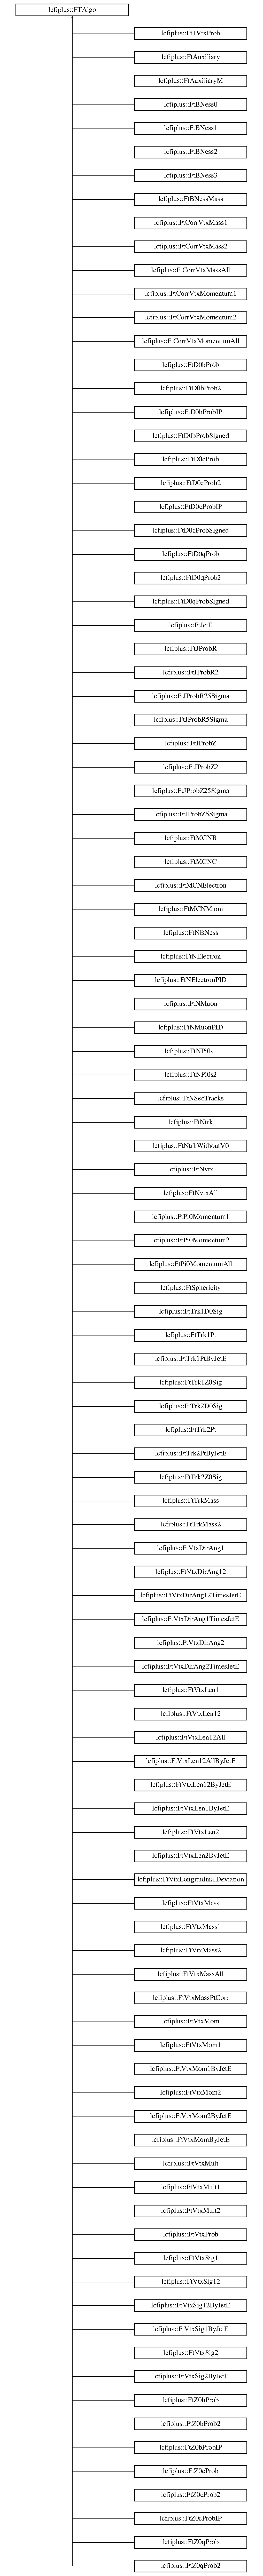
\includegraphics[height=12.000000cm]{classlcfiplus_1_1FTAlgo}
\end{center}
\end{figure}
\subsection*{Public Member Functions}
\begin{DoxyCompactItemize}
\item 
\textbf{ F\+T\+Algo} (string name)
\item 
virtual \textbf{ $\sim$\+F\+T\+Algo} ()
\item 
void \textbf{ set\+Event} (const \textbf{ Event} $\ast$event, const \textbf{ Vertex} $\ast$privtx)
\item 
void \textbf{ set\+Jet} (const \textbf{ Jet} $\ast$jet)
\item 
void \textbf{ set\+N\+Hits\+Joint\+Prob\+D0} (int value)
\item 
void \textbf{ set\+N\+Hits\+Joint\+Prob\+Z0} (int value)
\item 
void \textbf{ set\+N\+Hits\+Most\+Significant\+Track} (int value)
\item 
float \textbf{ get\+Value} ()
\item 
const string \& \textbf{ get\+Name} () const
\item 
float $\ast$ \textbf{ get\+Value\+Address} ()
\item 
virtual void \textbf{ process\+Event} ()
\item 
virtual void \textbf{ process} ()
\end{DoxyCompactItemize}
\subsection*{Protected Attributes}
\begin{DoxyCompactItemize}
\item 
const \textbf{ Event} $\ast$ \textbf{ \+\_\+event}
\item 
const \textbf{ Vertex} $\ast$ \textbf{ \+\_\+privtx}
\item 
const \textbf{ Jet} $\ast$ \textbf{ \+\_\+jet}
\item 
int \textbf{ \+\_\+nhits\+Joint\+Prob\+D0}
\item 
int \textbf{ \+\_\+nhits\+Joint\+Prob\+Z0}
\item 
int \textbf{ \+\_\+nhits\+Most\+Significant\+Track}
\item 
float \textbf{ \+\_\+result}
\item 
string \textbf{ \+\_\+name}
\end{DoxyCompactItemize}


\subsection{Constructor \& Destructor Documentation}
\mbox{\label{classlcfiplus_1_1FTAlgo_a18309a8c94ce19e288f03d48cfe00e79}} 
\index{lcfiplus\+::\+F\+T\+Algo@{lcfiplus\+::\+F\+T\+Algo}!F\+T\+Algo@{F\+T\+Algo}}
\index{F\+T\+Algo@{F\+T\+Algo}!lcfiplus\+::\+F\+T\+Algo@{lcfiplus\+::\+F\+T\+Algo}}
\subsubsection{F\+T\+Algo()}
{\footnotesize\ttfamily lcfiplus\+::\+F\+T\+Algo\+::\+F\+T\+Algo (\begin{DoxyParamCaption}\item[{string}]{name }\end{DoxyParamCaption})\hspace{0.3cm}{\ttfamily [inline]}}

\mbox{\label{classlcfiplus_1_1FTAlgo_af267a08fa8ee5359a53dcd8758828dbd}} 
\index{lcfiplus\+::\+F\+T\+Algo@{lcfiplus\+::\+F\+T\+Algo}!````~F\+T\+Algo@{$\sim$\+F\+T\+Algo}}
\index{````~F\+T\+Algo@{$\sim$\+F\+T\+Algo}!lcfiplus\+::\+F\+T\+Algo@{lcfiplus\+::\+F\+T\+Algo}}
\subsubsection{$\sim$\+F\+T\+Algo()}
{\footnotesize\ttfamily virtual lcfiplus\+::\+F\+T\+Algo\+::$\sim$\+F\+T\+Algo (\begin{DoxyParamCaption}{ }\end{DoxyParamCaption})\hspace{0.3cm}{\ttfamily [inline]}, {\ttfamily [virtual]}}



\subsection{Member Function Documentation}
\mbox{\label{classlcfiplus_1_1FTAlgo_ac76e9ae13546c85c71e2be71542781b0}} 
\index{lcfiplus\+::\+F\+T\+Algo@{lcfiplus\+::\+F\+T\+Algo}!get\+Name@{get\+Name}}
\index{get\+Name@{get\+Name}!lcfiplus\+::\+F\+T\+Algo@{lcfiplus\+::\+F\+T\+Algo}}
\subsubsection{get\+Name()}
{\footnotesize\ttfamily const string\& lcfiplus\+::\+F\+T\+Algo\+::get\+Name (\begin{DoxyParamCaption}{ }\end{DoxyParamCaption}) const\hspace{0.3cm}{\ttfamily [inline]}}



References \+\_\+name.



Referenced by lcfiplus\+::\+F\+T\+Manager\+::get\+Var\+Address(), lcfiplus\+::\+F\+T\+Manager\+::open\+File(), lcfiplus\+::\+F\+T\+Manager\+::open\+Tree(), and lcfiplus\+::\+F\+T\+Manager\+::process().

\mbox{\label{classlcfiplus_1_1FTAlgo_acee17e9515c3ca59b50eae41490c29de}} 
\index{lcfiplus\+::\+F\+T\+Algo@{lcfiplus\+::\+F\+T\+Algo}!get\+Value@{get\+Value}}
\index{get\+Value@{get\+Value}!lcfiplus\+::\+F\+T\+Algo@{lcfiplus\+::\+F\+T\+Algo}}
\subsubsection{get\+Value()}
{\footnotesize\ttfamily float lcfiplus\+::\+F\+T\+Algo\+::get\+Value (\begin{DoxyParamCaption}{ }\end{DoxyParamCaption})}



References \+\_\+result.

\mbox{\label{classlcfiplus_1_1FTAlgo_a61f8d2c2afe4f4d563c43cb0817047e0}} 
\index{lcfiplus\+::\+F\+T\+Algo@{lcfiplus\+::\+F\+T\+Algo}!get\+Value\+Address@{get\+Value\+Address}}
\index{get\+Value\+Address@{get\+Value\+Address}!lcfiplus\+::\+F\+T\+Algo@{lcfiplus\+::\+F\+T\+Algo}}
\subsubsection{get\+Value\+Address()}
{\footnotesize\ttfamily float$\ast$ lcfiplus\+::\+F\+T\+Algo\+::get\+Value\+Address (\begin{DoxyParamCaption}{ }\end{DoxyParamCaption})\hspace{0.3cm}{\ttfamily [inline]}}



References \+\_\+result.



Referenced by lcfiplus\+::\+F\+T\+Manager\+::get\+Var\+Address(), lcfiplus\+::\+F\+T\+Manager\+::open\+File(), and lcfiplus\+::\+F\+T\+Manager\+::open\+Tree().

\mbox{\label{classlcfiplus_1_1FTAlgo_a23cc3f3cd1c100ab6b5e16056112351a}} 
\index{lcfiplus\+::\+F\+T\+Algo@{lcfiplus\+::\+F\+T\+Algo}!process@{process}}
\index{process@{process}!lcfiplus\+::\+F\+T\+Algo@{lcfiplus\+::\+F\+T\+Algo}}
\subsubsection{process()}
{\footnotesize\ttfamily virtual void lcfiplus\+::\+F\+T\+Algo\+::process (\begin{DoxyParamCaption}{ }\end{DoxyParamCaption})\hspace{0.3cm}{\ttfamily [inline]}, {\ttfamily [virtual]}}



Reimplemented in \textbf{ lcfiplus\+::\+Ft\+N\+B\+Ness} \doxyref{}{p.}{classlcfiplus_1_1FtNBNess_af9a1114a1d0f001a10036490570e5a82}, \textbf{ lcfiplus\+::\+Ft\+B\+Ness\+Mass} \doxyref{}{p.}{classlcfiplus_1_1FtBNessMass_aa542017c9cce9c344b674aae68f3084e}, \textbf{ lcfiplus\+::\+Ft\+B\+Ness3} \doxyref{}{p.}{classlcfiplus_1_1FtBNess3_aea7ab74de348d9897b3804d12bd4f938}, \textbf{ lcfiplus\+::\+Ft\+B\+Ness2} \doxyref{}{p.}{classlcfiplus_1_1FtBNess2_a777253ce5623451441076e1f82db65d7}, \textbf{ lcfiplus\+::\+Ft\+B\+Ness1} \doxyref{}{p.}{classlcfiplus_1_1FtBNess1_a91ff1353e4e18811aece7512160fd116}, \textbf{ lcfiplus\+::\+Ft\+B\+Ness0} \doxyref{}{p.}{classlcfiplus_1_1FtBNess0_af8d04b8f7e900520ee4057ad9d27b40f}, \textbf{ lcfiplus\+::\+Ft\+N\+Pi0s2} \doxyref{}{p.}{classlcfiplus_1_1FtNPi0s2_a924b3a544cab8451465c7d33e7480b87}, \textbf{ lcfiplus\+::\+Ft\+N\+Pi0s1} \doxyref{}{p.}{classlcfiplus_1_1FtNPi0s1_a7fdafff17efcbeabf1697488b99cbeae}, \textbf{ lcfiplus\+::\+Ft\+Pi0\+Momentum\+All} \doxyref{}{p.}{classlcfiplus_1_1FtPi0MomentumAll_aac1d58ec21b23c22524859dd71c950c1}, \textbf{ lcfiplus\+::\+Ft\+Pi0\+Momentum2} \doxyref{}{p.}{classlcfiplus_1_1FtPi0Momentum2_aa676b1d5afd4581dabf344232dca8bb9}, \textbf{ lcfiplus\+::\+Ft\+Pi0\+Momentum1} \doxyref{}{p.}{classlcfiplus_1_1FtPi0Momentum1_a28c14c5071b349004b59be4e389713e0}, \textbf{ lcfiplus\+::\+Ft\+Corr\+Vtx\+Momentum\+All} \doxyref{}{p.}{classlcfiplus_1_1FtCorrVtxMomentumAll_a541350ba8ec892f2d86b3072d2b5e3ad}, \textbf{ lcfiplus\+::\+Ft\+Corr\+Vtx\+Momentum2} \doxyref{}{p.}{classlcfiplus_1_1FtCorrVtxMomentum2_a3bbf00a47a5598287aedffbcd7f1f4e7}, \textbf{ lcfiplus\+::\+Ft\+Corr\+Vtx\+Momentum1} \doxyref{}{p.}{classlcfiplus_1_1FtCorrVtxMomentum1_aed6efc62695091f145b3ee80d8d0bbc0}, \textbf{ lcfiplus\+::\+Ft\+Corr\+Vtx\+Mass\+All} \doxyref{}{p.}{classlcfiplus_1_1FtCorrVtxMassAll_a2a48b21fd4d03f7c35bbe71040cec7c9}, \textbf{ lcfiplus\+::\+Ft\+Corr\+Vtx\+Mass2} \doxyref{}{p.}{classlcfiplus_1_1FtCorrVtxMass2_a469cb633f5323240b29ce0779a36f1f7}, \textbf{ lcfiplus\+::\+Ft\+Corr\+Vtx\+Mass1} \doxyref{}{p.}{classlcfiplus_1_1FtCorrVtxMass1_a9854c75f70d16dd4b24ef7e70a4b92dd}, \textbf{ lcfiplus\+::\+Ft\+Z0c\+Prob\+IP} \doxyref{}{p.}{classlcfiplus_1_1FtZ0cProbIP_a26be7b91972ec6e2c165d767c9aedb25}, \textbf{ lcfiplus\+::\+Ft\+Z0b\+Prob\+IP} \doxyref{}{p.}{classlcfiplus_1_1FtZ0bProbIP_a1fff3afba2dcf596886292756283e8c7}, \textbf{ lcfiplus\+::\+Ft\+Z0q\+Prob2} \doxyref{}{p.}{classlcfiplus_1_1FtZ0qProb2_a83ea4dca7b99a30bae246fcf71394246}, \textbf{ lcfiplus\+::\+Ft\+Z0q\+Prob} \doxyref{}{p.}{classlcfiplus_1_1FtZ0qProb_a352fb1ffb695a18a3feef62ffe8cfb74}, \textbf{ lcfiplus\+::\+Ft\+Z0c\+Prob2} \doxyref{}{p.}{classlcfiplus_1_1FtZ0cProb2_af7577bcba793b2204a72885f90b9b830}, \textbf{ lcfiplus\+::\+Ft\+Z0c\+Prob} \doxyref{}{p.}{classlcfiplus_1_1FtZ0cProb_a6421a336a5e0e8cd22f7308350144957}, \textbf{ lcfiplus\+::\+Ft\+Z0b\+Prob2} \doxyref{}{p.}{classlcfiplus_1_1FtZ0bProb2_a105402e137a7c17f0d4ee04505129c7d}, \textbf{ lcfiplus\+::\+Ft\+Z0b\+Prob} \doxyref{}{p.}{classlcfiplus_1_1FtZ0bProb_a6d27f53bc71ed168c1406d52967ee1c2}, \textbf{ lcfiplus\+::\+Ft\+D0c\+Prob\+IP} \doxyref{}{p.}{classlcfiplus_1_1FtD0cProbIP_afb0b4e7c2480d972480aae6860b0ce5a}, \textbf{ lcfiplus\+::\+Ft\+D0b\+Prob\+IP} \doxyref{}{p.}{classlcfiplus_1_1FtD0bProbIP_a8e332673a741c1134d4cb3093be77bde}, \textbf{ lcfiplus\+::\+Ft\+D0q\+Prob\+Signed} \doxyref{}{p.}{classlcfiplus_1_1FtD0qProbSigned_a14df76a1cc006604864aca8617e2b9d2}, \textbf{ lcfiplus\+::\+Ft\+D0c\+Prob\+Signed} \doxyref{}{p.}{classlcfiplus_1_1FtD0cProbSigned_af4849ec51c395a8954ef23374a3d6e48}, \textbf{ lcfiplus\+::\+Ft\+D0b\+Prob\+Signed} \doxyref{}{p.}{classlcfiplus_1_1FtD0bProbSigned_a575e55603f4df3743b3e2a4847355b85}, \textbf{ lcfiplus\+::\+Ft\+D0q\+Prob2} \doxyref{}{p.}{classlcfiplus_1_1FtD0qProb2_aa393b69dfbc040f70cdae5d6edda7a1c}, \textbf{ lcfiplus\+::\+Ft\+D0q\+Prob} \doxyref{}{p.}{classlcfiplus_1_1FtD0qProb_a9f292cfd608518ac59b94a419f3a1f54}, \textbf{ lcfiplus\+::\+Ft\+D0c\+Prob2} \doxyref{}{p.}{classlcfiplus_1_1FtD0cProb2_aba032ecbae4dad88b1e1c75925134046}, \textbf{ lcfiplus\+::\+Ft\+D0c\+Prob} \doxyref{}{p.}{classlcfiplus_1_1FtD0cProb_a3b88af3360cc9ab954541bc5e4554673}, \textbf{ lcfiplus\+::\+Ft\+D0b\+Prob2} \doxyref{}{p.}{classlcfiplus_1_1FtD0bProb2_a2b66e3cd5cfab4dfecdfbb7d76867ad7}, \textbf{ lcfiplus\+::\+Ft\+D0b\+Prob} \doxyref{}{p.}{classlcfiplus_1_1FtD0bProb_aa33fb90a1cb5fc5c444ea9a3317994b9}, \textbf{ lcfiplus\+::\+Ft\+M\+C\+NC} \doxyref{}{p.}{classlcfiplus_1_1FtMCNC_a8832b03425cdc9fc1713c209587d3a20}, \textbf{ lcfiplus\+::\+Ft\+M\+C\+NB} \doxyref{}{p.}{classlcfiplus_1_1FtMCNB_a8495a07421105a91a8fc8f437e7f7e41}, \textbf{ lcfiplus\+::\+Ft\+M\+C\+N\+Electron} \doxyref{}{p.}{classlcfiplus_1_1FtMCNElectron_aa6883f0b241486acdae416e06f5c8d14}, \textbf{ lcfiplus\+::\+Ft\+M\+C\+N\+Muon} \doxyref{}{p.}{classlcfiplus_1_1FtMCNMuon_a257089c0418ddb5bad6d4f644462b98c}, \textbf{ lcfiplus\+::\+Ft\+N\+Muon\+P\+ID} \doxyref{}{p.}{classlcfiplus_1_1FtNMuonPID_aa11ced9d3f89b6046206df1fb3ef879e}, \textbf{ lcfiplus\+::\+Ft\+N\+Electron\+P\+ID} \doxyref{}{p.}{classlcfiplus_1_1FtNElectronPID_a6b4cb272635b48c13c3acd2810cab715}, \textbf{ lcfiplus\+::\+Ft\+N\+Electron} \doxyref{}{p.}{classlcfiplus_1_1FtNElectron_a2beafefb58d803a1af565c11f301eab8}, \textbf{ lcfiplus\+::\+Ft\+N\+Muon} \doxyref{}{p.}{classlcfiplus_1_1FtNMuon_adc2c58022919b1732aa130148e4ee068}, \textbf{ lcfiplus\+::\+Ft\+Vtx\+Longitudinal\+Deviation} \doxyref{}{p.}{classlcfiplus_1_1FtVtxLongitudinalDeviation_a09c2c20c11802a7dcd85f21e9a3b0cb3}, \textbf{ lcfiplus\+::\+Ft\+N\+Sec\+Tracks} \doxyref{}{p.}{classlcfiplus_1_1FtNSecTracks_aa83884b0ee9505e92f2051b1a925569a}, \textbf{ lcfiplus\+::\+Ft\+Trk\+Mass2} \doxyref{}{p.}{classlcfiplus_1_1FtTrkMass2_a12798546edfab6fc39ada5ed3aa28c12}, \textbf{ lcfiplus\+::\+Ft\+Trk\+Mass} \doxyref{}{p.}{classlcfiplus_1_1FtTrkMass_ad4e922e5aff8b6129f1d9dd6d45da461}, \textbf{ lcfiplus\+::\+Ft\+Sphericity} \doxyref{}{p.}{classlcfiplus_1_1FtSphericity_aae492dec997d4e4ed2774e41f5429a7d}, \textbf{ lcfiplus\+::\+Ft\+J\+Prob\+Z25\+Sigma} \doxyref{}{p.}{classlcfiplus_1_1FtJProbZ25Sigma_a166ae515e6a478e74877d5ed2db243bf}, \textbf{ lcfiplus\+::\+Ft\+J\+Prob\+R25\+Sigma} \doxyref{}{p.}{classlcfiplus_1_1FtJProbR25Sigma_a4023aebf51a661e640842bf6006facaa}, \textbf{ lcfiplus\+::\+Ft\+J\+Prob\+Z2} \doxyref{}{p.}{classlcfiplus_1_1FtJProbZ2_a8fcb9cd0ca85e631f6ebba7dd8681f0c}, \textbf{ lcfiplus\+::\+Ft\+J\+Prob\+R2} \doxyref{}{p.}{classlcfiplus_1_1FtJProbR2_abdc160e02a597230ffead6a04147e9f4}, \textbf{ lcfiplus\+::\+Ft\+J\+Prob\+Z5\+Sigma} \doxyref{}{p.}{classlcfiplus_1_1FtJProbZ5Sigma_acabdb6a10a791978f4fdf5c77111726d}, \textbf{ lcfiplus\+::\+Ft\+J\+Prob\+R5\+Sigma} \doxyref{}{p.}{classlcfiplus_1_1FtJProbR5Sigma_aeaf2eec741c8f11a7534eac003401007}, \textbf{ lcfiplus\+::\+Ft\+J\+ProbZ} \doxyref{}{p.}{classlcfiplus_1_1FtJProbZ_aeae617aa635e1ec77a4ab1235448ac35}, \textbf{ lcfiplus\+::\+Ft\+J\+ProbR} \doxyref{}{p.}{classlcfiplus_1_1FtJProbR_a8bca5390b49033530ceec071aca60762}, \textbf{ lcfiplus\+::\+Ft\+Trk2\+Pt\+By\+JetE} \doxyref{}{p.}{classlcfiplus_1_1FtTrk2PtByJetE_a2bf84efcb9445254559dd792f05142cd}, \textbf{ lcfiplus\+::\+Ft\+Trk1\+Pt\+By\+JetE} \doxyref{}{p.}{classlcfiplus_1_1FtTrk1PtByJetE_a62bffce7f7aa2f04955af9942d83778f}, \textbf{ lcfiplus\+::\+Ft\+Trk2\+Pt} \doxyref{}{p.}{classlcfiplus_1_1FtTrk2Pt_a71ee427b434dca028bc460b112271654}, \textbf{ lcfiplus\+::\+Ft\+Trk1\+Pt} \doxyref{}{p.}{classlcfiplus_1_1FtTrk1Pt_abcc889e774fe3bf5a1cf7be55f235bcc}, \textbf{ lcfiplus\+::\+Ft\+Trk2\+Z0\+Sig} \doxyref{}{p.}{classlcfiplus_1_1FtTrk2Z0Sig_ab08166ac62a893ebf5ecc2282b889ecb}, \textbf{ lcfiplus\+::\+Ft\+Trk1\+Z0\+Sig} \doxyref{}{p.}{classlcfiplus_1_1FtTrk1Z0Sig_a254b45dc2e1f2fa4f1f2ff7313f2e2db}, \textbf{ lcfiplus\+::\+Ft\+Trk2\+D0\+Sig} \doxyref{}{p.}{classlcfiplus_1_1FtTrk2D0Sig_ae8f2ba348322a8bffb379480a8bbeb93}, \textbf{ lcfiplus\+::\+Ft\+Trk1\+D0\+Sig} \doxyref{}{p.}{classlcfiplus_1_1FtTrk1D0Sig_a60d4f8688341c6ed7e156d55f47071fb}, \textbf{ lcfiplus\+::\+Ft\+Vtx\+Mult2} \doxyref{}{p.}{classlcfiplus_1_1FtVtxMult2_aeba9c8e3dbd47de0d8ab41918e7efefc}, \textbf{ lcfiplus\+::\+Ft\+Vtx\+Mult1} \doxyref{}{p.}{classlcfiplus_1_1FtVtxMult1_af9ec09d21643b55ded80b11991eea801}, \textbf{ lcfiplus\+::\+Ft\+Vtx\+Mult} \doxyref{}{p.}{classlcfiplus_1_1FtVtxMult_a9f7f885a9cc05627574231f7080effdd}, \textbf{ lcfiplus\+::\+Ft\+Vtx\+Mass2} \doxyref{}{p.}{classlcfiplus_1_1FtVtxMass2_a5a608c80cff2827515f3023c5fbd875e}, \textbf{ lcfiplus\+::\+Ft\+Vtx\+Mass1} \doxyref{}{p.}{classlcfiplus_1_1FtVtxMass1_a39edfa0bc88f4aa2302466c0f5fa3e42}, \textbf{ lcfiplus\+::\+Ft\+Vtx\+Mass} \doxyref{}{p.}{classlcfiplus_1_1FtVtxMass_a68f7a29e7781b612b55626160db226cc}, \textbf{ lcfiplus\+::\+Ft\+Vtx\+Prob} \doxyref{}{p.}{classlcfiplus_1_1FtVtxProb_af2aea188e06463875859a06e758346f8}, \textbf{ lcfiplus\+::\+Ft\+Vtx\+Mass\+Pt\+Corr} \doxyref{}{p.}{classlcfiplus_1_1FtVtxMassPtCorr_a4548a4904e91d0046b22c2a0ee91ed23}, \textbf{ lcfiplus\+::\+Ft\+Vtx\+Mom2\+By\+JetE} \doxyref{}{p.}{classlcfiplus_1_1FtVtxMom2ByJetE_a029a38e007d9905dfad972deb1facf03}, \textbf{ lcfiplus\+::\+Ft\+Vtx\+Mom1\+By\+JetE} \doxyref{}{p.}{classlcfiplus_1_1FtVtxMom1ByJetE_a5383c444edf2a1cf3f0a57250c79ac5d}, \textbf{ lcfiplus\+::\+Ft\+Vtx\+Mom\+By\+JetE} \doxyref{}{p.}{classlcfiplus_1_1FtVtxMomByJetE_af84866a2fe7170465b0379082db94380}, \textbf{ lcfiplus\+::\+Ft\+Vtx\+Mom2} \doxyref{}{p.}{classlcfiplus_1_1FtVtxMom2_a2c8b056bdee18283fb7aebc07cdc3904}, \textbf{ lcfiplus\+::\+Ft\+Vtx\+Mom1} \doxyref{}{p.}{classlcfiplus_1_1FtVtxMom1_a220f239f33e36a724e1c2ea52b474269}, \textbf{ lcfiplus\+::\+Ft\+Vtx\+Mom} \doxyref{}{p.}{classlcfiplus_1_1FtVtxMom_a5084c2c18c43b29f14db6cb208e2fbca}, \textbf{ lcfiplus\+::\+Ft\+Vtx\+Dir\+Ang12\+Times\+JetE} \doxyref{}{p.}{classlcfiplus_1_1FtVtxDirAng12TimesJetE_a47c27ed04146b14a35a20f60d31ac0d5}, \textbf{ lcfiplus\+::\+Ft\+Vtx\+Dir\+Ang2\+Times\+JetE} \doxyref{}{p.}{classlcfiplus_1_1FtVtxDirAng2TimesJetE_a347f269fe151dd63ba3a87521edf1337}, \textbf{ lcfiplus\+::\+Ft\+Vtx\+Dir\+Ang1\+Times\+JetE} \doxyref{}{p.}{classlcfiplus_1_1FtVtxDirAng1TimesJetE_a89477c43c615630152abcbddd4e125be}, \textbf{ lcfiplus\+::\+Ft\+Vtx\+Dir\+Ang12} \doxyref{}{p.}{classlcfiplus_1_1FtVtxDirAng12_a28ff3b7778f404dd1ea9a09c3a7a554c}, \textbf{ lcfiplus\+::\+Ft\+Vtx\+Dir\+Ang2} \doxyref{}{p.}{classlcfiplus_1_1FtVtxDirAng2_a1083a33352880b11c7bc341e286c5111}, \textbf{ lcfiplus\+::\+Ft\+Vtx\+Dir\+Ang1} \doxyref{}{p.}{classlcfiplus_1_1FtVtxDirAng1_ae741908744bbc9a859b313033d836d57}, \textbf{ lcfiplus\+::\+Ft\+Vtx\+Sig12\+By\+JetE} \doxyref{}{p.}{classlcfiplus_1_1FtVtxSig12ByJetE_a4c444fe1243d24a58f2b2257ac6b82fa}, \textbf{ lcfiplus\+::\+Ft\+Vtx\+Sig2\+By\+JetE} \doxyref{}{p.}{classlcfiplus_1_1FtVtxSig2ByJetE_aed16e786431b1e0b16dfc563080f165b}, \textbf{ lcfiplus\+::\+Ft\+Vtx\+Sig1\+By\+JetE} \doxyref{}{p.}{classlcfiplus_1_1FtVtxSig1ByJetE_abb86953e2039954d74568a2cb041a219}, \textbf{ lcfiplus\+::\+Ft\+Vtx\+Sig12} \doxyref{}{p.}{classlcfiplus_1_1FtVtxSig12_ab30a72fd89f34f96a33082d95dad5630}, \textbf{ lcfiplus\+::\+Ft\+Vtx\+Sig2} \doxyref{}{p.}{classlcfiplus_1_1FtVtxSig2_ad9ee270ed49ec11808c259b2aaea80c3}, \textbf{ lcfiplus\+::\+Ft\+Vtx\+Sig1} \doxyref{}{p.}{classlcfiplus_1_1FtVtxSig1_a6aae4d789f6e3e402a25a529b689e4f6}, \textbf{ lcfiplus\+::\+Ft\+Vtx\+Len12\+By\+JetE} \doxyref{}{p.}{classlcfiplus_1_1FtVtxLen12ByJetE_aca8743034a4ef3aef41757abd1c5e89e}, \textbf{ lcfiplus\+::\+Ft\+Vtx\+Len2\+By\+JetE} \doxyref{}{p.}{classlcfiplus_1_1FtVtxLen2ByJetE_a27517a6ebfedb5f7a8ad31452519fe09}, \textbf{ lcfiplus\+::\+Ft\+Vtx\+Len1\+By\+JetE} \doxyref{}{p.}{classlcfiplus_1_1FtVtxLen1ByJetE_a35dc0c77214951f224b1bb79e5fc17ca}, \textbf{ lcfiplus\+::\+Ft\+Vtx\+Len12} \doxyref{}{p.}{classlcfiplus_1_1FtVtxLen12_a795a6c5f1f2b210bee84cbd966a7ee6c}, \textbf{ lcfiplus\+::\+Ft\+Vtx\+Len2} \doxyref{}{p.}{classlcfiplus_1_1FtVtxLen2_a137f42d4ef11154f1fb95b4063a1e334}, \textbf{ lcfiplus\+::\+Ft\+Vtx\+Len1} \doxyref{}{p.}{classlcfiplus_1_1FtVtxLen1_a1e12d61253c3771de132b8d43f0ff123}, \textbf{ lcfiplus\+::\+Ft\+JetE} \doxyref{}{p.}{classlcfiplus_1_1FtJetE_ab39abe153f0a14a4aa5de8145d6d1e30}, \textbf{ lcfiplus\+::\+Ft\+Nvtx} \doxyref{}{p.}{classlcfiplus_1_1FtNvtx_af1d407d62e17ea231e299838c7795f46}, \textbf{ lcfiplus\+::\+Ft1\+Vtx\+Prob} \doxyref{}{p.}{classlcfiplus_1_1Ft1VtxProb_ad74ede9d41a8727cd2aae354d1690743}, \textbf{ lcfiplus\+::\+Ft\+Vtx\+Len12\+All\+By\+JetE} \doxyref{}{p.}{classlcfiplus_1_1FtVtxLen12AllByJetE_a7be7b6a99d26c08a3894cc2fab6acfa9}, \textbf{ lcfiplus\+::\+Ft\+Vtx\+Len12\+All} \doxyref{}{p.}{classlcfiplus_1_1FtVtxLen12All_ae67541407b33577ff49f5be788692c27}, \textbf{ lcfiplus\+::\+Ft\+Vtx\+Mass\+All} \doxyref{}{p.}{classlcfiplus_1_1FtVtxMassAll_a32942f93b2008c86797d123b8932113c}, \textbf{ lcfiplus\+::\+Ft\+Nvtx\+All} \doxyref{}{p.}{classlcfiplus_1_1FtNvtxAll_afdad8e549b571380cca394cab1cb24ca}, \textbf{ lcfiplus\+::\+Ft\+Ntrk} \doxyref{}{p.}{classlcfiplus_1_1FtNtrk_a4f85046fdadbb3d63fa3e16d73e4927b}, \textbf{ lcfiplus\+::\+Ft\+Ntrk\+Without\+V0} \doxyref{}{p.}{classlcfiplus_1_1FtNtrkWithoutV0_a1c17b675542cd448e3e720525c14e6dd}, \textbf{ lcfiplus\+::\+Ft\+AuxiliaryM} \doxyref{}{p.}{classlcfiplus_1_1FtAuxiliaryM_a2c0df248a7f26d0cdcaa7483f9829e0a}, and \textbf{ lcfiplus\+::\+Ft\+Auxiliary} \doxyref{}{p.}{classlcfiplus_1_1FtAuxiliary_aafb10984a9f3e5d054ea7601ea23477c}.



Referenced by lcfiplus\+::\+F\+T\+Manager\+::process().

\mbox{\label{classlcfiplus_1_1FTAlgo_a4b22a0cc29f4dc2045ba2770ab30a128}} 
\index{lcfiplus\+::\+F\+T\+Algo@{lcfiplus\+::\+F\+T\+Algo}!process\+Event@{process\+Event}}
\index{process\+Event@{process\+Event}!lcfiplus\+::\+F\+T\+Algo@{lcfiplus\+::\+F\+T\+Algo}}
\subsubsection{process\+Event()}
{\footnotesize\ttfamily virtual void lcfiplus\+::\+F\+T\+Algo\+::process\+Event (\begin{DoxyParamCaption}{ }\end{DoxyParamCaption})\hspace{0.3cm}{\ttfamily [inline]}, {\ttfamily [virtual]}}



Reimplemented in \textbf{ lcfiplus\+::\+Ft\+M\+C\+NC} \doxyref{}{p.}{classlcfiplus_1_1FtMCNC_af577b1bad0f22f3ad28db551534a455a}, and \textbf{ lcfiplus\+::\+Ft\+M\+C\+NB} \doxyref{}{p.}{classlcfiplus_1_1FtMCNB_a98f262af3450b8f201bb1ae24dcf5a93}.



Referenced by lcfiplus\+::\+F\+T\+Manager\+::process().

\mbox{\label{classlcfiplus_1_1FTAlgo_ac49764d7d0e38c42b7094d90568788ec}} 
\index{lcfiplus\+::\+F\+T\+Algo@{lcfiplus\+::\+F\+T\+Algo}!set\+Event@{set\+Event}}
\index{set\+Event@{set\+Event}!lcfiplus\+::\+F\+T\+Algo@{lcfiplus\+::\+F\+T\+Algo}}
\subsubsection{set\+Event()}
{\footnotesize\ttfamily void lcfiplus\+::\+F\+T\+Algo\+::set\+Event (\begin{DoxyParamCaption}\item[{const \textbf{ Event} $\ast$}]{event,  }\item[{const \textbf{ Vertex} $\ast$}]{privtx }\end{DoxyParamCaption})}



References \+\_\+event, and \+\_\+privtx.



Referenced by lcfiplus\+::\+F\+T\+Manager\+::process().

\mbox{\label{classlcfiplus_1_1FTAlgo_a5692d90a2bacb05037f50343c0c963d7}} 
\index{lcfiplus\+::\+F\+T\+Algo@{lcfiplus\+::\+F\+T\+Algo}!set\+Jet@{set\+Jet}}
\index{set\+Jet@{set\+Jet}!lcfiplus\+::\+F\+T\+Algo@{lcfiplus\+::\+F\+T\+Algo}}
\subsubsection{set\+Jet()}
{\footnotesize\ttfamily void lcfiplus\+::\+F\+T\+Algo\+::set\+Jet (\begin{DoxyParamCaption}\item[{const \textbf{ Jet} $\ast$}]{jet }\end{DoxyParamCaption})}



References \+\_\+jet.



Referenced by lcfiplus\+::\+F\+T\+Manager\+::process().

\mbox{\label{classlcfiplus_1_1FTAlgo_adb5db810a0a2ae3f947bfadc01c0ddf0}} 
\index{lcfiplus\+::\+F\+T\+Algo@{lcfiplus\+::\+F\+T\+Algo}!set\+N\+Hits\+Joint\+Prob\+D0@{set\+N\+Hits\+Joint\+Prob\+D0}}
\index{set\+N\+Hits\+Joint\+Prob\+D0@{set\+N\+Hits\+Joint\+Prob\+D0}!lcfiplus\+::\+F\+T\+Algo@{lcfiplus\+::\+F\+T\+Algo}}
\subsubsection{set\+N\+Hits\+Joint\+Prob\+D0()}
{\footnotesize\ttfamily void lcfiplus\+::\+F\+T\+Algo\+::set\+N\+Hits\+Joint\+Prob\+D0 (\begin{DoxyParamCaption}\item[{int}]{value }\end{DoxyParamCaption})}



References \+\_\+nhits\+Joint\+Prob\+D0.



Referenced by lcfiplus\+::\+F\+T\+Manager\+::process().

\mbox{\label{classlcfiplus_1_1FTAlgo_a5c7e3e599a4089265c4fe4f9a9aa08f6}} 
\index{lcfiplus\+::\+F\+T\+Algo@{lcfiplus\+::\+F\+T\+Algo}!set\+N\+Hits\+Joint\+Prob\+Z0@{set\+N\+Hits\+Joint\+Prob\+Z0}}
\index{set\+N\+Hits\+Joint\+Prob\+Z0@{set\+N\+Hits\+Joint\+Prob\+Z0}!lcfiplus\+::\+F\+T\+Algo@{lcfiplus\+::\+F\+T\+Algo}}
\subsubsection{set\+N\+Hits\+Joint\+Prob\+Z0()}
{\footnotesize\ttfamily void lcfiplus\+::\+F\+T\+Algo\+::set\+N\+Hits\+Joint\+Prob\+Z0 (\begin{DoxyParamCaption}\item[{int}]{value }\end{DoxyParamCaption})}



References \+\_\+nhits\+Joint\+Prob\+Z0.



Referenced by lcfiplus\+::\+F\+T\+Manager\+::process().

\mbox{\label{classlcfiplus_1_1FTAlgo_ae64a5269b5dc42b68b249873cac33ebc}} 
\index{lcfiplus\+::\+F\+T\+Algo@{lcfiplus\+::\+F\+T\+Algo}!set\+N\+Hits\+Most\+Significant\+Track@{set\+N\+Hits\+Most\+Significant\+Track}}
\index{set\+N\+Hits\+Most\+Significant\+Track@{set\+N\+Hits\+Most\+Significant\+Track}!lcfiplus\+::\+F\+T\+Algo@{lcfiplus\+::\+F\+T\+Algo}}
\subsubsection{set\+N\+Hits\+Most\+Significant\+Track()}
{\footnotesize\ttfamily void lcfiplus\+::\+F\+T\+Algo\+::set\+N\+Hits\+Most\+Significant\+Track (\begin{DoxyParamCaption}\item[{int}]{value }\end{DoxyParamCaption})}



References \+\_\+nhits\+Most\+Significant\+Track.



Referenced by lcfiplus\+::\+F\+T\+Manager\+::process().



\subsection{Member Data Documentation}
\mbox{\label{classlcfiplus_1_1FTAlgo_a3509085db2dcd973ab4471a6bd9204c8}} 
\index{lcfiplus\+::\+F\+T\+Algo@{lcfiplus\+::\+F\+T\+Algo}!\+\_\+event@{\+\_\+event}}
\index{\+\_\+event@{\+\_\+event}!lcfiplus\+::\+F\+T\+Algo@{lcfiplus\+::\+F\+T\+Algo}}
\subsubsection{\+\_\+event}
{\footnotesize\ttfamily const \textbf{ Event}$\ast$ lcfiplus\+::\+F\+T\+Algo\+::\+\_\+event\hspace{0.3cm}{\ttfamily [protected]}}



Referenced by set\+Event().

\mbox{\label{classlcfiplus_1_1FTAlgo_a3d335341927f3f889d7edee065f1f5c9}} 
\index{lcfiplus\+::\+F\+T\+Algo@{lcfiplus\+::\+F\+T\+Algo}!\+\_\+jet@{\+\_\+jet}}
\index{\+\_\+jet@{\+\_\+jet}!lcfiplus\+::\+F\+T\+Algo@{lcfiplus\+::\+F\+T\+Algo}}
\subsubsection{\+\_\+jet}
{\footnotesize\ttfamily const \textbf{ Jet}$\ast$ lcfiplus\+::\+F\+T\+Algo\+::\+\_\+jet\hspace{0.3cm}{\ttfamily [protected]}}



Referenced by set\+Jet().

\mbox{\label{classlcfiplus_1_1FTAlgo_aa23a75f0f0bf4af0760609eefec0dd3c}} 
\index{lcfiplus\+::\+F\+T\+Algo@{lcfiplus\+::\+F\+T\+Algo}!\+\_\+name@{\+\_\+name}}
\index{\+\_\+name@{\+\_\+name}!lcfiplus\+::\+F\+T\+Algo@{lcfiplus\+::\+F\+T\+Algo}}
\subsubsection{\+\_\+name}
{\footnotesize\ttfamily string lcfiplus\+::\+F\+T\+Algo\+::\+\_\+name\hspace{0.3cm}{\ttfamily [protected]}}



Referenced by get\+Name().

\mbox{\label{classlcfiplus_1_1FTAlgo_afd447cf5dd7b88a3b4b6a88525c0df98}} 
\index{lcfiplus\+::\+F\+T\+Algo@{lcfiplus\+::\+F\+T\+Algo}!\+\_\+nhits\+Joint\+Prob\+D0@{\+\_\+nhits\+Joint\+Prob\+D0}}
\index{\+\_\+nhits\+Joint\+Prob\+D0@{\+\_\+nhits\+Joint\+Prob\+D0}!lcfiplus\+::\+F\+T\+Algo@{lcfiplus\+::\+F\+T\+Algo}}
\subsubsection{\+\_\+nhits\+Joint\+Prob\+D0}
{\footnotesize\ttfamily int lcfiplus\+::\+F\+T\+Algo\+::\+\_\+nhits\+Joint\+Prob\+D0\hspace{0.3cm}{\ttfamily [protected]}}



Referenced by set\+N\+Hits\+Joint\+Prob\+D0().

\mbox{\label{classlcfiplus_1_1FTAlgo_af9e2f019041855d28895ee89a318891e}} 
\index{lcfiplus\+::\+F\+T\+Algo@{lcfiplus\+::\+F\+T\+Algo}!\+\_\+nhits\+Joint\+Prob\+Z0@{\+\_\+nhits\+Joint\+Prob\+Z0}}
\index{\+\_\+nhits\+Joint\+Prob\+Z0@{\+\_\+nhits\+Joint\+Prob\+Z0}!lcfiplus\+::\+F\+T\+Algo@{lcfiplus\+::\+F\+T\+Algo}}
\subsubsection{\+\_\+nhits\+Joint\+Prob\+Z0}
{\footnotesize\ttfamily int lcfiplus\+::\+F\+T\+Algo\+::\+\_\+nhits\+Joint\+Prob\+Z0\hspace{0.3cm}{\ttfamily [protected]}}



Referenced by set\+N\+Hits\+Joint\+Prob\+Z0().

\mbox{\label{classlcfiplus_1_1FTAlgo_aecf97b44577f63419e77a98f92a64c3c}} 
\index{lcfiplus\+::\+F\+T\+Algo@{lcfiplus\+::\+F\+T\+Algo}!\+\_\+nhits\+Most\+Significant\+Track@{\+\_\+nhits\+Most\+Significant\+Track}}
\index{\+\_\+nhits\+Most\+Significant\+Track@{\+\_\+nhits\+Most\+Significant\+Track}!lcfiplus\+::\+F\+T\+Algo@{lcfiplus\+::\+F\+T\+Algo}}
\subsubsection{\+\_\+nhits\+Most\+Significant\+Track}
{\footnotesize\ttfamily int lcfiplus\+::\+F\+T\+Algo\+::\+\_\+nhits\+Most\+Significant\+Track\hspace{0.3cm}{\ttfamily [protected]}}



Referenced by set\+N\+Hits\+Most\+Significant\+Track().

\mbox{\label{classlcfiplus_1_1FTAlgo_aa9fb98a9e80c976f6fa231048dbf4645}} 
\index{lcfiplus\+::\+F\+T\+Algo@{lcfiplus\+::\+F\+T\+Algo}!\+\_\+privtx@{\+\_\+privtx}}
\index{\+\_\+privtx@{\+\_\+privtx}!lcfiplus\+::\+F\+T\+Algo@{lcfiplus\+::\+F\+T\+Algo}}
\subsubsection{\+\_\+privtx}
{\footnotesize\ttfamily const \textbf{ Vertex}$\ast$ lcfiplus\+::\+F\+T\+Algo\+::\+\_\+privtx\hspace{0.3cm}{\ttfamily [protected]}}



Referenced by set\+Event().

\mbox{\label{classlcfiplus_1_1FTAlgo_a1237a9bafb00e4e85d11e8171158d567}} 
\index{lcfiplus\+::\+F\+T\+Algo@{lcfiplus\+::\+F\+T\+Algo}!\+\_\+result@{\+\_\+result}}
\index{\+\_\+result@{\+\_\+result}!lcfiplus\+::\+F\+T\+Algo@{lcfiplus\+::\+F\+T\+Algo}}
\subsubsection{\+\_\+result}
{\footnotesize\ttfamily float lcfiplus\+::\+F\+T\+Algo\+::\+\_\+result\hspace{0.3cm}{\ttfamily [protected]}}



Referenced by get\+Value(), and get\+Value\+Address().



The documentation for this class was generated from the following files\+:\begin{DoxyCompactItemize}
\item 
\textbf{ flavtag.\+h}\item 
\textbf{ flavtag.\+cc}\end{DoxyCompactItemize}

\section{lcfiplus\+:\+:Ft\+Auxiliary Class Reference}
\label{classlcfiplus_1_1FtAuxiliary}\index{lcfiplus\+::\+Ft\+Auxiliary@{lcfiplus\+::\+Ft\+Auxiliary}}
Inheritance diagram for lcfiplus\+:\+:Ft\+Auxiliary\+:\begin{figure}[H]
\begin{center}
\leavevmode
\includegraphics[height=2.000000cm]{classlcfiplus_1_1FtAuxiliary}
\end{center}
\end{figure}
\subsection*{Public Member Functions}
\begin{DoxyCompactItemize}
\item 
\textbf{ Ft\+Auxiliary} (const char $\ast$auxname, int auxval)
\item 
void \textbf{ process} ()
\end{DoxyCompactItemize}
\subsection*{Additional Inherited Members}


\subsection{Constructor \& Destructor Documentation}
\mbox{\label{classlcfiplus_1_1FtAuxiliary_ad29ce89189c60cf5b80043cc21e2aebf}} 
\index{lcfiplus\+::\+Ft\+Auxiliary@{lcfiplus\+::\+Ft\+Auxiliary}!Ft\+Auxiliary@{Ft\+Auxiliary}}
\index{Ft\+Auxiliary@{Ft\+Auxiliary}!lcfiplus\+::\+Ft\+Auxiliary@{lcfiplus\+::\+Ft\+Auxiliary}}
\subsubsection{Ft\+Auxiliary()}
{\footnotesize\ttfamily lcfiplus\+::\+Ft\+Auxiliary\+::\+Ft\+Auxiliary (\begin{DoxyParamCaption}\item[{const char $\ast$}]{auxname,  }\item[{int}]{auxval }\end{DoxyParamCaption})\hspace{0.3cm}{\ttfamily [inline]}}



\subsection{Member Function Documentation}
\mbox{\label{classlcfiplus_1_1FtAuxiliary_aafb10984a9f3e5d054ea7601ea23477c}} 
\index{lcfiplus\+::\+Ft\+Auxiliary@{lcfiplus\+::\+Ft\+Auxiliary}!process@{process}}
\index{process@{process}!lcfiplus\+::\+Ft\+Auxiliary@{lcfiplus\+::\+Ft\+Auxiliary}}
\subsubsection{process()}
{\footnotesize\ttfamily void lcfiplus\+::\+Ft\+Auxiliary\+::process (\begin{DoxyParamCaption}{ }\end{DoxyParamCaption})\hspace{0.3cm}{\ttfamily [inline]}, {\ttfamily [virtual]}}



Reimplemented from \textbf{ lcfiplus\+::\+F\+T\+Algo} \doxyref{}{p.}{classlcfiplus_1_1FTAlgo_a23cc3f3cd1c100ab6b5e16056112351a}.



The documentation for this class was generated from the following file\+:\begin{DoxyCompactItemize}
\item 
\textbf{ Flavor\+Tag.\+cc}\end{DoxyCompactItemize}

\section{lcfiplus\+:\+:Ft\+AuxiliaryM Class Reference}
\label{classlcfiplus_1_1FtAuxiliaryM}\index{lcfiplus\+::\+Ft\+AuxiliaryM@{lcfiplus\+::\+Ft\+AuxiliaryM}}
Inheritance diagram for lcfiplus\+:\+:Ft\+AuxiliaryM\+:\begin{figure}[H]
\begin{center}
\leavevmode
\includegraphics[height=2.000000cm]{classlcfiplus_1_1FtAuxiliaryM}
\end{center}
\end{figure}
\subsection*{Public Member Functions}
\begin{DoxyCompactItemize}
\item 
\textbf{ Ft\+AuxiliaryM} (const char $\ast$auxname)
\item 
void \textbf{ process} ()
\end{DoxyCompactItemize}
\subsection*{Additional Inherited Members}


\subsection{Constructor \& Destructor Documentation}
\mbox{\label{classlcfiplus_1_1FtAuxiliaryM_a478e4c75189b35a7a03c3af89b683a55}} 
\index{lcfiplus\+::\+Ft\+AuxiliaryM@{lcfiplus\+::\+Ft\+AuxiliaryM}!Ft\+AuxiliaryM@{Ft\+AuxiliaryM}}
\index{Ft\+AuxiliaryM@{Ft\+AuxiliaryM}!lcfiplus\+::\+Ft\+AuxiliaryM@{lcfiplus\+::\+Ft\+AuxiliaryM}}
\subsubsection{Ft\+Auxiliary\+M()}
{\footnotesize\ttfamily lcfiplus\+::\+Ft\+Auxiliary\+M\+::\+Ft\+AuxiliaryM (\begin{DoxyParamCaption}\item[{const char $\ast$}]{auxname }\end{DoxyParamCaption})\hspace{0.3cm}{\ttfamily [inline]}}



\subsection{Member Function Documentation}
\mbox{\label{classlcfiplus_1_1FtAuxiliaryM_a2c0df248a7f26d0cdcaa7483f9829e0a}} 
\index{lcfiplus\+::\+Ft\+AuxiliaryM@{lcfiplus\+::\+Ft\+AuxiliaryM}!process@{process}}
\index{process@{process}!lcfiplus\+::\+Ft\+AuxiliaryM@{lcfiplus\+::\+Ft\+AuxiliaryM}}
\subsubsection{process()}
{\footnotesize\ttfamily void lcfiplus\+::\+Ft\+Auxiliary\+M\+::process (\begin{DoxyParamCaption}{ }\end{DoxyParamCaption})\hspace{0.3cm}{\ttfamily [inline]}, {\ttfamily [virtual]}}



Reimplemented from \textbf{ lcfiplus\+::\+F\+T\+Algo} \doxyref{}{p.}{classlcfiplus_1_1FTAlgo_a23cc3f3cd1c100ab6b5e16056112351a}.



References lcfiplus\+::\+F\+T\+Manager\+::get\+Auxiliary(), and lcfiplus\+::\+F\+T\+Manager\+::get\+Instance().



The documentation for this class was generated from the following file\+:\begin{DoxyCompactItemize}
\item 
\textbf{ Flavor\+Tag.\+cc}\end{DoxyCompactItemize}

\section{lcfiplus\+:\+:Ft\+B\+Ness0 Class Reference}
\label{classlcfiplus_1_1FtBNess0}\index{lcfiplus\+::\+Ft\+B\+Ness0@{lcfiplus\+::\+Ft\+B\+Ness0}}
Inheritance diagram for lcfiplus\+:\+:Ft\+B\+Ness0\+:\begin{figure}[H]
\begin{center}
\leavevmode
\includegraphics[height=2.000000cm]{classlcfiplus_1_1FtBNess0}
\end{center}
\end{figure}
\subsection*{Public Member Functions}
\begin{DoxyCompactItemize}
\item 
\textbf{ Ft\+B\+Ness0} ()
\item 
void \textbf{ process} ()
\end{DoxyCompactItemize}
\subsection*{Additional Inherited Members}


\subsection{Constructor \& Destructor Documentation}
\mbox{\label{classlcfiplus_1_1FtBNess0_acfac6ca9baa0ba428f902fd972bff8cc}} 
\index{lcfiplus\+::\+Ft\+B\+Ness0@{lcfiplus\+::\+Ft\+B\+Ness0}!Ft\+B\+Ness0@{Ft\+B\+Ness0}}
\index{Ft\+B\+Ness0@{Ft\+B\+Ness0}!lcfiplus\+::\+Ft\+B\+Ness0@{lcfiplus\+::\+Ft\+B\+Ness0}}
\subsubsection{Ft\+B\+Ness0()}
{\footnotesize\ttfamily lcfiplus\+::\+Ft\+B\+Ness0\+::\+Ft\+B\+Ness0 (\begin{DoxyParamCaption}{ }\end{DoxyParamCaption})\hspace{0.3cm}{\ttfamily [inline]}}



\subsection{Member Function Documentation}
\mbox{\label{classlcfiplus_1_1FtBNess0_af8d04b8f7e900520ee4057ad9d27b40f}} 
\index{lcfiplus\+::\+Ft\+B\+Ness0@{lcfiplus\+::\+Ft\+B\+Ness0}!process@{process}}
\index{process@{process}!lcfiplus\+::\+Ft\+B\+Ness0@{lcfiplus\+::\+Ft\+B\+Ness0}}
\subsubsection{process()}
{\footnotesize\ttfamily void lcfiplus\+::\+Ft\+B\+Ness0\+::process (\begin{DoxyParamCaption}{ }\end{DoxyParamCaption})\hspace{0.3cm}{\ttfamily [inline]}, {\ttfamily [virtual]}}



Reimplemented from \textbf{ lcfiplus\+::\+F\+T\+Algo} \doxyref{}{p.}{classlcfiplus_1_1FTAlgo_a23cc3f3cd1c100ab6b5e16056112351a}.



The documentation for this class was generated from the following file\+:\begin{DoxyCompactItemize}
\item 
\textbf{ Flavor\+Tag.\+cc}\end{DoxyCompactItemize}

\section{lcfiplus\+:\+:Ft\+B\+Ness1 Class Reference}
\label{classlcfiplus_1_1FtBNess1}\index{lcfiplus\+::\+Ft\+B\+Ness1@{lcfiplus\+::\+Ft\+B\+Ness1}}
Inheritance diagram for lcfiplus\+:\+:Ft\+B\+Ness1\+:\begin{figure}[H]
\begin{center}
\leavevmode
\includegraphics[height=2.000000cm]{classlcfiplus_1_1FtBNess1}
\end{center}
\end{figure}
\subsection*{Public Member Functions}
\begin{DoxyCompactItemize}
\item 
\textbf{ Ft\+B\+Ness1} ()
\item 
void \textbf{ process} ()
\end{DoxyCompactItemize}
\subsection*{Additional Inherited Members}


\subsection{Constructor \& Destructor Documentation}
\mbox{\label{classlcfiplus_1_1FtBNess1_a1919be68bbbe084621c6d387536a3cb2}} 
\index{lcfiplus\+::\+Ft\+B\+Ness1@{lcfiplus\+::\+Ft\+B\+Ness1}!Ft\+B\+Ness1@{Ft\+B\+Ness1}}
\index{Ft\+B\+Ness1@{Ft\+B\+Ness1}!lcfiplus\+::\+Ft\+B\+Ness1@{lcfiplus\+::\+Ft\+B\+Ness1}}
\subsubsection{Ft\+B\+Ness1()}
{\footnotesize\ttfamily lcfiplus\+::\+Ft\+B\+Ness1\+::\+Ft\+B\+Ness1 (\begin{DoxyParamCaption}{ }\end{DoxyParamCaption})\hspace{0.3cm}{\ttfamily [inline]}}



\subsection{Member Function Documentation}
\mbox{\label{classlcfiplus_1_1FtBNess1_a91ff1353e4e18811aece7512160fd116}} 
\index{lcfiplus\+::\+Ft\+B\+Ness1@{lcfiplus\+::\+Ft\+B\+Ness1}!process@{process}}
\index{process@{process}!lcfiplus\+::\+Ft\+B\+Ness1@{lcfiplus\+::\+Ft\+B\+Ness1}}
\subsubsection{process()}
{\footnotesize\ttfamily void lcfiplus\+::\+Ft\+B\+Ness1\+::process (\begin{DoxyParamCaption}{ }\end{DoxyParamCaption})\hspace{0.3cm}{\ttfamily [inline]}, {\ttfamily [virtual]}}



Reimplemented from \textbf{ lcfiplus\+::\+F\+T\+Algo} \doxyref{}{p.}{classlcfiplus_1_1FTAlgo_a23cc3f3cd1c100ab6b5e16056112351a}.



The documentation for this class was generated from the following file\+:\begin{DoxyCompactItemize}
\item 
\textbf{ Flavor\+Tag.\+cc}\end{DoxyCompactItemize}

\section{lcfiplus\+:\+:Ft\+B\+Ness2 Class Reference}
\label{classlcfiplus_1_1FtBNess2}\index{lcfiplus\+::\+Ft\+B\+Ness2@{lcfiplus\+::\+Ft\+B\+Ness2}}
Inheritance diagram for lcfiplus\+:\+:Ft\+B\+Ness2\+:\begin{figure}[H]
\begin{center}
\leavevmode
\includegraphics[height=2.000000cm]{classlcfiplus_1_1FtBNess2}
\end{center}
\end{figure}
\subsection*{Public Member Functions}
\begin{DoxyCompactItemize}
\item 
\textbf{ Ft\+B\+Ness2} ()
\item 
void \textbf{ process} ()
\end{DoxyCompactItemize}
\subsection*{Additional Inherited Members}


\subsection{Constructor \& Destructor Documentation}
\mbox{\label{classlcfiplus_1_1FtBNess2_a865234c66df797b918a0564e19aad423}} 
\index{lcfiplus\+::\+Ft\+B\+Ness2@{lcfiplus\+::\+Ft\+B\+Ness2}!Ft\+B\+Ness2@{Ft\+B\+Ness2}}
\index{Ft\+B\+Ness2@{Ft\+B\+Ness2}!lcfiplus\+::\+Ft\+B\+Ness2@{lcfiplus\+::\+Ft\+B\+Ness2}}
\subsubsection{Ft\+B\+Ness2()}
{\footnotesize\ttfamily lcfiplus\+::\+Ft\+B\+Ness2\+::\+Ft\+B\+Ness2 (\begin{DoxyParamCaption}{ }\end{DoxyParamCaption})\hspace{0.3cm}{\ttfamily [inline]}}



\subsection{Member Function Documentation}
\mbox{\label{classlcfiplus_1_1FtBNess2_a777253ce5623451441076e1f82db65d7}} 
\index{lcfiplus\+::\+Ft\+B\+Ness2@{lcfiplus\+::\+Ft\+B\+Ness2}!process@{process}}
\index{process@{process}!lcfiplus\+::\+Ft\+B\+Ness2@{lcfiplus\+::\+Ft\+B\+Ness2}}
\subsubsection{process()}
{\footnotesize\ttfamily void lcfiplus\+::\+Ft\+B\+Ness2\+::process (\begin{DoxyParamCaption}{ }\end{DoxyParamCaption})\hspace{0.3cm}{\ttfamily [inline]}, {\ttfamily [virtual]}}



Reimplemented from \textbf{ lcfiplus\+::\+F\+T\+Algo} \doxyref{}{p.}{classlcfiplus_1_1FTAlgo_a23cc3f3cd1c100ab6b5e16056112351a}.



The documentation for this class was generated from the following file\+:\begin{DoxyCompactItemize}
\item 
\textbf{ Flavor\+Tag.\+cc}\end{DoxyCompactItemize}

\section{lcfiplus\+:\+:Ft\+B\+Ness3 Class Reference}
\label{classlcfiplus_1_1FtBNess3}\index{lcfiplus\+::\+Ft\+B\+Ness3@{lcfiplus\+::\+Ft\+B\+Ness3}}
Inheritance diagram for lcfiplus\+:\+:Ft\+B\+Ness3\+:\begin{figure}[H]
\begin{center}
\leavevmode
\includegraphics[height=2.000000cm]{classlcfiplus_1_1FtBNess3}
\end{center}
\end{figure}
\subsection*{Public Member Functions}
\begin{DoxyCompactItemize}
\item 
\textbf{ Ft\+B\+Ness3} ()
\item 
void \textbf{ process} ()
\end{DoxyCompactItemize}
\subsection*{Additional Inherited Members}


\subsection{Constructor \& Destructor Documentation}
\mbox{\label{classlcfiplus_1_1FtBNess3_aa74a35db7857c356b6b24e1d4a504ae9}} 
\index{lcfiplus\+::\+Ft\+B\+Ness3@{lcfiplus\+::\+Ft\+B\+Ness3}!Ft\+B\+Ness3@{Ft\+B\+Ness3}}
\index{Ft\+B\+Ness3@{Ft\+B\+Ness3}!lcfiplus\+::\+Ft\+B\+Ness3@{lcfiplus\+::\+Ft\+B\+Ness3}}
\subsubsection{Ft\+B\+Ness3()}
{\footnotesize\ttfamily lcfiplus\+::\+Ft\+B\+Ness3\+::\+Ft\+B\+Ness3 (\begin{DoxyParamCaption}{ }\end{DoxyParamCaption})\hspace{0.3cm}{\ttfamily [inline]}}



\subsection{Member Function Documentation}
\mbox{\label{classlcfiplus_1_1FtBNess3_aea7ab74de348d9897b3804d12bd4f938}} 
\index{lcfiplus\+::\+Ft\+B\+Ness3@{lcfiplus\+::\+Ft\+B\+Ness3}!process@{process}}
\index{process@{process}!lcfiplus\+::\+Ft\+B\+Ness3@{lcfiplus\+::\+Ft\+B\+Ness3}}
\subsubsection{process()}
{\footnotesize\ttfamily void lcfiplus\+::\+Ft\+B\+Ness3\+::process (\begin{DoxyParamCaption}{ }\end{DoxyParamCaption})\hspace{0.3cm}{\ttfamily [inline]}, {\ttfamily [virtual]}}



Reimplemented from \textbf{ lcfiplus\+::\+F\+T\+Algo} \doxyref{}{p.}{classlcfiplus_1_1FTAlgo_a23cc3f3cd1c100ab6b5e16056112351a}.



The documentation for this class was generated from the following file\+:\begin{DoxyCompactItemize}
\item 
\textbf{ Flavor\+Tag.\+cc}\end{DoxyCompactItemize}

\section{lcfiplus\+:\+:Ft\+B\+Ness\+Mass Class Reference}
\label{classlcfiplus_1_1FtBNessMass}\index{lcfiplus\+::\+Ft\+B\+Ness\+Mass@{lcfiplus\+::\+Ft\+B\+Ness\+Mass}}
Inheritance diagram for lcfiplus\+:\+:Ft\+B\+Ness\+Mass\+:\begin{figure}[H]
\begin{center}
\leavevmode
\includegraphics[height=2.000000cm]{classlcfiplus_1_1FtBNessMass}
\end{center}
\end{figure}
\subsection*{Public Member Functions}
\begin{DoxyCompactItemize}
\item 
\textbf{ Ft\+B\+Ness\+Mass} ()
\item 
void \textbf{ process} ()
\end{DoxyCompactItemize}
\subsection*{Additional Inherited Members}


\subsection{Constructor \& Destructor Documentation}
\mbox{\label{classlcfiplus_1_1FtBNessMass_a4fde092e92a3b8e7e5572643ea1196f6}} 
\index{lcfiplus\+::\+Ft\+B\+Ness\+Mass@{lcfiplus\+::\+Ft\+B\+Ness\+Mass}!Ft\+B\+Ness\+Mass@{Ft\+B\+Ness\+Mass}}
\index{Ft\+B\+Ness\+Mass@{Ft\+B\+Ness\+Mass}!lcfiplus\+::\+Ft\+B\+Ness\+Mass@{lcfiplus\+::\+Ft\+B\+Ness\+Mass}}
\subsubsection{Ft\+B\+Ness\+Mass()}
{\footnotesize\ttfamily lcfiplus\+::\+Ft\+B\+Ness\+Mass\+::\+Ft\+B\+Ness\+Mass (\begin{DoxyParamCaption}{ }\end{DoxyParamCaption})\hspace{0.3cm}{\ttfamily [inline]}}



\subsection{Member Function Documentation}
\mbox{\label{classlcfiplus_1_1FtBNessMass_aa542017c9cce9c344b674aae68f3084e}} 
\index{lcfiplus\+::\+Ft\+B\+Ness\+Mass@{lcfiplus\+::\+Ft\+B\+Ness\+Mass}!process@{process}}
\index{process@{process}!lcfiplus\+::\+Ft\+B\+Ness\+Mass@{lcfiplus\+::\+Ft\+B\+Ness\+Mass}}
\subsubsection{process()}
{\footnotesize\ttfamily void lcfiplus\+::\+Ft\+B\+Ness\+Mass\+::process (\begin{DoxyParamCaption}{ }\end{DoxyParamCaption})\hspace{0.3cm}{\ttfamily [inline]}, {\ttfamily [virtual]}}



Reimplemented from \textbf{ lcfiplus\+::\+F\+T\+Algo} \doxyref{}{p.}{classlcfiplus_1_1FTAlgo_a23cc3f3cd1c100ab6b5e16056112351a}.



The documentation for this class was generated from the following file\+:\begin{DoxyCompactItemize}
\item 
\textbf{ Flavor\+Tag.\+cc}\end{DoxyCompactItemize}

\section{lcfiplus\+:\+:Ft\+Corr\+Vtx\+Mass1 Class Reference}
\label{classlcfiplus_1_1FtCorrVtxMass1}\index{lcfiplus\+::\+Ft\+Corr\+Vtx\+Mass1@{lcfiplus\+::\+Ft\+Corr\+Vtx\+Mass1}}
Inheritance diagram for lcfiplus\+:\+:Ft\+Corr\+Vtx\+Mass1\+:\begin{figure}[H]
\begin{center}
\leavevmode
\includegraphics[height=2.000000cm]{classlcfiplus_1_1FtCorrVtxMass1}
\end{center}
\end{figure}
\subsection*{Public Member Functions}
\begin{DoxyCompactItemize}
\item 
\textbf{ Ft\+Corr\+Vtx\+Mass1} ()
\item 
void \textbf{ process} ()
\end{DoxyCompactItemize}
\subsection*{Additional Inherited Members}


\subsection{Constructor \& Destructor Documentation}
\mbox{\label{classlcfiplus_1_1FtCorrVtxMass1_a108fe06d88d4c2c8b477c52844650a12}} 
\index{lcfiplus\+::\+Ft\+Corr\+Vtx\+Mass1@{lcfiplus\+::\+Ft\+Corr\+Vtx\+Mass1}!Ft\+Corr\+Vtx\+Mass1@{Ft\+Corr\+Vtx\+Mass1}}
\index{Ft\+Corr\+Vtx\+Mass1@{Ft\+Corr\+Vtx\+Mass1}!lcfiplus\+::\+Ft\+Corr\+Vtx\+Mass1@{lcfiplus\+::\+Ft\+Corr\+Vtx\+Mass1}}
\subsubsection{Ft\+Corr\+Vtx\+Mass1()}
{\footnotesize\ttfamily lcfiplus\+::\+Ft\+Corr\+Vtx\+Mass1\+::\+Ft\+Corr\+Vtx\+Mass1 (\begin{DoxyParamCaption}{ }\end{DoxyParamCaption})\hspace{0.3cm}{\ttfamily [inline]}}



\subsection{Member Function Documentation}
\mbox{\label{classlcfiplus_1_1FtCorrVtxMass1_a9854c75f70d16dd4b24ef7e70a4b92dd}} 
\index{lcfiplus\+::\+Ft\+Corr\+Vtx\+Mass1@{lcfiplus\+::\+Ft\+Corr\+Vtx\+Mass1}!process@{process}}
\index{process@{process}!lcfiplus\+::\+Ft\+Corr\+Vtx\+Mass1@{lcfiplus\+::\+Ft\+Corr\+Vtx\+Mass1}}
\subsubsection{process()}
{\footnotesize\ttfamily void lcfiplus\+::\+Ft\+Corr\+Vtx\+Mass1\+::process (\begin{DoxyParamCaption}{ }\end{DoxyParamCaption})\hspace{0.3cm}{\ttfamily [inline]}, {\ttfamily [virtual]}}



Reimplemented from \textbf{ lcfiplus\+::\+F\+T\+Algo} \doxyref{}{p.}{classlcfiplus_1_1FTAlgo_a23cc3f3cd1c100ab6b5e16056112351a}.



The documentation for this class was generated from the following file\+:\begin{DoxyCompactItemize}
\item 
\textbf{ Flavor\+Tag.\+cc}\end{DoxyCompactItemize}

\section{lcfiplus\+:\+:Ft\+Corr\+Vtx\+Mass2 Class Reference}
\label{classlcfiplus_1_1FtCorrVtxMass2}\index{lcfiplus\+::\+Ft\+Corr\+Vtx\+Mass2@{lcfiplus\+::\+Ft\+Corr\+Vtx\+Mass2}}
Inheritance diagram for lcfiplus\+:\+:Ft\+Corr\+Vtx\+Mass2\+:\begin{figure}[H]
\begin{center}
\leavevmode
\includegraphics[height=2.000000cm]{classlcfiplus_1_1FtCorrVtxMass2}
\end{center}
\end{figure}
\subsection*{Public Member Functions}
\begin{DoxyCompactItemize}
\item 
\textbf{ Ft\+Corr\+Vtx\+Mass2} ()
\item 
void \textbf{ process} ()
\end{DoxyCompactItemize}
\subsection*{Additional Inherited Members}


\subsection{Constructor \& Destructor Documentation}
\mbox{\label{classlcfiplus_1_1FtCorrVtxMass2_a11e0a5263d367f8b935411ca4e92fda4}} 
\index{lcfiplus\+::\+Ft\+Corr\+Vtx\+Mass2@{lcfiplus\+::\+Ft\+Corr\+Vtx\+Mass2}!Ft\+Corr\+Vtx\+Mass2@{Ft\+Corr\+Vtx\+Mass2}}
\index{Ft\+Corr\+Vtx\+Mass2@{Ft\+Corr\+Vtx\+Mass2}!lcfiplus\+::\+Ft\+Corr\+Vtx\+Mass2@{lcfiplus\+::\+Ft\+Corr\+Vtx\+Mass2}}
\subsubsection{Ft\+Corr\+Vtx\+Mass2()}
{\footnotesize\ttfamily lcfiplus\+::\+Ft\+Corr\+Vtx\+Mass2\+::\+Ft\+Corr\+Vtx\+Mass2 (\begin{DoxyParamCaption}{ }\end{DoxyParamCaption})\hspace{0.3cm}{\ttfamily [inline]}}



\subsection{Member Function Documentation}
\mbox{\label{classlcfiplus_1_1FtCorrVtxMass2_a469cb633f5323240b29ce0779a36f1f7}} 
\index{lcfiplus\+::\+Ft\+Corr\+Vtx\+Mass2@{lcfiplus\+::\+Ft\+Corr\+Vtx\+Mass2}!process@{process}}
\index{process@{process}!lcfiplus\+::\+Ft\+Corr\+Vtx\+Mass2@{lcfiplus\+::\+Ft\+Corr\+Vtx\+Mass2}}
\subsubsection{process()}
{\footnotesize\ttfamily void lcfiplus\+::\+Ft\+Corr\+Vtx\+Mass2\+::process (\begin{DoxyParamCaption}{ }\end{DoxyParamCaption})\hspace{0.3cm}{\ttfamily [inline]}, {\ttfamily [virtual]}}



Reimplemented from \textbf{ lcfiplus\+::\+F\+T\+Algo} \doxyref{}{p.}{classlcfiplus_1_1FTAlgo_a23cc3f3cd1c100ab6b5e16056112351a}.



The documentation for this class was generated from the following file\+:\begin{DoxyCompactItemize}
\item 
\textbf{ Flavor\+Tag.\+cc}\end{DoxyCompactItemize}

\section{lcfiplus\+:\+:Ft\+Corr\+Vtx\+Mass\+All Class Reference}
\label{classlcfiplus_1_1FtCorrVtxMassAll}\index{lcfiplus\+::\+Ft\+Corr\+Vtx\+Mass\+All@{lcfiplus\+::\+Ft\+Corr\+Vtx\+Mass\+All}}
Inheritance diagram for lcfiplus\+:\+:Ft\+Corr\+Vtx\+Mass\+All\+:\begin{figure}[H]
\begin{center}
\leavevmode
\includegraphics[height=2.000000cm]{classlcfiplus_1_1FtCorrVtxMassAll}
\end{center}
\end{figure}
\subsection*{Public Member Functions}
\begin{DoxyCompactItemize}
\item 
\textbf{ Ft\+Corr\+Vtx\+Mass\+All} ()
\item 
void \textbf{ process} ()
\end{DoxyCompactItemize}
\subsection*{Additional Inherited Members}


\subsection{Constructor \& Destructor Documentation}
\mbox{\label{classlcfiplus_1_1FtCorrVtxMassAll_a2f8cb131ee0dc92148e30ec95c97f7c1}} 
\index{lcfiplus\+::\+Ft\+Corr\+Vtx\+Mass\+All@{lcfiplus\+::\+Ft\+Corr\+Vtx\+Mass\+All}!Ft\+Corr\+Vtx\+Mass\+All@{Ft\+Corr\+Vtx\+Mass\+All}}
\index{Ft\+Corr\+Vtx\+Mass\+All@{Ft\+Corr\+Vtx\+Mass\+All}!lcfiplus\+::\+Ft\+Corr\+Vtx\+Mass\+All@{lcfiplus\+::\+Ft\+Corr\+Vtx\+Mass\+All}}
\subsubsection{Ft\+Corr\+Vtx\+Mass\+All()}
{\footnotesize\ttfamily lcfiplus\+::\+Ft\+Corr\+Vtx\+Mass\+All\+::\+Ft\+Corr\+Vtx\+Mass\+All (\begin{DoxyParamCaption}{ }\end{DoxyParamCaption})\hspace{0.3cm}{\ttfamily [inline]}}



\subsection{Member Function Documentation}
\mbox{\label{classlcfiplus_1_1FtCorrVtxMassAll_a2a48b21fd4d03f7c35bbe71040cec7c9}} 
\index{lcfiplus\+::\+Ft\+Corr\+Vtx\+Mass\+All@{lcfiplus\+::\+Ft\+Corr\+Vtx\+Mass\+All}!process@{process}}
\index{process@{process}!lcfiplus\+::\+Ft\+Corr\+Vtx\+Mass\+All@{lcfiplus\+::\+Ft\+Corr\+Vtx\+Mass\+All}}
\subsubsection{process()}
{\footnotesize\ttfamily void lcfiplus\+::\+Ft\+Corr\+Vtx\+Mass\+All\+::process (\begin{DoxyParamCaption}{ }\end{DoxyParamCaption})\hspace{0.3cm}{\ttfamily [inline]}, {\ttfamily [virtual]}}



Reimplemented from \textbf{ lcfiplus\+::\+F\+T\+Algo} \doxyref{}{p.}{classlcfiplus_1_1FTAlgo_a23cc3f3cd1c100ab6b5e16056112351a}.



The documentation for this class was generated from the following file\+:\begin{DoxyCompactItemize}
\item 
\textbf{ Flavor\+Tag.\+cc}\end{DoxyCompactItemize}

\section{lcfiplus\+:\+:Ft\+Corr\+Vtx\+Momentum1 Class Reference}
\label{classlcfiplus_1_1FtCorrVtxMomentum1}\index{lcfiplus\+::\+Ft\+Corr\+Vtx\+Momentum1@{lcfiplus\+::\+Ft\+Corr\+Vtx\+Momentum1}}
Inheritance diagram for lcfiplus\+:\+:Ft\+Corr\+Vtx\+Momentum1\+:\begin{figure}[H]
\begin{center}
\leavevmode
\includegraphics[height=2.000000cm]{classlcfiplus_1_1FtCorrVtxMomentum1}
\end{center}
\end{figure}
\subsection*{Public Member Functions}
\begin{DoxyCompactItemize}
\item 
\textbf{ Ft\+Corr\+Vtx\+Momentum1} ()
\item 
void \textbf{ process} ()
\end{DoxyCompactItemize}
\subsection*{Additional Inherited Members}


\subsection{Constructor \& Destructor Documentation}
\mbox{\label{classlcfiplus_1_1FtCorrVtxMomentum1_a830d7cce56f862c1b9bad1279956cbe6}} 
\index{lcfiplus\+::\+Ft\+Corr\+Vtx\+Momentum1@{lcfiplus\+::\+Ft\+Corr\+Vtx\+Momentum1}!Ft\+Corr\+Vtx\+Momentum1@{Ft\+Corr\+Vtx\+Momentum1}}
\index{Ft\+Corr\+Vtx\+Momentum1@{Ft\+Corr\+Vtx\+Momentum1}!lcfiplus\+::\+Ft\+Corr\+Vtx\+Momentum1@{lcfiplus\+::\+Ft\+Corr\+Vtx\+Momentum1}}
\subsubsection{Ft\+Corr\+Vtx\+Momentum1()}
{\footnotesize\ttfamily lcfiplus\+::\+Ft\+Corr\+Vtx\+Momentum1\+::\+Ft\+Corr\+Vtx\+Momentum1 (\begin{DoxyParamCaption}{ }\end{DoxyParamCaption})\hspace{0.3cm}{\ttfamily [inline]}}



\subsection{Member Function Documentation}
\mbox{\label{classlcfiplus_1_1FtCorrVtxMomentum1_aed6efc62695091f145b3ee80d8d0bbc0}} 
\index{lcfiplus\+::\+Ft\+Corr\+Vtx\+Momentum1@{lcfiplus\+::\+Ft\+Corr\+Vtx\+Momentum1}!process@{process}}
\index{process@{process}!lcfiplus\+::\+Ft\+Corr\+Vtx\+Momentum1@{lcfiplus\+::\+Ft\+Corr\+Vtx\+Momentum1}}
\subsubsection{process()}
{\footnotesize\ttfamily void lcfiplus\+::\+Ft\+Corr\+Vtx\+Momentum1\+::process (\begin{DoxyParamCaption}{ }\end{DoxyParamCaption})\hspace{0.3cm}{\ttfamily [inline]}, {\ttfamily [virtual]}}



Reimplemented from \textbf{ lcfiplus\+::\+F\+T\+Algo} \doxyref{}{p.}{classlcfiplus_1_1FTAlgo_a23cc3f3cd1c100ab6b5e16056112351a}.



The documentation for this class was generated from the following file\+:\begin{DoxyCompactItemize}
\item 
\textbf{ Flavor\+Tag.\+cc}\end{DoxyCompactItemize}

\section{lcfiplus\+:\+:Ft\+Corr\+Vtx\+Momentum2 Class Reference}
\label{classlcfiplus_1_1FtCorrVtxMomentum2}\index{lcfiplus\+::\+Ft\+Corr\+Vtx\+Momentum2@{lcfiplus\+::\+Ft\+Corr\+Vtx\+Momentum2}}
Inheritance diagram for lcfiplus\+:\+:Ft\+Corr\+Vtx\+Momentum2\+:\begin{figure}[H]
\begin{center}
\leavevmode
\includegraphics[height=2.000000cm]{classlcfiplus_1_1FtCorrVtxMomentum2}
\end{center}
\end{figure}
\subsection*{Public Member Functions}
\begin{DoxyCompactItemize}
\item 
\textbf{ Ft\+Corr\+Vtx\+Momentum2} ()
\item 
void \textbf{ process} ()
\end{DoxyCompactItemize}
\subsection*{Additional Inherited Members}


\subsection{Constructor \& Destructor Documentation}
\mbox{\label{classlcfiplus_1_1FtCorrVtxMomentum2_aa93675795b86a694ecf41a853e503fdd}} 
\index{lcfiplus\+::\+Ft\+Corr\+Vtx\+Momentum2@{lcfiplus\+::\+Ft\+Corr\+Vtx\+Momentum2}!Ft\+Corr\+Vtx\+Momentum2@{Ft\+Corr\+Vtx\+Momentum2}}
\index{Ft\+Corr\+Vtx\+Momentum2@{Ft\+Corr\+Vtx\+Momentum2}!lcfiplus\+::\+Ft\+Corr\+Vtx\+Momentum2@{lcfiplus\+::\+Ft\+Corr\+Vtx\+Momentum2}}
\subsubsection{Ft\+Corr\+Vtx\+Momentum2()}
{\footnotesize\ttfamily lcfiplus\+::\+Ft\+Corr\+Vtx\+Momentum2\+::\+Ft\+Corr\+Vtx\+Momentum2 (\begin{DoxyParamCaption}{ }\end{DoxyParamCaption})\hspace{0.3cm}{\ttfamily [inline]}}



\subsection{Member Function Documentation}
\mbox{\label{classlcfiplus_1_1FtCorrVtxMomentum2_a3bbf00a47a5598287aedffbcd7f1f4e7}} 
\index{lcfiplus\+::\+Ft\+Corr\+Vtx\+Momentum2@{lcfiplus\+::\+Ft\+Corr\+Vtx\+Momentum2}!process@{process}}
\index{process@{process}!lcfiplus\+::\+Ft\+Corr\+Vtx\+Momentum2@{lcfiplus\+::\+Ft\+Corr\+Vtx\+Momentum2}}
\subsubsection{process()}
{\footnotesize\ttfamily void lcfiplus\+::\+Ft\+Corr\+Vtx\+Momentum2\+::process (\begin{DoxyParamCaption}{ }\end{DoxyParamCaption})\hspace{0.3cm}{\ttfamily [inline]}, {\ttfamily [virtual]}}



Reimplemented from \textbf{ lcfiplus\+::\+F\+T\+Algo} \doxyref{}{p.}{classlcfiplus_1_1FTAlgo_a23cc3f3cd1c100ab6b5e16056112351a}.



The documentation for this class was generated from the following file\+:\begin{DoxyCompactItemize}
\item 
\textbf{ Flavor\+Tag.\+cc}\end{DoxyCompactItemize}

\section{lcfiplus\+:\+:Ft\+Corr\+Vtx\+Momentum\+All Class Reference}
\label{classlcfiplus_1_1FtCorrVtxMomentumAll}\index{lcfiplus\+::\+Ft\+Corr\+Vtx\+Momentum\+All@{lcfiplus\+::\+Ft\+Corr\+Vtx\+Momentum\+All}}
Inheritance diagram for lcfiplus\+:\+:Ft\+Corr\+Vtx\+Momentum\+All\+:\begin{figure}[H]
\begin{center}
\leavevmode
\includegraphics[height=2.000000cm]{classlcfiplus_1_1FtCorrVtxMomentumAll}
\end{center}
\end{figure}
\subsection*{Public Member Functions}
\begin{DoxyCompactItemize}
\item 
\textbf{ Ft\+Corr\+Vtx\+Momentum\+All} ()
\item 
void \textbf{ process} ()
\end{DoxyCompactItemize}
\subsection*{Additional Inherited Members}


\subsection{Constructor \& Destructor Documentation}
\mbox{\label{classlcfiplus_1_1FtCorrVtxMomentumAll_a1f8959948b3bd1066ca325e598e9c06d}} 
\index{lcfiplus\+::\+Ft\+Corr\+Vtx\+Momentum\+All@{lcfiplus\+::\+Ft\+Corr\+Vtx\+Momentum\+All}!Ft\+Corr\+Vtx\+Momentum\+All@{Ft\+Corr\+Vtx\+Momentum\+All}}
\index{Ft\+Corr\+Vtx\+Momentum\+All@{Ft\+Corr\+Vtx\+Momentum\+All}!lcfiplus\+::\+Ft\+Corr\+Vtx\+Momentum\+All@{lcfiplus\+::\+Ft\+Corr\+Vtx\+Momentum\+All}}
\subsubsection{Ft\+Corr\+Vtx\+Momentum\+All()}
{\footnotesize\ttfamily lcfiplus\+::\+Ft\+Corr\+Vtx\+Momentum\+All\+::\+Ft\+Corr\+Vtx\+Momentum\+All (\begin{DoxyParamCaption}{ }\end{DoxyParamCaption})\hspace{0.3cm}{\ttfamily [inline]}}



\subsection{Member Function Documentation}
\mbox{\label{classlcfiplus_1_1FtCorrVtxMomentumAll_a541350ba8ec892f2d86b3072d2b5e3ad}} 
\index{lcfiplus\+::\+Ft\+Corr\+Vtx\+Momentum\+All@{lcfiplus\+::\+Ft\+Corr\+Vtx\+Momentum\+All}!process@{process}}
\index{process@{process}!lcfiplus\+::\+Ft\+Corr\+Vtx\+Momentum\+All@{lcfiplus\+::\+Ft\+Corr\+Vtx\+Momentum\+All}}
\subsubsection{process()}
{\footnotesize\ttfamily void lcfiplus\+::\+Ft\+Corr\+Vtx\+Momentum\+All\+::process (\begin{DoxyParamCaption}{ }\end{DoxyParamCaption})\hspace{0.3cm}{\ttfamily [inline]}, {\ttfamily [virtual]}}



Reimplemented from \textbf{ lcfiplus\+::\+F\+T\+Algo} \doxyref{}{p.}{classlcfiplus_1_1FTAlgo_a23cc3f3cd1c100ab6b5e16056112351a}.



The documentation for this class was generated from the following file\+:\begin{DoxyCompactItemize}
\item 
\textbf{ Flavor\+Tag.\+cc}\end{DoxyCompactItemize}

\section{lcfiplus\+:\+:Ft\+D0b\+Prob Class Reference}
\label{classlcfiplus_1_1FtD0bProb}\index{lcfiplus\+::\+Ft\+D0b\+Prob@{lcfiplus\+::\+Ft\+D0b\+Prob}}
Inheritance diagram for lcfiplus\+:\+:Ft\+D0b\+Prob\+:\begin{figure}[H]
\begin{center}
\leavevmode
\includegraphics[height=2.000000cm]{classlcfiplus_1_1FtD0bProb}
\end{center}
\end{figure}
\subsection*{Public Member Functions}
\begin{DoxyCompactItemize}
\item 
\textbf{ Ft\+D0b\+Prob} ()
\item 
void \textbf{ process} ()
\end{DoxyCompactItemize}
\subsection*{Additional Inherited Members}


\subsection{Constructor \& Destructor Documentation}
\mbox{\label{classlcfiplus_1_1FtD0bProb_a186f503c80290b84878e12b14732c502}} 
\index{lcfiplus\+::\+Ft\+D0b\+Prob@{lcfiplus\+::\+Ft\+D0b\+Prob}!Ft\+D0b\+Prob@{Ft\+D0b\+Prob}}
\index{Ft\+D0b\+Prob@{Ft\+D0b\+Prob}!lcfiplus\+::\+Ft\+D0b\+Prob@{lcfiplus\+::\+Ft\+D0b\+Prob}}
\subsubsection{Ft\+D0b\+Prob()}
{\footnotesize\ttfamily lcfiplus\+::\+Ft\+D0b\+Prob\+::\+Ft\+D0b\+Prob (\begin{DoxyParamCaption}{ }\end{DoxyParamCaption})\hspace{0.3cm}{\ttfamily [inline]}}



\subsection{Member Function Documentation}
\mbox{\label{classlcfiplus_1_1FtD0bProb_aa33fb90a1cb5fc5c444ea9a3317994b9}} 
\index{lcfiplus\+::\+Ft\+D0b\+Prob@{lcfiplus\+::\+Ft\+D0b\+Prob}!process@{process}}
\index{process@{process}!lcfiplus\+::\+Ft\+D0b\+Prob@{lcfiplus\+::\+Ft\+D0b\+Prob}}
\subsubsection{process()}
{\footnotesize\ttfamily void lcfiplus\+::\+Ft\+D0b\+Prob\+::process (\begin{DoxyParamCaption}{ }\end{DoxyParamCaption})\hspace{0.3cm}{\ttfamily [inline]}, {\ttfamily [virtual]}}



Reimplemented from \textbf{ lcfiplus\+::\+F\+T\+Algo} \doxyref{}{p.}{classlcfiplus_1_1FTAlgo_a23cc3f3cd1c100ab6b5e16056112351a}.



References lcfiplus\+::\+F\+T\+Manager\+::get\+Instance(), lcfiplus\+::\+F\+T\+Manager\+::get\+I\+P\+Prob\+Holder(), and lcfiplus\+::algo\+Sig\+Prob\+::track\+D0\+Significance().



The documentation for this class was generated from the following file\+:\begin{DoxyCompactItemize}
\item 
\textbf{ Flavor\+Tag.\+cc}\end{DoxyCompactItemize}

\section{lcfiplus\+:\+:Ft\+D0b\+Prob2 Class Reference}
\label{classlcfiplus_1_1FtD0bProb2}\index{lcfiplus\+::\+Ft\+D0b\+Prob2@{lcfiplus\+::\+Ft\+D0b\+Prob2}}
Inheritance diagram for lcfiplus\+:\+:Ft\+D0b\+Prob2\+:\begin{figure}[H]
\begin{center}
\leavevmode
\includegraphics[height=2.000000cm]{classlcfiplus_1_1FtD0bProb2}
\end{center}
\end{figure}
\subsection*{Public Member Functions}
\begin{DoxyCompactItemize}
\item 
\textbf{ Ft\+D0b\+Prob2} ()
\item 
void \textbf{ process} ()
\end{DoxyCompactItemize}
\subsection*{Additional Inherited Members}


\subsection{Constructor \& Destructor Documentation}
\mbox{\label{classlcfiplus_1_1FtD0bProb2_a6d60b2dacff72b42e7d5df175633f3cf}} 
\index{lcfiplus\+::\+Ft\+D0b\+Prob2@{lcfiplus\+::\+Ft\+D0b\+Prob2}!Ft\+D0b\+Prob2@{Ft\+D0b\+Prob2}}
\index{Ft\+D0b\+Prob2@{Ft\+D0b\+Prob2}!lcfiplus\+::\+Ft\+D0b\+Prob2@{lcfiplus\+::\+Ft\+D0b\+Prob2}}
\subsubsection{Ft\+D0b\+Prob2()}
{\footnotesize\ttfamily lcfiplus\+::\+Ft\+D0b\+Prob2\+::\+Ft\+D0b\+Prob2 (\begin{DoxyParamCaption}{ }\end{DoxyParamCaption})\hspace{0.3cm}{\ttfamily [inline]}}



\subsection{Member Function Documentation}
\mbox{\label{classlcfiplus_1_1FtD0bProb2_a2b66e3cd5cfab4dfecdfbb7d76867ad7}} 
\index{lcfiplus\+::\+Ft\+D0b\+Prob2@{lcfiplus\+::\+Ft\+D0b\+Prob2}!process@{process}}
\index{process@{process}!lcfiplus\+::\+Ft\+D0b\+Prob2@{lcfiplus\+::\+Ft\+D0b\+Prob2}}
\subsubsection{process()}
{\footnotesize\ttfamily void lcfiplus\+::\+Ft\+D0b\+Prob2\+::process (\begin{DoxyParamCaption}{ }\end{DoxyParamCaption})\hspace{0.3cm}{\ttfamily [inline]}, {\ttfamily [virtual]}}



Reimplemented from \textbf{ lcfiplus\+::\+F\+T\+Algo} \doxyref{}{p.}{classlcfiplus_1_1FTAlgo_a23cc3f3cd1c100ab6b5e16056112351a}.



References lcfiplus\+::\+F\+T\+Manager\+::get\+Instance(), lcfiplus\+::\+F\+T\+Manager\+::get\+I\+P\+Prob\+Holder(), and lcfiplus\+::algo\+Sig\+Prob\+::track\+D0\+Significance().



The documentation for this class was generated from the following file\+:\begin{DoxyCompactItemize}
\item 
\textbf{ Flavor\+Tag.\+cc}\end{DoxyCompactItemize}

\section{lcfiplus\+:\+:Ft\+D0b\+Prob\+IP Class Reference}
\label{classlcfiplus_1_1FtD0bProbIP}\index{lcfiplus\+::\+Ft\+D0b\+Prob\+IP@{lcfiplus\+::\+Ft\+D0b\+Prob\+IP}}
Inheritance diagram for lcfiplus\+:\+:Ft\+D0b\+Prob\+IP\+:\begin{figure}[H]
\begin{center}
\leavevmode
\includegraphics[height=2.000000cm]{classlcfiplus_1_1FtD0bProbIP}
\end{center}
\end{figure}
\subsection*{Public Member Functions}
\begin{DoxyCompactItemize}
\item 
\textbf{ Ft\+D0b\+Prob\+IP} ()
\item 
void \textbf{ process} ()
\end{DoxyCompactItemize}
\subsection*{Additional Inherited Members}


\subsection{Constructor \& Destructor Documentation}
\mbox{\label{classlcfiplus_1_1FtD0bProbIP_ab85ed5f8dfe00cf214f76ca6cb8df964}} 
\index{lcfiplus\+::\+Ft\+D0b\+Prob\+IP@{lcfiplus\+::\+Ft\+D0b\+Prob\+IP}!Ft\+D0b\+Prob\+IP@{Ft\+D0b\+Prob\+IP}}
\index{Ft\+D0b\+Prob\+IP@{Ft\+D0b\+Prob\+IP}!lcfiplus\+::\+Ft\+D0b\+Prob\+IP@{lcfiplus\+::\+Ft\+D0b\+Prob\+IP}}
\subsubsection{Ft\+D0b\+Prob\+I\+P()}
{\footnotesize\ttfamily lcfiplus\+::\+Ft\+D0b\+Prob\+I\+P\+::\+Ft\+D0b\+Prob\+IP (\begin{DoxyParamCaption}{ }\end{DoxyParamCaption})\hspace{0.3cm}{\ttfamily [inline]}}



\subsection{Member Function Documentation}
\mbox{\label{classlcfiplus_1_1FtD0bProbIP_a8e332673a741c1134d4cb3093be77bde}} 
\index{lcfiplus\+::\+Ft\+D0b\+Prob\+IP@{lcfiplus\+::\+Ft\+D0b\+Prob\+IP}!process@{process}}
\index{process@{process}!lcfiplus\+::\+Ft\+D0b\+Prob\+IP@{lcfiplus\+::\+Ft\+D0b\+Prob\+IP}}
\subsubsection{process()}
{\footnotesize\ttfamily void lcfiplus\+::\+Ft\+D0b\+Prob\+I\+P\+::process (\begin{DoxyParamCaption}{ }\end{DoxyParamCaption})\hspace{0.3cm}{\ttfamily [inline]}, {\ttfamily [virtual]}}



Reimplemented from \textbf{ lcfiplus\+::\+F\+T\+Algo} \doxyref{}{p.}{classlcfiplus_1_1FTAlgo_a23cc3f3cd1c100ab6b5e16056112351a}.



References lcfiplus\+::\+F\+T\+Manager\+::get\+Instance(), lcfiplus\+::\+F\+T\+Manager\+::get\+I\+P\+Prob\+Holder(), and lcfiplus\+::algo\+Sig\+Prob\+::signed\+D0\+Significance().



The documentation for this class was generated from the following file\+:\begin{DoxyCompactItemize}
\item 
\textbf{ Flavor\+Tag.\+cc}\end{DoxyCompactItemize}

\section{lcfiplus\+:\+:Ft\+D0b\+Prob\+Signed Class Reference}
\label{classlcfiplus_1_1FtD0bProbSigned}\index{lcfiplus\+::\+Ft\+D0b\+Prob\+Signed@{lcfiplus\+::\+Ft\+D0b\+Prob\+Signed}}
Inheritance diagram for lcfiplus\+:\+:Ft\+D0b\+Prob\+Signed\+:\begin{figure}[H]
\begin{center}
\leavevmode
\includegraphics[height=2.000000cm]{classlcfiplus_1_1FtD0bProbSigned}
\end{center}
\end{figure}
\subsection*{Public Member Functions}
\begin{DoxyCompactItemize}
\item 
\textbf{ Ft\+D0b\+Prob\+Signed} (bool usevtxtracks=true)
\item 
void \textbf{ process} ()
\end{DoxyCompactItemize}
\subsection*{Additional Inherited Members}


\subsection{Constructor \& Destructor Documentation}
\mbox{\label{classlcfiplus_1_1FtD0bProbSigned_aa0e137784f6fa81464748b39677d7578}} 
\index{lcfiplus\+::\+Ft\+D0b\+Prob\+Signed@{lcfiplus\+::\+Ft\+D0b\+Prob\+Signed}!Ft\+D0b\+Prob\+Signed@{Ft\+D0b\+Prob\+Signed}}
\index{Ft\+D0b\+Prob\+Signed@{Ft\+D0b\+Prob\+Signed}!lcfiplus\+::\+Ft\+D0b\+Prob\+Signed@{lcfiplus\+::\+Ft\+D0b\+Prob\+Signed}}
\subsubsection{Ft\+D0b\+Prob\+Signed()}
{\footnotesize\ttfamily lcfiplus\+::\+Ft\+D0b\+Prob\+Signed\+::\+Ft\+D0b\+Prob\+Signed (\begin{DoxyParamCaption}\item[{bool}]{usevtxtracks = {\ttfamily true} }\end{DoxyParamCaption})\hspace{0.3cm}{\ttfamily [inline]}}



\subsection{Member Function Documentation}
\mbox{\label{classlcfiplus_1_1FtD0bProbSigned_a575e55603f4df3743b3e2a4847355b85}} 
\index{lcfiplus\+::\+Ft\+D0b\+Prob\+Signed@{lcfiplus\+::\+Ft\+D0b\+Prob\+Signed}!process@{process}}
\index{process@{process}!lcfiplus\+::\+Ft\+D0b\+Prob\+Signed@{lcfiplus\+::\+Ft\+D0b\+Prob\+Signed}}
\subsubsection{process()}
{\footnotesize\ttfamily void lcfiplus\+::\+Ft\+D0b\+Prob\+Signed\+::process (\begin{DoxyParamCaption}{ }\end{DoxyParamCaption})\hspace{0.3cm}{\ttfamily [inline]}, {\ttfamily [virtual]}}



Reimplemented from \textbf{ lcfiplus\+::\+F\+T\+Algo} \doxyref{}{p.}{classlcfiplus_1_1FTAlgo_a23cc3f3cd1c100ab6b5e16056112351a}.



References lcfiplus\+::\+F\+T\+Manager\+::get\+Instance(), lcfiplus\+::\+F\+T\+Manager\+::get\+I\+P\+Prob\+Holder(), lcfiplus\+::algo\+Sig\+Prob\+::signed\+D0(), and lcfiplus\+::algo\+Sig\+Prob\+::track\+D0\+Significance().



The documentation for this class was generated from the following file\+:\begin{DoxyCompactItemize}
\item 
\textbf{ Flavor\+Tag.\+cc}\end{DoxyCompactItemize}

\section{lcfiplus\+:\+:Ft\+D0c\+Prob Class Reference}
\label{classlcfiplus_1_1FtD0cProb}\index{lcfiplus\+::\+Ft\+D0c\+Prob@{lcfiplus\+::\+Ft\+D0c\+Prob}}
Inheritance diagram for lcfiplus\+:\+:Ft\+D0c\+Prob\+:\begin{figure}[H]
\begin{center}
\leavevmode
\includegraphics[height=2.000000cm]{classlcfiplus_1_1FtD0cProb}
\end{center}
\end{figure}
\subsection*{Public Member Functions}
\begin{DoxyCompactItemize}
\item 
\textbf{ Ft\+D0c\+Prob} ()
\item 
void \textbf{ process} ()
\end{DoxyCompactItemize}
\subsection*{Additional Inherited Members}


\subsection{Constructor \& Destructor Documentation}
\mbox{\label{classlcfiplus_1_1FtD0cProb_aee95b557dc19eca9074b46e7465ba98a}} 
\index{lcfiplus\+::\+Ft\+D0c\+Prob@{lcfiplus\+::\+Ft\+D0c\+Prob}!Ft\+D0c\+Prob@{Ft\+D0c\+Prob}}
\index{Ft\+D0c\+Prob@{Ft\+D0c\+Prob}!lcfiplus\+::\+Ft\+D0c\+Prob@{lcfiplus\+::\+Ft\+D0c\+Prob}}
\subsubsection{Ft\+D0c\+Prob()}
{\footnotesize\ttfamily lcfiplus\+::\+Ft\+D0c\+Prob\+::\+Ft\+D0c\+Prob (\begin{DoxyParamCaption}{ }\end{DoxyParamCaption})\hspace{0.3cm}{\ttfamily [inline]}}



\subsection{Member Function Documentation}
\mbox{\label{classlcfiplus_1_1FtD0cProb_a3b88af3360cc9ab954541bc5e4554673}} 
\index{lcfiplus\+::\+Ft\+D0c\+Prob@{lcfiplus\+::\+Ft\+D0c\+Prob}!process@{process}}
\index{process@{process}!lcfiplus\+::\+Ft\+D0c\+Prob@{lcfiplus\+::\+Ft\+D0c\+Prob}}
\subsubsection{process()}
{\footnotesize\ttfamily void lcfiplus\+::\+Ft\+D0c\+Prob\+::process (\begin{DoxyParamCaption}{ }\end{DoxyParamCaption})\hspace{0.3cm}{\ttfamily [inline]}, {\ttfamily [virtual]}}



Reimplemented from \textbf{ lcfiplus\+::\+F\+T\+Algo} \doxyref{}{p.}{classlcfiplus_1_1FTAlgo_a23cc3f3cd1c100ab6b5e16056112351a}.



References lcfiplus\+::\+F\+T\+Manager\+::get\+Instance(), lcfiplus\+::\+F\+T\+Manager\+::get\+I\+P\+Prob\+Holder(), and lcfiplus\+::algo\+Sig\+Prob\+::track\+D0\+Significance().



The documentation for this class was generated from the following file\+:\begin{DoxyCompactItemize}
\item 
\textbf{ Flavor\+Tag.\+cc}\end{DoxyCompactItemize}

\section{lcfiplus\+:\+:Ft\+D0c\+Prob2 Class Reference}
\label{classlcfiplus_1_1FtD0cProb2}\index{lcfiplus\+::\+Ft\+D0c\+Prob2@{lcfiplus\+::\+Ft\+D0c\+Prob2}}
Inheritance diagram for lcfiplus\+:\+:Ft\+D0c\+Prob2\+:\begin{figure}[H]
\begin{center}
\leavevmode
\includegraphics[height=2.000000cm]{classlcfiplus_1_1FtD0cProb2}
\end{center}
\end{figure}
\subsection*{Public Member Functions}
\begin{DoxyCompactItemize}
\item 
\textbf{ Ft\+D0c\+Prob2} ()
\item 
void \textbf{ process} ()
\end{DoxyCompactItemize}
\subsection*{Additional Inherited Members}


\subsection{Constructor \& Destructor Documentation}
\mbox{\label{classlcfiplus_1_1FtD0cProb2_af1382b7c9cafa19624102f6d6f9ea67f}} 
\index{lcfiplus\+::\+Ft\+D0c\+Prob2@{lcfiplus\+::\+Ft\+D0c\+Prob2}!Ft\+D0c\+Prob2@{Ft\+D0c\+Prob2}}
\index{Ft\+D0c\+Prob2@{Ft\+D0c\+Prob2}!lcfiplus\+::\+Ft\+D0c\+Prob2@{lcfiplus\+::\+Ft\+D0c\+Prob2}}
\subsubsection{Ft\+D0c\+Prob2()}
{\footnotesize\ttfamily lcfiplus\+::\+Ft\+D0c\+Prob2\+::\+Ft\+D0c\+Prob2 (\begin{DoxyParamCaption}{ }\end{DoxyParamCaption})\hspace{0.3cm}{\ttfamily [inline]}}



\subsection{Member Function Documentation}
\mbox{\label{classlcfiplus_1_1FtD0cProb2_aba032ecbae4dad88b1e1c75925134046}} 
\index{lcfiplus\+::\+Ft\+D0c\+Prob2@{lcfiplus\+::\+Ft\+D0c\+Prob2}!process@{process}}
\index{process@{process}!lcfiplus\+::\+Ft\+D0c\+Prob2@{lcfiplus\+::\+Ft\+D0c\+Prob2}}
\subsubsection{process()}
{\footnotesize\ttfamily void lcfiplus\+::\+Ft\+D0c\+Prob2\+::process (\begin{DoxyParamCaption}{ }\end{DoxyParamCaption})\hspace{0.3cm}{\ttfamily [inline]}, {\ttfamily [virtual]}}



Reimplemented from \textbf{ lcfiplus\+::\+F\+T\+Algo} \doxyref{}{p.}{classlcfiplus_1_1FTAlgo_a23cc3f3cd1c100ab6b5e16056112351a}.



References lcfiplus\+::\+F\+T\+Manager\+::get\+Instance(), lcfiplus\+::\+F\+T\+Manager\+::get\+I\+P\+Prob\+Holder(), and lcfiplus\+::algo\+Sig\+Prob\+::track\+D0\+Significance().



The documentation for this class was generated from the following file\+:\begin{DoxyCompactItemize}
\item 
\textbf{ Flavor\+Tag.\+cc}\end{DoxyCompactItemize}

\section{lcfiplus\+:\+:Ft\+D0c\+Prob\+IP Class Reference}
\label{classlcfiplus_1_1FtD0cProbIP}\index{lcfiplus\+::\+Ft\+D0c\+Prob\+IP@{lcfiplus\+::\+Ft\+D0c\+Prob\+IP}}
Inheritance diagram for lcfiplus\+:\+:Ft\+D0c\+Prob\+IP\+:\begin{figure}[H]
\begin{center}
\leavevmode
\includegraphics[height=2.000000cm]{classlcfiplus_1_1FtD0cProbIP}
\end{center}
\end{figure}
\subsection*{Public Member Functions}
\begin{DoxyCompactItemize}
\item 
\textbf{ Ft\+D0c\+Prob\+IP} ()
\item 
void \textbf{ process} ()
\end{DoxyCompactItemize}
\subsection*{Additional Inherited Members}


\subsection{Constructor \& Destructor Documentation}
\mbox{\label{classlcfiplus_1_1FtD0cProbIP_a9c84e65578029067fda1b5027d2b5807}} 
\index{lcfiplus\+::\+Ft\+D0c\+Prob\+IP@{lcfiplus\+::\+Ft\+D0c\+Prob\+IP}!Ft\+D0c\+Prob\+IP@{Ft\+D0c\+Prob\+IP}}
\index{Ft\+D0c\+Prob\+IP@{Ft\+D0c\+Prob\+IP}!lcfiplus\+::\+Ft\+D0c\+Prob\+IP@{lcfiplus\+::\+Ft\+D0c\+Prob\+IP}}
\subsubsection{Ft\+D0c\+Prob\+I\+P()}
{\footnotesize\ttfamily lcfiplus\+::\+Ft\+D0c\+Prob\+I\+P\+::\+Ft\+D0c\+Prob\+IP (\begin{DoxyParamCaption}{ }\end{DoxyParamCaption})\hspace{0.3cm}{\ttfamily [inline]}}



\subsection{Member Function Documentation}
\mbox{\label{classlcfiplus_1_1FtD0cProbIP_afb0b4e7c2480d972480aae6860b0ce5a}} 
\index{lcfiplus\+::\+Ft\+D0c\+Prob\+IP@{lcfiplus\+::\+Ft\+D0c\+Prob\+IP}!process@{process}}
\index{process@{process}!lcfiplus\+::\+Ft\+D0c\+Prob\+IP@{lcfiplus\+::\+Ft\+D0c\+Prob\+IP}}
\subsubsection{process()}
{\footnotesize\ttfamily void lcfiplus\+::\+Ft\+D0c\+Prob\+I\+P\+::process (\begin{DoxyParamCaption}{ }\end{DoxyParamCaption})\hspace{0.3cm}{\ttfamily [inline]}, {\ttfamily [virtual]}}



Reimplemented from \textbf{ lcfiplus\+::\+F\+T\+Algo} \doxyref{}{p.}{classlcfiplus_1_1FTAlgo_a23cc3f3cd1c100ab6b5e16056112351a}.



References lcfiplus\+::\+F\+T\+Manager\+::get\+Instance(), lcfiplus\+::\+F\+T\+Manager\+::get\+I\+P\+Prob\+Holder(), and lcfiplus\+::algo\+Sig\+Prob\+::signed\+D0\+Significance().



The documentation for this class was generated from the following file\+:\begin{DoxyCompactItemize}
\item 
\textbf{ Flavor\+Tag.\+cc}\end{DoxyCompactItemize}

\input{classlcfiplus_1_1FtD0cProbSigned}
\section{lcfiplus\+:\+:Ft\+D0q\+Prob Class Reference}
\label{classlcfiplus_1_1FtD0qProb}\index{lcfiplus\+::\+Ft\+D0q\+Prob@{lcfiplus\+::\+Ft\+D0q\+Prob}}
Inheritance diagram for lcfiplus\+:\+:Ft\+D0q\+Prob\+:\begin{figure}[H]
\begin{center}
\leavevmode
\includegraphics[height=2.000000cm]{classlcfiplus_1_1FtD0qProb}
\end{center}
\end{figure}
\subsection*{Public Member Functions}
\begin{DoxyCompactItemize}
\item 
\textbf{ Ft\+D0q\+Prob} ()
\item 
void \textbf{ process} ()
\end{DoxyCompactItemize}
\subsection*{Additional Inherited Members}


\subsection{Constructor \& Destructor Documentation}
\mbox{\label{classlcfiplus_1_1FtD0qProb_aab3043638058ebc3d2efacbbfb038dd3}} 
\index{lcfiplus\+::\+Ft\+D0q\+Prob@{lcfiplus\+::\+Ft\+D0q\+Prob}!Ft\+D0q\+Prob@{Ft\+D0q\+Prob}}
\index{Ft\+D0q\+Prob@{Ft\+D0q\+Prob}!lcfiplus\+::\+Ft\+D0q\+Prob@{lcfiplus\+::\+Ft\+D0q\+Prob}}
\subsubsection{Ft\+D0q\+Prob()}
{\footnotesize\ttfamily lcfiplus\+::\+Ft\+D0q\+Prob\+::\+Ft\+D0q\+Prob (\begin{DoxyParamCaption}{ }\end{DoxyParamCaption})\hspace{0.3cm}{\ttfamily [inline]}}



\subsection{Member Function Documentation}
\mbox{\label{classlcfiplus_1_1FtD0qProb_a9f292cfd608518ac59b94a419f3a1f54}} 
\index{lcfiplus\+::\+Ft\+D0q\+Prob@{lcfiplus\+::\+Ft\+D0q\+Prob}!process@{process}}
\index{process@{process}!lcfiplus\+::\+Ft\+D0q\+Prob@{lcfiplus\+::\+Ft\+D0q\+Prob}}
\subsubsection{process()}
{\footnotesize\ttfamily void lcfiplus\+::\+Ft\+D0q\+Prob\+::process (\begin{DoxyParamCaption}{ }\end{DoxyParamCaption})\hspace{0.3cm}{\ttfamily [inline]}, {\ttfamily [virtual]}}



Reimplemented from \textbf{ lcfiplus\+::\+F\+T\+Algo} \doxyref{}{p.}{classlcfiplus_1_1FTAlgo_a23cc3f3cd1c100ab6b5e16056112351a}.



References lcfiplus\+::\+F\+T\+Manager\+::get\+Instance(), lcfiplus\+::\+F\+T\+Manager\+::get\+I\+P\+Prob\+Holder(), and lcfiplus\+::algo\+Sig\+Prob\+::track\+D0\+Significance().



The documentation for this class was generated from the following file\+:\begin{DoxyCompactItemize}
\item 
\textbf{ Flavor\+Tag.\+cc}\end{DoxyCompactItemize}

\section{lcfiplus\+:\+:Ft\+D0q\+Prob2 Class Reference}
\label{classlcfiplus_1_1FtD0qProb2}\index{lcfiplus\+::\+Ft\+D0q\+Prob2@{lcfiplus\+::\+Ft\+D0q\+Prob2}}
Inheritance diagram for lcfiplus\+:\+:Ft\+D0q\+Prob2\+:\begin{figure}[H]
\begin{center}
\leavevmode
\includegraphics[height=2.000000cm]{classlcfiplus_1_1FtD0qProb2}
\end{center}
\end{figure}
\subsection*{Public Member Functions}
\begin{DoxyCompactItemize}
\item 
\textbf{ Ft\+D0q\+Prob2} ()
\item 
void \textbf{ process} ()
\end{DoxyCompactItemize}
\subsection*{Additional Inherited Members}


\subsection{Constructor \& Destructor Documentation}
\mbox{\label{classlcfiplus_1_1FtD0qProb2_a41af9ee8b9b0146e948816c2ae1bb621}} 
\index{lcfiplus\+::\+Ft\+D0q\+Prob2@{lcfiplus\+::\+Ft\+D0q\+Prob2}!Ft\+D0q\+Prob2@{Ft\+D0q\+Prob2}}
\index{Ft\+D0q\+Prob2@{Ft\+D0q\+Prob2}!lcfiplus\+::\+Ft\+D0q\+Prob2@{lcfiplus\+::\+Ft\+D0q\+Prob2}}
\subsubsection{Ft\+D0q\+Prob2()}
{\footnotesize\ttfamily lcfiplus\+::\+Ft\+D0q\+Prob2\+::\+Ft\+D0q\+Prob2 (\begin{DoxyParamCaption}{ }\end{DoxyParamCaption})\hspace{0.3cm}{\ttfamily [inline]}}



\subsection{Member Function Documentation}
\mbox{\label{classlcfiplus_1_1FtD0qProb2_aa393b69dfbc040f70cdae5d6edda7a1c}} 
\index{lcfiplus\+::\+Ft\+D0q\+Prob2@{lcfiplus\+::\+Ft\+D0q\+Prob2}!process@{process}}
\index{process@{process}!lcfiplus\+::\+Ft\+D0q\+Prob2@{lcfiplus\+::\+Ft\+D0q\+Prob2}}
\subsubsection{process()}
{\footnotesize\ttfamily void lcfiplus\+::\+Ft\+D0q\+Prob2\+::process (\begin{DoxyParamCaption}{ }\end{DoxyParamCaption})\hspace{0.3cm}{\ttfamily [inline]}, {\ttfamily [virtual]}}



Reimplemented from \textbf{ lcfiplus\+::\+F\+T\+Algo} \doxyref{}{p.}{classlcfiplus_1_1FTAlgo_a23cc3f3cd1c100ab6b5e16056112351a}.



References lcfiplus\+::\+F\+T\+Manager\+::get\+Instance(), lcfiplus\+::\+F\+T\+Manager\+::get\+I\+P\+Prob\+Holder(), and lcfiplus\+::algo\+Sig\+Prob\+::track\+D0\+Significance().



The documentation for this class was generated from the following file\+:\begin{DoxyCompactItemize}
\item 
\textbf{ Flavor\+Tag.\+cc}\end{DoxyCompactItemize}

\section{lcfiplus\+:\+:Ft\+D0q\+Prob\+Signed Class Reference}
\label{classlcfiplus_1_1FtD0qProbSigned}\index{lcfiplus\+::\+Ft\+D0q\+Prob\+Signed@{lcfiplus\+::\+Ft\+D0q\+Prob\+Signed}}
Inheritance diagram for lcfiplus\+:\+:Ft\+D0q\+Prob\+Signed\+:\begin{figure}[H]
\begin{center}
\leavevmode
\includegraphics[height=2.000000cm]{classlcfiplus_1_1FtD0qProbSigned}
\end{center}
\end{figure}
\subsection*{Public Member Functions}
\begin{DoxyCompactItemize}
\item 
\textbf{ Ft\+D0q\+Prob\+Signed} (bool usevtxtracks=true)
\item 
void \textbf{ process} ()
\end{DoxyCompactItemize}
\subsection*{Additional Inherited Members}


\subsection{Constructor \& Destructor Documentation}
\mbox{\label{classlcfiplus_1_1FtD0qProbSigned_afbec7b50765214c03ccbb29108228ff6}} 
\index{lcfiplus\+::\+Ft\+D0q\+Prob\+Signed@{lcfiplus\+::\+Ft\+D0q\+Prob\+Signed}!Ft\+D0q\+Prob\+Signed@{Ft\+D0q\+Prob\+Signed}}
\index{Ft\+D0q\+Prob\+Signed@{Ft\+D0q\+Prob\+Signed}!lcfiplus\+::\+Ft\+D0q\+Prob\+Signed@{lcfiplus\+::\+Ft\+D0q\+Prob\+Signed}}
\subsubsection{Ft\+D0q\+Prob\+Signed()}
{\footnotesize\ttfamily lcfiplus\+::\+Ft\+D0q\+Prob\+Signed\+::\+Ft\+D0q\+Prob\+Signed (\begin{DoxyParamCaption}\item[{bool}]{usevtxtracks = {\ttfamily true} }\end{DoxyParamCaption})\hspace{0.3cm}{\ttfamily [inline]}}



\subsection{Member Function Documentation}
\mbox{\label{classlcfiplus_1_1FtD0qProbSigned_a14df76a1cc006604864aca8617e2b9d2}} 
\index{lcfiplus\+::\+Ft\+D0q\+Prob\+Signed@{lcfiplus\+::\+Ft\+D0q\+Prob\+Signed}!process@{process}}
\index{process@{process}!lcfiplus\+::\+Ft\+D0q\+Prob\+Signed@{lcfiplus\+::\+Ft\+D0q\+Prob\+Signed}}
\subsubsection{process()}
{\footnotesize\ttfamily void lcfiplus\+::\+Ft\+D0q\+Prob\+Signed\+::process (\begin{DoxyParamCaption}{ }\end{DoxyParamCaption})\hspace{0.3cm}{\ttfamily [inline]}, {\ttfamily [virtual]}}



Reimplemented from \textbf{ lcfiplus\+::\+F\+T\+Algo} \doxyref{}{p.}{classlcfiplus_1_1FTAlgo_a23cc3f3cd1c100ab6b5e16056112351a}.



References lcfiplus\+::\+F\+T\+Manager\+::get\+Instance(), lcfiplus\+::\+F\+T\+Manager\+::get\+I\+P\+Prob\+Holder(), lcfiplus\+::algo\+Sig\+Prob\+::signed\+D0(), and lcfiplus\+::algo\+Sig\+Prob\+::track\+D0\+Significance().



The documentation for this class was generated from the following file\+:\begin{DoxyCompactItemize}
\item 
\textbf{ Flavor\+Tag.\+cc}\end{DoxyCompactItemize}

\section{lcfiplus\+:\+:Ft\+I\+P\+Prob\+Holder Class Reference}
\label{classlcfiplus_1_1FtIPProbHolder}\index{lcfiplus\+::\+Ft\+I\+P\+Prob\+Holder@{lcfiplus\+::\+Ft\+I\+P\+Prob\+Holder}}


{\ttfamily \#include $<$flavtag.\+h$>$}

\subsection*{Public Member Functions}
\begin{DoxyCompactItemize}
\item 
\textbf{ Ft\+I\+P\+Prob\+Holder} (const char $\ast$d0probfile, const char $\ast$z0probfile)
\item 
\textbf{ $\sim$\+Ft\+I\+P\+Prob\+Holder} ()
\end{DoxyCompactItemize}
\subsection*{Friends}
\begin{DoxyCompactItemize}
\item 
class \textbf{ Ft\+D0b\+Prob}
\item 
class \textbf{ Ft\+D0c\+Prob}
\item 
class \textbf{ Ft\+D0q\+Prob}
\item 
class \textbf{ Ft\+D0b\+Prob\+Signed}
\item 
class \textbf{ Ft\+D0c\+Prob\+Signed}
\item 
class \textbf{ Ft\+D0q\+Prob\+Signed}
\item 
class \textbf{ Ft\+D0b\+Prob\+IP}
\item 
class \textbf{ Ft\+D0c\+Prob\+IP}
\item 
class \textbf{ Ft\+Z0b\+Prob}
\item 
class \textbf{ Ft\+Z0c\+Prob}
\item 
class \textbf{ Ft\+Z0q\+Prob}
\item 
class \textbf{ Ft\+Z0b\+Prob\+IP}
\item 
class \textbf{ Ft\+Z0c\+Prob\+IP}
\item 
class \textbf{ Ft\+J\+Prob\+R2}
\item 
class \textbf{ Ft\+J\+Prob\+Z2}
\item 
class \textbf{ Ft\+J\+Prob\+R25\+Sigma}
\item 
class \textbf{ Ft\+J\+Prob\+Z25\+Sigma}
\item 
class \textbf{ Ft\+D0b\+Prob2}
\item 
class \textbf{ Ft\+D0c\+Prob2}
\item 
class \textbf{ Ft\+D0q\+Prob2}
\item 
class \textbf{ Ft\+Z0b\+Prob2}
\item 
class \textbf{ Ft\+Z0c\+Prob2}
\item 
class \textbf{ Ft\+Z0q\+Prob2}
\end{DoxyCompactItemize}


\subsection{Constructor \& Destructor Documentation}
\mbox{\label{classlcfiplus_1_1FtIPProbHolder_a2cf2d8590d49a51ad725637992263967}} 
\index{lcfiplus\+::\+Ft\+I\+P\+Prob\+Holder@{lcfiplus\+::\+Ft\+I\+P\+Prob\+Holder}!Ft\+I\+P\+Prob\+Holder@{Ft\+I\+P\+Prob\+Holder}}
\index{Ft\+I\+P\+Prob\+Holder@{Ft\+I\+P\+Prob\+Holder}!lcfiplus\+::\+Ft\+I\+P\+Prob\+Holder@{lcfiplus\+::\+Ft\+I\+P\+Prob\+Holder}}
\subsubsection{Ft\+I\+P\+Prob\+Holder()}
{\footnotesize\ttfamily lcfiplus\+::\+Ft\+I\+P\+Prob\+Holder\+::\+Ft\+I\+P\+Prob\+Holder (\begin{DoxyParamCaption}\item[{const char $\ast$}]{d0probfile,  }\item[{const char $\ast$}]{z0probfile }\end{DoxyParamCaption})}

\mbox{\label{classlcfiplus_1_1FtIPProbHolder_a96c6fd0a0a784e8e68b667ebeb7435e5}} 
\index{lcfiplus\+::\+Ft\+I\+P\+Prob\+Holder@{lcfiplus\+::\+Ft\+I\+P\+Prob\+Holder}!````~Ft\+I\+P\+Prob\+Holder@{$\sim$\+Ft\+I\+P\+Prob\+Holder}}
\index{````~Ft\+I\+P\+Prob\+Holder@{$\sim$\+Ft\+I\+P\+Prob\+Holder}!lcfiplus\+::\+Ft\+I\+P\+Prob\+Holder@{lcfiplus\+::\+Ft\+I\+P\+Prob\+Holder}}
\subsubsection{$\sim$\+Ft\+I\+P\+Prob\+Holder()}
{\footnotesize\ttfamily lcfiplus\+::\+Ft\+I\+P\+Prob\+Holder\+::$\sim$\+Ft\+I\+P\+Prob\+Holder (\begin{DoxyParamCaption}{ }\end{DoxyParamCaption})}



\subsection{Friends And Related Function Documentation}
\mbox{\label{classlcfiplus_1_1FtIPProbHolder_a00d1743a67e173cdbee230f7efcbaaae}} 
\index{lcfiplus\+::\+Ft\+I\+P\+Prob\+Holder@{lcfiplus\+::\+Ft\+I\+P\+Prob\+Holder}!Ft\+D0b\+Prob@{Ft\+D0b\+Prob}}
\index{Ft\+D0b\+Prob@{Ft\+D0b\+Prob}!lcfiplus\+::\+Ft\+I\+P\+Prob\+Holder@{lcfiplus\+::\+Ft\+I\+P\+Prob\+Holder}}
\subsubsection{Ft\+D0b\+Prob}
{\footnotesize\ttfamily friend class \textbf{ Ft\+D0b\+Prob}\hspace{0.3cm}{\ttfamily [friend]}}

\mbox{\label{classlcfiplus_1_1FtIPProbHolder_ace71a76493fd849ac75b059b5df06158}} 
\index{lcfiplus\+::\+Ft\+I\+P\+Prob\+Holder@{lcfiplus\+::\+Ft\+I\+P\+Prob\+Holder}!Ft\+D0b\+Prob2@{Ft\+D0b\+Prob2}}
\index{Ft\+D0b\+Prob2@{Ft\+D0b\+Prob2}!lcfiplus\+::\+Ft\+I\+P\+Prob\+Holder@{lcfiplus\+::\+Ft\+I\+P\+Prob\+Holder}}
\subsubsection{Ft\+D0b\+Prob2}
{\footnotesize\ttfamily friend class \textbf{ Ft\+D0b\+Prob2}\hspace{0.3cm}{\ttfamily [friend]}}

\mbox{\label{classlcfiplus_1_1FtIPProbHolder_aba743b3b64b8c770a89d277b73ce363b}} 
\index{lcfiplus\+::\+Ft\+I\+P\+Prob\+Holder@{lcfiplus\+::\+Ft\+I\+P\+Prob\+Holder}!Ft\+D0b\+Prob\+IP@{Ft\+D0b\+Prob\+IP}}
\index{Ft\+D0b\+Prob\+IP@{Ft\+D0b\+Prob\+IP}!lcfiplus\+::\+Ft\+I\+P\+Prob\+Holder@{lcfiplus\+::\+Ft\+I\+P\+Prob\+Holder}}
\subsubsection{Ft\+D0b\+Prob\+IP}
{\footnotesize\ttfamily friend class \textbf{ Ft\+D0b\+Prob\+IP}\hspace{0.3cm}{\ttfamily [friend]}}

\mbox{\label{classlcfiplus_1_1FtIPProbHolder_a58483aed2a536a090d39211ce75b099d}} 
\index{lcfiplus\+::\+Ft\+I\+P\+Prob\+Holder@{lcfiplus\+::\+Ft\+I\+P\+Prob\+Holder}!Ft\+D0b\+Prob\+Signed@{Ft\+D0b\+Prob\+Signed}}
\index{Ft\+D0b\+Prob\+Signed@{Ft\+D0b\+Prob\+Signed}!lcfiplus\+::\+Ft\+I\+P\+Prob\+Holder@{lcfiplus\+::\+Ft\+I\+P\+Prob\+Holder}}
\subsubsection{Ft\+D0b\+Prob\+Signed}
{\footnotesize\ttfamily friend class \textbf{ Ft\+D0b\+Prob\+Signed}\hspace{0.3cm}{\ttfamily [friend]}}

\mbox{\label{classlcfiplus_1_1FtIPProbHolder_a5438de59fa8ce3a13ff848afa7f13d17}} 
\index{lcfiplus\+::\+Ft\+I\+P\+Prob\+Holder@{lcfiplus\+::\+Ft\+I\+P\+Prob\+Holder}!Ft\+D0c\+Prob@{Ft\+D0c\+Prob}}
\index{Ft\+D0c\+Prob@{Ft\+D0c\+Prob}!lcfiplus\+::\+Ft\+I\+P\+Prob\+Holder@{lcfiplus\+::\+Ft\+I\+P\+Prob\+Holder}}
\subsubsection{Ft\+D0c\+Prob}
{\footnotesize\ttfamily friend class \textbf{ Ft\+D0c\+Prob}\hspace{0.3cm}{\ttfamily [friend]}}

\mbox{\label{classlcfiplus_1_1FtIPProbHolder_a55cf74614ba85182e5e35daab24c6b2e}} 
\index{lcfiplus\+::\+Ft\+I\+P\+Prob\+Holder@{lcfiplus\+::\+Ft\+I\+P\+Prob\+Holder}!Ft\+D0c\+Prob2@{Ft\+D0c\+Prob2}}
\index{Ft\+D0c\+Prob2@{Ft\+D0c\+Prob2}!lcfiplus\+::\+Ft\+I\+P\+Prob\+Holder@{lcfiplus\+::\+Ft\+I\+P\+Prob\+Holder}}
\subsubsection{Ft\+D0c\+Prob2}
{\footnotesize\ttfamily friend class \textbf{ Ft\+D0c\+Prob2}\hspace{0.3cm}{\ttfamily [friend]}}

\mbox{\label{classlcfiplus_1_1FtIPProbHolder_a30a3ed8966a17c2bef23761214e61727}} 
\index{lcfiplus\+::\+Ft\+I\+P\+Prob\+Holder@{lcfiplus\+::\+Ft\+I\+P\+Prob\+Holder}!Ft\+D0c\+Prob\+IP@{Ft\+D0c\+Prob\+IP}}
\index{Ft\+D0c\+Prob\+IP@{Ft\+D0c\+Prob\+IP}!lcfiplus\+::\+Ft\+I\+P\+Prob\+Holder@{lcfiplus\+::\+Ft\+I\+P\+Prob\+Holder}}
\subsubsection{Ft\+D0c\+Prob\+IP}
{\footnotesize\ttfamily friend class \textbf{ Ft\+D0c\+Prob\+IP}\hspace{0.3cm}{\ttfamily [friend]}}

\mbox{\label{classlcfiplus_1_1FtIPProbHolder_a46c618da65fcac2b63f3c869e29839dc}} 
\index{lcfiplus\+::\+Ft\+I\+P\+Prob\+Holder@{lcfiplus\+::\+Ft\+I\+P\+Prob\+Holder}!Ft\+D0c\+Prob\+Signed@{Ft\+D0c\+Prob\+Signed}}
\index{Ft\+D0c\+Prob\+Signed@{Ft\+D0c\+Prob\+Signed}!lcfiplus\+::\+Ft\+I\+P\+Prob\+Holder@{lcfiplus\+::\+Ft\+I\+P\+Prob\+Holder}}
\subsubsection{Ft\+D0c\+Prob\+Signed}
{\footnotesize\ttfamily friend class \textbf{ Ft\+D0c\+Prob\+Signed}\hspace{0.3cm}{\ttfamily [friend]}}

\mbox{\label{classlcfiplus_1_1FtIPProbHolder_a106ad440051cd3e51fc42ccd175ea5cc}} 
\index{lcfiplus\+::\+Ft\+I\+P\+Prob\+Holder@{lcfiplus\+::\+Ft\+I\+P\+Prob\+Holder}!Ft\+D0q\+Prob@{Ft\+D0q\+Prob}}
\index{Ft\+D0q\+Prob@{Ft\+D0q\+Prob}!lcfiplus\+::\+Ft\+I\+P\+Prob\+Holder@{lcfiplus\+::\+Ft\+I\+P\+Prob\+Holder}}
\subsubsection{Ft\+D0q\+Prob}
{\footnotesize\ttfamily friend class \textbf{ Ft\+D0q\+Prob}\hspace{0.3cm}{\ttfamily [friend]}}

\mbox{\label{classlcfiplus_1_1FtIPProbHolder_a93ab9c53136a95453f6c1b7c77b2db73}} 
\index{lcfiplus\+::\+Ft\+I\+P\+Prob\+Holder@{lcfiplus\+::\+Ft\+I\+P\+Prob\+Holder}!Ft\+D0q\+Prob2@{Ft\+D0q\+Prob2}}
\index{Ft\+D0q\+Prob2@{Ft\+D0q\+Prob2}!lcfiplus\+::\+Ft\+I\+P\+Prob\+Holder@{lcfiplus\+::\+Ft\+I\+P\+Prob\+Holder}}
\subsubsection{Ft\+D0q\+Prob2}
{\footnotesize\ttfamily friend class \textbf{ Ft\+D0q\+Prob2}\hspace{0.3cm}{\ttfamily [friend]}}

\mbox{\label{classlcfiplus_1_1FtIPProbHolder_af164a98e32ba900396f1da812d995041}} 
\index{lcfiplus\+::\+Ft\+I\+P\+Prob\+Holder@{lcfiplus\+::\+Ft\+I\+P\+Prob\+Holder}!Ft\+D0q\+Prob\+Signed@{Ft\+D0q\+Prob\+Signed}}
\index{Ft\+D0q\+Prob\+Signed@{Ft\+D0q\+Prob\+Signed}!lcfiplus\+::\+Ft\+I\+P\+Prob\+Holder@{lcfiplus\+::\+Ft\+I\+P\+Prob\+Holder}}
\subsubsection{Ft\+D0q\+Prob\+Signed}
{\footnotesize\ttfamily friend class \textbf{ Ft\+D0q\+Prob\+Signed}\hspace{0.3cm}{\ttfamily [friend]}}

\mbox{\label{classlcfiplus_1_1FtIPProbHolder_a19d74d3fb7dbef3193b0552b380e90c9}} 
\index{lcfiplus\+::\+Ft\+I\+P\+Prob\+Holder@{lcfiplus\+::\+Ft\+I\+P\+Prob\+Holder}!Ft\+J\+Prob\+R2@{Ft\+J\+Prob\+R2}}
\index{Ft\+J\+Prob\+R2@{Ft\+J\+Prob\+R2}!lcfiplus\+::\+Ft\+I\+P\+Prob\+Holder@{lcfiplus\+::\+Ft\+I\+P\+Prob\+Holder}}
\subsubsection{Ft\+J\+Prob\+R2}
{\footnotesize\ttfamily friend class \textbf{ Ft\+J\+Prob\+R2}\hspace{0.3cm}{\ttfamily [friend]}}

\mbox{\label{classlcfiplus_1_1FtIPProbHolder_a9833b77a7c9fa31ee7a1f11784766790}} 
\index{lcfiplus\+::\+Ft\+I\+P\+Prob\+Holder@{lcfiplus\+::\+Ft\+I\+P\+Prob\+Holder}!Ft\+J\+Prob\+R25\+Sigma@{Ft\+J\+Prob\+R25\+Sigma}}
\index{Ft\+J\+Prob\+R25\+Sigma@{Ft\+J\+Prob\+R25\+Sigma}!lcfiplus\+::\+Ft\+I\+P\+Prob\+Holder@{lcfiplus\+::\+Ft\+I\+P\+Prob\+Holder}}
\subsubsection{Ft\+J\+Prob\+R25\+Sigma}
{\footnotesize\ttfamily friend class \textbf{ Ft\+J\+Prob\+R25\+Sigma}\hspace{0.3cm}{\ttfamily [friend]}}

\mbox{\label{classlcfiplus_1_1FtIPProbHolder_ad9d08d4a0600f144ae02f7fc01589b00}} 
\index{lcfiplus\+::\+Ft\+I\+P\+Prob\+Holder@{lcfiplus\+::\+Ft\+I\+P\+Prob\+Holder}!Ft\+J\+Prob\+Z2@{Ft\+J\+Prob\+Z2}}
\index{Ft\+J\+Prob\+Z2@{Ft\+J\+Prob\+Z2}!lcfiplus\+::\+Ft\+I\+P\+Prob\+Holder@{lcfiplus\+::\+Ft\+I\+P\+Prob\+Holder}}
\subsubsection{Ft\+J\+Prob\+Z2}
{\footnotesize\ttfamily friend class \textbf{ Ft\+J\+Prob\+Z2}\hspace{0.3cm}{\ttfamily [friend]}}

\mbox{\label{classlcfiplus_1_1FtIPProbHolder_a4296fa6039939fcf9ddd5cf7d4c643bf}} 
\index{lcfiplus\+::\+Ft\+I\+P\+Prob\+Holder@{lcfiplus\+::\+Ft\+I\+P\+Prob\+Holder}!Ft\+J\+Prob\+Z25\+Sigma@{Ft\+J\+Prob\+Z25\+Sigma}}
\index{Ft\+J\+Prob\+Z25\+Sigma@{Ft\+J\+Prob\+Z25\+Sigma}!lcfiplus\+::\+Ft\+I\+P\+Prob\+Holder@{lcfiplus\+::\+Ft\+I\+P\+Prob\+Holder}}
\subsubsection{Ft\+J\+Prob\+Z25\+Sigma}
{\footnotesize\ttfamily friend class \textbf{ Ft\+J\+Prob\+Z25\+Sigma}\hspace{0.3cm}{\ttfamily [friend]}}

\mbox{\label{classlcfiplus_1_1FtIPProbHolder_a9275e1dc2967f1daa531aab2844f4d1f}} 
\index{lcfiplus\+::\+Ft\+I\+P\+Prob\+Holder@{lcfiplus\+::\+Ft\+I\+P\+Prob\+Holder}!Ft\+Z0b\+Prob@{Ft\+Z0b\+Prob}}
\index{Ft\+Z0b\+Prob@{Ft\+Z0b\+Prob}!lcfiplus\+::\+Ft\+I\+P\+Prob\+Holder@{lcfiplus\+::\+Ft\+I\+P\+Prob\+Holder}}
\subsubsection{Ft\+Z0b\+Prob}
{\footnotesize\ttfamily friend class \textbf{ Ft\+Z0b\+Prob}\hspace{0.3cm}{\ttfamily [friend]}}

\mbox{\label{classlcfiplus_1_1FtIPProbHolder_a8bcf1c03c8950cc0c6335191b1bd99d3}} 
\index{lcfiplus\+::\+Ft\+I\+P\+Prob\+Holder@{lcfiplus\+::\+Ft\+I\+P\+Prob\+Holder}!Ft\+Z0b\+Prob2@{Ft\+Z0b\+Prob2}}
\index{Ft\+Z0b\+Prob2@{Ft\+Z0b\+Prob2}!lcfiplus\+::\+Ft\+I\+P\+Prob\+Holder@{lcfiplus\+::\+Ft\+I\+P\+Prob\+Holder}}
\subsubsection{Ft\+Z0b\+Prob2}
{\footnotesize\ttfamily friend class \textbf{ Ft\+Z0b\+Prob2}\hspace{0.3cm}{\ttfamily [friend]}}

\mbox{\label{classlcfiplus_1_1FtIPProbHolder_a1a05b3c399d256de6a6403add76dd22d}} 
\index{lcfiplus\+::\+Ft\+I\+P\+Prob\+Holder@{lcfiplus\+::\+Ft\+I\+P\+Prob\+Holder}!Ft\+Z0b\+Prob\+IP@{Ft\+Z0b\+Prob\+IP}}
\index{Ft\+Z0b\+Prob\+IP@{Ft\+Z0b\+Prob\+IP}!lcfiplus\+::\+Ft\+I\+P\+Prob\+Holder@{lcfiplus\+::\+Ft\+I\+P\+Prob\+Holder}}
\subsubsection{Ft\+Z0b\+Prob\+IP}
{\footnotesize\ttfamily friend class \textbf{ Ft\+Z0b\+Prob\+IP}\hspace{0.3cm}{\ttfamily [friend]}}

\mbox{\label{classlcfiplus_1_1FtIPProbHolder_a815eb78f6e24e8e304f67a294b17e5bd}} 
\index{lcfiplus\+::\+Ft\+I\+P\+Prob\+Holder@{lcfiplus\+::\+Ft\+I\+P\+Prob\+Holder}!Ft\+Z0c\+Prob@{Ft\+Z0c\+Prob}}
\index{Ft\+Z0c\+Prob@{Ft\+Z0c\+Prob}!lcfiplus\+::\+Ft\+I\+P\+Prob\+Holder@{lcfiplus\+::\+Ft\+I\+P\+Prob\+Holder}}
\subsubsection{Ft\+Z0c\+Prob}
{\footnotesize\ttfamily friend class \textbf{ Ft\+Z0c\+Prob}\hspace{0.3cm}{\ttfamily [friend]}}

\mbox{\label{classlcfiplus_1_1FtIPProbHolder_a9ead47313d24628d00eaaf771656bbaa}} 
\index{lcfiplus\+::\+Ft\+I\+P\+Prob\+Holder@{lcfiplus\+::\+Ft\+I\+P\+Prob\+Holder}!Ft\+Z0c\+Prob2@{Ft\+Z0c\+Prob2}}
\index{Ft\+Z0c\+Prob2@{Ft\+Z0c\+Prob2}!lcfiplus\+::\+Ft\+I\+P\+Prob\+Holder@{lcfiplus\+::\+Ft\+I\+P\+Prob\+Holder}}
\subsubsection{Ft\+Z0c\+Prob2}
{\footnotesize\ttfamily friend class \textbf{ Ft\+Z0c\+Prob2}\hspace{0.3cm}{\ttfamily [friend]}}

\mbox{\label{classlcfiplus_1_1FtIPProbHolder_a843d4e920977d7eadc0c925754347867}} 
\index{lcfiplus\+::\+Ft\+I\+P\+Prob\+Holder@{lcfiplus\+::\+Ft\+I\+P\+Prob\+Holder}!Ft\+Z0c\+Prob\+IP@{Ft\+Z0c\+Prob\+IP}}
\index{Ft\+Z0c\+Prob\+IP@{Ft\+Z0c\+Prob\+IP}!lcfiplus\+::\+Ft\+I\+P\+Prob\+Holder@{lcfiplus\+::\+Ft\+I\+P\+Prob\+Holder}}
\subsubsection{Ft\+Z0c\+Prob\+IP}
{\footnotesize\ttfamily friend class \textbf{ Ft\+Z0c\+Prob\+IP}\hspace{0.3cm}{\ttfamily [friend]}}

\mbox{\label{classlcfiplus_1_1FtIPProbHolder_a611b901fcff025fcb9ba65d33a8af535}} 
\index{lcfiplus\+::\+Ft\+I\+P\+Prob\+Holder@{lcfiplus\+::\+Ft\+I\+P\+Prob\+Holder}!Ft\+Z0q\+Prob@{Ft\+Z0q\+Prob}}
\index{Ft\+Z0q\+Prob@{Ft\+Z0q\+Prob}!lcfiplus\+::\+Ft\+I\+P\+Prob\+Holder@{lcfiplus\+::\+Ft\+I\+P\+Prob\+Holder}}
\subsubsection{Ft\+Z0q\+Prob}
{\footnotesize\ttfamily friend class \textbf{ Ft\+Z0q\+Prob}\hspace{0.3cm}{\ttfamily [friend]}}

\mbox{\label{classlcfiplus_1_1FtIPProbHolder_a09544ba11cbad27359547b8644e7448d}} 
\index{lcfiplus\+::\+Ft\+I\+P\+Prob\+Holder@{lcfiplus\+::\+Ft\+I\+P\+Prob\+Holder}!Ft\+Z0q\+Prob2@{Ft\+Z0q\+Prob2}}
\index{Ft\+Z0q\+Prob2@{Ft\+Z0q\+Prob2}!lcfiplus\+::\+Ft\+I\+P\+Prob\+Holder@{lcfiplus\+::\+Ft\+I\+P\+Prob\+Holder}}
\subsubsection{Ft\+Z0q\+Prob2}
{\footnotesize\ttfamily friend class \textbf{ Ft\+Z0q\+Prob2}\hspace{0.3cm}{\ttfamily [friend]}}



The documentation for this class was generated from the following files\+:\begin{DoxyCompactItemize}
\item 
\textbf{ flavtag.\+h}\item 
\textbf{ flavtag.\+cc}\end{DoxyCompactItemize}

\section{lcfiplus\+:\+:Ft\+JetE Class Reference}
\label{classlcfiplus_1_1FtJetE}\index{lcfiplus\+::\+Ft\+JetE@{lcfiplus\+::\+Ft\+JetE}}
Inheritance diagram for lcfiplus\+:\+:Ft\+JetE\+:\begin{figure}[H]
\begin{center}
\leavevmode
\includegraphics[height=2.000000cm]{classlcfiplus_1_1FtJetE}
\end{center}
\end{figure}
\subsection*{Public Member Functions}
\begin{DoxyCompactItemize}
\item 
\textbf{ Ft\+JetE} ()
\item 
void \textbf{ process} ()
\end{DoxyCompactItemize}
\subsection*{Additional Inherited Members}


\subsection{Constructor \& Destructor Documentation}
\mbox{\label{classlcfiplus_1_1FtJetE_af714a98a397a00d42cc88fa5912f293f}} 
\index{lcfiplus\+::\+Ft\+JetE@{lcfiplus\+::\+Ft\+JetE}!Ft\+JetE@{Ft\+JetE}}
\index{Ft\+JetE@{Ft\+JetE}!lcfiplus\+::\+Ft\+JetE@{lcfiplus\+::\+Ft\+JetE}}
\subsubsection{Ft\+Jet\+E()}
{\footnotesize\ttfamily lcfiplus\+::\+Ft\+Jet\+E\+::\+Ft\+JetE (\begin{DoxyParamCaption}{ }\end{DoxyParamCaption})\hspace{0.3cm}{\ttfamily [inline]}}



\subsection{Member Function Documentation}
\mbox{\label{classlcfiplus_1_1FtJetE_ab39abe153f0a14a4aa5de8145d6d1e30}} 
\index{lcfiplus\+::\+Ft\+JetE@{lcfiplus\+::\+Ft\+JetE}!process@{process}}
\index{process@{process}!lcfiplus\+::\+Ft\+JetE@{lcfiplus\+::\+Ft\+JetE}}
\subsubsection{process()}
{\footnotesize\ttfamily void lcfiplus\+::\+Ft\+Jet\+E\+::process (\begin{DoxyParamCaption}{ }\end{DoxyParamCaption})\hspace{0.3cm}{\ttfamily [inline]}, {\ttfamily [virtual]}}



Reimplemented from \textbf{ lcfiplus\+::\+F\+T\+Algo} \doxyref{}{p.}{classlcfiplus_1_1FTAlgo_a23cc3f3cd1c100ab6b5e16056112351a}.



The documentation for this class was generated from the following file\+:\begin{DoxyCompactItemize}
\item 
\textbf{ Flavor\+Tag.\+cc}\end{DoxyCompactItemize}

\section{lcfiplus\+:\+:Ft\+J\+ProbR Class Reference}
\label{classlcfiplus_1_1FtJProbR}\index{lcfiplus\+::\+Ft\+J\+ProbR@{lcfiplus\+::\+Ft\+J\+ProbR}}
Inheritance diagram for lcfiplus\+:\+:Ft\+J\+ProbR\+:\begin{figure}[H]
\begin{center}
\leavevmode
\includegraphics[height=2.000000cm]{classlcfiplus_1_1FtJProbR}
\end{center}
\end{figure}
\subsection*{Public Member Functions}
\begin{DoxyCompactItemize}
\item 
\textbf{ Ft\+J\+ProbR} ()
\item 
void \textbf{ process} ()
\end{DoxyCompactItemize}
\subsection*{Additional Inherited Members}


\subsection{Constructor \& Destructor Documentation}
\mbox{\label{classlcfiplus_1_1FtJProbR_a49edffa52bb373728dc98ab7d304ffd4}} 
\index{lcfiplus\+::\+Ft\+J\+ProbR@{lcfiplus\+::\+Ft\+J\+ProbR}!Ft\+J\+ProbR@{Ft\+J\+ProbR}}
\index{Ft\+J\+ProbR@{Ft\+J\+ProbR}!lcfiplus\+::\+Ft\+J\+ProbR@{lcfiplus\+::\+Ft\+J\+ProbR}}
\subsubsection{Ft\+J\+Prob\+R()}
{\footnotesize\ttfamily lcfiplus\+::\+Ft\+J\+Prob\+R\+::\+Ft\+J\+ProbR (\begin{DoxyParamCaption}{ }\end{DoxyParamCaption})\hspace{0.3cm}{\ttfamily [inline]}}



\subsection{Member Function Documentation}
\mbox{\label{classlcfiplus_1_1FtJProbR_a8bca5390b49033530ceec071aca60762}} 
\index{lcfiplus\+::\+Ft\+J\+ProbR@{lcfiplus\+::\+Ft\+J\+ProbR}!process@{process}}
\index{process@{process}!lcfiplus\+::\+Ft\+J\+ProbR@{lcfiplus\+::\+Ft\+J\+ProbR}}
\subsubsection{process()}
{\footnotesize\ttfamily void lcfiplus\+::\+Ft\+J\+Prob\+R\+::process (\begin{DoxyParamCaption}{ }\end{DoxyParamCaption})\hspace{0.3cm}{\ttfamily [inline]}, {\ttfamily [virtual]}}



Reimplemented from \textbf{ lcfiplus\+::\+F\+T\+Algo} \doxyref{}{p.}{classlcfiplus_1_1FTAlgo_a23cc3f3cd1c100ab6b5e16056112351a}.



References lcfiplus\+::algo\+Sig\+Prob\+::joint\+Prob\+D0().



The documentation for this class was generated from the following file\+:\begin{DoxyCompactItemize}
\item 
\textbf{ Flavor\+Tag.\+cc}\end{DoxyCompactItemize}

\section{lcfiplus\+:\+:Ft\+J\+Prob\+R2 Class Reference}
\label{classlcfiplus_1_1FtJProbR2}\index{lcfiplus\+::\+Ft\+J\+Prob\+R2@{lcfiplus\+::\+Ft\+J\+Prob\+R2}}
Inheritance diagram for lcfiplus\+:\+:Ft\+J\+Prob\+R2\+:\begin{figure}[H]
\begin{center}
\leavevmode
\includegraphics[height=2.000000cm]{classlcfiplus_1_1FtJProbR2}
\end{center}
\end{figure}
\subsection*{Public Member Functions}
\begin{DoxyCompactItemize}
\item 
\textbf{ Ft\+J\+Prob\+R2} ()
\item 
void \textbf{ process} ()
\end{DoxyCompactItemize}
\subsection*{Additional Inherited Members}


\subsection{Constructor \& Destructor Documentation}
\mbox{\label{classlcfiplus_1_1FtJProbR2_a72dfe2871dea5402f8be51232a05d77a}} 
\index{lcfiplus\+::\+Ft\+J\+Prob\+R2@{lcfiplus\+::\+Ft\+J\+Prob\+R2}!Ft\+J\+Prob\+R2@{Ft\+J\+Prob\+R2}}
\index{Ft\+J\+Prob\+R2@{Ft\+J\+Prob\+R2}!lcfiplus\+::\+Ft\+J\+Prob\+R2@{lcfiplus\+::\+Ft\+J\+Prob\+R2}}
\subsubsection{Ft\+J\+Prob\+R2()}
{\footnotesize\ttfamily lcfiplus\+::\+Ft\+J\+Prob\+R2\+::\+Ft\+J\+Prob\+R2 (\begin{DoxyParamCaption}{ }\end{DoxyParamCaption})\hspace{0.3cm}{\ttfamily [inline]}}



\subsection{Member Function Documentation}
\mbox{\label{classlcfiplus_1_1FtJProbR2_abdc160e02a597230ffead6a04147e9f4}} 
\index{lcfiplus\+::\+Ft\+J\+Prob\+R2@{lcfiplus\+::\+Ft\+J\+Prob\+R2}!process@{process}}
\index{process@{process}!lcfiplus\+::\+Ft\+J\+Prob\+R2@{lcfiplus\+::\+Ft\+J\+Prob\+R2}}
\subsubsection{process()}
{\footnotesize\ttfamily void lcfiplus\+::\+Ft\+J\+Prob\+R2\+::process (\begin{DoxyParamCaption}{ }\end{DoxyParamCaption})\hspace{0.3cm}{\ttfamily [inline]}, {\ttfamily [virtual]}}



Reimplemented from \textbf{ lcfiplus\+::\+F\+T\+Algo} \doxyref{}{p.}{classlcfiplus_1_1FTAlgo_a23cc3f3cd1c100ab6b5e16056112351a}.



References lcfiplus\+::\+F\+T\+Manager\+::get\+Instance(), lcfiplus\+::\+F\+T\+Manager\+::get\+I\+P\+Prob\+Holder(), and lcfiplus\+::algo\+Sig\+Prob\+::joint\+Prob2\+D0().



The documentation for this class was generated from the following file\+:\begin{DoxyCompactItemize}
\item 
\textbf{ Flavor\+Tag.\+cc}\end{DoxyCompactItemize}

\section{lcfiplus\+:\+:Ft\+J\+Prob\+R25\+Sigma Class Reference}
\label{classlcfiplus_1_1FtJProbR25Sigma}\index{lcfiplus\+::\+Ft\+J\+Prob\+R25\+Sigma@{lcfiplus\+::\+Ft\+J\+Prob\+R25\+Sigma}}
Inheritance diagram for lcfiplus\+:\+:Ft\+J\+Prob\+R25\+Sigma\+:\begin{figure}[H]
\begin{center}
\leavevmode
\includegraphics[height=2.000000cm]{classlcfiplus_1_1FtJProbR25Sigma}
\end{center}
\end{figure}
\subsection*{Public Member Functions}
\begin{DoxyCompactItemize}
\item 
\textbf{ Ft\+J\+Prob\+R25\+Sigma} (bool usevt)
\item 
void \textbf{ process} ()
\end{DoxyCompactItemize}
\subsection*{Additional Inherited Members}


\subsection{Constructor \& Destructor Documentation}
\mbox{\label{classlcfiplus_1_1FtJProbR25Sigma_ab4c2dd8c2cd26d50deb08e9d510c9c4a}} 
\index{lcfiplus\+::\+Ft\+J\+Prob\+R25\+Sigma@{lcfiplus\+::\+Ft\+J\+Prob\+R25\+Sigma}!Ft\+J\+Prob\+R25\+Sigma@{Ft\+J\+Prob\+R25\+Sigma}}
\index{Ft\+J\+Prob\+R25\+Sigma@{Ft\+J\+Prob\+R25\+Sigma}!lcfiplus\+::\+Ft\+J\+Prob\+R25\+Sigma@{lcfiplus\+::\+Ft\+J\+Prob\+R25\+Sigma}}
\subsubsection{Ft\+J\+Prob\+R25\+Sigma()}
{\footnotesize\ttfamily lcfiplus\+::\+Ft\+J\+Prob\+R25\+Sigma\+::\+Ft\+J\+Prob\+R25\+Sigma (\begin{DoxyParamCaption}\item[{bool}]{usevt }\end{DoxyParamCaption})\hspace{0.3cm}{\ttfamily [inline]}}



\subsection{Member Function Documentation}
\mbox{\label{classlcfiplus_1_1FtJProbR25Sigma_a4023aebf51a661e640842bf6006facaa}} 
\index{lcfiplus\+::\+Ft\+J\+Prob\+R25\+Sigma@{lcfiplus\+::\+Ft\+J\+Prob\+R25\+Sigma}!process@{process}}
\index{process@{process}!lcfiplus\+::\+Ft\+J\+Prob\+R25\+Sigma@{lcfiplus\+::\+Ft\+J\+Prob\+R25\+Sigma}}
\subsubsection{process()}
{\footnotesize\ttfamily void lcfiplus\+::\+Ft\+J\+Prob\+R25\+Sigma\+::process (\begin{DoxyParamCaption}{ }\end{DoxyParamCaption})\hspace{0.3cm}{\ttfamily [inline]}, {\ttfamily [virtual]}}



Reimplemented from \textbf{ lcfiplus\+::\+F\+T\+Algo} \doxyref{}{p.}{classlcfiplus_1_1FTAlgo_a23cc3f3cd1c100ab6b5e16056112351a}.



References lcfiplus\+::\+F\+T\+Manager\+::get\+Instance(), lcfiplus\+::\+F\+T\+Manager\+::get\+I\+P\+Prob\+Holder(), and lcfiplus\+::algo\+Sig\+Prob\+::joint\+Prob2\+D0().



The documentation for this class was generated from the following file\+:\begin{DoxyCompactItemize}
\item 
\textbf{ Flavor\+Tag.\+cc}\end{DoxyCompactItemize}

\section{lcfiplus\+:\+:Ft\+J\+Prob\+R5\+Sigma Class Reference}
\label{classlcfiplus_1_1FtJProbR5Sigma}\index{lcfiplus\+::\+Ft\+J\+Prob\+R5\+Sigma@{lcfiplus\+::\+Ft\+J\+Prob\+R5\+Sigma}}
Inheritance diagram for lcfiplus\+:\+:Ft\+J\+Prob\+R5\+Sigma\+:\begin{figure}[H]
\begin{center}
\leavevmode
\includegraphics[height=2.000000cm]{classlcfiplus_1_1FtJProbR5Sigma}
\end{center}
\end{figure}
\subsection*{Public Member Functions}
\begin{DoxyCompactItemize}
\item 
\textbf{ Ft\+J\+Prob\+R5\+Sigma} (bool usevt)
\item 
void \textbf{ process} ()
\end{DoxyCompactItemize}
\subsection*{Additional Inherited Members}


\subsection{Constructor \& Destructor Documentation}
\mbox{\label{classlcfiplus_1_1FtJProbR5Sigma_a0be88d936f11f80b47c78aef94ed7b12}} 
\index{lcfiplus\+::\+Ft\+J\+Prob\+R5\+Sigma@{lcfiplus\+::\+Ft\+J\+Prob\+R5\+Sigma}!Ft\+J\+Prob\+R5\+Sigma@{Ft\+J\+Prob\+R5\+Sigma}}
\index{Ft\+J\+Prob\+R5\+Sigma@{Ft\+J\+Prob\+R5\+Sigma}!lcfiplus\+::\+Ft\+J\+Prob\+R5\+Sigma@{lcfiplus\+::\+Ft\+J\+Prob\+R5\+Sigma}}
\subsubsection{Ft\+J\+Prob\+R5\+Sigma()}
{\footnotesize\ttfamily lcfiplus\+::\+Ft\+J\+Prob\+R5\+Sigma\+::\+Ft\+J\+Prob\+R5\+Sigma (\begin{DoxyParamCaption}\item[{bool}]{usevt }\end{DoxyParamCaption})\hspace{0.3cm}{\ttfamily [inline]}}



\subsection{Member Function Documentation}
\mbox{\label{classlcfiplus_1_1FtJProbR5Sigma_aeaf2eec741c8f11a7534eac003401007}} 
\index{lcfiplus\+::\+Ft\+J\+Prob\+R5\+Sigma@{lcfiplus\+::\+Ft\+J\+Prob\+R5\+Sigma}!process@{process}}
\index{process@{process}!lcfiplus\+::\+Ft\+J\+Prob\+R5\+Sigma@{lcfiplus\+::\+Ft\+J\+Prob\+R5\+Sigma}}
\subsubsection{process()}
{\footnotesize\ttfamily void lcfiplus\+::\+Ft\+J\+Prob\+R5\+Sigma\+::process (\begin{DoxyParamCaption}{ }\end{DoxyParamCaption})\hspace{0.3cm}{\ttfamily [inline]}, {\ttfamily [virtual]}}



Reimplemented from \textbf{ lcfiplus\+::\+F\+T\+Algo} \doxyref{}{p.}{classlcfiplus_1_1FTAlgo_a23cc3f3cd1c100ab6b5e16056112351a}.



References lcfiplus\+::algo\+Sig\+Prob\+::joint\+Prob\+D0().



The documentation for this class was generated from the following file\+:\begin{DoxyCompactItemize}
\item 
\textbf{ Flavor\+Tag.\+cc}\end{DoxyCompactItemize}

\section{lcfiplus\+:\+:Ft\+J\+ProbZ Class Reference}
\label{classlcfiplus_1_1FtJProbZ}\index{lcfiplus\+::\+Ft\+J\+ProbZ@{lcfiplus\+::\+Ft\+J\+ProbZ}}
Inheritance diagram for lcfiplus\+:\+:Ft\+J\+ProbZ\+:\begin{figure}[H]
\begin{center}
\leavevmode
\includegraphics[height=2.000000cm]{classlcfiplus_1_1FtJProbZ}
\end{center}
\end{figure}
\subsection*{Public Member Functions}
\begin{DoxyCompactItemize}
\item 
\textbf{ Ft\+J\+ProbZ} ()
\item 
void \textbf{ process} ()
\end{DoxyCompactItemize}
\subsection*{Additional Inherited Members}


\subsection{Constructor \& Destructor Documentation}
\mbox{\label{classlcfiplus_1_1FtJProbZ_abbe6439c38f12fad63dfa784fd2515b2}} 
\index{lcfiplus\+::\+Ft\+J\+ProbZ@{lcfiplus\+::\+Ft\+J\+ProbZ}!Ft\+J\+ProbZ@{Ft\+J\+ProbZ}}
\index{Ft\+J\+ProbZ@{Ft\+J\+ProbZ}!lcfiplus\+::\+Ft\+J\+ProbZ@{lcfiplus\+::\+Ft\+J\+ProbZ}}
\subsubsection{Ft\+J\+Prob\+Z()}
{\footnotesize\ttfamily lcfiplus\+::\+Ft\+J\+Prob\+Z\+::\+Ft\+J\+ProbZ (\begin{DoxyParamCaption}{ }\end{DoxyParamCaption})\hspace{0.3cm}{\ttfamily [inline]}}



\subsection{Member Function Documentation}
\mbox{\label{classlcfiplus_1_1FtJProbZ_aeae617aa635e1ec77a4ab1235448ac35}} 
\index{lcfiplus\+::\+Ft\+J\+ProbZ@{lcfiplus\+::\+Ft\+J\+ProbZ}!process@{process}}
\index{process@{process}!lcfiplus\+::\+Ft\+J\+ProbZ@{lcfiplus\+::\+Ft\+J\+ProbZ}}
\subsubsection{process()}
{\footnotesize\ttfamily void lcfiplus\+::\+Ft\+J\+Prob\+Z\+::process (\begin{DoxyParamCaption}{ }\end{DoxyParamCaption})\hspace{0.3cm}{\ttfamily [inline]}, {\ttfamily [virtual]}}



Reimplemented from \textbf{ lcfiplus\+::\+F\+T\+Algo} \doxyref{}{p.}{classlcfiplus_1_1FTAlgo_a23cc3f3cd1c100ab6b5e16056112351a}.



References lcfiplus\+::algo\+Sig\+Prob\+::joint\+Prob\+Z0().



The documentation for this class was generated from the following file\+:\begin{DoxyCompactItemize}
\item 
\textbf{ Flavor\+Tag.\+cc}\end{DoxyCompactItemize}

\section{lcfiplus\+:\+:Ft\+J\+Prob\+Z2 Class Reference}
\label{classlcfiplus_1_1FtJProbZ2}\index{lcfiplus\+::\+Ft\+J\+Prob\+Z2@{lcfiplus\+::\+Ft\+J\+Prob\+Z2}}
Inheritance diagram for lcfiplus\+:\+:Ft\+J\+Prob\+Z2\+:\begin{figure}[H]
\begin{center}
\leavevmode
\includegraphics[height=2.000000cm]{classlcfiplus_1_1FtJProbZ2}
\end{center}
\end{figure}
\subsection*{Public Member Functions}
\begin{DoxyCompactItemize}
\item 
\textbf{ Ft\+J\+Prob\+Z2} ()
\item 
void \textbf{ process} ()
\end{DoxyCompactItemize}
\subsection*{Additional Inherited Members}


\subsection{Constructor \& Destructor Documentation}
\mbox{\label{classlcfiplus_1_1FtJProbZ2_a54fcdd7b189c7f7ea16c533cc96fd42b}} 
\index{lcfiplus\+::\+Ft\+J\+Prob\+Z2@{lcfiplus\+::\+Ft\+J\+Prob\+Z2}!Ft\+J\+Prob\+Z2@{Ft\+J\+Prob\+Z2}}
\index{Ft\+J\+Prob\+Z2@{Ft\+J\+Prob\+Z2}!lcfiplus\+::\+Ft\+J\+Prob\+Z2@{lcfiplus\+::\+Ft\+J\+Prob\+Z2}}
\subsubsection{Ft\+J\+Prob\+Z2()}
{\footnotesize\ttfamily lcfiplus\+::\+Ft\+J\+Prob\+Z2\+::\+Ft\+J\+Prob\+Z2 (\begin{DoxyParamCaption}{ }\end{DoxyParamCaption})\hspace{0.3cm}{\ttfamily [inline]}}



\subsection{Member Function Documentation}
\mbox{\label{classlcfiplus_1_1FtJProbZ2_a8fcb9cd0ca85e631f6ebba7dd8681f0c}} 
\index{lcfiplus\+::\+Ft\+J\+Prob\+Z2@{lcfiplus\+::\+Ft\+J\+Prob\+Z2}!process@{process}}
\index{process@{process}!lcfiplus\+::\+Ft\+J\+Prob\+Z2@{lcfiplus\+::\+Ft\+J\+Prob\+Z2}}
\subsubsection{process()}
{\footnotesize\ttfamily void lcfiplus\+::\+Ft\+J\+Prob\+Z2\+::process (\begin{DoxyParamCaption}{ }\end{DoxyParamCaption})\hspace{0.3cm}{\ttfamily [inline]}, {\ttfamily [virtual]}}



Reimplemented from \textbf{ lcfiplus\+::\+F\+T\+Algo} \doxyref{}{p.}{classlcfiplus_1_1FTAlgo_a23cc3f3cd1c100ab6b5e16056112351a}.



References lcfiplus\+::\+F\+T\+Manager\+::get\+Instance(), lcfiplus\+::\+F\+T\+Manager\+::get\+I\+P\+Prob\+Holder(), and lcfiplus\+::algo\+Sig\+Prob\+::joint\+Prob2\+Z0().



The documentation for this class was generated from the following file\+:\begin{DoxyCompactItemize}
\item 
\textbf{ Flavor\+Tag.\+cc}\end{DoxyCompactItemize}

\section{lcfiplus\+:\+:Ft\+J\+Prob\+Z25\+Sigma Class Reference}
\label{classlcfiplus_1_1FtJProbZ25Sigma}\index{lcfiplus\+::\+Ft\+J\+Prob\+Z25\+Sigma@{lcfiplus\+::\+Ft\+J\+Prob\+Z25\+Sigma}}
Inheritance diagram for lcfiplus\+:\+:Ft\+J\+Prob\+Z25\+Sigma\+:\begin{figure}[H]
\begin{center}
\leavevmode
\includegraphics[height=2.000000cm]{classlcfiplus_1_1FtJProbZ25Sigma}
\end{center}
\end{figure}
\subsection*{Public Member Functions}
\begin{DoxyCompactItemize}
\item 
\textbf{ Ft\+J\+Prob\+Z25\+Sigma} (bool usevt)
\item 
void \textbf{ process} ()
\end{DoxyCompactItemize}
\subsection*{Public Attributes}
\begin{DoxyCompactItemize}
\item 
bool \textbf{ \+\_\+use\+Vertex\+Tracks}
\end{DoxyCompactItemize}
\subsection*{Additional Inherited Members}


\subsection{Constructor \& Destructor Documentation}
\mbox{\label{classlcfiplus_1_1FtJProbZ25Sigma_ad060807b2d688149b9edd2628cf898d3}} 
\index{lcfiplus\+::\+Ft\+J\+Prob\+Z25\+Sigma@{lcfiplus\+::\+Ft\+J\+Prob\+Z25\+Sigma}!Ft\+J\+Prob\+Z25\+Sigma@{Ft\+J\+Prob\+Z25\+Sigma}}
\index{Ft\+J\+Prob\+Z25\+Sigma@{Ft\+J\+Prob\+Z25\+Sigma}!lcfiplus\+::\+Ft\+J\+Prob\+Z25\+Sigma@{lcfiplus\+::\+Ft\+J\+Prob\+Z25\+Sigma}}
\subsubsection{Ft\+J\+Prob\+Z25\+Sigma()}
{\footnotesize\ttfamily lcfiplus\+::\+Ft\+J\+Prob\+Z25\+Sigma\+::\+Ft\+J\+Prob\+Z25\+Sigma (\begin{DoxyParamCaption}\item[{bool}]{usevt }\end{DoxyParamCaption})\hspace{0.3cm}{\ttfamily [inline]}}



\subsection{Member Function Documentation}
\mbox{\label{classlcfiplus_1_1FtJProbZ25Sigma_a166ae515e6a478e74877d5ed2db243bf}} 
\index{lcfiplus\+::\+Ft\+J\+Prob\+Z25\+Sigma@{lcfiplus\+::\+Ft\+J\+Prob\+Z25\+Sigma}!process@{process}}
\index{process@{process}!lcfiplus\+::\+Ft\+J\+Prob\+Z25\+Sigma@{lcfiplus\+::\+Ft\+J\+Prob\+Z25\+Sigma}}
\subsubsection{process()}
{\footnotesize\ttfamily void lcfiplus\+::\+Ft\+J\+Prob\+Z25\+Sigma\+::process (\begin{DoxyParamCaption}{ }\end{DoxyParamCaption})\hspace{0.3cm}{\ttfamily [inline]}, {\ttfamily [virtual]}}



Reimplemented from \textbf{ lcfiplus\+::\+F\+T\+Algo} \doxyref{}{p.}{classlcfiplus_1_1FTAlgo_a23cc3f3cd1c100ab6b5e16056112351a}.



References lcfiplus\+::\+F\+T\+Manager\+::get\+Instance(), lcfiplus\+::\+F\+T\+Manager\+::get\+I\+P\+Prob\+Holder(), and lcfiplus\+::algo\+Sig\+Prob\+::joint\+Prob2\+Z0().



\subsection{Member Data Documentation}
\mbox{\label{classlcfiplus_1_1FtJProbZ25Sigma_a52e1e3b0e5335d63820fe99232221b3d}} 
\index{lcfiplus\+::\+Ft\+J\+Prob\+Z25\+Sigma@{lcfiplus\+::\+Ft\+J\+Prob\+Z25\+Sigma}!\+\_\+use\+Vertex\+Tracks@{\+\_\+use\+Vertex\+Tracks}}
\index{\+\_\+use\+Vertex\+Tracks@{\+\_\+use\+Vertex\+Tracks}!lcfiplus\+::\+Ft\+J\+Prob\+Z25\+Sigma@{lcfiplus\+::\+Ft\+J\+Prob\+Z25\+Sigma}}
\subsubsection{\+\_\+use\+Vertex\+Tracks}
{\footnotesize\ttfamily bool lcfiplus\+::\+Ft\+J\+Prob\+Z25\+Sigma\+::\+\_\+use\+Vertex\+Tracks}



The documentation for this class was generated from the following file\+:\begin{DoxyCompactItemize}
\item 
\textbf{ Flavor\+Tag.\+cc}\end{DoxyCompactItemize}

\section{lcfiplus\+:\+:Ft\+J\+Prob\+Z5\+Sigma Class Reference}
\label{classlcfiplus_1_1FtJProbZ5Sigma}\index{lcfiplus\+::\+Ft\+J\+Prob\+Z5\+Sigma@{lcfiplus\+::\+Ft\+J\+Prob\+Z5\+Sigma}}
Inheritance diagram for lcfiplus\+:\+:Ft\+J\+Prob\+Z5\+Sigma\+:\begin{figure}[H]
\begin{center}
\leavevmode
\includegraphics[height=2.000000cm]{classlcfiplus_1_1FtJProbZ5Sigma}
\end{center}
\end{figure}
\subsection*{Public Member Functions}
\begin{DoxyCompactItemize}
\item 
\textbf{ Ft\+J\+Prob\+Z5\+Sigma} (bool usevt)
\item 
void \textbf{ process} ()
\end{DoxyCompactItemize}
\subsection*{Public Attributes}
\begin{DoxyCompactItemize}
\item 
bool \textbf{ \+\_\+use\+Vertex\+Tracks}
\end{DoxyCompactItemize}
\subsection*{Additional Inherited Members}


\subsection{Constructor \& Destructor Documentation}
\mbox{\label{classlcfiplus_1_1FtJProbZ5Sigma_a180c4a277bbf32c9e336a34ab3c6c8d1}} 
\index{lcfiplus\+::\+Ft\+J\+Prob\+Z5\+Sigma@{lcfiplus\+::\+Ft\+J\+Prob\+Z5\+Sigma}!Ft\+J\+Prob\+Z5\+Sigma@{Ft\+J\+Prob\+Z5\+Sigma}}
\index{Ft\+J\+Prob\+Z5\+Sigma@{Ft\+J\+Prob\+Z5\+Sigma}!lcfiplus\+::\+Ft\+J\+Prob\+Z5\+Sigma@{lcfiplus\+::\+Ft\+J\+Prob\+Z5\+Sigma}}
\subsubsection{Ft\+J\+Prob\+Z5\+Sigma()}
{\footnotesize\ttfamily lcfiplus\+::\+Ft\+J\+Prob\+Z5\+Sigma\+::\+Ft\+J\+Prob\+Z5\+Sigma (\begin{DoxyParamCaption}\item[{bool}]{usevt }\end{DoxyParamCaption})\hspace{0.3cm}{\ttfamily [inline]}}



\subsection{Member Function Documentation}
\mbox{\label{classlcfiplus_1_1FtJProbZ5Sigma_acabdb6a10a791978f4fdf5c77111726d}} 
\index{lcfiplus\+::\+Ft\+J\+Prob\+Z5\+Sigma@{lcfiplus\+::\+Ft\+J\+Prob\+Z5\+Sigma}!process@{process}}
\index{process@{process}!lcfiplus\+::\+Ft\+J\+Prob\+Z5\+Sigma@{lcfiplus\+::\+Ft\+J\+Prob\+Z5\+Sigma}}
\subsubsection{process()}
{\footnotesize\ttfamily void lcfiplus\+::\+Ft\+J\+Prob\+Z5\+Sigma\+::process (\begin{DoxyParamCaption}{ }\end{DoxyParamCaption})\hspace{0.3cm}{\ttfamily [inline]}, {\ttfamily [virtual]}}



Reimplemented from \textbf{ lcfiplus\+::\+F\+T\+Algo} \doxyref{}{p.}{classlcfiplus_1_1FTAlgo_a23cc3f3cd1c100ab6b5e16056112351a}.



References lcfiplus\+::algo\+Sig\+Prob\+::joint\+Prob\+Z0().



\subsection{Member Data Documentation}
\mbox{\label{classlcfiplus_1_1FtJProbZ5Sigma_adc60ab341edd6d124bb8a32b3f000525}} 
\index{lcfiplus\+::\+Ft\+J\+Prob\+Z5\+Sigma@{lcfiplus\+::\+Ft\+J\+Prob\+Z5\+Sigma}!\+\_\+use\+Vertex\+Tracks@{\+\_\+use\+Vertex\+Tracks}}
\index{\+\_\+use\+Vertex\+Tracks@{\+\_\+use\+Vertex\+Tracks}!lcfiplus\+::\+Ft\+J\+Prob\+Z5\+Sigma@{lcfiplus\+::\+Ft\+J\+Prob\+Z5\+Sigma}}
\subsubsection{\+\_\+use\+Vertex\+Tracks}
{\footnotesize\ttfamily bool lcfiplus\+::\+Ft\+J\+Prob\+Z5\+Sigma\+::\+\_\+use\+Vertex\+Tracks}



The documentation for this class was generated from the following file\+:\begin{DoxyCompactItemize}
\item 
\textbf{ Flavor\+Tag.\+cc}\end{DoxyCompactItemize}

\section{lcfiplus\+:\+:F\+T\+Manager Class Reference}
\label{classlcfiplus_1_1FTManager}\index{lcfiplus\+::\+F\+T\+Manager@{lcfiplus\+::\+F\+T\+Manager}}


{\ttfamily \#include $<$flavtag.\+h$>$}

\subsection*{Public Member Functions}
\begin{DoxyCompactItemize}
\item 
void \textbf{ init\+Vars} ()
\item 
void \textbf{ fill\+Tree} ()
\item 
void \textbf{ open\+Tree} ()
\item 
void \textbf{ open\+File} (const char $\ast$filename)
\item 
void \textbf{ close\+File} ()
\item 
void \textbf{ process} (const \textbf{ Event} $\ast$event, const \textbf{ Vertex} $\ast$privtx, int nhits\+Joint\+Prob\+D0, int nhits\+Joint\+Prob\+Z0, int nhits\+Most\+Significant\+Track, \textbf{ Jet\+Vec} \&jets)
\item 
float $\ast$ \textbf{ get\+Var\+Address} (const string \&varname)
\item 
void \textbf{ set\+Eval} (bool seteval, bool export\+All\+Vars)
\item 
void \textbf{ add\+Reader} (T\+M\+V\+A\+::\+Reader $\ast$reader, const \textbf{ Flavtag\+Category} \&c)
\item 
void \textbf{ set\+Param\+Name} (T\+String s)
\item 
const \textbf{ Ft\+I\+P\+Prob\+Holder} $\ast$ \textbf{ get\+I\+P\+Prob\+Holder} () const
\item 
void \textbf{ set\+I\+P\+Prob\+Holder} (\textbf{ Ft\+I\+P\+Prob\+Holder} $\ast$holder)
\item 
double \textbf{ get\+Auxiliary} () const
\item 
void \textbf{ set\+Auxiliary} (double aux)
\end{DoxyCompactItemize}
\subsection*{Static Public Member Functions}
\begin{DoxyCompactItemize}
\item 
static \textbf{ F\+T\+Manager} \& \textbf{ get\+Instance} ()
\end{DoxyCompactItemize}


\subsection{Member Function Documentation}
\mbox{\label{classlcfiplus_1_1FTManager_a5dd1e2351bc025b6e96f8233af8bed17}} 
\index{lcfiplus\+::\+F\+T\+Manager@{lcfiplus\+::\+F\+T\+Manager}!add\+Reader@{add\+Reader}}
\index{add\+Reader@{add\+Reader}!lcfiplus\+::\+F\+T\+Manager@{lcfiplus\+::\+F\+T\+Manager}}
\subsubsection{add\+Reader()}
{\footnotesize\ttfamily void lcfiplus\+::\+F\+T\+Manager\+::add\+Reader (\begin{DoxyParamCaption}\item[{T\+M\+V\+A\+::\+Reader $\ast$}]{reader,  }\item[{const \textbf{ Flavtag\+Category} \&}]{c }\end{DoxyParamCaption})}



Referenced by lcfiplus\+::\+Read\+M\+V\+A\+::init().

\mbox{\label{classlcfiplus_1_1FTManager_ada9310ab84f69d0a55268d908b4281ce}} 
\index{lcfiplus\+::\+F\+T\+Manager@{lcfiplus\+::\+F\+T\+Manager}!close\+File@{close\+File}}
\index{close\+File@{close\+File}!lcfiplus\+::\+F\+T\+Manager@{lcfiplus\+::\+F\+T\+Manager}}
\subsubsection{close\+File()}
{\footnotesize\ttfamily void lcfiplus\+::\+F\+T\+Manager\+::close\+File (\begin{DoxyParamCaption}{ }\end{DoxyParamCaption})}



Referenced by lcfiplus\+::\+Make\+Ntuple\+::end().

\mbox{\label{classlcfiplus_1_1FTManager_a49959b6f525f8803142e99144283bde4}} 
\index{lcfiplus\+::\+F\+T\+Manager@{lcfiplus\+::\+F\+T\+Manager}!fill\+Tree@{fill\+Tree}}
\index{fill\+Tree@{fill\+Tree}!lcfiplus\+::\+F\+T\+Manager@{lcfiplus\+::\+F\+T\+Manager}}
\subsubsection{fill\+Tree()}
{\footnotesize\ttfamily void lcfiplus\+::\+F\+T\+Manager\+::fill\+Tree (\begin{DoxyParamCaption}{ }\end{DoxyParamCaption})}



Referenced by process().

\mbox{\label{classlcfiplus_1_1FTManager_a0656a449b3528ce1028f6a6713c8582d}} 
\index{lcfiplus\+::\+F\+T\+Manager@{lcfiplus\+::\+F\+T\+Manager}!get\+Auxiliary@{get\+Auxiliary}}
\index{get\+Auxiliary@{get\+Auxiliary}!lcfiplus\+::\+F\+T\+Manager@{lcfiplus\+::\+F\+T\+Manager}}
\subsubsection{get\+Auxiliary()}
{\footnotesize\ttfamily double lcfiplus\+::\+F\+T\+Manager\+::get\+Auxiliary (\begin{DoxyParamCaption}{ }\end{DoxyParamCaption}) const\hspace{0.3cm}{\ttfamily [inline]}}



Referenced by lcfiplus\+::\+Ft\+Auxiliary\+M\+::process().

\mbox{\label{classlcfiplus_1_1FTManager_adb1794dc4342b9fca995e77a9dbb580f}} 
\index{lcfiplus\+::\+F\+T\+Manager@{lcfiplus\+::\+F\+T\+Manager}!get\+Instance@{get\+Instance}}
\index{get\+Instance@{get\+Instance}!lcfiplus\+::\+F\+T\+Manager@{lcfiplus\+::\+F\+T\+Manager}}
\subsubsection{get\+Instance()}
{\footnotesize\ttfamily static \textbf{ F\+T\+Manager}\& lcfiplus\+::\+F\+T\+Manager\+::get\+Instance (\begin{DoxyParamCaption}{ }\end{DoxyParamCaption})\hspace{0.3cm}{\ttfamily [inline]}, {\ttfamily [static]}}



Referenced by lcfiplus\+::\+Make\+Ntuple\+::end(), lcfiplus\+::\+Make\+Ntuple\+::init(), lcfiplus\+::\+Read\+M\+V\+A\+::init(), lcfiplus\+::\+Flavor\+Tag\+::init(), lcfiplus\+::\+Flavor\+Tag\+::process(), lcfiplus\+::\+Ft\+Auxiliary\+M\+::process(), lcfiplus\+::\+Ft\+J\+Prob\+R2\+::process(), lcfiplus\+::\+Ft\+J\+Prob\+Z2\+::process(), lcfiplus\+::\+Ft\+J\+Prob\+R25\+Sigma\+::process(), lcfiplus\+::\+Ft\+J\+Prob\+Z25\+Sigma\+::process(), lcfiplus\+::\+Ft\+D0b\+Prob\+::process(), lcfiplus\+::\+Ft\+D0b\+Prob2\+::process(), lcfiplus\+::\+Ft\+D0c\+Prob\+::process(), lcfiplus\+::\+Ft\+D0c\+Prob2\+::process(), lcfiplus\+::\+Ft\+D0q\+Prob\+::process(), lcfiplus\+::\+Ft\+D0q\+Prob2\+::process(), lcfiplus\+::\+Ft\+D0b\+Prob\+Signed\+::process(), lcfiplus\+::\+Ft\+D0c\+Prob\+Signed\+::process(), lcfiplus\+::\+Ft\+D0q\+Prob\+Signed\+::process(), lcfiplus\+::\+Ft\+D0b\+Prob\+I\+P\+::process(), lcfiplus\+::\+Ft\+D0c\+Prob\+I\+P\+::process(), lcfiplus\+::\+Ft\+Z0b\+Prob\+::process(), lcfiplus\+::\+Ft\+Z0b\+Prob2\+::process(), lcfiplus\+::\+Ft\+Z0c\+Prob\+::process(), lcfiplus\+::\+Ft\+Z0c\+Prob2\+::process(), lcfiplus\+::\+Ft\+Z0q\+Prob\+::process(), lcfiplus\+::\+Ft\+Z0q\+Prob2\+::process(), lcfiplus\+::\+Ft\+Z0b\+Prob\+I\+P\+::process(), and lcfiplus\+::\+Ft\+Z0c\+Prob\+I\+P\+::process().

\mbox{\label{classlcfiplus_1_1FTManager_a78adde7b0b9e8798493c2e2d7f5dc419}} 
\index{lcfiplus\+::\+F\+T\+Manager@{lcfiplus\+::\+F\+T\+Manager}!get\+I\+P\+Prob\+Holder@{get\+I\+P\+Prob\+Holder}}
\index{get\+I\+P\+Prob\+Holder@{get\+I\+P\+Prob\+Holder}!lcfiplus\+::\+F\+T\+Manager@{lcfiplus\+::\+F\+T\+Manager}}
\subsubsection{get\+I\+P\+Prob\+Holder()}
{\footnotesize\ttfamily const \textbf{ Ft\+I\+P\+Prob\+Holder}$\ast$ lcfiplus\+::\+F\+T\+Manager\+::get\+I\+P\+Prob\+Holder (\begin{DoxyParamCaption}{ }\end{DoxyParamCaption}) const\hspace{0.3cm}{\ttfamily [inline]}}



Referenced by lcfiplus\+::\+Ft\+J\+Prob\+R2\+::process(), lcfiplus\+::\+Ft\+J\+Prob\+Z2\+::process(), lcfiplus\+::\+Ft\+J\+Prob\+R25\+Sigma\+::process(), lcfiplus\+::\+Ft\+J\+Prob\+Z25\+Sigma\+::process(), lcfiplus\+::\+Ft\+D0b\+Prob\+::process(), lcfiplus\+::\+Ft\+D0b\+Prob2\+::process(), lcfiplus\+::\+Ft\+D0c\+Prob\+::process(), lcfiplus\+::\+Ft\+D0c\+Prob2\+::process(), lcfiplus\+::\+Ft\+D0q\+Prob\+::process(), lcfiplus\+::\+Ft\+D0q\+Prob2\+::process(), lcfiplus\+::\+Ft\+D0b\+Prob\+Signed\+::process(), lcfiplus\+::\+Ft\+D0c\+Prob\+Signed\+::process(), lcfiplus\+::\+Ft\+D0q\+Prob\+Signed\+::process(), lcfiplus\+::\+Ft\+D0b\+Prob\+I\+P\+::process(), lcfiplus\+::\+Ft\+D0c\+Prob\+I\+P\+::process(), lcfiplus\+::\+Ft\+Z0b\+Prob\+::process(), lcfiplus\+::\+Ft\+Z0b\+Prob2\+::process(), lcfiplus\+::\+Ft\+Z0c\+Prob\+::process(), lcfiplus\+::\+Ft\+Z0c\+Prob2\+::process(), lcfiplus\+::\+Ft\+Z0q\+Prob\+::process(), lcfiplus\+::\+Ft\+Z0q\+Prob2\+::process(), lcfiplus\+::\+Ft\+Z0b\+Prob\+I\+P\+::process(), and lcfiplus\+::\+Ft\+Z0c\+Prob\+I\+P\+::process().

\mbox{\label{classlcfiplus_1_1FTManager_a62ddf44a37554417ce3b31a9f7771cd9}} 
\index{lcfiplus\+::\+F\+T\+Manager@{lcfiplus\+::\+F\+T\+Manager}!get\+Var\+Address@{get\+Var\+Address}}
\index{get\+Var\+Address@{get\+Var\+Address}!lcfiplus\+::\+F\+T\+Manager@{lcfiplus\+::\+F\+T\+Manager}}
\subsubsection{get\+Var\+Address()}
{\footnotesize\ttfamily float $\ast$ lcfiplus\+::\+F\+T\+Manager\+::get\+Var\+Address (\begin{DoxyParamCaption}\item[{const string \&}]{varname }\end{DoxyParamCaption})}



References lcfiplus\+::\+F\+T\+Algo\+::get\+Name(), and lcfiplus\+::\+F\+T\+Algo\+::get\+Value\+Address().



Referenced by lcfiplus\+::\+Read\+M\+V\+A\+::init().

\mbox{\label{classlcfiplus_1_1FTManager_a8e1c87a7ae3abd38f49d54275659b972}} 
\index{lcfiplus\+::\+F\+T\+Manager@{lcfiplus\+::\+F\+T\+Manager}!init\+Vars@{init\+Vars}}
\index{init\+Vars@{init\+Vars}!lcfiplus\+::\+F\+T\+Manager@{lcfiplus\+::\+F\+T\+Manager}}
\subsubsection{init\+Vars()}
{\footnotesize\ttfamily void lcfiplus\+::\+F\+T\+Manager\+::init\+Vars (\begin{DoxyParamCaption}{ }\end{DoxyParamCaption})}



Referenced by lcfiplus\+::\+Flavor\+Tag\+::init().

\mbox{\label{classlcfiplus_1_1FTManager_a0bc30c3329fca1fa239d620fd2c5ebc4}} 
\index{lcfiplus\+::\+F\+T\+Manager@{lcfiplus\+::\+F\+T\+Manager}!open\+File@{open\+File}}
\index{open\+File@{open\+File}!lcfiplus\+::\+F\+T\+Manager@{lcfiplus\+::\+F\+T\+Manager}}
\subsubsection{open\+File()}
{\footnotesize\ttfamily void lcfiplus\+::\+F\+T\+Manager\+::open\+File (\begin{DoxyParamCaption}\item[{const char $\ast$}]{filename }\end{DoxyParamCaption})}



References lcfiplus\+::\+F\+T\+Algo\+::get\+Name(), and lcfiplus\+::\+F\+T\+Algo\+::get\+Value\+Address().



Referenced by lcfiplus\+::\+Make\+Ntuple\+::init().

\mbox{\label{classlcfiplus_1_1FTManager_a77588e2cb1437933bfa798f8bf6a2229}} 
\index{lcfiplus\+::\+F\+T\+Manager@{lcfiplus\+::\+F\+T\+Manager}!open\+Tree@{open\+Tree}}
\index{open\+Tree@{open\+Tree}!lcfiplus\+::\+F\+T\+Manager@{lcfiplus\+::\+F\+T\+Manager}}
\subsubsection{open\+Tree()}
{\footnotesize\ttfamily void lcfiplus\+::\+F\+T\+Manager\+::open\+Tree (\begin{DoxyParamCaption}{ }\end{DoxyParamCaption})}



References lcfiplus\+::\+F\+T\+Algo\+::get\+Name(), and lcfiplus\+::\+F\+T\+Algo\+::get\+Value\+Address().



Referenced by lcfiplus\+::\+Read\+M\+V\+A\+::init().

\mbox{\label{classlcfiplus_1_1FTManager_a6b5c1f001fd8a802c21131d760a06254}} 
\index{lcfiplus\+::\+F\+T\+Manager@{lcfiplus\+::\+F\+T\+Manager}!process@{process}}
\index{process@{process}!lcfiplus\+::\+F\+T\+Manager@{lcfiplus\+::\+F\+T\+Manager}}
\subsubsection{process()}
{\footnotesize\ttfamily void lcfiplus\+::\+F\+T\+Manager\+::process (\begin{DoxyParamCaption}\item[{const \textbf{ Event} $\ast$}]{event,  }\item[{const \textbf{ Vertex} $\ast$}]{privtx,  }\item[{int}]{nhits\+Joint\+Prob\+D0,  }\item[{int}]{nhits\+Joint\+Prob\+Z0,  }\item[{int}]{nhits\+Most\+Significant\+Track,  }\item[{\textbf{ Jet\+Vec} \&}]{jets }\end{DoxyParamCaption})}



References lcfiplus\+::\+Parameters\+::add(), lcfiplus\+::\+Jet\+::add\+Param(), fill\+Tree(), lcfiplus\+::\+F\+T\+Algo\+::get\+Name(), lcfiplus\+::\+F\+T\+Algo\+::process(), lcfiplus\+::\+F\+T\+Algo\+::process\+Event(), lcfiplus\+::\+F\+T\+Algo\+::set\+Event(), lcfiplus\+::\+F\+T\+Algo\+::set\+Jet(), lcfiplus\+::\+F\+T\+Algo\+::set\+N\+Hits\+Joint\+Prob\+D0(), lcfiplus\+::\+F\+T\+Algo\+::set\+N\+Hits\+Joint\+Prob\+Z0(), and lcfiplus\+::\+F\+T\+Algo\+::set\+N\+Hits\+Most\+Significant\+Track().



Referenced by lcfiplus\+::\+Flavor\+Tag\+::process().

\mbox{\label{classlcfiplus_1_1FTManager_acfe28cf6673eea93ca877cd6e16e901a}} 
\index{lcfiplus\+::\+F\+T\+Manager@{lcfiplus\+::\+F\+T\+Manager}!set\+Auxiliary@{set\+Auxiliary}}
\index{set\+Auxiliary@{set\+Auxiliary}!lcfiplus\+::\+F\+T\+Manager@{lcfiplus\+::\+F\+T\+Manager}}
\subsubsection{set\+Auxiliary()}
{\footnotesize\ttfamily void lcfiplus\+::\+F\+T\+Manager\+::set\+Auxiliary (\begin{DoxyParamCaption}\item[{double}]{aux }\end{DoxyParamCaption})\hspace{0.3cm}{\ttfamily [inline]}}



Referenced by lcfiplus\+::\+Flavor\+Tag\+::process().

\mbox{\label{classlcfiplus_1_1FTManager_a1ba2d2473212c51bb60446455ed174e4}} 
\index{lcfiplus\+::\+F\+T\+Manager@{lcfiplus\+::\+F\+T\+Manager}!set\+Eval@{set\+Eval}}
\index{set\+Eval@{set\+Eval}!lcfiplus\+::\+F\+T\+Manager@{lcfiplus\+::\+F\+T\+Manager}}
\subsubsection{set\+Eval()}
{\footnotesize\ttfamily void lcfiplus\+::\+F\+T\+Manager\+::set\+Eval (\begin{DoxyParamCaption}\item[{bool}]{seteval,  }\item[{bool}]{export\+All\+Vars }\end{DoxyParamCaption})\hspace{0.3cm}{\ttfamily [inline]}}



Referenced by lcfiplus\+::\+Read\+M\+V\+A\+::init().

\mbox{\label{classlcfiplus_1_1FTManager_aef54f9bf30cd8b652573e3232d1ebf94}} 
\index{lcfiplus\+::\+F\+T\+Manager@{lcfiplus\+::\+F\+T\+Manager}!set\+I\+P\+Prob\+Holder@{set\+I\+P\+Prob\+Holder}}
\index{set\+I\+P\+Prob\+Holder@{set\+I\+P\+Prob\+Holder}!lcfiplus\+::\+F\+T\+Manager@{lcfiplus\+::\+F\+T\+Manager}}
\subsubsection{set\+I\+P\+Prob\+Holder()}
{\footnotesize\ttfamily void lcfiplus\+::\+F\+T\+Manager\+::set\+I\+P\+Prob\+Holder (\begin{DoxyParamCaption}\item[{\textbf{ Ft\+I\+P\+Prob\+Holder} $\ast$}]{holder }\end{DoxyParamCaption})\hspace{0.3cm}{\ttfamily [inline]}}



Referenced by lcfiplus\+::\+Flavor\+Tag\+::process().

\mbox{\label{classlcfiplus_1_1FTManager_acdc4d22b0ccb69d5b218303485af42dd}} 
\index{lcfiplus\+::\+F\+T\+Manager@{lcfiplus\+::\+F\+T\+Manager}!set\+Param\+Name@{set\+Param\+Name}}
\index{set\+Param\+Name@{set\+Param\+Name}!lcfiplus\+::\+F\+T\+Manager@{lcfiplus\+::\+F\+T\+Manager}}
\subsubsection{set\+Param\+Name()}
{\footnotesize\ttfamily void lcfiplus\+::\+F\+T\+Manager\+::set\+Param\+Name (\begin{DoxyParamCaption}\item[{T\+String}]{s }\end{DoxyParamCaption})\hspace{0.3cm}{\ttfamily [inline]}}



Referenced by lcfiplus\+::\+Read\+M\+V\+A\+::init().



The documentation for this class was generated from the following files\+:\begin{DoxyCompactItemize}
\item 
\textbf{ flavtag.\+h}\item 
\textbf{ Flavor\+Tag.\+cc}\item 
\textbf{ flavtag.\+cc}\end{DoxyCompactItemize}

\section{lcfiplus\+:\+:Ft\+M\+C\+NB Class Reference}
\label{classlcfiplus_1_1FtMCNB}\index{lcfiplus\+::\+Ft\+M\+C\+NB@{lcfiplus\+::\+Ft\+M\+C\+NB}}
Inheritance diagram for lcfiplus\+:\+:Ft\+M\+C\+NB\+:\begin{figure}[H]
\begin{center}
\leavevmode
\includegraphics[height=2.000000cm]{classlcfiplus_1_1FtMCNB}
\end{center}
\end{figure}
\subsection*{Public Member Functions}
\begin{DoxyCompactItemize}
\item 
\textbf{ Ft\+M\+C\+NB} ()
\item 
void \textbf{ process\+Event} ()
\item 
void \textbf{ process} ()
\end{DoxyCompactItemize}
\subsection*{Additional Inherited Members}


\subsection{Constructor \& Destructor Documentation}
\mbox{\label{classlcfiplus_1_1FtMCNB_a052f25ec7a5650bd383e40a6960e7614}} 
\index{lcfiplus\+::\+Ft\+M\+C\+NB@{lcfiplus\+::\+Ft\+M\+C\+NB}!Ft\+M\+C\+NB@{Ft\+M\+C\+NB}}
\index{Ft\+M\+C\+NB@{Ft\+M\+C\+NB}!lcfiplus\+::\+Ft\+M\+C\+NB@{lcfiplus\+::\+Ft\+M\+C\+NB}}
\subsubsection{Ft\+M\+C\+N\+B()}
{\footnotesize\ttfamily lcfiplus\+::\+Ft\+M\+C\+N\+B\+::\+Ft\+M\+C\+NB (\begin{DoxyParamCaption}{ }\end{DoxyParamCaption})\hspace{0.3cm}{\ttfamily [inline]}}



\subsection{Member Function Documentation}
\mbox{\label{classlcfiplus_1_1FtMCNB_a8495a07421105a91a8fc8f437e7f7e41}} 
\index{lcfiplus\+::\+Ft\+M\+C\+NB@{lcfiplus\+::\+Ft\+M\+C\+NB}!process@{process}}
\index{process@{process}!lcfiplus\+::\+Ft\+M\+C\+NB@{lcfiplus\+::\+Ft\+M\+C\+NB}}
\subsubsection{process()}
{\footnotesize\ttfamily void lcfiplus\+::\+Ft\+M\+C\+N\+B\+::process (\begin{DoxyParamCaption}{ }\end{DoxyParamCaption})\hspace{0.3cm}{\ttfamily [inline]}, {\ttfamily [virtual]}}



Reimplemented from \textbf{ lcfiplus\+::\+F\+T\+Algo} \doxyref{}{p.}{classlcfiplus_1_1FTAlgo_a23cc3f3cd1c100ab6b5e16056112351a}.



References lcfiplus\+::\+M\+C\+Particle\+::get\+Daughters(), lcfiplus\+::\+M\+C\+Particle\+::get\+Semi\+Stable\+B\+Parent(), and lcfiplus\+::\+M\+C\+Particle\+::is\+Parent().

\mbox{\label{classlcfiplus_1_1FtMCNB_a98f262af3450b8f201bb1ae24dcf5a93}} 
\index{lcfiplus\+::\+Ft\+M\+C\+NB@{lcfiplus\+::\+Ft\+M\+C\+NB}!process\+Event@{process\+Event}}
\index{process\+Event@{process\+Event}!lcfiplus\+::\+Ft\+M\+C\+NB@{lcfiplus\+::\+Ft\+M\+C\+NB}}
\subsubsection{process\+Event()}
{\footnotesize\ttfamily void lcfiplus\+::\+Ft\+M\+C\+N\+B\+::process\+Event (\begin{DoxyParamCaption}{ }\end{DoxyParamCaption})\hspace{0.3cm}{\ttfamily [inline]}, {\ttfamily [virtual]}}



Reimplemented from \textbf{ lcfiplus\+::\+F\+T\+Algo} \doxyref{}{p.}{classlcfiplus_1_1FTAlgo_a4b22a0cc29f4dc2045ba2770ab30a128}.



References lcfiplus\+::\+Vertex\+Finder\+Perfect\+::find\+Perfect\+Vertices().



The documentation for this class was generated from the following file\+:\begin{DoxyCompactItemize}
\item 
\textbf{ Flavor\+Tag.\+cc}\end{DoxyCompactItemize}

\section{lcfiplus\+:\+:Ft\+M\+C\+NC Class Reference}
\label{classlcfiplus_1_1FtMCNC}\index{lcfiplus\+::\+Ft\+M\+C\+NC@{lcfiplus\+::\+Ft\+M\+C\+NC}}
Inheritance diagram for lcfiplus\+:\+:Ft\+M\+C\+NC\+:\begin{figure}[H]
\begin{center}
\leavevmode
\includegraphics[height=2.000000cm]{classlcfiplus_1_1FtMCNC}
\end{center}
\end{figure}
\subsection*{Public Member Functions}
\begin{DoxyCompactItemize}
\item 
\textbf{ Ft\+M\+C\+NC} ()
\item 
void \textbf{ process\+Event} ()
\item 
void \textbf{ process} ()
\end{DoxyCompactItemize}
\subsection*{Additional Inherited Members}


\subsection{Constructor \& Destructor Documentation}
\mbox{\label{classlcfiplus_1_1FtMCNC_a115d9ae4c179920ae8669c8724ee2b0f}} 
\index{lcfiplus\+::\+Ft\+M\+C\+NC@{lcfiplus\+::\+Ft\+M\+C\+NC}!Ft\+M\+C\+NC@{Ft\+M\+C\+NC}}
\index{Ft\+M\+C\+NC@{Ft\+M\+C\+NC}!lcfiplus\+::\+Ft\+M\+C\+NC@{lcfiplus\+::\+Ft\+M\+C\+NC}}
\subsubsection{Ft\+M\+C\+N\+C()}
{\footnotesize\ttfamily lcfiplus\+::\+Ft\+M\+C\+N\+C\+::\+Ft\+M\+C\+NC (\begin{DoxyParamCaption}{ }\end{DoxyParamCaption})\hspace{0.3cm}{\ttfamily [inline]}}



\subsection{Member Function Documentation}
\mbox{\label{classlcfiplus_1_1FtMCNC_a8832b03425cdc9fc1713c209587d3a20}} 
\index{lcfiplus\+::\+Ft\+M\+C\+NC@{lcfiplus\+::\+Ft\+M\+C\+NC}!process@{process}}
\index{process@{process}!lcfiplus\+::\+Ft\+M\+C\+NC@{lcfiplus\+::\+Ft\+M\+C\+NC}}
\subsubsection{process()}
{\footnotesize\ttfamily void lcfiplus\+::\+Ft\+M\+C\+N\+C\+::process (\begin{DoxyParamCaption}{ }\end{DoxyParamCaption})\hspace{0.3cm}{\ttfamily [inline]}, {\ttfamily [virtual]}}



Reimplemented from \textbf{ lcfiplus\+::\+F\+T\+Algo} \doxyref{}{p.}{classlcfiplus_1_1FTAlgo_a23cc3f3cd1c100ab6b5e16056112351a}.



References lcfiplus\+::\+M\+C\+Particle\+::get\+Daughters(), lcfiplus\+::\+M\+C\+Particle\+::get\+Semi\+Stable\+B\+Parent(), lcfiplus\+::\+M\+C\+Particle\+::get\+Semi\+Stable\+C\+Parent(), and lcfiplus\+::\+M\+C\+Particle\+::is\+Parent().

\mbox{\label{classlcfiplus_1_1FtMCNC_af577b1bad0f22f3ad28db551534a455a}} 
\index{lcfiplus\+::\+Ft\+M\+C\+NC@{lcfiplus\+::\+Ft\+M\+C\+NC}!process\+Event@{process\+Event}}
\index{process\+Event@{process\+Event}!lcfiplus\+::\+Ft\+M\+C\+NC@{lcfiplus\+::\+Ft\+M\+C\+NC}}
\subsubsection{process\+Event()}
{\footnotesize\ttfamily void lcfiplus\+::\+Ft\+M\+C\+N\+C\+::process\+Event (\begin{DoxyParamCaption}{ }\end{DoxyParamCaption})\hspace{0.3cm}{\ttfamily [inline]}, {\ttfamily [virtual]}}



Reimplemented from \textbf{ lcfiplus\+::\+F\+T\+Algo} \doxyref{}{p.}{classlcfiplus_1_1FTAlgo_a4b22a0cc29f4dc2045ba2770ab30a128}.



References lcfiplus\+::\+Vertex\+Finder\+Perfect\+::find\+Perfect\+Vertices().



The documentation for this class was generated from the following file\+:\begin{DoxyCompactItemize}
\item 
\textbf{ Flavor\+Tag.\+cc}\end{DoxyCompactItemize}

\section{lcfiplus\+:\+:Ft\+M\+C\+N\+Electron Class Reference}
\label{classlcfiplus_1_1FtMCNElectron}\index{lcfiplus\+::\+Ft\+M\+C\+N\+Electron@{lcfiplus\+::\+Ft\+M\+C\+N\+Electron}}
Inheritance diagram for lcfiplus\+:\+:Ft\+M\+C\+N\+Electron\+:\begin{figure}[H]
\begin{center}
\leavevmode
\includegraphics[height=2.000000cm]{classlcfiplus_1_1FtMCNElectron}
\end{center}
\end{figure}
\subsection*{Public Member Functions}
\begin{DoxyCompactItemize}
\item 
\textbf{ Ft\+M\+C\+N\+Electron} ()
\item 
void \textbf{ process} ()
\end{DoxyCompactItemize}
\subsection*{Additional Inherited Members}


\subsection{Constructor \& Destructor Documentation}
\mbox{\label{classlcfiplus_1_1FtMCNElectron_a9b67bf5d2835939b70aabc01c4060c9c}} 
\index{lcfiplus\+::\+Ft\+M\+C\+N\+Electron@{lcfiplus\+::\+Ft\+M\+C\+N\+Electron}!Ft\+M\+C\+N\+Electron@{Ft\+M\+C\+N\+Electron}}
\index{Ft\+M\+C\+N\+Electron@{Ft\+M\+C\+N\+Electron}!lcfiplus\+::\+Ft\+M\+C\+N\+Electron@{lcfiplus\+::\+Ft\+M\+C\+N\+Electron}}
\subsubsection{Ft\+M\+C\+N\+Electron()}
{\footnotesize\ttfamily lcfiplus\+::\+Ft\+M\+C\+N\+Electron\+::\+Ft\+M\+C\+N\+Electron (\begin{DoxyParamCaption}{ }\end{DoxyParamCaption})\hspace{0.3cm}{\ttfamily [inline]}}



\subsection{Member Function Documentation}
\mbox{\label{classlcfiplus_1_1FtMCNElectron_aa6883f0b241486acdae416e06f5c8d14}} 
\index{lcfiplus\+::\+Ft\+M\+C\+N\+Electron@{lcfiplus\+::\+Ft\+M\+C\+N\+Electron}!process@{process}}
\index{process@{process}!lcfiplus\+::\+Ft\+M\+C\+N\+Electron@{lcfiplus\+::\+Ft\+M\+C\+N\+Electron}}
\subsubsection{process()}
{\footnotesize\ttfamily void lcfiplus\+::\+Ft\+M\+C\+N\+Electron\+::process (\begin{DoxyParamCaption}{ }\end{DoxyParamCaption})\hspace{0.3cm}{\ttfamily [inline]}, {\ttfamily [virtual]}}



Reimplemented from \textbf{ lcfiplus\+::\+F\+T\+Algo} \doxyref{}{p.}{classlcfiplus_1_1FTAlgo_a23cc3f3cd1c100ab6b5e16056112351a}.



The documentation for this class was generated from the following file\+:\begin{DoxyCompactItemize}
\item 
\textbf{ Flavor\+Tag.\+cc}\end{DoxyCompactItemize}

\section{lcfiplus\+:\+:Ft\+M\+C\+N\+Muon Class Reference}
\label{classlcfiplus_1_1FtMCNMuon}\index{lcfiplus\+::\+Ft\+M\+C\+N\+Muon@{lcfiplus\+::\+Ft\+M\+C\+N\+Muon}}
Inheritance diagram for lcfiplus\+:\+:Ft\+M\+C\+N\+Muon\+:\begin{figure}[H]
\begin{center}
\leavevmode
\includegraphics[height=2.000000cm]{classlcfiplus_1_1FtMCNMuon}
\end{center}
\end{figure}
\subsection*{Public Member Functions}
\begin{DoxyCompactItemize}
\item 
\textbf{ Ft\+M\+C\+N\+Muon} ()
\item 
void \textbf{ process} ()
\end{DoxyCompactItemize}
\subsection*{Additional Inherited Members}


\subsection{Constructor \& Destructor Documentation}
\mbox{\label{classlcfiplus_1_1FtMCNMuon_ac4e90d9bb6bc7b05358b06ca5c48fb33}} 
\index{lcfiplus\+::\+Ft\+M\+C\+N\+Muon@{lcfiplus\+::\+Ft\+M\+C\+N\+Muon}!Ft\+M\+C\+N\+Muon@{Ft\+M\+C\+N\+Muon}}
\index{Ft\+M\+C\+N\+Muon@{Ft\+M\+C\+N\+Muon}!lcfiplus\+::\+Ft\+M\+C\+N\+Muon@{lcfiplus\+::\+Ft\+M\+C\+N\+Muon}}
\subsubsection{Ft\+M\+C\+N\+Muon()}
{\footnotesize\ttfamily lcfiplus\+::\+Ft\+M\+C\+N\+Muon\+::\+Ft\+M\+C\+N\+Muon (\begin{DoxyParamCaption}{ }\end{DoxyParamCaption})\hspace{0.3cm}{\ttfamily [inline]}}



\subsection{Member Function Documentation}
\mbox{\label{classlcfiplus_1_1FtMCNMuon_a257089c0418ddb5bad6d4f644462b98c}} 
\index{lcfiplus\+::\+Ft\+M\+C\+N\+Muon@{lcfiplus\+::\+Ft\+M\+C\+N\+Muon}!process@{process}}
\index{process@{process}!lcfiplus\+::\+Ft\+M\+C\+N\+Muon@{lcfiplus\+::\+Ft\+M\+C\+N\+Muon}}
\subsubsection{process()}
{\footnotesize\ttfamily void lcfiplus\+::\+Ft\+M\+C\+N\+Muon\+::process (\begin{DoxyParamCaption}{ }\end{DoxyParamCaption})\hspace{0.3cm}{\ttfamily [inline]}, {\ttfamily [virtual]}}



Reimplemented from \textbf{ lcfiplus\+::\+F\+T\+Algo} \doxyref{}{p.}{classlcfiplus_1_1FTAlgo_a23cc3f3cd1c100ab6b5e16056112351a}.



The documentation for this class was generated from the following file\+:\begin{DoxyCompactItemize}
\item 
\textbf{ Flavor\+Tag.\+cc}\end{DoxyCompactItemize}

\section{lcfiplus\+:\+:Ft\+N\+B\+Ness Class Reference}
\label{classlcfiplus_1_1FtNBNess}\index{lcfiplus\+::\+Ft\+N\+B\+Ness@{lcfiplus\+::\+Ft\+N\+B\+Ness}}
Inheritance diagram for lcfiplus\+:\+:Ft\+N\+B\+Ness\+:\begin{figure}[H]
\begin{center}
\leavevmode
\includegraphics[height=2.000000cm]{classlcfiplus_1_1FtNBNess}
\end{center}
\end{figure}
\subsection*{Public Member Functions}
\begin{DoxyCompactItemize}
\item 
\textbf{ Ft\+N\+B\+Ness} ()
\item 
void \textbf{ process} ()
\end{DoxyCompactItemize}
\subsection*{Additional Inherited Members}


\subsection{Constructor \& Destructor Documentation}
\mbox{\label{classlcfiplus_1_1FtNBNess_a225f9809c7db3d1fa661b4ce84f3dbfb}} 
\index{lcfiplus\+::\+Ft\+N\+B\+Ness@{lcfiplus\+::\+Ft\+N\+B\+Ness}!Ft\+N\+B\+Ness@{Ft\+N\+B\+Ness}}
\index{Ft\+N\+B\+Ness@{Ft\+N\+B\+Ness}!lcfiplus\+::\+Ft\+N\+B\+Ness@{lcfiplus\+::\+Ft\+N\+B\+Ness}}
\subsubsection{Ft\+N\+B\+Ness()}
{\footnotesize\ttfamily lcfiplus\+::\+Ft\+N\+B\+Ness\+::\+Ft\+N\+B\+Ness (\begin{DoxyParamCaption}{ }\end{DoxyParamCaption})\hspace{0.3cm}{\ttfamily [inline]}}



\subsection{Member Function Documentation}
\mbox{\label{classlcfiplus_1_1FtNBNess_af9a1114a1d0f001a10036490570e5a82}} 
\index{lcfiplus\+::\+Ft\+N\+B\+Ness@{lcfiplus\+::\+Ft\+N\+B\+Ness}!process@{process}}
\index{process@{process}!lcfiplus\+::\+Ft\+N\+B\+Ness@{lcfiplus\+::\+Ft\+N\+B\+Ness}}
\subsubsection{process()}
{\footnotesize\ttfamily void lcfiplus\+::\+Ft\+N\+B\+Ness\+::process (\begin{DoxyParamCaption}{ }\end{DoxyParamCaption})\hspace{0.3cm}{\ttfamily [inline]}, {\ttfamily [virtual]}}



Reimplemented from \textbf{ lcfiplus\+::\+F\+T\+Algo} \doxyref{}{p.}{classlcfiplus_1_1FTAlgo_a23cc3f3cd1c100ab6b5e16056112351a}.



The documentation for this class was generated from the following file\+:\begin{DoxyCompactItemize}
\item 
\textbf{ Flavor\+Tag.\+cc}\end{DoxyCompactItemize}

\section{lcfiplus\+:\+:Ft\+N\+Electron Class Reference}
\label{classlcfiplus_1_1FtNElectron}\index{lcfiplus\+::\+Ft\+N\+Electron@{lcfiplus\+::\+Ft\+N\+Electron}}
Inheritance diagram for lcfiplus\+:\+:Ft\+N\+Electron\+:\begin{figure}[H]
\begin{center}
\leavevmode
\includegraphics[height=2.000000cm]{classlcfiplus_1_1FtNElectron}
\end{center}
\end{figure}
\subsection*{Public Member Functions}
\begin{DoxyCompactItemize}
\item 
\textbf{ Ft\+N\+Electron} (bool usevt)
\item 
void \textbf{ process} ()
\end{DoxyCompactItemize}
\subsection*{Additional Inherited Members}


\subsection{Constructor \& Destructor Documentation}
\mbox{\label{classlcfiplus_1_1FtNElectron_a427f4f8e81f44a9dcbe3150368252381}} 
\index{lcfiplus\+::\+Ft\+N\+Electron@{lcfiplus\+::\+Ft\+N\+Electron}!Ft\+N\+Electron@{Ft\+N\+Electron}}
\index{Ft\+N\+Electron@{Ft\+N\+Electron}!lcfiplus\+::\+Ft\+N\+Electron@{lcfiplus\+::\+Ft\+N\+Electron}}
\subsubsection{Ft\+N\+Electron()}
{\footnotesize\ttfamily lcfiplus\+::\+Ft\+N\+Electron\+::\+Ft\+N\+Electron (\begin{DoxyParamCaption}\item[{bool}]{usevt }\end{DoxyParamCaption})\hspace{0.3cm}{\ttfamily [inline]}}



\subsection{Member Function Documentation}
\mbox{\label{classlcfiplus_1_1FtNElectron_a2beafefb58d803a1af565c11f301eab8}} 
\index{lcfiplus\+::\+Ft\+N\+Electron@{lcfiplus\+::\+Ft\+N\+Electron}!process@{process}}
\index{process@{process}!lcfiplus\+::\+Ft\+N\+Electron@{lcfiplus\+::\+Ft\+N\+Electron}}
\subsubsection{process()}
{\footnotesize\ttfamily void lcfiplus\+::\+Ft\+N\+Electron\+::process (\begin{DoxyParamCaption}{ }\end{DoxyParamCaption})\hspace{0.3cm}{\ttfamily [inline]}, {\ttfamily [virtual]}}



Reimplemented from \textbf{ lcfiplus\+::\+F\+T\+Algo} \doxyref{}{p.}{classlcfiplus_1_1FTAlgo_a23cc3f3cd1c100ab6b5e16056112351a}.



References lcfiplus\+::algo\+Etc\+::\+Simple\+Sec\+Electron\+Finder().



The documentation for this class was generated from the following file\+:\begin{DoxyCompactItemize}
\item 
\textbf{ Flavor\+Tag.\+cc}\end{DoxyCompactItemize}

\section{lcfiplus\+:\+:Ft\+N\+Electron\+P\+ID Class Reference}
\label{classlcfiplus_1_1FtNElectronPID}\index{lcfiplus\+::\+Ft\+N\+Electron\+P\+ID@{lcfiplus\+::\+Ft\+N\+Electron\+P\+ID}}
Inheritance diagram for lcfiplus\+:\+:Ft\+N\+Electron\+P\+ID\+:\begin{figure}[H]
\begin{center}
\leavevmode
\includegraphics[height=2.000000cm]{classlcfiplus_1_1FtNElectronPID}
\end{center}
\end{figure}
\subsection*{Public Member Functions}
\begin{DoxyCompactItemize}
\item 
\textbf{ Ft\+N\+Electron\+P\+ID} (bool usevt)
\item 
void \textbf{ process} ()
\end{DoxyCompactItemize}
\subsection*{Additional Inherited Members}


\subsection{Constructor \& Destructor Documentation}
\mbox{\label{classlcfiplus_1_1FtNElectronPID_ade16e60c2d5201bd101ca89c26d93b03}} 
\index{lcfiplus\+::\+Ft\+N\+Electron\+P\+ID@{lcfiplus\+::\+Ft\+N\+Electron\+P\+ID}!Ft\+N\+Electron\+P\+ID@{Ft\+N\+Electron\+P\+ID}}
\index{Ft\+N\+Electron\+P\+ID@{Ft\+N\+Electron\+P\+ID}!lcfiplus\+::\+Ft\+N\+Electron\+P\+ID@{lcfiplus\+::\+Ft\+N\+Electron\+P\+ID}}
\subsubsection{Ft\+N\+Electron\+P\+I\+D()}
{\footnotesize\ttfamily lcfiplus\+::\+Ft\+N\+Electron\+P\+I\+D\+::\+Ft\+N\+Electron\+P\+ID (\begin{DoxyParamCaption}\item[{bool}]{usevt }\end{DoxyParamCaption})\hspace{0.3cm}{\ttfamily [inline]}}



\subsection{Member Function Documentation}
\mbox{\label{classlcfiplus_1_1FtNElectronPID_a6b4cb272635b48c13c3acd2810cab715}} 
\index{lcfiplus\+::\+Ft\+N\+Electron\+P\+ID@{lcfiplus\+::\+Ft\+N\+Electron\+P\+ID}!process@{process}}
\index{process@{process}!lcfiplus\+::\+Ft\+N\+Electron\+P\+ID@{lcfiplus\+::\+Ft\+N\+Electron\+P\+ID}}
\subsubsection{process()}
{\footnotesize\ttfamily void lcfiplus\+::\+Ft\+N\+Electron\+P\+I\+D\+::process (\begin{DoxyParamCaption}{ }\end{DoxyParamCaption})\hspace{0.3cm}{\ttfamily [inline]}, {\ttfamily [virtual]}}



Reimplemented from \textbf{ lcfiplus\+::\+F\+T\+Algo} \doxyref{}{p.}{classlcfiplus_1_1FTAlgo_a23cc3f3cd1c100ab6b5e16056112351a}.



The documentation for this class was generated from the following file\+:\begin{DoxyCompactItemize}
\item 
\textbf{ Flavor\+Tag.\+cc}\end{DoxyCompactItemize}

\section{lcfiplus\+:\+:Ft\+N\+Muon Class Reference}
\label{classlcfiplus_1_1FtNMuon}\index{lcfiplus\+::\+Ft\+N\+Muon@{lcfiplus\+::\+Ft\+N\+Muon}}
Inheritance diagram for lcfiplus\+:\+:Ft\+N\+Muon\+:\begin{figure}[H]
\begin{center}
\leavevmode
\includegraphics[height=2.000000cm]{classlcfiplus_1_1FtNMuon}
\end{center}
\end{figure}
\subsection*{Public Member Functions}
\begin{DoxyCompactItemize}
\item 
\textbf{ Ft\+N\+Muon} (bool usevt)
\item 
void \textbf{ process} ()
\end{DoxyCompactItemize}
\subsection*{Additional Inherited Members}


\subsection{Constructor \& Destructor Documentation}
\mbox{\label{classlcfiplus_1_1FtNMuon_a39cc6ac09f3641d2bb271748c429032a}} 
\index{lcfiplus\+::\+Ft\+N\+Muon@{lcfiplus\+::\+Ft\+N\+Muon}!Ft\+N\+Muon@{Ft\+N\+Muon}}
\index{Ft\+N\+Muon@{Ft\+N\+Muon}!lcfiplus\+::\+Ft\+N\+Muon@{lcfiplus\+::\+Ft\+N\+Muon}}
\subsubsection{Ft\+N\+Muon()}
{\footnotesize\ttfamily lcfiplus\+::\+Ft\+N\+Muon\+::\+Ft\+N\+Muon (\begin{DoxyParamCaption}\item[{bool}]{usevt }\end{DoxyParamCaption})\hspace{0.3cm}{\ttfamily [inline]}}



\subsection{Member Function Documentation}
\mbox{\label{classlcfiplus_1_1FtNMuon_adc2c58022919b1732aa130148e4ee068}} 
\index{lcfiplus\+::\+Ft\+N\+Muon@{lcfiplus\+::\+Ft\+N\+Muon}!process@{process}}
\index{process@{process}!lcfiplus\+::\+Ft\+N\+Muon@{lcfiplus\+::\+Ft\+N\+Muon}}
\subsubsection{process()}
{\footnotesize\ttfamily void lcfiplus\+::\+Ft\+N\+Muon\+::process (\begin{DoxyParamCaption}{ }\end{DoxyParamCaption})\hspace{0.3cm}{\ttfamily [inline]}, {\ttfamily [virtual]}}



Reimplemented from \textbf{ lcfiplus\+::\+F\+T\+Algo} \doxyref{}{p.}{classlcfiplus_1_1FTAlgo_a23cc3f3cd1c100ab6b5e16056112351a}.



References lcfiplus\+::algo\+Etc\+::\+Simple\+Sec\+Muon\+Finder().



The documentation for this class was generated from the following file\+:\begin{DoxyCompactItemize}
\item 
\textbf{ Flavor\+Tag.\+cc}\end{DoxyCompactItemize}

\section{lcfiplus\+:\+:Ft\+N\+Muon\+P\+ID Class Reference}
\label{classlcfiplus_1_1FtNMuonPID}\index{lcfiplus\+::\+Ft\+N\+Muon\+P\+ID@{lcfiplus\+::\+Ft\+N\+Muon\+P\+ID}}
Inheritance diagram for lcfiplus\+:\+:Ft\+N\+Muon\+P\+ID\+:\begin{figure}[H]
\begin{center}
\leavevmode
\includegraphics[height=2.000000cm]{classlcfiplus_1_1FtNMuonPID}
\end{center}
\end{figure}
\subsection*{Public Member Functions}
\begin{DoxyCompactItemize}
\item 
\textbf{ Ft\+N\+Muon\+P\+ID} (bool usevt)
\item 
void \textbf{ process} ()
\end{DoxyCompactItemize}
\subsection*{Additional Inherited Members}


\subsection{Constructor \& Destructor Documentation}
\mbox{\label{classlcfiplus_1_1FtNMuonPID_ae9887f4d109a5314b949a163a3b12084}} 
\index{lcfiplus\+::\+Ft\+N\+Muon\+P\+ID@{lcfiplus\+::\+Ft\+N\+Muon\+P\+ID}!Ft\+N\+Muon\+P\+ID@{Ft\+N\+Muon\+P\+ID}}
\index{Ft\+N\+Muon\+P\+ID@{Ft\+N\+Muon\+P\+ID}!lcfiplus\+::\+Ft\+N\+Muon\+P\+ID@{lcfiplus\+::\+Ft\+N\+Muon\+P\+ID}}
\subsubsection{Ft\+N\+Muon\+P\+I\+D()}
{\footnotesize\ttfamily lcfiplus\+::\+Ft\+N\+Muon\+P\+I\+D\+::\+Ft\+N\+Muon\+P\+ID (\begin{DoxyParamCaption}\item[{bool}]{usevt }\end{DoxyParamCaption})\hspace{0.3cm}{\ttfamily [inline]}}



\subsection{Member Function Documentation}
\mbox{\label{classlcfiplus_1_1FtNMuonPID_aa11ced9d3f89b6046206df1fb3ef879e}} 
\index{lcfiplus\+::\+Ft\+N\+Muon\+P\+ID@{lcfiplus\+::\+Ft\+N\+Muon\+P\+ID}!process@{process}}
\index{process@{process}!lcfiplus\+::\+Ft\+N\+Muon\+P\+ID@{lcfiplus\+::\+Ft\+N\+Muon\+P\+ID}}
\subsubsection{process()}
{\footnotesize\ttfamily void lcfiplus\+::\+Ft\+N\+Muon\+P\+I\+D\+::process (\begin{DoxyParamCaption}{ }\end{DoxyParamCaption})\hspace{0.3cm}{\ttfamily [inline]}, {\ttfamily [virtual]}}



Reimplemented from \textbf{ lcfiplus\+::\+F\+T\+Algo} \doxyref{}{p.}{classlcfiplus_1_1FTAlgo_a23cc3f3cd1c100ab6b5e16056112351a}.



The documentation for this class was generated from the following file\+:\begin{DoxyCompactItemize}
\item 
\textbf{ Flavor\+Tag.\+cc}\end{DoxyCompactItemize}

\section{lcfiplus\+:\+:Ft\+N\+Pi0s1 Class Reference}
\label{classlcfiplus_1_1FtNPi0s1}\index{lcfiplus\+::\+Ft\+N\+Pi0s1@{lcfiplus\+::\+Ft\+N\+Pi0s1}}
Inheritance diagram for lcfiplus\+:\+:Ft\+N\+Pi0s1\+:\begin{figure}[H]
\begin{center}
\leavevmode
\includegraphics[height=2.000000cm]{classlcfiplus_1_1FtNPi0s1}
\end{center}
\end{figure}
\subsection*{Public Member Functions}
\begin{DoxyCompactItemize}
\item 
\textbf{ Ft\+N\+Pi0s1} ()
\item 
void \textbf{ process} ()
\end{DoxyCompactItemize}
\subsection*{Additional Inherited Members}


\subsection{Constructor \& Destructor Documentation}
\mbox{\label{classlcfiplus_1_1FtNPi0s1_aba83392a3dba6a3220a84fe78a26c07b}} 
\index{lcfiplus\+::\+Ft\+N\+Pi0s1@{lcfiplus\+::\+Ft\+N\+Pi0s1}!Ft\+N\+Pi0s1@{Ft\+N\+Pi0s1}}
\index{Ft\+N\+Pi0s1@{Ft\+N\+Pi0s1}!lcfiplus\+::\+Ft\+N\+Pi0s1@{lcfiplus\+::\+Ft\+N\+Pi0s1}}
\subsubsection{Ft\+N\+Pi0s1()}
{\footnotesize\ttfamily lcfiplus\+::\+Ft\+N\+Pi0s1\+::\+Ft\+N\+Pi0s1 (\begin{DoxyParamCaption}{ }\end{DoxyParamCaption})\hspace{0.3cm}{\ttfamily [inline]}}



\subsection{Member Function Documentation}
\mbox{\label{classlcfiplus_1_1FtNPi0s1_a7fdafff17efcbeabf1697488b99cbeae}} 
\index{lcfiplus\+::\+Ft\+N\+Pi0s1@{lcfiplus\+::\+Ft\+N\+Pi0s1}!process@{process}}
\index{process@{process}!lcfiplus\+::\+Ft\+N\+Pi0s1@{lcfiplus\+::\+Ft\+N\+Pi0s1}}
\subsubsection{process()}
{\footnotesize\ttfamily void lcfiplus\+::\+Ft\+N\+Pi0s1\+::process (\begin{DoxyParamCaption}{ }\end{DoxyParamCaption})\hspace{0.3cm}{\ttfamily [inline]}, {\ttfamily [virtual]}}



Reimplemented from \textbf{ lcfiplus\+::\+F\+T\+Algo} \doxyref{}{p.}{classlcfiplus_1_1FTAlgo_a23cc3f3cd1c100ab6b5e16056112351a}.



The documentation for this class was generated from the following file\+:\begin{DoxyCompactItemize}
\item 
\textbf{ Flavor\+Tag.\+cc}\end{DoxyCompactItemize}

\section{lcfiplus\+:\+:Ft\+N\+Pi0s2 Class Reference}
\label{classlcfiplus_1_1FtNPi0s2}\index{lcfiplus\+::\+Ft\+N\+Pi0s2@{lcfiplus\+::\+Ft\+N\+Pi0s2}}
Inheritance diagram for lcfiplus\+:\+:Ft\+N\+Pi0s2\+:\begin{figure}[H]
\begin{center}
\leavevmode
\includegraphics[height=2.000000cm]{classlcfiplus_1_1FtNPi0s2}
\end{center}
\end{figure}
\subsection*{Public Member Functions}
\begin{DoxyCompactItemize}
\item 
\textbf{ Ft\+N\+Pi0s2} ()
\item 
void \textbf{ process} ()
\end{DoxyCompactItemize}
\subsection*{Additional Inherited Members}


\subsection{Constructor \& Destructor Documentation}
\mbox{\label{classlcfiplus_1_1FtNPi0s2_a545a7a6f36e8fc0e48b9b5d170ee7af6}} 
\index{lcfiplus\+::\+Ft\+N\+Pi0s2@{lcfiplus\+::\+Ft\+N\+Pi0s2}!Ft\+N\+Pi0s2@{Ft\+N\+Pi0s2}}
\index{Ft\+N\+Pi0s2@{Ft\+N\+Pi0s2}!lcfiplus\+::\+Ft\+N\+Pi0s2@{lcfiplus\+::\+Ft\+N\+Pi0s2}}
\subsubsection{Ft\+N\+Pi0s2()}
{\footnotesize\ttfamily lcfiplus\+::\+Ft\+N\+Pi0s2\+::\+Ft\+N\+Pi0s2 (\begin{DoxyParamCaption}{ }\end{DoxyParamCaption})\hspace{0.3cm}{\ttfamily [inline]}}



\subsection{Member Function Documentation}
\mbox{\label{classlcfiplus_1_1FtNPi0s2_a924b3a544cab8451465c7d33e7480b87}} 
\index{lcfiplus\+::\+Ft\+N\+Pi0s2@{lcfiplus\+::\+Ft\+N\+Pi0s2}!process@{process}}
\index{process@{process}!lcfiplus\+::\+Ft\+N\+Pi0s2@{lcfiplus\+::\+Ft\+N\+Pi0s2}}
\subsubsection{process()}
{\footnotesize\ttfamily void lcfiplus\+::\+Ft\+N\+Pi0s2\+::process (\begin{DoxyParamCaption}{ }\end{DoxyParamCaption})\hspace{0.3cm}{\ttfamily [inline]}, {\ttfamily [virtual]}}



Reimplemented from \textbf{ lcfiplus\+::\+F\+T\+Algo} \doxyref{}{p.}{classlcfiplus_1_1FTAlgo_a23cc3f3cd1c100ab6b5e16056112351a}.



The documentation for this class was generated from the following file\+:\begin{DoxyCompactItemize}
\item 
\textbf{ Flavor\+Tag.\+cc}\end{DoxyCompactItemize}

\section{lcfiplus\+:\+:Ft\+N\+Sec\+Tracks Class Reference}
\label{classlcfiplus_1_1FtNSecTracks}\index{lcfiplus\+::\+Ft\+N\+Sec\+Tracks@{lcfiplus\+::\+Ft\+N\+Sec\+Tracks}}
Inheritance diagram for lcfiplus\+:\+:Ft\+N\+Sec\+Tracks\+:\begin{figure}[H]
\begin{center}
\leavevmode
\includegraphics[height=2.000000cm]{classlcfiplus_1_1FtNSecTracks}
\end{center}
\end{figure}
\subsection*{Public Member Functions}
\begin{DoxyCompactItemize}
\item 
\textbf{ Ft\+N\+Sec\+Tracks} (bool usevt)
\item 
void \textbf{ process} ()
\end{DoxyCompactItemize}
\subsection*{Additional Inherited Members}


\subsection{Constructor \& Destructor Documentation}
\mbox{\label{classlcfiplus_1_1FtNSecTracks_a40f72ee1e9233c6b136ebe2871bcab7d}} 
\index{lcfiplus\+::\+Ft\+N\+Sec\+Tracks@{lcfiplus\+::\+Ft\+N\+Sec\+Tracks}!Ft\+N\+Sec\+Tracks@{Ft\+N\+Sec\+Tracks}}
\index{Ft\+N\+Sec\+Tracks@{Ft\+N\+Sec\+Tracks}!lcfiplus\+::\+Ft\+N\+Sec\+Tracks@{lcfiplus\+::\+Ft\+N\+Sec\+Tracks}}
\subsubsection{Ft\+N\+Sec\+Tracks()}
{\footnotesize\ttfamily lcfiplus\+::\+Ft\+N\+Sec\+Tracks\+::\+Ft\+N\+Sec\+Tracks (\begin{DoxyParamCaption}\item[{bool}]{usevt }\end{DoxyParamCaption})\hspace{0.3cm}{\ttfamily [inline]}}



\subsection{Member Function Documentation}
\mbox{\label{classlcfiplus_1_1FtNSecTracks_aa83884b0ee9505e92f2051b1a925569a}} 
\index{lcfiplus\+::\+Ft\+N\+Sec\+Tracks@{lcfiplus\+::\+Ft\+N\+Sec\+Tracks}!process@{process}}
\index{process@{process}!lcfiplus\+::\+Ft\+N\+Sec\+Tracks@{lcfiplus\+::\+Ft\+N\+Sec\+Tracks}}
\subsubsection{process()}
{\footnotesize\ttfamily void lcfiplus\+::\+Ft\+N\+Sec\+Tracks\+::process (\begin{DoxyParamCaption}{ }\end{DoxyParamCaption})\hspace{0.3cm}{\ttfamily [inline]}, {\ttfamily [virtual]}}



Reimplemented from \textbf{ lcfiplus\+::\+F\+T\+Algo} \doxyref{}{p.}{classlcfiplus_1_1FTAlgo_a23cc3f3cd1c100ab6b5e16056112351a}.



References lcfiplus\+::\+Track\+Selector\+Config\+::max\+D0, lcfiplus\+::\+Track\+Selector\+Config\+::max\+Z0, lcfiplus\+::\+Track\+Selector\+Config\+::min\+D0\+Sig, and lcfiplus\+::\+Track\+Selector\+Config\+::min\+Z0\+Sig.



The documentation for this class was generated from the following file\+:\begin{DoxyCompactItemize}
\item 
\textbf{ Flavor\+Tag.\+cc}\end{DoxyCompactItemize}

\section{lcfiplus\+:\+:Ft\+Ntrk Class Reference}
\label{classlcfiplus_1_1FtNtrk}\index{lcfiplus\+::\+Ft\+Ntrk@{lcfiplus\+::\+Ft\+Ntrk}}
Inheritance diagram for lcfiplus\+:\+:Ft\+Ntrk\+:\begin{figure}[H]
\begin{center}
\leavevmode
\includegraphics[height=2.000000cm]{classlcfiplus_1_1FtNtrk}
\end{center}
\end{figure}
\subsection*{Public Member Functions}
\begin{DoxyCompactItemize}
\item 
\textbf{ Ft\+Ntrk} ()
\item 
void \textbf{ process} ()
\end{DoxyCompactItemize}
\subsection*{Additional Inherited Members}


\subsection{Constructor \& Destructor Documentation}
\mbox{\label{classlcfiplus_1_1FtNtrk_acc36950ea7abecc7438882a8b38a7d0b}} 
\index{lcfiplus\+::\+Ft\+Ntrk@{lcfiplus\+::\+Ft\+Ntrk}!Ft\+Ntrk@{Ft\+Ntrk}}
\index{Ft\+Ntrk@{Ft\+Ntrk}!lcfiplus\+::\+Ft\+Ntrk@{lcfiplus\+::\+Ft\+Ntrk}}
\subsubsection{Ft\+Ntrk()}
{\footnotesize\ttfamily lcfiplus\+::\+Ft\+Ntrk\+::\+Ft\+Ntrk (\begin{DoxyParamCaption}{ }\end{DoxyParamCaption})\hspace{0.3cm}{\ttfamily [inline]}}



\subsection{Member Function Documentation}
\mbox{\label{classlcfiplus_1_1FtNtrk_a4f85046fdadbb3d63fa3e16d73e4927b}} 
\index{lcfiplus\+::\+Ft\+Ntrk@{lcfiplus\+::\+Ft\+Ntrk}!process@{process}}
\index{process@{process}!lcfiplus\+::\+Ft\+Ntrk@{lcfiplus\+::\+Ft\+Ntrk}}
\subsubsection{process()}
{\footnotesize\ttfamily void lcfiplus\+::\+Ft\+Ntrk\+::process (\begin{DoxyParamCaption}{ }\end{DoxyParamCaption})\hspace{0.3cm}{\ttfamily [inline]}, {\ttfamily [virtual]}}



Reimplemented from \textbf{ lcfiplus\+::\+F\+T\+Algo} \doxyref{}{p.}{classlcfiplus_1_1FTAlgo_a23cc3f3cd1c100ab6b5e16056112351a}.



The documentation for this class was generated from the following file\+:\begin{DoxyCompactItemize}
\item 
\textbf{ Flavor\+Tag.\+cc}\end{DoxyCompactItemize}

\section{lcfiplus\+:\+:Ft\+Ntrk\+Without\+V0 Class Reference}
\label{classlcfiplus_1_1FtNtrkWithoutV0}\index{lcfiplus\+::\+Ft\+Ntrk\+Without\+V0@{lcfiplus\+::\+Ft\+Ntrk\+Without\+V0}}
Inheritance diagram for lcfiplus\+:\+:Ft\+Ntrk\+Without\+V0\+:\begin{figure}[H]
\begin{center}
\leavevmode
\includegraphics[height=2.000000cm]{classlcfiplus_1_1FtNtrkWithoutV0}
\end{center}
\end{figure}
\subsection*{Public Member Functions}
\begin{DoxyCompactItemize}
\item 
\textbf{ Ft\+Ntrk\+Without\+V0} ()
\item 
void \textbf{ process} ()
\end{DoxyCompactItemize}
\subsection*{Additional Inherited Members}


\subsection{Constructor \& Destructor Documentation}
\mbox{\label{classlcfiplus_1_1FtNtrkWithoutV0_a007d85c23b20e9913418caf21d3f9290}} 
\index{lcfiplus\+::\+Ft\+Ntrk\+Without\+V0@{lcfiplus\+::\+Ft\+Ntrk\+Without\+V0}!Ft\+Ntrk\+Without\+V0@{Ft\+Ntrk\+Without\+V0}}
\index{Ft\+Ntrk\+Without\+V0@{Ft\+Ntrk\+Without\+V0}!lcfiplus\+::\+Ft\+Ntrk\+Without\+V0@{lcfiplus\+::\+Ft\+Ntrk\+Without\+V0}}
\subsubsection{Ft\+Ntrk\+Without\+V0()}
{\footnotesize\ttfamily lcfiplus\+::\+Ft\+Ntrk\+Without\+V0\+::\+Ft\+Ntrk\+Without\+V0 (\begin{DoxyParamCaption}{ }\end{DoxyParamCaption})\hspace{0.3cm}{\ttfamily [inline]}}



\subsection{Member Function Documentation}
\mbox{\label{classlcfiplus_1_1FtNtrkWithoutV0_a1c17b675542cd448e3e720525c14e6dd}} 
\index{lcfiplus\+::\+Ft\+Ntrk\+Without\+V0@{lcfiplus\+::\+Ft\+Ntrk\+Without\+V0}!process@{process}}
\index{process@{process}!lcfiplus\+::\+Ft\+Ntrk\+Without\+V0@{lcfiplus\+::\+Ft\+Ntrk\+Without\+V0}}
\subsubsection{process()}
{\footnotesize\ttfamily void lcfiplus\+::\+Ft\+Ntrk\+Without\+V0\+::process (\begin{DoxyParamCaption}{ }\end{DoxyParamCaption})\hspace{0.3cm}{\ttfamily [inline]}, {\ttfamily [virtual]}}



Reimplemented from \textbf{ lcfiplus\+::\+F\+T\+Algo} \doxyref{}{p.}{classlcfiplus_1_1FTAlgo_a23cc3f3cd1c100ab6b5e16056112351a}.



The documentation for this class was generated from the following file\+:\begin{DoxyCompactItemize}
\item 
\textbf{ Flavor\+Tag.\+cc}\end{DoxyCompactItemize}

\section{lcfiplus\+:\+:Ft\+Nvtx Class Reference}
\label{classlcfiplus_1_1FtNvtx}\index{lcfiplus\+::\+Ft\+Nvtx@{lcfiplus\+::\+Ft\+Nvtx}}
Inheritance diagram for lcfiplus\+:\+:Ft\+Nvtx\+:\begin{figure}[H]
\begin{center}
\leavevmode
\includegraphics[height=2.000000cm]{classlcfiplus_1_1FtNvtx}
\end{center}
\end{figure}
\subsection*{Public Member Functions}
\begin{DoxyCompactItemize}
\item 
\textbf{ Ft\+Nvtx} ()
\item 
void \textbf{ process} ()
\end{DoxyCompactItemize}
\subsection*{Additional Inherited Members}


\subsection{Constructor \& Destructor Documentation}
\mbox{\label{classlcfiplus_1_1FtNvtx_a487dde6911f0992771feca20bbca4bb7}} 
\index{lcfiplus\+::\+Ft\+Nvtx@{lcfiplus\+::\+Ft\+Nvtx}!Ft\+Nvtx@{Ft\+Nvtx}}
\index{Ft\+Nvtx@{Ft\+Nvtx}!lcfiplus\+::\+Ft\+Nvtx@{lcfiplus\+::\+Ft\+Nvtx}}
\subsubsection{Ft\+Nvtx()}
{\footnotesize\ttfamily lcfiplus\+::\+Ft\+Nvtx\+::\+Ft\+Nvtx (\begin{DoxyParamCaption}{ }\end{DoxyParamCaption})\hspace{0.3cm}{\ttfamily [inline]}}



\subsection{Member Function Documentation}
\mbox{\label{classlcfiplus_1_1FtNvtx_af1d407d62e17ea231e299838c7795f46}} 
\index{lcfiplus\+::\+Ft\+Nvtx@{lcfiplus\+::\+Ft\+Nvtx}!process@{process}}
\index{process@{process}!lcfiplus\+::\+Ft\+Nvtx@{lcfiplus\+::\+Ft\+Nvtx}}
\subsubsection{process()}
{\footnotesize\ttfamily void lcfiplus\+::\+Ft\+Nvtx\+::process (\begin{DoxyParamCaption}{ }\end{DoxyParamCaption})\hspace{0.3cm}{\ttfamily [inline]}, {\ttfamily [virtual]}}



Reimplemented from \textbf{ lcfiplus\+::\+F\+T\+Algo} \doxyref{}{p.}{classlcfiplus_1_1FTAlgo_a23cc3f3cd1c100ab6b5e16056112351a}.



The documentation for this class was generated from the following file\+:\begin{DoxyCompactItemize}
\item 
\textbf{ Flavor\+Tag.\+cc}\end{DoxyCompactItemize}

\section{lcfiplus\+:\+:Ft\+Nvtx\+All Class Reference}
\label{classlcfiplus_1_1FtNvtxAll}\index{lcfiplus\+::\+Ft\+Nvtx\+All@{lcfiplus\+::\+Ft\+Nvtx\+All}}
Inheritance diagram for lcfiplus\+:\+:Ft\+Nvtx\+All\+:\begin{figure}[H]
\begin{center}
\leavevmode
\includegraphics[height=2.000000cm]{classlcfiplus_1_1FtNvtxAll}
\end{center}
\end{figure}
\subsection*{Public Member Functions}
\begin{DoxyCompactItemize}
\item 
\textbf{ Ft\+Nvtx\+All} ()
\item 
void \textbf{ process} ()
\end{DoxyCompactItemize}
\subsection*{Additional Inherited Members}


\subsection{Constructor \& Destructor Documentation}
\mbox{\label{classlcfiplus_1_1FtNvtxAll_ae983ff032ecc90b8067764e7fd08f27e}} 
\index{lcfiplus\+::\+Ft\+Nvtx\+All@{lcfiplus\+::\+Ft\+Nvtx\+All}!Ft\+Nvtx\+All@{Ft\+Nvtx\+All}}
\index{Ft\+Nvtx\+All@{Ft\+Nvtx\+All}!lcfiplus\+::\+Ft\+Nvtx\+All@{lcfiplus\+::\+Ft\+Nvtx\+All}}
\subsubsection{Ft\+Nvtx\+All()}
{\footnotesize\ttfamily lcfiplus\+::\+Ft\+Nvtx\+All\+::\+Ft\+Nvtx\+All (\begin{DoxyParamCaption}{ }\end{DoxyParamCaption})\hspace{0.3cm}{\ttfamily [inline]}}



\subsection{Member Function Documentation}
\mbox{\label{classlcfiplus_1_1FtNvtxAll_afdad8e549b571380cca394cab1cb24ca}} 
\index{lcfiplus\+::\+Ft\+Nvtx\+All@{lcfiplus\+::\+Ft\+Nvtx\+All}!process@{process}}
\index{process@{process}!lcfiplus\+::\+Ft\+Nvtx\+All@{lcfiplus\+::\+Ft\+Nvtx\+All}}
\subsubsection{process()}
{\footnotesize\ttfamily void lcfiplus\+::\+Ft\+Nvtx\+All\+::process (\begin{DoxyParamCaption}{ }\end{DoxyParamCaption})\hspace{0.3cm}{\ttfamily [inline]}, {\ttfamily [virtual]}}



Reimplemented from \textbf{ lcfiplus\+::\+F\+T\+Algo} \doxyref{}{p.}{classlcfiplus_1_1FTAlgo_a23cc3f3cd1c100ab6b5e16056112351a}.



The documentation for this class was generated from the following file\+:\begin{DoxyCompactItemize}
\item 
\textbf{ Flavor\+Tag.\+cc}\end{DoxyCompactItemize}

\section{lcfiplus\+:\+:Ft\+Pi0\+Momentum1 Class Reference}
\label{classlcfiplus_1_1FtPi0Momentum1}\index{lcfiplus\+::\+Ft\+Pi0\+Momentum1@{lcfiplus\+::\+Ft\+Pi0\+Momentum1}}
Inheritance diagram for lcfiplus\+:\+:Ft\+Pi0\+Momentum1\+:\begin{figure}[H]
\begin{center}
\leavevmode
\includegraphics[height=2.000000cm]{classlcfiplus_1_1FtPi0Momentum1}
\end{center}
\end{figure}
\subsection*{Public Member Functions}
\begin{DoxyCompactItemize}
\item 
\textbf{ Ft\+Pi0\+Momentum1} ()
\item 
void \textbf{ process} ()
\end{DoxyCompactItemize}
\subsection*{Additional Inherited Members}


\subsection{Constructor \& Destructor Documentation}
\mbox{\label{classlcfiplus_1_1FtPi0Momentum1_ad3e9b4cd7bf8f4a0c525bcf44948baf9}} 
\index{lcfiplus\+::\+Ft\+Pi0\+Momentum1@{lcfiplus\+::\+Ft\+Pi0\+Momentum1}!Ft\+Pi0\+Momentum1@{Ft\+Pi0\+Momentum1}}
\index{Ft\+Pi0\+Momentum1@{Ft\+Pi0\+Momentum1}!lcfiplus\+::\+Ft\+Pi0\+Momentum1@{lcfiplus\+::\+Ft\+Pi0\+Momentum1}}
\subsubsection{Ft\+Pi0\+Momentum1()}
{\footnotesize\ttfamily lcfiplus\+::\+Ft\+Pi0\+Momentum1\+::\+Ft\+Pi0\+Momentum1 (\begin{DoxyParamCaption}{ }\end{DoxyParamCaption})\hspace{0.3cm}{\ttfamily [inline]}}



\subsection{Member Function Documentation}
\mbox{\label{classlcfiplus_1_1FtPi0Momentum1_a28c14c5071b349004b59be4e389713e0}} 
\index{lcfiplus\+::\+Ft\+Pi0\+Momentum1@{lcfiplus\+::\+Ft\+Pi0\+Momentum1}!process@{process}}
\index{process@{process}!lcfiplus\+::\+Ft\+Pi0\+Momentum1@{lcfiplus\+::\+Ft\+Pi0\+Momentum1}}
\subsubsection{process()}
{\footnotesize\ttfamily void lcfiplus\+::\+Ft\+Pi0\+Momentum1\+::process (\begin{DoxyParamCaption}{ }\end{DoxyParamCaption})\hspace{0.3cm}{\ttfamily [inline]}, {\ttfamily [virtual]}}



Reimplemented from \textbf{ lcfiplus\+::\+F\+T\+Algo} \doxyref{}{p.}{classlcfiplus_1_1FTAlgo_a23cc3f3cd1c100ab6b5e16056112351a}.



The documentation for this class was generated from the following file\+:\begin{DoxyCompactItemize}
\item 
\textbf{ Flavor\+Tag.\+cc}\end{DoxyCompactItemize}

\section{lcfiplus\+:\+:Ft\+Pi0\+Momentum2 Class Reference}
\label{classlcfiplus_1_1FtPi0Momentum2}\index{lcfiplus\+::\+Ft\+Pi0\+Momentum2@{lcfiplus\+::\+Ft\+Pi0\+Momentum2}}
Inheritance diagram for lcfiplus\+:\+:Ft\+Pi0\+Momentum2\+:\begin{figure}[H]
\begin{center}
\leavevmode
\includegraphics[height=2.000000cm]{classlcfiplus_1_1FtPi0Momentum2}
\end{center}
\end{figure}
\subsection*{Public Member Functions}
\begin{DoxyCompactItemize}
\item 
\textbf{ Ft\+Pi0\+Momentum2} ()
\item 
void \textbf{ process} ()
\end{DoxyCompactItemize}
\subsection*{Additional Inherited Members}


\subsection{Constructor \& Destructor Documentation}
\mbox{\label{classlcfiplus_1_1FtPi0Momentum2_addf3f68a4defc30452ad966c47da7122}} 
\index{lcfiplus\+::\+Ft\+Pi0\+Momentum2@{lcfiplus\+::\+Ft\+Pi0\+Momentum2}!Ft\+Pi0\+Momentum2@{Ft\+Pi0\+Momentum2}}
\index{Ft\+Pi0\+Momentum2@{Ft\+Pi0\+Momentum2}!lcfiplus\+::\+Ft\+Pi0\+Momentum2@{lcfiplus\+::\+Ft\+Pi0\+Momentum2}}
\subsubsection{Ft\+Pi0\+Momentum2()}
{\footnotesize\ttfamily lcfiplus\+::\+Ft\+Pi0\+Momentum2\+::\+Ft\+Pi0\+Momentum2 (\begin{DoxyParamCaption}{ }\end{DoxyParamCaption})\hspace{0.3cm}{\ttfamily [inline]}}



\subsection{Member Function Documentation}
\mbox{\label{classlcfiplus_1_1FtPi0Momentum2_aa676b1d5afd4581dabf344232dca8bb9}} 
\index{lcfiplus\+::\+Ft\+Pi0\+Momentum2@{lcfiplus\+::\+Ft\+Pi0\+Momentum2}!process@{process}}
\index{process@{process}!lcfiplus\+::\+Ft\+Pi0\+Momentum2@{lcfiplus\+::\+Ft\+Pi0\+Momentum2}}
\subsubsection{process()}
{\footnotesize\ttfamily void lcfiplus\+::\+Ft\+Pi0\+Momentum2\+::process (\begin{DoxyParamCaption}{ }\end{DoxyParamCaption})\hspace{0.3cm}{\ttfamily [inline]}, {\ttfamily [virtual]}}



Reimplemented from \textbf{ lcfiplus\+::\+F\+T\+Algo} \doxyref{}{p.}{classlcfiplus_1_1FTAlgo_a23cc3f3cd1c100ab6b5e16056112351a}.



The documentation for this class was generated from the following file\+:\begin{DoxyCompactItemize}
\item 
\textbf{ Flavor\+Tag.\+cc}\end{DoxyCompactItemize}

\section{lcfiplus\+:\+:Ft\+Pi0\+Momentum\+All Class Reference}
\label{classlcfiplus_1_1FtPi0MomentumAll}\index{lcfiplus\+::\+Ft\+Pi0\+Momentum\+All@{lcfiplus\+::\+Ft\+Pi0\+Momentum\+All}}
Inheritance diagram for lcfiplus\+:\+:Ft\+Pi0\+Momentum\+All\+:\begin{figure}[H]
\begin{center}
\leavevmode
\includegraphics[height=2.000000cm]{classlcfiplus_1_1FtPi0MomentumAll}
\end{center}
\end{figure}
\subsection*{Public Member Functions}
\begin{DoxyCompactItemize}
\item 
\textbf{ Ft\+Pi0\+Momentum\+All} ()
\item 
void \textbf{ process} ()
\end{DoxyCompactItemize}
\subsection*{Additional Inherited Members}


\subsection{Constructor \& Destructor Documentation}
\mbox{\label{classlcfiplus_1_1FtPi0MomentumAll_aaf7aee7d5011e920ef8ba8dce53fcb53}} 
\index{lcfiplus\+::\+Ft\+Pi0\+Momentum\+All@{lcfiplus\+::\+Ft\+Pi0\+Momentum\+All}!Ft\+Pi0\+Momentum\+All@{Ft\+Pi0\+Momentum\+All}}
\index{Ft\+Pi0\+Momentum\+All@{Ft\+Pi0\+Momentum\+All}!lcfiplus\+::\+Ft\+Pi0\+Momentum\+All@{lcfiplus\+::\+Ft\+Pi0\+Momentum\+All}}
\subsubsection{Ft\+Pi0\+Momentum\+All()}
{\footnotesize\ttfamily lcfiplus\+::\+Ft\+Pi0\+Momentum\+All\+::\+Ft\+Pi0\+Momentum\+All (\begin{DoxyParamCaption}{ }\end{DoxyParamCaption})\hspace{0.3cm}{\ttfamily [inline]}}



\subsection{Member Function Documentation}
\mbox{\label{classlcfiplus_1_1FtPi0MomentumAll_aac1d58ec21b23c22524859dd71c950c1}} 
\index{lcfiplus\+::\+Ft\+Pi0\+Momentum\+All@{lcfiplus\+::\+Ft\+Pi0\+Momentum\+All}!process@{process}}
\index{process@{process}!lcfiplus\+::\+Ft\+Pi0\+Momentum\+All@{lcfiplus\+::\+Ft\+Pi0\+Momentum\+All}}
\subsubsection{process()}
{\footnotesize\ttfamily void lcfiplus\+::\+Ft\+Pi0\+Momentum\+All\+::process (\begin{DoxyParamCaption}{ }\end{DoxyParamCaption})\hspace{0.3cm}{\ttfamily [inline]}, {\ttfamily [virtual]}}



Reimplemented from \textbf{ lcfiplus\+::\+F\+T\+Algo} \doxyref{}{p.}{classlcfiplus_1_1FTAlgo_a23cc3f3cd1c100ab6b5e16056112351a}.



The documentation for this class was generated from the following file\+:\begin{DoxyCompactItemize}
\item 
\textbf{ Flavor\+Tag.\+cc}\end{DoxyCompactItemize}

\section{lcfiplus\+:\+:Ft\+Sphericity Class Reference}
\label{classlcfiplus_1_1FtSphericity}\index{lcfiplus\+::\+Ft\+Sphericity@{lcfiplus\+::\+Ft\+Sphericity}}
Inheritance diagram for lcfiplus\+:\+:Ft\+Sphericity\+:\begin{figure}[H]
\begin{center}
\leavevmode
\includegraphics[height=2.000000cm]{classlcfiplus_1_1FtSphericity}
\end{center}
\end{figure}
\subsection*{Public Member Functions}
\begin{DoxyCompactItemize}
\item 
\textbf{ Ft\+Sphericity} ()
\item 
void \textbf{ process} ()
\end{DoxyCompactItemize}
\subsection*{Additional Inherited Members}


\subsection{Constructor \& Destructor Documentation}
\mbox{\label{classlcfiplus_1_1FtSphericity_a4384a1b9dbea8825a0698f691759ef35}} 
\index{lcfiplus\+::\+Ft\+Sphericity@{lcfiplus\+::\+Ft\+Sphericity}!Ft\+Sphericity@{Ft\+Sphericity}}
\index{Ft\+Sphericity@{Ft\+Sphericity}!lcfiplus\+::\+Ft\+Sphericity@{lcfiplus\+::\+Ft\+Sphericity}}
\subsubsection{Ft\+Sphericity()}
{\footnotesize\ttfamily lcfiplus\+::\+Ft\+Sphericity\+::\+Ft\+Sphericity (\begin{DoxyParamCaption}{ }\end{DoxyParamCaption})\hspace{0.3cm}{\ttfamily [inline]}}



\subsection{Member Function Documentation}
\mbox{\label{classlcfiplus_1_1FtSphericity_aae492dec997d4e4ed2774e41f5429a7d}} 
\index{lcfiplus\+::\+Ft\+Sphericity@{lcfiplus\+::\+Ft\+Sphericity}!process@{process}}
\index{process@{process}!lcfiplus\+::\+Ft\+Sphericity@{lcfiplus\+::\+Ft\+Sphericity}}
\subsubsection{process()}
{\footnotesize\ttfamily void lcfiplus\+::\+Ft\+Sphericity\+::process (\begin{DoxyParamCaption}{ }\end{DoxyParamCaption})\hspace{0.3cm}{\ttfamily [inline]}, {\ttfamily [virtual]}}



Reimplemented from \textbf{ lcfiplus\+::\+F\+T\+Algo} \doxyref{}{p.}{classlcfiplus_1_1FTAlgo_a23cc3f3cd1c100ab6b5e16056112351a}.



The documentation for this class was generated from the following file\+:\begin{DoxyCompactItemize}
\item 
\textbf{ Flavor\+Tag.\+cc}\end{DoxyCompactItemize}

\section{lcfiplus\+:\+:Ft\+Trk1\+D0\+Sig Class Reference}
\label{classlcfiplus_1_1FtTrk1D0Sig}\index{lcfiplus\+::\+Ft\+Trk1\+D0\+Sig@{lcfiplus\+::\+Ft\+Trk1\+D0\+Sig}}
Inheritance diagram for lcfiplus\+:\+:Ft\+Trk1\+D0\+Sig\+:\begin{figure}[H]
\begin{center}
\leavevmode
\includegraphics[height=2.000000cm]{classlcfiplus_1_1FtTrk1D0Sig}
\end{center}
\end{figure}
\subsection*{Public Member Functions}
\begin{DoxyCompactItemize}
\item 
\textbf{ Ft\+Trk1\+D0\+Sig} ()
\item 
void \textbf{ process} ()
\end{DoxyCompactItemize}
\subsection*{Additional Inherited Members}


\subsection{Constructor \& Destructor Documentation}
\mbox{\label{classlcfiplus_1_1FtTrk1D0Sig_aabcc0b22c87de8b519684b0cfa4e60d2}} 
\index{lcfiplus\+::\+Ft\+Trk1\+D0\+Sig@{lcfiplus\+::\+Ft\+Trk1\+D0\+Sig}!Ft\+Trk1\+D0\+Sig@{Ft\+Trk1\+D0\+Sig}}
\index{Ft\+Trk1\+D0\+Sig@{Ft\+Trk1\+D0\+Sig}!lcfiplus\+::\+Ft\+Trk1\+D0\+Sig@{lcfiplus\+::\+Ft\+Trk1\+D0\+Sig}}
\subsubsection{Ft\+Trk1\+D0\+Sig()}
{\footnotesize\ttfamily lcfiplus\+::\+Ft\+Trk1\+D0\+Sig\+::\+Ft\+Trk1\+D0\+Sig (\begin{DoxyParamCaption}{ }\end{DoxyParamCaption})\hspace{0.3cm}{\ttfamily [inline]}}



\subsection{Member Function Documentation}
\mbox{\label{classlcfiplus_1_1FtTrk1D0Sig_a60d4f8688341c6ed7e156d55f47071fb}} 
\index{lcfiplus\+::\+Ft\+Trk1\+D0\+Sig@{lcfiplus\+::\+Ft\+Trk1\+D0\+Sig}!process@{process}}
\index{process@{process}!lcfiplus\+::\+Ft\+Trk1\+D0\+Sig@{lcfiplus\+::\+Ft\+Trk1\+D0\+Sig}}
\subsubsection{process()}
{\footnotesize\ttfamily void lcfiplus\+::\+Ft\+Trk1\+D0\+Sig\+::process (\begin{DoxyParamCaption}{ }\end{DoxyParamCaption})\hspace{0.3cm}{\ttfamily [inline]}, {\ttfamily [virtual]}}



Reimplemented from \textbf{ lcfiplus\+::\+F\+T\+Algo} \doxyref{}{p.}{classlcfiplus_1_1FTAlgo_a23cc3f3cd1c100ab6b5e16056112351a}.



References lcfiplus\+::algo\+Sig\+Prob\+::find\+Most\+Significant\+Track().



The documentation for this class was generated from the following file\+:\begin{DoxyCompactItemize}
\item 
\textbf{ Flavor\+Tag.\+cc}\end{DoxyCompactItemize}

\section{lcfiplus\+:\+:Ft\+Trk1\+Pt Class Reference}
\label{classlcfiplus_1_1FtTrk1Pt}\index{lcfiplus\+::\+Ft\+Trk1\+Pt@{lcfiplus\+::\+Ft\+Trk1\+Pt}}
Inheritance diagram for lcfiplus\+:\+:Ft\+Trk1\+Pt\+:\begin{figure}[H]
\begin{center}
\leavevmode
\includegraphics[height=2.000000cm]{classlcfiplus_1_1FtTrk1Pt}
\end{center}
\end{figure}
\subsection*{Public Member Functions}
\begin{DoxyCompactItemize}
\item 
\textbf{ Ft\+Trk1\+Pt} ()
\item 
void \textbf{ process} ()
\end{DoxyCompactItemize}
\subsection*{Additional Inherited Members}


\subsection{Constructor \& Destructor Documentation}
\mbox{\label{classlcfiplus_1_1FtTrk1Pt_a197974c32be3be5506028bf2c85bbfec}} 
\index{lcfiplus\+::\+Ft\+Trk1\+Pt@{lcfiplus\+::\+Ft\+Trk1\+Pt}!Ft\+Trk1\+Pt@{Ft\+Trk1\+Pt}}
\index{Ft\+Trk1\+Pt@{Ft\+Trk1\+Pt}!lcfiplus\+::\+Ft\+Trk1\+Pt@{lcfiplus\+::\+Ft\+Trk1\+Pt}}
\subsubsection{Ft\+Trk1\+Pt()}
{\footnotesize\ttfamily lcfiplus\+::\+Ft\+Trk1\+Pt\+::\+Ft\+Trk1\+Pt (\begin{DoxyParamCaption}{ }\end{DoxyParamCaption})\hspace{0.3cm}{\ttfamily [inline]}}



\subsection{Member Function Documentation}
\mbox{\label{classlcfiplus_1_1FtTrk1Pt_abcc889e774fe3bf5a1cf7be55f235bcc}} 
\index{lcfiplus\+::\+Ft\+Trk1\+Pt@{lcfiplus\+::\+Ft\+Trk1\+Pt}!process@{process}}
\index{process@{process}!lcfiplus\+::\+Ft\+Trk1\+Pt@{lcfiplus\+::\+Ft\+Trk1\+Pt}}
\subsubsection{process()}
{\footnotesize\ttfamily void lcfiplus\+::\+Ft\+Trk1\+Pt\+::process (\begin{DoxyParamCaption}{ }\end{DoxyParamCaption})\hspace{0.3cm}{\ttfamily [inline]}, {\ttfamily [virtual]}}



Reimplemented from \textbf{ lcfiplus\+::\+F\+T\+Algo} \doxyref{}{p.}{classlcfiplus_1_1FTAlgo_a23cc3f3cd1c100ab6b5e16056112351a}.



References lcfiplus\+::algo\+Sig\+Prob\+::find\+Most\+Significant\+Track().



The documentation for this class was generated from the following file\+:\begin{DoxyCompactItemize}
\item 
\textbf{ Flavor\+Tag.\+cc}\end{DoxyCompactItemize}

\section{lcfiplus\+:\+:Ft\+Trk1\+Pt\+By\+JetE Class Reference}
\label{classlcfiplus_1_1FtTrk1PtByJetE}\index{lcfiplus\+::\+Ft\+Trk1\+Pt\+By\+JetE@{lcfiplus\+::\+Ft\+Trk1\+Pt\+By\+JetE}}
Inheritance diagram for lcfiplus\+:\+:Ft\+Trk1\+Pt\+By\+JetE\+:\begin{figure}[H]
\begin{center}
\leavevmode
\includegraphics[height=2.000000cm]{classlcfiplus_1_1FtTrk1PtByJetE}
\end{center}
\end{figure}
\subsection*{Public Member Functions}
\begin{DoxyCompactItemize}
\item 
\textbf{ Ft\+Trk1\+Pt\+By\+JetE} ()
\item 
void \textbf{ process} ()
\end{DoxyCompactItemize}
\subsection*{Additional Inherited Members}


\subsection{Constructor \& Destructor Documentation}
\mbox{\label{classlcfiplus_1_1FtTrk1PtByJetE_a87e940c09bad0f02f34e1ba66cdbcde1}} 
\index{lcfiplus\+::\+Ft\+Trk1\+Pt\+By\+JetE@{lcfiplus\+::\+Ft\+Trk1\+Pt\+By\+JetE}!Ft\+Trk1\+Pt\+By\+JetE@{Ft\+Trk1\+Pt\+By\+JetE}}
\index{Ft\+Trk1\+Pt\+By\+JetE@{Ft\+Trk1\+Pt\+By\+JetE}!lcfiplus\+::\+Ft\+Trk1\+Pt\+By\+JetE@{lcfiplus\+::\+Ft\+Trk1\+Pt\+By\+JetE}}
\subsubsection{Ft\+Trk1\+Pt\+By\+Jet\+E()}
{\footnotesize\ttfamily lcfiplus\+::\+Ft\+Trk1\+Pt\+By\+Jet\+E\+::\+Ft\+Trk1\+Pt\+By\+JetE (\begin{DoxyParamCaption}{ }\end{DoxyParamCaption})\hspace{0.3cm}{\ttfamily [inline]}}



\subsection{Member Function Documentation}
\mbox{\label{classlcfiplus_1_1FtTrk1PtByJetE_a62bffce7f7aa2f04955af9942d83778f}} 
\index{lcfiplus\+::\+Ft\+Trk1\+Pt\+By\+JetE@{lcfiplus\+::\+Ft\+Trk1\+Pt\+By\+JetE}!process@{process}}
\index{process@{process}!lcfiplus\+::\+Ft\+Trk1\+Pt\+By\+JetE@{lcfiplus\+::\+Ft\+Trk1\+Pt\+By\+JetE}}
\subsubsection{process()}
{\footnotesize\ttfamily void lcfiplus\+::\+Ft\+Trk1\+Pt\+By\+Jet\+E\+::process (\begin{DoxyParamCaption}{ }\end{DoxyParamCaption})\hspace{0.3cm}{\ttfamily [inline]}, {\ttfamily [virtual]}}



Reimplemented from \textbf{ lcfiplus\+::\+F\+T\+Algo} \doxyref{}{p.}{classlcfiplus_1_1FTAlgo_a23cc3f3cd1c100ab6b5e16056112351a}.



References lcfiplus\+::algo\+Sig\+Prob\+::find\+Most\+Significant\+Track().



The documentation for this class was generated from the following file\+:\begin{DoxyCompactItemize}
\item 
\textbf{ Flavor\+Tag.\+cc}\end{DoxyCompactItemize}

\section{lcfiplus\+:\+:Ft\+Trk1\+Z0\+Sig Class Reference}
\label{classlcfiplus_1_1FtTrk1Z0Sig}\index{lcfiplus\+::\+Ft\+Trk1\+Z0\+Sig@{lcfiplus\+::\+Ft\+Trk1\+Z0\+Sig}}
Inheritance diagram for lcfiplus\+:\+:Ft\+Trk1\+Z0\+Sig\+:\begin{figure}[H]
\begin{center}
\leavevmode
\includegraphics[height=2.000000cm]{classlcfiplus_1_1FtTrk1Z0Sig}
\end{center}
\end{figure}
\subsection*{Public Member Functions}
\begin{DoxyCompactItemize}
\item 
\textbf{ Ft\+Trk1\+Z0\+Sig} ()
\item 
void \textbf{ process} ()
\end{DoxyCompactItemize}
\subsection*{Additional Inherited Members}


\subsection{Constructor \& Destructor Documentation}
\mbox{\label{classlcfiplus_1_1FtTrk1Z0Sig_ab7fd5aac6e7d8ac001127e7ee89e326a}} 
\index{lcfiplus\+::\+Ft\+Trk1\+Z0\+Sig@{lcfiplus\+::\+Ft\+Trk1\+Z0\+Sig}!Ft\+Trk1\+Z0\+Sig@{Ft\+Trk1\+Z0\+Sig}}
\index{Ft\+Trk1\+Z0\+Sig@{Ft\+Trk1\+Z0\+Sig}!lcfiplus\+::\+Ft\+Trk1\+Z0\+Sig@{lcfiplus\+::\+Ft\+Trk1\+Z0\+Sig}}
\subsubsection{Ft\+Trk1\+Z0\+Sig()}
{\footnotesize\ttfamily lcfiplus\+::\+Ft\+Trk1\+Z0\+Sig\+::\+Ft\+Trk1\+Z0\+Sig (\begin{DoxyParamCaption}{ }\end{DoxyParamCaption})\hspace{0.3cm}{\ttfamily [inline]}}



\subsection{Member Function Documentation}
\mbox{\label{classlcfiplus_1_1FtTrk1Z0Sig_a254b45dc2e1f2fa4f1f2ff7313f2e2db}} 
\index{lcfiplus\+::\+Ft\+Trk1\+Z0\+Sig@{lcfiplus\+::\+Ft\+Trk1\+Z0\+Sig}!process@{process}}
\index{process@{process}!lcfiplus\+::\+Ft\+Trk1\+Z0\+Sig@{lcfiplus\+::\+Ft\+Trk1\+Z0\+Sig}}
\subsubsection{process()}
{\footnotesize\ttfamily void lcfiplus\+::\+Ft\+Trk1\+Z0\+Sig\+::process (\begin{DoxyParamCaption}{ }\end{DoxyParamCaption})\hspace{0.3cm}{\ttfamily [inline]}, {\ttfamily [virtual]}}



Reimplemented from \textbf{ lcfiplus\+::\+F\+T\+Algo} \doxyref{}{p.}{classlcfiplus_1_1FTAlgo_a23cc3f3cd1c100ab6b5e16056112351a}.



References lcfiplus\+::algo\+Sig\+Prob\+::find\+Most\+Significant\+Track().



The documentation for this class was generated from the following file\+:\begin{DoxyCompactItemize}
\item 
\textbf{ Flavor\+Tag.\+cc}\end{DoxyCompactItemize}

\section{lcfiplus\+:\+:Ft\+Trk2\+D0\+Sig Class Reference}
\label{classlcfiplus_1_1FtTrk2D0Sig}\index{lcfiplus\+::\+Ft\+Trk2\+D0\+Sig@{lcfiplus\+::\+Ft\+Trk2\+D0\+Sig}}
Inheritance diagram for lcfiplus\+:\+:Ft\+Trk2\+D0\+Sig\+:\begin{figure}[H]
\begin{center}
\leavevmode
\includegraphics[height=2.000000cm]{classlcfiplus_1_1FtTrk2D0Sig}
\end{center}
\end{figure}
\subsection*{Public Member Functions}
\begin{DoxyCompactItemize}
\item 
\textbf{ Ft\+Trk2\+D0\+Sig} ()
\item 
void \textbf{ process} ()
\end{DoxyCompactItemize}
\subsection*{Additional Inherited Members}


\subsection{Constructor \& Destructor Documentation}
\mbox{\label{classlcfiplus_1_1FtTrk2D0Sig_a8d4555dd9c1d30e7331a1eb6facca1f0}} 
\index{lcfiplus\+::\+Ft\+Trk2\+D0\+Sig@{lcfiplus\+::\+Ft\+Trk2\+D0\+Sig}!Ft\+Trk2\+D0\+Sig@{Ft\+Trk2\+D0\+Sig}}
\index{Ft\+Trk2\+D0\+Sig@{Ft\+Trk2\+D0\+Sig}!lcfiplus\+::\+Ft\+Trk2\+D0\+Sig@{lcfiplus\+::\+Ft\+Trk2\+D0\+Sig}}
\subsubsection{Ft\+Trk2\+D0\+Sig()}
{\footnotesize\ttfamily lcfiplus\+::\+Ft\+Trk2\+D0\+Sig\+::\+Ft\+Trk2\+D0\+Sig (\begin{DoxyParamCaption}{ }\end{DoxyParamCaption})\hspace{0.3cm}{\ttfamily [inline]}}



\subsection{Member Function Documentation}
\mbox{\label{classlcfiplus_1_1FtTrk2D0Sig_ae8f2ba348322a8bffb379480a8bbeb93}} 
\index{lcfiplus\+::\+Ft\+Trk2\+D0\+Sig@{lcfiplus\+::\+Ft\+Trk2\+D0\+Sig}!process@{process}}
\index{process@{process}!lcfiplus\+::\+Ft\+Trk2\+D0\+Sig@{lcfiplus\+::\+Ft\+Trk2\+D0\+Sig}}
\subsubsection{process()}
{\footnotesize\ttfamily void lcfiplus\+::\+Ft\+Trk2\+D0\+Sig\+::process (\begin{DoxyParamCaption}{ }\end{DoxyParamCaption})\hspace{0.3cm}{\ttfamily [inline]}, {\ttfamily [virtual]}}



Reimplemented from \textbf{ lcfiplus\+::\+F\+T\+Algo} \doxyref{}{p.}{classlcfiplus_1_1FTAlgo_a23cc3f3cd1c100ab6b5e16056112351a}.



References lcfiplus\+::algo\+Sig\+Prob\+::find\+Most\+Significant\+Track().



The documentation for this class was generated from the following file\+:\begin{DoxyCompactItemize}
\item 
\textbf{ Flavor\+Tag.\+cc}\end{DoxyCompactItemize}

\section{lcfiplus\+:\+:Ft\+Trk2\+Pt Class Reference}
\label{classlcfiplus_1_1FtTrk2Pt}\index{lcfiplus\+::\+Ft\+Trk2\+Pt@{lcfiplus\+::\+Ft\+Trk2\+Pt}}
Inheritance diagram for lcfiplus\+:\+:Ft\+Trk2\+Pt\+:\begin{figure}[H]
\begin{center}
\leavevmode
\includegraphics[height=2.000000cm]{classlcfiplus_1_1FtTrk2Pt}
\end{center}
\end{figure}
\subsection*{Public Member Functions}
\begin{DoxyCompactItemize}
\item 
\textbf{ Ft\+Trk2\+Pt} ()
\item 
void \textbf{ process} ()
\end{DoxyCompactItemize}
\subsection*{Additional Inherited Members}


\subsection{Constructor \& Destructor Documentation}
\mbox{\label{classlcfiplus_1_1FtTrk2Pt_a414c072d38bd7773f646b5600f39b6d6}} 
\index{lcfiplus\+::\+Ft\+Trk2\+Pt@{lcfiplus\+::\+Ft\+Trk2\+Pt}!Ft\+Trk2\+Pt@{Ft\+Trk2\+Pt}}
\index{Ft\+Trk2\+Pt@{Ft\+Trk2\+Pt}!lcfiplus\+::\+Ft\+Trk2\+Pt@{lcfiplus\+::\+Ft\+Trk2\+Pt}}
\subsubsection{Ft\+Trk2\+Pt()}
{\footnotesize\ttfamily lcfiplus\+::\+Ft\+Trk2\+Pt\+::\+Ft\+Trk2\+Pt (\begin{DoxyParamCaption}{ }\end{DoxyParamCaption})\hspace{0.3cm}{\ttfamily [inline]}}



\subsection{Member Function Documentation}
\mbox{\label{classlcfiplus_1_1FtTrk2Pt_a71ee427b434dca028bc460b112271654}} 
\index{lcfiplus\+::\+Ft\+Trk2\+Pt@{lcfiplus\+::\+Ft\+Trk2\+Pt}!process@{process}}
\index{process@{process}!lcfiplus\+::\+Ft\+Trk2\+Pt@{lcfiplus\+::\+Ft\+Trk2\+Pt}}
\subsubsection{process()}
{\footnotesize\ttfamily void lcfiplus\+::\+Ft\+Trk2\+Pt\+::process (\begin{DoxyParamCaption}{ }\end{DoxyParamCaption})\hspace{0.3cm}{\ttfamily [inline]}, {\ttfamily [virtual]}}



Reimplemented from \textbf{ lcfiplus\+::\+F\+T\+Algo} \doxyref{}{p.}{classlcfiplus_1_1FTAlgo_a23cc3f3cd1c100ab6b5e16056112351a}.



References lcfiplus\+::algo\+Sig\+Prob\+::find\+Most\+Significant\+Track().



The documentation for this class was generated from the following file\+:\begin{DoxyCompactItemize}
\item 
\textbf{ Flavor\+Tag.\+cc}\end{DoxyCompactItemize}

\section{lcfiplus\+:\+:Ft\+Trk2\+Pt\+By\+JetE Class Reference}
\label{classlcfiplus_1_1FtTrk2PtByJetE}\index{lcfiplus\+::\+Ft\+Trk2\+Pt\+By\+JetE@{lcfiplus\+::\+Ft\+Trk2\+Pt\+By\+JetE}}
Inheritance diagram for lcfiplus\+:\+:Ft\+Trk2\+Pt\+By\+JetE\+:\begin{figure}[H]
\begin{center}
\leavevmode
\includegraphics[height=2.000000cm]{classlcfiplus_1_1FtTrk2PtByJetE}
\end{center}
\end{figure}
\subsection*{Public Member Functions}
\begin{DoxyCompactItemize}
\item 
\textbf{ Ft\+Trk2\+Pt\+By\+JetE} ()
\item 
void \textbf{ process} ()
\end{DoxyCompactItemize}
\subsection*{Additional Inherited Members}


\subsection{Constructor \& Destructor Documentation}
\mbox{\label{classlcfiplus_1_1FtTrk2PtByJetE_aa75b6133655442266ce6292110f1ceb4}} 
\index{lcfiplus\+::\+Ft\+Trk2\+Pt\+By\+JetE@{lcfiplus\+::\+Ft\+Trk2\+Pt\+By\+JetE}!Ft\+Trk2\+Pt\+By\+JetE@{Ft\+Trk2\+Pt\+By\+JetE}}
\index{Ft\+Trk2\+Pt\+By\+JetE@{Ft\+Trk2\+Pt\+By\+JetE}!lcfiplus\+::\+Ft\+Trk2\+Pt\+By\+JetE@{lcfiplus\+::\+Ft\+Trk2\+Pt\+By\+JetE}}
\subsubsection{Ft\+Trk2\+Pt\+By\+Jet\+E()}
{\footnotesize\ttfamily lcfiplus\+::\+Ft\+Trk2\+Pt\+By\+Jet\+E\+::\+Ft\+Trk2\+Pt\+By\+JetE (\begin{DoxyParamCaption}{ }\end{DoxyParamCaption})\hspace{0.3cm}{\ttfamily [inline]}}



\subsection{Member Function Documentation}
\mbox{\label{classlcfiplus_1_1FtTrk2PtByJetE_a2bf84efcb9445254559dd792f05142cd}} 
\index{lcfiplus\+::\+Ft\+Trk2\+Pt\+By\+JetE@{lcfiplus\+::\+Ft\+Trk2\+Pt\+By\+JetE}!process@{process}}
\index{process@{process}!lcfiplus\+::\+Ft\+Trk2\+Pt\+By\+JetE@{lcfiplus\+::\+Ft\+Trk2\+Pt\+By\+JetE}}
\subsubsection{process()}
{\footnotesize\ttfamily void lcfiplus\+::\+Ft\+Trk2\+Pt\+By\+Jet\+E\+::process (\begin{DoxyParamCaption}{ }\end{DoxyParamCaption})\hspace{0.3cm}{\ttfamily [inline]}, {\ttfamily [virtual]}}



Reimplemented from \textbf{ lcfiplus\+::\+F\+T\+Algo} \doxyref{}{p.}{classlcfiplus_1_1FTAlgo_a23cc3f3cd1c100ab6b5e16056112351a}.



References lcfiplus\+::algo\+Sig\+Prob\+::find\+Most\+Significant\+Track().



The documentation for this class was generated from the following file\+:\begin{DoxyCompactItemize}
\item 
\textbf{ Flavor\+Tag.\+cc}\end{DoxyCompactItemize}

\section{lcfiplus\+:\+:Ft\+Trk2\+Z0\+Sig Class Reference}
\label{classlcfiplus_1_1FtTrk2Z0Sig}\index{lcfiplus\+::\+Ft\+Trk2\+Z0\+Sig@{lcfiplus\+::\+Ft\+Trk2\+Z0\+Sig}}
Inheritance diagram for lcfiplus\+:\+:Ft\+Trk2\+Z0\+Sig\+:\begin{figure}[H]
\begin{center}
\leavevmode
\includegraphics[height=2.000000cm]{classlcfiplus_1_1FtTrk2Z0Sig}
\end{center}
\end{figure}
\subsection*{Public Member Functions}
\begin{DoxyCompactItemize}
\item 
\textbf{ Ft\+Trk2\+Z0\+Sig} ()
\item 
void \textbf{ process} ()
\end{DoxyCompactItemize}
\subsection*{Additional Inherited Members}


\subsection{Constructor \& Destructor Documentation}
\mbox{\label{classlcfiplus_1_1FtTrk2Z0Sig_a0858ccbc86ab9276685751e76fdf5f31}} 
\index{lcfiplus\+::\+Ft\+Trk2\+Z0\+Sig@{lcfiplus\+::\+Ft\+Trk2\+Z0\+Sig}!Ft\+Trk2\+Z0\+Sig@{Ft\+Trk2\+Z0\+Sig}}
\index{Ft\+Trk2\+Z0\+Sig@{Ft\+Trk2\+Z0\+Sig}!lcfiplus\+::\+Ft\+Trk2\+Z0\+Sig@{lcfiplus\+::\+Ft\+Trk2\+Z0\+Sig}}
\subsubsection{Ft\+Trk2\+Z0\+Sig()}
{\footnotesize\ttfamily lcfiplus\+::\+Ft\+Trk2\+Z0\+Sig\+::\+Ft\+Trk2\+Z0\+Sig (\begin{DoxyParamCaption}{ }\end{DoxyParamCaption})\hspace{0.3cm}{\ttfamily [inline]}}



\subsection{Member Function Documentation}
\mbox{\label{classlcfiplus_1_1FtTrk2Z0Sig_ab08166ac62a893ebf5ecc2282b889ecb}} 
\index{lcfiplus\+::\+Ft\+Trk2\+Z0\+Sig@{lcfiplus\+::\+Ft\+Trk2\+Z0\+Sig}!process@{process}}
\index{process@{process}!lcfiplus\+::\+Ft\+Trk2\+Z0\+Sig@{lcfiplus\+::\+Ft\+Trk2\+Z0\+Sig}}
\subsubsection{process()}
{\footnotesize\ttfamily void lcfiplus\+::\+Ft\+Trk2\+Z0\+Sig\+::process (\begin{DoxyParamCaption}{ }\end{DoxyParamCaption})\hspace{0.3cm}{\ttfamily [inline]}, {\ttfamily [virtual]}}



Reimplemented from \textbf{ lcfiplus\+::\+F\+T\+Algo} \doxyref{}{p.}{classlcfiplus_1_1FTAlgo_a23cc3f3cd1c100ab6b5e16056112351a}.



References lcfiplus\+::algo\+Sig\+Prob\+::find\+Most\+Significant\+Track().



The documentation for this class was generated from the following file\+:\begin{DoxyCompactItemize}
\item 
\textbf{ Flavor\+Tag.\+cc}\end{DoxyCompactItemize}

\section{lcfiplus\+:\+:Ft\+Trk\+Mass Class Reference}
\label{classlcfiplus_1_1FtTrkMass}\index{lcfiplus\+::\+Ft\+Trk\+Mass@{lcfiplus\+::\+Ft\+Trk\+Mass}}
Inheritance diagram for lcfiplus\+:\+:Ft\+Trk\+Mass\+:\begin{figure}[H]
\begin{center}
\leavevmode
\includegraphics[height=2.000000cm]{classlcfiplus_1_1FtTrkMass}
\end{center}
\end{figure}
\subsection*{Public Member Functions}
\begin{DoxyCompactItemize}
\item 
\textbf{ Ft\+Trk\+Mass} ()
\item 
void \textbf{ process} ()
\end{DoxyCompactItemize}
\subsection*{Additional Inherited Members}


\subsection{Constructor \& Destructor Documentation}
\mbox{\label{classlcfiplus_1_1FtTrkMass_af8b4f40bdb00e2d527724d82c47dd24b}} 
\index{lcfiplus\+::\+Ft\+Trk\+Mass@{lcfiplus\+::\+Ft\+Trk\+Mass}!Ft\+Trk\+Mass@{Ft\+Trk\+Mass}}
\index{Ft\+Trk\+Mass@{Ft\+Trk\+Mass}!lcfiplus\+::\+Ft\+Trk\+Mass@{lcfiplus\+::\+Ft\+Trk\+Mass}}
\subsubsection{Ft\+Trk\+Mass()}
{\footnotesize\ttfamily lcfiplus\+::\+Ft\+Trk\+Mass\+::\+Ft\+Trk\+Mass (\begin{DoxyParamCaption}{ }\end{DoxyParamCaption})\hspace{0.3cm}{\ttfamily [inline]}}



\subsection{Member Function Documentation}
\mbox{\label{classlcfiplus_1_1FtTrkMass_ad4e922e5aff8b6129f1d9dd6d45da461}} 
\index{lcfiplus\+::\+Ft\+Trk\+Mass@{lcfiplus\+::\+Ft\+Trk\+Mass}!process@{process}}
\index{process@{process}!lcfiplus\+::\+Ft\+Trk\+Mass@{lcfiplus\+::\+Ft\+Trk\+Mass}}
\subsubsection{process()}
{\footnotesize\ttfamily void lcfiplus\+::\+Ft\+Trk\+Mass\+::process (\begin{DoxyParamCaption}{ }\end{DoxyParamCaption})\hspace{0.3cm}{\ttfamily [inline]}, {\ttfamily [virtual]}}



Reimplemented from \textbf{ lcfiplus\+::\+F\+T\+Algo} \doxyref{}{p.}{classlcfiplus_1_1FTAlgo_a23cc3f3cd1c100ab6b5e16056112351a}.



References lcfiplus\+::\+Track\+Selector\+Config\+::max\+D0, lcfiplus\+::\+Track\+Selector\+Config\+::max\+Z0, lcfiplus\+::\+Track\+Selector\+Config\+::min\+D0\+Sig, and lcfiplus\+::\+Track\+Selector\+Config\+::min\+Z0\+Sig.



The documentation for this class was generated from the following file\+:\begin{DoxyCompactItemize}
\item 
\textbf{ Flavor\+Tag.\+cc}\end{DoxyCompactItemize}

\section{lcfiplus\+:\+:Ft\+Trk\+Mass2 Class Reference}
\label{classlcfiplus_1_1FtTrkMass2}\index{lcfiplus\+::\+Ft\+Trk\+Mass2@{lcfiplus\+::\+Ft\+Trk\+Mass2}}
Inheritance diagram for lcfiplus\+:\+:Ft\+Trk\+Mass2\+:\begin{figure}[H]
\begin{center}
\leavevmode
\includegraphics[height=2.000000cm]{classlcfiplus_1_1FtTrkMass2}
\end{center}
\end{figure}
\subsection*{Public Member Functions}
\begin{DoxyCompactItemize}
\item 
\textbf{ Ft\+Trk\+Mass2} ()
\item 
void \textbf{ process} ()
\end{DoxyCompactItemize}
\subsection*{Additional Inherited Members}


\subsection{Constructor \& Destructor Documentation}
\mbox{\label{classlcfiplus_1_1FtTrkMass2_ad75835879187b64eb56a4ddc9f906f40}} 
\index{lcfiplus\+::\+Ft\+Trk\+Mass2@{lcfiplus\+::\+Ft\+Trk\+Mass2}!Ft\+Trk\+Mass2@{Ft\+Trk\+Mass2}}
\index{Ft\+Trk\+Mass2@{Ft\+Trk\+Mass2}!lcfiplus\+::\+Ft\+Trk\+Mass2@{lcfiplus\+::\+Ft\+Trk\+Mass2}}
\subsubsection{Ft\+Trk\+Mass2()}
{\footnotesize\ttfamily lcfiplus\+::\+Ft\+Trk\+Mass2\+::\+Ft\+Trk\+Mass2 (\begin{DoxyParamCaption}{ }\end{DoxyParamCaption})\hspace{0.3cm}{\ttfamily [inline]}}



\subsection{Member Function Documentation}
\mbox{\label{classlcfiplus_1_1FtTrkMass2_a12798546edfab6fc39ada5ed3aa28c12}} 
\index{lcfiplus\+::\+Ft\+Trk\+Mass2@{lcfiplus\+::\+Ft\+Trk\+Mass2}!process@{process}}
\index{process@{process}!lcfiplus\+::\+Ft\+Trk\+Mass2@{lcfiplus\+::\+Ft\+Trk\+Mass2}}
\subsubsection{process()}
{\footnotesize\ttfamily void lcfiplus\+::\+Ft\+Trk\+Mass2\+::process (\begin{DoxyParamCaption}{ }\end{DoxyParamCaption})\hspace{0.3cm}{\ttfamily [inline]}, {\ttfamily [virtual]}}



Reimplemented from \textbf{ lcfiplus\+::\+F\+T\+Algo} \doxyref{}{p.}{classlcfiplus_1_1FTAlgo_a23cc3f3cd1c100ab6b5e16056112351a}.



References lcfiplus\+::\+Track\+Selector\+Config\+::max\+D0, lcfiplus\+::\+Track\+Selector\+Config\+::max\+Z0, lcfiplus\+::\+Track\+Selector\+Config\+::min\+D0\+Sig, lcfiplus\+::\+Track\+Selector\+Config\+::min\+D0\+Z0\+Sig, and lcfiplus\+::\+Track\+Selector\+Config\+::min\+Z0\+Sig.



The documentation for this class was generated from the following file\+:\begin{DoxyCompactItemize}
\item 
\textbf{ Flavor\+Tag.\+cc}\end{DoxyCompactItemize}

\section{lcfiplus\+:\+:Ft\+Vtx\+Dir\+Ang1 Class Reference}
\label{classlcfiplus_1_1FtVtxDirAng1}\index{lcfiplus\+::\+Ft\+Vtx\+Dir\+Ang1@{lcfiplus\+::\+Ft\+Vtx\+Dir\+Ang1}}
Inheritance diagram for lcfiplus\+:\+:Ft\+Vtx\+Dir\+Ang1\+:\begin{figure}[H]
\begin{center}
\leavevmode
\includegraphics[height=2.000000cm]{classlcfiplus_1_1FtVtxDirAng1}
\end{center}
\end{figure}
\subsection*{Public Member Functions}
\begin{DoxyCompactItemize}
\item 
\textbf{ Ft\+Vtx\+Dir\+Ang1} ()
\item 
void \textbf{ process} ()
\end{DoxyCompactItemize}
\subsection*{Additional Inherited Members}


\subsection{Constructor \& Destructor Documentation}
\mbox{\label{classlcfiplus_1_1FtVtxDirAng1_a9d21080e9adc01f0c95db6bd25e62681}} 
\index{lcfiplus\+::\+Ft\+Vtx\+Dir\+Ang1@{lcfiplus\+::\+Ft\+Vtx\+Dir\+Ang1}!Ft\+Vtx\+Dir\+Ang1@{Ft\+Vtx\+Dir\+Ang1}}
\index{Ft\+Vtx\+Dir\+Ang1@{Ft\+Vtx\+Dir\+Ang1}!lcfiplus\+::\+Ft\+Vtx\+Dir\+Ang1@{lcfiplus\+::\+Ft\+Vtx\+Dir\+Ang1}}
\subsubsection{Ft\+Vtx\+Dir\+Ang1()}
{\footnotesize\ttfamily lcfiplus\+::\+Ft\+Vtx\+Dir\+Ang1\+::\+Ft\+Vtx\+Dir\+Ang1 (\begin{DoxyParamCaption}{ }\end{DoxyParamCaption})\hspace{0.3cm}{\ttfamily [inline]}}



\subsection{Member Function Documentation}
\mbox{\label{classlcfiplus_1_1FtVtxDirAng1_ae741908744bbc9a859b313033d836d57}} 
\index{lcfiplus\+::\+Ft\+Vtx\+Dir\+Ang1@{lcfiplus\+::\+Ft\+Vtx\+Dir\+Ang1}!process@{process}}
\index{process@{process}!lcfiplus\+::\+Ft\+Vtx\+Dir\+Ang1@{lcfiplus\+::\+Ft\+Vtx\+Dir\+Ang1}}
\subsubsection{process()}
{\footnotesize\ttfamily void lcfiplus\+::\+Ft\+Vtx\+Dir\+Ang1\+::process (\begin{DoxyParamCaption}{ }\end{DoxyParamCaption})\hspace{0.3cm}{\ttfamily [inline]}, {\ttfamily [virtual]}}



Reimplemented from \textbf{ lcfiplus\+::\+F\+T\+Algo} \doxyref{}{p.}{classlcfiplus_1_1FTAlgo_a23cc3f3cd1c100ab6b5e16056112351a}.



The documentation for this class was generated from the following file\+:\begin{DoxyCompactItemize}
\item 
\textbf{ Flavor\+Tag.\+cc}\end{DoxyCompactItemize}

\section{lcfiplus\+:\+:Ft\+Vtx\+Dir\+Ang12 Class Reference}
\label{classlcfiplus_1_1FtVtxDirAng12}\index{lcfiplus\+::\+Ft\+Vtx\+Dir\+Ang12@{lcfiplus\+::\+Ft\+Vtx\+Dir\+Ang12}}
Inheritance diagram for lcfiplus\+:\+:Ft\+Vtx\+Dir\+Ang12\+:\begin{figure}[H]
\begin{center}
\leavevmode
\includegraphics[height=2.000000cm]{classlcfiplus_1_1FtVtxDirAng12}
\end{center}
\end{figure}
\subsection*{Public Member Functions}
\begin{DoxyCompactItemize}
\item 
\textbf{ Ft\+Vtx\+Dir\+Ang12} ()
\item 
void \textbf{ process} ()
\end{DoxyCompactItemize}
\subsection*{Additional Inherited Members}


\subsection{Constructor \& Destructor Documentation}
\mbox{\label{classlcfiplus_1_1FtVtxDirAng12_a973bb6a5a9b6c8c05251524768ad2b14}} 
\index{lcfiplus\+::\+Ft\+Vtx\+Dir\+Ang12@{lcfiplus\+::\+Ft\+Vtx\+Dir\+Ang12}!Ft\+Vtx\+Dir\+Ang12@{Ft\+Vtx\+Dir\+Ang12}}
\index{Ft\+Vtx\+Dir\+Ang12@{Ft\+Vtx\+Dir\+Ang12}!lcfiplus\+::\+Ft\+Vtx\+Dir\+Ang12@{lcfiplus\+::\+Ft\+Vtx\+Dir\+Ang12}}
\subsubsection{Ft\+Vtx\+Dir\+Ang12()}
{\footnotesize\ttfamily lcfiplus\+::\+Ft\+Vtx\+Dir\+Ang12\+::\+Ft\+Vtx\+Dir\+Ang12 (\begin{DoxyParamCaption}{ }\end{DoxyParamCaption})\hspace{0.3cm}{\ttfamily [inline]}}



\subsection{Member Function Documentation}
\mbox{\label{classlcfiplus_1_1FtVtxDirAng12_a28ff3b7778f404dd1ea9a09c3a7a554c}} 
\index{lcfiplus\+::\+Ft\+Vtx\+Dir\+Ang12@{lcfiplus\+::\+Ft\+Vtx\+Dir\+Ang12}!process@{process}}
\index{process@{process}!lcfiplus\+::\+Ft\+Vtx\+Dir\+Ang12@{lcfiplus\+::\+Ft\+Vtx\+Dir\+Ang12}}
\subsubsection{process()}
{\footnotesize\ttfamily void lcfiplus\+::\+Ft\+Vtx\+Dir\+Ang12\+::process (\begin{DoxyParamCaption}{ }\end{DoxyParamCaption})\hspace{0.3cm}{\ttfamily [inline]}, {\ttfamily [virtual]}}



Reimplemented from \textbf{ lcfiplus\+::\+F\+T\+Algo} \doxyref{}{p.}{classlcfiplus_1_1FTAlgo_a23cc3f3cd1c100ab6b5e16056112351a}.



The documentation for this class was generated from the following file\+:\begin{DoxyCompactItemize}
\item 
\textbf{ Flavor\+Tag.\+cc}\end{DoxyCompactItemize}

\input{classlcfiplus_1_1FtVtxDirAng12TimesJetE}
\section{lcfiplus\+:\+:Ft\+Vtx\+Dir\+Ang1\+Times\+JetE Class Reference}
\label{classlcfiplus_1_1FtVtxDirAng1TimesJetE}\index{lcfiplus\+::\+Ft\+Vtx\+Dir\+Ang1\+Times\+JetE@{lcfiplus\+::\+Ft\+Vtx\+Dir\+Ang1\+Times\+JetE}}
Inheritance diagram for lcfiplus\+:\+:Ft\+Vtx\+Dir\+Ang1\+Times\+JetE\+:\begin{figure}[H]
\begin{center}
\leavevmode
\includegraphics[height=2.000000cm]{classlcfiplus_1_1FtVtxDirAng1TimesJetE}
\end{center}
\end{figure}
\subsection*{Public Member Functions}
\begin{DoxyCompactItemize}
\item 
\textbf{ Ft\+Vtx\+Dir\+Ang1\+Times\+JetE} ()
\item 
void \textbf{ process} ()
\end{DoxyCompactItemize}
\subsection*{Additional Inherited Members}


\subsection{Constructor \& Destructor Documentation}
\mbox{\label{classlcfiplus_1_1FtVtxDirAng1TimesJetE_a9d54fd0e7079dfda793229a2747c6977}} 
\index{lcfiplus\+::\+Ft\+Vtx\+Dir\+Ang1\+Times\+JetE@{lcfiplus\+::\+Ft\+Vtx\+Dir\+Ang1\+Times\+JetE}!Ft\+Vtx\+Dir\+Ang1\+Times\+JetE@{Ft\+Vtx\+Dir\+Ang1\+Times\+JetE}}
\index{Ft\+Vtx\+Dir\+Ang1\+Times\+JetE@{Ft\+Vtx\+Dir\+Ang1\+Times\+JetE}!lcfiplus\+::\+Ft\+Vtx\+Dir\+Ang1\+Times\+JetE@{lcfiplus\+::\+Ft\+Vtx\+Dir\+Ang1\+Times\+JetE}}
\subsubsection{Ft\+Vtx\+Dir\+Ang1\+Times\+Jet\+E()}
{\footnotesize\ttfamily lcfiplus\+::\+Ft\+Vtx\+Dir\+Ang1\+Times\+Jet\+E\+::\+Ft\+Vtx\+Dir\+Ang1\+Times\+JetE (\begin{DoxyParamCaption}{ }\end{DoxyParamCaption})\hspace{0.3cm}{\ttfamily [inline]}}



\subsection{Member Function Documentation}
\mbox{\label{classlcfiplus_1_1FtVtxDirAng1TimesJetE_a89477c43c615630152abcbddd4e125be}} 
\index{lcfiplus\+::\+Ft\+Vtx\+Dir\+Ang1\+Times\+JetE@{lcfiplus\+::\+Ft\+Vtx\+Dir\+Ang1\+Times\+JetE}!process@{process}}
\index{process@{process}!lcfiplus\+::\+Ft\+Vtx\+Dir\+Ang1\+Times\+JetE@{lcfiplus\+::\+Ft\+Vtx\+Dir\+Ang1\+Times\+JetE}}
\subsubsection{process()}
{\footnotesize\ttfamily void lcfiplus\+::\+Ft\+Vtx\+Dir\+Ang1\+Times\+Jet\+E\+::process (\begin{DoxyParamCaption}{ }\end{DoxyParamCaption})\hspace{0.3cm}{\ttfamily [inline]}, {\ttfamily [virtual]}}



Reimplemented from \textbf{ lcfiplus\+::\+F\+T\+Algo} \doxyref{}{p.}{classlcfiplus_1_1FTAlgo_a23cc3f3cd1c100ab6b5e16056112351a}.



The documentation for this class was generated from the following file\+:\begin{DoxyCompactItemize}
\item 
\textbf{ Flavor\+Tag.\+cc}\end{DoxyCompactItemize}

\section{lcfiplus\+:\+:Ft\+Vtx\+Dir\+Ang2 Class Reference}
\label{classlcfiplus_1_1FtVtxDirAng2}\index{lcfiplus\+::\+Ft\+Vtx\+Dir\+Ang2@{lcfiplus\+::\+Ft\+Vtx\+Dir\+Ang2}}
Inheritance diagram for lcfiplus\+:\+:Ft\+Vtx\+Dir\+Ang2\+:\begin{figure}[H]
\begin{center}
\leavevmode
\includegraphics[height=2.000000cm]{classlcfiplus_1_1FtVtxDirAng2}
\end{center}
\end{figure}
\subsection*{Public Member Functions}
\begin{DoxyCompactItemize}
\item 
\textbf{ Ft\+Vtx\+Dir\+Ang2} ()
\item 
void \textbf{ process} ()
\end{DoxyCompactItemize}
\subsection*{Additional Inherited Members}


\subsection{Constructor \& Destructor Documentation}
\mbox{\label{classlcfiplus_1_1FtVtxDirAng2_a892e0d7e999c325c5c3276959cd2b2ca}} 
\index{lcfiplus\+::\+Ft\+Vtx\+Dir\+Ang2@{lcfiplus\+::\+Ft\+Vtx\+Dir\+Ang2}!Ft\+Vtx\+Dir\+Ang2@{Ft\+Vtx\+Dir\+Ang2}}
\index{Ft\+Vtx\+Dir\+Ang2@{Ft\+Vtx\+Dir\+Ang2}!lcfiplus\+::\+Ft\+Vtx\+Dir\+Ang2@{lcfiplus\+::\+Ft\+Vtx\+Dir\+Ang2}}
\subsubsection{Ft\+Vtx\+Dir\+Ang2()}
{\footnotesize\ttfamily lcfiplus\+::\+Ft\+Vtx\+Dir\+Ang2\+::\+Ft\+Vtx\+Dir\+Ang2 (\begin{DoxyParamCaption}{ }\end{DoxyParamCaption})\hspace{0.3cm}{\ttfamily [inline]}}



\subsection{Member Function Documentation}
\mbox{\label{classlcfiplus_1_1FtVtxDirAng2_a1083a33352880b11c7bc341e286c5111}} 
\index{lcfiplus\+::\+Ft\+Vtx\+Dir\+Ang2@{lcfiplus\+::\+Ft\+Vtx\+Dir\+Ang2}!process@{process}}
\index{process@{process}!lcfiplus\+::\+Ft\+Vtx\+Dir\+Ang2@{lcfiplus\+::\+Ft\+Vtx\+Dir\+Ang2}}
\subsubsection{process()}
{\footnotesize\ttfamily void lcfiplus\+::\+Ft\+Vtx\+Dir\+Ang2\+::process (\begin{DoxyParamCaption}{ }\end{DoxyParamCaption})\hspace{0.3cm}{\ttfamily [inline]}, {\ttfamily [virtual]}}



Reimplemented from \textbf{ lcfiplus\+::\+F\+T\+Algo} \doxyref{}{p.}{classlcfiplus_1_1FTAlgo_a23cc3f3cd1c100ab6b5e16056112351a}.



The documentation for this class was generated from the following file\+:\begin{DoxyCompactItemize}
\item 
\textbf{ Flavor\+Tag.\+cc}\end{DoxyCompactItemize}

\section{lcfiplus\+:\+:Ft\+Vtx\+Dir\+Ang2\+Times\+JetE Class Reference}
\label{classlcfiplus_1_1FtVtxDirAng2TimesJetE}\index{lcfiplus\+::\+Ft\+Vtx\+Dir\+Ang2\+Times\+JetE@{lcfiplus\+::\+Ft\+Vtx\+Dir\+Ang2\+Times\+JetE}}
Inheritance diagram for lcfiplus\+:\+:Ft\+Vtx\+Dir\+Ang2\+Times\+JetE\+:\begin{figure}[H]
\begin{center}
\leavevmode
\includegraphics[height=2.000000cm]{classlcfiplus_1_1FtVtxDirAng2TimesJetE}
\end{center}
\end{figure}
\subsection*{Public Member Functions}
\begin{DoxyCompactItemize}
\item 
\textbf{ Ft\+Vtx\+Dir\+Ang2\+Times\+JetE} ()
\item 
void \textbf{ process} ()
\end{DoxyCompactItemize}
\subsection*{Additional Inherited Members}


\subsection{Constructor \& Destructor Documentation}
\mbox{\label{classlcfiplus_1_1FtVtxDirAng2TimesJetE_ab499e98bc3f50089aa12eca448650202}} 
\index{lcfiplus\+::\+Ft\+Vtx\+Dir\+Ang2\+Times\+JetE@{lcfiplus\+::\+Ft\+Vtx\+Dir\+Ang2\+Times\+JetE}!Ft\+Vtx\+Dir\+Ang2\+Times\+JetE@{Ft\+Vtx\+Dir\+Ang2\+Times\+JetE}}
\index{Ft\+Vtx\+Dir\+Ang2\+Times\+JetE@{Ft\+Vtx\+Dir\+Ang2\+Times\+JetE}!lcfiplus\+::\+Ft\+Vtx\+Dir\+Ang2\+Times\+JetE@{lcfiplus\+::\+Ft\+Vtx\+Dir\+Ang2\+Times\+JetE}}
\subsubsection{Ft\+Vtx\+Dir\+Ang2\+Times\+Jet\+E()}
{\footnotesize\ttfamily lcfiplus\+::\+Ft\+Vtx\+Dir\+Ang2\+Times\+Jet\+E\+::\+Ft\+Vtx\+Dir\+Ang2\+Times\+JetE (\begin{DoxyParamCaption}{ }\end{DoxyParamCaption})\hspace{0.3cm}{\ttfamily [inline]}}



\subsection{Member Function Documentation}
\mbox{\label{classlcfiplus_1_1FtVtxDirAng2TimesJetE_a347f269fe151dd63ba3a87521edf1337}} 
\index{lcfiplus\+::\+Ft\+Vtx\+Dir\+Ang2\+Times\+JetE@{lcfiplus\+::\+Ft\+Vtx\+Dir\+Ang2\+Times\+JetE}!process@{process}}
\index{process@{process}!lcfiplus\+::\+Ft\+Vtx\+Dir\+Ang2\+Times\+JetE@{lcfiplus\+::\+Ft\+Vtx\+Dir\+Ang2\+Times\+JetE}}
\subsubsection{process()}
{\footnotesize\ttfamily void lcfiplus\+::\+Ft\+Vtx\+Dir\+Ang2\+Times\+Jet\+E\+::process (\begin{DoxyParamCaption}{ }\end{DoxyParamCaption})\hspace{0.3cm}{\ttfamily [inline]}, {\ttfamily [virtual]}}



Reimplemented from \textbf{ lcfiplus\+::\+F\+T\+Algo} \doxyref{}{p.}{classlcfiplus_1_1FTAlgo_a23cc3f3cd1c100ab6b5e16056112351a}.



The documentation for this class was generated from the following file\+:\begin{DoxyCompactItemize}
\item 
\textbf{ Flavor\+Tag.\+cc}\end{DoxyCompactItemize}

\section{lcfiplus\+:\+:Ft\+Vtx\+Len1 Class Reference}
\label{classlcfiplus_1_1FtVtxLen1}\index{lcfiplus\+::\+Ft\+Vtx\+Len1@{lcfiplus\+::\+Ft\+Vtx\+Len1}}
Inheritance diagram for lcfiplus\+:\+:Ft\+Vtx\+Len1\+:\begin{figure}[H]
\begin{center}
\leavevmode
\includegraphics[height=2.000000cm]{classlcfiplus_1_1FtVtxLen1}
\end{center}
\end{figure}
\subsection*{Public Member Functions}
\begin{DoxyCompactItemize}
\item 
\textbf{ Ft\+Vtx\+Len1} ()
\item 
void \textbf{ process} ()
\end{DoxyCompactItemize}
\subsection*{Additional Inherited Members}


\subsection{Constructor \& Destructor Documentation}
\mbox{\label{classlcfiplus_1_1FtVtxLen1_ae5a369c05837d6d2ec539f56de1aa5e4}} 
\index{lcfiplus\+::\+Ft\+Vtx\+Len1@{lcfiplus\+::\+Ft\+Vtx\+Len1}!Ft\+Vtx\+Len1@{Ft\+Vtx\+Len1}}
\index{Ft\+Vtx\+Len1@{Ft\+Vtx\+Len1}!lcfiplus\+::\+Ft\+Vtx\+Len1@{lcfiplus\+::\+Ft\+Vtx\+Len1}}
\subsubsection{Ft\+Vtx\+Len1()}
{\footnotesize\ttfamily lcfiplus\+::\+Ft\+Vtx\+Len1\+::\+Ft\+Vtx\+Len1 (\begin{DoxyParamCaption}{ }\end{DoxyParamCaption})\hspace{0.3cm}{\ttfamily [inline]}}



\subsection{Member Function Documentation}
\mbox{\label{classlcfiplus_1_1FtVtxLen1_a1e12d61253c3771de132b8d43f0ff123}} 
\index{lcfiplus\+::\+Ft\+Vtx\+Len1@{lcfiplus\+::\+Ft\+Vtx\+Len1}!process@{process}}
\index{process@{process}!lcfiplus\+::\+Ft\+Vtx\+Len1@{lcfiplus\+::\+Ft\+Vtx\+Len1}}
\subsubsection{process()}
{\footnotesize\ttfamily void lcfiplus\+::\+Ft\+Vtx\+Len1\+::process (\begin{DoxyParamCaption}{ }\end{DoxyParamCaption})\hspace{0.3cm}{\ttfamily [inline]}, {\ttfamily [virtual]}}



Reimplemented from \textbf{ lcfiplus\+::\+F\+T\+Algo} \doxyref{}{p.}{classlcfiplus_1_1FTAlgo_a23cc3f3cd1c100ab6b5e16056112351a}.



The documentation for this class was generated from the following file\+:\begin{DoxyCompactItemize}
\item 
\textbf{ Flavor\+Tag.\+cc}\end{DoxyCompactItemize}

\section{lcfiplus\+:\+:Ft\+Vtx\+Len12 Class Reference}
\label{classlcfiplus_1_1FtVtxLen12}\index{lcfiplus\+::\+Ft\+Vtx\+Len12@{lcfiplus\+::\+Ft\+Vtx\+Len12}}
Inheritance diagram for lcfiplus\+:\+:Ft\+Vtx\+Len12\+:\begin{figure}[H]
\begin{center}
\leavevmode
\includegraphics[height=2.000000cm]{classlcfiplus_1_1FtVtxLen12}
\end{center}
\end{figure}
\subsection*{Public Member Functions}
\begin{DoxyCompactItemize}
\item 
\textbf{ Ft\+Vtx\+Len12} ()
\item 
void \textbf{ process} ()
\end{DoxyCompactItemize}
\subsection*{Additional Inherited Members}


\subsection{Constructor \& Destructor Documentation}
\mbox{\label{classlcfiplus_1_1FtVtxLen12_acb95384f649d759b098aa454dce6140c}} 
\index{lcfiplus\+::\+Ft\+Vtx\+Len12@{lcfiplus\+::\+Ft\+Vtx\+Len12}!Ft\+Vtx\+Len12@{Ft\+Vtx\+Len12}}
\index{Ft\+Vtx\+Len12@{Ft\+Vtx\+Len12}!lcfiplus\+::\+Ft\+Vtx\+Len12@{lcfiplus\+::\+Ft\+Vtx\+Len12}}
\subsubsection{Ft\+Vtx\+Len12()}
{\footnotesize\ttfamily lcfiplus\+::\+Ft\+Vtx\+Len12\+::\+Ft\+Vtx\+Len12 (\begin{DoxyParamCaption}{ }\end{DoxyParamCaption})\hspace{0.3cm}{\ttfamily [inline]}}



\subsection{Member Function Documentation}
\mbox{\label{classlcfiplus_1_1FtVtxLen12_a795a6c5f1f2b210bee84cbd966a7ee6c}} 
\index{lcfiplus\+::\+Ft\+Vtx\+Len12@{lcfiplus\+::\+Ft\+Vtx\+Len12}!process@{process}}
\index{process@{process}!lcfiplus\+::\+Ft\+Vtx\+Len12@{lcfiplus\+::\+Ft\+Vtx\+Len12}}
\subsubsection{process()}
{\footnotesize\ttfamily void lcfiplus\+::\+Ft\+Vtx\+Len12\+::process (\begin{DoxyParamCaption}{ }\end{DoxyParamCaption})\hspace{0.3cm}{\ttfamily [inline]}, {\ttfamily [virtual]}}



Reimplemented from \textbf{ lcfiplus\+::\+F\+T\+Algo} \doxyref{}{p.}{classlcfiplus_1_1FTAlgo_a23cc3f3cd1c100ab6b5e16056112351a}.



The documentation for this class was generated from the following file\+:\begin{DoxyCompactItemize}
\item 
\textbf{ Flavor\+Tag.\+cc}\end{DoxyCompactItemize}

\section{lcfiplus\+:\+:Ft\+Vtx\+Len12\+All Class Reference}
\label{classlcfiplus_1_1FtVtxLen12All}\index{lcfiplus\+::\+Ft\+Vtx\+Len12\+All@{lcfiplus\+::\+Ft\+Vtx\+Len12\+All}}
Inheritance diagram for lcfiplus\+:\+:Ft\+Vtx\+Len12\+All\+:\begin{figure}[H]
\begin{center}
\leavevmode
\includegraphics[height=2.000000cm]{classlcfiplus_1_1FtVtxLen12All}
\end{center}
\end{figure}
\subsection*{Public Member Functions}
\begin{DoxyCompactItemize}
\item 
\textbf{ Ft\+Vtx\+Len12\+All} ()
\item 
void \textbf{ process} ()
\end{DoxyCompactItemize}
\subsection*{Additional Inherited Members}


\subsection{Constructor \& Destructor Documentation}
\mbox{\label{classlcfiplus_1_1FtVtxLen12All_a069c5616c3f0f36173fa3f803a558e9d}} 
\index{lcfiplus\+::\+Ft\+Vtx\+Len12\+All@{lcfiplus\+::\+Ft\+Vtx\+Len12\+All}!Ft\+Vtx\+Len12\+All@{Ft\+Vtx\+Len12\+All}}
\index{Ft\+Vtx\+Len12\+All@{Ft\+Vtx\+Len12\+All}!lcfiplus\+::\+Ft\+Vtx\+Len12\+All@{lcfiplus\+::\+Ft\+Vtx\+Len12\+All}}
\subsubsection{Ft\+Vtx\+Len12\+All()}
{\footnotesize\ttfamily lcfiplus\+::\+Ft\+Vtx\+Len12\+All\+::\+Ft\+Vtx\+Len12\+All (\begin{DoxyParamCaption}{ }\end{DoxyParamCaption})\hspace{0.3cm}{\ttfamily [inline]}}



\subsection{Member Function Documentation}
\mbox{\label{classlcfiplus_1_1FtVtxLen12All_ae67541407b33577ff49f5be788692c27}} 
\index{lcfiplus\+::\+Ft\+Vtx\+Len12\+All@{lcfiplus\+::\+Ft\+Vtx\+Len12\+All}!process@{process}}
\index{process@{process}!lcfiplus\+::\+Ft\+Vtx\+Len12\+All@{lcfiplus\+::\+Ft\+Vtx\+Len12\+All}}
\subsubsection{process()}
{\footnotesize\ttfamily void lcfiplus\+::\+Ft\+Vtx\+Len12\+All\+::process (\begin{DoxyParamCaption}{ }\end{DoxyParamCaption})\hspace{0.3cm}{\ttfamily [inline]}, {\ttfamily [virtual]}}



Reimplemented from \textbf{ lcfiplus\+::\+F\+T\+Algo} \doxyref{}{p.}{classlcfiplus_1_1FTAlgo_a23cc3f3cd1c100ab6b5e16056112351a}.



The documentation for this class was generated from the following file\+:\begin{DoxyCompactItemize}
\item 
\textbf{ Flavor\+Tag.\+cc}\end{DoxyCompactItemize}

\section{lcfiplus\+:\+:Ft\+Vtx\+Len12\+All\+By\+JetE Class Reference}
\label{classlcfiplus_1_1FtVtxLen12AllByJetE}\index{lcfiplus\+::\+Ft\+Vtx\+Len12\+All\+By\+JetE@{lcfiplus\+::\+Ft\+Vtx\+Len12\+All\+By\+JetE}}
Inheritance diagram for lcfiplus\+:\+:Ft\+Vtx\+Len12\+All\+By\+JetE\+:\begin{figure}[H]
\begin{center}
\leavevmode
\includegraphics[height=2.000000cm]{classlcfiplus_1_1FtVtxLen12AllByJetE}
\end{center}
\end{figure}
\subsection*{Public Member Functions}
\begin{DoxyCompactItemize}
\item 
\textbf{ Ft\+Vtx\+Len12\+All\+By\+JetE} ()
\item 
void \textbf{ process} ()
\end{DoxyCompactItemize}
\subsection*{Additional Inherited Members}


\subsection{Constructor \& Destructor Documentation}
\mbox{\label{classlcfiplus_1_1FtVtxLen12AllByJetE_aae05dc062869460425f577b0f8230535}} 
\index{lcfiplus\+::\+Ft\+Vtx\+Len12\+All\+By\+JetE@{lcfiplus\+::\+Ft\+Vtx\+Len12\+All\+By\+JetE}!Ft\+Vtx\+Len12\+All\+By\+JetE@{Ft\+Vtx\+Len12\+All\+By\+JetE}}
\index{Ft\+Vtx\+Len12\+All\+By\+JetE@{Ft\+Vtx\+Len12\+All\+By\+JetE}!lcfiplus\+::\+Ft\+Vtx\+Len12\+All\+By\+JetE@{lcfiplus\+::\+Ft\+Vtx\+Len12\+All\+By\+JetE}}
\subsubsection{Ft\+Vtx\+Len12\+All\+By\+Jet\+E()}
{\footnotesize\ttfamily lcfiplus\+::\+Ft\+Vtx\+Len12\+All\+By\+Jet\+E\+::\+Ft\+Vtx\+Len12\+All\+By\+JetE (\begin{DoxyParamCaption}{ }\end{DoxyParamCaption})\hspace{0.3cm}{\ttfamily [inline]}}



\subsection{Member Function Documentation}
\mbox{\label{classlcfiplus_1_1FtVtxLen12AllByJetE_a7be7b6a99d26c08a3894cc2fab6acfa9}} 
\index{lcfiplus\+::\+Ft\+Vtx\+Len12\+All\+By\+JetE@{lcfiplus\+::\+Ft\+Vtx\+Len12\+All\+By\+JetE}!process@{process}}
\index{process@{process}!lcfiplus\+::\+Ft\+Vtx\+Len12\+All\+By\+JetE@{lcfiplus\+::\+Ft\+Vtx\+Len12\+All\+By\+JetE}}
\subsubsection{process()}
{\footnotesize\ttfamily void lcfiplus\+::\+Ft\+Vtx\+Len12\+All\+By\+Jet\+E\+::process (\begin{DoxyParamCaption}{ }\end{DoxyParamCaption})\hspace{0.3cm}{\ttfamily [inline]}, {\ttfamily [virtual]}}



Reimplemented from \textbf{ lcfiplus\+::\+F\+T\+Algo} \doxyref{}{p.}{classlcfiplus_1_1FTAlgo_a23cc3f3cd1c100ab6b5e16056112351a}.



The documentation for this class was generated from the following file\+:\begin{DoxyCompactItemize}
\item 
\textbf{ Flavor\+Tag.\+cc}\end{DoxyCompactItemize}

\section{lcfiplus\+:\+:Ft\+Vtx\+Len12\+By\+JetE Class Reference}
\label{classlcfiplus_1_1FtVtxLen12ByJetE}\index{lcfiplus\+::\+Ft\+Vtx\+Len12\+By\+JetE@{lcfiplus\+::\+Ft\+Vtx\+Len12\+By\+JetE}}
Inheritance diagram for lcfiplus\+:\+:Ft\+Vtx\+Len12\+By\+JetE\+:\begin{figure}[H]
\begin{center}
\leavevmode
\includegraphics[height=2.000000cm]{classlcfiplus_1_1FtVtxLen12ByJetE}
\end{center}
\end{figure}
\subsection*{Public Member Functions}
\begin{DoxyCompactItemize}
\item 
\textbf{ Ft\+Vtx\+Len12\+By\+JetE} ()
\item 
void \textbf{ process} ()
\end{DoxyCompactItemize}
\subsection*{Additional Inherited Members}


\subsection{Constructor \& Destructor Documentation}
\mbox{\label{classlcfiplus_1_1FtVtxLen12ByJetE_a520873a7c826b07a59653d792d7de71b}} 
\index{lcfiplus\+::\+Ft\+Vtx\+Len12\+By\+JetE@{lcfiplus\+::\+Ft\+Vtx\+Len12\+By\+JetE}!Ft\+Vtx\+Len12\+By\+JetE@{Ft\+Vtx\+Len12\+By\+JetE}}
\index{Ft\+Vtx\+Len12\+By\+JetE@{Ft\+Vtx\+Len12\+By\+JetE}!lcfiplus\+::\+Ft\+Vtx\+Len12\+By\+JetE@{lcfiplus\+::\+Ft\+Vtx\+Len12\+By\+JetE}}
\subsubsection{Ft\+Vtx\+Len12\+By\+Jet\+E()}
{\footnotesize\ttfamily lcfiplus\+::\+Ft\+Vtx\+Len12\+By\+Jet\+E\+::\+Ft\+Vtx\+Len12\+By\+JetE (\begin{DoxyParamCaption}{ }\end{DoxyParamCaption})\hspace{0.3cm}{\ttfamily [inline]}}



\subsection{Member Function Documentation}
\mbox{\label{classlcfiplus_1_1FtVtxLen12ByJetE_aca8743034a4ef3aef41757abd1c5e89e}} 
\index{lcfiplus\+::\+Ft\+Vtx\+Len12\+By\+JetE@{lcfiplus\+::\+Ft\+Vtx\+Len12\+By\+JetE}!process@{process}}
\index{process@{process}!lcfiplus\+::\+Ft\+Vtx\+Len12\+By\+JetE@{lcfiplus\+::\+Ft\+Vtx\+Len12\+By\+JetE}}
\subsubsection{process()}
{\footnotesize\ttfamily void lcfiplus\+::\+Ft\+Vtx\+Len12\+By\+Jet\+E\+::process (\begin{DoxyParamCaption}{ }\end{DoxyParamCaption})\hspace{0.3cm}{\ttfamily [inline]}, {\ttfamily [virtual]}}



Reimplemented from \textbf{ lcfiplus\+::\+F\+T\+Algo} \doxyref{}{p.}{classlcfiplus_1_1FTAlgo_a23cc3f3cd1c100ab6b5e16056112351a}.



The documentation for this class was generated from the following file\+:\begin{DoxyCompactItemize}
\item 
\textbf{ Flavor\+Tag.\+cc}\end{DoxyCompactItemize}

\section{lcfiplus\+:\+:Ft\+Vtx\+Len1\+By\+JetE Class Reference}
\label{classlcfiplus_1_1FtVtxLen1ByJetE}\index{lcfiplus\+::\+Ft\+Vtx\+Len1\+By\+JetE@{lcfiplus\+::\+Ft\+Vtx\+Len1\+By\+JetE}}
Inheritance diagram for lcfiplus\+:\+:Ft\+Vtx\+Len1\+By\+JetE\+:\begin{figure}[H]
\begin{center}
\leavevmode
\includegraphics[height=2.000000cm]{classlcfiplus_1_1FtVtxLen1ByJetE}
\end{center}
\end{figure}
\subsection*{Public Member Functions}
\begin{DoxyCompactItemize}
\item 
\textbf{ Ft\+Vtx\+Len1\+By\+JetE} ()
\item 
void \textbf{ process} ()
\end{DoxyCompactItemize}
\subsection*{Additional Inherited Members}


\subsection{Constructor \& Destructor Documentation}
\mbox{\label{classlcfiplus_1_1FtVtxLen1ByJetE_a8b9064d6425c790daa2f77cd356d07ae}} 
\index{lcfiplus\+::\+Ft\+Vtx\+Len1\+By\+JetE@{lcfiplus\+::\+Ft\+Vtx\+Len1\+By\+JetE}!Ft\+Vtx\+Len1\+By\+JetE@{Ft\+Vtx\+Len1\+By\+JetE}}
\index{Ft\+Vtx\+Len1\+By\+JetE@{Ft\+Vtx\+Len1\+By\+JetE}!lcfiplus\+::\+Ft\+Vtx\+Len1\+By\+JetE@{lcfiplus\+::\+Ft\+Vtx\+Len1\+By\+JetE}}
\subsubsection{Ft\+Vtx\+Len1\+By\+Jet\+E()}
{\footnotesize\ttfamily lcfiplus\+::\+Ft\+Vtx\+Len1\+By\+Jet\+E\+::\+Ft\+Vtx\+Len1\+By\+JetE (\begin{DoxyParamCaption}{ }\end{DoxyParamCaption})\hspace{0.3cm}{\ttfamily [inline]}}



\subsection{Member Function Documentation}
\mbox{\label{classlcfiplus_1_1FtVtxLen1ByJetE_a35dc0c77214951f224b1bb79e5fc17ca}} 
\index{lcfiplus\+::\+Ft\+Vtx\+Len1\+By\+JetE@{lcfiplus\+::\+Ft\+Vtx\+Len1\+By\+JetE}!process@{process}}
\index{process@{process}!lcfiplus\+::\+Ft\+Vtx\+Len1\+By\+JetE@{lcfiplus\+::\+Ft\+Vtx\+Len1\+By\+JetE}}
\subsubsection{process()}
{\footnotesize\ttfamily void lcfiplus\+::\+Ft\+Vtx\+Len1\+By\+Jet\+E\+::process (\begin{DoxyParamCaption}{ }\end{DoxyParamCaption})\hspace{0.3cm}{\ttfamily [inline]}, {\ttfamily [virtual]}}



Reimplemented from \textbf{ lcfiplus\+::\+F\+T\+Algo} \doxyref{}{p.}{classlcfiplus_1_1FTAlgo_a23cc3f3cd1c100ab6b5e16056112351a}.



The documentation for this class was generated from the following file\+:\begin{DoxyCompactItemize}
\item 
\textbf{ Flavor\+Tag.\+cc}\end{DoxyCompactItemize}

\section{lcfiplus\+:\+:Ft\+Vtx\+Len2 Class Reference}
\label{classlcfiplus_1_1FtVtxLen2}\index{lcfiplus\+::\+Ft\+Vtx\+Len2@{lcfiplus\+::\+Ft\+Vtx\+Len2}}
Inheritance diagram for lcfiplus\+:\+:Ft\+Vtx\+Len2\+:\begin{figure}[H]
\begin{center}
\leavevmode
\includegraphics[height=2.000000cm]{classlcfiplus_1_1FtVtxLen2}
\end{center}
\end{figure}
\subsection*{Public Member Functions}
\begin{DoxyCompactItemize}
\item 
\textbf{ Ft\+Vtx\+Len2} ()
\item 
void \textbf{ process} ()
\end{DoxyCompactItemize}
\subsection*{Additional Inherited Members}


\subsection{Constructor \& Destructor Documentation}
\mbox{\label{classlcfiplus_1_1FtVtxLen2_aaa8eb3489a00a0b030256c81d7158e70}} 
\index{lcfiplus\+::\+Ft\+Vtx\+Len2@{lcfiplus\+::\+Ft\+Vtx\+Len2}!Ft\+Vtx\+Len2@{Ft\+Vtx\+Len2}}
\index{Ft\+Vtx\+Len2@{Ft\+Vtx\+Len2}!lcfiplus\+::\+Ft\+Vtx\+Len2@{lcfiplus\+::\+Ft\+Vtx\+Len2}}
\subsubsection{Ft\+Vtx\+Len2()}
{\footnotesize\ttfamily lcfiplus\+::\+Ft\+Vtx\+Len2\+::\+Ft\+Vtx\+Len2 (\begin{DoxyParamCaption}{ }\end{DoxyParamCaption})\hspace{0.3cm}{\ttfamily [inline]}}



\subsection{Member Function Documentation}
\mbox{\label{classlcfiplus_1_1FtVtxLen2_a137f42d4ef11154f1fb95b4063a1e334}} 
\index{lcfiplus\+::\+Ft\+Vtx\+Len2@{lcfiplus\+::\+Ft\+Vtx\+Len2}!process@{process}}
\index{process@{process}!lcfiplus\+::\+Ft\+Vtx\+Len2@{lcfiplus\+::\+Ft\+Vtx\+Len2}}
\subsubsection{process()}
{\footnotesize\ttfamily void lcfiplus\+::\+Ft\+Vtx\+Len2\+::process (\begin{DoxyParamCaption}{ }\end{DoxyParamCaption})\hspace{0.3cm}{\ttfamily [inline]}, {\ttfamily [virtual]}}



Reimplemented from \textbf{ lcfiplus\+::\+F\+T\+Algo} \doxyref{}{p.}{classlcfiplus_1_1FTAlgo_a23cc3f3cd1c100ab6b5e16056112351a}.



The documentation for this class was generated from the following file\+:\begin{DoxyCompactItemize}
\item 
\textbf{ Flavor\+Tag.\+cc}\end{DoxyCompactItemize}

\section{lcfiplus\+:\+:Ft\+Vtx\+Len2\+By\+JetE Class Reference}
\label{classlcfiplus_1_1FtVtxLen2ByJetE}\index{lcfiplus\+::\+Ft\+Vtx\+Len2\+By\+JetE@{lcfiplus\+::\+Ft\+Vtx\+Len2\+By\+JetE}}
Inheritance diagram for lcfiplus\+:\+:Ft\+Vtx\+Len2\+By\+JetE\+:\begin{figure}[H]
\begin{center}
\leavevmode
\includegraphics[height=2.000000cm]{classlcfiplus_1_1FtVtxLen2ByJetE}
\end{center}
\end{figure}
\subsection*{Public Member Functions}
\begin{DoxyCompactItemize}
\item 
\textbf{ Ft\+Vtx\+Len2\+By\+JetE} ()
\item 
void \textbf{ process} ()
\end{DoxyCompactItemize}
\subsection*{Additional Inherited Members}


\subsection{Constructor \& Destructor Documentation}
\mbox{\label{classlcfiplus_1_1FtVtxLen2ByJetE_a3a5d5a625a53247288e3365678a844ca}} 
\index{lcfiplus\+::\+Ft\+Vtx\+Len2\+By\+JetE@{lcfiplus\+::\+Ft\+Vtx\+Len2\+By\+JetE}!Ft\+Vtx\+Len2\+By\+JetE@{Ft\+Vtx\+Len2\+By\+JetE}}
\index{Ft\+Vtx\+Len2\+By\+JetE@{Ft\+Vtx\+Len2\+By\+JetE}!lcfiplus\+::\+Ft\+Vtx\+Len2\+By\+JetE@{lcfiplus\+::\+Ft\+Vtx\+Len2\+By\+JetE}}
\subsubsection{Ft\+Vtx\+Len2\+By\+Jet\+E()}
{\footnotesize\ttfamily lcfiplus\+::\+Ft\+Vtx\+Len2\+By\+Jet\+E\+::\+Ft\+Vtx\+Len2\+By\+JetE (\begin{DoxyParamCaption}{ }\end{DoxyParamCaption})\hspace{0.3cm}{\ttfamily [inline]}}



\subsection{Member Function Documentation}
\mbox{\label{classlcfiplus_1_1FtVtxLen2ByJetE_a27517a6ebfedb5f7a8ad31452519fe09}} 
\index{lcfiplus\+::\+Ft\+Vtx\+Len2\+By\+JetE@{lcfiplus\+::\+Ft\+Vtx\+Len2\+By\+JetE}!process@{process}}
\index{process@{process}!lcfiplus\+::\+Ft\+Vtx\+Len2\+By\+JetE@{lcfiplus\+::\+Ft\+Vtx\+Len2\+By\+JetE}}
\subsubsection{process()}
{\footnotesize\ttfamily void lcfiplus\+::\+Ft\+Vtx\+Len2\+By\+Jet\+E\+::process (\begin{DoxyParamCaption}{ }\end{DoxyParamCaption})\hspace{0.3cm}{\ttfamily [inline]}, {\ttfamily [virtual]}}



Reimplemented from \textbf{ lcfiplus\+::\+F\+T\+Algo} \doxyref{}{p.}{classlcfiplus_1_1FTAlgo_a23cc3f3cd1c100ab6b5e16056112351a}.



The documentation for this class was generated from the following file\+:\begin{DoxyCompactItemize}
\item 
\textbf{ Flavor\+Tag.\+cc}\end{DoxyCompactItemize}

\section{lcfiplus\+:\+:Ft\+Vtx\+Longitudinal\+Deviation Class Reference}
\label{classlcfiplus_1_1FtVtxLongitudinalDeviation}\index{lcfiplus\+::\+Ft\+Vtx\+Longitudinal\+Deviation@{lcfiplus\+::\+Ft\+Vtx\+Longitudinal\+Deviation}}
Inheritance diagram for lcfiplus\+:\+:Ft\+Vtx\+Longitudinal\+Deviation\+:\begin{figure}[H]
\begin{center}
\leavevmode
\includegraphics[height=2.000000cm]{classlcfiplus_1_1FtVtxLongitudinalDeviation}
\end{center}
\end{figure}
\subsection*{Public Member Functions}
\begin{DoxyCompactItemize}
\item 
\textbf{ Ft\+Vtx\+Longitudinal\+Deviation} ()
\item 
void \textbf{ process} ()
\end{DoxyCompactItemize}
\subsection*{Additional Inherited Members}


\subsection{Constructor \& Destructor Documentation}
\mbox{\label{classlcfiplus_1_1FtVtxLongitudinalDeviation_ae20cd0858064e2fec428db0dfccf6b93}} 
\index{lcfiplus\+::\+Ft\+Vtx\+Longitudinal\+Deviation@{lcfiplus\+::\+Ft\+Vtx\+Longitudinal\+Deviation}!Ft\+Vtx\+Longitudinal\+Deviation@{Ft\+Vtx\+Longitudinal\+Deviation}}
\index{Ft\+Vtx\+Longitudinal\+Deviation@{Ft\+Vtx\+Longitudinal\+Deviation}!lcfiplus\+::\+Ft\+Vtx\+Longitudinal\+Deviation@{lcfiplus\+::\+Ft\+Vtx\+Longitudinal\+Deviation}}
\subsubsection{Ft\+Vtx\+Longitudinal\+Deviation()}
{\footnotesize\ttfamily lcfiplus\+::\+Ft\+Vtx\+Longitudinal\+Deviation\+::\+Ft\+Vtx\+Longitudinal\+Deviation (\begin{DoxyParamCaption}{ }\end{DoxyParamCaption})\hspace{0.3cm}{\ttfamily [inline]}}



\subsection{Member Function Documentation}
\mbox{\label{classlcfiplus_1_1FtVtxLongitudinalDeviation_a09c2c20c11802a7dcd85f21e9a3b0cb3}} 
\index{lcfiplus\+::\+Ft\+Vtx\+Longitudinal\+Deviation@{lcfiplus\+::\+Ft\+Vtx\+Longitudinal\+Deviation}!process@{process}}
\index{process@{process}!lcfiplus\+::\+Ft\+Vtx\+Longitudinal\+Deviation@{lcfiplus\+::\+Ft\+Vtx\+Longitudinal\+Deviation}}
\subsubsection{process()}
{\footnotesize\ttfamily void lcfiplus\+::\+Ft\+Vtx\+Longitudinal\+Deviation\+::process (\begin{DoxyParamCaption}{ }\end{DoxyParamCaption})\hspace{0.3cm}{\ttfamily [inline]}, {\ttfamily [virtual]}}



Reimplemented from \textbf{ lcfiplus\+::\+F\+T\+Algo} \doxyref{}{p.}{classlcfiplus_1_1FTAlgo_a23cc3f3cd1c100ab6b5e16056112351a}.



References lcfiplus\+::\+Vertex\+::get\+Tracks(), lcfiplus\+::\+Helix\+::\+Longitudinal\+Deviation(), and lcfiplus\+::\+Point\+Base\+::\+S\+E\+C\+V\+TX.



The documentation for this class was generated from the following file\+:\begin{DoxyCompactItemize}
\item 
\textbf{ Flavor\+Tag.\+cc}\end{DoxyCompactItemize}

\section{lcfiplus\+:\+:Ft\+Vtx\+Mass Class Reference}
\label{classlcfiplus_1_1FtVtxMass}\index{lcfiplus\+::\+Ft\+Vtx\+Mass@{lcfiplus\+::\+Ft\+Vtx\+Mass}}
Inheritance diagram for lcfiplus\+:\+:Ft\+Vtx\+Mass\+:\begin{figure}[H]
\begin{center}
\leavevmode
\includegraphics[height=2.000000cm]{classlcfiplus_1_1FtVtxMass}
\end{center}
\end{figure}
\subsection*{Public Member Functions}
\begin{DoxyCompactItemize}
\item 
\textbf{ Ft\+Vtx\+Mass} ()
\item 
void \textbf{ process} ()
\end{DoxyCompactItemize}
\subsection*{Additional Inherited Members}


\subsection{Constructor \& Destructor Documentation}
\mbox{\label{classlcfiplus_1_1FtVtxMass_acb81d3ee6ae48d3846bb8d3a4dbba33e}} 
\index{lcfiplus\+::\+Ft\+Vtx\+Mass@{lcfiplus\+::\+Ft\+Vtx\+Mass}!Ft\+Vtx\+Mass@{Ft\+Vtx\+Mass}}
\index{Ft\+Vtx\+Mass@{Ft\+Vtx\+Mass}!lcfiplus\+::\+Ft\+Vtx\+Mass@{lcfiplus\+::\+Ft\+Vtx\+Mass}}
\subsubsection{Ft\+Vtx\+Mass()}
{\footnotesize\ttfamily lcfiplus\+::\+Ft\+Vtx\+Mass\+::\+Ft\+Vtx\+Mass (\begin{DoxyParamCaption}{ }\end{DoxyParamCaption})\hspace{0.3cm}{\ttfamily [inline]}}



\subsection{Member Function Documentation}
\mbox{\label{classlcfiplus_1_1FtVtxMass_a68f7a29e7781b612b55626160db226cc}} 
\index{lcfiplus\+::\+Ft\+Vtx\+Mass@{lcfiplus\+::\+Ft\+Vtx\+Mass}!process@{process}}
\index{process@{process}!lcfiplus\+::\+Ft\+Vtx\+Mass@{lcfiplus\+::\+Ft\+Vtx\+Mass}}
\subsubsection{process()}
{\footnotesize\ttfamily void lcfiplus\+::\+Ft\+Vtx\+Mass\+::process (\begin{DoxyParamCaption}{ }\end{DoxyParamCaption})\hspace{0.3cm}{\ttfamily [inline]}, {\ttfamily [virtual]}}



Reimplemented from \textbf{ lcfiplus\+::\+F\+T\+Algo} \doxyref{}{p.}{classlcfiplus_1_1FTAlgo_a23cc3f3cd1c100ab6b5e16056112351a}.



The documentation for this class was generated from the following file\+:\begin{DoxyCompactItemize}
\item 
\textbf{ Flavor\+Tag.\+cc}\end{DoxyCompactItemize}

\section{lcfiplus\+:\+:Ft\+Vtx\+Mass1 Class Reference}
\label{classlcfiplus_1_1FtVtxMass1}\index{lcfiplus\+::\+Ft\+Vtx\+Mass1@{lcfiplus\+::\+Ft\+Vtx\+Mass1}}
Inheritance diagram for lcfiplus\+:\+:Ft\+Vtx\+Mass1\+:\begin{figure}[H]
\begin{center}
\leavevmode
\includegraphics[height=2.000000cm]{classlcfiplus_1_1FtVtxMass1}
\end{center}
\end{figure}
\subsection*{Public Member Functions}
\begin{DoxyCompactItemize}
\item 
\textbf{ Ft\+Vtx\+Mass1} ()
\item 
void \textbf{ process} ()
\end{DoxyCompactItemize}
\subsection*{Additional Inherited Members}


\subsection{Constructor \& Destructor Documentation}
\mbox{\label{classlcfiplus_1_1FtVtxMass1_a1897be5f5feda3348cf7739ba151b4c3}} 
\index{lcfiplus\+::\+Ft\+Vtx\+Mass1@{lcfiplus\+::\+Ft\+Vtx\+Mass1}!Ft\+Vtx\+Mass1@{Ft\+Vtx\+Mass1}}
\index{Ft\+Vtx\+Mass1@{Ft\+Vtx\+Mass1}!lcfiplus\+::\+Ft\+Vtx\+Mass1@{lcfiplus\+::\+Ft\+Vtx\+Mass1}}
\subsubsection{Ft\+Vtx\+Mass1()}
{\footnotesize\ttfamily lcfiplus\+::\+Ft\+Vtx\+Mass1\+::\+Ft\+Vtx\+Mass1 (\begin{DoxyParamCaption}{ }\end{DoxyParamCaption})\hspace{0.3cm}{\ttfamily [inline]}}



\subsection{Member Function Documentation}
\mbox{\label{classlcfiplus_1_1FtVtxMass1_a39edfa0bc88f4aa2302466c0f5fa3e42}} 
\index{lcfiplus\+::\+Ft\+Vtx\+Mass1@{lcfiplus\+::\+Ft\+Vtx\+Mass1}!process@{process}}
\index{process@{process}!lcfiplus\+::\+Ft\+Vtx\+Mass1@{lcfiplus\+::\+Ft\+Vtx\+Mass1}}
\subsubsection{process()}
{\footnotesize\ttfamily void lcfiplus\+::\+Ft\+Vtx\+Mass1\+::process (\begin{DoxyParamCaption}{ }\end{DoxyParamCaption})\hspace{0.3cm}{\ttfamily [inline]}, {\ttfamily [virtual]}}



Reimplemented from \textbf{ lcfiplus\+::\+F\+T\+Algo} \doxyref{}{p.}{classlcfiplus_1_1FTAlgo_a23cc3f3cd1c100ab6b5e16056112351a}.



The documentation for this class was generated from the following file\+:\begin{DoxyCompactItemize}
\item 
\textbf{ Flavor\+Tag.\+cc}\end{DoxyCompactItemize}

\section{lcfiplus\+:\+:Ft\+Vtx\+Mass2 Class Reference}
\label{classlcfiplus_1_1FtVtxMass2}\index{lcfiplus\+::\+Ft\+Vtx\+Mass2@{lcfiplus\+::\+Ft\+Vtx\+Mass2}}
Inheritance diagram for lcfiplus\+:\+:Ft\+Vtx\+Mass2\+:\begin{figure}[H]
\begin{center}
\leavevmode
\includegraphics[height=2.000000cm]{classlcfiplus_1_1FtVtxMass2}
\end{center}
\end{figure}
\subsection*{Public Member Functions}
\begin{DoxyCompactItemize}
\item 
\textbf{ Ft\+Vtx\+Mass2} ()
\item 
void \textbf{ process} ()
\end{DoxyCompactItemize}
\subsection*{Additional Inherited Members}


\subsection{Constructor \& Destructor Documentation}
\mbox{\label{classlcfiplus_1_1FtVtxMass2_a7b0094fa53d45c13786baa8ef77a99ab}} 
\index{lcfiplus\+::\+Ft\+Vtx\+Mass2@{lcfiplus\+::\+Ft\+Vtx\+Mass2}!Ft\+Vtx\+Mass2@{Ft\+Vtx\+Mass2}}
\index{Ft\+Vtx\+Mass2@{Ft\+Vtx\+Mass2}!lcfiplus\+::\+Ft\+Vtx\+Mass2@{lcfiplus\+::\+Ft\+Vtx\+Mass2}}
\subsubsection{Ft\+Vtx\+Mass2()}
{\footnotesize\ttfamily lcfiplus\+::\+Ft\+Vtx\+Mass2\+::\+Ft\+Vtx\+Mass2 (\begin{DoxyParamCaption}{ }\end{DoxyParamCaption})\hspace{0.3cm}{\ttfamily [inline]}}



\subsection{Member Function Documentation}
\mbox{\label{classlcfiplus_1_1FtVtxMass2_a5a608c80cff2827515f3023c5fbd875e}} 
\index{lcfiplus\+::\+Ft\+Vtx\+Mass2@{lcfiplus\+::\+Ft\+Vtx\+Mass2}!process@{process}}
\index{process@{process}!lcfiplus\+::\+Ft\+Vtx\+Mass2@{lcfiplus\+::\+Ft\+Vtx\+Mass2}}
\subsubsection{process()}
{\footnotesize\ttfamily void lcfiplus\+::\+Ft\+Vtx\+Mass2\+::process (\begin{DoxyParamCaption}{ }\end{DoxyParamCaption})\hspace{0.3cm}{\ttfamily [inline]}, {\ttfamily [virtual]}}



Reimplemented from \textbf{ lcfiplus\+::\+F\+T\+Algo} \doxyref{}{p.}{classlcfiplus_1_1FTAlgo_a23cc3f3cd1c100ab6b5e16056112351a}.



The documentation for this class was generated from the following file\+:\begin{DoxyCompactItemize}
\item 
\textbf{ Flavor\+Tag.\+cc}\end{DoxyCompactItemize}

\section{lcfiplus\+:\+:Ft\+Vtx\+Mass\+All Class Reference}
\label{classlcfiplus_1_1FtVtxMassAll}\index{lcfiplus\+::\+Ft\+Vtx\+Mass\+All@{lcfiplus\+::\+Ft\+Vtx\+Mass\+All}}
Inheritance diagram for lcfiplus\+:\+:Ft\+Vtx\+Mass\+All\+:\begin{figure}[H]
\begin{center}
\leavevmode
\includegraphics[height=2.000000cm]{classlcfiplus_1_1FtVtxMassAll}
\end{center}
\end{figure}
\subsection*{Public Member Functions}
\begin{DoxyCompactItemize}
\item 
\textbf{ Ft\+Vtx\+Mass\+All} ()
\item 
void \textbf{ process} ()
\end{DoxyCompactItemize}
\subsection*{Additional Inherited Members}


\subsection{Constructor \& Destructor Documentation}
\mbox{\label{classlcfiplus_1_1FtVtxMassAll_a9b2d52a31a7fdc6c5d6c0ffd95484fa4}} 
\index{lcfiplus\+::\+Ft\+Vtx\+Mass\+All@{lcfiplus\+::\+Ft\+Vtx\+Mass\+All}!Ft\+Vtx\+Mass\+All@{Ft\+Vtx\+Mass\+All}}
\index{Ft\+Vtx\+Mass\+All@{Ft\+Vtx\+Mass\+All}!lcfiplus\+::\+Ft\+Vtx\+Mass\+All@{lcfiplus\+::\+Ft\+Vtx\+Mass\+All}}
\subsubsection{Ft\+Vtx\+Mass\+All()}
{\footnotesize\ttfamily lcfiplus\+::\+Ft\+Vtx\+Mass\+All\+::\+Ft\+Vtx\+Mass\+All (\begin{DoxyParamCaption}{ }\end{DoxyParamCaption})\hspace{0.3cm}{\ttfamily [inline]}}



\subsection{Member Function Documentation}
\mbox{\label{classlcfiplus_1_1FtVtxMassAll_a32942f93b2008c86797d123b8932113c}} 
\index{lcfiplus\+::\+Ft\+Vtx\+Mass\+All@{lcfiplus\+::\+Ft\+Vtx\+Mass\+All}!process@{process}}
\index{process@{process}!lcfiplus\+::\+Ft\+Vtx\+Mass\+All@{lcfiplus\+::\+Ft\+Vtx\+Mass\+All}}
\subsubsection{process()}
{\footnotesize\ttfamily void lcfiplus\+::\+Ft\+Vtx\+Mass\+All\+::process (\begin{DoxyParamCaption}{ }\end{DoxyParamCaption})\hspace{0.3cm}{\ttfamily [inline]}, {\ttfamily [virtual]}}



Reimplemented from \textbf{ lcfiplus\+::\+F\+T\+Algo} \doxyref{}{p.}{classlcfiplus_1_1FTAlgo_a23cc3f3cd1c100ab6b5e16056112351a}.



The documentation for this class was generated from the following file\+:\begin{DoxyCompactItemize}
\item 
\textbf{ Flavor\+Tag.\+cc}\end{DoxyCompactItemize}

\section{lcfiplus\+:\+:Ft\+Vtx\+Mass\+Pt\+Corr Class Reference}
\label{classlcfiplus_1_1FtVtxMassPtCorr}\index{lcfiplus\+::\+Ft\+Vtx\+Mass\+Pt\+Corr@{lcfiplus\+::\+Ft\+Vtx\+Mass\+Pt\+Corr}}
Inheritance diagram for lcfiplus\+:\+:Ft\+Vtx\+Mass\+Pt\+Corr\+:\begin{figure}[H]
\begin{center}
\leavevmode
\includegraphics[height=2.000000cm]{classlcfiplus_1_1FtVtxMassPtCorr}
\end{center}
\end{figure}
\subsection*{Public Member Functions}
\begin{DoxyCompactItemize}
\item 
\textbf{ Ft\+Vtx\+Mass\+Pt\+Corr} ()
\item 
void \textbf{ process} ()
\end{DoxyCompactItemize}
\subsection*{Additional Inherited Members}


\subsection{Constructor \& Destructor Documentation}
\mbox{\label{classlcfiplus_1_1FtVtxMassPtCorr_ad20df1135705015f30d6c103683e88a6}} 
\index{lcfiplus\+::\+Ft\+Vtx\+Mass\+Pt\+Corr@{lcfiplus\+::\+Ft\+Vtx\+Mass\+Pt\+Corr}!Ft\+Vtx\+Mass\+Pt\+Corr@{Ft\+Vtx\+Mass\+Pt\+Corr}}
\index{Ft\+Vtx\+Mass\+Pt\+Corr@{Ft\+Vtx\+Mass\+Pt\+Corr}!lcfiplus\+::\+Ft\+Vtx\+Mass\+Pt\+Corr@{lcfiplus\+::\+Ft\+Vtx\+Mass\+Pt\+Corr}}
\subsubsection{Ft\+Vtx\+Mass\+Pt\+Corr()}
{\footnotesize\ttfamily lcfiplus\+::\+Ft\+Vtx\+Mass\+Pt\+Corr\+::\+Ft\+Vtx\+Mass\+Pt\+Corr (\begin{DoxyParamCaption}{ }\end{DoxyParamCaption})\hspace{0.3cm}{\ttfamily [inline]}}



\subsection{Member Function Documentation}
\mbox{\label{classlcfiplus_1_1FtVtxMassPtCorr_a4548a4904e91d0046b22c2a0ee91ed23}} 
\index{lcfiplus\+::\+Ft\+Vtx\+Mass\+Pt\+Corr@{lcfiplus\+::\+Ft\+Vtx\+Mass\+Pt\+Corr}!process@{process}}
\index{process@{process}!lcfiplus\+::\+Ft\+Vtx\+Mass\+Pt\+Corr@{lcfiplus\+::\+Ft\+Vtx\+Mass\+Pt\+Corr}}
\subsubsection{process()}
{\footnotesize\ttfamily void lcfiplus\+::\+Ft\+Vtx\+Mass\+Pt\+Corr\+::process (\begin{DoxyParamCaption}{ }\end{DoxyParamCaption})\hspace{0.3cm}{\ttfamily [inline]}, {\ttfamily [virtual]}}



Reimplemented from \textbf{ lcfiplus\+::\+F\+T\+Algo} \doxyref{}{p.}{classlcfiplus_1_1FTAlgo_a23cc3f3cd1c100ab6b5e16056112351a}.



References lcfiplus\+::\+Lcfi\+Interface\+::vertex\+Mass\+Pt\+Correction().



The documentation for this class was generated from the following file\+:\begin{DoxyCompactItemize}
\item 
\textbf{ Flavor\+Tag.\+cc}\end{DoxyCompactItemize}

\section{lcfiplus\+:\+:Ft\+Vtx\+Mom Class Reference}
\label{classlcfiplus_1_1FtVtxMom}\index{lcfiplus\+::\+Ft\+Vtx\+Mom@{lcfiplus\+::\+Ft\+Vtx\+Mom}}
Inheritance diagram for lcfiplus\+:\+:Ft\+Vtx\+Mom\+:\begin{figure}[H]
\begin{center}
\leavevmode
\includegraphics[height=2.000000cm]{classlcfiplus_1_1FtVtxMom}
\end{center}
\end{figure}
\subsection*{Public Member Functions}
\begin{DoxyCompactItemize}
\item 
\textbf{ Ft\+Vtx\+Mom} ()
\item 
void \textbf{ process} ()
\end{DoxyCompactItemize}
\subsection*{Additional Inherited Members}


\subsection{Constructor \& Destructor Documentation}
\mbox{\label{classlcfiplus_1_1FtVtxMom_ae6d7f4990dea396ba66f4adc8e18b715}} 
\index{lcfiplus\+::\+Ft\+Vtx\+Mom@{lcfiplus\+::\+Ft\+Vtx\+Mom}!Ft\+Vtx\+Mom@{Ft\+Vtx\+Mom}}
\index{Ft\+Vtx\+Mom@{Ft\+Vtx\+Mom}!lcfiplus\+::\+Ft\+Vtx\+Mom@{lcfiplus\+::\+Ft\+Vtx\+Mom}}
\subsubsection{Ft\+Vtx\+Mom()}
{\footnotesize\ttfamily lcfiplus\+::\+Ft\+Vtx\+Mom\+::\+Ft\+Vtx\+Mom (\begin{DoxyParamCaption}{ }\end{DoxyParamCaption})\hspace{0.3cm}{\ttfamily [inline]}}



\subsection{Member Function Documentation}
\mbox{\label{classlcfiplus_1_1FtVtxMom_a5084c2c18c43b29f14db6cb208e2fbca}} 
\index{lcfiplus\+::\+Ft\+Vtx\+Mom@{lcfiplus\+::\+Ft\+Vtx\+Mom}!process@{process}}
\index{process@{process}!lcfiplus\+::\+Ft\+Vtx\+Mom@{lcfiplus\+::\+Ft\+Vtx\+Mom}}
\subsubsection{process()}
{\footnotesize\ttfamily void lcfiplus\+::\+Ft\+Vtx\+Mom\+::process (\begin{DoxyParamCaption}{ }\end{DoxyParamCaption})\hspace{0.3cm}{\ttfamily [inline]}, {\ttfamily [virtual]}}



Reimplemented from \textbf{ lcfiplus\+::\+F\+T\+Algo} \doxyref{}{p.}{classlcfiplus_1_1FTAlgo_a23cc3f3cd1c100ab6b5e16056112351a}.



The documentation for this class was generated from the following file\+:\begin{DoxyCompactItemize}
\item 
\textbf{ Flavor\+Tag.\+cc}\end{DoxyCompactItemize}

\section{lcfiplus\+:\+:Ft\+Vtx\+Mom1 Class Reference}
\label{classlcfiplus_1_1FtVtxMom1}\index{lcfiplus\+::\+Ft\+Vtx\+Mom1@{lcfiplus\+::\+Ft\+Vtx\+Mom1}}
Inheritance diagram for lcfiplus\+:\+:Ft\+Vtx\+Mom1\+:\begin{figure}[H]
\begin{center}
\leavevmode
\includegraphics[height=2.000000cm]{classlcfiplus_1_1FtVtxMom1}
\end{center}
\end{figure}
\subsection*{Public Member Functions}
\begin{DoxyCompactItemize}
\item 
\textbf{ Ft\+Vtx\+Mom1} ()
\item 
void \textbf{ process} ()
\end{DoxyCompactItemize}
\subsection*{Additional Inherited Members}


\subsection{Constructor \& Destructor Documentation}
\mbox{\label{classlcfiplus_1_1FtVtxMom1_aae38a066310252318855815914d746a7}} 
\index{lcfiplus\+::\+Ft\+Vtx\+Mom1@{lcfiplus\+::\+Ft\+Vtx\+Mom1}!Ft\+Vtx\+Mom1@{Ft\+Vtx\+Mom1}}
\index{Ft\+Vtx\+Mom1@{Ft\+Vtx\+Mom1}!lcfiplus\+::\+Ft\+Vtx\+Mom1@{lcfiplus\+::\+Ft\+Vtx\+Mom1}}
\subsubsection{Ft\+Vtx\+Mom1()}
{\footnotesize\ttfamily lcfiplus\+::\+Ft\+Vtx\+Mom1\+::\+Ft\+Vtx\+Mom1 (\begin{DoxyParamCaption}{ }\end{DoxyParamCaption})\hspace{0.3cm}{\ttfamily [inline]}}



\subsection{Member Function Documentation}
\mbox{\label{classlcfiplus_1_1FtVtxMom1_a220f239f33e36a724e1c2ea52b474269}} 
\index{lcfiplus\+::\+Ft\+Vtx\+Mom1@{lcfiplus\+::\+Ft\+Vtx\+Mom1}!process@{process}}
\index{process@{process}!lcfiplus\+::\+Ft\+Vtx\+Mom1@{lcfiplus\+::\+Ft\+Vtx\+Mom1}}
\subsubsection{process()}
{\footnotesize\ttfamily void lcfiplus\+::\+Ft\+Vtx\+Mom1\+::process (\begin{DoxyParamCaption}{ }\end{DoxyParamCaption})\hspace{0.3cm}{\ttfamily [inline]}, {\ttfamily [virtual]}}



Reimplemented from \textbf{ lcfiplus\+::\+F\+T\+Algo} \doxyref{}{p.}{classlcfiplus_1_1FTAlgo_a23cc3f3cd1c100ab6b5e16056112351a}.



The documentation for this class was generated from the following file\+:\begin{DoxyCompactItemize}
\item 
\textbf{ Flavor\+Tag.\+cc}\end{DoxyCompactItemize}

\section{lcfiplus\+:\+:Ft\+Vtx\+Mom1\+By\+JetE Class Reference}
\label{classlcfiplus_1_1FtVtxMom1ByJetE}\index{lcfiplus\+::\+Ft\+Vtx\+Mom1\+By\+JetE@{lcfiplus\+::\+Ft\+Vtx\+Mom1\+By\+JetE}}
Inheritance diagram for lcfiplus\+:\+:Ft\+Vtx\+Mom1\+By\+JetE\+:\begin{figure}[H]
\begin{center}
\leavevmode
\includegraphics[height=2.000000cm]{classlcfiplus_1_1FtVtxMom1ByJetE}
\end{center}
\end{figure}
\subsection*{Public Member Functions}
\begin{DoxyCompactItemize}
\item 
\textbf{ Ft\+Vtx\+Mom1\+By\+JetE} ()
\item 
void \textbf{ process} ()
\end{DoxyCompactItemize}
\subsection*{Additional Inherited Members}


\subsection{Constructor \& Destructor Documentation}
\mbox{\label{classlcfiplus_1_1FtVtxMom1ByJetE_a3ca3f85b994c2a5d69325017480aed4f}} 
\index{lcfiplus\+::\+Ft\+Vtx\+Mom1\+By\+JetE@{lcfiplus\+::\+Ft\+Vtx\+Mom1\+By\+JetE}!Ft\+Vtx\+Mom1\+By\+JetE@{Ft\+Vtx\+Mom1\+By\+JetE}}
\index{Ft\+Vtx\+Mom1\+By\+JetE@{Ft\+Vtx\+Mom1\+By\+JetE}!lcfiplus\+::\+Ft\+Vtx\+Mom1\+By\+JetE@{lcfiplus\+::\+Ft\+Vtx\+Mom1\+By\+JetE}}
\subsubsection{Ft\+Vtx\+Mom1\+By\+Jet\+E()}
{\footnotesize\ttfamily lcfiplus\+::\+Ft\+Vtx\+Mom1\+By\+Jet\+E\+::\+Ft\+Vtx\+Mom1\+By\+JetE (\begin{DoxyParamCaption}{ }\end{DoxyParamCaption})\hspace{0.3cm}{\ttfamily [inline]}}



\subsection{Member Function Documentation}
\mbox{\label{classlcfiplus_1_1FtVtxMom1ByJetE_a5383c444edf2a1cf3f0a57250c79ac5d}} 
\index{lcfiplus\+::\+Ft\+Vtx\+Mom1\+By\+JetE@{lcfiplus\+::\+Ft\+Vtx\+Mom1\+By\+JetE}!process@{process}}
\index{process@{process}!lcfiplus\+::\+Ft\+Vtx\+Mom1\+By\+JetE@{lcfiplus\+::\+Ft\+Vtx\+Mom1\+By\+JetE}}
\subsubsection{process()}
{\footnotesize\ttfamily void lcfiplus\+::\+Ft\+Vtx\+Mom1\+By\+Jet\+E\+::process (\begin{DoxyParamCaption}{ }\end{DoxyParamCaption})\hspace{0.3cm}{\ttfamily [inline]}, {\ttfamily [virtual]}}



Reimplemented from \textbf{ lcfiplus\+::\+F\+T\+Algo} \doxyref{}{p.}{classlcfiplus_1_1FTAlgo_a23cc3f3cd1c100ab6b5e16056112351a}.



The documentation for this class was generated from the following file\+:\begin{DoxyCompactItemize}
\item 
\textbf{ Flavor\+Tag.\+cc}\end{DoxyCompactItemize}

\section{lcfiplus\+:\+:Ft\+Vtx\+Mom2 Class Reference}
\label{classlcfiplus_1_1FtVtxMom2}\index{lcfiplus\+::\+Ft\+Vtx\+Mom2@{lcfiplus\+::\+Ft\+Vtx\+Mom2}}
Inheritance diagram for lcfiplus\+:\+:Ft\+Vtx\+Mom2\+:\begin{figure}[H]
\begin{center}
\leavevmode
\includegraphics[height=2.000000cm]{classlcfiplus_1_1FtVtxMom2}
\end{center}
\end{figure}
\subsection*{Public Member Functions}
\begin{DoxyCompactItemize}
\item 
\textbf{ Ft\+Vtx\+Mom2} ()
\item 
void \textbf{ process} ()
\end{DoxyCompactItemize}
\subsection*{Additional Inherited Members}


\subsection{Constructor \& Destructor Documentation}
\mbox{\label{classlcfiplus_1_1FtVtxMom2_a4506b82c48eaae6b83094b2e2fb528eb}} 
\index{lcfiplus\+::\+Ft\+Vtx\+Mom2@{lcfiplus\+::\+Ft\+Vtx\+Mom2}!Ft\+Vtx\+Mom2@{Ft\+Vtx\+Mom2}}
\index{Ft\+Vtx\+Mom2@{Ft\+Vtx\+Mom2}!lcfiplus\+::\+Ft\+Vtx\+Mom2@{lcfiplus\+::\+Ft\+Vtx\+Mom2}}
\subsubsection{Ft\+Vtx\+Mom2()}
{\footnotesize\ttfamily lcfiplus\+::\+Ft\+Vtx\+Mom2\+::\+Ft\+Vtx\+Mom2 (\begin{DoxyParamCaption}{ }\end{DoxyParamCaption})\hspace{0.3cm}{\ttfamily [inline]}}



\subsection{Member Function Documentation}
\mbox{\label{classlcfiplus_1_1FtVtxMom2_a2c8b056bdee18283fb7aebc07cdc3904}} 
\index{lcfiplus\+::\+Ft\+Vtx\+Mom2@{lcfiplus\+::\+Ft\+Vtx\+Mom2}!process@{process}}
\index{process@{process}!lcfiplus\+::\+Ft\+Vtx\+Mom2@{lcfiplus\+::\+Ft\+Vtx\+Mom2}}
\subsubsection{process()}
{\footnotesize\ttfamily void lcfiplus\+::\+Ft\+Vtx\+Mom2\+::process (\begin{DoxyParamCaption}{ }\end{DoxyParamCaption})\hspace{0.3cm}{\ttfamily [inline]}, {\ttfamily [virtual]}}



Reimplemented from \textbf{ lcfiplus\+::\+F\+T\+Algo} \doxyref{}{p.}{classlcfiplus_1_1FTAlgo_a23cc3f3cd1c100ab6b5e16056112351a}.



The documentation for this class was generated from the following file\+:\begin{DoxyCompactItemize}
\item 
\textbf{ Flavor\+Tag.\+cc}\end{DoxyCompactItemize}

\section{lcfiplus\+:\+:Ft\+Vtx\+Mom2\+By\+JetE Class Reference}
\label{classlcfiplus_1_1FtVtxMom2ByJetE}\index{lcfiplus\+::\+Ft\+Vtx\+Mom2\+By\+JetE@{lcfiplus\+::\+Ft\+Vtx\+Mom2\+By\+JetE}}
Inheritance diagram for lcfiplus\+:\+:Ft\+Vtx\+Mom2\+By\+JetE\+:\begin{figure}[H]
\begin{center}
\leavevmode
\includegraphics[height=2.000000cm]{classlcfiplus_1_1FtVtxMom2ByJetE}
\end{center}
\end{figure}
\subsection*{Public Member Functions}
\begin{DoxyCompactItemize}
\item 
\textbf{ Ft\+Vtx\+Mom2\+By\+JetE} ()
\item 
void \textbf{ process} ()
\end{DoxyCompactItemize}
\subsection*{Additional Inherited Members}


\subsection{Constructor \& Destructor Documentation}
\mbox{\label{classlcfiplus_1_1FtVtxMom2ByJetE_a5ae10f75f1d1d09f41e272cd5402b6ca}} 
\index{lcfiplus\+::\+Ft\+Vtx\+Mom2\+By\+JetE@{lcfiplus\+::\+Ft\+Vtx\+Mom2\+By\+JetE}!Ft\+Vtx\+Mom2\+By\+JetE@{Ft\+Vtx\+Mom2\+By\+JetE}}
\index{Ft\+Vtx\+Mom2\+By\+JetE@{Ft\+Vtx\+Mom2\+By\+JetE}!lcfiplus\+::\+Ft\+Vtx\+Mom2\+By\+JetE@{lcfiplus\+::\+Ft\+Vtx\+Mom2\+By\+JetE}}
\subsubsection{Ft\+Vtx\+Mom2\+By\+Jet\+E()}
{\footnotesize\ttfamily lcfiplus\+::\+Ft\+Vtx\+Mom2\+By\+Jet\+E\+::\+Ft\+Vtx\+Mom2\+By\+JetE (\begin{DoxyParamCaption}{ }\end{DoxyParamCaption})\hspace{0.3cm}{\ttfamily [inline]}}



\subsection{Member Function Documentation}
\mbox{\label{classlcfiplus_1_1FtVtxMom2ByJetE_a029a38e007d9905dfad972deb1facf03}} 
\index{lcfiplus\+::\+Ft\+Vtx\+Mom2\+By\+JetE@{lcfiplus\+::\+Ft\+Vtx\+Mom2\+By\+JetE}!process@{process}}
\index{process@{process}!lcfiplus\+::\+Ft\+Vtx\+Mom2\+By\+JetE@{lcfiplus\+::\+Ft\+Vtx\+Mom2\+By\+JetE}}
\subsubsection{process()}
{\footnotesize\ttfamily void lcfiplus\+::\+Ft\+Vtx\+Mom2\+By\+Jet\+E\+::process (\begin{DoxyParamCaption}{ }\end{DoxyParamCaption})\hspace{0.3cm}{\ttfamily [inline]}, {\ttfamily [virtual]}}



Reimplemented from \textbf{ lcfiplus\+::\+F\+T\+Algo} \doxyref{}{p.}{classlcfiplus_1_1FTAlgo_a23cc3f3cd1c100ab6b5e16056112351a}.



The documentation for this class was generated from the following file\+:\begin{DoxyCompactItemize}
\item 
\textbf{ Flavor\+Tag.\+cc}\end{DoxyCompactItemize}

\section{lcfiplus\+:\+:Ft\+Vtx\+Mom\+By\+JetE Class Reference}
\label{classlcfiplus_1_1FtVtxMomByJetE}\index{lcfiplus\+::\+Ft\+Vtx\+Mom\+By\+JetE@{lcfiplus\+::\+Ft\+Vtx\+Mom\+By\+JetE}}
Inheritance diagram for lcfiplus\+:\+:Ft\+Vtx\+Mom\+By\+JetE\+:\begin{figure}[H]
\begin{center}
\leavevmode
\includegraphics[height=2.000000cm]{classlcfiplus_1_1FtVtxMomByJetE}
\end{center}
\end{figure}
\subsection*{Public Member Functions}
\begin{DoxyCompactItemize}
\item 
\textbf{ Ft\+Vtx\+Mom\+By\+JetE} ()
\item 
void \textbf{ process} ()
\end{DoxyCompactItemize}
\subsection*{Additional Inherited Members}


\subsection{Constructor \& Destructor Documentation}
\mbox{\label{classlcfiplus_1_1FtVtxMomByJetE_a2e63dff4a84453b8c3c1bfbc708d3b88}} 
\index{lcfiplus\+::\+Ft\+Vtx\+Mom\+By\+JetE@{lcfiplus\+::\+Ft\+Vtx\+Mom\+By\+JetE}!Ft\+Vtx\+Mom\+By\+JetE@{Ft\+Vtx\+Mom\+By\+JetE}}
\index{Ft\+Vtx\+Mom\+By\+JetE@{Ft\+Vtx\+Mom\+By\+JetE}!lcfiplus\+::\+Ft\+Vtx\+Mom\+By\+JetE@{lcfiplus\+::\+Ft\+Vtx\+Mom\+By\+JetE}}
\subsubsection{Ft\+Vtx\+Mom\+By\+Jet\+E()}
{\footnotesize\ttfamily lcfiplus\+::\+Ft\+Vtx\+Mom\+By\+Jet\+E\+::\+Ft\+Vtx\+Mom\+By\+JetE (\begin{DoxyParamCaption}{ }\end{DoxyParamCaption})\hspace{0.3cm}{\ttfamily [inline]}}



\subsection{Member Function Documentation}
\mbox{\label{classlcfiplus_1_1FtVtxMomByJetE_af84866a2fe7170465b0379082db94380}} 
\index{lcfiplus\+::\+Ft\+Vtx\+Mom\+By\+JetE@{lcfiplus\+::\+Ft\+Vtx\+Mom\+By\+JetE}!process@{process}}
\index{process@{process}!lcfiplus\+::\+Ft\+Vtx\+Mom\+By\+JetE@{lcfiplus\+::\+Ft\+Vtx\+Mom\+By\+JetE}}
\subsubsection{process()}
{\footnotesize\ttfamily void lcfiplus\+::\+Ft\+Vtx\+Mom\+By\+Jet\+E\+::process (\begin{DoxyParamCaption}{ }\end{DoxyParamCaption})\hspace{0.3cm}{\ttfamily [inline]}, {\ttfamily [virtual]}}



Reimplemented from \textbf{ lcfiplus\+::\+F\+T\+Algo} \doxyref{}{p.}{classlcfiplus_1_1FTAlgo_a23cc3f3cd1c100ab6b5e16056112351a}.



The documentation for this class was generated from the following file\+:\begin{DoxyCompactItemize}
\item 
\textbf{ Flavor\+Tag.\+cc}\end{DoxyCompactItemize}

\section{lcfiplus\+:\+:Ft\+Vtx\+Mult Class Reference}
\label{classlcfiplus_1_1FtVtxMult}\index{lcfiplus\+::\+Ft\+Vtx\+Mult@{lcfiplus\+::\+Ft\+Vtx\+Mult}}
Inheritance diagram for lcfiplus\+:\+:Ft\+Vtx\+Mult\+:\begin{figure}[H]
\begin{center}
\leavevmode
\includegraphics[height=2.000000cm]{classlcfiplus_1_1FtVtxMult}
\end{center}
\end{figure}
\subsection*{Public Member Functions}
\begin{DoxyCompactItemize}
\item 
\textbf{ Ft\+Vtx\+Mult} ()
\item 
void \textbf{ process} ()
\end{DoxyCompactItemize}
\subsection*{Additional Inherited Members}


\subsection{Constructor \& Destructor Documentation}
\mbox{\label{classlcfiplus_1_1FtVtxMult_a971e3c706cad0f168989cac583dbd146}} 
\index{lcfiplus\+::\+Ft\+Vtx\+Mult@{lcfiplus\+::\+Ft\+Vtx\+Mult}!Ft\+Vtx\+Mult@{Ft\+Vtx\+Mult}}
\index{Ft\+Vtx\+Mult@{Ft\+Vtx\+Mult}!lcfiplus\+::\+Ft\+Vtx\+Mult@{lcfiplus\+::\+Ft\+Vtx\+Mult}}
\subsubsection{Ft\+Vtx\+Mult()}
{\footnotesize\ttfamily lcfiplus\+::\+Ft\+Vtx\+Mult\+::\+Ft\+Vtx\+Mult (\begin{DoxyParamCaption}{ }\end{DoxyParamCaption})\hspace{0.3cm}{\ttfamily [inline]}}



\subsection{Member Function Documentation}
\mbox{\label{classlcfiplus_1_1FtVtxMult_a9f7f885a9cc05627574231f7080effdd}} 
\index{lcfiplus\+::\+Ft\+Vtx\+Mult@{lcfiplus\+::\+Ft\+Vtx\+Mult}!process@{process}}
\index{process@{process}!lcfiplus\+::\+Ft\+Vtx\+Mult@{lcfiplus\+::\+Ft\+Vtx\+Mult}}
\subsubsection{process()}
{\footnotesize\ttfamily void lcfiplus\+::\+Ft\+Vtx\+Mult\+::process (\begin{DoxyParamCaption}{ }\end{DoxyParamCaption})\hspace{0.3cm}{\ttfamily [inline]}, {\ttfamily [virtual]}}



Reimplemented from \textbf{ lcfiplus\+::\+F\+T\+Algo} \doxyref{}{p.}{classlcfiplus_1_1FTAlgo_a23cc3f3cd1c100ab6b5e16056112351a}.



The documentation for this class was generated from the following file\+:\begin{DoxyCompactItemize}
\item 
\textbf{ Flavor\+Tag.\+cc}\end{DoxyCompactItemize}

\section{lcfiplus\+:\+:Ft\+Vtx\+Mult1 Class Reference}
\label{classlcfiplus_1_1FtVtxMult1}\index{lcfiplus\+::\+Ft\+Vtx\+Mult1@{lcfiplus\+::\+Ft\+Vtx\+Mult1}}
Inheritance diagram for lcfiplus\+:\+:Ft\+Vtx\+Mult1\+:\begin{figure}[H]
\begin{center}
\leavevmode
\includegraphics[height=2.000000cm]{classlcfiplus_1_1FtVtxMult1}
\end{center}
\end{figure}
\subsection*{Public Member Functions}
\begin{DoxyCompactItemize}
\item 
\textbf{ Ft\+Vtx\+Mult1} ()
\item 
void \textbf{ process} ()
\end{DoxyCompactItemize}
\subsection*{Additional Inherited Members}


\subsection{Constructor \& Destructor Documentation}
\mbox{\label{classlcfiplus_1_1FtVtxMult1_ab8b8b43d110c57b8d50568afac4f0e0f}} 
\index{lcfiplus\+::\+Ft\+Vtx\+Mult1@{lcfiplus\+::\+Ft\+Vtx\+Mult1}!Ft\+Vtx\+Mult1@{Ft\+Vtx\+Mult1}}
\index{Ft\+Vtx\+Mult1@{Ft\+Vtx\+Mult1}!lcfiplus\+::\+Ft\+Vtx\+Mult1@{lcfiplus\+::\+Ft\+Vtx\+Mult1}}
\subsubsection{Ft\+Vtx\+Mult1()}
{\footnotesize\ttfamily lcfiplus\+::\+Ft\+Vtx\+Mult1\+::\+Ft\+Vtx\+Mult1 (\begin{DoxyParamCaption}{ }\end{DoxyParamCaption})\hspace{0.3cm}{\ttfamily [inline]}}



\subsection{Member Function Documentation}
\mbox{\label{classlcfiplus_1_1FtVtxMult1_af9ec09d21643b55ded80b11991eea801}} 
\index{lcfiplus\+::\+Ft\+Vtx\+Mult1@{lcfiplus\+::\+Ft\+Vtx\+Mult1}!process@{process}}
\index{process@{process}!lcfiplus\+::\+Ft\+Vtx\+Mult1@{lcfiplus\+::\+Ft\+Vtx\+Mult1}}
\subsubsection{process()}
{\footnotesize\ttfamily void lcfiplus\+::\+Ft\+Vtx\+Mult1\+::process (\begin{DoxyParamCaption}{ }\end{DoxyParamCaption})\hspace{0.3cm}{\ttfamily [inline]}, {\ttfamily [virtual]}}



Reimplemented from \textbf{ lcfiplus\+::\+F\+T\+Algo} \doxyref{}{p.}{classlcfiplus_1_1FTAlgo_a23cc3f3cd1c100ab6b5e16056112351a}.



The documentation for this class was generated from the following file\+:\begin{DoxyCompactItemize}
\item 
\textbf{ Flavor\+Tag.\+cc}\end{DoxyCompactItemize}

\section{lcfiplus\+:\+:Ft\+Vtx\+Mult2 Class Reference}
\label{classlcfiplus_1_1FtVtxMult2}\index{lcfiplus\+::\+Ft\+Vtx\+Mult2@{lcfiplus\+::\+Ft\+Vtx\+Mult2}}
Inheritance diagram for lcfiplus\+:\+:Ft\+Vtx\+Mult2\+:\begin{figure}[H]
\begin{center}
\leavevmode
\includegraphics[height=2.000000cm]{classlcfiplus_1_1FtVtxMult2}
\end{center}
\end{figure}
\subsection*{Public Member Functions}
\begin{DoxyCompactItemize}
\item 
\textbf{ Ft\+Vtx\+Mult2} ()
\item 
void \textbf{ process} ()
\end{DoxyCompactItemize}
\subsection*{Additional Inherited Members}


\subsection{Constructor \& Destructor Documentation}
\mbox{\label{classlcfiplus_1_1FtVtxMult2_ad59934b88cd97e1db3812ba43ba317c4}} 
\index{lcfiplus\+::\+Ft\+Vtx\+Mult2@{lcfiplus\+::\+Ft\+Vtx\+Mult2}!Ft\+Vtx\+Mult2@{Ft\+Vtx\+Mult2}}
\index{Ft\+Vtx\+Mult2@{Ft\+Vtx\+Mult2}!lcfiplus\+::\+Ft\+Vtx\+Mult2@{lcfiplus\+::\+Ft\+Vtx\+Mult2}}
\subsubsection{Ft\+Vtx\+Mult2()}
{\footnotesize\ttfamily lcfiplus\+::\+Ft\+Vtx\+Mult2\+::\+Ft\+Vtx\+Mult2 (\begin{DoxyParamCaption}{ }\end{DoxyParamCaption})\hspace{0.3cm}{\ttfamily [inline]}}



\subsection{Member Function Documentation}
\mbox{\label{classlcfiplus_1_1FtVtxMult2_aeba9c8e3dbd47de0d8ab41918e7efefc}} 
\index{lcfiplus\+::\+Ft\+Vtx\+Mult2@{lcfiplus\+::\+Ft\+Vtx\+Mult2}!process@{process}}
\index{process@{process}!lcfiplus\+::\+Ft\+Vtx\+Mult2@{lcfiplus\+::\+Ft\+Vtx\+Mult2}}
\subsubsection{process()}
{\footnotesize\ttfamily void lcfiplus\+::\+Ft\+Vtx\+Mult2\+::process (\begin{DoxyParamCaption}{ }\end{DoxyParamCaption})\hspace{0.3cm}{\ttfamily [inline]}, {\ttfamily [virtual]}}



Reimplemented from \textbf{ lcfiplus\+::\+F\+T\+Algo} \doxyref{}{p.}{classlcfiplus_1_1FTAlgo_a23cc3f3cd1c100ab6b5e16056112351a}.



The documentation for this class was generated from the following file\+:\begin{DoxyCompactItemize}
\item 
\textbf{ Flavor\+Tag.\+cc}\end{DoxyCompactItemize}

\section{lcfiplus\+:\+:Ft\+Vtx\+Prob Class Reference}
\label{classlcfiplus_1_1FtVtxProb}\index{lcfiplus\+::\+Ft\+Vtx\+Prob@{lcfiplus\+::\+Ft\+Vtx\+Prob}}
Inheritance diagram for lcfiplus\+:\+:Ft\+Vtx\+Prob\+:\begin{figure}[H]
\begin{center}
\leavevmode
\includegraphics[height=2.000000cm]{classlcfiplus_1_1FtVtxProb}
\end{center}
\end{figure}
\subsection*{Public Member Functions}
\begin{DoxyCompactItemize}
\item 
\textbf{ Ft\+Vtx\+Prob} ()
\item 
void \textbf{ process} ()
\end{DoxyCompactItemize}
\subsection*{Additional Inherited Members}


\subsection{Constructor \& Destructor Documentation}
\mbox{\label{classlcfiplus_1_1FtVtxProb_a3dfc15507f85cfa6ac1e2dd2d1a216a2}} 
\index{lcfiplus\+::\+Ft\+Vtx\+Prob@{lcfiplus\+::\+Ft\+Vtx\+Prob}!Ft\+Vtx\+Prob@{Ft\+Vtx\+Prob}}
\index{Ft\+Vtx\+Prob@{Ft\+Vtx\+Prob}!lcfiplus\+::\+Ft\+Vtx\+Prob@{lcfiplus\+::\+Ft\+Vtx\+Prob}}
\subsubsection{Ft\+Vtx\+Prob()}
{\footnotesize\ttfamily lcfiplus\+::\+Ft\+Vtx\+Prob\+::\+Ft\+Vtx\+Prob (\begin{DoxyParamCaption}{ }\end{DoxyParamCaption})\hspace{0.3cm}{\ttfamily [inline]}}



\subsection{Member Function Documentation}
\mbox{\label{classlcfiplus_1_1FtVtxProb_af2aea188e06463875859a06e758346f8}} 
\index{lcfiplus\+::\+Ft\+Vtx\+Prob@{lcfiplus\+::\+Ft\+Vtx\+Prob}!process@{process}}
\index{process@{process}!lcfiplus\+::\+Ft\+Vtx\+Prob@{lcfiplus\+::\+Ft\+Vtx\+Prob}}
\subsubsection{process()}
{\footnotesize\ttfamily void lcfiplus\+::\+Ft\+Vtx\+Prob\+::process (\begin{DoxyParamCaption}{ }\end{DoxyParamCaption})\hspace{0.3cm}{\ttfamily [inline]}, {\ttfamily [virtual]}}



Reimplemented from \textbf{ lcfiplus\+::\+F\+T\+Algo} \doxyref{}{p.}{classlcfiplus_1_1FTAlgo_a23cc3f3cd1c100ab6b5e16056112351a}.



The documentation for this class was generated from the following file\+:\begin{DoxyCompactItemize}
\item 
\textbf{ Flavor\+Tag.\+cc}\end{DoxyCompactItemize}

\section{lcfiplus\+:\+:Ft\+Vtx\+Sig1 Class Reference}
\label{classlcfiplus_1_1FtVtxSig1}\index{lcfiplus\+::\+Ft\+Vtx\+Sig1@{lcfiplus\+::\+Ft\+Vtx\+Sig1}}
Inheritance diagram for lcfiplus\+:\+:Ft\+Vtx\+Sig1\+:\begin{figure}[H]
\begin{center}
\leavevmode
\includegraphics[height=2.000000cm]{classlcfiplus_1_1FtVtxSig1}
\end{center}
\end{figure}
\subsection*{Public Member Functions}
\begin{DoxyCompactItemize}
\item 
\textbf{ Ft\+Vtx\+Sig1} ()
\item 
void \textbf{ process} ()
\end{DoxyCompactItemize}
\subsection*{Additional Inherited Members}


\subsection{Constructor \& Destructor Documentation}
\mbox{\label{classlcfiplus_1_1FtVtxSig1_a0a8d2a77f783d0de99d3b417123a050e}} 
\index{lcfiplus\+::\+Ft\+Vtx\+Sig1@{lcfiplus\+::\+Ft\+Vtx\+Sig1}!Ft\+Vtx\+Sig1@{Ft\+Vtx\+Sig1}}
\index{Ft\+Vtx\+Sig1@{Ft\+Vtx\+Sig1}!lcfiplus\+::\+Ft\+Vtx\+Sig1@{lcfiplus\+::\+Ft\+Vtx\+Sig1}}
\subsubsection{Ft\+Vtx\+Sig1()}
{\footnotesize\ttfamily lcfiplus\+::\+Ft\+Vtx\+Sig1\+::\+Ft\+Vtx\+Sig1 (\begin{DoxyParamCaption}{ }\end{DoxyParamCaption})\hspace{0.3cm}{\ttfamily [inline]}}



\subsection{Member Function Documentation}
\mbox{\label{classlcfiplus_1_1FtVtxSig1_a6aae4d789f6e3e402a25a529b689e4f6}} 
\index{lcfiplus\+::\+Ft\+Vtx\+Sig1@{lcfiplus\+::\+Ft\+Vtx\+Sig1}!process@{process}}
\index{process@{process}!lcfiplus\+::\+Ft\+Vtx\+Sig1@{lcfiplus\+::\+Ft\+Vtx\+Sig1}}
\subsubsection{process()}
{\footnotesize\ttfamily void lcfiplus\+::\+Ft\+Vtx\+Sig1\+::process (\begin{DoxyParamCaption}{ }\end{DoxyParamCaption})\hspace{0.3cm}{\ttfamily [inline]}, {\ttfamily [virtual]}}



Reimplemented from \textbf{ lcfiplus\+::\+F\+T\+Algo} \doxyref{}{p.}{classlcfiplus_1_1FTAlgo_a23cc3f3cd1c100ab6b5e16056112351a}.



The documentation for this class was generated from the following file\+:\begin{DoxyCompactItemize}
\item 
\textbf{ Flavor\+Tag.\+cc}\end{DoxyCompactItemize}

\section{lcfiplus\+:\+:Ft\+Vtx\+Sig12 Class Reference}
\label{classlcfiplus_1_1FtVtxSig12}\index{lcfiplus\+::\+Ft\+Vtx\+Sig12@{lcfiplus\+::\+Ft\+Vtx\+Sig12}}
Inheritance diagram for lcfiplus\+:\+:Ft\+Vtx\+Sig12\+:\begin{figure}[H]
\begin{center}
\leavevmode
\includegraphics[height=2.000000cm]{classlcfiplus_1_1FtVtxSig12}
\end{center}
\end{figure}
\subsection*{Public Member Functions}
\begin{DoxyCompactItemize}
\item 
\textbf{ Ft\+Vtx\+Sig12} ()
\item 
void \textbf{ process} ()
\end{DoxyCompactItemize}
\subsection*{Additional Inherited Members}


\subsection{Constructor \& Destructor Documentation}
\mbox{\label{classlcfiplus_1_1FtVtxSig12_a0be302a6cf569d6f87011d916cd0f874}} 
\index{lcfiplus\+::\+Ft\+Vtx\+Sig12@{lcfiplus\+::\+Ft\+Vtx\+Sig12}!Ft\+Vtx\+Sig12@{Ft\+Vtx\+Sig12}}
\index{Ft\+Vtx\+Sig12@{Ft\+Vtx\+Sig12}!lcfiplus\+::\+Ft\+Vtx\+Sig12@{lcfiplus\+::\+Ft\+Vtx\+Sig12}}
\subsubsection{Ft\+Vtx\+Sig12()}
{\footnotesize\ttfamily lcfiplus\+::\+Ft\+Vtx\+Sig12\+::\+Ft\+Vtx\+Sig12 (\begin{DoxyParamCaption}{ }\end{DoxyParamCaption})\hspace{0.3cm}{\ttfamily [inline]}}



\subsection{Member Function Documentation}
\mbox{\label{classlcfiplus_1_1FtVtxSig12_ab30a72fd89f34f96a33082d95dad5630}} 
\index{lcfiplus\+::\+Ft\+Vtx\+Sig12@{lcfiplus\+::\+Ft\+Vtx\+Sig12}!process@{process}}
\index{process@{process}!lcfiplus\+::\+Ft\+Vtx\+Sig12@{lcfiplus\+::\+Ft\+Vtx\+Sig12}}
\subsubsection{process()}
{\footnotesize\ttfamily void lcfiplus\+::\+Ft\+Vtx\+Sig12\+::process (\begin{DoxyParamCaption}{ }\end{DoxyParamCaption})\hspace{0.3cm}{\ttfamily [inline]}, {\ttfamily [virtual]}}



Reimplemented from \textbf{ lcfiplus\+::\+F\+T\+Algo} \doxyref{}{p.}{classlcfiplus_1_1FTAlgo_a23cc3f3cd1c100ab6b5e16056112351a}.



The documentation for this class was generated from the following file\+:\begin{DoxyCompactItemize}
\item 
\textbf{ Flavor\+Tag.\+cc}\end{DoxyCompactItemize}

\input{classlcfiplus_1_1FtVtxSig12ByJetE}
\section{lcfiplus\+:\+:Ft\+Vtx\+Sig1\+By\+JetE Class Reference}
\label{classlcfiplus_1_1FtVtxSig1ByJetE}\index{lcfiplus\+::\+Ft\+Vtx\+Sig1\+By\+JetE@{lcfiplus\+::\+Ft\+Vtx\+Sig1\+By\+JetE}}
Inheritance diagram for lcfiplus\+:\+:Ft\+Vtx\+Sig1\+By\+JetE\+:\begin{figure}[H]
\begin{center}
\leavevmode
\includegraphics[height=2.000000cm]{classlcfiplus_1_1FtVtxSig1ByJetE}
\end{center}
\end{figure}
\subsection*{Public Member Functions}
\begin{DoxyCompactItemize}
\item 
\textbf{ Ft\+Vtx\+Sig1\+By\+JetE} ()
\item 
void \textbf{ process} ()
\end{DoxyCompactItemize}
\subsection*{Additional Inherited Members}


\subsection{Constructor \& Destructor Documentation}
\mbox{\label{classlcfiplus_1_1FtVtxSig1ByJetE_abf455dc55cd63edf68d1d911ae72206c}} 
\index{lcfiplus\+::\+Ft\+Vtx\+Sig1\+By\+JetE@{lcfiplus\+::\+Ft\+Vtx\+Sig1\+By\+JetE}!Ft\+Vtx\+Sig1\+By\+JetE@{Ft\+Vtx\+Sig1\+By\+JetE}}
\index{Ft\+Vtx\+Sig1\+By\+JetE@{Ft\+Vtx\+Sig1\+By\+JetE}!lcfiplus\+::\+Ft\+Vtx\+Sig1\+By\+JetE@{lcfiplus\+::\+Ft\+Vtx\+Sig1\+By\+JetE}}
\subsubsection{Ft\+Vtx\+Sig1\+By\+Jet\+E()}
{\footnotesize\ttfamily lcfiplus\+::\+Ft\+Vtx\+Sig1\+By\+Jet\+E\+::\+Ft\+Vtx\+Sig1\+By\+JetE (\begin{DoxyParamCaption}{ }\end{DoxyParamCaption})\hspace{0.3cm}{\ttfamily [inline]}}



\subsection{Member Function Documentation}
\mbox{\label{classlcfiplus_1_1FtVtxSig1ByJetE_abb86953e2039954d74568a2cb041a219}} 
\index{lcfiplus\+::\+Ft\+Vtx\+Sig1\+By\+JetE@{lcfiplus\+::\+Ft\+Vtx\+Sig1\+By\+JetE}!process@{process}}
\index{process@{process}!lcfiplus\+::\+Ft\+Vtx\+Sig1\+By\+JetE@{lcfiplus\+::\+Ft\+Vtx\+Sig1\+By\+JetE}}
\subsubsection{process()}
{\footnotesize\ttfamily void lcfiplus\+::\+Ft\+Vtx\+Sig1\+By\+Jet\+E\+::process (\begin{DoxyParamCaption}{ }\end{DoxyParamCaption})\hspace{0.3cm}{\ttfamily [inline]}, {\ttfamily [virtual]}}



Reimplemented from \textbf{ lcfiplus\+::\+F\+T\+Algo} \doxyref{}{p.}{classlcfiplus_1_1FTAlgo_a23cc3f3cd1c100ab6b5e16056112351a}.



The documentation for this class was generated from the following file\+:\begin{DoxyCompactItemize}
\item 
\textbf{ Flavor\+Tag.\+cc}\end{DoxyCompactItemize}

\section{lcfiplus\+:\+:Ft\+Vtx\+Sig2 Class Reference}
\label{classlcfiplus_1_1FtVtxSig2}\index{lcfiplus\+::\+Ft\+Vtx\+Sig2@{lcfiplus\+::\+Ft\+Vtx\+Sig2}}
Inheritance diagram for lcfiplus\+:\+:Ft\+Vtx\+Sig2\+:\begin{figure}[H]
\begin{center}
\leavevmode
\includegraphics[height=2.000000cm]{classlcfiplus_1_1FtVtxSig2}
\end{center}
\end{figure}
\subsection*{Public Member Functions}
\begin{DoxyCompactItemize}
\item 
\textbf{ Ft\+Vtx\+Sig2} ()
\item 
void \textbf{ process} ()
\end{DoxyCompactItemize}
\subsection*{Additional Inherited Members}


\subsection{Constructor \& Destructor Documentation}
\mbox{\label{classlcfiplus_1_1FtVtxSig2_a40297c1632ff75ff88d182cd945e3047}} 
\index{lcfiplus\+::\+Ft\+Vtx\+Sig2@{lcfiplus\+::\+Ft\+Vtx\+Sig2}!Ft\+Vtx\+Sig2@{Ft\+Vtx\+Sig2}}
\index{Ft\+Vtx\+Sig2@{Ft\+Vtx\+Sig2}!lcfiplus\+::\+Ft\+Vtx\+Sig2@{lcfiplus\+::\+Ft\+Vtx\+Sig2}}
\subsubsection{Ft\+Vtx\+Sig2()}
{\footnotesize\ttfamily lcfiplus\+::\+Ft\+Vtx\+Sig2\+::\+Ft\+Vtx\+Sig2 (\begin{DoxyParamCaption}{ }\end{DoxyParamCaption})\hspace{0.3cm}{\ttfamily [inline]}}



\subsection{Member Function Documentation}
\mbox{\label{classlcfiplus_1_1FtVtxSig2_ad9ee270ed49ec11808c259b2aaea80c3}} 
\index{lcfiplus\+::\+Ft\+Vtx\+Sig2@{lcfiplus\+::\+Ft\+Vtx\+Sig2}!process@{process}}
\index{process@{process}!lcfiplus\+::\+Ft\+Vtx\+Sig2@{lcfiplus\+::\+Ft\+Vtx\+Sig2}}
\subsubsection{process()}
{\footnotesize\ttfamily void lcfiplus\+::\+Ft\+Vtx\+Sig2\+::process (\begin{DoxyParamCaption}{ }\end{DoxyParamCaption})\hspace{0.3cm}{\ttfamily [inline]}, {\ttfamily [virtual]}}



Reimplemented from \textbf{ lcfiplus\+::\+F\+T\+Algo} \doxyref{}{p.}{classlcfiplus_1_1FTAlgo_a23cc3f3cd1c100ab6b5e16056112351a}.



The documentation for this class was generated from the following file\+:\begin{DoxyCompactItemize}
\item 
\textbf{ Flavor\+Tag.\+cc}\end{DoxyCompactItemize}

\section{lcfiplus\+:\+:Ft\+Vtx\+Sig2\+By\+JetE Class Reference}
\label{classlcfiplus_1_1FtVtxSig2ByJetE}\index{lcfiplus\+::\+Ft\+Vtx\+Sig2\+By\+JetE@{lcfiplus\+::\+Ft\+Vtx\+Sig2\+By\+JetE}}
Inheritance diagram for lcfiplus\+:\+:Ft\+Vtx\+Sig2\+By\+JetE\+:\begin{figure}[H]
\begin{center}
\leavevmode
\includegraphics[height=2.000000cm]{classlcfiplus_1_1FtVtxSig2ByJetE}
\end{center}
\end{figure}
\subsection*{Public Member Functions}
\begin{DoxyCompactItemize}
\item 
\textbf{ Ft\+Vtx\+Sig2\+By\+JetE} ()
\item 
void \textbf{ process} ()
\end{DoxyCompactItemize}
\subsection*{Additional Inherited Members}


\subsection{Constructor \& Destructor Documentation}
\mbox{\label{classlcfiplus_1_1FtVtxSig2ByJetE_a79985a97946e120967993076f8357fd3}} 
\index{lcfiplus\+::\+Ft\+Vtx\+Sig2\+By\+JetE@{lcfiplus\+::\+Ft\+Vtx\+Sig2\+By\+JetE}!Ft\+Vtx\+Sig2\+By\+JetE@{Ft\+Vtx\+Sig2\+By\+JetE}}
\index{Ft\+Vtx\+Sig2\+By\+JetE@{Ft\+Vtx\+Sig2\+By\+JetE}!lcfiplus\+::\+Ft\+Vtx\+Sig2\+By\+JetE@{lcfiplus\+::\+Ft\+Vtx\+Sig2\+By\+JetE}}
\subsubsection{Ft\+Vtx\+Sig2\+By\+Jet\+E()}
{\footnotesize\ttfamily lcfiplus\+::\+Ft\+Vtx\+Sig2\+By\+Jet\+E\+::\+Ft\+Vtx\+Sig2\+By\+JetE (\begin{DoxyParamCaption}{ }\end{DoxyParamCaption})\hspace{0.3cm}{\ttfamily [inline]}}



\subsection{Member Function Documentation}
\mbox{\label{classlcfiplus_1_1FtVtxSig2ByJetE_aed16e786431b1e0b16dfc563080f165b}} 
\index{lcfiplus\+::\+Ft\+Vtx\+Sig2\+By\+JetE@{lcfiplus\+::\+Ft\+Vtx\+Sig2\+By\+JetE}!process@{process}}
\index{process@{process}!lcfiplus\+::\+Ft\+Vtx\+Sig2\+By\+JetE@{lcfiplus\+::\+Ft\+Vtx\+Sig2\+By\+JetE}}
\subsubsection{process()}
{\footnotesize\ttfamily void lcfiplus\+::\+Ft\+Vtx\+Sig2\+By\+Jet\+E\+::process (\begin{DoxyParamCaption}{ }\end{DoxyParamCaption})\hspace{0.3cm}{\ttfamily [inline]}, {\ttfamily [virtual]}}



Reimplemented from \textbf{ lcfiplus\+::\+F\+T\+Algo} \doxyref{}{p.}{classlcfiplus_1_1FTAlgo_a23cc3f3cd1c100ab6b5e16056112351a}.



The documentation for this class was generated from the following file\+:\begin{DoxyCompactItemize}
\item 
\textbf{ Flavor\+Tag.\+cc}\end{DoxyCompactItemize}

\section{lcfiplus\+:\+:Ft\+Z0b\+Prob Class Reference}
\label{classlcfiplus_1_1FtZ0bProb}\index{lcfiplus\+::\+Ft\+Z0b\+Prob@{lcfiplus\+::\+Ft\+Z0b\+Prob}}
Inheritance diagram for lcfiplus\+:\+:Ft\+Z0b\+Prob\+:\begin{figure}[H]
\begin{center}
\leavevmode
\includegraphics[height=2.000000cm]{classlcfiplus_1_1FtZ0bProb}
\end{center}
\end{figure}
\subsection*{Public Member Functions}
\begin{DoxyCompactItemize}
\item 
\textbf{ Ft\+Z0b\+Prob} (bool usevtxtracks=true)
\item 
void \textbf{ process} ()
\end{DoxyCompactItemize}
\subsection*{Additional Inherited Members}


\subsection{Constructor \& Destructor Documentation}
\mbox{\label{classlcfiplus_1_1FtZ0bProb_aa23e7cbdaf1a666b87ffb10d07073cbb}} 
\index{lcfiplus\+::\+Ft\+Z0b\+Prob@{lcfiplus\+::\+Ft\+Z0b\+Prob}!Ft\+Z0b\+Prob@{Ft\+Z0b\+Prob}}
\index{Ft\+Z0b\+Prob@{Ft\+Z0b\+Prob}!lcfiplus\+::\+Ft\+Z0b\+Prob@{lcfiplus\+::\+Ft\+Z0b\+Prob}}
\subsubsection{Ft\+Z0b\+Prob()}
{\footnotesize\ttfamily lcfiplus\+::\+Ft\+Z0b\+Prob\+::\+Ft\+Z0b\+Prob (\begin{DoxyParamCaption}\item[{bool}]{usevtxtracks = {\ttfamily true} }\end{DoxyParamCaption})\hspace{0.3cm}{\ttfamily [inline]}}



\subsection{Member Function Documentation}
\mbox{\label{classlcfiplus_1_1FtZ0bProb_a6d27f53bc71ed168c1406d52967ee1c2}} 
\index{lcfiplus\+::\+Ft\+Z0b\+Prob@{lcfiplus\+::\+Ft\+Z0b\+Prob}!process@{process}}
\index{process@{process}!lcfiplus\+::\+Ft\+Z0b\+Prob@{lcfiplus\+::\+Ft\+Z0b\+Prob}}
\subsubsection{process()}
{\footnotesize\ttfamily void lcfiplus\+::\+Ft\+Z0b\+Prob\+::process (\begin{DoxyParamCaption}{ }\end{DoxyParamCaption})\hspace{0.3cm}{\ttfamily [inline]}, {\ttfamily [virtual]}}



Reimplemented from \textbf{ lcfiplus\+::\+F\+T\+Algo} \doxyref{}{p.}{classlcfiplus_1_1FTAlgo_a23cc3f3cd1c100ab6b5e16056112351a}.



References lcfiplus\+::\+F\+T\+Manager\+::get\+Instance(), lcfiplus\+::\+F\+T\+Manager\+::get\+I\+P\+Prob\+Holder(), and lcfiplus\+::algo\+Sig\+Prob\+::track\+Z0\+Significance().



The documentation for this class was generated from the following file\+:\begin{DoxyCompactItemize}
\item 
\textbf{ Flavor\+Tag.\+cc}\end{DoxyCompactItemize}

\section{lcfiplus\+:\+:Ft\+Z0b\+Prob2 Class Reference}
\label{classlcfiplus_1_1FtZ0bProb2}\index{lcfiplus\+::\+Ft\+Z0b\+Prob2@{lcfiplus\+::\+Ft\+Z0b\+Prob2}}
Inheritance diagram for lcfiplus\+:\+:Ft\+Z0b\+Prob2\+:\begin{figure}[H]
\begin{center}
\leavevmode
\includegraphics[height=2.000000cm]{classlcfiplus_1_1FtZ0bProb2}
\end{center}
\end{figure}
\subsection*{Public Member Functions}
\begin{DoxyCompactItemize}
\item 
\textbf{ Ft\+Z0b\+Prob2} (bool usevtxtracks=true)
\item 
void \textbf{ process} ()
\end{DoxyCompactItemize}
\subsection*{Additional Inherited Members}


\subsection{Constructor \& Destructor Documentation}
\mbox{\label{classlcfiplus_1_1FtZ0bProb2_aff383d6483b90e1ca351ab5c7ec2315e}} 
\index{lcfiplus\+::\+Ft\+Z0b\+Prob2@{lcfiplus\+::\+Ft\+Z0b\+Prob2}!Ft\+Z0b\+Prob2@{Ft\+Z0b\+Prob2}}
\index{Ft\+Z0b\+Prob2@{Ft\+Z0b\+Prob2}!lcfiplus\+::\+Ft\+Z0b\+Prob2@{lcfiplus\+::\+Ft\+Z0b\+Prob2}}
\subsubsection{Ft\+Z0b\+Prob2()}
{\footnotesize\ttfamily lcfiplus\+::\+Ft\+Z0b\+Prob2\+::\+Ft\+Z0b\+Prob2 (\begin{DoxyParamCaption}\item[{bool}]{usevtxtracks = {\ttfamily true} }\end{DoxyParamCaption})\hspace{0.3cm}{\ttfamily [inline]}}



\subsection{Member Function Documentation}
\mbox{\label{classlcfiplus_1_1FtZ0bProb2_a105402e137a7c17f0d4ee04505129c7d}} 
\index{lcfiplus\+::\+Ft\+Z0b\+Prob2@{lcfiplus\+::\+Ft\+Z0b\+Prob2}!process@{process}}
\index{process@{process}!lcfiplus\+::\+Ft\+Z0b\+Prob2@{lcfiplus\+::\+Ft\+Z0b\+Prob2}}
\subsubsection{process()}
{\footnotesize\ttfamily void lcfiplus\+::\+Ft\+Z0b\+Prob2\+::process (\begin{DoxyParamCaption}{ }\end{DoxyParamCaption})\hspace{0.3cm}{\ttfamily [inline]}, {\ttfamily [virtual]}}



Reimplemented from \textbf{ lcfiplus\+::\+F\+T\+Algo} \doxyref{}{p.}{classlcfiplus_1_1FTAlgo_a23cc3f3cd1c100ab6b5e16056112351a}.



References lcfiplus\+::\+F\+T\+Manager\+::get\+Instance(), lcfiplus\+::\+F\+T\+Manager\+::get\+I\+P\+Prob\+Holder(), and lcfiplus\+::algo\+Sig\+Prob\+::track\+Z0\+Significance().



The documentation for this class was generated from the following file\+:\begin{DoxyCompactItemize}
\item 
\textbf{ Flavor\+Tag.\+cc}\end{DoxyCompactItemize}

\section{lcfiplus\+:\+:Ft\+Z0b\+Prob\+IP Class Reference}
\label{classlcfiplus_1_1FtZ0bProbIP}\index{lcfiplus\+::\+Ft\+Z0b\+Prob\+IP@{lcfiplus\+::\+Ft\+Z0b\+Prob\+IP}}
Inheritance diagram for lcfiplus\+:\+:Ft\+Z0b\+Prob\+IP\+:\begin{figure}[H]
\begin{center}
\leavevmode
\includegraphics[height=2.000000cm]{classlcfiplus_1_1FtZ0bProbIP}
\end{center}
\end{figure}
\subsection*{Public Member Functions}
\begin{DoxyCompactItemize}
\item 
\textbf{ Ft\+Z0b\+Prob\+IP} ()
\item 
void \textbf{ process} ()
\end{DoxyCompactItemize}
\subsection*{Additional Inherited Members}


\subsection{Constructor \& Destructor Documentation}
\mbox{\label{classlcfiplus_1_1FtZ0bProbIP_ad556ab36c9295f9614ce9acf4ed71d7b}} 
\index{lcfiplus\+::\+Ft\+Z0b\+Prob\+IP@{lcfiplus\+::\+Ft\+Z0b\+Prob\+IP}!Ft\+Z0b\+Prob\+IP@{Ft\+Z0b\+Prob\+IP}}
\index{Ft\+Z0b\+Prob\+IP@{Ft\+Z0b\+Prob\+IP}!lcfiplus\+::\+Ft\+Z0b\+Prob\+IP@{lcfiplus\+::\+Ft\+Z0b\+Prob\+IP}}
\subsubsection{Ft\+Z0b\+Prob\+I\+P()}
{\footnotesize\ttfamily lcfiplus\+::\+Ft\+Z0b\+Prob\+I\+P\+::\+Ft\+Z0b\+Prob\+IP (\begin{DoxyParamCaption}{ }\end{DoxyParamCaption})\hspace{0.3cm}{\ttfamily [inline]}}



\subsection{Member Function Documentation}
\mbox{\label{classlcfiplus_1_1FtZ0bProbIP_a1fff3afba2dcf596886292756283e8c7}} 
\index{lcfiplus\+::\+Ft\+Z0b\+Prob\+IP@{lcfiplus\+::\+Ft\+Z0b\+Prob\+IP}!process@{process}}
\index{process@{process}!lcfiplus\+::\+Ft\+Z0b\+Prob\+IP@{lcfiplus\+::\+Ft\+Z0b\+Prob\+IP}}
\subsubsection{process()}
{\footnotesize\ttfamily void lcfiplus\+::\+Ft\+Z0b\+Prob\+I\+P\+::process (\begin{DoxyParamCaption}{ }\end{DoxyParamCaption})\hspace{0.3cm}{\ttfamily [inline]}, {\ttfamily [virtual]}}



Reimplemented from \textbf{ lcfiplus\+::\+F\+T\+Algo} \doxyref{}{p.}{classlcfiplus_1_1FTAlgo_a23cc3f3cd1c100ab6b5e16056112351a}.



References lcfiplus\+::\+F\+T\+Manager\+::get\+Instance(), lcfiplus\+::\+F\+T\+Manager\+::get\+I\+P\+Prob\+Holder(), and lcfiplus\+::algo\+Sig\+Prob\+::signed\+Z0\+Significance().



The documentation for this class was generated from the following file\+:\begin{DoxyCompactItemize}
\item 
\textbf{ Flavor\+Tag.\+cc}\end{DoxyCompactItemize}

\section{lcfiplus\+:\+:Ft\+Z0c\+Prob Class Reference}
\label{classlcfiplus_1_1FtZ0cProb}\index{lcfiplus\+::\+Ft\+Z0c\+Prob@{lcfiplus\+::\+Ft\+Z0c\+Prob}}
Inheritance diagram for lcfiplus\+:\+:Ft\+Z0c\+Prob\+:\begin{figure}[H]
\begin{center}
\leavevmode
\includegraphics[height=2.000000cm]{classlcfiplus_1_1FtZ0cProb}
\end{center}
\end{figure}
\subsection*{Public Member Functions}
\begin{DoxyCompactItemize}
\item 
\textbf{ Ft\+Z0c\+Prob} (bool usevtxtracks=true)
\item 
void \textbf{ process} ()
\end{DoxyCompactItemize}
\subsection*{Additional Inherited Members}


\subsection{Constructor \& Destructor Documentation}
\mbox{\label{classlcfiplus_1_1FtZ0cProb_a6bf1ab91c44c6398f4bb72732b0e7cf5}} 
\index{lcfiplus\+::\+Ft\+Z0c\+Prob@{lcfiplus\+::\+Ft\+Z0c\+Prob}!Ft\+Z0c\+Prob@{Ft\+Z0c\+Prob}}
\index{Ft\+Z0c\+Prob@{Ft\+Z0c\+Prob}!lcfiplus\+::\+Ft\+Z0c\+Prob@{lcfiplus\+::\+Ft\+Z0c\+Prob}}
\subsubsection{Ft\+Z0c\+Prob()}
{\footnotesize\ttfamily lcfiplus\+::\+Ft\+Z0c\+Prob\+::\+Ft\+Z0c\+Prob (\begin{DoxyParamCaption}\item[{bool}]{usevtxtracks = {\ttfamily true} }\end{DoxyParamCaption})\hspace{0.3cm}{\ttfamily [inline]}}



\subsection{Member Function Documentation}
\mbox{\label{classlcfiplus_1_1FtZ0cProb_a6421a336a5e0e8cd22f7308350144957}} 
\index{lcfiplus\+::\+Ft\+Z0c\+Prob@{lcfiplus\+::\+Ft\+Z0c\+Prob}!process@{process}}
\index{process@{process}!lcfiplus\+::\+Ft\+Z0c\+Prob@{lcfiplus\+::\+Ft\+Z0c\+Prob}}
\subsubsection{process()}
{\footnotesize\ttfamily void lcfiplus\+::\+Ft\+Z0c\+Prob\+::process (\begin{DoxyParamCaption}{ }\end{DoxyParamCaption})\hspace{0.3cm}{\ttfamily [inline]}, {\ttfamily [virtual]}}



Reimplemented from \textbf{ lcfiplus\+::\+F\+T\+Algo} \doxyref{}{p.}{classlcfiplus_1_1FTAlgo_a23cc3f3cd1c100ab6b5e16056112351a}.



References lcfiplus\+::\+F\+T\+Manager\+::get\+Instance(), lcfiplus\+::\+F\+T\+Manager\+::get\+I\+P\+Prob\+Holder(), and lcfiplus\+::algo\+Sig\+Prob\+::track\+Z0\+Significance().



The documentation for this class was generated from the following file\+:\begin{DoxyCompactItemize}
\item 
\textbf{ Flavor\+Tag.\+cc}\end{DoxyCompactItemize}

\input{classlcfiplus_1_1FtZ0cProb2}
\section{lcfiplus\+:\+:Ft\+Z0c\+Prob\+IP Class Reference}
\label{classlcfiplus_1_1FtZ0cProbIP}\index{lcfiplus\+::\+Ft\+Z0c\+Prob\+IP@{lcfiplus\+::\+Ft\+Z0c\+Prob\+IP}}
Inheritance diagram for lcfiplus\+:\+:Ft\+Z0c\+Prob\+IP\+:\begin{figure}[H]
\begin{center}
\leavevmode
\includegraphics[height=2.000000cm]{classlcfiplus_1_1FtZ0cProbIP}
\end{center}
\end{figure}
\subsection*{Public Member Functions}
\begin{DoxyCompactItemize}
\item 
\textbf{ Ft\+Z0c\+Prob\+IP} ()
\item 
void \textbf{ process} ()
\end{DoxyCompactItemize}
\subsection*{Additional Inherited Members}


\subsection{Constructor \& Destructor Documentation}
\mbox{\label{classlcfiplus_1_1FtZ0cProbIP_ac5af02cd3b7d2ad87beb914f65070ebf}} 
\index{lcfiplus\+::\+Ft\+Z0c\+Prob\+IP@{lcfiplus\+::\+Ft\+Z0c\+Prob\+IP}!Ft\+Z0c\+Prob\+IP@{Ft\+Z0c\+Prob\+IP}}
\index{Ft\+Z0c\+Prob\+IP@{Ft\+Z0c\+Prob\+IP}!lcfiplus\+::\+Ft\+Z0c\+Prob\+IP@{lcfiplus\+::\+Ft\+Z0c\+Prob\+IP}}
\subsubsection{Ft\+Z0c\+Prob\+I\+P()}
{\footnotesize\ttfamily lcfiplus\+::\+Ft\+Z0c\+Prob\+I\+P\+::\+Ft\+Z0c\+Prob\+IP (\begin{DoxyParamCaption}{ }\end{DoxyParamCaption})\hspace{0.3cm}{\ttfamily [inline]}}



\subsection{Member Function Documentation}
\mbox{\label{classlcfiplus_1_1FtZ0cProbIP_a26be7b91972ec6e2c165d767c9aedb25}} 
\index{lcfiplus\+::\+Ft\+Z0c\+Prob\+IP@{lcfiplus\+::\+Ft\+Z0c\+Prob\+IP}!process@{process}}
\index{process@{process}!lcfiplus\+::\+Ft\+Z0c\+Prob\+IP@{lcfiplus\+::\+Ft\+Z0c\+Prob\+IP}}
\subsubsection{process()}
{\footnotesize\ttfamily void lcfiplus\+::\+Ft\+Z0c\+Prob\+I\+P\+::process (\begin{DoxyParamCaption}{ }\end{DoxyParamCaption})\hspace{0.3cm}{\ttfamily [inline]}, {\ttfamily [virtual]}}



Reimplemented from \textbf{ lcfiplus\+::\+F\+T\+Algo} \doxyref{}{p.}{classlcfiplus_1_1FTAlgo_a23cc3f3cd1c100ab6b5e16056112351a}.



References lcfiplus\+::\+F\+T\+Manager\+::get\+Instance(), lcfiplus\+::\+F\+T\+Manager\+::get\+I\+P\+Prob\+Holder(), and lcfiplus\+::algo\+Sig\+Prob\+::signed\+Z0\+Significance().



The documentation for this class was generated from the following file\+:\begin{DoxyCompactItemize}
\item 
\textbf{ Flavor\+Tag.\+cc}\end{DoxyCompactItemize}

\section{lcfiplus\+:\+:Ft\+Z0q\+Prob Class Reference}
\label{classlcfiplus_1_1FtZ0qProb}\index{lcfiplus\+::\+Ft\+Z0q\+Prob@{lcfiplus\+::\+Ft\+Z0q\+Prob}}
Inheritance diagram for lcfiplus\+:\+:Ft\+Z0q\+Prob\+:\begin{figure}[H]
\begin{center}
\leavevmode
\includegraphics[height=2.000000cm]{classlcfiplus_1_1FtZ0qProb}
\end{center}
\end{figure}
\subsection*{Public Member Functions}
\begin{DoxyCompactItemize}
\item 
\textbf{ Ft\+Z0q\+Prob} (bool usevtxtracks=true)
\item 
void \textbf{ process} ()
\end{DoxyCompactItemize}
\subsection*{Additional Inherited Members}


\subsection{Constructor \& Destructor Documentation}
\mbox{\label{classlcfiplus_1_1FtZ0qProb_ab1fcc850cc8f163682435501103124ae}} 
\index{lcfiplus\+::\+Ft\+Z0q\+Prob@{lcfiplus\+::\+Ft\+Z0q\+Prob}!Ft\+Z0q\+Prob@{Ft\+Z0q\+Prob}}
\index{Ft\+Z0q\+Prob@{Ft\+Z0q\+Prob}!lcfiplus\+::\+Ft\+Z0q\+Prob@{lcfiplus\+::\+Ft\+Z0q\+Prob}}
\subsubsection{Ft\+Z0q\+Prob()}
{\footnotesize\ttfamily lcfiplus\+::\+Ft\+Z0q\+Prob\+::\+Ft\+Z0q\+Prob (\begin{DoxyParamCaption}\item[{bool}]{usevtxtracks = {\ttfamily true} }\end{DoxyParamCaption})\hspace{0.3cm}{\ttfamily [inline]}}



\subsection{Member Function Documentation}
\mbox{\label{classlcfiplus_1_1FtZ0qProb_a352fb1ffb695a18a3feef62ffe8cfb74}} 
\index{lcfiplus\+::\+Ft\+Z0q\+Prob@{lcfiplus\+::\+Ft\+Z0q\+Prob}!process@{process}}
\index{process@{process}!lcfiplus\+::\+Ft\+Z0q\+Prob@{lcfiplus\+::\+Ft\+Z0q\+Prob}}
\subsubsection{process()}
{\footnotesize\ttfamily void lcfiplus\+::\+Ft\+Z0q\+Prob\+::process (\begin{DoxyParamCaption}{ }\end{DoxyParamCaption})\hspace{0.3cm}{\ttfamily [inline]}, {\ttfamily [virtual]}}



Reimplemented from \textbf{ lcfiplus\+::\+F\+T\+Algo} \doxyref{}{p.}{classlcfiplus_1_1FTAlgo_a23cc3f3cd1c100ab6b5e16056112351a}.



References lcfiplus\+::\+F\+T\+Manager\+::get\+Instance(), lcfiplus\+::\+F\+T\+Manager\+::get\+I\+P\+Prob\+Holder(), and lcfiplus\+::algo\+Sig\+Prob\+::track\+Z0\+Significance().



The documentation for this class was generated from the following file\+:\begin{DoxyCompactItemize}
\item 
\textbf{ Flavor\+Tag.\+cc}\end{DoxyCompactItemize}

\section{lcfiplus\+:\+:Ft\+Z0q\+Prob2 Class Reference}
\label{classlcfiplus_1_1FtZ0qProb2}\index{lcfiplus\+::\+Ft\+Z0q\+Prob2@{lcfiplus\+::\+Ft\+Z0q\+Prob2}}
Inheritance diagram for lcfiplus\+:\+:Ft\+Z0q\+Prob2\+:\begin{figure}[H]
\begin{center}
\leavevmode
\includegraphics[height=2.000000cm]{classlcfiplus_1_1FtZ0qProb2}
\end{center}
\end{figure}
\subsection*{Public Member Functions}
\begin{DoxyCompactItemize}
\item 
\textbf{ Ft\+Z0q\+Prob2} (bool usevtxtracks=true)
\item 
void \textbf{ process} ()
\end{DoxyCompactItemize}
\subsection*{Additional Inherited Members}


\subsection{Constructor \& Destructor Documentation}
\mbox{\label{classlcfiplus_1_1FtZ0qProb2_a56390ea8831d4102ff75c9daf5fe4d28}} 
\index{lcfiplus\+::\+Ft\+Z0q\+Prob2@{lcfiplus\+::\+Ft\+Z0q\+Prob2}!Ft\+Z0q\+Prob2@{Ft\+Z0q\+Prob2}}
\index{Ft\+Z0q\+Prob2@{Ft\+Z0q\+Prob2}!lcfiplus\+::\+Ft\+Z0q\+Prob2@{lcfiplus\+::\+Ft\+Z0q\+Prob2}}
\subsubsection{Ft\+Z0q\+Prob2()}
{\footnotesize\ttfamily lcfiplus\+::\+Ft\+Z0q\+Prob2\+::\+Ft\+Z0q\+Prob2 (\begin{DoxyParamCaption}\item[{bool}]{usevtxtracks = {\ttfamily true} }\end{DoxyParamCaption})\hspace{0.3cm}{\ttfamily [inline]}}



\subsection{Member Function Documentation}
\mbox{\label{classlcfiplus_1_1FtZ0qProb2_a83ea4dca7b99a30bae246fcf71394246}} 
\index{lcfiplus\+::\+Ft\+Z0q\+Prob2@{lcfiplus\+::\+Ft\+Z0q\+Prob2}!process@{process}}
\index{process@{process}!lcfiplus\+::\+Ft\+Z0q\+Prob2@{lcfiplus\+::\+Ft\+Z0q\+Prob2}}
\subsubsection{process()}
{\footnotesize\ttfamily void lcfiplus\+::\+Ft\+Z0q\+Prob2\+::process (\begin{DoxyParamCaption}{ }\end{DoxyParamCaption})\hspace{0.3cm}{\ttfamily [inline]}, {\ttfamily [virtual]}}



Reimplemented from \textbf{ lcfiplus\+::\+F\+T\+Algo} \doxyref{}{p.}{classlcfiplus_1_1FTAlgo_a23cc3f3cd1c100ab6b5e16056112351a}.



References lcfiplus\+::\+F\+T\+Manager\+::get\+Instance(), lcfiplus\+::\+F\+T\+Manager\+::get\+I\+P\+Prob\+Holder(), and lcfiplus\+::algo\+Sig\+Prob\+::track\+Z0\+Significance().



The documentation for this class was generated from the following file\+:\begin{DoxyCompactItemize}
\item 
\textbf{ Flavor\+Tag.\+cc}\end{DoxyCompactItemize}

\section{lcfiplus\+:\+:Geometry\+Handler Class Reference}
\label{classlcfiplus_1_1GeometryHandler}\index{lcfiplus\+::\+Geometry\+Handler@{lcfiplus\+::\+Geometry\+Handler}}


{\ttfamily \#include $<$geometry.\+h$>$}

\subsection*{Classes}
\begin{DoxyCompactItemize}
\item 
class \textbf{ Point\+Fit\+Deriv\+Functor}
\item 
class \textbf{ Point\+Fit\+Functor}
\end{DoxyCompactItemize}
\subsection*{Public Member Functions}
\begin{DoxyCompactItemize}
\item 
double \textbf{ Point\+Fit} (const vector$<$ \textbf{ Point\+Base} $\ast$$>$ \&points, const T\+Vector3 \&initial, \textbf{ Point} $\ast$result=0)
\item 
double \textbf{ Helix\+Point\+Fit} (const vector$<$ \textbf{ Helix} $\ast$$>$ \&helices, \textbf{ Point} $\ast$result=0)
\end{DoxyCompactItemize}
\subsection*{Static Public Member Functions}
\begin{DoxyCompactItemize}
\item 
static \textbf{ Geometry\+Handler} $\ast$ \textbf{ Instance} ()
\end{DoxyCompactItemize}


\subsection{Member Function Documentation}
\mbox{\label{classlcfiplus_1_1GeometryHandler_a9029010066d4fd39ee83490c5ba2be2f}} 
\index{lcfiplus\+::\+Geometry\+Handler@{lcfiplus\+::\+Geometry\+Handler}!Helix\+Point\+Fit@{Helix\+Point\+Fit}}
\index{Helix\+Point\+Fit@{Helix\+Point\+Fit}!lcfiplus\+::\+Geometry\+Handler@{lcfiplus\+::\+Geometry\+Handler}}
\subsubsection{Helix\+Point\+Fit()}
{\footnotesize\ttfamily double lcfiplus\+::\+Geometry\+Handler\+::\+Helix\+Point\+Fit (\begin{DoxyParamCaption}\item[{const vector$<$ \textbf{ Helix} $\ast$$>$ \&}]{helices,  }\item[{\textbf{ Point} $\ast$}]{result = {\ttfamily 0} }\end{DoxyParamCaption})}



References lcfiplus\+::\+Point\+::\+Get\+Pos(), and lcfiplus\+::verbose.



Referenced by lcfiplus\+::\+Vertex\+Fitter\+Simple$<$ Iterator $>$\+::operator()().

\mbox{\label{classlcfiplus_1_1GeometryHandler_a8186dc974f9fa1b44445267381bd8dab}} 
\index{lcfiplus\+::\+Geometry\+Handler@{lcfiplus\+::\+Geometry\+Handler}!Instance@{Instance}}
\index{Instance@{Instance}!lcfiplus\+::\+Geometry\+Handler@{lcfiplus\+::\+Geometry\+Handler}}
\subsubsection{Instance()}
{\footnotesize\ttfamily \textbf{ Geometry\+Handler} $\ast$ lcfiplus\+::\+Geometry\+Handler\+::\+Instance (\begin{DoxyParamCaption}{ }\end{DoxyParamCaption})\hspace{0.3cm}{\ttfamily [static]}}



Referenced by lcfiplus\+::\+Helix\+::\+Longitudinal\+Deviation().

\mbox{\label{classlcfiplus_1_1GeometryHandler_a719d1c4165e936732c8b77f34495a210}} 
\index{lcfiplus\+::\+Geometry\+Handler@{lcfiplus\+::\+Geometry\+Handler}!Point\+Fit@{Point\+Fit}}
\index{Point\+Fit@{Point\+Fit}!lcfiplus\+::\+Geometry\+Handler@{lcfiplus\+::\+Geometry\+Handler}}
\subsubsection{Point\+Fit()}
{\footnotesize\ttfamily double lcfiplus\+::\+Geometry\+Handler\+::\+Point\+Fit (\begin{DoxyParamCaption}\item[{const vector$<$ \textbf{ Point\+Base} $\ast$$>$ \&}]{points,  }\item[{const T\+Vector3 \&}]{initial,  }\item[{\textbf{ Point} $\ast$}]{result = {\ttfamily 0} }\end{DoxyParamCaption})}



References lcfiplus\+::algo\+Etc\+::min(), lcfiplus\+::\+Point\+::\+Set\+Pos\+Err(), and lcfiplus\+::verbose.



Referenced by lcfiplus\+::\+Vertex\+Fitter\+Simple$<$ Iterator $>$\+::get\+Chi2(), lcfiplus\+::\+Helix\+::\+Longitudinal\+Deviation(), and lcfiplus\+::\+Vertex\+Fitter\+Simple$<$ Iterator $>$\+::operator()().



The documentation for this class was generated from the following files\+:\begin{DoxyCompactItemize}
\item 
\textbf{ geometry.\+h}\item 
\textbf{ geometry.\+cc}\end{DoxyCompactItemize}

\section{lcfiplus\+:\+:Globals Class Reference}
\label{classlcfiplus_1_1Globals}\index{lcfiplus\+::\+Globals@{lcfiplus\+::\+Globals}}


{\ttfamily \#include $<$lcfiplus.\+h$>$}

\subsection*{Public Member Functions}
\begin{DoxyCompactItemize}
\item 
\textbf{ $\sim$\+Globals} ()
\item 
void \textbf{ set\+B\+Field} (double b\+Field)
\item 
double \textbf{ get\+B\+Field} () const
\item 
void \textbf{ set\+Beam\+SizeX} (double beam\+SizeX)
\item 
double \textbf{ get\+Beam\+SizeX} () const
\item 
void \textbf{ set\+Beam\+SizeY} (double beam\+SizeY)
\item 
double \textbf{ get\+Beam\+SizeY} () const
\item 
void \textbf{ set\+Beam\+SizeZ} (double beam\+SizeZ)
\item 
double \textbf{ get\+Beam\+SizeZ} () const
\end{DoxyCompactItemize}
\subsection*{Static Public Member Functions}
\begin{DoxyCompactItemize}
\item 
static \textbf{ Globals} $\ast$ \textbf{ Instance} ()
\end{DoxyCompactItemize}


\subsection{Constructor \& Destructor Documentation}
\mbox{\label{classlcfiplus_1_1Globals_a043948548633bbad8901f04a6d771613}} 
\index{lcfiplus\+::\+Globals@{lcfiplus\+::\+Globals}!````~Globals@{$\sim$\+Globals}}
\index{````~Globals@{$\sim$\+Globals}!lcfiplus\+::\+Globals@{lcfiplus\+::\+Globals}}
\subsubsection{$\sim$\+Globals()}
{\footnotesize\ttfamily lcfiplus\+::\+Globals\+::$\sim$\+Globals (\begin{DoxyParamCaption}{ }\end{DoxyParamCaption})}



\subsection{Member Function Documentation}
\mbox{\label{classlcfiplus_1_1Globals_add0213a9360bf942d60a6b4e49347e8e}} 
\index{lcfiplus\+::\+Globals@{lcfiplus\+::\+Globals}!get\+Beam\+SizeX@{get\+Beam\+SizeX}}
\index{get\+Beam\+SizeX@{get\+Beam\+SizeX}!lcfiplus\+::\+Globals@{lcfiplus\+::\+Globals}}
\subsubsection{get\+Beam\+Size\+X()}
{\footnotesize\ttfamily double lcfiplus\+::\+Globals\+::get\+Beam\+SizeX (\begin{DoxyParamCaption}{ }\end{DoxyParamCaption}) const\hspace{0.3cm}{\ttfamily [inline]}}



Referenced by lcfiplus\+::algo\+Etc\+::make\+Beam\+Tracks(), and lcfiplus\+::algo\+Etc\+::make\+Beam\+Vertex().

\mbox{\label{classlcfiplus_1_1Globals_a45a9e01ef555793deacc824687d741bc}} 
\index{lcfiplus\+::\+Globals@{lcfiplus\+::\+Globals}!get\+Beam\+SizeY@{get\+Beam\+SizeY}}
\index{get\+Beam\+SizeY@{get\+Beam\+SizeY}!lcfiplus\+::\+Globals@{lcfiplus\+::\+Globals}}
\subsubsection{get\+Beam\+Size\+Y()}
{\footnotesize\ttfamily double lcfiplus\+::\+Globals\+::get\+Beam\+SizeY (\begin{DoxyParamCaption}{ }\end{DoxyParamCaption}) const\hspace{0.3cm}{\ttfamily [inline]}}



Referenced by lcfiplus\+::algo\+Etc\+::make\+Beam\+Vertex().

\mbox{\label{classlcfiplus_1_1Globals_a3d10dca07ec02d269947b5f59169416e}} 
\index{lcfiplus\+::\+Globals@{lcfiplus\+::\+Globals}!get\+Beam\+SizeZ@{get\+Beam\+SizeZ}}
\index{get\+Beam\+SizeZ@{get\+Beam\+SizeZ}!lcfiplus\+::\+Globals@{lcfiplus\+::\+Globals}}
\subsubsection{get\+Beam\+Size\+Z()}
{\footnotesize\ttfamily double lcfiplus\+::\+Globals\+::get\+Beam\+SizeZ (\begin{DoxyParamCaption}{ }\end{DoxyParamCaption}) const\hspace{0.3cm}{\ttfamily [inline]}}



Referenced by lcfiplus\+::algo\+Etc\+::make\+Beam\+Tracks(), and lcfiplus\+::algo\+Etc\+::make\+Beam\+Vertex().

\mbox{\label{classlcfiplus_1_1Globals_afd5a7729758f86544a43d8b977e9743a}} 
\index{lcfiplus\+::\+Globals@{lcfiplus\+::\+Globals}!get\+B\+Field@{get\+B\+Field}}
\index{get\+B\+Field@{get\+B\+Field}!lcfiplus\+::\+Globals@{lcfiplus\+::\+Globals}}
\subsubsection{get\+B\+Field()}
{\footnotesize\ttfamily double lcfiplus\+::\+Globals\+::get\+B\+Field (\begin{DoxyParamCaption}{ }\end{DoxyParamCaption}) const\hspace{0.3cm}{\ttfamily [inline]}}



Referenced by lcfiplus\+::\+Event\+Navigator\+::draw\+Event(), and lcfiplus\+::algo\+Etc\+::make\+Beam\+Tracks().

\mbox{\label{classlcfiplus_1_1Globals_a39d3b47f0a7d8ddf31ff47106ff65b19}} 
\index{lcfiplus\+::\+Globals@{lcfiplus\+::\+Globals}!Instance@{Instance}}
\index{Instance@{Instance}!lcfiplus\+::\+Globals@{lcfiplus\+::\+Globals}}
\subsubsection{Instance()}
{\footnotesize\ttfamily \textbf{ Globals} $\ast$ lcfiplus\+::\+Globals\+::\+Instance (\begin{DoxyParamCaption}{ }\end{DoxyParamCaption})\hspace{0.3cm}{\ttfamily [static]}}



Referenced by lcfiplus\+::\+Event\+Navigator\+::draw\+Event(), lcfiplus\+::\+M\+C\+Particle\+::get\+D0(), lcfiplus\+::\+M\+C\+Particle\+::get\+Omega(), lcfiplus\+::\+M\+C\+Particle\+::get\+Phi(), lcfiplus\+::\+M\+C\+Particle\+::get\+Tan\+Lambda(), lcfiplus\+::\+M\+C\+Particle\+::get\+Z0(), lcfiplus\+::algo\+Etc\+::make\+Beam\+Tracks(), lcfiplus\+::algo\+Etc\+::make\+Beam\+Vertex(), test\+Suehara(), and test\+Tomohiko().

\mbox{\label{classlcfiplus_1_1Globals_a6e81080658e551e9125c945543e6e99b}} 
\index{lcfiplus\+::\+Globals@{lcfiplus\+::\+Globals}!set\+Beam\+SizeX@{set\+Beam\+SizeX}}
\index{set\+Beam\+SizeX@{set\+Beam\+SizeX}!lcfiplus\+::\+Globals@{lcfiplus\+::\+Globals}}
\subsubsection{set\+Beam\+Size\+X()}
{\footnotesize\ttfamily void lcfiplus\+::\+Globals\+::set\+Beam\+SizeX (\begin{DoxyParamCaption}\item[{double}]{beam\+SizeX }\end{DoxyParamCaption})\hspace{0.3cm}{\ttfamily [inline]}}

\mbox{\label{classlcfiplus_1_1Globals_a7edcb5115b9eec2254b672d705fcfe5d}} 
\index{lcfiplus\+::\+Globals@{lcfiplus\+::\+Globals}!set\+Beam\+SizeY@{set\+Beam\+SizeY}}
\index{set\+Beam\+SizeY@{set\+Beam\+SizeY}!lcfiplus\+::\+Globals@{lcfiplus\+::\+Globals}}
\subsubsection{set\+Beam\+Size\+Y()}
{\footnotesize\ttfamily void lcfiplus\+::\+Globals\+::set\+Beam\+SizeY (\begin{DoxyParamCaption}\item[{double}]{beam\+SizeY }\end{DoxyParamCaption})\hspace{0.3cm}{\ttfamily [inline]}}

\mbox{\label{classlcfiplus_1_1Globals_a55ce01b6a5b9379bf5bc7c15b10a4ae3}} 
\index{lcfiplus\+::\+Globals@{lcfiplus\+::\+Globals}!set\+Beam\+SizeZ@{set\+Beam\+SizeZ}}
\index{set\+Beam\+SizeZ@{set\+Beam\+SizeZ}!lcfiplus\+::\+Globals@{lcfiplus\+::\+Globals}}
\subsubsection{set\+Beam\+Size\+Z()}
{\footnotesize\ttfamily void lcfiplus\+::\+Globals\+::set\+Beam\+SizeZ (\begin{DoxyParamCaption}\item[{double}]{beam\+SizeZ }\end{DoxyParamCaption})\hspace{0.3cm}{\ttfamily [inline]}}

\mbox{\label{classlcfiplus_1_1Globals_a2f1e028e3a16c774be7f91ea0915c02d}} 
\index{lcfiplus\+::\+Globals@{lcfiplus\+::\+Globals}!set\+B\+Field@{set\+B\+Field}}
\index{set\+B\+Field@{set\+B\+Field}!lcfiplus\+::\+Globals@{lcfiplus\+::\+Globals}}
\subsubsection{set\+B\+Field()}
{\footnotesize\ttfamily void lcfiplus\+::\+Globals\+::set\+B\+Field (\begin{DoxyParamCaption}\item[{double}]{b\+Field }\end{DoxyParamCaption})\hspace{0.3cm}{\ttfamily [inline]}}



Referenced by test\+Suehara(), and test\+Tomohiko().



The documentation for this class was generated from the following files\+:\begin{DoxyCompactItemize}
\item 
\textbf{ lcfiplus.\+h}\item 
\textbf{ lcfiplus.\+cc}\end{DoxyCompactItemize}

\section{lcfiplus\+:\+:Helix Class Reference}
\label{classlcfiplus_1_1Helix}\index{lcfiplus\+::\+Helix@{lcfiplus\+::\+Helix}}


{\ttfamily \#include $<$geometry.\+h$>$}

Inheritance diagram for lcfiplus\+:\+:Helix\+:\begin{figure}[H]
\begin{center}
\leavevmode
\includegraphics[height=2.000000cm]{classlcfiplus_1_1Helix}
\end{center}
\end{figure}
\subsection*{Classes}
\begin{DoxyCompactItemize}
\item 
class \textbf{ Helix\+Line\+Distance2\+Deriv\+Functor}
\item 
class \textbf{ Helix\+Line\+Distance2\+Functor}
\item 
class \textbf{ Variance\+Deriv\+Functor}
\item 
class \textbf{ Variance\+Functor}
\end{DoxyCompactItemize}
\subsection*{Public Types}
\begin{DoxyCompactItemize}
\item 
enum \textbf{ par} \{ \newline
\textbf{ id0} =0, 
\textbf{ iz0}, 
\textbf{ iph}, 
\textbf{ iom}, 
\newline
\textbf{ itd}, 
\textbf{ parN}
 \}
\item 
typedef R\+O\+O\+T\+::\+Math\+::\+S\+Vector$<$ double, 5 $>$ \textbf{ S\+Vector5}
\item 
typedef R\+O\+O\+T\+::\+Math\+::\+S\+Vector$<$ double, 3 $>$ \textbf{ S\+Vector3}
\item 
typedef R\+O\+O\+T\+::\+Math\+::\+S\+Matrix$<$ double, 5, 5, R\+O\+O\+T\+::\+Math\+::\+Mat\+Rep\+Sym$<$ double, 5 $>$ $>$ \textbf{ S\+Matrix\+Sym5}
\item 
typedef R\+O\+O\+T\+::\+Math\+::\+S\+Matrix$<$ double, 5, 3 $>$ \textbf{ S\+Matrix53}
\item 
typedef R\+O\+O\+T\+::\+Math\+::\+S\+Matrix$<$ double, 3, 5 $>$ \textbf{ S\+Matrix35}
\item 
typedef R\+O\+O\+T\+::\+Math\+::\+S\+Matrix$<$ double, 3, 3, R\+O\+O\+T\+::\+Math\+::\+Mat\+Rep\+Sym$<$ double, 3 $>$ $>$ \textbf{ S\+Matrix\+Sym3}
\item 
typedef R\+O\+O\+T\+::\+Math\+::\+S\+Matrix$<$ double, 3, 3 $>$ \textbf{ S\+Matrix3}
\end{DoxyCompactItemize}
\subsection*{Public Member Functions}
\begin{DoxyCompactItemize}
\item 
virtual double \textbf{ Log\+Likelihood} (const T\+Vector3 \&p) const
\item 
double \textbf{ Log\+Likelihood} (const T\+Vector3 \&p, double \&tmin) const
\item 
void \textbf{ Log\+Likelihood\+Deriv} (const T\+Vector3 \&p, double $\ast$output) const
\item 
double \textbf{ Variance} (const T\+Vector3 \&p, double t) const
\item 
double \textbf{ Variance\+Deriv} (const T\+Vector3 \&p, double t) const
\item 
double \textbf{ Variance\+Deriv2} (const T\+Vector3 \&p, double t) const
\item 
T\+Vector3 \textbf{ Get\+Pos} (double t) const
\item 
T\+Vector3 \textbf{ Get\+Pos\+DerivT} (double t) const
\item 
void \textbf{ Get\+Pos\+Err} (double t, \textbf{ S\+Vector3} \&pos, \textbf{ S\+Matrix\+Sym3} \&err) const
\item 
void \textbf{ Get\+Pos\+Err} (double t, \textbf{ S\+Vector3} \&pos, \textbf{ S\+Matrix\+Sym3} \&err, \textbf{ S\+Matrix53} \&track\+To\+Xyz) const
\item 
void \textbf{ Get\+Pos\+Err\+Deriv} (double t, \textbf{ S\+Vector3} \&pos, \textbf{ S\+Matrix\+Sym3} \&err) const
\item 
void \textbf{ Get\+Pos\+Err\+Deriv2} (double t, \textbf{ S\+Vector3} \&pos, \textbf{ S\+Matrix\+Sym3} \&err) const
\item 
double \textbf{ Longitudinal\+Deviation} (const \textbf{ Vertex} $\ast$ip, const \textbf{ Vertex} $\ast$sec)
\item 
\textbf{ Helix} (\textbf{ F\+I\+T\+F\+L\+AG} flag)
\item 
\textbf{ Helix} (const \textbf{ S\+Vector5} \&hel, const \textbf{ S\+Matrix\+Sym5} \&err, int charge, \textbf{ F\+I\+T\+F\+L\+AG} flag)
\item 
\textbf{ Helix} (const \textbf{ Track} $\ast$trk, \textbf{ F\+I\+T\+F\+L\+AG} flag)
\item 
\textbf{ Helix} (const \textbf{ Helix} \&ref, \textbf{ F\+I\+T\+F\+L\+AG} flag)
\item 
\textbf{ $\sim$\+Helix} ()
\item 
void \textbf{ Get\+Center} (double \&x, double \&y) const
\item 
void \textbf{ Find\+Z\+Cross} (double x, double y, double \&zi, double \&zp) const
\item 
T\+Vector3 \textbf{ Close\+Point} (const \textbf{ Helix} \&hel) const
\item 
T\+Vector3 \textbf{ Close\+Point} (const \textbf{ Vertex\+Line} \&line, double $\ast$distance=0) const
\end{DoxyCompactItemize}
\subsection*{Additional Inherited Members}


\subsection{Member Typedef Documentation}
\mbox{\label{classlcfiplus_1_1Helix_ab08e423eaa6e6cdec1b4cb5c799628c3}} 
\index{lcfiplus\+::\+Helix@{lcfiplus\+::\+Helix}!S\+Matrix3@{S\+Matrix3}}
\index{S\+Matrix3@{S\+Matrix3}!lcfiplus\+::\+Helix@{lcfiplus\+::\+Helix}}
\subsubsection{S\+Matrix3}
{\footnotesize\ttfamily typedef R\+O\+O\+T\+::\+Math\+::\+S\+Matrix$<$double, 3,3$>$ \textbf{ lcfiplus\+::\+Helix\+::\+S\+Matrix3}}

\mbox{\label{classlcfiplus_1_1Helix_aaefbb18eac430cd3b3d2d9685f346f28}} 
\index{lcfiplus\+::\+Helix@{lcfiplus\+::\+Helix}!S\+Matrix35@{S\+Matrix35}}
\index{S\+Matrix35@{S\+Matrix35}!lcfiplus\+::\+Helix@{lcfiplus\+::\+Helix}}
\subsubsection{S\+Matrix35}
{\footnotesize\ttfamily typedef R\+O\+O\+T\+::\+Math\+::\+S\+Matrix$<$double, 3,5$>$ \textbf{ lcfiplus\+::\+Helix\+::\+S\+Matrix35}}

\mbox{\label{classlcfiplus_1_1Helix_a06430615c7b7f6ff1b40dd4dd5e830f8}} 
\index{lcfiplus\+::\+Helix@{lcfiplus\+::\+Helix}!S\+Matrix53@{S\+Matrix53}}
\index{S\+Matrix53@{S\+Matrix53}!lcfiplus\+::\+Helix@{lcfiplus\+::\+Helix}}
\subsubsection{S\+Matrix53}
{\footnotesize\ttfamily typedef R\+O\+O\+T\+::\+Math\+::\+S\+Matrix$<$double, 5,3$>$ \textbf{ lcfiplus\+::\+Helix\+::\+S\+Matrix53}}

\mbox{\label{classlcfiplus_1_1Helix_ab9f1353c64128db77b70f320fd9c870b}} 
\index{lcfiplus\+::\+Helix@{lcfiplus\+::\+Helix}!S\+Matrix\+Sym3@{S\+Matrix\+Sym3}}
\index{S\+Matrix\+Sym3@{S\+Matrix\+Sym3}!lcfiplus\+::\+Helix@{lcfiplus\+::\+Helix}}
\subsubsection{S\+Matrix\+Sym3}
{\footnotesize\ttfamily typedef R\+O\+O\+T\+::\+Math\+::\+S\+Matrix$<$double, 3,3,R\+O\+O\+T\+::\+Math\+::\+Mat\+Rep\+Sym$<$double,3$>$ $>$ \textbf{ lcfiplus\+::\+Helix\+::\+S\+Matrix\+Sym3}}

\mbox{\label{classlcfiplus_1_1Helix_a11b506c3ddc0d470cd370c9e2219ecfe}} 
\index{lcfiplus\+::\+Helix@{lcfiplus\+::\+Helix}!S\+Matrix\+Sym5@{S\+Matrix\+Sym5}}
\index{S\+Matrix\+Sym5@{S\+Matrix\+Sym5}!lcfiplus\+::\+Helix@{lcfiplus\+::\+Helix}}
\subsubsection{S\+Matrix\+Sym5}
{\footnotesize\ttfamily typedef R\+O\+O\+T\+::\+Math\+::\+S\+Matrix$<$double, 5,5,R\+O\+O\+T\+::\+Math\+::\+Mat\+Rep\+Sym$<$double,5$>$ $>$ \textbf{ lcfiplus\+::\+Helix\+::\+S\+Matrix\+Sym5}}

\mbox{\label{classlcfiplus_1_1Helix_acb35921736ff7a6567717349d822709f}} 
\index{lcfiplus\+::\+Helix@{lcfiplus\+::\+Helix}!S\+Vector3@{S\+Vector3}}
\index{S\+Vector3@{S\+Vector3}!lcfiplus\+::\+Helix@{lcfiplus\+::\+Helix}}
\subsubsection{S\+Vector3}
{\footnotesize\ttfamily typedef R\+O\+O\+T\+::\+Math\+::\+S\+Vector$<$double, 3$>$ \textbf{ lcfiplus\+::\+Helix\+::\+S\+Vector3}}

\mbox{\label{classlcfiplus_1_1Helix_afb66c7d015fcb5f8cd442411015b9559}} 
\index{lcfiplus\+::\+Helix@{lcfiplus\+::\+Helix}!S\+Vector5@{S\+Vector5}}
\index{S\+Vector5@{S\+Vector5}!lcfiplus\+::\+Helix@{lcfiplus\+::\+Helix}}
\subsubsection{S\+Vector5}
{\footnotesize\ttfamily typedef R\+O\+O\+T\+::\+Math\+::\+S\+Vector$<$double, 5$>$ \textbf{ lcfiplus\+::\+Helix\+::\+S\+Vector5}}



\subsection{Member Enumeration Documentation}
\mbox{\label{classlcfiplus_1_1Helix_a1acd2bbaf4519886cfe1edb5773bb0d6}} 
\index{lcfiplus\+::\+Helix@{lcfiplus\+::\+Helix}!par@{par}}
\index{par@{par}!lcfiplus\+::\+Helix@{lcfiplus\+::\+Helix}}
\subsubsection{par}
{\footnotesize\ttfamily enum \textbf{ lcfiplus\+::\+Helix\+::par}}

\begin{DoxyEnumFields}{Enumerator}
\raisebox{\heightof{T}}[0pt][0pt]{\index{id0@{id0}!lcfiplus\+::\+Helix@{lcfiplus\+::\+Helix}}\index{lcfiplus\+::\+Helix@{lcfiplus\+::\+Helix}!id0@{id0}}}\mbox{\label{classlcfiplus_1_1Helix_a1acd2bbaf4519886cfe1edb5773bb0d6a8ad1286efd4e8d9150826e9fd0fd001b}} 
id0&\\
\hline

\raisebox{\heightof{T}}[0pt][0pt]{\index{iz0@{iz0}!lcfiplus\+::\+Helix@{lcfiplus\+::\+Helix}}\index{lcfiplus\+::\+Helix@{lcfiplus\+::\+Helix}!iz0@{iz0}}}\mbox{\label{classlcfiplus_1_1Helix_a1acd2bbaf4519886cfe1edb5773bb0d6a8d359dbd9b708552ce5dc5a5ad0f1d77}} 
iz0&\\
\hline

\raisebox{\heightof{T}}[0pt][0pt]{\index{iph@{iph}!lcfiplus\+::\+Helix@{lcfiplus\+::\+Helix}}\index{lcfiplus\+::\+Helix@{lcfiplus\+::\+Helix}!iph@{iph}}}\mbox{\label{classlcfiplus_1_1Helix_a1acd2bbaf4519886cfe1edb5773bb0d6ada5da166827b88e2e7efea1a52afbb9f}} 
iph&\\
\hline

\raisebox{\heightof{T}}[0pt][0pt]{\index{iom@{iom}!lcfiplus\+::\+Helix@{lcfiplus\+::\+Helix}}\index{lcfiplus\+::\+Helix@{lcfiplus\+::\+Helix}!iom@{iom}}}\mbox{\label{classlcfiplus_1_1Helix_a1acd2bbaf4519886cfe1edb5773bb0d6aa3b6d21f8f8e9db9ed9fdac09c337be5}} 
iom&\\
\hline

\raisebox{\heightof{T}}[0pt][0pt]{\index{itd@{itd}!lcfiplus\+::\+Helix@{lcfiplus\+::\+Helix}}\index{lcfiplus\+::\+Helix@{lcfiplus\+::\+Helix}!itd@{itd}}}\mbox{\label{classlcfiplus_1_1Helix_a1acd2bbaf4519886cfe1edb5773bb0d6a9b1ff131165d3a7c55c095542ac9bda7}} 
itd&\\
\hline

\raisebox{\heightof{T}}[0pt][0pt]{\index{parN@{parN}!lcfiplus\+::\+Helix@{lcfiplus\+::\+Helix}}\index{lcfiplus\+::\+Helix@{lcfiplus\+::\+Helix}!parN@{parN}}}\mbox{\label{classlcfiplus_1_1Helix_a1acd2bbaf4519886cfe1edb5773bb0d6a74873dd2c241fe570ddb5b7853391169}} 
parN&\\
\hline

\end{DoxyEnumFields}


\subsection{Constructor \& Destructor Documentation}
\mbox{\label{classlcfiplus_1_1Helix_a5d3428d41469b8c10b81deab925c5f3a}} 
\index{lcfiplus\+::\+Helix@{lcfiplus\+::\+Helix}!Helix@{Helix}}
\index{Helix@{Helix}!lcfiplus\+::\+Helix@{lcfiplus\+::\+Helix}}
\subsubsection{Helix()\hspace{0.1cm}{\footnotesize\ttfamily [1/4]}}
{\footnotesize\ttfamily lcfiplus\+::\+Helix\+::\+Helix (\begin{DoxyParamCaption}\item[{\textbf{ F\+I\+T\+F\+L\+AG}}]{flag }\end{DoxyParamCaption})\hspace{0.3cm}{\ttfamily [inline]}}

\mbox{\label{classlcfiplus_1_1Helix_ad4dc0d6540e9b35f7a00a82a387d89c4}} 
\index{lcfiplus\+::\+Helix@{lcfiplus\+::\+Helix}!Helix@{Helix}}
\index{Helix@{Helix}!lcfiplus\+::\+Helix@{lcfiplus\+::\+Helix}}
\subsubsection{Helix()\hspace{0.1cm}{\footnotesize\ttfamily [2/4]}}
{\footnotesize\ttfamily lcfiplus\+::\+Helix\+::\+Helix (\begin{DoxyParamCaption}\item[{const \textbf{ S\+Vector5} \&}]{hel,  }\item[{const \textbf{ S\+Matrix\+Sym5} \&}]{err,  }\item[{int}]{charge,  }\item[{\textbf{ F\+I\+T\+F\+L\+AG}}]{flag }\end{DoxyParamCaption})\hspace{0.3cm}{\ttfamily [inline]}}

\mbox{\label{classlcfiplus_1_1Helix_ab6dc66471362dd8785b1f3ad53c78c2c}} 
\index{lcfiplus\+::\+Helix@{lcfiplus\+::\+Helix}!Helix@{Helix}}
\index{Helix@{Helix}!lcfiplus\+::\+Helix@{lcfiplus\+::\+Helix}}
\subsubsection{Helix()\hspace{0.1cm}{\footnotesize\ttfamily [3/4]}}
{\footnotesize\ttfamily lcfiplus\+::\+Helix\+::\+Helix (\begin{DoxyParamCaption}\item[{const \textbf{ Track} $\ast$}]{trk,  }\item[{\textbf{ F\+I\+T\+F\+L\+AG}}]{flag }\end{DoxyParamCaption})}



References lcfiplus\+::tpar\+::d0d0, lcfiplus\+::tpar\+::d0om, lcfiplus\+::tpar\+::d0ph, lcfiplus\+::tpar\+::d0td, lcfiplus\+::tpar\+::d0z0, lcfiplus\+::\+Track\+::get\+Charge(), lcfiplus\+::\+Track\+::get\+Cov\+Matrix(), lcfiplus\+::\+Track\+::get\+D0(), lcfiplus\+::\+Track\+::get\+Omega(), lcfiplus\+::\+Track\+::get\+Phi(), lcfiplus\+::\+Track\+::get\+Tan\+Lambda(), lcfiplus\+::\+Track\+::get\+Z0(), id0, iom, iph, itd, iz0, lcfiplus\+::tpar\+::omom, lcfiplus\+::tpar\+::omtd, lcfiplus\+::tpar\+::phom, lcfiplus\+::tpar\+::phph, lcfiplus\+::tpar\+::phtd, lcfiplus\+::tpar\+::tdtd, lcfiplus\+::tpar\+::z0om, lcfiplus\+::tpar\+::z0ph, lcfiplus\+::tpar\+::z0td, and lcfiplus\+::tpar\+::z0z0.

\mbox{\label{classlcfiplus_1_1Helix_ac6441ec1b78d8874d8b8ccba3a41fdbf}} 
\index{lcfiplus\+::\+Helix@{lcfiplus\+::\+Helix}!Helix@{Helix}}
\index{Helix@{Helix}!lcfiplus\+::\+Helix@{lcfiplus\+::\+Helix}}
\subsubsection{Helix()\hspace{0.1cm}{\footnotesize\ttfamily [4/4]}}
{\footnotesize\ttfamily lcfiplus\+::\+Helix\+::\+Helix (\begin{DoxyParamCaption}\item[{const \textbf{ Helix} \&}]{ref,  }\item[{\textbf{ F\+I\+T\+F\+L\+AG}}]{flag }\end{DoxyParamCaption})\hspace{0.3cm}{\ttfamily [inline]}}

\mbox{\label{classlcfiplus_1_1Helix_a1ca6cb5ce9778ae07a368e7b1d54becd}} 
\index{lcfiplus\+::\+Helix@{lcfiplus\+::\+Helix}!````~Helix@{$\sim$\+Helix}}
\index{````~Helix@{$\sim$\+Helix}!lcfiplus\+::\+Helix@{lcfiplus\+::\+Helix}}
\subsubsection{$\sim$\+Helix()}
{\footnotesize\ttfamily lcfiplus\+::\+Helix\+::$\sim$\+Helix (\begin{DoxyParamCaption}{ }\end{DoxyParamCaption})\hspace{0.3cm}{\ttfamily [inline]}}



\subsection{Member Function Documentation}
\mbox{\label{classlcfiplus_1_1Helix_abe85c050b432e973ab6960a463855cb5}} 
\index{lcfiplus\+::\+Helix@{lcfiplus\+::\+Helix}!Close\+Point@{Close\+Point}}
\index{Close\+Point@{Close\+Point}!lcfiplus\+::\+Helix@{lcfiplus\+::\+Helix}}
\subsubsection{Close\+Point()\hspace{0.1cm}{\footnotesize\ttfamily [1/2]}}
{\footnotesize\ttfamily T\+Vector3 lcfiplus\+::\+Helix\+::\+Close\+Point (\begin{DoxyParamCaption}\item[{const \textbf{ Helix} \&}]{hel }\end{DoxyParamCaption}) const}



References Close\+Point(), Find\+Z\+Cross(), Get\+Center(), iom, Log\+Likelihood(), and lcfiplus\+::verbose.



Referenced by lcfiplus\+::\+Vertex\+Finder\+Suehara\+::associate\+I\+P\+Tracks\+A\+V\+F(), Close\+Point(), and Longitudinal\+Deviation().

\mbox{\label{classlcfiplus_1_1Helix_a76808774d9984c5afefcbcf024f06b23}} 
\index{lcfiplus\+::\+Helix@{lcfiplus\+::\+Helix}!Close\+Point@{Close\+Point}}
\index{Close\+Point@{Close\+Point}!lcfiplus\+::\+Helix@{lcfiplus\+::\+Helix}}
\subsubsection{Close\+Point()\hspace{0.1cm}{\footnotesize\ttfamily [2/2]}}
{\footnotesize\ttfamily T\+Vector3 lcfiplus\+::\+Helix\+::\+Close\+Point (\begin{DoxyParamCaption}\item[{const \textbf{ Vertex\+Line} \&}]{line,  }\item[{double $\ast$}]{distance = {\ttfamily 0} }\end{DoxyParamCaption}) const}



References Find\+Z\+Cross(), Get\+Center(), Get\+Pos(), iom, itd, iz0, lcfiplus\+::algo\+Etc\+::min(), and lcfiplus\+::verbose.

\mbox{\label{classlcfiplus_1_1Helix_a9a47032ac6c1403fda83171ecf5c6a2e}} 
\index{lcfiplus\+::\+Helix@{lcfiplus\+::\+Helix}!Find\+Z\+Cross@{Find\+Z\+Cross}}
\index{Find\+Z\+Cross@{Find\+Z\+Cross}!lcfiplus\+::\+Helix@{lcfiplus\+::\+Helix}}
\subsubsection{Find\+Z\+Cross()}
{\footnotesize\ttfamily void lcfiplus\+::\+Helix\+::\+Find\+Z\+Cross (\begin{DoxyParamCaption}\item[{double}]{x,  }\item[{double}]{y,  }\item[{double \&}]{zi,  }\item[{double \&}]{zp }\end{DoxyParamCaption}) const}



References lcfiplus\+::tpar\+::d0, id0, iom, iph, itd, iz0, and lcfiplus\+::tpar\+::z0.



Referenced by Close\+Point(), and Log\+Likelihood().

\mbox{\label{classlcfiplus_1_1Helix_a955cbb0a79e2ccc9113d0b191005e8e6}} 
\index{lcfiplus\+::\+Helix@{lcfiplus\+::\+Helix}!Get\+Center@{Get\+Center}}
\index{Get\+Center@{Get\+Center}!lcfiplus\+::\+Helix@{lcfiplus\+::\+Helix}}
\subsubsection{Get\+Center()}
{\footnotesize\ttfamily void lcfiplus\+::\+Helix\+::\+Get\+Center (\begin{DoxyParamCaption}\item[{double \&}]{x,  }\item[{double \&}]{y }\end{DoxyParamCaption}) const}



References lcfiplus\+::tpar\+::d0, id0, iom, and iph.



Referenced by Close\+Point().

\mbox{\label{classlcfiplus_1_1Helix_a480b195a6597058f035ce2bfd6792493}} 
\index{lcfiplus\+::\+Helix@{lcfiplus\+::\+Helix}!Get\+Pos@{Get\+Pos}}
\index{Get\+Pos@{Get\+Pos}!lcfiplus\+::\+Helix@{lcfiplus\+::\+Helix}}
\subsubsection{Get\+Pos()}
{\footnotesize\ttfamily T\+Vector3 lcfiplus\+::\+Helix\+::\+Get\+Pos (\begin{DoxyParamCaption}\item[{double}]{t }\end{DoxyParamCaption}) const}



References lcfiplus\+::tpar\+::d0, id0, iom, iph, itd, iz0, and lcfiplus\+::tpar\+::z0.



Referenced by Close\+Point(), and lcfiplus\+::\+Helix\+::\+Helix\+Line\+Distance2\+Functor\+::operator()().

\mbox{\label{classlcfiplus_1_1Helix_a991403c9ea84afe0d6561e33152e1852}} 
\index{lcfiplus\+::\+Helix@{lcfiplus\+::\+Helix}!Get\+Pos\+DerivT@{Get\+Pos\+DerivT}}
\index{Get\+Pos\+DerivT@{Get\+Pos\+DerivT}!lcfiplus\+::\+Helix@{lcfiplus\+::\+Helix}}
\subsubsection{Get\+Pos\+Deriv\+T()}
{\footnotesize\ttfamily T\+Vector3 lcfiplus\+::\+Helix\+::\+Get\+Pos\+DerivT (\begin{DoxyParamCaption}\item[{double}]{t }\end{DoxyParamCaption}) const}



References iom, iph, and itd.



Referenced by lcfiplus\+::\+Track\+::momentum\+At\+Vertex().

\mbox{\label{classlcfiplus_1_1Helix_aff3b3702b14be53f4faafa99a224816a}} 
\index{lcfiplus\+::\+Helix@{lcfiplus\+::\+Helix}!Get\+Pos\+Err@{Get\+Pos\+Err}}
\index{Get\+Pos\+Err@{Get\+Pos\+Err}!lcfiplus\+::\+Helix@{lcfiplus\+::\+Helix}}
\subsubsection{Get\+Pos\+Err()\hspace{0.1cm}{\footnotesize\ttfamily [1/2]}}
{\footnotesize\ttfamily void lcfiplus\+::\+Helix\+::\+Get\+Pos\+Err (\begin{DoxyParamCaption}\item[{double}]{t,  }\item[{\textbf{ S\+Vector3} \&}]{pos,  }\item[{\textbf{ S\+Matrix\+Sym3} \&}]{err }\end{DoxyParamCaption}) const}



Referenced by Variance(), Variance\+Deriv(), and Variance\+Deriv2().

\mbox{\label{classlcfiplus_1_1Helix_ae502afec88dcee1b8a9a0706c18fb67b}} 
\index{lcfiplus\+::\+Helix@{lcfiplus\+::\+Helix}!Get\+Pos\+Err@{Get\+Pos\+Err}}
\index{Get\+Pos\+Err@{Get\+Pos\+Err}!lcfiplus\+::\+Helix@{lcfiplus\+::\+Helix}}
\subsubsection{Get\+Pos\+Err()\hspace{0.1cm}{\footnotesize\ttfamily [2/2]}}
{\footnotesize\ttfamily void lcfiplus\+::\+Helix\+::\+Get\+Pos\+Err (\begin{DoxyParamCaption}\item[{double}]{t,  }\item[{\textbf{ S\+Vector3} \&}]{pos,  }\item[{\textbf{ S\+Matrix\+Sym3} \&}]{err,  }\item[{\textbf{ S\+Matrix53} \&}]{track\+To\+Xyz }\end{DoxyParamCaption}) const}



References lcfiplus\+::tpar\+::d0, id0, iom, iph, itd, iz0, and lcfiplus\+::tpar\+::z0.

\mbox{\label{classlcfiplus_1_1Helix_ae60d366e8fec94098fadf2a615576865}} 
\index{lcfiplus\+::\+Helix@{lcfiplus\+::\+Helix}!Get\+Pos\+Err\+Deriv@{Get\+Pos\+Err\+Deriv}}
\index{Get\+Pos\+Err\+Deriv@{Get\+Pos\+Err\+Deriv}!lcfiplus\+::\+Helix@{lcfiplus\+::\+Helix}}
\subsubsection{Get\+Pos\+Err\+Deriv()}
{\footnotesize\ttfamily void lcfiplus\+::\+Helix\+::\+Get\+Pos\+Err\+Deriv (\begin{DoxyParamCaption}\item[{double}]{t,  }\item[{\textbf{ S\+Vector3} \&}]{pos,  }\item[{\textbf{ S\+Matrix\+Sym3} \&}]{err }\end{DoxyParamCaption}) const}



References lcfiplus\+::tpar\+::d0, id0, iom, iph, itd, iz0, and lcfiplus\+::tpar\+::z0.



Referenced by Variance\+Deriv(), and Variance\+Deriv2().

\mbox{\label{classlcfiplus_1_1Helix_a108e5b5600bcc326c7dbb0b4b53d21d8}} 
\index{lcfiplus\+::\+Helix@{lcfiplus\+::\+Helix}!Get\+Pos\+Err\+Deriv2@{Get\+Pos\+Err\+Deriv2}}
\index{Get\+Pos\+Err\+Deriv2@{Get\+Pos\+Err\+Deriv2}!lcfiplus\+::\+Helix@{lcfiplus\+::\+Helix}}
\subsubsection{Get\+Pos\+Err\+Deriv2()}
{\footnotesize\ttfamily void lcfiplus\+::\+Helix\+::\+Get\+Pos\+Err\+Deriv2 (\begin{DoxyParamCaption}\item[{double}]{t,  }\item[{\textbf{ S\+Vector3} \&}]{pos,  }\item[{\textbf{ S\+Matrix\+Sym3} \&}]{err }\end{DoxyParamCaption}) const}



References lcfiplus\+::tpar\+::d0, id0, iom, iph, and itd.



Referenced by Variance\+Deriv2().

\mbox{\label{classlcfiplus_1_1Helix_a7424a26a03322af2502fcf759a734dfa}} 
\index{lcfiplus\+::\+Helix@{lcfiplus\+::\+Helix}!Log\+Likelihood@{Log\+Likelihood}}
\index{Log\+Likelihood@{Log\+Likelihood}!lcfiplus\+::\+Helix@{lcfiplus\+::\+Helix}}
\subsubsection{Log\+Likelihood()\hspace{0.1cm}{\footnotesize\ttfamily [1/2]}}
{\footnotesize\ttfamily virtual double lcfiplus\+::\+Helix\+::\+Log\+Likelihood (\begin{DoxyParamCaption}\item[{const T\+Vector3 \&}]{p }\end{DoxyParamCaption}) const\hspace{0.3cm}{\ttfamily [inline]}, {\ttfamily [virtual]}}



Implements \textbf{ lcfiplus\+::\+Point\+Base} \doxyref{}{p.}{classlcfiplus_1_1PointBase_ae23cbb155b71a6da8057936384605278}.



Referenced by Close\+Point(), lcfiplus\+::\+Vertex\+Fitter\+Simple$<$ Iterator $>$\+::get\+Chi2(), lcfiplus\+::\+Track\+::momentum\+At\+Vertex(), and lcfiplus\+::\+Vertex\+Fitter\+Simple$<$ Iterator $>$\+::operator()().

\mbox{\label{classlcfiplus_1_1Helix_a6a9254a4f0392ab313ced4a8447425ba}} 
\index{lcfiplus\+::\+Helix@{lcfiplus\+::\+Helix}!Log\+Likelihood@{Log\+Likelihood}}
\index{Log\+Likelihood@{Log\+Likelihood}!lcfiplus\+::\+Helix@{lcfiplus\+::\+Helix}}
\subsubsection{Log\+Likelihood()\hspace{0.1cm}{\footnotesize\ttfamily [2/2]}}
{\footnotesize\ttfamily double lcfiplus\+::\+Helix\+::\+Log\+Likelihood (\begin{DoxyParamCaption}\item[{const T\+Vector3 \&}]{p,  }\item[{double \&}]{tmin }\end{DoxyParamCaption}) const}



References lcfiplus\+::brent(), lcfiplus\+::dbrent(), Find\+Z\+Cross(), lcfiplus\+::\+Point\+Base\+::\+Get\+Flag(), lcfiplus\+::golden(), iom, itd, iz0, lcfiplus\+::algo\+Etc\+::min(), lcfiplus\+::\+Point\+Base\+::\+P\+R\+I\+V\+TX, lcfiplus\+::\+Point\+Base\+::\+S\+E\+C\+V\+TX, Variance(), Variance\+Deriv(), Variance\+Deriv2(), lcfiplus\+::verbose, and lcfiplus\+::tpar\+::z0.

\mbox{\label{classlcfiplus_1_1Helix_a51d130ea12702150f771862be607f6e5}} 
\index{lcfiplus\+::\+Helix@{lcfiplus\+::\+Helix}!Log\+Likelihood\+Deriv@{Log\+Likelihood\+Deriv}}
\index{Log\+Likelihood\+Deriv@{Log\+Likelihood\+Deriv}!lcfiplus\+::\+Helix@{lcfiplus\+::\+Helix}}
\subsubsection{Log\+Likelihood\+Deriv()}
{\footnotesize\ttfamily void lcfiplus\+::\+Helix\+::\+Log\+Likelihood\+Deriv (\begin{DoxyParamCaption}\item[{const T\+Vector3 \&}]{p,  }\item[{double $\ast$}]{output }\end{DoxyParamCaption}) const\hspace{0.3cm}{\ttfamily [virtual]}}



Implements \textbf{ lcfiplus\+::\+Point\+Base} \doxyref{}{p.}{classlcfiplus_1_1PointBase_a98789168bf825ba0f4326c7aa0f9a43f}.

\mbox{\label{classlcfiplus_1_1Helix_ad3fb43742e8aa950f41c8efe0abd8f57}} 
\index{lcfiplus\+::\+Helix@{lcfiplus\+::\+Helix}!Longitudinal\+Deviation@{Longitudinal\+Deviation}}
\index{Longitudinal\+Deviation@{Longitudinal\+Deviation}!lcfiplus\+::\+Helix@{lcfiplus\+::\+Helix}}
\subsubsection{Longitudinal\+Deviation()}
{\footnotesize\ttfamily double lcfiplus\+::\+Helix\+::\+Longitudinal\+Deviation (\begin{DoxyParamCaption}\item[{const \textbf{ Vertex} $\ast$}]{ip,  }\item[{const \textbf{ Vertex} $\ast$}]{sec }\end{DoxyParamCaption})}



References Close\+Point(), lcfiplus\+::\+Point\+::\+Get\+Pos(), lcfiplus\+::\+Vertex\+::get\+Pos(), lcfiplus\+::\+Geometry\+Handler\+::\+Instance(), lcfiplus\+::\+Point\+Base\+::\+N\+O\+T\+U\+S\+ED, lcfiplus\+::\+Geometry\+Handler\+::\+Point\+Fit(), lcfiplus\+::\+Point\+Base\+::\+S\+E\+C\+V\+TX, and lcfiplus\+::verbose.



Referenced by lcfiplus\+::\+Ft\+Vtx\+Longitudinal\+Deviation\+::process().

\mbox{\label{classlcfiplus_1_1Helix_a32332978e32bb014feb3d32e2bfada7a}} 
\index{lcfiplus\+::\+Helix@{lcfiplus\+::\+Helix}!Variance@{Variance}}
\index{Variance@{Variance}!lcfiplus\+::\+Helix@{lcfiplus\+::\+Helix}}
\subsubsection{Variance()}
{\footnotesize\ttfamily double lcfiplus\+::\+Helix\+::\+Variance (\begin{DoxyParamCaption}\item[{const T\+Vector3 \&}]{p,  }\item[{double}]{t }\end{DoxyParamCaption}) const}



References Get\+Pos\+Err().



Referenced by Log\+Likelihood(), and lcfiplus\+::\+Helix\+::\+Variance\+Functor\+::operator()().

\mbox{\label{classlcfiplus_1_1Helix_a68fbc6d7286c4603f6fa0786baa6e99b}} 
\index{lcfiplus\+::\+Helix@{lcfiplus\+::\+Helix}!Variance\+Deriv@{Variance\+Deriv}}
\index{Variance\+Deriv@{Variance\+Deriv}!lcfiplus\+::\+Helix@{lcfiplus\+::\+Helix}}
\subsubsection{Variance\+Deriv()}
{\footnotesize\ttfamily double lcfiplus\+::\+Helix\+::\+Variance\+Deriv (\begin{DoxyParamCaption}\item[{const T\+Vector3 \&}]{p,  }\item[{double}]{t }\end{DoxyParamCaption}) const}



References Get\+Pos\+Err(), and Get\+Pos\+Err\+Deriv().



Referenced by Log\+Likelihood(), and lcfiplus\+::\+Helix\+::\+Variance\+Deriv\+Functor\+::operator()().

\mbox{\label{classlcfiplus_1_1Helix_a220d46f6e8715ebf9bf7b3e62a9920aa}} 
\index{lcfiplus\+::\+Helix@{lcfiplus\+::\+Helix}!Variance\+Deriv2@{Variance\+Deriv2}}
\index{Variance\+Deriv2@{Variance\+Deriv2}!lcfiplus\+::\+Helix@{lcfiplus\+::\+Helix}}
\subsubsection{Variance\+Deriv2()}
{\footnotesize\ttfamily double lcfiplus\+::\+Helix\+::\+Variance\+Deriv2 (\begin{DoxyParamCaption}\item[{const T\+Vector3 \&}]{p,  }\item[{double}]{t }\end{DoxyParamCaption}) const}



References Get\+Pos\+Err(), Get\+Pos\+Err\+Deriv(), and Get\+Pos\+Err\+Deriv2().



Referenced by Log\+Likelihood().



The documentation for this class was generated from the following files\+:\begin{DoxyCompactItemize}
\item 
\textbf{ geometry.\+h}\item 
\textbf{ geometry.\+cc}\end{DoxyCompactItemize}

\section{lcfiplus\+:\+:Helix\+:\+:Helix\+Line\+Distance2\+Deriv\+Functor Class Reference}
\label{classlcfiplus_1_1Helix_1_1HelixLineDistance2DerivFunctor}\index{lcfiplus\+::\+Helix\+::\+Helix\+Line\+Distance2\+Deriv\+Functor@{lcfiplus\+::\+Helix\+::\+Helix\+Line\+Distance2\+Deriv\+Functor}}


{\ttfamily \#include $<$geometry.\+h$>$}

\subsection*{Public Member Functions}
\begin{DoxyCompactItemize}
\item 
\textbf{ Helix\+Line\+Distance2\+Deriv\+Functor} (const \textbf{ Helix} $\ast$hel, const \textbf{ Vertex\+Line} $\ast$line)
\item 
void \textbf{ operator()} (const double $\ast$t, double $\ast$output)
\end{DoxyCompactItemize}


\subsection{Constructor \& Destructor Documentation}
\mbox{\label{classlcfiplus_1_1Helix_1_1HelixLineDistance2DerivFunctor_a8d422f707666246bbdc04adf6f56fb1d}} 
\index{lcfiplus\+::\+Helix\+::\+Helix\+Line\+Distance2\+Deriv\+Functor@{lcfiplus\+::\+Helix\+::\+Helix\+Line\+Distance2\+Deriv\+Functor}!Helix\+Line\+Distance2\+Deriv\+Functor@{Helix\+Line\+Distance2\+Deriv\+Functor}}
\index{Helix\+Line\+Distance2\+Deriv\+Functor@{Helix\+Line\+Distance2\+Deriv\+Functor}!lcfiplus\+::\+Helix\+::\+Helix\+Line\+Distance2\+Deriv\+Functor@{lcfiplus\+::\+Helix\+::\+Helix\+Line\+Distance2\+Deriv\+Functor}}
\subsubsection{Helix\+Line\+Distance2\+Deriv\+Functor()}
{\footnotesize\ttfamily lcfiplus\+::\+Helix\+::\+Helix\+Line\+Distance2\+Deriv\+Functor\+::\+Helix\+Line\+Distance2\+Deriv\+Functor (\begin{DoxyParamCaption}\item[{const \textbf{ Helix} $\ast$}]{hel,  }\item[{const \textbf{ Vertex\+Line} $\ast$}]{line }\end{DoxyParamCaption})\hspace{0.3cm}{\ttfamily [inline]}}



\subsection{Member Function Documentation}
\mbox{\label{classlcfiplus_1_1Helix_1_1HelixLineDistance2DerivFunctor_a353ad23f6ce49a4bf2c3660863b9375e}} 
\index{lcfiplus\+::\+Helix\+::\+Helix\+Line\+Distance2\+Deriv\+Functor@{lcfiplus\+::\+Helix\+::\+Helix\+Line\+Distance2\+Deriv\+Functor}!operator()@{operator()}}
\index{operator()@{operator()}!lcfiplus\+::\+Helix\+::\+Helix\+Line\+Distance2\+Deriv\+Functor@{lcfiplus\+::\+Helix\+::\+Helix\+Line\+Distance2\+Deriv\+Functor}}
\subsubsection{operator()()}
{\footnotesize\ttfamily void lcfiplus\+::\+Helix\+::\+Helix\+Line\+Distance2\+Deriv\+Functor\+::operator() (\begin{DoxyParamCaption}\item[{const double $\ast$}]{t,  }\item[{double $\ast$}]{output }\end{DoxyParamCaption})}



The documentation for this class was generated from the following files\+:\begin{DoxyCompactItemize}
\item 
\textbf{ geometry.\+h}\item 
\textbf{ geometry.\+cc}\end{DoxyCompactItemize}

\section{lcfiplus\+:\+:Helix\+:\+:Helix\+Line\+Distance2\+Functor Class Reference}
\label{classlcfiplus_1_1Helix_1_1HelixLineDistance2Functor}\index{lcfiplus\+::\+Helix\+::\+Helix\+Line\+Distance2\+Functor@{lcfiplus\+::\+Helix\+::\+Helix\+Line\+Distance2\+Functor}}


{\ttfamily \#include $<$geometry.\+h$>$}

\subsection*{Public Member Functions}
\begin{DoxyCompactItemize}
\item 
\textbf{ Helix\+Line\+Distance2\+Functor} (const \textbf{ Helix} $\ast$hel, const \textbf{ Vertex\+Line} $\ast$line)
\item 
double \textbf{ operator()} (const double $\ast$t)
\end{DoxyCompactItemize}


\subsection{Constructor \& Destructor Documentation}
\mbox{\label{classlcfiplus_1_1Helix_1_1HelixLineDistance2Functor_a8c9072f80cd97be25fde6eaf709fd47e}} 
\index{lcfiplus\+::\+Helix\+::\+Helix\+Line\+Distance2\+Functor@{lcfiplus\+::\+Helix\+::\+Helix\+Line\+Distance2\+Functor}!Helix\+Line\+Distance2\+Functor@{Helix\+Line\+Distance2\+Functor}}
\index{Helix\+Line\+Distance2\+Functor@{Helix\+Line\+Distance2\+Functor}!lcfiplus\+::\+Helix\+::\+Helix\+Line\+Distance2\+Functor@{lcfiplus\+::\+Helix\+::\+Helix\+Line\+Distance2\+Functor}}
\subsubsection{Helix\+Line\+Distance2\+Functor()}
{\footnotesize\ttfamily lcfiplus\+::\+Helix\+::\+Helix\+Line\+Distance2\+Functor\+::\+Helix\+Line\+Distance2\+Functor (\begin{DoxyParamCaption}\item[{const \textbf{ Helix} $\ast$}]{hel,  }\item[{const \textbf{ Vertex\+Line} $\ast$}]{line }\end{DoxyParamCaption})\hspace{0.3cm}{\ttfamily [inline]}}



\subsection{Member Function Documentation}
\mbox{\label{classlcfiplus_1_1Helix_1_1HelixLineDistance2Functor_ab44661793ccf39a422226219f371913a}} 
\index{lcfiplus\+::\+Helix\+::\+Helix\+Line\+Distance2\+Functor@{lcfiplus\+::\+Helix\+::\+Helix\+Line\+Distance2\+Functor}!operator()@{operator()}}
\index{operator()@{operator()}!lcfiplus\+::\+Helix\+::\+Helix\+Line\+Distance2\+Functor@{lcfiplus\+::\+Helix\+::\+Helix\+Line\+Distance2\+Functor}}
\subsubsection{operator()()}
{\footnotesize\ttfamily double lcfiplus\+::\+Helix\+::\+Helix\+Line\+Distance2\+Functor\+::operator() (\begin{DoxyParamCaption}\item[{const double $\ast$}]{t }\end{DoxyParamCaption})}



References lcfiplus\+::\+Helix\+::\+Get\+Pos().



The documentation for this class was generated from the following files\+:\begin{DoxyCompactItemize}
\item 
\textbf{ geometry.\+h}\item 
\textbf{ geometry.\+cc}\end{DoxyCompactItemize}

\section{lcfiplus\+:\+:Train\+M\+VA\+:\+:Input\+File\+Info Struct Reference}
\label{structlcfiplus_1_1TrainMVA_1_1InputFileInfo}\index{lcfiplus\+::\+Train\+M\+V\+A\+::\+Input\+File\+Info@{lcfiplus\+::\+Train\+M\+V\+A\+::\+Input\+File\+Info}}


{\ttfamily \#include $<$Train\+M\+V\+A.\+h$>$}

\subsection*{Public Member Functions}
\begin{DoxyCompactItemize}
\item 
\textbf{ Input\+File\+Info} ()
\item 
\textbf{ Input\+File\+Info} (T\+String n, T\+String f, T\+String t, T\+String p)
\end{DoxyCompactItemize}
\subsection*{Public Attributes}
\begin{DoxyCompactItemize}
\item 
T\+String \textbf{ name}
\item 
T\+String \textbf{ file\+Name}
\item 
T\+String \textbf{ tree\+Name}
\item 
T\+String \textbf{ presel}
\item 
T\+File $\ast$ \textbf{ file}
\item 
T\+Tree $\ast$ \textbf{ tree}
\end{DoxyCompactItemize}


\subsection{Constructor \& Destructor Documentation}
\mbox{\label{structlcfiplus_1_1TrainMVA_1_1InputFileInfo_a2da0c487bc09914ac7a3850652fc8894}} 
\index{lcfiplus\+::\+Train\+M\+V\+A\+::\+Input\+File\+Info@{lcfiplus\+::\+Train\+M\+V\+A\+::\+Input\+File\+Info}!Input\+File\+Info@{Input\+File\+Info}}
\index{Input\+File\+Info@{Input\+File\+Info}!lcfiplus\+::\+Train\+M\+V\+A\+::\+Input\+File\+Info@{lcfiplus\+::\+Train\+M\+V\+A\+::\+Input\+File\+Info}}
\subsubsection{Input\+File\+Info()\hspace{0.1cm}{\footnotesize\ttfamily [1/2]}}
{\footnotesize\ttfamily lcfiplus\+::\+Train\+M\+V\+A\+::\+Input\+File\+Info\+::\+Input\+File\+Info (\begin{DoxyParamCaption}{ }\end{DoxyParamCaption})\hspace{0.3cm}{\ttfamily [inline]}}

\mbox{\label{structlcfiplus_1_1TrainMVA_1_1InputFileInfo_a039d8e26f518b1160c01fe5542c74f59}} 
\index{lcfiplus\+::\+Train\+M\+V\+A\+::\+Input\+File\+Info@{lcfiplus\+::\+Train\+M\+V\+A\+::\+Input\+File\+Info}!Input\+File\+Info@{Input\+File\+Info}}
\index{Input\+File\+Info@{Input\+File\+Info}!lcfiplus\+::\+Train\+M\+V\+A\+::\+Input\+File\+Info@{lcfiplus\+::\+Train\+M\+V\+A\+::\+Input\+File\+Info}}
\subsubsection{Input\+File\+Info()\hspace{0.1cm}{\footnotesize\ttfamily [2/2]}}
{\footnotesize\ttfamily lcfiplus\+::\+Train\+M\+V\+A\+::\+Input\+File\+Info\+::\+Input\+File\+Info (\begin{DoxyParamCaption}\item[{T\+String}]{n,  }\item[{T\+String}]{f,  }\item[{T\+String}]{t,  }\item[{T\+String}]{p }\end{DoxyParamCaption})\hspace{0.3cm}{\ttfamily [inline]}}



\subsection{Member Data Documentation}
\mbox{\label{structlcfiplus_1_1TrainMVA_1_1InputFileInfo_af45821a7c3d82acf89b128485db5984e}} 
\index{lcfiplus\+::\+Train\+M\+V\+A\+::\+Input\+File\+Info@{lcfiplus\+::\+Train\+M\+V\+A\+::\+Input\+File\+Info}!file@{file}}
\index{file@{file}!lcfiplus\+::\+Train\+M\+V\+A\+::\+Input\+File\+Info@{lcfiplus\+::\+Train\+M\+V\+A\+::\+Input\+File\+Info}}
\subsubsection{file}
{\footnotesize\ttfamily T\+File$\ast$ lcfiplus\+::\+Train\+M\+V\+A\+::\+Input\+File\+Info\+::file}

\mbox{\label{structlcfiplus_1_1TrainMVA_1_1InputFileInfo_abfe6567a83d9656c6b1be55d2616e462}} 
\index{lcfiplus\+::\+Train\+M\+V\+A\+::\+Input\+File\+Info@{lcfiplus\+::\+Train\+M\+V\+A\+::\+Input\+File\+Info}!file\+Name@{file\+Name}}
\index{file\+Name@{file\+Name}!lcfiplus\+::\+Train\+M\+V\+A\+::\+Input\+File\+Info@{lcfiplus\+::\+Train\+M\+V\+A\+::\+Input\+File\+Info}}
\subsubsection{file\+Name}
{\footnotesize\ttfamily T\+String lcfiplus\+::\+Train\+M\+V\+A\+::\+Input\+File\+Info\+::file\+Name}

\mbox{\label{structlcfiplus_1_1TrainMVA_1_1InputFileInfo_afb9bc1988fe7eb4cf2b1d6d092454fd1}} 
\index{lcfiplus\+::\+Train\+M\+V\+A\+::\+Input\+File\+Info@{lcfiplus\+::\+Train\+M\+V\+A\+::\+Input\+File\+Info}!name@{name}}
\index{name@{name}!lcfiplus\+::\+Train\+M\+V\+A\+::\+Input\+File\+Info@{lcfiplus\+::\+Train\+M\+V\+A\+::\+Input\+File\+Info}}
\subsubsection{name}
{\footnotesize\ttfamily T\+String lcfiplus\+::\+Train\+M\+V\+A\+::\+Input\+File\+Info\+::name}

\mbox{\label{structlcfiplus_1_1TrainMVA_1_1InputFileInfo_a104bfda25b056897ecfc8f0239398eb6}} 
\index{lcfiplus\+::\+Train\+M\+V\+A\+::\+Input\+File\+Info@{lcfiplus\+::\+Train\+M\+V\+A\+::\+Input\+File\+Info}!presel@{presel}}
\index{presel@{presel}!lcfiplus\+::\+Train\+M\+V\+A\+::\+Input\+File\+Info@{lcfiplus\+::\+Train\+M\+V\+A\+::\+Input\+File\+Info}}
\subsubsection{presel}
{\footnotesize\ttfamily T\+String lcfiplus\+::\+Train\+M\+V\+A\+::\+Input\+File\+Info\+::presel}

\mbox{\label{structlcfiplus_1_1TrainMVA_1_1InputFileInfo_a9fbfe4ee55b444eb252882ef9bebc432}} 
\index{lcfiplus\+::\+Train\+M\+V\+A\+::\+Input\+File\+Info@{lcfiplus\+::\+Train\+M\+V\+A\+::\+Input\+File\+Info}!tree@{tree}}
\index{tree@{tree}!lcfiplus\+::\+Train\+M\+V\+A\+::\+Input\+File\+Info@{lcfiplus\+::\+Train\+M\+V\+A\+::\+Input\+File\+Info}}
\subsubsection{tree}
{\footnotesize\ttfamily T\+Tree$\ast$ lcfiplus\+::\+Train\+M\+V\+A\+::\+Input\+File\+Info\+::tree}

\mbox{\label{structlcfiplus_1_1TrainMVA_1_1InputFileInfo_a802293cada87958e6391cc0888a6e7a3}} 
\index{lcfiplus\+::\+Train\+M\+V\+A\+::\+Input\+File\+Info@{lcfiplus\+::\+Train\+M\+V\+A\+::\+Input\+File\+Info}!tree\+Name@{tree\+Name}}
\index{tree\+Name@{tree\+Name}!lcfiplus\+::\+Train\+M\+V\+A\+::\+Input\+File\+Info@{lcfiplus\+::\+Train\+M\+V\+A\+::\+Input\+File\+Info}}
\subsubsection{tree\+Name}
{\footnotesize\ttfamily T\+String lcfiplus\+::\+Train\+M\+V\+A\+::\+Input\+File\+Info\+::tree\+Name}



The documentation for this struct was generated from the following file\+:\begin{DoxyCompactItemize}
\item 
\textbf{ Train\+M\+V\+A.\+h}\end{DoxyCompactItemize}

\section{lcfiplus\+:\+:Jet Class Reference}
\label{classlcfiplus_1_1Jet}\index{lcfiplus\+::\+Jet@{lcfiplus\+::\+Jet}}


{\ttfamily \#include $<$lcfiplus.\+h$>$}

Inheritance diagram for lcfiplus\+:\+:Jet\+:\begin{figure}[H]
\begin{center}
\leavevmode
\includegraphics[height=2.000000cm]{classlcfiplus_1_1Jet}
\end{center}
\end{figure}
\subsection*{Public Member Functions}
\begin{DoxyCompactItemize}
\item 
\textbf{ Jet} ()
\item 
\textbf{ Jet} (const \textbf{ Track} $\ast$trk)
\item 
\textbf{ Jet} (const \textbf{ Neutral} $\ast$neutral)
\item 
\textbf{ Jet} (const \textbf{ Vertex} $\ast$vtx)
\item 
\textbf{ Jet} (const \textbf{ Jet} \&from, bool extract\+Vertex=false)
\item 
\textbf{ $\sim$\+Jet} ()
\item 
void \textbf{ set\+Id} (int id) const
\item 
int \textbf{ get\+Id} () const
\item 
const vector$<$ const \textbf{ Track} $\ast$ $>$ \& \textbf{ get\+Tracks} () const
\item 
const vector$<$ const \textbf{ Neutral} $\ast$ $>$ \& \textbf{ get\+Neutrals} () const
\item 
const vector$<$ const \textbf{ Vertex} $\ast$ $>$ \& \textbf{ get\+Vertices} () const
\item 
vector$<$ const \textbf{ Vertex} $\ast$ $>$ \textbf{ get\+Vertices\+For\+FT} () const
\begin{DoxyCompactList}\small\item\em returns list of vertices which are useful for flavor tagging. \end{DoxyCompactList}\item 
vector$<$ const \textbf{ Track} $\ast$ $>$ \textbf{ get\+All\+Tracks} (bool without\+V0=false) const
\begin{DoxyCompactList}\small\item\em returns list of all tracks including those used to form vertices. \end{DoxyCompactList}\item 
void \textbf{ add} (const \textbf{ Jet} \&jet)
\item 
void \textbf{ add} (const \textbf{ Track} $\ast$trk)
\item 
void \textbf{ add} (const \textbf{ Neutral} $\ast$neut)
\item 
void \textbf{ add} (const \textbf{ Vertex} $\ast$vtx, bool remove\+Tracks=true)
\item 
double \textbf{ sphericity} () const
\item 
void \textbf{ add\+Param} (const char $\ast$paramname, \textbf{ Parameters} \&param) const
\item 
const \textbf{ Parameters} $\ast$ \textbf{ get\+Param} (const char $\ast$paramname) const
\item 
const map$<$ string, \textbf{ Parameters} $>$ \& \textbf{ params} () const
\item 
void \textbf{ recalc\+Four\+Momentum} ()
\end{DoxyCompactItemize}
\subsection*{Static Public Member Functions}
\begin{DoxyCompactItemize}
\item 
static int \textbf{ sort\+\_\+by\+\_\+energy} (const \textbf{ Jet} $\ast$a, const \textbf{ Jet} $\ast$b)
\end{DoxyCompactItemize}


\subsection{Constructor \& Destructor Documentation}
\mbox{\label{classlcfiplus_1_1Jet_a773e9c6e9ec95546ac65849135b80b2a}} 
\index{lcfiplus\+::\+Jet@{lcfiplus\+::\+Jet}!Jet@{Jet}}
\index{Jet@{Jet}!lcfiplus\+::\+Jet@{lcfiplus\+::\+Jet}}
\subsubsection{Jet()\hspace{0.1cm}{\footnotesize\ttfamily [1/5]}}
{\footnotesize\ttfamily lcfiplus\+::\+Jet\+::\+Jet (\begin{DoxyParamCaption}{ }\end{DoxyParamCaption})\hspace{0.3cm}{\ttfamily [inline]}}

\mbox{\label{classlcfiplus_1_1Jet_ad8a3a6421e868cfa94b48f7595073e34}} 
\index{lcfiplus\+::\+Jet@{lcfiplus\+::\+Jet}!Jet@{Jet}}
\index{Jet@{Jet}!lcfiplus\+::\+Jet@{lcfiplus\+::\+Jet}}
\subsubsection{Jet()\hspace{0.1cm}{\footnotesize\ttfamily [2/5]}}
{\footnotesize\ttfamily lcfiplus\+::\+Jet\+::\+Jet (\begin{DoxyParamCaption}\item[{const \textbf{ Track} $\ast$}]{trk }\end{DoxyParamCaption})}

\mbox{\label{classlcfiplus_1_1Jet_ac35f1ebf53f4e31f1d221f20a051a839}} 
\index{lcfiplus\+::\+Jet@{lcfiplus\+::\+Jet}!Jet@{Jet}}
\index{Jet@{Jet}!lcfiplus\+::\+Jet@{lcfiplus\+::\+Jet}}
\subsubsection{Jet()\hspace{0.1cm}{\footnotesize\ttfamily [3/5]}}
{\footnotesize\ttfamily lcfiplus\+::\+Jet\+::\+Jet (\begin{DoxyParamCaption}\item[{const \textbf{ Neutral} $\ast$}]{neutral }\end{DoxyParamCaption})}

\mbox{\label{classlcfiplus_1_1Jet_a32146fc642e5b041e40e1c1d9a0c24eb}} 
\index{lcfiplus\+::\+Jet@{lcfiplus\+::\+Jet}!Jet@{Jet}}
\index{Jet@{Jet}!lcfiplus\+::\+Jet@{lcfiplus\+::\+Jet}}
\subsubsection{Jet()\hspace{0.1cm}{\footnotesize\ttfamily [4/5]}}
{\footnotesize\ttfamily lcfiplus\+::\+Jet\+::\+Jet (\begin{DoxyParamCaption}\item[{const \textbf{ Vertex} $\ast$}]{vtx }\end{DoxyParamCaption})\hspace{0.3cm}{\ttfamily [inline]}}

\mbox{\label{classlcfiplus_1_1Jet_ac5150063880d8f0f055e2828d5b8865d}} 
\index{lcfiplus\+::\+Jet@{lcfiplus\+::\+Jet}!Jet@{Jet}}
\index{Jet@{Jet}!lcfiplus\+::\+Jet@{lcfiplus\+::\+Jet}}
\subsubsection{Jet()\hspace{0.1cm}{\footnotesize\ttfamily [5/5]}}
{\footnotesize\ttfamily lcfiplus\+::\+Jet\+::\+Jet (\begin{DoxyParamCaption}\item[{const \textbf{ Jet} \&}]{from,  }\item[{bool}]{extract\+Vertex = {\ttfamily false} }\end{DoxyParamCaption})}



References get\+Neutrals(), get\+Tracks(), get\+Vertices(), and params().

\mbox{\label{classlcfiplus_1_1Jet_a8c1bc72baa4f4ee81e562f1d531e007b}} 
\index{lcfiplus\+::\+Jet@{lcfiplus\+::\+Jet}!````~Jet@{$\sim$\+Jet}}
\index{````~Jet@{$\sim$\+Jet}!lcfiplus\+::\+Jet@{lcfiplus\+::\+Jet}}
\subsubsection{$\sim$\+Jet()}
{\footnotesize\ttfamily lcfiplus\+::\+Jet\+::$\sim$\+Jet (\begin{DoxyParamCaption}{ }\end{DoxyParamCaption})\hspace{0.3cm}{\ttfamily [inline]}}



\subsection{Member Function Documentation}
\mbox{\label{classlcfiplus_1_1Jet_a110d79a192b14781d818fbebb386af44}} 
\index{lcfiplus\+::\+Jet@{lcfiplus\+::\+Jet}!add@{add}}
\index{add@{add}!lcfiplus\+::\+Jet@{lcfiplus\+::\+Jet}}
\subsubsection{add()\hspace{0.1cm}{\footnotesize\ttfamily [1/4]}}
{\footnotesize\ttfamily void lcfiplus\+::\+Jet\+::add (\begin{DoxyParamCaption}\item[{const \textbf{ Jet} \&}]{jet }\end{DoxyParamCaption})}



References get\+Neutrals(), get\+Tracks(), and get\+Vertices().



Referenced by lcfiplus\+::convert\+Jet\+Vertex(), find\+Additional\+Vertices(), match\+Mc\+Vertex(), lcfiplus\+::\+Jet\+Finder\+::prerun(), lcfiplus\+::\+Vertex\+Mass\+Recovery\+::process(), and lcfiplus\+::\+L\+C\+I\+O\+Storer\+::\+Read\+Jets().

\mbox{\label{classlcfiplus_1_1Jet_a081c8fac6f644bb9a114da705ba3f2b9}} 
\index{lcfiplus\+::\+Jet@{lcfiplus\+::\+Jet}!add@{add}}
\index{add@{add}!lcfiplus\+::\+Jet@{lcfiplus\+::\+Jet}}
\subsubsection{add()\hspace{0.1cm}{\footnotesize\ttfamily [2/4]}}
{\footnotesize\ttfamily void lcfiplus\+::\+Jet\+::add (\begin{DoxyParamCaption}\item[{const \textbf{ Track} $\ast$}]{trk }\end{DoxyParamCaption})\hspace{0.3cm}{\ttfamily [inline]}}

\mbox{\label{classlcfiplus_1_1Jet_a556ef122a6ffb3b56dc4b7131e9ffc8a}} 
\index{lcfiplus\+::\+Jet@{lcfiplus\+::\+Jet}!add@{add}}
\index{add@{add}!lcfiplus\+::\+Jet@{lcfiplus\+::\+Jet}}
\subsubsection{add()\hspace{0.1cm}{\footnotesize\ttfamily [3/4]}}
{\footnotesize\ttfamily void lcfiplus\+::\+Jet\+::add (\begin{DoxyParamCaption}\item[{const \textbf{ Neutral} $\ast$}]{neut }\end{DoxyParamCaption})\hspace{0.3cm}{\ttfamily [inline]}}

\mbox{\label{classlcfiplus_1_1Jet_a85e856f5747e87812827e30f9a6ace1f}} 
\index{lcfiplus\+::\+Jet@{lcfiplus\+::\+Jet}!add@{add}}
\index{add@{add}!lcfiplus\+::\+Jet@{lcfiplus\+::\+Jet}}
\subsubsection{add()\hspace{0.1cm}{\footnotesize\ttfamily [4/4]}}
{\footnotesize\ttfamily void lcfiplus\+::\+Jet\+::add (\begin{DoxyParamCaption}\item[{const \textbf{ Vertex} $\ast$}]{vtx,  }\item[{bool}]{remove\+Tracks = {\ttfamily true} }\end{DoxyParamCaption})\hspace{0.3cm}{\ttfamily [inline]}}



References lcfiplus\+::\+Vertex\+::get\+Tracks().

\mbox{\label{classlcfiplus_1_1Jet_aa42615a4c1ab45dac25e186028042935}} 
\index{lcfiplus\+::\+Jet@{lcfiplus\+::\+Jet}!add\+Param@{add\+Param}}
\index{add\+Param@{add\+Param}!lcfiplus\+::\+Jet@{lcfiplus\+::\+Jet}}
\subsubsection{add\+Param()}
{\footnotesize\ttfamily void lcfiplus\+::\+Jet\+::add\+Param (\begin{DoxyParamCaption}\item[{const char $\ast$}]{paramname,  }\item[{\textbf{ Parameters} \&}]{param }\end{DoxyParamCaption}) const\hspace{0.3cm}{\ttfamily [inline]}}



Referenced by lcfiplus\+::\+Jet\+Clustering\+::process(), lcfiplus\+::\+F\+T\+Manager\+::process(), and lcfiplus\+::\+L\+C\+I\+O\+Storer\+::\+Read\+Jets().

\mbox{\label{classlcfiplus_1_1Jet_a3ac66ea5f7d58f9db7e8d143614128bb}} 
\index{lcfiplus\+::\+Jet@{lcfiplus\+::\+Jet}!get\+All\+Tracks@{get\+All\+Tracks}}
\index{get\+All\+Tracks@{get\+All\+Tracks}!lcfiplus\+::\+Jet@{lcfiplus\+::\+Jet}}
\subsubsection{get\+All\+Tracks()}
{\footnotesize\ttfamily vector$<$ const \textbf{ Track} $\ast$ $>$ lcfiplus\+::\+Jet\+::get\+All\+Tracks (\begin{DoxyParamCaption}\item[{bool}]{without\+V0 = {\ttfamily false} }\end{DoxyParamCaption}) const}



returns list of all tracks including those used to form vertices. 

if without\+V0 is true, skip tracks which are identified as v0 (default\+: false) 

References lcfiplus\+::\+Event\+::get\+Primary\+Vertex(), lcfiplus\+::\+Vertex\+::get\+Tracks(), get\+Tracks(), get\+Vertices(), lcfiplus\+::\+Event\+::\+Instance(), and lcfiplus\+::\+Vertex\+::passes\+V0selection().



Referenced by lcfiplus\+::algo\+Sig\+Prob\+::find\+Most\+Significant\+Track(), lcfiplus\+::algo\+Sig\+Prob\+::joint\+Prob2\+D0(), lcfiplus\+::algo\+Sig\+Prob\+::joint\+Prob2\+Z0(), lcfiplus\+::algo\+Sig\+Prob\+::joint\+Prob\+D0(), lcfiplus\+::algo\+Sig\+Prob\+::joint\+Prob\+Z0(), lcfiplus\+::\+Track\+Ntuple\+::process(), lcfiplus\+::\+Z\+H\+H\+Algo\+::process(), lcfiplus\+::\+Test\+Algo\+::process(), and sphericity().

\mbox{\label{classlcfiplus_1_1Jet_a576906ac38b1e7b70ca983e306eb7e19}} 
\index{lcfiplus\+::\+Jet@{lcfiplus\+::\+Jet}!get\+Id@{get\+Id}}
\index{get\+Id@{get\+Id}!lcfiplus\+::\+Jet@{lcfiplus\+::\+Jet}}
\subsubsection{get\+Id()}
{\footnotesize\ttfamily int lcfiplus\+::\+Jet\+::get\+Id (\begin{DoxyParamCaption}{ }\end{DoxyParamCaption}) const\hspace{0.3cm}{\ttfamily [inline]}}

\mbox{\label{classlcfiplus_1_1Jet_ae5e67fe8e61b7640a7c60922cb1e1962}} 
\index{lcfiplus\+::\+Jet@{lcfiplus\+::\+Jet}!get\+Neutrals@{get\+Neutrals}}
\index{get\+Neutrals@{get\+Neutrals}!lcfiplus\+::\+Jet@{lcfiplus\+::\+Jet}}
\subsubsection{get\+Neutrals()}
{\footnotesize\ttfamily const vector$<$const \textbf{ Neutral}$\ast$$>$\& lcfiplus\+::\+Jet\+::get\+Neutrals (\begin{DoxyParamCaption}{ }\end{DoxyParamCaption}) const\hspace{0.3cm}{\ttfamily [inline]}}



Referenced by add(), lcfiplus\+::convert\+Jet\+Vertex(), Jet(), and lcfiplus\+::\+L\+C\+I\+O\+Storer\+::\+Write\+Jets().

\mbox{\label{classlcfiplus_1_1Jet_adadcdfc8e5cff04e39522f7b9cd6a5b4}} 
\index{lcfiplus\+::\+Jet@{lcfiplus\+::\+Jet}!get\+Param@{get\+Param}}
\index{get\+Param@{get\+Param}!lcfiplus\+::\+Jet@{lcfiplus\+::\+Jet}}
\subsubsection{get\+Param()}
{\footnotesize\ttfamily const \textbf{ Parameters}$\ast$ lcfiplus\+::\+Jet\+::get\+Param (\begin{DoxyParamCaption}\item[{const char $\ast$}]{paramname }\end{DoxyParamCaption}) const\hspace{0.3cm}{\ttfamily [inline]}}



Referenced by lcfiplus\+::\+Z\+H\+H\+Algo\+::process(), lcfiplus\+::\+Flavtag\+Reader\+::process(), lcfiplus\+::\+Z\+H\+H\+Algo\+::sort\+Btag(), and lcfiplus\+::\+L\+C\+I\+O\+Storer\+::\+Write\+P\+I\+D().

\mbox{\label{classlcfiplus_1_1Jet_a39dcfe454615cac01f2f65f6f840efd0}} 
\index{lcfiplus\+::\+Jet@{lcfiplus\+::\+Jet}!get\+Tracks@{get\+Tracks}}
\index{get\+Tracks@{get\+Tracks}!lcfiplus\+::\+Jet@{lcfiplus\+::\+Jet}}
\subsubsection{get\+Tracks()}
{\footnotesize\ttfamily const vector$<$const \textbf{ Track}$\ast$$>$\& lcfiplus\+::\+Jet\+::get\+Tracks (\begin{DoxyParamCaption}{ }\end{DoxyParamCaption}) const\hspace{0.3cm}{\ttfamily [inline]}}



Referenced by add(), lcfiplus\+::convert\+Jet\+Vertex(), find\+Additional\+Vertices(), lcfiplus\+::\+Lcfi\+Interface\+::find\+Secondary\+Vertices(), find\+Single\+Tracks(), lcfiplus\+::find\+Tear\+Down\+Vertices(), lcfiplus\+::\+Lcfi\+Interface\+::force\+Zvtop(), get\+All\+Tracks(), Jet(), lcfiplus\+::algo\+Sig\+Prob\+::joint\+Prob2\+D0(), lcfiplus\+::algo\+Sig\+Prob\+::joint\+Prob2\+Z0(), lcfiplus\+::algo\+Sig\+Prob\+::joint\+Prob\+D0(), lcfiplus\+::algo\+Sig\+Prob\+::joint\+Prob\+Z0(), match\+Mc\+Vertex\+Jet(), test\+Suehara(), and lcfiplus\+::\+L\+C\+I\+O\+Storer\+::\+Write\+Jets().

\mbox{\label{classlcfiplus_1_1Jet_a00494f266c25d6e2139f6243aa8abe68}} 
\index{lcfiplus\+::\+Jet@{lcfiplus\+::\+Jet}!get\+Vertices@{get\+Vertices}}
\index{get\+Vertices@{get\+Vertices}!lcfiplus\+::\+Jet@{lcfiplus\+::\+Jet}}
\subsubsection{get\+Vertices()}
{\footnotesize\ttfamily const vector$<$const \textbf{ Vertex}$\ast$$>$\& lcfiplus\+::\+Jet\+::get\+Vertices (\begin{DoxyParamCaption}{ }\end{DoxyParamCaption}) const\hspace{0.3cm}{\ttfamily [inline]}}



Referenced by add(), lcfiplus\+::convert\+Jet\+Vertex(), lcfiplus\+::\+Jet\+Finder\+::func\+Vertex(), get\+All\+Tracks(), get\+Vertices\+For\+F\+T(), Jet(), lcfiplus\+::\+Jet\+Finder\+::prerun(), lcfiplus\+::\+Vertex\+Ntuple\+::process(), lcfiplus\+::\+Z\+H\+H\+Algo\+::process(), lcfiplus\+::\+Test\+Algo\+::process(), and lcfiplus\+::\+L\+C\+I\+O\+Storer\+::\+Write\+Jets().

\mbox{\label{classlcfiplus_1_1Jet_ae3e4148f23d95acad5b5921102aef6e6}} 
\index{lcfiplus\+::\+Jet@{lcfiplus\+::\+Jet}!get\+Vertices\+For\+FT@{get\+Vertices\+For\+FT}}
\index{get\+Vertices\+For\+FT@{get\+Vertices\+For\+FT}!lcfiplus\+::\+Jet@{lcfiplus\+::\+Jet}}
\subsubsection{get\+Vertices\+For\+F\+T()}
{\footnotesize\ttfamily vector$<$ const \textbf{ Vertex} $\ast$ $>$ lcfiplus\+::\+Jet\+::get\+Vertices\+For\+FT (\begin{DoxyParamCaption}{ }\end{DoxyParamCaption}) const}



returns list of vertices which are useful for flavor tagging. 



References lcfiplus\+::\+Vertex\+::dist\+\_\+sort(), lcfiplus\+::\+Vertex\+::get\+Tracks(), and get\+Vertices().

\mbox{\label{classlcfiplus_1_1Jet_a705740f1b6dd2535db81a7c1a694d6e3}} 
\index{lcfiplus\+::\+Jet@{lcfiplus\+::\+Jet}!params@{params}}
\index{params@{params}!lcfiplus\+::\+Jet@{lcfiplus\+::\+Jet}}
\subsubsection{params()}
{\footnotesize\ttfamily const map$<$string, \textbf{ Parameters}$>$\& lcfiplus\+::\+Jet\+::params (\begin{DoxyParamCaption}{ }\end{DoxyParamCaption}) const\hspace{0.3cm}{\ttfamily [inline]}}



Referenced by Jet(), and lcfiplus\+::\+L\+C\+I\+O\+Storer\+::\+Write\+All\+P\+I\+Ds().

\mbox{\label{classlcfiplus_1_1Jet_a38baabc1a6078719c15eba82f0ed16d9}} 
\index{lcfiplus\+::\+Jet@{lcfiplus\+::\+Jet}!recalc\+Four\+Momentum@{recalc\+Four\+Momentum}}
\index{recalc\+Four\+Momentum@{recalc\+Four\+Momentum}!lcfiplus\+::\+Jet@{lcfiplus\+::\+Jet}}
\subsubsection{recalc\+Four\+Momentum()}
{\footnotesize\ttfamily void lcfiplus\+::\+Jet\+::recalc\+Four\+Momentum (\begin{DoxyParamCaption}{ }\end{DoxyParamCaption})\hspace{0.3cm}{\ttfamily [inline]}}



Referenced by lcfiplus\+::\+Z\+H\+H\+Algo\+::process().

\mbox{\label{classlcfiplus_1_1Jet_a7858c4792c4162023066ba6ddfdc2851}} 
\index{lcfiplus\+::\+Jet@{lcfiplus\+::\+Jet}!set\+Id@{set\+Id}}
\index{set\+Id@{set\+Id}!lcfiplus\+::\+Jet@{lcfiplus\+::\+Jet}}
\subsubsection{set\+Id()}
{\footnotesize\ttfamily void lcfiplus\+::\+Jet\+::set\+Id (\begin{DoxyParamCaption}\item[{int}]{id }\end{DoxyParamCaption}) const\hspace{0.3cm}{\ttfamily [inline]}}



Referenced by lcfiplus\+::\+L\+C\+I\+O\+Storer\+::\+Read\+Jets(), and lcfiplus\+::\+L\+C\+I\+O\+Storer\+::\+Write\+Jets().

\mbox{\label{classlcfiplus_1_1Jet_abbcdeb3cc9261f71d35cf9c0cbea4cf2}} 
\index{lcfiplus\+::\+Jet@{lcfiplus\+::\+Jet}!sort\+\_\+by\+\_\+energy@{sort\+\_\+by\+\_\+energy}}
\index{sort\+\_\+by\+\_\+energy@{sort\+\_\+by\+\_\+energy}!lcfiplus\+::\+Jet@{lcfiplus\+::\+Jet}}
\subsubsection{sort\+\_\+by\+\_\+energy()}
{\footnotesize\ttfamily static int lcfiplus\+::\+Jet\+::sort\+\_\+by\+\_\+energy (\begin{DoxyParamCaption}\item[{const \textbf{ Jet} $\ast$}]{a,  }\item[{const \textbf{ Jet} $\ast$}]{b }\end{DoxyParamCaption})\hspace{0.3cm}{\ttfamily [inline]}, {\ttfamily [static]}}



Referenced by lcfiplus\+::\+Jet\+Finder\+::run().

\mbox{\label{classlcfiplus_1_1Jet_ad430bdf3ea208e5d5c21e178169073eb}} 
\index{lcfiplus\+::\+Jet@{lcfiplus\+::\+Jet}!sphericity@{sphericity}}
\index{sphericity@{sphericity}!lcfiplus\+::\+Jet@{lcfiplus\+::\+Jet}}
\subsubsection{sphericity()}
{\footnotesize\ttfamily double lcfiplus\+::\+Jet\+::sphericity (\begin{DoxyParamCaption}{ }\end{DoxyParamCaption}) const}



References get\+All\+Tracks().



The documentation for this class was generated from the following files\+:\begin{DoxyCompactItemize}
\item 
\textbf{ lcfiplus.\+h}\item 
\textbf{ lcfiplus.\+cc}\end{DoxyCompactItemize}

\section{lcfiplus\+:\+:Jet\+Clustering Class Reference}
\label{classlcfiplus_1_1JetClustering}\index{lcfiplus\+::\+Jet\+Clustering@{lcfiplus\+::\+Jet\+Clustering}}


{\ttfamily \#include $<$process.\+h$>$}

Inheritance diagram for lcfiplus\+:\+:Jet\+Clustering\+:\begin{figure}[H]
\begin{center}
\leavevmode
\includegraphics[height=2.000000cm]{classlcfiplus_1_1JetClustering}
\end{center}
\end{figure}
\subsection*{Public Member Functions}
\begin{DoxyCompactItemize}
\item 
\textbf{ Jet\+Clustering} ()
\item 
virtual \textbf{ $\sim$\+Jet\+Clustering} ()
\item 
void \textbf{ init} (\textbf{ Parameters} $\ast$param)
\item 
void \textbf{ process} ()
\item 
void \textbf{ end} ()
\item 
\textbf{ Class\+Def} (\textbf{ Jet\+Clustering}, 1)
\end{DoxyCompactItemize}
\subsection*{Additional Inherited Members}


\subsection{Constructor \& Destructor Documentation}
\mbox{\label{classlcfiplus_1_1JetClustering_a38b9dd1954ec17e7dff46d95e56091fe}} 
\index{lcfiplus\+::\+Jet\+Clustering@{lcfiplus\+::\+Jet\+Clustering}!Jet\+Clustering@{Jet\+Clustering}}
\index{Jet\+Clustering@{Jet\+Clustering}!lcfiplus\+::\+Jet\+Clustering@{lcfiplus\+::\+Jet\+Clustering}}
\subsubsection{Jet\+Clustering()}
{\footnotesize\ttfamily lcfiplus\+::\+Jet\+Clustering\+::\+Jet\+Clustering (\begin{DoxyParamCaption}{ }\end{DoxyParamCaption})\hspace{0.3cm}{\ttfamily [inline]}}

\mbox{\label{classlcfiplus_1_1JetClustering_a83135d087e1ecc85543f3e53caa5361f}} 
\index{lcfiplus\+::\+Jet\+Clustering@{lcfiplus\+::\+Jet\+Clustering}!````~Jet\+Clustering@{$\sim$\+Jet\+Clustering}}
\index{````~Jet\+Clustering@{$\sim$\+Jet\+Clustering}!lcfiplus\+::\+Jet\+Clustering@{lcfiplus\+::\+Jet\+Clustering}}
\subsubsection{$\sim$\+Jet\+Clustering()}
{\footnotesize\ttfamily virtual lcfiplus\+::\+Jet\+Clustering\+::$\sim$\+Jet\+Clustering (\begin{DoxyParamCaption}{ }\end{DoxyParamCaption})\hspace{0.3cm}{\ttfamily [inline]}, {\ttfamily [virtual]}}



\subsection{Member Function Documentation}
\mbox{\label{classlcfiplus_1_1JetClustering_a71b575067cf29ab9972af3dd91025ddc}} 
\index{lcfiplus\+::\+Jet\+Clustering@{lcfiplus\+::\+Jet\+Clustering}!Class\+Def@{Class\+Def}}
\index{Class\+Def@{Class\+Def}!lcfiplus\+::\+Jet\+Clustering@{lcfiplus\+::\+Jet\+Clustering}}
\subsubsection{Class\+Def()}
{\footnotesize\ttfamily lcfiplus\+::\+Jet\+Clustering\+::\+Class\+Def (\begin{DoxyParamCaption}\item[{\textbf{ Jet\+Clustering}}]{,  }\item[{1}]{ }\end{DoxyParamCaption})}

\mbox{\label{classlcfiplus_1_1JetClustering_abdf958641bff23a9b698246dc75f53e7}} 
\index{lcfiplus\+::\+Jet\+Clustering@{lcfiplus\+::\+Jet\+Clustering}!end@{end}}
\index{end@{end}!lcfiplus\+::\+Jet\+Clustering@{lcfiplus\+::\+Jet\+Clustering}}
\subsubsection{end()}
{\footnotesize\ttfamily void lcfiplus\+::\+Jet\+Clustering\+::end (\begin{DoxyParamCaption}{ }\end{DoxyParamCaption})\hspace{0.3cm}{\ttfamily [virtual]}}



Reimplemented from \textbf{ lcfiplus\+::\+Algorithm} \doxyref{}{p.}{classlcfiplus_1_1Algorithm_a4276b93869d614f59eef92b8c728ef60}.

\mbox{\label{classlcfiplus_1_1JetClustering_a07261e0f55daccd2e26d720079e8831f}} 
\index{lcfiplus\+::\+Jet\+Clustering@{lcfiplus\+::\+Jet\+Clustering}!init@{init}}
\index{init@{init}!lcfiplus\+::\+Jet\+Clustering@{lcfiplus\+::\+Jet\+Clustering}}
\subsubsection{init()}
{\footnotesize\ttfamily void lcfiplus\+::\+Jet\+Clustering\+::init (\begin{DoxyParamCaption}\item[{\textbf{ Parameters} $\ast$}]{param }\end{DoxyParamCaption})\hspace{0.3cm}{\ttfamily [virtual]}}



Reimplemented from \textbf{ lcfiplus\+::\+Algorithm} \doxyref{}{p.}{classlcfiplus_1_1Algorithm_a178a273b9976b87f182190f4250cac9e}.



References lcfiplus\+::\+Parameters\+::fetch\+Array(), lcfiplus\+::\+Event\+Store\+::\+Get(), lcfiplus\+::\+Parameters\+::get(), lcfiplus\+::\+Algorithm\+::init(), lcfiplus\+::\+Event\+::\+Instance(), lcfiplus\+::\+Event\+Store\+::\+J\+E\+T\+\_\+\+W\+R\+I\+T\+E\+\_\+\+V\+E\+R\+T\+EX, lcfiplus\+::\+Event\+Store\+::\+P\+E\+R\+S\+I\+ST, and lcfiplus\+::\+Event\+Store\+::\+Register().

\mbox{\label{classlcfiplus_1_1JetClustering_ac526918c0b75934cb1a6f8d72d97fa17}} 
\index{lcfiplus\+::\+Jet\+Clustering@{lcfiplus\+::\+Jet\+Clustering}!process@{process}}
\index{process@{process}!lcfiplus\+::\+Jet\+Clustering@{lcfiplus\+::\+Jet\+Clustering}}
\subsubsection{process()}
{\footnotesize\ttfamily void lcfiplus\+::\+Jet\+Clustering\+::process (\begin{DoxyParamCaption}{ }\end{DoxyParamCaption})\hspace{0.3cm}{\ttfamily [virtual]}}



Implements \textbf{ lcfiplus\+::\+Algorithm} \doxyref{}{p.}{classlcfiplus_1_1Algorithm_a628e1509b55b2cda1e2640b58be6ce6f}.



References lcfiplus\+::\+Parameters\+::add(), lcfiplus\+::\+Jet\+::add\+Param(), lcfiplus\+::\+Jet\+Config\+::algo, lcfiplus\+::\+Jet\+Config\+::alpha\+Parameter, lcfiplus\+::\+Jet\+Config\+::beta\+Parameter, lcfiplus\+::\+Jet\+Config\+::gamma\+Parameter, lcfiplus\+::\+Event\+Store\+::\+Get(), lcfiplus\+::\+Event\+::\+Instance(), lcfiplus\+::\+Vertex\+Selector\+Config\+::k0width, lcfiplus\+::\+Vertex\+Selector\+Config\+::maxpos, lcfiplus\+::\+Vertex\+Selector\+Config\+::minpos, lcfiplus\+::\+Jet\+Config\+::muon\+I\+D\+External, lcfiplus\+::\+Jet\+Config\+::muon\+I\+D\+Max\+Dist, lcfiplus\+::\+Jet\+Config\+::muon\+I\+D\+Min\+D0\+Sig, lcfiplus\+::\+Jet\+Config\+::muon\+I\+D\+Min\+Energy, lcfiplus\+::\+Jet\+Config\+::muon\+I\+D\+Min\+Prob, lcfiplus\+::\+Jet\+Config\+::muon\+I\+D\+Min\+Z0\+Sig, lcfiplus\+::\+Jet\+Config\+::n\+Jet, lcfiplus\+::\+Vertex\+Selector\+Config\+::rejectdist, lcfiplus\+::\+Vertex\+Selector\+Config\+::rejectk0, lcfiplus\+::\+Jet\+Config\+::r\+Parameter, lcfiplus\+::\+Jet\+Config\+::use\+Beam\+Jets, lcfiplus\+::\+Jet\+Config\+::use\+Muon\+ID, lcfiplus\+::\+Jet\+Config\+::\+Yadd\+LL, lcfiplus\+::\+Jet\+Config\+::\+Yadd\+VL, lcfiplus\+::\+Jet\+Config\+::\+Yadd\+VV, and lcfiplus\+::\+Jet\+Config\+::\+Ycut.



The documentation for this class was generated from the following files\+:\begin{DoxyCompactItemize}
\item 
\textbf{ process.\+h}\item 
\textbf{ process.\+cc}\end{DoxyCompactItemize}

\section{lcfiplus\+:\+:Jet\+Config Struct Reference}
\label{structlcfiplus_1_1JetConfig}\index{lcfiplus\+::\+Jet\+Config@{lcfiplus\+::\+Jet\+Config}}


Holds parameters for jet clustering algorithms.  




{\ttfamily \#include $<$Jet\+Finder.\+h$>$}

\subsection*{Public Member Functions}
\begin{DoxyCompactItemize}
\item 
\textbf{ Jet\+Config} ()
\end{DoxyCompactItemize}
\subsection*{Public Attributes}
\begin{DoxyCompactItemize}
\item 
string \textbf{ algo}
\item 
int \textbf{ n\+Jet}
\item 
double \textbf{ Ycut}
\item 
int \textbf{ use\+Beam\+Jets}
\item 
double \textbf{ r\+Parameter}
\item 
double \textbf{ alpha\+Parameter}
\item 
double \textbf{ beta\+Parameter}
\item 
double \textbf{ gamma\+Parameter}
\item 
double \textbf{ coneR}
\item 
double \textbf{ eps\+Cut}
\item 
string \textbf{ core\+Algo}
\item 
double \textbf{ core\+Threshold}
\item 
double \textbf{ dist\+Cut}
\item 
int \textbf{ n\+Iteration}
\item 
double \textbf{ Yadd\+VV}
\item 
double \textbf{ Yadd\+VL}
\item 
double \textbf{ Yadd\+LL}
\item 
int \textbf{ use\+Muon\+ID}
\item 
int \textbf{ muon\+I\+D\+External}
\item 
double \textbf{ muon\+I\+D\+Min\+Energy}
\item 
double \textbf{ muon\+I\+D\+Min\+D0\+Sig}
\item 
double \textbf{ muon\+I\+D\+Min\+Z0\+Sig}
\item 
double \textbf{ muon\+I\+D\+Max\+Dist}
\item 
double \textbf{ muon\+I\+D\+Min\+Prob}
\end{DoxyCompactItemize}


\subsection{Detailed Description}
Holds parameters for jet clustering algorithms. 

\subsection{Constructor \& Destructor Documentation}
\mbox{\label{structlcfiplus_1_1JetConfig_ad3ddd9e08f00cb907548229a9d75d760}} 
\index{lcfiplus\+::\+Jet\+Config@{lcfiplus\+::\+Jet\+Config}!Jet\+Config@{Jet\+Config}}
\index{Jet\+Config@{Jet\+Config}!lcfiplus\+::\+Jet\+Config@{lcfiplus\+::\+Jet\+Config}}
\subsubsection{Jet\+Config()}
{\footnotesize\ttfamily lcfiplus\+::\+Jet\+Config\+::\+Jet\+Config (\begin{DoxyParamCaption}{ }\end{DoxyParamCaption})\hspace{0.3cm}{\ttfamily [inline]}}



\subsection{Member Data Documentation}
\mbox{\label{structlcfiplus_1_1JetConfig_a36e4cbee461be253d420b2f10cdafce9}} 
\index{lcfiplus\+::\+Jet\+Config@{lcfiplus\+::\+Jet\+Config}!algo@{algo}}
\index{algo@{algo}!lcfiplus\+::\+Jet\+Config@{lcfiplus\+::\+Jet\+Config}}
\subsubsection{algo}
{\footnotesize\ttfamily string lcfiplus\+::\+Jet\+Config\+::algo}



Referenced by lcfiplus\+::\+Jet\+Finder\+::prerun(), and lcfiplus\+::\+Jet\+Clustering\+::process().

\mbox{\label{structlcfiplus_1_1JetConfig_a4b070b5eb5bc0db2437e405828051914}} 
\index{lcfiplus\+::\+Jet\+Config@{lcfiplus\+::\+Jet\+Config}!alpha\+Parameter@{alpha\+Parameter}}
\index{alpha\+Parameter@{alpha\+Parameter}!lcfiplus\+::\+Jet\+Config@{lcfiplus\+::\+Jet\+Config}}
\subsubsection{alpha\+Parameter}
{\footnotesize\ttfamily double lcfiplus\+::\+Jet\+Config\+::alpha\+Parameter}



Referenced by lcfiplus\+::\+Jet\+Finder\+::func\+Durham\+Beam\+Distance(), and lcfiplus\+::\+Jet\+Clustering\+::process().

\mbox{\label{structlcfiplus_1_1JetConfig_ab761c41a155b09ce94f32a1736892af5}} 
\index{lcfiplus\+::\+Jet\+Config@{lcfiplus\+::\+Jet\+Config}!beta\+Parameter@{beta\+Parameter}}
\index{beta\+Parameter@{beta\+Parameter}!lcfiplus\+::\+Jet\+Config@{lcfiplus\+::\+Jet\+Config}}
\subsubsection{beta\+Parameter}
{\footnotesize\ttfamily double lcfiplus\+::\+Jet\+Config\+::beta\+Parameter}



Referenced by lcfiplus\+::\+Jet\+Finder\+::func\+Valencia(), lcfiplus\+::\+Jet\+Finder\+::func\+Valencia\+Beam\+Distance(), and lcfiplus\+::\+Jet\+Clustering\+::process().

\mbox{\label{structlcfiplus_1_1JetConfig_a032995a25a65ff8d22ae24c03ea1f606}} 
\index{lcfiplus\+::\+Jet\+Config@{lcfiplus\+::\+Jet\+Config}!coneR@{coneR}}
\index{coneR@{coneR}!lcfiplus\+::\+Jet\+Config@{lcfiplus\+::\+Jet\+Config}}
\subsubsection{coneR}
{\footnotesize\ttfamily double lcfiplus\+::\+Jet\+Config\+::coneR}

\mbox{\label{structlcfiplus_1_1JetConfig_ab930891a6d40608cfda910e8384c75b9}} 
\index{lcfiplus\+::\+Jet\+Config@{lcfiplus\+::\+Jet\+Config}!core\+Algo@{core\+Algo}}
\index{core\+Algo@{core\+Algo}!lcfiplus\+::\+Jet\+Config@{lcfiplus\+::\+Jet\+Config}}
\subsubsection{core\+Algo}
{\footnotesize\ttfamily string lcfiplus\+::\+Jet\+Config\+::core\+Algo}

\mbox{\label{structlcfiplus_1_1JetConfig_a0c73ffb44ac40a0ff3a057bc2f01f08b}} 
\index{lcfiplus\+::\+Jet\+Config@{lcfiplus\+::\+Jet\+Config}!core\+Threshold@{core\+Threshold}}
\index{core\+Threshold@{core\+Threshold}!lcfiplus\+::\+Jet\+Config@{lcfiplus\+::\+Jet\+Config}}
\subsubsection{core\+Threshold}
{\footnotesize\ttfamily double lcfiplus\+::\+Jet\+Config\+::core\+Threshold}

\mbox{\label{structlcfiplus_1_1JetConfig_ad27d267d65150ef585f0e2f2201558cd}} 
\index{lcfiplus\+::\+Jet\+Config@{lcfiplus\+::\+Jet\+Config}!dist\+Cut@{dist\+Cut}}
\index{dist\+Cut@{dist\+Cut}!lcfiplus\+::\+Jet\+Config@{lcfiplus\+::\+Jet\+Config}}
\subsubsection{dist\+Cut}
{\footnotesize\ttfamily double lcfiplus\+::\+Jet\+Config\+::dist\+Cut}

\mbox{\label{structlcfiplus_1_1JetConfig_accffa8d0573c78f582d1c880ce880f6e}} 
\index{lcfiplus\+::\+Jet\+Config@{lcfiplus\+::\+Jet\+Config}!eps\+Cut@{eps\+Cut}}
\index{eps\+Cut@{eps\+Cut}!lcfiplus\+::\+Jet\+Config@{lcfiplus\+::\+Jet\+Config}}
\subsubsection{eps\+Cut}
{\footnotesize\ttfamily double lcfiplus\+::\+Jet\+Config\+::eps\+Cut}

\mbox{\label{structlcfiplus_1_1JetConfig_a085ff885cbaac18553611e9485b2beda}} 
\index{lcfiplus\+::\+Jet\+Config@{lcfiplus\+::\+Jet\+Config}!gamma\+Parameter@{gamma\+Parameter}}
\index{gamma\+Parameter@{gamma\+Parameter}!lcfiplus\+::\+Jet\+Config@{lcfiplus\+::\+Jet\+Config}}
\subsubsection{gamma\+Parameter}
{\footnotesize\ttfamily double lcfiplus\+::\+Jet\+Config\+::gamma\+Parameter}



Referenced by lcfiplus\+::\+Jet\+Finder\+::func\+Valencia\+Beam\+Distance(), and lcfiplus\+::\+Jet\+Clustering\+::process().

\mbox{\label{structlcfiplus_1_1JetConfig_a1e99ac7973ecfe3dac2fa668f29cd1a4}} 
\index{lcfiplus\+::\+Jet\+Config@{lcfiplus\+::\+Jet\+Config}!muon\+I\+D\+External@{muon\+I\+D\+External}}
\index{muon\+I\+D\+External@{muon\+I\+D\+External}!lcfiplus\+::\+Jet\+Config@{lcfiplus\+::\+Jet\+Config}}
\subsubsection{muon\+I\+D\+External}
{\footnotesize\ttfamily int lcfiplus\+::\+Jet\+Config\+::muon\+I\+D\+External}



Referenced by lcfiplus\+::\+Jet\+Finder\+::prerun(), and lcfiplus\+::\+Jet\+Clustering\+::process().

\mbox{\label{structlcfiplus_1_1JetConfig_ae2f16e160b56f8f6fd83b8c65eed371f}} 
\index{lcfiplus\+::\+Jet\+Config@{lcfiplus\+::\+Jet\+Config}!muon\+I\+D\+Max\+Dist@{muon\+I\+D\+Max\+Dist}}
\index{muon\+I\+D\+Max\+Dist@{muon\+I\+D\+Max\+Dist}!lcfiplus\+::\+Jet\+Config@{lcfiplus\+::\+Jet\+Config}}
\subsubsection{muon\+I\+D\+Max\+Dist}
{\footnotesize\ttfamily double lcfiplus\+::\+Jet\+Config\+::muon\+I\+D\+Max\+Dist}



Referenced by lcfiplus\+::\+Jet\+Finder\+::prerun(), and lcfiplus\+::\+Jet\+Clustering\+::process().

\mbox{\label{structlcfiplus_1_1JetConfig_a968371e237ad38c5b04b9c8ff57715e0}} 
\index{lcfiplus\+::\+Jet\+Config@{lcfiplus\+::\+Jet\+Config}!muon\+I\+D\+Min\+D0\+Sig@{muon\+I\+D\+Min\+D0\+Sig}}
\index{muon\+I\+D\+Min\+D0\+Sig@{muon\+I\+D\+Min\+D0\+Sig}!lcfiplus\+::\+Jet\+Config@{lcfiplus\+::\+Jet\+Config}}
\subsubsection{muon\+I\+D\+Min\+D0\+Sig}
{\footnotesize\ttfamily double lcfiplus\+::\+Jet\+Config\+::muon\+I\+D\+Min\+D0\+Sig}



Referenced by lcfiplus\+::\+Jet\+Finder\+::prerun(), and lcfiplus\+::\+Jet\+Clustering\+::process().

\mbox{\label{structlcfiplus_1_1JetConfig_af935cf8b81ad57feb6785b35f1b00c9e}} 
\index{lcfiplus\+::\+Jet\+Config@{lcfiplus\+::\+Jet\+Config}!muon\+I\+D\+Min\+Energy@{muon\+I\+D\+Min\+Energy}}
\index{muon\+I\+D\+Min\+Energy@{muon\+I\+D\+Min\+Energy}!lcfiplus\+::\+Jet\+Config@{lcfiplus\+::\+Jet\+Config}}
\subsubsection{muon\+I\+D\+Min\+Energy}
{\footnotesize\ttfamily double lcfiplus\+::\+Jet\+Config\+::muon\+I\+D\+Min\+Energy}



Referenced by lcfiplus\+::\+Jet\+Finder\+::prerun(), and lcfiplus\+::\+Jet\+Clustering\+::process().

\mbox{\label{structlcfiplus_1_1JetConfig_af111d812672b1f04ab1713fe1fea28ec}} 
\index{lcfiplus\+::\+Jet\+Config@{lcfiplus\+::\+Jet\+Config}!muon\+I\+D\+Min\+Prob@{muon\+I\+D\+Min\+Prob}}
\index{muon\+I\+D\+Min\+Prob@{muon\+I\+D\+Min\+Prob}!lcfiplus\+::\+Jet\+Config@{lcfiplus\+::\+Jet\+Config}}
\subsubsection{muon\+I\+D\+Min\+Prob}
{\footnotesize\ttfamily double lcfiplus\+::\+Jet\+Config\+::muon\+I\+D\+Min\+Prob}



Referenced by lcfiplus\+::\+Jet\+Finder\+::prerun(), and lcfiplus\+::\+Jet\+Clustering\+::process().

\mbox{\label{structlcfiplus_1_1JetConfig_a158738f113e4e91deda8fabc8f90f8f6}} 
\index{lcfiplus\+::\+Jet\+Config@{lcfiplus\+::\+Jet\+Config}!muon\+I\+D\+Min\+Z0\+Sig@{muon\+I\+D\+Min\+Z0\+Sig}}
\index{muon\+I\+D\+Min\+Z0\+Sig@{muon\+I\+D\+Min\+Z0\+Sig}!lcfiplus\+::\+Jet\+Config@{lcfiplus\+::\+Jet\+Config}}
\subsubsection{muon\+I\+D\+Min\+Z0\+Sig}
{\footnotesize\ttfamily double lcfiplus\+::\+Jet\+Config\+::muon\+I\+D\+Min\+Z0\+Sig}



Referenced by lcfiplus\+::\+Jet\+Finder\+::prerun(), and lcfiplus\+::\+Jet\+Clustering\+::process().

\mbox{\label{structlcfiplus_1_1JetConfig_afc280770bc3679f3234754b28d06de1d}} 
\index{lcfiplus\+::\+Jet\+Config@{lcfiplus\+::\+Jet\+Config}!n\+Iteration@{n\+Iteration}}
\index{n\+Iteration@{n\+Iteration}!lcfiplus\+::\+Jet\+Config@{lcfiplus\+::\+Jet\+Config}}
\subsubsection{n\+Iteration}
{\footnotesize\ttfamily int lcfiplus\+::\+Jet\+Config\+::n\+Iteration}

\mbox{\label{structlcfiplus_1_1JetConfig_a939185842313b5d6dd43ba2af1e5e77d}} 
\index{lcfiplus\+::\+Jet\+Config@{lcfiplus\+::\+Jet\+Config}!n\+Jet@{n\+Jet}}
\index{n\+Jet@{n\+Jet}!lcfiplus\+::\+Jet\+Config@{lcfiplus\+::\+Jet\+Config}}
\subsubsection{n\+Jet}
{\footnotesize\ttfamily int lcfiplus\+::\+Jet\+Config\+::n\+Jet}



Referenced by lcfiplus\+::\+Jet\+Finder\+::prerun(), lcfiplus\+::\+Jet\+Clustering\+::process(), and lcfiplus\+::\+Jet\+Finder\+::run().

\mbox{\label{structlcfiplus_1_1JetConfig_a1a01504e890049f4043ca522dfb76029}} 
\index{lcfiplus\+::\+Jet\+Config@{lcfiplus\+::\+Jet\+Config}!r\+Parameter@{r\+Parameter}}
\index{r\+Parameter@{r\+Parameter}!lcfiplus\+::\+Jet\+Config@{lcfiplus\+::\+Jet\+Config}}
\subsubsection{r\+Parameter}
{\footnotesize\ttfamily double lcfiplus\+::\+Jet\+Config\+::r\+Parameter}



Referenced by lcfiplus\+::\+Jet\+Finder\+::func\+Kt(), lcfiplus\+::\+Jet\+Finder\+::func\+Valencia(), and lcfiplus\+::\+Jet\+Clustering\+::process().

\mbox{\label{structlcfiplus_1_1JetConfig_a489551d988283323d47c6e5b71b6f6dc}} 
\index{lcfiplus\+::\+Jet\+Config@{lcfiplus\+::\+Jet\+Config}!use\+Beam\+Jets@{use\+Beam\+Jets}}
\index{use\+Beam\+Jets@{use\+Beam\+Jets}!lcfiplus\+::\+Jet\+Config@{lcfiplus\+::\+Jet\+Config}}
\subsubsection{use\+Beam\+Jets}
{\footnotesize\ttfamily int lcfiplus\+::\+Jet\+Config\+::use\+Beam\+Jets}



Referenced by lcfiplus\+::\+Jet\+Clustering\+::process(), and lcfiplus\+::\+Jet\+Finder\+::run().

\mbox{\label{structlcfiplus_1_1JetConfig_a9dfb6be88b4005fd63d355cbf364f5db}} 
\index{lcfiplus\+::\+Jet\+Config@{lcfiplus\+::\+Jet\+Config}!use\+Muon\+ID@{use\+Muon\+ID}}
\index{use\+Muon\+ID@{use\+Muon\+ID}!lcfiplus\+::\+Jet\+Config@{lcfiplus\+::\+Jet\+Config}}
\subsubsection{use\+Muon\+ID}
{\footnotesize\ttfamily int lcfiplus\+::\+Jet\+Config\+::use\+Muon\+ID}



Referenced by lcfiplus\+::\+Jet\+Finder\+::prerun(), and lcfiplus\+::\+Jet\+Clustering\+::process().

\mbox{\label{structlcfiplus_1_1JetConfig_a2bcd351e8c1946190e717a1a341b5b6d}} 
\index{lcfiplus\+::\+Jet\+Config@{lcfiplus\+::\+Jet\+Config}!Yadd\+LL@{Yadd\+LL}}
\index{Yadd\+LL@{Yadd\+LL}!lcfiplus\+::\+Jet\+Config@{lcfiplus\+::\+Jet\+Config}}
\subsubsection{Yadd\+LL}
{\footnotesize\ttfamily double lcfiplus\+::\+Jet\+Config\+::\+Yadd\+LL}



Referenced by lcfiplus\+::\+Jet\+Finder\+::func\+Vertex(), and lcfiplus\+::\+Jet\+Clustering\+::process().

\mbox{\label{structlcfiplus_1_1JetConfig_a81dc48c9e893048e4798a01d0a3f00d2}} 
\index{lcfiplus\+::\+Jet\+Config@{lcfiplus\+::\+Jet\+Config}!Yadd\+VL@{Yadd\+VL}}
\index{Yadd\+VL@{Yadd\+VL}!lcfiplus\+::\+Jet\+Config@{lcfiplus\+::\+Jet\+Config}}
\subsubsection{Yadd\+VL}
{\footnotesize\ttfamily double lcfiplus\+::\+Jet\+Config\+::\+Yadd\+VL}



Referenced by lcfiplus\+::\+Jet\+Finder\+::func\+Vertex(), and lcfiplus\+::\+Jet\+Clustering\+::process().

\mbox{\label{structlcfiplus_1_1JetConfig_a094a72c64397a9219b792d180e64773e}} 
\index{lcfiplus\+::\+Jet\+Config@{lcfiplus\+::\+Jet\+Config}!Yadd\+VV@{Yadd\+VV}}
\index{Yadd\+VV@{Yadd\+VV}!lcfiplus\+::\+Jet\+Config@{lcfiplus\+::\+Jet\+Config}}
\subsubsection{Yadd\+VV}
{\footnotesize\ttfamily double lcfiplus\+::\+Jet\+Config\+::\+Yadd\+VV}



Referenced by lcfiplus\+::\+Jet\+Finder\+::func\+Vertex(), and lcfiplus\+::\+Jet\+Clustering\+::process().

\mbox{\label{structlcfiplus_1_1JetConfig_a7f086f8330cfa571ae8246e1087022f0}} 
\index{lcfiplus\+::\+Jet\+Config@{lcfiplus\+::\+Jet\+Config}!Ycut@{Ycut}}
\index{Ycut@{Ycut}!lcfiplus\+::\+Jet\+Config@{lcfiplus\+::\+Jet\+Config}}
\subsubsection{Ycut}
{\footnotesize\ttfamily double lcfiplus\+::\+Jet\+Config\+::\+Ycut}



Referenced by lcfiplus\+::\+Jet\+Clustering\+::process(), and lcfiplus\+::\+Jet\+Finder\+::run().



The documentation for this struct was generated from the following file\+:\begin{DoxyCompactItemize}
\item 
\textbf{ Jet\+Finder.\+h}\end{DoxyCompactItemize}

\section{lcfiplus\+:\+:Jet\+Finder Class Reference}
\label{classlcfiplus_1_1JetFinder}\index{lcfiplus\+::\+Jet\+Finder@{lcfiplus\+::\+Jet\+Finder}}


Finds jets using various jet clustering algorithms.  




{\ttfamily \#include $<$Jet\+Finder.\+h$>$}

\subsection*{Public Member Functions}
\begin{DoxyCompactItemize}
\item 
\textbf{ Jet\+Finder} (const \textbf{ Jet\+Config} \&cfg, const \textbf{ Vertex} $\ast$ip=0)
\begin{DoxyCompactList}\small\item\em Constructor. \end{DoxyCompactList}\item 
\textbf{ $\sim$\+Jet\+Finder} ()
\begin{DoxyCompactList}\small\item\em Destructor. \end{DoxyCompactList}\item 
void \textbf{ Configure} (const \textbf{ Jet\+Config} \&cfg)
\begin{DoxyCompactList}\small\item\em Replace \doxyref{Jet\+Config}{p.}{structlcfiplus_1_1JetConfig}. \end{DoxyCompactList}\item 
vector$<$ \textbf{ Jet} $\ast$ $>$ \textbf{ run} (\textbf{ Track\+Vec} \&tracks)
\begin{DoxyCompactList}\small\item\em Perform jet clustering with charged tracks only. \end{DoxyCompactList}\item 
vector$<$ \textbf{ Jet} $\ast$ $>$ \textbf{ run} (\textbf{ Track\+Vec} \&tracks, \textbf{ Neutral\+Vec} \&neutrals, double $\ast$pymin=0, int ynjetmax=10)
\begin{DoxyCompactList}\small\item\em Perform jet clustering using both charged tracks and neutral particles. \end{DoxyCompactList}\item 
vector$<$ \textbf{ Jet} $\ast$ $>$ \textbf{ run} (\textbf{ Track\+Vec} \&tracks, \textbf{ Neutral\+Vec} \&neutrals, \textbf{ Vertex\+Vec} \&vertices, double $\ast$pymin=0, int ynjetmax=10)
\begin{DoxyCompactList}\small\item\em Perform jet clustering using charged tracks and neutral particles with the contraint that the given vertices are not merged. \end{DoxyCompactList}\item 
vector$<$ \textbf{ Jet} $\ast$ $>$ \textbf{ prerun} (\textbf{ Track\+Vec} \&tracks, \textbf{ Neutral\+Vec} \&neutrals, \textbf{ Vertex\+Vec} \&vertices, int $\ast$pn\+Vertex\+Jets=0)
\begin{DoxyCompactList}\small\item\em Lepton finder and vertex isolator/combiner, called from \doxyref{run()}{p.}{classlcfiplus_1_1JetFinder_a40837828e5589519d225673216a00d9e} with vertices. \end{DoxyCompactList}\item 
vector$<$ \textbf{ Jet} $\ast$ $>$ \textbf{ run} (vector$<$ \textbf{ Jet} $\ast$$>$ input, double $\ast$pymin=0, int ynjetmax=10)
\begin{DoxyCompactList}\small\item\em Main function of jet clustering, called from other \doxyref{run()}{p.}{classlcfiplus_1_1JetFinder_a40837828e5589519d225673216a00d9e} functions. \end{DoxyCompactList}\end{DoxyCompactItemize}
\subsection*{Static Public Member Functions}
\begin{DoxyCompactItemize}
\item 
static double \textbf{ func\+Durham} (\textbf{ Jet} \&jet1, \textbf{ Jet} \&jet2, double Evis2, \textbf{ Jet\+Config} \&cfg)
\item 
static double \textbf{ func\+Jade} (\textbf{ Jet} \&jet1, \textbf{ Jet} \&jet2, double Evis2, \textbf{ Jet\+Config} \&cfg)
\item 
static double \textbf{ func\+JadeE} (\textbf{ Jet} \&jet1, \textbf{ Jet} \&jet2, double Evis2, \textbf{ Jet\+Config} \&cfg)
\item 
static double \textbf{ func\+Durham\+Cheat} (\textbf{ Jet} \&jet1, \textbf{ Jet} \&jet2, double Evis2, \textbf{ Jet\+Config} \&cfg)
\item 
static double \textbf{ func\+Kt} (\textbf{ Jet} \&jet1, \textbf{ Jet} \&jet2, double Evis2, \textbf{ Jet\+Config} \&cfg)
\item 
static double \textbf{ func\+Valencia} (\textbf{ Jet} \&jet1, \textbf{ Jet} \&jet2, double Evis2, \textbf{ Jet\+Config} \&cfg)
\item 
static double \textbf{ func\+Vertex} (\textbf{ Jet} \&jet1, \textbf{ Jet} \&jet2, double Evis2, \textbf{ Jet\+Config} \&cfg, double($\ast$func)(\textbf{ Jet} \&, \textbf{ Jet} \&, double, \textbf{ Jet\+Config} \&))
\item 
static double \textbf{ func\+Durham\+Vertex} (\textbf{ Jet} \&jet1, \textbf{ Jet} \&jet2, double Evis2, \textbf{ Jet\+Config} \&cfg)
\item 
static double \textbf{ func\+Kt\+Vertex} (\textbf{ Jet} \&jet1, \textbf{ Jet} \&jet2, double Evis2, \textbf{ Jet\+Config} \&cfg)
\item 
static double \textbf{ func\+Valencia\+Vertex} (\textbf{ Jet} \&jet1, \textbf{ Jet} \&jet2, double Evis2, \textbf{ Jet\+Config} \&cfg)
\item 
static double \textbf{ func\+Durham\+Beam\+Distance} (\textbf{ Jet} \&jet, double Evis2, \textbf{ Jet\+Config} \&cfg)
\item 
static double \textbf{ func\+Kt\+Beam\+Distance} (\textbf{ Jet} \&jet, double Evis2, \textbf{ Jet\+Config} \&cfg)
\item 
static double \textbf{ func\+Valencia\+Beam\+Distance} (\textbf{ Jet} \&jet, double Evis2, \textbf{ Jet\+Config} \&cfg)
\end{DoxyCompactItemize}


\subsection{Detailed Description}
Finds jets using various jet clustering algorithms. 

\begin{DoxyAuthor}{Author}
T. Tanabe, I\+C\+E\+PP, The University of Tokyo 

T. Suehara, I\+C\+E\+PP, The University of Tokyo 
\end{DoxyAuthor}
\begin{DoxyVersion}{Version}
\$\+Id\$ 
\end{DoxyVersion}


\subsection{Constructor \& Destructor Documentation}
\mbox{\label{classlcfiplus_1_1JetFinder_a39a911612cd06a34c6c40ef8add37a7c}} 
\index{lcfiplus\+::\+Jet\+Finder@{lcfiplus\+::\+Jet\+Finder}!Jet\+Finder@{Jet\+Finder}}
\index{Jet\+Finder@{Jet\+Finder}!lcfiplus\+::\+Jet\+Finder@{lcfiplus\+::\+Jet\+Finder}}
\subsubsection{Jet\+Finder()}
{\footnotesize\ttfamily lcfiplus\+::\+Jet\+Finder\+::\+Jet\+Finder (\begin{DoxyParamCaption}\item[{const \textbf{ Jet\+Config} \&}]{cfg,  }\item[{const \textbf{ Vertex} $\ast$}]{ip = {\ttfamily 0} }\end{DoxyParamCaption})}



Constructor. 


\begin{DoxyParams}[1]{Parameters}
\mbox{\tt in}  & {\em cfg} & specify the algorithm and the parameters \\
\hline
\end{DoxyParams}
\mbox{\label{classlcfiplus_1_1JetFinder_a775c200f5a72c55a3322af779e5f66d6}} 
\index{lcfiplus\+::\+Jet\+Finder@{lcfiplus\+::\+Jet\+Finder}!````~Jet\+Finder@{$\sim$\+Jet\+Finder}}
\index{````~Jet\+Finder@{$\sim$\+Jet\+Finder}!lcfiplus\+::\+Jet\+Finder@{lcfiplus\+::\+Jet\+Finder}}
\subsubsection{$\sim$\+Jet\+Finder()}
{\footnotesize\ttfamily lcfiplus\+::\+Jet\+Finder\+::$\sim$\+Jet\+Finder (\begin{DoxyParamCaption}{ }\end{DoxyParamCaption})\hspace{0.3cm}{\ttfamily [inline]}}



Destructor. 



\subsection{Member Function Documentation}
\mbox{\label{classlcfiplus_1_1JetFinder_a934cc214131917f760916ed2a6f13459}} 
\index{lcfiplus\+::\+Jet\+Finder@{lcfiplus\+::\+Jet\+Finder}!Configure@{Configure}}
\index{Configure@{Configure}!lcfiplus\+::\+Jet\+Finder@{lcfiplus\+::\+Jet\+Finder}}
\subsubsection{Configure()}
{\footnotesize\ttfamily void lcfiplus\+::\+Jet\+Finder\+::\+Configure (\begin{DoxyParamCaption}\item[{const \textbf{ Jet\+Config} \&}]{cfg }\end{DoxyParamCaption})}



Replace \doxyref{Jet\+Config}{p.}{structlcfiplus_1_1JetConfig}. 


\begin{DoxyParams}[1]{Parameters}
\mbox{\tt in}  & {\em cfg} & specify the algorithm and the parameters \\
\hline
\end{DoxyParams}
\mbox{\label{classlcfiplus_1_1JetFinder_a8ea7f97b49af5ce7f560d9b5c3f43b31}} 
\index{lcfiplus\+::\+Jet\+Finder@{lcfiplus\+::\+Jet\+Finder}!func\+Durham@{func\+Durham}}
\index{func\+Durham@{func\+Durham}!lcfiplus\+::\+Jet\+Finder@{lcfiplus\+::\+Jet\+Finder}}
\subsubsection{func\+Durham()}
{\footnotesize\ttfamily double lcfiplus\+::\+Jet\+Finder\+::func\+Durham (\begin{DoxyParamCaption}\item[{\textbf{ Jet} \&}]{jet1,  }\item[{\textbf{ Jet} \&}]{jet2,  }\item[{double}]{Evis2,  }\item[{\textbf{ Jet\+Config} \&}]{cfg }\end{DoxyParamCaption})\hspace{0.3cm}{\ttfamily [static]}}



References lcfiplus\+::algo\+Etc\+::min().



Referenced by prerun().

\mbox{\label{classlcfiplus_1_1JetFinder_af23921b7aa3f0f361d7192fe59d656a2}} 
\index{lcfiplus\+::\+Jet\+Finder@{lcfiplus\+::\+Jet\+Finder}!func\+Durham\+Beam\+Distance@{func\+Durham\+Beam\+Distance}}
\index{func\+Durham\+Beam\+Distance@{func\+Durham\+Beam\+Distance}!lcfiplus\+::\+Jet\+Finder@{lcfiplus\+::\+Jet\+Finder}}
\subsubsection{func\+Durham\+Beam\+Distance()}
{\footnotesize\ttfamily double lcfiplus\+::\+Jet\+Finder\+::func\+Durham\+Beam\+Distance (\begin{DoxyParamCaption}\item[{\textbf{ Jet} \&}]{jet,  }\item[{double}]{Evis2,  }\item[{\textbf{ Jet\+Config} \&}]{cfg }\end{DoxyParamCaption})\hspace{0.3cm}{\ttfamily [static]}}



References lcfiplus\+::\+Jet\+Config\+::alpha\+Parameter.



Referenced by prerun().

\mbox{\label{classlcfiplus_1_1JetFinder_a0cdd8b714f764db8600a56f8aab8e2a2}} 
\index{lcfiplus\+::\+Jet\+Finder@{lcfiplus\+::\+Jet\+Finder}!func\+Durham\+Cheat@{func\+Durham\+Cheat}}
\index{func\+Durham\+Cheat@{func\+Durham\+Cheat}!lcfiplus\+::\+Jet\+Finder@{lcfiplus\+::\+Jet\+Finder}}
\subsubsection{func\+Durham\+Cheat()}
{\footnotesize\ttfamily double lcfiplus\+::\+Jet\+Finder\+::func\+Durham\+Cheat (\begin{DoxyParamCaption}\item[{\textbf{ Jet} \&}]{jet1,  }\item[{\textbf{ Jet} \&}]{jet2,  }\item[{double}]{Evis2,  }\item[{\textbf{ Jet\+Config} \&}]{cfg }\end{DoxyParamCaption})\hspace{0.3cm}{\ttfamily [static]}}



References lcfiplus\+::algo\+Etc\+::min().

\mbox{\label{classlcfiplus_1_1JetFinder_a37c1f0c004064895bbd169196a9475ae}} 
\index{lcfiplus\+::\+Jet\+Finder@{lcfiplus\+::\+Jet\+Finder}!func\+Durham\+Vertex@{func\+Durham\+Vertex}}
\index{func\+Durham\+Vertex@{func\+Durham\+Vertex}!lcfiplus\+::\+Jet\+Finder@{lcfiplus\+::\+Jet\+Finder}}
\subsubsection{func\+Durham\+Vertex()}
{\footnotesize\ttfamily double lcfiplus\+::\+Jet\+Finder\+::func\+Durham\+Vertex (\begin{DoxyParamCaption}\item[{\textbf{ Jet} \&}]{jet1,  }\item[{\textbf{ Jet} \&}]{jet2,  }\item[{double}]{Evis2,  }\item[{\textbf{ Jet\+Config} \&}]{cfg }\end{DoxyParamCaption})\hspace{0.3cm}{\ttfamily [static]}}



Referenced by prerun().

\mbox{\label{classlcfiplus_1_1JetFinder_ab20cc4f73e34e3c11d72e94a1026810f}} 
\index{lcfiplus\+::\+Jet\+Finder@{lcfiplus\+::\+Jet\+Finder}!func\+Jade@{func\+Jade}}
\index{func\+Jade@{func\+Jade}!lcfiplus\+::\+Jet\+Finder@{lcfiplus\+::\+Jet\+Finder}}
\subsubsection{func\+Jade()}
{\footnotesize\ttfamily double lcfiplus\+::\+Jet\+Finder\+::func\+Jade (\begin{DoxyParamCaption}\item[{\textbf{ Jet} \&}]{jet1,  }\item[{\textbf{ Jet} \&}]{jet2,  }\item[{double}]{Evis2,  }\item[{\textbf{ Jet\+Config} \&}]{cfg }\end{DoxyParamCaption})\hspace{0.3cm}{\ttfamily [static]}}

\mbox{\label{classlcfiplus_1_1JetFinder_a7bd06fa1c1b1b0ce7d631e31a0309420}} 
\index{lcfiplus\+::\+Jet\+Finder@{lcfiplus\+::\+Jet\+Finder}!func\+JadeE@{func\+JadeE}}
\index{func\+JadeE@{func\+JadeE}!lcfiplus\+::\+Jet\+Finder@{lcfiplus\+::\+Jet\+Finder}}
\subsubsection{func\+Jade\+E()}
{\footnotesize\ttfamily double lcfiplus\+::\+Jet\+Finder\+::func\+JadeE (\begin{DoxyParamCaption}\item[{\textbf{ Jet} \&}]{jet1,  }\item[{\textbf{ Jet} \&}]{jet2,  }\item[{double}]{Evis2,  }\item[{\textbf{ Jet\+Config} \&}]{cfg }\end{DoxyParamCaption})\hspace{0.3cm}{\ttfamily [static]}}

\mbox{\label{classlcfiplus_1_1JetFinder_ac92795a3e3fa2d504907ac5ddba6e6c4}} 
\index{lcfiplus\+::\+Jet\+Finder@{lcfiplus\+::\+Jet\+Finder}!func\+Kt@{func\+Kt}}
\index{func\+Kt@{func\+Kt}!lcfiplus\+::\+Jet\+Finder@{lcfiplus\+::\+Jet\+Finder}}
\subsubsection{func\+Kt()}
{\footnotesize\ttfamily double lcfiplus\+::\+Jet\+Finder\+::func\+Kt (\begin{DoxyParamCaption}\item[{\textbf{ Jet} \&}]{jet1,  }\item[{\textbf{ Jet} \&}]{jet2,  }\item[{double}]{Evis2,  }\item[{\textbf{ Jet\+Config} \&}]{cfg }\end{DoxyParamCaption})\hspace{0.3cm}{\ttfamily [static]}}



References lcfiplus\+::algo\+Etc\+::min(), and lcfiplus\+::\+Jet\+Config\+::r\+Parameter.



Referenced by prerun().

\mbox{\label{classlcfiplus_1_1JetFinder_aece2fadd2174c0b36148b80a62246919}} 
\index{lcfiplus\+::\+Jet\+Finder@{lcfiplus\+::\+Jet\+Finder}!func\+Kt\+Beam\+Distance@{func\+Kt\+Beam\+Distance}}
\index{func\+Kt\+Beam\+Distance@{func\+Kt\+Beam\+Distance}!lcfiplus\+::\+Jet\+Finder@{lcfiplus\+::\+Jet\+Finder}}
\subsubsection{func\+Kt\+Beam\+Distance()}
{\footnotesize\ttfamily double lcfiplus\+::\+Jet\+Finder\+::func\+Kt\+Beam\+Distance (\begin{DoxyParamCaption}\item[{\textbf{ Jet} \&}]{jet,  }\item[{double}]{Evis2,  }\item[{\textbf{ Jet\+Config} \&}]{cfg }\end{DoxyParamCaption})\hspace{0.3cm}{\ttfamily [static]}}



Referenced by prerun().

\mbox{\label{classlcfiplus_1_1JetFinder_aa56f654902821b0a0a07dd344adc8146}} 
\index{lcfiplus\+::\+Jet\+Finder@{lcfiplus\+::\+Jet\+Finder}!func\+Kt\+Vertex@{func\+Kt\+Vertex}}
\index{func\+Kt\+Vertex@{func\+Kt\+Vertex}!lcfiplus\+::\+Jet\+Finder@{lcfiplus\+::\+Jet\+Finder}}
\subsubsection{func\+Kt\+Vertex()}
{\footnotesize\ttfamily double lcfiplus\+::\+Jet\+Finder\+::func\+Kt\+Vertex (\begin{DoxyParamCaption}\item[{\textbf{ Jet} \&}]{jet1,  }\item[{\textbf{ Jet} \&}]{jet2,  }\item[{double}]{Evis2,  }\item[{\textbf{ Jet\+Config} \&}]{cfg }\end{DoxyParamCaption})\hspace{0.3cm}{\ttfamily [static]}}



Referenced by prerun().

\mbox{\label{classlcfiplus_1_1JetFinder_ac57e96eeea1de7fd6d864879be0f14e2}} 
\index{lcfiplus\+::\+Jet\+Finder@{lcfiplus\+::\+Jet\+Finder}!func\+Valencia@{func\+Valencia}}
\index{func\+Valencia@{func\+Valencia}!lcfiplus\+::\+Jet\+Finder@{lcfiplus\+::\+Jet\+Finder}}
\subsubsection{func\+Valencia()}
{\footnotesize\ttfamily double lcfiplus\+::\+Jet\+Finder\+::func\+Valencia (\begin{DoxyParamCaption}\item[{\textbf{ Jet} \&}]{jet1,  }\item[{\textbf{ Jet} \&}]{jet2,  }\item[{double}]{Evis2,  }\item[{\textbf{ Jet\+Config} \&}]{cfg }\end{DoxyParamCaption})\hspace{0.3cm}{\ttfamily [static]}}



References lcfiplus\+::\+Jet\+Config\+::beta\+Parameter, lcfiplus\+::algo\+Etc\+::min(), and lcfiplus\+::\+Jet\+Config\+::r\+Parameter.



Referenced by prerun().

\mbox{\label{classlcfiplus_1_1JetFinder_a85a9d484fd05935539baa93cef4a5630}} 
\index{lcfiplus\+::\+Jet\+Finder@{lcfiplus\+::\+Jet\+Finder}!func\+Valencia\+Beam\+Distance@{func\+Valencia\+Beam\+Distance}}
\index{func\+Valencia\+Beam\+Distance@{func\+Valencia\+Beam\+Distance}!lcfiplus\+::\+Jet\+Finder@{lcfiplus\+::\+Jet\+Finder}}
\subsubsection{func\+Valencia\+Beam\+Distance()}
{\footnotesize\ttfamily double lcfiplus\+::\+Jet\+Finder\+::func\+Valencia\+Beam\+Distance (\begin{DoxyParamCaption}\item[{\textbf{ Jet} \&}]{jet,  }\item[{double}]{Evis2,  }\item[{\textbf{ Jet\+Config} \&}]{cfg }\end{DoxyParamCaption})\hspace{0.3cm}{\ttfamily [static]}}



References lcfiplus\+::\+Jet\+Config\+::beta\+Parameter, and lcfiplus\+::\+Jet\+Config\+::gamma\+Parameter.



Referenced by prerun().

\mbox{\label{classlcfiplus_1_1JetFinder_aba062e88a619a0f892f4fb894dd0e506}} 
\index{lcfiplus\+::\+Jet\+Finder@{lcfiplus\+::\+Jet\+Finder}!func\+Valencia\+Vertex@{func\+Valencia\+Vertex}}
\index{func\+Valencia\+Vertex@{func\+Valencia\+Vertex}!lcfiplus\+::\+Jet\+Finder@{lcfiplus\+::\+Jet\+Finder}}
\subsubsection{func\+Valencia\+Vertex()}
{\footnotesize\ttfamily double lcfiplus\+::\+Jet\+Finder\+::func\+Valencia\+Vertex (\begin{DoxyParamCaption}\item[{\textbf{ Jet} \&}]{jet1,  }\item[{\textbf{ Jet} \&}]{jet2,  }\item[{double}]{Evis2,  }\item[{\textbf{ Jet\+Config} \&}]{cfg }\end{DoxyParamCaption})\hspace{0.3cm}{\ttfamily [static]}}



Referenced by prerun().

\mbox{\label{classlcfiplus_1_1JetFinder_ac0eec4432b125e16b674c5c16b188d1d}} 
\index{lcfiplus\+::\+Jet\+Finder@{lcfiplus\+::\+Jet\+Finder}!func\+Vertex@{func\+Vertex}}
\index{func\+Vertex@{func\+Vertex}!lcfiplus\+::\+Jet\+Finder@{lcfiplus\+::\+Jet\+Finder}}
\subsubsection{func\+Vertex()}
{\footnotesize\ttfamily double lcfiplus\+::\+Jet\+Finder\+::func\+Vertex (\begin{DoxyParamCaption}\item[{\textbf{ Jet} \&}]{jet1,  }\item[{\textbf{ Jet} \&}]{jet2,  }\item[{double}]{Evis2,  }\item[{\textbf{ Jet\+Config} \&}]{cfg,  }\item[{double($\ast$)(\textbf{ Jet} \&, \textbf{ Jet} \&, double, \textbf{ Jet\+Config} \&)}]{func }\end{DoxyParamCaption})\hspace{0.3cm}{\ttfamily [static]}}



References lcfiplus\+::\+Jet\+::get\+Vertices(), lcfiplus\+::\+Jet\+Config\+::\+Yadd\+LL, lcfiplus\+::\+Jet\+Config\+::\+Yadd\+VL, and lcfiplus\+::\+Jet\+Config\+::\+Yadd\+VV.

\mbox{\label{classlcfiplus_1_1JetFinder_a339be4a6370bcd69f579b87f7329dc7c}} 
\index{lcfiplus\+::\+Jet\+Finder@{lcfiplus\+::\+Jet\+Finder}!prerun@{prerun}}
\index{prerun@{prerun}!lcfiplus\+::\+Jet\+Finder@{lcfiplus\+::\+Jet\+Finder}}
\subsubsection{prerun()}
{\footnotesize\ttfamily vector$<$ \textbf{ Jet} $\ast$ $>$ lcfiplus\+::\+Jet\+Finder\+::prerun (\begin{DoxyParamCaption}\item[{\textbf{ Track\+Vec} \&}]{tracks,  }\item[{\textbf{ Neutral\+Vec} \&}]{neutrals,  }\item[{\textbf{ Vertex\+Vec} \&}]{vertices,  }\item[{int $\ast$}]{pn\+Vertex\+Jets = {\ttfamily 0} }\end{DoxyParamCaption})}



Lepton finder and vertex isolator/combiner, called from \doxyref{run()}{p.}{classlcfiplus_1_1JetFinder_a40837828e5589519d225673216a00d9e} with vertices. 



References lcfiplus\+::\+Vertex\+::add(), lcfiplus\+::\+Jet\+::add(), lcfiplus\+::\+Jet\+Config\+::algo, func\+Durham(), func\+Durham\+Beam\+Distance(), func\+Durham\+Vertex(), func\+Kt(), func\+Kt\+Beam\+Distance(), func\+Kt\+Vertex(), func\+Valencia(), func\+Valencia\+Beam\+Distance(), func\+Valencia\+Vertex(), lcfiplus\+::\+Vertex\+::get\+Mcp(), lcfiplus\+::\+Track\+::get\+Particle\+I\+D\+Probability(), lcfiplus\+::\+M\+C\+Particle\+::get\+P\+D\+G(), lcfiplus\+::\+Vertex\+::get\+Pos(), lcfiplus\+::\+Jet\+::get\+Vertices(), lcfiplus\+::\+Vertex\+::get\+X(), lcfiplus\+::\+Vertex\+::get\+Y(), lcfiplus\+::\+Vertex\+::get\+Z(), lcfiplus\+::\+M\+C\+Particle\+::is\+Parent(), lcfiplus\+::\+Jet\+Config\+::muon\+I\+D\+External, lcfiplus\+::\+Jet\+Config\+::muon\+I\+D\+Max\+Dist, lcfiplus\+::\+Jet\+Config\+::muon\+I\+D\+Min\+D0\+Sig, lcfiplus\+::\+Jet\+Config\+::muon\+I\+D\+Min\+Energy, lcfiplus\+::\+Jet\+Config\+::muon\+I\+D\+Min\+Prob, lcfiplus\+::\+Jet\+Config\+::muon\+I\+D\+Min\+Z0\+Sig, lcfiplus\+::\+Jet\+Config\+::n\+Jet, lcfiplus\+::algo\+Etc\+::\+Simple\+Sec\+Muon\+Finder(), and lcfiplus\+::\+Jet\+Config\+::use\+Muon\+ID.



Referenced by run().

\mbox{\label{classlcfiplus_1_1JetFinder_a40837828e5589519d225673216a00d9e}} 
\index{lcfiplus\+::\+Jet\+Finder@{lcfiplus\+::\+Jet\+Finder}!run@{run}}
\index{run@{run}!lcfiplus\+::\+Jet\+Finder@{lcfiplus\+::\+Jet\+Finder}}
\subsubsection{run()\hspace{0.1cm}{\footnotesize\ttfamily [1/4]}}
{\footnotesize\ttfamily vector$<$ \textbf{ Jet} $\ast$ $>$ lcfiplus\+::\+Jet\+Finder\+::run (\begin{DoxyParamCaption}\item[{\textbf{ Track\+Vec} \&}]{tracks }\end{DoxyParamCaption})}



Perform jet clustering with charged tracks only. 



Referenced by run().

\mbox{\label{classlcfiplus_1_1JetFinder_a8f6722bfcb52f37adec8209119f905ee}} 
\index{lcfiplus\+::\+Jet\+Finder@{lcfiplus\+::\+Jet\+Finder}!run@{run}}
\index{run@{run}!lcfiplus\+::\+Jet\+Finder@{lcfiplus\+::\+Jet\+Finder}}
\subsubsection{run()\hspace{0.1cm}{\footnotesize\ttfamily [2/4]}}
{\footnotesize\ttfamily vector$<$ \textbf{ Jet} $\ast$ $>$ lcfiplus\+::\+Jet\+Finder\+::run (\begin{DoxyParamCaption}\item[{\textbf{ Track\+Vec} \&}]{tracks,  }\item[{\textbf{ Neutral\+Vec} \&}]{neutrals,  }\item[{double $\ast$}]{pymin = {\ttfamily 0},  }\item[{int}]{ynjetmax = {\ttfamily 10} }\end{DoxyParamCaption})}



Perform jet clustering using both charged tracks and neutral particles. 



References run().

\mbox{\label{classlcfiplus_1_1JetFinder_a7dda10d11757a24d70d8c6cfec4be967}} 
\index{lcfiplus\+::\+Jet\+Finder@{lcfiplus\+::\+Jet\+Finder}!run@{run}}
\index{run@{run}!lcfiplus\+::\+Jet\+Finder@{lcfiplus\+::\+Jet\+Finder}}
\subsubsection{run()\hspace{0.1cm}{\footnotesize\ttfamily [3/4]}}
{\footnotesize\ttfamily vector$<$ \textbf{ Jet} $\ast$ $>$ lcfiplus\+::\+Jet\+Finder\+::run (\begin{DoxyParamCaption}\item[{\textbf{ Track\+Vec} \&}]{tracks,  }\item[{\textbf{ Neutral\+Vec} \&}]{neutrals,  }\item[{\textbf{ Vertex\+Vec} \&}]{vertices,  }\item[{double $\ast$}]{pymin = {\ttfamily 0},  }\item[{int}]{ynjetmax = {\ttfamily 10} }\end{DoxyParamCaption})}



Perform jet clustering using charged tracks and neutral particles with the contraint that the given vertices are not merged. 



References prerun(), and run().

\mbox{\label{classlcfiplus_1_1JetFinder_aa024653c4b81d976333e072e2bf02f1f}} 
\index{lcfiplus\+::\+Jet\+Finder@{lcfiplus\+::\+Jet\+Finder}!run@{run}}
\index{run@{run}!lcfiplus\+::\+Jet\+Finder@{lcfiplus\+::\+Jet\+Finder}}
\subsubsection{run()\hspace{0.1cm}{\footnotesize\ttfamily [4/4]}}
{\footnotesize\ttfamily vector$<$ \textbf{ Jet} $\ast$ $>$ lcfiplus\+::\+Jet\+Finder\+::run (\begin{DoxyParamCaption}\item[{vector$<$ \textbf{ Jet} $\ast$$>$}]{input,  }\item[{double $\ast$}]{pymin = {\ttfamily 0},  }\item[{int}]{ynjetmax = {\ttfamily 10} }\end{DoxyParamCaption})}



Main function of jet clustering, called from other \doxyref{run()}{p.}{classlcfiplus_1_1JetFinder_a40837828e5589519d225673216a00d9e} functions. 



References lcfiplus\+::algo\+Etc\+::min(), lcfiplus\+::\+Jet\+Config\+::n\+Jet, lcfiplus\+::\+Jet\+::sort\+\_\+by\+\_\+energy(), lcfiplus\+::\+Jet\+Config\+::use\+Beam\+Jets, and lcfiplus\+::\+Jet\+Config\+::\+Ycut.



The documentation for this class was generated from the following files\+:\begin{DoxyCompactItemize}
\item 
\textbf{ Jet\+Finder.\+h}\item 
\textbf{ Jet\+Finder.\+cc}\end{DoxyCompactItemize}

\section{lcfiplus\+:\+:Jet\+Vertex\+Refiner Class Reference}
\label{classlcfiplus_1_1JetVertexRefiner}\index{lcfiplus\+::\+Jet\+Vertex\+Refiner@{lcfiplus\+::\+Jet\+Vertex\+Refiner}}


{\ttfamily \#include $<$process.\+h$>$}

Inheritance diagram for lcfiplus\+:\+:Jet\+Vertex\+Refiner\+:\begin{figure}[H]
\begin{center}
\leavevmode
\includegraphics[height=2.000000cm]{classlcfiplus_1_1JetVertexRefiner}
\end{center}
\end{figure}
\subsection*{Public Member Functions}
\begin{DoxyCompactItemize}
\item 
\textbf{ Jet\+Vertex\+Refiner} ()
\item 
virtual \textbf{ $\sim$\+Jet\+Vertex\+Refiner} ()
\item 
void \textbf{ init} (\textbf{ Parameters} $\ast$param)
\item 
void \textbf{ process} ()
\item 
void \textbf{ end} ()
\item 
\textbf{ Class\+Def} (\textbf{ Jet\+Vertex\+Refiner}, 1)
\end{DoxyCompactItemize}
\subsection*{Additional Inherited Members}


\subsection{Constructor \& Destructor Documentation}
\mbox{\label{classlcfiplus_1_1JetVertexRefiner_ab17eadd1b603ba35e55368b7b75c8d52}} 
\index{lcfiplus\+::\+Jet\+Vertex\+Refiner@{lcfiplus\+::\+Jet\+Vertex\+Refiner}!Jet\+Vertex\+Refiner@{Jet\+Vertex\+Refiner}}
\index{Jet\+Vertex\+Refiner@{Jet\+Vertex\+Refiner}!lcfiplus\+::\+Jet\+Vertex\+Refiner@{lcfiplus\+::\+Jet\+Vertex\+Refiner}}
\subsubsection{Jet\+Vertex\+Refiner()}
{\footnotesize\ttfamily lcfiplus\+::\+Jet\+Vertex\+Refiner\+::\+Jet\+Vertex\+Refiner (\begin{DoxyParamCaption}{ }\end{DoxyParamCaption})\hspace{0.3cm}{\ttfamily [inline]}}

\mbox{\label{classlcfiplus_1_1JetVertexRefiner_a4de81604db2eaf5af982f9fda1b86abf}} 
\index{lcfiplus\+::\+Jet\+Vertex\+Refiner@{lcfiplus\+::\+Jet\+Vertex\+Refiner}!````~Jet\+Vertex\+Refiner@{$\sim$\+Jet\+Vertex\+Refiner}}
\index{````~Jet\+Vertex\+Refiner@{$\sim$\+Jet\+Vertex\+Refiner}!lcfiplus\+::\+Jet\+Vertex\+Refiner@{lcfiplus\+::\+Jet\+Vertex\+Refiner}}
\subsubsection{$\sim$\+Jet\+Vertex\+Refiner()}
{\footnotesize\ttfamily virtual lcfiplus\+::\+Jet\+Vertex\+Refiner\+::$\sim$\+Jet\+Vertex\+Refiner (\begin{DoxyParamCaption}{ }\end{DoxyParamCaption})\hspace{0.3cm}{\ttfamily [inline]}, {\ttfamily [virtual]}}



\subsection{Member Function Documentation}
\mbox{\label{classlcfiplus_1_1JetVertexRefiner_aae5cb89d2845deaaaaa858cdb521ebac}} 
\index{lcfiplus\+::\+Jet\+Vertex\+Refiner@{lcfiplus\+::\+Jet\+Vertex\+Refiner}!Class\+Def@{Class\+Def}}
\index{Class\+Def@{Class\+Def}!lcfiplus\+::\+Jet\+Vertex\+Refiner@{lcfiplus\+::\+Jet\+Vertex\+Refiner}}
\subsubsection{Class\+Def()}
{\footnotesize\ttfamily lcfiplus\+::\+Jet\+Vertex\+Refiner\+::\+Class\+Def (\begin{DoxyParamCaption}\item[{\textbf{ Jet\+Vertex\+Refiner}}]{,  }\item[{1}]{ }\end{DoxyParamCaption})}

\mbox{\label{classlcfiplus_1_1JetVertexRefiner_adc79802a860e580b8abd29587eb12e52}} 
\index{lcfiplus\+::\+Jet\+Vertex\+Refiner@{lcfiplus\+::\+Jet\+Vertex\+Refiner}!end@{end}}
\index{end@{end}!lcfiplus\+::\+Jet\+Vertex\+Refiner@{lcfiplus\+::\+Jet\+Vertex\+Refiner}}
\subsubsection{end()}
{\footnotesize\ttfamily void lcfiplus\+::\+Jet\+Vertex\+Refiner\+::end (\begin{DoxyParamCaption}{ }\end{DoxyParamCaption})\hspace{0.3cm}{\ttfamily [virtual]}}



Reimplemented from \textbf{ lcfiplus\+::\+Algorithm} \doxyref{}{p.}{classlcfiplus_1_1Algorithm_a4276b93869d614f59eef92b8c728ef60}.

\mbox{\label{classlcfiplus_1_1JetVertexRefiner_aef1b5ffa8ef2742d6a5c74171152f746}} 
\index{lcfiplus\+::\+Jet\+Vertex\+Refiner@{lcfiplus\+::\+Jet\+Vertex\+Refiner}!init@{init}}
\index{init@{init}!lcfiplus\+::\+Jet\+Vertex\+Refiner@{lcfiplus\+::\+Jet\+Vertex\+Refiner}}
\subsubsection{init()}
{\footnotesize\ttfamily void lcfiplus\+::\+Jet\+Vertex\+Refiner\+::init (\begin{DoxyParamCaption}\item[{\textbf{ Parameters} $\ast$}]{param }\end{DoxyParamCaption})\hspace{0.3cm}{\ttfamily [virtual]}}



Reimplemented from \textbf{ lcfiplus\+::\+Algorithm} \doxyref{}{p.}{classlcfiplus_1_1Algorithm_a178a273b9976b87f182190f4250cac9e}.



References lcfiplus\+::\+Parameters\+::get(), lcfiplus\+::\+Algorithm\+::init(), lcfiplus\+::\+Event\+::\+Instance(), lcfiplus\+::\+Event\+Store\+::\+J\+E\+T\+\_\+\+W\+R\+I\+T\+E\+\_\+\+V\+E\+R\+T\+EX, lcfiplus\+::\+Event\+Store\+::\+P\+E\+R\+S\+I\+ST, and lcfiplus\+::\+Event\+Store\+::\+Register().

\mbox{\label{classlcfiplus_1_1JetVertexRefiner_a082fc532079e624db382fa9615cda990}} 
\index{lcfiplus\+::\+Jet\+Vertex\+Refiner@{lcfiplus\+::\+Jet\+Vertex\+Refiner}!process@{process}}
\index{process@{process}!lcfiplus\+::\+Jet\+Vertex\+Refiner@{lcfiplus\+::\+Jet\+Vertex\+Refiner}}
\subsubsection{process()}
{\footnotesize\ttfamily void lcfiplus\+::\+Jet\+Vertex\+Refiner\+::process (\begin{DoxyParamCaption}{ }\end{DoxyParamCaption})\hspace{0.3cm}{\ttfamily [virtual]}}



Implements \textbf{ lcfiplus\+::\+Algorithm} \doxyref{}{p.}{classlcfiplus_1_1Algorithm_a628e1509b55b2cda1e2640b58be6ce6f}.



References lcfiplus\+::\+Event\+::\+Instance().



The documentation for this class was generated from the following files\+:\begin{DoxyCompactItemize}
\item 
\textbf{ process.\+h}\item 
\textbf{ process.\+cc}\end{DoxyCompactItemize}

\section{Kal\+Trk Struct Reference}
\label{structKalTrk}\index{Kal\+Trk@{Kal\+Trk}}
\subsection*{Public Member Functions}
\begin{DoxyCompactItemize}
\item 
\textbf{ Kal\+Trk} (const \textbf{ Track} \&trk)
\item 
double \textbf{ compute} (const \textbf{ Kal\+Vtx} \&vtx)
\item 
void \textbf{ update} (\textbf{ Kal\+Vtx} \&vtx)
\item 
\textbf{ S\+Vector2} \textbf{ get\+Closest\+XY} (\textbf{ S\+Vector3} pos)
\end{DoxyCompactItemize}
\subsection*{Public Attributes}
\begin{DoxyCompactItemize}
\item 
\textbf{ S\+Vector2} \textbf{ \+\_\+dz}
\item 
\textbf{ S\+Vector3} \textbf{ \+\_\+mom}
\item 
\textbf{ S\+Matrix\+Sym5} \textbf{ \+\_\+cov}
\item 
\textbf{ S\+Matrix\+Sym2} \textbf{ \+\_\+cov11}
\item 
\textbf{ S\+Matrix\+Sym3} \textbf{ \+\_\+cov22}
\item 
\textbf{ S\+Matrix23} \textbf{ \+\_\+cov12}
\item 
\textbf{ S\+Matrix32} \textbf{ \+\_\+mat\+Gain}
\item 
\textbf{ S\+Vector2} \textbf{ \+\_\+residual}
\end{DoxyCompactItemize}


\subsection{Constructor \& Destructor Documentation}
\mbox{\label{structKalTrk_ac3b66be7eccb2fb85458923ed8c7303a}} 
\index{Kal\+Trk@{Kal\+Trk}!Kal\+Trk@{Kal\+Trk}}
\index{Kal\+Trk@{Kal\+Trk}!Kal\+Trk@{Kal\+Trk}}
\subsubsection{Kal\+Trk()}
{\footnotesize\ttfamily Kal\+Trk\+::\+Kal\+Trk (\begin{DoxyParamCaption}\item[{const \textbf{ Track} \&}]{trk }\end{DoxyParamCaption})\hspace{0.3cm}{\ttfamily [inline]}}



References lcfiplus\+::tpar\+::d0d0, lcfiplus\+::tpar\+::d0om, lcfiplus\+::tpar\+::d0ph, lcfiplus\+::tpar\+::d0td, lcfiplus\+::tpar\+::d0z0, lcfiplus\+::\+Track\+::get\+Cov\+Matrix(), lcfiplus\+::\+Track\+::get\+D0(), lcfiplus\+::\+Track\+::get\+Omega(), lcfiplus\+::\+Track\+::get\+Phi(), lcfiplus\+::\+Track\+::get\+Tan\+Lambda(), lcfiplus\+::\+Track\+::get\+Z0(), lcfiplus\+::tpar\+::omom, lcfiplus\+::tpar\+::omtd, lcfiplus\+::tpar\+::phom, lcfiplus\+::tpar\+::phph, lcfiplus\+::tpar\+::phtd, lcfiplus\+::tpar\+::tdtd, lcfiplus\+::tpar\+::z0om, lcfiplus\+::tpar\+::z0ph, lcfiplus\+::tpar\+::z0td, and lcfiplus\+::tpar\+::z0z0.



\subsection{Member Function Documentation}
\mbox{\label{structKalTrk_a9712c5fe64adebf1c5dcc14537960e78}} 
\index{Kal\+Trk@{Kal\+Trk}!compute@{compute}}
\index{compute@{compute}!Kal\+Trk@{Kal\+Trk}}
\subsubsection{compute()}
{\footnotesize\ttfamily double Kal\+Trk\+::compute (\begin{DoxyParamCaption}\item[{const \textbf{ Kal\+Vtx} \&}]{vtx }\end{DoxyParamCaption})\hspace{0.3cm}{\ttfamily [inline]}}



References Kal\+Vtx\+::pos.



Referenced by test\+Tomohiko().

\mbox{\label{structKalTrk_a151b6d6759ce0e8fa13cdc618dea815f}} 
\index{Kal\+Trk@{Kal\+Trk}!get\+Closest\+XY@{get\+Closest\+XY}}
\index{get\+Closest\+XY@{get\+Closest\+XY}!Kal\+Trk@{Kal\+Trk}}
\subsubsection{get\+Closest\+X\+Y()}
{\footnotesize\ttfamily \textbf{ S\+Vector2} Kal\+Trk\+::get\+Closest\+XY (\begin{DoxyParamCaption}\item[{\textbf{ S\+Vector3}}]{pos }\end{DoxyParamCaption})\hspace{0.3cm}{\ttfamily [inline]}}



References lcfiplus\+::tpar\+::d0, lcfiplus\+::tpar\+::om, lcfiplus\+::R, and lcfiplus\+::tpar\+::z0.

\mbox{\label{structKalTrk_a5ffea8c5eb9b66f8a33dea564e28dfb2}} 
\index{Kal\+Trk@{Kal\+Trk}!update@{update}}
\index{update@{update}!Kal\+Trk@{Kal\+Trk}}
\subsubsection{update()}
{\footnotesize\ttfamily void Kal\+Trk\+::update (\begin{DoxyParamCaption}\item[{\textbf{ Kal\+Vtx} \&}]{vtx }\end{DoxyParamCaption})\hspace{0.3cm}{\ttfamily [inline]}}



References Kal\+Vtx\+::pos.



Referenced by test\+Tomohiko().



\subsection{Member Data Documentation}
\mbox{\label{structKalTrk_ad85d8970209dff9b8d42f4346851f5fa}} 
\index{Kal\+Trk@{Kal\+Trk}!\+\_\+cov@{\+\_\+cov}}
\index{\+\_\+cov@{\+\_\+cov}!Kal\+Trk@{Kal\+Trk}}
\subsubsection{\+\_\+cov}
{\footnotesize\ttfamily \textbf{ S\+Matrix\+Sym5} Kal\+Trk\+::\+\_\+cov}

\mbox{\label{structKalTrk_a29177b2997e00b5ea452bb00e5a39319}} 
\index{Kal\+Trk@{Kal\+Trk}!\+\_\+cov11@{\+\_\+cov11}}
\index{\+\_\+cov11@{\+\_\+cov11}!Kal\+Trk@{Kal\+Trk}}
\subsubsection{\+\_\+cov11}
{\footnotesize\ttfamily \textbf{ S\+Matrix\+Sym2} Kal\+Trk\+::\+\_\+cov11}

\mbox{\label{structKalTrk_a939e9edc38e9a550eb4c643c51db9f35}} 
\index{Kal\+Trk@{Kal\+Trk}!\+\_\+cov12@{\+\_\+cov12}}
\index{\+\_\+cov12@{\+\_\+cov12}!Kal\+Trk@{Kal\+Trk}}
\subsubsection{\+\_\+cov12}
{\footnotesize\ttfamily \textbf{ S\+Matrix23} Kal\+Trk\+::\+\_\+cov12}

\mbox{\label{structKalTrk_a837038f91a6ddc647be27ee528716cb3}} 
\index{Kal\+Trk@{Kal\+Trk}!\+\_\+cov22@{\+\_\+cov22}}
\index{\+\_\+cov22@{\+\_\+cov22}!Kal\+Trk@{Kal\+Trk}}
\subsubsection{\+\_\+cov22}
{\footnotesize\ttfamily \textbf{ S\+Matrix\+Sym3} Kal\+Trk\+::\+\_\+cov22}

\mbox{\label{structKalTrk_ae2fb8029c3d8db4efbe63d64a3cd00e5}} 
\index{Kal\+Trk@{Kal\+Trk}!\+\_\+dz@{\+\_\+dz}}
\index{\+\_\+dz@{\+\_\+dz}!Kal\+Trk@{Kal\+Trk}}
\subsubsection{\+\_\+dz}
{\footnotesize\ttfamily \textbf{ S\+Vector2} Kal\+Trk\+::\+\_\+dz}

\mbox{\label{structKalTrk_a2bfff6dfccbe953c600fbd432b4b1b26}} 
\index{Kal\+Trk@{Kal\+Trk}!\+\_\+mat\+Gain@{\+\_\+mat\+Gain}}
\index{\+\_\+mat\+Gain@{\+\_\+mat\+Gain}!Kal\+Trk@{Kal\+Trk}}
\subsubsection{\+\_\+mat\+Gain}
{\footnotesize\ttfamily \textbf{ S\+Matrix32} Kal\+Trk\+::\+\_\+mat\+Gain}

\mbox{\label{structKalTrk_a9e81bb1a9fc1fdd02b488a9e91ea1f71}} 
\index{Kal\+Trk@{Kal\+Trk}!\+\_\+mom@{\+\_\+mom}}
\index{\+\_\+mom@{\+\_\+mom}!Kal\+Trk@{Kal\+Trk}}
\subsubsection{\+\_\+mom}
{\footnotesize\ttfamily \textbf{ S\+Vector3} Kal\+Trk\+::\+\_\+mom}

\mbox{\label{structKalTrk_a532ae2ddc14325b61fbdc56b1b8777dc}} 
\index{Kal\+Trk@{Kal\+Trk}!\+\_\+residual@{\+\_\+residual}}
\index{\+\_\+residual@{\+\_\+residual}!Kal\+Trk@{Kal\+Trk}}
\subsubsection{\+\_\+residual}
{\footnotesize\ttfamily \textbf{ S\+Vector2} Kal\+Trk\+::\+\_\+residual}



The documentation for this struct was generated from the following file\+:\begin{DoxyCompactItemize}
\item 
\textbf{ Driver.\+cc}\end{DoxyCompactItemize}

\section{Kal\+Vtx Struct Reference}
\label{structKalVtx}\index{Kal\+Vtx@{Kal\+Vtx}}
\subsection*{Public Attributes}
\begin{DoxyCompactItemize}
\item 
\textbf{ S\+Vector3} \textbf{ pos}
\item 
\textbf{ S\+Matrix\+Sym3} \textbf{ cov}
\end{DoxyCompactItemize}


\subsection{Member Data Documentation}
\mbox{\label{structKalVtx_af8a828c525c9de8deab7bf7d5bbdbace}} 
\index{Kal\+Vtx@{Kal\+Vtx}!cov@{cov}}
\index{cov@{cov}!Kal\+Vtx@{Kal\+Vtx}}
\subsubsection{cov}
{\footnotesize\ttfamily \textbf{ S\+Matrix\+Sym3} Kal\+Vtx\+::cov}

\mbox{\label{structKalVtx_a927c9a301adf4f70acf4856232083ad6}} 
\index{Kal\+Vtx@{Kal\+Vtx}!pos@{pos}}
\index{pos@{pos}!Kal\+Vtx@{Kal\+Vtx}}
\subsubsection{pos}
{\footnotesize\ttfamily \textbf{ S\+Vector3} Kal\+Vtx\+::pos}



Referenced by Kal\+Trk\+::compute(), test\+Tomohiko(), and Kal\+Trk\+::update().



The documentation for this struct was generated from the following file\+:\begin{DoxyCompactItemize}
\item 
\textbf{ Driver.\+cc}\end{DoxyCompactItemize}

\section{lcfiplus\+:\+:Lcfi\+Instance Class Reference}
\label{classlcfiplus_1_1LcfiInstance}\index{lcfiplus\+::\+Lcfi\+Instance@{lcfiplus\+::\+Lcfi\+Instance}}


{\ttfamily \#include $<$Lcfi\+Interface.\+h$>$}

\subsection*{Public Member Functions}
\begin{DoxyCompactItemize}
\item 
const vertex\+\_\+lcfi\+::\+Per\+Event\+I\+P\+Fitter $\ast$ \textbf{ get\+Ip\+Fitter} ()
\item 
vertex\+\_\+lcfi\+::\+Z\+V\+R\+ES $\ast$ \textbf{ get\+Z\+V\+R\+ES} ()
\end{DoxyCompactItemize}
\subsection*{Static Public Member Functions}
\begin{DoxyCompactItemize}
\item 
static \textbf{ Lcfi\+Instance} \& \textbf{ get\+Instance} ()
\end{DoxyCompactItemize}


\subsection{Member Function Documentation}
\mbox{\label{classlcfiplus_1_1LcfiInstance_aad409604c646ccfbd374f980ecc4447a}} 
\index{lcfiplus\+::\+Lcfi\+Instance@{lcfiplus\+::\+Lcfi\+Instance}!get\+Instance@{get\+Instance}}
\index{get\+Instance@{get\+Instance}!lcfiplus\+::\+Lcfi\+Instance@{lcfiplus\+::\+Lcfi\+Instance}}
\subsubsection{get\+Instance()}
{\footnotesize\ttfamily static \textbf{ Lcfi\+Instance}\& lcfiplus\+::\+Lcfi\+Instance\+::get\+Instance (\begin{DoxyParamCaption}{ }\end{DoxyParamCaption})\hspace{0.3cm}{\ttfamily [inline]}, {\ttfamily [static]}}



Referenced by lcfiplus\+::\+Lcfi\+Interface\+::find\+Primary\+Vertex(), lcfiplus\+::\+Lcfi\+Interface\+::find\+Secondary\+Vertices(), and lcfiplus\+::\+Lcfi\+Interface\+::force\+Zvtop().

\mbox{\label{classlcfiplus_1_1LcfiInstance_a757b9ac27b43ce4c42fd7c89d8f6079d}} 
\index{lcfiplus\+::\+Lcfi\+Instance@{lcfiplus\+::\+Lcfi\+Instance}!get\+Ip\+Fitter@{get\+Ip\+Fitter}}
\index{get\+Ip\+Fitter@{get\+Ip\+Fitter}!lcfiplus\+::\+Lcfi\+Instance@{lcfiplus\+::\+Lcfi\+Instance}}
\subsubsection{get\+Ip\+Fitter()}
{\footnotesize\ttfamily const vertex\+\_\+lcfi\+::\+Per\+Event\+I\+P\+Fitter $\ast$ lcfiplus\+::\+Lcfi\+Instance\+::get\+Ip\+Fitter (\begin{DoxyParamCaption}{ }\end{DoxyParamCaption})}



Referenced by lcfiplus\+::\+Lcfi\+Interface\+::find\+Primary\+Vertex().

\mbox{\label{classlcfiplus_1_1LcfiInstance_a42b9321967b9a26e56ebb694551614a6}} 
\index{lcfiplus\+::\+Lcfi\+Instance@{lcfiplus\+::\+Lcfi\+Instance}!get\+Z\+V\+R\+ES@{get\+Z\+V\+R\+ES}}
\index{get\+Z\+V\+R\+ES@{get\+Z\+V\+R\+ES}!lcfiplus\+::\+Lcfi\+Instance@{lcfiplus\+::\+Lcfi\+Instance}}
\subsubsection{get\+Z\+V\+R\+E\+S()}
{\footnotesize\ttfamily vertex\+\_\+lcfi\+::\+Z\+V\+R\+ES $\ast$ lcfiplus\+::\+Lcfi\+Instance\+::get\+Z\+V\+R\+ES (\begin{DoxyParamCaption}{ }\end{DoxyParamCaption})}



Referenced by lcfiplus\+::\+Lcfi\+Interface\+::find\+Secondary\+Vertices(), and lcfiplus\+::\+Lcfi\+Interface\+::force\+Zvtop().



The documentation for this class was generated from the following files\+:\begin{DoxyCompactItemize}
\item 
\textbf{ Lcfi\+Interface.\+h}\item 
\textbf{ Lcfi\+Interface.\+cc}\end{DoxyCompactItemize}

\section{lcfiplus\+:\+:Lcfi\+Interface Class Reference}
\label{classlcfiplus_1_1LcfiInterface}\index{lcfiplus\+::\+Lcfi\+Interface@{lcfiplus\+::\+Lcfi\+Interface}}


{\ttfamily \#include $<$Lcfi\+Interface.\+h$>$}

\subsection*{Public Member Functions}
\begin{DoxyCompactItemize}
\item 
\textbf{ Lcfi\+Interface} (const \textbf{ Event} $\ast$event=N\+U\+LL, const \textbf{ Vertex} $\ast$primary\+Vertex=0)
\item 
\textbf{ $\sim$\+Lcfi\+Interface} ()
\item 
\textbf{ Vertex} $\ast$ \textbf{ find\+Primary\+Vertex} ()
\item 
vector$<$ \textbf{ Vertex} $\ast$ $>$ \textbf{ find\+Secondary\+Vertices} (const \textbf{ Jet} $\ast$jet, const \textbf{ Secondary\+Vertex\+Config} \&cfg)
\item 
vector$<$ \textbf{ Vertex} $\ast$ $>$ \textbf{ force\+Zvtop} (const \textbf{ Jet} \&jet)
\item 
double \textbf{ get\+Chi2\+Track\+Vtx} (const \textbf{ Vertex} $\ast$vtx, const \textbf{ Track} $\ast$trk) const
\item 
double \textbf{ vertex\+Mass\+Pt\+Correction} (const \textbf{ Vertex} $\ast$secondary, const \textbf{ Vertex} $\ast$primary, const T\+Vector3 \&momentum, float sigmax) const
\end{DoxyCompactItemize}
\subsection*{Public Attributes}
\begin{DoxyCompactItemize}
\item 
bool \textbf{ debug}
\end{DoxyCompactItemize}
\subsection*{Friends}
\begin{DoxyCompactItemize}
\item 
{\footnotesize template$<$class Iterator $>$ }\\class \textbf{ Vertex\+Fitter\+L\+C\+FI}
\end{DoxyCompactItemize}


\subsection{Constructor \& Destructor Documentation}
\mbox{\label{classlcfiplus_1_1LcfiInterface_a3bc5a9591f307e4eb97d09102fb6a4f2}} 
\index{lcfiplus\+::\+Lcfi\+Interface@{lcfiplus\+::\+Lcfi\+Interface}!Lcfi\+Interface@{Lcfi\+Interface}}
\index{Lcfi\+Interface@{Lcfi\+Interface}!lcfiplus\+::\+Lcfi\+Interface@{lcfiplus\+::\+Lcfi\+Interface}}
\subsubsection{Lcfi\+Interface()}
{\footnotesize\ttfamily lcfiplus\+::\+Lcfi\+Interface\+::\+Lcfi\+Interface (\begin{DoxyParamCaption}\item[{const \textbf{ Event} $\ast$}]{event = {\ttfamily NULL},  }\item[{const \textbf{ Vertex} $\ast$}]{primary\+Vertex = {\ttfamily 0} }\end{DoxyParamCaption})}

\mbox{\label{classlcfiplus_1_1LcfiInterface_a14b3b074fef18207e83ed71253d1103f}} 
\index{lcfiplus\+::\+Lcfi\+Interface@{lcfiplus\+::\+Lcfi\+Interface}!````~Lcfi\+Interface@{$\sim$\+Lcfi\+Interface}}
\index{````~Lcfi\+Interface@{$\sim$\+Lcfi\+Interface}!lcfiplus\+::\+Lcfi\+Interface@{lcfiplus\+::\+Lcfi\+Interface}}
\subsubsection{$\sim$\+Lcfi\+Interface()}
{\footnotesize\ttfamily lcfiplus\+::\+Lcfi\+Interface\+::$\sim$\+Lcfi\+Interface (\begin{DoxyParamCaption}{ }\end{DoxyParamCaption})}



\subsection{Member Function Documentation}
\mbox{\label{classlcfiplus_1_1LcfiInterface_a821d4e93fab8c1be65dbc0e3711d72c0}} 
\index{lcfiplus\+::\+Lcfi\+Interface@{lcfiplus\+::\+Lcfi\+Interface}!find\+Primary\+Vertex@{find\+Primary\+Vertex}}
\index{find\+Primary\+Vertex@{find\+Primary\+Vertex}!lcfiplus\+::\+Lcfi\+Interface@{lcfiplus\+::\+Lcfi\+Interface}}
\subsubsection{find\+Primary\+Vertex()}
{\footnotesize\ttfamily \textbf{ Vertex} $\ast$ lcfiplus\+::\+Lcfi\+Interface\+::find\+Primary\+Vertex (\begin{DoxyParamCaption}{ }\end{DoxyParamCaption})}



References debug, lcfiplus\+::\+Lcfi\+Instance\+::get\+Instance(), and lcfiplus\+::\+Lcfi\+Instance\+::get\+Ip\+Fitter().

\mbox{\label{classlcfiplus_1_1LcfiInterface_a2dfb4d75842b594688ee1dd193a90f6d}} 
\index{lcfiplus\+::\+Lcfi\+Interface@{lcfiplus\+::\+Lcfi\+Interface}!find\+Secondary\+Vertices@{find\+Secondary\+Vertices}}
\index{find\+Secondary\+Vertices@{find\+Secondary\+Vertices}!lcfiplus\+::\+Lcfi\+Interface@{lcfiplus\+::\+Lcfi\+Interface}}
\subsubsection{find\+Secondary\+Vertices()}
{\footnotesize\ttfamily vector$<$ \textbf{ Vertex} $\ast$ $>$ lcfiplus\+::\+Lcfi\+Interface\+::find\+Secondary\+Vertices (\begin{DoxyParamCaption}\item[{const \textbf{ Jet} $\ast$}]{jet,  }\item[{const \textbf{ Secondary\+Vertex\+Config} \&}]{cfg }\end{DoxyParamCaption})}



References debug, lcfiplus\+::\+Lcfi\+Instance\+::get\+Instance(), lcfiplus\+::\+Jet\+::get\+Tracks(), lcfiplus\+::\+Lcfi\+Instance\+::get\+Z\+V\+R\+E\+S(), lcfiplus\+::\+Track\+Selector\+::passes\+Cut(), lcfiplus\+::\+Secondary\+Vertex\+Config\+::\+Resolver\+Cut, lcfiplus\+::\+Secondary\+Vertex\+Config\+::\+Track\+Quality\+Cuts, lcfiplus\+::\+Secondary\+Vertex\+Config\+::\+Track\+Trim\+Cut, and lcfiplus\+::\+Secondary\+Vertex\+Config\+::\+Two\+Prong\+Cut.

\mbox{\label{classlcfiplus_1_1LcfiInterface_a6fbfb1bc658041181913e1def5309b98}} 
\index{lcfiplus\+::\+Lcfi\+Interface@{lcfiplus\+::\+Lcfi\+Interface}!force\+Zvtop@{force\+Zvtop}}
\index{force\+Zvtop@{force\+Zvtop}!lcfiplus\+::\+Lcfi\+Interface@{lcfiplus\+::\+Lcfi\+Interface}}
\subsubsection{force\+Zvtop()}
{\footnotesize\ttfamily vector$<$ \textbf{ Vertex} $\ast$ $>$ lcfiplus\+::\+Lcfi\+Interface\+::force\+Zvtop (\begin{DoxyParamCaption}\item[{const \textbf{ Jet} \&}]{jet }\end{DoxyParamCaption})}



References lcfiplus\+::\+Lcfi\+Instance\+::get\+Instance(), lcfiplus\+::\+Jet\+::get\+Tracks(), and lcfiplus\+::\+Lcfi\+Instance\+::get\+Z\+V\+R\+E\+S().



Referenced by match\+Mc\+Vertex().

\mbox{\label{classlcfiplus_1_1LcfiInterface_aca23b132c18f5ef056d8bbaac43ae12f}} 
\index{lcfiplus\+::\+Lcfi\+Interface@{lcfiplus\+::\+Lcfi\+Interface}!get\+Chi2\+Track\+Vtx@{get\+Chi2\+Track\+Vtx}}
\index{get\+Chi2\+Track\+Vtx@{get\+Chi2\+Track\+Vtx}!lcfiplus\+::\+Lcfi\+Interface@{lcfiplus\+::\+Lcfi\+Interface}}
\subsubsection{get\+Chi2\+Track\+Vtx()}
{\footnotesize\ttfamily double lcfiplus\+::\+Lcfi\+Interface\+::get\+Chi2\+Track\+Vtx (\begin{DoxyParamCaption}\item[{const \textbf{ Vertex} $\ast$}]{vtx,  }\item[{const \textbf{ Track} $\ast$}]{trk }\end{DoxyParamCaption}) const}



References lcfiplus\+::\+Vertex\+::get\+Cov(), lcfiplus\+::\+Vertex\+::get\+X(), lcfiplus\+::\+Vertex\+::get\+Y(), and lcfiplus\+::\+Vertex\+::get\+Z().

\mbox{\label{classlcfiplus_1_1LcfiInterface_a04de5305926f7c4c9130c79cd2103f0f}} 
\index{lcfiplus\+::\+Lcfi\+Interface@{lcfiplus\+::\+Lcfi\+Interface}!vertex\+Mass\+Pt\+Correction@{vertex\+Mass\+Pt\+Correction}}
\index{vertex\+Mass\+Pt\+Correction@{vertex\+Mass\+Pt\+Correction}!lcfiplus\+::\+Lcfi\+Interface@{lcfiplus\+::\+Lcfi\+Interface}}
\subsubsection{vertex\+Mass\+Pt\+Correction()}
{\footnotesize\ttfamily double lcfiplus\+::\+Lcfi\+Interface\+::vertex\+Mass\+Pt\+Correction (\begin{DoxyParamCaption}\item[{const \textbf{ Vertex} $\ast$}]{secondary,  }\item[{const \textbf{ Vertex} $\ast$}]{primary,  }\item[{const T\+Vector3 \&}]{momentum,  }\item[{float}]{sigmax }\end{DoxyParamCaption}) const}



Referenced by lcfiplus\+::\+Ft\+Vtx\+Mass\+Pt\+Corr\+::process().



\subsection{Friends And Related Function Documentation}
\mbox{\label{classlcfiplus_1_1LcfiInterface_a996b32b4a9ba9ca9c1ff7035f5e123df}} 
\index{lcfiplus\+::\+Lcfi\+Interface@{lcfiplus\+::\+Lcfi\+Interface}!Vertex\+Fitter\+L\+C\+FI@{Vertex\+Fitter\+L\+C\+FI}}
\index{Vertex\+Fitter\+L\+C\+FI@{Vertex\+Fitter\+L\+C\+FI}!lcfiplus\+::\+Lcfi\+Interface@{lcfiplus\+::\+Lcfi\+Interface}}
\subsubsection{Vertex\+Fitter\+L\+C\+FI}
{\footnotesize\ttfamily template$<$class Iterator $>$ \\
friend class \textbf{ Vertex\+Fitter\+L\+C\+FI}\hspace{0.3cm}{\ttfamily [friend]}}



\subsection{Member Data Documentation}
\mbox{\label{classlcfiplus_1_1LcfiInterface_a8fea94d95b2e7aadcc1d2a203cb2a2b0}} 
\index{lcfiplus\+::\+Lcfi\+Interface@{lcfiplus\+::\+Lcfi\+Interface}!debug@{debug}}
\index{debug@{debug}!lcfiplus\+::\+Lcfi\+Interface@{lcfiplus\+::\+Lcfi\+Interface}}
\subsubsection{debug}
{\footnotesize\ttfamily bool lcfiplus\+::\+Lcfi\+Interface\+::debug}



Referenced by find\+Primary\+Vertex(), and find\+Secondary\+Vertices().



The documentation for this class was generated from the following files\+:\begin{DoxyCompactItemize}
\item 
\textbf{ Lcfi\+Interface.\+h}\item 
\textbf{ Lcfi\+Interface.\+cc}\end{DoxyCompactItemize}

\section{Lcfiplus\+Processor Class Reference}
\label{classLcfiplusProcessor}\index{Lcfiplus\+Processor@{Lcfiplus\+Processor}}


Marlin processor for L\+C\+F\+I\+Plus.  




{\ttfamily \#include $<$Lcfiplus\+Processor.\+h$>$}

Inheritance diagram for Lcfiplus\+Processor\+:\begin{figure}[H]
\begin{center}
\leavevmode
\includegraphics[height=2.000000cm]{classLcfiplusProcessor}
\end{center}
\end{figure}
\subsection*{Public Member Functions}
\begin{DoxyCompactItemize}
\item 
virtual Processor $\ast$ \textbf{ new\+Processor} ()
\item 
\textbf{ Lcfiplus\+Processor} ()
\item 
virtual \textbf{ $\sim$\+Lcfiplus\+Processor} ()
\item 
virtual void \textbf{ init} ()
\begin{DoxyCompactList}\small\item\em Called at the begin of the job before anything is read. \end{DoxyCompactList}\item 
virtual void \textbf{ process\+Run\+Header} (L\+C\+Run\+Header $\ast$run)
\begin{DoxyCompactList}\small\item\em Called for every run. \end{DoxyCompactList}\item 
virtual void \textbf{ process\+Event} (L\+C\+Event $\ast$evt)
\begin{DoxyCompactList}\small\item\em Called for every event -\/ the working horse. \end{DoxyCompactList}\item 
virtual void \textbf{ check} (L\+C\+Event $\ast$evt)
\item 
virtual void \textbf{ end} ()
\begin{DoxyCompactList}\small\item\em Called after data processing for clean up. \end{DoxyCompactList}\item 
virtual void \textbf{ Register\+Callback} (const char $\ast$name, const char $\ast$classname, int flags)
\end{DoxyCompactItemize}


\subsection{Detailed Description}
Marlin processor for L\+C\+F\+I\+Plus. 

\begin{DoxyAuthor}{Author}
Tomohiko Tanabe, I\+C\+E\+PP, The University of Tokyo 

Taikan Suehara, I\+C\+E\+PP, The University of Tokyo 
\end{DoxyAuthor}
\begin{DoxyVersion}{Version}
\$\+Id\$ 
\end{DoxyVersion}


\subsection{Constructor \& Destructor Documentation}
\mbox{\label{classLcfiplusProcessor_a6dcfdbbb43f711bdfdb29c6be0866ccd}} 
\index{Lcfiplus\+Processor@{Lcfiplus\+Processor}!Lcfiplus\+Processor@{Lcfiplus\+Processor}}
\index{Lcfiplus\+Processor@{Lcfiplus\+Processor}!Lcfiplus\+Processor@{Lcfiplus\+Processor}}
\subsubsection{Lcfiplus\+Processor()}
{\footnotesize\ttfamily Lcfiplus\+Processor\+::\+Lcfiplus\+Processor (\begin{DoxyParamCaption}{ }\end{DoxyParamCaption})}

\mbox{\label{classLcfiplusProcessor_ac59cd6bec8933afe973ef7ac8fa5473b}} 
\index{Lcfiplus\+Processor@{Lcfiplus\+Processor}!````~Lcfiplus\+Processor@{$\sim$\+Lcfiplus\+Processor}}
\index{````~Lcfiplus\+Processor@{$\sim$\+Lcfiplus\+Processor}!Lcfiplus\+Processor@{Lcfiplus\+Processor}}
\subsubsection{$\sim$\+Lcfiplus\+Processor()}
{\footnotesize\ttfamily Lcfiplus\+Processor\+::$\sim$\+Lcfiplus\+Processor (\begin{DoxyParamCaption}{ }\end{DoxyParamCaption})\hspace{0.3cm}{\ttfamily [virtual]}}



\subsection{Member Function Documentation}
\mbox{\label{classLcfiplusProcessor_a6b39dffb122e9d2d429ce9a2d86a6c8e}} 
\index{Lcfiplus\+Processor@{Lcfiplus\+Processor}!check@{check}}
\index{check@{check}!Lcfiplus\+Processor@{Lcfiplus\+Processor}}
\subsubsection{check()}
{\footnotesize\ttfamily void Lcfiplus\+Processor\+::check (\begin{DoxyParamCaption}\item[{L\+C\+Event $\ast$}]{evt }\end{DoxyParamCaption})\hspace{0.3cm}{\ttfamily [virtual]}}

\mbox{\label{classLcfiplusProcessor_a7ff2a4e217f366089ac82e0ce2188d01}} 
\index{Lcfiplus\+Processor@{Lcfiplus\+Processor}!end@{end}}
\index{end@{end}!Lcfiplus\+Processor@{Lcfiplus\+Processor}}
\subsubsection{end()}
{\footnotesize\ttfamily void Lcfiplus\+Processor\+::end (\begin{DoxyParamCaption}{ }\end{DoxyParamCaption})\hspace{0.3cm}{\ttfamily [virtual]}}



Called after data processing for clean up. 

\mbox{\label{classLcfiplusProcessor_aaea9550327b6bef95270d0c264502d22}} 
\index{Lcfiplus\+Processor@{Lcfiplus\+Processor}!init@{init}}
\index{init@{init}!Lcfiplus\+Processor@{Lcfiplus\+Processor}}
\subsubsection{init()}
{\footnotesize\ttfamily void Lcfiplus\+Processor\+::init (\begin{DoxyParamCaption}{ }\end{DoxyParamCaption})\hspace{0.3cm}{\ttfamily [virtual]}}



Called at the begin of the job before anything is read. 



References lcfiplus\+::\+Parameters\+::add(), lcfiplus\+::\+L\+C\+I\+O\+Storer\+::get\+Ignore\+Lack\+Of\+Vertex\+R\+P(), lcfiplus\+::\+L\+C\+I\+O\+Storer\+::get\+Read\+Subdetector\+Energies(), lcfiplus\+::\+L\+C\+I\+O\+Storer\+::get\+Track\+Hit\+Ordering(), lcfiplus\+::\+L\+C\+I\+O\+Storer\+::get\+Update\+Vertex\+R\+P\+Daughters(), lcfiplus\+::\+Algorithm\+::init(), lcfiplus\+::\+L\+C\+I\+O\+Storer\+::\+Init\+M\+C\+P\+P\+F\+O\+Collections(), lcfiplus\+::\+L\+C\+I\+O\+Storer\+::\+Init\+P\+F\+O\+Collections(), lcfiplus\+::\+L\+C\+I\+O\+Storer\+::set\+Ignore\+Lack\+Of\+Vertex\+R\+P(), lcfiplus\+::\+L\+C\+I\+O\+Storer\+::set\+Particle\+I\+D\+Algorithm\+Name(), lcfiplus\+::\+L\+C\+I\+O\+Storer\+::set\+Read\+Subdetector\+Energies(), lcfiplus\+::\+L\+C\+I\+O\+Storer\+::set\+Track\+Hit\+Ordering(), lcfiplus\+::\+L\+C\+I\+O\+Storer\+::set\+Update\+Vertex\+R\+P\+Daughters(), S\+LM, and lcfiplus\+::\+Exception\+::what().

\mbox{\label{classLcfiplusProcessor_a38c08ca6921ed9547c8ccbd68288bc6e}} 
\index{Lcfiplus\+Processor@{Lcfiplus\+Processor}!new\+Processor@{new\+Processor}}
\index{new\+Processor@{new\+Processor}!Lcfiplus\+Processor@{Lcfiplus\+Processor}}
\subsubsection{new\+Processor()}
{\footnotesize\ttfamily virtual Processor$\ast$ Lcfiplus\+Processor\+::new\+Processor (\begin{DoxyParamCaption}{ }\end{DoxyParamCaption})\hspace{0.3cm}{\ttfamily [inline]}, {\ttfamily [virtual]}}

\mbox{\label{classLcfiplusProcessor_a0f8386653a6f7d26cc67743266e9408b}} 
\index{Lcfiplus\+Processor@{Lcfiplus\+Processor}!process\+Event@{process\+Event}}
\index{process\+Event@{process\+Event}!Lcfiplus\+Processor@{Lcfiplus\+Processor}}
\subsubsection{process\+Event()}
{\footnotesize\ttfamily void Lcfiplus\+Processor\+::process\+Event (\begin{DoxyParamCaption}\item[{L\+C\+Event $\ast$}]{evt }\end{DoxyParamCaption})\hspace{0.3cm}{\ttfamily [virtual]}}



Called for every event -\/ the working horse. 



References lcfiplus\+::\+Exception\+::what().

\mbox{\label{classLcfiplusProcessor_acc4a14c489b52b417d7748fd4bc73cd1}} 
\index{Lcfiplus\+Processor@{Lcfiplus\+Processor}!process\+Run\+Header@{process\+Run\+Header}}
\index{process\+Run\+Header@{process\+Run\+Header}!Lcfiplus\+Processor@{Lcfiplus\+Processor}}
\subsubsection{process\+Run\+Header()}
{\footnotesize\ttfamily void Lcfiplus\+Processor\+::process\+Run\+Header (\begin{DoxyParamCaption}\item[{L\+C\+Run\+Header $\ast$}]{run }\end{DoxyParamCaption})\hspace{0.3cm}{\ttfamily [virtual]}}



Called for every run. 

\mbox{\label{classLcfiplusProcessor_a01cfed188f349698ad641092085cf7bf}} 
\index{Lcfiplus\+Processor@{Lcfiplus\+Processor}!Register\+Callback@{Register\+Callback}}
\index{Register\+Callback@{Register\+Callback}!Lcfiplus\+Processor@{Lcfiplus\+Processor}}
\subsubsection{Register\+Callback()}
{\footnotesize\ttfamily void Lcfiplus\+Processor\+::\+Register\+Callback (\begin{DoxyParamCaption}\item[{const char $\ast$}]{name,  }\item[{const char $\ast$}]{classname,  }\item[{int}]{flags }\end{DoxyParamCaption})\hspace{0.3cm}{\ttfamily [virtual]}}



Reimplemented from \textbf{ lcfiplus\+::\+Event\+Store\+Observer} \doxyref{}{p.}{classlcfiplus_1_1EventStoreObserver_ab95c097fe767104ff29dad4c2531442f}.



The documentation for this class was generated from the following files\+:\begin{DoxyCompactItemize}
\item 
\textbf{ Lcfiplus\+Processor.\+h}\item 
\textbf{ Lcfiplus\+Processor.\+cc}\end{DoxyCompactItemize}

\section{lcfiplus\+:\+:L\+C\+I\+O\+Storer Class Reference}
\label{classlcfiplus_1_1LCIOStorer}\index{lcfiplus\+::\+L\+C\+I\+O\+Storer@{lcfiplus\+::\+L\+C\+I\+O\+Storer}}


{\ttfamily \#include $<$L\+C\+I\+O\+Storer.\+h$>$}

Inheritance diagram for lcfiplus\+:\+:L\+C\+I\+O\+Storer\+:\begin{figure}[H]
\begin{center}
\leavevmode
\includegraphics[height=2.000000cm]{classlcfiplus_1_1LCIOStorer}
\end{center}
\end{figure}
\subsection*{Public Member Functions}
\begin{DoxyCompactItemize}
\item 
\textbf{ L\+C\+I\+O\+Storer} (const char $\ast$inputfile=N\+U\+LL, const char $\ast$outputfile=N\+U\+LL, bool autoread=true, bool autowrite=false, const char $\ast$out\+Prefix=0)
\item 
virtual \textbf{ $\sim$\+L\+C\+I\+O\+Storer} ()
\item 
bool \textbf{ Next} (bool autovertex=false, bool autojet=false)
\item 
void \textbf{ Set\+Event} (lcio\+::\+L\+C\+Event $\ast$event)
\item 
void \textbf{ Set\+Color\+Singlets} (vector$<$ \textbf{ M\+C\+Particle} $\ast$$>$ \&mcps, vector$<$ \textbf{ M\+C\+Color\+Singlet} $\ast$$>$ \&mccs)
\item 
void \textbf{ Init\+M\+C\+P\+P\+F\+O\+Collections} (const char $\ast$pfo\+Col\+Name, const char $\ast$mc\+Col\+Name, const char $\ast$mcpfo\+Col\+Name)
\item 
void \textbf{ Init\+P\+F\+O\+Collections} (const char $\ast$pfo\+Col\+Name)
\item 
void \textbf{ Init\+Vertex\+Collection} (const char $\ast$lcio\+Name, const char $\ast$flavtag\+Name, bool readnow=true)
\item 
void \textbf{ Init\+Jet\+Collection} (const char $\ast$lcio\+Name, const char $\ast$flavtag\+Name, bool readnow=true, bool readvtx=true, const char $\ast$vtxname=0)
\item 
void \textbf{ Read\+Vertices} (const char $\ast$vtxname, vector$<$ const \textbf{ Vertex} $\ast$$>$ $\ast$lcficol)
\item 
void \textbf{ Read\+Jets} (const char $\ast$jetname, vector$<$ const \textbf{ Jet} $\ast$$>$ $\ast$lcficol, const char $\ast$vtxrelname=0)
\item 
void \textbf{ Write\+Vertices} (const char $\ast$vertex\+Name, const char $\ast$out\+Name=0, const char $\ast$out\+R\+P\+Name=0)
\item 
void \textbf{ Write\+Vertices} (\textbf{ Vertex\+Vec} $\ast$pvvtx, const char $\ast$new\+Name, const char $\ast$new\+R\+P\+Name=0)
\item 
void \textbf{ Write\+Jets} (const char $\ast$jet\+Name, const char $\ast$out\+Name=0, bool write\+Vertex=true, const char $\ast$vtx\+Name=0, const char $\ast$rel\+Name=0)
\item 
void \textbf{ Write\+P\+ID} (lcio\+::\+L\+C\+Collection $\ast$lciocol, lcio\+::\+Reconstructed\+Particle $\ast$lciojet, const \textbf{ lcfiplus\+::\+Jet} $\ast$lcfijet, const char $\ast$paramname)
\item 
void \textbf{ Write\+All\+P\+I\+Ds} (lcio\+::\+L\+C\+Collection $\ast$lciocol, lcio\+::\+Reconstructed\+Particle $\ast$lciojet, const \textbf{ lcfiplus\+::\+Jet} $\ast$lcfijet)
\item 
void \textbf{ Write\+Event} ()
\item 
void \textbf{ Auto\+Convert} ()
\item 
void \textbf{ set\+Read\+Subdetector\+Energies} (bool flag)
\item 
void \textbf{ set\+Track\+Hit\+Ordering} (int flag)
\item 
void \textbf{ set\+Update\+Vertex\+R\+P\+Daughters} (bool flag)
\item 
void \textbf{ set\+Ignore\+Lack\+Of\+Vertex\+RP} (bool flag)
\item 
void \textbf{ set\+Particle\+I\+D\+Algorithm\+Name} (const char $\ast$algo\+Name)
\item 
bool \textbf{ get\+Read\+Subdetector\+Energies} () const
\item 
int \textbf{ get\+Track\+Hit\+Ordering} () const
\item 
bool \textbf{ get\+Update\+Vertex\+R\+P\+Daughters} () const
\item 
bool \textbf{ get\+Ignore\+Lack\+Of\+Vertex\+RP} () const
\item 
const char $\ast$ \textbf{ get\+Particle\+I\+D\+Algorithm\+Name} ()
\item 
virtual void \textbf{ Get\+Callback} (const char $\ast$name, const char $\ast$classname)
\end{DoxyCompactItemize}
\subsection*{Static Public Member Functions}
\begin{DoxyCompactItemize}
\item 
static bool \textbf{ energy\+\_\+sort\+\_\+pfo} (lcio\+::\+Reconstructed\+Particle $\ast$a, lcio\+::\+Reconstructed\+Particle $\ast$b)
\end{DoxyCompactItemize}


\subsection{Constructor \& Destructor Documentation}
\mbox{\label{classlcfiplus_1_1LCIOStorer_a10b73ece8f08a1072d1a562e6581304e}} 
\index{lcfiplus\+::\+L\+C\+I\+O\+Storer@{lcfiplus\+::\+L\+C\+I\+O\+Storer}!L\+C\+I\+O\+Storer@{L\+C\+I\+O\+Storer}}
\index{L\+C\+I\+O\+Storer@{L\+C\+I\+O\+Storer}!lcfiplus\+::\+L\+C\+I\+O\+Storer@{lcfiplus\+::\+L\+C\+I\+O\+Storer}}
\subsubsection{L\+C\+I\+O\+Storer()}
{\footnotesize\ttfamily lcfiplus\+::\+L\+C\+I\+O\+Storer\+::\+L\+C\+I\+O\+Storer (\begin{DoxyParamCaption}\item[{const char $\ast$}]{inputfile = {\ttfamily NULL},  }\item[{const char $\ast$}]{outputfile = {\ttfamily NULL},  }\item[{bool}]{autoread = {\ttfamily true},  }\item[{bool}]{autowrite = {\ttfamily false},  }\item[{const char $\ast$}]{out\+Prefix = {\ttfamily 0} }\end{DoxyParamCaption})}

\mbox{\label{classlcfiplus_1_1LCIOStorer_a3edb0a453fadb443ee43cc9544ac704e}} 
\index{lcfiplus\+::\+L\+C\+I\+O\+Storer@{lcfiplus\+::\+L\+C\+I\+O\+Storer}!````~L\+C\+I\+O\+Storer@{$\sim$\+L\+C\+I\+O\+Storer}}
\index{````~L\+C\+I\+O\+Storer@{$\sim$\+L\+C\+I\+O\+Storer}!lcfiplus\+::\+L\+C\+I\+O\+Storer@{lcfiplus\+::\+L\+C\+I\+O\+Storer}}
\subsubsection{$\sim$\+L\+C\+I\+O\+Storer()}
{\footnotesize\ttfamily lcfiplus\+::\+L\+C\+I\+O\+Storer\+::$\sim$\+L\+C\+I\+O\+Storer (\begin{DoxyParamCaption}{ }\end{DoxyParamCaption})\hspace{0.3cm}{\ttfamily [virtual]}}



\subsection{Member Function Documentation}
\mbox{\label{classlcfiplus_1_1LCIOStorer_a0440acd9d0c1e64337c234b05fa30a54}} 
\index{lcfiplus\+::\+L\+C\+I\+O\+Storer@{lcfiplus\+::\+L\+C\+I\+O\+Storer}!Auto\+Convert@{Auto\+Convert}}
\index{Auto\+Convert@{Auto\+Convert}!lcfiplus\+::\+L\+C\+I\+O\+Storer@{lcfiplus\+::\+L\+C\+I\+O\+Storer}}
\subsubsection{Auto\+Convert()}
{\footnotesize\ttfamily void lcfiplus\+::\+L\+C\+I\+O\+Storer\+::\+Auto\+Convert (\begin{DoxyParamCaption}{ }\end{DoxyParamCaption})}



References lcfiplus\+::\+Event\+Store\+::\+Get\+Object\+Map().

\mbox{\label{classlcfiplus_1_1LCIOStorer_a2e0dc133de4a85dca5df23b66722a7e7}} 
\index{lcfiplus\+::\+L\+C\+I\+O\+Storer@{lcfiplus\+::\+L\+C\+I\+O\+Storer}!energy\+\_\+sort\+\_\+pfo@{energy\+\_\+sort\+\_\+pfo}}
\index{energy\+\_\+sort\+\_\+pfo@{energy\+\_\+sort\+\_\+pfo}!lcfiplus\+::\+L\+C\+I\+O\+Storer@{lcfiplus\+::\+L\+C\+I\+O\+Storer}}
\subsubsection{energy\+\_\+sort\+\_\+pfo()}
{\footnotesize\ttfamily bool lcfiplus\+::\+L\+C\+I\+O\+Storer\+::energy\+\_\+sort\+\_\+pfo (\begin{DoxyParamCaption}\item[{lcio\+::\+Reconstructed\+Particle $\ast$}]{a,  }\item[{lcio\+::\+Reconstructed\+Particle $\ast$}]{b }\end{DoxyParamCaption})\hspace{0.3cm}{\ttfamily [static]}}

\mbox{\label{classlcfiplus_1_1LCIOStorer_a6c8c1ac84052459df7ee7731b0291d2d}} 
\index{lcfiplus\+::\+L\+C\+I\+O\+Storer@{lcfiplus\+::\+L\+C\+I\+O\+Storer}!Get\+Callback@{Get\+Callback}}
\index{Get\+Callback@{Get\+Callback}!lcfiplus\+::\+L\+C\+I\+O\+Storer@{lcfiplus\+::\+L\+C\+I\+O\+Storer}}
\subsubsection{Get\+Callback()}
{\footnotesize\ttfamily void L\+C\+I\+O\+Storer\+::\+Get\+Callback (\begin{DoxyParamCaption}\item[{const char $\ast$}]{name,  }\item[{const char $\ast$}]{classname }\end{DoxyParamCaption})\hspace{0.3cm}{\ttfamily [virtual]}}



Reimplemented from \textbf{ lcfiplus\+::\+Event\+Store\+Observer} \doxyref{}{p.}{classlcfiplus_1_1EventStoreObserver_a859fc2e8e0a80224de140f7f8d45ab5f}.

\mbox{\label{classlcfiplus_1_1LCIOStorer_a398ece335ac056a4b2bc0cdb4bee097d}} 
\index{lcfiplus\+::\+L\+C\+I\+O\+Storer@{lcfiplus\+::\+L\+C\+I\+O\+Storer}!get\+Ignore\+Lack\+Of\+Vertex\+RP@{get\+Ignore\+Lack\+Of\+Vertex\+RP}}
\index{get\+Ignore\+Lack\+Of\+Vertex\+RP@{get\+Ignore\+Lack\+Of\+Vertex\+RP}!lcfiplus\+::\+L\+C\+I\+O\+Storer@{lcfiplus\+::\+L\+C\+I\+O\+Storer}}
\subsubsection{get\+Ignore\+Lack\+Of\+Vertex\+R\+P()}
{\footnotesize\ttfamily bool lcfiplus\+::\+L\+C\+I\+O\+Storer\+::get\+Ignore\+Lack\+Of\+Vertex\+RP (\begin{DoxyParamCaption}{ }\end{DoxyParamCaption}) const\hspace{0.3cm}{\ttfamily [inline]}}



Referenced by Lcfiplus\+Processor\+::init().

\mbox{\label{classlcfiplus_1_1LCIOStorer_a45f1c8a589748a6ec4170144670816b0}} 
\index{lcfiplus\+::\+L\+C\+I\+O\+Storer@{lcfiplus\+::\+L\+C\+I\+O\+Storer}!get\+Particle\+I\+D\+Algorithm\+Name@{get\+Particle\+I\+D\+Algorithm\+Name}}
\index{get\+Particle\+I\+D\+Algorithm\+Name@{get\+Particle\+I\+D\+Algorithm\+Name}!lcfiplus\+::\+L\+C\+I\+O\+Storer@{lcfiplus\+::\+L\+C\+I\+O\+Storer}}
\subsubsection{get\+Particle\+I\+D\+Algorithm\+Name()}
{\footnotesize\ttfamily const char$\ast$ lcfiplus\+::\+L\+C\+I\+O\+Storer\+::get\+Particle\+I\+D\+Algorithm\+Name (\begin{DoxyParamCaption}{ }\end{DoxyParamCaption})\hspace{0.3cm}{\ttfamily [inline]}}

\mbox{\label{classlcfiplus_1_1LCIOStorer_a915616b6dbf980ef8a0eb9f00402ba56}} 
\index{lcfiplus\+::\+L\+C\+I\+O\+Storer@{lcfiplus\+::\+L\+C\+I\+O\+Storer}!get\+Read\+Subdetector\+Energies@{get\+Read\+Subdetector\+Energies}}
\index{get\+Read\+Subdetector\+Energies@{get\+Read\+Subdetector\+Energies}!lcfiplus\+::\+L\+C\+I\+O\+Storer@{lcfiplus\+::\+L\+C\+I\+O\+Storer}}
\subsubsection{get\+Read\+Subdetector\+Energies()}
{\footnotesize\ttfamily bool lcfiplus\+::\+L\+C\+I\+O\+Storer\+::get\+Read\+Subdetector\+Energies (\begin{DoxyParamCaption}{ }\end{DoxyParamCaption}) const\hspace{0.3cm}{\ttfamily [inline]}}



Referenced by Lcfiplus\+Processor\+::init().

\mbox{\label{classlcfiplus_1_1LCIOStorer_a2d3de04f08313fc4e69b6801a1d0eb9c}} 
\index{lcfiplus\+::\+L\+C\+I\+O\+Storer@{lcfiplus\+::\+L\+C\+I\+O\+Storer}!get\+Track\+Hit\+Ordering@{get\+Track\+Hit\+Ordering}}
\index{get\+Track\+Hit\+Ordering@{get\+Track\+Hit\+Ordering}!lcfiplus\+::\+L\+C\+I\+O\+Storer@{lcfiplus\+::\+L\+C\+I\+O\+Storer}}
\subsubsection{get\+Track\+Hit\+Ordering()}
{\footnotesize\ttfamily int lcfiplus\+::\+L\+C\+I\+O\+Storer\+::get\+Track\+Hit\+Ordering (\begin{DoxyParamCaption}{ }\end{DoxyParamCaption}) const\hspace{0.3cm}{\ttfamily [inline]}}



Referenced by Lcfiplus\+Processor\+::init().

\mbox{\label{classlcfiplus_1_1LCIOStorer_a33fd057215fb531c9cfff064aa08bd9b}} 
\index{lcfiplus\+::\+L\+C\+I\+O\+Storer@{lcfiplus\+::\+L\+C\+I\+O\+Storer}!get\+Update\+Vertex\+R\+P\+Daughters@{get\+Update\+Vertex\+R\+P\+Daughters}}
\index{get\+Update\+Vertex\+R\+P\+Daughters@{get\+Update\+Vertex\+R\+P\+Daughters}!lcfiplus\+::\+L\+C\+I\+O\+Storer@{lcfiplus\+::\+L\+C\+I\+O\+Storer}}
\subsubsection{get\+Update\+Vertex\+R\+P\+Daughters()}
{\footnotesize\ttfamily bool lcfiplus\+::\+L\+C\+I\+O\+Storer\+::get\+Update\+Vertex\+R\+P\+Daughters (\begin{DoxyParamCaption}{ }\end{DoxyParamCaption}) const\hspace{0.3cm}{\ttfamily [inline]}}



Referenced by Lcfiplus\+Processor\+::init().

\mbox{\label{classlcfiplus_1_1LCIOStorer_adf247b263df060b12400db3809e991d6}} 
\index{lcfiplus\+::\+L\+C\+I\+O\+Storer@{lcfiplus\+::\+L\+C\+I\+O\+Storer}!Init\+Jet\+Collection@{Init\+Jet\+Collection}}
\index{Init\+Jet\+Collection@{Init\+Jet\+Collection}!lcfiplus\+::\+L\+C\+I\+O\+Storer@{lcfiplus\+::\+L\+C\+I\+O\+Storer}}
\subsubsection{Init\+Jet\+Collection()}
{\footnotesize\ttfamily void lcfiplus\+::\+L\+C\+I\+O\+Storer\+::\+Init\+Jet\+Collection (\begin{DoxyParamCaption}\item[{const char $\ast$}]{lcio\+Name,  }\item[{const char $\ast$}]{flavtag\+Name,  }\item[{bool}]{readnow = {\ttfamily true},  }\item[{bool}]{readvtx = {\ttfamily true},  }\item[{const char $\ast$}]{vtxname = {\ttfamily 0} }\end{DoxyParamCaption})}



References lcfiplus\+::const\+Vector().



Referenced by test\+Suehara().

\mbox{\label{classlcfiplus_1_1LCIOStorer_ae4b0777d8d97d061b7a703ce5684bf43}} 
\index{lcfiplus\+::\+L\+C\+I\+O\+Storer@{lcfiplus\+::\+L\+C\+I\+O\+Storer}!Init\+M\+C\+P\+P\+F\+O\+Collections@{Init\+M\+C\+P\+P\+F\+O\+Collections}}
\index{Init\+M\+C\+P\+P\+F\+O\+Collections@{Init\+M\+C\+P\+P\+F\+O\+Collections}!lcfiplus\+::\+L\+C\+I\+O\+Storer@{lcfiplus\+::\+L\+C\+I\+O\+Storer}}
\subsubsection{Init\+M\+C\+P\+P\+F\+O\+Collections()}
{\footnotesize\ttfamily void lcfiplus\+::\+L\+C\+I\+O\+Storer\+::\+Init\+M\+C\+P\+P\+F\+O\+Collections (\begin{DoxyParamCaption}\item[{const char $\ast$}]{pfo\+Col\+Name,  }\item[{const char $\ast$}]{mc\+Col\+Name,  }\item[{const char $\ast$}]{mcpfo\+Col\+Name }\end{DoxyParamCaption})}



Referenced by Lcfiplus\+Processor\+::init().

\mbox{\label{classlcfiplus_1_1LCIOStorer_aa5b47feeb83ead2c2621d3d8d777409d}} 
\index{lcfiplus\+::\+L\+C\+I\+O\+Storer@{lcfiplus\+::\+L\+C\+I\+O\+Storer}!Init\+P\+F\+O\+Collections@{Init\+P\+F\+O\+Collections}}
\index{Init\+P\+F\+O\+Collections@{Init\+P\+F\+O\+Collections}!lcfiplus\+::\+L\+C\+I\+O\+Storer@{lcfiplus\+::\+L\+C\+I\+O\+Storer}}
\subsubsection{Init\+P\+F\+O\+Collections()}
{\footnotesize\ttfamily void lcfiplus\+::\+L\+C\+I\+O\+Storer\+::\+Init\+P\+F\+O\+Collections (\begin{DoxyParamCaption}\item[{const char $\ast$}]{pfo\+Col\+Name }\end{DoxyParamCaption})}



Referenced by Lcfiplus\+Processor\+::init().

\mbox{\label{classlcfiplus_1_1LCIOStorer_ac264013eeafd2900421426dea0df59a6}} 
\index{lcfiplus\+::\+L\+C\+I\+O\+Storer@{lcfiplus\+::\+L\+C\+I\+O\+Storer}!Init\+Vertex\+Collection@{Init\+Vertex\+Collection}}
\index{Init\+Vertex\+Collection@{Init\+Vertex\+Collection}!lcfiplus\+::\+L\+C\+I\+O\+Storer@{lcfiplus\+::\+L\+C\+I\+O\+Storer}}
\subsubsection{Init\+Vertex\+Collection()}
{\footnotesize\ttfamily void lcfiplus\+::\+L\+C\+I\+O\+Storer\+::\+Init\+Vertex\+Collection (\begin{DoxyParamCaption}\item[{const char $\ast$}]{lcio\+Name,  }\item[{const char $\ast$}]{flavtag\+Name,  }\item[{bool}]{readnow = {\ttfamily true} }\end{DoxyParamCaption})}



References lcfiplus\+::const\+Vector().



Referenced by test\+Suehara().

\mbox{\label{classlcfiplus_1_1LCIOStorer_a7129bf74b39b762d6c563c7895bfcc35}} 
\index{lcfiplus\+::\+L\+C\+I\+O\+Storer@{lcfiplus\+::\+L\+C\+I\+O\+Storer}!Next@{Next}}
\index{Next@{Next}!lcfiplus\+::\+L\+C\+I\+O\+Storer@{lcfiplus\+::\+L\+C\+I\+O\+Storer}}
\subsubsection{Next()}
{\footnotesize\ttfamily bool lcfiplus\+::\+L\+C\+I\+O\+Storer\+::\+Next (\begin{DoxyParamCaption}\item[{bool}]{autovertex = {\ttfamily false},  }\item[{bool}]{autojet = {\ttfamily false} }\end{DoxyParamCaption})}



Referenced by lcfiplus\+::\+Event\+Navigator\+::\+Event\+Navigator(), lcfiplus\+::\+Event\+Navigator\+::\+Fwd(), test\+Suehara(), and test\+Tomohiko().

\mbox{\label{classlcfiplus_1_1LCIOStorer_a20229eb9a93f1bb170f8cdf7e855f0ca}} 
\index{lcfiplus\+::\+L\+C\+I\+O\+Storer@{lcfiplus\+::\+L\+C\+I\+O\+Storer}!Read\+Jets@{Read\+Jets}}
\index{Read\+Jets@{Read\+Jets}!lcfiplus\+::\+L\+C\+I\+O\+Storer@{lcfiplus\+::\+L\+C\+I\+O\+Storer}}
\subsubsection{Read\+Jets()}
{\footnotesize\ttfamily void lcfiplus\+::\+L\+C\+I\+O\+Storer\+::\+Read\+Jets (\begin{DoxyParamCaption}\item[{const char $\ast$}]{jetname,  }\item[{vector$<$ const \textbf{ Jet} $\ast$$>$ $\ast$}]{lcficol,  }\item[{const char $\ast$}]{vtxrelname = {\ttfamily 0} }\end{DoxyParamCaption})}



References lcfiplus\+::\+Parameters\+::add(), lcfiplus\+::\+Jet\+::add(), lcfiplus\+::\+Jet\+::add\+Param(), and lcfiplus\+::\+Jet\+::set\+Id().

\mbox{\label{classlcfiplus_1_1LCIOStorer_a729cf96535980291f0cbf7b13a461bc9}} 
\index{lcfiplus\+::\+L\+C\+I\+O\+Storer@{lcfiplus\+::\+L\+C\+I\+O\+Storer}!Read\+Vertices@{Read\+Vertices}}
\index{Read\+Vertices@{Read\+Vertices}!lcfiplus\+::\+L\+C\+I\+O\+Storer@{lcfiplus\+::\+L\+C\+I\+O\+Storer}}
\subsubsection{Read\+Vertices()}
{\footnotesize\ttfamily void lcfiplus\+::\+L\+C\+I\+O\+Storer\+::\+Read\+Vertices (\begin{DoxyParamCaption}\item[{const char $\ast$}]{vtxname,  }\item[{vector$<$ const \textbf{ Vertex} $\ast$$>$ $\ast$}]{lcficol }\end{DoxyParamCaption})}



References lcfiplus\+::\+Vertex\+::add(), lcfiplus\+::\+Vertex\+::set\+Id(), and lcfiplus\+::\+Vertex\+::set\+Vertexing\+Name().

\mbox{\label{classlcfiplus_1_1LCIOStorer_a9a70cbf47698583f21c588f446b6e761}} 
\index{lcfiplus\+::\+L\+C\+I\+O\+Storer@{lcfiplus\+::\+L\+C\+I\+O\+Storer}!Set\+Color\+Singlets@{Set\+Color\+Singlets}}
\index{Set\+Color\+Singlets@{Set\+Color\+Singlets}!lcfiplus\+::\+L\+C\+I\+O\+Storer@{lcfiplus\+::\+L\+C\+I\+O\+Storer}}
\subsubsection{Set\+Color\+Singlets()}
{\footnotesize\ttfamily void L\+C\+I\+O\+Storer\+::\+Set\+Color\+Singlets (\begin{DoxyParamCaption}\item[{vector$<$ \textbf{ M\+C\+Particle} $\ast$$>$ \&}]{mcps,  }\item[{vector$<$ \textbf{ M\+C\+Color\+Singlet} $\ast$$>$ \&}]{mccs }\end{DoxyParamCaption})}



References lcfiplus\+::\+M\+C\+Color\+Singlet\+::\+\_\+finalcolorsinglets, lcfiplus\+::\+M\+C\+Color\+Singlet\+::\+\_\+finalstrings, lcfiplus\+::\+M\+C\+Color\+Singlet\+::\+\_\+initials, lcfiplus\+::\+M\+C\+Color\+Singlet\+::\+\_\+mcp, lcfiplus\+::\+M\+C\+Color\+Singlet\+::\+\_\+qqgluons, lcfiplus\+::\+M\+C\+Color\+Singlet\+::\+\_\+realparticles, lcfiplus\+::const\+Vector(), lcfiplus\+::\+M\+C\+Particle\+::get\+Color\+Singlet(), lcfiplus\+::\+M\+C\+Particle\+::get\+Daughters(), lcfiplus\+::\+M\+C\+Particle\+::get\+Parent(), lcfiplus\+::\+M\+C\+Particle\+::get\+P\+D\+G(), and lcfiplus\+::\+M\+C\+Particle\+::is\+Parent().

\mbox{\label{classlcfiplus_1_1LCIOStorer_a10213bbaac969e77019a8cb9cd66b370}} 
\index{lcfiplus\+::\+L\+C\+I\+O\+Storer@{lcfiplus\+::\+L\+C\+I\+O\+Storer}!Set\+Event@{Set\+Event}}
\index{Set\+Event@{Set\+Event}!lcfiplus\+::\+L\+C\+I\+O\+Storer@{lcfiplus\+::\+L\+C\+I\+O\+Storer}}
\subsubsection{Set\+Event()}
{\footnotesize\ttfamily void lcfiplus\+::\+L\+C\+I\+O\+Storer\+::\+Set\+Event (\begin{DoxyParamCaption}\item[{lcio\+::\+L\+C\+Event $\ast$}]{event }\end{DoxyParamCaption})}



References lcfiplus\+::\+M\+C\+Particle\+::add\+Daughter(), lcfiplus\+::tpar\+::covN, lcfiplus\+::tpar\+::d0, lcfiplus\+::tpar\+::\+E\+TD, lcfiplus\+::tpar\+::\+F\+TD, lcfiplus\+::tpar\+::hitN, lcfiplus\+::tpar\+::om, lcfiplus\+::tpar\+::parN, lcfiplus\+::tpar\+::ph, lcfiplus\+::tpar\+::\+S\+ET, lcfiplus\+::\+Neutral\+::set\+Calo\+Edep(), lcfiplus\+::\+Neutral\+::set\+Clusters(), lcfiplus\+::\+Track\+::set\+Id(), lcfiplus\+::\+Neutral\+::set\+Id(), lcfiplus\+::\+Neutral\+::set\+Mcp(), lcfiplus\+::\+M\+C\+Particle\+::set\+Parent(), lcfiplus\+::\+Neutral\+::set\+P\+D\+G(), lcfiplus\+::\+Neutral\+::set\+V0(), lcfiplus\+::tpar\+::\+S\+IT, lcfiplus\+::tpar\+::td, lcfiplus\+::tpar\+::\+T\+PC, lcfiplus\+::tpar\+::\+V\+TX, and lcfiplus\+::tpar\+::z0.

\mbox{\label{classlcfiplus_1_1LCIOStorer_ad1be23939949ebb015f280350f281d4d}} 
\index{lcfiplus\+::\+L\+C\+I\+O\+Storer@{lcfiplus\+::\+L\+C\+I\+O\+Storer}!set\+Ignore\+Lack\+Of\+Vertex\+RP@{set\+Ignore\+Lack\+Of\+Vertex\+RP}}
\index{set\+Ignore\+Lack\+Of\+Vertex\+RP@{set\+Ignore\+Lack\+Of\+Vertex\+RP}!lcfiplus\+::\+L\+C\+I\+O\+Storer@{lcfiplus\+::\+L\+C\+I\+O\+Storer}}
\subsubsection{set\+Ignore\+Lack\+Of\+Vertex\+R\+P()}
{\footnotesize\ttfamily void lcfiplus\+::\+L\+C\+I\+O\+Storer\+::set\+Ignore\+Lack\+Of\+Vertex\+RP (\begin{DoxyParamCaption}\item[{bool}]{flag }\end{DoxyParamCaption})\hspace{0.3cm}{\ttfamily [inline]}}



Referenced by Lcfiplus\+Processor\+::init().

\mbox{\label{classlcfiplus_1_1LCIOStorer_adff74794037b093d493b7aaf97f24164}} 
\index{lcfiplus\+::\+L\+C\+I\+O\+Storer@{lcfiplus\+::\+L\+C\+I\+O\+Storer}!set\+Particle\+I\+D\+Algorithm\+Name@{set\+Particle\+I\+D\+Algorithm\+Name}}
\index{set\+Particle\+I\+D\+Algorithm\+Name@{set\+Particle\+I\+D\+Algorithm\+Name}!lcfiplus\+::\+L\+C\+I\+O\+Storer@{lcfiplus\+::\+L\+C\+I\+O\+Storer}}
\subsubsection{set\+Particle\+I\+D\+Algorithm\+Name()}
{\footnotesize\ttfamily void lcfiplus\+::\+L\+C\+I\+O\+Storer\+::set\+Particle\+I\+D\+Algorithm\+Name (\begin{DoxyParamCaption}\item[{const char $\ast$}]{algo\+Name }\end{DoxyParamCaption})\hspace{0.3cm}{\ttfamily [inline]}}



Referenced by Lcfiplus\+Processor\+::init().

\mbox{\label{classlcfiplus_1_1LCIOStorer_a43cfde183b9a09c30465684d812bbfaf}} 
\index{lcfiplus\+::\+L\+C\+I\+O\+Storer@{lcfiplus\+::\+L\+C\+I\+O\+Storer}!set\+Read\+Subdetector\+Energies@{set\+Read\+Subdetector\+Energies}}
\index{set\+Read\+Subdetector\+Energies@{set\+Read\+Subdetector\+Energies}!lcfiplus\+::\+L\+C\+I\+O\+Storer@{lcfiplus\+::\+L\+C\+I\+O\+Storer}}
\subsubsection{set\+Read\+Subdetector\+Energies()}
{\footnotesize\ttfamily void lcfiplus\+::\+L\+C\+I\+O\+Storer\+::set\+Read\+Subdetector\+Energies (\begin{DoxyParamCaption}\item[{bool}]{flag }\end{DoxyParamCaption})\hspace{0.3cm}{\ttfamily [inline]}}



Referenced by Lcfiplus\+Processor\+::init().

\mbox{\label{classlcfiplus_1_1LCIOStorer_ac829b1cbda1f0e75ab094ee6a253fa32}} 
\index{lcfiplus\+::\+L\+C\+I\+O\+Storer@{lcfiplus\+::\+L\+C\+I\+O\+Storer}!set\+Track\+Hit\+Ordering@{set\+Track\+Hit\+Ordering}}
\index{set\+Track\+Hit\+Ordering@{set\+Track\+Hit\+Ordering}!lcfiplus\+::\+L\+C\+I\+O\+Storer@{lcfiplus\+::\+L\+C\+I\+O\+Storer}}
\subsubsection{set\+Track\+Hit\+Ordering()}
{\footnotesize\ttfamily void lcfiplus\+::\+L\+C\+I\+O\+Storer\+::set\+Track\+Hit\+Ordering (\begin{DoxyParamCaption}\item[{int}]{flag }\end{DoxyParamCaption})\hspace{0.3cm}{\ttfamily [inline]}}



Referenced by Lcfiplus\+Processor\+::init().

\mbox{\label{classlcfiplus_1_1LCIOStorer_a3551d320bf1b9a093632849586cb83b8}} 
\index{lcfiplus\+::\+L\+C\+I\+O\+Storer@{lcfiplus\+::\+L\+C\+I\+O\+Storer}!set\+Update\+Vertex\+R\+P\+Daughters@{set\+Update\+Vertex\+R\+P\+Daughters}}
\index{set\+Update\+Vertex\+R\+P\+Daughters@{set\+Update\+Vertex\+R\+P\+Daughters}!lcfiplus\+::\+L\+C\+I\+O\+Storer@{lcfiplus\+::\+L\+C\+I\+O\+Storer}}
\subsubsection{set\+Update\+Vertex\+R\+P\+Daughters()}
{\footnotesize\ttfamily void lcfiplus\+::\+L\+C\+I\+O\+Storer\+::set\+Update\+Vertex\+R\+P\+Daughters (\begin{DoxyParamCaption}\item[{bool}]{flag }\end{DoxyParamCaption})\hspace{0.3cm}{\ttfamily [inline]}}



Referenced by Lcfiplus\+Processor\+::init().

\mbox{\label{classlcfiplus_1_1LCIOStorer_aebed6d402631e327aafd39c06b644aea}} 
\index{lcfiplus\+::\+L\+C\+I\+O\+Storer@{lcfiplus\+::\+L\+C\+I\+O\+Storer}!Write\+All\+P\+I\+Ds@{Write\+All\+P\+I\+Ds}}
\index{Write\+All\+P\+I\+Ds@{Write\+All\+P\+I\+Ds}!lcfiplus\+::\+L\+C\+I\+O\+Storer@{lcfiplus\+::\+L\+C\+I\+O\+Storer}}
\subsubsection{Write\+All\+P\+I\+Ds()}
{\footnotesize\ttfamily void L\+C\+I\+O\+Storer\+::\+Write\+All\+P\+I\+Ds (\begin{DoxyParamCaption}\item[{lcio\+::\+L\+C\+Collection $\ast$}]{lciocol,  }\item[{lcio\+::\+Reconstructed\+Particle $\ast$}]{lciojet,  }\item[{const \textbf{ lcfiplus\+::\+Jet} $\ast$}]{lcfijet }\end{DoxyParamCaption})}



References lcfiplus\+::\+Jet\+::params().

\mbox{\label{classlcfiplus_1_1LCIOStorer_a64a287b2cb42794bef4bb0c98891afc0}} 
\index{lcfiplus\+::\+L\+C\+I\+O\+Storer@{lcfiplus\+::\+L\+C\+I\+O\+Storer}!Write\+Event@{Write\+Event}}
\index{Write\+Event@{Write\+Event}!lcfiplus\+::\+L\+C\+I\+O\+Storer@{lcfiplus\+::\+L\+C\+I\+O\+Storer}}
\subsubsection{Write\+Event()}
{\footnotesize\ttfamily void lcfiplus\+::\+L\+C\+I\+O\+Storer\+::\+Write\+Event (\begin{DoxyParamCaption}{ }\end{DoxyParamCaption})}

\mbox{\label{classlcfiplus_1_1LCIOStorer_ad666cb1f4f2d98c42a2380978216691d}} 
\index{lcfiplus\+::\+L\+C\+I\+O\+Storer@{lcfiplus\+::\+L\+C\+I\+O\+Storer}!Write\+Jets@{Write\+Jets}}
\index{Write\+Jets@{Write\+Jets}!lcfiplus\+::\+L\+C\+I\+O\+Storer@{lcfiplus\+::\+L\+C\+I\+O\+Storer}}
\subsubsection{Write\+Jets()}
{\footnotesize\ttfamily void lcfiplus\+::\+L\+C\+I\+O\+Storer\+::\+Write\+Jets (\begin{DoxyParamCaption}\item[{const char $\ast$}]{jet\+Name,  }\item[{const char $\ast$}]{out\+Name = {\ttfamily 0},  }\item[{bool}]{write\+Vertex = {\ttfamily true},  }\item[{const char $\ast$}]{vtx\+Name = {\ttfamily 0},  }\item[{const char $\ast$}]{rel\+Name = {\ttfamily 0} }\end{DoxyParamCaption})}



References lcfiplus\+::\+Track\+::get\+Charge(), lcfiplus\+::\+Jet\+::get\+Neutrals(), lcfiplus\+::\+Vertex\+::get\+Tracks(), lcfiplus\+::\+Jet\+::get\+Tracks(), lcfiplus\+::\+Jet\+::get\+Vertices(), and lcfiplus\+::\+Jet\+::set\+Id().

\mbox{\label{classlcfiplus_1_1LCIOStorer_a733c7d49f46445b98b8dd4216cf78e99}} 
\index{lcfiplus\+::\+L\+C\+I\+O\+Storer@{lcfiplus\+::\+L\+C\+I\+O\+Storer}!Write\+P\+ID@{Write\+P\+ID}}
\index{Write\+P\+ID@{Write\+P\+ID}!lcfiplus\+::\+L\+C\+I\+O\+Storer@{lcfiplus\+::\+L\+C\+I\+O\+Storer}}
\subsubsection{Write\+P\+I\+D()}
{\footnotesize\ttfamily void L\+C\+I\+O\+Storer\+::\+Write\+P\+ID (\begin{DoxyParamCaption}\item[{lcio\+::\+L\+C\+Collection $\ast$}]{lciocol,  }\item[{lcio\+::\+Reconstructed\+Particle $\ast$}]{lciojet,  }\item[{const \textbf{ lcfiplus\+::\+Jet} $\ast$}]{lcfijet,  }\item[{const char $\ast$}]{paramname }\end{DoxyParamCaption})}



References lcfiplus\+::\+Parameters\+::get(), lcfiplus\+::\+Jet\+::get\+Param(), and lcfiplus\+::\+Parameters\+::param\+Map().

\mbox{\label{classlcfiplus_1_1LCIOStorer_a276b42276aa0847b1ac8824c7d58dc0c}} 
\index{lcfiplus\+::\+L\+C\+I\+O\+Storer@{lcfiplus\+::\+L\+C\+I\+O\+Storer}!Write\+Vertices@{Write\+Vertices}}
\index{Write\+Vertices@{Write\+Vertices}!lcfiplus\+::\+L\+C\+I\+O\+Storer@{lcfiplus\+::\+L\+C\+I\+O\+Storer}}
\subsubsection{Write\+Vertices()\hspace{0.1cm}{\footnotesize\ttfamily [1/2]}}
{\footnotesize\ttfamily void lcfiplus\+::\+L\+C\+I\+O\+Storer\+::\+Write\+Vertices (\begin{DoxyParamCaption}\item[{const char $\ast$}]{vertex\+Name,  }\item[{const char $\ast$}]{out\+Name = {\ttfamily 0},  }\item[{const char $\ast$}]{out\+R\+P\+Name = {\ttfamily 0} }\end{DoxyParamCaption})}

\mbox{\label{classlcfiplus_1_1LCIOStorer_a9bf85382b04ee99b324ac77e420335a1}} 
\index{lcfiplus\+::\+L\+C\+I\+O\+Storer@{lcfiplus\+::\+L\+C\+I\+O\+Storer}!Write\+Vertices@{Write\+Vertices}}
\index{Write\+Vertices@{Write\+Vertices}!lcfiplus\+::\+L\+C\+I\+O\+Storer@{lcfiplus\+::\+L\+C\+I\+O\+Storer}}
\subsubsection{Write\+Vertices()\hspace{0.1cm}{\footnotesize\ttfamily [2/2]}}
{\footnotesize\ttfamily void lcfiplus\+::\+L\+C\+I\+O\+Storer\+::\+Write\+Vertices (\begin{DoxyParamCaption}\item[{\textbf{ Vertex\+Vec} $\ast$}]{pvvtx,  }\item[{const char $\ast$}]{new\+Name,  }\item[{const char $\ast$}]{new\+R\+P\+Name = {\ttfamily 0} }\end{DoxyParamCaption})}



References lcfiplus\+::\+Track\+::get\+Charge(), and lcfiplus\+::\+Vertex\+::set\+Id().



The documentation for this class was generated from the following files\+:\begin{DoxyCompactItemize}
\item 
\textbf{ L\+C\+I\+O\+Storer.\+h}\item 
\textbf{ L\+C\+I\+O\+Storer.\+cc}\end{DoxyCompactItemize}

\section{lcfiplus\+:\+:Make\+Ntuple Class Reference}
\label{classlcfiplus_1_1MakeNtuple}\index{lcfiplus\+::\+Make\+Ntuple@{lcfiplus\+::\+Make\+Ntuple}}


Lcfiplus algorithm for computing variables, to be used in multivariate analysis.  




{\ttfamily \#include $<$Make\+Ntuple.\+h$>$}

Inheritance diagram for lcfiplus\+:\+:Make\+Ntuple\+:\begin{figure}[H]
\begin{center}
\leavevmode
\includegraphics[height=2.000000cm]{classlcfiplus_1_1MakeNtuple}
\end{center}
\end{figure}
\subsection*{Public Member Functions}
\begin{DoxyCompactItemize}
\item 
\textbf{ Make\+Ntuple} ()
\item 
virtual \textbf{ $\sim$\+Make\+Ntuple} ()
\item 
void \textbf{ init} (\textbf{ Parameters} $\ast$param)
\item 
void \textbf{ process} ()
\item 
void \textbf{ end} ()
\end{DoxyCompactItemize}
\subsection*{Additional Inherited Members}


\subsection{Detailed Description}
Lcfiplus algorithm for computing variables, to be used in multivariate analysis. 

\begin{DoxyAuthor}{Author}
T. Tanabe, I\+C\+E\+PP, The University of Tokyo 
\end{DoxyAuthor}
\begin{DoxyVersion}{Version}
\$\+Id\$ 
\end{DoxyVersion}


\subsection{Constructor \& Destructor Documentation}
\mbox{\label{classlcfiplus_1_1MakeNtuple_a89cbdb09c7ae74af2cff7e7e4791c6f8}} 
\index{lcfiplus\+::\+Make\+Ntuple@{lcfiplus\+::\+Make\+Ntuple}!Make\+Ntuple@{Make\+Ntuple}}
\index{Make\+Ntuple@{Make\+Ntuple}!lcfiplus\+::\+Make\+Ntuple@{lcfiplus\+::\+Make\+Ntuple}}
\subsubsection{Make\+Ntuple()}
{\footnotesize\ttfamily lcfiplus\+::\+Make\+Ntuple\+::\+Make\+Ntuple (\begin{DoxyParamCaption}{ }\end{DoxyParamCaption})\hspace{0.3cm}{\ttfamily [inline]}}

\mbox{\label{classlcfiplus_1_1MakeNtuple_a8d7b5d72d9f345a604e05749fe057529}} 
\index{lcfiplus\+::\+Make\+Ntuple@{lcfiplus\+::\+Make\+Ntuple}!````~Make\+Ntuple@{$\sim$\+Make\+Ntuple}}
\index{````~Make\+Ntuple@{$\sim$\+Make\+Ntuple}!lcfiplus\+::\+Make\+Ntuple@{lcfiplus\+::\+Make\+Ntuple}}
\subsubsection{$\sim$\+Make\+Ntuple()}
{\footnotesize\ttfamily virtual lcfiplus\+::\+Make\+Ntuple\+::$\sim$\+Make\+Ntuple (\begin{DoxyParamCaption}{ }\end{DoxyParamCaption})\hspace{0.3cm}{\ttfamily [inline]}, {\ttfamily [virtual]}}



\subsection{Member Function Documentation}
\mbox{\label{classlcfiplus_1_1MakeNtuple_a7e06f982e158316c2b952a14c04c059e}} 
\index{lcfiplus\+::\+Make\+Ntuple@{lcfiplus\+::\+Make\+Ntuple}!end@{end}}
\index{end@{end}!lcfiplus\+::\+Make\+Ntuple@{lcfiplus\+::\+Make\+Ntuple}}
\subsubsection{end()}
{\footnotesize\ttfamily void lcfiplus\+::\+Make\+Ntuple\+::end (\begin{DoxyParamCaption}{ }\end{DoxyParamCaption})\hspace{0.3cm}{\ttfamily [virtual]}}



Reimplemented from \textbf{ lcfiplus\+::\+Algorithm} \doxyref{}{p.}{classlcfiplus_1_1Algorithm_a4276b93869d614f59eef92b8c728ef60}.



References lcfiplus\+::\+F\+T\+Manager\+::close\+File(), and lcfiplus\+::\+F\+T\+Manager\+::get\+Instance().

\mbox{\label{classlcfiplus_1_1MakeNtuple_aa7aaff1c8fb3f13047fe5fcd2220b2df}} 
\index{lcfiplus\+::\+Make\+Ntuple@{lcfiplus\+::\+Make\+Ntuple}!init@{init}}
\index{init@{init}!lcfiplus\+::\+Make\+Ntuple@{lcfiplus\+::\+Make\+Ntuple}}
\subsubsection{init()}
{\footnotesize\ttfamily void lcfiplus\+::\+Make\+Ntuple\+::init (\begin{DoxyParamCaption}\item[{\textbf{ Parameters} $\ast$}]{param }\end{DoxyParamCaption})\hspace{0.3cm}{\ttfamily [virtual]}}



Reimplemented from \textbf{ lcfiplus\+::\+Algorithm} \doxyref{}{p.}{classlcfiplus_1_1Algorithm_a178a273b9976b87f182190f4250cac9e}.



References lcfiplus\+::\+Parameters\+::get(), lcfiplus\+::\+F\+T\+Manager\+::get\+Instance(), lcfiplus\+::\+Algorithm\+::init(), and lcfiplus\+::\+F\+T\+Manager\+::open\+File().

\mbox{\label{classlcfiplus_1_1MakeNtuple_a3d48fa43fa7e63c57ae4bbac7cca7fd4}} 
\index{lcfiplus\+::\+Make\+Ntuple@{lcfiplus\+::\+Make\+Ntuple}!process@{process}}
\index{process@{process}!lcfiplus\+::\+Make\+Ntuple@{lcfiplus\+::\+Make\+Ntuple}}
\subsubsection{process()}
{\footnotesize\ttfamily void lcfiplus\+::\+Make\+Ntuple\+::process (\begin{DoxyParamCaption}{ }\end{DoxyParamCaption})\hspace{0.3cm}{\ttfamily [inline]}, {\ttfamily [virtual]}}



Implements \textbf{ lcfiplus\+::\+Algorithm} \doxyref{}{p.}{classlcfiplus_1_1Algorithm_a628e1509b55b2cda1e2640b58be6ce6f}.



The documentation for this class was generated from the following files\+:\begin{DoxyCompactItemize}
\item 
\textbf{ Make\+Ntuple.\+h}\item 
\textbf{ Make\+Ntuple.\+cc}\end{DoxyCompactItemize}

\section{lcfiplus\+:\+:Make\+R\+O\+O\+T\+File\+BB Class Reference}
\label{classlcfiplus_1_1MakeROOTFileBB}\index{lcfiplus\+::\+Make\+R\+O\+O\+T\+File\+BB@{lcfiplus\+::\+Make\+R\+O\+O\+T\+File\+BB}}


{\ttfamily \#include $<$makerootfilefor\+D\+L.\+h$>$}

Inheritance diagram for lcfiplus\+:\+:Make\+R\+O\+O\+T\+File\+BB\+:\begin{figure}[H]
\begin{center}
\leavevmode
\includegraphics[height=2.000000cm]{classlcfiplus_1_1MakeROOTFileBB}
\end{center}
\end{figure}
\subsection*{Public Member Functions}
\begin{DoxyCompactItemize}
\item 
\textbf{ Make\+R\+O\+O\+T\+File\+BB} ()
\item 
virtual \textbf{ $\sim$\+Make\+R\+O\+O\+T\+File\+BB} ()
\item 
void \textbf{ init} (\textbf{ Parameters} $\ast$param)
\item 
void \textbf{ process} ()
\item 
void \textbf{ end} ()
\item 
\textbf{ Class\+Def} (\textbf{ Make\+R\+O\+O\+T\+File\+BB}, 1)
\end{DoxyCompactItemize}
\subsection*{Additional Inherited Members}


\subsection{Constructor \& Destructor Documentation}
\mbox{\label{classlcfiplus_1_1MakeROOTFileBB_aa6c1061b843dabe75cd08c78001457a5}} 
\index{lcfiplus\+::\+Make\+R\+O\+O\+T\+File\+BB@{lcfiplus\+::\+Make\+R\+O\+O\+T\+File\+BB}!Make\+R\+O\+O\+T\+File\+BB@{Make\+R\+O\+O\+T\+File\+BB}}
\index{Make\+R\+O\+O\+T\+File\+BB@{Make\+R\+O\+O\+T\+File\+BB}!lcfiplus\+::\+Make\+R\+O\+O\+T\+File\+BB@{lcfiplus\+::\+Make\+R\+O\+O\+T\+File\+BB}}
\subsubsection{Make\+R\+O\+O\+T\+File\+B\+B()}
{\footnotesize\ttfamily lcfiplus\+::\+Make\+R\+O\+O\+T\+File\+B\+B\+::\+Make\+R\+O\+O\+T\+File\+BB (\begin{DoxyParamCaption}{ }\end{DoxyParamCaption})\hspace{0.3cm}{\ttfamily [inline]}}

\mbox{\label{classlcfiplus_1_1MakeROOTFileBB_a2709528b717f5576b6aef0728f540690}} 
\index{lcfiplus\+::\+Make\+R\+O\+O\+T\+File\+BB@{lcfiplus\+::\+Make\+R\+O\+O\+T\+File\+BB}!````~Make\+R\+O\+O\+T\+File\+BB@{$\sim$\+Make\+R\+O\+O\+T\+File\+BB}}
\index{````~Make\+R\+O\+O\+T\+File\+BB@{$\sim$\+Make\+R\+O\+O\+T\+File\+BB}!lcfiplus\+::\+Make\+R\+O\+O\+T\+File\+BB@{lcfiplus\+::\+Make\+R\+O\+O\+T\+File\+BB}}
\subsubsection{$\sim$\+Make\+R\+O\+O\+T\+File\+B\+B()}
{\footnotesize\ttfamily virtual lcfiplus\+::\+Make\+R\+O\+O\+T\+File\+B\+B\+::$\sim$\+Make\+R\+O\+O\+T\+File\+BB (\begin{DoxyParamCaption}{ }\end{DoxyParamCaption})\hspace{0.3cm}{\ttfamily [inline]}, {\ttfamily [virtual]}}



\subsection{Member Function Documentation}
\mbox{\label{classlcfiplus_1_1MakeROOTFileBB_ace1ca238898127e105da9397100516d2}} 
\index{lcfiplus\+::\+Make\+R\+O\+O\+T\+File\+BB@{lcfiplus\+::\+Make\+R\+O\+O\+T\+File\+BB}!Class\+Def@{Class\+Def}}
\index{Class\+Def@{Class\+Def}!lcfiplus\+::\+Make\+R\+O\+O\+T\+File\+BB@{lcfiplus\+::\+Make\+R\+O\+O\+T\+File\+BB}}
\subsubsection{Class\+Def()}
{\footnotesize\ttfamily lcfiplus\+::\+Make\+R\+O\+O\+T\+File\+B\+B\+::\+Class\+Def (\begin{DoxyParamCaption}\item[{\textbf{ Make\+R\+O\+O\+T\+File\+BB}}]{,  }\item[{1}]{ }\end{DoxyParamCaption})}

\mbox{\label{classlcfiplus_1_1MakeROOTFileBB_a86cccd3439b56466c4fb4c8f6c97f18c}} 
\index{lcfiplus\+::\+Make\+R\+O\+O\+T\+File\+BB@{lcfiplus\+::\+Make\+R\+O\+O\+T\+File\+BB}!end@{end}}
\index{end@{end}!lcfiplus\+::\+Make\+R\+O\+O\+T\+File\+BB@{lcfiplus\+::\+Make\+R\+O\+O\+T\+File\+BB}}
\subsubsection{end()}
{\footnotesize\ttfamily void lcfiplus\+::\+Make\+R\+O\+O\+T\+File\+B\+B\+::end (\begin{DoxyParamCaption}{ }\end{DoxyParamCaption})\hspace{0.3cm}{\ttfamily [virtual]}}



Reimplemented from \textbf{ lcfiplus\+::\+Algorithm} \doxyref{}{p.}{classlcfiplus_1_1Algorithm_a4276b93869d614f59eef92b8c728ef60}.

\mbox{\label{classlcfiplus_1_1MakeROOTFileBB_a9e1f27b47ef89116e14db76e6a4b02a9}} 
\index{lcfiplus\+::\+Make\+R\+O\+O\+T\+File\+BB@{lcfiplus\+::\+Make\+R\+O\+O\+T\+File\+BB}!init@{init}}
\index{init@{init}!lcfiplus\+::\+Make\+R\+O\+O\+T\+File\+BB@{lcfiplus\+::\+Make\+R\+O\+O\+T\+File\+BB}}
\subsubsection{init()}
{\footnotesize\ttfamily void lcfiplus\+::\+Make\+R\+O\+O\+T\+File\+B\+B\+::init (\begin{DoxyParamCaption}\item[{\textbf{ Parameters} $\ast$}]{param }\end{DoxyParamCaption})\hspace{0.3cm}{\ttfamily [virtual]}}



Reimplemented from \textbf{ lcfiplus\+::\+Algorithm} \doxyref{}{p.}{classlcfiplus_1_1Algorithm_a178a273b9976b87f182190f4250cac9e}.



References lcfiplus\+::\+Parameters\+::get(), and lcfiplus\+::\+Algorithm\+::init().

\mbox{\label{classlcfiplus_1_1MakeROOTFileBB_a6c454ed16eec4bea5167525e1c3847d4}} 
\index{lcfiplus\+::\+Make\+R\+O\+O\+T\+File\+BB@{lcfiplus\+::\+Make\+R\+O\+O\+T\+File\+BB}!process@{process}}
\index{process@{process}!lcfiplus\+::\+Make\+R\+O\+O\+T\+File\+BB@{lcfiplus\+::\+Make\+R\+O\+O\+T\+File\+BB}}
\subsubsection{process()}
{\footnotesize\ttfamily void lcfiplus\+::\+Make\+R\+O\+O\+T\+File\+B\+B\+::process (\begin{DoxyParamCaption}{ }\end{DoxyParamCaption})\hspace{0.3cm}{\ttfamily [virtual]}}



Implements \textbf{ lcfiplus\+::\+Algorithm} \doxyref{}{p.}{classlcfiplus_1_1Algorithm_a628e1509b55b2cda1e2640b58be6ce6f}.



References lcfiplus\+::\+Track\+::get\+Charge(), lcfiplus\+::\+Vertex\+::get\+Chi2(), lcfiplus\+::\+Vertex\+::get\+Chi2\+Track(), lcfiplus\+::\+Track\+::get\+Cov\+Matrix(), lcfiplus\+::\+Track\+::get\+D0(), lcfiplus\+::\+M\+C\+Particle\+::get\+Id(), lcfiplus\+::\+Track\+::get\+Omega(), lcfiplus\+::\+M\+C\+Particle\+::get\+Parent(), lcfiplus\+::\+M\+C\+Particle\+::get\+P\+D\+G(), lcfiplus\+::\+Track\+::get\+Phi(), lcfiplus\+::\+Vertex\+::get\+Pos(), lcfiplus\+::\+M\+C\+Particle\+::get\+Semi\+Stable\+Parent(), lcfiplus\+::\+Track\+::get\+Tan\+Lambda(), lcfiplus\+::\+Vertex\+::get\+Tracks(), lcfiplus\+::\+M\+C\+Particle\+::get\+Vertex(), lcfiplus\+::\+Track\+::get\+Z0(), lcfiplus\+::\+Event\+::\+Instance(), lcfiplus\+::\+M\+C\+Particle\+::is\+Semi\+Stable\+B(), lcfiplus\+::\+M\+C\+Particle\+::is\+Semi\+Stable\+C(), lcfiplus\+::\+Track\+Selector\+Config\+::max\+D0, lcfiplus\+::\+Track\+Selector\+Config\+::max\+D0\+Err, lcfiplus\+::\+Track\+Selector\+Config\+::max\+Innermost\+Hit\+Radius, lcfiplus\+::\+Track\+Selector\+Config\+::max\+Z0, lcfiplus\+::\+Track\+Selector\+Config\+::max\+Z0\+Err, lcfiplus\+::algo\+Etc\+::min(), lcfiplus\+::\+Track\+Selector\+Config\+::min\+Ftd\+Hits, lcfiplus\+::\+Track\+Selector\+Config\+::min\+Pt, lcfiplus\+::\+Track\+Selector\+Config\+::min\+Tpc\+Hits, lcfiplus\+::\+Track\+Selector\+Config\+::min\+Vtx\+Hits, lcfiplus\+::\+Track\+Selector\+Config\+::min\+Vtx\+Plus\+Ftd\+Hits, lcfiplus\+::\+Point\+Base\+::\+N\+O\+T\+U\+S\+ED, lcfiplus\+::\+Track\+Selector\+::passes\+Cut(), lcfiplus\+::\+Vertex\+Selector\+::passes\+Cut(), and lcfiplus\+::\+Vertex\+Finder\+Suehara\+::\+Vertex\+Finder\+Suehara\+Config\+::v0sel\+Vertex.



The documentation for this class was generated from the following files\+:\begin{DoxyCompactItemize}
\item 
\textbf{ makerootfilefor\+D\+L.\+h}\item 
\textbf{ makerootfilefor\+D\+L.\+cc}\end{DoxyCompactItemize}

\section{lcfiplus\+:\+:Make\+R\+O\+O\+T\+File\+CC Class Reference}
\label{classlcfiplus_1_1MakeROOTFileCC}\index{lcfiplus\+::\+Make\+R\+O\+O\+T\+File\+CC@{lcfiplus\+::\+Make\+R\+O\+O\+T\+File\+CC}}


{\ttfamily \#include $<$makerootfilefor\+D\+L.\+h$>$}

Inheritance diagram for lcfiplus\+:\+:Make\+R\+O\+O\+T\+File\+CC\+:\begin{figure}[H]
\begin{center}
\leavevmode
\includegraphics[height=2.000000cm]{classlcfiplus_1_1MakeROOTFileCC}
\end{center}
\end{figure}
\subsection*{Public Member Functions}
\begin{DoxyCompactItemize}
\item 
\textbf{ Make\+R\+O\+O\+T\+File\+CC} ()
\item 
virtual \textbf{ $\sim$\+Make\+R\+O\+O\+T\+File\+CC} ()
\item 
void \textbf{ init} (\textbf{ Parameters} $\ast$param)
\item 
void \textbf{ process} ()
\item 
void \textbf{ end} ()
\item 
\textbf{ Class\+Def} (\textbf{ Make\+R\+O\+O\+T\+File\+CC}, 1)
\end{DoxyCompactItemize}
\subsection*{Additional Inherited Members}


\subsection{Constructor \& Destructor Documentation}
\mbox{\label{classlcfiplus_1_1MakeROOTFileCC_a99cbcbae831dd874fb96b6a9af9c1dc1}} 
\index{lcfiplus\+::\+Make\+R\+O\+O\+T\+File\+CC@{lcfiplus\+::\+Make\+R\+O\+O\+T\+File\+CC}!Make\+R\+O\+O\+T\+File\+CC@{Make\+R\+O\+O\+T\+File\+CC}}
\index{Make\+R\+O\+O\+T\+File\+CC@{Make\+R\+O\+O\+T\+File\+CC}!lcfiplus\+::\+Make\+R\+O\+O\+T\+File\+CC@{lcfiplus\+::\+Make\+R\+O\+O\+T\+File\+CC}}
\subsubsection{Make\+R\+O\+O\+T\+File\+C\+C()}
{\footnotesize\ttfamily lcfiplus\+::\+Make\+R\+O\+O\+T\+File\+C\+C\+::\+Make\+R\+O\+O\+T\+File\+CC (\begin{DoxyParamCaption}{ }\end{DoxyParamCaption})\hspace{0.3cm}{\ttfamily [inline]}}

\mbox{\label{classlcfiplus_1_1MakeROOTFileCC_a1d47ff18dbe266cc49b255e1bda3a1b3}} 
\index{lcfiplus\+::\+Make\+R\+O\+O\+T\+File\+CC@{lcfiplus\+::\+Make\+R\+O\+O\+T\+File\+CC}!````~Make\+R\+O\+O\+T\+File\+CC@{$\sim$\+Make\+R\+O\+O\+T\+File\+CC}}
\index{````~Make\+R\+O\+O\+T\+File\+CC@{$\sim$\+Make\+R\+O\+O\+T\+File\+CC}!lcfiplus\+::\+Make\+R\+O\+O\+T\+File\+CC@{lcfiplus\+::\+Make\+R\+O\+O\+T\+File\+CC}}
\subsubsection{$\sim$\+Make\+R\+O\+O\+T\+File\+C\+C()}
{\footnotesize\ttfamily virtual lcfiplus\+::\+Make\+R\+O\+O\+T\+File\+C\+C\+::$\sim$\+Make\+R\+O\+O\+T\+File\+CC (\begin{DoxyParamCaption}{ }\end{DoxyParamCaption})\hspace{0.3cm}{\ttfamily [inline]}, {\ttfamily [virtual]}}



\subsection{Member Function Documentation}
\mbox{\label{classlcfiplus_1_1MakeROOTFileCC_afb5a0de3df03b450f572342c2a4344cb}} 
\index{lcfiplus\+::\+Make\+R\+O\+O\+T\+File\+CC@{lcfiplus\+::\+Make\+R\+O\+O\+T\+File\+CC}!Class\+Def@{Class\+Def}}
\index{Class\+Def@{Class\+Def}!lcfiplus\+::\+Make\+R\+O\+O\+T\+File\+CC@{lcfiplus\+::\+Make\+R\+O\+O\+T\+File\+CC}}
\subsubsection{Class\+Def()}
{\footnotesize\ttfamily lcfiplus\+::\+Make\+R\+O\+O\+T\+File\+C\+C\+::\+Class\+Def (\begin{DoxyParamCaption}\item[{\textbf{ Make\+R\+O\+O\+T\+File\+CC}}]{,  }\item[{1}]{ }\end{DoxyParamCaption})}

\mbox{\label{classlcfiplus_1_1MakeROOTFileCC_a2273b1ae8a511f2d48aa06e3556c46bb}} 
\index{lcfiplus\+::\+Make\+R\+O\+O\+T\+File\+CC@{lcfiplus\+::\+Make\+R\+O\+O\+T\+File\+CC}!end@{end}}
\index{end@{end}!lcfiplus\+::\+Make\+R\+O\+O\+T\+File\+CC@{lcfiplus\+::\+Make\+R\+O\+O\+T\+File\+CC}}
\subsubsection{end()}
{\footnotesize\ttfamily void lcfiplus\+::\+Make\+R\+O\+O\+T\+File\+C\+C\+::end (\begin{DoxyParamCaption}{ }\end{DoxyParamCaption})\hspace{0.3cm}{\ttfamily [virtual]}}



Reimplemented from \textbf{ lcfiplus\+::\+Algorithm} \doxyref{}{p.}{classlcfiplus_1_1Algorithm_a4276b93869d614f59eef92b8c728ef60}.

\mbox{\label{classlcfiplus_1_1MakeROOTFileCC_ac20e7280a71ddf53b1363a2fdfdb1e23}} 
\index{lcfiplus\+::\+Make\+R\+O\+O\+T\+File\+CC@{lcfiplus\+::\+Make\+R\+O\+O\+T\+File\+CC}!init@{init}}
\index{init@{init}!lcfiplus\+::\+Make\+R\+O\+O\+T\+File\+CC@{lcfiplus\+::\+Make\+R\+O\+O\+T\+File\+CC}}
\subsubsection{init()}
{\footnotesize\ttfamily void lcfiplus\+::\+Make\+R\+O\+O\+T\+File\+C\+C\+::init (\begin{DoxyParamCaption}\item[{\textbf{ Parameters} $\ast$}]{param }\end{DoxyParamCaption})\hspace{0.3cm}{\ttfamily [virtual]}}



Reimplemented from \textbf{ lcfiplus\+::\+Algorithm} \doxyref{}{p.}{classlcfiplus_1_1Algorithm_a178a273b9976b87f182190f4250cac9e}.



References lcfiplus\+::\+Parameters\+::get(), and lcfiplus\+::\+Algorithm\+::init().

\mbox{\label{classlcfiplus_1_1MakeROOTFileCC_abf0fe1c710e11d9562d653a0c0882e4d}} 
\index{lcfiplus\+::\+Make\+R\+O\+O\+T\+File\+CC@{lcfiplus\+::\+Make\+R\+O\+O\+T\+File\+CC}!process@{process}}
\index{process@{process}!lcfiplus\+::\+Make\+R\+O\+O\+T\+File\+CC@{lcfiplus\+::\+Make\+R\+O\+O\+T\+File\+CC}}
\subsubsection{process()}
{\footnotesize\ttfamily void lcfiplus\+::\+Make\+R\+O\+O\+T\+File\+C\+C\+::process (\begin{DoxyParamCaption}{ }\end{DoxyParamCaption})\hspace{0.3cm}{\ttfamily [virtual]}}



Implements \textbf{ lcfiplus\+::\+Algorithm} \doxyref{}{p.}{classlcfiplus_1_1Algorithm_a628e1509b55b2cda1e2640b58be6ce6f}.



References lcfiplus\+::\+Track\+::get\+Charge(), lcfiplus\+::\+Vertex\+::get\+Chi2(), lcfiplus\+::\+Vertex\+::get\+Chi2\+Track(), lcfiplus\+::\+Track\+::get\+Cov\+Matrix(), lcfiplus\+::\+Track\+::get\+D0(), lcfiplus\+::\+M\+C\+Particle\+::get\+Id(), lcfiplus\+::\+Track\+::get\+Omega(), lcfiplus\+::\+M\+C\+Particle\+::get\+Parent(), lcfiplus\+::\+M\+C\+Particle\+::get\+P\+D\+G(), lcfiplus\+::\+Track\+::get\+Phi(), lcfiplus\+::\+Vertex\+::get\+Pos(), lcfiplus\+::\+M\+C\+Particle\+::get\+Semi\+Stable\+Parent(), lcfiplus\+::\+Track\+::get\+Tan\+Lambda(), lcfiplus\+::\+Vertex\+::get\+Tracks(), lcfiplus\+::\+M\+C\+Particle\+::get\+Vertex(), lcfiplus\+::\+Track\+::get\+Z0(), lcfiplus\+::\+Event\+::\+Instance(), lcfiplus\+::\+M\+C\+Particle\+::is\+Semi\+Stable\+C(), lcfiplus\+::\+Track\+Selector\+Config\+::max\+D0, lcfiplus\+::\+Track\+Selector\+Config\+::max\+D0\+Err, lcfiplus\+::\+Track\+Selector\+Config\+::max\+Innermost\+Hit\+Radius, lcfiplus\+::\+Track\+Selector\+Config\+::max\+Z0, lcfiplus\+::\+Track\+Selector\+Config\+::max\+Z0\+Err, lcfiplus\+::algo\+Etc\+::min(), lcfiplus\+::\+Track\+Selector\+Config\+::min\+Ftd\+Hits, lcfiplus\+::\+Track\+Selector\+Config\+::min\+Pt, lcfiplus\+::\+Track\+Selector\+Config\+::min\+Tpc\+Hits, lcfiplus\+::\+Track\+Selector\+Config\+::min\+Vtx\+Hits, lcfiplus\+::\+Track\+Selector\+Config\+::min\+Vtx\+Plus\+Ftd\+Hits, lcfiplus\+::\+Point\+Base\+::\+N\+O\+T\+U\+S\+ED, lcfiplus\+::\+Track\+Selector\+::passes\+Cut(), lcfiplus\+::\+Vertex\+Selector\+::passes\+Cut(), and lcfiplus\+::\+Vertex\+Finder\+Suehara\+::\+Vertex\+Finder\+Suehara\+Config\+::v0sel\+Vertex.



The documentation for this class was generated from the following files\+:\begin{DoxyCompactItemize}
\item 
\textbf{ makerootfilefor\+D\+L.\+h}\item 
\textbf{ makerootfilefor\+D\+L.\+cc}\end{DoxyCompactItemize}

\section{lcfiplus\+:\+:M\+C\+Color\+Singlet Class Reference}
\label{classlcfiplus_1_1MCColorSinglet}\index{lcfiplus\+::\+M\+C\+Color\+Singlet@{lcfiplus\+::\+M\+C\+Color\+Singlet}}


{\ttfamily \#include $<$lcfiplus.\+h$>$}

\subsection*{Public Member Functions}
\begin{DoxyCompactItemize}
\item 
const \textbf{ M\+C\+Particle} $\ast$ \textbf{ get\+Mcp} () const
\item 
\textbf{ Class\+Def\+NV} (\textbf{ lcfiplus\+::\+M\+C\+Color\+Singlet}, 1)
\end{DoxyCompactItemize}
\subsection*{Public Attributes}
\begin{DoxyCompactItemize}
\item 
const \textbf{ M\+C\+Particle} $\ast$ \textbf{ \+\_\+mcp}
\item 
vector$<$ const \textbf{ lcfiplus\+::\+M\+C\+Particle} $\ast$ $>$ \textbf{ \+\_\+initials}
\item 
vector$<$ const \textbf{ lcfiplus\+::\+M\+C\+Particle} $\ast$ $>$ \textbf{ \+\_\+finalstrings}
\item 
vector$<$ const \textbf{ lcfiplus\+::\+M\+C\+Particle} $\ast$ $>$ \textbf{ \+\_\+qqgluons}
\item 
vector$<$ const \textbf{ lcfiplus\+::\+M\+C\+Particle} $\ast$ $>$ \textbf{ \+\_\+finalcolorsinglets}
\item 
vector$<$ const \textbf{ lcfiplus\+::\+M\+C\+Particle} $\ast$ $>$ \textbf{ \+\_\+realparticles}
\end{DoxyCompactItemize}


\subsection{Member Function Documentation}
\mbox{\label{classlcfiplus_1_1MCColorSinglet_a8b4677e31783e48ffeba38812388898d}} 
\index{lcfiplus\+::\+M\+C\+Color\+Singlet@{lcfiplus\+::\+M\+C\+Color\+Singlet}!Class\+Def\+NV@{Class\+Def\+NV}}
\index{Class\+Def\+NV@{Class\+Def\+NV}!lcfiplus\+::\+M\+C\+Color\+Singlet@{lcfiplus\+::\+M\+C\+Color\+Singlet}}
\subsubsection{Class\+Def\+N\+V()}
{\footnotesize\ttfamily lcfiplus\+::\+M\+C\+Color\+Singlet\+::\+Class\+Def\+NV (\begin{DoxyParamCaption}\item[{\textbf{ lcfiplus\+::\+M\+C\+Color\+Singlet}}]{,  }\item[{1}]{ }\end{DoxyParamCaption})}

\mbox{\label{classlcfiplus_1_1MCColorSinglet_a78b1af70c69afa6d5efed4e89475884f}} 
\index{lcfiplus\+::\+M\+C\+Color\+Singlet@{lcfiplus\+::\+M\+C\+Color\+Singlet}!get\+Mcp@{get\+Mcp}}
\index{get\+Mcp@{get\+Mcp}!lcfiplus\+::\+M\+C\+Color\+Singlet@{lcfiplus\+::\+M\+C\+Color\+Singlet}}
\subsubsection{get\+Mcp()}
{\footnotesize\ttfamily const \textbf{ M\+C\+Particle}$\ast$ lcfiplus\+::\+M\+C\+Color\+Singlet\+::get\+Mcp (\begin{DoxyParamCaption}{ }\end{DoxyParamCaption}) const\hspace{0.3cm}{\ttfamily [inline]}}



\subsection{Member Data Documentation}
\mbox{\label{classlcfiplus_1_1MCColorSinglet_a4d282950fc805507b40128243a5bc438}} 
\index{lcfiplus\+::\+M\+C\+Color\+Singlet@{lcfiplus\+::\+M\+C\+Color\+Singlet}!\+\_\+finalcolorsinglets@{\+\_\+finalcolorsinglets}}
\index{\+\_\+finalcolorsinglets@{\+\_\+finalcolorsinglets}!lcfiplus\+::\+M\+C\+Color\+Singlet@{lcfiplus\+::\+M\+C\+Color\+Singlet}}
\subsubsection{\+\_\+finalcolorsinglets}
{\footnotesize\ttfamily vector$<$const \textbf{ lcfiplus\+::\+M\+C\+Particle}$\ast$$>$ lcfiplus\+::\+M\+C\+Color\+Singlet\+::\+\_\+finalcolorsinglets}



Referenced by lcfiplus\+::\+L\+C\+I\+O\+Storer\+::\+Set\+Color\+Singlets().

\mbox{\label{classlcfiplus_1_1MCColorSinglet_af1c48b3e54ab5ad06c9f3ada54ec6740}} 
\index{lcfiplus\+::\+M\+C\+Color\+Singlet@{lcfiplus\+::\+M\+C\+Color\+Singlet}!\+\_\+finalstrings@{\+\_\+finalstrings}}
\index{\+\_\+finalstrings@{\+\_\+finalstrings}!lcfiplus\+::\+M\+C\+Color\+Singlet@{lcfiplus\+::\+M\+C\+Color\+Singlet}}
\subsubsection{\+\_\+finalstrings}
{\footnotesize\ttfamily vector$<$const \textbf{ lcfiplus\+::\+M\+C\+Particle}$\ast$$>$ lcfiplus\+::\+M\+C\+Color\+Singlet\+::\+\_\+finalstrings}



Referenced by lcfiplus\+::\+L\+C\+I\+O\+Storer\+::\+Set\+Color\+Singlets().

\mbox{\label{classlcfiplus_1_1MCColorSinglet_af1d1b1bffab569127a4011e60f30aff5}} 
\index{lcfiplus\+::\+M\+C\+Color\+Singlet@{lcfiplus\+::\+M\+C\+Color\+Singlet}!\+\_\+initials@{\+\_\+initials}}
\index{\+\_\+initials@{\+\_\+initials}!lcfiplus\+::\+M\+C\+Color\+Singlet@{lcfiplus\+::\+M\+C\+Color\+Singlet}}
\subsubsection{\+\_\+initials}
{\footnotesize\ttfamily vector$<$const \textbf{ lcfiplus\+::\+M\+C\+Particle}$\ast$$>$ lcfiplus\+::\+M\+C\+Color\+Singlet\+::\+\_\+initials}



Referenced by lcfiplus\+::\+L\+C\+I\+O\+Storer\+::\+Set\+Color\+Singlets().

\mbox{\label{classlcfiplus_1_1MCColorSinglet_ab99f2cbcc5880430845ff3f343aa35da}} 
\index{lcfiplus\+::\+M\+C\+Color\+Singlet@{lcfiplus\+::\+M\+C\+Color\+Singlet}!\+\_\+mcp@{\+\_\+mcp}}
\index{\+\_\+mcp@{\+\_\+mcp}!lcfiplus\+::\+M\+C\+Color\+Singlet@{lcfiplus\+::\+M\+C\+Color\+Singlet}}
\subsubsection{\+\_\+mcp}
{\footnotesize\ttfamily const \textbf{ M\+C\+Particle}$\ast$ lcfiplus\+::\+M\+C\+Color\+Singlet\+::\+\_\+mcp}



Referenced by lcfiplus\+::\+L\+C\+I\+O\+Storer\+::\+Set\+Color\+Singlets().

\mbox{\label{classlcfiplus_1_1MCColorSinglet_a6a383590ece3c22af7ce6b1ce4345bf7}} 
\index{lcfiplus\+::\+M\+C\+Color\+Singlet@{lcfiplus\+::\+M\+C\+Color\+Singlet}!\+\_\+qqgluons@{\+\_\+qqgluons}}
\index{\+\_\+qqgluons@{\+\_\+qqgluons}!lcfiplus\+::\+M\+C\+Color\+Singlet@{lcfiplus\+::\+M\+C\+Color\+Singlet}}
\subsubsection{\+\_\+qqgluons}
{\footnotesize\ttfamily vector$<$const \textbf{ lcfiplus\+::\+M\+C\+Particle}$\ast$$>$ lcfiplus\+::\+M\+C\+Color\+Singlet\+::\+\_\+qqgluons}



Referenced by lcfiplus\+::\+L\+C\+I\+O\+Storer\+::\+Set\+Color\+Singlets().

\mbox{\label{classlcfiplus_1_1MCColorSinglet_ac1c26812e4cc9cc46006f3284a65b3ab}} 
\index{lcfiplus\+::\+M\+C\+Color\+Singlet@{lcfiplus\+::\+M\+C\+Color\+Singlet}!\+\_\+realparticles@{\+\_\+realparticles}}
\index{\+\_\+realparticles@{\+\_\+realparticles}!lcfiplus\+::\+M\+C\+Color\+Singlet@{lcfiplus\+::\+M\+C\+Color\+Singlet}}
\subsubsection{\+\_\+realparticles}
{\footnotesize\ttfamily vector$<$const \textbf{ lcfiplus\+::\+M\+C\+Particle}$\ast$$>$ lcfiplus\+::\+M\+C\+Color\+Singlet\+::\+\_\+realparticles}



Referenced by lcfiplus\+::\+L\+C\+I\+O\+Storer\+::\+Set\+Color\+Singlets().



The documentation for this class was generated from the following file\+:\begin{DoxyCompactItemize}
\item 
\textbf{ lcfiplus.\+h}\end{DoxyCompactItemize}

\section{lcfiplus\+:\+:M\+C\+Particle Class Reference}
\label{classlcfiplus_1_1MCParticle}\index{lcfiplus\+::\+M\+C\+Particle@{lcfiplus\+::\+M\+C\+Particle}}


{\ttfamily \#include $<$lcfiplus.\+h$>$}

Inheritance diagram for lcfiplus\+:\+:M\+C\+Particle\+:\begin{figure}[H]
\begin{center}
\leavevmode
\includegraphics[height=2.000000cm]{classlcfiplus_1_1MCParticle}
\end{center}
\end{figure}
\subsection*{Public Member Functions}
\begin{DoxyCompactItemize}
\item 
\textbf{ M\+C\+Particle} (int id, int pdg, \textbf{ M\+C\+Particle} $\ast$parent, double charge, const T\+Lorentz\+Vector \&p, const T\+Vector3 \&v)
\item 
\textbf{ M\+C\+Particle} ()
\item 
\textbf{ $\sim$\+M\+C\+Particle} ()
\item 
void \textbf{ Init} (int id, int pdg, \textbf{ M\+C\+Particle} $\ast$parent, double charge, const T\+Lorentz\+Vector \&p, const T\+Vector3 \&v)
\item 
int \textbf{ get\+Id} () const
\item 
void \textbf{ set\+Id} (int id)
\item 
int \textbf{ get\+P\+DG} () const
\item 
void \textbf{ set\+P\+DG} (int pdg)
\item 
double \textbf{ get\+Charge} () const
\item 
void \textbf{ set\+Charge} (double charge)
\item 
const T\+Vector3 \& \textbf{ get\+Vertex} () const
\item 
void \textbf{ set\+Vertex} (const T\+Vector3 \&v)
\item 
const T\+Vector3 \& \textbf{ get\+End\+Vertex} () const
\item 
const \textbf{ M\+C\+Particle} $\ast$ \textbf{ get\+Parent} () const
\item 
void \textbf{ set\+Parent} (const \textbf{ M\+C\+Particle} $\ast$parent)
\item 
const vector$<$ const \textbf{ M\+C\+Particle} $\ast$ $>$ \& \textbf{ get\+Daughters} () const
\item 
void \textbf{ add\+Daughter} (const \textbf{ M\+C\+Particle} $\ast$mcp)
\item 
bool \textbf{ is\+Parent} (const \textbf{ M\+C\+Particle} $\ast$mcp) const
\item 
int \textbf{ get\+Flavor} () const
\item 
const \textbf{ M\+C\+Particle} $\ast$ \textbf{ get\+Color\+String} () const
\item 
const \textbf{ M\+C\+Color\+Singlet} $\ast$ \textbf{ get\+Color\+Singlet} (const vector$<$ const \textbf{ M\+C\+Color\+Singlet} $\ast$$>$ $\ast$pcs) const
\item 
bool \textbf{ is\+Stable\+Track} () const
\item 
bool \textbf{ is\+Stable} () const
\item 
bool \textbf{ is\+Semi\+StableB} () const
\item 
bool \textbf{ is\+Semi\+StableC} () const
\item 
bool \textbf{ is\+Semi\+StableS} () const
\item 
bool \textbf{ is\+Semi\+Stable} () const
\item 
const \textbf{ M\+C\+Particle} $\ast$ \textbf{ semileptonic\+Decay} () const
\item 
int \textbf{ get\+Flavor\+Tag\+Category} () const
\item 
const \textbf{ M\+C\+Particle} $\ast$ \textbf{ get\+Semi\+Stable\+Parent} () const
\item 
const \textbf{ M\+C\+Particle} $\ast$ \textbf{ get\+Semi\+Stable\+B\+Parent} () const
\item 
const \textbf{ M\+C\+Particle} $\ast$ \textbf{ get\+Semi\+Stable\+C\+Parent} () const
\item 
double \textbf{ decay\+Distance} () const
\item 
const \textbf{ M\+C\+Particle} $\ast$ \textbf{ find\+Dau\+For\+Decay} () const
\item 
double \textbf{ get\+Ex} () const
\item 
double \textbf{ get\+Ey} () const
\item 
double \textbf{ get\+Ez} () const
\item 
vector$<$ const \textbf{ lcfiplus\+::\+M\+C\+Particle} $\ast$ $>$ \textbf{ prompt\+Tracks} () const
\item 
double \textbf{ get\+D0} () const
\item 
double \textbf{ get\+Z0} () const
\item 
double \textbf{ get\+Phi} () const
\item 
double \textbf{ get\+Omega} () const
\item 
double \textbf{ get\+Tan\+Lambda} () const
\end{DoxyCompactItemize}


\subsection{Constructor \& Destructor Documentation}
\mbox{\label{classlcfiplus_1_1MCParticle_a501ad8f712fa2415d047e49e11b81372}} 
\index{lcfiplus\+::\+M\+C\+Particle@{lcfiplus\+::\+M\+C\+Particle}!M\+C\+Particle@{M\+C\+Particle}}
\index{M\+C\+Particle@{M\+C\+Particle}!lcfiplus\+::\+M\+C\+Particle@{lcfiplus\+::\+M\+C\+Particle}}
\subsubsection{M\+C\+Particle()\hspace{0.1cm}{\footnotesize\ttfamily [1/2]}}
{\footnotesize\ttfamily lcfiplus\+::\+M\+C\+Particle\+::\+M\+C\+Particle (\begin{DoxyParamCaption}\item[{int}]{id,  }\item[{int}]{pdg,  }\item[{\textbf{ M\+C\+Particle} $\ast$}]{parent,  }\item[{double}]{charge,  }\item[{const T\+Lorentz\+Vector \&}]{p,  }\item[{const T\+Vector3 \&}]{v }\end{DoxyParamCaption})\hspace{0.3cm}{\ttfamily [inline]}}

\mbox{\label{classlcfiplus_1_1MCParticle_a9de93613c887cc4ddfd18da3d7ad72fb}} 
\index{lcfiplus\+::\+M\+C\+Particle@{lcfiplus\+::\+M\+C\+Particle}!M\+C\+Particle@{M\+C\+Particle}}
\index{M\+C\+Particle@{M\+C\+Particle}!lcfiplus\+::\+M\+C\+Particle@{lcfiplus\+::\+M\+C\+Particle}}
\subsubsection{M\+C\+Particle()\hspace{0.1cm}{\footnotesize\ttfamily [2/2]}}
{\footnotesize\ttfamily lcfiplus\+::\+M\+C\+Particle\+::\+M\+C\+Particle (\begin{DoxyParamCaption}{ }\end{DoxyParamCaption})\hspace{0.3cm}{\ttfamily [inline]}}

\mbox{\label{classlcfiplus_1_1MCParticle_a72a040dad26b23618dbb31e760fc2516}} 
\index{lcfiplus\+::\+M\+C\+Particle@{lcfiplus\+::\+M\+C\+Particle}!````~M\+C\+Particle@{$\sim$\+M\+C\+Particle}}
\index{````~M\+C\+Particle@{$\sim$\+M\+C\+Particle}!lcfiplus\+::\+M\+C\+Particle@{lcfiplus\+::\+M\+C\+Particle}}
\subsubsection{$\sim$\+M\+C\+Particle()}
{\footnotesize\ttfamily lcfiplus\+::\+M\+C\+Particle\+::$\sim$\+M\+C\+Particle (\begin{DoxyParamCaption}{ }\end{DoxyParamCaption})\hspace{0.3cm}{\ttfamily [inline]}}



\subsection{Member Function Documentation}
\mbox{\label{classlcfiplus_1_1MCParticle_a0924073bf956ff336ee780f3c069431e}} 
\index{lcfiplus\+::\+M\+C\+Particle@{lcfiplus\+::\+M\+C\+Particle}!add\+Daughter@{add\+Daughter}}
\index{add\+Daughter@{add\+Daughter}!lcfiplus\+::\+M\+C\+Particle@{lcfiplus\+::\+M\+C\+Particle}}
\subsubsection{add\+Daughter()}
{\footnotesize\ttfamily void lcfiplus\+::\+M\+C\+Particle\+::add\+Daughter (\begin{DoxyParamCaption}\item[{const \textbf{ M\+C\+Particle} $\ast$}]{mcp }\end{DoxyParamCaption})}



Referenced by Init(), and lcfiplus\+::\+L\+C\+I\+O\+Storer\+::\+Set\+Event().

\mbox{\label{classlcfiplus_1_1MCParticle_a1f32d0fa4fa25c97aa3395b595787fb7}} 
\index{lcfiplus\+::\+M\+C\+Particle@{lcfiplus\+::\+M\+C\+Particle}!decay\+Distance@{decay\+Distance}}
\index{decay\+Distance@{decay\+Distance}!lcfiplus\+::\+M\+C\+Particle@{lcfiplus\+::\+M\+C\+Particle}}
\subsubsection{decay\+Distance()}
{\footnotesize\ttfamily double lcfiplus\+::\+M\+C\+Particle\+::decay\+Distance (\begin{DoxyParamCaption}{ }\end{DoxyParamCaption}) const}



References find\+Dau\+For\+Decay(), and get\+Vertex().



Referenced by prompt\+Tracks().

\mbox{\label{classlcfiplus_1_1MCParticle_a668d22ef6d5eed802711f5e8ff19c722}} 
\index{lcfiplus\+::\+M\+C\+Particle@{lcfiplus\+::\+M\+C\+Particle}!find\+Dau\+For\+Decay@{find\+Dau\+For\+Decay}}
\index{find\+Dau\+For\+Decay@{find\+Dau\+For\+Decay}!lcfiplus\+::\+M\+C\+Particle@{lcfiplus\+::\+M\+C\+Particle}}
\subsubsection{find\+Dau\+For\+Decay()}
{\footnotesize\ttfamily const \textbf{ M\+C\+Particle} $\ast$ lcfiplus\+::\+M\+C\+Particle\+::find\+Dau\+For\+Decay (\begin{DoxyParamCaption}{ }\end{DoxyParamCaption}) const}



References find\+Dau\+For\+Decay(), get\+Vertex(), is\+Semi\+Stable(), and is\+Stable().



Referenced by decay\+Distance(), find\+Dau\+For\+Decay(), get\+End\+Vertex(), get\+Ex(), get\+Ey(), and get\+Ez().

\mbox{\label{classlcfiplus_1_1MCParticle_a1fee46ae25fa1dcb7dc8fb0839788f2b}} 
\index{lcfiplus\+::\+M\+C\+Particle@{lcfiplus\+::\+M\+C\+Particle}!get\+Charge@{get\+Charge}}
\index{get\+Charge@{get\+Charge}!lcfiplus\+::\+M\+C\+Particle@{lcfiplus\+::\+M\+C\+Particle}}
\subsubsection{get\+Charge()}
{\footnotesize\ttfamily double lcfiplus\+::\+M\+C\+Particle\+::get\+Charge (\begin{DoxyParamCaption}{ }\end{DoxyParamCaption}) const\hspace{0.3cm}{\ttfamily [inline]}}



Referenced by lcfiplus\+::\+Event\+Navigator\+::draw\+Event(), get\+D0(), get\+Omega(), get\+Phi(), get\+Tan\+Lambda(), get\+Z0(), and prompt\+Tracks().

\mbox{\label{classlcfiplus_1_1MCParticle_af293d94031e4cee29a6cf879dec735ad}} 
\index{lcfiplus\+::\+M\+C\+Particle@{lcfiplus\+::\+M\+C\+Particle}!get\+Color\+Singlet@{get\+Color\+Singlet}}
\index{get\+Color\+Singlet@{get\+Color\+Singlet}!lcfiplus\+::\+M\+C\+Particle@{lcfiplus\+::\+M\+C\+Particle}}
\subsubsection{get\+Color\+Singlet()}
{\footnotesize\ttfamily const \textbf{ M\+C\+Color\+Singlet} $\ast$ lcfiplus\+::\+M\+C\+Particle\+::get\+Color\+Singlet (\begin{DoxyParamCaption}\item[{const vector$<$ const \textbf{ M\+C\+Color\+Singlet} $\ast$$>$ $\ast$}]{pcs }\end{DoxyParamCaption}) const}



References get\+Color\+Singlet(), and get\+Parent().



Referenced by get\+Color\+Singlet(), and lcfiplus\+::\+L\+C\+I\+O\+Storer\+::\+Set\+Color\+Singlets().

\mbox{\label{classlcfiplus_1_1MCParticle_a55b93c0753e90a2442db71ae40bcc881}} 
\index{lcfiplus\+::\+M\+C\+Particle@{lcfiplus\+::\+M\+C\+Particle}!get\+Color\+String@{get\+Color\+String}}
\index{get\+Color\+String@{get\+Color\+String}!lcfiplus\+::\+M\+C\+Particle@{lcfiplus\+::\+M\+C\+Particle}}
\subsubsection{get\+Color\+String()}
{\footnotesize\ttfamily const \textbf{ M\+C\+Particle} $\ast$ lcfiplus\+::\+M\+C\+Particle\+::get\+Color\+String (\begin{DoxyParamCaption}{ }\end{DoxyParamCaption}) const}



References get\+Color\+String(), get\+Parent(), and get\+P\+D\+G().



Referenced by get\+Color\+String(), and lcfiplus\+::\+Event\+::mc\+Get\+Color\+Strings().

\mbox{\label{classlcfiplus_1_1MCParticle_a8a0a07011c31a45b8296ccec78d78b06}} 
\index{lcfiplus\+::\+M\+C\+Particle@{lcfiplus\+::\+M\+C\+Particle}!get\+D0@{get\+D0}}
\index{get\+D0@{get\+D0}!lcfiplus\+::\+M\+C\+Particle@{lcfiplus\+::\+M\+C\+Particle}}
\subsubsection{get\+D0()}
{\footnotesize\ttfamily double lcfiplus\+::\+M\+C\+Particle\+::get\+D0 (\begin{DoxyParamCaption}{ }\end{DoxyParamCaption}) const}



References get\+Charge(), get\+Vertex(), and lcfiplus\+::\+Globals\+::\+Instance().

\mbox{\label{classlcfiplus_1_1MCParticle_a0307973c0d00d29df43f8eb1699ccf15}} 
\index{lcfiplus\+::\+M\+C\+Particle@{lcfiplus\+::\+M\+C\+Particle}!get\+Daughters@{get\+Daughters}}
\index{get\+Daughters@{get\+Daughters}!lcfiplus\+::\+M\+C\+Particle@{lcfiplus\+::\+M\+C\+Particle}}
\subsubsection{get\+Daughters()}
{\footnotesize\ttfamily const vector$<$const \textbf{ M\+C\+Particle}$\ast$$>$\& lcfiplus\+::\+M\+C\+Particle\+::get\+Daughters (\begin{DoxyParamCaption}{ }\end{DoxyParamCaption}) const\hspace{0.3cm}{\ttfamily [inline]}}



Referenced by find\+Mc\+Vertex(), match\+Mc\+Vertex(), lcfiplus\+::\+Ft\+M\+C\+N\+B\+::process(), lcfiplus\+::\+Ft\+M\+C\+N\+C\+::process(), and lcfiplus\+::\+L\+C\+I\+O\+Storer\+::\+Set\+Color\+Singlets().

\mbox{\label{classlcfiplus_1_1MCParticle_a3d7766d6e266186748722c8837c8e2d8}} 
\index{lcfiplus\+::\+M\+C\+Particle@{lcfiplus\+::\+M\+C\+Particle}!get\+End\+Vertex@{get\+End\+Vertex}}
\index{get\+End\+Vertex@{get\+End\+Vertex}!lcfiplus\+::\+M\+C\+Particle@{lcfiplus\+::\+M\+C\+Particle}}
\subsubsection{get\+End\+Vertex()}
{\footnotesize\ttfamily const T\+Vector3 \& lcfiplus\+::\+M\+C\+Particle\+::get\+End\+Vertex (\begin{DoxyParamCaption}{ }\end{DoxyParamCaption}) const}



References find\+Dau\+For\+Decay(), and get\+Vertex().



Referenced by find\+Mc\+Vertex(), and match\+Mc\+Vertex().

\mbox{\label{classlcfiplus_1_1MCParticle_a421de8d90097f2be79fc734a0013a2e1}} 
\index{lcfiplus\+::\+M\+C\+Particle@{lcfiplus\+::\+M\+C\+Particle}!get\+Ex@{get\+Ex}}
\index{get\+Ex@{get\+Ex}!lcfiplus\+::\+M\+C\+Particle@{lcfiplus\+::\+M\+C\+Particle}}
\subsubsection{get\+Ex()}
{\footnotesize\ttfamily double lcfiplus\+::\+M\+C\+Particle\+::get\+Ex (\begin{DoxyParamCaption}{ }\end{DoxyParamCaption}) const}



References find\+Dau\+For\+Decay(), and get\+Vertex().



Referenced by lcfiplus\+::\+Event\+Navigator\+::draw\+Event().

\mbox{\label{classlcfiplus_1_1MCParticle_a6dfe10cc1946158494d1b5aa455e4351}} 
\index{lcfiplus\+::\+M\+C\+Particle@{lcfiplus\+::\+M\+C\+Particle}!get\+Ey@{get\+Ey}}
\index{get\+Ey@{get\+Ey}!lcfiplus\+::\+M\+C\+Particle@{lcfiplus\+::\+M\+C\+Particle}}
\subsubsection{get\+Ey()}
{\footnotesize\ttfamily double lcfiplus\+::\+M\+C\+Particle\+::get\+Ey (\begin{DoxyParamCaption}{ }\end{DoxyParamCaption}) const}



References find\+Dau\+For\+Decay(), and get\+Vertex().



Referenced by lcfiplus\+::\+Event\+Navigator\+::draw\+Event().

\mbox{\label{classlcfiplus_1_1MCParticle_a2653a1e92d8e34393555fab8f0043135}} 
\index{lcfiplus\+::\+M\+C\+Particle@{lcfiplus\+::\+M\+C\+Particle}!get\+Ez@{get\+Ez}}
\index{get\+Ez@{get\+Ez}!lcfiplus\+::\+M\+C\+Particle@{lcfiplus\+::\+M\+C\+Particle}}
\subsubsection{get\+Ez()}
{\footnotesize\ttfamily double lcfiplus\+::\+M\+C\+Particle\+::get\+Ez (\begin{DoxyParamCaption}{ }\end{DoxyParamCaption}) const}



References find\+Dau\+For\+Decay(), and get\+Vertex().



Referenced by lcfiplus\+::\+Event\+Navigator\+::draw\+Event().

\mbox{\label{classlcfiplus_1_1MCParticle_adeeac79a9f7f90be113d32f37025d54a}} 
\index{lcfiplus\+::\+M\+C\+Particle@{lcfiplus\+::\+M\+C\+Particle}!get\+Flavor@{get\+Flavor}}
\index{get\+Flavor@{get\+Flavor}!lcfiplus\+::\+M\+C\+Particle@{lcfiplus\+::\+M\+C\+Particle}}
\subsubsection{get\+Flavor()}
{\footnotesize\ttfamily int lcfiplus\+::\+M\+C\+Particle\+::get\+Flavor (\begin{DoxyParamCaption}{ }\end{DoxyParamCaption}) const}



References get\+P\+D\+G().



Referenced by find\+Mc\+Jet\+Flavor(), get\+Flavor\+Tag\+Category(), is\+Semi\+Stable\+B(), is\+Semi\+Stable\+C(), and is\+Semi\+Stable\+S().

\mbox{\label{classlcfiplus_1_1MCParticle_ab5ef0022ba168a02c6d9313a958e75f8}} 
\index{lcfiplus\+::\+M\+C\+Particle@{lcfiplus\+::\+M\+C\+Particle}!get\+Flavor\+Tag\+Category@{get\+Flavor\+Tag\+Category}}
\index{get\+Flavor\+Tag\+Category@{get\+Flavor\+Tag\+Category}!lcfiplus\+::\+M\+C\+Particle@{lcfiplus\+::\+M\+C\+Particle}}
\subsubsection{get\+Flavor\+Tag\+Category()}
{\footnotesize\ttfamily int lcfiplus\+::\+M\+C\+Particle\+::get\+Flavor\+Tag\+Category (\begin{DoxyParamCaption}{ }\end{DoxyParamCaption}) const}



References get\+Flavor(), get\+Semi\+Stable\+Parent(), and get\+Vertex().



Referenced by lcfiplus\+::\+Event\+Navigator\+::draw\+Event(), and lcfiplus\+::find\+Tear\+Down\+Vertices().

\mbox{\label{classlcfiplus_1_1MCParticle_abfabefe6f391413fc9fa9bdc7d747e57}} 
\index{lcfiplus\+::\+M\+C\+Particle@{lcfiplus\+::\+M\+C\+Particle}!get\+Id@{get\+Id}}
\index{get\+Id@{get\+Id}!lcfiplus\+::\+M\+C\+Particle@{lcfiplus\+::\+M\+C\+Particle}}
\subsubsection{get\+Id()}
{\footnotesize\ttfamily int lcfiplus\+::\+M\+C\+Particle\+::get\+Id (\begin{DoxyParamCaption}{ }\end{DoxyParamCaption}) const\hspace{0.3cm}{\ttfamily [inline]}}



Referenced by lcfiplus\+::\+Event\+::get\+M\+C\+Particle(), lcfiplus\+::\+Make\+R\+O\+O\+T\+File\+C\+C\+::process(), and lcfiplus\+::\+Make\+R\+O\+O\+T\+File\+B\+B\+::process().

\mbox{\label{classlcfiplus_1_1MCParticle_a0e93d929fea5adf2b32dccb536d41527}} 
\index{lcfiplus\+::\+M\+C\+Particle@{lcfiplus\+::\+M\+C\+Particle}!get\+Omega@{get\+Omega}}
\index{get\+Omega@{get\+Omega}!lcfiplus\+::\+M\+C\+Particle@{lcfiplus\+::\+M\+C\+Particle}}
\subsubsection{get\+Omega()}
{\footnotesize\ttfamily double lcfiplus\+::\+M\+C\+Particle\+::get\+Omega (\begin{DoxyParamCaption}{ }\end{DoxyParamCaption}) const}



References get\+Charge(), get\+Vertex(), and lcfiplus\+::\+Globals\+::\+Instance().

\mbox{\label{classlcfiplus_1_1MCParticle_af8bd8866daa9b3561b48d7862cc967cd}} 
\index{lcfiplus\+::\+M\+C\+Particle@{lcfiplus\+::\+M\+C\+Particle}!get\+Parent@{get\+Parent}}
\index{get\+Parent@{get\+Parent}!lcfiplus\+::\+M\+C\+Particle@{lcfiplus\+::\+M\+C\+Particle}}
\subsubsection{get\+Parent()}
{\footnotesize\ttfamily const \textbf{ M\+C\+Particle}$\ast$ lcfiplus\+::\+M\+C\+Particle\+::get\+Parent (\begin{DoxyParamCaption}{ }\end{DoxyParamCaption}) const\hspace{0.3cm}{\ttfamily [inline]}}



Referenced by find\+Mc\+Vertex(), get\+Color\+Singlet(), get\+Color\+String(), lcfiplus\+::\+Vertex\+::get\+Mcp(), get\+Semi\+Stable\+B\+Parent(), get\+Semi\+Stable\+C\+Parent(), get\+Semi\+Stable\+Parent(), is\+Parent(), lcfiplus\+::\+Make\+R\+O\+O\+T\+File\+C\+C\+::process(), lcfiplus\+::\+Vertex\+Ntuple\+::process(), lcfiplus\+::\+Make\+R\+O\+O\+T\+File\+B\+B\+::process(), lcfiplus\+::\+Test\+Algo\+V0\+::process(), and lcfiplus\+::\+L\+C\+I\+O\+Storer\+::\+Set\+Color\+Singlets().

\mbox{\label{classlcfiplus_1_1MCParticle_a16a4a09cd46b43fef385194072b92ff7}} 
\index{lcfiplus\+::\+M\+C\+Particle@{lcfiplus\+::\+M\+C\+Particle}!get\+P\+DG@{get\+P\+DG}}
\index{get\+P\+DG@{get\+P\+DG}!lcfiplus\+::\+M\+C\+Particle@{lcfiplus\+::\+M\+C\+Particle}}
\subsubsection{get\+P\+D\+G()}
{\footnotesize\ttfamily int lcfiplus\+::\+M\+C\+Particle\+::get\+P\+DG (\begin{DoxyParamCaption}{ }\end{DoxyParamCaption}) const\hspace{0.3cm}{\ttfamily [inline]}}



Referenced by lcfiplus\+::\+Event\+Navigator\+::draw\+Event(), find\+Mc\+Vertex(), lcfiplus\+::\+Vertex\+Finder\+Perfect\+::find\+Perfect\+Vertices(), get\+Color\+String(), get\+Flavor(), lcfiplus\+::\+Vertex\+::get\+Mcp(), lcfiplus\+::\+Jet\+M\+C\+Match(), match\+Mc\+Vertex(), match\+Mc\+Vertex\+Reco\+V0(), lcfiplus\+::\+Jet\+Finder\+::prerun(), lcfiplus\+::\+Vertex\+::\+Print(), lcfiplus\+::\+Make\+R\+O\+O\+T\+File\+C\+C\+::process(), lcfiplus\+::\+Vertex\+Ntuple\+::process(), lcfiplus\+::\+Make\+R\+O\+O\+T\+File\+B\+B\+::process(), lcfiplus\+::\+Test\+Algo\+::process(), lcfiplus\+::\+Test\+Algo\+V0\+::process(), semileptonic\+Decay(), lcfiplus\+::\+L\+C\+I\+O\+Storer\+::\+Set\+Color\+Singlets(), and test\+Suehara().

\mbox{\label{classlcfiplus_1_1MCParticle_a98362c21760502f3bf6f39d2b42957c1}} 
\index{lcfiplus\+::\+M\+C\+Particle@{lcfiplus\+::\+M\+C\+Particle}!get\+Phi@{get\+Phi}}
\index{get\+Phi@{get\+Phi}!lcfiplus\+::\+M\+C\+Particle@{lcfiplus\+::\+M\+C\+Particle}}
\subsubsection{get\+Phi()}
{\footnotesize\ttfamily double lcfiplus\+::\+M\+C\+Particle\+::get\+Phi (\begin{DoxyParamCaption}{ }\end{DoxyParamCaption}) const}



References get\+Charge(), get\+Vertex(), and lcfiplus\+::\+Globals\+::\+Instance().

\mbox{\label{classlcfiplus_1_1MCParticle_a839728f53b67657a86594453fe0379ac}} 
\index{lcfiplus\+::\+M\+C\+Particle@{lcfiplus\+::\+M\+C\+Particle}!get\+Semi\+Stable\+B\+Parent@{get\+Semi\+Stable\+B\+Parent}}
\index{get\+Semi\+Stable\+B\+Parent@{get\+Semi\+Stable\+B\+Parent}!lcfiplus\+::\+M\+C\+Particle@{lcfiplus\+::\+M\+C\+Particle}}
\subsubsection{get\+Semi\+Stable\+B\+Parent()}
{\footnotesize\ttfamily const \textbf{ M\+C\+Particle} $\ast$ lcfiplus\+::\+M\+C\+Particle\+::get\+Semi\+Stable\+B\+Parent (\begin{DoxyParamCaption}{ }\end{DoxyParamCaption}) const}



References get\+Parent(), get\+Semi\+Stable\+B\+Parent(), and is\+Semi\+Stable\+B().



Referenced by get\+Semi\+Stable\+B\+Parent(), lcfiplus\+::\+Event\+::mc\+Get\+Semi\+Stable\+B\+Cs(), lcfiplus\+::\+Event\+::mc\+Get\+Semi\+Stable\+Bs(), lcfiplus\+::\+Vertex\+::\+Print(), lcfiplus\+::\+Test\+Algo\+::process(), lcfiplus\+::\+Vertex\+Analysis\+::process(), lcfiplus\+::\+Ft\+M\+C\+N\+B\+::process(), lcfiplus\+::\+Ft\+M\+C\+N\+C\+::process(), and test\+Suehara().

\mbox{\label{classlcfiplus_1_1MCParticle_a2f9b546459d73c5de8d9488eb5f815e6}} 
\index{lcfiplus\+::\+M\+C\+Particle@{lcfiplus\+::\+M\+C\+Particle}!get\+Semi\+Stable\+C\+Parent@{get\+Semi\+Stable\+C\+Parent}}
\index{get\+Semi\+Stable\+C\+Parent@{get\+Semi\+Stable\+C\+Parent}!lcfiplus\+::\+M\+C\+Particle@{lcfiplus\+::\+M\+C\+Particle}}
\subsubsection{get\+Semi\+Stable\+C\+Parent()}
{\footnotesize\ttfamily const \textbf{ M\+C\+Particle} $\ast$ lcfiplus\+::\+M\+C\+Particle\+::get\+Semi\+Stable\+C\+Parent (\begin{DoxyParamCaption}{ }\end{DoxyParamCaption}) const}



References get\+Parent(), get\+Semi\+Stable\+C\+Parent(), and is\+Semi\+Stable\+C().



Referenced by get\+Semi\+Stable\+C\+Parent(), lcfiplus\+::\+Event\+::mc\+Get\+Semi\+Stable\+B\+Cs(), lcfiplus\+::\+Event\+::mc\+Get\+Semi\+Stable\+Cs(), lcfiplus\+::\+Vertex\+Analysis\+::process(), lcfiplus\+::\+Ft\+M\+C\+N\+C\+::process(), and test\+Suehara().

\mbox{\label{classlcfiplus_1_1MCParticle_ab29cf56695d2c1f8c71b5c3aaf50fd0d}} 
\index{lcfiplus\+::\+M\+C\+Particle@{lcfiplus\+::\+M\+C\+Particle}!get\+Semi\+Stable\+Parent@{get\+Semi\+Stable\+Parent}}
\index{get\+Semi\+Stable\+Parent@{get\+Semi\+Stable\+Parent}!lcfiplus\+::\+M\+C\+Particle@{lcfiplus\+::\+M\+C\+Particle}}
\subsubsection{get\+Semi\+Stable\+Parent()}
{\footnotesize\ttfamily const \textbf{ M\+C\+Particle} $\ast$ lcfiplus\+::\+M\+C\+Particle\+::get\+Semi\+Stable\+Parent (\begin{DoxyParamCaption}{ }\end{DoxyParamCaption}) const}



References get\+Parent(), get\+Semi\+Stable\+Parent(), is\+Semi\+Stable(), and is\+Stable().



Referenced by find\+Mc\+Vertex(), lcfiplus\+::\+Vertex\+Finder\+Perfect\+::find\+Perfect\+Vertices(), get\+Flavor\+Tag\+Category(), get\+Semi\+Stable\+Parent(), lcfiplus\+::\+Vertex\+::\+Print(), lcfiplus\+::\+Make\+R\+O\+O\+T\+File\+C\+C\+::process(), lcfiplus\+::\+Make\+R\+O\+O\+T\+File\+B\+B\+::process(), lcfiplus\+::\+Vertex\+Analysis\+::process(), and test\+Suehara().

\mbox{\label{classlcfiplus_1_1MCParticle_a0b346f6bc705597099bf51f76d5951dc}} 
\index{lcfiplus\+::\+M\+C\+Particle@{lcfiplus\+::\+M\+C\+Particle}!get\+Tan\+Lambda@{get\+Tan\+Lambda}}
\index{get\+Tan\+Lambda@{get\+Tan\+Lambda}!lcfiplus\+::\+M\+C\+Particle@{lcfiplus\+::\+M\+C\+Particle}}
\subsubsection{get\+Tan\+Lambda()}
{\footnotesize\ttfamily double lcfiplus\+::\+M\+C\+Particle\+::get\+Tan\+Lambda (\begin{DoxyParamCaption}{ }\end{DoxyParamCaption}) const}



References get\+Charge(), get\+Vertex(), and lcfiplus\+::\+Globals\+::\+Instance().



Referenced by match\+Mc\+Vertex().

\mbox{\label{classlcfiplus_1_1MCParticle_a489f84fb624a3bfbe0bc17af678ccce4}} 
\index{lcfiplus\+::\+M\+C\+Particle@{lcfiplus\+::\+M\+C\+Particle}!get\+Vertex@{get\+Vertex}}
\index{get\+Vertex@{get\+Vertex}!lcfiplus\+::\+M\+C\+Particle@{lcfiplus\+::\+M\+C\+Particle}}
\subsubsection{get\+Vertex()}
{\footnotesize\ttfamily const T\+Vector3\& lcfiplus\+::\+M\+C\+Particle\+::get\+Vertex (\begin{DoxyParamCaption}{ }\end{DoxyParamCaption}) const\hspace{0.3cm}{\ttfamily [inline]}}



Referenced by decay\+Distance(), lcfiplus\+::\+Event\+Navigator\+::draw\+Event(), find\+Dau\+For\+Decay(), find\+Mc\+Jet\+Flavor(), find\+Mc\+Vertex(), get\+D0(), get\+End\+Vertex(), get\+Ex(), get\+Ey(), get\+Ez(), get\+Flavor\+Tag\+Category(), get\+Omega(), get\+Phi(), get\+Tan\+Lambda(), get\+Z0(), lcfiplus\+::\+Make\+R\+O\+O\+T\+File\+C\+C\+::process(), and lcfiplus\+::\+Make\+R\+O\+O\+T\+File\+B\+B\+::process().

\mbox{\label{classlcfiplus_1_1MCParticle_a6d6a1ceeaca055916196b151a36a1b88}} 
\index{lcfiplus\+::\+M\+C\+Particle@{lcfiplus\+::\+M\+C\+Particle}!get\+Z0@{get\+Z0}}
\index{get\+Z0@{get\+Z0}!lcfiplus\+::\+M\+C\+Particle@{lcfiplus\+::\+M\+C\+Particle}}
\subsubsection{get\+Z0()}
{\footnotesize\ttfamily double lcfiplus\+::\+M\+C\+Particle\+::get\+Z0 (\begin{DoxyParamCaption}{ }\end{DoxyParamCaption}) const}



References get\+Charge(), get\+Vertex(), and lcfiplus\+::\+Globals\+::\+Instance().

\mbox{\label{classlcfiplus_1_1MCParticle_a625da26849a99e4bb245330fcbd521b2}} 
\index{lcfiplus\+::\+M\+C\+Particle@{lcfiplus\+::\+M\+C\+Particle}!Init@{Init}}
\index{Init@{Init}!lcfiplus\+::\+M\+C\+Particle@{lcfiplus\+::\+M\+C\+Particle}}
\subsubsection{Init()}
{\footnotesize\ttfamily void lcfiplus\+::\+M\+C\+Particle\+::\+Init (\begin{DoxyParamCaption}\item[{int}]{id,  }\item[{int}]{pdg,  }\item[{\textbf{ M\+C\+Particle} $\ast$}]{parent,  }\item[{double}]{charge,  }\item[{const T\+Lorentz\+Vector \&}]{p,  }\item[{const T\+Vector3 \&}]{v }\end{DoxyParamCaption})}



References add\+Daughter().

\mbox{\label{classlcfiplus_1_1MCParticle_a49af9906cd3adc458ef2542fc1c41266}} 
\index{lcfiplus\+::\+M\+C\+Particle@{lcfiplus\+::\+M\+C\+Particle}!is\+Parent@{is\+Parent}}
\index{is\+Parent@{is\+Parent}!lcfiplus\+::\+M\+C\+Particle@{lcfiplus\+::\+M\+C\+Particle}}
\subsubsection{is\+Parent()}
{\footnotesize\ttfamily bool lcfiplus\+::\+M\+C\+Particle\+::is\+Parent (\begin{DoxyParamCaption}\item[{const \textbf{ M\+C\+Particle} $\ast$}]{mcp }\end{DoxyParamCaption}) const}



References get\+Parent(), and is\+Parent().



Referenced by is\+Parent(), lcfiplus\+::\+Jet\+M\+C\+Match(), lcfiplus\+::\+Event\+::mc\+Find\+Parent(), lcfiplus\+::\+Jet\+Finder\+::prerun(), lcfiplus\+::\+Ft\+M\+C\+N\+B\+::process(), lcfiplus\+::\+Ft\+M\+C\+N\+C\+::process(), and lcfiplus\+::\+L\+C\+I\+O\+Storer\+::\+Set\+Color\+Singlets().

\mbox{\label{classlcfiplus_1_1MCParticle_a911e9be04ba61023ccc947e6706a9b4e}} 
\index{lcfiplus\+::\+M\+C\+Particle@{lcfiplus\+::\+M\+C\+Particle}!is\+Semi\+Stable@{is\+Semi\+Stable}}
\index{is\+Semi\+Stable@{is\+Semi\+Stable}!lcfiplus\+::\+M\+C\+Particle@{lcfiplus\+::\+M\+C\+Particle}}
\subsubsection{is\+Semi\+Stable()}
{\footnotesize\ttfamily bool lcfiplus\+::\+M\+C\+Particle\+::is\+Semi\+Stable (\begin{DoxyParamCaption}{ }\end{DoxyParamCaption}) const}



Referenced by find\+Dau\+For\+Decay(), find\+Mc\+Vertex(), get\+Semi\+Stable\+Parent(), and prompt\+Tracks().

\mbox{\label{classlcfiplus_1_1MCParticle_a8b526e383f652384cfe955425c201ca1}} 
\index{lcfiplus\+::\+M\+C\+Particle@{lcfiplus\+::\+M\+C\+Particle}!is\+Semi\+StableB@{is\+Semi\+StableB}}
\index{is\+Semi\+StableB@{is\+Semi\+StableB}!lcfiplus\+::\+M\+C\+Particle@{lcfiplus\+::\+M\+C\+Particle}}
\subsubsection{is\+Semi\+Stable\+B()}
{\footnotesize\ttfamily bool lcfiplus\+::\+M\+C\+Particle\+::is\+Semi\+StableB (\begin{DoxyParamCaption}{ }\end{DoxyParamCaption}) const}



References get\+Flavor().



Referenced by get\+Semi\+Stable\+B\+Parent(), lcfiplus\+::\+Event\+::mc\+Number\+Of\+B(), and lcfiplus\+::\+Make\+R\+O\+O\+T\+File\+B\+B\+::process().

\mbox{\label{classlcfiplus_1_1MCParticle_a7df7cf30f2d3254714097de4620c4480}} 
\index{lcfiplus\+::\+M\+C\+Particle@{lcfiplus\+::\+M\+C\+Particle}!is\+Semi\+StableC@{is\+Semi\+StableC}}
\index{is\+Semi\+StableC@{is\+Semi\+StableC}!lcfiplus\+::\+M\+C\+Particle@{lcfiplus\+::\+M\+C\+Particle}}
\subsubsection{is\+Semi\+Stable\+C()}
{\footnotesize\ttfamily bool lcfiplus\+::\+M\+C\+Particle\+::is\+Semi\+StableC (\begin{DoxyParamCaption}{ }\end{DoxyParamCaption}) const}



References get\+Flavor().



Referenced by get\+Semi\+Stable\+C\+Parent(), lcfiplus\+::\+Event\+::mc\+Number\+Of\+C(), lcfiplus\+::\+Make\+R\+O\+O\+T\+File\+C\+C\+::process(), and lcfiplus\+::\+Make\+R\+O\+O\+T\+File\+B\+B\+::process().

\mbox{\label{classlcfiplus_1_1MCParticle_a224d0a17a13920bfb37ce1389022fc4d}} 
\index{lcfiplus\+::\+M\+C\+Particle@{lcfiplus\+::\+M\+C\+Particle}!is\+Semi\+StableS@{is\+Semi\+StableS}}
\index{is\+Semi\+StableS@{is\+Semi\+StableS}!lcfiplus\+::\+M\+C\+Particle@{lcfiplus\+::\+M\+C\+Particle}}
\subsubsection{is\+Semi\+Stable\+S()}
{\footnotesize\ttfamily bool lcfiplus\+::\+M\+C\+Particle\+::is\+Semi\+StableS (\begin{DoxyParamCaption}{ }\end{DoxyParamCaption}) const}



References get\+Flavor().

\mbox{\label{classlcfiplus_1_1MCParticle_a1d207f826749cea17ee5da67173e4519}} 
\index{lcfiplus\+::\+M\+C\+Particle@{lcfiplus\+::\+M\+C\+Particle}!is\+Stable@{is\+Stable}}
\index{is\+Stable@{is\+Stable}!lcfiplus\+::\+M\+C\+Particle@{lcfiplus\+::\+M\+C\+Particle}}
\subsubsection{is\+Stable()}
{\footnotesize\ttfamily bool lcfiplus\+::\+M\+C\+Particle\+::is\+Stable (\begin{DoxyParamCaption}{ }\end{DoxyParamCaption}) const}



References is\+Stable\+Track().



Referenced by find\+Dau\+For\+Decay(), find\+Mc\+Vertex(), and get\+Semi\+Stable\+Parent().

\mbox{\label{classlcfiplus_1_1MCParticle_a531131c80a80cef7405688e4e8fa7a89}} 
\index{lcfiplus\+::\+M\+C\+Particle@{lcfiplus\+::\+M\+C\+Particle}!is\+Stable\+Track@{is\+Stable\+Track}}
\index{is\+Stable\+Track@{is\+Stable\+Track}!lcfiplus\+::\+M\+C\+Particle@{lcfiplus\+::\+M\+C\+Particle}}
\subsubsection{is\+Stable\+Track()}
{\footnotesize\ttfamily bool lcfiplus\+::\+M\+C\+Particle\+::is\+Stable\+Track (\begin{DoxyParamCaption}{ }\end{DoxyParamCaption}) const}



Referenced by lcfiplus\+::\+Event\+Navigator\+::draw\+Event(), find\+Mc\+Vertex(), is\+Stable(), and prompt\+Tracks().

\mbox{\label{classlcfiplus_1_1MCParticle_a133f8e3655925fed8e29159c58561b6c}} 
\index{lcfiplus\+::\+M\+C\+Particle@{lcfiplus\+::\+M\+C\+Particle}!prompt\+Tracks@{prompt\+Tracks}}
\index{prompt\+Tracks@{prompt\+Tracks}!lcfiplus\+::\+M\+C\+Particle@{lcfiplus\+::\+M\+C\+Particle}}
\subsubsection{prompt\+Tracks()}
{\footnotesize\ttfamily vector$<$ const \textbf{ M\+C\+Particle} $\ast$ $>$ lcfiplus\+::\+M\+C\+Particle\+::prompt\+Tracks (\begin{DoxyParamCaption}{ }\end{DoxyParamCaption}) const}



References decay\+Distance(), get\+Charge(), is\+Semi\+Stable(), is\+Stable\+Track(), and prompt\+Tracks().



Referenced by prompt\+Tracks().

\mbox{\label{classlcfiplus_1_1MCParticle_a1169563b159c32a86780c2db6975b7c7}} 
\index{lcfiplus\+::\+M\+C\+Particle@{lcfiplus\+::\+M\+C\+Particle}!semileptonic\+Decay@{semileptonic\+Decay}}
\index{semileptonic\+Decay@{semileptonic\+Decay}!lcfiplus\+::\+M\+C\+Particle@{lcfiplus\+::\+M\+C\+Particle}}
\subsubsection{semileptonic\+Decay()}
{\footnotesize\ttfamily const \textbf{ M\+C\+Particle} $\ast$ lcfiplus\+::\+M\+C\+Particle\+::semileptonic\+Decay (\begin{DoxyParamCaption}{ }\end{DoxyParamCaption}) const}



References get\+P\+D\+G().

\mbox{\label{classlcfiplus_1_1MCParticle_aa64441143d1b32ab2d9cb66b51d7e80f}} 
\index{lcfiplus\+::\+M\+C\+Particle@{lcfiplus\+::\+M\+C\+Particle}!set\+Charge@{set\+Charge}}
\index{set\+Charge@{set\+Charge}!lcfiplus\+::\+M\+C\+Particle@{lcfiplus\+::\+M\+C\+Particle}}
\subsubsection{set\+Charge()}
{\footnotesize\ttfamily void lcfiplus\+::\+M\+C\+Particle\+::set\+Charge (\begin{DoxyParamCaption}\item[{double}]{charge }\end{DoxyParamCaption})\hspace{0.3cm}{\ttfamily [inline]}}

\mbox{\label{classlcfiplus_1_1MCParticle_a773ac0c66ecbd36a2cdc2175f5a67714}} 
\index{lcfiplus\+::\+M\+C\+Particle@{lcfiplus\+::\+M\+C\+Particle}!set\+Id@{set\+Id}}
\index{set\+Id@{set\+Id}!lcfiplus\+::\+M\+C\+Particle@{lcfiplus\+::\+M\+C\+Particle}}
\subsubsection{set\+Id()}
{\footnotesize\ttfamily void lcfiplus\+::\+M\+C\+Particle\+::set\+Id (\begin{DoxyParamCaption}\item[{int}]{id }\end{DoxyParamCaption})\hspace{0.3cm}{\ttfamily [inline]}}

\mbox{\label{classlcfiplus_1_1MCParticle_a1db3f4189e92cf780603e5b2b00a3509}} 
\index{lcfiplus\+::\+M\+C\+Particle@{lcfiplus\+::\+M\+C\+Particle}!set\+Parent@{set\+Parent}}
\index{set\+Parent@{set\+Parent}!lcfiplus\+::\+M\+C\+Particle@{lcfiplus\+::\+M\+C\+Particle}}
\subsubsection{set\+Parent()}
{\footnotesize\ttfamily void lcfiplus\+::\+M\+C\+Particle\+::set\+Parent (\begin{DoxyParamCaption}\item[{const \textbf{ M\+C\+Particle} $\ast$}]{parent }\end{DoxyParamCaption})\hspace{0.3cm}{\ttfamily [inline]}}



Referenced by lcfiplus\+::\+Vertex\+Finder\+Perfect\+::find\+Perfect\+Vertices(), and lcfiplus\+::\+L\+C\+I\+O\+Storer\+::\+Set\+Event().

\mbox{\label{classlcfiplus_1_1MCParticle_aef0de8c1c7337e97fb36e04560636fc1}} 
\index{lcfiplus\+::\+M\+C\+Particle@{lcfiplus\+::\+M\+C\+Particle}!set\+P\+DG@{set\+P\+DG}}
\index{set\+P\+DG@{set\+P\+DG}!lcfiplus\+::\+M\+C\+Particle@{lcfiplus\+::\+M\+C\+Particle}}
\subsubsection{set\+P\+D\+G()}
{\footnotesize\ttfamily void lcfiplus\+::\+M\+C\+Particle\+::set\+P\+DG (\begin{DoxyParamCaption}\item[{int}]{pdg }\end{DoxyParamCaption})\hspace{0.3cm}{\ttfamily [inline]}}

\mbox{\label{classlcfiplus_1_1MCParticle_a18f15a4ae2aae1469c5d7d5f7440d437}} 
\index{lcfiplus\+::\+M\+C\+Particle@{lcfiplus\+::\+M\+C\+Particle}!set\+Vertex@{set\+Vertex}}
\index{set\+Vertex@{set\+Vertex}!lcfiplus\+::\+M\+C\+Particle@{lcfiplus\+::\+M\+C\+Particle}}
\subsubsection{set\+Vertex()}
{\footnotesize\ttfamily void lcfiplus\+::\+M\+C\+Particle\+::set\+Vertex (\begin{DoxyParamCaption}\item[{const T\+Vector3 \&}]{v }\end{DoxyParamCaption})\hspace{0.3cm}{\ttfamily [inline]}}



The documentation for this class was generated from the following files\+:\begin{DoxyCompactItemize}
\item 
\textbf{ lcfiplus.\+h}\item 
\textbf{ lcfiplus.\+cc}\end{DoxyCompactItemize}

\section{lcfiplus\+:\+:M\+C\+Vertex Class Reference}
\label{classlcfiplus_1_1MCVertex}\index{lcfiplus\+::\+M\+C\+Vertex@{lcfiplus\+::\+M\+C\+Vertex}}


{\ttfamily \#include $<$lcfiplus.\+h$>$}

\subsection*{Public Member Functions}
\begin{DoxyCompactItemize}
\item 
\textbf{ M\+C\+Vertex} ()
\item 
void \textbf{ set\+Parent} (const \textbf{ M\+C\+Particle} $\ast$parent)
\item 
const \textbf{ M\+C\+Particle} $\ast$ \textbf{ get\+Parent} () const
\item 
void \textbf{ add} (const \textbf{ M\+C\+Particle} $\ast$mcp)
\item 
void \textbf{ add} (const \textbf{ Track} $\ast$trk)
\item 
void \textbf{ set\+Reco\+Vertex} (const \textbf{ Vertex} $\ast$vtx)
\item 
const vector$<$ const \textbf{ M\+C\+Particle} $\ast$ $>$ \& \textbf{ get\+Daughters} () const
\item 
const vector$<$ const \textbf{ Track} $\ast$ $>$ \& \textbf{ get\+Reco\+Tracks} () const
\item 
const \textbf{ Vertex} $\ast$ \textbf{ get\+Reco\+Vertex} () const
\item 
const T\+Vector3 \& \textbf{ get\+Pos} () const
\item 
void \textbf{ set\+Pos} (const T\+Vector3 \&pos)
\end{DoxyCompactItemize}


\subsection{Constructor \& Destructor Documentation}
\mbox{\label{classlcfiplus_1_1MCVertex_afdda54c20f1759eb4d914ffea108c738}} 
\index{lcfiplus\+::\+M\+C\+Vertex@{lcfiplus\+::\+M\+C\+Vertex}!M\+C\+Vertex@{M\+C\+Vertex}}
\index{M\+C\+Vertex@{M\+C\+Vertex}!lcfiplus\+::\+M\+C\+Vertex@{lcfiplus\+::\+M\+C\+Vertex}}
\subsubsection{M\+C\+Vertex()}
{\footnotesize\ttfamily lcfiplus\+::\+M\+C\+Vertex\+::\+M\+C\+Vertex (\begin{DoxyParamCaption}{ }\end{DoxyParamCaption})\hspace{0.3cm}{\ttfamily [inline]}}



\subsection{Member Function Documentation}
\mbox{\label{classlcfiplus_1_1MCVertex_a8fca0ee51e54ff037df3afbb5e8336e9}} 
\index{lcfiplus\+::\+M\+C\+Vertex@{lcfiplus\+::\+M\+C\+Vertex}!add@{add}}
\index{add@{add}!lcfiplus\+::\+M\+C\+Vertex@{lcfiplus\+::\+M\+C\+Vertex}}
\subsubsection{add()\hspace{0.1cm}{\footnotesize\ttfamily [1/2]}}
{\footnotesize\ttfamily void lcfiplus\+::\+M\+C\+Vertex\+::add (\begin{DoxyParamCaption}\item[{const \textbf{ M\+C\+Particle} $\ast$}]{mcp }\end{DoxyParamCaption})\hspace{0.3cm}{\ttfamily [inline]}}



Referenced by find\+Mc\+Vertex(), lcfiplus\+::\+Vertex\+Finder\+Perfect\+::find\+Perfect\+Vertices(), and match\+Mc\+Vertex().

\mbox{\label{classlcfiplus_1_1MCVertex_a9e23265f83e949df02501b31276e865e}} 
\index{lcfiplus\+::\+M\+C\+Vertex@{lcfiplus\+::\+M\+C\+Vertex}!add@{add}}
\index{add@{add}!lcfiplus\+::\+M\+C\+Vertex@{lcfiplus\+::\+M\+C\+Vertex}}
\subsubsection{add()\hspace{0.1cm}{\footnotesize\ttfamily [2/2]}}
{\footnotesize\ttfamily void lcfiplus\+::\+M\+C\+Vertex\+::add (\begin{DoxyParamCaption}\item[{const \textbf{ Track} $\ast$}]{trk }\end{DoxyParamCaption})\hspace{0.3cm}{\ttfamily [inline]}}

\mbox{\label{classlcfiplus_1_1MCVertex_a25c5286977e00d62dfb4f877a2fe2eb9}} 
\index{lcfiplus\+::\+M\+C\+Vertex@{lcfiplus\+::\+M\+C\+Vertex}!get\+Daughters@{get\+Daughters}}
\index{get\+Daughters@{get\+Daughters}!lcfiplus\+::\+M\+C\+Vertex@{lcfiplus\+::\+M\+C\+Vertex}}
\subsubsection{get\+Daughters()}
{\footnotesize\ttfamily const vector$<$const \textbf{ M\+C\+Particle}$\ast$$>$\& lcfiplus\+::\+M\+C\+Vertex\+::get\+Daughters (\begin{DoxyParamCaption}{ }\end{DoxyParamCaption}) const\hspace{0.3cm}{\ttfamily [inline]}}



Referenced by find\+Mc\+Vertex(), match\+Mc\+Vertex(), and match\+Mc\+Vertex\+Jet().

\mbox{\label{classlcfiplus_1_1MCVertex_ae9f06f613a0280226c00ddf49f2db834}} 
\index{lcfiplus\+::\+M\+C\+Vertex@{lcfiplus\+::\+M\+C\+Vertex}!get\+Parent@{get\+Parent}}
\index{get\+Parent@{get\+Parent}!lcfiplus\+::\+M\+C\+Vertex@{lcfiplus\+::\+M\+C\+Vertex}}
\subsubsection{get\+Parent()}
{\footnotesize\ttfamily const \textbf{ M\+C\+Particle}$\ast$ lcfiplus\+::\+M\+C\+Vertex\+::get\+Parent (\begin{DoxyParamCaption}{ }\end{DoxyParamCaption}) const\hspace{0.3cm}{\ttfamily [inline]}}



Referenced by find\+Mc\+Vertex(), match\+Mc\+Vertex(), and match\+Mc\+Vertex\+Reco\+V0().

\mbox{\label{classlcfiplus_1_1MCVertex_ae67d3adfe07dd60ceed570f6d72810fc}} 
\index{lcfiplus\+::\+M\+C\+Vertex@{lcfiplus\+::\+M\+C\+Vertex}!get\+Pos@{get\+Pos}}
\index{get\+Pos@{get\+Pos}!lcfiplus\+::\+M\+C\+Vertex@{lcfiplus\+::\+M\+C\+Vertex}}
\subsubsection{get\+Pos()}
{\footnotesize\ttfamily const T\+Vector3\& lcfiplus\+::\+M\+C\+Vertex\+::get\+Pos (\begin{DoxyParamCaption}{ }\end{DoxyParamCaption}) const\hspace{0.3cm}{\ttfamily [inline]}}

\mbox{\label{classlcfiplus_1_1MCVertex_a36a0d3c1cd8a0b3942872e5af6f24e55}} 
\index{lcfiplus\+::\+M\+C\+Vertex@{lcfiplus\+::\+M\+C\+Vertex}!get\+Reco\+Tracks@{get\+Reco\+Tracks}}
\index{get\+Reco\+Tracks@{get\+Reco\+Tracks}!lcfiplus\+::\+M\+C\+Vertex@{lcfiplus\+::\+M\+C\+Vertex}}
\subsubsection{get\+Reco\+Tracks()}
{\footnotesize\ttfamily const vector$<$const \textbf{ Track}$\ast$$>$\& lcfiplus\+::\+M\+C\+Vertex\+::get\+Reco\+Tracks (\begin{DoxyParamCaption}{ }\end{DoxyParamCaption}) const\hspace{0.3cm}{\ttfamily [inline]}}



Referenced by match\+Mc\+Vertex\+Reco().

\mbox{\label{classlcfiplus_1_1MCVertex_a9a53cb636961756ffc1d6ff9f00c9e02}} 
\index{lcfiplus\+::\+M\+C\+Vertex@{lcfiplus\+::\+M\+C\+Vertex}!get\+Reco\+Vertex@{get\+Reco\+Vertex}}
\index{get\+Reco\+Vertex@{get\+Reco\+Vertex}!lcfiplus\+::\+M\+C\+Vertex@{lcfiplus\+::\+M\+C\+Vertex}}
\subsubsection{get\+Reco\+Vertex()}
{\footnotesize\ttfamily const \textbf{ Vertex}$\ast$ lcfiplus\+::\+M\+C\+Vertex\+::get\+Reco\+Vertex (\begin{DoxyParamCaption}{ }\end{DoxyParamCaption}) const\hspace{0.3cm}{\ttfamily [inline]}}



Referenced by match\+Mc\+Vertex\+Reco().

\mbox{\label{classlcfiplus_1_1MCVertex_aa0e6b16e4f0380a4347fd132250e0fdb}} 
\index{lcfiplus\+::\+M\+C\+Vertex@{lcfiplus\+::\+M\+C\+Vertex}!set\+Parent@{set\+Parent}}
\index{set\+Parent@{set\+Parent}!lcfiplus\+::\+M\+C\+Vertex@{lcfiplus\+::\+M\+C\+Vertex}}
\subsubsection{set\+Parent()}
{\footnotesize\ttfamily void lcfiplus\+::\+M\+C\+Vertex\+::set\+Parent (\begin{DoxyParamCaption}\item[{const \textbf{ M\+C\+Particle} $\ast$}]{parent }\end{DoxyParamCaption})\hspace{0.3cm}{\ttfamily [inline]}}



Referenced by find\+Mc\+Vertex(), and lcfiplus\+::\+Vertex\+Finder\+Perfect\+::find\+Perfect\+Vertices().

\mbox{\label{classlcfiplus_1_1MCVertex_aa75079983c59944f205b9c6e3c42d3f5}} 
\index{lcfiplus\+::\+M\+C\+Vertex@{lcfiplus\+::\+M\+C\+Vertex}!set\+Pos@{set\+Pos}}
\index{set\+Pos@{set\+Pos}!lcfiplus\+::\+M\+C\+Vertex@{lcfiplus\+::\+M\+C\+Vertex}}
\subsubsection{set\+Pos()}
{\footnotesize\ttfamily void lcfiplus\+::\+M\+C\+Vertex\+::set\+Pos (\begin{DoxyParamCaption}\item[{const T\+Vector3 \&}]{pos }\end{DoxyParamCaption})\hspace{0.3cm}{\ttfamily [inline]}}



Referenced by lcfiplus\+::\+Vertex\+Finder\+Perfect\+::find\+Perfect\+Vertices().

\mbox{\label{classlcfiplus_1_1MCVertex_a48ca68400f75f304e083eedda426f50a}} 
\index{lcfiplus\+::\+M\+C\+Vertex@{lcfiplus\+::\+M\+C\+Vertex}!set\+Reco\+Vertex@{set\+Reco\+Vertex}}
\index{set\+Reco\+Vertex@{set\+Reco\+Vertex}!lcfiplus\+::\+M\+C\+Vertex@{lcfiplus\+::\+M\+C\+Vertex}}
\subsubsection{set\+Reco\+Vertex()}
{\footnotesize\ttfamily void lcfiplus\+::\+M\+C\+Vertex\+::set\+Reco\+Vertex (\begin{DoxyParamCaption}\item[{const \textbf{ Vertex} $\ast$}]{vtx }\end{DoxyParamCaption})\hspace{0.3cm}{\ttfamily [inline]}}



Referenced by match\+Mc\+Vertex\+Reco().



The documentation for this class was generated from the following file\+:\begin{DoxyCompactItemize}
\item 
\textbf{ lcfiplus.\+h}\end{DoxyCompactItemize}

\section{lcfiplus\+:\+:Neutral Class Reference}
\label{classlcfiplus_1_1Neutral}\index{lcfiplus\+::\+Neutral@{lcfiplus\+::\+Neutral}}


{\ttfamily \#include $<$lcfiplus.\+h$>$}

Inheritance diagram for lcfiplus\+:\+:Neutral\+:\begin{figure}[H]
\begin{center}
\leavevmode
\includegraphics[height=2.000000cm]{classlcfiplus_1_1Neutral}
\end{center}
\end{figure}
\subsection*{Public Member Functions}
\begin{DoxyCompactItemize}
\item 
\textbf{ Neutral} ()
\item 
\textbf{ $\sim$\+Neutral} ()
\item 
int \textbf{ get\+Id} () const
\item 
void \textbf{ set\+Id} (int id)
\item 
const \textbf{ lcfiplus\+::\+M\+C\+Particle} $\ast$ \textbf{ get\+Mcp} () const
\item 
void \textbf{ set\+Mcp} (const \textbf{ lcfiplus\+::\+M\+C\+Particle} $\ast$mcp)
\item 
int \textbf{ get\+P\+DG} () const
\item 
void \textbf{ set\+P\+DG} (int pdg)
\item 
const double $\ast$ \textbf{ get\+Calo\+Edep} () const
\item 
void \textbf{ set\+Calo\+Edep} (double $\ast$calo)
\item 
bool \textbf{ is\+V0} () const
\item 
void \textbf{ set\+V0} (bool v0=true)
\item 
void \textbf{ set\+Clusters} (E\+V\+E\+N\+T\+::\+Cluster\+Vec clu)
\item 
E\+V\+E\+N\+T\+::\+Cluster\+Vec \textbf{ get\+Clusters} () const
\end{DoxyCompactItemize}


\subsection{Constructor \& Destructor Documentation}
\mbox{\label{classlcfiplus_1_1Neutral_a0bba25c5ba700ebb97dabbc6757592a8}} 
\index{lcfiplus\+::\+Neutral@{lcfiplus\+::\+Neutral}!Neutral@{Neutral}}
\index{Neutral@{Neutral}!lcfiplus\+::\+Neutral@{lcfiplus\+::\+Neutral}}
\subsubsection{Neutral()}
{\footnotesize\ttfamily lcfiplus\+::\+Neutral\+::\+Neutral (\begin{DoxyParamCaption}{ }\end{DoxyParamCaption})\hspace{0.3cm}{\ttfamily [inline]}}

\mbox{\label{classlcfiplus_1_1Neutral_ab13d5f67ed792818c0f7385e673bd432}} 
\index{lcfiplus\+::\+Neutral@{lcfiplus\+::\+Neutral}!````~Neutral@{$\sim$\+Neutral}}
\index{````~Neutral@{$\sim$\+Neutral}!lcfiplus\+::\+Neutral@{lcfiplus\+::\+Neutral}}
\subsubsection{$\sim$\+Neutral()}
{\footnotesize\ttfamily lcfiplus\+::\+Neutral\+::$\sim$\+Neutral (\begin{DoxyParamCaption}{ }\end{DoxyParamCaption})\hspace{0.3cm}{\ttfamily [inline]}}



\subsection{Member Function Documentation}
\mbox{\label{classlcfiplus_1_1Neutral_af30dc33e7335ddeba0ab08efa9eb3d22}} 
\index{lcfiplus\+::\+Neutral@{lcfiplus\+::\+Neutral}!get\+Calo\+Edep@{get\+Calo\+Edep}}
\index{get\+Calo\+Edep@{get\+Calo\+Edep}!lcfiplus\+::\+Neutral@{lcfiplus\+::\+Neutral}}
\subsubsection{get\+Calo\+Edep()}
{\footnotesize\ttfamily const double$\ast$ lcfiplus\+::\+Neutral\+::get\+Calo\+Edep (\begin{DoxyParamCaption}{ }\end{DoxyParamCaption}) const\hspace{0.3cm}{\ttfamily [inline]}}

\mbox{\label{classlcfiplus_1_1Neutral_a00308ce5b11c9f0f6b5e39424dfecf58}} 
\index{lcfiplus\+::\+Neutral@{lcfiplus\+::\+Neutral}!get\+Clusters@{get\+Clusters}}
\index{get\+Clusters@{get\+Clusters}!lcfiplus\+::\+Neutral@{lcfiplus\+::\+Neutral}}
\subsubsection{get\+Clusters()}
{\footnotesize\ttfamily E\+V\+E\+N\+T\+::\+Cluster\+Vec lcfiplus\+::\+Neutral\+::get\+Clusters (\begin{DoxyParamCaption}{ }\end{DoxyParamCaption}) const\hspace{0.3cm}{\ttfamily [inline]}}



Referenced by lcfiplus\+::\+Pi0\+Vertex\+Finder\+::\+Make\+\_\+\+Gamma\+Vector().

\mbox{\label{classlcfiplus_1_1Neutral_a92ec42009cedcf597b8faff662be5176}} 
\index{lcfiplus\+::\+Neutral@{lcfiplus\+::\+Neutral}!get\+Id@{get\+Id}}
\index{get\+Id@{get\+Id}!lcfiplus\+::\+Neutral@{lcfiplus\+::\+Neutral}}
\subsubsection{get\+Id()}
{\footnotesize\ttfamily int lcfiplus\+::\+Neutral\+::get\+Id (\begin{DoxyParamCaption}{ }\end{DoxyParamCaption}) const\hspace{0.3cm}{\ttfamily [inline]}}

\mbox{\label{classlcfiplus_1_1Neutral_a7eea9d2d1e8da6d90b832688bbf3a5e9}} 
\index{lcfiplus\+::\+Neutral@{lcfiplus\+::\+Neutral}!get\+Mcp@{get\+Mcp}}
\index{get\+Mcp@{get\+Mcp}!lcfiplus\+::\+Neutral@{lcfiplus\+::\+Neutral}}
\subsubsection{get\+Mcp()}
{\footnotesize\ttfamily const \textbf{ lcfiplus\+::\+M\+C\+Particle}$\ast$ lcfiplus\+::\+Neutral\+::get\+Mcp (\begin{DoxyParamCaption}{ }\end{DoxyParamCaption}) const\hspace{0.3cm}{\ttfamily [inline]}}

\mbox{\label{classlcfiplus_1_1Neutral_acde3b42bf34d007cbf2459483c5e4dfd}} 
\index{lcfiplus\+::\+Neutral@{lcfiplus\+::\+Neutral}!get\+P\+DG@{get\+P\+DG}}
\index{get\+P\+DG@{get\+P\+DG}!lcfiplus\+::\+Neutral@{lcfiplus\+::\+Neutral}}
\subsubsection{get\+P\+D\+G()}
{\footnotesize\ttfamily int lcfiplus\+::\+Neutral\+::get\+P\+DG (\begin{DoxyParamCaption}{ }\end{DoxyParamCaption}) const\hspace{0.3cm}{\ttfamily [inline]}}



Referenced by match\+Mc\+Vertex\+Reco\+V0().

\mbox{\label{classlcfiplus_1_1Neutral_a09afe4c37b2bf67c4891d6f174bf3af3}} 
\index{lcfiplus\+::\+Neutral@{lcfiplus\+::\+Neutral}!is\+V0@{is\+V0}}
\index{is\+V0@{is\+V0}!lcfiplus\+::\+Neutral@{lcfiplus\+::\+Neutral}}
\subsubsection{is\+V0()}
{\footnotesize\ttfamily bool lcfiplus\+::\+Neutral\+::is\+V0 (\begin{DoxyParamCaption}{ }\end{DoxyParamCaption}) const\hspace{0.3cm}{\ttfamily [inline]}}



Referenced by match\+Mc\+Vertex\+Reco\+V0().

\mbox{\label{classlcfiplus_1_1Neutral_ad79a7bed2aacd6574edf0e30fc1c7aab}} 
\index{lcfiplus\+::\+Neutral@{lcfiplus\+::\+Neutral}!set\+Calo\+Edep@{set\+Calo\+Edep}}
\index{set\+Calo\+Edep@{set\+Calo\+Edep}!lcfiplus\+::\+Neutral@{lcfiplus\+::\+Neutral}}
\subsubsection{set\+Calo\+Edep()}
{\footnotesize\ttfamily void lcfiplus\+::\+Neutral\+::set\+Calo\+Edep (\begin{DoxyParamCaption}\item[{double $\ast$}]{calo }\end{DoxyParamCaption})\hspace{0.3cm}{\ttfamily [inline]}}



Referenced by lcfiplus\+::\+L\+C\+I\+O\+Storer\+::\+Set\+Event().

\mbox{\label{classlcfiplus_1_1Neutral_aaf7c7d4cafdb20ac9593d06c401c9023}} 
\index{lcfiplus\+::\+Neutral@{lcfiplus\+::\+Neutral}!set\+Clusters@{set\+Clusters}}
\index{set\+Clusters@{set\+Clusters}!lcfiplus\+::\+Neutral@{lcfiplus\+::\+Neutral}}
\subsubsection{set\+Clusters()}
{\footnotesize\ttfamily void lcfiplus\+::\+Neutral\+::set\+Clusters (\begin{DoxyParamCaption}\item[{E\+V\+E\+N\+T\+::\+Cluster\+Vec}]{clu }\end{DoxyParamCaption})\hspace{0.3cm}{\ttfamily [inline]}}



Referenced by lcfiplus\+::\+L\+C\+I\+O\+Storer\+::\+Set\+Event().

\mbox{\label{classlcfiplus_1_1Neutral_a479767153499e37957c897996cdfe437}} 
\index{lcfiplus\+::\+Neutral@{lcfiplus\+::\+Neutral}!set\+Id@{set\+Id}}
\index{set\+Id@{set\+Id}!lcfiplus\+::\+Neutral@{lcfiplus\+::\+Neutral}}
\subsubsection{set\+Id()}
{\footnotesize\ttfamily void lcfiplus\+::\+Neutral\+::set\+Id (\begin{DoxyParamCaption}\item[{int}]{id }\end{DoxyParamCaption})\hspace{0.3cm}{\ttfamily [inline]}}



Referenced by lcfiplus\+::\+L\+C\+I\+O\+Storer\+::\+Set\+Event().

\mbox{\label{classlcfiplus_1_1Neutral_af6a23d2ba3f38e1b3a13f5ee042ebfca}} 
\index{lcfiplus\+::\+Neutral@{lcfiplus\+::\+Neutral}!set\+Mcp@{set\+Mcp}}
\index{set\+Mcp@{set\+Mcp}!lcfiplus\+::\+Neutral@{lcfiplus\+::\+Neutral}}
\subsubsection{set\+Mcp()}
{\footnotesize\ttfamily void lcfiplus\+::\+Neutral\+::set\+Mcp (\begin{DoxyParamCaption}\item[{const \textbf{ lcfiplus\+::\+M\+C\+Particle} $\ast$}]{mcp }\end{DoxyParamCaption})\hspace{0.3cm}{\ttfamily [inline]}}



Referenced by lcfiplus\+::\+L\+C\+I\+O\+Storer\+::\+Set\+Event().

\mbox{\label{classlcfiplus_1_1Neutral_a1fb16c8c4c8f87d595c4faba85f427ef}} 
\index{lcfiplus\+::\+Neutral@{lcfiplus\+::\+Neutral}!set\+P\+DG@{set\+P\+DG}}
\index{set\+P\+DG@{set\+P\+DG}!lcfiplus\+::\+Neutral@{lcfiplus\+::\+Neutral}}
\subsubsection{set\+P\+D\+G()}
{\footnotesize\ttfamily void lcfiplus\+::\+Neutral\+::set\+P\+DG (\begin{DoxyParamCaption}\item[{int}]{pdg }\end{DoxyParamCaption})\hspace{0.3cm}{\ttfamily [inline]}}



Referenced by lcfiplus\+::\+L\+C\+I\+O\+Storer\+::\+Set\+Event().

\mbox{\label{classlcfiplus_1_1Neutral_ae6cafdfaae812d849d340c1a0c2ac75f}} 
\index{lcfiplus\+::\+Neutral@{lcfiplus\+::\+Neutral}!set\+V0@{set\+V0}}
\index{set\+V0@{set\+V0}!lcfiplus\+::\+Neutral@{lcfiplus\+::\+Neutral}}
\subsubsection{set\+V0()}
{\footnotesize\ttfamily void lcfiplus\+::\+Neutral\+::set\+V0 (\begin{DoxyParamCaption}\item[{bool}]{v0 = {\ttfamily true} }\end{DoxyParamCaption})\hspace{0.3cm}{\ttfamily [inline]}}



Referenced by lcfiplus\+::\+L\+C\+I\+O\+Storer\+::\+Set\+Event().



The documentation for this class was generated from the following file\+:\begin{DoxyCompactItemize}
\item 
\textbf{ lcfiplus.\+h}\end{DoxyCompactItemize}

\section{lcfiplus\+:\+:Parameters Class Reference}
\label{classlcfiplus_1_1Parameters}\index{lcfiplus\+::\+Parameters@{lcfiplus\+::\+Parameters}}


{\ttfamily \#include $<$lcfiplus.\+h$>$}

\subsection*{Public Member Functions}
\begin{DoxyCompactItemize}
\item 
\textbf{ Parameters} (bool as=true)
\item 
\textbf{ $\sim$\+Parameters} ()
\item 
\textbf{ Parameters} (const \textbf{ Parameters} \&ref)
\item 
\textbf{ Parameters} \& \textbf{ operator=} (const \textbf{ Parameters} \&ref)
\item 
{\footnotesize template$<$typename T $>$ }\\void \textbf{ fetch} (const char $\ast$key, T \&ret, T def=T()) const
\item 
{\footnotesize template$<$typename T $>$ }\\void \textbf{ fetch\+Array} (const char $\ast$key, vector$<$ T $>$ \&ret) const
\item 
{\footnotesize template$<$typename T $>$ }\\T \textbf{ get} (const char $\ast$key, T def=T()) const
\item 
{\footnotesize template$<$typename T $>$ }\\std\+::vector$<$ T $>$ \textbf{ get\+Vec} (const char $\ast$key) const
\item 
bool \textbf{ exist} (const char $\ast$key) const
\item 
{\footnotesize template$<$typename T $>$ }\\void \textbf{ add} (const char $\ast$key, T data)
\item 
void \textbf{ remove} (const char $\ast$key)
\item 
void \textbf{ clear} ()
\item 
{\footnotesize template$<$typename T $>$ }\\void \textbf{ assign} (const char $\ast$key, T data)
\item 
const map$<$ string, pair$<$ const type\+\_\+info $\ast$, void $\ast$ $>$ $>$ \& \textbf{ param\+Map} () const
\end{DoxyCompactItemize}


\subsection{Constructor \& Destructor Documentation}
\mbox{\label{classlcfiplus_1_1Parameters_a6477747e2ec38ec165df21b106b17ed4}} 
\index{lcfiplus\+::\+Parameters@{lcfiplus\+::\+Parameters}!Parameters@{Parameters}}
\index{Parameters@{Parameters}!lcfiplus\+::\+Parameters@{lcfiplus\+::\+Parameters}}
\subsubsection{Parameters()\hspace{0.1cm}{\footnotesize\ttfamily [1/2]}}
{\footnotesize\ttfamily lcfiplus\+::\+Parameters\+::\+Parameters (\begin{DoxyParamCaption}\item[{bool}]{as = {\ttfamily true} }\end{DoxyParamCaption})\hspace{0.3cm}{\ttfamily [inline]}}

\mbox{\label{classlcfiplus_1_1Parameters_a05a4af1fa750b3d8ae18d6d56eda7b5e}} 
\index{lcfiplus\+::\+Parameters@{lcfiplus\+::\+Parameters}!````~Parameters@{$\sim$\+Parameters}}
\index{````~Parameters@{$\sim$\+Parameters}!lcfiplus\+::\+Parameters@{lcfiplus\+::\+Parameters}}
\subsubsection{$\sim$\+Parameters()}
{\footnotesize\ttfamily lcfiplus\+::\+Parameters\+::$\sim$\+Parameters (\begin{DoxyParamCaption}{ }\end{DoxyParamCaption})\hspace{0.3cm}{\ttfamily [inline]}}

\mbox{\label{classlcfiplus_1_1Parameters_a14987ec824053706cb494a3f4c573587}} 
\index{lcfiplus\+::\+Parameters@{lcfiplus\+::\+Parameters}!Parameters@{Parameters}}
\index{Parameters@{Parameters}!lcfiplus\+::\+Parameters@{lcfiplus\+::\+Parameters}}
\subsubsection{Parameters()\hspace{0.1cm}{\footnotesize\ttfamily [2/2]}}
{\footnotesize\ttfamily lcfiplus\+::\+Parameters\+::\+Parameters (\begin{DoxyParamCaption}\item[{const \textbf{ Parameters} \&}]{ref }\end{DoxyParamCaption})\hspace{0.3cm}{\ttfamily [inline]}}



\subsection{Member Function Documentation}
\mbox{\label{classlcfiplus_1_1Parameters_a72360e493087ca775163442c63b5cab7}} 
\index{lcfiplus\+::\+Parameters@{lcfiplus\+::\+Parameters}!add@{add}}
\index{add@{add}!lcfiplus\+::\+Parameters@{lcfiplus\+::\+Parameters}}
\subsubsection{add()}
{\footnotesize\ttfamily template$<$typename T $>$ \\
void lcfiplus\+::\+Parameters\+::add (\begin{DoxyParamCaption}\item[{const char $\ast$}]{key,  }\item[{T}]{data }\end{DoxyParamCaption})\hspace{0.3cm}{\ttfamily [inline]}}



Referenced by Lcfiplus\+Processor\+::init(), operator=(), lcfiplus\+::\+Jet\+Clustering\+::process(), lcfiplus\+::\+F\+T\+Manager\+::process(), and lcfiplus\+::\+L\+C\+I\+O\+Storer\+::\+Read\+Jets().

\mbox{\label{classlcfiplus_1_1Parameters_a914dd51a8f56ef674b8becf1cfb6b0e5}} 
\index{lcfiplus\+::\+Parameters@{lcfiplus\+::\+Parameters}!assign@{assign}}
\index{assign@{assign}!lcfiplus\+::\+Parameters@{lcfiplus\+::\+Parameters}}
\subsubsection{assign()}
{\footnotesize\ttfamily template$<$typename T $>$ \\
void lcfiplus\+::\+Parameters\+::assign (\begin{DoxyParamCaption}\item[{const char $\ast$}]{key,  }\item[{T}]{data }\end{DoxyParamCaption})\hspace{0.3cm}{\ttfamily [inline]}}

\mbox{\label{classlcfiplus_1_1Parameters_abcb5934a6f3d284892b3c1fe6890776e}} 
\index{lcfiplus\+::\+Parameters@{lcfiplus\+::\+Parameters}!clear@{clear}}
\index{clear@{clear}!lcfiplus\+::\+Parameters@{lcfiplus\+::\+Parameters}}
\subsubsection{clear()}
{\footnotesize\ttfamily void lcfiplus\+::\+Parameters\+::clear (\begin{DoxyParamCaption}{ }\end{DoxyParamCaption})}



Referenced by operator=().

\mbox{\label{classlcfiplus_1_1Parameters_ad64bd6233648fb10d36408bc6e1ce60e}} 
\index{lcfiplus\+::\+Parameters@{lcfiplus\+::\+Parameters}!exist@{exist}}
\index{exist@{exist}!lcfiplus\+::\+Parameters@{lcfiplus\+::\+Parameters}}
\subsubsection{exist()}
{\footnotesize\ttfamily bool lcfiplus\+::\+Parameters\+::exist (\begin{DoxyParamCaption}\item[{const char $\ast$}]{key }\end{DoxyParamCaption}) const\hspace{0.3cm}{\ttfamily [inline]}}

\mbox{\label{classlcfiplus_1_1Parameters_a32c2c737ce139d02dbdb7759caaa3d6e}} 
\index{lcfiplus\+::\+Parameters@{lcfiplus\+::\+Parameters}!fetch@{fetch}}
\index{fetch@{fetch}!lcfiplus\+::\+Parameters@{lcfiplus\+::\+Parameters}}
\subsubsection{fetch()}
{\footnotesize\ttfamily template$<$typename T $>$ \\
void lcfiplus\+::\+Parameters\+::fetch (\begin{DoxyParamCaption}\item[{const char $\ast$}]{key,  }\item[{T \&}]{ret,  }\item[{T}]{def = {\ttfamily T()} }\end{DoxyParamCaption}) const\hspace{0.3cm}{\ttfamily [inline]}}

\mbox{\label{classlcfiplus_1_1Parameters_ac6aae83fccf3947a0f0e44e96e3eb28b}} 
\index{lcfiplus\+::\+Parameters@{lcfiplus\+::\+Parameters}!fetch\+Array@{fetch\+Array}}
\index{fetch\+Array@{fetch\+Array}!lcfiplus\+::\+Parameters@{lcfiplus\+::\+Parameters}}
\subsubsection{fetch\+Array()}
{\footnotesize\ttfamily template$<$typename T $>$ \\
void lcfiplus\+::\+Parameters\+::fetch\+Array (\begin{DoxyParamCaption}\item[{const char $\ast$}]{key,  }\item[{vector$<$ T $>$ \&}]{ret }\end{DoxyParamCaption}) const\hspace{0.3cm}{\ttfamily [inline]}}



Referenced by lcfiplus\+::\+Train\+M\+V\+A\+::init(), lcfiplus\+::\+Read\+M\+V\+A\+::init(), and lcfiplus\+::\+Jet\+Clustering\+::init().

\mbox{\label{classlcfiplus_1_1Parameters_aa6f8404418f133834839cfb50d2c9772}} 
\index{lcfiplus\+::\+Parameters@{lcfiplus\+::\+Parameters}!get@{get}}
\index{get@{get}!lcfiplus\+::\+Parameters@{lcfiplus\+::\+Parameters}}
\subsubsection{get()}
{\footnotesize\ttfamily template$<$typename T $>$ \\
T lcfiplus\+::\+Parameters\+::get (\begin{DoxyParamCaption}\item[{const char $\ast$}]{key,  }\item[{T}]{def = {\ttfamily T()} }\end{DoxyParamCaption}) const\hspace{0.3cm}{\ttfamily [inline]}}



Referenced by lcfiplus\+::\+Vertex\+Mass\+Recovery\+::init(), lcfiplus\+::\+Primary\+Vertex\+Finder\+::init(), lcfiplus\+::\+Make\+R\+O\+O\+T\+File\+C\+C\+::init(), lcfiplus\+::\+Make\+Ntuple\+::init(), lcfiplus\+::\+Vertex\+Findingwith\+D\+L\+::init(), lcfiplus\+::\+Train\+M\+V\+A\+::init(), lcfiplus\+::\+Vertex\+Ntuple\+::init(), lcfiplus\+::\+Track\+Ntuple\+::init(), lcfiplus\+::\+Read\+M\+V\+A\+::init(), lcfiplus\+::\+Flavor\+Tag\+::init(), lcfiplus\+::\+Build\+Up\+Vertex\+::init(), lcfiplus\+::\+Jet\+Clustering\+::init(), lcfiplus\+::\+Jet\+Vertex\+Refiner\+::init(), lcfiplus\+::\+Make\+R\+O\+O\+T\+File\+B\+B\+::init(), lcfiplus\+::\+Z\+H\+H\+Algo\+::init(), lcfiplus\+::\+Test\+Algo\+::init(), lcfiplus\+::\+Vertex\+Analysis\+::init(), lcfiplus\+::\+Flavtag\+Reader\+::init(), lcfiplus\+::\+Test\+Algo\+V0\+::init(), lcfiplus\+::\+Z\+H\+H\+Algo\+::process(), lcfiplus\+::\+Flavtag\+Reader\+::process(), lcfiplus\+::\+Z\+H\+H\+Algo\+::sort\+Btag(), and lcfiplus\+::\+L\+C\+I\+O\+Storer\+::\+Write\+P\+I\+D().

\mbox{\label{classlcfiplus_1_1Parameters_a6c484849393b5b8b844d9b34956b8c2c}} 
\index{lcfiplus\+::\+Parameters@{lcfiplus\+::\+Parameters}!get\+Vec@{get\+Vec}}
\index{get\+Vec@{get\+Vec}!lcfiplus\+::\+Parameters@{lcfiplus\+::\+Parameters}}
\subsubsection{get\+Vec()}
{\footnotesize\ttfamily template$<$typename T $>$ \\
std\+::vector$<$T$>$ lcfiplus\+::\+Parameters\+::get\+Vec (\begin{DoxyParamCaption}\item[{const char $\ast$}]{key }\end{DoxyParamCaption}) const\hspace{0.3cm}{\ttfamily [inline]}}

\mbox{\label{classlcfiplus_1_1Parameters_ab1ff29728d805f7dac49233261fe10d1}} 
\index{lcfiplus\+::\+Parameters@{lcfiplus\+::\+Parameters}!operator=@{operator=}}
\index{operator=@{operator=}!lcfiplus\+::\+Parameters@{lcfiplus\+::\+Parameters}}
\subsubsection{operator=()}
{\footnotesize\ttfamily \textbf{ Parameters} \& lcfiplus\+::\+Parameters\+::operator= (\begin{DoxyParamCaption}\item[{const \textbf{ Parameters} \&}]{ref }\end{DoxyParamCaption})}



References add(), and clear().

\mbox{\label{classlcfiplus_1_1Parameters_a9da54d56ac681813f61e38c40c00bdb1}} 
\index{lcfiplus\+::\+Parameters@{lcfiplus\+::\+Parameters}!param\+Map@{param\+Map}}
\index{param\+Map@{param\+Map}!lcfiplus\+::\+Parameters@{lcfiplus\+::\+Parameters}}
\subsubsection{param\+Map()}
{\footnotesize\ttfamily const map$<$string, pair$<$const type\+\_\+info$\ast$, void$\ast$$>$ $>$\& lcfiplus\+::\+Parameters\+::param\+Map (\begin{DoxyParamCaption}{ }\end{DoxyParamCaption}) const\hspace{0.3cm}{\ttfamily [inline]}}



Referenced by lcfiplus\+::\+L\+C\+I\+O\+Storer\+::\+Write\+P\+I\+D().

\mbox{\label{classlcfiplus_1_1Parameters_a87390bb27075c4c6e382044dcb9cc510}} 
\index{lcfiplus\+::\+Parameters@{lcfiplus\+::\+Parameters}!remove@{remove}}
\index{remove@{remove}!lcfiplus\+::\+Parameters@{lcfiplus\+::\+Parameters}}
\subsubsection{remove()}
{\footnotesize\ttfamily void lcfiplus\+::\+Parameters\+::remove (\begin{DoxyParamCaption}\item[{const char $\ast$}]{key }\end{DoxyParamCaption})\hspace{0.3cm}{\ttfamily [inline]}}



The documentation for this class was generated from the following files\+:\begin{DoxyCompactItemize}
\item 
\textbf{ lcfiplus.\+h}\item 
\textbf{ lcfiplus.\+cc}\end{DoxyCompactItemize}

\section{lcfiplus\+:\+:Pi0\+Finder Class Reference}
\label{classlcfiplus_1_1Pi0Finder}\index{lcfiplus\+::\+Pi0\+Finder@{lcfiplus\+::\+Pi0\+Finder}}


{\ttfamily \#include $<$Pi0\+Vertex\+Finder.\+h$>$}

\subsection*{Public Member Functions}
\begin{DoxyCompactItemize}
\item 
\textbf{ Pi0\+Finder} (string pi0pdfname, string pi0pdfname2d)
\item 
\textbf{ $\sim$\+Pi0\+Finder} ()
\item 
void \textbf{ Initialize} ()
\item 
double \textbf{ Get\+\_\+\+Prob} (double $\ast$var)
\item 
double \textbf{ Get\+\_\+g1\+Prob} (double $\ast$var)
\item 
double \textbf{ Get\+\_\+g2\+Prob} (double $\ast$var)
\item 
double \textbf{ Get\+\_\+\+Pair\+Prob} (double $\ast$var)
\end{DoxyCompactItemize}


\subsection{Constructor \& Destructor Documentation}
\mbox{\label{classlcfiplus_1_1Pi0Finder_ae06b0fb50373ff1f3ae258d1e7d17352}} 
\index{lcfiplus\+::\+Pi0\+Finder@{lcfiplus\+::\+Pi0\+Finder}!Pi0\+Finder@{Pi0\+Finder}}
\index{Pi0\+Finder@{Pi0\+Finder}!lcfiplus\+::\+Pi0\+Finder@{lcfiplus\+::\+Pi0\+Finder}}
\subsubsection{Pi0\+Finder()}
{\footnotesize\ttfamily Pi0\+Finder\+::\+Pi0\+Finder (\begin{DoxyParamCaption}\item[{string}]{pi0pdfname,  }\item[{string}]{pi0pdfname2d }\end{DoxyParamCaption})}

\mbox{\label{classlcfiplus_1_1Pi0Finder_a7d92548626b111a3523669aa58ab0966}} 
\index{lcfiplus\+::\+Pi0\+Finder@{lcfiplus\+::\+Pi0\+Finder}!````~Pi0\+Finder@{$\sim$\+Pi0\+Finder}}
\index{````~Pi0\+Finder@{$\sim$\+Pi0\+Finder}!lcfiplus\+::\+Pi0\+Finder@{lcfiplus\+::\+Pi0\+Finder}}
\subsubsection{$\sim$\+Pi0\+Finder()}
{\footnotesize\ttfamily Pi0\+Finder\+::$\sim$\+Pi0\+Finder (\begin{DoxyParamCaption}{ }\end{DoxyParamCaption})}



\subsection{Member Function Documentation}
\mbox{\label{classlcfiplus_1_1Pi0Finder_ae301e4689495970060280c8405762098}} 
\index{lcfiplus\+::\+Pi0\+Finder@{lcfiplus\+::\+Pi0\+Finder}!Get\+\_\+g1\+Prob@{Get\+\_\+g1\+Prob}}
\index{Get\+\_\+g1\+Prob@{Get\+\_\+g1\+Prob}!lcfiplus\+::\+Pi0\+Finder@{lcfiplus\+::\+Pi0\+Finder}}
\subsubsection{Get\+\_\+g1\+Prob()}
{\footnotesize\ttfamily double Pi0\+Finder\+::\+Get\+\_\+g1\+Prob (\begin{DoxyParamCaption}\item[{double $\ast$}]{var }\end{DoxyParamCaption})}

\mbox{\label{classlcfiplus_1_1Pi0Finder_a81c3f9d715312292f795d96ec4992799}} 
\index{lcfiplus\+::\+Pi0\+Finder@{lcfiplus\+::\+Pi0\+Finder}!Get\+\_\+g2\+Prob@{Get\+\_\+g2\+Prob}}
\index{Get\+\_\+g2\+Prob@{Get\+\_\+g2\+Prob}!lcfiplus\+::\+Pi0\+Finder@{lcfiplus\+::\+Pi0\+Finder}}
\subsubsection{Get\+\_\+g2\+Prob()}
{\footnotesize\ttfamily double Pi0\+Finder\+::\+Get\+\_\+g2\+Prob (\begin{DoxyParamCaption}\item[{double $\ast$}]{var }\end{DoxyParamCaption})}

\mbox{\label{classlcfiplus_1_1Pi0Finder_a1975fe787a370cbaa4c9cdff467c1e93}} 
\index{lcfiplus\+::\+Pi0\+Finder@{lcfiplus\+::\+Pi0\+Finder}!Get\+\_\+\+Pair\+Prob@{Get\+\_\+\+Pair\+Prob}}
\index{Get\+\_\+\+Pair\+Prob@{Get\+\_\+\+Pair\+Prob}!lcfiplus\+::\+Pi0\+Finder@{lcfiplus\+::\+Pi0\+Finder}}
\subsubsection{Get\+\_\+\+Pair\+Prob()}
{\footnotesize\ttfamily double Pi0\+Finder\+::\+Get\+\_\+\+Pair\+Prob (\begin{DoxyParamCaption}\item[{double $\ast$}]{var }\end{DoxyParamCaption})}

\mbox{\label{classlcfiplus_1_1Pi0Finder_a70c8b34441574a997e7f1a1c6f47e8ee}} 
\index{lcfiplus\+::\+Pi0\+Finder@{lcfiplus\+::\+Pi0\+Finder}!Get\+\_\+\+Prob@{Get\+\_\+\+Prob}}
\index{Get\+\_\+\+Prob@{Get\+\_\+\+Prob}!lcfiplus\+::\+Pi0\+Finder@{lcfiplus\+::\+Pi0\+Finder}}
\subsubsection{Get\+\_\+\+Prob()}
{\footnotesize\ttfamily double Pi0\+Finder\+::\+Get\+\_\+\+Prob (\begin{DoxyParamCaption}\item[{double $\ast$}]{var }\end{DoxyParamCaption})}

\mbox{\label{classlcfiplus_1_1Pi0Finder_aa7a9474454611537d0df068b7cf0c1c9}} 
\index{lcfiplus\+::\+Pi0\+Finder@{lcfiplus\+::\+Pi0\+Finder}!Initialize@{Initialize}}
\index{Initialize@{Initialize}!lcfiplus\+::\+Pi0\+Finder@{lcfiplus\+::\+Pi0\+Finder}}
\subsubsection{Initialize()}
{\footnotesize\ttfamily void lcfiplus\+::\+Pi0\+Finder\+::\+Initialize (\begin{DoxyParamCaption}{ }\end{DoxyParamCaption})\hspace{0.3cm}{\ttfamily [inline]}}



The documentation for this class was generated from the following files\+:\begin{DoxyCompactItemize}
\item 
\textbf{ Pi0\+Vertex\+Finder.\+h}\item 
\textbf{ Pi0\+Vertex\+Finder.\+cc}\end{DoxyCompactItemize}

\section{lcfiplus\+:\+:Pi0\+Vertex\+Finder Class Reference}
\label{classlcfiplus_1_1Pi0VertexFinder}\index{lcfiplus\+::\+Pi0\+Vertex\+Finder@{lcfiplus\+::\+Pi0\+Vertex\+Finder}}


{\ttfamily \#include $<$Pi0\+Vertex\+Finder.\+h$>$}

\subsection*{Public Member Functions}
\begin{DoxyCompactItemize}
\item 
\textbf{ Pi0\+Vertex\+Finder} ()
\item 
\textbf{ Pi0\+Vertex\+Finder} (vector$<$ string $>$ weightfiles, vector$<$ string $>$ booknames, vector$<$ double $>$ opp, string pi0pdfname, string pi0pdfname2d)
\item 
\textbf{ $\sim$\+Pi0\+Vertex\+Finder} ()
\item 
void \textbf{ Initialize} ()
\item 
void \textbf{ Make\+\_\+\+Gamma\+Vector} (const \textbf{ lcfiplus\+::\+Neutral} $\ast$ntrl)
\item 
void \textbf{ Reco\+\_\+\+Pi0s} (T\+Vector3 vtx, T\+Vector3 vtxdir)
\item 
T\+Lorentz\+Vector \textbf{ Corr\+\_\+\+Vtx\+Vect} (int vtxtype, T\+Lorentz\+Vector vtx1vect, int $\ast$npart, T\+Vector3 vtx, T\+Vector3 vtxdir)
\item 
int \textbf{ Get\+\_\+n\+Pi0} ()
\end{DoxyCompactItemize}


\subsection{Constructor \& Destructor Documentation}
\mbox{\label{classlcfiplus_1_1Pi0VertexFinder_ae23e54157e2dc48ea59f7d6f836b1f48}} 
\index{lcfiplus\+::\+Pi0\+Vertex\+Finder@{lcfiplus\+::\+Pi0\+Vertex\+Finder}!Pi0\+Vertex\+Finder@{Pi0\+Vertex\+Finder}}
\index{Pi0\+Vertex\+Finder@{Pi0\+Vertex\+Finder}!lcfiplus\+::\+Pi0\+Vertex\+Finder@{lcfiplus\+::\+Pi0\+Vertex\+Finder}}
\subsubsection{Pi0\+Vertex\+Finder()\hspace{0.1cm}{\footnotesize\ttfamily [1/2]}}
{\footnotesize\ttfamily lcfiplus\+::\+Pi0\+Vertex\+Finder\+::\+Pi0\+Vertex\+Finder (\begin{DoxyParamCaption}{ }\end{DoxyParamCaption})}

\mbox{\label{classlcfiplus_1_1Pi0VertexFinder_a527d13b0091b96d4e1402b42c5cb41d2}} 
\index{lcfiplus\+::\+Pi0\+Vertex\+Finder@{lcfiplus\+::\+Pi0\+Vertex\+Finder}!Pi0\+Vertex\+Finder@{Pi0\+Vertex\+Finder}}
\index{Pi0\+Vertex\+Finder@{Pi0\+Vertex\+Finder}!lcfiplus\+::\+Pi0\+Vertex\+Finder@{lcfiplus\+::\+Pi0\+Vertex\+Finder}}
\subsubsection{Pi0\+Vertex\+Finder()\hspace{0.1cm}{\footnotesize\ttfamily [2/2]}}
{\footnotesize\ttfamily Pi0\+Vertex\+Finder\+::\+Pi0\+Vertex\+Finder (\begin{DoxyParamCaption}\item[{vector$<$ string $>$}]{weightfiles,  }\item[{vector$<$ string $>$}]{booknames,  }\item[{vector$<$ double $>$}]{opp,  }\item[{string}]{pi0pdfname,  }\item[{string}]{pi0pdfname2d }\end{DoxyParamCaption})}

\mbox{\label{classlcfiplus_1_1Pi0VertexFinder_a5bfc9a18d0233b0eb2812f2ef01b7675}} 
\index{lcfiplus\+::\+Pi0\+Vertex\+Finder@{lcfiplus\+::\+Pi0\+Vertex\+Finder}!````~Pi0\+Vertex\+Finder@{$\sim$\+Pi0\+Vertex\+Finder}}
\index{````~Pi0\+Vertex\+Finder@{$\sim$\+Pi0\+Vertex\+Finder}!lcfiplus\+::\+Pi0\+Vertex\+Finder@{lcfiplus\+::\+Pi0\+Vertex\+Finder}}
\subsubsection{$\sim$\+Pi0\+Vertex\+Finder()}
{\footnotesize\ttfamily Pi0\+Vertex\+Finder\+::$\sim$\+Pi0\+Vertex\+Finder (\begin{DoxyParamCaption}{ }\end{DoxyParamCaption})}



\subsection{Member Function Documentation}
\mbox{\label{classlcfiplus_1_1Pi0VertexFinder_ab18b007a1799d3ab8993f50d7dba74fd}} 
\index{lcfiplus\+::\+Pi0\+Vertex\+Finder@{lcfiplus\+::\+Pi0\+Vertex\+Finder}!Corr\+\_\+\+Vtx\+Vect@{Corr\+\_\+\+Vtx\+Vect}}
\index{Corr\+\_\+\+Vtx\+Vect@{Corr\+\_\+\+Vtx\+Vect}!lcfiplus\+::\+Pi0\+Vertex\+Finder@{lcfiplus\+::\+Pi0\+Vertex\+Finder}}
\subsubsection{Corr\+\_\+\+Vtx\+Vect()}
{\footnotesize\ttfamily T\+Lorentz\+Vector Pi0\+Vertex\+Finder\+::\+Corr\+\_\+\+Vtx\+Vect (\begin{DoxyParamCaption}\item[{int}]{vtxtype,  }\item[{T\+Lorentz\+Vector}]{vtx1vect,  }\item[{int $\ast$}]{npart,  }\item[{T\+Vector3}]{vtx,  }\item[{T\+Vector3}]{vtxdir }\end{DoxyParamCaption})}



Referenced by lcfiplus\+::\+Vertex\+Mass\+Recovery\+::process().

\mbox{\label{classlcfiplus_1_1Pi0VertexFinder_a9b4087ec457fd93373f470d6b9e5caf5}} 
\index{lcfiplus\+::\+Pi0\+Vertex\+Finder@{lcfiplus\+::\+Pi0\+Vertex\+Finder}!Get\+\_\+n\+Pi0@{Get\+\_\+n\+Pi0}}
\index{Get\+\_\+n\+Pi0@{Get\+\_\+n\+Pi0}!lcfiplus\+::\+Pi0\+Vertex\+Finder@{lcfiplus\+::\+Pi0\+Vertex\+Finder}}
\subsubsection{Get\+\_\+n\+Pi0()}
{\footnotesize\ttfamily int Pi0\+Vertex\+Finder\+::\+Get\+\_\+n\+Pi0 (\begin{DoxyParamCaption}{ }\end{DoxyParamCaption})}



Referenced by lcfiplus\+::\+Vertex\+Mass\+Recovery\+::process().

\mbox{\label{classlcfiplus_1_1Pi0VertexFinder_a010fb6d33fd801f5be3a510f32479189}} 
\index{lcfiplus\+::\+Pi0\+Vertex\+Finder@{lcfiplus\+::\+Pi0\+Vertex\+Finder}!Initialize@{Initialize}}
\index{Initialize@{Initialize}!lcfiplus\+::\+Pi0\+Vertex\+Finder@{lcfiplus\+::\+Pi0\+Vertex\+Finder}}
\subsubsection{Initialize()}
{\footnotesize\ttfamily void Pi0\+Vertex\+Finder\+::\+Initialize (\begin{DoxyParamCaption}{ }\end{DoxyParamCaption})}



Referenced by lcfiplus\+::\+Vertex\+Mass\+Recovery\+::process().

\mbox{\label{classlcfiplus_1_1Pi0VertexFinder_a0ce350c269f06a79f449d13845428679}} 
\index{lcfiplus\+::\+Pi0\+Vertex\+Finder@{lcfiplus\+::\+Pi0\+Vertex\+Finder}!Make\+\_\+\+Gamma\+Vector@{Make\+\_\+\+Gamma\+Vector}}
\index{Make\+\_\+\+Gamma\+Vector@{Make\+\_\+\+Gamma\+Vector}!lcfiplus\+::\+Pi0\+Vertex\+Finder@{lcfiplus\+::\+Pi0\+Vertex\+Finder}}
\subsubsection{Make\+\_\+\+Gamma\+Vector()}
{\footnotesize\ttfamily void Pi0\+Vertex\+Finder\+::\+Make\+\_\+\+Gamma\+Vector (\begin{DoxyParamCaption}\item[{const \textbf{ lcfiplus\+::\+Neutral} $\ast$}]{ntrl }\end{DoxyParamCaption})}



References lcfiplus\+::tpar\+::ecal, lcfiplus\+::\+Neutral\+::get\+Clusters(), and lcfiplus\+::tpar\+::hcal.



Referenced by lcfiplus\+::\+Vertex\+Mass\+Recovery\+::process().

\mbox{\label{classlcfiplus_1_1Pi0VertexFinder_a5607958c83fe0e48c36e95a5b7c888cd}} 
\index{lcfiplus\+::\+Pi0\+Vertex\+Finder@{lcfiplus\+::\+Pi0\+Vertex\+Finder}!Reco\+\_\+\+Pi0s@{Reco\+\_\+\+Pi0s}}
\index{Reco\+\_\+\+Pi0s@{Reco\+\_\+\+Pi0s}!lcfiplus\+::\+Pi0\+Vertex\+Finder@{lcfiplus\+::\+Pi0\+Vertex\+Finder}}
\subsubsection{Reco\+\_\+\+Pi0s()}
{\footnotesize\ttfamily void Pi0\+Vertex\+Finder\+::\+Reco\+\_\+\+Pi0s (\begin{DoxyParamCaption}\item[{T\+Vector3}]{vtx,  }\item[{T\+Vector3}]{vtxdir }\end{DoxyParamCaption})}



Referenced by lcfiplus\+::\+Vertex\+Mass\+Recovery\+::process().



The documentation for this class was generated from the following files\+:\begin{DoxyCompactItemize}
\item 
\textbf{ Pi0\+Vertex\+Finder.\+h}\item 
\textbf{ Pi0\+Vertex\+Finder.\+cc}\end{DoxyCompactItemize}

\section{lcfiplus\+:\+:Point Class Reference}
\label{classlcfiplus_1_1Point}\index{lcfiplus\+::\+Point@{lcfiplus\+::\+Point}}


{\ttfamily \#include $<$geometry.\+h$>$}

Inheritance diagram for lcfiplus\+:\+:Point\+:\begin{figure}[H]
\begin{center}
\leavevmode
\includegraphics[height=2.000000cm]{classlcfiplus_1_1Point}
\end{center}
\end{figure}
\subsection*{Public Types}
\begin{DoxyCompactItemize}
\item 
typedef R\+O\+O\+T\+::\+Math\+::\+S\+Vector$<$ double, 3 $>$ \textbf{ S\+Vector3}
\item 
typedef R\+O\+O\+T\+::\+Math\+::\+S\+Matrix$<$ double, 3, 3, R\+O\+O\+T\+::\+Math\+::\+Mat\+Rep\+Sym$<$ double, 3 $>$ $>$ \textbf{ S\+Matrix\+Sym3}
\end{DoxyCompactItemize}
\subsection*{Public Member Functions}
\begin{DoxyCompactItemize}
\item 
double \textbf{ Log\+Likelihood} (const T\+Vector3 \&p) const
\item 
void \textbf{ Log\+Likelihood\+Deriv} (const T\+Vector3 \&p, double $\ast$output) const
\item 
\textbf{ Point} (\textbf{ F\+I\+T\+F\+L\+AG} flag)
\item 
\textbf{ Point} (const \textbf{ S\+Vector3} \&pos, const \textbf{ S\+Matrix\+Sym3} \&err, \textbf{ F\+I\+T\+F\+L\+AG} flag)
\item 
\textbf{ Point} (const \textbf{ Point} \&ref, \textbf{ F\+I\+T\+F\+L\+AG} flag)
\item 
\textbf{ Point} (const \textbf{ Vertex} $\ast$vtx, \textbf{ F\+I\+T\+F\+L\+AG} flag)
\item 
\textbf{ $\sim$\+Point} ()
\item 
void \textbf{ Set\+Pos\+Err} (const \textbf{ S\+Vector3} \&pos, const \textbf{ S\+Matrix\+Sym3} \&err)
\item 
double \textbf{ Get\+Err} (int i, int j) const
\item 
T\+Vector3 \textbf{ Get\+Pos} () const
\end{DoxyCompactItemize}
\subsection*{Additional Inherited Members}


\subsection{Member Typedef Documentation}
\mbox{\label{classlcfiplus_1_1Point_ab34b5e53bc1b949c61d30e555d1964f6}} 
\index{lcfiplus\+::\+Point@{lcfiplus\+::\+Point}!S\+Matrix\+Sym3@{S\+Matrix\+Sym3}}
\index{S\+Matrix\+Sym3@{S\+Matrix\+Sym3}!lcfiplus\+::\+Point@{lcfiplus\+::\+Point}}
\subsubsection{S\+Matrix\+Sym3}
{\footnotesize\ttfamily typedef R\+O\+O\+T\+::\+Math\+::\+S\+Matrix$<$double, 3,3,R\+O\+O\+T\+::\+Math\+::\+Mat\+Rep\+Sym$<$double,3$>$ $>$ \textbf{ lcfiplus\+::\+Point\+::\+S\+Matrix\+Sym3}}

\mbox{\label{classlcfiplus_1_1Point_aa1caa274330e92944bc50f472355f227}} 
\index{lcfiplus\+::\+Point@{lcfiplus\+::\+Point}!S\+Vector3@{S\+Vector3}}
\index{S\+Vector3@{S\+Vector3}!lcfiplus\+::\+Point@{lcfiplus\+::\+Point}}
\subsubsection{S\+Vector3}
{\footnotesize\ttfamily typedef R\+O\+O\+T\+::\+Math\+::\+S\+Vector$<$double, 3$>$ \textbf{ lcfiplus\+::\+Point\+::\+S\+Vector3}}



\subsection{Constructor \& Destructor Documentation}
\mbox{\label{classlcfiplus_1_1Point_af7475aeff3fdd6957739f46fb4faa73e}} 
\index{lcfiplus\+::\+Point@{lcfiplus\+::\+Point}!Point@{Point}}
\index{Point@{Point}!lcfiplus\+::\+Point@{lcfiplus\+::\+Point}}
\subsubsection{Point()\hspace{0.1cm}{\footnotesize\ttfamily [1/4]}}
{\footnotesize\ttfamily lcfiplus\+::\+Point\+::\+Point (\begin{DoxyParamCaption}\item[{\textbf{ F\+I\+T\+F\+L\+AG}}]{flag }\end{DoxyParamCaption})\hspace{0.3cm}{\ttfamily [inline]}}

\mbox{\label{classlcfiplus_1_1Point_a5afac9afffbb13ccab34553e322d49ca}} 
\index{lcfiplus\+::\+Point@{lcfiplus\+::\+Point}!Point@{Point}}
\index{Point@{Point}!lcfiplus\+::\+Point@{lcfiplus\+::\+Point}}
\subsubsection{Point()\hspace{0.1cm}{\footnotesize\ttfamily [2/4]}}
{\footnotesize\ttfamily lcfiplus\+::\+Point\+::\+Point (\begin{DoxyParamCaption}\item[{const \textbf{ S\+Vector3} \&}]{pos,  }\item[{const \textbf{ S\+Matrix\+Sym3} \&}]{err,  }\item[{\textbf{ F\+I\+T\+F\+L\+AG}}]{flag }\end{DoxyParamCaption})\hspace{0.3cm}{\ttfamily [inline]}}

\mbox{\label{classlcfiplus_1_1Point_a32ab7e1179055bfa648f6e309c385394}} 
\index{lcfiplus\+::\+Point@{lcfiplus\+::\+Point}!Point@{Point}}
\index{Point@{Point}!lcfiplus\+::\+Point@{lcfiplus\+::\+Point}}
\subsubsection{Point()\hspace{0.1cm}{\footnotesize\ttfamily [3/4]}}
{\footnotesize\ttfamily lcfiplus\+::\+Point\+::\+Point (\begin{DoxyParamCaption}\item[{const \textbf{ Point} \&}]{ref,  }\item[{\textbf{ F\+I\+T\+F\+L\+AG}}]{flag }\end{DoxyParamCaption})\hspace{0.3cm}{\ttfamily [inline]}}

\mbox{\label{classlcfiplus_1_1Point_a0cb199f7ce99b73d00f572cd43218e8f}} 
\index{lcfiplus\+::\+Point@{lcfiplus\+::\+Point}!Point@{Point}}
\index{Point@{Point}!lcfiplus\+::\+Point@{lcfiplus\+::\+Point}}
\subsubsection{Point()\hspace{0.1cm}{\footnotesize\ttfamily [4/4]}}
{\footnotesize\ttfamily lcfiplus\+::\+Point\+::\+Point (\begin{DoxyParamCaption}\item[{const \textbf{ Vertex} $\ast$}]{vtx,  }\item[{\textbf{ F\+I\+T\+F\+L\+AG}}]{flag }\end{DoxyParamCaption})}



References lcfiplus\+::\+Vertex\+::get\+Cov(), lcfiplus\+::\+Vertex\+::get\+X(), lcfiplus\+::\+Vertex\+::get\+Y(), lcfiplus\+::\+Vertex\+::get\+Z(), lcfiplus\+::\+Vertex\+::xx, lcfiplus\+::\+Vertex\+::xy, lcfiplus\+::\+Vertex\+::xz, lcfiplus\+::\+Vertex\+::yy, lcfiplus\+::\+Vertex\+::yz, and lcfiplus\+::\+Vertex\+::zz.

\mbox{\label{classlcfiplus_1_1Point_a9f79389d4de6cd259c362eca9d713f4c}} 
\index{lcfiplus\+::\+Point@{lcfiplus\+::\+Point}!````~Point@{$\sim$\+Point}}
\index{````~Point@{$\sim$\+Point}!lcfiplus\+::\+Point@{lcfiplus\+::\+Point}}
\subsubsection{$\sim$\+Point()}
{\footnotesize\ttfamily lcfiplus\+::\+Point\+::$\sim$\+Point (\begin{DoxyParamCaption}{ }\end{DoxyParamCaption})\hspace{0.3cm}{\ttfamily [inline]}}



\subsection{Member Function Documentation}
\mbox{\label{classlcfiplus_1_1Point_afdf612575f99e0202d90dde091786983}} 
\index{lcfiplus\+::\+Point@{lcfiplus\+::\+Point}!Get\+Err@{Get\+Err}}
\index{Get\+Err@{Get\+Err}!lcfiplus\+::\+Point@{lcfiplus\+::\+Point}}
\subsubsection{Get\+Err()}
{\footnotesize\ttfamily double lcfiplus\+::\+Point\+::\+Get\+Err (\begin{DoxyParamCaption}\item[{int}]{i,  }\item[{int}]{j }\end{DoxyParamCaption}) const\hspace{0.3cm}{\ttfamily [inline]}}



Referenced by lcfiplus\+::\+Vertex\+Fitter\+Simple$<$ Iterator $>$\+::operator()().

\mbox{\label{classlcfiplus_1_1Point_a16e2cb77f580f7a6d5d63e5800ff4d6a}} 
\index{lcfiplus\+::\+Point@{lcfiplus\+::\+Point}!Get\+Pos@{Get\+Pos}}
\index{Get\+Pos@{Get\+Pos}!lcfiplus\+::\+Point@{lcfiplus\+::\+Point}}
\subsubsection{Get\+Pos()}
{\footnotesize\ttfamily T\+Vector3 lcfiplus\+::\+Point\+::\+Get\+Pos (\begin{DoxyParamCaption}{ }\end{DoxyParamCaption}) const\hspace{0.3cm}{\ttfamily [inline]}}



Referenced by lcfiplus\+::\+Vertex\+Fitter\+Simple$<$ Iterator $>$\+::get\+Chi2(), lcfiplus\+::\+Geometry\+Handler\+::\+Helix\+Point\+Fit(), lcfiplus\+::\+Helix\+::\+Longitudinal\+Deviation(), and lcfiplus\+::\+Vertex\+Fitter\+Simple$<$ Iterator $>$\+::operator()().

\mbox{\label{classlcfiplus_1_1Point_a7b922e49563a7d97962192e299c6cd91}} 
\index{lcfiplus\+::\+Point@{lcfiplus\+::\+Point}!Log\+Likelihood@{Log\+Likelihood}}
\index{Log\+Likelihood@{Log\+Likelihood}!lcfiplus\+::\+Point@{lcfiplus\+::\+Point}}
\subsubsection{Log\+Likelihood()}
{\footnotesize\ttfamily double lcfiplus\+::\+Point\+::\+Log\+Likelihood (\begin{DoxyParamCaption}\item[{const T\+Vector3 \&}]{p }\end{DoxyParamCaption}) const\hspace{0.3cm}{\ttfamily [virtual]}}



Implements \textbf{ lcfiplus\+::\+Point\+Base} \doxyref{}{p.}{classlcfiplus_1_1PointBase_ae23cbb155b71a6da8057936384605278}.

\mbox{\label{classlcfiplus_1_1Point_abf643022d0363e356308747cf343efe7}} 
\index{lcfiplus\+::\+Point@{lcfiplus\+::\+Point}!Log\+Likelihood\+Deriv@{Log\+Likelihood\+Deriv}}
\index{Log\+Likelihood\+Deriv@{Log\+Likelihood\+Deriv}!lcfiplus\+::\+Point@{lcfiplus\+::\+Point}}
\subsubsection{Log\+Likelihood\+Deriv()}
{\footnotesize\ttfamily void lcfiplus\+::\+Point\+::\+Log\+Likelihood\+Deriv (\begin{DoxyParamCaption}\item[{const T\+Vector3 \&}]{p,  }\item[{double $\ast$}]{output }\end{DoxyParamCaption}) const\hspace{0.3cm}{\ttfamily [virtual]}}



Implements \textbf{ lcfiplus\+::\+Point\+Base} \doxyref{}{p.}{classlcfiplus_1_1PointBase_a98789168bf825ba0f4326c7aa0f9a43f}.

\mbox{\label{classlcfiplus_1_1Point_ac775f168fcaa6cd432c876c33079dab4}} 
\index{lcfiplus\+::\+Point@{lcfiplus\+::\+Point}!Set\+Pos\+Err@{Set\+Pos\+Err}}
\index{Set\+Pos\+Err@{Set\+Pos\+Err}!lcfiplus\+::\+Point@{lcfiplus\+::\+Point}}
\subsubsection{Set\+Pos\+Err()}
{\footnotesize\ttfamily void lcfiplus\+::\+Point\+::\+Set\+Pos\+Err (\begin{DoxyParamCaption}\item[{const \textbf{ S\+Vector3} \&}]{pos,  }\item[{const \textbf{ S\+Matrix\+Sym3} \&}]{err }\end{DoxyParamCaption})\hspace{0.3cm}{\ttfamily [inline]}}



Referenced by lcfiplus\+::\+Geometry\+Handler\+::\+Point\+Fit().



The documentation for this class was generated from the following files\+:\begin{DoxyCompactItemize}
\item 
\textbf{ geometry.\+h}\item 
\textbf{ geometry.\+cc}\end{DoxyCompactItemize}

\section{lcfiplus\+:\+:Point\+Base Class Reference}
\label{classlcfiplus_1_1PointBase}\index{lcfiplus\+::\+Point\+Base@{lcfiplus\+::\+Point\+Base}}


{\ttfamily \#include $<$geometry.\+h$>$}

Inheritance diagram for lcfiplus\+:\+:Point\+Base\+:\begin{figure}[H]
\begin{center}
\leavevmode
\includegraphics[height=2.000000cm]{classlcfiplus_1_1PointBase}
\end{center}
\end{figure}
\subsection*{Public Types}
\begin{DoxyCompactItemize}
\item 
enum \textbf{ F\+I\+T\+F\+L\+AG} \{ \textbf{ N\+O\+T\+U\+S\+ED}, 
\textbf{ P\+R\+I\+V\+TX}, 
\textbf{ S\+E\+C\+V\+TX}
 \}
\end{DoxyCompactItemize}
\subsection*{Public Member Functions}
\begin{DoxyCompactItemize}
\item 
virtual double \textbf{ Log\+Likelihood} (const T\+Vector3 \&p) const =0
\item 
virtual void \textbf{ Log\+Likelihood\+Deriv} (const T\+Vector3 \&p, double $\ast$output) const =0
\item 
virtual \textbf{ $\sim$\+Point\+Base} ()
\end{DoxyCompactItemize}
\subsection*{Protected Member Functions}
\begin{DoxyCompactItemize}
\item 
\textbf{ Point\+Base} (\textbf{ F\+I\+T\+F\+L\+AG} flag)
\item 
\textbf{ F\+I\+T\+F\+L\+AG} \textbf{ Get\+Flag} () const
\end{DoxyCompactItemize}
\subsection*{Protected Attributes}
\begin{DoxyCompactItemize}
\item 
\textbf{ F\+I\+T\+F\+L\+AG} \textbf{ \+\_\+fitflag}
\end{DoxyCompactItemize}


\subsection{Member Enumeration Documentation}
\mbox{\label{classlcfiplus_1_1PointBase_aec738d64f7251da4deaceeb14bf98573}} 
\index{lcfiplus\+::\+Point\+Base@{lcfiplus\+::\+Point\+Base}!F\+I\+T\+F\+L\+AG@{F\+I\+T\+F\+L\+AG}}
\index{F\+I\+T\+F\+L\+AG@{F\+I\+T\+F\+L\+AG}!lcfiplus\+::\+Point\+Base@{lcfiplus\+::\+Point\+Base}}
\subsubsection{F\+I\+T\+F\+L\+AG}
{\footnotesize\ttfamily enum \textbf{ lcfiplus\+::\+Point\+Base\+::\+F\+I\+T\+F\+L\+AG}}

\begin{DoxyEnumFields}{Enumerator}
\raisebox{\heightof{T}}[0pt][0pt]{\index{N\+O\+T\+U\+S\+ED@{N\+O\+T\+U\+S\+ED}!lcfiplus\+::\+Point\+Base@{lcfiplus\+::\+Point\+Base}}\index{lcfiplus\+::\+Point\+Base@{lcfiplus\+::\+Point\+Base}!N\+O\+T\+U\+S\+ED@{N\+O\+T\+U\+S\+ED}}}\mbox{\label{classlcfiplus_1_1PointBase_aec738d64f7251da4deaceeb14bf98573acf656b6e5f6f12885597146c84cfc8f4}} 
N\+O\+T\+U\+S\+ED&\\
\hline

\raisebox{\heightof{T}}[0pt][0pt]{\index{P\+R\+I\+V\+TX@{P\+R\+I\+V\+TX}!lcfiplus\+::\+Point\+Base@{lcfiplus\+::\+Point\+Base}}\index{lcfiplus\+::\+Point\+Base@{lcfiplus\+::\+Point\+Base}!P\+R\+I\+V\+TX@{P\+R\+I\+V\+TX}}}\mbox{\label{classlcfiplus_1_1PointBase_aec738d64f7251da4deaceeb14bf98573a22ed07b3860a74051cf8e54a40b132e0}} 
P\+R\+I\+V\+TX&\\
\hline

\raisebox{\heightof{T}}[0pt][0pt]{\index{S\+E\+C\+V\+TX@{S\+E\+C\+V\+TX}!lcfiplus\+::\+Point\+Base@{lcfiplus\+::\+Point\+Base}}\index{lcfiplus\+::\+Point\+Base@{lcfiplus\+::\+Point\+Base}!S\+E\+C\+V\+TX@{S\+E\+C\+V\+TX}}}\mbox{\label{classlcfiplus_1_1PointBase_aec738d64f7251da4deaceeb14bf98573a83b45c66a0d04daa318d7067070d3f04}} 
S\+E\+C\+V\+TX&\\
\hline

\end{DoxyEnumFields}


\subsection{Constructor \& Destructor Documentation}
\mbox{\label{classlcfiplus_1_1PointBase_a0bd0cb4157b6e7e9a371b3eca3368308}} 
\index{lcfiplus\+::\+Point\+Base@{lcfiplus\+::\+Point\+Base}!````~Point\+Base@{$\sim$\+Point\+Base}}
\index{````~Point\+Base@{$\sim$\+Point\+Base}!lcfiplus\+::\+Point\+Base@{lcfiplus\+::\+Point\+Base}}
\subsubsection{$\sim$\+Point\+Base()}
{\footnotesize\ttfamily virtual lcfiplus\+::\+Point\+Base\+::$\sim$\+Point\+Base (\begin{DoxyParamCaption}{ }\end{DoxyParamCaption})\hspace{0.3cm}{\ttfamily [inline]}, {\ttfamily [virtual]}}

\mbox{\label{classlcfiplus_1_1PointBase_ae702215ade2998e2a6e5256258f01e09}} 
\index{lcfiplus\+::\+Point\+Base@{lcfiplus\+::\+Point\+Base}!Point\+Base@{Point\+Base}}
\index{Point\+Base@{Point\+Base}!lcfiplus\+::\+Point\+Base@{lcfiplus\+::\+Point\+Base}}
\subsubsection{Point\+Base()}
{\footnotesize\ttfamily lcfiplus\+::\+Point\+Base\+::\+Point\+Base (\begin{DoxyParamCaption}\item[{\textbf{ F\+I\+T\+F\+L\+AG}}]{flag }\end{DoxyParamCaption})\hspace{0.3cm}{\ttfamily [inline]}, {\ttfamily [protected]}}



\subsection{Member Function Documentation}
\mbox{\label{classlcfiplus_1_1PointBase_a5b998c9b9fd5088d19c0b118d17af1d4}} 
\index{lcfiplus\+::\+Point\+Base@{lcfiplus\+::\+Point\+Base}!Get\+Flag@{Get\+Flag}}
\index{Get\+Flag@{Get\+Flag}!lcfiplus\+::\+Point\+Base@{lcfiplus\+::\+Point\+Base}}
\subsubsection{Get\+Flag()}
{\footnotesize\ttfamily \textbf{ F\+I\+T\+F\+L\+AG} lcfiplus\+::\+Point\+Base\+::\+Get\+Flag (\begin{DoxyParamCaption}{ }\end{DoxyParamCaption}) const\hspace{0.3cm}{\ttfamily [inline]}, {\ttfamily [protected]}}



References \+\_\+fitflag.



Referenced by lcfiplus\+::\+Helix\+::\+Log\+Likelihood().

\mbox{\label{classlcfiplus_1_1PointBase_ae23cbb155b71a6da8057936384605278}} 
\index{lcfiplus\+::\+Point\+Base@{lcfiplus\+::\+Point\+Base}!Log\+Likelihood@{Log\+Likelihood}}
\index{Log\+Likelihood@{Log\+Likelihood}!lcfiplus\+::\+Point\+Base@{lcfiplus\+::\+Point\+Base}}
\subsubsection{Log\+Likelihood()}
{\footnotesize\ttfamily virtual double lcfiplus\+::\+Point\+Base\+::\+Log\+Likelihood (\begin{DoxyParamCaption}\item[{const T\+Vector3 \&}]{p }\end{DoxyParamCaption}) const\hspace{0.3cm}{\ttfamily [pure virtual]}}



Implemented in \textbf{ lcfiplus\+::\+Vertex\+Line} \doxyref{}{p.}{classlcfiplus_1_1VertexLine_aa3366dafc37738540b2bef3efbcd18a8}, \textbf{ lcfiplus\+::\+Helix} \doxyref{}{p.}{classlcfiplus_1_1Helix_a7424a26a03322af2502fcf759a734dfa}, and \textbf{ lcfiplus\+::\+Point} \doxyref{}{p.}{classlcfiplus_1_1Point_a7b922e49563a7d97962192e299c6cd91}.

\mbox{\label{classlcfiplus_1_1PointBase_a98789168bf825ba0f4326c7aa0f9a43f}} 
\index{lcfiplus\+::\+Point\+Base@{lcfiplus\+::\+Point\+Base}!Log\+Likelihood\+Deriv@{Log\+Likelihood\+Deriv}}
\index{Log\+Likelihood\+Deriv@{Log\+Likelihood\+Deriv}!lcfiplus\+::\+Point\+Base@{lcfiplus\+::\+Point\+Base}}
\subsubsection{Log\+Likelihood\+Deriv()}
{\footnotesize\ttfamily virtual void lcfiplus\+::\+Point\+Base\+::\+Log\+Likelihood\+Deriv (\begin{DoxyParamCaption}\item[{const T\+Vector3 \&}]{p,  }\item[{double $\ast$}]{output }\end{DoxyParamCaption}) const\hspace{0.3cm}{\ttfamily [pure virtual]}}



Implemented in \textbf{ lcfiplus\+::\+Vertex\+Line} \doxyref{}{p.}{classlcfiplus_1_1VertexLine_a78d3e4326d8b1bcd258f990eebd6caeb}, \textbf{ lcfiplus\+::\+Helix} \doxyref{}{p.}{classlcfiplus_1_1Helix_a51d130ea12702150f771862be607f6e5}, and \textbf{ lcfiplus\+::\+Point} \doxyref{}{p.}{classlcfiplus_1_1Point_abf643022d0363e356308747cf343efe7}.



\subsection{Member Data Documentation}
\mbox{\label{classlcfiplus_1_1PointBase_a4033da823df2442183cb1ea84d22efb3}} 
\index{lcfiplus\+::\+Point\+Base@{lcfiplus\+::\+Point\+Base}!\+\_\+fitflag@{\+\_\+fitflag}}
\index{\+\_\+fitflag@{\+\_\+fitflag}!lcfiplus\+::\+Point\+Base@{lcfiplus\+::\+Point\+Base}}
\subsubsection{\+\_\+fitflag}
{\footnotesize\ttfamily \textbf{ F\+I\+T\+F\+L\+AG} lcfiplus\+::\+Point\+Base\+::\+\_\+fitflag\hspace{0.3cm}{\ttfamily [protected]}}



Referenced by Get\+Flag().



The documentation for this class was generated from the following file\+:\begin{DoxyCompactItemize}
\item 
\textbf{ geometry.\+h}\end{DoxyCompactItemize}

\section{lcfiplus\+:\+:Geometry\+Handler\+:\+:Point\+Fit\+Deriv\+Functor Class Reference}
\label{classlcfiplus_1_1GeometryHandler_1_1PointFitDerivFunctor}\index{lcfiplus\+::\+Geometry\+Handler\+::\+Point\+Fit\+Deriv\+Functor@{lcfiplus\+::\+Geometry\+Handler\+::\+Point\+Fit\+Deriv\+Functor}}


{\ttfamily \#include $<$geometry.\+h$>$}

\subsection*{Public Member Functions}
\begin{DoxyCompactItemize}
\item 
\textbf{ Point\+Fit\+Deriv\+Functor} (const vector$<$ \textbf{ Point\+Base} $\ast$$>$ \&points)
\item 
void \textbf{ operator()} (const double $\ast$xx, double $\ast$output)
\end{DoxyCompactItemize}


\subsection{Constructor \& Destructor Documentation}
\mbox{\label{classlcfiplus_1_1GeometryHandler_1_1PointFitDerivFunctor_a9519accdc80e9ff8f54777c37de677c5}} 
\index{lcfiplus\+::\+Geometry\+Handler\+::\+Point\+Fit\+Deriv\+Functor@{lcfiplus\+::\+Geometry\+Handler\+::\+Point\+Fit\+Deriv\+Functor}!Point\+Fit\+Deriv\+Functor@{Point\+Fit\+Deriv\+Functor}}
\index{Point\+Fit\+Deriv\+Functor@{Point\+Fit\+Deriv\+Functor}!lcfiplus\+::\+Geometry\+Handler\+::\+Point\+Fit\+Deriv\+Functor@{lcfiplus\+::\+Geometry\+Handler\+::\+Point\+Fit\+Deriv\+Functor}}
\subsubsection{Point\+Fit\+Deriv\+Functor()}
{\footnotesize\ttfamily lcfiplus\+::\+Geometry\+Handler\+::\+Point\+Fit\+Deriv\+Functor\+::\+Point\+Fit\+Deriv\+Functor (\begin{DoxyParamCaption}\item[{const vector$<$ \textbf{ Point\+Base} $\ast$$>$ \&}]{points }\end{DoxyParamCaption})\hspace{0.3cm}{\ttfamily [inline]}}



\subsection{Member Function Documentation}
\mbox{\label{classlcfiplus_1_1GeometryHandler_1_1PointFitDerivFunctor_af42b26914458ca24a58f90c7ce8dc4e1}} 
\index{lcfiplus\+::\+Geometry\+Handler\+::\+Point\+Fit\+Deriv\+Functor@{lcfiplus\+::\+Geometry\+Handler\+::\+Point\+Fit\+Deriv\+Functor}!operator()@{operator()}}
\index{operator()@{operator()}!lcfiplus\+::\+Geometry\+Handler\+::\+Point\+Fit\+Deriv\+Functor@{lcfiplus\+::\+Geometry\+Handler\+::\+Point\+Fit\+Deriv\+Functor}}
\subsubsection{operator()()}
{\footnotesize\ttfamily void lcfiplus\+::\+Geometry\+Handler\+::\+Point\+Fit\+Deriv\+Functor\+::operator() (\begin{DoxyParamCaption}\item[{const double $\ast$}]{xx,  }\item[{double $\ast$}]{output }\end{DoxyParamCaption})\hspace{0.3cm}{\ttfamily [inline]}}



The documentation for this class was generated from the following file\+:\begin{DoxyCompactItemize}
\item 
\textbf{ geometry.\+h}\end{DoxyCompactItemize}

\section{lcfiplus\+:\+:Geometry\+Handler\+:\+:Point\+Fit\+Functor Class Reference}
\label{classlcfiplus_1_1GeometryHandler_1_1PointFitFunctor}\index{lcfiplus\+::\+Geometry\+Handler\+::\+Point\+Fit\+Functor@{lcfiplus\+::\+Geometry\+Handler\+::\+Point\+Fit\+Functor}}


{\ttfamily \#include $<$geometry.\+h$>$}

\subsection*{Public Member Functions}
\begin{DoxyCompactItemize}
\item 
\textbf{ Point\+Fit\+Functor} (const vector$<$ \textbf{ Point\+Base} $\ast$$>$ \&points)
\item 
double \textbf{ operator()} (const double $\ast$xx)
\end{DoxyCompactItemize}


\subsection{Constructor \& Destructor Documentation}
\mbox{\label{classlcfiplus_1_1GeometryHandler_1_1PointFitFunctor_a75154c1c570519e2f4cc6ee2f003f9d6}} 
\index{lcfiplus\+::\+Geometry\+Handler\+::\+Point\+Fit\+Functor@{lcfiplus\+::\+Geometry\+Handler\+::\+Point\+Fit\+Functor}!Point\+Fit\+Functor@{Point\+Fit\+Functor}}
\index{Point\+Fit\+Functor@{Point\+Fit\+Functor}!lcfiplus\+::\+Geometry\+Handler\+::\+Point\+Fit\+Functor@{lcfiplus\+::\+Geometry\+Handler\+::\+Point\+Fit\+Functor}}
\subsubsection{Point\+Fit\+Functor()}
{\footnotesize\ttfamily lcfiplus\+::\+Geometry\+Handler\+::\+Point\+Fit\+Functor\+::\+Point\+Fit\+Functor (\begin{DoxyParamCaption}\item[{const vector$<$ \textbf{ Point\+Base} $\ast$$>$ \&}]{points }\end{DoxyParamCaption})\hspace{0.3cm}{\ttfamily [inline]}}



\subsection{Member Function Documentation}
\mbox{\label{classlcfiplus_1_1GeometryHandler_1_1PointFitFunctor_a7b42c91023b84a543e9f965ddabb1d7d}} 
\index{lcfiplus\+::\+Geometry\+Handler\+::\+Point\+Fit\+Functor@{lcfiplus\+::\+Geometry\+Handler\+::\+Point\+Fit\+Functor}!operator()@{operator()}}
\index{operator()@{operator()}!lcfiplus\+::\+Geometry\+Handler\+::\+Point\+Fit\+Functor@{lcfiplus\+::\+Geometry\+Handler\+::\+Point\+Fit\+Functor}}
\subsubsection{operator()()}
{\footnotesize\ttfamily double lcfiplus\+::\+Geometry\+Handler\+::\+Point\+Fit\+Functor\+::operator() (\begin{DoxyParamCaption}\item[{const double $\ast$}]{xx }\end{DoxyParamCaption})\hspace{0.3cm}{\ttfamily [inline]}}



The documentation for this class was generated from the following file\+:\begin{DoxyCompactItemize}
\item 
\textbf{ geometry.\+h}\end{DoxyCompactItemize}

\section{lcfiplus\+:\+:Primary\+Vertex\+Finder Class Reference}
\label{classlcfiplus_1_1PrimaryVertexFinder}\index{lcfiplus\+::\+Primary\+Vertex\+Finder@{lcfiplus\+::\+Primary\+Vertex\+Finder}}


{\ttfamily \#include $<$process.\+h$>$}

Inheritance diagram for lcfiplus\+:\+:Primary\+Vertex\+Finder\+:\begin{figure}[H]
\begin{center}
\leavevmode
\includegraphics[height=2.000000cm]{classlcfiplus_1_1PrimaryVertexFinder}
\end{center}
\end{figure}
\subsection*{Public Member Functions}
\begin{DoxyCompactItemize}
\item 
\textbf{ Primary\+Vertex\+Finder} ()
\item 
virtual \textbf{ $\sim$\+Primary\+Vertex\+Finder} ()
\item 
void \textbf{ init} (\textbf{ Parameters} $\ast$param)
\item 
void \textbf{ process} ()
\item 
void \textbf{ end} ()
\item 
\textbf{ Class\+Def} (\textbf{ Primary\+Vertex\+Finder}, 1)
\end{DoxyCompactItemize}
\subsection*{Additional Inherited Members}


\subsection{Constructor \& Destructor Documentation}
\mbox{\label{classlcfiplus_1_1PrimaryVertexFinder_af900b1c8da6cc032d3af0640641613ac}} 
\index{lcfiplus\+::\+Primary\+Vertex\+Finder@{lcfiplus\+::\+Primary\+Vertex\+Finder}!Primary\+Vertex\+Finder@{Primary\+Vertex\+Finder}}
\index{Primary\+Vertex\+Finder@{Primary\+Vertex\+Finder}!lcfiplus\+::\+Primary\+Vertex\+Finder@{lcfiplus\+::\+Primary\+Vertex\+Finder}}
\subsubsection{Primary\+Vertex\+Finder()}
{\footnotesize\ttfamily lcfiplus\+::\+Primary\+Vertex\+Finder\+::\+Primary\+Vertex\+Finder (\begin{DoxyParamCaption}{ }\end{DoxyParamCaption})\hspace{0.3cm}{\ttfamily [inline]}}

\mbox{\label{classlcfiplus_1_1PrimaryVertexFinder_a8f517bf4aeb861cdba1806b3c36bdb87}} 
\index{lcfiplus\+::\+Primary\+Vertex\+Finder@{lcfiplus\+::\+Primary\+Vertex\+Finder}!````~Primary\+Vertex\+Finder@{$\sim$\+Primary\+Vertex\+Finder}}
\index{````~Primary\+Vertex\+Finder@{$\sim$\+Primary\+Vertex\+Finder}!lcfiplus\+::\+Primary\+Vertex\+Finder@{lcfiplus\+::\+Primary\+Vertex\+Finder}}
\subsubsection{$\sim$\+Primary\+Vertex\+Finder()}
{\footnotesize\ttfamily virtual lcfiplus\+::\+Primary\+Vertex\+Finder\+::$\sim$\+Primary\+Vertex\+Finder (\begin{DoxyParamCaption}{ }\end{DoxyParamCaption})\hspace{0.3cm}{\ttfamily [inline]}, {\ttfamily [virtual]}}



\subsection{Member Function Documentation}
\mbox{\label{classlcfiplus_1_1PrimaryVertexFinder_af59607346cb5d055df4453078cffdac9}} 
\index{lcfiplus\+::\+Primary\+Vertex\+Finder@{lcfiplus\+::\+Primary\+Vertex\+Finder}!Class\+Def@{Class\+Def}}
\index{Class\+Def@{Class\+Def}!lcfiplus\+::\+Primary\+Vertex\+Finder@{lcfiplus\+::\+Primary\+Vertex\+Finder}}
\subsubsection{Class\+Def()}
{\footnotesize\ttfamily lcfiplus\+::\+Primary\+Vertex\+Finder\+::\+Class\+Def (\begin{DoxyParamCaption}\item[{\textbf{ Primary\+Vertex\+Finder}}]{,  }\item[{1}]{ }\end{DoxyParamCaption})}

\mbox{\label{classlcfiplus_1_1PrimaryVertexFinder_ad58d2554a7ce1e34c5994f45fa692b0f}} 
\index{lcfiplus\+::\+Primary\+Vertex\+Finder@{lcfiplus\+::\+Primary\+Vertex\+Finder}!end@{end}}
\index{end@{end}!lcfiplus\+::\+Primary\+Vertex\+Finder@{lcfiplus\+::\+Primary\+Vertex\+Finder}}
\subsubsection{end()}
{\footnotesize\ttfamily void lcfiplus\+::\+Primary\+Vertex\+Finder\+::end (\begin{DoxyParamCaption}{ }\end{DoxyParamCaption})\hspace{0.3cm}{\ttfamily [virtual]}}



Reimplemented from \textbf{ lcfiplus\+::\+Algorithm} \doxyref{}{p.}{classlcfiplus_1_1Algorithm_a4276b93869d614f59eef92b8c728ef60}.

\mbox{\label{classlcfiplus_1_1PrimaryVertexFinder_a6c53ee4057ba9f3fc6790732f908ad2b}} 
\index{lcfiplus\+::\+Primary\+Vertex\+Finder@{lcfiplus\+::\+Primary\+Vertex\+Finder}!init@{init}}
\index{init@{init}!lcfiplus\+::\+Primary\+Vertex\+Finder@{lcfiplus\+::\+Primary\+Vertex\+Finder}}
\subsubsection{init()}
{\footnotesize\ttfamily void lcfiplus\+::\+Primary\+Vertex\+Finder\+::init (\begin{DoxyParamCaption}\item[{\textbf{ Parameters} $\ast$}]{param }\end{DoxyParamCaption})\hspace{0.3cm}{\ttfamily [virtual]}}



Reimplemented from \textbf{ lcfiplus\+::\+Algorithm} \doxyref{}{p.}{classlcfiplus_1_1Algorithm_a178a273b9976b87f182190f4250cac9e}.



References lcfiplus\+::\+Parameters\+::get(), lcfiplus\+::\+Algorithm\+::init(), lcfiplus\+::\+Event\+::\+Instance(), lcfiplus\+::\+Track\+Selector\+Config\+::max\+D0, lcfiplus\+::\+Event\+Store\+::\+P\+E\+R\+S\+I\+ST, lcfiplus\+::\+Event\+Store\+::\+Register(), and lcfiplus\+::\+Event\+::set\+Default\+Primary\+Vertex().

\mbox{\label{classlcfiplus_1_1PrimaryVertexFinder_a04fd64dc5fea42a47159195dfe264b4b}} 
\index{lcfiplus\+::\+Primary\+Vertex\+Finder@{lcfiplus\+::\+Primary\+Vertex\+Finder}!process@{process}}
\index{process@{process}!lcfiplus\+::\+Primary\+Vertex\+Finder@{lcfiplus\+::\+Primary\+Vertex\+Finder}}
\subsubsection{process()}
{\footnotesize\ttfamily void lcfiplus\+::\+Primary\+Vertex\+Finder\+::process (\begin{DoxyParamCaption}{ }\end{DoxyParamCaption})\hspace{0.3cm}{\ttfamily [virtual]}}



Implements \textbf{ lcfiplus\+::\+Algorithm} \doxyref{}{p.}{classlcfiplus_1_1Algorithm_a628e1509b55b2cda1e2640b58be6ce6f}.



References lcfiplus\+::find\+Primary\+Vertex(), lcfiplus\+::\+Vertex\+::get\+Tracks(), lcfiplus\+::\+Event\+::\+Instance(), and lcfiplus\+::verbose.



The documentation for this class was generated from the following files\+:\begin{DoxyCompactItemize}
\item 
\textbf{ process.\+h}\item 
\textbf{ process.\+cc}\end{DoxyCompactItemize}

\section{lcfiplus\+:\+:Read\+M\+VA Class Reference}
\label{classlcfiplus_1_1ReadMVA}\index{lcfiplus\+::\+Read\+M\+VA@{lcfiplus\+::\+Read\+M\+VA}}


Lcfiplus algorithm for reading training data from T\+M\+VA.  




{\ttfamily \#include $<$Read\+M\+V\+A.\+h$>$}

Inheritance diagram for lcfiplus\+:\+:Read\+M\+VA\+:\begin{figure}[H]
\begin{center}
\leavevmode
\includegraphics[height=2.000000cm]{classlcfiplus_1_1ReadMVA}
\end{center}
\end{figure}
\subsection*{Public Member Functions}
\begin{DoxyCompactItemize}
\item 
\textbf{ Read\+M\+VA} ()
\item 
\textbf{ $\sim$\+Read\+M\+VA} ()
\item 
void \textbf{ init} (\textbf{ Parameters} $\ast$param)
\item 
void \textbf{ process} ()
\item 
void \textbf{ end} ()
\end{DoxyCompactItemize}
\subsection*{Protected Member Functions}
\begin{DoxyCompactItemize}
\item 
\textbf{ Class\+Def} (\textbf{ Read\+M\+VA}, 1)
\end{DoxyCompactItemize}
\subsection*{Protected Attributes}
\begin{DoxyCompactItemize}
\item 
bool \textbf{ \+\_\+verbose}
\item 
T\+String \textbf{ \+\_\+input\+FileB}
\item 
T\+String \textbf{ \+\_\+input\+FileC}
\item 
T\+String \textbf{ \+\_\+input\+FileO}
\item 
T\+String \textbf{ \+\_\+tree\+NameB}
\item 
T\+String \textbf{ \+\_\+tree\+NameC}
\item 
T\+String \textbf{ \+\_\+tree\+NameO}
\item 
T\+String \textbf{ \+\_\+cutB}
\item 
T\+String \textbf{ \+\_\+cutC}
\item 
T\+String \textbf{ \+\_\+cutO}
\item 
T\+String \textbf{ \+\_\+output\+Directory}
\item 
T\+String \textbf{ \+\_\+output\+Prefix}
\item 
T\+String \textbf{ \+\_\+tree\+Name}
\item 
T\+M\+V\+A\+::\+Types\+::\+E\+M\+VA \textbf{ \+\_\+tmva\+Book\+Type}
\item 
T\+String \textbf{ \+\_\+tmva\+Book\+Name}
\item 
T\+String \textbf{ \+\_\+tmva\+Book\+Options}
\item 
vector$<$ \textbf{ Flavtag\+Category} $>$ \textbf{ \+\_\+categories}
\item 
vector$<$ T\+M\+V\+A\+::\+Reader $\ast$ $>$ \textbf{ \+\_\+readers}
\end{DoxyCompactItemize}


\subsection{Detailed Description}
Lcfiplus algorithm for reading training data from T\+M\+VA. 

\begin{DoxyAuthor}{Author}
T. Tanabe, I\+C\+E\+PP, The University of Tokyo 
\end{DoxyAuthor}
\begin{DoxyVersion}{Version}
\$\+Id\$ 
\end{DoxyVersion}


\subsection{Constructor \& Destructor Documentation}
\mbox{\label{classlcfiplus_1_1ReadMVA_ae860199a001915dea46167374ee16445}} 
\index{lcfiplus\+::\+Read\+M\+VA@{lcfiplus\+::\+Read\+M\+VA}!Read\+M\+VA@{Read\+M\+VA}}
\index{Read\+M\+VA@{Read\+M\+VA}!lcfiplus\+::\+Read\+M\+VA@{lcfiplus\+::\+Read\+M\+VA}}
\subsubsection{Read\+M\+V\+A()}
{\footnotesize\ttfamily lcfiplus\+::\+Read\+M\+V\+A\+::\+Read\+M\+VA (\begin{DoxyParamCaption}{ }\end{DoxyParamCaption})\hspace{0.3cm}{\ttfamily [inline]}}

\mbox{\label{classlcfiplus_1_1ReadMVA_aa4bc1809d78357466654485d5146183d}} 
\index{lcfiplus\+::\+Read\+M\+VA@{lcfiplus\+::\+Read\+M\+VA}!````~Read\+M\+VA@{$\sim$\+Read\+M\+VA}}
\index{````~Read\+M\+VA@{$\sim$\+Read\+M\+VA}!lcfiplus\+::\+Read\+M\+VA@{lcfiplus\+::\+Read\+M\+VA}}
\subsubsection{$\sim$\+Read\+M\+V\+A()}
{\footnotesize\ttfamily lcfiplus\+::\+Read\+M\+V\+A\+::$\sim$\+Read\+M\+VA (\begin{DoxyParamCaption}{ }\end{DoxyParamCaption})\hspace{0.3cm}{\ttfamily [inline]}}



\subsection{Member Function Documentation}
\mbox{\label{classlcfiplus_1_1ReadMVA_a7f96fb19218eb3eb9410212142e967e0}} 
\index{lcfiplus\+::\+Read\+M\+VA@{lcfiplus\+::\+Read\+M\+VA}!Class\+Def@{Class\+Def}}
\index{Class\+Def@{Class\+Def}!lcfiplus\+::\+Read\+M\+VA@{lcfiplus\+::\+Read\+M\+VA}}
\subsubsection{Class\+Def()}
{\footnotesize\ttfamily lcfiplus\+::\+Read\+M\+V\+A\+::\+Class\+Def (\begin{DoxyParamCaption}\item[{\textbf{ Read\+M\+VA}}]{,  }\item[{1}]{ }\end{DoxyParamCaption})\hspace{0.3cm}{\ttfamily [protected]}}

\mbox{\label{classlcfiplus_1_1ReadMVA_a897b05f08ac46041c404391c12c9d41c}} 
\index{lcfiplus\+::\+Read\+M\+VA@{lcfiplus\+::\+Read\+M\+VA}!end@{end}}
\index{end@{end}!lcfiplus\+::\+Read\+M\+VA@{lcfiplus\+::\+Read\+M\+VA}}
\subsubsection{end()}
{\footnotesize\ttfamily void Read\+M\+V\+A\+::end (\begin{DoxyParamCaption}{ }\end{DoxyParamCaption})\hspace{0.3cm}{\ttfamily [virtual]}}



Reimplemented from \textbf{ lcfiplus\+::\+Algorithm} \doxyref{}{p.}{classlcfiplus_1_1Algorithm_a4276b93869d614f59eef92b8c728ef60}.

\mbox{\label{classlcfiplus_1_1ReadMVA_a14c659f3c03cead1f981302e1ff46496}} 
\index{lcfiplus\+::\+Read\+M\+VA@{lcfiplus\+::\+Read\+M\+VA}!init@{init}}
\index{init@{init}!lcfiplus\+::\+Read\+M\+VA@{lcfiplus\+::\+Read\+M\+VA}}
\subsubsection{init()}
{\footnotesize\ttfamily void Read\+M\+V\+A\+::init (\begin{DoxyParamCaption}\item[{\textbf{ Parameters} $\ast$}]{param }\end{DoxyParamCaption})\hspace{0.3cm}{\ttfamily [virtual]}}



Reimplemented from \textbf{ lcfiplus\+::\+Algorithm} \doxyref{}{p.}{classlcfiplus_1_1Algorithm_a178a273b9976b87f182190f4250cac9e}.



References lcfiplus\+::\+F\+T\+Manager\+::add\+Reader(), lcfiplus\+::\+Flavtag\+Category\+::definition, lcfiplus\+::\+Parameters\+::fetch\+Array(), lcfiplus\+::\+Parameters\+::get(), lcfiplus\+::\+F\+T\+Manager\+::get\+Instance(), lcfiplus\+::\+F\+T\+Manager\+::get\+Var\+Address(), lcfiplus\+::\+Algorithm\+::init(), lcfiplus\+::\+F\+T\+Manager\+::open\+Tree(), lcfiplus\+::\+Flavtag\+Category\+::preselection, lcfiplus\+::\+F\+T\+Manager\+::set\+Eval(), lcfiplus\+::\+F\+T\+Manager\+::set\+Param\+Name(), lcfiplus\+::\+Flavtag\+Category\+::spec, and lcfiplus\+::\+Flavtag\+Category\+::vars.

\mbox{\label{classlcfiplus_1_1ReadMVA_a71eb4cee7adb1cf0a8bbe94f28896a56}} 
\index{lcfiplus\+::\+Read\+M\+VA@{lcfiplus\+::\+Read\+M\+VA}!process@{process}}
\index{process@{process}!lcfiplus\+::\+Read\+M\+VA@{lcfiplus\+::\+Read\+M\+VA}}
\subsubsection{process()}
{\footnotesize\ttfamily void Read\+M\+V\+A\+::process (\begin{DoxyParamCaption}{ }\end{DoxyParamCaption})\hspace{0.3cm}{\ttfamily [virtual]}}



Implements \textbf{ lcfiplus\+::\+Algorithm} \doxyref{}{p.}{classlcfiplus_1_1Algorithm_a628e1509b55b2cda1e2640b58be6ce6f}.



\subsection{Member Data Documentation}
\mbox{\label{classlcfiplus_1_1ReadMVA_a1a05261a6eedcf0d5c7533506c04bb9d}} 
\index{lcfiplus\+::\+Read\+M\+VA@{lcfiplus\+::\+Read\+M\+VA}!\+\_\+categories@{\+\_\+categories}}
\index{\+\_\+categories@{\+\_\+categories}!lcfiplus\+::\+Read\+M\+VA@{lcfiplus\+::\+Read\+M\+VA}}
\subsubsection{\+\_\+categories}
{\footnotesize\ttfamily vector$<$\textbf{ Flavtag\+Category}$>$ lcfiplus\+::\+Read\+M\+V\+A\+::\+\_\+categories\hspace{0.3cm}{\ttfamily [protected]}}

\mbox{\label{classlcfiplus_1_1ReadMVA_ac35f67fa7a716a63f237f7d123e38bb2}} 
\index{lcfiplus\+::\+Read\+M\+VA@{lcfiplus\+::\+Read\+M\+VA}!\+\_\+cutB@{\+\_\+cutB}}
\index{\+\_\+cutB@{\+\_\+cutB}!lcfiplus\+::\+Read\+M\+VA@{lcfiplus\+::\+Read\+M\+VA}}
\subsubsection{\+\_\+cutB}
{\footnotesize\ttfamily T\+String lcfiplus\+::\+Read\+M\+V\+A\+::\+\_\+cutB\hspace{0.3cm}{\ttfamily [protected]}}

\mbox{\label{classlcfiplus_1_1ReadMVA_a7d69f94ce747e0cd993c30453d6fc7a2}} 
\index{lcfiplus\+::\+Read\+M\+VA@{lcfiplus\+::\+Read\+M\+VA}!\+\_\+cutC@{\+\_\+cutC}}
\index{\+\_\+cutC@{\+\_\+cutC}!lcfiplus\+::\+Read\+M\+VA@{lcfiplus\+::\+Read\+M\+VA}}
\subsubsection{\+\_\+cutC}
{\footnotesize\ttfamily T\+String lcfiplus\+::\+Read\+M\+V\+A\+::\+\_\+cutC\hspace{0.3cm}{\ttfamily [protected]}}

\mbox{\label{classlcfiplus_1_1ReadMVA_a5e03d6ea914657af9eed5e1cad0c987e}} 
\index{lcfiplus\+::\+Read\+M\+VA@{lcfiplus\+::\+Read\+M\+VA}!\+\_\+cutO@{\+\_\+cutO}}
\index{\+\_\+cutO@{\+\_\+cutO}!lcfiplus\+::\+Read\+M\+VA@{lcfiplus\+::\+Read\+M\+VA}}
\subsubsection{\+\_\+cutO}
{\footnotesize\ttfamily T\+String lcfiplus\+::\+Read\+M\+V\+A\+::\+\_\+cutO\hspace{0.3cm}{\ttfamily [protected]}}

\mbox{\label{classlcfiplus_1_1ReadMVA_aa4c5de05e2d3da16f7c338c929d36184}} 
\index{lcfiplus\+::\+Read\+M\+VA@{lcfiplus\+::\+Read\+M\+VA}!\+\_\+input\+FileB@{\+\_\+input\+FileB}}
\index{\+\_\+input\+FileB@{\+\_\+input\+FileB}!lcfiplus\+::\+Read\+M\+VA@{lcfiplus\+::\+Read\+M\+VA}}
\subsubsection{\+\_\+input\+FileB}
{\footnotesize\ttfamily T\+String lcfiplus\+::\+Read\+M\+V\+A\+::\+\_\+input\+FileB\hspace{0.3cm}{\ttfamily [protected]}}

\mbox{\label{classlcfiplus_1_1ReadMVA_a1bc01f6b531ed0aceac5da2f033f3bf4}} 
\index{lcfiplus\+::\+Read\+M\+VA@{lcfiplus\+::\+Read\+M\+VA}!\+\_\+input\+FileC@{\+\_\+input\+FileC}}
\index{\+\_\+input\+FileC@{\+\_\+input\+FileC}!lcfiplus\+::\+Read\+M\+VA@{lcfiplus\+::\+Read\+M\+VA}}
\subsubsection{\+\_\+input\+FileC}
{\footnotesize\ttfamily T\+String lcfiplus\+::\+Read\+M\+V\+A\+::\+\_\+input\+FileC\hspace{0.3cm}{\ttfamily [protected]}}

\mbox{\label{classlcfiplus_1_1ReadMVA_affbbc85adbb3b272b0788cb916de7652}} 
\index{lcfiplus\+::\+Read\+M\+VA@{lcfiplus\+::\+Read\+M\+VA}!\+\_\+input\+FileO@{\+\_\+input\+FileO}}
\index{\+\_\+input\+FileO@{\+\_\+input\+FileO}!lcfiplus\+::\+Read\+M\+VA@{lcfiplus\+::\+Read\+M\+VA}}
\subsubsection{\+\_\+input\+FileO}
{\footnotesize\ttfamily T\+String lcfiplus\+::\+Read\+M\+V\+A\+::\+\_\+input\+FileO\hspace{0.3cm}{\ttfamily [protected]}}

\mbox{\label{classlcfiplus_1_1ReadMVA_a2598813a37eb111181a2f2865bff6694}} 
\index{lcfiplus\+::\+Read\+M\+VA@{lcfiplus\+::\+Read\+M\+VA}!\+\_\+output\+Directory@{\+\_\+output\+Directory}}
\index{\+\_\+output\+Directory@{\+\_\+output\+Directory}!lcfiplus\+::\+Read\+M\+VA@{lcfiplus\+::\+Read\+M\+VA}}
\subsubsection{\+\_\+output\+Directory}
{\footnotesize\ttfamily T\+String lcfiplus\+::\+Read\+M\+V\+A\+::\+\_\+output\+Directory\hspace{0.3cm}{\ttfamily [protected]}}

\mbox{\label{classlcfiplus_1_1ReadMVA_a223ec720d0f21e81f84984de4f2e6f0c}} 
\index{lcfiplus\+::\+Read\+M\+VA@{lcfiplus\+::\+Read\+M\+VA}!\+\_\+output\+Prefix@{\+\_\+output\+Prefix}}
\index{\+\_\+output\+Prefix@{\+\_\+output\+Prefix}!lcfiplus\+::\+Read\+M\+VA@{lcfiplus\+::\+Read\+M\+VA}}
\subsubsection{\+\_\+output\+Prefix}
{\footnotesize\ttfamily T\+String lcfiplus\+::\+Read\+M\+V\+A\+::\+\_\+output\+Prefix\hspace{0.3cm}{\ttfamily [protected]}}

\mbox{\label{classlcfiplus_1_1ReadMVA_aa2399a9fbf59e1ba2cb7938ced608b9d}} 
\index{lcfiplus\+::\+Read\+M\+VA@{lcfiplus\+::\+Read\+M\+VA}!\+\_\+readers@{\+\_\+readers}}
\index{\+\_\+readers@{\+\_\+readers}!lcfiplus\+::\+Read\+M\+VA@{lcfiplus\+::\+Read\+M\+VA}}
\subsubsection{\+\_\+readers}
{\footnotesize\ttfamily vector$<$T\+M\+V\+A\+::\+Reader$\ast$$>$ lcfiplus\+::\+Read\+M\+V\+A\+::\+\_\+readers\hspace{0.3cm}{\ttfamily [protected]}}

\mbox{\label{classlcfiplus_1_1ReadMVA_a88d494a0909aee1ff7ce8bee68a537c3}} 
\index{lcfiplus\+::\+Read\+M\+VA@{lcfiplus\+::\+Read\+M\+VA}!\+\_\+tmva\+Book\+Name@{\+\_\+tmva\+Book\+Name}}
\index{\+\_\+tmva\+Book\+Name@{\+\_\+tmva\+Book\+Name}!lcfiplus\+::\+Read\+M\+VA@{lcfiplus\+::\+Read\+M\+VA}}
\subsubsection{\+\_\+tmva\+Book\+Name}
{\footnotesize\ttfamily T\+String lcfiplus\+::\+Read\+M\+V\+A\+::\+\_\+tmva\+Book\+Name\hspace{0.3cm}{\ttfamily [protected]}}

\mbox{\label{classlcfiplus_1_1ReadMVA_a2e586b60109d7de2d4034db8dbafe238}} 
\index{lcfiplus\+::\+Read\+M\+VA@{lcfiplus\+::\+Read\+M\+VA}!\+\_\+tmva\+Book\+Options@{\+\_\+tmva\+Book\+Options}}
\index{\+\_\+tmva\+Book\+Options@{\+\_\+tmva\+Book\+Options}!lcfiplus\+::\+Read\+M\+VA@{lcfiplus\+::\+Read\+M\+VA}}
\subsubsection{\+\_\+tmva\+Book\+Options}
{\footnotesize\ttfamily T\+String lcfiplus\+::\+Read\+M\+V\+A\+::\+\_\+tmva\+Book\+Options\hspace{0.3cm}{\ttfamily [protected]}}

\mbox{\label{classlcfiplus_1_1ReadMVA_a5dd33a27ba5cd67f8740c065857a621a}} 
\index{lcfiplus\+::\+Read\+M\+VA@{lcfiplus\+::\+Read\+M\+VA}!\+\_\+tmva\+Book\+Type@{\+\_\+tmva\+Book\+Type}}
\index{\+\_\+tmva\+Book\+Type@{\+\_\+tmva\+Book\+Type}!lcfiplus\+::\+Read\+M\+VA@{lcfiplus\+::\+Read\+M\+VA}}
\subsubsection{\+\_\+tmva\+Book\+Type}
{\footnotesize\ttfamily T\+M\+V\+A\+::\+Types\+::\+E\+M\+VA lcfiplus\+::\+Read\+M\+V\+A\+::\+\_\+tmva\+Book\+Type\hspace{0.3cm}{\ttfamily [protected]}}

\mbox{\label{classlcfiplus_1_1ReadMVA_a5c15b6945b0a920975fc4e82736a5286}} 
\index{lcfiplus\+::\+Read\+M\+VA@{lcfiplus\+::\+Read\+M\+VA}!\+\_\+tree\+Name@{\+\_\+tree\+Name}}
\index{\+\_\+tree\+Name@{\+\_\+tree\+Name}!lcfiplus\+::\+Read\+M\+VA@{lcfiplus\+::\+Read\+M\+VA}}
\subsubsection{\+\_\+tree\+Name}
{\footnotesize\ttfamily T\+String lcfiplus\+::\+Read\+M\+V\+A\+::\+\_\+tree\+Name\hspace{0.3cm}{\ttfamily [protected]}}

\mbox{\label{classlcfiplus_1_1ReadMVA_a85aa4a20c6806c1e736f7d1efa4ff05f}} 
\index{lcfiplus\+::\+Read\+M\+VA@{lcfiplus\+::\+Read\+M\+VA}!\+\_\+tree\+NameB@{\+\_\+tree\+NameB}}
\index{\+\_\+tree\+NameB@{\+\_\+tree\+NameB}!lcfiplus\+::\+Read\+M\+VA@{lcfiplus\+::\+Read\+M\+VA}}
\subsubsection{\+\_\+tree\+NameB}
{\footnotesize\ttfamily T\+String lcfiplus\+::\+Read\+M\+V\+A\+::\+\_\+tree\+NameB\hspace{0.3cm}{\ttfamily [protected]}}

\mbox{\label{classlcfiplus_1_1ReadMVA_aa32c07bc6f6aca1a8841f80cd48a5e7c}} 
\index{lcfiplus\+::\+Read\+M\+VA@{lcfiplus\+::\+Read\+M\+VA}!\+\_\+tree\+NameC@{\+\_\+tree\+NameC}}
\index{\+\_\+tree\+NameC@{\+\_\+tree\+NameC}!lcfiplus\+::\+Read\+M\+VA@{lcfiplus\+::\+Read\+M\+VA}}
\subsubsection{\+\_\+tree\+NameC}
{\footnotesize\ttfamily T\+String lcfiplus\+::\+Read\+M\+V\+A\+::\+\_\+tree\+NameC\hspace{0.3cm}{\ttfamily [protected]}}

\mbox{\label{classlcfiplus_1_1ReadMVA_a8f27678f3d182fb7ebfd1ec21921ece1}} 
\index{lcfiplus\+::\+Read\+M\+VA@{lcfiplus\+::\+Read\+M\+VA}!\+\_\+tree\+NameO@{\+\_\+tree\+NameO}}
\index{\+\_\+tree\+NameO@{\+\_\+tree\+NameO}!lcfiplus\+::\+Read\+M\+VA@{lcfiplus\+::\+Read\+M\+VA}}
\subsubsection{\+\_\+tree\+NameO}
{\footnotesize\ttfamily T\+String lcfiplus\+::\+Read\+M\+V\+A\+::\+\_\+tree\+NameO\hspace{0.3cm}{\ttfamily [protected]}}

\mbox{\label{classlcfiplus_1_1ReadMVA_ac4eed2c0772386b63baa2cb2f1e21a97}} 
\index{lcfiplus\+::\+Read\+M\+VA@{lcfiplus\+::\+Read\+M\+VA}!\+\_\+verbose@{\+\_\+verbose}}
\index{\+\_\+verbose@{\+\_\+verbose}!lcfiplus\+::\+Read\+M\+VA@{lcfiplus\+::\+Read\+M\+VA}}
\subsubsection{\+\_\+verbose}
{\footnotesize\ttfamily bool lcfiplus\+::\+Read\+M\+V\+A\+::\+\_\+verbose\hspace{0.3cm}{\ttfamily [protected]}}



The documentation for this class was generated from the following files\+:\begin{DoxyCompactItemize}
\item 
\textbf{ Read\+M\+V\+A.\+h}\item 
\textbf{ Read\+M\+V\+A.\+cc}\end{DoxyCompactItemize}

\section{lcfiplus\+:\+:Secondary\+Vertex\+Config Struct Reference}
\label{structlcfiplus_1_1SecondaryVertexConfig}\index{lcfiplus\+::\+Secondary\+Vertex\+Config@{lcfiplus\+::\+Secondary\+Vertex\+Config}}


{\ttfamily \#include $<$Lcfi\+Interface.\+h$>$}

\subsection*{Public Member Functions}
\begin{DoxyCompactItemize}
\item 
\textbf{ Secondary\+Vertex\+Config} ()
\end{DoxyCompactItemize}
\subsection*{Public Attributes}
\begin{DoxyCompactItemize}
\item 
\textbf{ Track\+Selector\+Config} \textbf{ Track\+Quality\+Cuts}
\item 
float \textbf{ Two\+Prong\+Cut}
\item 
float \textbf{ Track\+Trim\+Cut}
\item 
float \textbf{ Resolver\+Cut}
\end{DoxyCompactItemize}


\subsection{Constructor \& Destructor Documentation}
\mbox{\label{structlcfiplus_1_1SecondaryVertexConfig_aa92a1d7ea52279a39694ea211d0b5d4b}} 
\index{lcfiplus\+::\+Secondary\+Vertex\+Config@{lcfiplus\+::\+Secondary\+Vertex\+Config}!Secondary\+Vertex\+Config@{Secondary\+Vertex\+Config}}
\index{Secondary\+Vertex\+Config@{Secondary\+Vertex\+Config}!lcfiplus\+::\+Secondary\+Vertex\+Config@{lcfiplus\+::\+Secondary\+Vertex\+Config}}
\subsubsection{Secondary\+Vertex\+Config()}
{\footnotesize\ttfamily lcfiplus\+::\+Secondary\+Vertex\+Config\+::\+Secondary\+Vertex\+Config (\begin{DoxyParamCaption}{ }\end{DoxyParamCaption})\hspace{0.3cm}{\ttfamily [inline]}}



\subsection{Member Data Documentation}
\mbox{\label{structlcfiplus_1_1SecondaryVertexConfig_a3dfe345bf1583324233f7b8e254d47e5}} 
\index{lcfiplus\+::\+Secondary\+Vertex\+Config@{lcfiplus\+::\+Secondary\+Vertex\+Config}!Resolver\+Cut@{Resolver\+Cut}}
\index{Resolver\+Cut@{Resolver\+Cut}!lcfiplus\+::\+Secondary\+Vertex\+Config@{lcfiplus\+::\+Secondary\+Vertex\+Config}}
\subsubsection{Resolver\+Cut}
{\footnotesize\ttfamily float lcfiplus\+::\+Secondary\+Vertex\+Config\+::\+Resolver\+Cut}



Referenced by lcfiplus\+::\+Lcfi\+Interface\+::find\+Secondary\+Vertices().

\mbox{\label{structlcfiplus_1_1SecondaryVertexConfig_a261effadc630594a1df6d47839a193fe}} 
\index{lcfiplus\+::\+Secondary\+Vertex\+Config@{lcfiplus\+::\+Secondary\+Vertex\+Config}!Track\+Quality\+Cuts@{Track\+Quality\+Cuts}}
\index{Track\+Quality\+Cuts@{Track\+Quality\+Cuts}!lcfiplus\+::\+Secondary\+Vertex\+Config@{lcfiplus\+::\+Secondary\+Vertex\+Config}}
\subsubsection{Track\+Quality\+Cuts}
{\footnotesize\ttfamily \textbf{ Track\+Selector\+Config} lcfiplus\+::\+Secondary\+Vertex\+Config\+::\+Track\+Quality\+Cuts}



Referenced by lcfiplus\+::\+Lcfi\+Interface\+::find\+Secondary\+Vertices().

\mbox{\label{structlcfiplus_1_1SecondaryVertexConfig_a4d5f9442357fb78c478970533ffcb563}} 
\index{lcfiplus\+::\+Secondary\+Vertex\+Config@{lcfiplus\+::\+Secondary\+Vertex\+Config}!Track\+Trim\+Cut@{Track\+Trim\+Cut}}
\index{Track\+Trim\+Cut@{Track\+Trim\+Cut}!lcfiplus\+::\+Secondary\+Vertex\+Config@{lcfiplus\+::\+Secondary\+Vertex\+Config}}
\subsubsection{Track\+Trim\+Cut}
{\footnotesize\ttfamily float lcfiplus\+::\+Secondary\+Vertex\+Config\+::\+Track\+Trim\+Cut}



Referenced by lcfiplus\+::\+Lcfi\+Interface\+::find\+Secondary\+Vertices().

\mbox{\label{structlcfiplus_1_1SecondaryVertexConfig_a93de9ac2d096836d0ee7a55070c2f68d}} 
\index{lcfiplus\+::\+Secondary\+Vertex\+Config@{lcfiplus\+::\+Secondary\+Vertex\+Config}!Two\+Prong\+Cut@{Two\+Prong\+Cut}}
\index{Two\+Prong\+Cut@{Two\+Prong\+Cut}!lcfiplus\+::\+Secondary\+Vertex\+Config@{lcfiplus\+::\+Secondary\+Vertex\+Config}}
\subsubsection{Two\+Prong\+Cut}
{\footnotesize\ttfamily float lcfiplus\+::\+Secondary\+Vertex\+Config\+::\+Two\+Prong\+Cut}



Referenced by lcfiplus\+::\+Lcfi\+Interface\+::find\+Secondary\+Vertices().



The documentation for this struct was generated from the following file\+:\begin{DoxyCompactItemize}
\item 
\textbf{ Lcfi\+Interface.\+h}\end{DoxyCompactItemize}

\section{lcfiplus\+:\+:Sort\+Tracks\+By\+Chi2 Class Reference}
\label{classlcfiplus_1_1SortTracksByChi2}\index{lcfiplus\+::\+Sort\+Tracks\+By\+Chi2@{lcfiplus\+::\+Sort\+Tracks\+By\+Chi2}}


{\ttfamily \#include $<$Vertex\+Finder\+Tear\+Down.\+h$>$}

\subsection*{Public Member Functions}
\begin{DoxyCompactItemize}
\item 
bool \textbf{ operator()} (const pair$<$ const \textbf{ Track} $\ast$, double $>$ \&p1, const pair$<$ const \textbf{ Track} $\ast$, double $>$ \&p2)
\end{DoxyCompactItemize}


\subsection{Member Function Documentation}
\mbox{\label{classlcfiplus_1_1SortTracksByChi2_a1bc5ce253e588586640155948ecc5791}} 
\index{lcfiplus\+::\+Sort\+Tracks\+By\+Chi2@{lcfiplus\+::\+Sort\+Tracks\+By\+Chi2}!operator()@{operator()}}
\index{operator()@{operator()}!lcfiplus\+::\+Sort\+Tracks\+By\+Chi2@{lcfiplus\+::\+Sort\+Tracks\+By\+Chi2}}
\subsubsection{operator()()}
{\footnotesize\ttfamily bool lcfiplus\+::\+Sort\+Tracks\+By\+Chi2\+::operator() (\begin{DoxyParamCaption}\item[{const pair$<$ const \textbf{ Track} $\ast$, double $>$ \&}]{p1,  }\item[{const pair$<$ const \textbf{ Track} $\ast$, double $>$ \&}]{p2 }\end{DoxyParamCaption})\hspace{0.3cm}{\ttfamily [inline]}}



The documentation for this class was generated from the following file\+:\begin{DoxyCompactItemize}
\item 
\textbf{ Vertex\+Finder\+Tear\+Down.\+h}\end{DoxyCompactItemize}

\section{lcfiplus\+:\+:Vertex\+Finder\+Suehara\+:\+:Sort\+Tracks\+By\+I\+P\+Sig Class Reference}
\label{classlcfiplus_1_1VertexFinderSuehara_1_1SortTracksByIPSig}\index{lcfiplus\+::\+Vertex\+Finder\+Suehara\+::\+Sort\+Tracks\+By\+I\+P\+Sig@{lcfiplus\+::\+Vertex\+Finder\+Suehara\+::\+Sort\+Tracks\+By\+I\+P\+Sig}}


{\ttfamily \#include $<$Vertex\+Finder\+Suehara.\+h$>$}

\subsection*{Public Member Functions}
\begin{DoxyCompactItemize}
\item 
\textbf{ Sort\+Tracks\+By\+I\+P\+Sig} (\textbf{ Vertex} $\ast$v)
\item 
bool \textbf{ operator()} (const \textbf{ Track} $\ast$p1, const \textbf{ Track} $\ast$p2)
\end{DoxyCompactItemize}
\subsection*{Public Attributes}
\begin{DoxyCompactItemize}
\item 
\textbf{ Vertex} $\ast$ \textbf{ pri\+Vertex}
\end{DoxyCompactItemize}


\subsection{Constructor \& Destructor Documentation}
\mbox{\label{classlcfiplus_1_1VertexFinderSuehara_1_1SortTracksByIPSig_a5e3a690cc57cb5110113b694757a0ee5}} 
\index{lcfiplus\+::\+Vertex\+Finder\+Suehara\+::\+Sort\+Tracks\+By\+I\+P\+Sig@{lcfiplus\+::\+Vertex\+Finder\+Suehara\+::\+Sort\+Tracks\+By\+I\+P\+Sig}!Sort\+Tracks\+By\+I\+P\+Sig@{Sort\+Tracks\+By\+I\+P\+Sig}}
\index{Sort\+Tracks\+By\+I\+P\+Sig@{Sort\+Tracks\+By\+I\+P\+Sig}!lcfiplus\+::\+Vertex\+Finder\+Suehara\+::\+Sort\+Tracks\+By\+I\+P\+Sig@{lcfiplus\+::\+Vertex\+Finder\+Suehara\+::\+Sort\+Tracks\+By\+I\+P\+Sig}}
\subsubsection{Sort\+Tracks\+By\+I\+P\+Sig()}
{\footnotesize\ttfamily lcfiplus\+::\+Vertex\+Finder\+Suehara\+::\+Sort\+Tracks\+By\+I\+P\+Sig\+::\+Sort\+Tracks\+By\+I\+P\+Sig (\begin{DoxyParamCaption}\item[{\textbf{ Vertex} $\ast$}]{v }\end{DoxyParamCaption})\hspace{0.3cm}{\ttfamily [inline]}}



\subsection{Member Function Documentation}
\mbox{\label{classlcfiplus_1_1VertexFinderSuehara_1_1SortTracksByIPSig_a39030b2d27d9cd30c9ff0fbd26efef84}} 
\index{lcfiplus\+::\+Vertex\+Finder\+Suehara\+::\+Sort\+Tracks\+By\+I\+P\+Sig@{lcfiplus\+::\+Vertex\+Finder\+Suehara\+::\+Sort\+Tracks\+By\+I\+P\+Sig}!operator()@{operator()}}
\index{operator()@{operator()}!lcfiplus\+::\+Vertex\+Finder\+Suehara\+::\+Sort\+Tracks\+By\+I\+P\+Sig@{lcfiplus\+::\+Vertex\+Finder\+Suehara\+::\+Sort\+Tracks\+By\+I\+P\+Sig}}
\subsubsection{operator()()}
{\footnotesize\ttfamily bool lcfiplus\+::\+Vertex\+Finder\+Suehara\+::\+Sort\+Tracks\+By\+I\+P\+Sig\+::operator() (\begin{DoxyParamCaption}\item[{const \textbf{ Track} $\ast$}]{p1,  }\item[{const \textbf{ Track} $\ast$}]{p2 }\end{DoxyParamCaption})\hspace{0.3cm}{\ttfamily [inline]}}



References lcfiplus\+::tpar\+::d0d0, lcfiplus\+::\+Track\+::get\+Cov\+Matrix(), lcfiplus\+::\+Track\+::get\+D0(), lcfiplus\+::\+Track\+::get\+Z0(), and lcfiplus\+::tpar\+::z0z0.



\subsection{Member Data Documentation}
\mbox{\label{classlcfiplus_1_1VertexFinderSuehara_1_1SortTracksByIPSig_aed17490dacce2c2ad8483eacc60202c8}} 
\index{lcfiplus\+::\+Vertex\+Finder\+Suehara\+::\+Sort\+Tracks\+By\+I\+P\+Sig@{lcfiplus\+::\+Vertex\+Finder\+Suehara\+::\+Sort\+Tracks\+By\+I\+P\+Sig}!pri\+Vertex@{pri\+Vertex}}
\index{pri\+Vertex@{pri\+Vertex}!lcfiplus\+::\+Vertex\+Finder\+Suehara\+::\+Sort\+Tracks\+By\+I\+P\+Sig@{lcfiplus\+::\+Vertex\+Finder\+Suehara\+::\+Sort\+Tracks\+By\+I\+P\+Sig}}
\subsubsection{pri\+Vertex}
{\footnotesize\ttfamily \textbf{ Vertex}$\ast$ lcfiplus\+::\+Vertex\+Finder\+Suehara\+::\+Sort\+Tracks\+By\+I\+P\+Sig\+::pri\+Vertex}



The documentation for this class was generated from the following file\+:\begin{DoxyCompactItemize}
\item 
\textbf{ Vertex\+Finder\+Suehara.\+h}\end{DoxyCompactItemize}

\section{lcfiplus\+:\+:Event\+Store\+:\+:Stored\+Entry Struct Reference}
\label{structlcfiplus_1_1EventStore_1_1StoredEntry}\index{lcfiplus\+::\+Event\+Store\+::\+Stored\+Entry@{lcfiplus\+::\+Event\+Store\+::\+Stored\+Entry}}


{\ttfamily \#include $<$Event\+Store.\+h$>$}

\subsection*{Public Member Functions}
\begin{DoxyCompactItemize}
\item 
\textbf{ Stored\+Entry} (string cn=string(\char`\"{}\char`\"{}), void $\ast$ob=0, int fl=0)
\end{DoxyCompactItemize}
\subsection*{Public Attributes}
\begin{DoxyCompactItemize}
\item 
string \textbf{ classname}
\item 
void $\ast$ \textbf{ obj}
\item 
int \textbf{ flag}
\end{DoxyCompactItemize}


\subsection{Constructor \& Destructor Documentation}
\mbox{\label{structlcfiplus_1_1EventStore_1_1StoredEntry_ad408046341a04e8b054c02dfb4dd9eeb}} 
\index{lcfiplus\+::\+Event\+Store\+::\+Stored\+Entry@{lcfiplus\+::\+Event\+Store\+::\+Stored\+Entry}!Stored\+Entry@{Stored\+Entry}}
\index{Stored\+Entry@{Stored\+Entry}!lcfiplus\+::\+Event\+Store\+::\+Stored\+Entry@{lcfiplus\+::\+Event\+Store\+::\+Stored\+Entry}}
\subsubsection{Stored\+Entry()}
{\footnotesize\ttfamily lcfiplus\+::\+Event\+Store\+::\+Stored\+Entry\+::\+Stored\+Entry (\begin{DoxyParamCaption}\item[{string}]{cn = {\ttfamily string(\char`\"{}\char`\"{})},  }\item[{void $\ast$}]{ob = {\ttfamily 0},  }\item[{int}]{fl = {\ttfamily 0} }\end{DoxyParamCaption})\hspace{0.3cm}{\ttfamily [inline]}}



\subsection{Member Data Documentation}
\mbox{\label{structlcfiplus_1_1EventStore_1_1StoredEntry_ac77dec9a4b4f6af998370ac130707d9a}} 
\index{lcfiplus\+::\+Event\+Store\+::\+Stored\+Entry@{lcfiplus\+::\+Event\+Store\+::\+Stored\+Entry}!classname@{classname}}
\index{classname@{classname}!lcfiplus\+::\+Event\+Store\+::\+Stored\+Entry@{lcfiplus\+::\+Event\+Store\+::\+Stored\+Entry}}
\subsubsection{classname}
{\footnotesize\ttfamily string lcfiplus\+::\+Event\+Store\+::\+Stored\+Entry\+::classname}



Referenced by lcfiplus\+::\+Event\+Store\+::\+Clear\+Objects().

\mbox{\label{structlcfiplus_1_1EventStore_1_1StoredEntry_ac4d939f4f3ffdbf38e2859766b01524d}} 
\index{lcfiplus\+::\+Event\+Store\+::\+Stored\+Entry@{lcfiplus\+::\+Event\+Store\+::\+Stored\+Entry}!flag@{flag}}
\index{flag@{flag}!lcfiplus\+::\+Event\+Store\+::\+Stored\+Entry@{lcfiplus\+::\+Event\+Store\+::\+Stored\+Entry}}
\subsubsection{flag}
{\footnotesize\ttfamily int lcfiplus\+::\+Event\+Store\+::\+Stored\+Entry\+::flag}



Referenced by lcfiplus\+::\+Event\+Store\+::\+Clear\+Objects().

\mbox{\label{structlcfiplus_1_1EventStore_1_1StoredEntry_a538fa2e380be618431ba8096e26940b1}} 
\index{lcfiplus\+::\+Event\+Store\+::\+Stored\+Entry@{lcfiplus\+::\+Event\+Store\+::\+Stored\+Entry}!obj@{obj}}
\index{obj@{obj}!lcfiplus\+::\+Event\+Store\+::\+Stored\+Entry@{lcfiplus\+::\+Event\+Store\+::\+Stored\+Entry}}
\subsubsection{obj}
{\footnotesize\ttfamily void$\ast$ lcfiplus\+::\+Event\+Store\+::\+Stored\+Entry\+::obj}



Referenced by lcfiplus\+::\+Event\+Store\+::\+Clear\+Objects().



The documentation for this struct was generated from the following file\+:\begin{DoxyCompactItemize}
\item 
\textbf{ Event\+Store.\+h}\end{DoxyCompactItemize}

\section{lcfiplus\+:\+:Test\+Algo Class Reference}
\label{classlcfiplus_1_1TestAlgo}\index{lcfiplus\+::\+Test\+Algo@{lcfiplus\+::\+Test\+Algo}}


{\ttfamily \#include $<$testproc.\+h$>$}

Inheritance diagram for lcfiplus\+:\+:Test\+Algo\+:\begin{figure}[H]
\begin{center}
\leavevmode
\includegraphics[height=2.000000cm]{classlcfiplus_1_1TestAlgo}
\end{center}
\end{figure}
\subsection*{Public Member Functions}
\begin{DoxyCompactItemize}
\item 
\textbf{ Test\+Algo} ()
\item 
virtual \textbf{ $\sim$\+Test\+Algo} ()
\item 
void \textbf{ init} (\textbf{ Parameters} $\ast$param)
\item 
void \textbf{ process} ()
\item 
void \textbf{ end} ()
\item 
\textbf{ Class\+Def} (\textbf{ Test\+Algo}, 1)
\end{DoxyCompactItemize}
\subsection*{Additional Inherited Members}


\subsection{Constructor \& Destructor Documentation}
\mbox{\label{classlcfiplus_1_1TestAlgo_aa662156174891ad70f7332aa965a703c}} 
\index{lcfiplus\+::\+Test\+Algo@{lcfiplus\+::\+Test\+Algo}!Test\+Algo@{Test\+Algo}}
\index{Test\+Algo@{Test\+Algo}!lcfiplus\+::\+Test\+Algo@{lcfiplus\+::\+Test\+Algo}}
\subsubsection{Test\+Algo()}
{\footnotesize\ttfamily lcfiplus\+::\+Test\+Algo\+::\+Test\+Algo (\begin{DoxyParamCaption}{ }\end{DoxyParamCaption})\hspace{0.3cm}{\ttfamily [inline]}}

\mbox{\label{classlcfiplus_1_1TestAlgo_a913d5d5e9390fe85616237d063e26999}} 
\index{lcfiplus\+::\+Test\+Algo@{lcfiplus\+::\+Test\+Algo}!````~Test\+Algo@{$\sim$\+Test\+Algo}}
\index{````~Test\+Algo@{$\sim$\+Test\+Algo}!lcfiplus\+::\+Test\+Algo@{lcfiplus\+::\+Test\+Algo}}
\subsubsection{$\sim$\+Test\+Algo()}
{\footnotesize\ttfamily virtual lcfiplus\+::\+Test\+Algo\+::$\sim$\+Test\+Algo (\begin{DoxyParamCaption}{ }\end{DoxyParamCaption})\hspace{0.3cm}{\ttfamily [inline]}, {\ttfamily [virtual]}}



\subsection{Member Function Documentation}
\mbox{\label{classlcfiplus_1_1TestAlgo_a9c0ae0fc0244b73431e98ceebd2f5f3d}} 
\index{lcfiplus\+::\+Test\+Algo@{lcfiplus\+::\+Test\+Algo}!Class\+Def@{Class\+Def}}
\index{Class\+Def@{Class\+Def}!lcfiplus\+::\+Test\+Algo@{lcfiplus\+::\+Test\+Algo}}
\subsubsection{Class\+Def()}
{\footnotesize\ttfamily lcfiplus\+::\+Test\+Algo\+::\+Class\+Def (\begin{DoxyParamCaption}\item[{\textbf{ Test\+Algo}}]{,  }\item[{1}]{ }\end{DoxyParamCaption})}

\mbox{\label{classlcfiplus_1_1TestAlgo_ac9c6e715440d0af7cdbb661f6c4bf20d}} 
\index{lcfiplus\+::\+Test\+Algo@{lcfiplus\+::\+Test\+Algo}!end@{end}}
\index{end@{end}!lcfiplus\+::\+Test\+Algo@{lcfiplus\+::\+Test\+Algo}}
\subsubsection{end()}
{\footnotesize\ttfamily void lcfiplus\+::\+Test\+Algo\+::end (\begin{DoxyParamCaption}{ }\end{DoxyParamCaption})\hspace{0.3cm}{\ttfamily [virtual]}}



Reimplemented from \textbf{ lcfiplus\+::\+Algorithm} \doxyref{}{p.}{classlcfiplus_1_1Algorithm_a4276b93869d614f59eef92b8c728ef60}.



Referenced by process().

\mbox{\label{classlcfiplus_1_1TestAlgo_af7e0164303961e996f0ee3f69dab9892}} 
\index{lcfiplus\+::\+Test\+Algo@{lcfiplus\+::\+Test\+Algo}!init@{init}}
\index{init@{init}!lcfiplus\+::\+Test\+Algo@{lcfiplus\+::\+Test\+Algo}}
\subsubsection{init()}
{\footnotesize\ttfamily void lcfiplus\+::\+Test\+Algo\+::init (\begin{DoxyParamCaption}\item[{\textbf{ Parameters} $\ast$}]{param }\end{DoxyParamCaption})\hspace{0.3cm}{\ttfamily [virtual]}}



Reimplemented from \textbf{ lcfiplus\+::\+Algorithm} \doxyref{}{p.}{classlcfiplus_1_1Algorithm_a178a273b9976b87f182190f4250cac9e}.



References lcfiplus\+::\+Parameters\+::get(), lcfiplus\+::\+Algorithm\+::init(), lcfiplus\+::\+Event\+::\+Instance(), lcfiplus\+::\+Event\+::set\+Default\+Primary\+Vertex(), and lcfiplus\+::\+Event\+::set\+Default\+Secondary\+Vertices().

\mbox{\label{classlcfiplus_1_1TestAlgo_acd0209c2dfb0ffe063602aa48961fd76}} 
\index{lcfiplus\+::\+Test\+Algo@{lcfiplus\+::\+Test\+Algo}!process@{process}}
\index{process@{process}!lcfiplus\+::\+Test\+Algo@{lcfiplus\+::\+Test\+Algo}}
\subsubsection{process()}
{\footnotesize\ttfamily void lcfiplus\+::\+Test\+Algo\+::process (\begin{DoxyParamCaption}{ }\end{DoxyParamCaption})\hspace{0.3cm}{\ttfamily [virtual]}}



Implements \textbf{ lcfiplus\+::\+Algorithm} \doxyref{}{p.}{classlcfiplus_1_1Algorithm_a628e1509b55b2cda1e2640b58be6ce6f}.



References lcfiplus\+::tpar\+::d0d0, end(), lcfiplus\+::\+Event\+Store\+::\+Get(), lcfiplus\+::\+Jet\+::get\+All\+Tracks(), lcfiplus\+::\+Track\+::get\+Chi2(), lcfiplus\+::\+Track\+::get\+Cov\+Matrix(), lcfiplus\+::\+Track\+::get\+D0(), lcfiplus\+::\+M\+C\+Particle\+::get\+P\+D\+G(), lcfiplus\+::\+Event\+::get\+Primary\+Vertex(), lcfiplus\+::\+M\+C\+Particle\+::get\+Semi\+Stable\+B\+Parent(), lcfiplus\+::\+Vertex\+::get\+Tracks(), lcfiplus\+::\+Jet\+::get\+Vertices(), lcfiplus\+::\+Track\+::get\+Z0(), lcfiplus\+::\+Event\+::\+Instance(), and lcfiplus\+::tpar\+::z0z0.



The documentation for this class was generated from the following files\+:\begin{DoxyCompactItemize}
\item 
\textbf{ testproc.\+h}\item 
\textbf{ testproc.\+cc}\end{DoxyCompactItemize}

\section{lcfiplus\+:\+:Test\+Algo\+V0 Class Reference}
\label{classlcfiplus_1_1TestAlgoV0}\index{lcfiplus\+::\+Test\+Algo\+V0@{lcfiplus\+::\+Test\+Algo\+V0}}


{\ttfamily \#include $<$testproc.\+h$>$}

Inheritance diagram for lcfiplus\+:\+:Test\+Algo\+V0\+:\begin{figure}[H]
\begin{center}
\leavevmode
\includegraphics[height=2.000000cm]{classlcfiplus_1_1TestAlgoV0}
\end{center}
\end{figure}
\subsection*{Public Member Functions}
\begin{DoxyCompactItemize}
\item 
\textbf{ Test\+Algo\+V0} ()
\item 
virtual \textbf{ $\sim$\+Test\+Algo\+V0} ()
\item 
void \textbf{ init} (\textbf{ Parameters} $\ast$param)
\item 
void \textbf{ process} ()
\item 
void \textbf{ end} ()
\item 
\textbf{ Class\+Def} (\textbf{ Test\+Algo\+V0}, 1)
\end{DoxyCompactItemize}
\subsection*{Additional Inherited Members}


\subsection{Constructor \& Destructor Documentation}
\mbox{\label{classlcfiplus_1_1TestAlgoV0_a9f1ff07ddb1e004fedd04d3024afd0cc}} 
\index{lcfiplus\+::\+Test\+Algo\+V0@{lcfiplus\+::\+Test\+Algo\+V0}!Test\+Algo\+V0@{Test\+Algo\+V0}}
\index{Test\+Algo\+V0@{Test\+Algo\+V0}!lcfiplus\+::\+Test\+Algo\+V0@{lcfiplus\+::\+Test\+Algo\+V0}}
\subsubsection{Test\+Algo\+V0()}
{\footnotesize\ttfamily lcfiplus\+::\+Test\+Algo\+V0\+::\+Test\+Algo\+V0 (\begin{DoxyParamCaption}{ }\end{DoxyParamCaption})\hspace{0.3cm}{\ttfamily [inline]}}

\mbox{\label{classlcfiplus_1_1TestAlgoV0_a75c883d150e9f83b50bea57a478ba59a}} 
\index{lcfiplus\+::\+Test\+Algo\+V0@{lcfiplus\+::\+Test\+Algo\+V0}!````~Test\+Algo\+V0@{$\sim$\+Test\+Algo\+V0}}
\index{````~Test\+Algo\+V0@{$\sim$\+Test\+Algo\+V0}!lcfiplus\+::\+Test\+Algo\+V0@{lcfiplus\+::\+Test\+Algo\+V0}}
\subsubsection{$\sim$\+Test\+Algo\+V0()}
{\footnotesize\ttfamily virtual lcfiplus\+::\+Test\+Algo\+V0\+::$\sim$\+Test\+Algo\+V0 (\begin{DoxyParamCaption}{ }\end{DoxyParamCaption})\hspace{0.3cm}{\ttfamily [inline]}, {\ttfamily [virtual]}}



\subsection{Member Function Documentation}
\mbox{\label{classlcfiplus_1_1TestAlgoV0_a0efa436e6ab567ff4b039530b2bc19e8}} 
\index{lcfiplus\+::\+Test\+Algo\+V0@{lcfiplus\+::\+Test\+Algo\+V0}!Class\+Def@{Class\+Def}}
\index{Class\+Def@{Class\+Def}!lcfiplus\+::\+Test\+Algo\+V0@{lcfiplus\+::\+Test\+Algo\+V0}}
\subsubsection{Class\+Def()}
{\footnotesize\ttfamily lcfiplus\+::\+Test\+Algo\+V0\+::\+Class\+Def (\begin{DoxyParamCaption}\item[{\textbf{ Test\+Algo\+V0}}]{,  }\item[{1}]{ }\end{DoxyParamCaption})}

\mbox{\label{classlcfiplus_1_1TestAlgoV0_a4a2881e2da193e7ca54f520be8da24a4}} 
\index{lcfiplus\+::\+Test\+Algo\+V0@{lcfiplus\+::\+Test\+Algo\+V0}!end@{end}}
\index{end@{end}!lcfiplus\+::\+Test\+Algo\+V0@{lcfiplus\+::\+Test\+Algo\+V0}}
\subsubsection{end()}
{\footnotesize\ttfamily void lcfiplus\+::\+Test\+Algo\+V0\+::end (\begin{DoxyParamCaption}{ }\end{DoxyParamCaption})\hspace{0.3cm}{\ttfamily [virtual]}}



Reimplemented from \textbf{ lcfiplus\+::\+Algorithm} \doxyref{}{p.}{classlcfiplus_1_1Algorithm_a4276b93869d614f59eef92b8c728ef60}.

\mbox{\label{classlcfiplus_1_1TestAlgoV0_ad780aabe2ebca9cb0cad56a2a673cdfc}} 
\index{lcfiplus\+::\+Test\+Algo\+V0@{lcfiplus\+::\+Test\+Algo\+V0}!init@{init}}
\index{init@{init}!lcfiplus\+::\+Test\+Algo\+V0@{lcfiplus\+::\+Test\+Algo\+V0}}
\subsubsection{init()}
{\footnotesize\ttfamily void lcfiplus\+::\+Test\+Algo\+V0\+::init (\begin{DoxyParamCaption}\item[{\textbf{ Parameters} $\ast$}]{param }\end{DoxyParamCaption})\hspace{0.3cm}{\ttfamily [virtual]}}



Reimplemented from \textbf{ lcfiplus\+::\+Algorithm} \doxyref{}{p.}{classlcfiplus_1_1Algorithm_a178a273b9976b87f182190f4250cac9e}.



References lcfiplus\+::\+Parameters\+::get(), and lcfiplus\+::\+Algorithm\+::init().

\mbox{\label{classlcfiplus_1_1TestAlgoV0_a33a852d925ad190d5c3a8fe9e017897a}} 
\index{lcfiplus\+::\+Test\+Algo\+V0@{lcfiplus\+::\+Test\+Algo\+V0}!process@{process}}
\index{process@{process}!lcfiplus\+::\+Test\+Algo\+V0@{lcfiplus\+::\+Test\+Algo\+V0}}
\subsubsection{process()}
{\footnotesize\ttfamily void lcfiplus\+::\+Test\+Algo\+V0\+::process (\begin{DoxyParamCaption}{ }\end{DoxyParamCaption})\hspace{0.3cm}{\ttfamily [virtual]}}



Implements \textbf{ lcfiplus\+::\+Algorithm} \doxyref{}{p.}{classlcfiplus_1_1Algorithm_a628e1509b55b2cda1e2640b58be6ce6f}.



References lcfiplus\+::\+Event\+Store\+::\+Get(), lcfiplus\+::\+Track\+::get\+Mcp(), lcfiplus\+::\+M\+C\+Particle\+::get\+Parent(), lcfiplus\+::\+M\+C\+Particle\+::get\+P\+D\+G(), lcfiplus\+::\+Vertex\+::get\+Pos(), lcfiplus\+::\+Track\+::get\+Tan\+Lambda(), lcfiplus\+::\+Vertex\+::get\+Tracks(), lcfiplus\+::\+Vertex\+::get\+X(), lcfiplus\+::\+Vertex\+::get\+Y(), lcfiplus\+::\+Vertex\+::get\+Z(), lcfiplus\+::\+Event\+::\+Instance(), lcfiplus\+::\+Vertex\+::is\+Primary(), and lcfiplus\+::\+Track\+::momentum\+At\+Vertex().



The documentation for this class was generated from the following files\+:\begin{DoxyCompactItemize}
\item 
\textbf{ testproc.\+h}\item 
\textbf{ testproc.\+cc}\end{DoxyCompactItemize}

\section{lcfiplus\+:\+:Track Class Reference}
\label{classlcfiplus_1_1Track}\index{lcfiplus\+::\+Track@{lcfiplus\+::\+Track}}


{\ttfamily \#include $<$lcfiplus.\+h$>$}

Inheritance diagram for lcfiplus\+:\+:Track\+:\begin{figure}[H]
\begin{center}
\leavevmode
\includegraphics[height=2.000000cm]{classlcfiplus_1_1Track}
\end{center}
\end{figure}
\subsection*{Public Member Functions}
\begin{DoxyCompactItemize}
\item 
\textbf{ $\sim$\+Track} ()
\item 
int \textbf{ get\+Id} () const
\item 
void \textbf{ set\+Id} (int id)
\item 
const \textbf{ lcfiplus\+::\+M\+C\+Particle} $\ast$ \textbf{ get\+Mcp} () const
\item 
void \textbf{ set\+Mcp} (const \textbf{ lcfiplus\+::\+M\+C\+Particle} $\ast$mcp)
\item 
int \textbf{ get\+P\+DG} () const
\item 
void \textbf{ set\+P\+DG} (int pdg)
\item 
double \textbf{ get\+Charge} () const
\item 
void \textbf{ set\+Charge} (double charge)
\item 
double \textbf{ get\+D0} () const
\item 
double \textbf{ get\+Z0} () const
\item 
double \textbf{ get\+Phi} () const
\item 
double \textbf{ get\+Omega} () const
\item 
double \textbf{ get\+Tan\+Lambda} () const
\item 
void \textbf{ set\+Helix} (double d0, double z0, double phi, double omega, double tan\+Lambda)
\item 
void \textbf{ set\+Helix} (double $\ast$par)
\item 
const double $\ast$ \textbf{ get\+Cov\+Matrix} () const
\item 
void \textbf{ set\+Cov\+Matrix} (double $\ast$cov)
\item 
int \textbf{ get\+Vtx\+Hits} () const
\item 
int \textbf{ get\+Ftd\+Hits} () const
\item 
int \textbf{ get\+Sit\+Hits} () const
\item 
int \textbf{ get\+Tpc\+Hits} () const
\item 
int \textbf{ get\+Set\+Hits} () const
\item 
int \textbf{ get\+Etd\+Hits} () const
\item 
void \textbf{ set\+Track\+Hits} (int $\ast$hits)
\item 
const double $\ast$ \textbf{ get\+Calo\+Edep} () const
\item 
void \textbf{ set\+Calo\+Edep} (double $\ast$calo)
\item 
double \textbf{ get\+Radius\+Of\+Innermost\+Hit} () const
\item 
void \textbf{ set\+Radius\+Of\+Innermost\+Hit} (double rimh)
\item 
double \textbf{ get\+Chi2} () const
\item 
void \textbf{ set\+Chi2} (double chi2)
\item 
int \textbf{ get\+Ndf} () const
\item 
void \textbf{ set\+Ndf} (int ndf)
\item 
void \textbf{ set\+Flight\+Length} (double flt) const
\item 
double \textbf{ get\+Flight\+Length} () const
\item 
void \textbf{ set\+Particle\+I\+D\+Probability} (string par\+Name, double pid\+Probability)
\item 
double \textbf{ get\+Particle\+I\+D\+Probability} (const char $\ast$par\+Name) const
\item 
void \textbf{ set\+Corr\+Energy} (double mass)
\item 
double \textbf{ get\+Corr\+Energy} () const
\item 
void \textbf{ swap\+Energy} ()
\item 
void \textbf{ set\+B\+Ness} (double bness)
\item 
double \textbf{ get\+B\+Ness} () const
\item 
double \textbf{ get\+C\+Ness} () const
\item 
void \textbf{ set\+C\+Ness} (double cness)
\item 
double \textbf{ getX} () const
\item 
double \textbf{ getY} () const
\item 
double \textbf{ getZ} () const
\item 
T\+Vector3 \textbf{ get\+Pos} () const
\item 
T\+Vector3 \textbf{ momentum\+At\+Vertex} (const \textbf{ Vertex} $\ast$vtx) const
\end{DoxyCompactItemize}


\subsection{Constructor \& Destructor Documentation}
\mbox{\label{classlcfiplus_1_1Track_a4fb662c3ca1e16e42601ae90d38e68b7}} 
\index{lcfiplus\+::\+Track@{lcfiplus\+::\+Track}!````~Track@{$\sim$\+Track}}
\index{````~Track@{$\sim$\+Track}!lcfiplus\+::\+Track@{lcfiplus\+::\+Track}}
\subsubsection{$\sim$\+Track()}
{\footnotesize\ttfamily lcfiplus\+::\+Track\+::$\sim$\+Track (\begin{DoxyParamCaption}{ }\end{DoxyParamCaption})\hspace{0.3cm}{\ttfamily [inline]}}



\subsection{Member Function Documentation}
\mbox{\label{classlcfiplus_1_1Track_a2748f8807ac18de93bbc4c3fa9d7d9f9}} 
\index{lcfiplus\+::\+Track@{lcfiplus\+::\+Track}!get\+B\+Ness@{get\+B\+Ness}}
\index{get\+B\+Ness@{get\+B\+Ness}!lcfiplus\+::\+Track@{lcfiplus\+::\+Track}}
\subsubsection{get\+B\+Ness()}
{\footnotesize\ttfamily double lcfiplus\+::\+Track\+::get\+B\+Ness (\begin{DoxyParamCaption}{ }\end{DoxyParamCaption}) const\hspace{0.3cm}{\ttfamily [inline]}}

\mbox{\label{classlcfiplus_1_1Track_a321ae46b530f893f978c3c99d8fca5e2}} 
\index{lcfiplus\+::\+Track@{lcfiplus\+::\+Track}!get\+Calo\+Edep@{get\+Calo\+Edep}}
\index{get\+Calo\+Edep@{get\+Calo\+Edep}!lcfiplus\+::\+Track@{lcfiplus\+::\+Track}}
\subsubsection{get\+Calo\+Edep()}
{\footnotesize\ttfamily const double$\ast$ lcfiplus\+::\+Track\+::get\+Calo\+Edep (\begin{DoxyParamCaption}{ }\end{DoxyParamCaption}) const\hspace{0.3cm}{\ttfamily [inline]}}



Referenced by lcfiplus\+::algo\+Etc\+::\+Simple\+Sec\+Electron\+Finder(), and lcfiplus\+::algo\+Etc\+::\+Simple\+Sec\+Muon\+Finder().

\mbox{\label{classlcfiplus_1_1Track_a6f29bd28d4748b1e009c75a9c13623d0}} 
\index{lcfiplus\+::\+Track@{lcfiplus\+::\+Track}!get\+Charge@{get\+Charge}}
\index{get\+Charge@{get\+Charge}!lcfiplus\+::\+Track@{lcfiplus\+::\+Track}}
\subsubsection{get\+Charge()}
{\footnotesize\ttfamily double lcfiplus\+::\+Track\+::get\+Charge (\begin{DoxyParamCaption}{ }\end{DoxyParamCaption}) const\hspace{0.3cm}{\ttfamily [inline]}}



Referenced by lcfiplus\+::\+Event\+Navigator\+::draw\+Event(), lcfiplus\+::\+Vertex\+Finderwith\+D\+L\+::\+Get\+Pairs\+Encoder\+Decoder\+Tracks(), lcfiplus\+::\+Helix\+::\+Helix(), lcfiplus\+::\+Make\+R\+O\+O\+T\+File\+C\+C\+::process(), lcfiplus\+::\+Make\+R\+O\+O\+T\+File\+B\+B\+::process(), lcfiplus\+::\+L\+C\+I\+O\+Storer\+::\+Write\+Jets(), and lcfiplus\+::\+L\+C\+I\+O\+Storer\+::\+Write\+Vertices().

\mbox{\label{classlcfiplus_1_1Track_a126e6489396585aaf8967d0371deb22c}} 
\index{lcfiplus\+::\+Track@{lcfiplus\+::\+Track}!get\+Chi2@{get\+Chi2}}
\index{get\+Chi2@{get\+Chi2}!lcfiplus\+::\+Track@{lcfiplus\+::\+Track}}
\subsubsection{get\+Chi2()}
{\footnotesize\ttfamily double lcfiplus\+::\+Track\+::get\+Chi2 (\begin{DoxyParamCaption}{ }\end{DoxyParamCaption}) const\hspace{0.3cm}{\ttfamily [inline]}}



Referenced by lcfiplus\+::\+Test\+Algo\+::process(), and lcfiplus\+::\+Vertex\+Analysis\+::process().

\mbox{\label{classlcfiplus_1_1Track_a8ee3a73f3f540db5925b430e962d8f24}} 
\index{lcfiplus\+::\+Track@{lcfiplus\+::\+Track}!get\+C\+Ness@{get\+C\+Ness}}
\index{get\+C\+Ness@{get\+C\+Ness}!lcfiplus\+::\+Track@{lcfiplus\+::\+Track}}
\subsubsection{get\+C\+Ness()}
{\footnotesize\ttfamily double lcfiplus\+::\+Track\+::get\+C\+Ness (\begin{DoxyParamCaption}{ }\end{DoxyParamCaption}) const\hspace{0.3cm}{\ttfamily [inline]}}

\mbox{\label{classlcfiplus_1_1Track_a425282a40f09259e5c250d85a65caded}} 
\index{lcfiplus\+::\+Track@{lcfiplus\+::\+Track}!get\+Corr\+Energy@{get\+Corr\+Energy}}
\index{get\+Corr\+Energy@{get\+Corr\+Energy}!lcfiplus\+::\+Track@{lcfiplus\+::\+Track}}
\subsubsection{get\+Corr\+Energy()}
{\footnotesize\ttfamily double lcfiplus\+::\+Track\+::get\+Corr\+Energy (\begin{DoxyParamCaption}{ }\end{DoxyParamCaption}) const\hspace{0.3cm}{\ttfamily [inline]}}

\mbox{\label{classlcfiplus_1_1Track_a197faef4df9df281acb26b39d9c8e3f7}} 
\index{lcfiplus\+::\+Track@{lcfiplus\+::\+Track}!get\+Cov\+Matrix@{get\+Cov\+Matrix}}
\index{get\+Cov\+Matrix@{get\+Cov\+Matrix}!lcfiplus\+::\+Track@{lcfiplus\+::\+Track}}
\subsubsection{get\+Cov\+Matrix()}
{\footnotesize\ttfamily const double$\ast$ lcfiplus\+::\+Track\+::get\+Cov\+Matrix (\begin{DoxyParamCaption}{ }\end{DoxyParamCaption}) const\hspace{0.3cm}{\ttfamily [inline]}}



Referenced by lcfiplus\+::\+Vertex\+Finderwith\+D\+L\+::\+Get\+Pairs\+Encoder\+Decoder\+Tracks(), lcfiplus\+::\+Helix\+::\+Helix(), Kal\+Trk\+::\+Kal\+Trk(), lcfiplus\+::\+Vertex\+Finder\+Suehara\+::\+Sort\+Tracks\+By\+I\+P\+Sig\+::operator()(), lcfiplus\+::\+Track\+Selector\+::passes\+Cut(), lcfiplus\+::\+Make\+R\+O\+O\+T\+File\+C\+C\+::process(), lcfiplus\+::\+Make\+R\+O\+O\+T\+File\+B\+B\+::process(), lcfiplus\+::\+Test\+Algo\+::process(), lcfiplus\+::\+Vertex\+Analysis\+::process(), lcfiplus\+::algo\+Sig\+Prob\+::signed\+D0\+Significance(), lcfiplus\+::algo\+Sig\+Prob\+::signed\+Z0\+Significance(), lcfiplus\+::algo\+Etc\+::\+Simple\+Sec\+Electron\+Finder(), lcfiplus\+::algo\+Etc\+::\+Simple\+Sec\+Muon\+Finder(), test\+Suehara(), lcfiplus\+::algo\+Sig\+Prob\+::track\+D0\+Significance(), and lcfiplus\+::algo\+Sig\+Prob\+::track\+Z0\+Significance().

\mbox{\label{classlcfiplus_1_1Track_a9d8ba178ad0aa1f7527dbaa964c69e02}} 
\index{lcfiplus\+::\+Track@{lcfiplus\+::\+Track}!get\+D0@{get\+D0}}
\index{get\+D0@{get\+D0}!lcfiplus\+::\+Track@{lcfiplus\+::\+Track}}
\subsubsection{get\+D0()}
{\footnotesize\ttfamily double lcfiplus\+::\+Track\+::get\+D0 (\begin{DoxyParamCaption}{ }\end{DoxyParamCaption}) const\hspace{0.3cm}{\ttfamily [inline]}}



References lcfiplus\+::tpar\+::d0.



Referenced by lcfiplus\+::\+Event\+Navigator\+::draw\+Event(), lcfiplus\+::\+Vertex\+Finderwith\+D\+L\+::\+Get\+Pairs\+Encoder\+Decoder\+Tracks(), lcfiplus\+::\+Helix\+::\+Helix(), Kal\+Trk\+::\+Kal\+Trk(), lcfiplus\+::\+Vertex\+Finder\+Suehara\+::\+Sort\+Tracks\+By\+I\+P\+Sig\+::operator()(), lcfiplus\+::\+Track\+Poca\+X\+Y\+::operator()(), lcfiplus\+::\+Track\+Selector\+::passes\+Cut(), lcfiplus\+::\+Make\+R\+O\+O\+T\+File\+C\+C\+::process(), lcfiplus\+::\+Make\+R\+O\+O\+T\+File\+B\+B\+::process(), lcfiplus\+::\+Test\+Algo\+::process(), lcfiplus\+::\+Vertex\+Analysis\+::process(), lcfiplus\+::algo\+Sig\+Prob\+::signed\+D0(), lcfiplus\+::algo\+Sig\+Prob\+::signed\+D0\+Significance(), lcfiplus\+::algo\+Sig\+Prob\+::signed\+Z0(), lcfiplus\+::algo\+Etc\+::\+Simple\+Sec\+Electron\+Finder(), lcfiplus\+::algo\+Etc\+::\+Simple\+Sec\+Muon\+Finder(), and test\+Suehara().

\mbox{\label{classlcfiplus_1_1Track_a493c7493527821d28791a0ae6568cb06}} 
\index{lcfiplus\+::\+Track@{lcfiplus\+::\+Track}!get\+Etd\+Hits@{get\+Etd\+Hits}}
\index{get\+Etd\+Hits@{get\+Etd\+Hits}!lcfiplus\+::\+Track@{lcfiplus\+::\+Track}}
\subsubsection{get\+Etd\+Hits()}
{\footnotesize\ttfamily int lcfiplus\+::\+Track\+::get\+Etd\+Hits (\begin{DoxyParamCaption}{ }\end{DoxyParamCaption}) const\hspace{0.3cm}{\ttfamily [inline]}}



References lcfiplus\+::tpar\+::\+E\+TD.

\mbox{\label{classlcfiplus_1_1Track_ab13a05db3d994dbd7d32ffd5d23ea757}} 
\index{lcfiplus\+::\+Track@{lcfiplus\+::\+Track}!get\+Flight\+Length@{get\+Flight\+Length}}
\index{get\+Flight\+Length@{get\+Flight\+Length}!lcfiplus\+::\+Track@{lcfiplus\+::\+Track}}
\subsubsection{get\+Flight\+Length()}
{\footnotesize\ttfamily double lcfiplus\+::\+Track\+::get\+Flight\+Length (\begin{DoxyParamCaption}{ }\end{DoxyParamCaption}) const\hspace{0.3cm}{\ttfamily [inline]}}

\mbox{\label{classlcfiplus_1_1Track_a9359e1fea82b06c3eabe004f3fb590ff}} 
\index{lcfiplus\+::\+Track@{lcfiplus\+::\+Track}!get\+Ftd\+Hits@{get\+Ftd\+Hits}}
\index{get\+Ftd\+Hits@{get\+Ftd\+Hits}!lcfiplus\+::\+Track@{lcfiplus\+::\+Track}}
\subsubsection{get\+Ftd\+Hits()}
{\footnotesize\ttfamily int lcfiplus\+::\+Track\+::get\+Ftd\+Hits (\begin{DoxyParamCaption}{ }\end{DoxyParamCaption}) const\hspace{0.3cm}{\ttfamily [inline]}}



References lcfiplus\+::tpar\+::\+F\+TD.



Referenced by lcfiplus\+::\+Track\+Selector\+::passes\+Cut(), lcfiplus\+::\+Vertex\+Analysis\+::process(), and lcfiplus\+::algo\+Sig\+Prob\+::track\+Selection\+For\+Flavor\+Tag().

\mbox{\label{classlcfiplus_1_1Track_a65deacd051fcf6ff9f33fb48816b6d06}} 
\index{lcfiplus\+::\+Track@{lcfiplus\+::\+Track}!get\+Id@{get\+Id}}
\index{get\+Id@{get\+Id}!lcfiplus\+::\+Track@{lcfiplus\+::\+Track}}
\subsubsection{get\+Id()}
{\footnotesize\ttfamily int lcfiplus\+::\+Track\+::get\+Id (\begin{DoxyParamCaption}{ }\end{DoxyParamCaption}) const\hspace{0.3cm}{\ttfamily [inline]}}



Referenced by test\+Suehara().

\mbox{\label{classlcfiplus_1_1Track_a10be4459d6f35ec29c715a4a118a9487}} 
\index{lcfiplus\+::\+Track@{lcfiplus\+::\+Track}!get\+Mcp@{get\+Mcp}}
\index{get\+Mcp@{get\+Mcp}!lcfiplus\+::\+Track@{lcfiplus\+::\+Track}}
\subsubsection{get\+Mcp()}
{\footnotesize\ttfamily const \textbf{ lcfiplus\+::\+M\+C\+Particle}$\ast$ lcfiplus\+::\+Track\+::get\+Mcp (\begin{DoxyParamCaption}{ }\end{DoxyParamCaption}) const\hspace{0.3cm}{\ttfamily [inline]}}



Referenced by lcfiplus\+::\+Event\+::get\+M\+C\+Particle(), lcfiplus\+::\+Vertex\+::\+Print(), lcfiplus\+::\+Vertex\+Analysis\+::process(), lcfiplus\+::\+Test\+Algo\+V0\+::process(), and test\+Suehara().

\mbox{\label{classlcfiplus_1_1Track_a8fa0de829167e6155dbea0b4c427e9b8}} 
\index{lcfiplus\+::\+Track@{lcfiplus\+::\+Track}!get\+Ndf@{get\+Ndf}}
\index{get\+Ndf@{get\+Ndf}!lcfiplus\+::\+Track@{lcfiplus\+::\+Track}}
\subsubsection{get\+Ndf()}
{\footnotesize\ttfamily int lcfiplus\+::\+Track\+::get\+Ndf (\begin{DoxyParamCaption}{ }\end{DoxyParamCaption}) const\hspace{0.3cm}{\ttfamily [inline]}}



Referenced by lcfiplus\+::\+Vertex\+Analysis\+::process().

\mbox{\label{classlcfiplus_1_1Track_a3c518c7e320031757c0a1d0bfb4c599e}} 
\index{lcfiplus\+::\+Track@{lcfiplus\+::\+Track}!get\+Omega@{get\+Omega}}
\index{get\+Omega@{get\+Omega}!lcfiplus\+::\+Track@{lcfiplus\+::\+Track}}
\subsubsection{get\+Omega()}
{\footnotesize\ttfamily double lcfiplus\+::\+Track\+::get\+Omega (\begin{DoxyParamCaption}{ }\end{DoxyParamCaption}) const\hspace{0.3cm}{\ttfamily [inline]}}



References lcfiplus\+::tpar\+::om.



Referenced by lcfiplus\+::\+Vertex\+Finderwith\+D\+L\+::\+Get\+Pairs\+Encoder\+Decoder\+Tracks(), lcfiplus\+::\+Helix\+::\+Helix(), Kal\+Trk\+::\+Kal\+Trk(), lcfiplus\+::\+Track\+Poca\+X\+Y\+::operator()(), lcfiplus\+::\+Make\+R\+O\+O\+T\+File\+C\+C\+::process(), and lcfiplus\+::\+Make\+R\+O\+O\+T\+File\+B\+B\+::process().

\mbox{\label{classlcfiplus_1_1Track_a0d9e977005dbd4097fb02544c8eb0ec3}} 
\index{lcfiplus\+::\+Track@{lcfiplus\+::\+Track}!get\+Particle\+I\+D\+Probability@{get\+Particle\+I\+D\+Probability}}
\index{get\+Particle\+I\+D\+Probability@{get\+Particle\+I\+D\+Probability}!lcfiplus\+::\+Track@{lcfiplus\+::\+Track}}
\subsubsection{get\+Particle\+I\+D\+Probability()}
{\footnotesize\ttfamily double lcfiplus\+::\+Track\+::get\+Particle\+I\+D\+Probability (\begin{DoxyParamCaption}\item[{const char $\ast$}]{par\+Name }\end{DoxyParamCaption}) const\hspace{0.3cm}{\ttfamily [inline]}}



Referenced by lcfiplus\+::\+Jet\+Finder\+::prerun().

\mbox{\label{classlcfiplus_1_1Track_a26b8234820237f6a8532e8f978798d0f}} 
\index{lcfiplus\+::\+Track@{lcfiplus\+::\+Track}!get\+P\+DG@{get\+P\+DG}}
\index{get\+P\+DG@{get\+P\+DG}!lcfiplus\+::\+Track@{lcfiplus\+::\+Track}}
\subsubsection{get\+P\+D\+G()}
{\footnotesize\ttfamily int lcfiplus\+::\+Track\+::get\+P\+DG (\begin{DoxyParamCaption}{ }\end{DoxyParamCaption}) const\hspace{0.3cm}{\ttfamily [inline]}}



Referenced by lcfiplus\+::\+Event\+Navigator\+::draw\+Event().

\mbox{\label{classlcfiplus_1_1Track_a844c4f263626cfa1394d0af445e9ff1d}} 
\index{lcfiplus\+::\+Track@{lcfiplus\+::\+Track}!get\+Phi@{get\+Phi}}
\index{get\+Phi@{get\+Phi}!lcfiplus\+::\+Track@{lcfiplus\+::\+Track}}
\subsubsection{get\+Phi()}
{\footnotesize\ttfamily double lcfiplus\+::\+Track\+::get\+Phi (\begin{DoxyParamCaption}{ }\end{DoxyParamCaption}) const\hspace{0.3cm}{\ttfamily [inline]}}



References lcfiplus\+::tpar\+::ph.



Referenced by lcfiplus\+::\+Event\+Navigator\+::draw\+Event(), lcfiplus\+::\+Vertex\+Finderwith\+D\+L\+::\+Get\+Pairs\+Encoder\+Decoder\+Tracks(), lcfiplus\+::\+Helix\+::\+Helix(), Kal\+Trk\+::\+Kal\+Trk(), lcfiplus\+::\+Track\+Poca\+X\+Y\+::operator()(), lcfiplus\+::\+Make\+R\+O\+O\+T\+File\+C\+C\+::process(), lcfiplus\+::\+Make\+R\+O\+O\+T\+File\+B\+B\+::process(), lcfiplus\+::algo\+Sig\+Prob\+::signed\+D0(), lcfiplus\+::algo\+Sig\+Prob\+::signed\+D0\+Significance(), and lcfiplus\+::algo\+Sig\+Prob\+::signed\+Z0().

\mbox{\label{classlcfiplus_1_1Track_a5e7c6b941542d118604c56a02139d7c2}} 
\index{lcfiplus\+::\+Track@{lcfiplus\+::\+Track}!get\+Pos@{get\+Pos}}
\index{get\+Pos@{get\+Pos}!lcfiplus\+::\+Track@{lcfiplus\+::\+Track}}
\subsubsection{get\+Pos()}
{\footnotesize\ttfamily T\+Vector3 lcfiplus\+::\+Track\+::get\+Pos (\begin{DoxyParamCaption}{ }\end{DoxyParamCaption}) const\hspace{0.3cm}{\ttfamily [inline]}}

\mbox{\label{classlcfiplus_1_1Track_a8c70bf1eef9a5d54688c2c680ec3e83e}} 
\index{lcfiplus\+::\+Track@{lcfiplus\+::\+Track}!get\+Radius\+Of\+Innermost\+Hit@{get\+Radius\+Of\+Innermost\+Hit}}
\index{get\+Radius\+Of\+Innermost\+Hit@{get\+Radius\+Of\+Innermost\+Hit}!lcfiplus\+::\+Track@{lcfiplus\+::\+Track}}
\subsubsection{get\+Radius\+Of\+Innermost\+Hit()}
{\footnotesize\ttfamily double lcfiplus\+::\+Track\+::get\+Radius\+Of\+Innermost\+Hit (\begin{DoxyParamCaption}{ }\end{DoxyParamCaption}) const\hspace{0.3cm}{\ttfamily [inline]}}



Referenced by lcfiplus\+::\+Track\+Selector\+::passes\+Cut().

\mbox{\label{classlcfiplus_1_1Track_a94a49949c8d4d8f5f103e1c4360609a2}} 
\index{lcfiplus\+::\+Track@{lcfiplus\+::\+Track}!get\+Set\+Hits@{get\+Set\+Hits}}
\index{get\+Set\+Hits@{get\+Set\+Hits}!lcfiplus\+::\+Track@{lcfiplus\+::\+Track}}
\subsubsection{get\+Set\+Hits()}
{\footnotesize\ttfamily int lcfiplus\+::\+Track\+::get\+Set\+Hits (\begin{DoxyParamCaption}{ }\end{DoxyParamCaption}) const\hspace{0.3cm}{\ttfamily [inline]}}



References lcfiplus\+::tpar\+::\+S\+ET.

\mbox{\label{classlcfiplus_1_1Track_a2483e3d699ef7f3da0ee1b2544d103ea}} 
\index{lcfiplus\+::\+Track@{lcfiplus\+::\+Track}!get\+Sit\+Hits@{get\+Sit\+Hits}}
\index{get\+Sit\+Hits@{get\+Sit\+Hits}!lcfiplus\+::\+Track@{lcfiplus\+::\+Track}}
\subsubsection{get\+Sit\+Hits()}
{\footnotesize\ttfamily int lcfiplus\+::\+Track\+::get\+Sit\+Hits (\begin{DoxyParamCaption}{ }\end{DoxyParamCaption}) const\hspace{0.3cm}{\ttfamily [inline]}}



References lcfiplus\+::tpar\+::\+S\+IT.

\mbox{\label{classlcfiplus_1_1Track_afaded749067badedc229443d3b7d4dc7}} 
\index{lcfiplus\+::\+Track@{lcfiplus\+::\+Track}!get\+Tan\+Lambda@{get\+Tan\+Lambda}}
\index{get\+Tan\+Lambda@{get\+Tan\+Lambda}!lcfiplus\+::\+Track@{lcfiplus\+::\+Track}}
\subsubsection{get\+Tan\+Lambda()}
{\footnotesize\ttfamily double lcfiplus\+::\+Track\+::get\+Tan\+Lambda (\begin{DoxyParamCaption}{ }\end{DoxyParamCaption}) const\hspace{0.3cm}{\ttfamily [inline]}}



References lcfiplus\+::tpar\+::td.



Referenced by lcfiplus\+::\+Vertex\+Finderwith\+D\+L\+::\+Get\+Pairs\+Encoder\+Decoder\+Tracks(), lcfiplus\+::\+Helix\+::\+Helix(), Kal\+Trk\+::\+Kal\+Trk(), lcfiplus\+::\+Make\+R\+O\+O\+T\+File\+C\+C\+::process(), lcfiplus\+::\+Make\+R\+O\+O\+T\+File\+B\+B\+::process(), and lcfiplus\+::\+Test\+Algo\+V0\+::process().

\mbox{\label{classlcfiplus_1_1Track_aac7defeccfa11b959e3bc377cdfe09c1}} 
\index{lcfiplus\+::\+Track@{lcfiplus\+::\+Track}!get\+Tpc\+Hits@{get\+Tpc\+Hits}}
\index{get\+Tpc\+Hits@{get\+Tpc\+Hits}!lcfiplus\+::\+Track@{lcfiplus\+::\+Track}}
\subsubsection{get\+Tpc\+Hits()}
{\footnotesize\ttfamily int lcfiplus\+::\+Track\+::get\+Tpc\+Hits (\begin{DoxyParamCaption}{ }\end{DoxyParamCaption}) const\hspace{0.3cm}{\ttfamily [inline]}}



References lcfiplus\+::tpar\+::\+T\+PC.



Referenced by lcfiplus\+::\+Track\+Selector\+::passes\+Cut().

\mbox{\label{classlcfiplus_1_1Track_a64d9ecae19db2b598baf38450a1503d8}} 
\index{lcfiplus\+::\+Track@{lcfiplus\+::\+Track}!get\+Vtx\+Hits@{get\+Vtx\+Hits}}
\index{get\+Vtx\+Hits@{get\+Vtx\+Hits}!lcfiplus\+::\+Track@{lcfiplus\+::\+Track}}
\subsubsection{get\+Vtx\+Hits()}
{\footnotesize\ttfamily int lcfiplus\+::\+Track\+::get\+Vtx\+Hits (\begin{DoxyParamCaption}{ }\end{DoxyParamCaption}) const\hspace{0.3cm}{\ttfamily [inline]}}



References lcfiplus\+::tpar\+::\+V\+TX.



Referenced by lcfiplus\+::\+Track\+Selector\+::passes\+Cut(), lcfiplus\+::\+Vertex\+Analysis\+::process(), and lcfiplus\+::algo\+Sig\+Prob\+::track\+Selection\+For\+Flavor\+Tag().

\mbox{\label{classlcfiplus_1_1Track_ae4a6ca0102b37f3229aedc12b603d1b2}} 
\index{lcfiplus\+::\+Track@{lcfiplus\+::\+Track}!getX@{getX}}
\index{getX@{getX}!lcfiplus\+::\+Track@{lcfiplus\+::\+Track}}
\subsubsection{get\+X()}
{\footnotesize\ttfamily double lcfiplus\+::\+Track\+::getX (\begin{DoxyParamCaption}{ }\end{DoxyParamCaption}) const}



References lcfiplus\+::tpar\+::d0, lcfiplus\+::tpar\+::om, and lcfiplus\+::tpar\+::ph.



Referenced by match\+Mc\+Vertex(), lcfiplus\+::algo\+Sig\+Prob\+::signed\+D0(), lcfiplus\+::algo\+Sig\+Prob\+::signed\+D0\+Significance(), and lcfiplus\+::algo\+Sig\+Prob\+::track\+D0\+Significance().

\mbox{\label{classlcfiplus_1_1Track_ab601773008cb8a620f7c45924259e1bb}} 
\index{lcfiplus\+::\+Track@{lcfiplus\+::\+Track}!getY@{getY}}
\index{getY@{getY}!lcfiplus\+::\+Track@{lcfiplus\+::\+Track}}
\subsubsection{get\+Y()}
{\footnotesize\ttfamily double lcfiplus\+::\+Track\+::getY (\begin{DoxyParamCaption}{ }\end{DoxyParamCaption}) const}



References lcfiplus\+::tpar\+::d0, lcfiplus\+::tpar\+::om, and lcfiplus\+::tpar\+::ph.



Referenced by match\+Mc\+Vertex(), lcfiplus\+::algo\+Sig\+Prob\+::signed\+D0(), lcfiplus\+::algo\+Sig\+Prob\+::signed\+D0\+Significance(), and lcfiplus\+::algo\+Sig\+Prob\+::track\+D0\+Significance().

\mbox{\label{classlcfiplus_1_1Track_a69f956d19002a9072f2805840bf4c059}} 
\index{lcfiplus\+::\+Track@{lcfiplus\+::\+Track}!getZ@{getZ}}
\index{getZ@{getZ}!lcfiplus\+::\+Track@{lcfiplus\+::\+Track}}
\subsubsection{get\+Z()}
{\footnotesize\ttfamily double lcfiplus\+::\+Track\+::getZ (\begin{DoxyParamCaption}{ }\end{DoxyParamCaption}) const}



References lcfiplus\+::tpar\+::om, and lcfiplus\+::tpar\+::z0.



Referenced by match\+Mc\+Vertex(), and lcfiplus\+::algo\+Sig\+Prob\+::track\+Z0\+Significance().

\mbox{\label{classlcfiplus_1_1Track_a344efcf0a2a904506a8f8128c6a8a9e8}} 
\index{lcfiplus\+::\+Track@{lcfiplus\+::\+Track}!get\+Z0@{get\+Z0}}
\index{get\+Z0@{get\+Z0}!lcfiplus\+::\+Track@{lcfiplus\+::\+Track}}
\subsubsection{get\+Z0()}
{\footnotesize\ttfamily double lcfiplus\+::\+Track\+::get\+Z0 (\begin{DoxyParamCaption}{ }\end{DoxyParamCaption}) const\hspace{0.3cm}{\ttfamily [inline]}}



References lcfiplus\+::tpar\+::z0.



Referenced by lcfiplus\+::\+Event\+Navigator\+::draw\+Event(), lcfiplus\+::\+Vertex\+Finderwith\+D\+L\+::\+Get\+Pairs\+Encoder\+Decoder\+Tracks(), lcfiplus\+::\+Helix\+::\+Helix(), Kal\+Trk\+::\+Kal\+Trk(), lcfiplus\+::\+Vertex\+Finder\+Suehara\+::\+Sort\+Tracks\+By\+I\+P\+Sig\+::operator()(), lcfiplus\+::\+Track\+Selector\+::passes\+Cut(), lcfiplus\+::\+Make\+R\+O\+O\+T\+File\+C\+C\+::process(), lcfiplus\+::\+Make\+R\+O\+O\+T\+File\+B\+B\+::process(), lcfiplus\+::\+Test\+Algo\+::process(), lcfiplus\+::\+Vertex\+Analysis\+::process(), lcfiplus\+::algo\+Sig\+Prob\+::signed\+D0(), lcfiplus\+::algo\+Sig\+Prob\+::signed\+D0\+Significance(), lcfiplus\+::algo\+Sig\+Prob\+::signed\+Z0(), lcfiplus\+::algo\+Etc\+::\+Simple\+Sec\+Electron\+Finder(), lcfiplus\+::algo\+Etc\+::\+Simple\+Sec\+Muon\+Finder(), and test\+Suehara().

\mbox{\label{classlcfiplus_1_1Track_a0831ab232f865aa93a127ef3e5814502}} 
\index{lcfiplus\+::\+Track@{lcfiplus\+::\+Track}!momentum\+At\+Vertex@{momentum\+At\+Vertex}}
\index{momentum\+At\+Vertex@{momentum\+At\+Vertex}!lcfiplus\+::\+Track@{lcfiplus\+::\+Track}}
\subsubsection{momentum\+At\+Vertex()}
{\footnotesize\ttfamily T\+Vector3 lcfiplus\+::\+Track\+::momentum\+At\+Vertex (\begin{DoxyParamCaption}\item[{const \textbf{ Vertex} $\ast$}]{vtx }\end{DoxyParamCaption}) const}



References lcfiplus\+::\+Vertex\+::get\+Pos(), lcfiplus\+::\+Helix\+::\+Get\+Pos\+Deriv\+T(), lcfiplus\+::\+Helix\+::\+Log\+Likelihood(), and lcfiplus\+::\+Point\+Base\+::\+S\+E\+C\+V\+TX.



Referenced by lcfiplus\+::\+Test\+Algo\+V0\+::process().

\mbox{\label{classlcfiplus_1_1Track_a9155bfec71c06d1078ba62e8f43ab8ed}} 
\index{lcfiplus\+::\+Track@{lcfiplus\+::\+Track}!set\+B\+Ness@{set\+B\+Ness}}
\index{set\+B\+Ness@{set\+B\+Ness}!lcfiplus\+::\+Track@{lcfiplus\+::\+Track}}
\subsubsection{set\+B\+Ness()}
{\footnotesize\ttfamily void lcfiplus\+::\+Track\+::set\+B\+Ness (\begin{DoxyParamCaption}\item[{double}]{bness }\end{DoxyParamCaption})\hspace{0.3cm}{\ttfamily [inline]}}

\mbox{\label{classlcfiplus_1_1Track_a3169f8ad225877e77eafd037822b0313}} 
\index{lcfiplus\+::\+Track@{lcfiplus\+::\+Track}!set\+Calo\+Edep@{set\+Calo\+Edep}}
\index{set\+Calo\+Edep@{set\+Calo\+Edep}!lcfiplus\+::\+Track@{lcfiplus\+::\+Track}}
\subsubsection{set\+Calo\+Edep()}
{\footnotesize\ttfamily void lcfiplus\+::\+Track\+::set\+Calo\+Edep (\begin{DoxyParamCaption}\item[{double $\ast$}]{calo }\end{DoxyParamCaption})\hspace{0.3cm}{\ttfamily [inline]}}

\mbox{\label{classlcfiplus_1_1Track_aecae9a848e41d621db9401736f845ca0}} 
\index{lcfiplus\+::\+Track@{lcfiplus\+::\+Track}!set\+Charge@{set\+Charge}}
\index{set\+Charge@{set\+Charge}!lcfiplus\+::\+Track@{lcfiplus\+::\+Track}}
\subsubsection{set\+Charge()}
{\footnotesize\ttfamily void lcfiplus\+::\+Track\+::set\+Charge (\begin{DoxyParamCaption}\item[{double}]{charge }\end{DoxyParamCaption})\hspace{0.3cm}{\ttfamily [inline]}}

\mbox{\label{classlcfiplus_1_1Track_a23acdcbe000c36817c6ed3142ae9766a}} 
\index{lcfiplus\+::\+Track@{lcfiplus\+::\+Track}!set\+Chi2@{set\+Chi2}}
\index{set\+Chi2@{set\+Chi2}!lcfiplus\+::\+Track@{lcfiplus\+::\+Track}}
\subsubsection{set\+Chi2()}
{\footnotesize\ttfamily void lcfiplus\+::\+Track\+::set\+Chi2 (\begin{DoxyParamCaption}\item[{double}]{chi2 }\end{DoxyParamCaption})\hspace{0.3cm}{\ttfamily [inline]}}

\mbox{\label{classlcfiplus_1_1Track_ae5d693a15d046637baa73dc41030b815}} 
\index{lcfiplus\+::\+Track@{lcfiplus\+::\+Track}!set\+C\+Ness@{set\+C\+Ness}}
\index{set\+C\+Ness@{set\+C\+Ness}!lcfiplus\+::\+Track@{lcfiplus\+::\+Track}}
\subsubsection{set\+C\+Ness()}
{\footnotesize\ttfamily void lcfiplus\+::\+Track\+::set\+C\+Ness (\begin{DoxyParamCaption}\item[{double}]{cness }\end{DoxyParamCaption})\hspace{0.3cm}{\ttfamily [inline]}}

\mbox{\label{classlcfiplus_1_1Track_a409746053147dc1b271018a2985dd0a5}} 
\index{lcfiplus\+::\+Track@{lcfiplus\+::\+Track}!set\+Corr\+Energy@{set\+Corr\+Energy}}
\index{set\+Corr\+Energy@{set\+Corr\+Energy}!lcfiplus\+::\+Track@{lcfiplus\+::\+Track}}
\subsubsection{set\+Corr\+Energy()}
{\footnotesize\ttfamily void lcfiplus\+::\+Track\+::set\+Corr\+Energy (\begin{DoxyParamCaption}\item[{double}]{mass }\end{DoxyParamCaption})\hspace{0.3cm}{\ttfamily [inline]}}

\mbox{\label{classlcfiplus_1_1Track_a72086a825c760a5910f794b8b8ee0ec1}} 
\index{lcfiplus\+::\+Track@{lcfiplus\+::\+Track}!set\+Cov\+Matrix@{set\+Cov\+Matrix}}
\index{set\+Cov\+Matrix@{set\+Cov\+Matrix}!lcfiplus\+::\+Track@{lcfiplus\+::\+Track}}
\subsubsection{set\+Cov\+Matrix()}
{\footnotesize\ttfamily void lcfiplus\+::\+Track\+::set\+Cov\+Matrix (\begin{DoxyParamCaption}\item[{double $\ast$}]{cov }\end{DoxyParamCaption})}



References lcfiplus\+::tpar\+::covN.



Referenced by lcfiplus\+::algo\+Etc\+::make\+Beam\+Tracks().

\mbox{\label{classlcfiplus_1_1Track_ab4e72856f0c199f4a8bb83630a005d97}} 
\index{lcfiplus\+::\+Track@{lcfiplus\+::\+Track}!set\+Flight\+Length@{set\+Flight\+Length}}
\index{set\+Flight\+Length@{set\+Flight\+Length}!lcfiplus\+::\+Track@{lcfiplus\+::\+Track}}
\subsubsection{set\+Flight\+Length()}
{\footnotesize\ttfamily void lcfiplus\+::\+Track\+::set\+Flight\+Length (\begin{DoxyParamCaption}\item[{double}]{flt }\end{DoxyParamCaption}) const\hspace{0.3cm}{\ttfamily [inline]}}



Referenced by lcfiplus\+::algo\+Sig\+Prob\+::signed\+D0(), lcfiplus\+::algo\+Sig\+Prob\+::signed\+D0\+Significance(), lcfiplus\+::algo\+Sig\+Prob\+::signed\+Z0(), lcfiplus\+::algo\+Sig\+Prob\+::track\+D0\+Significance(), and lcfiplus\+::algo\+Sig\+Prob\+::track\+Z0\+Significance().

\mbox{\label{classlcfiplus_1_1Track_a452db77ca4bb44524d5123673851b27f}} 
\index{lcfiplus\+::\+Track@{lcfiplus\+::\+Track}!set\+Helix@{set\+Helix}}
\index{set\+Helix@{set\+Helix}!lcfiplus\+::\+Track@{lcfiplus\+::\+Track}}
\subsubsection{set\+Helix()\hspace{0.1cm}{\footnotesize\ttfamily [1/2]}}
{\footnotesize\ttfamily void lcfiplus\+::\+Track\+::set\+Helix (\begin{DoxyParamCaption}\item[{double}]{d0,  }\item[{double}]{z0,  }\item[{double}]{phi,  }\item[{double}]{omega,  }\item[{double}]{tan\+Lambda }\end{DoxyParamCaption})\hspace{0.3cm}{\ttfamily [inline]}}



References lcfiplus\+::tpar\+::d0, lcfiplus\+::tpar\+::om, lcfiplus\+::tpar\+::ph, lcfiplus\+::tpar\+::td, and lcfiplus\+::tpar\+::z0.



Referenced by lcfiplus\+::algo\+Etc\+::make\+Beam\+Tracks().

\mbox{\label{classlcfiplus_1_1Track_ab08489e2768f3a28b23f07d0efd87c99}} 
\index{lcfiplus\+::\+Track@{lcfiplus\+::\+Track}!set\+Helix@{set\+Helix}}
\index{set\+Helix@{set\+Helix}!lcfiplus\+::\+Track@{lcfiplus\+::\+Track}}
\subsubsection{set\+Helix()\hspace{0.1cm}{\footnotesize\ttfamily [2/2]}}
{\footnotesize\ttfamily void lcfiplus\+::\+Track\+::set\+Helix (\begin{DoxyParamCaption}\item[{double $\ast$}]{par }\end{DoxyParamCaption})\hspace{0.3cm}{\ttfamily [inline]}}

\mbox{\label{classlcfiplus_1_1Track_ae5bb01de5de6e50f97f270dc97b5ea71}} 
\index{lcfiplus\+::\+Track@{lcfiplus\+::\+Track}!set\+Id@{set\+Id}}
\index{set\+Id@{set\+Id}!lcfiplus\+::\+Track@{lcfiplus\+::\+Track}}
\subsubsection{set\+Id()}
{\footnotesize\ttfamily void lcfiplus\+::\+Track\+::set\+Id (\begin{DoxyParamCaption}\item[{int}]{id }\end{DoxyParamCaption})\hspace{0.3cm}{\ttfamily [inline]}}



Referenced by lcfiplus\+::algo\+Etc\+::make\+Beam\+Tracks(), and lcfiplus\+::\+L\+C\+I\+O\+Storer\+::\+Set\+Event().

\mbox{\label{classlcfiplus_1_1Track_aa1b9be7877b2e80fc6567bed4c2111b3}} 
\index{lcfiplus\+::\+Track@{lcfiplus\+::\+Track}!set\+Mcp@{set\+Mcp}}
\index{set\+Mcp@{set\+Mcp}!lcfiplus\+::\+Track@{lcfiplus\+::\+Track}}
\subsubsection{set\+Mcp()}
{\footnotesize\ttfamily void lcfiplus\+::\+Track\+::set\+Mcp (\begin{DoxyParamCaption}\item[{const \textbf{ lcfiplus\+::\+M\+C\+Particle} $\ast$}]{mcp }\end{DoxyParamCaption})\hspace{0.3cm}{\ttfamily [inline]}}

\mbox{\label{classlcfiplus_1_1Track_aedf4344830e41b92dc7cfb28e2485487}} 
\index{lcfiplus\+::\+Track@{lcfiplus\+::\+Track}!set\+Ndf@{set\+Ndf}}
\index{set\+Ndf@{set\+Ndf}!lcfiplus\+::\+Track@{lcfiplus\+::\+Track}}
\subsubsection{set\+Ndf()}
{\footnotesize\ttfamily void lcfiplus\+::\+Track\+::set\+Ndf (\begin{DoxyParamCaption}\item[{int}]{ndf }\end{DoxyParamCaption})\hspace{0.3cm}{\ttfamily [inline]}}

\mbox{\label{classlcfiplus_1_1Track_a2fa7de27f822ec6c378283fc8da8ec04}} 
\index{lcfiplus\+::\+Track@{lcfiplus\+::\+Track}!set\+Particle\+I\+D\+Probability@{set\+Particle\+I\+D\+Probability}}
\index{set\+Particle\+I\+D\+Probability@{set\+Particle\+I\+D\+Probability}!lcfiplus\+::\+Track@{lcfiplus\+::\+Track}}
\subsubsection{set\+Particle\+I\+D\+Probability()}
{\footnotesize\ttfamily void lcfiplus\+::\+Track\+::set\+Particle\+I\+D\+Probability (\begin{DoxyParamCaption}\item[{string}]{par\+Name,  }\item[{double}]{pid\+Probability }\end{DoxyParamCaption})\hspace{0.3cm}{\ttfamily [inline]}}

\mbox{\label{classlcfiplus_1_1Track_a5542fed7e91c27dd3c847af20e8571d5}} 
\index{lcfiplus\+::\+Track@{lcfiplus\+::\+Track}!set\+P\+DG@{set\+P\+DG}}
\index{set\+P\+DG@{set\+P\+DG}!lcfiplus\+::\+Track@{lcfiplus\+::\+Track}}
\subsubsection{set\+P\+D\+G()}
{\footnotesize\ttfamily void lcfiplus\+::\+Track\+::set\+P\+DG (\begin{DoxyParamCaption}\item[{int}]{pdg }\end{DoxyParamCaption})\hspace{0.3cm}{\ttfamily [inline]}}

\mbox{\label{classlcfiplus_1_1Track_a11ab847ad504bb739e77cd63ed35ea2d}} 
\index{lcfiplus\+::\+Track@{lcfiplus\+::\+Track}!set\+Radius\+Of\+Innermost\+Hit@{set\+Radius\+Of\+Innermost\+Hit}}
\index{set\+Radius\+Of\+Innermost\+Hit@{set\+Radius\+Of\+Innermost\+Hit}!lcfiplus\+::\+Track@{lcfiplus\+::\+Track}}
\subsubsection{set\+Radius\+Of\+Innermost\+Hit()}
{\footnotesize\ttfamily void lcfiplus\+::\+Track\+::set\+Radius\+Of\+Innermost\+Hit (\begin{DoxyParamCaption}\item[{double}]{rimh }\end{DoxyParamCaption})\hspace{0.3cm}{\ttfamily [inline]}}

\mbox{\label{classlcfiplus_1_1Track_a05fbbf86252355b799be89963446e286}} 
\index{lcfiplus\+::\+Track@{lcfiplus\+::\+Track}!set\+Track\+Hits@{set\+Track\+Hits}}
\index{set\+Track\+Hits@{set\+Track\+Hits}!lcfiplus\+::\+Track@{lcfiplus\+::\+Track}}
\subsubsection{set\+Track\+Hits()}
{\footnotesize\ttfamily void lcfiplus\+::\+Track\+::set\+Track\+Hits (\begin{DoxyParamCaption}\item[{int $\ast$}]{hits }\end{DoxyParamCaption})\hspace{0.3cm}{\ttfamily [inline]}}

\mbox{\label{classlcfiplus_1_1Track_a17c8c84ff83b4fb347c4e7e973f1769a}} 
\index{lcfiplus\+::\+Track@{lcfiplus\+::\+Track}!swap\+Energy@{swap\+Energy}}
\index{swap\+Energy@{swap\+Energy}!lcfiplus\+::\+Track@{lcfiplus\+::\+Track}}
\subsubsection{swap\+Energy()}
{\footnotesize\ttfamily void lcfiplus\+::\+Track\+::swap\+Energy (\begin{DoxyParamCaption}{ }\end{DoxyParamCaption})\hspace{0.3cm}{\ttfamily [inline]}}



Referenced by lcfiplus\+::\+Vertex\+Mass\+Recovery\+::process().



The documentation for this class was generated from the following files\+:\begin{DoxyCompactItemize}
\item 
\textbf{ lcfiplus.\+h}\item 
\textbf{ lcfiplus.\+cc}\end{DoxyCompactItemize}

\section{lcfiplus\+:\+:Track\+Ntuple Class Reference}
\label{classlcfiplus_1_1TrackNtuple}\index{lcfiplus\+::\+Track\+Ntuple@{lcfiplus\+::\+Track\+Ntuple}}


Making track d0/z0 ntuple needed for flavor tagging.  




{\ttfamily \#include $<$Track\+Ntuple.\+h$>$}

Inheritance diagram for lcfiplus\+:\+:Track\+Ntuple\+:\begin{figure}[H]
\begin{center}
\leavevmode
\includegraphics[height=2.000000cm]{classlcfiplus_1_1TrackNtuple}
\end{center}
\end{figure}
\subsection*{Public Member Functions}
\begin{DoxyCompactItemize}
\item 
\textbf{ Track\+Ntuple} ()
\item 
virtual \textbf{ $\sim$\+Track\+Ntuple} ()
\item 
void \textbf{ init} (\textbf{ Parameters} $\ast$param)
\item 
void \textbf{ process} ()
\item 
void \textbf{ end} ()
\end{DoxyCompactItemize}
\subsection*{Additional Inherited Members}


\subsection{Detailed Description}
Making track d0/z0 ntuple needed for flavor tagging. 

Should be rerun when vertex configuration is changed. Run Track\+Prob.\+C with hadded output files of this algorithm.

\begin{DoxyAuthor}{Author}
T. Suehara, Dept. of Physics, Kyushu University 
\end{DoxyAuthor}
\begin{DoxyVersion}{Version}
\$\+Id\$ 
\end{DoxyVersion}


\subsection{Constructor \& Destructor Documentation}
\mbox{\label{classlcfiplus_1_1TrackNtuple_aabae3b3e6f01cf409340800f817b1bed}} 
\index{lcfiplus\+::\+Track\+Ntuple@{lcfiplus\+::\+Track\+Ntuple}!Track\+Ntuple@{Track\+Ntuple}}
\index{Track\+Ntuple@{Track\+Ntuple}!lcfiplus\+::\+Track\+Ntuple@{lcfiplus\+::\+Track\+Ntuple}}
\subsubsection{Track\+Ntuple()}
{\footnotesize\ttfamily lcfiplus\+::\+Track\+Ntuple\+::\+Track\+Ntuple (\begin{DoxyParamCaption}{ }\end{DoxyParamCaption})\hspace{0.3cm}{\ttfamily [inline]}}

\mbox{\label{classlcfiplus_1_1TrackNtuple_a3691b28d6e899e3081dc33275e3f3dcf}} 
\index{lcfiplus\+::\+Track\+Ntuple@{lcfiplus\+::\+Track\+Ntuple}!````~Track\+Ntuple@{$\sim$\+Track\+Ntuple}}
\index{````~Track\+Ntuple@{$\sim$\+Track\+Ntuple}!lcfiplus\+::\+Track\+Ntuple@{lcfiplus\+::\+Track\+Ntuple}}
\subsubsection{$\sim$\+Track\+Ntuple()}
{\footnotesize\ttfamily virtual lcfiplus\+::\+Track\+Ntuple\+::$\sim$\+Track\+Ntuple (\begin{DoxyParamCaption}{ }\end{DoxyParamCaption})\hspace{0.3cm}{\ttfamily [inline]}, {\ttfamily [virtual]}}



\subsection{Member Function Documentation}
\mbox{\label{classlcfiplus_1_1TrackNtuple_ab940f0c564373201bd99f64592e6c69e}} 
\index{lcfiplus\+::\+Track\+Ntuple@{lcfiplus\+::\+Track\+Ntuple}!end@{end}}
\index{end@{end}!lcfiplus\+::\+Track\+Ntuple@{lcfiplus\+::\+Track\+Ntuple}}
\subsubsection{end()}
{\footnotesize\ttfamily void lcfiplus\+::\+Track\+Ntuple\+::end (\begin{DoxyParamCaption}{ }\end{DoxyParamCaption})\hspace{0.3cm}{\ttfamily [virtual]}}



Reimplemented from \textbf{ lcfiplus\+::\+Algorithm} \doxyref{}{p.}{classlcfiplus_1_1Algorithm_a4276b93869d614f59eef92b8c728ef60}.

\mbox{\label{classlcfiplus_1_1TrackNtuple_a8bfc0c42c42575aeac6969cdccb4358c}} 
\index{lcfiplus\+::\+Track\+Ntuple@{lcfiplus\+::\+Track\+Ntuple}!init@{init}}
\index{init@{init}!lcfiplus\+::\+Track\+Ntuple@{lcfiplus\+::\+Track\+Ntuple}}
\subsubsection{init()}
{\footnotesize\ttfamily void lcfiplus\+::\+Track\+Ntuple\+::init (\begin{DoxyParamCaption}\item[{\textbf{ Parameters} $\ast$}]{param }\end{DoxyParamCaption})\hspace{0.3cm}{\ttfamily [virtual]}}



Reimplemented from \textbf{ lcfiplus\+::\+Algorithm} \doxyref{}{p.}{classlcfiplus_1_1Algorithm_a178a273b9976b87f182190f4250cac9e}.



References lcfiplus\+::\+Parameters\+::get(), lcfiplus\+::\+Algorithm\+::init(), lcfiplus\+::\+Event\+::\+Instance(), and lcfiplus\+::\+Event\+::set\+Default\+Primary\+Vertex().

\mbox{\label{classlcfiplus_1_1TrackNtuple_ae1e651a4d89e27ce1b104584ed271407}} 
\index{lcfiplus\+::\+Track\+Ntuple@{lcfiplus\+::\+Track\+Ntuple}!process@{process}}
\index{process@{process}!lcfiplus\+::\+Track\+Ntuple@{lcfiplus\+::\+Track\+Ntuple}}
\subsubsection{process()}
{\footnotesize\ttfamily void lcfiplus\+::\+Track\+Ntuple\+::process (\begin{DoxyParamCaption}{ }\end{DoxyParamCaption})\hspace{0.3cm}{\ttfamily [virtual]}}



Implements \textbf{ lcfiplus\+::\+Algorithm} \doxyref{}{p.}{classlcfiplus_1_1Algorithm_a628e1509b55b2cda1e2640b58be6ce6f}.



References lcfiplus\+::\+Jet\+::get\+All\+Tracks(), lcfiplus\+::\+Event\+::\+Instance(), lcfiplus\+::algo\+Sig\+Prob\+::signed\+D0(), lcfiplus\+::algo\+Sig\+Prob\+::signed\+D0\+Significance(), lcfiplus\+::algo\+Sig\+Prob\+::signed\+Z0(), lcfiplus\+::algo\+Sig\+Prob\+::signed\+Z0\+Significance(), and lcfiplus\+::algo\+Sig\+Prob\+::track\+Selection\+For\+Flavor\+Tag().



The documentation for this class was generated from the following files\+:\begin{DoxyCompactItemize}
\item 
\textbf{ Track\+Ntuple.\+h}\item 
\textbf{ Track\+Ntuple.\+cc}\end{DoxyCompactItemize}

\section{lcfiplus\+:\+:Track\+Poca\+XY Class Reference}
\label{classlcfiplus_1_1TrackPocaXY}\index{lcfiplus\+::\+Track\+Poca\+XY@{lcfiplus\+::\+Track\+Poca\+XY}}


{\ttfamily \#include $<$lcfiplus.\+h$>$}

\subsection*{Public Member Functions}
\begin{DoxyCompactItemize}
\item 
\textbf{ Track\+Poca\+XY} (const \textbf{ Track} $\ast$trk, const \textbf{ Vertex} $\ast$vtx)
\item 
\textbf{ Track\+Poca\+XY} (const \textbf{ Track} $\ast$trk, const T\+Vector3 \&v)
\item 
bool \textbf{ success} ()
\item 
double \textbf{ get\+Flight\+Length} ()
\item 
double \textbf{ get\+Poca} ()
\item 
double \textbf{ operator()} (double $\ast$flt) const
\end{DoxyCompactItemize}


\subsection{Constructor \& Destructor Documentation}
\mbox{\label{classlcfiplus_1_1TrackPocaXY_a8d8dbcd2b3eda3b34b069ad68281444a}} 
\index{lcfiplus\+::\+Track\+Poca\+XY@{lcfiplus\+::\+Track\+Poca\+XY}!Track\+Poca\+XY@{Track\+Poca\+XY}}
\index{Track\+Poca\+XY@{Track\+Poca\+XY}!lcfiplus\+::\+Track\+Poca\+XY@{lcfiplus\+::\+Track\+Poca\+XY}}
\subsubsection{Track\+Poca\+X\+Y()\hspace{0.1cm}{\footnotesize\ttfamily [1/2]}}
{\footnotesize\ttfamily lcfiplus\+::\+Track\+Poca\+X\+Y\+::\+Track\+Poca\+XY (\begin{DoxyParamCaption}\item[{const \textbf{ Track} $\ast$}]{trk,  }\item[{const \textbf{ Vertex} $\ast$}]{vtx }\end{DoxyParamCaption})}

\mbox{\label{classlcfiplus_1_1TrackPocaXY_ade3f32b6941546906b79b9fe9da00fc6}} 
\index{lcfiplus\+::\+Track\+Poca\+XY@{lcfiplus\+::\+Track\+Poca\+XY}!Track\+Poca\+XY@{Track\+Poca\+XY}}
\index{Track\+Poca\+XY@{Track\+Poca\+XY}!lcfiplus\+::\+Track\+Poca\+XY@{lcfiplus\+::\+Track\+Poca\+XY}}
\subsubsection{Track\+Poca\+X\+Y()\hspace{0.1cm}{\footnotesize\ttfamily [2/2]}}
{\footnotesize\ttfamily lcfiplus\+::\+Track\+Poca\+X\+Y\+::\+Track\+Poca\+XY (\begin{DoxyParamCaption}\item[{const \textbf{ Track} $\ast$}]{trk,  }\item[{const T\+Vector3 \&}]{v }\end{DoxyParamCaption})}



\subsection{Member Function Documentation}
\mbox{\label{classlcfiplus_1_1TrackPocaXY_a7e0bc3eeefad8b904bd62339b1175ca1}} 
\index{lcfiplus\+::\+Track\+Poca\+XY@{lcfiplus\+::\+Track\+Poca\+XY}!get\+Flight\+Length@{get\+Flight\+Length}}
\index{get\+Flight\+Length@{get\+Flight\+Length}!lcfiplus\+::\+Track\+Poca\+XY@{lcfiplus\+::\+Track\+Poca\+XY}}
\subsubsection{get\+Flight\+Length()}
{\footnotesize\ttfamily double lcfiplus\+::\+Track\+Poca\+X\+Y\+::get\+Flight\+Length (\begin{DoxyParamCaption}{ }\end{DoxyParamCaption})\hspace{0.3cm}{\ttfamily [inline]}}



Referenced by lcfiplus\+::algo\+Sig\+Prob\+::signed\+D0(), lcfiplus\+::algo\+Sig\+Prob\+::signed\+D0\+Significance(), lcfiplus\+::algo\+Sig\+Prob\+::signed\+Z0(), lcfiplus\+::algo\+Sig\+Prob\+::track\+D0\+Significance(), and lcfiplus\+::algo\+Sig\+Prob\+::track\+Z0\+Significance().

\mbox{\label{classlcfiplus_1_1TrackPocaXY_a03f3a611f7424545a31d72c57dc9a71f}} 
\index{lcfiplus\+::\+Track\+Poca\+XY@{lcfiplus\+::\+Track\+Poca\+XY}!get\+Poca@{get\+Poca}}
\index{get\+Poca@{get\+Poca}!lcfiplus\+::\+Track\+Poca\+XY@{lcfiplus\+::\+Track\+Poca\+XY}}
\subsubsection{get\+Poca()}
{\footnotesize\ttfamily double lcfiplus\+::\+Track\+Poca\+X\+Y\+::get\+Poca (\begin{DoxyParamCaption}{ }\end{DoxyParamCaption})\hspace{0.3cm}{\ttfamily [inline]}}

\mbox{\label{classlcfiplus_1_1TrackPocaXY_a3f8d1394b037f58f84db861f17a1cfac}} 
\index{lcfiplus\+::\+Track\+Poca\+XY@{lcfiplus\+::\+Track\+Poca\+XY}!operator()@{operator()}}
\index{operator()@{operator()}!lcfiplus\+::\+Track\+Poca\+XY@{lcfiplus\+::\+Track\+Poca\+XY}}
\subsubsection{operator()()}
{\footnotesize\ttfamily double lcfiplus\+::\+Track\+Poca\+X\+Y\+::operator() (\begin{DoxyParamCaption}\item[{double $\ast$}]{flt }\end{DoxyParamCaption}) const}



References lcfiplus\+::tpar\+::d0, lcfiplus\+::\+Track\+::get\+D0(), lcfiplus\+::\+Track\+::get\+Omega(), lcfiplus\+::\+Track\+::get\+Phi(), lcfiplus\+::tpar\+::om, and lcfiplus\+::tpar\+::ph.

\mbox{\label{classlcfiplus_1_1TrackPocaXY_acaab013c909576c46b2043b407266ef0}} 
\index{lcfiplus\+::\+Track\+Poca\+XY@{lcfiplus\+::\+Track\+Poca\+XY}!success@{success}}
\index{success@{success}!lcfiplus\+::\+Track\+Poca\+XY@{lcfiplus\+::\+Track\+Poca\+XY}}
\subsubsection{success()}
{\footnotesize\ttfamily bool lcfiplus\+::\+Track\+Poca\+X\+Y\+::success (\begin{DoxyParamCaption}{ }\end{DoxyParamCaption})\hspace{0.3cm}{\ttfamily [inline]}}



The documentation for this class was generated from the following files\+:\begin{DoxyCompactItemize}
\item 
\textbf{ lcfiplus.\+h}\item 
\textbf{ lcfiplus.\+cc}\end{DoxyCompactItemize}

\section{lcfiplus\+:\+:Track\+Selector Class Reference}
\label{classlcfiplus_1_1TrackSelector}\index{lcfiplus\+::\+Track\+Selector@{lcfiplus\+::\+Track\+Selector}}


{\ttfamily \#include $<$Track\+Selector.\+h$>$}

\subsection*{Public Member Functions}
\begin{DoxyCompactItemize}
\item 
vector$<$ const \textbf{ Track} $\ast$ $>$ \textbf{ operator()} (const vector$<$ const \textbf{ Track} $\ast$$>$ \&tracks, \textbf{ Track\+Selector\+Config} \&config, const \textbf{ Vertex} $\ast$ip=0)
\item 
bool \textbf{ passes\+Cut} (const \textbf{ Track} $\ast$trk, const \textbf{ Track\+Selector\+Config} \&cfg, const \textbf{ Vertex} $\ast$ip=0)
\item 
\textbf{ Track\+Selector} ()
\item 
\textbf{ $\sim$\+Track\+Selector} ()
\end{DoxyCompactItemize}


\subsection{Constructor \& Destructor Documentation}
\mbox{\label{classlcfiplus_1_1TrackSelector_abbf95edea7689552204c9a8bf3654459}} 
\index{lcfiplus\+::\+Track\+Selector@{lcfiplus\+::\+Track\+Selector}!Track\+Selector@{Track\+Selector}}
\index{Track\+Selector@{Track\+Selector}!lcfiplus\+::\+Track\+Selector@{lcfiplus\+::\+Track\+Selector}}
\subsubsection{Track\+Selector()}
{\footnotesize\ttfamily lcfiplus\+::\+Track\+Selector\+::\+Track\+Selector (\begin{DoxyParamCaption}{ }\end{DoxyParamCaption})\hspace{0.3cm}{\ttfamily [inline]}}

\mbox{\label{classlcfiplus_1_1TrackSelector_a91dcf5c06016f3a26b2a163d49f89ea4}} 
\index{lcfiplus\+::\+Track\+Selector@{lcfiplus\+::\+Track\+Selector}!````~Track\+Selector@{$\sim$\+Track\+Selector}}
\index{````~Track\+Selector@{$\sim$\+Track\+Selector}!lcfiplus\+::\+Track\+Selector@{lcfiplus\+::\+Track\+Selector}}
\subsubsection{$\sim$\+Track\+Selector()}
{\footnotesize\ttfamily lcfiplus\+::\+Track\+Selector\+::$\sim$\+Track\+Selector (\begin{DoxyParamCaption}{ }\end{DoxyParamCaption})\hspace{0.3cm}{\ttfamily [inline]}}



\subsection{Member Function Documentation}
\mbox{\label{classlcfiplus_1_1TrackSelector_ae8200559c5e0e58dbacdea3531275e13}} 
\index{lcfiplus\+::\+Track\+Selector@{lcfiplus\+::\+Track\+Selector}!operator()@{operator()}}
\index{operator()@{operator()}!lcfiplus\+::\+Track\+Selector@{lcfiplus\+::\+Track\+Selector}}
\subsubsection{operator()()}
{\footnotesize\ttfamily vector$<$const \textbf{ Track}$\ast$$>$ lcfiplus\+::\+Track\+Selector\+::operator() (\begin{DoxyParamCaption}\item[{const vector$<$ const \textbf{ Track} $\ast$$>$ \&}]{tracks,  }\item[{\textbf{ Track\+Selector\+Config} \&}]{config,  }\item[{const \textbf{ Vertex} $\ast$}]{ip = {\ttfamily 0} }\end{DoxyParamCaption})\hspace{0.3cm}{\ttfamily [inline]}}

\mbox{\label{classlcfiplus_1_1TrackSelector_a930302ce2032a72546317dd5fa0b01cf}} 
\index{lcfiplus\+::\+Track\+Selector@{lcfiplus\+::\+Track\+Selector}!passes\+Cut@{passes\+Cut}}
\index{passes\+Cut@{passes\+Cut}!lcfiplus\+::\+Track\+Selector@{lcfiplus\+::\+Track\+Selector}}
\subsubsection{passes\+Cut()}
{\footnotesize\ttfamily bool lcfiplus\+::\+Track\+Selector\+::passes\+Cut (\begin{DoxyParamCaption}\item[{const \textbf{ Track} $\ast$}]{trk,  }\item[{const \textbf{ Track\+Selector\+Config} \&}]{cfg,  }\item[{const \textbf{ Vertex} $\ast$}]{ip = {\ttfamily 0} }\end{DoxyParamCaption})\hspace{0.3cm}{\ttfamily [inline]}}



References lcfiplus\+::tpar\+::d0d0, lcfiplus\+::\+Track\+::get\+Cov\+Matrix(), lcfiplus\+::\+Track\+::get\+D0(), lcfiplus\+::\+Track\+::get\+Ftd\+Hits(), lcfiplus\+::\+Track\+::get\+Radius\+Of\+Innermost\+Hit(), lcfiplus\+::\+Track\+::get\+Tpc\+Hits(), lcfiplus\+::\+Track\+::get\+Vtx\+Hits(), lcfiplus\+::\+Track\+::get\+Z0(), lcfiplus\+::\+Track\+Selector\+Config\+::max\+D0, lcfiplus\+::\+Track\+Selector\+Config\+::max\+D0\+Err, lcfiplus\+::\+Track\+Selector\+Config\+::max\+D0\+Sig, lcfiplus\+::\+Track\+Selector\+Config\+::max\+D0\+Z0\+Sig, lcfiplus\+::\+Track\+Selector\+Config\+::max\+Innermost\+Hit\+Radius, lcfiplus\+::\+Track\+Selector\+Config\+::max\+Z0, lcfiplus\+::\+Track\+Selector\+Config\+::max\+Z0\+Err, lcfiplus\+::\+Track\+Selector\+Config\+::max\+Z0\+Sig, lcfiplus\+::\+Track\+Selector\+Config\+::min\+D0, lcfiplus\+::\+Track\+Selector\+Config\+::min\+D0\+Err, lcfiplus\+::\+Track\+Selector\+Config\+::min\+D0\+Sig, lcfiplus\+::\+Track\+Selector\+Config\+::min\+D0\+Z0\+Sig, lcfiplus\+::\+Track\+Selector\+Config\+::min\+Ftd\+Hits, lcfiplus\+::\+Track\+Selector\+Config\+::min\+Pt, lcfiplus\+::\+Track\+Selector\+Config\+::min\+Tpc\+Hits, lcfiplus\+::\+Track\+Selector\+Config\+::min\+Tpc\+Hits\+Min\+Pt, lcfiplus\+::\+Track\+Selector\+Config\+::min\+Vtx\+Hits, lcfiplus\+::\+Track\+Selector\+Config\+::min\+Vtx\+Plus\+Ftd\+Hits, lcfiplus\+::\+Track\+Selector\+Config\+::min\+Z0, lcfiplus\+::\+Track\+Selector\+Config\+::min\+Z0\+Err, lcfiplus\+::\+Track\+Selector\+Config\+::min\+Z0\+Sig, lcfiplus\+::tpar\+::z0, and lcfiplus\+::tpar\+::z0z0.



Referenced by lcfiplus\+::\+Lcfi\+Interface\+::find\+Secondary\+Vertices(), lcfiplus\+::\+Make\+R\+O\+O\+T\+File\+C\+C\+::process(), and lcfiplus\+::\+Make\+R\+O\+O\+T\+File\+B\+B\+::process().



The documentation for this class was generated from the following file\+:\begin{DoxyCompactItemize}
\item 
\textbf{ Track\+Selector.\+h}\end{DoxyCompactItemize}

\section{lcfiplus\+:\+:Track\+Selector\+Config Class Reference}
\label{classlcfiplus_1_1TrackSelectorConfig}\index{lcfiplus\+::\+Track\+Selector\+Config@{lcfiplus\+::\+Track\+Selector\+Config}}


{\ttfamily \#include $<$Track\+Selector.\+h$>$}

\subsection*{Public Member Functions}
\begin{DoxyCompactItemize}
\item 
\textbf{ Track\+Selector\+Config} ()
\end{DoxyCompactItemize}
\subsection*{Public Attributes}
\begin{DoxyCompactItemize}
\item 
double \textbf{ min\+D0}
\item 
double \textbf{ max\+D0}
\item 
double \textbf{ min\+D0\+Err}
\item 
double \textbf{ max\+D0\+Err}
\item 
double \textbf{ min\+D0\+Sig}
\item 
double \textbf{ max\+D0\+Sig}
\item 
double \textbf{ min\+Z0}
\item 
double \textbf{ max\+Z0}
\item 
double \textbf{ min\+Z0\+Err}
\item 
double \textbf{ max\+Z0\+Err}
\item 
double \textbf{ min\+Z0\+Sig}
\item 
double \textbf{ max\+Z0\+Sig}
\item 
double \textbf{ min\+D0\+Z0\+Sig}
\item 
double \textbf{ max\+D0\+Z0\+Sig}
\item 
double \textbf{ min\+Pt}
\item 
double \textbf{ max\+Innermost\+Hit\+Radius}
\item 
int \textbf{ min\+Tpc\+Hits}
\item 
double \textbf{ min\+Tpc\+Hits\+Min\+Pt}
\item 
int \textbf{ min\+Ftd\+Hits}
\item 
int \textbf{ min\+Vtx\+Hits}
\item 
int \textbf{ min\+Vtx\+Plus\+Ftd\+Hits}
\end{DoxyCompactItemize}


\subsection{Constructor \& Destructor Documentation}
\mbox{\label{classlcfiplus_1_1TrackSelectorConfig_af839e21609a9dd75d0305bf2dd300b73}} 
\index{lcfiplus\+::\+Track\+Selector\+Config@{lcfiplus\+::\+Track\+Selector\+Config}!Track\+Selector\+Config@{Track\+Selector\+Config}}
\index{Track\+Selector\+Config@{Track\+Selector\+Config}!lcfiplus\+::\+Track\+Selector\+Config@{lcfiplus\+::\+Track\+Selector\+Config}}
\subsubsection{Track\+Selector\+Config()}
{\footnotesize\ttfamily lcfiplus\+::\+Track\+Selector\+Config\+::\+Track\+Selector\+Config (\begin{DoxyParamCaption}{ }\end{DoxyParamCaption})\hspace{0.3cm}{\ttfamily [inline]}}



\subsection{Member Data Documentation}
\mbox{\label{classlcfiplus_1_1TrackSelectorConfig_a67a0a45eab53924124ed88eba18588e8}} 
\index{lcfiplus\+::\+Track\+Selector\+Config@{lcfiplus\+::\+Track\+Selector\+Config}!max\+D0@{max\+D0}}
\index{max\+D0@{max\+D0}!lcfiplus\+::\+Track\+Selector\+Config@{lcfiplus\+::\+Track\+Selector\+Config}}
\subsubsection{max\+D0}
{\footnotesize\ttfamily double lcfiplus\+::\+Track\+Selector\+Config\+::max\+D0}



Referenced by lcfiplus\+::\+Primary\+Vertex\+Finder\+::init(), lcfiplus\+::\+Build\+Up\+Vertex\+::init(), lcfiplus\+::\+Track\+Selector\+::passes\+Cut(), lcfiplus\+::\+Make\+R\+O\+O\+T\+File\+C\+C\+::process(), lcfiplus\+::\+Make\+R\+O\+O\+T\+File\+B\+B\+::process(), lcfiplus\+::\+Ft\+Trk\+Mass\+::process(), lcfiplus\+::\+Ft\+Trk\+Mass2\+::process(), lcfiplus\+::\+Ft\+N\+Sec\+Tracks\+::process(), and test\+Tomohiko().

\mbox{\label{classlcfiplus_1_1TrackSelectorConfig_ae87369738d0befbec649b5102966620b}} 
\index{lcfiplus\+::\+Track\+Selector\+Config@{lcfiplus\+::\+Track\+Selector\+Config}!max\+D0\+Err@{max\+D0\+Err}}
\index{max\+D0\+Err@{max\+D0\+Err}!lcfiplus\+::\+Track\+Selector\+Config@{lcfiplus\+::\+Track\+Selector\+Config}}
\subsubsection{max\+D0\+Err}
{\footnotesize\ttfamily double lcfiplus\+::\+Track\+Selector\+Config\+::max\+D0\+Err}



Referenced by lcfiplus\+::\+Track\+Selector\+::passes\+Cut(), lcfiplus\+::\+Make\+R\+O\+O\+T\+File\+C\+C\+::process(), and lcfiplus\+::\+Make\+R\+O\+O\+T\+File\+B\+B\+::process().

\mbox{\label{classlcfiplus_1_1TrackSelectorConfig_abf9e6a132baea34e1be19fcbce57c5fb}} 
\index{lcfiplus\+::\+Track\+Selector\+Config@{lcfiplus\+::\+Track\+Selector\+Config}!max\+D0\+Sig@{max\+D0\+Sig}}
\index{max\+D0\+Sig@{max\+D0\+Sig}!lcfiplus\+::\+Track\+Selector\+Config@{lcfiplus\+::\+Track\+Selector\+Config}}
\subsubsection{max\+D0\+Sig}
{\footnotesize\ttfamily double lcfiplus\+::\+Track\+Selector\+Config\+::max\+D0\+Sig}



Referenced by lcfiplus\+::\+Track\+Selector\+::passes\+Cut().

\mbox{\label{classlcfiplus_1_1TrackSelectorConfig_a3452d2d9f391f92ea0fc57250943a297}} 
\index{lcfiplus\+::\+Track\+Selector\+Config@{lcfiplus\+::\+Track\+Selector\+Config}!max\+D0\+Z0\+Sig@{max\+D0\+Z0\+Sig}}
\index{max\+D0\+Z0\+Sig@{max\+D0\+Z0\+Sig}!lcfiplus\+::\+Track\+Selector\+Config@{lcfiplus\+::\+Track\+Selector\+Config}}
\subsubsection{max\+D0\+Z0\+Sig}
{\footnotesize\ttfamily double lcfiplus\+::\+Track\+Selector\+Config\+::max\+D0\+Z0\+Sig}



Referenced by lcfiplus\+::\+Track\+Selector\+::passes\+Cut().

\mbox{\label{classlcfiplus_1_1TrackSelectorConfig_a876e58b17222f546c9a78c66bff8cbab}} 
\index{lcfiplus\+::\+Track\+Selector\+Config@{lcfiplus\+::\+Track\+Selector\+Config}!max\+Innermost\+Hit\+Radius@{max\+Innermost\+Hit\+Radius}}
\index{max\+Innermost\+Hit\+Radius@{max\+Innermost\+Hit\+Radius}!lcfiplus\+::\+Track\+Selector\+Config@{lcfiplus\+::\+Track\+Selector\+Config}}
\subsubsection{max\+Innermost\+Hit\+Radius}
{\footnotesize\ttfamily double lcfiplus\+::\+Track\+Selector\+Config\+::max\+Innermost\+Hit\+Radius}



Referenced by lcfiplus\+::\+Track\+Selector\+::passes\+Cut(), lcfiplus\+::\+Make\+R\+O\+O\+T\+File\+C\+C\+::process(), lcfiplus\+::\+Make\+R\+O\+O\+T\+File\+B\+B\+::process(), and test\+Tomohiko().

\mbox{\label{classlcfiplus_1_1TrackSelectorConfig_a198375709cdb7be2d18240dcf672e6d8}} 
\index{lcfiplus\+::\+Track\+Selector\+Config@{lcfiplus\+::\+Track\+Selector\+Config}!max\+Z0@{max\+Z0}}
\index{max\+Z0@{max\+Z0}!lcfiplus\+::\+Track\+Selector\+Config@{lcfiplus\+::\+Track\+Selector\+Config}}
\subsubsection{max\+Z0}
{\footnotesize\ttfamily double lcfiplus\+::\+Track\+Selector\+Config\+::max\+Z0}



Referenced by lcfiplus\+::\+Track\+Selector\+::passes\+Cut(), lcfiplus\+::\+Make\+R\+O\+O\+T\+File\+C\+C\+::process(), lcfiplus\+::\+Make\+R\+O\+O\+T\+File\+B\+B\+::process(), lcfiplus\+::\+Ft\+Trk\+Mass\+::process(), lcfiplus\+::\+Ft\+Trk\+Mass2\+::process(), lcfiplus\+::\+Ft\+N\+Sec\+Tracks\+::process(), and test\+Tomohiko().

\mbox{\label{classlcfiplus_1_1TrackSelectorConfig_ac160a463fafb57e0720e5a1ff142db4d}} 
\index{lcfiplus\+::\+Track\+Selector\+Config@{lcfiplus\+::\+Track\+Selector\+Config}!max\+Z0\+Err@{max\+Z0\+Err}}
\index{max\+Z0\+Err@{max\+Z0\+Err}!lcfiplus\+::\+Track\+Selector\+Config@{lcfiplus\+::\+Track\+Selector\+Config}}
\subsubsection{max\+Z0\+Err}
{\footnotesize\ttfamily double lcfiplus\+::\+Track\+Selector\+Config\+::max\+Z0\+Err}



Referenced by lcfiplus\+::\+Track\+Selector\+::passes\+Cut(), lcfiplus\+::\+Make\+R\+O\+O\+T\+File\+C\+C\+::process(), and lcfiplus\+::\+Make\+R\+O\+O\+T\+File\+B\+B\+::process().

\mbox{\label{classlcfiplus_1_1TrackSelectorConfig_af45368c9ac28274aeb00506b662e6462}} 
\index{lcfiplus\+::\+Track\+Selector\+Config@{lcfiplus\+::\+Track\+Selector\+Config}!max\+Z0\+Sig@{max\+Z0\+Sig}}
\index{max\+Z0\+Sig@{max\+Z0\+Sig}!lcfiplus\+::\+Track\+Selector\+Config@{lcfiplus\+::\+Track\+Selector\+Config}}
\subsubsection{max\+Z0\+Sig}
{\footnotesize\ttfamily double lcfiplus\+::\+Track\+Selector\+Config\+::max\+Z0\+Sig}



Referenced by lcfiplus\+::\+Track\+Selector\+::passes\+Cut().

\mbox{\label{classlcfiplus_1_1TrackSelectorConfig_a7ea0ddf9f5ed2a666914533cfc885231}} 
\index{lcfiplus\+::\+Track\+Selector\+Config@{lcfiplus\+::\+Track\+Selector\+Config}!min\+D0@{min\+D0}}
\index{min\+D0@{min\+D0}!lcfiplus\+::\+Track\+Selector\+Config@{lcfiplus\+::\+Track\+Selector\+Config}}
\subsubsection{min\+D0}
{\footnotesize\ttfamily double lcfiplus\+::\+Track\+Selector\+Config\+::min\+D0}



Referenced by lcfiplus\+::\+Track\+Selector\+::passes\+Cut().

\mbox{\label{classlcfiplus_1_1TrackSelectorConfig_a2dd8e5cc3dd5861a24608343a543c97f}} 
\index{lcfiplus\+::\+Track\+Selector\+Config@{lcfiplus\+::\+Track\+Selector\+Config}!min\+D0\+Err@{min\+D0\+Err}}
\index{min\+D0\+Err@{min\+D0\+Err}!lcfiplus\+::\+Track\+Selector\+Config@{lcfiplus\+::\+Track\+Selector\+Config}}
\subsubsection{min\+D0\+Err}
{\footnotesize\ttfamily double lcfiplus\+::\+Track\+Selector\+Config\+::min\+D0\+Err}



Referenced by lcfiplus\+::\+Track\+Selector\+::passes\+Cut().

\mbox{\label{classlcfiplus_1_1TrackSelectorConfig_a2f1890ba08084cc47104cb08d27dbd41}} 
\index{lcfiplus\+::\+Track\+Selector\+Config@{lcfiplus\+::\+Track\+Selector\+Config}!min\+D0\+Sig@{min\+D0\+Sig}}
\index{min\+D0\+Sig@{min\+D0\+Sig}!lcfiplus\+::\+Track\+Selector\+Config@{lcfiplus\+::\+Track\+Selector\+Config}}
\subsubsection{min\+D0\+Sig}
{\footnotesize\ttfamily double lcfiplus\+::\+Track\+Selector\+Config\+::min\+D0\+Sig}



Referenced by lcfiplus\+::\+Track\+Selector\+::passes\+Cut(), lcfiplus\+::\+Ft\+Trk\+Mass\+::process(), lcfiplus\+::\+Ft\+Trk\+Mass2\+::process(), and lcfiplus\+::\+Ft\+N\+Sec\+Tracks\+::process().

\mbox{\label{classlcfiplus_1_1TrackSelectorConfig_a21e19598fce6b96dfb55bac81c2dd899}} 
\index{lcfiplus\+::\+Track\+Selector\+Config@{lcfiplus\+::\+Track\+Selector\+Config}!min\+D0\+Z0\+Sig@{min\+D0\+Z0\+Sig}}
\index{min\+D0\+Z0\+Sig@{min\+D0\+Z0\+Sig}!lcfiplus\+::\+Track\+Selector\+Config@{lcfiplus\+::\+Track\+Selector\+Config}}
\subsubsection{min\+D0\+Z0\+Sig}
{\footnotesize\ttfamily double lcfiplus\+::\+Track\+Selector\+Config\+::min\+D0\+Z0\+Sig}



Referenced by lcfiplus\+::\+Track\+Selector\+::passes\+Cut(), and lcfiplus\+::\+Ft\+Trk\+Mass2\+::process().

\mbox{\label{classlcfiplus_1_1TrackSelectorConfig_a5b50cb754fd48c457e4cb2b153f9aad4}} 
\index{lcfiplus\+::\+Track\+Selector\+Config@{lcfiplus\+::\+Track\+Selector\+Config}!min\+Ftd\+Hits@{min\+Ftd\+Hits}}
\index{min\+Ftd\+Hits@{min\+Ftd\+Hits}!lcfiplus\+::\+Track\+Selector\+Config@{lcfiplus\+::\+Track\+Selector\+Config}}
\subsubsection{min\+Ftd\+Hits}
{\footnotesize\ttfamily int lcfiplus\+::\+Track\+Selector\+Config\+::min\+Ftd\+Hits}



Referenced by lcfiplus\+::\+Track\+Selector\+::passes\+Cut(), lcfiplus\+::\+Make\+R\+O\+O\+T\+File\+C\+C\+::process(), and lcfiplus\+::\+Make\+R\+O\+O\+T\+File\+B\+B\+::process().

\mbox{\label{classlcfiplus_1_1TrackSelectorConfig_a3d2e4772eecd6700b09870860bc1d022}} 
\index{lcfiplus\+::\+Track\+Selector\+Config@{lcfiplus\+::\+Track\+Selector\+Config}!min\+Pt@{min\+Pt}}
\index{min\+Pt@{min\+Pt}!lcfiplus\+::\+Track\+Selector\+Config@{lcfiplus\+::\+Track\+Selector\+Config}}
\subsubsection{min\+Pt}
{\footnotesize\ttfamily double lcfiplus\+::\+Track\+Selector\+Config\+::min\+Pt}



Referenced by lcfiplus\+::\+Track\+Selector\+::passes\+Cut(), lcfiplus\+::\+Make\+R\+O\+O\+T\+File\+C\+C\+::process(), and lcfiplus\+::\+Make\+R\+O\+O\+T\+File\+B\+B\+::process().

\mbox{\label{classlcfiplus_1_1TrackSelectorConfig_adb1036f688d4c1db6995c01ad3fdfcc3}} 
\index{lcfiplus\+::\+Track\+Selector\+Config@{lcfiplus\+::\+Track\+Selector\+Config}!min\+Tpc\+Hits@{min\+Tpc\+Hits}}
\index{min\+Tpc\+Hits@{min\+Tpc\+Hits}!lcfiplus\+::\+Track\+Selector\+Config@{lcfiplus\+::\+Track\+Selector\+Config}}
\subsubsection{min\+Tpc\+Hits}
{\footnotesize\ttfamily int lcfiplus\+::\+Track\+Selector\+Config\+::min\+Tpc\+Hits}



Referenced by lcfiplus\+::\+Track\+Selector\+::passes\+Cut(), lcfiplus\+::\+Make\+R\+O\+O\+T\+File\+C\+C\+::process(), and lcfiplus\+::\+Make\+R\+O\+O\+T\+File\+B\+B\+::process().

\mbox{\label{classlcfiplus_1_1TrackSelectorConfig_adbe9bd4a630334d73ee09805aada39e3}} 
\index{lcfiplus\+::\+Track\+Selector\+Config@{lcfiplus\+::\+Track\+Selector\+Config}!min\+Tpc\+Hits\+Min\+Pt@{min\+Tpc\+Hits\+Min\+Pt}}
\index{min\+Tpc\+Hits\+Min\+Pt@{min\+Tpc\+Hits\+Min\+Pt}!lcfiplus\+::\+Track\+Selector\+Config@{lcfiplus\+::\+Track\+Selector\+Config}}
\subsubsection{min\+Tpc\+Hits\+Min\+Pt}
{\footnotesize\ttfamily double lcfiplus\+::\+Track\+Selector\+Config\+::min\+Tpc\+Hits\+Min\+Pt}



Referenced by lcfiplus\+::\+Track\+Selector\+::passes\+Cut().

\mbox{\label{classlcfiplus_1_1TrackSelectorConfig_a73b8a6ed13878f65b3ed97a4082cf402}} 
\index{lcfiplus\+::\+Track\+Selector\+Config@{lcfiplus\+::\+Track\+Selector\+Config}!min\+Vtx\+Hits@{min\+Vtx\+Hits}}
\index{min\+Vtx\+Hits@{min\+Vtx\+Hits}!lcfiplus\+::\+Track\+Selector\+Config@{lcfiplus\+::\+Track\+Selector\+Config}}
\subsubsection{min\+Vtx\+Hits}
{\footnotesize\ttfamily int lcfiplus\+::\+Track\+Selector\+Config\+::min\+Vtx\+Hits}



Referenced by lcfiplus\+::\+Track\+Selector\+::passes\+Cut(), lcfiplus\+::\+Make\+R\+O\+O\+T\+File\+C\+C\+::process(), and lcfiplus\+::\+Make\+R\+O\+O\+T\+File\+B\+B\+::process().

\mbox{\label{classlcfiplus_1_1TrackSelectorConfig_abe5988105d0fa4024976a2278adad6e8}} 
\index{lcfiplus\+::\+Track\+Selector\+Config@{lcfiplus\+::\+Track\+Selector\+Config}!min\+Vtx\+Plus\+Ftd\+Hits@{min\+Vtx\+Plus\+Ftd\+Hits}}
\index{min\+Vtx\+Plus\+Ftd\+Hits@{min\+Vtx\+Plus\+Ftd\+Hits}!lcfiplus\+::\+Track\+Selector\+Config@{lcfiplus\+::\+Track\+Selector\+Config}}
\subsubsection{min\+Vtx\+Plus\+Ftd\+Hits}
{\footnotesize\ttfamily int lcfiplus\+::\+Track\+Selector\+Config\+::min\+Vtx\+Plus\+Ftd\+Hits}



Referenced by lcfiplus\+::\+Track\+Selector\+::passes\+Cut(), lcfiplus\+::\+Make\+R\+O\+O\+T\+File\+C\+C\+::process(), lcfiplus\+::\+Make\+R\+O\+O\+T\+File\+B\+B\+::process(), and test\+Tomohiko().

\mbox{\label{classlcfiplus_1_1TrackSelectorConfig_af1228f415212ab9e317e0f23165e94d0}} 
\index{lcfiplus\+::\+Track\+Selector\+Config@{lcfiplus\+::\+Track\+Selector\+Config}!min\+Z0@{min\+Z0}}
\index{min\+Z0@{min\+Z0}!lcfiplus\+::\+Track\+Selector\+Config@{lcfiplus\+::\+Track\+Selector\+Config}}
\subsubsection{min\+Z0}
{\footnotesize\ttfamily double lcfiplus\+::\+Track\+Selector\+Config\+::min\+Z0}



Referenced by lcfiplus\+::\+Track\+Selector\+::passes\+Cut().

\mbox{\label{classlcfiplus_1_1TrackSelectorConfig_aa3341c758d1f1bfef8af3a7fc4dc123c}} 
\index{lcfiplus\+::\+Track\+Selector\+Config@{lcfiplus\+::\+Track\+Selector\+Config}!min\+Z0\+Err@{min\+Z0\+Err}}
\index{min\+Z0\+Err@{min\+Z0\+Err}!lcfiplus\+::\+Track\+Selector\+Config@{lcfiplus\+::\+Track\+Selector\+Config}}
\subsubsection{min\+Z0\+Err}
{\footnotesize\ttfamily double lcfiplus\+::\+Track\+Selector\+Config\+::min\+Z0\+Err}



Referenced by lcfiplus\+::\+Track\+Selector\+::passes\+Cut().

\mbox{\label{classlcfiplus_1_1TrackSelectorConfig_a936f9c85d1c2ca111e8f5231f49f5bf8}} 
\index{lcfiplus\+::\+Track\+Selector\+Config@{lcfiplus\+::\+Track\+Selector\+Config}!min\+Z0\+Sig@{min\+Z0\+Sig}}
\index{min\+Z0\+Sig@{min\+Z0\+Sig}!lcfiplus\+::\+Track\+Selector\+Config@{lcfiplus\+::\+Track\+Selector\+Config}}
\subsubsection{min\+Z0\+Sig}
{\footnotesize\ttfamily double lcfiplus\+::\+Track\+Selector\+Config\+::min\+Z0\+Sig}



Referenced by lcfiplus\+::\+Track\+Selector\+::passes\+Cut(), lcfiplus\+::\+Ft\+Trk\+Mass\+::process(), lcfiplus\+::\+Ft\+Trk\+Mass2\+::process(), and lcfiplus\+::\+Ft\+N\+Sec\+Tracks\+::process().



The documentation for this class was generated from the following file\+:\begin{DoxyCompactItemize}
\item 
\textbf{ Track\+Selector.\+h}\end{DoxyCompactItemize}

\section{Track\+To\+P\+F\+O\+Converter\+Processor Class Reference}
\label{classTrackToPFOConverterProcessor}\index{Track\+To\+P\+F\+O\+Converter\+Processor@{Track\+To\+P\+F\+O\+Converter\+Processor}}


Marlin processor for L\+C\+F\+I\+Plus.  




{\ttfamily \#include $<$Track\+To\+P\+F\+O\+Converter\+Processor.\+h$>$}

Inheritance diagram for Track\+To\+P\+F\+O\+Converter\+Processor\+:\begin{figure}[H]
\begin{center}
\leavevmode
\includegraphics[height=2.000000cm]{classTrackToPFOConverterProcessor}
\end{center}
\end{figure}
\subsection*{Public Member Functions}
\begin{DoxyCompactItemize}
\item 
virtual Processor $\ast$ \textbf{ new\+Processor} ()
\item 
\textbf{ Track\+To\+P\+F\+O\+Converter\+Processor} ()
\item 
virtual \textbf{ $\sim$\+Track\+To\+P\+F\+O\+Converter\+Processor} ()
\item 
virtual void \textbf{ init} ()
\begin{DoxyCompactList}\small\item\em Called at the begin of the job before anything is read. \end{DoxyCompactList}\item 
virtual void \textbf{ process\+Run\+Header} (L\+C\+Run\+Header $\ast$run)
\begin{DoxyCompactList}\small\item\em Called for every run. \end{DoxyCompactList}\item 
virtual void \textbf{ process\+Event} (L\+C\+Event $\ast$evt)
\begin{DoxyCompactList}\small\item\em Called for every event -\/ the working horse. \end{DoxyCompactList}\item 
virtual void \textbf{ check} (L\+C\+Event $\ast$evt)
\item 
virtual void \textbf{ end} ()
\begin{DoxyCompactList}\small\item\em Called after data processing for clean up. \end{DoxyCompactList}\end{DoxyCompactItemize}


\subsection{Detailed Description}
Marlin processor for L\+C\+F\+I\+Plus. 

\begin{DoxyAuthor}{Author}
Tomohiko Tanabe, I\+C\+E\+PP, The University of Tokyo 

Taikan Suehara, I\+C\+E\+PP, The University of Tokyo 
\end{DoxyAuthor}
\begin{DoxyVersion}{Version}
\$\+Id\$ 
\end{DoxyVersion}


\subsection{Constructor \& Destructor Documentation}
\mbox{\label{classTrackToPFOConverterProcessor_af8b94a550680eed57d83a6244c64b823}} 
\index{Track\+To\+P\+F\+O\+Converter\+Processor@{Track\+To\+P\+F\+O\+Converter\+Processor}!Track\+To\+P\+F\+O\+Converter\+Processor@{Track\+To\+P\+F\+O\+Converter\+Processor}}
\index{Track\+To\+P\+F\+O\+Converter\+Processor@{Track\+To\+P\+F\+O\+Converter\+Processor}!Track\+To\+P\+F\+O\+Converter\+Processor@{Track\+To\+P\+F\+O\+Converter\+Processor}}
\subsubsection{Track\+To\+P\+F\+O\+Converter\+Processor()}
{\footnotesize\ttfamily Track\+To\+P\+F\+O\+Converter\+Processor\+::\+Track\+To\+P\+F\+O\+Converter\+Processor (\begin{DoxyParamCaption}{ }\end{DoxyParamCaption})}

\mbox{\label{classTrackToPFOConverterProcessor_a38e4a17cc17b3d24345018f63652c0c2}} 
\index{Track\+To\+P\+F\+O\+Converter\+Processor@{Track\+To\+P\+F\+O\+Converter\+Processor}!````~Track\+To\+P\+F\+O\+Converter\+Processor@{$\sim$\+Track\+To\+P\+F\+O\+Converter\+Processor}}
\index{````~Track\+To\+P\+F\+O\+Converter\+Processor@{$\sim$\+Track\+To\+P\+F\+O\+Converter\+Processor}!Track\+To\+P\+F\+O\+Converter\+Processor@{Track\+To\+P\+F\+O\+Converter\+Processor}}
\subsubsection{$\sim$\+Track\+To\+P\+F\+O\+Converter\+Processor()}
{\footnotesize\ttfamily Track\+To\+P\+F\+O\+Converter\+Processor\+::$\sim$\+Track\+To\+P\+F\+O\+Converter\+Processor (\begin{DoxyParamCaption}{ }\end{DoxyParamCaption})\hspace{0.3cm}{\ttfamily [virtual]}}



\subsection{Member Function Documentation}
\mbox{\label{classTrackToPFOConverterProcessor_af305254181eb5aebee00b0cae8800a84}} 
\index{Track\+To\+P\+F\+O\+Converter\+Processor@{Track\+To\+P\+F\+O\+Converter\+Processor}!check@{check}}
\index{check@{check}!Track\+To\+P\+F\+O\+Converter\+Processor@{Track\+To\+P\+F\+O\+Converter\+Processor}}
\subsubsection{check()}
{\footnotesize\ttfamily void Track\+To\+P\+F\+O\+Converter\+Processor\+::check (\begin{DoxyParamCaption}\item[{L\+C\+Event $\ast$}]{evt }\end{DoxyParamCaption})\hspace{0.3cm}{\ttfamily [virtual]}}

\mbox{\label{classTrackToPFOConverterProcessor_acfa14fec4553eb62133998b1b519c4e9}} 
\index{Track\+To\+P\+F\+O\+Converter\+Processor@{Track\+To\+P\+F\+O\+Converter\+Processor}!end@{end}}
\index{end@{end}!Track\+To\+P\+F\+O\+Converter\+Processor@{Track\+To\+P\+F\+O\+Converter\+Processor}}
\subsubsection{end()}
{\footnotesize\ttfamily void Track\+To\+P\+F\+O\+Converter\+Processor\+::end (\begin{DoxyParamCaption}{ }\end{DoxyParamCaption})\hspace{0.3cm}{\ttfamily [virtual]}}



Called after data processing for clean up. 

\mbox{\label{classTrackToPFOConverterProcessor_a3db6b8b8983070e501c669856b1e2472}} 
\index{Track\+To\+P\+F\+O\+Converter\+Processor@{Track\+To\+P\+F\+O\+Converter\+Processor}!init@{init}}
\index{init@{init}!Track\+To\+P\+F\+O\+Converter\+Processor@{Track\+To\+P\+F\+O\+Converter\+Processor}}
\subsubsection{init()}
{\footnotesize\ttfamily void Track\+To\+P\+F\+O\+Converter\+Processor\+::init (\begin{DoxyParamCaption}{ }\end{DoxyParamCaption})\hspace{0.3cm}{\ttfamily [virtual]}}



Called at the begin of the job before anything is read. 

\mbox{\label{classTrackToPFOConverterProcessor_aa5473c5b5fa8973d69746bcb33da4701}} 
\index{Track\+To\+P\+F\+O\+Converter\+Processor@{Track\+To\+P\+F\+O\+Converter\+Processor}!new\+Processor@{new\+Processor}}
\index{new\+Processor@{new\+Processor}!Track\+To\+P\+F\+O\+Converter\+Processor@{Track\+To\+P\+F\+O\+Converter\+Processor}}
\subsubsection{new\+Processor()}
{\footnotesize\ttfamily virtual Processor$\ast$ Track\+To\+P\+F\+O\+Converter\+Processor\+::new\+Processor (\begin{DoxyParamCaption}{ }\end{DoxyParamCaption})\hspace{0.3cm}{\ttfamily [inline]}, {\ttfamily [virtual]}}

\mbox{\label{classTrackToPFOConverterProcessor_a7d69d8417c63a4dd093381484b0b7a70}} 
\index{Track\+To\+P\+F\+O\+Converter\+Processor@{Track\+To\+P\+F\+O\+Converter\+Processor}!process\+Event@{process\+Event}}
\index{process\+Event@{process\+Event}!Track\+To\+P\+F\+O\+Converter\+Processor@{Track\+To\+P\+F\+O\+Converter\+Processor}}
\subsubsection{process\+Event()}
{\footnotesize\ttfamily void Track\+To\+P\+F\+O\+Converter\+Processor\+::process\+Event (\begin{DoxyParamCaption}\item[{L\+C\+Event $\ast$}]{evt }\end{DoxyParamCaption})\hspace{0.3cm}{\ttfamily [virtual]}}



Called for every event -\/ the working horse. 



References lcfiplus\+::tpar\+::om, and lcfiplus\+::tpar\+::td.

\mbox{\label{classTrackToPFOConverterProcessor_aacebef63027292a5861d6a119a488775}} 
\index{Track\+To\+P\+F\+O\+Converter\+Processor@{Track\+To\+P\+F\+O\+Converter\+Processor}!process\+Run\+Header@{process\+Run\+Header}}
\index{process\+Run\+Header@{process\+Run\+Header}!Track\+To\+P\+F\+O\+Converter\+Processor@{Track\+To\+P\+F\+O\+Converter\+Processor}}
\subsubsection{process\+Run\+Header()}
{\footnotesize\ttfamily void Track\+To\+P\+F\+O\+Converter\+Processor\+::process\+Run\+Header (\begin{DoxyParamCaption}\item[{L\+C\+Run\+Header $\ast$}]{run }\end{DoxyParamCaption})\hspace{0.3cm}{\ttfamily [virtual]}}



Called for every run. 



The documentation for this class was generated from the following files\+:\begin{DoxyCompactItemize}
\item 
\textbf{ Track\+To\+P\+F\+O\+Converter\+Processor.\+h}\item 
\textbf{ Track\+To\+P\+F\+O\+Converter\+Processor.\+cc}\end{DoxyCompactItemize}

\section{lcfiplus\+:\+:Train\+M\+VA Class Reference}
\label{classlcfiplus_1_1TrainMVA}\index{lcfiplus\+::\+Train\+M\+VA@{lcfiplus\+::\+Train\+M\+VA}}


Lcfiplus algorithm for training classifications using T\+M\+VA.  




{\ttfamily \#include $<$Train\+M\+V\+A.\+h$>$}

Inheritance diagram for lcfiplus\+:\+:Train\+M\+VA\+:\begin{figure}[H]
\begin{center}
\leavevmode
\includegraphics[height=2.000000cm]{classlcfiplus_1_1TrainMVA}
\end{center}
\end{figure}
\subsection*{Classes}
\begin{DoxyCompactItemize}
\item 
struct \textbf{ Input\+File\+Info}
\end{DoxyCompactItemize}
\subsection*{Public Member Functions}
\begin{DoxyCompactItemize}
\item 
\textbf{ Train\+M\+VA} ()
\item 
virtual \textbf{ $\sim$\+Train\+M\+VA} ()
\item 
void \textbf{ init} (\textbf{ Parameters} $\ast$param)
\item 
void \textbf{ process} ()
\item 
void \textbf{ end} ()
\end{DoxyCompactItemize}
\subsection*{Additional Inherited Members}


\subsection{Detailed Description}
Lcfiplus algorithm for training classifications using T\+M\+VA. 

\begin{DoxyAuthor}{Author}
T. Tanabe, I\+C\+E\+PP, The University of Tokyo 
\end{DoxyAuthor}
\begin{DoxyVersion}{Version}
\$\+Id\$ 
\end{DoxyVersion}


\subsection{Constructor \& Destructor Documentation}
\mbox{\label{classlcfiplus_1_1TrainMVA_af71d0fd92cdb72ce68b0fe0e7892f0fe}} 
\index{lcfiplus\+::\+Train\+M\+VA@{lcfiplus\+::\+Train\+M\+VA}!Train\+M\+VA@{Train\+M\+VA}}
\index{Train\+M\+VA@{Train\+M\+VA}!lcfiplus\+::\+Train\+M\+VA@{lcfiplus\+::\+Train\+M\+VA}}
\subsubsection{Train\+M\+V\+A()}
{\footnotesize\ttfamily lcfiplus\+::\+Train\+M\+V\+A\+::\+Train\+M\+VA (\begin{DoxyParamCaption}{ }\end{DoxyParamCaption})\hspace{0.3cm}{\ttfamily [inline]}}

\mbox{\label{classlcfiplus_1_1TrainMVA_a90dbbb4d09b0b46c4924cf3facd910e2}} 
\index{lcfiplus\+::\+Train\+M\+VA@{lcfiplus\+::\+Train\+M\+VA}!````~Train\+M\+VA@{$\sim$\+Train\+M\+VA}}
\index{````~Train\+M\+VA@{$\sim$\+Train\+M\+VA}!lcfiplus\+::\+Train\+M\+VA@{lcfiplus\+::\+Train\+M\+VA}}
\subsubsection{$\sim$\+Train\+M\+V\+A()}
{\footnotesize\ttfamily virtual lcfiplus\+::\+Train\+M\+V\+A\+::$\sim$\+Train\+M\+VA (\begin{DoxyParamCaption}{ }\end{DoxyParamCaption})\hspace{0.3cm}{\ttfamily [inline]}, {\ttfamily [virtual]}}



\subsection{Member Function Documentation}
\mbox{\label{classlcfiplus_1_1TrainMVA_afc76d99754235fdcefd3e02bc39b49f2}} 
\index{lcfiplus\+::\+Train\+M\+VA@{lcfiplus\+::\+Train\+M\+VA}!end@{end}}
\index{end@{end}!lcfiplus\+::\+Train\+M\+VA@{lcfiplus\+::\+Train\+M\+VA}}
\subsubsection{end()}
{\footnotesize\ttfamily void Train\+M\+V\+A\+::end (\begin{DoxyParamCaption}{ }\end{DoxyParamCaption})\hspace{0.3cm}{\ttfamily [virtual]}}



Reimplemented from \textbf{ lcfiplus\+::\+Algorithm} \doxyref{}{p.}{classlcfiplus_1_1Algorithm_a4276b93869d614f59eef92b8c728ef60}.



References lcfiplus\+::\+Flavtag\+Category\+::definition, lcfiplus\+::\+Flavtag\+Category\+::preselection, lcfiplus\+::\+Flavtag\+Category\+::spec, and lcfiplus\+::\+Flavtag\+Category\+::vars.

\mbox{\label{classlcfiplus_1_1TrainMVA_a95ad4f6ac7ee75c9376d46399ec7c41f}} 
\index{lcfiplus\+::\+Train\+M\+VA@{lcfiplus\+::\+Train\+M\+VA}!init@{init}}
\index{init@{init}!lcfiplus\+::\+Train\+M\+VA@{lcfiplus\+::\+Train\+M\+VA}}
\subsubsection{init()}
{\footnotesize\ttfamily void Train\+M\+V\+A\+::init (\begin{DoxyParamCaption}\item[{\textbf{ Parameters} $\ast$}]{param }\end{DoxyParamCaption})\hspace{0.3cm}{\ttfamily [virtual]}}



Reimplemented from \textbf{ lcfiplus\+::\+Algorithm} \doxyref{}{p.}{classlcfiplus_1_1Algorithm_a178a273b9976b87f182190f4250cac9e}.



References lcfiplus\+::\+Flavtag\+Category\+::definition, lcfiplus\+::\+Parameters\+::fetch\+Array(), lcfiplus\+::\+Parameters\+::get(), lcfiplus\+::\+Algorithm\+::init(), lcfiplus\+::\+Flavtag\+Category\+::preselection, lcfiplus\+::\+Flavtag\+Category\+::spec, and lcfiplus\+::\+Flavtag\+Category\+::vars.

\mbox{\label{classlcfiplus_1_1TrainMVA_acc285782d7c12ad41688f0ecb9e7bbd1}} 
\index{lcfiplus\+::\+Train\+M\+VA@{lcfiplus\+::\+Train\+M\+VA}!process@{process}}
\index{process@{process}!lcfiplus\+::\+Train\+M\+VA@{lcfiplus\+::\+Train\+M\+VA}}
\subsubsection{process()}
{\footnotesize\ttfamily void Train\+M\+V\+A\+::process (\begin{DoxyParamCaption}{ }\end{DoxyParamCaption})\hspace{0.3cm}{\ttfamily [virtual]}}



Implements \textbf{ lcfiplus\+::\+Algorithm} \doxyref{}{p.}{classlcfiplus_1_1Algorithm_a628e1509b55b2cda1e2640b58be6ce6f}.



The documentation for this class was generated from the following files\+:\begin{DoxyCompactItemize}
\item 
\textbf{ Train\+M\+V\+A.\+h}\item 
\textbf{ Train\+M\+V\+A.\+cc}\end{DoxyCompactItemize}

\section{lcfiplus\+:\+:Tree\+Storer Class Reference}
\label{classlcfiplus_1_1TreeStorer}\index{lcfiplus\+::\+Tree\+Storer@{lcfiplus\+::\+Tree\+Storer}}


{\ttfamily \#include $<$Tree\+Storer.\+h$>$}

\subsection*{Public Types}
\begin{DoxyCompactItemize}
\item 
enum \{ \textbf{ mode\+\_\+input}, 
\textbf{ mode\+\_\+output}
 \}
\end{DoxyCompactItemize}
\subsection*{Public Member Functions}
\begin{DoxyCompactItemize}
\item 
\textbf{ Tree\+Storer} (const char $\ast$filename, const char $\ast$treename, int mode)
\item 
virtual \textbf{ $\sim$\+Tree\+Storer} ()
\item 
void \textbf{ Register} (const char $\ast$name)
\item 
void \textbf{ Register\+All} ()
\item 
void \textbf{ Fill} ()
\item 
void \textbf{ Write} ()
\item 
void \textbf{ Get\+Entry} (int n)
\item 
T\+Tree $\ast$ \textbf{ Get\+Tree} ()
\item 
int \textbf{ Get\+Entries} () const
\end{DoxyCompactItemize}


\subsection{Member Enumeration Documentation}
\mbox{\label{classlcfiplus_1_1TreeStorer_a2b1811610d569ece9ec4023e247fee65}} 
\subsubsection{anonymous enum}
{\footnotesize\ttfamily anonymous enum}

\begin{DoxyEnumFields}{Enumerator}
\raisebox{\heightof{T}}[0pt][0pt]{\index{mode\+\_\+input@{mode\+\_\+input}!lcfiplus\+::\+Tree\+Storer@{lcfiplus\+::\+Tree\+Storer}}\index{lcfiplus\+::\+Tree\+Storer@{lcfiplus\+::\+Tree\+Storer}!mode\+\_\+input@{mode\+\_\+input}}}\mbox{\label{classlcfiplus_1_1TreeStorer_a2b1811610d569ece9ec4023e247fee65abe9badc2a38155aab24a868b6fe79f06}} 
mode\+\_\+input&\\
\hline

\raisebox{\heightof{T}}[0pt][0pt]{\index{mode\+\_\+output@{mode\+\_\+output}!lcfiplus\+::\+Tree\+Storer@{lcfiplus\+::\+Tree\+Storer}}\index{lcfiplus\+::\+Tree\+Storer@{lcfiplus\+::\+Tree\+Storer}!mode\+\_\+output@{mode\+\_\+output}}}\mbox{\label{classlcfiplus_1_1TreeStorer_a2b1811610d569ece9ec4023e247fee65a9846ce60b89c073e1053775d4aa8d4de}} 
mode\+\_\+output&\\
\hline

\end{DoxyEnumFields}


\subsection{Constructor \& Destructor Documentation}
\mbox{\label{classlcfiplus_1_1TreeStorer_a5ddc66668052b9c3ccae47b66e3e58bb}} 
\index{lcfiplus\+::\+Tree\+Storer@{lcfiplus\+::\+Tree\+Storer}!Tree\+Storer@{Tree\+Storer}}
\index{Tree\+Storer@{Tree\+Storer}!lcfiplus\+::\+Tree\+Storer@{lcfiplus\+::\+Tree\+Storer}}
\subsubsection{Tree\+Storer()}
{\footnotesize\ttfamily lcfiplus\+::\+Tree\+Storer\+::\+Tree\+Storer (\begin{DoxyParamCaption}\item[{const char $\ast$}]{filename,  }\item[{const char $\ast$}]{treename,  }\item[{int}]{mode }\end{DoxyParamCaption})}



References mode\+\_\+input.

\mbox{\label{classlcfiplus_1_1TreeStorer_a52d436143586a42c1db0f6dc2207d922}} 
\index{lcfiplus\+::\+Tree\+Storer@{lcfiplus\+::\+Tree\+Storer}!````~Tree\+Storer@{$\sim$\+Tree\+Storer}}
\index{````~Tree\+Storer@{$\sim$\+Tree\+Storer}!lcfiplus\+::\+Tree\+Storer@{lcfiplus\+::\+Tree\+Storer}}
\subsubsection{$\sim$\+Tree\+Storer()}
{\footnotesize\ttfamily lcfiplus\+::\+Tree\+Storer\+::$\sim$\+Tree\+Storer (\begin{DoxyParamCaption}{ }\end{DoxyParamCaption})\hspace{0.3cm}{\ttfamily [virtual]}}



\subsection{Member Function Documentation}
\mbox{\label{classlcfiplus_1_1TreeStorer_a55cefa3b24055750825cb1b2b09e824d}} 
\index{lcfiplus\+::\+Tree\+Storer@{lcfiplus\+::\+Tree\+Storer}!Fill@{Fill}}
\index{Fill@{Fill}!lcfiplus\+::\+Tree\+Storer@{lcfiplus\+::\+Tree\+Storer}}
\subsubsection{Fill()}
{\footnotesize\ttfamily void lcfiplus\+::\+Tree\+Storer\+::\+Fill (\begin{DoxyParamCaption}{ }\end{DoxyParamCaption})}



References mode\+\_\+output.

\mbox{\label{classlcfiplus_1_1TreeStorer_a5b0a55cf63851b501a132ac446bbc350}} 
\index{lcfiplus\+::\+Tree\+Storer@{lcfiplus\+::\+Tree\+Storer}!Get\+Entries@{Get\+Entries}}
\index{Get\+Entries@{Get\+Entries}!lcfiplus\+::\+Tree\+Storer@{lcfiplus\+::\+Tree\+Storer}}
\subsubsection{Get\+Entries()}
{\footnotesize\ttfamily int lcfiplus\+::\+Tree\+Storer\+::\+Get\+Entries (\begin{DoxyParamCaption}{ }\end{DoxyParamCaption}) const\hspace{0.3cm}{\ttfamily [inline]}}

\mbox{\label{classlcfiplus_1_1TreeStorer_a586b89f6230aca5ceeedb2095c3271f0}} 
\index{lcfiplus\+::\+Tree\+Storer@{lcfiplus\+::\+Tree\+Storer}!Get\+Entry@{Get\+Entry}}
\index{Get\+Entry@{Get\+Entry}!lcfiplus\+::\+Tree\+Storer@{lcfiplus\+::\+Tree\+Storer}}
\subsubsection{Get\+Entry()}
{\footnotesize\ttfamily void lcfiplus\+::\+Tree\+Storer\+::\+Get\+Entry (\begin{DoxyParamCaption}\item[{int}]{n }\end{DoxyParamCaption})}



References mode\+\_\+input.

\mbox{\label{classlcfiplus_1_1TreeStorer_a6615a109d5e0497e1d304f88a0e13376}} 
\index{lcfiplus\+::\+Tree\+Storer@{lcfiplus\+::\+Tree\+Storer}!Get\+Tree@{Get\+Tree}}
\index{Get\+Tree@{Get\+Tree}!lcfiplus\+::\+Tree\+Storer@{lcfiplus\+::\+Tree\+Storer}}
\subsubsection{Get\+Tree()}
{\footnotesize\ttfamily T\+Tree$\ast$ lcfiplus\+::\+Tree\+Storer\+::\+Get\+Tree (\begin{DoxyParamCaption}{ }\end{DoxyParamCaption})\hspace{0.3cm}{\ttfamily [inline]}}

\mbox{\label{classlcfiplus_1_1TreeStorer_ae328a07350a9db9e6ca58ddff15a31ef}} 
\index{lcfiplus\+::\+Tree\+Storer@{lcfiplus\+::\+Tree\+Storer}!Register@{Register}}
\index{Register@{Register}!lcfiplus\+::\+Tree\+Storer@{lcfiplus\+::\+Tree\+Storer}}
\subsubsection{Register()}
{\footnotesize\ttfamily void lcfiplus\+::\+Tree\+Storer\+::\+Register (\begin{DoxyParamCaption}\item[{const char $\ast$}]{name }\end{DoxyParamCaption})}



References lcfiplus\+::\+Event\+Store\+::\+Get\+Class\+Name(), lcfiplus\+::\+Event\+Store\+::\+Get\+Object(), lcfiplus\+::\+Event\+::\+Instance(), mode\+\_\+input, and lcfiplus\+::\+Event\+Store\+::\+Register\+Object().



Referenced by Register\+All().

\mbox{\label{classlcfiplus_1_1TreeStorer_ac5319b483048e6ee727859143655bec7}} 
\index{lcfiplus\+::\+Tree\+Storer@{lcfiplus\+::\+Tree\+Storer}!Register\+All@{Register\+All}}
\index{Register\+All@{Register\+All}!lcfiplus\+::\+Tree\+Storer@{lcfiplus\+::\+Tree\+Storer}}
\subsubsection{Register\+All()}
{\footnotesize\ttfamily void lcfiplus\+::\+Tree\+Storer\+::\+Register\+All (\begin{DoxyParamCaption}{ }\end{DoxyParamCaption})}



References mode\+\_\+input, and Register().

\mbox{\label{classlcfiplus_1_1TreeStorer_a0815db3d1ea7548b4506118b08d531d3}} 
\index{lcfiplus\+::\+Tree\+Storer@{lcfiplus\+::\+Tree\+Storer}!Write@{Write}}
\index{Write@{Write}!lcfiplus\+::\+Tree\+Storer@{lcfiplus\+::\+Tree\+Storer}}
\subsubsection{Write()}
{\footnotesize\ttfamily void lcfiplus\+::\+Tree\+Storer\+::\+Write (\begin{DoxyParamCaption}{ }\end{DoxyParamCaption})}



References mode\+\_\+output.



The documentation for this class was generated from the following files\+:\begin{DoxyCompactItemize}
\item 
\textbf{ Tree\+Storer.\+h}\item 
\textbf{ Tree\+Storer.\+cc}\end{DoxyCompactItemize}

\section{lcfiplus\+:\+:Helix\+:\+:Variance\+Deriv\+Functor Class Reference}
\label{classlcfiplus_1_1Helix_1_1VarianceDerivFunctor}\index{lcfiplus\+::\+Helix\+::\+Variance\+Deriv\+Functor@{lcfiplus\+::\+Helix\+::\+Variance\+Deriv\+Functor}}


{\ttfamily \#include $<$geometry.\+h$>$}

\subsection*{Public Member Functions}
\begin{DoxyCompactItemize}
\item 
\textbf{ Variance\+Deriv\+Functor} (const \textbf{ Helix} $\ast$hel, const T\+Vector3 \&p)
\item 
double \textbf{ operator()} (const double $\ast$t)
\end{DoxyCompactItemize}


\subsection{Constructor \& Destructor Documentation}
\mbox{\label{classlcfiplus_1_1Helix_1_1VarianceDerivFunctor_a28f04c74141f0a19f88472b1aa13e17b}} 
\index{lcfiplus\+::\+Helix\+::\+Variance\+Deriv\+Functor@{lcfiplus\+::\+Helix\+::\+Variance\+Deriv\+Functor}!Variance\+Deriv\+Functor@{Variance\+Deriv\+Functor}}
\index{Variance\+Deriv\+Functor@{Variance\+Deriv\+Functor}!lcfiplus\+::\+Helix\+::\+Variance\+Deriv\+Functor@{lcfiplus\+::\+Helix\+::\+Variance\+Deriv\+Functor}}
\subsubsection{Variance\+Deriv\+Functor()}
{\footnotesize\ttfamily lcfiplus\+::\+Helix\+::\+Variance\+Deriv\+Functor\+::\+Variance\+Deriv\+Functor (\begin{DoxyParamCaption}\item[{const \textbf{ Helix} $\ast$}]{hel,  }\item[{const T\+Vector3 \&}]{p }\end{DoxyParamCaption})\hspace{0.3cm}{\ttfamily [inline]}}



\subsection{Member Function Documentation}
\mbox{\label{classlcfiplus_1_1Helix_1_1VarianceDerivFunctor_a78fefa4240ebabd76d444c1f3cdeb1d2}} 
\index{lcfiplus\+::\+Helix\+::\+Variance\+Deriv\+Functor@{lcfiplus\+::\+Helix\+::\+Variance\+Deriv\+Functor}!operator()@{operator()}}
\index{operator()@{operator()}!lcfiplus\+::\+Helix\+::\+Variance\+Deriv\+Functor@{lcfiplus\+::\+Helix\+::\+Variance\+Deriv\+Functor}}
\subsubsection{operator()()}
{\footnotesize\ttfamily double lcfiplus\+::\+Helix\+::\+Variance\+Deriv\+Functor\+::operator() (\begin{DoxyParamCaption}\item[{const double $\ast$}]{t }\end{DoxyParamCaption})\hspace{0.3cm}{\ttfamily [inline]}}



References lcfiplus\+::\+Helix\+::\+Variance\+Deriv().



The documentation for this class was generated from the following file\+:\begin{DoxyCompactItemize}
\item 
\textbf{ geometry.\+h}\end{DoxyCompactItemize}

\section{lcfiplus\+:\+:Helix\+:\+:Variance\+Functor Class Reference}
\label{classlcfiplus_1_1Helix_1_1VarianceFunctor}\index{lcfiplus\+::\+Helix\+::\+Variance\+Functor@{lcfiplus\+::\+Helix\+::\+Variance\+Functor}}


{\ttfamily \#include $<$geometry.\+h$>$}

\subsection*{Public Member Functions}
\begin{DoxyCompactItemize}
\item 
\textbf{ Variance\+Functor} (const \textbf{ Helix} $\ast$hel, const T\+Vector3 \&p)
\item 
double \textbf{ operator()} (const double $\ast$t)
\end{DoxyCompactItemize}


\subsection{Constructor \& Destructor Documentation}
\mbox{\label{classlcfiplus_1_1Helix_1_1VarianceFunctor_a279a6d39ab2fe55b23d906aeee5b198b}} 
\index{lcfiplus\+::\+Helix\+::\+Variance\+Functor@{lcfiplus\+::\+Helix\+::\+Variance\+Functor}!Variance\+Functor@{Variance\+Functor}}
\index{Variance\+Functor@{Variance\+Functor}!lcfiplus\+::\+Helix\+::\+Variance\+Functor@{lcfiplus\+::\+Helix\+::\+Variance\+Functor}}
\subsubsection{Variance\+Functor()}
{\footnotesize\ttfamily lcfiplus\+::\+Helix\+::\+Variance\+Functor\+::\+Variance\+Functor (\begin{DoxyParamCaption}\item[{const \textbf{ Helix} $\ast$}]{hel,  }\item[{const T\+Vector3 \&}]{p }\end{DoxyParamCaption})\hspace{0.3cm}{\ttfamily [inline]}}



\subsection{Member Function Documentation}
\mbox{\label{classlcfiplus_1_1Helix_1_1VarianceFunctor_a580f59a5bdf8afe8e7ae625163cabdea}} 
\index{lcfiplus\+::\+Helix\+::\+Variance\+Functor@{lcfiplus\+::\+Helix\+::\+Variance\+Functor}!operator()@{operator()}}
\index{operator()@{operator()}!lcfiplus\+::\+Helix\+::\+Variance\+Functor@{lcfiplus\+::\+Helix\+::\+Variance\+Functor}}
\subsubsection{operator()()}
{\footnotesize\ttfamily double lcfiplus\+::\+Helix\+::\+Variance\+Functor\+::operator() (\begin{DoxyParamCaption}\item[{const double $\ast$}]{t }\end{DoxyParamCaption})\hspace{0.3cm}{\ttfamily [inline]}}



References lcfiplus\+::\+Helix\+::\+Variance().



The documentation for this class was generated from the following file\+:\begin{DoxyCompactItemize}
\item 
\textbf{ geometry.\+h}\end{DoxyCompactItemize}

\section{lcfiplus\+:\+:Vertex Class Reference}
\label{classlcfiplus_1_1Vertex}\index{lcfiplus\+::\+Vertex@{lcfiplus\+::\+Vertex}}


{\ttfamily \#include $<$lcfiplus.\+h$>$}

\subsection*{Public Types}
\begin{DoxyCompactItemize}
\item 
enum \textbf{ vtx} \{ \newline
\textbf{ xx} =0, 
\textbf{ xy}, 
\textbf{ yy}, 
\textbf{ xz}, 
\newline
\textbf{ yz}, 
\textbf{ zz}
 \}
\end{DoxyCompactItemize}
\subsection*{Public Member Functions}
\begin{DoxyCompactItemize}
\item 
\textbf{ Vertex} ()
\item 
\textbf{ Vertex} (const double chi2, const double prob, const double x, const double y, const double z, const double cov[6], bool is\+Prim)
\item 
\textbf{ Vertex} (const \textbf{ Vertex} \&from)
\item 
\textbf{ $\sim$\+Vertex} ()
\item 
void \textbf{ add} (const \textbf{ Track} $\ast$trk)
\item 
void \textbf{ add} (const \textbf{ Track} $\ast$trk, double chi2)
\item 
void \textbf{ set\+Id} (int id) const
\item 
int \textbf{ get\+Id} () const
\item 
double \textbf{ get\+Chi2} () const
\item 
double \textbf{ get\+Prob} () const
\item 
double \textbf{ getX} () const
\item 
double \textbf{ getY} () const
\item 
double \textbf{ getZ} () const
\item 
T\+Vector3 \textbf{ get\+Pos} () const
\item 
const double $\ast$ \textbf{ get\+Cov} () const
\item 
const vector$<$ const \textbf{ Track} $\ast$ $>$ \& \textbf{ get\+Tracks} () const
\item 
const map$<$ const \textbf{ lcfiplus\+::\+Track} $\ast$, double $>$ \& \textbf{ get\+Tracks\+Chi2\+Map} () const
\item 
double \textbf{ get\+Chi2\+Track} (const \textbf{ Track} $\ast$tr) const
\item 
const \textbf{ Track} $\ast$ \textbf{ get\+Worst\+Track} () const
\item 
double \textbf{ get\+Chi2\+Track\+Fit} (const \textbf{ Track} $\ast$tr, int mode=1) const
\item 
double \textbf{ length} (const \textbf{ Vertex} $\ast$primary=0) const
\item 
double \textbf{ significance} (const \textbf{ Vertex} $\ast$primary) const
\item 
bool \textbf{ is\+Primary} () const
\item 
void \textbf{ set\+Primary} (bool is\+Prim)
\item 
double \textbf{ get\+Pparallel} (const T\+Vector3 \&axis) const
\item 
double \textbf{ get\+Vertex\+Mass} (const \textbf{ Vertex} $\ast$daughter=0, const T\+Vector3 $\ast$paxis=0, const double dmass=1.\+87, double $\ast$ppt=0, double $\ast$pp=0) const
\item 
double \textbf{ get\+Vertex\+Angle} (const \textbf{ Vertex} $\ast$daughter, const \textbf{ Vertex} $\ast$primary=0) const
\item 
const \textbf{ M\+C\+Particle} $\ast$ \textbf{ get\+Mcp} () const
\item 
double \textbf{ dirdot} (const \textbf{ Vertex} $\ast$primary=0) const
\item 
bool \textbf{ passes\+V0selection} (const \textbf{ Vertex} $\ast$primary=0) const
\item 
T\+Lorentz\+Vector \textbf{ get\+Four\+Momentum} () const
\item 
void \textbf{ set\+Vertexing\+Name} (string vtxname)
\item 
string \textbf{ get\+Vertexing\+Name} () const
\item 
double \textbf{ get\+Recovered\+Vertex\+Mass} () const
\item 
T\+Lorentz\+Vector \textbf{ get\+Recovered\+Four\+Momentum} () const
\item 
T\+Lorentz\+Vector \textbf{ get\+Pi0s\+Four\+Momentum} () const
\item 
int \textbf{ get\+N\+Pi0} () const
\item 
void \textbf{ set\+Recovered\+Vertex\+Mass} (double rvtxmass)
\item 
void \textbf{ set\+Recovered\+Vertex\+Mass} ()
\item 
void \textbf{ set\+Recovered\+Four\+Momentum} (T\+Lorentz\+Vector rvtxmom)
\item 
void \textbf{ set\+Pi0s\+Four\+Momentum} (T\+Lorentz\+Vector pi0mom)
\item 
void \textbf{ set\+N\+Pi0} (int npi0)
\item 
void \textbf{ Print} () const
\item 
bool \textbf{ cov\+Is\+Good} () const
\end{DoxyCompactItemize}
\subsection*{Static Public Member Functions}
\begin{DoxyCompactItemize}
\item 
static int \textbf{ dist\+\_\+sort} (const \textbf{ Vertex} $\ast$a, const \textbf{ Vertex} $\ast$b)
\end{DoxyCompactItemize}
\subsection*{Friends}
\begin{DoxyCompactItemize}
\item 
class \textbf{ Lcfi\+Interface}
\end{DoxyCompactItemize}


\subsection{Member Enumeration Documentation}
\mbox{\label{classlcfiplus_1_1Vertex_a15c01de5b17d87300723f511270c000e}} 
\index{lcfiplus\+::\+Vertex@{lcfiplus\+::\+Vertex}!vtx@{vtx}}
\index{vtx@{vtx}!lcfiplus\+::\+Vertex@{lcfiplus\+::\+Vertex}}
\subsubsection{vtx}
{\footnotesize\ttfamily enum \textbf{ lcfiplus\+::\+Vertex\+::vtx}}

\begin{DoxyEnumFields}{Enumerator}
\raisebox{\heightof{T}}[0pt][0pt]{\index{xx@{xx}!lcfiplus\+::\+Vertex@{lcfiplus\+::\+Vertex}}\index{lcfiplus\+::\+Vertex@{lcfiplus\+::\+Vertex}!xx@{xx}}}\mbox{\label{classlcfiplus_1_1Vertex_a15c01de5b17d87300723f511270c000eab2d2af04d0276eeef6fe85b4bec1dcd6}} 
xx&\\
\hline

\raisebox{\heightof{T}}[0pt][0pt]{\index{xy@{xy}!lcfiplus\+::\+Vertex@{lcfiplus\+::\+Vertex}}\index{lcfiplus\+::\+Vertex@{lcfiplus\+::\+Vertex}!xy@{xy}}}\mbox{\label{classlcfiplus_1_1Vertex_a15c01de5b17d87300723f511270c000ea0a1c8be2833d11d31ccf6e360c9f1092}} 
xy&\\
\hline

\raisebox{\heightof{T}}[0pt][0pt]{\index{yy@{yy}!lcfiplus\+::\+Vertex@{lcfiplus\+::\+Vertex}}\index{lcfiplus\+::\+Vertex@{lcfiplus\+::\+Vertex}!yy@{yy}}}\mbox{\label{classlcfiplus_1_1Vertex_a15c01de5b17d87300723f511270c000eab9123add394a45b209ecf2dcbbadd2b2}} 
yy&\\
\hline

\raisebox{\heightof{T}}[0pt][0pt]{\index{xz@{xz}!lcfiplus\+::\+Vertex@{lcfiplus\+::\+Vertex}}\index{lcfiplus\+::\+Vertex@{lcfiplus\+::\+Vertex}!xz@{xz}}}\mbox{\label{classlcfiplus_1_1Vertex_a15c01de5b17d87300723f511270c000eaa039300cd89c45578b448d38523e3716}} 
xz&\\
\hline

\raisebox{\heightof{T}}[0pt][0pt]{\index{yz@{yz}!lcfiplus\+::\+Vertex@{lcfiplus\+::\+Vertex}}\index{lcfiplus\+::\+Vertex@{lcfiplus\+::\+Vertex}!yz@{yz}}}\mbox{\label{classlcfiplus_1_1Vertex_a15c01de5b17d87300723f511270c000ea0def4b295c28cb009abb5bb35420e93f}} 
yz&\\
\hline

\raisebox{\heightof{T}}[0pt][0pt]{\index{zz@{zz}!lcfiplus\+::\+Vertex@{lcfiplus\+::\+Vertex}}\index{lcfiplus\+::\+Vertex@{lcfiplus\+::\+Vertex}!zz@{zz}}}\mbox{\label{classlcfiplus_1_1Vertex_a15c01de5b17d87300723f511270c000ea99b860240d4631f5f52932c3a9605d8f}} 
zz&\\
\hline

\end{DoxyEnumFields}


\subsection{Constructor \& Destructor Documentation}
\mbox{\label{classlcfiplus_1_1Vertex_ae6a763bac94eda985789312974139b10}} 
\index{lcfiplus\+::\+Vertex@{lcfiplus\+::\+Vertex}!Vertex@{Vertex}}
\index{Vertex@{Vertex}!lcfiplus\+::\+Vertex@{lcfiplus\+::\+Vertex}}
\subsubsection{Vertex()\hspace{0.1cm}{\footnotesize\ttfamily [1/3]}}
{\footnotesize\ttfamily lcfiplus\+::\+Vertex\+::\+Vertex (\begin{DoxyParamCaption}{ }\end{DoxyParamCaption})\hspace{0.3cm}{\ttfamily [inline]}}

\mbox{\label{classlcfiplus_1_1Vertex_a25b20d08bbb3347b8874ffbca142dfe3}} 
\index{lcfiplus\+::\+Vertex@{lcfiplus\+::\+Vertex}!Vertex@{Vertex}}
\index{Vertex@{Vertex}!lcfiplus\+::\+Vertex@{lcfiplus\+::\+Vertex}}
\subsubsection{Vertex()\hspace{0.1cm}{\footnotesize\ttfamily [2/3]}}
{\footnotesize\ttfamily lcfiplus\+::\+Vertex\+::\+Vertex (\begin{DoxyParamCaption}\item[{const double}]{chi2,  }\item[{const double}]{prob,  }\item[{const double}]{x,  }\item[{const double}]{y,  }\item[{const double}]{z,  }\item[{const double}]{cov[6],  }\item[{bool}]{is\+Prim }\end{DoxyParamCaption})\hspace{0.3cm}{\ttfamily [inline]}}

\mbox{\label{classlcfiplus_1_1Vertex_a07031c14bfbd6521e37c0c81c6d25ea9}} 
\index{lcfiplus\+::\+Vertex@{lcfiplus\+::\+Vertex}!Vertex@{Vertex}}
\index{Vertex@{Vertex}!lcfiplus\+::\+Vertex@{lcfiplus\+::\+Vertex}}
\subsubsection{Vertex()\hspace{0.1cm}{\footnotesize\ttfamily [3/3]}}
{\footnotesize\ttfamily lcfiplus\+::\+Vertex\+::\+Vertex (\begin{DoxyParamCaption}\item[{const \textbf{ Vertex} \&}]{from }\end{DoxyParamCaption})\hspace{0.3cm}{\ttfamily [inline]}}

\mbox{\label{classlcfiplus_1_1Vertex_a9a0d17624b18561069da6ed416613c51}} 
\index{lcfiplus\+::\+Vertex@{lcfiplus\+::\+Vertex}!````~Vertex@{$\sim$\+Vertex}}
\index{````~Vertex@{$\sim$\+Vertex}!lcfiplus\+::\+Vertex@{lcfiplus\+::\+Vertex}}
\subsubsection{$\sim$\+Vertex()}
{\footnotesize\ttfamily lcfiplus\+::\+Vertex\+::$\sim$\+Vertex (\begin{DoxyParamCaption}{ }\end{DoxyParamCaption})\hspace{0.3cm}{\ttfamily [inline]}}



\subsection{Member Function Documentation}
\mbox{\label{classlcfiplus_1_1Vertex_a16c62323c6454ff4343257028ee0c78c}} 
\index{lcfiplus\+::\+Vertex@{lcfiplus\+::\+Vertex}!add@{add}}
\index{add@{add}!lcfiplus\+::\+Vertex@{lcfiplus\+::\+Vertex}}
\subsubsection{add()\hspace{0.1cm}{\footnotesize\ttfamily [1/2]}}
{\footnotesize\ttfamily void lcfiplus\+::\+Vertex\+::add (\begin{DoxyParamCaption}\item[{const \textbf{ Track} $\ast$}]{trk }\end{DoxyParamCaption})}



Referenced by lcfiplus\+::\+Vertex\+Fitter\+Simple$<$ Iterator $>$\+::operator()(), lcfiplus\+::\+Vertex\+Fitter\+L\+C\+F\+I$<$ Iterator $>$\+::operator()(), lcfiplus\+::\+Jet\+Finder\+::prerun(), and lcfiplus\+::\+L\+C\+I\+O\+Storer\+::\+Read\+Vertices().

\mbox{\label{classlcfiplus_1_1Vertex_a19c9a330bf712a1251f63c0dccb7ff7c}} 
\index{lcfiplus\+::\+Vertex@{lcfiplus\+::\+Vertex}!add@{add}}
\index{add@{add}!lcfiplus\+::\+Vertex@{lcfiplus\+::\+Vertex}}
\subsubsection{add()\hspace{0.1cm}{\footnotesize\ttfamily [2/2]}}
{\footnotesize\ttfamily void lcfiplus\+::\+Vertex\+::add (\begin{DoxyParamCaption}\item[{const \textbf{ Track} $\ast$}]{trk,  }\item[{double}]{chi2 }\end{DoxyParamCaption})}

\mbox{\label{classlcfiplus_1_1Vertex_a800647f958589cfb12e3f10e6ad35695}} 
\index{lcfiplus\+::\+Vertex@{lcfiplus\+::\+Vertex}!cov\+Is\+Good@{cov\+Is\+Good}}
\index{cov\+Is\+Good@{cov\+Is\+Good}!lcfiplus\+::\+Vertex@{lcfiplus\+::\+Vertex}}
\subsubsection{cov\+Is\+Good()}
{\footnotesize\ttfamily bool lcfiplus\+::\+Vertex\+::cov\+Is\+Good (\begin{DoxyParamCaption}{ }\end{DoxyParamCaption}) const}

\mbox{\label{classlcfiplus_1_1Vertex_a00072053d656be85d099f8c219cd8622}} 
\index{lcfiplus\+::\+Vertex@{lcfiplus\+::\+Vertex}!dirdot@{dirdot}}
\index{dirdot@{dirdot}!lcfiplus\+::\+Vertex@{lcfiplus\+::\+Vertex}}
\subsubsection{dirdot()}
{\footnotesize\ttfamily double lcfiplus\+::\+Vertex\+::dirdot (\begin{DoxyParamCaption}\item[{const \textbf{ Vertex} $\ast$}]{primary = {\ttfamily 0} }\end{DoxyParamCaption}) const}



References get\+Pos().



Referenced by passes\+V0selection().

\mbox{\label{classlcfiplus_1_1Vertex_a855d7cab7206ad2e96abcb565189778e}} 
\index{lcfiplus\+::\+Vertex@{lcfiplus\+::\+Vertex}!dist\+\_\+sort@{dist\+\_\+sort}}
\index{dist\+\_\+sort@{dist\+\_\+sort}!lcfiplus\+::\+Vertex@{lcfiplus\+::\+Vertex}}
\subsubsection{dist\+\_\+sort()}
{\footnotesize\ttfamily int lcfiplus\+::\+Vertex\+::dist\+\_\+sort (\begin{DoxyParamCaption}\item[{const \textbf{ Vertex} $\ast$}]{a,  }\item[{const \textbf{ Vertex} $\ast$}]{b }\end{DoxyParamCaption})\hspace{0.3cm}{\ttfamily [static]}}



References get\+X(), get\+Y(), and get\+Z().



Referenced by lcfiplus\+::\+Jet\+::get\+Vertices\+For\+F\+T().

\mbox{\label{classlcfiplus_1_1Vertex_a103b1f4d8f99189fb5d5d8e98ea84ffe}} 
\index{lcfiplus\+::\+Vertex@{lcfiplus\+::\+Vertex}!get\+Chi2@{get\+Chi2}}
\index{get\+Chi2@{get\+Chi2}!lcfiplus\+::\+Vertex@{lcfiplus\+::\+Vertex}}
\subsubsection{get\+Chi2()}
{\footnotesize\ttfamily double lcfiplus\+::\+Vertex\+::get\+Chi2 (\begin{DoxyParamCaption}{ }\end{DoxyParamCaption}) const\hspace{0.3cm}{\ttfamily [inline]}}



Referenced by lcfiplus\+::\+Event\+Navigator\+::draw\+Event(), lcfiplus\+::find\+Tear\+Down\+Vertices(), match\+Mc\+Vertex(), lcfiplus\+::\+Vertex\+Finderwith\+D\+L\+::\+Merge\+Single\+Track(), lcfiplus\+::\+Vertex\+Finder\+Suehara\+::optimize\+Two\+Vertices(), lcfiplus\+::\+Make\+R\+O\+O\+T\+File\+C\+C\+::process(), and lcfiplus\+::\+Make\+R\+O\+O\+T\+File\+B\+B\+::process().

\mbox{\label{classlcfiplus_1_1Vertex_ac9c8b6ff1ddaeb958d8f2a4260677c26}} 
\index{lcfiplus\+::\+Vertex@{lcfiplus\+::\+Vertex}!get\+Chi2\+Track@{get\+Chi2\+Track}}
\index{get\+Chi2\+Track@{get\+Chi2\+Track}!lcfiplus\+::\+Vertex@{lcfiplus\+::\+Vertex}}
\subsubsection{get\+Chi2\+Track()}
{\footnotesize\ttfamily double lcfiplus\+::\+Vertex\+::get\+Chi2\+Track (\begin{DoxyParamCaption}\item[{const \textbf{ Track} $\ast$}]{tr }\end{DoxyParamCaption}) const\hspace{0.3cm}{\ttfamily [inline]}}



Referenced by lcfiplus\+::\+Vertex\+Finder\+Suehara\+::associate\+I\+P\+Tracks\+A\+V\+F(), lcfiplus\+::find\+Tear\+Down\+Vertices(), lcfiplus\+::\+Vertex\+Finder\+Suehara\+::\+Get\+Vertex\+List(), match\+Mc\+Vertex(), lcfiplus\+::\+Vertex\+Finder\+Tear\+Down$<$ Container, Vertex\+Fitter $>$\+::operator()(), lcfiplus\+::\+Vertex\+Finder\+Suehara\+::optimize\+Two\+Vertices(), Print(), lcfiplus\+::\+Make\+R\+O\+O\+T\+File\+C\+C\+::process(), and lcfiplus\+::\+Make\+R\+O\+O\+T\+File\+B\+B\+::process().

\mbox{\label{classlcfiplus_1_1Vertex_aa08ee916b5d9f78a2a8d3d51fee3ab86}} 
\index{lcfiplus\+::\+Vertex@{lcfiplus\+::\+Vertex}!get\+Chi2\+Track\+Fit@{get\+Chi2\+Track\+Fit}}
\index{get\+Chi2\+Track\+Fit@{get\+Chi2\+Track\+Fit}!lcfiplus\+::\+Vertex@{lcfiplus\+::\+Vertex}}
\subsubsection{get\+Chi2\+Track\+Fit()}
{\footnotesize\ttfamily double lcfiplus\+::\+Vertex\+::get\+Chi2\+Track\+Fit (\begin{DoxyParamCaption}\item[{const \textbf{ Track} $\ast$}]{tr,  }\item[{int}]{mode = {\ttfamily 1} }\end{DoxyParamCaption}) const}



References lcfiplus\+::\+Vertex\+Fitter\+Simple$<$ Iterator $>$\+::get\+Chi2(), is\+Primary(), lcfiplus\+::\+Point\+Base\+::\+P\+R\+I\+V\+TX, and lcfiplus\+::\+Point\+Base\+::\+S\+E\+C\+V\+TX.

\mbox{\label{classlcfiplus_1_1Vertex_a546892ca4acec40fce547a014c1596aa}} 
\index{lcfiplus\+::\+Vertex@{lcfiplus\+::\+Vertex}!get\+Cov@{get\+Cov}}
\index{get\+Cov@{get\+Cov}!lcfiplus\+::\+Vertex@{lcfiplus\+::\+Vertex}}
\subsubsection{get\+Cov()}
{\footnotesize\ttfamily const double$\ast$ lcfiplus\+::\+Vertex\+::get\+Cov (\begin{DoxyParamCaption}{ }\end{DoxyParamCaption}) const\hspace{0.3cm}{\ttfamily [inline]}}



Referenced by lcfiplus\+::\+Lcfi\+Interface\+::get\+Chi2\+Track\+Vtx(), lcfiplus\+::\+Vertex\+Finder\+Suehara\+::\+Get\+Vertex\+List(), lcfiplus\+::\+Point\+::\+Point(), lcfiplus\+::algo\+Sig\+Prob\+::signed\+D0\+Significance(), lcfiplus\+::algo\+Sig\+Prob\+::signed\+Z0\+Significance(), lcfiplus\+::algo\+Sig\+Prob\+::track\+D0\+Significance(), and lcfiplus\+::algo\+Sig\+Prob\+::track\+Z0\+Significance().

\mbox{\label{classlcfiplus_1_1Vertex_af20772a8b97ec33124fc3c1096c3cd58}} 
\index{lcfiplus\+::\+Vertex@{lcfiplus\+::\+Vertex}!get\+Four\+Momentum@{get\+Four\+Momentum}}
\index{get\+Four\+Momentum@{get\+Four\+Momentum}!lcfiplus\+::\+Vertex@{lcfiplus\+::\+Vertex}}
\subsubsection{get\+Four\+Momentum()}
{\footnotesize\ttfamily T\+Lorentz\+Vector lcfiplus\+::\+Vertex\+::get\+Four\+Momentum (\begin{DoxyParamCaption}{ }\end{DoxyParamCaption}) const}

\mbox{\label{classlcfiplus_1_1Vertex_a8ae543477020ca38de8b82a3a8623214}} 
\index{lcfiplus\+::\+Vertex@{lcfiplus\+::\+Vertex}!get\+Id@{get\+Id}}
\index{get\+Id@{get\+Id}!lcfiplus\+::\+Vertex@{lcfiplus\+::\+Vertex}}
\subsubsection{get\+Id()}
{\footnotesize\ttfamily int lcfiplus\+::\+Vertex\+::get\+Id (\begin{DoxyParamCaption}{ }\end{DoxyParamCaption}) const\hspace{0.3cm}{\ttfamily [inline]}}



Referenced by lcfiplus\+::\+Vertex\+Finder\+Suehara\+::associate\+I\+P\+Tracks\+A\+V\+F().

\mbox{\label{classlcfiplus_1_1Vertex_a7d68bd3f11bfa77a576648ecce9e0ffa}} 
\index{lcfiplus\+::\+Vertex@{lcfiplus\+::\+Vertex}!get\+Mcp@{get\+Mcp}}
\index{get\+Mcp@{get\+Mcp}!lcfiplus\+::\+Vertex@{lcfiplus\+::\+Vertex}}
\subsubsection{get\+Mcp()}
{\footnotesize\ttfamily const \textbf{ M\+C\+Particle} $\ast$ lcfiplus\+::\+Vertex\+::get\+Mcp (\begin{DoxyParamCaption}{ }\end{DoxyParamCaption}) const}



References lcfiplus\+::\+M\+C\+Particle\+::get\+Parent(), lcfiplus\+::\+M\+C\+Particle\+::get\+P\+D\+G(), and get\+Tracks().



Referenced by lcfiplus\+::\+Jet\+Finder\+::prerun().

\mbox{\label{classlcfiplus_1_1Vertex_ad3ffa7757b57558d60faef925a5a8bbc}} 
\index{lcfiplus\+::\+Vertex@{lcfiplus\+::\+Vertex}!get\+N\+Pi0@{get\+N\+Pi0}}
\index{get\+N\+Pi0@{get\+N\+Pi0}!lcfiplus\+::\+Vertex@{lcfiplus\+::\+Vertex}}
\subsubsection{get\+N\+Pi0()}
{\footnotesize\ttfamily int lcfiplus\+::\+Vertex\+::get\+N\+Pi0 (\begin{DoxyParamCaption}{ }\end{DoxyParamCaption}) const\hspace{0.3cm}{\ttfamily [inline]}}

\mbox{\label{classlcfiplus_1_1Vertex_a2e59ecb9f38d5404b2a8352c83443287}} 
\index{lcfiplus\+::\+Vertex@{lcfiplus\+::\+Vertex}!get\+Pi0s\+Four\+Momentum@{get\+Pi0s\+Four\+Momentum}}
\index{get\+Pi0s\+Four\+Momentum@{get\+Pi0s\+Four\+Momentum}!lcfiplus\+::\+Vertex@{lcfiplus\+::\+Vertex}}
\subsubsection{get\+Pi0s\+Four\+Momentum()}
{\footnotesize\ttfamily T\+Lorentz\+Vector lcfiplus\+::\+Vertex\+::get\+Pi0s\+Four\+Momentum (\begin{DoxyParamCaption}{ }\end{DoxyParamCaption}) const\hspace{0.3cm}{\ttfamily [inline]}}

\mbox{\label{classlcfiplus_1_1Vertex_ac5733ddab0e423928e900d45c25f7924}} 
\index{lcfiplus\+::\+Vertex@{lcfiplus\+::\+Vertex}!get\+Pos@{get\+Pos}}
\index{get\+Pos@{get\+Pos}!lcfiplus\+::\+Vertex@{lcfiplus\+::\+Vertex}}
\subsubsection{get\+Pos()}
{\footnotesize\ttfamily T\+Vector3 lcfiplus\+::\+Vertex\+::get\+Pos (\begin{DoxyParamCaption}{ }\end{DoxyParamCaption}) const\hspace{0.3cm}{\ttfamily [inline]}}



Referenced by lcfiplus\+::\+Vertex\+Finder\+Suehara\+::associate\+I\+P\+Tracks\+A\+V\+F(), dirdot(), lcfiplus\+::\+Vertex\+Fitter\+Simple$<$ Iterator $>$\+::get\+Chi2(), get\+Vertex\+Angle(), lcfiplus\+::\+Vertex\+Finder\+Suehara\+::\+Get\+Vertex\+List(), get\+Vertex\+Mass(), lcfiplus\+::\+Vertex\+Selector\+::is\+V0(), lcfiplus\+::\+Helix\+::\+Longitudinal\+Deviation(), lcfiplus\+::\+Track\+::momentum\+At\+Vertex(), lcfiplus\+::\+Vertex\+Selector\+::passes\+Cut(), passes\+V0selection(), lcfiplus\+::\+Jet\+Finder\+::prerun(), lcfiplus\+::\+Vertex\+Mass\+Recovery\+::process(), lcfiplus\+::\+Make\+R\+O\+O\+T\+File\+C\+C\+::process(), lcfiplus\+::\+Make\+R\+O\+O\+T\+File\+B\+B\+::process(), lcfiplus\+::\+Z\+H\+H\+Algo\+::process(), lcfiplus\+::\+Test\+Algo\+V0\+::process(), lcfiplus\+::\+Vertex\+Line\+::\+Vertex\+Line(), and lcfiplus\+::\+Vertex\+Finder\+Suehara\+::\+Vertex\+Nearer().

\mbox{\label{classlcfiplus_1_1Vertex_ad910b0419d883121b1146b717527b80e}} 
\index{lcfiplus\+::\+Vertex@{lcfiplus\+::\+Vertex}!get\+Pparallel@{get\+Pparallel}}
\index{get\+Pparallel@{get\+Pparallel}!lcfiplus\+::\+Vertex@{lcfiplus\+::\+Vertex}}
\subsubsection{get\+Pparallel()}
{\footnotesize\ttfamily double lcfiplus\+::\+Vertex\+::get\+Pparallel (\begin{DoxyParamCaption}\item[{const T\+Vector3 \&}]{axis }\end{DoxyParamCaption}) const}



References get\+Tracks().



Referenced by get\+Vertex\+Mass().

\mbox{\label{classlcfiplus_1_1Vertex_a4b7a0a13abb54a6c2eb12811389e0371}} 
\index{lcfiplus\+::\+Vertex@{lcfiplus\+::\+Vertex}!get\+Prob@{get\+Prob}}
\index{get\+Prob@{get\+Prob}!lcfiplus\+::\+Vertex@{lcfiplus\+::\+Vertex}}
\subsubsection{get\+Prob()}
{\footnotesize\ttfamily double lcfiplus\+::\+Vertex\+::get\+Prob (\begin{DoxyParamCaption}{ }\end{DoxyParamCaption}) const\hspace{0.3cm}{\ttfamily [inline]}}



Referenced by lcfiplus\+::\+Vertex\+Finder\+Suehara\+::\+Get\+Vertex\+List(), lcfiplus\+::\+Vertex\+Finder\+Suehara\+::optimize\+Two\+Vertices(), lcfiplus\+::\+Ft1\+Vtx\+Prob\+::process(), and lcfiplus\+::\+Vertex\+Finder\+Suehara\+::\+Vertex\+Prob\+Larger().

\mbox{\label{classlcfiplus_1_1Vertex_acb2665ad8612568e9765837641f48772}} 
\index{lcfiplus\+::\+Vertex@{lcfiplus\+::\+Vertex}!get\+Recovered\+Four\+Momentum@{get\+Recovered\+Four\+Momentum}}
\index{get\+Recovered\+Four\+Momentum@{get\+Recovered\+Four\+Momentum}!lcfiplus\+::\+Vertex@{lcfiplus\+::\+Vertex}}
\subsubsection{get\+Recovered\+Four\+Momentum()}
{\footnotesize\ttfamily T\+Lorentz\+Vector lcfiplus\+::\+Vertex\+::get\+Recovered\+Four\+Momentum (\begin{DoxyParamCaption}{ }\end{DoxyParamCaption}) const\hspace{0.3cm}{\ttfamily [inline]}}

\mbox{\label{classlcfiplus_1_1Vertex_a1493b6968ad2d20c14d89a387c7c0ec6}} 
\index{lcfiplus\+::\+Vertex@{lcfiplus\+::\+Vertex}!get\+Recovered\+Vertex\+Mass@{get\+Recovered\+Vertex\+Mass}}
\index{get\+Recovered\+Vertex\+Mass@{get\+Recovered\+Vertex\+Mass}!lcfiplus\+::\+Vertex@{lcfiplus\+::\+Vertex}}
\subsubsection{get\+Recovered\+Vertex\+Mass()}
{\footnotesize\ttfamily double lcfiplus\+::\+Vertex\+::get\+Recovered\+Vertex\+Mass (\begin{DoxyParamCaption}{ }\end{DoxyParamCaption}) const\hspace{0.3cm}{\ttfamily [inline]}}

\mbox{\label{classlcfiplus_1_1Vertex_ab4a9d38b6d1ae884cf594250cb7b83eb}} 
\index{lcfiplus\+::\+Vertex@{lcfiplus\+::\+Vertex}!get\+Tracks@{get\+Tracks}}
\index{get\+Tracks@{get\+Tracks}!lcfiplus\+::\+Vertex@{lcfiplus\+::\+Vertex}}
\subsubsection{get\+Tracks()}
{\footnotesize\ttfamily const vector$<$const \textbf{ Track}$\ast$$>$\& lcfiplus\+::\+Vertex\+::get\+Tracks (\begin{DoxyParamCaption}{ }\end{DoxyParamCaption}) const\hspace{0.3cm}{\ttfamily [inline]}}



Referenced by lcfiplus\+::\+Jet\+::add(), lcfiplus\+::\+Vertex\+Finder\+Suehara\+::associate\+I\+P\+Tracks\+A\+V\+F(), lcfiplus\+::algo\+Etc\+::connect\+Vertices\+To\+Jets(), lcfiplus\+::convert\+Jet\+Vertex(), lcfiplus\+::\+Event\+Navigator\+::draw\+Event(), find\+Additional\+Vertices(), lcfiplus\+::find\+Tear\+Down\+Vertices(), lcfiplus\+::\+Jet\+::get\+All\+Tracks(), lcfiplus\+::\+Vertex\+Fitter\+Simple$<$ Iterator $>$\+::get\+Chi2(), get\+Mcp(), get\+Pparallel(), lcfiplus\+::\+Vertex\+Finder\+Suehara\+::\+Get\+Vertex\+List(), get\+Vertex\+Mass(), lcfiplus\+::\+Jet\+::get\+Vertices\+For\+F\+T(), lcfiplus\+::\+Vertex\+Selector\+::is\+V0(), lcfiplus\+::\+Jet\+M\+C\+Match(), match\+Mc\+Vertex(), match\+Mc\+Vertex\+Reco(), lcfiplus\+::\+Vertex\+Finder\+Suehara\+::optimize\+Two\+Vertices(), lcfiplus\+::\+Primary\+Vertex\+Finder\+::process(), lcfiplus\+::\+Make\+R\+O\+O\+T\+File\+C\+C\+::process(), lcfiplus\+::\+Vertex\+Ntuple\+::process(), lcfiplus\+::\+Build\+Up\+Vertex\+::process(), lcfiplus\+::\+Make\+R\+O\+O\+T\+File\+B\+B\+::process(), lcfiplus\+::\+Test\+Algo\+::process(), lcfiplus\+::\+Vertex\+Analysis\+::process(), lcfiplus\+::\+Test\+Algo\+V0\+::process(), lcfiplus\+::\+Ft\+Vtx\+Longitudinal\+Deviation\+::process(), test\+Suehara(), and lcfiplus\+::\+L\+C\+I\+O\+Storer\+::\+Write\+Jets().

\mbox{\label{classlcfiplus_1_1Vertex_a87fc25483403e5252f0938ea5cb6c7bd}} 
\index{lcfiplus\+::\+Vertex@{lcfiplus\+::\+Vertex}!get\+Tracks\+Chi2\+Map@{get\+Tracks\+Chi2\+Map}}
\index{get\+Tracks\+Chi2\+Map@{get\+Tracks\+Chi2\+Map}!lcfiplus\+::\+Vertex@{lcfiplus\+::\+Vertex}}
\subsubsection{get\+Tracks\+Chi2\+Map()}
{\footnotesize\ttfamily const map$<$const \textbf{ lcfiplus\+::\+Track}$\ast$, double$>$\& lcfiplus\+::\+Vertex\+::get\+Tracks\+Chi2\+Map (\begin{DoxyParamCaption}{ }\end{DoxyParamCaption}) const\hspace{0.3cm}{\ttfamily [inline]}}



Referenced by lcfiplus\+::\+Vertex\+Finder\+Tear\+Down$<$ Container, Vertex\+Fitter $>$\+::operator()().

\mbox{\label{classlcfiplus_1_1Vertex_a34a92e7ccab2665eaa43bf68b1b4c5d8}} 
\index{lcfiplus\+::\+Vertex@{lcfiplus\+::\+Vertex}!get\+Vertex\+Angle@{get\+Vertex\+Angle}}
\index{get\+Vertex\+Angle@{get\+Vertex\+Angle}!lcfiplus\+::\+Vertex@{lcfiplus\+::\+Vertex}}
\subsubsection{get\+Vertex\+Angle()}
{\footnotesize\ttfamily double lcfiplus\+::\+Vertex\+::get\+Vertex\+Angle (\begin{DoxyParamCaption}\item[{const \textbf{ Vertex} $\ast$}]{daughter,  }\item[{const \textbf{ Vertex} $\ast$}]{primary = {\ttfamily 0} }\end{DoxyParamCaption}) const}



References get\+Pos().

\mbox{\label{classlcfiplus_1_1Vertex_a712229e3156684b744a5db2c45be139b}} 
\index{lcfiplus\+::\+Vertex@{lcfiplus\+::\+Vertex}!get\+Vertexing\+Name@{get\+Vertexing\+Name}}
\index{get\+Vertexing\+Name@{get\+Vertexing\+Name}!lcfiplus\+::\+Vertex@{lcfiplus\+::\+Vertex}}
\subsubsection{get\+Vertexing\+Name()}
{\footnotesize\ttfamily string lcfiplus\+::\+Vertex\+::get\+Vertexing\+Name (\begin{DoxyParamCaption}{ }\end{DoxyParamCaption}) const\hspace{0.3cm}{\ttfamily [inline]}}

\mbox{\label{classlcfiplus_1_1Vertex_a20d6ce6ca6c302b371d7261f6164f918}} 
\index{lcfiplus\+::\+Vertex@{lcfiplus\+::\+Vertex}!get\+Vertex\+Mass@{get\+Vertex\+Mass}}
\index{get\+Vertex\+Mass@{get\+Vertex\+Mass}!lcfiplus\+::\+Vertex@{lcfiplus\+::\+Vertex}}
\subsubsection{get\+Vertex\+Mass()}
{\footnotesize\ttfamily double lcfiplus\+::\+Vertex\+::get\+Vertex\+Mass (\begin{DoxyParamCaption}\item[{const \textbf{ Vertex} $\ast$}]{daughter = {\ttfamily 0},  }\item[{const T\+Vector3 $\ast$}]{paxis = {\ttfamily 0},  }\item[{const double}]{dmass = {\ttfamily 1.87},  }\item[{double $\ast$}]{ppt = {\ttfamily 0},  }\item[{double $\ast$}]{pp = {\ttfamily 0} }\end{DoxyParamCaption}) const}



References get\+Pos(), get\+Pparallel(), and get\+Tracks().



Referenced by lcfiplus\+::\+Vertex\+Finder\+Suehara\+::\+Get\+Vertex\+List().

\mbox{\label{classlcfiplus_1_1Vertex_aa865ec8934496d3079b271181da4e671}} 
\index{lcfiplus\+::\+Vertex@{lcfiplus\+::\+Vertex}!get\+Worst\+Track@{get\+Worst\+Track}}
\index{get\+Worst\+Track@{get\+Worst\+Track}!lcfiplus\+::\+Vertex@{lcfiplus\+::\+Vertex}}
\subsubsection{get\+Worst\+Track()}
{\footnotesize\ttfamily const \textbf{ Track} $\ast$ lcfiplus\+::\+Vertex\+::get\+Worst\+Track (\begin{DoxyParamCaption}{ }\end{DoxyParamCaption}) const}



Referenced by lcfiplus\+::\+Vertex\+Finder\+Tear\+Down$<$ Container, Vertex\+Fitter $>$\+::operator()().

\mbox{\label{classlcfiplus_1_1Vertex_a1c4e008e9a395a754f8c1cbffbeadd69}} 
\index{lcfiplus\+::\+Vertex@{lcfiplus\+::\+Vertex}!getX@{getX}}
\index{getX@{getX}!lcfiplus\+::\+Vertex@{lcfiplus\+::\+Vertex}}
\subsubsection{get\+X()}
{\footnotesize\ttfamily double lcfiplus\+::\+Vertex\+::getX (\begin{DoxyParamCaption}{ }\end{DoxyParamCaption}) const\hspace{0.3cm}{\ttfamily [inline]}}



Referenced by dist\+\_\+sort(), lcfiplus\+::\+Event\+Navigator\+::draw\+Event(), lcfiplus\+::find\+Tear\+Down\+Vertices(), lcfiplus\+::\+Lcfi\+Interface\+::get\+Chi2\+Track\+Vtx(), lcfiplus\+::\+Vertex\+Finder\+Suehara\+::\+Get\+Vertex\+List(), match\+Mc\+Vertex(), lcfiplus\+::\+Point\+::\+Point(), lcfiplus\+::\+Jet\+Finder\+::prerun(), lcfiplus\+::\+Test\+Algo\+V0\+::process(), lcfiplus\+::algo\+Sig\+Prob\+::signed\+D0(), lcfiplus\+::algo\+Sig\+Prob\+::signed\+D0\+Significance(), and lcfiplus\+::algo\+Sig\+Prob\+::track\+D0\+Significance().

\mbox{\label{classlcfiplus_1_1Vertex_aafb0525704bf8d69d2dda4c7c6030d66}} 
\index{lcfiplus\+::\+Vertex@{lcfiplus\+::\+Vertex}!getY@{getY}}
\index{getY@{getY}!lcfiplus\+::\+Vertex@{lcfiplus\+::\+Vertex}}
\subsubsection{get\+Y()}
{\footnotesize\ttfamily double lcfiplus\+::\+Vertex\+::getY (\begin{DoxyParamCaption}{ }\end{DoxyParamCaption}) const\hspace{0.3cm}{\ttfamily [inline]}}



Referenced by dist\+\_\+sort(), lcfiplus\+::\+Event\+Navigator\+::draw\+Event(), lcfiplus\+::find\+Tear\+Down\+Vertices(), lcfiplus\+::\+Lcfi\+Interface\+::get\+Chi2\+Track\+Vtx(), lcfiplus\+::\+Vertex\+Finder\+Suehara\+::\+Get\+Vertex\+List(), match\+Mc\+Vertex(), lcfiplus\+::\+Point\+::\+Point(), lcfiplus\+::\+Jet\+Finder\+::prerun(), lcfiplus\+::\+Test\+Algo\+V0\+::process(), lcfiplus\+::algo\+Sig\+Prob\+::signed\+D0(), lcfiplus\+::algo\+Sig\+Prob\+::signed\+D0\+Significance(), and lcfiplus\+::algo\+Sig\+Prob\+::track\+D0\+Significance().

\mbox{\label{classlcfiplus_1_1Vertex_a6d566e3d27834ba6966ed8308782686a}} 
\index{lcfiplus\+::\+Vertex@{lcfiplus\+::\+Vertex}!getZ@{getZ}}
\index{getZ@{getZ}!lcfiplus\+::\+Vertex@{lcfiplus\+::\+Vertex}}
\subsubsection{get\+Z()}
{\footnotesize\ttfamily double lcfiplus\+::\+Vertex\+::getZ (\begin{DoxyParamCaption}{ }\end{DoxyParamCaption}) const\hspace{0.3cm}{\ttfamily [inline]}}



Referenced by dist\+\_\+sort(), lcfiplus\+::\+Event\+Navigator\+::draw\+Event(), lcfiplus\+::find\+Tear\+Down\+Vertices(), lcfiplus\+::\+Lcfi\+Interface\+::get\+Chi2\+Track\+Vtx(), lcfiplus\+::\+Vertex\+Finder\+Suehara\+::\+Get\+Vertex\+List(), match\+Mc\+Vertex(), lcfiplus\+::\+Point\+::\+Point(), lcfiplus\+::\+Jet\+Finder\+::prerun(), lcfiplus\+::\+Test\+Algo\+V0\+::process(), lcfiplus\+::algo\+Sig\+Prob\+::signed\+Z0(), lcfiplus\+::algo\+Etc\+::\+Simple\+Sec\+Electron\+Finder(), lcfiplus\+::algo\+Etc\+::\+Simple\+Sec\+Muon\+Finder(), and lcfiplus\+::algo\+Sig\+Prob\+::track\+Z0\+Significance().

\mbox{\label{classlcfiplus_1_1Vertex_ab110117656e0fe6d5c6703f2126052a2}} 
\index{lcfiplus\+::\+Vertex@{lcfiplus\+::\+Vertex}!is\+Primary@{is\+Primary}}
\index{is\+Primary@{is\+Primary}!lcfiplus\+::\+Vertex@{lcfiplus\+::\+Vertex}}
\subsubsection{is\+Primary()}
{\footnotesize\ttfamily bool lcfiplus\+::\+Vertex\+::is\+Primary (\begin{DoxyParamCaption}{ }\end{DoxyParamCaption}) const\hspace{0.3cm}{\ttfamily [inline]}}



Referenced by get\+Chi2\+Track\+Fit(), and lcfiplus\+::\+Test\+Algo\+V0\+::process().

\mbox{\label{classlcfiplus_1_1Vertex_aff6005ccd775406262542af837349f96}} 
\index{lcfiplus\+::\+Vertex@{lcfiplus\+::\+Vertex}!length@{length}}
\index{length@{length}!lcfiplus\+::\+Vertex@{lcfiplus\+::\+Vertex}}
\subsubsection{length()}
{\footnotesize\ttfamily double lcfiplus\+::\+Vertex\+::length (\begin{DoxyParamCaption}\item[{const \textbf{ Vertex} $\ast$}]{primary = {\ttfamily 0} }\end{DoxyParamCaption}) const}

\mbox{\label{classlcfiplus_1_1Vertex_a4ae4cf97b8c33598a210b7e6c99e9812}} 
\index{lcfiplus\+::\+Vertex@{lcfiplus\+::\+Vertex}!passes\+V0selection@{passes\+V0selection}}
\index{passes\+V0selection@{passes\+V0selection}!lcfiplus\+::\+Vertex@{lcfiplus\+::\+Vertex}}
\subsubsection{passes\+V0selection()}
{\footnotesize\ttfamily bool lcfiplus\+::\+Vertex\+::passes\+V0selection (\begin{DoxyParamCaption}\item[{const \textbf{ Vertex} $\ast$}]{primary = {\ttfamily 0} }\end{DoxyParamCaption}) const}



References dirdot(), and get\+Pos().



Referenced by lcfiplus\+::\+Jet\+::get\+All\+Tracks().

\mbox{\label{classlcfiplus_1_1Vertex_a1d4f11a05e4ff8098e83a4b8645560ce}} 
\index{lcfiplus\+::\+Vertex@{lcfiplus\+::\+Vertex}!Print@{Print}}
\index{Print@{Print}!lcfiplus\+::\+Vertex@{lcfiplus\+::\+Vertex}}
\subsubsection{Print()}
{\footnotesize\ttfamily void lcfiplus\+::\+Vertex\+::\+Print (\begin{DoxyParamCaption}{ }\end{DoxyParamCaption}) const}



References get\+Chi2\+Track(), lcfiplus\+::\+Track\+::get\+Mcp(), lcfiplus\+::\+M\+C\+Particle\+::get\+P\+D\+G(), lcfiplus\+::\+M\+C\+Particle\+::get\+Semi\+Stable\+B\+Parent(), lcfiplus\+::\+M\+C\+Particle\+::get\+Semi\+Stable\+Parent(), xx, xy, xz, yy, yz, and zz.

\mbox{\label{classlcfiplus_1_1Vertex_a94d77f90a0a3559bec53827c2d4b27b1}} 
\index{lcfiplus\+::\+Vertex@{lcfiplus\+::\+Vertex}!set\+Id@{set\+Id}}
\index{set\+Id@{set\+Id}!lcfiplus\+::\+Vertex@{lcfiplus\+::\+Vertex}}
\subsubsection{set\+Id()}
{\footnotesize\ttfamily void lcfiplus\+::\+Vertex\+::set\+Id (\begin{DoxyParamCaption}\item[{int}]{id }\end{DoxyParamCaption}) const\hspace{0.3cm}{\ttfamily [inline]}}



Referenced by lcfiplus\+::\+L\+C\+I\+O\+Storer\+::\+Read\+Vertices(), and lcfiplus\+::\+L\+C\+I\+O\+Storer\+::\+Write\+Vertices().

\mbox{\label{classlcfiplus_1_1Vertex_a39ca89c2ee89689a6e71464315536a9c}} 
\index{lcfiplus\+::\+Vertex@{lcfiplus\+::\+Vertex}!set\+N\+Pi0@{set\+N\+Pi0}}
\index{set\+N\+Pi0@{set\+N\+Pi0}!lcfiplus\+::\+Vertex@{lcfiplus\+::\+Vertex}}
\subsubsection{set\+N\+Pi0()}
{\footnotesize\ttfamily void lcfiplus\+::\+Vertex\+::set\+N\+Pi0 (\begin{DoxyParamCaption}\item[{int}]{npi0 }\end{DoxyParamCaption})\hspace{0.3cm}{\ttfamily [inline]}}

\mbox{\label{classlcfiplus_1_1Vertex_acdfaf7631b3a1421a0944b7b88e7e4c9}} 
\index{lcfiplus\+::\+Vertex@{lcfiplus\+::\+Vertex}!set\+Pi0s\+Four\+Momentum@{set\+Pi0s\+Four\+Momentum}}
\index{set\+Pi0s\+Four\+Momentum@{set\+Pi0s\+Four\+Momentum}!lcfiplus\+::\+Vertex@{lcfiplus\+::\+Vertex}}
\subsubsection{set\+Pi0s\+Four\+Momentum()}
{\footnotesize\ttfamily void lcfiplus\+::\+Vertex\+::set\+Pi0s\+Four\+Momentum (\begin{DoxyParamCaption}\item[{T\+Lorentz\+Vector}]{pi0mom }\end{DoxyParamCaption})\hspace{0.3cm}{\ttfamily [inline]}}

\mbox{\label{classlcfiplus_1_1Vertex_a0e890130d15408ae6be6d13937e8bb3f}} 
\index{lcfiplus\+::\+Vertex@{lcfiplus\+::\+Vertex}!set\+Primary@{set\+Primary}}
\index{set\+Primary@{set\+Primary}!lcfiplus\+::\+Vertex@{lcfiplus\+::\+Vertex}}
\subsubsection{set\+Primary()}
{\footnotesize\ttfamily void lcfiplus\+::\+Vertex\+::set\+Primary (\begin{DoxyParamCaption}\item[{bool}]{is\+Prim }\end{DoxyParamCaption})\hspace{0.3cm}{\ttfamily [inline]}}



Referenced by lcfiplus\+::find\+Primary\+Vertex().

\mbox{\label{classlcfiplus_1_1Vertex_a81dd39a916b6ed7c8ea27a86b639be54}} 
\index{lcfiplus\+::\+Vertex@{lcfiplus\+::\+Vertex}!set\+Recovered\+Four\+Momentum@{set\+Recovered\+Four\+Momentum}}
\index{set\+Recovered\+Four\+Momentum@{set\+Recovered\+Four\+Momentum}!lcfiplus\+::\+Vertex@{lcfiplus\+::\+Vertex}}
\subsubsection{set\+Recovered\+Four\+Momentum()}
{\footnotesize\ttfamily void lcfiplus\+::\+Vertex\+::set\+Recovered\+Four\+Momentum (\begin{DoxyParamCaption}\item[{T\+Lorentz\+Vector}]{rvtxmom }\end{DoxyParamCaption})\hspace{0.3cm}{\ttfamily [inline]}}

\mbox{\label{classlcfiplus_1_1Vertex_a14c7ca71315241a3ddeb054952b5f6b9}} 
\index{lcfiplus\+::\+Vertex@{lcfiplus\+::\+Vertex}!set\+Recovered\+Vertex\+Mass@{set\+Recovered\+Vertex\+Mass}}
\index{set\+Recovered\+Vertex\+Mass@{set\+Recovered\+Vertex\+Mass}!lcfiplus\+::\+Vertex@{lcfiplus\+::\+Vertex}}
\subsubsection{set\+Recovered\+Vertex\+Mass()\hspace{0.1cm}{\footnotesize\ttfamily [1/2]}}
{\footnotesize\ttfamily void lcfiplus\+::\+Vertex\+::set\+Recovered\+Vertex\+Mass (\begin{DoxyParamCaption}\item[{double}]{rvtxmass }\end{DoxyParamCaption})\hspace{0.3cm}{\ttfamily [inline]}}

\mbox{\label{classlcfiplus_1_1Vertex_a208d7dae8d5caaccc9f29e68684664d6}} 
\index{lcfiplus\+::\+Vertex@{lcfiplus\+::\+Vertex}!set\+Recovered\+Vertex\+Mass@{set\+Recovered\+Vertex\+Mass}}
\index{set\+Recovered\+Vertex\+Mass@{set\+Recovered\+Vertex\+Mass}!lcfiplus\+::\+Vertex@{lcfiplus\+::\+Vertex}}
\subsubsection{set\+Recovered\+Vertex\+Mass()\hspace{0.1cm}{\footnotesize\ttfamily [2/2]}}
{\footnotesize\ttfamily void lcfiplus\+::\+Vertex\+::set\+Recovered\+Vertex\+Mass (\begin{DoxyParamCaption}{ }\end{DoxyParamCaption})\hspace{0.3cm}{\ttfamily [inline]}}

\mbox{\label{classlcfiplus_1_1Vertex_a32f8186e6f6321317c1fda6f49a450a2}} 
\index{lcfiplus\+::\+Vertex@{lcfiplus\+::\+Vertex}!set\+Vertexing\+Name@{set\+Vertexing\+Name}}
\index{set\+Vertexing\+Name@{set\+Vertexing\+Name}!lcfiplus\+::\+Vertex@{lcfiplus\+::\+Vertex}}
\subsubsection{set\+Vertexing\+Name()}
{\footnotesize\ttfamily void lcfiplus\+::\+Vertex\+::set\+Vertexing\+Name (\begin{DoxyParamCaption}\item[{string}]{vtxname }\end{DoxyParamCaption})\hspace{0.3cm}{\ttfamily [inline]}}



Referenced by lcfiplus\+::\+Vertex\+Finder\+Suehara\+::\+Get\+Vertex\+List(), and lcfiplus\+::\+L\+C\+I\+O\+Storer\+::\+Read\+Vertices().

\mbox{\label{classlcfiplus_1_1Vertex_a918e45a47b2a41f4f14b215445ab547d}} 
\index{lcfiplus\+::\+Vertex@{lcfiplus\+::\+Vertex}!significance@{significance}}
\index{significance@{significance}!lcfiplus\+::\+Vertex@{lcfiplus\+::\+Vertex}}
\subsubsection{significance()}
{\footnotesize\ttfamily double lcfiplus\+::\+Vertex\+::significance (\begin{DoxyParamCaption}\item[{const \textbf{ Vertex} $\ast$}]{primary }\end{DoxyParamCaption}) const}



\subsection{Friends And Related Function Documentation}
\mbox{\label{classlcfiplus_1_1Vertex_accab27529b30dc40f1d8ddef17b413d9}} 
\index{lcfiplus\+::\+Vertex@{lcfiplus\+::\+Vertex}!Lcfi\+Interface@{Lcfi\+Interface}}
\index{Lcfi\+Interface@{Lcfi\+Interface}!lcfiplus\+::\+Vertex@{lcfiplus\+::\+Vertex}}
\subsubsection{Lcfi\+Interface}
{\footnotesize\ttfamily friend class \textbf{ Lcfi\+Interface}\hspace{0.3cm}{\ttfamily [friend]}}



The documentation for this class was generated from the following files\+:\begin{DoxyCompactItemize}
\item 
\textbf{ lcfiplus.\+h}\item 
\textbf{ lcfiplus.\+cc}\end{DoxyCompactItemize}

\section{lcfiplus\+:\+:Vertex\+Analysis Class Reference}
\label{classlcfiplus_1_1VertexAnalysis}\index{lcfiplus\+::\+Vertex\+Analysis@{lcfiplus\+::\+Vertex\+Analysis}}


{\ttfamily \#include $<$testproc.\+h$>$}

Inheritance diagram for lcfiplus\+:\+:Vertex\+Analysis\+:\begin{figure}[H]
\begin{center}
\leavevmode
\includegraphics[height=2.000000cm]{classlcfiplus_1_1VertexAnalysis}
\end{center}
\end{figure}
\subsection*{Public Member Functions}
\begin{DoxyCompactItemize}
\item 
\textbf{ Vertex\+Analysis} ()
\item 
virtual \textbf{ $\sim$\+Vertex\+Analysis} ()
\item 
void \textbf{ init} (\textbf{ Parameters} $\ast$param)
\item 
void \textbf{ process} ()
\item 
void \textbf{ end} ()
\item 
\textbf{ Class\+Def} (\textbf{ Vertex\+Analysis}, 1)
\end{DoxyCompactItemize}
\subsection*{Additional Inherited Members}


\subsection{Constructor \& Destructor Documentation}
\mbox{\label{classlcfiplus_1_1VertexAnalysis_a2b3ad776ffd4628c6f38ca6244fd3c4f}} 
\index{lcfiplus\+::\+Vertex\+Analysis@{lcfiplus\+::\+Vertex\+Analysis}!Vertex\+Analysis@{Vertex\+Analysis}}
\index{Vertex\+Analysis@{Vertex\+Analysis}!lcfiplus\+::\+Vertex\+Analysis@{lcfiplus\+::\+Vertex\+Analysis}}
\subsubsection{Vertex\+Analysis()}
{\footnotesize\ttfamily lcfiplus\+::\+Vertex\+Analysis\+::\+Vertex\+Analysis (\begin{DoxyParamCaption}{ }\end{DoxyParamCaption})\hspace{0.3cm}{\ttfamily [inline]}}

\mbox{\label{classlcfiplus_1_1VertexAnalysis_a2964e2b2cdd52362b4f252712a6f65d3}} 
\index{lcfiplus\+::\+Vertex\+Analysis@{lcfiplus\+::\+Vertex\+Analysis}!````~Vertex\+Analysis@{$\sim$\+Vertex\+Analysis}}
\index{````~Vertex\+Analysis@{$\sim$\+Vertex\+Analysis}!lcfiplus\+::\+Vertex\+Analysis@{lcfiplus\+::\+Vertex\+Analysis}}
\subsubsection{$\sim$\+Vertex\+Analysis()}
{\footnotesize\ttfamily virtual lcfiplus\+::\+Vertex\+Analysis\+::$\sim$\+Vertex\+Analysis (\begin{DoxyParamCaption}{ }\end{DoxyParamCaption})\hspace{0.3cm}{\ttfamily [inline]}, {\ttfamily [virtual]}}



\subsection{Member Function Documentation}
\mbox{\label{classlcfiplus_1_1VertexAnalysis_a162e4783a589b9f39b96835be677cb05}} 
\index{lcfiplus\+::\+Vertex\+Analysis@{lcfiplus\+::\+Vertex\+Analysis}!Class\+Def@{Class\+Def}}
\index{Class\+Def@{Class\+Def}!lcfiplus\+::\+Vertex\+Analysis@{lcfiplus\+::\+Vertex\+Analysis}}
\subsubsection{Class\+Def()}
{\footnotesize\ttfamily lcfiplus\+::\+Vertex\+Analysis\+::\+Class\+Def (\begin{DoxyParamCaption}\item[{\textbf{ Vertex\+Analysis}}]{,  }\item[{1}]{ }\end{DoxyParamCaption})}

\mbox{\label{classlcfiplus_1_1VertexAnalysis_ae285c0bf92e2c632214e4a04d8a87198}} 
\index{lcfiplus\+::\+Vertex\+Analysis@{lcfiplus\+::\+Vertex\+Analysis}!end@{end}}
\index{end@{end}!lcfiplus\+::\+Vertex\+Analysis@{lcfiplus\+::\+Vertex\+Analysis}}
\subsubsection{end()}
{\footnotesize\ttfamily void lcfiplus\+::\+Vertex\+Analysis\+::end (\begin{DoxyParamCaption}{ }\end{DoxyParamCaption})\hspace{0.3cm}{\ttfamily [virtual]}}



Reimplemented from \textbf{ lcfiplus\+::\+Algorithm} \doxyref{}{p.}{classlcfiplus_1_1Algorithm_a4276b93869d614f59eef92b8c728ef60}.

\mbox{\label{classlcfiplus_1_1VertexAnalysis_a298dba341823b2dc2f3dd43aac75e5e5}} 
\index{lcfiplus\+::\+Vertex\+Analysis@{lcfiplus\+::\+Vertex\+Analysis}!init@{init}}
\index{init@{init}!lcfiplus\+::\+Vertex\+Analysis@{lcfiplus\+::\+Vertex\+Analysis}}
\subsubsection{init()}
{\footnotesize\ttfamily void lcfiplus\+::\+Vertex\+Analysis\+::init (\begin{DoxyParamCaption}\item[{\textbf{ Parameters} $\ast$}]{param }\end{DoxyParamCaption})\hspace{0.3cm}{\ttfamily [virtual]}}



Reimplemented from \textbf{ lcfiplus\+::\+Algorithm} \doxyref{}{p.}{classlcfiplus_1_1Algorithm_a178a273b9976b87f182190f4250cac9e}.



References lcfiplus\+::\+Parameters\+::get(), and lcfiplus\+::\+Algorithm\+::init().

\mbox{\label{classlcfiplus_1_1VertexAnalysis_a7b3b72ff956a5363ad3b8a837963afdc}} 
\index{lcfiplus\+::\+Vertex\+Analysis@{lcfiplus\+::\+Vertex\+Analysis}!process@{process}}
\index{process@{process}!lcfiplus\+::\+Vertex\+Analysis@{lcfiplus\+::\+Vertex\+Analysis}}
\subsubsection{process()}
{\footnotesize\ttfamily void lcfiplus\+::\+Vertex\+Analysis\+::process (\begin{DoxyParamCaption}{ }\end{DoxyParamCaption})\hspace{0.3cm}{\ttfamily [virtual]}}



Implements \textbf{ lcfiplus\+::\+Algorithm} \doxyref{}{p.}{classlcfiplus_1_1Algorithm_a628e1509b55b2cda1e2640b58be6ce6f}.



References lcfiplus\+::tpar\+::d0, lcfiplus\+::tpar\+::d0d0, lcfiplus\+::\+Event\+Store\+::\+Get(), lcfiplus\+::\+Track\+::get\+Chi2(), lcfiplus\+::\+Track\+::get\+Cov\+Matrix(), lcfiplus\+::\+Track\+::get\+D0(), lcfiplus\+::\+Track\+::get\+Ftd\+Hits(), lcfiplus\+::\+Track\+::get\+Mcp(), lcfiplus\+::\+Event\+::get\+M\+C\+Particles(), lcfiplus\+::\+Track\+::get\+Ndf(), lcfiplus\+::\+Event\+::get\+Primary\+Vertex(), lcfiplus\+::\+M\+C\+Particle\+::get\+Semi\+Stable\+B\+Parent(), lcfiplus\+::\+M\+C\+Particle\+::get\+Semi\+Stable\+C\+Parent(), lcfiplus\+::\+M\+C\+Particle\+::get\+Semi\+Stable\+Parent(), lcfiplus\+::\+Event\+::get\+Tracks(), lcfiplus\+::\+Vertex\+::get\+Tracks(), lcfiplus\+::\+Track\+::get\+Vtx\+Hits(), lcfiplus\+::\+Track\+::get\+Z0(), lcfiplus\+::\+Event\+::\+Instance(), lcfiplus\+::tpar\+::z0, and lcfiplus\+::tpar\+::z0z0.



The documentation for this class was generated from the following files\+:\begin{DoxyCompactItemize}
\item 
\textbf{ testproc.\+h}\item 
\textbf{ testproc.\+cc}\end{DoxyCompactItemize}

\section{lcfiplus\+:\+:Vertex\+Finder\+Suehara\+:\+:Vertex\+Finder\+Suehara\+Config Class Reference}
\label{classlcfiplus_1_1VertexFinderSuehara_1_1VertexFinderSueharaConfig}\index{lcfiplus\+::\+Vertex\+Finder\+Suehara\+::\+Vertex\+Finder\+Suehara\+Config@{lcfiplus\+::\+Vertex\+Finder\+Suehara\+::\+Vertex\+Finder\+Suehara\+Config}}


{\ttfamily \#include $<$Vertex\+Finder\+Suehara.\+h$>$}

\subsection*{Public Member Functions}
\begin{DoxyCompactItemize}
\item 
\textbf{ Vertex\+Finder\+Suehara\+Config} ()
\end{DoxyCompactItemize}
\subsection*{Public Attributes}
\begin{DoxyCompactItemize}
\item 
\textbf{ Vertex\+Selector\+Config} \textbf{ v0sel\+Track}
\item 
\textbf{ Vertex\+Selector\+Config} \textbf{ v0sel\+Vertex}
\item 
double \textbf{ chi2th}
\item 
double \textbf{ chi2th\+V0\+Sel\+Track}
\item 
double \textbf{ massth}
\item 
double \textbf{ chi2orderinglimit}
\item 
double \textbf{ minimumdist\+IP}
\item 
double \textbf{ chi2ratio\+IP}
\item 
double \textbf{ min\+Pos\+Single}
\item 
double \textbf{ max\+Pos\+Single}
\item 
double \textbf{ min\+Energy\+Single}
\item 
double \textbf{ max\+Angle\+Single}
\item 
double \textbf{ max\+Separation\+Per\+Pos\+Single}
\item 
double \textbf{ mind0\+Sig\+Single}
\item 
double \textbf{ minz0\+Sig\+Single}
\item 
bool \textbf{ avf}
\item 
double \textbf{ temperature}
\item 
bool \textbf{ use\+B\+Ness}
\item 
double \textbf{ cut\+B\+Ness}
\item 
double \textbf{ cut\+B\+Ness\+E1}
\end{DoxyCompactItemize}


\subsection{Constructor \& Destructor Documentation}
\mbox{\label{classlcfiplus_1_1VertexFinderSuehara_1_1VertexFinderSueharaConfig_ad8515a7447c5f5b8349048b7a2cf318c}} 
\index{lcfiplus\+::\+Vertex\+Finder\+Suehara\+::\+Vertex\+Finder\+Suehara\+Config@{lcfiplus\+::\+Vertex\+Finder\+Suehara\+::\+Vertex\+Finder\+Suehara\+Config}!Vertex\+Finder\+Suehara\+Config@{Vertex\+Finder\+Suehara\+Config}}
\index{Vertex\+Finder\+Suehara\+Config@{Vertex\+Finder\+Suehara\+Config}!lcfiplus\+::\+Vertex\+Finder\+Suehara\+::\+Vertex\+Finder\+Suehara\+Config@{lcfiplus\+::\+Vertex\+Finder\+Suehara\+::\+Vertex\+Finder\+Suehara\+Config}}
\subsubsection{Vertex\+Finder\+Suehara\+Config()}
{\footnotesize\ttfamily lcfiplus\+::\+Vertex\+Finder\+Suehara\+::\+Vertex\+Finder\+Suehara\+Config\+::\+Vertex\+Finder\+Suehara\+Config (\begin{DoxyParamCaption}{ }\end{DoxyParamCaption})\hspace{0.3cm}{\ttfamily [inline]}}



References lcfiplus\+::\+Vertex\+Selector\+Config\+::minpos, lcfiplus\+::\+Vertex\+Selector\+Config\+::rejectdist, lcfiplus\+::\+Vertex\+Selector\+Config\+::rejectdistnegative, lcfiplus\+::\+Vertex\+Selector\+Config\+::rejectdistor, lcfiplus\+::\+Vertex\+Selector\+Config\+::set\+V0\+Loose(), and lcfiplus\+::\+Vertex\+Selector\+Config\+::set\+V0\+Tight().



\subsection{Member Data Documentation}
\mbox{\label{classlcfiplus_1_1VertexFinderSuehara_1_1VertexFinderSueharaConfig_a4dde8d34f13425f499c72dc17f8f49c7}} 
\index{lcfiplus\+::\+Vertex\+Finder\+Suehara\+::\+Vertex\+Finder\+Suehara\+Config@{lcfiplus\+::\+Vertex\+Finder\+Suehara\+::\+Vertex\+Finder\+Suehara\+Config}!avf@{avf}}
\index{avf@{avf}!lcfiplus\+::\+Vertex\+Finder\+Suehara\+::\+Vertex\+Finder\+Suehara\+Config@{lcfiplus\+::\+Vertex\+Finder\+Suehara\+::\+Vertex\+Finder\+Suehara\+Config}}
\subsubsection{avf}
{\footnotesize\ttfamily bool lcfiplus\+::\+Vertex\+Finder\+Suehara\+::\+Vertex\+Finder\+Suehara\+Config\+::avf}



Referenced by lcfiplus\+::\+Vertex\+Finder\+Suehara\+::\+Get\+Vertex\+List(), and lcfiplus\+::\+Build\+Up\+Vertex\+::process().

\mbox{\label{classlcfiplus_1_1VertexFinderSuehara_1_1VertexFinderSueharaConfig_a600dfa259d545d5b8d6e24fcbcdee474}} 
\index{lcfiplus\+::\+Vertex\+Finder\+Suehara\+::\+Vertex\+Finder\+Suehara\+Config@{lcfiplus\+::\+Vertex\+Finder\+Suehara\+::\+Vertex\+Finder\+Suehara\+Config}!chi2orderinglimit@{chi2orderinglimit}}
\index{chi2orderinglimit@{chi2orderinglimit}!lcfiplus\+::\+Vertex\+Finder\+Suehara\+::\+Vertex\+Finder\+Suehara\+Config@{lcfiplus\+::\+Vertex\+Finder\+Suehara\+::\+Vertex\+Finder\+Suehara\+Config}}
\subsubsection{chi2orderinglimit}
{\footnotesize\ttfamily double lcfiplus\+::\+Vertex\+Finder\+Suehara\+::\+Vertex\+Finder\+Suehara\+Config\+::chi2orderinglimit}



Referenced by lcfiplus\+::\+Build\+Up\+Vertex\+::process().

\mbox{\label{classlcfiplus_1_1VertexFinderSuehara_1_1VertexFinderSueharaConfig_afa6d400d5e93ea7d3ea160fbfc6db1ba}} 
\index{lcfiplus\+::\+Vertex\+Finder\+Suehara\+::\+Vertex\+Finder\+Suehara\+Config@{lcfiplus\+::\+Vertex\+Finder\+Suehara\+::\+Vertex\+Finder\+Suehara\+Config}!chi2ratio\+IP@{chi2ratio\+IP}}
\index{chi2ratio\+IP@{chi2ratio\+IP}!lcfiplus\+::\+Vertex\+Finder\+Suehara\+::\+Vertex\+Finder\+Suehara\+Config@{lcfiplus\+::\+Vertex\+Finder\+Suehara\+::\+Vertex\+Finder\+Suehara\+Config}}
\subsubsection{chi2ratio\+IP}
{\footnotesize\ttfamily double lcfiplus\+::\+Vertex\+Finder\+Suehara\+::\+Vertex\+Finder\+Suehara\+Config\+::chi2ratio\+IP}



Referenced by lcfiplus\+::\+Build\+Up\+Vertex\+::process().

\mbox{\label{classlcfiplus_1_1VertexFinderSuehara_1_1VertexFinderSueharaConfig_acf476e299d1698ac1b5b2c0ead99dc10}} 
\index{lcfiplus\+::\+Vertex\+Finder\+Suehara\+::\+Vertex\+Finder\+Suehara\+Config@{lcfiplus\+::\+Vertex\+Finder\+Suehara\+::\+Vertex\+Finder\+Suehara\+Config}!chi2th@{chi2th}}
\index{chi2th@{chi2th}!lcfiplus\+::\+Vertex\+Finder\+Suehara\+::\+Vertex\+Finder\+Suehara\+Config@{lcfiplus\+::\+Vertex\+Finder\+Suehara\+::\+Vertex\+Finder\+Suehara\+Config}}
\subsubsection{chi2th}
{\footnotesize\ttfamily double lcfiplus\+::\+Vertex\+Finder\+Suehara\+::\+Vertex\+Finder\+Suehara\+Config\+::chi2th}



Referenced by lcfiplus\+::\+Vertex\+Finder\+Suehara\+::associate\+I\+P\+Tracks\+A\+V\+F(), lcfiplus\+::\+Vertex\+Finder\+Suehara\+::\+Get\+Vertex\+List(), and lcfiplus\+::\+Build\+Up\+Vertex\+::process().

\mbox{\label{classlcfiplus_1_1VertexFinderSuehara_1_1VertexFinderSueharaConfig_aaa51560909d5c5b7056935d4c5b42803}} 
\index{lcfiplus\+::\+Vertex\+Finder\+Suehara\+::\+Vertex\+Finder\+Suehara\+Config@{lcfiplus\+::\+Vertex\+Finder\+Suehara\+::\+Vertex\+Finder\+Suehara\+Config}!chi2th\+V0\+Sel\+Track@{chi2th\+V0\+Sel\+Track}}
\index{chi2th\+V0\+Sel\+Track@{chi2th\+V0\+Sel\+Track}!lcfiplus\+::\+Vertex\+Finder\+Suehara\+::\+Vertex\+Finder\+Suehara\+Config@{lcfiplus\+::\+Vertex\+Finder\+Suehara\+::\+Vertex\+Finder\+Suehara\+Config}}
\subsubsection{chi2th\+V0\+Sel\+Track}
{\footnotesize\ttfamily double lcfiplus\+::\+Vertex\+Finder\+Suehara\+::\+Vertex\+Finder\+Suehara\+Config\+::chi2th\+V0\+Sel\+Track}



Referenced by lcfiplus\+::\+Vertex\+Finder\+Suehara\+::\+Get\+Vertex\+List().

\mbox{\label{classlcfiplus_1_1VertexFinderSuehara_1_1VertexFinderSueharaConfig_a075d10f505882dd81b050f2fc58b937b}} 
\index{lcfiplus\+::\+Vertex\+Finder\+Suehara\+::\+Vertex\+Finder\+Suehara\+Config@{lcfiplus\+::\+Vertex\+Finder\+Suehara\+::\+Vertex\+Finder\+Suehara\+Config}!cut\+B\+Ness@{cut\+B\+Ness}}
\index{cut\+B\+Ness@{cut\+B\+Ness}!lcfiplus\+::\+Vertex\+Finder\+Suehara\+::\+Vertex\+Finder\+Suehara\+Config@{lcfiplus\+::\+Vertex\+Finder\+Suehara\+::\+Vertex\+Finder\+Suehara\+Config}}
\subsubsection{cut\+B\+Ness}
{\footnotesize\ttfamily double lcfiplus\+::\+Vertex\+Finder\+Suehara\+::\+Vertex\+Finder\+Suehara\+Config\+::cut\+B\+Ness}

\mbox{\label{classlcfiplus_1_1VertexFinderSuehara_1_1VertexFinderSueharaConfig_a86e72e9bdc3c78300bbea59e55a006d7}} 
\index{lcfiplus\+::\+Vertex\+Finder\+Suehara\+::\+Vertex\+Finder\+Suehara\+Config@{lcfiplus\+::\+Vertex\+Finder\+Suehara\+::\+Vertex\+Finder\+Suehara\+Config}!cut\+B\+Ness\+E1@{cut\+B\+Ness\+E1}}
\index{cut\+B\+Ness\+E1@{cut\+B\+Ness\+E1}!lcfiplus\+::\+Vertex\+Finder\+Suehara\+::\+Vertex\+Finder\+Suehara\+Config@{lcfiplus\+::\+Vertex\+Finder\+Suehara\+::\+Vertex\+Finder\+Suehara\+Config}}
\subsubsection{cut\+B\+Ness\+E1}
{\footnotesize\ttfamily double lcfiplus\+::\+Vertex\+Finder\+Suehara\+::\+Vertex\+Finder\+Suehara\+Config\+::cut\+B\+Ness\+E1}

\mbox{\label{classlcfiplus_1_1VertexFinderSuehara_1_1VertexFinderSueharaConfig_a39c065b85ec8075c7a20259fe4ee0d14}} 
\index{lcfiplus\+::\+Vertex\+Finder\+Suehara\+::\+Vertex\+Finder\+Suehara\+Config@{lcfiplus\+::\+Vertex\+Finder\+Suehara\+::\+Vertex\+Finder\+Suehara\+Config}!massth@{massth}}
\index{massth@{massth}!lcfiplus\+::\+Vertex\+Finder\+Suehara\+::\+Vertex\+Finder\+Suehara\+Config@{lcfiplus\+::\+Vertex\+Finder\+Suehara\+::\+Vertex\+Finder\+Suehara\+Config}}
\subsubsection{massth}
{\footnotesize\ttfamily double lcfiplus\+::\+Vertex\+Finder\+Suehara\+::\+Vertex\+Finder\+Suehara\+Config\+::massth}



Referenced by lcfiplus\+::\+Vertex\+Finder\+Suehara\+::\+Get\+Vertex\+List(), and lcfiplus\+::\+Build\+Up\+Vertex\+::process().

\mbox{\label{classlcfiplus_1_1VertexFinderSuehara_1_1VertexFinderSueharaConfig_a0d02665e5a184b04d3af8b9a3c5b05dc}} 
\index{lcfiplus\+::\+Vertex\+Finder\+Suehara\+::\+Vertex\+Finder\+Suehara\+Config@{lcfiplus\+::\+Vertex\+Finder\+Suehara\+::\+Vertex\+Finder\+Suehara\+Config}!max\+Angle\+Single@{max\+Angle\+Single}}
\index{max\+Angle\+Single@{max\+Angle\+Single}!lcfiplus\+::\+Vertex\+Finder\+Suehara\+::\+Vertex\+Finder\+Suehara\+Config@{lcfiplus\+::\+Vertex\+Finder\+Suehara\+::\+Vertex\+Finder\+Suehara\+Config}}
\subsubsection{max\+Angle\+Single}
{\footnotesize\ttfamily double lcfiplus\+::\+Vertex\+Finder\+Suehara\+::\+Vertex\+Finder\+Suehara\+Config\+::max\+Angle\+Single}

\mbox{\label{classlcfiplus_1_1VertexFinderSuehara_1_1VertexFinderSueharaConfig_ae6660ee950f02c1185acff6fea4f1a9a}} 
\index{lcfiplus\+::\+Vertex\+Finder\+Suehara\+::\+Vertex\+Finder\+Suehara\+Config@{lcfiplus\+::\+Vertex\+Finder\+Suehara\+::\+Vertex\+Finder\+Suehara\+Config}!max\+Pos\+Single@{max\+Pos\+Single}}
\index{max\+Pos\+Single@{max\+Pos\+Single}!lcfiplus\+::\+Vertex\+Finder\+Suehara\+::\+Vertex\+Finder\+Suehara\+Config@{lcfiplus\+::\+Vertex\+Finder\+Suehara\+::\+Vertex\+Finder\+Suehara\+Config}}
\subsubsection{max\+Pos\+Single}
{\footnotesize\ttfamily double lcfiplus\+::\+Vertex\+Finder\+Suehara\+::\+Vertex\+Finder\+Suehara\+Config\+::max\+Pos\+Single}

\mbox{\label{classlcfiplus_1_1VertexFinderSuehara_1_1VertexFinderSueharaConfig_a73474eab8902cbe2671307f97c2e24db}} 
\index{lcfiplus\+::\+Vertex\+Finder\+Suehara\+::\+Vertex\+Finder\+Suehara\+Config@{lcfiplus\+::\+Vertex\+Finder\+Suehara\+::\+Vertex\+Finder\+Suehara\+Config}!max\+Separation\+Per\+Pos\+Single@{max\+Separation\+Per\+Pos\+Single}}
\index{max\+Separation\+Per\+Pos\+Single@{max\+Separation\+Per\+Pos\+Single}!lcfiplus\+::\+Vertex\+Finder\+Suehara\+::\+Vertex\+Finder\+Suehara\+Config@{lcfiplus\+::\+Vertex\+Finder\+Suehara\+::\+Vertex\+Finder\+Suehara\+Config}}
\subsubsection{max\+Separation\+Per\+Pos\+Single}
{\footnotesize\ttfamily double lcfiplus\+::\+Vertex\+Finder\+Suehara\+::\+Vertex\+Finder\+Suehara\+Config\+::max\+Separation\+Per\+Pos\+Single}

\mbox{\label{classlcfiplus_1_1VertexFinderSuehara_1_1VertexFinderSueharaConfig_a077826b31206301fc26e22530b32cb49}} 
\index{lcfiplus\+::\+Vertex\+Finder\+Suehara\+::\+Vertex\+Finder\+Suehara\+Config@{lcfiplus\+::\+Vertex\+Finder\+Suehara\+::\+Vertex\+Finder\+Suehara\+Config}!mind0\+Sig\+Single@{mind0\+Sig\+Single}}
\index{mind0\+Sig\+Single@{mind0\+Sig\+Single}!lcfiplus\+::\+Vertex\+Finder\+Suehara\+::\+Vertex\+Finder\+Suehara\+Config@{lcfiplus\+::\+Vertex\+Finder\+Suehara\+::\+Vertex\+Finder\+Suehara\+Config}}
\subsubsection{mind0\+Sig\+Single}
{\footnotesize\ttfamily double lcfiplus\+::\+Vertex\+Finder\+Suehara\+::\+Vertex\+Finder\+Suehara\+Config\+::mind0\+Sig\+Single}

\mbox{\label{classlcfiplus_1_1VertexFinderSuehara_1_1VertexFinderSueharaConfig_a590519b1a0cc58aaf6929d2788d474d8}} 
\index{lcfiplus\+::\+Vertex\+Finder\+Suehara\+::\+Vertex\+Finder\+Suehara\+Config@{lcfiplus\+::\+Vertex\+Finder\+Suehara\+::\+Vertex\+Finder\+Suehara\+Config}!min\+Energy\+Single@{min\+Energy\+Single}}
\index{min\+Energy\+Single@{min\+Energy\+Single}!lcfiplus\+::\+Vertex\+Finder\+Suehara\+::\+Vertex\+Finder\+Suehara\+Config@{lcfiplus\+::\+Vertex\+Finder\+Suehara\+::\+Vertex\+Finder\+Suehara\+Config}}
\subsubsection{min\+Energy\+Single}
{\footnotesize\ttfamily double lcfiplus\+::\+Vertex\+Finder\+Suehara\+::\+Vertex\+Finder\+Suehara\+Config\+::min\+Energy\+Single}

\mbox{\label{classlcfiplus_1_1VertexFinderSuehara_1_1VertexFinderSueharaConfig_a6d3b06b1456f4a5b48a41b370e227245}} 
\index{lcfiplus\+::\+Vertex\+Finder\+Suehara\+::\+Vertex\+Finder\+Suehara\+Config@{lcfiplus\+::\+Vertex\+Finder\+Suehara\+::\+Vertex\+Finder\+Suehara\+Config}!minimumdist\+IP@{minimumdist\+IP}}
\index{minimumdist\+IP@{minimumdist\+IP}!lcfiplus\+::\+Vertex\+Finder\+Suehara\+::\+Vertex\+Finder\+Suehara\+Config@{lcfiplus\+::\+Vertex\+Finder\+Suehara\+::\+Vertex\+Finder\+Suehara\+Config}}
\subsubsection{minimumdist\+IP}
{\footnotesize\ttfamily double lcfiplus\+::\+Vertex\+Finder\+Suehara\+::\+Vertex\+Finder\+Suehara\+Config\+::minimumdist\+IP}



Referenced by lcfiplus\+::\+Vertex\+Finder\+Suehara\+::associate\+I\+P\+Tracks\+A\+V\+F(), and lcfiplus\+::\+Build\+Up\+Vertex\+::process().

\mbox{\label{classlcfiplus_1_1VertexFinderSuehara_1_1VertexFinderSueharaConfig_aa7d2e58f0b62a59937eaff2845c49e27}} 
\index{lcfiplus\+::\+Vertex\+Finder\+Suehara\+::\+Vertex\+Finder\+Suehara\+Config@{lcfiplus\+::\+Vertex\+Finder\+Suehara\+::\+Vertex\+Finder\+Suehara\+Config}!min\+Pos\+Single@{min\+Pos\+Single}}
\index{min\+Pos\+Single@{min\+Pos\+Single}!lcfiplus\+::\+Vertex\+Finder\+Suehara\+::\+Vertex\+Finder\+Suehara\+Config@{lcfiplus\+::\+Vertex\+Finder\+Suehara\+::\+Vertex\+Finder\+Suehara\+Config}}
\subsubsection{min\+Pos\+Single}
{\footnotesize\ttfamily double lcfiplus\+::\+Vertex\+Finder\+Suehara\+::\+Vertex\+Finder\+Suehara\+Config\+::min\+Pos\+Single}

\mbox{\label{classlcfiplus_1_1VertexFinderSuehara_1_1VertexFinderSueharaConfig_a01c3136476fcaf404371d9a1819547eb}} 
\index{lcfiplus\+::\+Vertex\+Finder\+Suehara\+::\+Vertex\+Finder\+Suehara\+Config@{lcfiplus\+::\+Vertex\+Finder\+Suehara\+::\+Vertex\+Finder\+Suehara\+Config}!minz0\+Sig\+Single@{minz0\+Sig\+Single}}
\index{minz0\+Sig\+Single@{minz0\+Sig\+Single}!lcfiplus\+::\+Vertex\+Finder\+Suehara\+::\+Vertex\+Finder\+Suehara\+Config@{lcfiplus\+::\+Vertex\+Finder\+Suehara\+::\+Vertex\+Finder\+Suehara\+Config}}
\subsubsection{minz0\+Sig\+Single}
{\footnotesize\ttfamily double lcfiplus\+::\+Vertex\+Finder\+Suehara\+::\+Vertex\+Finder\+Suehara\+Config\+::minz0\+Sig\+Single}

\mbox{\label{classlcfiplus_1_1VertexFinderSuehara_1_1VertexFinderSueharaConfig_a2072df637a4b4cbd4870bdad7c4d8165}} 
\index{lcfiplus\+::\+Vertex\+Finder\+Suehara\+::\+Vertex\+Finder\+Suehara\+Config@{lcfiplus\+::\+Vertex\+Finder\+Suehara\+::\+Vertex\+Finder\+Suehara\+Config}!temperature@{temperature}}
\index{temperature@{temperature}!lcfiplus\+::\+Vertex\+Finder\+Suehara\+::\+Vertex\+Finder\+Suehara\+Config@{lcfiplus\+::\+Vertex\+Finder\+Suehara\+::\+Vertex\+Finder\+Suehara\+Config}}
\subsubsection{temperature}
{\footnotesize\ttfamily double lcfiplus\+::\+Vertex\+Finder\+Suehara\+::\+Vertex\+Finder\+Suehara\+Config\+::temperature}



Referenced by lcfiplus\+::\+Vertex\+Finder\+Suehara\+::associate\+I\+P\+Tracks\+A\+V\+F(), and lcfiplus\+::\+Build\+Up\+Vertex\+::process().

\mbox{\label{classlcfiplus_1_1VertexFinderSuehara_1_1VertexFinderSueharaConfig_af4b91524acf5947b5d5ea75c46d03b89}} 
\index{lcfiplus\+::\+Vertex\+Finder\+Suehara\+::\+Vertex\+Finder\+Suehara\+Config@{lcfiplus\+::\+Vertex\+Finder\+Suehara\+::\+Vertex\+Finder\+Suehara\+Config}!use\+B\+Ness@{use\+B\+Ness}}
\index{use\+B\+Ness@{use\+B\+Ness}!lcfiplus\+::\+Vertex\+Finder\+Suehara\+::\+Vertex\+Finder\+Suehara\+Config@{lcfiplus\+::\+Vertex\+Finder\+Suehara\+::\+Vertex\+Finder\+Suehara\+Config}}
\subsubsection{use\+B\+Ness}
{\footnotesize\ttfamily bool lcfiplus\+::\+Vertex\+Finder\+Suehara\+::\+Vertex\+Finder\+Suehara\+Config\+::use\+B\+Ness}

\mbox{\label{classlcfiplus_1_1VertexFinderSuehara_1_1VertexFinderSueharaConfig_aa450c6856d828dd1d2177c08b224e33b}} 
\index{lcfiplus\+::\+Vertex\+Finder\+Suehara\+::\+Vertex\+Finder\+Suehara\+Config@{lcfiplus\+::\+Vertex\+Finder\+Suehara\+::\+Vertex\+Finder\+Suehara\+Config}!v0sel\+Track@{v0sel\+Track}}
\index{v0sel\+Track@{v0sel\+Track}!lcfiplus\+::\+Vertex\+Finder\+Suehara\+::\+Vertex\+Finder\+Suehara\+Config@{lcfiplus\+::\+Vertex\+Finder\+Suehara\+::\+Vertex\+Finder\+Suehara\+Config}}
\subsubsection{v0sel\+Track}
{\footnotesize\ttfamily \textbf{ Vertex\+Selector\+Config} lcfiplus\+::\+Vertex\+Finder\+Suehara\+::\+Vertex\+Finder\+Suehara\+Config\+::v0sel\+Track}



Referenced by lcfiplus\+::\+Vertex\+Finder\+Suehara\+::\+Get\+Vertex\+List(), and lcfiplus\+::\+Build\+Up\+Vertex\+::process().

\mbox{\label{classlcfiplus_1_1VertexFinderSuehara_1_1VertexFinderSueharaConfig_a9f39e4759afdd0ff20cf81746c854918}} 
\index{lcfiplus\+::\+Vertex\+Finder\+Suehara\+::\+Vertex\+Finder\+Suehara\+Config@{lcfiplus\+::\+Vertex\+Finder\+Suehara\+::\+Vertex\+Finder\+Suehara\+Config}!v0sel\+Vertex@{v0sel\+Vertex}}
\index{v0sel\+Vertex@{v0sel\+Vertex}!lcfiplus\+::\+Vertex\+Finder\+Suehara\+::\+Vertex\+Finder\+Suehara\+Config@{lcfiplus\+::\+Vertex\+Finder\+Suehara\+::\+Vertex\+Finder\+Suehara\+Config}}
\subsubsection{v0sel\+Vertex}
{\footnotesize\ttfamily \textbf{ Vertex\+Selector\+Config} lcfiplus\+::\+Vertex\+Finder\+Suehara\+::\+Vertex\+Finder\+Suehara\+Config\+::v0sel\+Vertex}



Referenced by lcfiplus\+::\+Vertex\+Finder\+Suehara\+::\+Get\+Vertex\+List(), lcfiplus\+::\+Make\+R\+O\+O\+T\+File\+C\+C\+::process(), lcfiplus\+::\+Build\+Up\+Vertex\+::process(), and lcfiplus\+::\+Make\+R\+O\+O\+T\+File\+B\+B\+::process().



The documentation for this class was generated from the following file\+:\begin{DoxyCompactItemize}
\item 
\textbf{ Vertex\+Finder\+Suehara.\+h}\end{DoxyCompactItemize}

\section{lcfiplus\+:\+:Vertex\+Finder\+Tear\+Down$<$ Container, Vertex\+Fitter $>$ Class Template Reference}
\label{classlcfiplus_1_1VertexFinderTearDown}\index{lcfiplus\+::\+Vertex\+Finder\+Tear\+Down$<$ Container, Vertex\+Fitter $>$@{lcfiplus\+::\+Vertex\+Finder\+Tear\+Down$<$ Container, Vertex\+Fitter $>$}}


{\ttfamily \#include $<$Vertex\+Finder\+Tear\+Down.\+h$>$}

\subsection*{Public Member Functions}
\begin{DoxyCompactItemize}
\item 
\textbf{ Vertex} $\ast$ \textbf{ operator()} (const Container$<$ const \textbf{ Track} $\ast$$>$ \&tracks, const Container$<$ const \textbf{ Track} $\ast$$>$ $\ast$fixed\+Tracks=0, double chi\+Square\+Threshold=9.\+0, Container$<$ const \textbf{ Track} $\ast$$>$ $\ast$residual=0, \textbf{ Vertex} $\ast$point\+Constraint=0)
\end{DoxyCompactItemize}


\subsection{Member Function Documentation}
\mbox{\label{classlcfiplus_1_1VertexFinderTearDown_a8e128ef557af460fa01780a6675a4d34}} 
\index{lcfiplus\+::\+Vertex\+Finder\+Tear\+Down@{lcfiplus\+::\+Vertex\+Finder\+Tear\+Down}!operator()@{operator()}}
\index{operator()@{operator()}!lcfiplus\+::\+Vertex\+Finder\+Tear\+Down@{lcfiplus\+::\+Vertex\+Finder\+Tear\+Down}}
\subsubsection{operator()()}
{\footnotesize\ttfamily template$<$template$<$ class T, class Allocator=allocator$<$ T $>$ $>$ class Container = std\+::vector, template$<$ class Iterator $>$ class Vertex\+Fitter = Vertex\+Fitter\+L\+C\+FI$>$ \\
\textbf{ Vertex}$\ast$ \textbf{ lcfiplus\+::\+Vertex\+Finder\+Tear\+Down}$<$ Container, Vertex\+Fitter $>$\+::operator() (\begin{DoxyParamCaption}\item[{const Container$<$ const \textbf{ Track} $\ast$$>$ \&}]{tracks,  }\item[{const Container$<$ const \textbf{ Track} $\ast$$>$ $\ast$}]{fixed\+Tracks = {\ttfamily 0},  }\item[{double}]{chi\+Square\+Threshold = {\ttfamily 9.0},  }\item[{Container$<$ const \textbf{ Track} $\ast$$>$ $\ast$}]{residual = {\ttfamily 0},  }\item[{\textbf{ Vertex} $\ast$}]{point\+Constraint = {\ttfamily 0} }\end{DoxyParamCaption})\hspace{0.3cm}{\ttfamily [inline]}}



References lcfiplus\+::\+Vertex\+::get\+Chi2\+Track(), lcfiplus\+::\+Vertex\+::get\+Tracks\+Chi2\+Map(), and lcfiplus\+::\+Vertex\+::get\+Worst\+Track().



The documentation for this class was generated from the following file\+:\begin{DoxyCompactItemize}
\item 
\textbf{ Vertex\+Finder\+Tear\+Down.\+h}\end{DoxyCompactItemize}

\section{lcfiplus\+:\+:Vertex\+Findingwith\+DL Class Reference}
\label{classlcfiplus_1_1VertexFindingwithDL}\index{lcfiplus\+::\+Vertex\+Findingwith\+DL@{lcfiplus\+::\+Vertex\+Findingwith\+DL}}


{\ttfamily \#include $<$processwith\+D\+L.\+h$>$}

Inheritance diagram for lcfiplus\+:\+:Vertex\+Findingwith\+DL\+:\begin{figure}[H]
\begin{center}
\leavevmode
\includegraphics[height=2.000000cm]{classlcfiplus_1_1VertexFindingwithDL}
\end{center}
\end{figure}
\subsection*{Public Member Functions}
\begin{DoxyCompactItemize}
\item 
\textbf{ Vertex\+Findingwith\+DL} ()
\item 
virtual \textbf{ $\sim$\+Vertex\+Findingwith\+DL} ()
\item 
void \textbf{ init} (\textbf{ Parameters} $\ast$param)
\item 
void \textbf{ process} ()
\item 
void \textbf{ end} ()
\item 
\textbf{ Class\+Def} (\textbf{ Vertex\+Findingwith\+DL}, 1)
\end{DoxyCompactItemize}
\subsection*{Additional Inherited Members}


\subsection{Constructor \& Destructor Documentation}
\mbox{\label{classlcfiplus_1_1VertexFindingwithDL_af37200ea7a2cc898854dc7aab8c13469}} 
\index{lcfiplus\+::\+Vertex\+Findingwith\+DL@{lcfiplus\+::\+Vertex\+Findingwith\+DL}!Vertex\+Findingwith\+DL@{Vertex\+Findingwith\+DL}}
\index{Vertex\+Findingwith\+DL@{Vertex\+Findingwith\+DL}!lcfiplus\+::\+Vertex\+Findingwith\+DL@{lcfiplus\+::\+Vertex\+Findingwith\+DL}}
\subsubsection{Vertex\+Findingwith\+D\+L()}
{\footnotesize\ttfamily lcfiplus\+::\+Vertex\+Findingwith\+D\+L\+::\+Vertex\+Findingwith\+DL (\begin{DoxyParamCaption}{ }\end{DoxyParamCaption})\hspace{0.3cm}{\ttfamily [inline]}}

\mbox{\label{classlcfiplus_1_1VertexFindingwithDL_a4b94d5d8a336c02ef28a2d4787881e61}} 
\index{lcfiplus\+::\+Vertex\+Findingwith\+DL@{lcfiplus\+::\+Vertex\+Findingwith\+DL}!````~Vertex\+Findingwith\+DL@{$\sim$\+Vertex\+Findingwith\+DL}}
\index{````~Vertex\+Findingwith\+DL@{$\sim$\+Vertex\+Findingwith\+DL}!lcfiplus\+::\+Vertex\+Findingwith\+DL@{lcfiplus\+::\+Vertex\+Findingwith\+DL}}
\subsubsection{$\sim$\+Vertex\+Findingwith\+D\+L()}
{\footnotesize\ttfamily virtual lcfiplus\+::\+Vertex\+Findingwith\+D\+L\+::$\sim$\+Vertex\+Findingwith\+DL (\begin{DoxyParamCaption}{ }\end{DoxyParamCaption})\hspace{0.3cm}{\ttfamily [inline]}, {\ttfamily [virtual]}}



\subsection{Member Function Documentation}
\mbox{\label{classlcfiplus_1_1VertexFindingwithDL_a680974e1af89954fc40141094818b7a1}} 
\index{lcfiplus\+::\+Vertex\+Findingwith\+DL@{lcfiplus\+::\+Vertex\+Findingwith\+DL}!Class\+Def@{Class\+Def}}
\index{Class\+Def@{Class\+Def}!lcfiplus\+::\+Vertex\+Findingwith\+DL@{lcfiplus\+::\+Vertex\+Findingwith\+DL}}
\subsubsection{Class\+Def()}
{\footnotesize\ttfamily lcfiplus\+::\+Vertex\+Findingwith\+D\+L\+::\+Class\+Def (\begin{DoxyParamCaption}\item[{\textbf{ Vertex\+Findingwith\+DL}}]{,  }\item[{1}]{ }\end{DoxyParamCaption})}

\mbox{\label{classlcfiplus_1_1VertexFindingwithDL_a81b13496a499a1a040783c9d093fe253}} 
\index{lcfiplus\+::\+Vertex\+Findingwith\+DL@{lcfiplus\+::\+Vertex\+Findingwith\+DL}!end@{end}}
\index{end@{end}!lcfiplus\+::\+Vertex\+Findingwith\+DL@{lcfiplus\+::\+Vertex\+Findingwith\+DL}}
\subsubsection{end()}
{\footnotesize\ttfamily void lcfiplus\+::\+Vertex\+Findingwith\+D\+L\+::end (\begin{DoxyParamCaption}{ }\end{DoxyParamCaption})\hspace{0.3cm}{\ttfamily [virtual]}}



Reimplemented from \textbf{ lcfiplus\+::\+Algorithm} \doxyref{}{p.}{classlcfiplus_1_1Algorithm_a4276b93869d614f59eef92b8c728ef60}.

\mbox{\label{classlcfiplus_1_1VertexFindingwithDL_a95a5cc684aa42be4265147e280964951}} 
\index{lcfiplus\+::\+Vertex\+Findingwith\+DL@{lcfiplus\+::\+Vertex\+Findingwith\+DL}!init@{init}}
\index{init@{init}!lcfiplus\+::\+Vertex\+Findingwith\+DL@{lcfiplus\+::\+Vertex\+Findingwith\+DL}}
\subsubsection{init()}
{\footnotesize\ttfamily void lcfiplus\+::\+Vertex\+Findingwith\+D\+L\+::init (\begin{DoxyParamCaption}\item[{\textbf{ Parameters} $\ast$}]{param }\end{DoxyParamCaption})\hspace{0.3cm}{\ttfamily [virtual]}}



Reimplemented from \textbf{ lcfiplus\+::\+Algorithm} \doxyref{}{p.}{classlcfiplus_1_1Algorithm_a178a273b9976b87f182190f4250cac9e}.



References lcfiplus\+::\+Parameters\+::get(), lcfiplus\+::\+Algorithm\+::init(), lcfiplus\+::\+Event\+::\+Instance(), lcfiplus\+::\+Event\+Store\+::\+P\+E\+R\+S\+I\+ST, lcfiplus\+::\+Event\+Store\+::\+Register(), and lcfiplus\+::\+Event\+::set\+Default\+Primary\+Vertex().

\mbox{\label{classlcfiplus_1_1VertexFindingwithDL_aa3383a4bdc50ab66b28679963125ff46}} 
\index{lcfiplus\+::\+Vertex\+Findingwith\+DL@{lcfiplus\+::\+Vertex\+Findingwith\+DL}!process@{process}}
\index{process@{process}!lcfiplus\+::\+Vertex\+Findingwith\+DL@{lcfiplus\+::\+Vertex\+Findingwith\+DL}}
\subsubsection{process()}
{\footnotesize\ttfamily void lcfiplus\+::\+Vertex\+Findingwith\+D\+L\+::process (\begin{DoxyParamCaption}{ }\end{DoxyParamCaption})\hspace{0.3cm}{\ttfamily [virtual]}}



Implements \textbf{ lcfiplus\+::\+Algorithm} \doxyref{}{p.}{classlcfiplus_1_1Algorithm_a628e1509b55b2cda1e2640b58be6ce6f}.



References lcfiplus\+::\+Vertex\+Finderwith\+D\+L\+::\+Debug\+Print\+Get\+Tracks(), lcfiplus\+::\+Vertex\+Finderwith\+D\+L\+::\+Debug\+Print\+Secondary\+Sort(), lcfiplus\+::\+Vertex\+Finderwith\+D\+L\+::\+Debug\+Print\+Variable\+Size(), lcfiplus\+::\+Vertex\+Finderwith\+D\+L\+::\+Debug\+Print\+V\+L\+S\+T\+M\+Prediction(), lcfiplus\+::\+Vertex\+Finderwith\+D\+L\+::\+Get\+Event\+Data(), lcfiplus\+::\+Vertex\+Finderwith\+D\+L\+::\+Get\+Pairs\+Encoder\+Decoder\+Tracks(), lcfiplus\+::\+Event\+::\+Instance(), lcfiplus\+::\+Vertex\+Finderwith\+D\+L\+::\+Merge\+Single\+Track(), lcfiplus\+::\+Vertex\+Finderwith\+D\+L\+::\+Primary\+Secondary\+Vertices(), lcfiplus\+::\+Vertex\+Finderwith\+D\+L\+::\+Primary\+Vertex\+Finder(), lcfiplus\+::\+Vertex\+Finderwith\+D\+L\+::\+Print\+Results(), lcfiplus\+::\+Vertex\+Finderwith\+D\+L\+::\+Secondary\+Seed\+Selection(), lcfiplus\+::\+Vertex\+Finderwith\+D\+L\+::\+Secondary\+Vertex\+Finder(), and lcfiplus\+::verbose.



The documentation for this class was generated from the following files\+:\begin{DoxyCompactItemize}
\item 
\textbf{ processwith\+D\+L.\+h}\item 
\textbf{ processwith\+D\+L.\+cc}\end{DoxyCompactItemize}

\section{lcfiplus\+:\+:Vertex\+Fitter\+L\+C\+FI$<$ Iterator $>$ Class Template Reference}
\label{classlcfiplus_1_1VertexFitterLCFI}\index{lcfiplus\+::\+Vertex\+Fitter\+L\+C\+F\+I$<$ Iterator $>$@{lcfiplus\+::\+Vertex\+Fitter\+L\+C\+F\+I$<$ Iterator $>$}}


{\ttfamily \#include $<$Vertex\+Fitter\+L\+C\+F\+I.\+h$>$}

\subsection*{Public Member Functions}
\begin{DoxyCompactItemize}
\item 
\textbf{ Vertex} $\ast$ \textbf{ operator()} (Iterator tracks\+Begin, Iterator tracks\+End, \textbf{ Vertex} $\ast$point\+Constraint=0)
\end{DoxyCompactItemize}


\subsection{Member Function Documentation}
\mbox{\label{classlcfiplus_1_1VertexFitterLCFI_a773aed75e90764e198e476f8e70f85c8}} 
\index{lcfiplus\+::\+Vertex\+Fitter\+L\+C\+FI@{lcfiplus\+::\+Vertex\+Fitter\+L\+C\+FI}!operator()@{operator()}}
\index{operator()@{operator()}!lcfiplus\+::\+Vertex\+Fitter\+L\+C\+FI@{lcfiplus\+::\+Vertex\+Fitter\+L\+C\+FI}}
\subsubsection{operator()()}
{\footnotesize\ttfamily template$<$class Iterator $>$ \\
\textbf{ Vertex}$\ast$ \textbf{ lcfiplus\+::\+Vertex\+Fitter\+L\+C\+FI}$<$ Iterator $>$\+::operator() (\begin{DoxyParamCaption}\item[{Iterator}]{tracks\+Begin,  }\item[{Iterator}]{tracks\+End,  }\item[{\textbf{ Vertex} $\ast$}]{point\+Constraint = {\ttfamily 0} }\end{DoxyParamCaption})\hspace{0.3cm}{\ttfamily [inline]}}



References lcfiplus\+::\+Vertex\+::add().



The documentation for this class was generated from the following file\+:\begin{DoxyCompactItemize}
\item 
\textbf{ Vertex\+Fitter\+L\+C\+F\+I.\+h}\end{DoxyCompactItemize}

\section{lcfiplus\+:\+:Vertex\+Fitter\+Simple$<$ Iterator $>$ Class Template Reference}
\label{classlcfiplus_1_1VertexFitterSimple}\index{lcfiplus\+::\+Vertex\+Fitter\+Simple$<$ Iterator $>$@{lcfiplus\+::\+Vertex\+Fitter\+Simple$<$ Iterator $>$}}


{\ttfamily \#include $<$Vertex\+Fitter\+Simple.\+h$>$}

\subsection*{Public Member Functions}
\begin{DoxyCompactItemize}
\item 
\textbf{ Vertex} $\ast$ \textbf{ operator()} (Iterator tracks\+Begin, Iterator tracks\+End, \textbf{ Vertex} $\ast$point\+Constraint=0, bool point\+Initial\+Only=false)
\item 
double \textbf{ get\+Chi2} (const \textbf{ Vertex} $\ast$vtx, const \textbf{ Track} $\ast$trk, int mode=1, \textbf{ Point\+Base\+::\+F\+I\+T\+F\+L\+AG} flag=\textbf{ Point\+Base\+::\+N\+O\+T\+U\+S\+ED})
\end{DoxyCompactItemize}


\subsection{Member Function Documentation}
\mbox{\label{classlcfiplus_1_1VertexFitterSimple_a4f2e79e62de14a322f54371d25b539eb}} 
\index{lcfiplus\+::\+Vertex\+Fitter\+Simple@{lcfiplus\+::\+Vertex\+Fitter\+Simple}!get\+Chi2@{get\+Chi2}}
\index{get\+Chi2@{get\+Chi2}!lcfiplus\+::\+Vertex\+Fitter\+Simple@{lcfiplus\+::\+Vertex\+Fitter\+Simple}}
\subsubsection{get\+Chi2()}
{\footnotesize\ttfamily template$<$class Iterator $>$ \\
double \textbf{ lcfiplus\+::\+Vertex\+Fitter\+Simple}$<$ Iterator $>$\+::get\+Chi2 (\begin{DoxyParamCaption}\item[{const \textbf{ Vertex} $\ast$}]{vtx,  }\item[{const \textbf{ Track} $\ast$}]{trk,  }\item[{int}]{mode = {\ttfamily 1},  }\item[{\textbf{ Point\+Base\+::\+F\+I\+T\+F\+L\+AG}}]{flag = {\ttfamily \textbf{ Point\+Base\+::\+N\+O\+T\+U\+S\+ED}} }\end{DoxyParamCaption})\hspace{0.3cm}{\ttfamily [inline]}}



References lcfiplus\+::\+Point\+::\+Get\+Pos(), lcfiplus\+::\+Vertex\+::get\+Pos(), lcfiplus\+::\+Vertex\+::get\+Tracks(), lcfiplus\+::\+Helix\+::\+Log\+Likelihood(), and lcfiplus\+::\+Geometry\+Handler\+::\+Point\+Fit().



Referenced by lcfiplus\+::\+Vertex\+::get\+Chi2\+Track\+Fit().

\mbox{\label{classlcfiplus_1_1VertexFitterSimple_abf4bc62e8e01136aaf53ea3a25f15c34}} 
\index{lcfiplus\+::\+Vertex\+Fitter\+Simple@{lcfiplus\+::\+Vertex\+Fitter\+Simple}!operator()@{operator()}}
\index{operator()@{operator()}!lcfiplus\+::\+Vertex\+Fitter\+Simple@{lcfiplus\+::\+Vertex\+Fitter\+Simple}}
\subsubsection{operator()()}
{\footnotesize\ttfamily template$<$class Iterator $>$ \\
\textbf{ Vertex}$\ast$ \textbf{ lcfiplus\+::\+Vertex\+Fitter\+Simple}$<$ Iterator $>$\+::operator() (\begin{DoxyParamCaption}\item[{Iterator}]{tracks\+Begin,  }\item[{Iterator}]{tracks\+End,  }\item[{\textbf{ Vertex} $\ast$}]{point\+Constraint = {\ttfamily 0},  }\item[{bool}]{point\+Initial\+Only = {\ttfamily false} }\end{DoxyParamCaption})\hspace{0.3cm}{\ttfamily [inline]}}



References lcfiplus\+::\+Vertex\+::add(), lcfiplus\+::\+Point\+::\+Get\+Err(), lcfiplus\+::\+Point\+::\+Get\+Pos(), lcfiplus\+::\+Geometry\+Handler\+::\+Helix\+Point\+Fit(), lcfiplus\+::\+Helix\+::\+Log\+Likelihood(), lcfiplus\+::\+Geometry\+Handler\+::\+Point\+Fit(), and lcfiplus\+::verbose.



The documentation for this class was generated from the following file\+:\begin{DoxyCompactItemize}
\item 
\textbf{ Vertex\+Fitter\+Simple.\+h}\end{DoxyCompactItemize}

\section{lcfiplus\+:\+:Vertex\+Line Class Reference}
\label{classlcfiplus_1_1VertexLine}\index{lcfiplus\+::\+Vertex\+Line@{lcfiplus\+::\+Vertex\+Line}}


{\ttfamily \#include $<$geometry.\+h$>$}

Inheritance diagram for lcfiplus\+:\+:Vertex\+Line\+:\begin{figure}[H]
\begin{center}
\leavevmode
\includegraphics[height=2.000000cm]{classlcfiplus_1_1VertexLine}
\end{center}
\end{figure}
\subsection*{Public Member Functions}
\begin{DoxyCompactItemize}
\item 
virtual double \textbf{ Log\+Likelihood} (const T\+Vector3 \&p) const
\item 
double \textbf{ Log\+Likelihood} (const T\+Vector3 \&p, double \&tmin) const
\item 
void \textbf{ Log\+Likelihood\+Deriv} (const T\+Vector3 \&p, double $\ast$output) const
\item 
double \textbf{ Variance} (const T\+Vector3 \&p, double t) const
\item 
\textbf{ Vertex\+Line} (\textbf{ F\+I\+T\+F\+L\+AG} flag)
\item 
\textbf{ Vertex\+Line} (const \textbf{ Vertex} $\ast$ip, const \textbf{ Vertex} $\ast$secvtx, \textbf{ F\+I\+T\+F\+L\+AG} flag)
\item 
\textbf{ Vertex\+Line} (const T\+Vector3 \&origin, const T\+Vector3 \&dir, \textbf{ F\+I\+T\+F\+L\+AG} flag)
\item 
\textbf{ $\sim$\+Vertex\+Line} ()
\item 
void \textbf{ Set} (const T\+Vector3 \&origin, const T\+Vector3 \&dir)
\end{DoxyCompactItemize}
\subsection*{Friends}
\begin{DoxyCompactItemize}
\item 
class \textbf{ Helix\+::\+Helix\+Line\+Distance2\+Functor}
\item 
class \textbf{ Helix\+::\+Helix\+Line\+Distance2\+Deriv\+Functor}
\item 
T\+Vector3 \textbf{ Helix\+::\+Close\+Point} (const \textbf{ Vertex\+Line} \&line, double $\ast$distance) const
\end{DoxyCompactItemize}
\subsection*{Additional Inherited Members}


\subsection{Constructor \& Destructor Documentation}
\mbox{\label{classlcfiplus_1_1VertexLine_acf99a817e6302b72cada541e5d1f049d}} 
\index{lcfiplus\+::\+Vertex\+Line@{lcfiplus\+::\+Vertex\+Line}!Vertex\+Line@{Vertex\+Line}}
\index{Vertex\+Line@{Vertex\+Line}!lcfiplus\+::\+Vertex\+Line@{lcfiplus\+::\+Vertex\+Line}}
\subsubsection{Vertex\+Line()\hspace{0.1cm}{\footnotesize\ttfamily [1/3]}}
{\footnotesize\ttfamily lcfiplus\+::\+Vertex\+Line\+::\+Vertex\+Line (\begin{DoxyParamCaption}\item[{\textbf{ F\+I\+T\+F\+L\+AG}}]{flag }\end{DoxyParamCaption})\hspace{0.3cm}{\ttfamily [inline]}}

\mbox{\label{classlcfiplus_1_1VertexLine_a7a88bcf0d87a515a3ad8f53adeb6d7d7}} 
\index{lcfiplus\+::\+Vertex\+Line@{lcfiplus\+::\+Vertex\+Line}!Vertex\+Line@{Vertex\+Line}}
\index{Vertex\+Line@{Vertex\+Line}!lcfiplus\+::\+Vertex\+Line@{lcfiplus\+::\+Vertex\+Line}}
\subsubsection{Vertex\+Line()\hspace{0.1cm}{\footnotesize\ttfamily [2/3]}}
{\footnotesize\ttfamily lcfiplus\+::\+Vertex\+Line\+::\+Vertex\+Line (\begin{DoxyParamCaption}\item[{const \textbf{ Vertex} $\ast$}]{ip,  }\item[{const \textbf{ Vertex} $\ast$}]{secvtx,  }\item[{\textbf{ F\+I\+T\+F\+L\+AG}}]{flag }\end{DoxyParamCaption})\hspace{0.3cm}{\ttfamily [inline]}}



References lcfiplus\+::\+Vertex\+::get\+Pos().

\mbox{\label{classlcfiplus_1_1VertexLine_a67367088646f60ccba2ae58c08f898b9}} 
\index{lcfiplus\+::\+Vertex\+Line@{lcfiplus\+::\+Vertex\+Line}!Vertex\+Line@{Vertex\+Line}}
\index{Vertex\+Line@{Vertex\+Line}!lcfiplus\+::\+Vertex\+Line@{lcfiplus\+::\+Vertex\+Line}}
\subsubsection{Vertex\+Line()\hspace{0.1cm}{\footnotesize\ttfamily [3/3]}}
{\footnotesize\ttfamily lcfiplus\+::\+Vertex\+Line\+::\+Vertex\+Line (\begin{DoxyParamCaption}\item[{const T\+Vector3 \&}]{origin,  }\item[{const T\+Vector3 \&}]{dir,  }\item[{\textbf{ F\+I\+T\+F\+L\+AG}}]{flag }\end{DoxyParamCaption})\hspace{0.3cm}{\ttfamily [inline]}}

\mbox{\label{classlcfiplus_1_1VertexLine_aed1065b3a6d987a40c86916ff5c05058}} 
\index{lcfiplus\+::\+Vertex\+Line@{lcfiplus\+::\+Vertex\+Line}!````~Vertex\+Line@{$\sim$\+Vertex\+Line}}
\index{````~Vertex\+Line@{$\sim$\+Vertex\+Line}!lcfiplus\+::\+Vertex\+Line@{lcfiplus\+::\+Vertex\+Line}}
\subsubsection{$\sim$\+Vertex\+Line()}
{\footnotesize\ttfamily lcfiplus\+::\+Vertex\+Line\+::$\sim$\+Vertex\+Line (\begin{DoxyParamCaption}{ }\end{DoxyParamCaption})\hspace{0.3cm}{\ttfamily [inline]}}



\subsection{Member Function Documentation}
\mbox{\label{classlcfiplus_1_1VertexLine_aa3366dafc37738540b2bef3efbcd18a8}} 
\index{lcfiplus\+::\+Vertex\+Line@{lcfiplus\+::\+Vertex\+Line}!Log\+Likelihood@{Log\+Likelihood}}
\index{Log\+Likelihood@{Log\+Likelihood}!lcfiplus\+::\+Vertex\+Line@{lcfiplus\+::\+Vertex\+Line}}
\subsubsection{Log\+Likelihood()\hspace{0.1cm}{\footnotesize\ttfamily [1/2]}}
{\footnotesize\ttfamily virtual double lcfiplus\+::\+Vertex\+Line\+::\+Log\+Likelihood (\begin{DoxyParamCaption}\item[{const T\+Vector3 \&}]{p }\end{DoxyParamCaption}) const\hspace{0.3cm}{\ttfamily [inline]}, {\ttfamily [virtual]}}



Implements \textbf{ lcfiplus\+::\+Point\+Base} \doxyref{}{p.}{classlcfiplus_1_1PointBase_ae23cbb155b71a6da8057936384605278}.

\mbox{\label{classlcfiplus_1_1VertexLine_ab8f71cf9eb70d5f0241999e0c9a27db8}} 
\index{lcfiplus\+::\+Vertex\+Line@{lcfiplus\+::\+Vertex\+Line}!Log\+Likelihood@{Log\+Likelihood}}
\index{Log\+Likelihood@{Log\+Likelihood}!lcfiplus\+::\+Vertex\+Line@{lcfiplus\+::\+Vertex\+Line}}
\subsubsection{Log\+Likelihood()\hspace{0.1cm}{\footnotesize\ttfamily [2/2]}}
{\footnotesize\ttfamily double lcfiplus\+::\+Vertex\+Line\+::\+Log\+Likelihood (\begin{DoxyParamCaption}\item[{const T\+Vector3 \&}]{p,  }\item[{double \&}]{tmin }\end{DoxyParamCaption}) const}



References lcfiplus\+::algo\+Etc\+::min(), and lcfiplus\+::verbose.

\mbox{\label{classlcfiplus_1_1VertexLine_a78d3e4326d8b1bcd258f990eebd6caeb}} 
\index{lcfiplus\+::\+Vertex\+Line@{lcfiplus\+::\+Vertex\+Line}!Log\+Likelihood\+Deriv@{Log\+Likelihood\+Deriv}}
\index{Log\+Likelihood\+Deriv@{Log\+Likelihood\+Deriv}!lcfiplus\+::\+Vertex\+Line@{lcfiplus\+::\+Vertex\+Line}}
\subsubsection{Log\+Likelihood\+Deriv()}
{\footnotesize\ttfamily void lcfiplus\+::\+Vertex\+Line\+::\+Log\+Likelihood\+Deriv (\begin{DoxyParamCaption}\item[{const T\+Vector3 \&}]{p,  }\item[{double $\ast$}]{output }\end{DoxyParamCaption}) const\hspace{0.3cm}{\ttfamily [virtual]}}



Implements \textbf{ lcfiplus\+::\+Point\+Base} \doxyref{}{p.}{classlcfiplus_1_1PointBase_a98789168bf825ba0f4326c7aa0f9a43f}.

\mbox{\label{classlcfiplus_1_1VertexLine_acc02b67b788930125730099e16f76181}} 
\index{lcfiplus\+::\+Vertex\+Line@{lcfiplus\+::\+Vertex\+Line}!Set@{Set}}
\index{Set@{Set}!lcfiplus\+::\+Vertex\+Line@{lcfiplus\+::\+Vertex\+Line}}
\subsubsection{Set()}
{\footnotesize\ttfamily void lcfiplus\+::\+Vertex\+Line\+::\+Set (\begin{DoxyParamCaption}\item[{const T\+Vector3 \&}]{origin,  }\item[{const T\+Vector3 \&}]{dir }\end{DoxyParamCaption})\hspace{0.3cm}{\ttfamily [inline]}}

\mbox{\label{classlcfiplus_1_1VertexLine_a814094bf8192c67331dd8a597a0ed0f1}} 
\index{lcfiplus\+::\+Vertex\+Line@{lcfiplus\+::\+Vertex\+Line}!Variance@{Variance}}
\index{Variance@{Variance}!lcfiplus\+::\+Vertex\+Line@{lcfiplus\+::\+Vertex\+Line}}
\subsubsection{Variance()}
{\footnotesize\ttfamily double lcfiplus\+::\+Vertex\+Line\+::\+Variance (\begin{DoxyParamCaption}\item[{const T\+Vector3 \&}]{p,  }\item[{double}]{t }\end{DoxyParamCaption}) const}



References lcfiplus\+::\+Vertex\+::xx, lcfiplus\+::\+Vertex\+::xy, lcfiplus\+::\+Vertex\+::xz, lcfiplus\+::\+Vertex\+::yy, lcfiplus\+::\+Vertex\+::yz, and lcfiplus\+::\+Vertex\+::zz.



\subsection{Friends And Related Function Documentation}
\mbox{\label{classlcfiplus_1_1VertexLine_a1f585f462b381c106c5e0c48c4040e7a}} 
\index{lcfiplus\+::\+Vertex\+Line@{lcfiplus\+::\+Vertex\+Line}!Helix\+::\+Close\+Point@{Helix\+::\+Close\+Point}}
\index{Helix\+::\+Close\+Point@{Helix\+::\+Close\+Point}!lcfiplus\+::\+Vertex\+Line@{lcfiplus\+::\+Vertex\+Line}}
\subsubsection{Helix\+::\+Close\+Point}
{\footnotesize\ttfamily T\+Vector3 \textbf{ Helix\+::\+Close\+Point} (\begin{DoxyParamCaption}\item[{const \textbf{ Vertex\+Line} \&}]{line,  }\item[{double $\ast$}]{distance }\end{DoxyParamCaption}) const\hspace{0.3cm}{\ttfamily [friend]}}

\mbox{\label{classlcfiplus_1_1VertexLine_a49f31344b1cff6827a65aa7968c9cdaa}} 
\index{lcfiplus\+::\+Vertex\+Line@{lcfiplus\+::\+Vertex\+Line}!Helix\+::\+Helix\+Line\+Distance2\+Deriv\+Functor@{Helix\+::\+Helix\+Line\+Distance2\+Deriv\+Functor}}
\index{Helix\+::\+Helix\+Line\+Distance2\+Deriv\+Functor@{Helix\+::\+Helix\+Line\+Distance2\+Deriv\+Functor}!lcfiplus\+::\+Vertex\+Line@{lcfiplus\+::\+Vertex\+Line}}
\subsubsection{Helix\+::\+Helix\+Line\+Distance2\+Deriv\+Functor}
{\footnotesize\ttfamily friend class \textbf{ Helix\+::\+Helix\+Line\+Distance2\+Deriv\+Functor}\hspace{0.3cm}{\ttfamily [friend]}}

\mbox{\label{classlcfiplus_1_1VertexLine_ad23a5d92a751a2b7d09da0240d572b4d}} 
\index{lcfiplus\+::\+Vertex\+Line@{lcfiplus\+::\+Vertex\+Line}!Helix\+::\+Helix\+Line\+Distance2\+Functor@{Helix\+::\+Helix\+Line\+Distance2\+Functor}}
\index{Helix\+::\+Helix\+Line\+Distance2\+Functor@{Helix\+::\+Helix\+Line\+Distance2\+Functor}!lcfiplus\+::\+Vertex\+Line@{lcfiplus\+::\+Vertex\+Line}}
\subsubsection{Helix\+::\+Helix\+Line\+Distance2\+Functor}
{\footnotesize\ttfamily friend class \textbf{ Helix\+::\+Helix\+Line\+Distance2\+Functor}\hspace{0.3cm}{\ttfamily [friend]}}



The documentation for this class was generated from the following files\+:\begin{DoxyCompactItemize}
\item 
\textbf{ geometry.\+h}\item 
\textbf{ geometry.\+cc}\end{DoxyCompactItemize}

\section{lcfiplus\+:\+:Vertex\+Mass\+Recovery Class Reference}
\label{classlcfiplus_1_1VertexMassRecovery}\index{lcfiplus\+::\+Vertex\+Mass\+Recovery@{lcfiplus\+::\+Vertex\+Mass\+Recovery}}


{\ttfamily \#include $<$Vertex\+Mass\+Recovery.\+h$>$}

Inheritance diagram for lcfiplus\+:\+:Vertex\+Mass\+Recovery\+:\begin{figure}[H]
\begin{center}
\leavevmode
\includegraphics[height=2.000000cm]{classlcfiplus_1_1VertexMassRecovery}
\end{center}
\end{figure}
\subsection*{Public Member Functions}
\begin{DoxyCompactItemize}
\item 
\textbf{ Vertex\+Mass\+Recovery} ()
\item 
virtual \textbf{ $\sim$\+Vertex\+Mass\+Recovery} ()
\item 
void \textbf{ init} (\textbf{ Parameters} $\ast$param)
\item 
void \textbf{ process} ()
\item 
void \textbf{ end} ()
\item 
\textbf{ Class\+Def} (\textbf{ Vertex\+Mass\+Recovery}, 1)
\end{DoxyCompactItemize}
\subsection*{Additional Inherited Members}


\subsection{Constructor \& Destructor Documentation}
\mbox{\label{classlcfiplus_1_1VertexMassRecovery_a2c6f7e04d03df24ac7f89e32e3ee0ab8}} 
\index{lcfiplus\+::\+Vertex\+Mass\+Recovery@{lcfiplus\+::\+Vertex\+Mass\+Recovery}!Vertex\+Mass\+Recovery@{Vertex\+Mass\+Recovery}}
\index{Vertex\+Mass\+Recovery@{Vertex\+Mass\+Recovery}!lcfiplus\+::\+Vertex\+Mass\+Recovery@{lcfiplus\+::\+Vertex\+Mass\+Recovery}}
\subsubsection{Vertex\+Mass\+Recovery()}
{\footnotesize\ttfamily lcfiplus\+::\+Vertex\+Mass\+Recovery\+::\+Vertex\+Mass\+Recovery (\begin{DoxyParamCaption}{ }\end{DoxyParamCaption})\hspace{0.3cm}{\ttfamily [inline]}}

\mbox{\label{classlcfiplus_1_1VertexMassRecovery_a40581783b154b8988dd72b2ad87155e9}} 
\index{lcfiplus\+::\+Vertex\+Mass\+Recovery@{lcfiplus\+::\+Vertex\+Mass\+Recovery}!````~Vertex\+Mass\+Recovery@{$\sim$\+Vertex\+Mass\+Recovery}}
\index{````~Vertex\+Mass\+Recovery@{$\sim$\+Vertex\+Mass\+Recovery}!lcfiplus\+::\+Vertex\+Mass\+Recovery@{lcfiplus\+::\+Vertex\+Mass\+Recovery}}
\subsubsection{$\sim$\+Vertex\+Mass\+Recovery()}
{\footnotesize\ttfamily virtual lcfiplus\+::\+Vertex\+Mass\+Recovery\+::$\sim$\+Vertex\+Mass\+Recovery (\begin{DoxyParamCaption}{ }\end{DoxyParamCaption})\hspace{0.3cm}{\ttfamily [inline]}, {\ttfamily [virtual]}}



\subsection{Member Function Documentation}
\mbox{\label{classlcfiplus_1_1VertexMassRecovery_ae6957ff198974b6945a21fca4d92adc0}} 
\index{lcfiplus\+::\+Vertex\+Mass\+Recovery@{lcfiplus\+::\+Vertex\+Mass\+Recovery}!Class\+Def@{Class\+Def}}
\index{Class\+Def@{Class\+Def}!lcfiplus\+::\+Vertex\+Mass\+Recovery@{lcfiplus\+::\+Vertex\+Mass\+Recovery}}
\subsubsection{Class\+Def()}
{\footnotesize\ttfamily lcfiplus\+::\+Vertex\+Mass\+Recovery\+::\+Class\+Def (\begin{DoxyParamCaption}\item[{\textbf{ Vertex\+Mass\+Recovery}}]{,  }\item[{1}]{ }\end{DoxyParamCaption})}

\mbox{\label{classlcfiplus_1_1VertexMassRecovery_aed7fc11a47fdef3f6db157db9a6b5327}} 
\index{lcfiplus\+::\+Vertex\+Mass\+Recovery@{lcfiplus\+::\+Vertex\+Mass\+Recovery}!end@{end}}
\index{end@{end}!lcfiplus\+::\+Vertex\+Mass\+Recovery@{lcfiplus\+::\+Vertex\+Mass\+Recovery}}
\subsubsection{end()}
{\footnotesize\ttfamily void lcfiplus\+::\+Vertex\+Mass\+Recovery\+::end (\begin{DoxyParamCaption}{ }\end{DoxyParamCaption})\hspace{0.3cm}{\ttfamily [virtual]}}



Reimplemented from \textbf{ lcfiplus\+::\+Algorithm} \doxyref{}{p.}{classlcfiplus_1_1Algorithm_a4276b93869d614f59eef92b8c728ef60}.

\mbox{\label{classlcfiplus_1_1VertexMassRecovery_aff886b65ff0988e46797c9bb631bdc3d}} 
\index{lcfiplus\+::\+Vertex\+Mass\+Recovery@{lcfiplus\+::\+Vertex\+Mass\+Recovery}!init@{init}}
\index{init@{init}!lcfiplus\+::\+Vertex\+Mass\+Recovery@{lcfiplus\+::\+Vertex\+Mass\+Recovery}}
\subsubsection{init()}
{\footnotesize\ttfamily void lcfiplus\+::\+Vertex\+Mass\+Recovery\+::init (\begin{DoxyParamCaption}\item[{\textbf{ Parameters} $\ast$}]{param }\end{DoxyParamCaption})\hspace{0.3cm}{\ttfamily [virtual]}}



Reimplemented from \textbf{ lcfiplus\+::\+Algorithm} \doxyref{}{p.}{classlcfiplus_1_1Algorithm_a178a273b9976b87f182190f4250cac9e}.



References lcfiplus\+::\+Parameters\+::get(), lcfiplus\+::\+Algorithm\+::init(), lcfiplus\+::\+Event\+::\+Instance(), lcfiplus\+::\+Event\+Store\+::\+J\+E\+T\+\_\+\+W\+R\+I\+T\+E\+\_\+\+V\+E\+R\+T\+EX, lcfiplus\+::\+Event\+Store\+::\+P\+E\+R\+S\+I\+ST, and lcfiplus\+::\+Event\+Store\+::\+Register().

\mbox{\label{classlcfiplus_1_1VertexMassRecovery_aaada66e1654328e8c3fafa59573d14fb}} 
\index{lcfiplus\+::\+Vertex\+Mass\+Recovery@{lcfiplus\+::\+Vertex\+Mass\+Recovery}!process@{process}}
\index{process@{process}!lcfiplus\+::\+Vertex\+Mass\+Recovery@{lcfiplus\+::\+Vertex\+Mass\+Recovery}}
\subsubsection{process()}
{\footnotesize\ttfamily void lcfiplus\+::\+Vertex\+Mass\+Recovery\+::process (\begin{DoxyParamCaption}{ }\end{DoxyParamCaption})\hspace{0.3cm}{\ttfamily [virtual]}}



Implements \textbf{ lcfiplus\+::\+Algorithm} \doxyref{}{p.}{classlcfiplus_1_1Algorithm_a628e1509b55b2cda1e2640b58be6ce6f}.



References lcfiplus\+::\+Jet\+::add(), lcfiplus\+::\+Pi0\+Vertex\+Finder\+::\+Corr\+\_\+\+Vtx\+Vect(), lcfiplus\+::\+Pi0\+Vertex\+Finder\+::\+Get\+\_\+n\+Pi0(), lcfiplus\+::\+Vertex\+::get\+Pos(), lcfiplus\+::\+Pi0\+Vertex\+Finder\+::\+Initialize(), lcfiplus\+::\+Event\+::\+Instance(), lcfiplus\+::\+Pi0\+Vertex\+Finder\+::\+Make\+\_\+\+Gamma\+Vector(), lcfiplus\+::\+Pi0\+Vertex\+Finder\+::\+Reco\+\_\+\+Pi0s(), and lcfiplus\+::\+Track\+::swap\+Energy().



The documentation for this class was generated from the following files\+:\begin{DoxyCompactItemize}
\item 
\textbf{ Vertex\+Mass\+Recovery.\+h}\item 
\textbf{ Vertex\+Mass\+Recovery.\+cc}\end{DoxyCompactItemize}

\section{lcfiplus\+:\+:Vertex\+Ntuple Class Reference}
\label{classlcfiplus_1_1VertexNtuple}\index{lcfiplus\+::\+Vertex\+Ntuple@{lcfiplus\+::\+Vertex\+Ntuple}}


Storing the number of tracks associated to vertices.  




{\ttfamily \#include $<$Vertex\+Ntuple.\+h$>$}

Inheritance diagram for lcfiplus\+:\+:Vertex\+Ntuple\+:\begin{figure}[H]
\begin{center}
\leavevmode
\includegraphics[height=2.000000cm]{classlcfiplus_1_1VertexNtuple}
\end{center}
\end{figure}
\subsection*{Public Member Functions}
\begin{DoxyCompactItemize}
\item 
\textbf{ Vertex\+Ntuple} ()
\item 
virtual \textbf{ $\sim$\+Vertex\+Ntuple} ()
\item 
void \textbf{ init} (\textbf{ Parameters} $\ast$param)
\item 
void \textbf{ process} ()
\item 
void \textbf{ end} ()
\end{DoxyCompactItemize}
\subsection*{Additional Inherited Members}


\subsection{Detailed Description}
Storing the number of tracks associated to vertices. 

\begin{DoxyAuthor}{Author}
R.\+Yonamine, Dept. of Physics, Tohok University 
\end{DoxyAuthor}
\begin{DoxyVersion}{Version}
\$\+Id\$ 
\end{DoxyVersion}


\subsection{Constructor \& Destructor Documentation}
\mbox{\label{classlcfiplus_1_1VertexNtuple_a999d3f147cd5ca686b932ffb65254aaa}} 
\index{lcfiplus\+::\+Vertex\+Ntuple@{lcfiplus\+::\+Vertex\+Ntuple}!Vertex\+Ntuple@{Vertex\+Ntuple}}
\index{Vertex\+Ntuple@{Vertex\+Ntuple}!lcfiplus\+::\+Vertex\+Ntuple@{lcfiplus\+::\+Vertex\+Ntuple}}
\subsubsection{Vertex\+Ntuple()}
{\footnotesize\ttfamily lcfiplus\+::\+Vertex\+Ntuple\+::\+Vertex\+Ntuple (\begin{DoxyParamCaption}{ }\end{DoxyParamCaption})\hspace{0.3cm}{\ttfamily [inline]}}

\mbox{\label{classlcfiplus_1_1VertexNtuple_a39d6e15c5f8aa40de82f1382aef384e6}} 
\index{lcfiplus\+::\+Vertex\+Ntuple@{lcfiplus\+::\+Vertex\+Ntuple}!````~Vertex\+Ntuple@{$\sim$\+Vertex\+Ntuple}}
\index{````~Vertex\+Ntuple@{$\sim$\+Vertex\+Ntuple}!lcfiplus\+::\+Vertex\+Ntuple@{lcfiplus\+::\+Vertex\+Ntuple}}
\subsubsection{$\sim$\+Vertex\+Ntuple()}
{\footnotesize\ttfamily virtual lcfiplus\+::\+Vertex\+Ntuple\+::$\sim$\+Vertex\+Ntuple (\begin{DoxyParamCaption}{ }\end{DoxyParamCaption})\hspace{0.3cm}{\ttfamily [inline]}, {\ttfamily [virtual]}}



\subsection{Member Function Documentation}
\mbox{\label{classlcfiplus_1_1VertexNtuple_ab14aa51a6f3bf65b13663a5f8e081082}} 
\index{lcfiplus\+::\+Vertex\+Ntuple@{lcfiplus\+::\+Vertex\+Ntuple}!end@{end}}
\index{end@{end}!lcfiplus\+::\+Vertex\+Ntuple@{lcfiplus\+::\+Vertex\+Ntuple}}
\subsubsection{end()}
{\footnotesize\ttfamily void lcfiplus\+::\+Vertex\+Ntuple\+::end (\begin{DoxyParamCaption}{ }\end{DoxyParamCaption})\hspace{0.3cm}{\ttfamily [virtual]}}



Reimplemented from \textbf{ lcfiplus\+::\+Algorithm} \doxyref{}{p.}{classlcfiplus_1_1Algorithm_a4276b93869d614f59eef92b8c728ef60}.

\mbox{\label{classlcfiplus_1_1VertexNtuple_a0af57e769fd35613fcd348271b870c82}} 
\index{lcfiplus\+::\+Vertex\+Ntuple@{lcfiplus\+::\+Vertex\+Ntuple}!init@{init}}
\index{init@{init}!lcfiplus\+::\+Vertex\+Ntuple@{lcfiplus\+::\+Vertex\+Ntuple}}
\subsubsection{init()}
{\footnotesize\ttfamily void lcfiplus\+::\+Vertex\+Ntuple\+::init (\begin{DoxyParamCaption}\item[{\textbf{ Parameters} $\ast$}]{param }\end{DoxyParamCaption})\hspace{0.3cm}{\ttfamily [virtual]}}



Reimplemented from \textbf{ lcfiplus\+::\+Algorithm} \doxyref{}{p.}{classlcfiplus_1_1Algorithm_a178a273b9976b87f182190f4250cac9e}.



References lcfiplus\+::\+Parameters\+::get(), lcfiplus\+::\+Algorithm\+::init(), lcfiplus\+::\+Event\+::\+Instance(), and lcfiplus\+::\+Event\+::set\+Default\+Primary\+Vertex().

\mbox{\label{classlcfiplus_1_1VertexNtuple_a44ce611e99b7e130e16a49948826bca0}} 
\index{lcfiplus\+::\+Vertex\+Ntuple@{lcfiplus\+::\+Vertex\+Ntuple}!process@{process}}
\index{process@{process}!lcfiplus\+::\+Vertex\+Ntuple@{lcfiplus\+::\+Vertex\+Ntuple}}
\subsubsection{process()}
{\footnotesize\ttfamily void lcfiplus\+::\+Vertex\+Ntuple\+::process (\begin{DoxyParamCaption}{ }\end{DoxyParamCaption})\hspace{0.3cm}{\ttfamily [virtual]}}



Implements \textbf{ lcfiplus\+::\+Algorithm} \doxyref{}{p.}{classlcfiplus_1_1Algorithm_a628e1509b55b2cda1e2640b58be6ce6f}.



References lcfiplus\+::\+M\+C\+Particle\+::get\+Parent(), lcfiplus\+::\+M\+C\+Particle\+::get\+P\+D\+G(), lcfiplus\+::\+Vertex\+::get\+Tracks(), lcfiplus\+::\+Jet\+::get\+Vertices(), and lcfiplus\+::\+Event\+::\+Instance().



The documentation for this class was generated from the following files\+:\begin{DoxyCompactItemize}
\item 
\textbf{ Vertex\+Ntuple.\+h}\item 
\textbf{ Vertex\+Ntuple.\+cc}\end{DoxyCompactItemize}

\section{lcfiplus\+:\+:Vertex\+Selector Class Reference}
\label{classlcfiplus_1_1VertexSelector}\index{lcfiplus\+::\+Vertex\+Selector@{lcfiplus\+::\+Vertex\+Selector}}


{\ttfamily \#include $<$Vertex\+Selector.\+h$>$}

\subsection*{Public Member Functions}
\begin{DoxyCompactItemize}
\item 
vector$<$ const \textbf{ Vertex} $\ast$ $>$ \textbf{ operator()} (\textbf{ Vertex\+Vec} \&vertices, \textbf{ Vertex\+Selector\+Config} \&config, vector$<$ const \textbf{ Track} $\ast$$>$ \&residual\+Tracks, bool add\+Tracks)
\item 
vector$<$ \textbf{ Vertex} $\ast$ $>$ \textbf{ operator()} (const vector$<$ \textbf{ Vertex} $\ast$$>$ \&vertices, \textbf{ Vertex\+Selector\+Config} \&config, vector$<$ const \textbf{ Track} $\ast$$>$ \&residual\+Tracks, bool add\+Tracks)
\item 
vector$<$ const \textbf{ Vertex} $\ast$ $>$ \textbf{ operator()} (\textbf{ Vertex\+Vec} \&vertices, \textbf{ Vertex\+Selector\+Config} \&config)
\item 
void \textbf{ operator()} (vector$<$ \textbf{ Vertex} $\ast$$>$ \&vertices, \textbf{ Vertex\+Selector\+Config} \&config)
\item 
bool \textbf{ is\+V0} (const \textbf{ Vertex} $\ast$vtx, const \textbf{ Vertex\+Selector\+Config} \&cfg, const \textbf{ Vertex} $\ast$primary)
\item 
bool \textbf{ passes\+Cut} (const \textbf{ Vertex} $\ast$vtx, const \textbf{ Vertex\+Selector\+Config} \&cfg, const \textbf{ Vertex} $\ast$primary=0)
\item 
\textbf{ Vertex\+Selector} ()
\item 
\textbf{ $\sim$\+Vertex\+Selector} ()
\end{DoxyCompactItemize}


\subsection{Constructor \& Destructor Documentation}
\mbox{\label{classlcfiplus_1_1VertexSelector_a848f79f6fd8e13ba52398b104bef9462}} 
\index{lcfiplus\+::\+Vertex\+Selector@{lcfiplus\+::\+Vertex\+Selector}!Vertex\+Selector@{Vertex\+Selector}}
\index{Vertex\+Selector@{Vertex\+Selector}!lcfiplus\+::\+Vertex\+Selector@{lcfiplus\+::\+Vertex\+Selector}}
\subsubsection{Vertex\+Selector()}
{\footnotesize\ttfamily lcfiplus\+::\+Vertex\+Selector\+::\+Vertex\+Selector (\begin{DoxyParamCaption}{ }\end{DoxyParamCaption})\hspace{0.3cm}{\ttfamily [inline]}}

\mbox{\label{classlcfiplus_1_1VertexSelector_a270b98eea3a1859153e9f9d99c78e571}} 
\index{lcfiplus\+::\+Vertex\+Selector@{lcfiplus\+::\+Vertex\+Selector}!````~Vertex\+Selector@{$\sim$\+Vertex\+Selector}}
\index{````~Vertex\+Selector@{$\sim$\+Vertex\+Selector}!lcfiplus\+::\+Vertex\+Selector@{lcfiplus\+::\+Vertex\+Selector}}
\subsubsection{$\sim$\+Vertex\+Selector()}
{\footnotesize\ttfamily lcfiplus\+::\+Vertex\+Selector\+::$\sim$\+Vertex\+Selector (\begin{DoxyParamCaption}{ }\end{DoxyParamCaption})\hspace{0.3cm}{\ttfamily [inline]}}



\subsection{Member Function Documentation}
\mbox{\label{classlcfiplus_1_1VertexSelector_a61969ef2915ff86e750fa104cb19a0a8}} 
\index{lcfiplus\+::\+Vertex\+Selector@{lcfiplus\+::\+Vertex\+Selector}!is\+V0@{is\+V0}}
\index{is\+V0@{is\+V0}!lcfiplus\+::\+Vertex\+Selector@{lcfiplus\+::\+Vertex\+Selector}}
\subsubsection{is\+V0()}
{\footnotesize\ttfamily bool lcfiplus\+::\+Vertex\+Selector\+::is\+V0 (\begin{DoxyParamCaption}\item[{const \textbf{ Vertex} $\ast$}]{vtx,  }\item[{const \textbf{ Vertex\+Selector\+Config} \&}]{cfg,  }\item[{const \textbf{ Vertex} $\ast$}]{primary }\end{DoxyParamCaption})\hspace{0.3cm}{\ttfamily [inline]}}



References lcfiplus\+::\+Vertex\+Selector\+Config\+::convdirdot, lcfiplus\+::\+Vertex\+Selector\+Config\+::convdist, lcfiplus\+::\+Vertex\+Selector\+Config\+::convmass, lcfiplus\+::\+Vertex\+::get\+Pos(), lcfiplus\+::\+Vertex\+::get\+Tracks(), lcfiplus\+::\+Vertex\+Selector\+Config\+::k0dirdot, lcfiplus\+::\+Vertex\+Selector\+Config\+::k0width, lcfiplus\+::\+Vertex\+Selector\+Config\+::l0dirdot, lcfiplus\+::\+Vertex\+Selector\+Config\+::l0width, lcfiplus\+::\+Vertex\+Selector\+Config\+::rejectconv, lcfiplus\+::\+Vertex\+Selector\+Config\+::rejectk0, and lcfiplus\+::\+Vertex\+Selector\+Config\+::rejectl0.

\mbox{\label{classlcfiplus_1_1VertexSelector_afead2a97111f08fcae7405cb2f03446b}} 
\index{lcfiplus\+::\+Vertex\+Selector@{lcfiplus\+::\+Vertex\+Selector}!operator()@{operator()}}
\index{operator()@{operator()}!lcfiplus\+::\+Vertex\+Selector@{lcfiplus\+::\+Vertex\+Selector}}
\subsubsection{operator()()\hspace{0.1cm}{\footnotesize\ttfamily [1/4]}}
{\footnotesize\ttfamily vector$<$const \textbf{ Vertex}$\ast$$>$ lcfiplus\+::\+Vertex\+Selector\+::operator() (\begin{DoxyParamCaption}\item[{\textbf{ Vertex\+Vec} \&}]{vertices,  }\item[{\textbf{ Vertex\+Selector\+Config} \&}]{config,  }\item[{vector$<$ const \textbf{ Track} $\ast$$>$ \&}]{residual\+Tracks,  }\item[{bool}]{add\+Tracks }\end{DoxyParamCaption})\hspace{0.3cm}{\ttfamily [inline]}}

\mbox{\label{classlcfiplus_1_1VertexSelector_ab60b082f6c482c010f5b120d6709c135}} 
\index{lcfiplus\+::\+Vertex\+Selector@{lcfiplus\+::\+Vertex\+Selector}!operator()@{operator()}}
\index{operator()@{operator()}!lcfiplus\+::\+Vertex\+Selector@{lcfiplus\+::\+Vertex\+Selector}}
\subsubsection{operator()()\hspace{0.1cm}{\footnotesize\ttfamily [2/4]}}
{\footnotesize\ttfamily vector$<$\textbf{ Vertex}$\ast$$>$ lcfiplus\+::\+Vertex\+Selector\+::operator() (\begin{DoxyParamCaption}\item[{const vector$<$ \textbf{ Vertex} $\ast$$>$ \&}]{vertices,  }\item[{\textbf{ Vertex\+Selector\+Config} \&}]{config,  }\item[{vector$<$ const \textbf{ Track} $\ast$$>$ \&}]{residual\+Tracks,  }\item[{bool}]{add\+Tracks }\end{DoxyParamCaption})\hspace{0.3cm}{\ttfamily [inline]}}

\mbox{\label{classlcfiplus_1_1VertexSelector_a0981a6da2cd91651eae47b8ff2b27835}} 
\index{lcfiplus\+::\+Vertex\+Selector@{lcfiplus\+::\+Vertex\+Selector}!operator()@{operator()}}
\index{operator()@{operator()}!lcfiplus\+::\+Vertex\+Selector@{lcfiplus\+::\+Vertex\+Selector}}
\subsubsection{operator()()\hspace{0.1cm}{\footnotesize\ttfamily [3/4]}}
{\footnotesize\ttfamily vector$<$const \textbf{ Vertex}$\ast$$>$ lcfiplus\+::\+Vertex\+Selector\+::operator() (\begin{DoxyParamCaption}\item[{\textbf{ Vertex\+Vec} \&}]{vertices,  }\item[{\textbf{ Vertex\+Selector\+Config} \&}]{config }\end{DoxyParamCaption})\hspace{0.3cm}{\ttfamily [inline]}}

\mbox{\label{classlcfiplus_1_1VertexSelector_a75b880ae4281adbe6d217085485b5a49}} 
\index{lcfiplus\+::\+Vertex\+Selector@{lcfiplus\+::\+Vertex\+Selector}!operator()@{operator()}}
\index{operator()@{operator()}!lcfiplus\+::\+Vertex\+Selector@{lcfiplus\+::\+Vertex\+Selector}}
\subsubsection{operator()()\hspace{0.1cm}{\footnotesize\ttfamily [4/4]}}
{\footnotesize\ttfamily void lcfiplus\+::\+Vertex\+Selector\+::operator() (\begin{DoxyParamCaption}\item[{vector$<$ \textbf{ Vertex} $\ast$$>$ \&}]{vertices,  }\item[{\textbf{ Vertex\+Selector\+Config} \&}]{config }\end{DoxyParamCaption})\hspace{0.3cm}{\ttfamily [inline]}}

\mbox{\label{classlcfiplus_1_1VertexSelector_a44bb96d74ba3b339cf73ddacd557a4b9}} 
\index{lcfiplus\+::\+Vertex\+Selector@{lcfiplus\+::\+Vertex\+Selector}!passes\+Cut@{passes\+Cut}}
\index{passes\+Cut@{passes\+Cut}!lcfiplus\+::\+Vertex\+Selector@{lcfiplus\+::\+Vertex\+Selector}}
\subsubsection{passes\+Cut()}
{\footnotesize\ttfamily bool lcfiplus\+::\+Vertex\+Selector\+::passes\+Cut (\begin{DoxyParamCaption}\item[{const \textbf{ Vertex} $\ast$}]{vtx,  }\item[{const \textbf{ Vertex\+Selector\+Config} \&}]{cfg,  }\item[{const \textbf{ Vertex} $\ast$}]{primary = {\ttfamily 0} }\end{DoxyParamCaption})\hspace{0.3cm}{\ttfamily [inline]}}



References lcfiplus\+::\+Vertex\+::get\+Pos(), lcfiplus\+::\+Vertex\+Selector\+Config\+::maxpos, lcfiplus\+::\+Vertex\+Selector\+Config\+::minpos, lcfiplus\+::\+Vertex\+Selector\+Config\+::rejectconv, lcfiplus\+::\+Vertex\+Selector\+Config\+::rejectdist, lcfiplus\+::\+Vertex\+Selector\+Config\+::rejectdistnegative, lcfiplus\+::\+Vertex\+Selector\+Config\+::rejectdistor, lcfiplus\+::\+Vertex\+Selector\+Config\+::rejectk0, and lcfiplus\+::\+Vertex\+Selector\+Config\+::rejectl0.



Referenced by lcfiplus\+::\+Make\+R\+O\+O\+T\+File\+C\+C\+::process(), and lcfiplus\+::\+Make\+R\+O\+O\+T\+File\+B\+B\+::process().



The documentation for this class was generated from the following file\+:\begin{DoxyCompactItemize}
\item 
\textbf{ Vertex\+Selector.\+h}\end{DoxyCompactItemize}

\section{lcfiplus\+:\+:Vertex\+Selector\+Config Class Reference}
\label{classlcfiplus_1_1VertexSelectorConfig}\index{lcfiplus\+::\+Vertex\+Selector\+Config@{lcfiplus\+::\+Vertex\+Selector\+Config}}


{\ttfamily \#include $<$Vertex\+Selector.\+h$>$}

\subsection*{Public Member Functions}
\begin{DoxyCompactItemize}
\item 
\textbf{ Vertex\+Selector\+Config} ()
\item 
void \textbf{ set\+V0\+Tight} ()
\item 
void \textbf{ set\+V0\+Loose} ()
\item 
void \textbf{ set\+No\+V0\+Cut} ()
\end{DoxyCompactItemize}
\subsection*{Public Attributes}
\begin{DoxyCompactItemize}
\item 
bool \textbf{ rejectdist}
\item 
double \textbf{ minpos}
\item 
double \textbf{ maxpos}
\item 
bool \textbf{ rejectdistnegative}
\item 
bool \textbf{ rejectdistor}
\item 
bool \textbf{ rejectk0}
\item 
double \textbf{ k0width}
\item 
double \textbf{ k0dirdot}
\item 
bool \textbf{ rejectl0}
\item 
double \textbf{ l0width}
\item 
double \textbf{ l0dirdot}
\item 
bool \textbf{ rejectconv}
\item 
double \textbf{ convmass}
\item 
double \textbf{ convdist}
\item 
double \textbf{ convdirdot}
\end{DoxyCompactItemize}


\subsection{Constructor \& Destructor Documentation}
\mbox{\label{classlcfiplus_1_1VertexSelectorConfig_a3717a9d60434eeebdc94f0fd6c811294}} 
\index{lcfiplus\+::\+Vertex\+Selector\+Config@{lcfiplus\+::\+Vertex\+Selector\+Config}!Vertex\+Selector\+Config@{Vertex\+Selector\+Config}}
\index{Vertex\+Selector\+Config@{Vertex\+Selector\+Config}!lcfiplus\+::\+Vertex\+Selector\+Config@{lcfiplus\+::\+Vertex\+Selector\+Config}}
\subsubsection{Vertex\+Selector\+Config()}
{\footnotesize\ttfamily lcfiplus\+::\+Vertex\+Selector\+Config\+::\+Vertex\+Selector\+Config (\begin{DoxyParamCaption}{ }\end{DoxyParamCaption})\hspace{0.3cm}{\ttfamily [inline]}}



\subsection{Member Function Documentation}
\mbox{\label{classlcfiplus_1_1VertexSelectorConfig_a9cd6d8a0c22ef93119eb570301ade583}} 
\index{lcfiplus\+::\+Vertex\+Selector\+Config@{lcfiplus\+::\+Vertex\+Selector\+Config}!set\+No\+V0\+Cut@{set\+No\+V0\+Cut}}
\index{set\+No\+V0\+Cut@{set\+No\+V0\+Cut}!lcfiplus\+::\+Vertex\+Selector\+Config@{lcfiplus\+::\+Vertex\+Selector\+Config}}
\subsubsection{set\+No\+V0\+Cut()}
{\footnotesize\ttfamily void lcfiplus\+::\+Vertex\+Selector\+Config\+::set\+No\+V0\+Cut (\begin{DoxyParamCaption}{ }\end{DoxyParamCaption})\hspace{0.3cm}{\ttfamily [inline]}}



Referenced by lcfiplus\+::\+Build\+Up\+Vertex\+::process().

\mbox{\label{classlcfiplus_1_1VertexSelectorConfig_a6838a3cf6688701f5cc396aa829b2f06}} 
\index{lcfiplus\+::\+Vertex\+Selector\+Config@{lcfiplus\+::\+Vertex\+Selector\+Config}!set\+V0\+Loose@{set\+V0\+Loose}}
\index{set\+V0\+Loose@{set\+V0\+Loose}!lcfiplus\+::\+Vertex\+Selector\+Config@{lcfiplus\+::\+Vertex\+Selector\+Config}}
\subsubsection{set\+V0\+Loose()}
{\footnotesize\ttfamily void lcfiplus\+::\+Vertex\+Selector\+Config\+::set\+V0\+Loose (\begin{DoxyParamCaption}{ }\end{DoxyParamCaption})\hspace{0.3cm}{\ttfamily [inline]}}



Referenced by lcfiplus\+::\+Vertex\+Finder\+Suehara\+::\+Vertex\+Finder\+Suehara\+Config\+::\+Vertex\+Finder\+Suehara\+Config().

\mbox{\label{classlcfiplus_1_1VertexSelectorConfig_a848e524ed34fb46f3e8e940a03a4acb1}} 
\index{lcfiplus\+::\+Vertex\+Selector\+Config@{lcfiplus\+::\+Vertex\+Selector\+Config}!set\+V0\+Tight@{set\+V0\+Tight}}
\index{set\+V0\+Tight@{set\+V0\+Tight}!lcfiplus\+::\+Vertex\+Selector\+Config@{lcfiplus\+::\+Vertex\+Selector\+Config}}
\subsubsection{set\+V0\+Tight()}
{\footnotesize\ttfamily void lcfiplus\+::\+Vertex\+Selector\+Config\+::set\+V0\+Tight (\begin{DoxyParamCaption}{ }\end{DoxyParamCaption})\hspace{0.3cm}{\ttfamily [inline]}}



Referenced by lcfiplus\+::\+Vertex\+Finder\+Suehara\+::\+Vertex\+Finder\+Suehara\+Config\+::\+Vertex\+Finder\+Suehara\+Config().



\subsection{Member Data Documentation}
\mbox{\label{classlcfiplus_1_1VertexSelectorConfig_a168078c6db3730f6264134283b8a7fe4}} 
\index{lcfiplus\+::\+Vertex\+Selector\+Config@{lcfiplus\+::\+Vertex\+Selector\+Config}!convdirdot@{convdirdot}}
\index{convdirdot@{convdirdot}!lcfiplus\+::\+Vertex\+Selector\+Config@{lcfiplus\+::\+Vertex\+Selector\+Config}}
\subsubsection{convdirdot}
{\footnotesize\ttfamily double lcfiplus\+::\+Vertex\+Selector\+Config\+::convdirdot}



Referenced by lcfiplus\+::\+Vertex\+Selector\+::is\+V0().

\mbox{\label{classlcfiplus_1_1VertexSelectorConfig_a55e21559d6126afe5c03583c8912f58e}} 
\index{lcfiplus\+::\+Vertex\+Selector\+Config@{lcfiplus\+::\+Vertex\+Selector\+Config}!convdist@{convdist}}
\index{convdist@{convdist}!lcfiplus\+::\+Vertex\+Selector\+Config@{lcfiplus\+::\+Vertex\+Selector\+Config}}
\subsubsection{convdist}
{\footnotesize\ttfamily double lcfiplus\+::\+Vertex\+Selector\+Config\+::convdist}



Referenced by lcfiplus\+::\+Vertex\+Selector\+::is\+V0().

\mbox{\label{classlcfiplus_1_1VertexSelectorConfig_a3fa1a7423b089028ecb3cc4fd4534344}} 
\index{lcfiplus\+::\+Vertex\+Selector\+Config@{lcfiplus\+::\+Vertex\+Selector\+Config}!convmass@{convmass}}
\index{convmass@{convmass}!lcfiplus\+::\+Vertex\+Selector\+Config@{lcfiplus\+::\+Vertex\+Selector\+Config}}
\subsubsection{convmass}
{\footnotesize\ttfamily double lcfiplus\+::\+Vertex\+Selector\+Config\+::convmass}



Referenced by lcfiplus\+::\+Vertex\+Selector\+::is\+V0().

\mbox{\label{classlcfiplus_1_1VertexSelectorConfig_a6ed48e9ebd3f1e30eade66a87df14c30}} 
\index{lcfiplus\+::\+Vertex\+Selector\+Config@{lcfiplus\+::\+Vertex\+Selector\+Config}!k0dirdot@{k0dirdot}}
\index{k0dirdot@{k0dirdot}!lcfiplus\+::\+Vertex\+Selector\+Config@{lcfiplus\+::\+Vertex\+Selector\+Config}}
\subsubsection{k0dirdot}
{\footnotesize\ttfamily double lcfiplus\+::\+Vertex\+Selector\+Config\+::k0dirdot}



Referenced by lcfiplus\+::\+Vertex\+Selector\+::is\+V0().

\mbox{\label{classlcfiplus_1_1VertexSelectorConfig_affa2f9d01e1bf3f5ec43ae6ba8cbd6fd}} 
\index{lcfiplus\+::\+Vertex\+Selector\+Config@{lcfiplus\+::\+Vertex\+Selector\+Config}!k0width@{k0width}}
\index{k0width@{k0width}!lcfiplus\+::\+Vertex\+Selector\+Config@{lcfiplus\+::\+Vertex\+Selector\+Config}}
\subsubsection{k0width}
{\footnotesize\ttfamily double lcfiplus\+::\+Vertex\+Selector\+Config\+::k0width}



Referenced by lcfiplus\+::\+Vertex\+Selector\+::is\+V0(), lcfiplus\+::\+Jet\+Clustering\+::process(), and test\+Suehara().

\mbox{\label{classlcfiplus_1_1VertexSelectorConfig_a8820bf8177d0431b6e399bb7c9daf0ff}} 
\index{lcfiplus\+::\+Vertex\+Selector\+Config@{lcfiplus\+::\+Vertex\+Selector\+Config}!l0dirdot@{l0dirdot}}
\index{l0dirdot@{l0dirdot}!lcfiplus\+::\+Vertex\+Selector\+Config@{lcfiplus\+::\+Vertex\+Selector\+Config}}
\subsubsection{l0dirdot}
{\footnotesize\ttfamily double lcfiplus\+::\+Vertex\+Selector\+Config\+::l0dirdot}



Referenced by lcfiplus\+::\+Vertex\+Selector\+::is\+V0().

\mbox{\label{classlcfiplus_1_1VertexSelectorConfig_ad66933c5fe6bd214fe2383e09018c31c}} 
\index{lcfiplus\+::\+Vertex\+Selector\+Config@{lcfiplus\+::\+Vertex\+Selector\+Config}!l0width@{l0width}}
\index{l0width@{l0width}!lcfiplus\+::\+Vertex\+Selector\+Config@{lcfiplus\+::\+Vertex\+Selector\+Config}}
\subsubsection{l0width}
{\footnotesize\ttfamily double lcfiplus\+::\+Vertex\+Selector\+Config\+::l0width}



Referenced by lcfiplus\+::\+Vertex\+Selector\+::is\+V0().

\mbox{\label{classlcfiplus_1_1VertexSelectorConfig_a1e1b3599f5513fa2b52f02ebc4a6fed5}} 
\index{lcfiplus\+::\+Vertex\+Selector\+Config@{lcfiplus\+::\+Vertex\+Selector\+Config}!maxpos@{maxpos}}
\index{maxpos@{maxpos}!lcfiplus\+::\+Vertex\+Selector\+Config@{lcfiplus\+::\+Vertex\+Selector\+Config}}
\subsubsection{maxpos}
{\footnotesize\ttfamily double lcfiplus\+::\+Vertex\+Selector\+Config\+::maxpos}



Referenced by lcfiplus\+::\+Vertex\+Selector\+::passes\+Cut(), lcfiplus\+::\+Jet\+Clustering\+::process(), and test\+Suehara().

\mbox{\label{classlcfiplus_1_1VertexSelectorConfig_a28286c647c6fd07d61b92f8701a3a656}} 
\index{lcfiplus\+::\+Vertex\+Selector\+Config@{lcfiplus\+::\+Vertex\+Selector\+Config}!minpos@{minpos}}
\index{minpos@{minpos}!lcfiplus\+::\+Vertex\+Selector\+Config@{lcfiplus\+::\+Vertex\+Selector\+Config}}
\subsubsection{minpos}
{\footnotesize\ttfamily double lcfiplus\+::\+Vertex\+Selector\+Config\+::minpos}



Referenced by lcfiplus\+::\+Vertex\+Selector\+::passes\+Cut(), lcfiplus\+::\+Build\+Up\+Vertex\+::process(), lcfiplus\+::\+Jet\+Clustering\+::process(), test\+Suehara(), and lcfiplus\+::\+Vertex\+Finder\+Suehara\+::\+Vertex\+Finder\+Suehara\+Config\+::\+Vertex\+Finder\+Suehara\+Config().

\mbox{\label{classlcfiplus_1_1VertexSelectorConfig_ab828bc9e58cfef3a9aecc031c79ef67b}} 
\index{lcfiplus\+::\+Vertex\+Selector\+Config@{lcfiplus\+::\+Vertex\+Selector\+Config}!rejectconv@{rejectconv}}
\index{rejectconv@{rejectconv}!lcfiplus\+::\+Vertex\+Selector\+Config@{lcfiplus\+::\+Vertex\+Selector\+Config}}
\subsubsection{rejectconv}
{\footnotesize\ttfamily bool lcfiplus\+::\+Vertex\+Selector\+Config\+::rejectconv}



Referenced by lcfiplus\+::\+Vertex\+Selector\+::is\+V0(), and lcfiplus\+::\+Vertex\+Selector\+::passes\+Cut().

\mbox{\label{classlcfiplus_1_1VertexSelectorConfig_a7aba5b2a0aaf1be09634dc0334bf265b}} 
\index{lcfiplus\+::\+Vertex\+Selector\+Config@{lcfiplus\+::\+Vertex\+Selector\+Config}!rejectdist@{rejectdist}}
\index{rejectdist@{rejectdist}!lcfiplus\+::\+Vertex\+Selector\+Config@{lcfiplus\+::\+Vertex\+Selector\+Config}}
\subsubsection{rejectdist}
{\footnotesize\ttfamily bool lcfiplus\+::\+Vertex\+Selector\+Config\+::rejectdist}



Referenced by lcfiplus\+::\+Vertex\+Selector\+::passes\+Cut(), lcfiplus\+::\+Jet\+Clustering\+::process(), and lcfiplus\+::\+Vertex\+Finder\+Suehara\+::\+Vertex\+Finder\+Suehara\+Config\+::\+Vertex\+Finder\+Suehara\+Config().

\mbox{\label{classlcfiplus_1_1VertexSelectorConfig_a0733f8036fcd712a3e1a80f192e23216}} 
\index{lcfiplus\+::\+Vertex\+Selector\+Config@{lcfiplus\+::\+Vertex\+Selector\+Config}!rejectdistnegative@{rejectdistnegative}}
\index{rejectdistnegative@{rejectdistnegative}!lcfiplus\+::\+Vertex\+Selector\+Config@{lcfiplus\+::\+Vertex\+Selector\+Config}}
\subsubsection{rejectdistnegative}
{\footnotesize\ttfamily bool lcfiplus\+::\+Vertex\+Selector\+Config\+::rejectdistnegative}



Referenced by lcfiplus\+::\+Vertex\+Selector\+::passes\+Cut(), and lcfiplus\+::\+Vertex\+Finder\+Suehara\+::\+Vertex\+Finder\+Suehara\+Config\+::\+Vertex\+Finder\+Suehara\+Config().

\mbox{\label{classlcfiplus_1_1VertexSelectorConfig_aac4397be4f2292ee8c8d8d36cc48336c}} 
\index{lcfiplus\+::\+Vertex\+Selector\+Config@{lcfiplus\+::\+Vertex\+Selector\+Config}!rejectdistor@{rejectdistor}}
\index{rejectdistor@{rejectdistor}!lcfiplus\+::\+Vertex\+Selector\+Config@{lcfiplus\+::\+Vertex\+Selector\+Config}}
\subsubsection{rejectdistor}
{\footnotesize\ttfamily bool lcfiplus\+::\+Vertex\+Selector\+Config\+::rejectdistor}



Referenced by lcfiplus\+::\+Vertex\+Selector\+::passes\+Cut(), and lcfiplus\+::\+Vertex\+Finder\+Suehara\+::\+Vertex\+Finder\+Suehara\+Config\+::\+Vertex\+Finder\+Suehara\+Config().

\mbox{\label{classlcfiplus_1_1VertexSelectorConfig_abc82afe3048e95721fe135f4c575897b}} 
\index{lcfiplus\+::\+Vertex\+Selector\+Config@{lcfiplus\+::\+Vertex\+Selector\+Config}!rejectk0@{rejectk0}}
\index{rejectk0@{rejectk0}!lcfiplus\+::\+Vertex\+Selector\+Config@{lcfiplus\+::\+Vertex\+Selector\+Config}}
\subsubsection{rejectk0}
{\footnotesize\ttfamily bool lcfiplus\+::\+Vertex\+Selector\+Config\+::rejectk0}



Referenced by lcfiplus\+::\+Vertex\+Selector\+::is\+V0(), lcfiplus\+::\+Vertex\+Selector\+::passes\+Cut(), lcfiplus\+::\+Jet\+Clustering\+::process(), and test\+Suehara().

\mbox{\label{classlcfiplus_1_1VertexSelectorConfig_a73a2c1780bcbe3a7bdd867b7717da57f}} 
\index{lcfiplus\+::\+Vertex\+Selector\+Config@{lcfiplus\+::\+Vertex\+Selector\+Config}!rejectl0@{rejectl0}}
\index{rejectl0@{rejectl0}!lcfiplus\+::\+Vertex\+Selector\+Config@{lcfiplus\+::\+Vertex\+Selector\+Config}}
\subsubsection{rejectl0}
{\footnotesize\ttfamily bool lcfiplus\+::\+Vertex\+Selector\+Config\+::rejectl0}



Referenced by lcfiplus\+::\+Vertex\+Selector\+::is\+V0(), and lcfiplus\+::\+Vertex\+Selector\+::passes\+Cut().



The documentation for this class was generated from the following file\+:\begin{DoxyCompactItemize}
\item 
\textbf{ Vertex\+Selector.\+h}\end{DoxyCompactItemize}

\section{lcfiplus\+:\+:Z\+H\+H\+Algo Class Reference}
\label{classlcfiplus_1_1ZHHAlgo}\index{lcfiplus\+::\+Z\+H\+H\+Algo@{lcfiplus\+::\+Z\+H\+H\+Algo}}


{\ttfamily \#include $<$testproc.\+h$>$}

Inheritance diagram for lcfiplus\+:\+:Z\+H\+H\+Algo\+:\begin{figure}[H]
\begin{center}
\leavevmode
\includegraphics[height=2.000000cm]{classlcfiplus_1_1ZHHAlgo}
\end{center}
\end{figure}
\subsection*{Classes}
\begin{DoxyCompactItemize}
\item 
struct \textbf{ data}
\end{DoxyCompactItemize}
\subsection*{Public Member Functions}
\begin{DoxyCompactItemize}
\item 
\textbf{ Z\+H\+H\+Algo} ()
\item 
virtual \textbf{ $\sim$\+Z\+H\+H\+Algo} ()
\item 
void \textbf{ init} (\textbf{ Parameters} $\ast$param)
\item 
void \textbf{ process} ()
\item 
void \textbf{ end} ()
\item 
\textbf{ Class\+Def} (\textbf{ Z\+H\+H\+Algo}, 1)
\end{DoxyCompactItemize}
\subsection*{Static Public Member Functions}
\begin{DoxyCompactItemize}
\item 
static bool \textbf{ sort\+Btag} (const \textbf{ Jet} $\ast$j1, const \textbf{ Jet} $\ast$j2)
\end{DoxyCompactItemize}
\subsection*{Additional Inherited Members}


\subsection{Constructor \& Destructor Documentation}
\mbox{\label{classlcfiplus_1_1ZHHAlgo_a771f378962efd82b98986bb63735eee9}} 
\index{lcfiplus\+::\+Z\+H\+H\+Algo@{lcfiplus\+::\+Z\+H\+H\+Algo}!Z\+H\+H\+Algo@{Z\+H\+H\+Algo}}
\index{Z\+H\+H\+Algo@{Z\+H\+H\+Algo}!lcfiplus\+::\+Z\+H\+H\+Algo@{lcfiplus\+::\+Z\+H\+H\+Algo}}
\subsubsection{Z\+H\+H\+Algo()}
{\footnotesize\ttfamily lcfiplus\+::\+Z\+H\+H\+Algo\+::\+Z\+H\+H\+Algo (\begin{DoxyParamCaption}{ }\end{DoxyParamCaption})\hspace{0.3cm}{\ttfamily [inline]}}

\mbox{\label{classlcfiplus_1_1ZHHAlgo_a07db35730de5a1af4f0f6972f49f31b9}} 
\index{lcfiplus\+::\+Z\+H\+H\+Algo@{lcfiplus\+::\+Z\+H\+H\+Algo}!````~Z\+H\+H\+Algo@{$\sim$\+Z\+H\+H\+Algo}}
\index{````~Z\+H\+H\+Algo@{$\sim$\+Z\+H\+H\+Algo}!lcfiplus\+::\+Z\+H\+H\+Algo@{lcfiplus\+::\+Z\+H\+H\+Algo}}
\subsubsection{$\sim$\+Z\+H\+H\+Algo()}
{\footnotesize\ttfamily virtual lcfiplus\+::\+Z\+H\+H\+Algo\+::$\sim$\+Z\+H\+H\+Algo (\begin{DoxyParamCaption}{ }\end{DoxyParamCaption})\hspace{0.3cm}{\ttfamily [inline]}, {\ttfamily [virtual]}}



\subsection{Member Function Documentation}
\mbox{\label{classlcfiplus_1_1ZHHAlgo_a3f1d7a0cfb9f72782a46b1fe6e34f950}} 
\index{lcfiplus\+::\+Z\+H\+H\+Algo@{lcfiplus\+::\+Z\+H\+H\+Algo}!Class\+Def@{Class\+Def}}
\index{Class\+Def@{Class\+Def}!lcfiplus\+::\+Z\+H\+H\+Algo@{lcfiplus\+::\+Z\+H\+H\+Algo}}
\subsubsection{Class\+Def()}
{\footnotesize\ttfamily lcfiplus\+::\+Z\+H\+H\+Algo\+::\+Class\+Def (\begin{DoxyParamCaption}\item[{\textbf{ Z\+H\+H\+Algo}}]{,  }\item[{1}]{ }\end{DoxyParamCaption})}

\mbox{\label{classlcfiplus_1_1ZHHAlgo_a58e42be74da0dccdfe74242abaf6aa35}} 
\index{lcfiplus\+::\+Z\+H\+H\+Algo@{lcfiplus\+::\+Z\+H\+H\+Algo}!end@{end}}
\index{end@{end}!lcfiplus\+::\+Z\+H\+H\+Algo@{lcfiplus\+::\+Z\+H\+H\+Algo}}
\subsubsection{end()}
{\footnotesize\ttfamily void lcfiplus\+::\+Z\+H\+H\+Algo\+::end (\begin{DoxyParamCaption}{ }\end{DoxyParamCaption})\hspace{0.3cm}{\ttfamily [virtual]}}



Reimplemented from \textbf{ lcfiplus\+::\+Algorithm} \doxyref{}{p.}{classlcfiplus_1_1Algorithm_a4276b93869d614f59eef92b8c728ef60}.

\mbox{\label{classlcfiplus_1_1ZHHAlgo_a2f2b4bd1296077c157067c6d16ec7f0b}} 
\index{lcfiplus\+::\+Z\+H\+H\+Algo@{lcfiplus\+::\+Z\+H\+H\+Algo}!init@{init}}
\index{init@{init}!lcfiplus\+::\+Z\+H\+H\+Algo@{lcfiplus\+::\+Z\+H\+H\+Algo}}
\subsubsection{init()}
{\footnotesize\ttfamily void lcfiplus\+::\+Z\+H\+H\+Algo\+::init (\begin{DoxyParamCaption}\item[{\textbf{ Parameters} $\ast$}]{param }\end{DoxyParamCaption})\hspace{0.3cm}{\ttfamily [virtual]}}



Reimplemented from \textbf{ lcfiplus\+::\+Algorithm} \doxyref{}{p.}{classlcfiplus_1_1Algorithm_a178a273b9976b87f182190f4250cac9e}.



References lcfiplus\+::\+Z\+H\+H\+Algo\+::data\+::bcat, lcfiplus\+::\+Z\+H\+H\+Algo\+::data\+::bcat4, lcfiplus\+::\+Z\+H\+H\+Algo\+::data\+::bcat5, lcfiplus\+::\+Z\+H\+H\+Algo\+::data\+::bcat7, lcfiplus\+::\+Z\+H\+H\+Algo\+::data\+::bcat8, lcfiplus\+::\+Z\+H\+H\+Algo\+::data\+::bcatnv4, lcfiplus\+::\+Z\+H\+H\+Algo\+::data\+::bcatnv5, lcfiplus\+::\+Z\+H\+H\+Algo\+::data\+::bcatnv6, lcfiplus\+::\+Z\+H\+H\+Algo\+::data\+::bcatnv7, lcfiplus\+::\+Z\+H\+H\+Algo\+::data\+::bcatnv8, lcfiplus\+::\+Z\+H\+H\+Algo\+::data\+::btag, lcfiplus\+::\+Z\+H\+H\+Algo\+::data\+::btag4, lcfiplus\+::\+Z\+H\+H\+Algo\+::data\+::btag5, lcfiplus\+::\+Z\+H\+H\+Algo\+::data\+::btag7, lcfiplus\+::\+Z\+H\+H\+Algo\+::data\+::btag8, lcfiplus\+::\+Z\+H\+H\+Algo\+::data\+::btagnv4, lcfiplus\+::\+Z\+H\+H\+Algo\+::data\+::btagnv5, lcfiplus\+::\+Z\+H\+H\+Algo\+::data\+::btagnv6, lcfiplus\+::\+Z\+H\+H\+Algo\+::data\+::btagnv7, lcfiplus\+::\+Z\+H\+H\+Algo\+::data\+::btagnv8, lcfiplus\+::\+Z\+H\+H\+Algo\+::data\+::ctag, lcfiplus\+::\+Z\+H\+H\+Algo\+::data\+::ctag4, lcfiplus\+::\+Z\+H\+H\+Algo\+::data\+::ctag5, lcfiplus\+::\+Z\+H\+H\+Algo\+::data\+::ctag7, lcfiplus\+::\+Z\+H\+H\+Algo\+::data\+::ctag8, lcfiplus\+::\+Z\+H\+H\+Algo\+::data\+::ctagnv4, lcfiplus\+::\+Z\+H\+H\+Algo\+::data\+::ctagnv5, lcfiplus\+::\+Z\+H\+H\+Algo\+::data\+::ctagnv6, lcfiplus\+::\+Z\+H\+H\+Algo\+::data\+::ctagnv7, lcfiplus\+::\+Z\+H\+H\+Algo\+::data\+::ctagnv8, lcfiplus\+::\+Z\+H\+H\+Algo\+::data\+::ejet, lcfiplus\+::\+Z\+H\+H\+Algo\+::data\+::ejet4, lcfiplus\+::\+Z\+H\+H\+Algo\+::data\+::ejet5, lcfiplus\+::\+Z\+H\+H\+Algo\+::data\+::ejet7, lcfiplus\+::\+Z\+H\+H\+Algo\+::data\+::ejet8, lcfiplus\+::\+Z\+H\+H\+Algo\+::data\+::ejetnv4, lcfiplus\+::\+Z\+H\+H\+Algo\+::data\+::ejetnv5, lcfiplus\+::\+Z\+H\+H\+Algo\+::data\+::ejetnv6, lcfiplus\+::\+Z\+H\+H\+Algo\+::data\+::ejetnv7, lcfiplus\+::\+Z\+H\+H\+Algo\+::data\+::ejetnv8, lcfiplus\+::\+Z\+H\+H\+Algo\+::data\+::emiss, lcfiplus\+::\+Parameters\+::get(), lcfiplus\+::\+Algorithm\+::init(), lcfiplus\+::\+Z\+H\+H\+Algo\+::data\+::mass, lcfiplus\+::\+Z\+H\+H\+Algo\+::data\+::mchbb, lcfiplus\+::\+Z\+H\+H\+Algo\+::data\+::mchdecaypdg, lcfiplus\+::\+Z\+H\+H\+Algo\+::data\+::mcnb, lcfiplus\+::\+Z\+H\+H\+Algo\+::data\+::mcnb6, lcfiplus\+::\+Z\+H\+H\+Algo\+::data\+::mcnc6, lcfiplus\+::\+Z\+H\+H\+Algo\+::data\+::npfo, lcfiplus\+::\+Z\+H\+H\+Algo\+::data\+::ntr, lcfiplus\+::\+Z\+H\+H\+Algo\+::data\+::ntrjet, lcfiplus\+::\+Z\+H\+H\+Algo\+::data\+::ntrjet4, lcfiplus\+::\+Z\+H\+H\+Algo\+::data\+::ntrjet5, lcfiplus\+::\+Z\+H\+H\+Algo\+::data\+::ntrjet7, lcfiplus\+::\+Z\+H\+H\+Algo\+::data\+::ntrjet8, lcfiplus\+::\+Z\+H\+H\+Algo\+::data\+::ntrjetmin, lcfiplus\+::\+Z\+H\+H\+Algo\+::data\+::ntrjetnv4, lcfiplus\+::\+Z\+H\+H\+Algo\+::data\+::ntrjetnv5, lcfiplus\+::\+Z\+H\+H\+Algo\+::data\+::ntrjetnv6, lcfiplus\+::\+Z\+H\+H\+Algo\+::data\+::ntrjetnv7, lcfiplus\+::\+Z\+H\+H\+Algo\+::data\+::ntrjetnv8, lcfiplus\+::\+Z\+H\+H\+Algo\+::data\+::pmiss, lcfiplus\+::\+Z\+H\+H\+Algo\+::data\+::pxjet, lcfiplus\+::\+Z\+H\+H\+Algo\+::data\+::pxjet4, lcfiplus\+::\+Z\+H\+H\+Algo\+::data\+::pxjet5, lcfiplus\+::\+Z\+H\+H\+Algo\+::data\+::pxjet7, lcfiplus\+::\+Z\+H\+H\+Algo\+::data\+::pxjet8, lcfiplus\+::\+Z\+H\+H\+Algo\+::data\+::pxjetnv4, lcfiplus\+::\+Z\+H\+H\+Algo\+::data\+::pxjetnv5, lcfiplus\+::\+Z\+H\+H\+Algo\+::data\+::pxjetnv6, lcfiplus\+::\+Z\+H\+H\+Algo\+::data\+::pxjetnv7, lcfiplus\+::\+Z\+H\+H\+Algo\+::data\+::pxjetnv8, lcfiplus\+::\+Z\+H\+H\+Algo\+::data\+::pyjet, lcfiplus\+::\+Z\+H\+H\+Algo\+::data\+::pyjet4, lcfiplus\+::\+Z\+H\+H\+Algo\+::data\+::pyjet5, lcfiplus\+::\+Z\+H\+H\+Algo\+::data\+::pyjet7, lcfiplus\+::\+Z\+H\+H\+Algo\+::data\+::pyjet8, lcfiplus\+::\+Z\+H\+H\+Algo\+::data\+::pyjetnv4, lcfiplus\+::\+Z\+H\+H\+Algo\+::data\+::pyjetnv5, lcfiplus\+::\+Z\+H\+H\+Algo\+::data\+::pyjetnv6, lcfiplus\+::\+Z\+H\+H\+Algo\+::data\+::pyjetnv7, lcfiplus\+::\+Z\+H\+H\+Algo\+::data\+::pyjetnv8, lcfiplus\+::\+Z\+H\+H\+Algo\+::data\+::pzjet, lcfiplus\+::\+Z\+H\+H\+Algo\+::data\+::pzjet4, lcfiplus\+::\+Z\+H\+H\+Algo\+::data\+::pzjet5, lcfiplus\+::\+Z\+H\+H\+Algo\+::data\+::pzjet7, lcfiplus\+::\+Z\+H\+H\+Algo\+::data\+::pzjet8, lcfiplus\+::\+Z\+H\+H\+Algo\+::data\+::pzjetnv4, lcfiplus\+::\+Z\+H\+H\+Algo\+::data\+::pzjetnv5, lcfiplus\+::\+Z\+H\+H\+Algo\+::data\+::pzjetnv6, lcfiplus\+::\+Z\+H\+H\+Algo\+::data\+::pzjetnv7, lcfiplus\+::\+Z\+H\+H\+Algo\+::data\+::pzjetnv8, lcfiplus\+::\+Z\+H\+H\+Algo\+::data\+::thaxis, lcfiplus\+::\+Z\+H\+H\+Algo\+::data\+::thrust, lcfiplus\+::\+Z\+H\+H\+Algo\+::data\+::twovtxprobjet, lcfiplus\+::\+Z\+H\+H\+Algo\+::data\+::twovtxprobjet4, lcfiplus\+::\+Z\+H\+H\+Algo\+::data\+::twovtxprobjet5, lcfiplus\+::\+Z\+H\+H\+Algo\+::data\+::twovtxprobjet7, lcfiplus\+::\+Z\+H\+H\+Algo\+::data\+::twovtxprobjet8, lcfiplus\+::\+Z\+H\+H\+Algo\+::data\+::twovtxprobjetnv4, lcfiplus\+::\+Z\+H\+H\+Algo\+::data\+::twovtxprobjetnv5, lcfiplus\+::\+Z\+H\+H\+Algo\+::data\+::twovtxprobjetnv6, lcfiplus\+::\+Z\+H\+H\+Algo\+::data\+::twovtxprobjetnv7, lcfiplus\+::\+Z\+H\+H\+Algo\+::data\+::twovtxprobjetnv8, lcfiplus\+::\+Z\+H\+H\+Algo\+::data\+::vtxangle, lcfiplus\+::\+Z\+H\+H\+Algo\+::data\+::vtxangle4, lcfiplus\+::\+Z\+H\+H\+Algo\+::data\+::vtxangle5, lcfiplus\+::\+Z\+H\+H\+Algo\+::data\+::vtxangle7, lcfiplus\+::\+Z\+H\+H\+Algo\+::data\+::vtxangle8, lcfiplus\+::\+Z\+H\+H\+Algo\+::data\+::vtxanglenv4, lcfiplus\+::\+Z\+H\+H\+Algo\+::data\+::vtxanglenv5, lcfiplus\+::\+Z\+H\+H\+Algo\+::data\+::vtxanglenv6, lcfiplus\+::\+Z\+H\+H\+Algo\+::data\+::vtxanglenv7, lcfiplus\+::\+Z\+H\+H\+Algo\+::data\+::vtxanglenv8, and lcfiplus\+::\+Z\+H\+H\+Algo\+::data\+::ycuts.

\mbox{\label{classlcfiplus_1_1ZHHAlgo_ac9fcb369c4cd73fef59d13bc5d9ebfb2}} 
\index{lcfiplus\+::\+Z\+H\+H\+Algo@{lcfiplus\+::\+Z\+H\+H\+Algo}!process@{process}}
\index{process@{process}!lcfiplus\+::\+Z\+H\+H\+Algo@{lcfiplus\+::\+Z\+H\+H\+Algo}}
\subsubsection{process()}
{\footnotesize\ttfamily void lcfiplus\+::\+Z\+H\+H\+Algo\+::process (\begin{DoxyParamCaption}{ }\end{DoxyParamCaption})\hspace{0.3cm}{\ttfamily [virtual]}}



Implements \textbf{ lcfiplus\+::\+Algorithm} \doxyref{}{p.}{classlcfiplus_1_1Algorithm_a628e1509b55b2cda1e2640b58be6ce6f}.



References lcfiplus\+::\+Z\+H\+H\+Algo\+::data\+::bcat, lcfiplus\+::\+Z\+H\+H\+Algo\+::data\+::bcat4, lcfiplus\+::\+Z\+H\+H\+Algo\+::data\+::bcat5, lcfiplus\+::\+Z\+H\+H\+Algo\+::data\+::bcat7, lcfiplus\+::\+Z\+H\+H\+Algo\+::data\+::bcat8, lcfiplus\+::\+Z\+H\+H\+Algo\+::data\+::bcatnv4, lcfiplus\+::\+Z\+H\+H\+Algo\+::data\+::bcatnv5, lcfiplus\+::\+Z\+H\+H\+Algo\+::data\+::bcatnv6, lcfiplus\+::\+Z\+H\+H\+Algo\+::data\+::bcatnv7, lcfiplus\+::\+Z\+H\+H\+Algo\+::data\+::bcatnv8, lcfiplus\+::\+Z\+H\+H\+Algo\+::data\+::btag, lcfiplus\+::\+Z\+H\+H\+Algo\+::data\+::btag4, lcfiplus\+::\+Z\+H\+H\+Algo\+::data\+::btag5, lcfiplus\+::\+Z\+H\+H\+Algo\+::data\+::btag7, lcfiplus\+::\+Z\+H\+H\+Algo\+::data\+::btag8, lcfiplus\+::\+Z\+H\+H\+Algo\+::data\+::btagnv4, lcfiplus\+::\+Z\+H\+H\+Algo\+::data\+::btagnv5, lcfiplus\+::\+Z\+H\+H\+Algo\+::data\+::btagnv6, lcfiplus\+::\+Z\+H\+H\+Algo\+::data\+::btagnv7, lcfiplus\+::\+Z\+H\+H\+Algo\+::data\+::btagnv8, lcfiplus\+::algo\+Etc\+::calc\+Thrust(), lcfiplus\+::\+Z\+H\+H\+Algo\+::data\+::ctag, lcfiplus\+::\+Z\+H\+H\+Algo\+::data\+::ctag4, lcfiplus\+::\+Z\+H\+H\+Algo\+::data\+::ctag5, lcfiplus\+::\+Z\+H\+H\+Algo\+::data\+::ctag7, lcfiplus\+::\+Z\+H\+H\+Algo\+::data\+::ctag8, lcfiplus\+::\+Z\+H\+H\+Algo\+::data\+::ctagnv4, lcfiplus\+::\+Z\+H\+H\+Algo\+::data\+::ctagnv5, lcfiplus\+::\+Z\+H\+H\+Algo\+::data\+::ctagnv6, lcfiplus\+::\+Z\+H\+H\+Algo\+::data\+::ctagnv7, lcfiplus\+::\+Z\+H\+H\+Algo\+::data\+::ctagnv8, lcfiplus\+::\+Z\+H\+H\+Algo\+::data\+::ejet, lcfiplus\+::\+Z\+H\+H\+Algo\+::data\+::ejet4, lcfiplus\+::\+Z\+H\+H\+Algo\+::data\+::ejet5, lcfiplus\+::\+Z\+H\+H\+Algo\+::data\+::ejet7, lcfiplus\+::\+Z\+H\+H\+Algo\+::data\+::ejet8, lcfiplus\+::\+Z\+H\+H\+Algo\+::data\+::ejetnv4, lcfiplus\+::\+Z\+H\+H\+Algo\+::data\+::ejetnv5, lcfiplus\+::\+Z\+H\+H\+Algo\+::data\+::ejetnv6, lcfiplus\+::\+Z\+H\+H\+Algo\+::data\+::ejetnv7, lcfiplus\+::\+Z\+H\+H\+Algo\+::data\+::ejetnv8, lcfiplus\+::\+Z\+H\+H\+Algo\+::data\+::emiss, lcfiplus\+::\+Event\+Store\+::\+Get(), lcfiplus\+::\+Parameters\+::get(), lcfiplus\+::\+Jet\+::get\+All\+Tracks(), lcfiplus\+::\+Event\+::get\+M\+C\+Particles(), lcfiplus\+::\+Event\+::get\+Neutrals(), lcfiplus\+::\+Jet\+::get\+Param(), lcfiplus\+::\+Vertex\+::get\+Pos(), lcfiplus\+::\+Event\+::get\+Primary\+Vertex(), lcfiplus\+::\+Event\+::get\+Tracks(), lcfiplus\+::\+Jet\+::get\+Vertices(), lcfiplus\+::\+Event\+::\+Instance(), lcfiplus\+::\+Z\+H\+H\+Algo\+::data\+::mass, lcfiplus\+::\+Z\+H\+H\+Algo\+::data\+::mchbb, lcfiplus\+::\+Z\+H\+H\+Algo\+::data\+::mchdecaypdg, lcfiplus\+::\+Z\+H\+H\+Algo\+::data\+::mcnb, lcfiplus\+::\+Z\+H\+H\+Algo\+::data\+::mcnb6, lcfiplus\+::\+Z\+H\+H\+Algo\+::data\+::mcnc6, lcfiplus\+::\+Z\+H\+H\+Algo\+::data\+::npfo, lcfiplus\+::\+Z\+H\+H\+Algo\+::data\+::ntr, lcfiplus\+::\+Z\+H\+H\+Algo\+::data\+::ntrjet, lcfiplus\+::\+Z\+H\+H\+Algo\+::data\+::ntrjet4, lcfiplus\+::\+Z\+H\+H\+Algo\+::data\+::ntrjet5, lcfiplus\+::\+Z\+H\+H\+Algo\+::data\+::ntrjet7, lcfiplus\+::\+Z\+H\+H\+Algo\+::data\+::ntrjet8, lcfiplus\+::\+Z\+H\+H\+Algo\+::data\+::ntrjetmin, lcfiplus\+::\+Z\+H\+H\+Algo\+::data\+::ntrjetnv4, lcfiplus\+::\+Z\+H\+H\+Algo\+::data\+::ntrjetnv5, lcfiplus\+::\+Z\+H\+H\+Algo\+::data\+::ntrjetnv6, lcfiplus\+::\+Z\+H\+H\+Algo\+::data\+::ntrjetnv7, lcfiplus\+::\+Z\+H\+H\+Algo\+::data\+::ntrjetnv8, lcfiplus\+::\+Z\+H\+H\+Algo\+::data\+::pmiss, lcfiplus\+::\+Z\+H\+H\+Algo\+::data\+::pxjet, lcfiplus\+::\+Z\+H\+H\+Algo\+::data\+::pxjet4, lcfiplus\+::\+Z\+H\+H\+Algo\+::data\+::pxjet5, lcfiplus\+::\+Z\+H\+H\+Algo\+::data\+::pxjet7, lcfiplus\+::\+Z\+H\+H\+Algo\+::data\+::pxjet8, lcfiplus\+::\+Z\+H\+H\+Algo\+::data\+::pxjetnv4, lcfiplus\+::\+Z\+H\+H\+Algo\+::data\+::pxjetnv5, lcfiplus\+::\+Z\+H\+H\+Algo\+::data\+::pxjetnv6, lcfiplus\+::\+Z\+H\+H\+Algo\+::data\+::pxjetnv7, lcfiplus\+::\+Z\+H\+H\+Algo\+::data\+::pxjetnv8, lcfiplus\+::\+Z\+H\+H\+Algo\+::data\+::pyjet, lcfiplus\+::\+Z\+H\+H\+Algo\+::data\+::pyjet4, lcfiplus\+::\+Z\+H\+H\+Algo\+::data\+::pyjet5, lcfiplus\+::\+Z\+H\+H\+Algo\+::data\+::pyjet7, lcfiplus\+::\+Z\+H\+H\+Algo\+::data\+::pyjet8, lcfiplus\+::\+Z\+H\+H\+Algo\+::data\+::pyjetnv4, lcfiplus\+::\+Z\+H\+H\+Algo\+::data\+::pyjetnv5, lcfiplus\+::\+Z\+H\+H\+Algo\+::data\+::pyjetnv6, lcfiplus\+::\+Z\+H\+H\+Algo\+::data\+::pyjetnv7, lcfiplus\+::\+Z\+H\+H\+Algo\+::data\+::pyjetnv8, lcfiplus\+::\+Z\+H\+H\+Algo\+::data\+::pzjet, lcfiplus\+::\+Z\+H\+H\+Algo\+::data\+::pzjet4, lcfiplus\+::\+Z\+H\+H\+Algo\+::data\+::pzjet5, lcfiplus\+::\+Z\+H\+H\+Algo\+::data\+::pzjet7, lcfiplus\+::\+Z\+H\+H\+Algo\+::data\+::pzjet8, lcfiplus\+::\+Z\+H\+H\+Algo\+::data\+::pzjetnv4, lcfiplus\+::\+Z\+H\+H\+Algo\+::data\+::pzjetnv5, lcfiplus\+::\+Z\+H\+H\+Algo\+::data\+::pzjetnv6, lcfiplus\+::\+Z\+H\+H\+Algo\+::data\+::pzjetnv7, lcfiplus\+::\+Z\+H\+H\+Algo\+::data\+::pzjetnv8, lcfiplus\+::\+Jet\+::recalc\+Four\+Momentum(), sort\+Btag(), lcfiplus\+::\+Z\+H\+H\+Algo\+::data\+::thaxis, lcfiplus\+::\+Z\+H\+H\+Algo\+::data\+::thrust, lcfiplus\+::\+Z\+H\+H\+Algo\+::data\+::twovtxprobjet, lcfiplus\+::\+Z\+H\+H\+Algo\+::data\+::twovtxprobjet4, lcfiplus\+::\+Z\+H\+H\+Algo\+::data\+::twovtxprobjet5, lcfiplus\+::\+Z\+H\+H\+Algo\+::data\+::twovtxprobjet7, lcfiplus\+::\+Z\+H\+H\+Algo\+::data\+::twovtxprobjet8, lcfiplus\+::\+Z\+H\+H\+Algo\+::data\+::twovtxprobjetnv4, lcfiplus\+::\+Z\+H\+H\+Algo\+::data\+::twovtxprobjetnv5, lcfiplus\+::\+Z\+H\+H\+Algo\+::data\+::twovtxprobjetnv6, lcfiplus\+::\+Z\+H\+H\+Algo\+::data\+::twovtxprobjetnv7, lcfiplus\+::\+Z\+H\+H\+Algo\+::data\+::twovtxprobjetnv8, lcfiplus\+::\+Z\+H\+H\+Algo\+::data\+::vtxangle, lcfiplus\+::\+Z\+H\+H\+Algo\+::data\+::vtxangle4, lcfiplus\+::\+Z\+H\+H\+Algo\+::data\+::vtxangle5, lcfiplus\+::\+Z\+H\+H\+Algo\+::data\+::vtxangle7, lcfiplus\+::\+Z\+H\+H\+Algo\+::data\+::vtxangle8, lcfiplus\+::\+Z\+H\+H\+Algo\+::data\+::vtxanglenv4, lcfiplus\+::\+Z\+H\+H\+Algo\+::data\+::vtxanglenv5, lcfiplus\+::\+Z\+H\+H\+Algo\+::data\+::vtxanglenv6, lcfiplus\+::\+Z\+H\+H\+Algo\+::data\+::vtxanglenv7, lcfiplus\+::\+Z\+H\+H\+Algo\+::data\+::vtxanglenv8, and lcfiplus\+::\+Z\+H\+H\+Algo\+::data\+::ycuts.

\mbox{\label{classlcfiplus_1_1ZHHAlgo_a68f6ec0ca412150defcc87f1865ad276}} 
\index{lcfiplus\+::\+Z\+H\+H\+Algo@{lcfiplus\+::\+Z\+H\+H\+Algo}!sort\+Btag@{sort\+Btag}}
\index{sort\+Btag@{sort\+Btag}!lcfiplus\+::\+Z\+H\+H\+Algo@{lcfiplus\+::\+Z\+H\+H\+Algo}}
\subsubsection{sort\+Btag()}
{\footnotesize\ttfamily static bool lcfiplus\+::\+Z\+H\+H\+Algo\+::sort\+Btag (\begin{DoxyParamCaption}\item[{const \textbf{ Jet} $\ast$}]{j1,  }\item[{const \textbf{ Jet} $\ast$}]{j2 }\end{DoxyParamCaption})\hspace{0.3cm}{\ttfamily [inline]}, {\ttfamily [static]}}



References lcfiplus\+::\+Parameters\+::get(), and lcfiplus\+::\+Jet\+::get\+Param().



Referenced by process().



The documentation for this class was generated from the following files\+:\begin{DoxyCompactItemize}
\item 
\textbf{ testproc.\+h}\item 
\textbf{ testproc.\+cc}\end{DoxyCompactItemize}

\chapter{File Documentation}
\section{algo.\+cc File Reference}
\label{algo_8cc}\index{algo.\+cc@{algo.\+cc}}
{\ttfamily \#include \char`\"{}algo.\+h\char`\"{}}\newline
{\ttfamily \#include $<$math.\+h$>$}\newline
{\ttfamily \#include \char`\"{}lcfiplus.\+h\char`\"{}}\newline
\subsection*{Namespaces}
\begin{DoxyCompactItemize}
\item 
 \textbf{ lcfiplus}
\end{DoxyCompactItemize}
\subsection*{Macros}
\begin{DoxyCompactItemize}
\item 
\#define \textbf{ T\+OL}~2e-\/4
\end{DoxyCompactItemize}
\subsection*{Functions}
\begin{DoxyCompactItemize}
\item 
void \textbf{ lcfiplus\+::powell} (vector$<$ float $>$ p, int n, float ftol, int $\ast$iter, float $\ast$fret, float($\ast$func)(vector$<$ float $>$))
\item 
void \textbf{ lcfiplus\+::linmin} (vector$<$ float $>$ p, vector$<$ float $>$ xi, int n, float $\ast$fret, float($\ast$func)(vector$<$ float $>$))
\item 
float \textbf{ lcfiplus\+::f1dim} (float x)
\item 
void \textbf{ lcfiplus\+::mnbrak} (float $\ast$ax, float $\ast$bx, float $\ast$cx, float $\ast$fa, float $\ast$fb, float $\ast$fc, float($\ast$func)(float))
\item 
float \textbf{ lcfiplus\+::brent} (float ax, float bx, float cx, float($\ast$f)(float), float tol, float $\ast$xmin)
\end{DoxyCompactItemize}
\subsection*{Variables}
\begin{DoxyCompactItemize}
\item 
int \textbf{ lcfiplus\+::ncom}
\item 
float($\ast$ \textbf{ lcfiplus\+::nrfunc} )(vector$<$ float $>$)
\item 
vector$<$ float $>$ \textbf{ lcfiplus\+::pcom}
\item 
vector$<$ float $>$ \textbf{ lcfiplus\+::xicom}
\end{DoxyCompactItemize}


\subsection{Macro Definition Documentation}
\mbox{\label{algo_8cc_a156b862ebf6d213f5da19b9e3ccb779e}} 
\index{algo.\+cc@{algo.\+cc}!T\+OL@{T\+OL}}
\index{T\+OL@{T\+OL}!algo.\+cc@{algo.\+cc}}
\subsubsection{T\+OL}
{\footnotesize\ttfamily \#define T\+OL~2e-\/4}



Referenced by lcfiplus\+::linmin().


\section{algo.\+h File Reference}
\label{algo_8h}\index{algo.\+h@{algo.\+h}}
{\ttfamily \#include $<$math.\+h$>$}\newline
{\ttfamily \#include $<$stdio.\+h$>$}\newline
{\ttfamily \#include $<$vector$>$}\newline
{\ttfamily \#include $<$iostream$>$}\newline
\subsection*{Namespaces}
\begin{DoxyCompactItemize}
\item 
 \textbf{ lcfiplus}
\end{DoxyCompactItemize}
\subsection*{Macros}
\begin{DoxyCompactItemize}
\item 
\#define \textbf{ S\+H\+FT}(a,  b,  c,  d)~(a)=(b);(b)=(c);(c)=(d);
\item 
\#define \textbf{ S\+H\+F\+T2}(a,  b,  c)~(a)=(b);(b)=(c);
\item 
\#define \textbf{ S\+H\+F\+T3}(a,  b,  c,  d)~(a)=(b);(b)=(c);(c)=(d);
\item 
\#define \textbf{ S\+I\+GN}(a,  b)~((b)$>$=0.\+0 ? fabs(a) \+: -\/fabs(a))
\item 
\#define \textbf{ M\+O\+V3}(a,  b,  c,  d,  e,  f)~(a)=(d);(b)=(e);(c)=(f);
\item 
\#define \textbf{ F\+M\+AX}(a,  b)~(maxarg1=(a),maxarg2=(b),(maxarg1) $>$ (maxarg2) ? (maxarg1) \+: (maxarg2))
\item 
\#define \textbf{ F\+M\+AX}(a,  b)~(maxarg1=(a),maxarg2=(b),(maxarg1) $>$ (maxarg2) ? (maxarg1) \+: (maxarg2))
\end{DoxyCompactItemize}
\subsection*{Functions}
\begin{DoxyCompactItemize}
\item 
{\footnotesize template$<$class T $>$ }\\double \textbf{ lcfiplus\+::golden} (double ax, double bx, double cx, T $\ast$obj, double tol, double \&xmin)
\item 
{\footnotesize template$<$class T $>$ }\\double \textbf{ lcfiplus\+::brent} (double ax, double bx, double cx, T $\ast$obj, double tol, double \&xmin)
\item 
{\footnotesize template$<$class T , class U $>$ }\\double \textbf{ lcfiplus\+::dbrent} (double ax, double bx, double cx, T $\ast$obj, U $\ast$dobj, double tol, double \&xmin)
\item 
{\footnotesize template$<$class T $>$ }\\void \textbf{ lcfiplus\+::lnsrch} (int n, double xold[$\,$], double fold, double g[$\,$], double p[$\,$], double x[$\,$], double $\ast$f, double stpmax, int $\ast$check, T $\ast$obj)
\item 
{\footnotesize template$<$class T , class U $>$ }\\void \textbf{ lcfiplus\+::dfpmin} (double p[$\,$], int n, double gtol, int $\ast$iter, double $\ast$fret, T $\ast$obj, U $\ast$dobj)
\end{DoxyCompactItemize}
\subsection*{Variables}
\begin{DoxyCompactItemize}
\item 
const double \textbf{ lcfiplus\+::R} =0.\+61803399
\item 
const double \textbf{ lcfiplus\+::C} =(1.\+0-\/R)
\item 
const double \textbf{ lcfiplus\+::\+G\+O\+LD} =1.\+618034
\item 
const double \textbf{ lcfiplus\+::\+G\+L\+I\+M\+IT} =100.\+0
\item 
const double \textbf{ lcfiplus\+::\+T\+I\+NY} =1.e-\/25
\item 
const double \textbf{ lcfiplus\+::\+C\+G\+O\+LD} =0.\+3819660
\item 
const double \textbf{ lcfiplus\+::\+Z\+E\+PS} = 1e-\/20
\item 
const int \textbf{ lcfiplus\+::\+I\+T\+M\+AX} =200
\end{DoxyCompactItemize}


\subsection{Macro Definition Documentation}
\mbox{\label{algo_8h_a985ff4ce447bced94342e89ab3766fdd}} 
\index{algo.\+h@{algo.\+h}!F\+M\+AX@{F\+M\+AX}}
\index{F\+M\+AX@{F\+M\+AX}!algo.\+h@{algo.\+h}}
\subsubsection{F\+M\+AX\hspace{0.1cm}{\footnotesize\ttfamily [1/2]}}
{\footnotesize\ttfamily \#define F\+M\+AX(\begin{DoxyParamCaption}\item[{}]{a,  }\item[{}]{b }\end{DoxyParamCaption})~(maxarg1=(a),maxarg2=(b),(maxarg1) $>$ (maxarg2) ? (maxarg1) \+: (maxarg2))}



Referenced by lcfiplus\+::dfpmin(), and lcfiplus\+::lnsrch().

\mbox{\label{algo_8h_a985ff4ce447bced94342e89ab3766fdd}} 
\index{algo.\+h@{algo.\+h}!F\+M\+AX@{F\+M\+AX}}
\index{F\+M\+AX@{F\+M\+AX}!algo.\+h@{algo.\+h}}
\subsubsection{F\+M\+AX\hspace{0.1cm}{\footnotesize\ttfamily [2/2]}}
{\footnotesize\ttfamily \#define F\+M\+AX(\begin{DoxyParamCaption}\item[{}]{a,  }\item[{}]{b }\end{DoxyParamCaption})~(maxarg1=(a),maxarg2=(b),(maxarg1) $>$ (maxarg2) ? (maxarg1) \+: (maxarg2))}

\mbox{\label{algo_8h_afa069e7bc1c4fc253e85c69fce265d2b}} 
\index{algo.\+h@{algo.\+h}!M\+O\+V3@{M\+O\+V3}}
\index{M\+O\+V3@{M\+O\+V3}!algo.\+h@{algo.\+h}}
\subsubsection{M\+O\+V3}
{\footnotesize\ttfamily \#define M\+O\+V3(\begin{DoxyParamCaption}\item[{}]{a,  }\item[{}]{b,  }\item[{}]{c,  }\item[{}]{d,  }\item[{}]{e,  }\item[{}]{f }\end{DoxyParamCaption})~(a)=(d);(b)=(e);(c)=(f);}



Referenced by lcfiplus\+::dbrent().

\mbox{\label{algo_8h_a199afb41152cc9a1c32d60f129a40ea5}} 
\index{algo.\+h@{algo.\+h}!S\+H\+FT@{S\+H\+FT}}
\index{S\+H\+FT@{S\+H\+FT}!algo.\+h@{algo.\+h}}
\subsubsection{S\+H\+FT}
{\footnotesize\ttfamily \#define S\+H\+FT(\begin{DoxyParamCaption}\item[{}]{a,  }\item[{}]{b,  }\item[{}]{c,  }\item[{}]{d }\end{DoxyParamCaption})~(a)=(b);(b)=(c);(c)=(d);}



Referenced by lcfiplus\+::brent(), and lcfiplus\+::mnbrak().

\mbox{\label{algo_8h_a4a68f16b0ff909c9a2db33ed91c173f3}} 
\index{algo.\+h@{algo.\+h}!S\+H\+F\+T2@{S\+H\+F\+T2}}
\index{S\+H\+F\+T2@{S\+H\+F\+T2}!algo.\+h@{algo.\+h}}
\subsubsection{S\+H\+F\+T2}
{\footnotesize\ttfamily \#define S\+H\+F\+T2(\begin{DoxyParamCaption}\item[{}]{a,  }\item[{}]{b,  }\item[{}]{c }\end{DoxyParamCaption})~(a)=(b);(b)=(c);}



Referenced by lcfiplus\+::golden().

\mbox{\label{algo_8h_aa2fe0a6eb610d7d50048c62747994d4a}} 
\index{algo.\+h@{algo.\+h}!S\+H\+F\+T3@{S\+H\+F\+T3}}
\index{S\+H\+F\+T3@{S\+H\+F\+T3}!algo.\+h@{algo.\+h}}
\subsubsection{S\+H\+F\+T3}
{\footnotesize\ttfamily \#define S\+H\+F\+T3(\begin{DoxyParamCaption}\item[{}]{a,  }\item[{}]{b,  }\item[{}]{c,  }\item[{}]{d }\end{DoxyParamCaption})~(a)=(b);(b)=(c);(c)=(d);}



Referenced by lcfiplus\+::golden().

\mbox{\label{algo_8h_ac89d5f8a358eb8a1abdcd0fcef134f1a}} 
\index{algo.\+h@{algo.\+h}!S\+I\+GN@{S\+I\+GN}}
\index{S\+I\+GN@{S\+I\+GN}!algo.\+h@{algo.\+h}}
\subsubsection{S\+I\+GN}
{\footnotesize\ttfamily \#define S\+I\+GN(\begin{DoxyParamCaption}\item[{}]{a,  }\item[{}]{b }\end{DoxyParamCaption})~((b)$>$=0.\+0 ? fabs(a) \+: -\/fabs(a))}



Referenced by lcfiplus\+::brent(), lcfiplus\+::dbrent(), and lcfiplus\+::mnbrak().


\input{algoEtc_8cc}
\section{algo\+Etc.\+h File Reference}
\label{algoEtc_8h}\index{algo\+Etc.\+h@{algo\+Etc.\+h}}
{\ttfamily \#include \char`\"{}lcfiplus.\+h\char`\"{}}\newline
{\ttfamily \#include \char`\"{}Jet\+Finder.\+h\char`\"{}}\newline
\subsection*{Namespaces}
\begin{DoxyCompactItemize}
\item 
 \textbf{ lcfiplus}
\item 
 \textbf{ lcfiplus\+::algo\+Etc}
\end{DoxyCompactItemize}
\subsection*{Functions}
\begin{DoxyCompactItemize}
\item 
void \textbf{ lcfiplus\+::algo\+Etc\+::make\+Beam\+Tracks} (\textbf{ Track} $\ast$\&t1, \textbf{ Track} $\ast$\&t2, bool smear=true)
\item 
void \textbf{ lcfiplus\+::algo\+Etc\+::make\+Beam\+Vertex} (\textbf{ Vertex} $\ast$\&vtx, bool smear=true)
\item 
void \textbf{ lcfiplus\+::algo\+Etc\+::connect\+Vertices\+To\+Jets} (const \textbf{ Jet\+Vec} \&jets, const vector$<$ \textbf{ Vertex} $\ast$$>$ \&vtcs, vector$<$ vector$<$ \textbf{ Vertex} $\ast$$>$ $>$ \&jet\+Vertices, vector$<$ vector$<$ const \textbf{ Track} $\ast$$>$ $>$ \&jet\+Residual\+Tracks, const \textbf{ Vertex} $\ast$ip=0)
\item 
vector$<$ const \textbf{ Track} $\ast$ $>$ \textbf{ lcfiplus\+::algo\+Etc\+::extract\+Tracks} (\textbf{ Vertex\+Vec} \&vtx)
\item 
double \textbf{ lcfiplus\+::algo\+Etc\+::calc\+Thrust} (vector$<$ T\+Vector3 $>$ \&list, T\+Vector3 \&taxis)
\item 
bool \textbf{ lcfiplus\+::algo\+Etc\+::\+Simple\+Sec\+Muon\+Finder} (const \textbf{ Track} $\ast$tr, double d0sigth, double z0sigth, double maxpos, double mudepmin, double ecaldepmin, double ecaldepmax, double hcaldepmin, double hcaldepmax, double maxclusterpertrackenergy=10., const \textbf{ Vertex} $\ast$ip=0)
\item 
bool \textbf{ lcfiplus\+::algo\+Etc\+::\+Simple\+Sec\+Electron\+Finder} (const \textbf{ Track} $\ast$tr, double d0sigth, double z0sigth, double maxpos, double emin, double minfracecal, double minecalpertrackenergy, double maxecalpertrackenergy, const \textbf{ Vertex} $\ast$ip=0)
\end{DoxyCompactItemize}

\section{algo\+Sig\+Prob.\+cc File Reference}
\label{algoSigProb_8cc}\index{algo\+Sig\+Prob.\+cc@{algo\+Sig\+Prob.\+cc}}
{\ttfamily \#include \char`\"{}lcfiplus.\+h\char`\"{}}\newline
{\ttfamily \#include \char`\"{}Jet\+Finder.\+h\char`\"{}}\newline
{\ttfamily \#include $<$cmath$>$}\newline
{\ttfamily \#include \char`\"{}algo\+Sig\+Prob.\+h\char`\"{}}\newline
\subsection*{Namespaces}
\begin{DoxyCompactItemize}
\item 
 \textbf{ lcfiplus}
\item 
 \textbf{ lcfiplus\+::algo\+Sig\+Prob}
\end{DoxyCompactItemize}
\subsection*{Functions}
\begin{DoxyCompactItemize}
\item 
bool \textbf{ lcfiplus\+::algo\+Sig\+Prob\+::track\+Selection\+For\+Flavor\+Tag} (const \textbf{ Track} $\ast$trk, int n\+Hit\+Cut)
\item 
double \textbf{ lcfiplus\+::algo\+Sig\+Prob\+::track\+D0\+Significance} (const \textbf{ Track} $\ast$trk, const \textbf{ Vertex} $\ast$pri)
\item 
double \textbf{ lcfiplus\+::algo\+Sig\+Prob\+::track\+Z0\+Significance} (const \textbf{ Track} $\ast$trk, const \textbf{ Vertex} $\ast$pri)
\item 
double \textbf{ lcfiplus\+::algo\+Sig\+Prob\+::signed\+D0\+Significance} (const \textbf{ Track} $\ast$trk, const \textbf{ Jet} $\ast$jet, const \textbf{ Vertex} $\ast$pri, bool update\+Flt=false)
\item 
double \textbf{ lcfiplus\+::algo\+Sig\+Prob\+::signed\+D0} (const \textbf{ Track} $\ast$trk, const \textbf{ Jet} $\ast$jet, const \textbf{ Vertex} $\ast$pri, bool update\+Flt=false)
\item 
double \textbf{ lcfiplus\+::algo\+Sig\+Prob\+::signed\+Z0\+Significance} (const \textbf{ Track} $\ast$trk, const \textbf{ Jet} $\ast$jet, const \textbf{ Vertex} $\ast$pri, bool update\+Flt=false)
\item 
double \textbf{ lcfiplus\+::algo\+Sig\+Prob\+::signed\+Z0} (const \textbf{ Track} $\ast$trk, const \textbf{ Jet} $\ast$jet, const \textbf{ Vertex} $\ast$pri, bool update\+Flt=false)
\item 
double \textbf{ lcfiplus\+::algo\+Sig\+Prob\+::prob1D} (double sig, double maxsig, double $\ast$pars)
\item 
double \textbf{ lcfiplus\+::algo\+Sig\+Prob\+::track\+Prob\+D0} (const \textbf{ Track} $\ast$trk, const \textbf{ Vertex} $\ast$pri)
\item 
double \textbf{ lcfiplus\+::algo\+Sig\+Prob\+::track\+Prob\+Z0} (const \textbf{ Track} $\ast$trk, const \textbf{ Vertex} $\ast$pri)
\item 
double \textbf{ lcfiplus\+::algo\+Sig\+Prob\+::joint\+Prob\+D0} (const \textbf{ Jet} $\ast$jet, const \textbf{ Vertex} $\ast$pri, int minhitcut, double maxd0sigcut=1e+300, bool use\+Vertex\+Tracks=true)
\item 
double \textbf{ lcfiplus\+::algo\+Sig\+Prob\+::joint\+Prob\+Z0} (const \textbf{ Jet} $\ast$jet, const \textbf{ Vertex} $\ast$pri, int minhitcut, double maxz0sigcut=1e+300, bool use\+Vertex\+Tracks=true)
\item 
double \textbf{ lcfiplus\+::algo\+Sig\+Prob\+::prob1\+D2} (double sig, double, const T\+H1 $\ast$jh1, const T\+H1 $\ast$jh2)
\item 
double \textbf{ lcfiplus\+::algo\+Sig\+Prob\+::joint\+Prob2\+D0} (const \textbf{ Jet} $\ast$jet, const \textbf{ Vertex} $\ast$pri, int minhitcut, double maxd0sigcut, bool use\+Vertex\+Tracks, const T\+H1 $\ast$jh1, const T\+H1 $\ast$jh2)
\item 
double \textbf{ lcfiplus\+::algo\+Sig\+Prob\+::joint\+Prob2\+Z0} (const \textbf{ Jet} $\ast$jet, const \textbf{ Vertex} $\ast$pri, int minhitcut, double maxz0sigcut, bool use\+Vertex\+Tracks, const T\+H1 $\ast$jh1, const T\+H1 $\ast$jh2)
\item 
void \textbf{ lcfiplus\+::algo\+Sig\+Prob\+::find\+Most\+Significant\+Track} (const \textbf{ Jet} $\ast$jet, const \textbf{ Vertex} $\ast$pri, int minhitcut, double sig\+Vec[6])
\end{DoxyCompactItemize}
\subsection*{Variables}
\begin{DoxyCompactItemize}
\item 
double \textbf{ lcfiplus\+::algo\+Sig\+Prob\+::rpars} [7]
\item 
double \textbf{ lcfiplus\+::algo\+Sig\+Prob\+::zpars} [7]
\end{DoxyCompactItemize}

\section{algo\+Sig\+Prob.\+h File Reference}
\label{algoSigProb_8h}\index{algo\+Sig\+Prob.\+h@{algo\+Sig\+Prob.\+h}}
{\ttfamily \#include \char`\"{}lcfiplus.\+h\char`\"{}}\newline
{\ttfamily \#include \char`\"{}Jet\+Finder.\+h\char`\"{}}\newline
{\ttfamily \#include \char`\"{}T\+H1.\+h\char`\"{}}\newline
\subsection*{Namespaces}
\begin{DoxyCompactItemize}
\item 
 \textbf{ lcfiplus}
\item 
 \textbf{ lcfiplus\+::algo\+Sig\+Prob}
\end{DoxyCompactItemize}
\subsection*{Functions}
\begin{DoxyCompactItemize}
\item 
bool \textbf{ lcfiplus\+::algo\+Sig\+Prob\+::track\+Selection\+For\+Flavor\+Tag} (const \textbf{ Track} $\ast$trk, int n\+Hit\+Cut)
\item 
double \textbf{ lcfiplus\+::algo\+Sig\+Prob\+::track\+D0\+Significance} (const \textbf{ Track} $\ast$trk, const \textbf{ Vertex} $\ast$pri)
\item 
double \textbf{ lcfiplus\+::algo\+Sig\+Prob\+::track\+Z0\+Significance} (const \textbf{ Track} $\ast$trk, const \textbf{ Vertex} $\ast$pri)
\item 
double \textbf{ lcfiplus\+::algo\+Sig\+Prob\+::signed\+D0\+Significance} (const \textbf{ Track} $\ast$trk, const \textbf{ Jet} $\ast$jet, const \textbf{ Vertex} $\ast$pri, bool update\+Flt=false)
\item 
double \textbf{ lcfiplus\+::algo\+Sig\+Prob\+::signed\+Z0\+Significance} (const \textbf{ Track} $\ast$trk, const \textbf{ Jet} $\ast$jet, const \textbf{ Vertex} $\ast$pri, bool update\+Flt=false)
\item 
double \textbf{ lcfiplus\+::algo\+Sig\+Prob\+::signed\+D0} (const \textbf{ Track} $\ast$trk, const \textbf{ Jet} $\ast$jet, const \textbf{ Vertex} $\ast$pri, bool update\+Flt=false)
\item 
double \textbf{ lcfiplus\+::algo\+Sig\+Prob\+::signed\+Z0} (const \textbf{ Track} $\ast$trk, const \textbf{ Jet} $\ast$jet, const \textbf{ Vertex} $\ast$pri, bool update\+Flt=false)
\item 
void \textbf{ lcfiplus\+::algo\+Sig\+Prob\+::find\+Most\+Significant\+Track} (const \textbf{ Jet} $\ast$jet, const \textbf{ Vertex} $\ast$pri, int minhitcut, double sig\+Vec[6])
\item 
double \textbf{ lcfiplus\+::algo\+Sig\+Prob\+::prob1D} (double sig, double maxsig, double $\ast$pars)
\item 
double \textbf{ lcfiplus\+::algo\+Sig\+Prob\+::track\+Prob\+D0} (const \textbf{ Track} $\ast$trk, const \textbf{ Vertex} $\ast$pri)
\item 
double \textbf{ lcfiplus\+::algo\+Sig\+Prob\+::track\+Prob\+Z0} (const \textbf{ Track} $\ast$trk, const \textbf{ Vertex} $\ast$pri)
\item 
double \textbf{ lcfiplus\+::algo\+Sig\+Prob\+::joint\+Prob\+D0} (const \textbf{ Jet} $\ast$jet, const \textbf{ Vertex} $\ast$pri, int minhitcut, double maxd0sigcut=1e+300, bool use\+Vertex\+Tracks=true)
\item 
double \textbf{ lcfiplus\+::algo\+Sig\+Prob\+::joint\+Prob\+Z0} (const \textbf{ Jet} $\ast$jet, const \textbf{ Vertex} $\ast$pri, int minhitcut, double maxz0sigcut=1e+300, bool use\+Vertex\+Tracks=true)
\item 
double \textbf{ lcfiplus\+::algo\+Sig\+Prob\+::joint\+Prob2\+D0} (const \textbf{ Jet} $\ast$jet, const \textbf{ Vertex} $\ast$pri, int minhitcut, double maxd0sigcut, bool use\+Vertex\+Tracks, const T\+H1 $\ast$jh1, const T\+H1 $\ast$jh2)
\item 
double \textbf{ lcfiplus\+::algo\+Sig\+Prob\+::joint\+Prob2\+Z0} (const \textbf{ Jet} $\ast$jet, const \textbf{ Vertex} $\ast$pri, int minhitcut, double maxz0sigcut, bool use\+Vertex\+Tracks, const T\+H1 $\ast$jh1, const T\+H1 $\ast$jh2)
\end{DoxyCompactItemize}

\section{bin\+\_\+\+Link\+Def.\+h File Reference}
\label{bin__LinkDef_8h}\index{bin\+\_\+\+Link\+Def.\+h@{bin\+\_\+\+Link\+Def.\+h}}

\section{Driver.\+cc File Reference}
\label{Driver_8cc}\index{Driver.\+cc@{Driver.\+cc}}
{\ttfamily \#include $<$assert.\+h$>$}\newline
{\ttfamily \#include \char`\"{}Event\+Store.\+h\char`\"{}}\newline
{\ttfamily \#include \char`\"{}Lcfi\+Interface.\+h\char`\"{}}\newline
{\ttfamily \#include \char`\"{}Jet\+Finder.\+h\char`\"{}}\newline
{\ttfamily \#include \char`\"{}Tree\+Storer.\+h\char`\"{}}\newline
{\ttfamily \#include \char`\"{}L\+C\+I\+O\+Storer.\+h\char`\"{}}\newline
{\ttfamily \#include \char`\"{}Vertex\+Fitter\+L\+C\+F\+I.\+h\char`\"{}}\newline
{\ttfamily \#include \char`\"{}Vertex\+Finder\+Tear\+Down.\+h\char`\"{}}\newline
{\ttfamily \#include \char`\"{}Vertex\+Finder\+Suehara.\+h\char`\"{}}\newline
{\ttfamily \#include \char`\"{}Vertex\+Finder\+Perfect.\+h\char`\"{}}\newline
{\ttfamily \#include \char`\"{}algo\+Sig\+Prob.\+h\char`\"{}}\newline
{\ttfamily \#include \char`\"{}algo\+Etc.\+h\char`\"{}}\newline
{\ttfamily \#include \char`\"{}Driver.\+h\char`\"{}}\newline
{\ttfamily \#include \char`\"{}geometry.\+h\char`\"{}}\newline
{\ttfamily \#include \char`\"{}Vertex\+Selector.\+h\char`\"{}}\newline
{\ttfamily \#include \char`\"{}T\+R\+O\+O\+T.\+h\char`\"{}}\newline
{\ttfamily \#include \char`\"{}T\+Interpreter.\+h\char`\"{}}\newline
{\ttfamily \#include \char`\"{}T\+File.\+h\char`\"{}}\newline
{\ttfamily \#include \char`\"{}T\+Tree.\+h\char`\"{}}\newline
{\ttfamily \#include \char`\"{}T\+Ntuple.\+h\char`\"{}}\newline
{\ttfamily \#include \char`\"{}T\+Lorentz\+Vector.\+h\char`\"{}}\newline
{\ttfamily \#include \char`\"{}T\+Cut.\+h\char`\"{}}\newline
{\ttfamily \#include $<$string$>$}\newline
{\ttfamily \#include \char`\"{}T\+Random3.\+h\char`\"{}}\newline
{\ttfamily \#include \char`\"{}T\+Root\+Browser.\+h\char`\"{}}\newline
{\ttfamily \#include \char`\"{}T\+Rint.\+h\char`\"{}}\newline
{\ttfamily \#include \char`\"{}T\+System.\+h\char`\"{}}\newline
{\ttfamily \#include \char`\"{}T\+Eve\+Manager.\+h\char`\"{}}\newline
{\ttfamily \#include \char`\"{}T\+Eve\+Browser.\+h\char`\"{}}\newline
{\ttfamily \#include \char`\"{}T\+G\+Client.\+h\char`\"{}}\newline
{\ttfamily \#include \char`\"{}T\+G\+Frame.\+h\char`\"{}}\newline
{\ttfamily \#include \char`\"{}T\+G\+Button.\+h\char`\"{}}\newline
{\ttfamily \#include \char`\"{}Event\+Navigator.\+h\char`\"{}}\newline
{\ttfamily \#include \char`\"{}Track\+Selector.\+h\char`\"{}}\newline
\subsection*{Classes}
\begin{DoxyCompactItemize}
\item 
struct \textbf{ Kal\+Vtx}
\item 
struct \textbf{ Kal\+Trk}
\end{DoxyCompactItemize}
\subsection*{Typedefs}
\begin{DoxyCompactItemize}
\item 
typedef R\+O\+O\+T\+::\+Math\+::\+S\+Vector$<$ double, 2 $>$ \textbf{ S\+Vector2}
\item 
typedef R\+O\+O\+T\+::\+Math\+::\+S\+Vector$<$ double, 3 $>$ \textbf{ S\+Vector3}
\item 
typedef R\+O\+O\+T\+::\+Math\+::\+S\+Matrix$<$ double, 2, 2, R\+O\+O\+T\+::\+Math\+::\+Mat\+Rep\+Std$<$ double, 2, 2 $>$ $>$ \textbf{ S\+Matrix2}
\item 
typedef R\+O\+O\+T\+::\+Math\+::\+S\+Matrix$<$ double, 3, 3, R\+O\+O\+T\+::\+Math\+::\+Mat\+Rep\+Std$<$ double, 3, 3 $>$ $>$ \textbf{ S\+Matrix3}
\item 
typedef R\+O\+O\+T\+::\+Math\+::\+S\+Matrix$<$ double, 2, 2, R\+O\+O\+T\+::\+Math\+::\+Mat\+Rep\+Sym$<$ double, 2 $>$ $>$ \textbf{ S\+Matrix\+Sym2}
\item 
typedef R\+O\+O\+T\+::\+Math\+::\+S\+Matrix$<$ double, 3, 3, R\+O\+O\+T\+::\+Math\+::\+Mat\+Rep\+Sym$<$ double, 3 $>$ $>$ \textbf{ S\+Matrix\+Sym3}
\item 
typedef R\+O\+O\+T\+::\+Math\+::\+S\+Matrix$<$ double, 5, 5, R\+O\+O\+T\+::\+Math\+::\+Mat\+Rep\+Sym$<$ double, 5 $>$ $>$ \textbf{ S\+Matrix\+Sym5}
\item 
typedef R\+O\+O\+T\+::\+Math\+::\+S\+Matrix$<$ double, 2, 3, R\+O\+O\+T\+::\+Math\+::\+Mat\+Rep\+Std$<$ double, 2, 3 $>$ $>$ \textbf{ S\+Matrix23}
\item 
typedef R\+O\+O\+T\+::\+Math\+::\+S\+Matrix$<$ double, 3, 2, R\+O\+O\+T\+::\+Math\+::\+Mat\+Rep\+Std$<$ double, 3, 2 $>$ $>$ \textbf{ S\+Matrix32}
\end{DoxyCompactItemize}
\subsection*{Functions}
\begin{DoxyCompactItemize}
\item 
vector$<$ int $>$ \textbf{ find\+Mc\+Jet\+Flavor} (vector$<$ const \textbf{ Jet} $\ast$$>$ jets, vector$<$ const \textbf{ M\+C\+Particle} $\ast$$>$ mcps)
\item 
vector$<$ \textbf{ M\+C\+Vertex} $\ast$ $>$ \textbf{ find\+Mc\+Vertex} (vector$<$ const \textbf{ M\+C\+Particle} $\ast$$>$ mcps)
\item 
void \textbf{ match\+Mc\+Vertex} (const \textbf{ Event} \&evt, vector$<$ \textbf{ M\+C\+Vertex} $\ast$$>$ \&vtx\+List, map$<$ \textbf{ M\+C\+Vertex} $\ast$, int $>$ \&table, bool vertexing)
\item 
void \textbf{ match\+Mc\+Vertex\+Jet} (const \textbf{ Event} \&evt, const vector$<$ \textbf{ M\+C\+Vertex} $\ast$$>$ \&vtx\+List, map$<$ \textbf{ M\+C\+Vertex} $\ast$, int $>$ \&table, const vector$<$ const \textbf{ Jet} $\ast$$>$ \&jets)
\item 
void \textbf{ match\+Mc\+Vertex\+Reco} (const \textbf{ Event} \&evt, const vector$<$ \textbf{ M\+C\+Vertex} $\ast$$>$ \&vtx\+List, map$<$ \textbf{ M\+C\+Vertex} $\ast$, int $>$ \&table, \textbf{ Vertex} $\ast$vertex)
\item 
void \textbf{ match\+Mc\+Vertex\+Reco\+V0} (const \textbf{ Event} \&evt, const vector$<$ \textbf{ M\+C\+Vertex} $\ast$$>$ \&vtx\+List, map$<$ \textbf{ M\+C\+Vertex} $\ast$, int $>$ \&table)
\item 
vector$<$ \textbf{ Vertex} $\ast$ $>$ \textbf{ find\+Additional\+Vertices} (const \textbf{ Event} \&evt, const \textbf{ Jet} $\ast$jet, const vector$<$ \textbf{ Vertex} $\ast$$>$ \&seed\+List, const \textbf{ Vertex} $\ast$primary\+Vertex)
\item 
vector$<$ const \textbf{ Track} $\ast$ $>$ \textbf{ find\+Single\+Tracks} (const \textbf{ Event} \&evt, const \textbf{ Jet} \&jet, const vector$<$ \textbf{ lcfiplus\+::\+Vertex} $\ast$$>$ \&vtx\+List)
\item 
void \textbf{ event\+Display} (const char $\ast$input, int start)
\item 
int \textbf{ main} (int argc, char $\ast$argv[$\,$])
\item 
void \textbf{ test\+Suehara} (const char $\ast$inputlist, const char $\ast$output)
\item 
void \textbf{ test\+Tomohiko} ()
\end{DoxyCompactItemize}
\subsection*{Variables}
\begin{DoxyCompactItemize}
\item 
const int \textbf{ S\+I\+N\+G\+L\+E\+\_\+\+M\+C\+\_\+\+T\+R\+A\+CK} = 1 $<$$<$ 0
\item 
const int \textbf{ N\+O\+T\+\_\+\+E\+N\+O\+U\+G\+H\+\_\+\+R\+E\+C\+O\+T\+RK} = 1 $<$$<$ 1
\item 
const int \textbf{ T\+E\+A\+R\+D\+O\+W\+N\+\_\+\+F\+A\+I\+L\+ED} = 1 $<$$<$ 2
\item 
const int \textbf{ T\+E\+A\+R\+D\+O\+W\+N\+\_\+\+L\+A\+R\+G\+E\+\_\+\+C\+H\+I\+SQ} = 1 $<$$<$ 3
\item 
const int \textbf{ Z\+V\+T\+O\+P\+\_\+\+F\+A\+I\+L\+ED} = 1 $<$$<$ 4
\item 
const int \textbf{ Z\+V\+T\+O\+P\+\_\+\+L\+A\+R\+G\+E\+\_\+\+C\+H\+I\+SQ} = 1 $<$$<$ 5
\item 
const int \textbf{ T\+R\+A\+C\+K\+S\+\_\+\+N\+O\+T\+\_\+\+I\+N\+\_\+\+J\+E\+TS} = 1 $<$$<$ 6
\item 
const int \textbf{ T\+R\+A\+C\+K\+S\+\_\+\+I\+N\+\_\+\+M\+U\+L\+T\+I\+P\+L\+E\+\_\+\+J\+E\+TS} = 1 $<$$<$ 7
\item 
const int \textbf{ R\+E\+C\+O\+\_\+\+M\+A\+T\+CH} = 1 $<$$<$ 8
\item 
const int \textbf{ V0\+\_\+\+M\+A\+T\+CH} = 1 $<$$<$ 9
\end{DoxyCompactItemize}


\subsection{Typedef Documentation}
\mbox{\label{Driver_8cc_a59c4f66f8955c2a49e2283a47a143b64}} 
\index{Driver.\+cc@{Driver.\+cc}!S\+Matrix2@{S\+Matrix2}}
\index{S\+Matrix2@{S\+Matrix2}!Driver.\+cc@{Driver.\+cc}}
\subsubsection{S\+Matrix2}
{\footnotesize\ttfamily typedef R\+O\+O\+T\+::\+Math\+::\+S\+Matrix$<$double, 2,2,R\+O\+O\+T\+::\+Math\+::\+Mat\+Rep\+Std$<$double,2,2$>$ $>$ \textbf{ S\+Matrix2}}

\mbox{\label{Driver_8cc_a72895daca02ecd6fee17a5687bf19ae8}} 
\index{Driver.\+cc@{Driver.\+cc}!S\+Matrix23@{S\+Matrix23}}
\index{S\+Matrix23@{S\+Matrix23}!Driver.\+cc@{Driver.\+cc}}
\subsubsection{S\+Matrix23}
{\footnotesize\ttfamily typedef R\+O\+O\+T\+::\+Math\+::\+S\+Matrix$<$double, 2,3,R\+O\+O\+T\+::\+Math\+::\+Mat\+Rep\+Std$<$double,2,3$>$ $>$ \textbf{ S\+Matrix23}}

\mbox{\label{Driver_8cc_a4c074de1d3d1ffc03c36f9eea63b1888}} 
\index{Driver.\+cc@{Driver.\+cc}!S\+Matrix3@{S\+Matrix3}}
\index{S\+Matrix3@{S\+Matrix3}!Driver.\+cc@{Driver.\+cc}}
\subsubsection{S\+Matrix3}
{\footnotesize\ttfamily typedef R\+O\+O\+T\+::\+Math\+::\+S\+Matrix$<$double, 3,3,R\+O\+O\+T\+::\+Math\+::\+Mat\+Rep\+Std$<$double,3,3$>$ $>$ \textbf{ S\+Matrix3}}

\mbox{\label{Driver_8cc_ac072a901e12523f5b9012ad009f30875}} 
\index{Driver.\+cc@{Driver.\+cc}!S\+Matrix32@{S\+Matrix32}}
\index{S\+Matrix32@{S\+Matrix32}!Driver.\+cc@{Driver.\+cc}}
\subsubsection{S\+Matrix32}
{\footnotesize\ttfamily typedef R\+O\+O\+T\+::\+Math\+::\+S\+Matrix$<$double, 3,2,R\+O\+O\+T\+::\+Math\+::\+Mat\+Rep\+Std$<$double,3,2$>$ $>$ \textbf{ S\+Matrix32}}

\mbox{\label{Driver_8cc_a47f453899a4cc9c991e80599de3e4eb9}} 
\index{Driver.\+cc@{Driver.\+cc}!S\+Matrix\+Sym2@{S\+Matrix\+Sym2}}
\index{S\+Matrix\+Sym2@{S\+Matrix\+Sym2}!Driver.\+cc@{Driver.\+cc}}
\subsubsection{S\+Matrix\+Sym2}
{\footnotesize\ttfamily typedef R\+O\+O\+T\+::\+Math\+::\+S\+Matrix$<$double, 2,2,R\+O\+O\+T\+::\+Math\+::\+Mat\+Rep\+Sym$<$double,2$>$ $>$ \textbf{ S\+Matrix\+Sym2}}

\mbox{\label{Driver_8cc_a4dd68b11189b8986560a75010c66d92d}} 
\index{Driver.\+cc@{Driver.\+cc}!S\+Matrix\+Sym3@{S\+Matrix\+Sym3}}
\index{S\+Matrix\+Sym3@{S\+Matrix\+Sym3}!Driver.\+cc@{Driver.\+cc}}
\subsubsection{S\+Matrix\+Sym3}
{\footnotesize\ttfamily typedef R\+O\+O\+T\+::\+Math\+::\+S\+Matrix$<$double, 3,3,R\+O\+O\+T\+::\+Math\+::\+Mat\+Rep\+Sym$<$double,3$>$ $>$ \textbf{ S\+Matrix\+Sym3}}

\mbox{\label{Driver_8cc_ad4e885cf8223404f17d53a9824ae5677}} 
\index{Driver.\+cc@{Driver.\+cc}!S\+Matrix\+Sym5@{S\+Matrix\+Sym5}}
\index{S\+Matrix\+Sym5@{S\+Matrix\+Sym5}!Driver.\+cc@{Driver.\+cc}}
\subsubsection{S\+Matrix\+Sym5}
{\footnotesize\ttfamily typedef R\+O\+O\+T\+::\+Math\+::\+S\+Matrix$<$double, 5,5,R\+O\+O\+T\+::\+Math\+::\+Mat\+Rep\+Sym$<$double,5$>$ $>$ \textbf{ S\+Matrix\+Sym5}}

\mbox{\label{Driver_8cc_a901d42b98db70e0c0cbb46c593aae8c6}} 
\index{Driver.\+cc@{Driver.\+cc}!S\+Vector2@{S\+Vector2}}
\index{S\+Vector2@{S\+Vector2}!Driver.\+cc@{Driver.\+cc}}
\subsubsection{S\+Vector2}
{\footnotesize\ttfamily typedef R\+O\+O\+T\+::\+Math\+::\+S\+Vector$<$double, 2$>$ \textbf{ S\+Vector2}}

\mbox{\label{Driver_8cc_a846514e7d7faddbf385e2bda031cd834}} 
\index{Driver.\+cc@{Driver.\+cc}!S\+Vector3@{S\+Vector3}}
\index{S\+Vector3@{S\+Vector3}!Driver.\+cc@{Driver.\+cc}}
\subsubsection{S\+Vector3}
{\footnotesize\ttfamily typedef R\+O\+O\+T\+::\+Math\+::\+S\+Vector$<$double, 3$>$ \textbf{ S\+Vector3}}



\subsection{Function Documentation}
\mbox{\label{Driver_8cc_a4c66a8e7242c670d93c17321c593215b}} 
\index{Driver.\+cc@{Driver.\+cc}!event\+Display@{event\+Display}}
\index{event\+Display@{event\+Display}!Driver.\+cc@{Driver.\+cc}}
\subsubsection{event\+Display()}
{\footnotesize\ttfamily void event\+Display (\begin{DoxyParamCaption}\item[{const char $\ast$}]{input,  }\item[{int}]{start }\end{DoxyParamCaption})}

\mbox{\label{Driver_8cc_a9f1b1662d1e2f5906a5ac5e14ece41c3}} 
\index{Driver.\+cc@{Driver.\+cc}!find\+Additional\+Vertices@{find\+Additional\+Vertices}}
\index{find\+Additional\+Vertices@{find\+Additional\+Vertices}!Driver.\+cc@{Driver.\+cc}}
\subsubsection{find\+Additional\+Vertices()}
{\footnotesize\ttfamily vector$<$\textbf{ Vertex}$\ast$$>$ find\+Additional\+Vertices (\begin{DoxyParamCaption}\item[{const \textbf{ Event} \&}]{evt,  }\item[{const \textbf{ Jet} $\ast$}]{jet,  }\item[{const vector$<$ \textbf{ Vertex} $\ast$$>$ \&}]{seed\+List,  }\item[{const \textbf{ Vertex} $\ast$}]{primary\+Vertex }\end{DoxyParamCaption})}



References lcfiplus\+::\+Jet\+::add(), lcfiplus\+::find\+Tear\+Down\+Vertices(), lcfiplus\+::\+Vertex\+::get\+Tracks(), and lcfiplus\+::\+Jet\+::get\+Tracks().

\mbox{\label{Driver_8cc_a4f5f9c7c430f7a7f3cfbb6fc2ce990fe}} 
\index{Driver.\+cc@{Driver.\+cc}!find\+Mc\+Jet\+Flavor@{find\+Mc\+Jet\+Flavor}}
\index{find\+Mc\+Jet\+Flavor@{find\+Mc\+Jet\+Flavor}!Driver.\+cc@{Driver.\+cc}}
\subsubsection{find\+Mc\+Jet\+Flavor()}
{\footnotesize\ttfamily vector$<$int$>$ find\+Mc\+Jet\+Flavor (\begin{DoxyParamCaption}\item[{vector$<$ const \textbf{ Jet} $\ast$$>$}]{jets,  }\item[{vector$<$ const \textbf{ M\+C\+Particle} $\ast$$>$}]{mcps }\end{DoxyParamCaption})}



References lcfiplus\+::\+M\+C\+Particle\+::get\+Flavor(), and lcfiplus\+::\+M\+C\+Particle\+::get\+Vertex().

\mbox{\label{Driver_8cc_a87ccccca3d1bb92748df9882948de3c7}} 
\index{Driver.\+cc@{Driver.\+cc}!find\+Mc\+Vertex@{find\+Mc\+Vertex}}
\index{find\+Mc\+Vertex@{find\+Mc\+Vertex}!Driver.\+cc@{Driver.\+cc}}
\subsubsection{find\+Mc\+Vertex()}
{\footnotesize\ttfamily vector$<$\textbf{ M\+C\+Vertex}$\ast$$>$ find\+Mc\+Vertex (\begin{DoxyParamCaption}\item[{vector$<$ const \textbf{ M\+C\+Particle} $\ast$$>$}]{mcps }\end{DoxyParamCaption})}



References lcfiplus\+::\+M\+C\+Vertex\+::add(), lcfiplus\+::\+M\+C\+Particle\+::get\+Daughters(), lcfiplus\+::\+M\+C\+Vertex\+::get\+Daughters(), lcfiplus\+::\+M\+C\+Particle\+::get\+End\+Vertex(), lcfiplus\+::\+M\+C\+Particle\+::get\+Parent(), lcfiplus\+::\+M\+C\+Vertex\+::get\+Parent(), lcfiplus\+::\+M\+C\+Particle\+::get\+P\+D\+G(), lcfiplus\+::\+M\+C\+Particle\+::get\+Semi\+Stable\+Parent(), lcfiplus\+::\+M\+C\+Particle\+::get\+Vertex(), lcfiplus\+::\+M\+C\+Particle\+::is\+Semi\+Stable(), lcfiplus\+::\+M\+C\+Particle\+::is\+Stable(), lcfiplus\+::\+M\+C\+Particle\+::is\+Stable\+Track(), and lcfiplus\+::\+M\+C\+Vertex\+::set\+Parent().

\mbox{\label{Driver_8cc_a5da686d98fbf637efb93f6c631041782}} 
\index{Driver.\+cc@{Driver.\+cc}!find\+Single\+Tracks@{find\+Single\+Tracks}}
\index{find\+Single\+Tracks@{find\+Single\+Tracks}!Driver.\+cc@{Driver.\+cc}}
\subsubsection{find\+Single\+Tracks()}
{\footnotesize\ttfamily vector$<$const \textbf{ Track}$\ast$$>$ find\+Single\+Tracks (\begin{DoxyParamCaption}\item[{const \textbf{ Event} \&}]{evt,  }\item[{const \textbf{ Jet} \&}]{jet,  }\item[{const vector$<$ \textbf{ lcfiplus\+::\+Vertex} $\ast$$>$ \&}]{vtx\+List }\end{DoxyParamCaption})}



References lcfiplus\+::\+Jet\+::get\+Tracks().

\mbox{\label{Driver_8cc_a0ddf1224851353fc92bfbff6f499fa97}} 
\index{Driver.\+cc@{Driver.\+cc}!main@{main}}
\index{main@{main}!Driver.\+cc@{Driver.\+cc}}
\subsubsection{main()}
{\footnotesize\ttfamily int main (\begin{DoxyParamCaption}\item[{int}]{argc,  }\item[{char $\ast$}]{argv[$\,$] }\end{DoxyParamCaption})}

\mbox{\label{Driver_8cc_a9fbe055d9c97753d246acc7bc6061af8}} 
\index{Driver.\+cc@{Driver.\+cc}!match\+Mc\+Vertex@{match\+Mc\+Vertex}}
\index{match\+Mc\+Vertex@{match\+Mc\+Vertex}!Driver.\+cc@{Driver.\+cc}}
\subsubsection{match\+Mc\+Vertex()}
{\footnotesize\ttfamily void match\+Mc\+Vertex (\begin{DoxyParamCaption}\item[{const \textbf{ Event} \&}]{evt,  }\item[{vector$<$ \textbf{ M\+C\+Vertex} $\ast$$>$ \&}]{vtx\+List,  }\item[{map$<$ \textbf{ M\+C\+Vertex} $\ast$, int $>$ \&}]{table,  }\item[{bool}]{vertexing }\end{DoxyParamCaption})}



References lcfiplus\+::\+M\+C\+Vertex\+::add(), lcfiplus\+::\+Jet\+::add(), lcfiplus\+::\+Lcfi\+Interface\+::force\+Zvtop(), lcfiplus\+::\+Vertex\+::get\+Chi2(), lcfiplus\+::\+Vertex\+::get\+Chi2\+Track(), lcfiplus\+::\+M\+C\+Particle\+::get\+Daughters(), lcfiplus\+::\+M\+C\+Vertex\+::get\+Daughters(), lcfiplus\+::\+M\+C\+Particle\+::get\+End\+Vertex(), lcfiplus\+::\+M\+C\+Vertex\+::get\+Parent(), lcfiplus\+::\+M\+C\+Particle\+::get\+P\+D\+G(), lcfiplus\+::\+M\+C\+Particle\+::get\+Tan\+Lambda(), lcfiplus\+::\+Event\+::get\+Tracks(), lcfiplus\+::\+Vertex\+::get\+Tracks(), lcfiplus\+::\+Track\+::get\+X(), lcfiplus\+::\+Vertex\+::get\+X(), lcfiplus\+::\+Track\+::get\+Y(), lcfiplus\+::\+Vertex\+::get\+Y(), lcfiplus\+::\+Track\+::get\+Z(), lcfiplus\+::\+Vertex\+::get\+Z(), N\+O\+T\+\_\+\+E\+N\+O\+U\+G\+H\+\_\+\+R\+E\+C\+O\+T\+RK, S\+I\+N\+G\+L\+E\+\_\+\+M\+C\+\_\+\+T\+R\+A\+CK, T\+E\+A\+R\+D\+O\+W\+N\+\_\+\+F\+A\+I\+L\+ED, T\+E\+A\+R\+D\+O\+W\+N\+\_\+\+L\+A\+R\+G\+E\+\_\+\+C\+H\+I\+SQ, Z\+V\+T\+O\+P\+\_\+\+F\+A\+I\+L\+ED, and Z\+V\+T\+O\+P\+\_\+\+L\+A\+R\+G\+E\+\_\+\+C\+H\+I\+SQ.

\mbox{\label{Driver_8cc_acf305dec8cd6439013d0878fd783e647}} 
\index{Driver.\+cc@{Driver.\+cc}!match\+Mc\+Vertex\+Jet@{match\+Mc\+Vertex\+Jet}}
\index{match\+Mc\+Vertex\+Jet@{match\+Mc\+Vertex\+Jet}!Driver.\+cc@{Driver.\+cc}}
\subsubsection{match\+Mc\+Vertex\+Jet()}
{\footnotesize\ttfamily void match\+Mc\+Vertex\+Jet (\begin{DoxyParamCaption}\item[{const \textbf{ Event} \&}]{evt,  }\item[{const vector$<$ \textbf{ M\+C\+Vertex} $\ast$$>$ \&}]{vtx\+List,  }\item[{map$<$ \textbf{ M\+C\+Vertex} $\ast$, int $>$ \&}]{table,  }\item[{const vector$<$ const \textbf{ Jet} $\ast$$>$ \&}]{jets }\end{DoxyParamCaption})}



References lcfiplus\+::\+M\+C\+Vertex\+::get\+Daughters(), lcfiplus\+::\+Event\+::get\+M\+C\+Particle(), lcfiplus\+::\+Event\+::get\+Tracks(), lcfiplus\+::\+Jet\+::get\+Tracks(), T\+R\+A\+C\+K\+S\+\_\+\+I\+N\+\_\+\+M\+U\+L\+T\+I\+P\+L\+E\+\_\+\+J\+E\+TS, and T\+R\+A\+C\+K\+S\+\_\+\+N\+O\+T\+\_\+\+I\+N\+\_\+\+J\+E\+TS.

\mbox{\label{Driver_8cc_a31c2c9f1b93b23699bc267a89f2ebc72}} 
\index{Driver.\+cc@{Driver.\+cc}!match\+Mc\+Vertex\+Reco@{match\+Mc\+Vertex\+Reco}}
\index{match\+Mc\+Vertex\+Reco@{match\+Mc\+Vertex\+Reco}!Driver.\+cc@{Driver.\+cc}}
\subsubsection{match\+Mc\+Vertex\+Reco()}
{\footnotesize\ttfamily void match\+Mc\+Vertex\+Reco (\begin{DoxyParamCaption}\item[{const \textbf{ Event} \&}]{evt,  }\item[{const vector$<$ \textbf{ M\+C\+Vertex} $\ast$$>$ \&}]{vtx\+List,  }\item[{map$<$ \textbf{ M\+C\+Vertex} $\ast$, int $>$ \&}]{table,  }\item[{\textbf{ Vertex} $\ast$}]{vertex }\end{DoxyParamCaption})}



References lcfiplus\+::\+M\+C\+Vertex\+::get\+Reco\+Tracks(), lcfiplus\+::\+M\+C\+Vertex\+::get\+Reco\+Vertex(), lcfiplus\+::\+Vertex\+::get\+Tracks(), R\+E\+C\+O\+\_\+\+M\+A\+T\+CH, and lcfiplus\+::\+M\+C\+Vertex\+::set\+Reco\+Vertex().

\mbox{\label{Driver_8cc_a6b7d4fdfe2aac844a1c09d2a50b88226}} 
\index{Driver.\+cc@{Driver.\+cc}!match\+Mc\+Vertex\+Reco\+V0@{match\+Mc\+Vertex\+Reco\+V0}}
\index{match\+Mc\+Vertex\+Reco\+V0@{match\+Mc\+Vertex\+Reco\+V0}!Driver.\+cc@{Driver.\+cc}}
\subsubsection{match\+Mc\+Vertex\+Reco\+V0()}
{\footnotesize\ttfamily void match\+Mc\+Vertex\+Reco\+V0 (\begin{DoxyParamCaption}\item[{const \textbf{ Event} \&}]{evt,  }\item[{const vector$<$ \textbf{ M\+C\+Vertex} $\ast$$>$ \&}]{vtx\+List,  }\item[{map$<$ \textbf{ M\+C\+Vertex} $\ast$, int $>$ \&}]{table }\end{DoxyParamCaption})}



References lcfiplus\+::\+Event\+::get\+Neutrals(), lcfiplus\+::\+M\+C\+Vertex\+::get\+Parent(), lcfiplus\+::\+Neutral\+::get\+P\+D\+G(), lcfiplus\+::\+M\+C\+Particle\+::get\+P\+D\+G(), lcfiplus\+::\+Neutral\+::is\+V0(), and V0\+\_\+\+M\+A\+T\+CH.

\mbox{\label{Driver_8cc_a708e3c96c6e0061b7ac97a948a31325a}} 
\index{Driver.\+cc@{Driver.\+cc}!test\+Suehara@{test\+Suehara}}
\index{test\+Suehara@{test\+Suehara}!Driver.\+cc@{Driver.\+cc}}
\subsubsection{test\+Suehara()}
{\footnotesize\ttfamily void test\+Suehara (\begin{DoxyParamCaption}\item[{const char $\ast$}]{inputlist,  }\item[{const char $\ast$}]{output }\end{DoxyParamCaption})}



References lcfiplus\+::const\+Vector(), lcfiplus\+::tpar\+::d0, lcfiplus\+::tpar\+::d0d0, lcfiplus\+::\+Vertex\+Finder\+Perfect\+::find\+Perfect\+Vertices(), lcfiplus\+::\+Track\+::get\+Cov\+Matrix(), lcfiplus\+::\+Track\+::get\+D0(), lcfiplus\+::\+Track\+::get\+Id(), lcfiplus\+::\+Track\+::get\+Mcp(), lcfiplus\+::\+M\+C\+Particle\+::get\+P\+D\+G(), lcfiplus\+::\+M\+C\+Particle\+::get\+Semi\+Stable\+B\+Parent(), lcfiplus\+::\+M\+C\+Particle\+::get\+Semi\+Stable\+C\+Parent(), lcfiplus\+::\+M\+C\+Particle\+::get\+Semi\+Stable\+Parent(), lcfiplus\+::\+Vertex\+::get\+Tracks(), lcfiplus\+::\+Jet\+::get\+Tracks(), lcfiplus\+::\+Track\+::get\+Z0(), lcfiplus\+::\+L\+C\+I\+O\+Storer\+::\+Init\+Jet\+Collection(), lcfiplus\+::\+L\+C\+I\+O\+Storer\+::\+Init\+Vertex\+Collection(), lcfiplus\+::\+Globals\+::\+Instance(), lcfiplus\+::\+Event\+::\+Instance(), lcfiplus\+::\+Vertex\+Selector\+Config\+::k0width, lcfiplus\+::\+Vertex\+Finder\+Suehara\+::make\+Single\+Track\+Vertices(), lcfiplus\+::\+Vertex\+Selector\+Config\+::maxpos, lcfiplus\+::\+Vertex\+Selector\+Config\+::minpos, lcfiplus\+::\+L\+C\+I\+O\+Storer\+::\+Next(), lcfiplus\+::\+Exception\+::\+Print(), lcfiplus\+::\+Vertex\+Finder\+Suehara\+::recombine\+Vertices(), lcfiplus\+::\+Vertex\+Selector\+Config\+::rejectk0, lcfiplus\+::\+Globals\+::set\+B\+Field(), lcfiplus\+::tpar\+::z0, and lcfiplus\+::tpar\+::z0z0.

\mbox{\label{Driver_8cc_a5584b04f50c33cf378d710da731c1e59}} 
\index{Driver.\+cc@{Driver.\+cc}!test\+Tomohiko@{test\+Tomohiko}}
\index{test\+Tomohiko@{test\+Tomohiko}!Driver.\+cc@{Driver.\+cc}}
\subsubsection{test\+Tomohiko()}
{\footnotesize\ttfamily void test\+Tomohiko (\begin{DoxyParamCaption}{ }\end{DoxyParamCaption})}



References Kal\+Trk\+::compute(), lcfiplus\+::\+Globals\+::\+Instance(), lcfiplus\+::\+Event\+::\+Instance(), lcfiplus\+::algo\+Etc\+::make\+Beam\+Vertex(), lcfiplus\+::\+Track\+Selector\+Config\+::max\+D0, lcfiplus\+::\+Track\+Selector\+Config\+::max\+Innermost\+Hit\+Radius, lcfiplus\+::\+Track\+Selector\+Config\+::max\+Z0, lcfiplus\+::\+Track\+Selector\+Config\+::min\+Vtx\+Plus\+Ftd\+Hits, lcfiplus\+::\+L\+C\+I\+O\+Storer\+::\+Next(), Kal\+Vtx\+::pos, lcfiplus\+::\+Globals\+::set\+B\+Field(), and Kal\+Trk\+::update().



\subsection{Variable Documentation}
\mbox{\label{Driver_8cc_aebb701d066fa610c891cb6ff804f30f3}} 
\index{Driver.\+cc@{Driver.\+cc}!N\+O\+T\+\_\+\+E\+N\+O\+U\+G\+H\+\_\+\+R\+E\+C\+O\+T\+RK@{N\+O\+T\+\_\+\+E\+N\+O\+U\+G\+H\+\_\+\+R\+E\+C\+O\+T\+RK}}
\index{N\+O\+T\+\_\+\+E\+N\+O\+U\+G\+H\+\_\+\+R\+E\+C\+O\+T\+RK@{N\+O\+T\+\_\+\+E\+N\+O\+U\+G\+H\+\_\+\+R\+E\+C\+O\+T\+RK}!Driver.\+cc@{Driver.\+cc}}
\subsubsection{N\+O\+T\+\_\+\+E\+N\+O\+U\+G\+H\+\_\+\+R\+E\+C\+O\+T\+RK}
{\footnotesize\ttfamily const int N\+O\+T\+\_\+\+E\+N\+O\+U\+G\+H\+\_\+\+R\+E\+C\+O\+T\+RK = 1 $<$$<$ 1}



Referenced by match\+Mc\+Vertex().

\mbox{\label{Driver_8cc_ab0a03d9d7ce74a41efd52fcccb0c0a43}} 
\index{Driver.\+cc@{Driver.\+cc}!R\+E\+C\+O\+\_\+\+M\+A\+T\+CH@{R\+E\+C\+O\+\_\+\+M\+A\+T\+CH}}
\index{R\+E\+C\+O\+\_\+\+M\+A\+T\+CH@{R\+E\+C\+O\+\_\+\+M\+A\+T\+CH}!Driver.\+cc@{Driver.\+cc}}
\subsubsection{R\+E\+C\+O\+\_\+\+M\+A\+T\+CH}
{\footnotesize\ttfamily const int R\+E\+C\+O\+\_\+\+M\+A\+T\+CH = 1 $<$$<$ 8}



Referenced by match\+Mc\+Vertex\+Reco().

\mbox{\label{Driver_8cc_a25af212f715bec9d04db92974026c713}} 
\index{Driver.\+cc@{Driver.\+cc}!S\+I\+N\+G\+L\+E\+\_\+\+M\+C\+\_\+\+T\+R\+A\+CK@{S\+I\+N\+G\+L\+E\+\_\+\+M\+C\+\_\+\+T\+R\+A\+CK}}
\index{S\+I\+N\+G\+L\+E\+\_\+\+M\+C\+\_\+\+T\+R\+A\+CK@{S\+I\+N\+G\+L\+E\+\_\+\+M\+C\+\_\+\+T\+R\+A\+CK}!Driver.\+cc@{Driver.\+cc}}
\subsubsection{S\+I\+N\+G\+L\+E\+\_\+\+M\+C\+\_\+\+T\+R\+A\+CK}
{\footnotesize\ttfamily const int S\+I\+N\+G\+L\+E\+\_\+\+M\+C\+\_\+\+T\+R\+A\+CK = 1 $<$$<$ 0}



Referenced by match\+Mc\+Vertex().

\mbox{\label{Driver_8cc_a1e3f4f10763a549d71af348247e2ef37}} 
\index{Driver.\+cc@{Driver.\+cc}!T\+E\+A\+R\+D\+O\+W\+N\+\_\+\+F\+A\+I\+L\+ED@{T\+E\+A\+R\+D\+O\+W\+N\+\_\+\+F\+A\+I\+L\+ED}}
\index{T\+E\+A\+R\+D\+O\+W\+N\+\_\+\+F\+A\+I\+L\+ED@{T\+E\+A\+R\+D\+O\+W\+N\+\_\+\+F\+A\+I\+L\+ED}!Driver.\+cc@{Driver.\+cc}}
\subsubsection{T\+E\+A\+R\+D\+O\+W\+N\+\_\+\+F\+A\+I\+L\+ED}
{\footnotesize\ttfamily const int T\+E\+A\+R\+D\+O\+W\+N\+\_\+\+F\+A\+I\+L\+ED = 1 $<$$<$ 2}



Referenced by match\+Mc\+Vertex().

\mbox{\label{Driver_8cc_a1291a9b62453a7dca0844676d1ab34d5}} 
\index{Driver.\+cc@{Driver.\+cc}!T\+E\+A\+R\+D\+O\+W\+N\+\_\+\+L\+A\+R\+G\+E\+\_\+\+C\+H\+I\+SQ@{T\+E\+A\+R\+D\+O\+W\+N\+\_\+\+L\+A\+R\+G\+E\+\_\+\+C\+H\+I\+SQ}}
\index{T\+E\+A\+R\+D\+O\+W\+N\+\_\+\+L\+A\+R\+G\+E\+\_\+\+C\+H\+I\+SQ@{T\+E\+A\+R\+D\+O\+W\+N\+\_\+\+L\+A\+R\+G\+E\+\_\+\+C\+H\+I\+SQ}!Driver.\+cc@{Driver.\+cc}}
\subsubsection{T\+E\+A\+R\+D\+O\+W\+N\+\_\+\+L\+A\+R\+G\+E\+\_\+\+C\+H\+I\+SQ}
{\footnotesize\ttfamily const int T\+E\+A\+R\+D\+O\+W\+N\+\_\+\+L\+A\+R\+G\+E\+\_\+\+C\+H\+I\+SQ = 1 $<$$<$ 3}



Referenced by match\+Mc\+Vertex().

\mbox{\label{Driver_8cc_a8b806d5ad7fe0910c7b912c0e3538eba}} 
\index{Driver.\+cc@{Driver.\+cc}!T\+R\+A\+C\+K\+S\+\_\+\+I\+N\+\_\+\+M\+U\+L\+T\+I\+P\+L\+E\+\_\+\+J\+E\+TS@{T\+R\+A\+C\+K\+S\+\_\+\+I\+N\+\_\+\+M\+U\+L\+T\+I\+P\+L\+E\+\_\+\+J\+E\+TS}}
\index{T\+R\+A\+C\+K\+S\+\_\+\+I\+N\+\_\+\+M\+U\+L\+T\+I\+P\+L\+E\+\_\+\+J\+E\+TS@{T\+R\+A\+C\+K\+S\+\_\+\+I\+N\+\_\+\+M\+U\+L\+T\+I\+P\+L\+E\+\_\+\+J\+E\+TS}!Driver.\+cc@{Driver.\+cc}}
\subsubsection{T\+R\+A\+C\+K\+S\+\_\+\+I\+N\+\_\+\+M\+U\+L\+T\+I\+P\+L\+E\+\_\+\+J\+E\+TS}
{\footnotesize\ttfamily const int T\+R\+A\+C\+K\+S\+\_\+\+I\+N\+\_\+\+M\+U\+L\+T\+I\+P\+L\+E\+\_\+\+J\+E\+TS = 1 $<$$<$ 7}



Referenced by match\+Mc\+Vertex\+Jet().

\mbox{\label{Driver_8cc_adda5c5fd1621f4ce3895a201c12bc1c3}} 
\index{Driver.\+cc@{Driver.\+cc}!T\+R\+A\+C\+K\+S\+\_\+\+N\+O\+T\+\_\+\+I\+N\+\_\+\+J\+E\+TS@{T\+R\+A\+C\+K\+S\+\_\+\+N\+O\+T\+\_\+\+I\+N\+\_\+\+J\+E\+TS}}
\index{T\+R\+A\+C\+K\+S\+\_\+\+N\+O\+T\+\_\+\+I\+N\+\_\+\+J\+E\+TS@{T\+R\+A\+C\+K\+S\+\_\+\+N\+O\+T\+\_\+\+I\+N\+\_\+\+J\+E\+TS}!Driver.\+cc@{Driver.\+cc}}
\subsubsection{T\+R\+A\+C\+K\+S\+\_\+\+N\+O\+T\+\_\+\+I\+N\+\_\+\+J\+E\+TS}
{\footnotesize\ttfamily const int T\+R\+A\+C\+K\+S\+\_\+\+N\+O\+T\+\_\+\+I\+N\+\_\+\+J\+E\+TS = 1 $<$$<$ 6}



Referenced by match\+Mc\+Vertex\+Jet().

\mbox{\label{Driver_8cc_a1c3b49796c87dd40f70e5812f5fedd7f}} 
\index{Driver.\+cc@{Driver.\+cc}!V0\+\_\+\+M\+A\+T\+CH@{V0\+\_\+\+M\+A\+T\+CH}}
\index{V0\+\_\+\+M\+A\+T\+CH@{V0\+\_\+\+M\+A\+T\+CH}!Driver.\+cc@{Driver.\+cc}}
\subsubsection{V0\+\_\+\+M\+A\+T\+CH}
{\footnotesize\ttfamily const int V0\+\_\+\+M\+A\+T\+CH = 1 $<$$<$ 9}



Referenced by match\+Mc\+Vertex\+Reco\+V0().

\mbox{\label{Driver_8cc_a395f85d6d47b659be80c91fc396a6732}} 
\index{Driver.\+cc@{Driver.\+cc}!Z\+V\+T\+O\+P\+\_\+\+F\+A\+I\+L\+ED@{Z\+V\+T\+O\+P\+\_\+\+F\+A\+I\+L\+ED}}
\index{Z\+V\+T\+O\+P\+\_\+\+F\+A\+I\+L\+ED@{Z\+V\+T\+O\+P\+\_\+\+F\+A\+I\+L\+ED}!Driver.\+cc@{Driver.\+cc}}
\subsubsection{Z\+V\+T\+O\+P\+\_\+\+F\+A\+I\+L\+ED}
{\footnotesize\ttfamily const int Z\+V\+T\+O\+P\+\_\+\+F\+A\+I\+L\+ED = 1 $<$$<$ 4}



Referenced by match\+Mc\+Vertex().

\mbox{\label{Driver_8cc_a0e782b3a205abe3be0affc366dc989ba}} 
\index{Driver.\+cc@{Driver.\+cc}!Z\+V\+T\+O\+P\+\_\+\+L\+A\+R\+G\+E\+\_\+\+C\+H\+I\+SQ@{Z\+V\+T\+O\+P\+\_\+\+L\+A\+R\+G\+E\+\_\+\+C\+H\+I\+SQ}}
\index{Z\+V\+T\+O\+P\+\_\+\+L\+A\+R\+G\+E\+\_\+\+C\+H\+I\+SQ@{Z\+V\+T\+O\+P\+\_\+\+L\+A\+R\+G\+E\+\_\+\+C\+H\+I\+SQ}!Driver.\+cc@{Driver.\+cc}}
\subsubsection{Z\+V\+T\+O\+P\+\_\+\+L\+A\+R\+G\+E\+\_\+\+C\+H\+I\+SQ}
{\footnotesize\ttfamily const int Z\+V\+T\+O\+P\+\_\+\+L\+A\+R\+G\+E\+\_\+\+C\+H\+I\+SQ = 1 $<$$<$ 5}



Referenced by match\+Mc\+Vertex().


\section{Driver.\+h File Reference}
\label{Driver_8h}\index{Driver.\+h@{Driver.\+h}}
{\ttfamily \#include \char`\"{}lcfiplus.\+h\char`\"{}}\newline
{\ttfamily \#include \char`\"{}Jet\+Finder.\+h\char`\"{}}\newline
\subsection*{Functions}
\begin{DoxyCompactItemize}
\item 
void \textbf{ process\+Events} (const char $\ast$input, const char $\ast$output, int n\+Start, int n\+End)
\item 
void \textbf{ event\+Display} (const char $\ast$infile=\char`\"{}share/test.\+slcio\char`\"{}, int start=0)
\item 
vector$<$ int $>$ \textbf{ find\+Mc\+Jet\+Flavor} (vector$<$ \textbf{ Jet} $\ast$$>$ jets, vector$<$ const \textbf{ M\+C\+Particle} $\ast$$>$ mcps)
\item 
vector$<$ \textbf{ M\+C\+Vertex} $\ast$ $>$ \textbf{ find\+Mc\+Vertex} (vector$<$ const \textbf{ M\+C\+Particle} $\ast$$>$ mcps)
\item 
void \textbf{ match\+Mc\+Vertex} (const \textbf{ Event} \&evt, vector$<$ \textbf{ M\+C\+Vertex} $\ast$$>$ \&vtx\+List, map$<$ \textbf{ M\+C\+Vertex} $\ast$, int $>$ \&table, bool vertexing=true)
\item 
void \textbf{ match\+Mc\+Vertex\+Jet} (const \textbf{ Event} \&evt, const vector$<$ \textbf{ M\+C\+Vertex} $\ast$$>$ \&vtx\+List, map$<$ \textbf{ M\+C\+Vertex} $\ast$, int $>$ \&table, const vector$<$ const \textbf{ Jet} $\ast$$>$ \&jets)
\item 
void \textbf{ match\+Mc\+Vertex\+Reco} (const \textbf{ Event} \&evt, const vector$<$ \textbf{ M\+C\+Vertex} $\ast$$>$ \&vtx\+List, map$<$ \textbf{ M\+C\+Vertex} $\ast$, int $>$ \&table, \textbf{ Vertex} $\ast$vertex)
\item 
vector$<$ const \textbf{ Track} $\ast$ $>$ \textbf{ find\+Single\+Tracks} (const \textbf{ Event} \&evt, const \textbf{ Jet} \&jet, const vector$<$ \textbf{ lcfiplus\+::\+Vertex} $\ast$$>$ \&vtx\+List)
\item 
void \textbf{ test\+Suehara} (const char $\ast$inputlist, const char $\ast$output)
\item 
void \textbf{ test\+Tomohiko} ()
\end{DoxyCompactItemize}


\subsection{Function Documentation}
\mbox{\label{Driver_8h_aae42d96308cc8fcf6e9a0d7ac3d91056}} 
\index{Driver.\+h@{Driver.\+h}!event\+Display@{event\+Display}}
\index{event\+Display@{event\+Display}!Driver.\+h@{Driver.\+h}}
\subsubsection{event\+Display()}
{\footnotesize\ttfamily void event\+Display (\begin{DoxyParamCaption}\item[{const char $\ast$}]{infile = {\ttfamily \char`\"{}share/test.slcio\char`\"{}},  }\item[{int}]{start = {\ttfamily 0} }\end{DoxyParamCaption})}

\mbox{\label{Driver_8h_a2f8c524292151e0d683ceb75b7ffc581}} 
\index{Driver.\+h@{Driver.\+h}!find\+Mc\+Jet\+Flavor@{find\+Mc\+Jet\+Flavor}}
\index{find\+Mc\+Jet\+Flavor@{find\+Mc\+Jet\+Flavor}!Driver.\+h@{Driver.\+h}}
\subsubsection{find\+Mc\+Jet\+Flavor()}
{\footnotesize\ttfamily vector$<$int$>$ find\+Mc\+Jet\+Flavor (\begin{DoxyParamCaption}\item[{vector$<$ \textbf{ Jet} $\ast$$>$}]{jets,  }\item[{vector$<$ const \textbf{ M\+C\+Particle} $\ast$$>$}]{mcps }\end{DoxyParamCaption})}

\mbox{\label{Driver_8h_a87ccccca3d1bb92748df9882948de3c7}} 
\index{Driver.\+h@{Driver.\+h}!find\+Mc\+Vertex@{find\+Mc\+Vertex}}
\index{find\+Mc\+Vertex@{find\+Mc\+Vertex}!Driver.\+h@{Driver.\+h}}
\subsubsection{find\+Mc\+Vertex()}
{\footnotesize\ttfamily vector$<$\textbf{ M\+C\+Vertex}$\ast$$>$ find\+Mc\+Vertex (\begin{DoxyParamCaption}\item[{vector$<$ const \textbf{ M\+C\+Particle} $\ast$$>$}]{mcps }\end{DoxyParamCaption})}



References lcfiplus\+::\+M\+C\+Vertex\+::add(), lcfiplus\+::\+M\+C\+Particle\+::get\+Daughters(), lcfiplus\+::\+M\+C\+Vertex\+::get\+Daughters(), lcfiplus\+::\+M\+C\+Particle\+::get\+End\+Vertex(), lcfiplus\+::\+M\+C\+Particle\+::get\+Parent(), lcfiplus\+::\+M\+C\+Vertex\+::get\+Parent(), lcfiplus\+::\+M\+C\+Particle\+::get\+P\+D\+G(), lcfiplus\+::\+M\+C\+Particle\+::get\+Semi\+Stable\+Parent(), lcfiplus\+::\+M\+C\+Particle\+::get\+Vertex(), lcfiplus\+::\+M\+C\+Particle\+::is\+Semi\+Stable(), lcfiplus\+::\+M\+C\+Particle\+::is\+Stable(), lcfiplus\+::\+M\+C\+Particle\+::is\+Stable\+Track(), and lcfiplus\+::\+M\+C\+Vertex\+::set\+Parent().

\mbox{\label{Driver_8h_a5da686d98fbf637efb93f6c631041782}} 
\index{Driver.\+h@{Driver.\+h}!find\+Single\+Tracks@{find\+Single\+Tracks}}
\index{find\+Single\+Tracks@{find\+Single\+Tracks}!Driver.\+h@{Driver.\+h}}
\subsubsection{find\+Single\+Tracks()}
{\footnotesize\ttfamily vector$<$const \textbf{ Track}$\ast$$>$ find\+Single\+Tracks (\begin{DoxyParamCaption}\item[{const \textbf{ Event} \&}]{evt,  }\item[{const \textbf{ Jet} \&}]{jet,  }\item[{const vector$<$ \textbf{ lcfiplus\+::\+Vertex} $\ast$$>$ \&}]{vtx\+List }\end{DoxyParamCaption})}



References lcfiplus\+::\+Jet\+::get\+Tracks().

\mbox{\label{Driver_8h_a5f3f75ceb61714f63b458bf1d53cc906}} 
\index{Driver.\+h@{Driver.\+h}!match\+Mc\+Vertex@{match\+Mc\+Vertex}}
\index{match\+Mc\+Vertex@{match\+Mc\+Vertex}!Driver.\+h@{Driver.\+h}}
\subsubsection{match\+Mc\+Vertex()}
{\footnotesize\ttfamily void match\+Mc\+Vertex (\begin{DoxyParamCaption}\item[{const \textbf{ Event} \&}]{evt,  }\item[{vector$<$ \textbf{ M\+C\+Vertex} $\ast$$>$ \&}]{vtx\+List,  }\item[{map$<$ \textbf{ M\+C\+Vertex} $\ast$, int $>$ \&}]{table,  }\item[{bool}]{vertexing = {\ttfamily true} }\end{DoxyParamCaption})}



References lcfiplus\+::\+M\+C\+Vertex\+::add(), lcfiplus\+::\+Jet\+::add(), lcfiplus\+::\+Lcfi\+Interface\+::force\+Zvtop(), lcfiplus\+::\+Vertex\+::get\+Chi2(), lcfiplus\+::\+Vertex\+::get\+Chi2\+Track(), lcfiplus\+::\+M\+C\+Particle\+::get\+Daughters(), lcfiplus\+::\+M\+C\+Vertex\+::get\+Daughters(), lcfiplus\+::\+M\+C\+Particle\+::get\+End\+Vertex(), lcfiplus\+::\+M\+C\+Vertex\+::get\+Parent(), lcfiplus\+::\+M\+C\+Particle\+::get\+P\+D\+G(), lcfiplus\+::\+M\+C\+Particle\+::get\+Tan\+Lambda(), lcfiplus\+::\+Event\+::get\+Tracks(), lcfiplus\+::\+Vertex\+::get\+Tracks(), lcfiplus\+::\+Track\+::get\+X(), lcfiplus\+::\+Vertex\+::get\+X(), lcfiplus\+::\+Track\+::get\+Y(), lcfiplus\+::\+Vertex\+::get\+Y(), lcfiplus\+::\+Track\+::get\+Z(), lcfiplus\+::\+Vertex\+::get\+Z(), N\+O\+T\+\_\+\+E\+N\+O\+U\+G\+H\+\_\+\+R\+E\+C\+O\+T\+RK, S\+I\+N\+G\+L\+E\+\_\+\+M\+C\+\_\+\+T\+R\+A\+CK, T\+E\+A\+R\+D\+O\+W\+N\+\_\+\+F\+A\+I\+L\+ED, T\+E\+A\+R\+D\+O\+W\+N\+\_\+\+L\+A\+R\+G\+E\+\_\+\+C\+H\+I\+SQ, Z\+V\+T\+O\+P\+\_\+\+F\+A\+I\+L\+ED, and Z\+V\+T\+O\+P\+\_\+\+L\+A\+R\+G\+E\+\_\+\+C\+H\+I\+SQ.

\mbox{\label{Driver_8h_acf305dec8cd6439013d0878fd783e647}} 
\index{Driver.\+h@{Driver.\+h}!match\+Mc\+Vertex\+Jet@{match\+Mc\+Vertex\+Jet}}
\index{match\+Mc\+Vertex\+Jet@{match\+Mc\+Vertex\+Jet}!Driver.\+h@{Driver.\+h}}
\subsubsection{match\+Mc\+Vertex\+Jet()}
{\footnotesize\ttfamily void match\+Mc\+Vertex\+Jet (\begin{DoxyParamCaption}\item[{const \textbf{ Event} \&}]{evt,  }\item[{const vector$<$ \textbf{ M\+C\+Vertex} $\ast$$>$ \&}]{vtx\+List,  }\item[{map$<$ \textbf{ M\+C\+Vertex} $\ast$, int $>$ \&}]{table,  }\item[{const vector$<$ const \textbf{ Jet} $\ast$$>$ \&}]{jets }\end{DoxyParamCaption})}



References lcfiplus\+::\+M\+C\+Vertex\+::get\+Daughters(), lcfiplus\+::\+Event\+::get\+M\+C\+Particle(), lcfiplus\+::\+Event\+::get\+Tracks(), lcfiplus\+::\+Jet\+::get\+Tracks(), T\+R\+A\+C\+K\+S\+\_\+\+I\+N\+\_\+\+M\+U\+L\+T\+I\+P\+L\+E\+\_\+\+J\+E\+TS, and T\+R\+A\+C\+K\+S\+\_\+\+N\+O\+T\+\_\+\+I\+N\+\_\+\+J\+E\+TS.

\mbox{\label{Driver_8h_a31c2c9f1b93b23699bc267a89f2ebc72}} 
\index{Driver.\+h@{Driver.\+h}!match\+Mc\+Vertex\+Reco@{match\+Mc\+Vertex\+Reco}}
\index{match\+Mc\+Vertex\+Reco@{match\+Mc\+Vertex\+Reco}!Driver.\+h@{Driver.\+h}}
\subsubsection{match\+Mc\+Vertex\+Reco()}
{\footnotesize\ttfamily void match\+Mc\+Vertex\+Reco (\begin{DoxyParamCaption}\item[{const \textbf{ Event} \&}]{evt,  }\item[{const vector$<$ \textbf{ M\+C\+Vertex} $\ast$$>$ \&}]{vtx\+List,  }\item[{map$<$ \textbf{ M\+C\+Vertex} $\ast$, int $>$ \&}]{table,  }\item[{\textbf{ Vertex} $\ast$}]{vertex }\end{DoxyParamCaption})}



References lcfiplus\+::\+M\+C\+Vertex\+::get\+Reco\+Tracks(), lcfiplus\+::\+M\+C\+Vertex\+::get\+Reco\+Vertex(), lcfiplus\+::\+Vertex\+::get\+Tracks(), R\+E\+C\+O\+\_\+\+M\+A\+T\+CH, and lcfiplus\+::\+M\+C\+Vertex\+::set\+Reco\+Vertex().

\mbox{\label{Driver_8h_ac871fb1f5d53080e360234c6b12713cd}} 
\index{Driver.\+h@{Driver.\+h}!process\+Events@{process\+Events}}
\index{process\+Events@{process\+Events}!Driver.\+h@{Driver.\+h}}
\subsubsection{process\+Events()}
{\footnotesize\ttfamily void process\+Events (\begin{DoxyParamCaption}\item[{const char $\ast$}]{input,  }\item[{const char $\ast$}]{output,  }\item[{int}]{n\+Start,  }\item[{int}]{n\+End }\end{DoxyParamCaption})}

\mbox{\label{Driver_8h_a708e3c96c6e0061b7ac97a948a31325a}} 
\index{Driver.\+h@{Driver.\+h}!test\+Suehara@{test\+Suehara}}
\index{test\+Suehara@{test\+Suehara}!Driver.\+h@{Driver.\+h}}
\subsubsection{test\+Suehara()}
{\footnotesize\ttfamily void test\+Suehara (\begin{DoxyParamCaption}\item[{const char $\ast$}]{inputlist,  }\item[{const char $\ast$}]{output }\end{DoxyParamCaption})}



References lcfiplus\+::const\+Vector(), lcfiplus\+::tpar\+::d0, lcfiplus\+::tpar\+::d0d0, lcfiplus\+::\+Vertex\+Finder\+Perfect\+::find\+Perfect\+Vertices(), lcfiplus\+::\+Track\+::get\+Cov\+Matrix(), lcfiplus\+::\+Track\+::get\+D0(), lcfiplus\+::\+Track\+::get\+Id(), lcfiplus\+::\+Track\+::get\+Mcp(), lcfiplus\+::\+M\+C\+Particle\+::get\+P\+D\+G(), lcfiplus\+::\+M\+C\+Particle\+::get\+Semi\+Stable\+B\+Parent(), lcfiplus\+::\+M\+C\+Particle\+::get\+Semi\+Stable\+C\+Parent(), lcfiplus\+::\+M\+C\+Particle\+::get\+Semi\+Stable\+Parent(), lcfiplus\+::\+Vertex\+::get\+Tracks(), lcfiplus\+::\+Jet\+::get\+Tracks(), lcfiplus\+::\+Track\+::get\+Z0(), lcfiplus\+::\+L\+C\+I\+O\+Storer\+::\+Init\+Jet\+Collection(), lcfiplus\+::\+L\+C\+I\+O\+Storer\+::\+Init\+Vertex\+Collection(), lcfiplus\+::\+Globals\+::\+Instance(), lcfiplus\+::\+Event\+::\+Instance(), lcfiplus\+::\+Vertex\+Selector\+Config\+::k0width, lcfiplus\+::\+Vertex\+Finder\+Suehara\+::make\+Single\+Track\+Vertices(), lcfiplus\+::\+Vertex\+Selector\+Config\+::maxpos, lcfiplus\+::\+Vertex\+Selector\+Config\+::minpos, lcfiplus\+::\+L\+C\+I\+O\+Storer\+::\+Next(), lcfiplus\+::\+Exception\+::\+Print(), lcfiplus\+::\+Vertex\+Finder\+Suehara\+::recombine\+Vertices(), lcfiplus\+::\+Vertex\+Selector\+Config\+::rejectk0, lcfiplus\+::\+Globals\+::set\+B\+Field(), lcfiplus\+::tpar\+::z0, and lcfiplus\+::tpar\+::z0z0.

\mbox{\label{Driver_8h_a5584b04f50c33cf378d710da731c1e59}} 
\index{Driver.\+h@{Driver.\+h}!test\+Tomohiko@{test\+Tomohiko}}
\index{test\+Tomohiko@{test\+Tomohiko}!Driver.\+h@{Driver.\+h}}
\subsubsection{test\+Tomohiko()}
{\footnotesize\ttfamily void test\+Tomohiko (\begin{DoxyParamCaption}{ }\end{DoxyParamCaption})}



References Kal\+Trk\+::compute(), lcfiplus\+::\+Globals\+::\+Instance(), lcfiplus\+::\+Event\+::\+Instance(), lcfiplus\+::algo\+Etc\+::make\+Beam\+Vertex(), lcfiplus\+::\+Track\+Selector\+Config\+::max\+D0, lcfiplus\+::\+Track\+Selector\+Config\+::max\+Innermost\+Hit\+Radius, lcfiplus\+::\+Track\+Selector\+Config\+::max\+Z0, lcfiplus\+::\+Track\+Selector\+Config\+::min\+Vtx\+Plus\+Ftd\+Hits, lcfiplus\+::\+L\+C\+I\+O\+Storer\+::\+Next(), Kal\+Vtx\+::pos, lcfiplus\+::\+Globals\+::set\+B\+Field(), and Kal\+Trk\+::update().


\section{Event\+Navigator.\+cc File Reference}
\label{EventNavigator_8cc}\index{Event\+Navigator.\+cc@{Event\+Navigator.\+cc}}
{\ttfamily \#include $<$iostream$>$}\newline
{\ttfamily \#include $<$math.\+h$>$}\newline
{\ttfamily \#include \char`\"{}Event\+Navigator.\+h\char`\"{}}\newline
{\ttfamily \#include \char`\"{}Event\+Store.\+h\char`\"{}}\newline
{\ttfamily \#include \char`\"{}lcfiplus.\+h\char`\"{}}\newline
{\ttfamily \#include \char`\"{}Jet\+Finder.\+h\char`\"{}}\newline
{\ttfamily \#include \char`\"{}Lcfi\+Interface.\+h\char`\"{}}\newline
{\ttfamily \#include \char`\"{}L\+C\+I\+O\+Storer.\+h\char`\"{}}\newline
{\ttfamily \#include \char`\"{}Vertex\+Finder\+Tear\+Down.\+h\char`\"{}}\newline
{\ttfamily \#include \char`\"{}Vertex\+Finder\+Suehara.\+h\char`\"{}}\newline
{\ttfamily \#include \char`\"{}algo\+Etc.\+h\char`\"{}}\newline
{\ttfamily \#include \char`\"{}T\+Error.\+h\char`\"{}}\newline
{\ttfamily \#include \char`\"{}T\+Eve\+Arrow.\+h\char`\"{}}\newline
{\ttfamily \#include \char`\"{}T\+Eve\+Box\+Set.\+h\char`\"{}}\newline
{\ttfamily \#include \char`\"{}T\+Eve\+Browser.\+h\char`\"{}}\newline
{\ttfamily \#include \char`\"{}T\+Eve\+Compound.\+h\char`\"{}}\newline
{\ttfamily \#include \char`\"{}T\+Eve\+Geo\+Node.\+h\char`\"{}}\newline
{\ttfamily \#include \char`\"{}T\+Eve\+Manager.\+h\char`\"{}}\newline
{\ttfamily \#include \char`\"{}T\+Eve\+Point\+Set.\+h\char`\"{}}\newline
{\ttfamily \#include \char`\"{}T\+Eve\+R\+G\+B\+A\+Palette.\+h\char`\"{}}\newline
{\ttfamily \#include \char`\"{}T\+Eve\+Straight\+Line\+Set.\+h\char`\"{}}\newline
{\ttfamily \#include \char`\"{}T\+Eve\+Track.\+h\char`\"{}}\newline
{\ttfamily \#include \char`\"{}T\+Eve\+Track\+Propagator.\+h\char`\"{}}\newline
{\ttfamily \#include \char`\"{}T\+Eve\+Trans.\+h\char`\"{}}\newline
{\ttfamily \#include \char`\"{}T\+Eve\+V\+S\+D\+Structs.\+h\char`\"{}}\newline
\subsection*{Namespaces}
\begin{DoxyCompactItemize}
\item 
 \textbf{ lcfiplus}
\end{DoxyCompactItemize}

\section{Event\+Navigator.\+h File Reference}
\label{EventNavigator_8h}\index{Event\+Navigator.\+h@{Event\+Navigator.\+h}}
{\ttfamily \#include $<$string$>$}\newline
\subsection*{Classes}
\begin{DoxyCompactItemize}
\item 
class \textbf{ lcfiplus\+::\+Event\+Navigator}
\begin{DoxyCompactList}\small\item\em \doxyref{Event}{p.}{classlcfiplus_1_1Event} display for L\+C\+F\+I\+Plus. \end{DoxyCompactList}\end{DoxyCompactItemize}
\subsection*{Namespaces}
\begin{DoxyCompactItemize}
\item 
 \textbf{ lcfiplus}
\end{DoxyCompactItemize}

\section{Event\+Store.\+cc File Reference}
\label{EventStore_8cc}\index{Event\+Store.\+cc@{Event\+Store.\+cc}}
{\ttfamily \#include \char`\"{}Event\+Store.\+h\char`\"{}}\newline
{\ttfamily \#include \char`\"{}lcfiplus.\+h\char`\"{}}\newline
{\ttfamily \#include \char`\"{}T\+Method\+Call.\+h\char`\"{}}\newline
{\ttfamily \#include \char`\"{}T\+List.\+h\char`\"{}}\newline
{\ttfamily \#include \char`\"{}T\+Class\+Table.\+h\char`\"{}}\newline
{\ttfamily \#include $<$iostream$>$}\newline
\subsection*{Namespaces}
\begin{DoxyCompactItemize}
\item 
 \textbf{ lcfiplus}
\end{DoxyCompactItemize}

\section{Event\+Store.\+h File Reference}
\label{EventStore_8h}\index{Event\+Store.\+h@{Event\+Store.\+h}}
{\ttfamily \#include $<$map$>$}\newline
{\ttfamily \#include $<$list$>$}\newline
{\ttfamily \#include $<$string$>$}\newline
{\ttfamily \#include $<$iostream$>$}\newline
{\ttfamily \#include \char`\"{}T\+Class.\+h\char`\"{}}\newline
\subsection*{Classes}
\begin{DoxyCompactItemize}
\item 
class \textbf{ lcfiplus\+::\+Event\+Store\+Observer}
\item 
class \textbf{ lcfiplus\+::\+Event\+Store}
\begin{DoxyCompactList}\small\item\em A simple named storage for event data. \end{DoxyCompactList}\item 
struct \textbf{ lcfiplus\+::\+Event\+Store\+::\+Stored\+Entry}
\end{DoxyCompactItemize}
\subsection*{Namespaces}
\begin{DoxyCompactItemize}
\item 
 \textbf{ lcfiplus}
\end{DoxyCompactItemize}
\subsection*{Macros}
\begin{DoxyCompactItemize}
\item 
\#define \textbf{ E\+V\+E\+N\+T\+S\+T\+O\+R\+E\+\_\+\+V\+E\+R\+S\+I\+ON}~0
\end{DoxyCompactItemize}


\subsection{Macro Definition Documentation}
\mbox{\label{EventStore_8h_a9eb91b549ef5dd30a463406ebc32f21e}} 
\index{Event\+Store.\+h@{Event\+Store.\+h}!E\+V\+E\+N\+T\+S\+T\+O\+R\+E\+\_\+\+V\+E\+R\+S\+I\+ON@{E\+V\+E\+N\+T\+S\+T\+O\+R\+E\+\_\+\+V\+E\+R\+S\+I\+ON}}
\index{E\+V\+E\+N\+T\+S\+T\+O\+R\+E\+\_\+\+V\+E\+R\+S\+I\+ON@{E\+V\+E\+N\+T\+S\+T\+O\+R\+E\+\_\+\+V\+E\+R\+S\+I\+ON}!Event\+Store.\+h@{Event\+Store.\+h}}
\subsubsection{E\+V\+E\+N\+T\+S\+T\+O\+R\+E\+\_\+\+V\+E\+R\+S\+I\+ON}
{\footnotesize\ttfamily \#define E\+V\+E\+N\+T\+S\+T\+O\+R\+E\+\_\+\+V\+E\+R\+S\+I\+ON~0}


\section{Flavor\+Tag.\+cc File Reference}
\label{FlavorTag_8cc}\index{Flavor\+Tag.\+cc@{Flavor\+Tag.\+cc}}
{\ttfamily \#include \char`\"{}Flavor\+Tag.\+h\char`\"{}}\newline
{\ttfamily \#include $<$assert.\+h$>$}\newline
{\ttfamily \#include \char`\"{}Event\+Store.\+h\char`\"{}}\newline
{\ttfamily \#include \char`\"{}Lcfi\+Interface.\+h\char`\"{}}\newline
{\ttfamily \#include \char`\"{}Jet\+Finder.\+h\char`\"{}}\newline
{\ttfamily \#include \char`\"{}Tree\+Storer.\+h\char`\"{}}\newline
{\ttfamily \#include \char`\"{}Vertex\+Fitter\+L\+C\+F\+I.\+h\char`\"{}}\newline
{\ttfamily \#include \char`\"{}Vertex\+Finder\+Tear\+Down.\+h\char`\"{}}\newline
{\ttfamily \#include \char`\"{}Vertex\+Finder\+Perfect.\+h\char`\"{}}\newline
{\ttfamily \#include \char`\"{}algo\+Sig\+Prob.\+h\char`\"{}}\newline
{\ttfamily \#include \char`\"{}algo\+Etc.\+h\char`\"{}}\newline
{\ttfamily \#include \char`\"{}Track\+Selector.\+h\char`\"{}}\newline
{\ttfamily \#include \char`\"{}T\+R\+O\+O\+T.\+h\char`\"{}}\newline
{\ttfamily \#include \char`\"{}T\+Interpreter.\+h\char`\"{}}\newline
{\ttfamily \#include \char`\"{}T\+File.\+h\char`\"{}}\newline
{\ttfamily \#include \char`\"{}T\+Tree.\+h\char`\"{}}\newline
{\ttfamily \#include \char`\"{}T\+Lorentz\+Vector.\+h\char`\"{}}\newline
{\ttfamily \#include \char`\"{}T\+Cut.\+h\char`\"{}}\newline
{\ttfamily \#include $<$string$>$}\newline
{\ttfamily \#include \char`\"{}T\+Random3.\+h\char`\"{}}\newline
{\ttfamily \#include \char`\"{}flavtag.\+h\char`\"{}}\newline
{\ttfamily \#include \char`\"{}geometry.\+h\char`\"{}}\newline
{\ttfamily \#include \char`\"{}T\+H1\+F.\+h\char`\"{}}\newline
{\ttfamily \#include $<$sstream$>$}\newline
\subsection*{Classes}
\begin{DoxyCompactItemize}
\item 
class \textbf{ lcfiplus\+::\+Ft\+Auxiliary}
\item 
class \textbf{ lcfiplus\+::\+Ft\+AuxiliaryM}
\item 
class \textbf{ lcfiplus\+::\+Ft\+Ntrk\+Without\+V0}
\item 
class \textbf{ lcfiplus\+::\+Ft\+Ntrk}
\item 
class \textbf{ lcfiplus\+::\+Ft\+Nvtx\+All}
\item 
class \textbf{ lcfiplus\+::\+Ft\+Vtx\+Mass\+All}
\item 
class \textbf{ lcfiplus\+::\+Ft\+Vtx\+Len12\+All}
\item 
class \textbf{ lcfiplus\+::\+Ft\+Vtx\+Len12\+All\+By\+JetE}
\item 
class \textbf{ lcfiplus\+::\+Ft1\+Vtx\+Prob}
\item 
class \textbf{ lcfiplus\+::\+Ft\+Nvtx}
\item 
class \textbf{ lcfiplus\+::\+Ft\+JetE}
\item 
class \textbf{ lcfiplus\+::\+Ft\+Vtx\+Len1}
\item 
class \textbf{ lcfiplus\+::\+Ft\+Vtx\+Len2}
\item 
class \textbf{ lcfiplus\+::\+Ft\+Vtx\+Len12}
\item 
class \textbf{ lcfiplus\+::\+Ft\+Vtx\+Len1\+By\+JetE}
\item 
class \textbf{ lcfiplus\+::\+Ft\+Vtx\+Len2\+By\+JetE}
\item 
class \textbf{ lcfiplus\+::\+Ft\+Vtx\+Len12\+By\+JetE}
\item 
class \textbf{ lcfiplus\+::\+Ft\+Vtx\+Sig1}
\item 
class \textbf{ lcfiplus\+::\+Ft\+Vtx\+Sig2}
\item 
class \textbf{ lcfiplus\+::\+Ft\+Vtx\+Sig12}
\item 
class \textbf{ lcfiplus\+::\+Ft\+Vtx\+Sig1\+By\+JetE}
\item 
class \textbf{ lcfiplus\+::\+Ft\+Vtx\+Sig2\+By\+JetE}
\item 
class \textbf{ lcfiplus\+::\+Ft\+Vtx\+Sig12\+By\+JetE}
\item 
class \textbf{ lcfiplus\+::\+Ft\+Vtx\+Dir\+Ang1}
\item 
class \textbf{ lcfiplus\+::\+Ft\+Vtx\+Dir\+Ang2}
\item 
class \textbf{ lcfiplus\+::\+Ft\+Vtx\+Dir\+Ang12}
\item 
class \textbf{ lcfiplus\+::\+Ft\+Vtx\+Dir\+Ang1\+Times\+JetE}
\item 
class \textbf{ lcfiplus\+::\+Ft\+Vtx\+Dir\+Ang2\+Times\+JetE}
\item 
class \textbf{ lcfiplus\+::\+Ft\+Vtx\+Dir\+Ang12\+Times\+JetE}
\item 
class \textbf{ lcfiplus\+::\+Ft\+Vtx\+Mom}
\item 
class \textbf{ lcfiplus\+::\+Ft\+Vtx\+Mom1}
\item 
class \textbf{ lcfiplus\+::\+Ft\+Vtx\+Mom2}
\item 
class \textbf{ lcfiplus\+::\+Ft\+Vtx\+Mom\+By\+JetE}
\item 
class \textbf{ lcfiplus\+::\+Ft\+Vtx\+Mom1\+By\+JetE}
\item 
class \textbf{ lcfiplus\+::\+Ft\+Vtx\+Mom2\+By\+JetE}
\item 
class \textbf{ lcfiplus\+::\+Ft\+Vtx\+Mass\+Pt\+Corr}
\item 
class \textbf{ lcfiplus\+::\+Ft\+Vtx\+Prob}
\item 
class \textbf{ lcfiplus\+::\+Ft\+Vtx\+Mass}
\item 
class \textbf{ lcfiplus\+::\+Ft\+Vtx\+Mass1}
\item 
class \textbf{ lcfiplus\+::\+Ft\+Vtx\+Mass2}
\item 
class \textbf{ lcfiplus\+::\+Ft\+Vtx\+Mult}
\item 
class \textbf{ lcfiplus\+::\+Ft\+Vtx\+Mult1}
\item 
class \textbf{ lcfiplus\+::\+Ft\+Vtx\+Mult2}
\item 
class \textbf{ lcfiplus\+::\+Ft\+Trk1\+D0\+Sig}
\item 
class \textbf{ lcfiplus\+::\+Ft\+Trk2\+D0\+Sig}
\item 
class \textbf{ lcfiplus\+::\+Ft\+Trk1\+Z0\+Sig}
\item 
class \textbf{ lcfiplus\+::\+Ft\+Trk2\+Z0\+Sig}
\item 
class \textbf{ lcfiplus\+::\+Ft\+Trk1\+Pt}
\item 
class \textbf{ lcfiplus\+::\+Ft\+Trk2\+Pt}
\item 
class \textbf{ lcfiplus\+::\+Ft\+Trk1\+Pt\+By\+JetE}
\item 
class \textbf{ lcfiplus\+::\+Ft\+Trk2\+Pt\+By\+JetE}
\item 
class \textbf{ lcfiplus\+::\+Ft\+J\+ProbR}
\item 
class \textbf{ lcfiplus\+::\+Ft\+J\+ProbZ}
\item 
class \textbf{ lcfiplus\+::\+Ft\+J\+Prob\+R5\+Sigma}
\item 
class \textbf{ lcfiplus\+::\+Ft\+J\+Prob\+Z5\+Sigma}
\item 
class \textbf{ lcfiplus\+::\+Ft\+J\+Prob\+R2}
\item 
class \textbf{ lcfiplus\+::\+Ft\+J\+Prob\+Z2}
\item 
class \textbf{ lcfiplus\+::\+Ft\+J\+Prob\+R25\+Sigma}
\item 
class \textbf{ lcfiplus\+::\+Ft\+J\+Prob\+Z25\+Sigma}
\item 
class \textbf{ lcfiplus\+::\+Ft\+Sphericity}
\item 
class \textbf{ lcfiplus\+::\+Ft\+Trk\+Mass}
\item 
class \textbf{ lcfiplus\+::\+Ft\+Trk\+Mass2}
\item 
class \textbf{ lcfiplus\+::\+Ft\+N\+Sec\+Tracks}
\item 
class \textbf{ lcfiplus\+::\+Ft\+Vtx\+Longitudinal\+Deviation}
\item 
class \textbf{ lcfiplus\+::\+Ft\+N\+Muon}
\item 
class \textbf{ lcfiplus\+::\+Ft\+N\+Electron}
\item 
class \textbf{ lcfiplus\+::\+Ft\+N\+Electron\+P\+ID}
\item 
class \textbf{ lcfiplus\+::\+Ft\+N\+Muon\+P\+ID}
\item 
class \textbf{ lcfiplus\+::\+Ft\+M\+C\+N\+Muon}
\item 
class \textbf{ lcfiplus\+::\+Ft\+M\+C\+N\+Electron}
\item 
class \textbf{ lcfiplus\+::\+Ft\+M\+C\+NB}
\item 
class \textbf{ lcfiplus\+::\+Ft\+M\+C\+NC}
\item 
class \textbf{ lcfiplus\+::\+Ft\+D0b\+Prob}
\item 
class \textbf{ lcfiplus\+::\+Ft\+D0b\+Prob2}
\item 
class \textbf{ lcfiplus\+::\+Ft\+D0c\+Prob}
\item 
class \textbf{ lcfiplus\+::\+Ft\+D0c\+Prob2}
\item 
class \textbf{ lcfiplus\+::\+Ft\+D0q\+Prob}
\item 
class \textbf{ lcfiplus\+::\+Ft\+D0q\+Prob2}
\item 
class \textbf{ lcfiplus\+::\+Ft\+D0b\+Prob\+Signed}
\item 
class \textbf{ lcfiplus\+::\+Ft\+D0c\+Prob\+Signed}
\item 
class \textbf{ lcfiplus\+::\+Ft\+D0q\+Prob\+Signed}
\item 
class \textbf{ lcfiplus\+::\+Ft\+D0b\+Prob\+IP}
\item 
class \textbf{ lcfiplus\+::\+Ft\+D0c\+Prob\+IP}
\item 
class \textbf{ lcfiplus\+::\+Ft\+Z0b\+Prob}
\item 
class \textbf{ lcfiplus\+::\+Ft\+Z0b\+Prob2}
\item 
class \textbf{ lcfiplus\+::\+Ft\+Z0c\+Prob}
\item 
class \textbf{ lcfiplus\+::\+Ft\+Z0c\+Prob2}
\item 
class \textbf{ lcfiplus\+::\+Ft\+Z0q\+Prob}
\item 
class \textbf{ lcfiplus\+::\+Ft\+Z0q\+Prob2}
\item 
class \textbf{ lcfiplus\+::\+Ft\+Z0b\+Prob\+IP}
\item 
class \textbf{ lcfiplus\+::\+Ft\+Z0c\+Prob\+IP}
\item 
class \textbf{ lcfiplus\+::\+Ft\+Corr\+Vtx\+Mass1}
\item 
class \textbf{ lcfiplus\+::\+Ft\+Corr\+Vtx\+Mass2}
\item 
class \textbf{ lcfiplus\+::\+Ft\+Corr\+Vtx\+Mass\+All}
\item 
class \textbf{ lcfiplus\+::\+Ft\+Corr\+Vtx\+Momentum1}
\item 
class \textbf{ lcfiplus\+::\+Ft\+Corr\+Vtx\+Momentum2}
\item 
class \textbf{ lcfiplus\+::\+Ft\+Corr\+Vtx\+Momentum\+All}
\item 
class \textbf{ lcfiplus\+::\+Ft\+Pi0\+Momentum1}
\item 
class \textbf{ lcfiplus\+::\+Ft\+Pi0\+Momentum2}
\item 
class \textbf{ lcfiplus\+::\+Ft\+Pi0\+Momentum\+All}
\item 
class \textbf{ lcfiplus\+::\+Ft\+N\+Pi0s1}
\item 
class \textbf{ lcfiplus\+::\+Ft\+N\+Pi0s2}
\item 
class \textbf{ lcfiplus\+::\+Ft\+B\+Ness0}
\item 
class \textbf{ lcfiplus\+::\+Ft\+B\+Ness1}
\item 
class \textbf{ lcfiplus\+::\+Ft\+B\+Ness2}
\item 
class \textbf{ lcfiplus\+::\+Ft\+B\+Ness3}
\item 
class \textbf{ lcfiplus\+::\+Ft\+B\+Ness\+Mass}
\item 
class \textbf{ lcfiplus\+::\+Ft\+N\+B\+Ness}
\end{DoxyCompactItemize}
\subsection*{Namespaces}
\begin{DoxyCompactItemize}
\item 
 \textbf{ lcfiplus}
\end{DoxyCompactItemize}

\section{Flavor\+Tag.\+h File Reference}
\label{FlavorTag_8h}\index{Flavor\+Tag.\+h@{Flavor\+Tag.\+h}}
{\ttfamily \#include \char`\"{}lcfiplus.\+h\char`\"{}}\newline
\subsection*{Classes}
\begin{DoxyCompactItemize}
\item 
class \textbf{ lcfiplus\+::\+Flavor\+Tag}
\begin{DoxyCompactList}\small\item\em Controls the event data and registers and holds algorithms for the computation of flavor tagging variables. \end{DoxyCompactList}\end{DoxyCompactItemize}
\subsection*{Namespaces}
\begin{DoxyCompactItemize}
\item 
 \textbf{ lcfiplus}
\end{DoxyCompactItemize}

\section{flavtag.\+cc File Reference}
\label{flavtag_8cc}\index{flavtag.\+cc@{flavtag.\+cc}}
{\ttfamily \#include \char`\"{}lcfiplus.\+h\char`\"{}}\newline
{\ttfamily \#include \char`\"{}flavtag.\+h\char`\"{}}\newline
{\ttfamily \#include \char`\"{}T\+Tree.\+h\char`\"{}}\newline
{\ttfamily \#include \char`\"{}T\+File.\+h\char`\"{}}\newline
{\ttfamily \#include \char`\"{}T\+Tree\+Formula.\+h\char`\"{}}\newline
{\ttfamily \#include \char`\"{}T\+H1\+F.\+h\char`\"{}}\newline
\subsection*{Namespaces}
\begin{DoxyCompactItemize}
\item 
 \textbf{ lcfiplus}
\end{DoxyCompactItemize}

\section{flavtag.\+h File Reference}
\label{flavtag_8h}\index{flavtag.\+h@{flavtag.\+h}}
{\ttfamily \#include \char`\"{}Jet\+Finder.\+h\char`\"{}}\newline
{\ttfamily \#include \char`\"{}T\+M\+V\+A/\+Reader.\+h\char`\"{}}\newline
\subsection*{Classes}
\begin{DoxyCompactItemize}
\item 
struct \textbf{ lcfiplus\+::\+Flavtag\+Category}
\item 
struct \textbf{ lcfiplus\+::\+Flavtag\+Type}
\item 
class \textbf{ lcfiplus\+::\+F\+T\+Algo}
\item 
class \textbf{ lcfiplus\+::\+F\+T\+Manager}
\item 
class \textbf{ lcfiplus\+::\+Ft\+I\+P\+Prob\+Holder}
\end{DoxyCompactItemize}
\subsection*{Namespaces}
\begin{DoxyCompactItemize}
\item 
 \textbf{ lcfiplus}
\end{DoxyCompactItemize}

\section{geometry.\+cc File Reference}
\label{geometry_8cc}\index{geometry.\+cc@{geometry.\+cc}}
{\ttfamily \#include \char`\"{}lcfiplus.\+h\char`\"{}}\newline
{\ttfamily \#include \char`\"{}geometry.\+h\char`\"{}}\newline
{\ttfamily \#include \char`\"{}Math/\+Functor.\+h\char`\"{}}\newline
{\ttfamily \#include \char`\"{}Minuit2/\+Minuit2\+Minimizer.\+h\char`\"{}}\newline
{\ttfamily \#include \char`\"{}T\+Vector3.\+h\char`\"{}}\newline
{\ttfamily \#include \char`\"{}T\+Vector2.\+h\char`\"{}}\newline
{\ttfamily \#include \char`\"{}T\+Math.\+h\char`\"{}}\newline
{\ttfamily \#include \char`\"{}T\+Error.\+h\char`\"{}}\newline
{\ttfamily \#include \char`\"{}algo.\+h\char`\"{}}\newline
{\ttfamily \#include \char`\"{}Math/\+I\+Function.\+h\char`\"{}}\newline
{\ttfamily \#include \char`\"{}Minuit2/\+F\+C\+N\+Adapter.\+h\char`\"{}}\newline
{\ttfamily \#include \char`\"{}Minuit2/\+Fumili\+F\+C\+N\+Adapter.\+h\char`\"{}}\newline
{\ttfamily \#include \char`\"{}Minuit2/\+F\+C\+N\+Grad\+Adapter.\+h\char`\"{}}\newline
{\ttfamily \#include \char`\"{}Minuit2/\+Function\+Minimum.\+h\char`\"{}}\newline
{\ttfamily \#include \char`\"{}Minuit2/\+Mn\+Migrad.\+h\char`\"{}}\newline
{\ttfamily \#include \char`\"{}Minuit2/\+Mn\+Minos.\+h\char`\"{}}\newline
{\ttfamily \#include \char`\"{}Minuit2/\+Minos\+Error.\+h\char`\"{}}\newline
{\ttfamily \#include \char`\"{}Minuit2/\+Mn\+Hesse.\+h\char`\"{}}\newline
{\ttfamily \#include \char`\"{}Minuit2/\+Minuit\+Parameter.\+h\char`\"{}}\newline
{\ttfamily \#include \char`\"{}Minuit2/\+Mn\+User\+Fcn.\+h\char`\"{}}\newline
{\ttfamily \#include \char`\"{}Minuit2/\+Mn\+Print.\+h\char`\"{}}\newline
{\ttfamily \#include \char`\"{}Minuit2/\+Variable\+Metric\+Minimizer.\+h\char`\"{}}\newline
{\ttfamily \#include \char`\"{}Minuit2/\+Simplex\+Minimizer.\+h\char`\"{}}\newline
{\ttfamily \#include \char`\"{}Minuit2/\+Combined\+Minimizer.\+h\char`\"{}}\newline
{\ttfamily \#include \char`\"{}Minuit2/\+Scan\+Minimizer.\+h\char`\"{}}\newline
{\ttfamily \#include \char`\"{}Minuit2/\+Fumili\+Minimizer.\+h\char`\"{}}\newline
{\ttfamily \#include \char`\"{}Minuit2/\+Mn\+Parameter\+Scan.\+h\char`\"{}}\newline
{\ttfamily \#include \char`\"{}Minuit2/\+Mn\+Contours.\+h\char`\"{}}\newline
\subsection*{Namespaces}
\begin{DoxyCompactItemize}
\item 
 \textbf{ lcfiplus}
\end{DoxyCompactItemize}
\subsection*{Variables}
\begin{DoxyCompactItemize}
\item 
static bool \textbf{ lcfiplus\+::verbose} = false
\end{DoxyCompactItemize}

\section{geometry.\+h File Reference}
\label{geometry_8h}\index{geometry.\+h@{geometry.\+h}}
{\ttfamily \#include \char`\"{}lcfiplus.\+h\char`\"{}}\newline
{\ttfamily \#include \char`\"{}T\+Vector3.\+h\char`\"{}}\newline
{\ttfamily \#include \char`\"{}Math/\+S\+Vector.\+h\char`\"{}}\newline
{\ttfamily \#include \char`\"{}Math/\+S\+Matrix.\+h\char`\"{}}\newline
\subsection*{Classes}
\begin{DoxyCompactItemize}
\item 
class \textbf{ lcfiplus\+::\+Point\+Base}
\item 
class \textbf{ lcfiplus\+::\+Point}
\item 
class \textbf{ lcfiplus\+::\+Helix}
\item 
class \textbf{ lcfiplus\+::\+Helix\+::\+Helix\+Line\+Distance2\+Functor}
\item 
class \textbf{ lcfiplus\+::\+Helix\+::\+Helix\+Line\+Distance2\+Deriv\+Functor}
\item 
class \textbf{ lcfiplus\+::\+Helix\+::\+Variance\+Functor}
\item 
class \textbf{ lcfiplus\+::\+Helix\+::\+Variance\+Deriv\+Functor}
\item 
class \textbf{ lcfiplus\+::\+Vertex\+Line}
\item 
class \textbf{ lcfiplus\+::\+Geometry\+Handler}
\item 
class \textbf{ lcfiplus\+::\+Geometry\+Handler\+::\+Point\+Fit\+Functor}
\item 
class \textbf{ lcfiplus\+::\+Geometry\+Handler\+::\+Point\+Fit\+Deriv\+Functor}
\end{DoxyCompactItemize}
\subsection*{Namespaces}
\begin{DoxyCompactItemize}
\item 
 \textbf{ lcfiplus}
\end{DoxyCompactItemize}

\section{Jet\+Finder.\+cc File Reference}
\label{JetFinder_8cc}\index{Jet\+Finder.\+cc@{Jet\+Finder.\+cc}}
{\ttfamily \#include \char`\"{}Event\+Store.\+h\char`\"{}}\newline
{\ttfamily \#include \char`\"{}Jet\+Finder.\+h\char`\"{}}\newline
{\ttfamily \#include \char`\"{}algo\+Etc.\+h\char`\"{}}\newline
{\ttfamily \#include $<$assert.\+h$>$}\newline
{\ttfamily \#include $<$string.\+h$>$}\newline
{\ttfamily \#include $<$string$>$}\newline
{\ttfamily \#include $<$algorithm$>$}\newline
{\ttfamily \#include $<$vector$>$}\newline
{\ttfamily \#include $<$math.\+h$>$}\newline
{\ttfamily \#include $<$T\+Matrix\+T\+Sym.\+h$>$}\newline
{\ttfamily \#include $<$functional$>$}\newline
{\ttfamily \#include \char`\"{}T\+Vector3.\+h\char`\"{}}\newline
{\ttfamily \#include \char`\"{}T\+Lorentz\+Vector.\+h\char`\"{}}\newline
\subsection*{Namespaces}
\begin{DoxyCompactItemize}
\item 
 \textbf{ lcfiplus}
\end{DoxyCompactItemize}
\subsection*{Functions}
\begin{DoxyCompactItemize}
\item 
\textbf{ Jet} $\ast$ \textbf{ lcfiplus\+::convert\+Jet\+Vertex} (const \textbf{ Jet} $\ast$jet)
\begin{DoxyCompactList}\small\item\em Converts a jet containing vertices in a tree structure into a jet containing all particles at the top level. \end{DoxyCompactList}\end{DoxyCompactItemize}

\section{Jet\+Finder.\+h File Reference}
\label{JetFinder_8h}\index{Jet\+Finder.\+h@{Jet\+Finder.\+h}}
{\ttfamily \#include \char`\"{}lcfiplus.\+h\char`\"{}}\newline
{\ttfamily \#include \char`\"{}T\+Object.\+h\char`\"{}}\newline
\subsection*{Classes}
\begin{DoxyCompactItemize}
\item 
struct \textbf{ lcfiplus\+::\+Jet\+Config}
\begin{DoxyCompactList}\small\item\em Holds parameters for jet clustering algorithms. \end{DoxyCompactList}\item 
class \textbf{ lcfiplus\+::\+Jet\+Finder}
\begin{DoxyCompactList}\small\item\em Finds jets using various jet clustering algorithms. \end{DoxyCompactList}\end{DoxyCompactItemize}
\subsection*{Namespaces}
\begin{DoxyCompactItemize}
\item 
 \textbf{ lcfiplus}
\end{DoxyCompactItemize}
\subsection*{Functions}
\begin{DoxyCompactItemize}
\item 
\textbf{ Jet} $\ast$ \textbf{ lcfiplus\+::convert\+Jet\+Vertex} (const \textbf{ Jet} $\ast$jet)
\begin{DoxyCompactList}\small\item\em Converts a jet containing vertices in a tree structure into a jet containing all particles at the top level. \end{DoxyCompactList}\end{DoxyCompactItemize}

\section{Lcfi\+Interface.\+cc File Reference}
\label{LcfiInterface_8cc}\index{Lcfi\+Interface.\+cc@{Lcfi\+Interface.\+cc}}
{\ttfamily \#include $<$algorithm$>$}\newline
{\ttfamily \#include $<$algo/inc/pereventipfitter.\+h$>$}\newline
{\ttfamily \#include $<$inc/track.\+h$>$}\newline
{\ttfamily \#include $<$inc/trackstate.\+h$>$}\newline
{\ttfamily \#include $<$inc/event.\+h$>$}\newline
{\ttfamily \#include $<$inc/vertex.\+h$>$}\newline
{\ttfamily \#include $<$zvtop/include/candidatevertex.\+h$>$}\newline
{\ttfamily \#include $<$zvtop/include/\+Vertex\+Fitter\+Kalman.\+h$>$}\newline
{\ttfamily \#include $<$util/inc/memorymanager.\+h$>$}\newline
{\ttfamily \#include $<$inc/decaychain.\+h$>$}\newline
{\ttfamily \#include $<$algo/inc/vertexmass.\+h$>$}\newline
{\ttfamily \#include \char`\"{}Event\+Store.\+h\char`\"{}}\newline
{\ttfamily \#include \char`\"{}Jet\+Finder.\+h\char`\"{}}\newline
{\ttfamily \#include \char`\"{}Lcfi\+Interface.\+h\char`\"{}}\newline
{\ttfamily \#include \char`\"{}Track\+Selector.\+h\char`\"{}}\newline
{\ttfamily \#include $<$stdlib.\+h$>$}\newline
{\ttfamily \#include $<$marlin/\+Global.\+h$>$}\newline
\subsection*{Namespaces}
\begin{DoxyCompactItemize}
\item 
 \textbf{ lcfiplus}
\end{DoxyCompactItemize}

\section{Lcfi\+Interface.\+h File Reference}
\label{LcfiInterface_8h}\index{Lcfi\+Interface.\+h@{Lcfi\+Interface.\+h}}
{\ttfamily \#include $<$inc/track.\+h$>$}\newline
{\ttfamily \#include $<$inc/trackstate.\+h$>$}\newline
{\ttfamily \#include $<$inc/event.\+h$>$}\newline
{\ttfamily \#include $<$inc/vertex.\+h$>$}\newline
{\ttfamily \#include $<$util/inc/memorymanager.\+h$>$}\newline
{\ttfamily \#include $<$inc/decaychain.\+h$>$}\newline
{\ttfamily \#include $<$algorithm$>$}\newline
{\ttfamily \#include $<$algo/inc/pereventipfitter.\+h$>$}\newline
{\ttfamily \#include $<$algo/inc/zvres.\+h$>$}\newline
{\ttfamily \#include \char`\"{}Jet\+Finder.\+h\char`\"{}}\newline
{\ttfamily \#include \char`\"{}Track\+Selector.\+h\char`\"{}}\newline
\subsection*{Classes}
\begin{DoxyCompactItemize}
\item 
struct \textbf{ lcfiplus\+::\+Secondary\+Vertex\+Config}
\item 
class \textbf{ lcfiplus\+::\+Lcfi\+Instance}
\item 
class \textbf{ lcfiplus\+::\+Lcfi\+Interface}
\end{DoxyCompactItemize}
\subsection*{Namespaces}
\begin{DoxyCompactItemize}
\item 
 \textbf{ lcfiplus}
\end{DoxyCompactItemize}

\section{lcfiplus.\+cc File Reference}
\label{lcfiplus_8cc}\index{lcfiplus.\+cc@{lcfiplus.\+cc}}
{\ttfamily \#include \char`\"{}lcfiplus.\+h\char`\"{}}\newline
{\ttfamily \#include \char`\"{}Event\+Store.\+h\char`\"{}}\newline
{\ttfamily \#include \char`\"{}T\+Vector3.\+h\char`\"{}}\newline
{\ttfamily \#include \char`\"{}T\+Lorentz\+Vector.\+h\char`\"{}}\newline
{\ttfamily \#include \char`\"{}T\+Matrix\+F\+Sym.\+h\char`\"{}}\newline
{\ttfamily \#include $<$T\+Matrix\+T\+Sym.\+h$>$}\newline
{\ttfamily \#include \char`\"{}T\+Matrix\+D\+Sym.\+h\char`\"{}}\newline
{\ttfamily \#include \char`\"{}Helix\+Class.\+h\char`\"{}}\newline
{\ttfamily \#include \char`\"{}T\+Vector\+D.\+h\char`\"{}}\newline
{\ttfamily \#include \char`\"{}T\+Method\+Call.\+h\char`\"{}}\newline
{\ttfamily \#include \char`\"{}math.\+h\char`\"{}}\newline
{\ttfamily \#include \char`\"{}algo.\+h\char`\"{}}\newline
{\ttfamily \#include \char`\"{}geometry.\+h\char`\"{}}\newline
{\ttfamily \#include \char`\"{}Vertex\+Finder\+Suehara.\+h\char`\"{}}\newline
{\ttfamily \#include \char`\"{}Vertex\+Fitter\+Simple.\+h\char`\"{}}\newline
\subsection*{Namespaces}
\begin{DoxyCompactItemize}
\item 
 \textbf{ lcfiplus}
\end{DoxyCompactItemize}

\section{lcfiplus.\+h File Reference}
\label{lcfiplus_8h}\index{lcfiplus.\+h@{lcfiplus.\+h}}
{\ttfamily \#include $<$vector$>$}\newline
{\ttfamily \#include $<$map$>$}\newline
{\ttfamily \#include $<$iostream$>$}\newline
{\ttfamily \#include $<$sstream$>$}\newline
{\ttfamily \#include $<$exception$>$}\newline
{\ttfamily \#include \char`\"{}Rtypes.\+h\char`\"{}}\newline
{\ttfamily \#include \char`\"{}T\+Object.\+h\char`\"{}}\newline
{\ttfamily \#include \char`\"{}T\+Lorentz\+Vector.\+h\char`\"{}}\newline
{\ttfamily \#include \char`\"{}T\+Vector3.\+h\char`\"{}}\newline
{\ttfamily \#include \char`\"{}Event\+Store.\+h\char`\"{}}\newline
{\ttfamily \#include \char`\"{}E\+V\+E\+N\+T/\+Cluster.\+h\char`\"{}}\newline
{\ttfamily \#include $<$typeinfo$>$}\newline
\subsection*{Classes}
\begin{DoxyCompactItemize}
\item 
struct \textbf{ lcfiplus\+::\+Delete\+Vector$<$ T $>$}
\item 
struct \textbf{ lcfiplus\+::\+Error\+Rescale}
\item 
class \textbf{ lcfiplus\+::\+Exception}
\item 
class \textbf{ lcfiplus\+::\+Globals}
\item 
class \textbf{ lcfiplus\+::\+Parameters}
\item 
class \textbf{ lcfiplus\+::\+Algorithm}
\item 
class \textbf{ lcfiplus\+::\+Event}
\item 
class \textbf{ lcfiplus\+::\+Track}
\item 
class \textbf{ lcfiplus\+::\+Neutral}
\item 
class \textbf{ lcfiplus\+::\+M\+C\+Particle}
\item 
class \textbf{ lcfiplus\+::\+M\+C\+Color\+Singlet}
\item 
class \textbf{ lcfiplus\+::\+Vertex}
\item 
class \textbf{ lcfiplus\+::\+M\+C\+Vertex}
\item 
class \textbf{ lcfiplus\+::\+Track\+Poca\+XY}
\item 
class \textbf{ lcfiplus\+::\+Jet}
\end{DoxyCompactItemize}
\subsection*{Namespaces}
\begin{DoxyCompactItemize}
\item 
 \textbf{ lcfiplus}
\item 
 \textbf{ lcfiplus\+::tpar}
\end{DoxyCompactItemize}
\subsection*{Typedefs}
\begin{DoxyCompactItemize}
\item 
typedef const vector$<$ const Track $\ast$ $>$ \textbf{ lcfiplus\+::\+Track\+Vec}
\item 
typedef const vector$<$ const Neutral $\ast$ $>$ \textbf{ lcfiplus\+::\+Neutral\+Vec}
\item 
typedef const vector$<$ const M\+C\+Particle $\ast$ $>$ \textbf{ lcfiplus\+::\+M\+C\+Particle\+Vec}
\item 
typedef const vector$<$ const M\+C\+Color\+Singlet $\ast$ $>$ \textbf{ lcfiplus\+::\+M\+C\+Color\+Singlet\+Vec}
\item 
typedef const vector$<$ const Vertex $\ast$ $>$ \textbf{ lcfiplus\+::\+Vertex\+Vec}
\item 
typedef const vector$<$ const Jet $\ast$ $>$ \textbf{ lcfiplus\+::\+Jet\+Vec}
\item 
typedef vector$<$ const Track $\ast$ $>$\+::const\+\_\+iterator \textbf{ lcfiplus\+::\+Track\+Vec\+Ite}
\item 
typedef vector$<$ const Neutral $\ast$ $>$\+::const\+\_\+iterator \textbf{ lcfiplus\+::\+Neutral\+Vec\+Ite}
\item 
typedef vector$<$ const M\+C\+Particle $\ast$ $>$\+::const\+\_\+iterator \textbf{ lcfiplus\+::\+M\+C\+Particle\+Vec\+Ite}
\item 
typedef vector$<$ const M\+C\+Color\+Singlet $\ast$ $>$\+::const\+\_\+iterator \textbf{ lcfiplus\+::\+M\+C\+Color\+Singlet\+Vec\+Ite}
\item 
typedef vector$<$ const Vertex $\ast$ $>$\+::const\+\_\+iterator \textbf{ lcfiplus\+::\+Vertex\+Vec\+Ite}
\item 
typedef vector$<$ const Jet $\ast$ $>$\+::const\+\_\+iterator \textbf{ lcfiplus\+::\+Jet\+Vec\+Ite}
\end{DoxyCompactItemize}
\subsection*{Enumerations}
\begin{DoxyCompactItemize}
\item 
enum \textbf{ lcfiplus\+::tpar\+::par} \{ \newline
\textbf{ lcfiplus\+::tpar\+::d0} =0, 
\textbf{ lcfiplus\+::tpar\+::z0}, 
\textbf{ lcfiplus\+::tpar\+::ph}, 
\textbf{ lcfiplus\+::tpar\+::om}, 
\newline
\textbf{ lcfiplus\+::tpar\+::td}, 
\textbf{ lcfiplus\+::tpar\+::parN}
 \}
\item 
enum \textbf{ lcfiplus\+::tpar\+::cov} \{ \newline
\textbf{ lcfiplus\+::tpar\+::d0d0} =0, 
\textbf{ lcfiplus\+::tpar\+::d0ph}, 
\textbf{ lcfiplus\+::tpar\+::phph}, 
\textbf{ lcfiplus\+::tpar\+::d0om}, 
\newline
\textbf{ lcfiplus\+::tpar\+::phom}, 
\textbf{ lcfiplus\+::tpar\+::omom}, 
\textbf{ lcfiplus\+::tpar\+::d0z0}, 
\textbf{ lcfiplus\+::tpar\+::z0ph}, 
\newline
\textbf{ lcfiplus\+::tpar\+::z0om}, 
\textbf{ lcfiplus\+::tpar\+::z0z0}, 
\textbf{ lcfiplus\+::tpar\+::d0td}, 
\textbf{ lcfiplus\+::tpar\+::phtd}, 
\newline
\textbf{ lcfiplus\+::tpar\+::omtd}, 
\textbf{ lcfiplus\+::tpar\+::z0td}, 
\textbf{ lcfiplus\+::tpar\+::tdtd}, 
\textbf{ lcfiplus\+::tpar\+::covN}
 \}
\item 
enum \textbf{ lcfiplus\+::tpar\+::hit} \{ \newline
\textbf{ lcfiplus\+::tpar\+::\+V\+TX} =0, 
\textbf{ lcfiplus\+::tpar\+::\+F\+TD}, 
\textbf{ lcfiplus\+::tpar\+::\+S\+IT}, 
\textbf{ lcfiplus\+::tpar\+::\+T\+PC}, 
\newline
\textbf{ lcfiplus\+::tpar\+::\+S\+ET}, 
\textbf{ lcfiplus\+::tpar\+::\+E\+TD}, 
\textbf{ lcfiplus\+::tpar\+::hitN}
 \}
\item 
enum \textbf{ lcfiplus\+::tpar\+::calo} \{ \newline
\textbf{ lcfiplus\+::tpar\+::ecal} =0, 
\textbf{ lcfiplus\+::tpar\+::hcal}, 
\textbf{ lcfiplus\+::tpar\+::yoke}, 
\textbf{ lcfiplus\+::tpar\+::lcal}, 
\newline
\textbf{ lcfiplus\+::tpar\+::lhcal}, 
\textbf{ lcfiplus\+::tpar\+::bcal}, 
\textbf{ lcfiplus\+::tpar\+::caloN}
 \}
\end{DoxyCompactItemize}
\subsection*{Functions}
\begin{DoxyCompactItemize}
\item 
{\footnotesize template$<$class T $>$ }\\vector$<$ const T $\ast$ $>$ $\ast$ \textbf{ lcfiplus\+::const\+Vector} (vector$<$ T $\ast$$>$ $\ast$ptr)
\item 
{\footnotesize template$<$class T $>$ }\\vector$<$ const T $\ast$ $>$ \& \textbf{ lcfiplus\+::const\+Vector} (vector$<$ T $\ast$$>$ \&ref)
\item 
{\footnotesize template$<$class T $>$ }\\const vector$<$ const T $\ast$ $>$ $\ast$ \textbf{ lcfiplus\+::const\+Vector} (const vector$<$ T $\ast$$>$ $\ast$ptr)
\item 
{\footnotesize template$<$class T $>$ }\\const vector$<$ const T $\ast$ $>$ \& \textbf{ lcfiplus\+::const\+Vector} (const vector$<$ T $\ast$$>$ \&ref)
\end{DoxyCompactItemize}

\section{Lcfiplus\+Processor.\+cc File Reference}
\label{LcfiplusProcessor_8cc}\index{Lcfiplus\+Processor.\+cc@{Lcfiplus\+Processor.\+cc}}
{\ttfamily \#include \char`\"{}Lcfiplus\+Processor.\+h\char`\"{}}\newline
{\ttfamily \#include \char`\"{}lcfiplus.\+h\char`\"{}}\newline
{\ttfamily \#include \char`\"{}marlin/\+Verbosity\+Levels.\+h\char`\"{}}\newline
{\ttfamily \#include \char`\"{}marlin/\+String\+Parameters.\+h\char`\"{}}\newline
{\ttfamily \#include $<$marlin/\+Global.\+h$>$}\newline
{\ttfamily \#include $<$marlin/\+Exceptions.\+h$>$}\newline
{\ttfamily \#include $<$Geometry\+Util.\+h$>$}\newline
{\ttfamily \#include \char`\"{}T\+R\+O\+O\+T.\+h\char`\"{}}\newline
{\ttfamily \#include \char`\"{}T\+Application.\+h\char`\"{}}\newline
\subsection*{Macros}
\begin{DoxyCompactItemize}
\item 
\#define \textbf{ S\+LM}~streamlog\+\_\+out(M\+E\+S\+S\+A\+GE)
\end{DoxyCompactItemize}
\subsection*{Variables}
\begin{DoxyCompactItemize}
\item 
\textbf{ Lcfiplus\+Processor} \textbf{ a\+Lcfiplus\+Processor}
\end{DoxyCompactItemize}


\subsection{Macro Definition Documentation}
\mbox{\label{LcfiplusProcessor_8cc_a4167df92ac1eb2e31f1600361c7fe0c4}} 
\index{Lcfiplus\+Processor.\+cc@{Lcfiplus\+Processor.\+cc}!S\+LM@{S\+LM}}
\index{S\+LM@{S\+LM}!Lcfiplus\+Processor.\+cc@{Lcfiplus\+Processor.\+cc}}
\subsubsection{S\+LM}
{\footnotesize\ttfamily \#define S\+LM~streamlog\+\_\+out(M\+E\+S\+S\+A\+GE)}



Referenced by Lcfiplus\+Processor\+::init().



\subsection{Variable Documentation}
\mbox{\label{LcfiplusProcessor_8cc_a8c40e5ce1c2fc650e6237f044aa90c72}} 
\index{Lcfiplus\+Processor.\+cc@{Lcfiplus\+Processor.\+cc}!a\+Lcfiplus\+Processor@{a\+Lcfiplus\+Processor}}
\index{a\+Lcfiplus\+Processor@{a\+Lcfiplus\+Processor}!Lcfiplus\+Processor.\+cc@{Lcfiplus\+Processor.\+cc}}
\subsubsection{a\+Lcfiplus\+Processor}
{\footnotesize\ttfamily \textbf{ Lcfiplus\+Processor} a\+Lcfiplus\+Processor}


\section{Lcfiplus\+Processor.\+h File Reference}
\label{LcfiplusProcessor_8h}\index{Lcfiplus\+Processor.\+h@{Lcfiplus\+Processor.\+h}}
{\ttfamily \#include \char`\"{}marlin/\+Processor.\+h\char`\"{}}\newline
{\ttfamily \#include \char`\"{}lcio.\+h\char`\"{}}\newline
{\ttfamily \#include $<$string$>$}\newline
{\ttfamily \#include \char`\"{}L\+C\+I\+O\+Storer.\+h\char`\"{}}\newline
{\ttfamily \#include \char`\"{}Event\+Store.\+h\char`\"{}}\newline
\subsection*{Classes}
\begin{DoxyCompactItemize}
\item 
class \textbf{ Lcfiplus\+Processor}
\begin{DoxyCompactList}\small\item\em Marlin processor for L\+C\+F\+I\+Plus. \end{DoxyCompactList}\end{DoxyCompactItemize}

\section{L\+C\+I\+O\+Storer.\+cc File Reference}
\label{LCIOStorer_8cc}\index{L\+C\+I\+O\+Storer.\+cc@{L\+C\+I\+O\+Storer.\+cc}}
{\ttfamily \#include \char`\"{}lcio.\+h\char`\"{}}\newline
{\ttfamily \#include \char`\"{}E\+V\+E\+N\+T/\+L\+C\+Run\+Header.\+h\char`\"{}}\newline
{\ttfamily \#include \char`\"{}U\+T\+I\+L/\+L\+C\+T\+O\+O\+L\+S.\+h\char`\"{}}\newline
{\ttfamily \#include \char`\"{}E\+V\+E\+N\+T/\+L\+C\+Collection.\+h\char`\"{}}\newline
{\ttfamily \#include \char`\"{}I\+M\+P\+L/\+L\+C\+Collection\+Vec.\+h\char`\"{}}\newline
{\ttfamily \#include \char`\"{}I\+M\+P\+L/\+Vertex\+Impl.\+h\char`\"{}}\newline
{\ttfamily \#include \char`\"{}I\+M\+P\+L/\+Reconstructed\+Particle\+Impl.\+h\char`\"{}}\newline
{\ttfamily \#include \char`\"{}E\+V\+E\+N\+T/\+M\+C\+Particle.\+h\char`\"{}}\newline
{\ttfamily \#include $<$E\+V\+E\+N\+T/\+Track.\+h$>$}\newline
{\ttfamily \#include $<$E\+V\+E\+N\+T/\+Vertex.\+h$>$}\newline
{\ttfamily \#include \char`\"{}E\+V\+E\+N\+T/\+L\+C\+I\+O.\+h\char`\"{}}\newline
{\ttfamily \#include \char`\"{}U\+T\+I\+L/\+L\+C\+Relation\+Navigator.\+h\char`\"{}}\newline
{\ttfamily \#include \char`\"{}U\+T\+I\+L/\+P\+I\+D\+Handler.\+h\char`\"{}}\newline
{\ttfamily \#include \char`\"{}U\+T\+I\+L/\+I\+L\+D\+Conf.\+h\char`\"{}}\newline
{\ttfamily \#include \char`\"{}L\+C\+I\+O\+Storer.\+h\char`\"{}}\newline
{\ttfamily \#include \char`\"{}lcfiplus.\+h\char`\"{}}\newline
{\ttfamily \#include \char`\"{}Event\+Store.\+h\char`\"{}}\newline
{\ttfamily \#include \char`\"{}Jet\+Finder.\+h\char`\"{}}\newline
{\ttfamily \#include $<$assert.\+h$>$}\newline
{\ttfamily \#include $<$math.\+h$>$}\newline
{\ttfamily \#include $<$fstream$>$}\newline
\subsection*{Namespaces}
\begin{DoxyCompactItemize}
\item 
 \textbf{ lcfiplus}
\end{DoxyCompactItemize}

\section{L\+C\+I\+O\+Storer.\+h File Reference}
\label{LCIOStorer_8h}\index{L\+C\+I\+O\+Storer.\+h@{L\+C\+I\+O\+Storer.\+h}}
{\ttfamily \#include \char`\"{}lcfiplus.\+h\char`\"{}}\newline
{\ttfamily \#include $<$vector$>$}\newline
{\ttfamily \#include $<$string$>$}\newline
{\ttfamily \#include \char`\"{}T\+Object.\+h\char`\"{}}\newline
{\ttfamily \#include \char`\"{}lcio.\+h\char`\"{}}\newline
{\ttfamily \#include \char`\"{}I\+O/\+L\+C\+Reader.\+h\char`\"{}}\newline
{\ttfamily \#include \char`\"{}I\+O/\+L\+C\+Writer.\+h\char`\"{}}\newline
{\ttfamily \#include \char`\"{}E\+V\+E\+N\+T/\+L\+C\+Event.\+h\char`\"{}}\newline
{\ttfamily \#include $<$E\+V\+E\+N\+T/\+Reconstructed\+Particle.\+h$>$}\newline
{\ttfamily \#include \char`\"{}E\+V\+E\+N\+T/\+M\+C\+Particle.\+h\char`\"{}}\newline
\subsection*{Classes}
\begin{DoxyCompactItemize}
\item 
class \textbf{ lcfiplus\+::\+L\+C\+I\+O\+Storer}
\end{DoxyCompactItemize}
\subsection*{Namespaces}
\begin{DoxyCompactItemize}
\item 
 \textbf{ lcfiplus}
\end{DoxyCompactItemize}

\section{Link\+Def.\+h File Reference}
\label{LinkDef_8h}\index{Link\+Def.\+h@{Link\+Def.\+h}}

\section{Make\+Ntuple.\+cc File Reference}
\label{MakeNtuple_8cc}\index{Make\+Ntuple.\+cc@{Make\+Ntuple.\+cc}}
{\ttfamily \#include \char`\"{}Make\+Ntuple.\+h\char`\"{}}\newline
{\ttfamily \#include $<$assert.\+h$>$}\newline
{\ttfamily \#include \char`\"{}Event\+Store.\+h\char`\"{}}\newline
{\ttfamily \#include \char`\"{}lcfiplus.\+h\char`\"{}}\newline
{\ttfamily \#include \char`\"{}Jet\+Finder.\+h\char`\"{}}\newline
{\ttfamily \#include \char`\"{}T\+R\+O\+O\+T.\+h\char`\"{}}\newline
{\ttfamily \#include $<$string$>$}\newline
{\ttfamily \#include \char`\"{}flavtag.\+h\char`\"{}}\newline
\subsection*{Namespaces}
\begin{DoxyCompactItemize}
\item 
 \textbf{ lcfiplus}
\end{DoxyCompactItemize}

\section{Make\+Ntuple.\+h File Reference}
\label{MakeNtuple_8h}\index{Make\+Ntuple.\+h@{Make\+Ntuple.\+h}}
{\ttfamily \#include \char`\"{}lcfiplus.\+h\char`\"{}}\newline
\subsection*{Classes}
\begin{DoxyCompactItemize}
\item 
class \textbf{ lcfiplus\+::\+Make\+Ntuple}
\begin{DoxyCompactList}\small\item\em Lcfiplus algorithm for computing variables, to be used in multivariate analysis. \end{DoxyCompactList}\end{DoxyCompactItemize}
\subsection*{Namespaces}
\begin{DoxyCompactItemize}
\item 
 \textbf{ lcfiplus}
\end{DoxyCompactItemize}

\section{makerootfilefor\+D\+L.\+cc File Reference}
\label{makerootfileforDL_8cc}\index{makerootfilefor\+D\+L.\+cc@{makerootfilefor\+D\+L.\+cc}}
{\ttfamily \#include $<$string$>$}\newline
{\ttfamily \#include \char`\"{}T\+File.\+h\char`\"{}}\newline
{\ttfamily \#include \char`\"{}T\+R\+O\+O\+T.\+h\char`\"{}}\newline
{\ttfamily \#include \char`\"{}T\+Ntuple.\+h\char`\"{}}\newline
{\ttfamily \#include \char`\"{}T\+Tree.\+h\char`\"{}}\newline
{\ttfamily \#include \char`\"{}T\+Ntuple\+D.\+h\char`\"{}}\newline
{\ttfamily \#include \char`\"{}T\+System.\+h\char`\"{}}\newline
{\ttfamily \#include \char`\"{}T\+Pad.\+h\char`\"{}}\newline
{\ttfamily \#include \char`\"{}T\+Style.\+h\char`\"{}}\newline
{\ttfamily \#include \char`\"{}T\+Vector3.\+h\char`\"{}}\newline
{\ttfamily \#include \char`\"{}T\+Lorentz\+Vector.\+h\char`\"{}}\newline
{\ttfamily \#include \char`\"{}T\+Matrix\+F\+Sym.\+h\char`\"{}}\newline
{\ttfamily \#include $<$T\+Matrix\+T\+Sym.\+h$>$}\newline
{\ttfamily \#include \char`\"{}T\+Matrix\+D\+Sym.\+h\char`\"{}}\newline
{\ttfamily \#include \char`\"{}Helix\+Class.\+h\char`\"{}}\newline
{\ttfamily \#include \char`\"{}T\+Vector\+D.\+h\char`\"{}}\newline
{\ttfamily \#include \char`\"{}T\+Method\+Call.\+h\char`\"{}}\newline
{\ttfamily \#include \char`\"{}lcfiplus.\+h\char`\"{}}\newline
{\ttfamily \#include \char`\"{}process.\+h\char`\"{}}\newline
{\ttfamily \#include \char`\"{}geometry.\+h\char`\"{}}\newline
{\ttfamily \#include \char`\"{}Vertex\+Selector.\+h\char`\"{}}\newline
{\ttfamily \#include \char`\"{}algo\+Etc.\+h\char`\"{}}\newline
{\ttfamily \#include \char`\"{}algo\+Sig\+Prob.\+h\char`\"{}}\newline
{\ttfamily \#include \char`\"{}Vertex\+Finder\+Suehara.\+h\char`\"{}}\newline
{\ttfamily \#include \char`\"{}Track\+Selector.\+h\char`\"{}}\newline
{\ttfamily \#include \char`\"{}Vertex\+Fitter\+Simple.\+h\char`\"{}}\newline
{\ttfamily \#include \char`\"{}Track\+Ntuple.\+h\char`\"{}}\newline
{\ttfamily \#include \char`\"{}Event\+Store.\+h\char`\"{}}\newline
{\ttfamily \#include \char`\"{}Lcfiplus\+Processor.\+h\char`\"{}}\newline
{\ttfamily \#include $<$E\+V\+E\+N\+T/\+L\+C\+Event.\+h$>$}\newline
{\ttfamily \#include \char`\"{}math.\+h\char`\"{}}\newline
{\ttfamily \#include \char`\"{}makerootfilefor\+D\+L.\+h\char`\"{}}\newline
\subsection*{Namespaces}
\begin{DoxyCompactItemize}
\item 
 \textbf{ lcfiplus}
\end{DoxyCompactItemize}

\section{makerootfilefor\+D\+L.\+h File Reference}
\label{makerootfileforDL_8h}\index{makerootfilefor\+D\+L.\+h@{makerootfilefor\+D\+L.\+h}}
{\ttfamily \#include \char`\"{}lcfiplus.\+h\char`\"{}}\newline
{\ttfamily \#include \char`\"{}Lcfiplus\+Processor.\+h\char`\"{}}\newline
{\ttfamily \#include \char`\"{}geometry.\+h\char`\"{}}\newline
{\ttfamily \#include \char`\"{}T\+Ntuple.\+h\char`\"{}}\newline
{\ttfamily \#include \char`\"{}T\+Ntuple\+D.\+h\char`\"{}}\newline
{\ttfamily \#include \char`\"{}T\+H2\+D.\+h\char`\"{}}\newline
{\ttfamily \#include $<$E\+V\+E\+N\+T/\+Track.\+h$>$}\newline
\subsection*{Classes}
\begin{DoxyCompactItemize}
\item 
class \textbf{ lcfiplus\+::\+Make\+R\+O\+O\+T\+File\+CC}
\item 
class \textbf{ lcfiplus\+::\+Make\+R\+O\+O\+T\+File\+BB}
\end{DoxyCompactItemize}
\subsection*{Namespaces}
\begin{DoxyCompactItemize}
\item 
 \textbf{ lcfiplus}
\end{DoxyCompactItemize}

\section{overview.\+html File Reference}
\label{overview_8html}\index{overview.\+html@{overview.\+html}}

\section{Pi0\+Vertex\+Finder.\+cc File Reference}
\label{Pi0VertexFinder_8cc}\index{Pi0\+Vertex\+Finder.\+cc@{Pi0\+Vertex\+Finder.\+cc}}
{\ttfamily \#include \char`\"{}Pi0\+Vertex\+Finder.\+h\char`\"{}}\newline

\section{Pi0\+Vertex\+Finder.\+h File Reference}
\label{Pi0VertexFinder_8h}\index{Pi0\+Vertex\+Finder.\+h@{Pi0\+Vertex\+Finder.\+h}}
{\ttfamily \#include $<$vector$>$}\newline
{\ttfamily \#include $<$string$>$}\newline
{\ttfamily \#include \char`\"{}T\+Matrix.\+h\char`\"{}}\newline
{\ttfamily \#include \char`\"{}T\+File.\+h\char`\"{}}\newline
{\ttfamily \#include \char`\"{}T\+H1.\+h\char`\"{}}\newline
{\ttfamily \#include \char`\"{}T\+H2.\+h\char`\"{}}\newline
{\ttfamily \#include \char`\"{}T\+Lorentz\+Vector.\+h\char`\"{}}\newline
{\ttfamily \#include \char`\"{}T\+Vector3.\+h\char`\"{}}\newline
{\ttfamily \#include \char`\"{}T\+M\+V\+A/\+Reader.\+h\char`\"{}}\newline
{\ttfamily \#include \char`\"{}lcfiplus.\+h\char`\"{}}\newline
\subsection*{Classes}
\begin{DoxyCompactItemize}
\item 
class \textbf{ lcfiplus\+::\+Pi0\+Finder}
\item 
class \textbf{ lcfiplus\+::\+Pi0\+Vertex\+Finder}
\end{DoxyCompactItemize}
\subsection*{Namespaces}
\begin{DoxyCompactItemize}
\item 
 \textbf{ lcfiplus}
\end{DoxyCompactItemize}

\section{process.\+cc File Reference}
\label{process_8cc}\index{process.\+cc@{process.\+cc}}
{\ttfamily \#include $<$assert.\+h$>$}\newline
{\ttfamily \#include $<$string$>$}\newline
{\ttfamily \#include $<$memory$>$}\newline
{\ttfamily \#include \char`\"{}Event\+Store.\+h\char`\"{}}\newline
{\ttfamily \#include \char`\"{}Track\+Selector.\+h\char`\"{}}\newline
{\ttfamily \#include \char`\"{}Vertex\+Selector.\+h\char`\"{}}\newline
{\ttfamily \#include \char`\"{}Jet\+Finder.\+h\char`\"{}}\newline
{\ttfamily \#include \char`\"{}Vertex\+Fitter\+L\+C\+F\+I.\+h\char`\"{}}\newline
{\ttfamily \#include \char`\"{}Vertex\+Finder\+Tear\+Down.\+h\char`\"{}}\newline
{\ttfamily \#include \char`\"{}Vertex\+Finder\+Suehara.\+h\char`\"{}}\newline
{\ttfamily \#include \char`\"{}T\+R\+O\+O\+T.\+h\char`\"{}}\newline
{\ttfamily \#include \char`\"{}T\+Interpreter.\+h\char`\"{}}\newline
{\ttfamily \#include \char`\"{}T\+File.\+h\char`\"{}}\newline
{\ttfamily \#include \char`\"{}T\+Tree.\+h\char`\"{}}\newline
{\ttfamily \#include \char`\"{}T\+Lorentz\+Vector.\+h\char`\"{}}\newline
{\ttfamily \#include \char`\"{}T\+Cut.\+h\char`\"{}}\newline
{\ttfamily \#include \char`\"{}T\+Random.\+h\char`\"{}}\newline
{\ttfamily \#include \char`\"{}T\+Ntuple.\+h\char`\"{}}\newline
{\ttfamily \#include \char`\"{}process.\+h\char`\"{}}\newline
{\ttfamily \#include \char`\"{}geometry.\+h\char`\"{}}\newline
\subsection*{Namespaces}
\begin{DoxyCompactItemize}
\item 
 \textbf{ lcfiplus}
\end{DoxyCompactItemize}

\section{process.\+h File Reference}
\label{process_8h}\index{process.\+h@{process.\+h}}
{\ttfamily \#include \char`\"{}lcfiplus.\+h\char`\"{}}\newline
{\ttfamily \#include \char`\"{}Vertex\+Finder\+Suehara.\+h\char`\"{}}\newline
{\ttfamily \#include \char`\"{}T\+M\+V\+A/\+Reader.\+h\char`\"{}}\newline
\subsection*{Classes}
\begin{DoxyCompactItemize}
\item 
class \textbf{ lcfiplus\+::\+Primary\+Vertex\+Finder}
\item 
class \textbf{ lcfiplus\+::\+Build\+Up\+Vertex}
\item 
class \textbf{ lcfiplus\+::\+Jet\+Clustering}
\item 
class \textbf{ lcfiplus\+::\+Jet\+Vertex\+Refiner}
\end{DoxyCompactItemize}
\subsection*{Namespaces}
\begin{DoxyCompactItemize}
\item 
 \textbf{ lcfiplus}
\end{DoxyCompactItemize}

\section{processwith\+D\+L.\+cc File Reference}
\label{processwithDL_8cc}\index{processwith\+D\+L.\+cc@{processwith\+D\+L.\+cc}}
{\ttfamily \#include $<$assert.\+h$>$}\newline
{\ttfamily \#include $<$string$>$}\newline
{\ttfamily \#include $<$memory$>$}\newline
{\ttfamily \#include \char`\"{}Event\+Store.\+h\char`\"{}}\newline
{\ttfamily \#include \char`\"{}Track\+Selector.\+h\char`\"{}}\newline
{\ttfamily \#include \char`\"{}Vertex\+Selector.\+h\char`\"{}}\newline
{\ttfamily \#include \char`\"{}Jet\+Finder.\+h\char`\"{}}\newline
{\ttfamily \#include \char`\"{}Vertex\+Fitter\+L\+C\+F\+I.\+h\char`\"{}}\newline
{\ttfamily \#include \char`\"{}Vertex\+Finder\+Tear\+Down.\+h\char`\"{}}\newline
{\ttfamily \#include \char`\"{}Vertex\+Finder\+Suehara.\+h\char`\"{}}\newline
{\ttfamily \#include \char`\"{}Vertex\+Finderwith\+D\+L.\+h\char`\"{}}\newline
{\ttfamily \#include \char`\"{}T\+R\+O\+O\+T.\+h\char`\"{}}\newline
{\ttfamily \#include \char`\"{}T\+Interpreter.\+h\char`\"{}}\newline
{\ttfamily \#include \char`\"{}T\+File.\+h\char`\"{}}\newline
{\ttfamily \#include \char`\"{}T\+Tree.\+h\char`\"{}}\newline
{\ttfamily \#include \char`\"{}T\+Lorentz\+Vector.\+h\char`\"{}}\newline
{\ttfamily \#include \char`\"{}T\+Cut.\+h\char`\"{}}\newline
{\ttfamily \#include \char`\"{}T\+Random.\+h\char`\"{}}\newline
{\ttfamily \#include \char`\"{}T\+Ntuple.\+h\char`\"{}}\newline
{\ttfamily \#include \char`\"{}process.\+h\char`\"{}}\newline
{\ttfamily \#include \char`\"{}processwith\+D\+L.\+h\char`\"{}}\newline
{\ttfamily \#include \char`\"{}geometry.\+h\char`\"{}}\newline
{\ttfamily \#include $<$tensorflow/cc/saved\+\_\+model/loader.\+h$>$}\newline
{\ttfamily \#include $<$tensorflow/cc/saved\+\_\+model/tag\+\_\+constants.\+h$>$}\newline
\subsection*{Namespaces}
\begin{DoxyCompactItemize}
\item 
 \textbf{ lcfiplus}
\end{DoxyCompactItemize}

\section{processwith\+D\+L.\+h File Reference}
\label{processwithDL_8h}\index{processwith\+D\+L.\+h@{processwith\+D\+L.\+h}}
{\ttfamily \#include \char`\"{}lcfiplus.\+h\char`\"{}}\newline
{\ttfamily \#include \char`\"{}Vertex\+Finder\+Suehara.\+h\char`\"{}}\newline
{\ttfamily \#include \char`\"{}Vertex\+Finderwith\+D\+L.\+h\char`\"{}}\newline
{\ttfamily \#include \char`\"{}T\+M\+V\+A/\+Reader.\+h\char`\"{}}\newline
{\ttfamily \#include $<$tensorflow/cc/saved\+\_\+model/loader.\+h$>$}\newline
{\ttfamily \#include $<$tensorflow/cc/saved\+\_\+model/tag\+\_\+constants.\+h$>$}\newline
\subsection*{Classes}
\begin{DoxyCompactItemize}
\item 
class \textbf{ lcfiplus\+::\+Vertex\+Findingwith\+DL}
\end{DoxyCompactItemize}
\subsection*{Namespaces}
\begin{DoxyCompactItemize}
\item 
 \textbf{ lcfiplus}
\end{DoxyCompactItemize}

\section{Read\+M\+V\+A.\+cc File Reference}
\label{ReadMVA_8cc}\index{Read\+M\+V\+A.\+cc@{Read\+M\+V\+A.\+cc}}
{\ttfamily \#include \char`\"{}Read\+M\+V\+A.\+h\char`\"{}}\newline
{\ttfamily \#include $<$string$>$}\newline
{\ttfamily \#include $<$assert.\+h$>$}\newline
{\ttfamily \#include \char`\"{}Event\+Store.\+h\char`\"{}}\newline
{\ttfamily \#include \char`\"{}Lcfi\+Interface.\+h\char`\"{}}\newline
{\ttfamily \#include \char`\"{}Jet\+Finder.\+h\char`\"{}}\newline
{\ttfamily \#include \char`\"{}Tree\+Storer.\+h\char`\"{}}\newline
{\ttfamily \#include \char`\"{}Vertex\+Fitter\+L\+C\+F\+I.\+h\char`\"{}}\newline
{\ttfamily \#include \char`\"{}Vertex\+Finder\+Tear\+Down.\+h\char`\"{}}\newline
{\ttfamily \#include \char`\"{}algo\+Sig\+Prob.\+h\char`\"{}}\newline
{\ttfamily \#include \char`\"{}algo\+Etc.\+h\char`\"{}}\newline
{\ttfamily \#include \char`\"{}flavtag.\+h\char`\"{}}\newline
{\ttfamily \#include \char`\"{}T\+R\+O\+O\+T.\+h\char`\"{}}\newline
{\ttfamily \#include \char`\"{}T\+Interpreter.\+h\char`\"{}}\newline
{\ttfamily \#include \char`\"{}T\+File.\+h\char`\"{}}\newline
{\ttfamily \#include \char`\"{}T\+Tree.\+h\char`\"{}}\newline
{\ttfamily \#include \char`\"{}T\+Lorentz\+Vector.\+h\char`\"{}}\newline
{\ttfamily \#include \char`\"{}T\+Cut.\+h\char`\"{}}\newline
{\ttfamily \#include \char`\"{}T\+Random3.\+h\char`\"{}}\newline
{\ttfamily \#include \char`\"{}T\+System.\+h\char`\"{}}\newline
{\ttfamily \#include \char`\"{}T\+M\+V\+A/\+Factory.\+h\char`\"{}}\newline
{\ttfamily \#include \char`\"{}T\+M\+V\+A/\+Tools.\+h\char`\"{}}\newline
{\ttfamily \#include \char`\"{}T\+M\+V\+A/\+Reader.\+h\char`\"{}}\newline

\section{Read\+M\+V\+A.\+h File Reference}
\label{ReadMVA_8h}\index{Read\+M\+V\+A.\+h@{Read\+M\+V\+A.\+h}}
{\ttfamily \#include \char`\"{}lcfiplus.\+h\char`\"{}}\newline
{\ttfamily \#include \char`\"{}flavtag.\+h\char`\"{}}\newline
{\ttfamily \#include \char`\"{}T\+M\+V\+A/\+Types.\+h\char`\"{}}\newline
{\ttfamily \#include \char`\"{}T\+M\+V\+A/\+Reader.\+h\char`\"{}}\newline
\subsection*{Classes}
\begin{DoxyCompactItemize}
\item 
class \textbf{ lcfiplus\+::\+Read\+M\+VA}
\begin{DoxyCompactList}\small\item\em Lcfiplus algorithm for reading training data from T\+M\+VA. \end{DoxyCompactList}\end{DoxyCompactItemize}
\subsection*{Namespaces}
\begin{DoxyCompactItemize}
\item 
 \textbf{ lcfiplus}
\end{DoxyCompactItemize}

\section{testproc.\+cc File Reference}
\label{testproc_8cc}\index{testproc.\+cc@{testproc.\+cc}}
{\ttfamily \#include $<$string$>$}\newline
{\ttfamily \#include \char`\"{}T\+File.\+h\char`\"{}}\newline
{\ttfamily \#include \char`\"{}T\+Ntuple.\+h\char`\"{}}\newline
{\ttfamily \#include \char`\"{}T\+Ntuple\+D.\+h\char`\"{}}\newline
{\ttfamily \#include \char`\"{}T\+System.\+h\char`\"{}}\newline
{\ttfamily \#include \char`\"{}T\+Pad.\+h\char`\"{}}\newline
{\ttfamily \#include \char`\"{}T\+Style.\+h\char`\"{}}\newline
{\ttfamily \#include \char`\"{}lcfiplus.\+h\char`\"{}}\newline
{\ttfamily \#include \char`\"{}process.\+h\char`\"{}}\newline
{\ttfamily \#include \char`\"{}testproc.\+h\char`\"{}}\newline
{\ttfamily \#include \char`\"{}Vertex\+Selector.\+h\char`\"{}}\newline
{\ttfamily \#include \char`\"{}algo\+Etc.\+h\char`\"{}}\newline
{\ttfamily \#include \char`\"{}Vertex\+Finder\+Suehara.\+h\char`\"{}}\newline
{\ttfamily \#include \char`\"{}Vertex\+Fitter\+Simple.\+h\char`\"{}}\newline
\subsection*{Namespaces}
\begin{DoxyCompactItemize}
\item 
 \textbf{ lcfiplus}
\end{DoxyCompactItemize}
\subsection*{Functions}
\begin{DoxyCompactItemize}
\item 
const \textbf{ Jet} $\ast$ \textbf{ lcfiplus\+::\+Jet\+M\+C\+Match} (\textbf{ Jet\+Vec} \&jets, const \textbf{ M\+C\+Particle} $\ast$mcp, vector$<$ const \textbf{ Track} $\ast$$>$ \&assigned\+Tracks, vector$<$ const \textbf{ Track} $\ast$$>$ \&residual\+Tracks)
\end{DoxyCompactItemize}

\section{testproc.\+h File Reference}
\label{testproc_8h}\index{testproc.\+h@{testproc.\+h}}
{\ttfamily \#include \char`\"{}lcfiplus.\+h\char`\"{}}\newline
{\ttfamily \#include \char`\"{}T\+Ntuple.\+h\char`\"{}}\newline
{\ttfamily \#include \char`\"{}T\+Ntuple\+D.\+h\char`\"{}}\newline
{\ttfamily \#include \char`\"{}T\+H2\+D.\+h\char`\"{}}\newline
\subsection*{Classes}
\begin{DoxyCompactItemize}
\item 
class \textbf{ lcfiplus\+::\+Z\+H\+H\+Algo}
\item 
struct \textbf{ lcfiplus\+::\+Z\+H\+H\+Algo\+::data}
\item 
class \textbf{ lcfiplus\+::\+Test\+Algo}
\item 
class \textbf{ lcfiplus\+::\+Vertex\+Analysis}
\item 
class \textbf{ lcfiplus\+::\+Flavtag\+Reader}
\item 
class \textbf{ lcfiplus\+::\+Test\+Algo\+V0}
\end{DoxyCompactItemize}
\subsection*{Namespaces}
\begin{DoxyCompactItemize}
\item 
 \textbf{ lcfiplus}
\end{DoxyCompactItemize}

\section{Track\+Ntuple.\+cc File Reference}
\label{TrackNtuple_8cc}\index{Track\+Ntuple.\+cc@{Track\+Ntuple.\+cc}}
{\ttfamily \#include \char`\"{}Track\+Ntuple.\+h\char`\"{}}\newline
{\ttfamily \#include \char`\"{}Event\+Store.\+h\char`\"{}}\newline
{\ttfamily \#include \char`\"{}algo\+Sig\+Prob.\+h\char`\"{}}\newline
{\ttfamily \#include \char`\"{}algo\+Etc.\+h\char`\"{}}\newline
{\ttfamily \#include \char`\"{}T\+R\+O\+O\+T.\+h\char`\"{}}\newline
{\ttfamily \#include \char`\"{}T\+File.\+h\char`\"{}}\newline
{\ttfamily \#include \char`\"{}T\+Ntuple.\+h\char`\"{}}\newline
\subsection*{Namespaces}
\begin{DoxyCompactItemize}
\item 
 \textbf{ lcfiplus}
\end{DoxyCompactItemize}

\section{Track\+Ntuple.\+h File Reference}
\label{TrackNtuple_8h}\index{Track\+Ntuple.\+h@{Track\+Ntuple.\+h}}
{\ttfamily \#include \char`\"{}lcfiplus.\+h\char`\"{}}\newline
\subsection*{Classes}
\begin{DoxyCompactItemize}
\item 
class \textbf{ lcfiplus\+::\+Track\+Ntuple}
\begin{DoxyCompactList}\small\item\em Making track d0/z0 ntuple needed for flavor tagging. \end{DoxyCompactList}\end{DoxyCompactItemize}
\subsection*{Namespaces}
\begin{DoxyCompactItemize}
\item 
 \textbf{ lcfiplus}
\end{DoxyCompactItemize}

\section{Track\+Selector.\+h File Reference}
\label{TrackSelector_8h}\index{Track\+Selector.\+h@{Track\+Selector.\+h}}
{\ttfamily \#include \char`\"{}lcfiplus.\+h\char`\"{}}\newline
{\ttfamily \#include $<$vector$>$}\newline
{\ttfamily \#include $<$cmath$>$}\newline
\subsection*{Classes}
\begin{DoxyCompactItemize}
\item 
class \textbf{ lcfiplus\+::\+Track\+Selector\+Config}
\item 
class \textbf{ lcfiplus\+::\+Track\+Selector}
\end{DoxyCompactItemize}
\subsection*{Namespaces}
\begin{DoxyCompactItemize}
\item 
 \textbf{ lcfiplus}
\end{DoxyCompactItemize}

\section{Track\+To\+P\+F\+O\+Converter\+Processor.\+cc File Reference}
\label{TrackToPFOConverterProcessor_8cc}\index{Track\+To\+P\+F\+O\+Converter\+Processor.\+cc@{Track\+To\+P\+F\+O\+Converter\+Processor.\+cc}}
{\ttfamily \#include \char`\"{}Track\+To\+P\+F\+O\+Converter\+Processor.\+h\char`\"{}}\newline
{\ttfamily \#include $<$E\+V\+E\+N\+T/\+L\+C\+Collection.\+h$>$}\newline
{\ttfamily \#include $<$I\+M\+P\+L/\+L\+C\+Collection\+Vec.\+h$>$}\newline
{\ttfamily \#include $<$I\+M\+P\+L/\+Reconstructed\+Particle\+Impl.\+h$>$}\newline
{\ttfamily \#include $<$cmath$>$}\newline
\subsection*{Variables}
\begin{DoxyCompactItemize}
\item 
\textbf{ Track\+To\+P\+F\+O\+Converter\+Processor} \textbf{ a\+Track\+To\+P\+F\+O\+Converter\+Processor}
\end{DoxyCompactItemize}


\subsection{Variable Documentation}
\mbox{\label{TrackToPFOConverterProcessor_8cc_af0f5b841cb879fb54c57035f84df0197}} 
\index{Track\+To\+P\+F\+O\+Converter\+Processor.\+cc@{Track\+To\+P\+F\+O\+Converter\+Processor.\+cc}!a\+Track\+To\+P\+F\+O\+Converter\+Processor@{a\+Track\+To\+P\+F\+O\+Converter\+Processor}}
\index{a\+Track\+To\+P\+F\+O\+Converter\+Processor@{a\+Track\+To\+P\+F\+O\+Converter\+Processor}!Track\+To\+P\+F\+O\+Converter\+Processor.\+cc@{Track\+To\+P\+F\+O\+Converter\+Processor.\+cc}}
\subsubsection{a\+Track\+To\+P\+F\+O\+Converter\+Processor}
{\footnotesize\ttfamily \textbf{ Track\+To\+P\+F\+O\+Converter\+Processor} a\+Track\+To\+P\+F\+O\+Converter\+Processor}


\section{Track\+To\+P\+F\+O\+Converter\+Processor.\+h File Reference}
\label{TrackToPFOConverterProcessor_8h}\index{Track\+To\+P\+F\+O\+Converter\+Processor.\+h@{Track\+To\+P\+F\+O\+Converter\+Processor.\+h}}
{\ttfamily \#include \char`\"{}marlin/\+Processor.\+h\char`\"{}}\newline
{\ttfamily \#include $<$string$>$}\newline
\subsection*{Classes}
\begin{DoxyCompactItemize}
\item 
class \textbf{ Track\+To\+P\+F\+O\+Converter\+Processor}
\begin{DoxyCompactList}\small\item\em Marlin processor for L\+C\+F\+I\+Plus. \end{DoxyCompactList}\end{DoxyCompactItemize}

\section{Train\+M\+V\+A.\+cc File Reference}
\label{TrainMVA_8cc}\index{Train\+M\+V\+A.\+cc@{Train\+M\+V\+A.\+cc}}
{\ttfamily \#include \char`\"{}Train\+M\+V\+A.\+h\char`\"{}}\newline
{\ttfamily \#include $<$string$>$}\newline
{\ttfamily \#include $<$assert.\+h$>$}\newline
{\ttfamily \#include \char`\"{}Event\+Store.\+h\char`\"{}}\newline
{\ttfamily \#include \char`\"{}Lcfi\+Interface.\+h\char`\"{}}\newline
{\ttfamily \#include \char`\"{}Jet\+Finder.\+h\char`\"{}}\newline
{\ttfamily \#include \char`\"{}Tree\+Storer.\+h\char`\"{}}\newline
{\ttfamily \#include \char`\"{}Vertex\+Fitter\+L\+C\+F\+I.\+h\char`\"{}}\newline
{\ttfamily \#include \char`\"{}Vertex\+Finder\+Tear\+Down.\+h\char`\"{}}\newline
{\ttfamily \#include \char`\"{}algo\+Sig\+Prob.\+h\char`\"{}}\newline
{\ttfamily \#include \char`\"{}algo\+Etc.\+h\char`\"{}}\newline
{\ttfamily \#include \char`\"{}flavtag.\+h\char`\"{}}\newline
{\ttfamily \#include \char`\"{}T\+R\+O\+O\+T.\+h\char`\"{}}\newline
{\ttfamily \#include \char`\"{}T\+Interpreter.\+h\char`\"{}}\newline
{\ttfamily \#include \char`\"{}T\+File.\+h\char`\"{}}\newline
{\ttfamily \#include \char`\"{}T\+Tree.\+h\char`\"{}}\newline
{\ttfamily \#include \char`\"{}T\+Lorentz\+Vector.\+h\char`\"{}}\newline
{\ttfamily \#include \char`\"{}T\+Cut.\+h\char`\"{}}\newline
{\ttfamily \#include \char`\"{}T\+Random3.\+h\char`\"{}}\newline
{\ttfamily \#include \char`\"{}T\+System.\+h\char`\"{}}\newline
{\ttfamily \#include \char`\"{}T\+M\+V\+A/\+Factory.\+h\char`\"{}}\newline
{\ttfamily \#include \char`\"{}T\+M\+V\+A/\+Tools.\+h\char`\"{}}\newline
{\ttfamily \#include \char`\"{}T\+M\+V\+A/\+Reader.\+h\char`\"{}}\newline
{\ttfamily \#include \char`\"{}T\+M\+V\+A/\+Config.\+h\char`\"{}}\newline
{\ttfamily \#include \char`\"{}T\+M\+V\+A/\+Data\+Loader.\+h\char`\"{}}\newline

\section{Train\+M\+V\+A.\+h File Reference}
\label{TrainMVA_8h}\index{Train\+M\+V\+A.\+h@{Train\+M\+V\+A.\+h}}
{\ttfamily \#include \char`\"{}lcfiplus.\+h\char`\"{}}\newline
{\ttfamily \#include \char`\"{}flavtag.\+h\char`\"{}}\newline
{\ttfamily \#include \char`\"{}T\+M\+V\+A/\+Types.\+h\char`\"{}}\newline
\subsection*{Classes}
\begin{DoxyCompactItemize}
\item 
class \textbf{ lcfiplus\+::\+Train\+M\+VA}
\begin{DoxyCompactList}\small\item\em Lcfiplus algorithm for training classifications using T\+M\+VA. \end{DoxyCompactList}\item 
struct \textbf{ lcfiplus\+::\+Train\+M\+V\+A\+::\+Input\+File\+Info}
\end{DoxyCompactItemize}
\subsection*{Namespaces}
\begin{DoxyCompactItemize}
\item 
 \textbf{ lcfiplus}
\end{DoxyCompactItemize}

\section{Tree\+Storer.\+cc File Reference}
\label{TreeStorer_8cc}\index{Tree\+Storer.\+cc@{Tree\+Storer.\+cc}}
{\ttfamily \#include \char`\"{}Tree\+Storer.\+h\char`\"{}}\newline
{\ttfamily \#include \char`\"{}lcfiplus.\+h\char`\"{}}\newline
{\ttfamily \#include \char`\"{}Event\+Store.\+h\char`\"{}}\newline
{\ttfamily \#include \char`\"{}T\+Branch\+Element.\+h\char`\"{}}\newline
\subsection*{Namespaces}
\begin{DoxyCompactItemize}
\item 
 \textbf{ lcfiplus}
\end{DoxyCompactItemize}

\section{Tree\+Storer.\+h File Reference}
\label{TreeStorer_8h}\index{Tree\+Storer.\+h@{Tree\+Storer.\+h}}
{\ttfamily \#include \char`\"{}T\+File.\+h\char`\"{}}\newline
{\ttfamily \#include \char`\"{}T\+Tree.\+h\char`\"{}}\newline
\subsection*{Classes}
\begin{DoxyCompactItemize}
\item 
class \textbf{ lcfiplus\+::\+Tree\+Storer}
\end{DoxyCompactItemize}
\subsection*{Namespaces}
\begin{DoxyCompactItemize}
\item 
 \textbf{ lcfiplus}
\end{DoxyCompactItemize}

\section{Vertex\+Finder\+Perfect.\+cc File Reference}
\label{VertexFinderPerfect_8cc}\index{Vertex\+Finder\+Perfect.\+cc@{Vertex\+Finder\+Perfect.\+cc}}
{\ttfamily \#include \char`\"{}lcfiplus.\+h\char`\"{}}\newline
{\ttfamily \#include \char`\"{}Vertex\+Finder\+Perfect.\+h\char`\"{}}\newline
\subsection*{Namespaces}
\begin{DoxyCompactItemize}
\item 
 \textbf{ lcfiplus}
\end{DoxyCompactItemize}

\section{Vertex\+Finder\+Perfect.\+h File Reference}
\label{VertexFinderPerfect_8h}\index{Vertex\+Finder\+Perfect.\+h@{Vertex\+Finder\+Perfect.\+h}}
{\ttfamily \#include \char`\"{}lcfiplus.\+h\char`\"{}}\newline
{\ttfamily \#include $<$list$>$}\newline
{\ttfamily \#include $<$vector$>$}\newline
\subsection*{Namespaces}
\begin{DoxyCompactItemize}
\item 
 \textbf{ lcfiplus}
\item 
 \textbf{ lcfiplus\+::\+Vertex\+Finder\+Perfect}
\end{DoxyCompactItemize}
\subsection*{Functions}
\begin{DoxyCompactItemize}
\item 
void \textbf{ lcfiplus\+::\+Vertex\+Finder\+Perfect\+::find\+Perfect\+Vertices} (Track\+Vec \&tracks, M\+C\+Particle\+Vec \&mcp, vector$<$ M\+C\+Vertex $\ast$$>$ \&selvtx, int minimum\+Reco\+Tracks, double minimum\+Distance=0.\+1, bool print=false)
\end{DoxyCompactItemize}

\section{Vertex\+Finder\+Suehara.\+cc File Reference}
\label{VertexFinderSuehara_8cc}\index{Vertex\+Finder\+Suehara.\+cc@{Vertex\+Finder\+Suehara.\+cc}}
{\ttfamily \#include $<$cmath$>$}\newline
{\ttfamily \#include \char`\"{}lcfiplus.\+h\char`\"{}}\newline
{\ttfamily \#include \char`\"{}Vertex\+Finder\+Suehara.\+h\char`\"{}}\newline
{\ttfamily \#include \char`\"{}Vertex\+Finder\+Tear\+Down.\+h\char`\"{}}\newline
{\ttfamily \#include \char`\"{}Lcfi\+Interface.\+h\char`\"{}}\newline
{\ttfamily \#include \char`\"{}algo\+Etc.\+h\char`\"{}}\newline
{\ttfamily \#include \char`\"{}algo\+Sig\+Prob.\+h\char`\"{}}\newline

\section{Vertex\+Finder\+Suehara.\+h File Reference}
\label{VertexFinderSuehara_8h}\index{Vertex\+Finder\+Suehara.\+h@{Vertex\+Finder\+Suehara.\+h}}
{\ttfamily \#include \char`\"{}lcfiplus.\+h\char`\"{}}\newline
{\ttfamily \#include $<$list$>$}\newline
{\ttfamily \#include $<$vector$>$}\newline
{\ttfamily \#include $<$functional$>$}\newline
{\ttfamily \#include \char`\"{}algo\+Sig\+Prob.\+h\char`\"{}}\newline
{\ttfamily \#include \char`\"{}Vertex\+Selector.\+h\char`\"{}}\newline
\subsection*{Classes}
\begin{DoxyCompactItemize}
\item 
class \textbf{ lcfiplus\+::\+Vertex\+Finder\+Suehara\+::\+Sort\+Tracks\+By\+I\+P\+Sig}
\item 
class \textbf{ lcfiplus\+::\+Vertex\+Finder\+Suehara\+::\+Vertex\+Finder\+Suehara\+Config}
\end{DoxyCompactItemize}
\subsection*{Namespaces}
\begin{DoxyCompactItemize}
\item 
 \textbf{ lcfiplus}
\item 
 \textbf{ lcfiplus\+::\+Vertex\+Finder\+Suehara}
\end{DoxyCompactItemize}
\subsection*{Functions}
\begin{DoxyCompactItemize}
\item 
bool \textbf{ lcfiplus\+::\+Vertex\+Finder\+Suehara\+::\+Vertex\+Nearer} (const \textbf{ Vertex} $\ast$vtx1, const \textbf{ Vertex} $\ast$vtx2)
\item 
bool \textbf{ lcfiplus\+::\+Vertex\+Finder\+Suehara\+::\+Vertex\+Prob\+Larger} (const \textbf{ Vertex} $\ast$vtx1, const \textbf{ Vertex} $\ast$vtx2)
\item 
void \textbf{ lcfiplus\+::\+Vertex\+Finder\+Suehara\+::\+Get\+Vertex\+List} (list$<$ const \textbf{ Track} $\ast$$>$ \&tracks, const \textbf{ Vertex} $\ast$ip, vector$<$ \textbf{ Vertex} $\ast$$>$ \&vtx, vector$<$ \textbf{ Vertex} $\ast$$>$ \&v0vtx, \textbf{ Vertex\+Finder\+Suehara\+Config} \&cfg)
\item 
\textbf{ lcfiplus\+::\+Vertex} $\ast$ \textbf{ lcfiplus\+::\+Vertex\+Finder\+Suehara\+::associate\+Tracks} (\textbf{ Vertex} $\ast$vertex, const \textbf{ Vertex\+Vec} \&v0vtx, list$<$ const \textbf{ Track} $\ast$$>$ \&tracks, \textbf{ Vertex\+Finder\+Suehara\+Config} \&cfg, list$<$ const \textbf{ Track} $\ast$$>$ $\ast$residual\+Tracks=0)
\item 
void \textbf{ lcfiplus\+::\+Vertex\+Finder\+Suehara\+::associate\+I\+P\+Tracks} (vector$<$ \textbf{ Vertex} $\ast$$>$ \&vertices, \textbf{ Vertex} $\ast$ip, \textbf{ Vertex\+Finder\+Suehara\+Config} \&cfg)
\item 
void \textbf{ lcfiplus\+::\+Vertex\+Finder\+Suehara\+::associate\+I\+P\+Tracks\+A\+VF} (vector$<$ \textbf{ Vertex} $\ast$$>$ \&vertices, \textbf{ Vertex} $\ast$ip, \textbf{ Vertex\+Finder\+Suehara\+Config} \&cfg)
\item 
void \textbf{ lcfiplus\+::\+Vertex\+Finder\+Suehara\+::build\+Up} (\textbf{ Track\+Vec} \&tracks, vector$<$ \textbf{ Vertex} $\ast$$>$ \&vtx, vector$<$ \textbf{ Vertex} $\ast$$>$ \&v0vtx, double chi2thpri, \textbf{ Vertex\+Finder\+Suehara\+Config} \&cfg, \textbf{ Vertex} $\ast$$\ast$ip=0)
\item 
void \textbf{ lcfiplus\+::\+Vertex\+Finder\+Suehara\+::build\+Up\+For\+Jet\+Clustering} (\textbf{ Track\+Vec} \&tracks, vector$<$ \textbf{ Vertex} $\ast$$>$ \&vtx)
\item 
vector$<$ \textbf{ Vertex} $\ast$ $>$ \textbf{ lcfiplus\+::\+Vertex\+Finder\+Suehara\+::make\+Single\+Track\+Vertices} (\textbf{ Vertex\+Vec} \&vtcs, \textbf{ Track\+Vec} \&tracks, \textbf{ Vertex\+Vec} \&v0vtx, const \textbf{ Vertex} $\ast$ip, \textbf{ Vertex\+Finder\+Suehara\+Config} \&cfg)
\item 
vector$<$ \textbf{ Vertex} $\ast$ $>$ \textbf{ lcfiplus\+::\+Vertex\+Finder\+Suehara\+::make\+Single\+Track\+Vertices} (\textbf{ Jet} $\ast$jet, \textbf{ Track\+Vec} \&tracks, \textbf{ Vertex\+Vec} \&v0vtx, const \textbf{ Vertex} $\ast$ip, \textbf{ Vertex\+Finder\+Suehara\+Config} \&cfg)
\item 
void \textbf{ lcfiplus\+::\+Vertex\+Finder\+Suehara\+::recombine\+Vertices} (vector$<$ \textbf{ Vertex} $\ast$$>$ \&vertices, vector$<$ \textbf{ Vertex} $\ast$$>$ \&single\+Vertices)
\item 
void \textbf{ lcfiplus\+::\+Vertex\+Finder\+Suehara\+::recombine\+Vertices} (vector$<$ \textbf{ Vertex} $\ast$$>$ \&vertices, vector$<$ \textbf{ Vertex} $\ast$$>$ \&single\+Vertices, \textbf{ Vertex\+Finder\+Suehara\+Config} \&cfg)
\item 
void \textbf{ lcfiplus\+::\+Vertex\+Finder\+Suehara\+::optimize\+Two\+Vertices} (\textbf{ Vertex} $\ast$\&v1, \textbf{ Vertex} $\ast$\&v2, int nvr)
\end{DoxyCompactItemize}

\section{Vertex\+Finder\+Tear\+Down.\+cc File Reference}
\label{VertexFinderTearDown_8cc}\index{Vertex\+Finder\+Tear\+Down.\+cc@{Vertex\+Finder\+Tear\+Down.\+cc}}
{\ttfamily \#include \char`\"{}lcfiplus.\+h\char`\"{}}\newline
{\ttfamily \#include \char`\"{}Vertex\+Finder\+Tear\+Down.\+h\char`\"{}}\newline
{\ttfamily \#include \char`\"{}algo\+Etc.\+h\char`\"{}}\newline

\section{Vertex\+Finder\+Tear\+Down.\+h File Reference}
\label{VertexFinderTearDown_8h}\index{Vertex\+Finder\+Tear\+Down.\+h@{Vertex\+Finder\+Tear\+Down.\+h}}
{\ttfamily \#include \char`\"{}lcfiplus.\+h\char`\"{}}\newline
{\ttfamily \#include \char`\"{}Vertex\+Fitter\+L\+C\+F\+I.\+h\char`\"{}}\newline
{\ttfamily \#include \char`\"{}Vertex\+Fitter\+Simple.\+h\char`\"{}}\newline
{\ttfamily \#include \char`\"{}algo\+Etc.\+h\char`\"{}}\newline
{\ttfamily \#include $<$list$>$}\newline
{\ttfamily \#include $<$vector$>$}\newline
\subsection*{Classes}
\begin{DoxyCompactItemize}
\item 
class \textbf{ lcfiplus\+::\+Sort\+Tracks\+By\+Chi2}
\item 
class \textbf{ lcfiplus\+::\+Vertex\+Finder\+Tear\+Down$<$ Container, Vertex\+Fitter $>$}
\end{DoxyCompactItemize}
\subsection*{Namespaces}
\begin{DoxyCompactItemize}
\item 
 \textbf{ lcfiplus}
\end{DoxyCompactItemize}
\subsection*{Functions}
\begin{DoxyCompactItemize}
\item 
vector$<$ \textbf{ lcfiplus\+::\+Vertex} $\ast$ $>$ $\ast$ \textbf{ lcfiplus\+::find\+Tear\+Down\+Vertices} (const \textbf{ Event} \&evt, const \textbf{ Jet} \&jet)
\item 
\textbf{ lcfiplus\+::\+Vertex} $\ast$ \textbf{ lcfiplus\+::find\+Primary\+Vertex} (\textbf{ Track\+Vec} \&tracks, double chi2=9.\+0, bool beamspot\+Constraint=true, bool smear\+Beamspot=true)
\end{DoxyCompactItemize}

\section{Vertex\+Finderwith\+D\+L.\+cc File Reference}
\label{VertexFinderwithDL_8cc}\index{Vertex\+Finderwith\+D\+L.\+cc@{Vertex\+Finderwith\+D\+L.\+cc}}
{\ttfamily \#include $<$cmath$>$}\newline
{\ttfamily \#include $<$algorithm$>$}\newline
{\ttfamily \#include \char`\"{}lcfiplus.\+h\char`\"{}}\newline
{\ttfamily \#include \char`\"{}Vertex\+Finderwith\+D\+L.\+h\char`\"{}}\newline
{\ttfamily \#include \char`\"{}Lcfi\+Interface.\+h\char`\"{}}\newline
{\ttfamily \#include \char`\"{}Vertex\+Fitter\+Simple.\+h\char`\"{}}\newline
{\ttfamily \#include $<$tensorflow/cc/saved\+\_\+model/loader.\+h$>$}\newline
{\ttfamily \#include $<$tensorflow/cc/saved\+\_\+model/tag\+\_\+constants.\+h$>$}\newline

\section{Vertex\+Finderwith\+D\+L.\+h File Reference}
\label{VertexFinderwithDL_8h}\index{Vertex\+Finderwith\+D\+L.\+h@{Vertex\+Finderwith\+D\+L.\+h}}
{\ttfamily \#include \char`\"{}lcfiplus.\+h\char`\"{}}\newline
{\ttfamily \#include $<$list$>$}\newline
{\ttfamily \#include $<$vector$>$}\newline
{\ttfamily \#include $<$functional$>$}\newline
{\ttfamily \#include $<$algorithm$>$}\newline
{\ttfamily \#include $<$tensorflow/cc/saved\+\_\+model/loader.\+h$>$}\newline
{\ttfamily \#include $<$tensorflow/cc/saved\+\_\+model/tag\+\_\+constants.\+h$>$}\newline
\subsection*{Namespaces}
\begin{DoxyCompactItemize}
\item 
 \textbf{ lcfiplus}
\item 
 \textbf{ lcfiplus\+::\+Vertex\+Finderwith\+DL}
\end{DoxyCompactItemize}
\subsection*{Functions}
\begin{DoxyCompactItemize}
\item 
std\+::vector$<$ std\+::vector$<$ double $>$ $>$ \textbf{ lcfiplus\+::\+Vertex\+Finderwith\+D\+L\+::\+Slice\+N2\+D\+Vector} (std\+::vector$<$ std\+::vector$<$ double $>$ $>$ vec, int rowstart, int rowend, int colstart, int colend)
\item 
std\+::vector$<$ std\+::vector$<$ double $>$ $>$ \textbf{ lcfiplus\+::\+Vertex\+Finderwith\+D\+L\+::\+Concat\+N2\+D\+Vector} (std\+::vector$<$ std\+::vector$<$ double $>$ $>$ vec1, std\+::vector$<$ std\+::vector$<$ double $>$ $>$ vec2)
\item 
tensorflow\+::\+Tensor \textbf{ lcfiplus\+::\+Vertex\+Finderwith\+D\+L\+::\+N2\+D\+Vector2\+Tensor} (std\+::vector$<$ std\+::vector$<$ double $>$ $>$ vec)
\item 
tensorflow\+::\+Tensor \textbf{ lcfiplus\+::\+Vertex\+Finderwith\+D\+L\+::\+N3\+D\+Vector2\+Tensor} (std\+::vector$<$ std\+::vector$<$ std\+::vector$<$ double $>$ $>$ $>$ vec)
\item 
std\+::vector$<$ std\+::vector$<$ double $>$ $>$ \textbf{ lcfiplus\+::\+Vertex\+Finderwith\+D\+L\+::\+Tensor2\+N2\+D\+Vector} (tensorflow\+::\+Tensor tensor)
\item 
std\+::vector$<$ std\+::vector$<$ std\+::vector$<$ double $>$ $>$ $>$ \textbf{ lcfiplus\+::\+Vertex\+Finderwith\+D\+L\+::\+Tensor2\+N3\+D\+Vector} (tensorflow\+::\+Tensor tensor)
\item 
void \textbf{ lcfiplus\+::\+Vertex\+Finderwith\+D\+L\+::\+Debug\+Print\+Variable\+Size} (std\+::vector$<$ std\+::vector$<$ double $>$ $>$ paris, std\+::vector$<$ std\+::vector$<$ double $>$ $>$ encoder\+\_\+tracks, std\+::vector$<$ std\+::vector$<$ double $>$ $>$ decoder\+\_\+tracks)
\item 
void \textbf{ lcfiplus\+::\+Vertex\+Finderwith\+D\+L\+::\+Debug\+Print\+Get\+Event\+Data} (std\+::vector$<$ std\+::vector$<$ double $>$ $>$ event\+\_\+data, int ncomb, int N\+Combination)
\item 
void \textbf{ lcfiplus\+::\+Vertex\+Finderwith\+D\+L\+::\+Debug\+Print\+Secondary\+Sort} (std\+::vector$<$ std\+::vector$<$ double $>$ $>$ secondary\+\_\+seeds)
\item 
void \textbf{ lcfiplus\+::\+Vertex\+Finderwith\+D\+L\+::\+Debug\+Print\+Primary\+Sort} (std\+::vector$<$ std\+::vector$<$ double $>$ $>$ primary\+\_\+seeds)
\item 
void \textbf{ lcfiplus\+::\+Vertex\+Finderwith\+D\+L\+::\+Debug\+Print\+Get\+Tracks} (std\+::vector$<$ std\+::vector$<$ double $>$ $>$ tracks)
\item 
void \textbf{ lcfiplus\+::\+Vertex\+Finderwith\+D\+L\+::\+Debug\+Print\+V\+L\+S\+T\+M\+Prediction} (std\+::vector$<$ std\+::vector$<$ std\+::vector$<$ double $>$ $>$ $>$ scores)
\item 
std\+::vector$<$ std\+::vector$<$ double $>$ $>$ \textbf{ lcfiplus\+::\+Vertex\+Finderwith\+D\+L\+::\+Get\+Event\+Data} (bool debug, std\+::vector$<$ std\+::vector$<$ double $>$ $>$ index, std\+::vector$<$ std\+::vector$<$ double $>$ $>$ variables, tensorflow\+::\+Saved\+Model\+Bundle\+Lite \&pair\+\_\+model\+\_\+bundle, tensorflow\+::\+Saved\+Model\+Bundle\+Lite \&pair\+\_\+pos\+\_\+model\+\_\+bundle)
\item 
std\+::vector$<$ std\+::vector$<$ double $>$ $>$ \textbf{ lcfiplus\+::\+Vertex\+Finderwith\+D\+L\+::\+Get\+Remain\+Decoder\+Tracks} (std\+::vector$<$ std\+::vector$<$ double $>$ $>$ decoder\+\_\+tracks, std\+::vector$<$ int $>$ track\+\_\+list)
\item 
std\+::vector$<$ std\+::vector$<$ double $>$ $>$ \textbf{ lcfiplus\+::\+Vertex\+Finderwith\+D\+L\+::\+Secondary\+Seed\+Selection} (std\+::vector$<$ std\+::vector$<$ double $>$ $>$ event\+\_\+data, int Threshold\+Pair\+Secondary\+Score, int Threshold\+Pair\+Pos\+Score)
\item 
void \textbf{ lcfiplus\+::\+Vertex\+Finderwith\+D\+L\+::\+Print\+Results} (std\+::vector$<$ int $>$ primary\+\_\+track\+\_\+list, std\+::vector$<$ std\+::vector$<$ int $>$ $>$ secondary\+\_\+track\+\_\+lists)
\item 
void \textbf{ lcfiplus\+::\+Vertex\+Finderwith\+D\+L\+::\+Get\+Pairs\+Encoder\+Decoder\+Tracks} (\textbf{ Track\+Vec} \&tracks, int N\+Track\+Variable, int Max\+Track, std\+::vector$<$ std\+::vector$<$ double $>$ $>$ \&index, std\+::vector$<$ std\+::vector$<$ double $>$ $>$ \&pairs, std\+::vector$<$ std\+::vector$<$ double $>$ $>$ \&encoder\+\_\+tracks, std\+::vector$<$ std\+::vector$<$ double $>$ $>$ \&decoder\+\_\+tracks)
\item 
void \textbf{ lcfiplus\+::\+Vertex\+Finderwith\+D\+L\+::\+Primary\+Vertex\+Finder} (bool debug, int Max\+Primary\+Vertex\+Loop, double Threshold\+Primary\+Score, std\+::vector$<$ std\+::vector$<$ double $>$ $>$ event\+\_\+data, std\+::vector$<$ std\+::vector$<$ double $>$ $>$ encoder\+\_\+tracks, std\+::vector$<$ std\+::vector$<$ double $>$ $>$ decoder\+\_\+tracks, tensorflow\+::\+Saved\+Model\+Bundle\+Lite \&lstm\+\_\+model\+\_\+bundle, std\+::vector$<$ int $>$ \&primary\+\_\+track\+\_\+list, std\+::vector$<$ std\+::vector$<$ std\+::vector$<$ double $>$ $>$ $>$ \&primary\+\_\+scores, std\+::vector$<$ double $>$ \&bigger\+\_\+primary\+\_\+scores)
\item 
void \textbf{ lcfiplus\+::\+Vertex\+Finderwith\+D\+L\+::\+Secondary\+Vertex\+Finder} (bool debug, double Threshold\+Secondary\+Score, std\+::vector$<$ double $>$ primary\+\_\+scores, std\+::vector$<$ std\+::vector$<$ double $>$ $>$ secondary\+\_\+event\+\_\+data, std\+::vector$<$ std\+::vector$<$ double $>$ $>$ encoder\+\_\+tracks, std\+::vector$<$ std\+::vector$<$ double $>$ $>$ decoder\+\_\+tracks, tensorflow\+::\+Saved\+Model\+Bundle\+Lite \&slstm\+\_\+model\+\_\+bundle, std\+::vector$<$ int $>$ \&primary\+\_\+track\+\_\+list, std\+::vector$<$ std\+::vector$<$ int $>$ $>$ \&secondary\+\_\+track\+\_\+lists)
\item 
std\+::vector$<$ std\+::vector$<$ int $>$ $>$ \textbf{ lcfiplus\+::\+Vertex\+Finderwith\+D\+L\+::\+Merge\+Single\+Track} (\textbf{ Track\+Vec} \&tracks, std\+::vector$<$ std\+::vector$<$ int $>$ $>$ secondary\+\_\+track\+\_\+lists)
\item 
void \textbf{ lcfiplus\+::\+Vertex\+Finderwith\+D\+L\+::\+Primary\+Secondary\+Vertices} (\textbf{ Track\+Vec} \&tracks, std\+::vector$<$ int $>$ primary\+\_\+track\+\_\+list, std\+::vector$<$ std\+::vector$<$ int $>$ $>$ secondary\+\_\+track\+\_\+lists, std\+::vector$<$ \textbf{ Vertex} $\ast$$>$ $\ast$\&vtx, std\+::vector$<$ \textbf{ Vertex} $\ast$$>$ $\ast$\&vtces)
\end{DoxyCompactItemize}

\section{Vertex\+Fitter\+L\+C\+F\+I.\+h File Reference}
\label{VertexFitterLCFI_8h}\index{Vertex\+Fitter\+L\+C\+F\+I.\+h@{Vertex\+Fitter\+L\+C\+F\+I.\+h}}
{\ttfamily \#include \char`\"{}lcfiplus.\+h\char`\"{}}\newline
{\ttfamily \#include \char`\"{}Lcfi\+Interface.\+h\char`\"{}}\newline
{\ttfamily \#include $<$zvtop/include/\+Vertex\+Fitter\+Kalman.\+h$>$}\newline
{\ttfamily \#include $<$util/inc/util.\+h$>$}\newline
\subsection*{Classes}
\begin{DoxyCompactItemize}
\item 
class \textbf{ lcfiplus\+::\+Vertex\+Fitter\+L\+C\+F\+I$<$ Iterator $>$}
\end{DoxyCompactItemize}
\subsection*{Namespaces}
\begin{DoxyCompactItemize}
\item 
 \textbf{ lcfiplus}
\end{DoxyCompactItemize}
\subsection*{Typedefs}
\begin{DoxyCompactItemize}
\item 
typedef \textbf{ Vertex\+Fitter\+L\+C\+FI}$<$ vector$<$ const \textbf{ Track} $\ast$ $>$\+::const\+\_\+iterator $>$ \textbf{ lcfiplus\+::\+Vertex\+Fitter\+L\+C\+F\+I\+\_\+V}
\item 
typedef \textbf{ Vertex\+Fitter\+L\+C\+FI}$<$ list$<$ const \textbf{ Track} $\ast$ $>$\+::const\+\_\+iterator $>$ \textbf{ lcfiplus\+::\+Vertex\+Fitter\+L\+C\+F\+I\+\_\+L}
\end{DoxyCompactItemize}

\section{Vertex\+Fitter\+Simple.\+h File Reference}
\label{VertexFitterSimple_8h}\index{Vertex\+Fitter\+Simple.\+h@{Vertex\+Fitter\+Simple.\+h}}
{\ttfamily \#include \char`\"{}lcfiplus.\+h\char`\"{}}\newline
{\ttfamily \#include \char`\"{}geometry.\+h\char`\"{}}\newline
\subsection*{Classes}
\begin{DoxyCompactItemize}
\item 
class \textbf{ lcfiplus\+::\+Vertex\+Fitter\+Simple$<$ Iterator $>$}
\end{DoxyCompactItemize}
\subsection*{Namespaces}
\begin{DoxyCompactItemize}
\item 
 \textbf{ lcfiplus}
\end{DoxyCompactItemize}
\subsection*{Typedefs}
\begin{DoxyCompactItemize}
\item 
typedef \textbf{ Vertex\+Fitter\+Simple}$<$ vector$<$ const \textbf{ Track} $\ast$ $>$\+::const\+\_\+iterator $>$ \textbf{ lcfiplus\+::\+Vertex\+Fitter\+Simple\+\_\+V}
\item 
typedef \textbf{ Vertex\+Fitter\+Simple}$<$ list$<$ const \textbf{ Track} $\ast$ $>$\+::const\+\_\+iterator $>$ \textbf{ lcfiplus\+::\+Vertex\+Fitter\+Simple\+\_\+L}
\end{DoxyCompactItemize}

\section{Vertex\+Mass\+Recovery.\+cc File Reference}
\label{VertexMassRecovery_8cc}\index{Vertex\+Mass\+Recovery.\+cc@{Vertex\+Mass\+Recovery.\+cc}}
{\ttfamily \#include $<$map$>$}\newline
{\ttfamily \#include \char`\"{}Pi0\+Vertex\+Finder.\+h\char`\"{}}\newline
{\ttfamily \#include \char`\"{}Vertex\+Mass\+Recovery.\+h\char`\"{}}\newline
\subsection*{Namespaces}
\begin{DoxyCompactItemize}
\item 
 \textbf{ lcfiplus}
\end{DoxyCompactItemize}

\section{Vertex\+Mass\+Recovery.\+h File Reference}
\label{VertexMassRecovery_8h}\index{Vertex\+Mass\+Recovery.\+h@{Vertex\+Mass\+Recovery.\+h}}
\subsection*{Classes}
\begin{DoxyCompactItemize}
\item 
class \textbf{ lcfiplus\+::\+Vertex\+Mass\+Recovery}
\end{DoxyCompactItemize}
\subsection*{Namespaces}
\begin{DoxyCompactItemize}
\item 
 \textbf{ lcfiplus}
\end{DoxyCompactItemize}

\section{Vertex\+Ntuple.\+cc File Reference}
\label{VertexNtuple_8cc}\index{Vertex\+Ntuple.\+cc@{Vertex\+Ntuple.\+cc}}
{\ttfamily \#include \char`\"{}Vertex\+Ntuple.\+h\char`\"{}}\newline
{\ttfamily \#include \char`\"{}Event\+Store.\+h\char`\"{}}\newline
{\ttfamily \#include \char`\"{}algo\+Sig\+Prob.\+h\char`\"{}}\newline
{\ttfamily \#include \char`\"{}algo\+Etc.\+h\char`\"{}}\newline
{\ttfamily \#include \char`\"{}T\+R\+O\+O\+T.\+h\char`\"{}}\newline
{\ttfamily \#include \char`\"{}T\+File.\+h\char`\"{}}\newline
{\ttfamily \#include \char`\"{}T\+Ntuple.\+h\char`\"{}}\newline
\subsection*{Namespaces}
\begin{DoxyCompactItemize}
\item 
 \textbf{ lcfiplus}
\end{DoxyCompactItemize}

\section{Vertex\+Ntuple.\+h File Reference}
\label{VertexNtuple_8h}\index{Vertex\+Ntuple.\+h@{Vertex\+Ntuple.\+h}}
{\ttfamily \#include \char`\"{}lcfiplus.\+h\char`\"{}}\newline
\subsection*{Classes}
\begin{DoxyCompactItemize}
\item 
class \textbf{ lcfiplus\+::\+Vertex\+Ntuple}
\begin{DoxyCompactList}\small\item\em Storing the number of tracks associated to vertices. \end{DoxyCompactList}\end{DoxyCompactItemize}
\subsection*{Namespaces}
\begin{DoxyCompactItemize}
\item 
 \textbf{ lcfiplus}
\end{DoxyCompactItemize}

\section{Vertex\+Selector.\+h File Reference}
\label{VertexSelector_8h}\index{Vertex\+Selector.\+h@{Vertex\+Selector.\+h}}
{\ttfamily \#include \char`\"{}lcfiplus.\+h\char`\"{}}\newline
{\ttfamily \#include $<$vector$>$}\newline
{\ttfamily \#include $<$cmath$>$}\newline
{\ttfamily \#include $<$functional$>$}\newline
\subsection*{Classes}
\begin{DoxyCompactItemize}
\item 
class \textbf{ lcfiplus\+::\+Vertex\+Selector\+Config}
\item 
class \textbf{ lcfiplus\+::\+Vertex\+Selector}
\end{DoxyCompactItemize}
\subsection*{Namespaces}
\begin{DoxyCompactItemize}
\item 
 \textbf{ lcfiplus}
\end{DoxyCompactItemize}

%--- End generated contents ---

% Index
\backmatter
\newpage
\phantomsection
\clearemptydoublepage
\addcontentsline{toc}{chapter}{Index}
\printindex

\end{document}
